\documentclass[10pt]{article}
\usepackage[verbose, a4paper, hmargin=2.5cm, vmargin=2.5cm]{geometry}

\usepackage{fontspec}
\usepackage{ctex}
\usepackage{paratype}


\usepackage{amsmath}
\usepackage{amsfonts}
\usepackage{amssymb}
\usepackage{esint}

\usepackage{graphicx}
\usepackage[export]{adjustbox}
\usepackage{mdframed}
\usepackage{booktabs,array,multirow}
\usepackage{adjustbox}
\usepackage{tabularx}
\usepackage{hyperref}
\hypersetup{colorlinks=true, linkcolor=blue, filecolor=magenta, urlcolor=cyan,}
\urlstyle{same}
\usepackage[most]{tcolorbox}
\definecolor{mygray}{RGB}{240,240,240}
\tcbset{
  colback=mygray,
  boxrule=0pt,
}
\graphicspath{ {./images/} }
\newcommand{\HRule}{\begin{center}\rule{0.9\linewidth}{0.2mm}\end{center}}
\newcommand{\customfootnote}[1]{
  \let\thefootnote\relax\footnotetext{#1}
}

\title{Deep Learning: foundations and concepts \\ 深度学习:基础与概念 \\ RapidAI Research 翻译整理 }
\author{Christopher M. Bishop \(\cdot\) Hugh Bishop}
\begin{document}


\maketitle
\begin{center}
	
\includegraphics[max width=0.5\textwidth]{images/0194e279-9b28-703a-88f4-c3ac21e2010d_0_968_0_675_789_0.jpg}
\end{center}

来源: https://github.com/Institute-of-RapidAI/deeplearning\_foundations\_and\_concepts\_cn

\tableofcontents



\hspace*{3em} 

\section*{深度学习}

\begin{center}
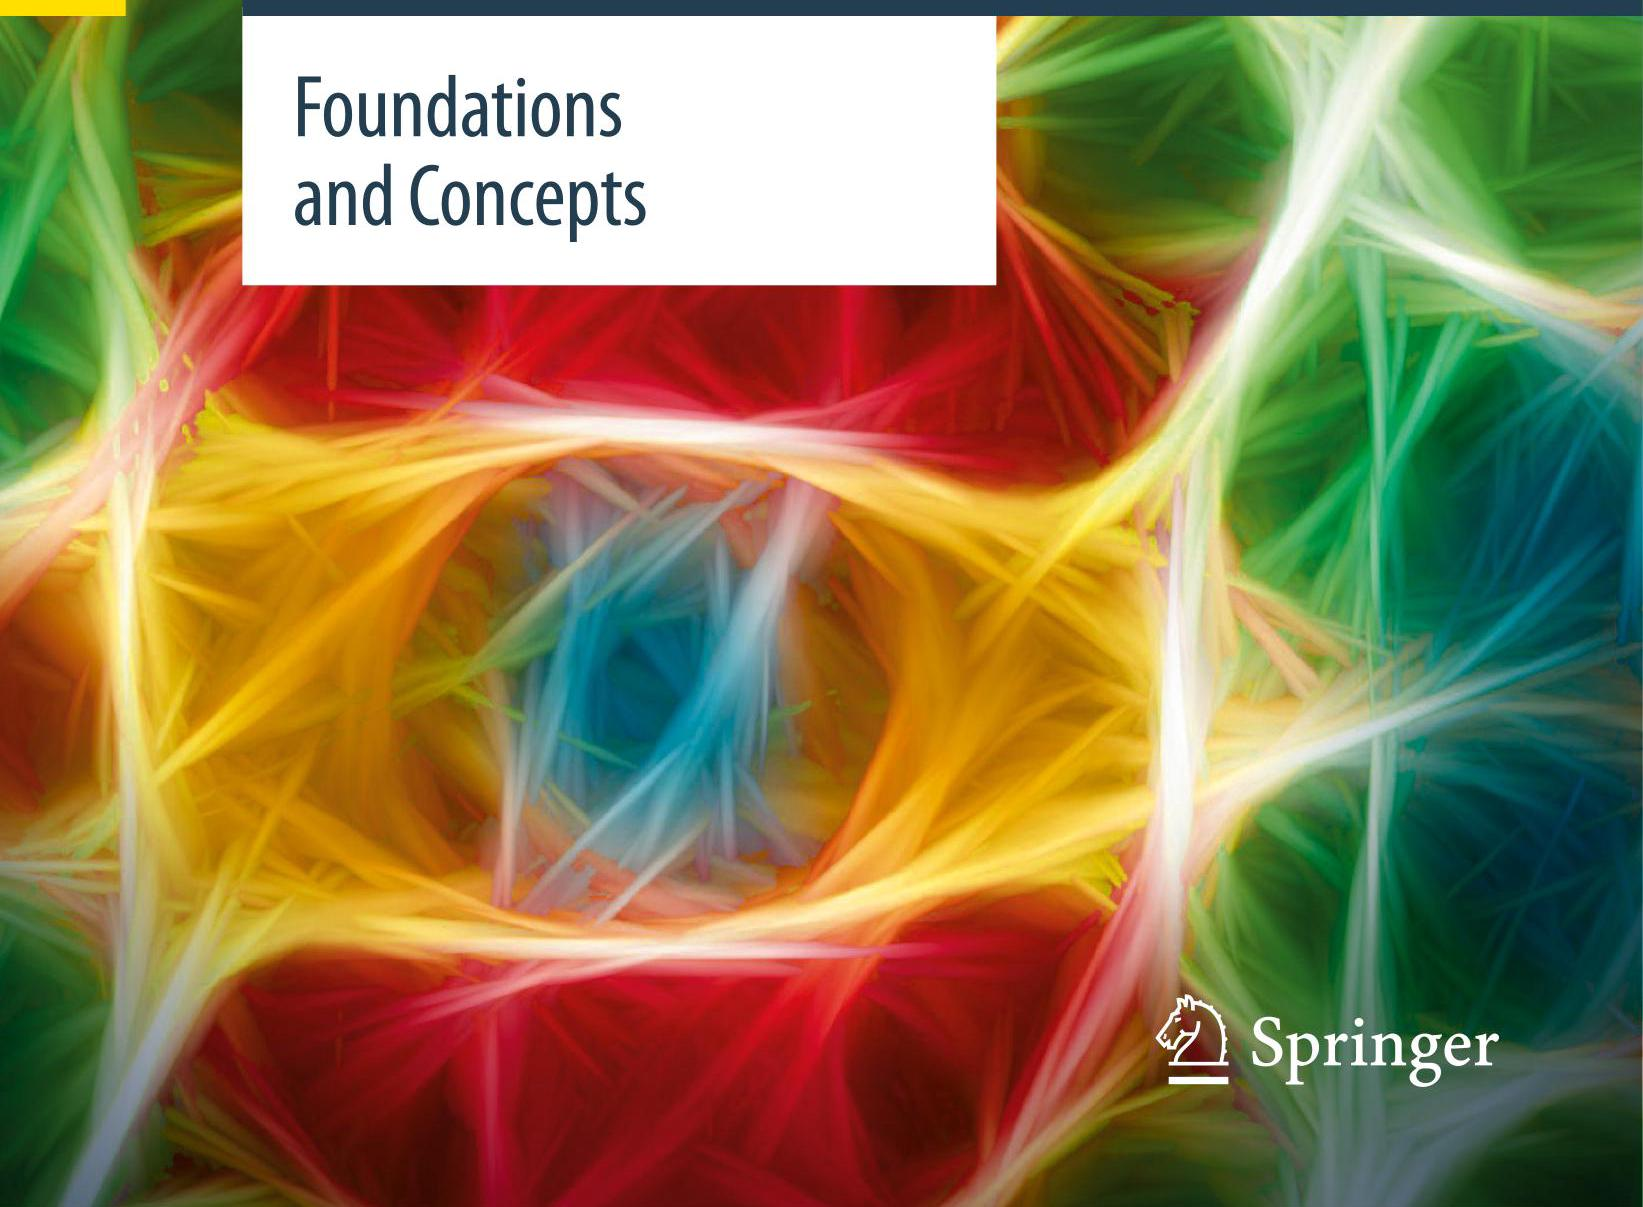
\includegraphics[max width=1.0\textwidth]{images/0194e279-9b28-703a-88f4-c3ac21e2010d_0_0_1124_1643_1207_0.jpg}
\end{center}
\hspace*{3em} 

\customfootnote{

深度学习

}



施普林格自然出版社

Christopher M. Bishop

微软研究院

英国剑桥

休·毕晓普

Wayve 科技有限公司

英国伦敦

ISBN 978 - 3 - 031 - 45467 - 7 ISBN 978 - 3 - 031 - 45468 - 4(电子书)

https://doi.org/10.1007/978-3-031-45468-4

(c) 编辑(如适用)和作者,版权独家授予施普林格自然瑞士股份公司 2024 年

本作品受版权保护。所有权利均由出版商独家许可,无论涉及材料的全部还是部分,特别是翻译、再版、插图再利用、朗诵、广播、缩微胶片复制或以任何其他物理方式复制,以及传输或信息存储与检索、电子改编、计算机软件,或通过现在已知或今后开发的类似或不同方法的权利。

本出版物中使用通用描述性名称、注册商标、商标、服务标记等,即使没有具体声明,也不意味着这些名称不受相关保护法律法规的约束,因此可以自由通用。

出版商、作者和编辑可以放心地认为,本书中的建议和信息在出版日期时被认为是真实和准确的。出版商、作者或编辑均不对本书所含材料或可能出现的任何错误或遗漏作出明示或暗示的保证。出版商在已出版地图的管辖权主张和机构隶属关系方面保持中立。

封面插图:maksimee / 阿拉米图片库

本施普林格品牌由注册公司施普林格自然瑞士股份公司出版

注册公司地址为:Gewerbestrasse 11, 6330 Cham, 瑞士

\section*{前言}

深度学习使用通过大型数据集训练的多层神经网络来解决复杂的信息处理任务,已成为机器学习领域最成功的范式。在过去十年中,深度学习彻底改变了许多领域,包括计算机视觉、语音识别和自然语言处理,并且它正被越来越多地应用于医疗保健、制造业、商业、金融、科学发现等众多领域。最近,被称为大语言模型的大规模神经网络,包含数万亿个可学习参数,已被发现展现出通用人工智能的初步迹象,目前正推动着科技史上最大的变革之一。

\section*{本书目标}

这种不断扩大的影响伴随着机器学习研究出版物数量和范围的激增,创新步伐也在持续加快。对于该领域的新手来说,掌握关键思想,更不用说赶上研究前沿,似乎是一项艰巨的挑战。在此背景下,《深度学习:基础与概念》旨在让机器学习的新手以及该领域的有经验者全面理解支撑深度学习的基础思想,以及现代深度学习架构和技术的关键概念。这些内容将为读者未来的专业学习奠定坚实的基础。由于该领域变化的广度和速度,我们有意避免对最新研究进行全面综述。相反,本书的大部分价值在于对关键思想的提炼,尽管该领域预计将继续快速发展,但这些基础和概念可能会经受住时间的考验。例如,在撰写本书时,大语言模型发展迅速,但底层的变压器(transformer)架构和注意力机制在过去五年中基本保持不变,而许多机器学习的核心原则已经为人所知数十年。

\section*{技术的负责任使用}

深度学习是一项具有广泛适用性的强大技术,它有可能为世界创造巨大价值,并解决一些社会最紧迫的挑战。然而,正是这些特性意味着深度学习也有可能被蓄意滥用,并造成意想不到的危害。我们选择不讨论深度学习应用的伦理或社会层面问题,因为这些主题非常重要且复杂,需要比在这样一本技术教科书中更深入的探讨。不过,这些考量应该建立在对底层技术及其工作原理的扎实理解之上,因此我们希望这本书能为这些重要讨论做出有价值的贡献。尽管如此,我们还是强烈鼓励读者关注其工作的更广泛影响,并在学习技术本身的同时了解深度学习和人工智能的负责任使用。

\section*{本书结构}

本书由数量较多的小章节组成,每一章探讨一个特定主题。本书具有线性结构,即每一章仅依赖于前面章节所涵盖的内容。它非常适合用于教授为期两个学期的本科或研究生机器学习课程,但对于从事积极研究或自学的人同样适用。

只有通过运用一定程度的数学知识,才能清晰理解机器学习。具体而言,机器学习的核心涉及三个数学领域:概率论、线性代数和多元微积分。本书对概率论中所需的概念进行了独立介绍,并包含一个附录总结了线性代数中的一些有用结果。假设读者已经对多元微积分的基本概念有一定了解,不过书中也有附录介绍变分法和拉格朗日乘数法。然而,本书的重点是传达对思想的清晰理解,强调具有现实实用价值的技术,而非抽象理论。在可能的情况下,我们尝试从多个互补的角度呈现更复杂的概念,包括文字描述、图表和数学公式。此外,文中讨论的许多关键算法都在单独的方框中进行了总结。这些总结不涉及计算效率问题,而是作为文中数学解释的补充。因此,我们希望本书的内容能让不同背景的读者都能理解。

从概念上讲,本书或许最自然地被视为《用于模式识别的神经网络》(Bishop,1995b)的后续之作,该书首次从统计角度对神经网络进行了全面探讨。它也可以被视为《模式识别与机器学习》(Bishop,2006)的配套书籍,后者涵盖了机器学习中更广泛的主题,尽管它早于深度学习革命。然而,为确保这本新书内容完整,已从 Bishop(2006)中选取了合适的材料并进行重构,以聚焦于深度学习所需的那些基础思想。这意味着 Bishop(2006)中讨论的许多机器学习有趣主题虽然如今仍然有意义,但已从这本新书中省略。例如,Bishop(2006)深入讨论了贝叶斯方法,而本书几乎完全不涉及贝叶斯方法。

本书配有一个网站,提供支持材料,包括本书的免费数字版、练习答案以及可下载的 PDF 和 JPEG 格式的图表:

\HRule

https://www.bishopbook.com

\HRule

可以使用以下 BibTex 条目引用本书:

\HRule

@book\{Bishop:DeepLearning24,

\hspace*{1em} author = \{Christopher M. Bishop and Hugh Bishop\},

\hspace*{1em} title = \{Deep Learning: Foundations and Concepts\},

\hspace*{1em} year = \{2024\},

\hspace*{1em} publisher = \{Springer\}

\}

\HRule

如果您对本书有任何反馈或想报告任何错误,请将这些内容发送至 feedback@bishopbook.com

\section*{参考文献}

本着专注于核心思想的精神,我们并未尝试提供全面的文献综述,鉴于该领域的规模和变化速度,无论如何这都是不可能的。然而,我们提供了一些关键研究论文、综述文章和其他进一步阅读资料的参考文献。在许多情况下,这些资料还提供了重要的实现细节,为了不使读者分心于正在讨论的核心概念,我们在正文中对这些细节进行了简略处理。

关于机器学习这一主题,尤其是深度学习,已经有很多书籍出版。与本书在水平和风格上最为接近的包括 Bishop (2006)、Goodfellow、Bengio 和 Courville (2016)、Murphy (2022)、Murphy (2023) 以及 Prince (2023)。

在过去十年中,机器学习学术研究的性质发生了显著变化,许多论文在提交给同行评审的会议和期刊之前,甚至取代了这种提交方式,直接发布在在线存档网站上。其中最受欢迎的网站是 arXiv,发音为 “archive”,可在

\HRule

\[
\text{ https://arXiv.org }
\]

\HRule

该网站允许论文进行更新,这通常会导致同一篇论文有与不同年份相关的多个版本,这可能会在引用哪一版本以及对应哪一年的问题上产生一些歧义。它还提供每篇论文的 PDF 免费下载。因此,我们采用了一种简单的方法,即根据首次上传年份来引用论文,不过我们建议阅读最新版本。arXiv 上的论文采用符号 arXiv:YYMM.XXXXX 进行索引,其中 YY 和 MM 分别表示首次上传的年份和月份。后续版本通过在后面添加版本号 \(\mathrm{N}\) 来表示,形式为 arXiv:YYMM.XXXXVN。

\section*{练习}

每章结尾都配有一组练习,旨在强化文中解释的关键概念,或以重要方式对其进行拓展和推广。这些练习是文本的重要组成部分,每个练习都根据难度进行分级,从 \(\left( \star \right)\) (表示只需几分钟就能完成的简单练习)到 \(\left( {\star  \star   \star  }\right)\) (表示复杂得多的练习)。强烈建议读者尝试完成这些练习,因为积极参与学习材料能大大提高学习效果。所有练习的详细解答可从本书的网站以可下载的 PDF 文件形式获取。

\section*{数学符号}

我们采用与 Bishop(2006)相同的符号表示法。关于机器学习背景下的数学概述,请参阅 Deisenroth、Faisal 和 Ong(2020)的著作。

向量用小写粗体罗马字母表示,如 \(\mathbf{x}\) ,而矩阵用大写粗体罗马字母表示,如 M。除非另有说明,所有向量都假定为列向量。上标 T 表示矩阵或向量的转置,因此 \({\mathbf{x}}^{\mathrm{T}}\) 将是一个行向量。符号 \(\left( {{w}_{1},\ldots ,{w}_{M}}\right)\) 表示一个包含 \(M\) 个元素的行向量,对应的列向量写作 \(\mathbf{w} = {\left( {w}_{1},\ldots ,{w}_{M}\right) }^{\mathrm{T}}\) 。 \(M \times  M\) 单位矩阵(也称为幺矩阵)用 \({\mathbf{I}}_{M}\) 表示,如果其维度没有歧义,可缩写为 \(\mathbf{I}\) 。其元素 \({I}_{ij}\) 在 \(i = j\) 时等于 1,在 \(i \neq  j\) 时等于 0。单位矩阵的元素有时用 \({\delta }_{ij}\) 表示。符号 1 表示一个所有元素都为 1 的列向量。 \(\mathbf{a} \oplus  \mathbf{b}\) 表示向量 \(\mathbf{a}\) 和 \(\mathbf{b}\) 的拼接,因此如果 \(\mathbf{a} = \left( {{a}_{1},\ldots ,{a}_{N}}\right)\) 且 \(\mathbf{b} = \left( {{b}_{1},\ldots ,{b}_{M}}\right)\) ,则 \(\mathbf{a} \oplus  \mathbf{b} =\)  \(\left( {{a}_{1},\ldots ,{a}_{N},{b}_{1},\ldots ,{b}_{M}}\right) .\left| x\right|\) 表示标量 \(x\) 的模(正值部分),也称为绝对值。我们用 det \(\mathbf{A}\) 表示矩阵 A 的行列式。

符号 \(x \sim  p\left( x\right)\) 表示 \(x\) 是从分布 \(p\left( x\right)\) 中抽样得到的。当存在歧义时,我们将使用下标,如 \({p}_{x}\left( \cdot \right)\) 来表示所指的是哪个密度。函数 \(f\left( {x,y}\right)\) 关于随机变量 \(x\) 的期望用 \({\mathbb{E}}_{x}\left\lbrack  {f\left( {x,y}\right) }\right\rbrack\) 表示。在对哪个变量进行平均没有歧义的情况下,这将通过省略后缀来简化,例如 \(\mathbb{E}\left\lbrack  x\right\rbrack\) 。如果 \(x\) 的分布以另一个变量 \(z\) 为条件,那么相应的条件期望将写成 \({\mathbb{E}}_{x}\left\lbrack  {f\left( x\right)  \mid  z}\right\rbrack\) 。类似地, \(f\left( x\right)\) 的方差用 \(\operatorname{var}\left\lbrack  {f\left( x\right) }\right\rbrack\) 表示,对于向量变量,协方差写成 \(\operatorname{cov}\left\lbrack  {\mathbf{x},\mathbf{y}}\right\rbrack\) 。我们还将使用 \(\operatorname{cov}\left\lbrack  \mathbf{x}\right\rbrack\) 作为 \(\operatorname{cov}\left\lbrack  {\mathbf{x},\mathbf{x}}\right\rbrack\) 的简写符号。

符号 \(\forall\) 表示 “对于所有”,因此 \(\forall m \in  \mathcal{M}\) 表示集合 \(\mathcal{M}\) 内 \(m\) 的所有值。我们使用 \(\mathbb{R}\) 来表示实数。在图中,节点 \(i\) 的邻居集合用 \(\mathcal{N}\left( i\right)\) 表示,不应将其与高斯分布或正态分布 \(\mathcal{N}\left( {x \mid  \mu ,{\sigma }^{2}}\right)\) 混淆。泛函用 \(f\left\lbrack  y\right\rbrack\) 表示,其中 \(y\left( x\right)\) 是某个函数。泛函的概念在附录 B 中讨论。花括号 \{\} 表示一个集合。符号 \(g\left( x\right)  = \mathcal{O}\left( {f\left( x\right) }\right)\) 表示当 \(x \rightarrow  \infty\) 时 \(\left| {f\left( x\right) /g\left( x\right) }\right|\) 是有界的。例如,如果 \(g\left( x\right)  = 3{x}^{2} + 2\) ,那么 \(g\left( x\right)  = \mathcal{O}\left( {x}^{2}\right)\) 。符号 \(\lfloor x\rfloor\) 表示 \(x\) 的 “向下取整”,即小于或等于 \(x\) 的最大整数。

如果我们有 \(N\) 个独立同分布(i.i.d.)的 \(D\) 维向量 \(\mathbf{x} = {\left( {x}_{1},\ldots ,{x}_{D}\right) }^{\mathrm{T}}\) 的值 \({\mathbf{x}}_{1},\ldots ,{\mathbf{x}}_{N}\) ,我们可以将这些观测值组合成一个维度为 \(N \times  D\) 的数据矩阵 \(\mathbf{X}\) ,其中 \(\mathbf{X}\) 的第 \(n\) 行对应行向量 \({\mathbf{x}}_{n}^{\mathrm{T}}\) 。因此, \(\mathbf{X}\) 的第 \(n,i\) 个元素对应第 \(n\) 个观测值 \({\mathbf{x}}_{n}\) 的第 \(i\) 个元素,并记为 \({x}_{ni}\) 。对于一维变量,我们用 \(\mathbf{x}\) 表示这样的矩阵,它是一个列向量,其第 \(n\) 个元素是 \({x}_{n}\) 。请注意, \(\mathbf{x}\) (维度为 \(N\) )使用了不同的字体以区别于 \(\mathbf{x}\) (维度为 \(D\) )。

\section*{致谢}

我们要向许多审阅各章草稿并提供宝贵反馈的人表示诚挚的感谢。特别地,我们要感谢 Samuel Albanie、Cristian Bodnar、John Bronskill、Wessel Bruinsma、Ignas Budvytis、Chi Chen、Yaoyi Chen、Long Chen、Fergal Cotter、Sam Devlin、Alek - sander Durumeric、Sebastian Ehlert、Katarina Elez、Andrew Foong、Hong Ge、Paul Gladkov、Paula Gori Giorgi、John Gossman、Tengda Han、Juyeon Heo、Katja Hofmann、Chin - Wei Huang、Yongchaio Huang、Giulio Isacchini、Matthew Johnson、Pragya Kale、Atharva Kelkar、Leon Klein、Pushmeet Kohli、Bonnie Kruft、Adrian Li、Haiguang Liu、Ziheng Lu、Giulia Luise、Stratis Markou、Sergio Valcarcel Macua、Krzysztof Maziarz、Matěj Mezera、Laurence Midgley、Usman Munir、Félix Musil、Elise van der Pol、Tao Qin、Isaac Reid、David Rosenberger、Lloyd Russell、Maximilian Schebek、Megan Stanley、Karin Strauss、Clark Templeton、Marlon Tobaben、Aldo Sayeg Pasos - Trejo、Richard Turner、Max Welling、Furu Wei、Robert Weston、Chris Williams、Yingce Xia、Shufang Xie、Iryna Zaporozhets、Claudio Zeni、Xieyuan Zhang 以及许多通过宝贵讨论做出贡献的其他同事。我们还要感谢我们的编辑 Paul Drougas 和施普林格的许多其他人,以及文字编辑 Jonathan Webley,感谢他们在本书制作过程中的支持。

我们要特别感谢 Markus Svensén,他为 Bishop(2006 年)的图表和排版提供了巨大帮助,包括 LTEX 样式文件,这些文件也用于了这本新书。我们也感谢许多允许我们复制他们已发表作品中图表的科学家。具体图表的致谢信息出现在相关的图注中。

Chris 要向微软表示诚挚的感谢,感谢微软创造了一个极富启发性的研究环境,并提供了撰写本书的机会。然而,本书中表达的观点和意见仅代表作者本人,因此不一定与微软或其附属机构的观点相同。能与我的儿子 Hugh 合作编写这本书是一项巨大的荣幸和乐事,这本书最初是在第一次新冠疫情封锁期间作为一个联合项目开始的。X 前言

Hugh 要感谢 Wayve Technologies Ltd 慷慨地允许他兼职工作,使他能够参与本书的撰写,同时也感谢该公司为他提供了一个鼓舞人心且支持性强的工作和学习环境。本书中表达的观点不一定与 Wayve 或其附属机构的观点相同。他要感谢他的未婚妻 Jemima 一直以来的支持,以及她在语法和文体方面的建议。他还要感谢 Chris,Chris 一直是一位优秀的同事,并且在 Hugh 的一生中一直激励着他。

最后,我们俩都想向我们的家人 Jenna 和 Mark 致以最诚挚的感谢,他们为我们做了太多太多的事情,这里实在无法一一列举。仿佛就在很久以前,我们一家人齐聚在安塔利亚的海滩上,观看日全食,并为《模式识别与机器学习》的献词页拍摄了一张全家福!

Chris Bishop 和 Hugh Bishop

英国剑桥

2023 年 10 月


\begin{center}
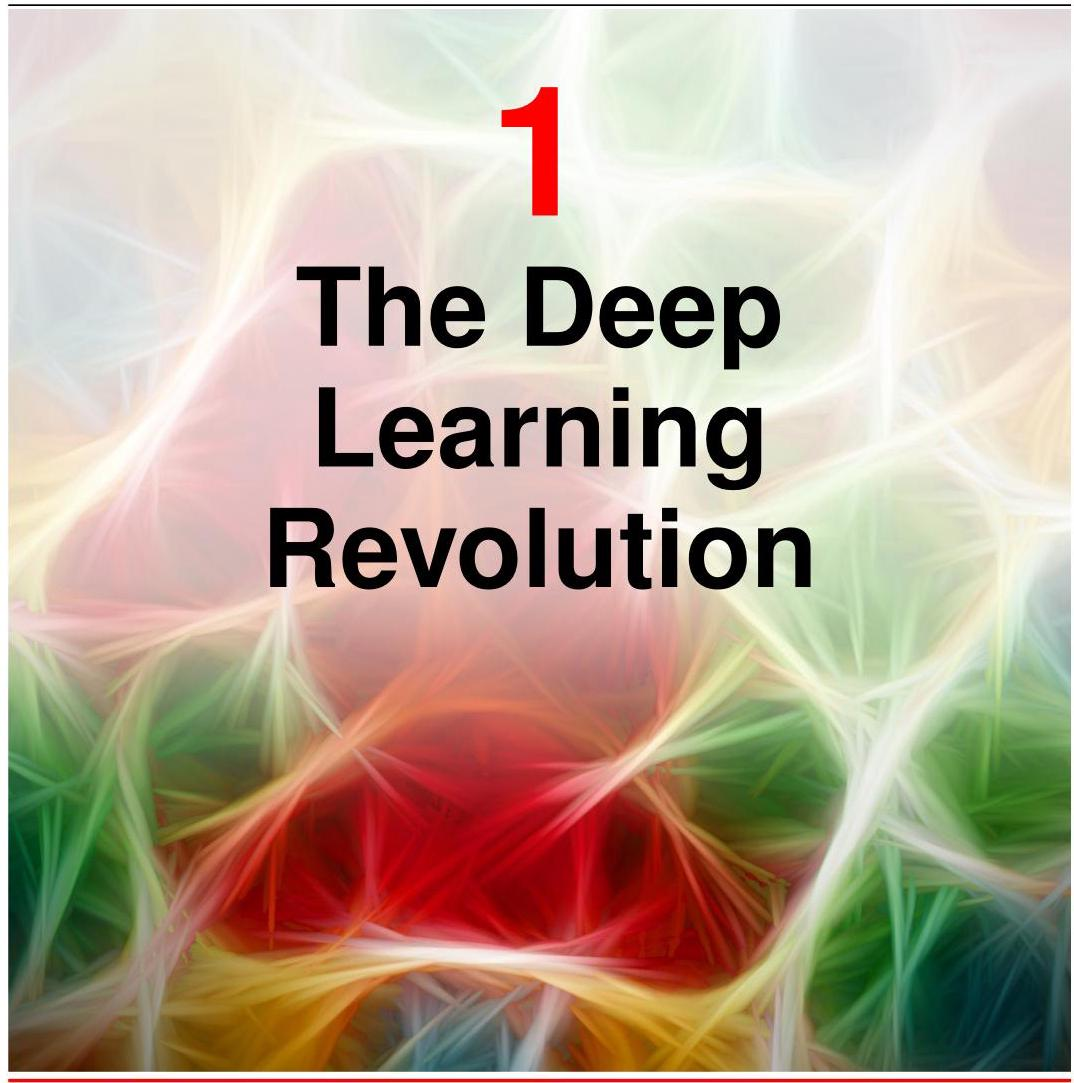
\includegraphics[max width=0.8\textwidth]{images/0194e279-9b28-703a-88f4-c3ac21e2010d_20_474_353_1074_1083_0.jpg}
\end{center}
\hspace*{3em} 

如今,机器学习是最重要且发展最快的技术领域之一。机器学习的应用正变得无处不在,从数据中学习到的解决方案正日益取代传统的手工算法。这不仅提高了现有技术的性能,还为一系列新能力打开了大门,而如果必须手动明确设计新算法,这些能力将是不可想象的。

机器学习的一个特定分支,即深度学习,已成为一种极其强大且通用的数据学习框架。深度学习基于被称为神经网络的计算模型,这些模型最初受到人类大脑学习和信息处理机制的启发。人工智能(AI)领域致力于在机器中重现大脑的强大能力,如今,“机器学习”和“人工智能”这两个术语经常互换使用。当前使用的许多人工智能系统代表了机器学习的应用,这些应用旨在解决非常具体和特定的问题,虽然它们非常有用,但与人类大脑的巨大能力广度相比,仍相去甚远。这导致了“通用人工智能”(AGI)这一术语的引入,用于描述构建具有更大灵活性的机器的愿景。经过数十年的稳步发展,机器学习现在已进入一个快速发展阶段。最近,被称为大语言模型的大规模深度学习系统开始展现出非凡的能力,这些能力被描述为通用人工智能的初步迹象(Bubeck 等人,2023)。

%\chapter{深度深层革命}

\section{深度学习的影响}

我们通过考虑来自不同领域的四个例子来开始对机器学习的讨论,以说明这项技术的广泛适用性,并介绍一些基本概念和术语。这些例子以及许多其他例子特别值得注意的是,它们都使用了深度学习同一基本框架的变体来解决。这与传统方法形成了鲜明对比,在传统方法中,不同的应用使用截然不同的专业技术来处理。应该强调的是,我们选择的例子仅代表了深度神经网络广泛适用性的一小部分,并且几乎每个涉及计算的领域都能受到深度学习的变革性影响。

\subsection{ 医学诊断}

首先考虑机器学习在皮肤癌诊断问题上的应用。黑色素瘤是最危险的皮肤癌类型,但如果早期发现是可以治愈的。图 1.1 展示了皮肤病变的示例图像,上排是恶性黑色素瘤,下排是良性痣。区分这两类图像显然非常具有挑战性,而且几乎不可能手动编写一个算法,能够以合理的准确度成功对这些图像进行分类。

使用深度学习已成功解决了这个问题(Esteva 等人,2017 年)。该解决方案是利用大量的病变图像(即训练集)创建的,其中每张图像都被标记为恶性或良性,这些标签是通过活检测试获得的,该测试被认为能提供病变的真实类别。训练集用于确定深度神经网络中约 2500 万个可调整参数(即权重)的值。这种从数据中设置参数值的过程称为学习或训练。目标是让训练好的网络仅根据新病变的图像就能预测出正确的标签,而无需进行耗时的活检步骤。这是一个监督学习问题的示例,因为对于每个训练样本,网络都被告知正确的标签。这也是一个分类问题的示例,因为每个输入必须被分配到一组离散的类别中(在这种情况下是良性或恶性)。输出由一个或多个连续变量组成的应用称为回归问题。回归问题的一个示例是预测化学制造过程中的产量,其中输入包括温度、压力和反应物浓度。

\begin{center}
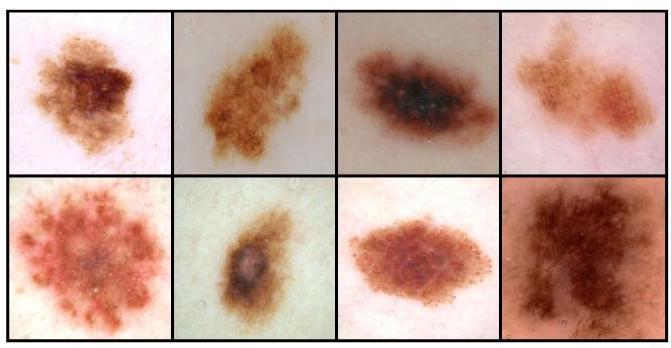
\includegraphics[max width=0.5\textwidth]{images/0194e279-9b28-703a-88f4-c3ac21e2010d_21_871_1649_671_348_0.jpg}
\end{center}
\hspace*{3em} 

图 1.1 上排为危险的恶性黑色素瘤对应的皮肤病变示例,下排为良性痣对应的皮肤病变示例。未经训练的人很难区分这两类病变。

此应用的一个有趣方面是,可用的带标签训练图像数量约为 129,000 张,相对较少,因此深度神经网络首先在一个更大的包含 128 万张日常物品(如狗、建筑物和蘑菇)图像的数据集上进行训练,然后在病变图像数据集上进行微调。这是迁移学习的一个示例,在迁移学习中,网络从日常物品的大数据集中学习自然图像的一般属性,然后专门用于解决病变分类的特定问题。通过使用深度学习,皮肤病变图像的分类准确率已超过专业皮肤科医生(Brinker 等人,2019 年)。

\subsection{蛋白质结构}

蛋白质有时被称为生物体的基石。它们是由一条或多条称为氨基酸的单元长链组成的生物分子,氨基酸有 22 种不同类型,蛋白质由氨基酸序列决定。一旦蛋白质在活细胞内合成,它就会折叠成复杂的三维结构,其行为和相互作用在很大程度上由其形状决定。在已知氨基酸序列的情况下计算这种三维结构,半个世纪以来一直是生物学中一个基本的开放性问题,直到深度学习出现之前进展相对较小。

可以使用 X 射线晶体学、低温电子显微镜或核磁共振光谱等技术通过实验测量三维结构。然而,这可能极其耗时,而且对于某些蛋白质来说可能具有挑战性,例如由于难以获得纯样本或因为结构依赖于环境。相比之下,可以通过实验以较低的成本和较高的通量确定蛋白质的氨基酸序列。因此,人们对能够直接从蛋白质的氨基酸序列预测其三维结构非常感兴趣,以便更好地理解生物过程或用于药物发现等实际应用。可以训练一个深度学习模型,将氨基酸序列作为输入,生成三维结构作为输出,其中训练数据由一组已知氨基酸序列和三维结构的蛋白质组成。因此,蛋白质结构预测是监督学习的另一个示例。一旦系统训练完成,它可以将新的氨基酸序列作为输入,并预测相关的三维结构(Jumper 等人,2021 年)。图 1.2 比较了蛋白质的预测三维结构和通过 \(\mathrm{X}\) 射线晶体学获得的真实结构。

\begin{center}
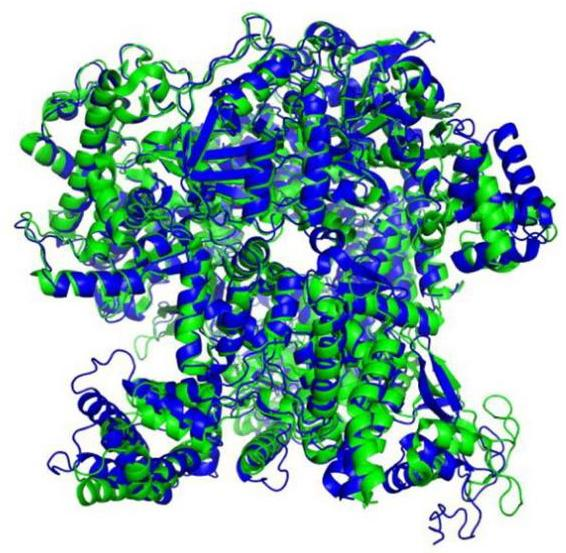
\includegraphics[max width=0.4\textwidth]{images/0194e279-9b28-703a-88f4-c3ac21e2010d_23_983_356_566_553_0.jpg}
\end{center}
\hspace*{3em} 

图 1.2 名为 T1044/6VR4 的蛋白质三维形状示意图。绿色结构显示了通过 X 射线晶体学确定的真实结构,而叠加的蓝色结构显示了由名为 AlphaFold 的深度学习模型获得的预测结果。[经许可摘自 Jumper 等人(2021 年)的研究。]

\subsection{图像合成}

在目前讨论的两个应用中,神经网络学会了将输入(皮肤图像或氨基酸序列)转换为输出(分别为病变分类或蛋白质三维结构)。现在我们来看一个例子,其中训练数据仅由一组样本图像组成,训练好的网络的目标是创建同类的新图像。这是无监督学习的一个例子,因为与病变分类和蛋白质结构的例子不同,这些图像没有标签。图 1.3 展示了由一个在一组在摄影棚纯色背景下拍摄的人脸图像上训练的深度神经网络生成的合成图像示例。这样的合成图像质量极高,很难将它们与真人照片区分开来。

这是生成模型的一个例子,因为它可以生成与用于训练模型的示例不同但具有相同统计特性的新输出示例。这种方法的一个变体允许根据作为提示的输入文本字符串生成图像,从而使图像内容反映文本输入的语义。术语生成式 \({AI}\) 用于描述以图像、视频、音频、文本、候选药物分子或其他形式生成输出的深度学习模型。


\begin{center}
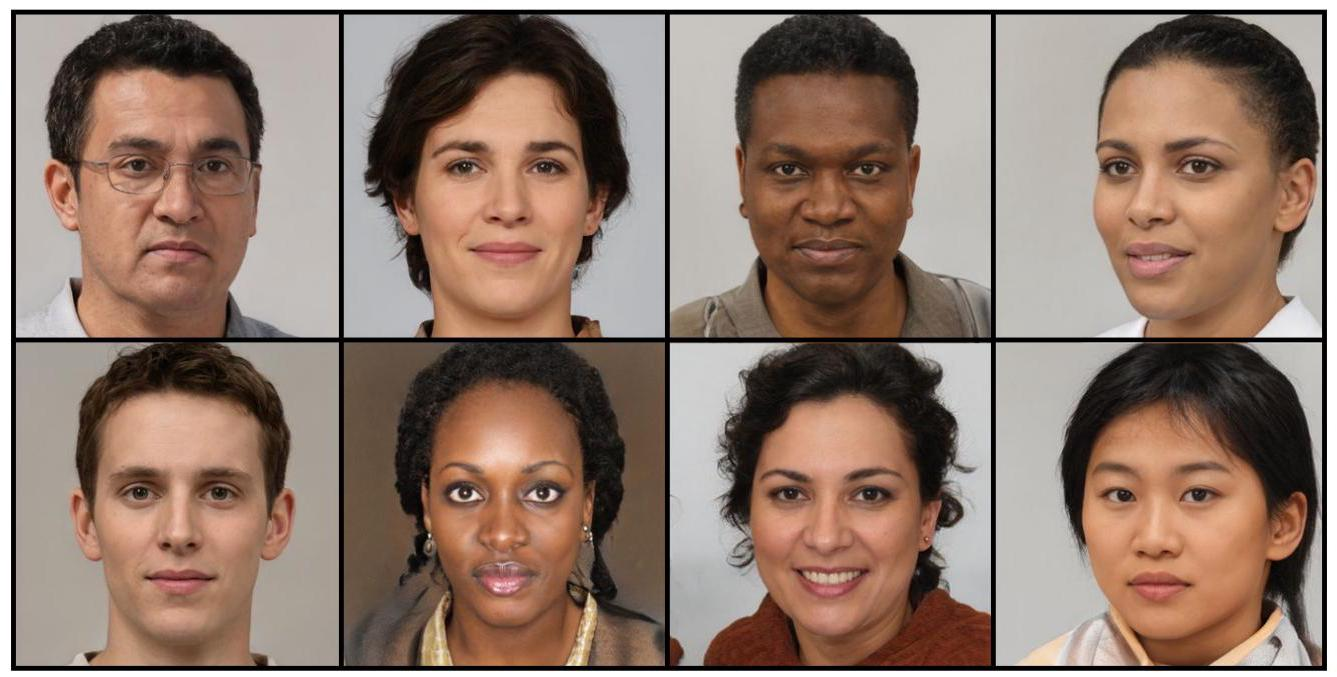
\includegraphics[max width=1.0\textwidth]{images/0194e279-9b28-703a-88f4-c3ac21e2010d_24_231_352_1337_677_0.jpg}
\end{center}
\hspace*{3em} 

图 1.3 通过无监督学习训练的深度神经网络生成的合成人脸图像。[来源:https://generated.photos。]

\subsection{大语言模型}

近年来,机器学习领域最重要的进展之一是开发出了用于处理自然语言和其他形式的序列数据(如源代码)的强大模型。大语言模型(LLM)利用深度学习构建丰富的内部表征,以捕捉语言的语义属性。一类重要的大语言模型,即自回归语言模型,能够生成语言作为输出,因此它们属于生成式人工智能的一种形式。这类模型将一个单词序列作为输入,并输出一个代表该序列中下一个单词的单个单词。将新单词添加到序列末尾形成的增强序列,随后可以再次输入模型以生成后续单词,这个过程可以重复进行,以生成一长串单词。这类模型还可以输出一个特殊的“停止”单词,用于表示文本生成结束,从而使它们能够输出有限长度的文本并停止。此时,用户可以在序列中添加自己的一系列单词,然后将完整的序列再次输入模型,以触发进一步的单词生成。通过这种方式,人类就有可能与神经网络进行对话。

可以在大型文本数据集上对这类模型进行训练,方法是提取训练对,每个训练对由一个随机选择的单词序列作为输入,以及已知的下一个单词作为目标输出组成。这是自监督学习的一个例子,在自监督学习中,学习的是从输入到输出的函数,但标记的输出是自动从输入训练数据中获得的,无需单独的人工标注。由于可以从多个来源获取大量文本,这种方法允许扩展到非常大的训练集和相关的非常大的神经网络。

\begin{center}
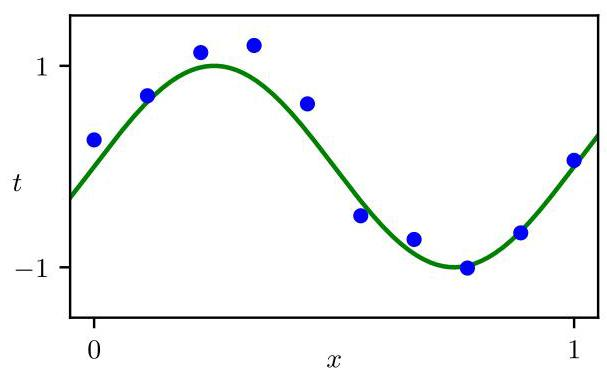
\includegraphics[max width=0.4\textwidth]{images/0194e279-9b28-703a-88f4-c3ac21e2010d_25_946_344_607_378_0.jpg}
\end{center}
\hspace*{3em} 

图 1.4 展示了一个包含 \(N =\) 10 个点的训练数据集,用蓝色圆圈表示,每个点包含输入变量 \(x\) 的一个观测值以及对应的目标变量 \(t\) 。绿色曲线表示用于生成数据的函数 \(\sin \left( {2\pi x}\right)\) 。我们的目标是在不知道绿色曲线的情况下,预测 \(x\) 的某个新值对应的 \(t\) 的值。

大语言模型可以展现出非凡的能力,这些能力被描述为通用人工智能出现的初步迹象(Bubeck 等人,2023),我们将在本书后面详细讨论这类模型。在下一页,我们给出一个语言生成的示例,该示例基于名为 GPT - 4 的模型(OpenAI,2023),响应的输入提示是“写一个证明,证明存在无限多个素数;以莎士比亚戏剧的风格,通过两方就该证明进行争论的对话来完成。”


\subsection{教程示例}

对于机器学习领域的新手来说,许多基本概念和大量术语可以在一个简单示例的背景下引入,该示例涉及将多项式拟合到一个小的合成数据集(Bishop,2006)。这是一种监督学习问题,在这种问题中,我们希望在给定输入变量的值的情况下,对目标变量进行预测。

\subsubsection{合成数据}

我们用 \(x\) 表示输入变量,用 \(t\) 表示目标变量,并且假设这两个变量都在实数轴上取连续值。假设我们得到一个训练集,其中包含 \(N\) 个 \(x\) 的观测值,记为 \({x}_{1},\ldots ,{x}_{N}\) ,以及相应的 \(t\) 的观测值,记为 \({t}_{1},\ldots ,{t}_{N}\) 。我们的目标是对 \(x\) 的某个新值预测 \(t\) 的值。对以前未见过的输入进行准确预测的能力是机器学习的一个关键目标,被称为泛化。

我们可以使用一个从正弦函数采样生成的合成数据集来说明这一点。图 1.4 展示了一个包含 \(N = {10}\) 个数据点的训练集的绘图,其中输入值是通过选择 \({x}_{n}\) 的值生成的,对于 \(n =\)  \(1,\ldots ,N\) ,在范围 \(\left\lbrack  {0,1}\right\rbrack\) 内均匀间隔。相关的目标数据值是通过首先为每个 \(x\) 的值计算函数 \(\sin \left( {2\pi x}\right)\) 的值得到的

\HRule

\section*{GPT-4: Proof of infinitely many primes}

\hspace*{1em} FIRST PARTY:

\hspace*{1em} Thou dost not understand, my friend,

\hspace*{1em} There simply is no upper end

\hspace*{1em} To primes, those numbers indivisible,

\hspace*{1em} No matter if it seems impossible.

\hspace*{1em} SECOND PARTY:

\hspace*{1em} But how dost thou so surely know?

\hspace*{1em} To prove this truth, what canst thou show?

\hspace*{1em} FIRST PARTY:

\hspace*{1em} Consider this, my doubtful peer,

\hspace*{1em} A clever proof that will make clear:

\hspace*{1em} Assume that there's a final prime,

\hspace*{1em} The largest one we'll see in time.

\hspace*{1em} Let's call this number "P" for short,

\hspace*{1em} And then, my friend, we will purport

\hspace*{1em} To build a number " \(Q\) " that's new,

\hspace*{1em} One larger than "P" and prime too.

\hspace*{1em} SECOND PARTY:

\hspace*{1em} But how, my friend, will this be done?

\hspace*{1em} The proof is not yet fairly won.

\hspace*{1em} FIRST PARTY:

\hspace*{1em} It's simple, friend, just wait and see,

\hspace*{1em} We'll multiply the primes, that's key.

\hspace*{1em} All primes from two to " \(\mathrm{P}\) " combined,

\hspace*{1em} Will make this new " \(Q\) " we will find.

\hspace*{1em} But one thing more we must include,

\hspace*{1em} To make the proof more watertight,

\hspace*{1em} We'll add a one onto the end,

\hspace*{1em} And now the proof is in our sight.

\hspace*{1em} SECOND PARTY:

\hspace*{1em} I see it now, it's crystal clear,

\hspace*{1em} For " \(Q\) " must be a prime, my dear.

\hspace*{1em} It can't divide by any prime,

\hspace*{1em} All smaller than itself in time.

\hspace*{1em} And since we chose "P" as the last,

\hspace*{1em} This proves that our assumption's past.

\hspace*{1em} There is no final prime, we see,

\hspace*{1em} The numbers go on endlessly.

\HRule

\HRule

第 2.3 节

\HRule

然后给每个这样的点添加少量的随机噪声(由高斯分布控制),以获得相应的目标值 \({t}_{n}\) 。通过这种方式生成数据,我们捕捉到了许多现实世界数据集的一个重要特性,即它们具有潜在的规律性,我们希望学习这种规律性,但单个观测值会受到随机噪声的干扰。这种噪声可能源于本质上的随机过程(即随机过程),如放射性衰变,但更常见的是由于存在一些本身未被观测到的可变性来源。

在这个教程示例中,我们知道生成数据的真实过程,即正弦函数。在机器学习的实际应用中,我们的目标是在给定有限训练集的情况下发现数据中的潜在趋势。然而,了解生成数据的过程使我们能够阐明机器学习中的重要概念。

\subsubsection{线性模型}

我们的目标是利用这个训练集,为输入变量的某个新值 \(\widehat{x}\) 预测目标变量的值 \(\widehat{t}\) 。正如我们稍后将看到的,这涉及到隐式地尝试发现潜在函数 \(\sin \left( {2\pi x}\right)\) 。这本质上是一个难题,因为我们必须从有限的数据集推广到整个函数。此外,观测数据受到噪声的干扰,因此对于给定的 \(\widehat{x}\) , \(\widehat{t}\) 的合适值存在不确定性。概率论提供了一个框架,用于以精确和定量的方式表达这种不确定性,而决策理论允许我们利用这种概率表示,根据适当的标准做出最优预测。从数据中学习概率是机器学习的核心,本书将对此进行详细探讨。


然而,首先我们将采用较为非正式的方式,考虑一种基于曲线拟合的简单方法。具体而言,我们将使用以下形式的多项式函数来拟合数据

\[
y\left( {x,\mathbf{w}}\right)  = {w}_{0} + {w}_{1}x + {w}_{2}{x}^{2} + \ldots  + {w}_{M}{x}^{M} = \mathop{\sum }\limits_{{j = 0}}^{M}{w}_{j}{x}^{j} \tag{1.1}
\]

其中 \(M\) 是多项式的阶数, \({x}^{j}\) 表示 \(x\) 的 \(j\) 次幂。多项式系数 \({w}_{0},\ldots ,{w}_{M}\) 用向量 \(\mathbf{w}\) 统一表示。请注意,尽管多项式函数 \(y\left( {x,\mathbf{w}}\right)\) 是 \(x\) 的非线性函数,但它是系数 \(\mathbf{w}\) 的线性函数。像这个多项式这样,关于未知参数是线性的函数具有重要的性质,同时也有显著的局限性,这类函数被称为线性模型。



\subsubsection{误差函数}

系数的值将通过使多项式拟合训练数据来确定。这可以通过最小化一个误差函数来实现,该误差函数用于衡量对于任意给定的 \(\mathbf{w}\) 值,函数 \(y\left( {x,\mathbf{w}}\right)\) 与训练集数据点之间的拟合误差。一种广泛使用的简单误差函数选择是
\begin{figure}[!htb]
\begin{center}
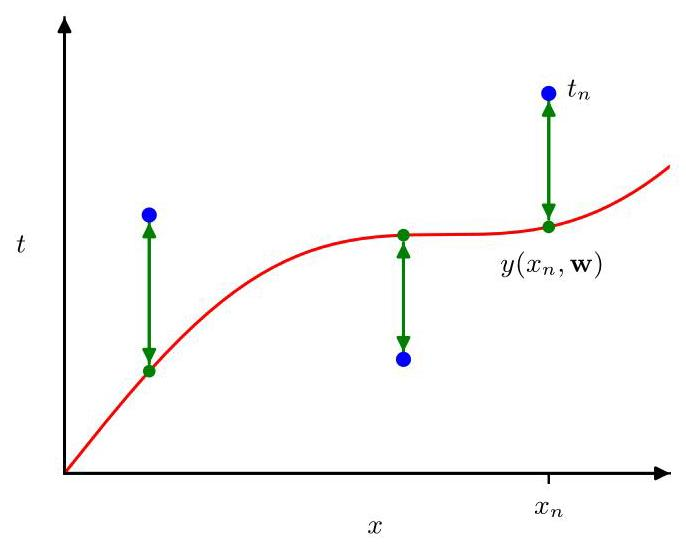
\includegraphics[max width=0.5\textwidth]{images/0194e279-9b28-703a-88f4-c3ac21e2010d_28_873_342_686_544_0.jpg}
\caption{误差函数 (1.2) 对应于每个数据点到函数 \(y\left( {x,\mathbf{w}}\right)\) 的位移(由垂直绿色箭头表示)的平方和的一半。}
\end{center}
\end{figure}
\hspace*{3em} 



每个数据点 \({x}_{n}\) 的预测值 \(y\left( {{x}_{n},\mathbf{w}}\right)\) 与相应目标值 \({t}_{n}\) 之差的平方,由下式给出

\[
E\left( \mathbf{w}\right)  = \frac{1}{2}\mathop{\sum }\limits_{{n = 1}}^{N}{\left\{  y\left( {x}_{n},\mathbf{w}\right)  - {t}_{n}\right\}  }^{2} \tag{1.2}
\]

其中包含因子 \(1/2\) 是为了后续方便。我们稍后将从概率论出发推导这个误差函数。这里我们仅指出,它是一个非负量,当且仅当函数 \(y\left( {x,\mathbf{w}}\right)\) 恰好通过每个训练数据点时,该量才为零。平方和误差函数的几何解释如图 1.5 所示。

\HRule

练习 4.1

\HRule

我们可以通过选择 \(\mathbf{w}\) 的值来解决曲线拟合问题,使得 \(E\left( \mathbf{w}\right)\) 尽可能小。由于误差函数是系数 \(\mathbf{w}\) 的二次函数,它关于系数的导数将是 \(\mathbf{w}\) 元素的线性函数,因此误差函数的最小化有一个唯一解,记为 \({\mathbf{w}}^{ \star  }\) ,可以用封闭形式求出。得到的多项式由函数 \(y\left( {x,{\mathbf{w}}^{ \star  }}\right)\) 给出。



\subsubsection{模型复杂度}

仍然存在选择多项式阶数 \(M\) 的问题,正如我们将看到的,这将是一个被称为模型比较或模型选择的重要概念的示例。在图 1.6 中,我们展示了将阶数为 \(M = 0,1,3\) 和 9 的多项式拟合到图 1.4 所示数据集的四个结果示例。

注意,常数 \(\left( {M = 0}\right)\) 和一阶 \(\left( {M = 1}\right)\) 多项式对数据的拟合效果很差,因此对函数 \(\sin \left( {2\pi x}\right)\) 的表示也很差。三阶 \(\left( {M = 3}\right)\) 多项式似乎在图 1.6 所示的示例中对函数 \(\sin \left( {2\pi x}\right)\) 的拟合效果最好。当我们使用更高阶的多项式 \(\left( {M = 9}\right)\) 时,我们得到了对训练数据的极好拟合。事实上,该多项式恰好通过每个数据点,并且 \(E\left( {\mathbf{w}}^{ \star  }\right)  = 0\) 。然而,拟合曲线剧烈振荡,对函数 \(\sin \left( {2\pi x}\right)\) 的表示非常差。后一种行为被称为过拟合。

\begin{center}
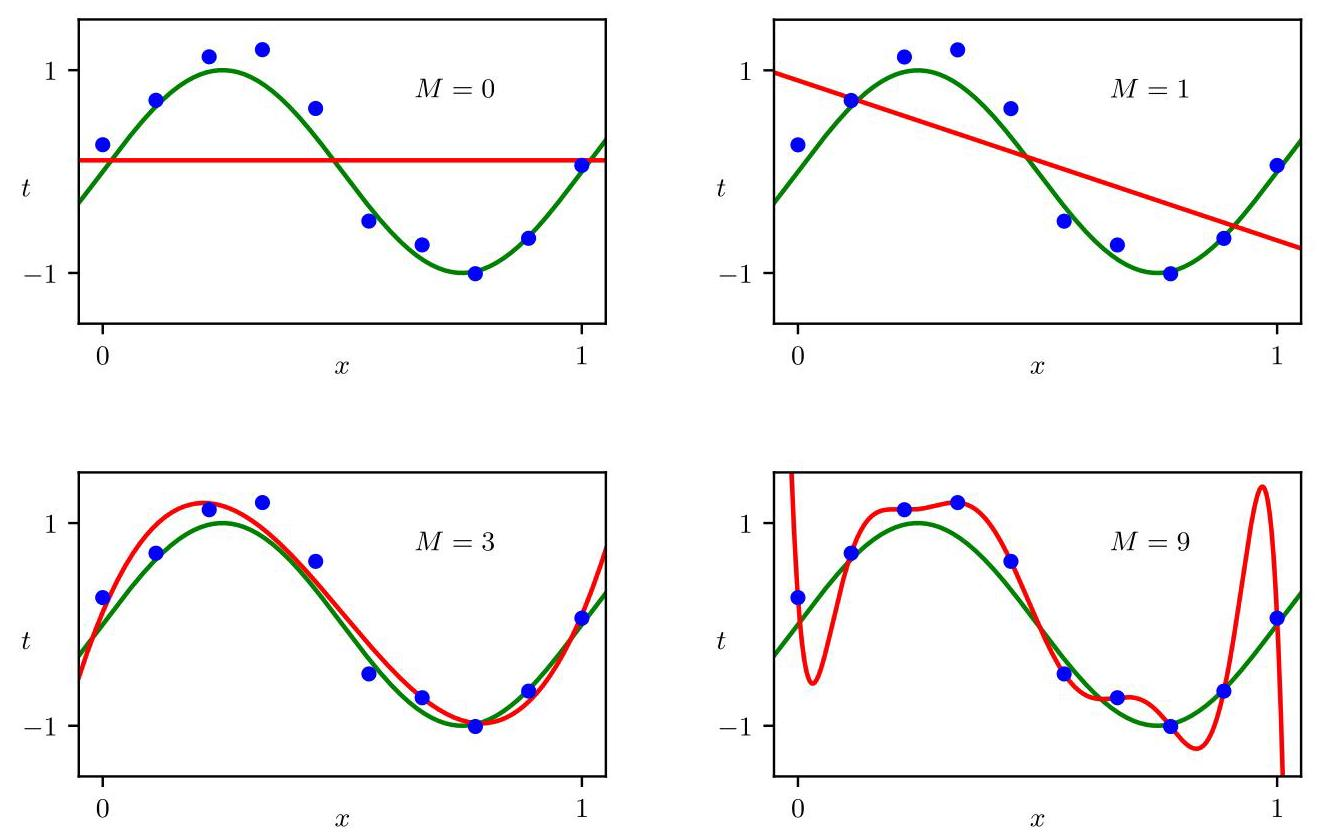
\includegraphics[max width=1.0\textwidth]{images/0194e279-9b28-703a-88f4-c3ac21e2010d_29_237_340_1321_836_0.jpg}
\end{center}
\hspace*{3em} 

图 1.6 展示了通过最小化误差函数 (1.2) 将不同阶数 \(M\) 的多项式(以红色曲线表示)拟合到图 1.4 所示数据集的情况。

我们的目标是通过对新数据进行准确预测来实现良好的泛化。通过考虑一个单独的数据集(称为测试集,包含 100 个使用与生成训练集点相同的过程生成的数据点),我们可以对泛化性能对 \(M\) 的依赖关系获得一些定量的见解。对于 \(M\) 的每个值,我们可以评估由 (1.2) 给出的训练数据的 \(E\left( {\mathbf{w}}^{ \star  }\right)\) 残差值,我们还可以评估测试数据集的 \(E\left( {\mathbf{w}}^{ \star  }\right)\) 。有时,使用由下式定义的均方根 (RMS) 误差来代替评估误差函数 \(E\left( \mathbf{w}\right)\) 会更方便

\[
{E}_{\mathrm{{RMS}}} = \sqrt{\frac{1}{N}\mathop{\sum }\limits_{{n = 1}}^{N}{\left\{  y\left( {x}_{n},\mathbf{w}\right)  - {t}_{n}\right\}  }^{2}} \tag{1.3}
\]

其中除以 \(N\) 使我们能够在同等基础上比较不同大小的数据集,而平方根确保 \({E}_{\mathrm{{RMS}}}\) 与目标变量 \(t\) 在相同的尺度(和相同的单位)上进行测量。训练集和测试集的图表

\begin{center}
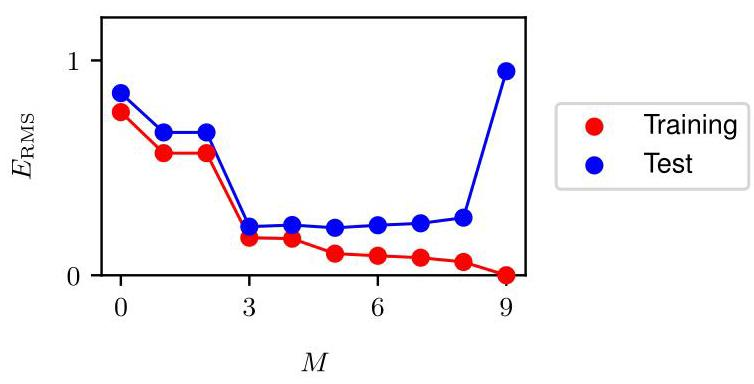
\includegraphics[max width=0.6\textwidth]{images/0194e279-9b28-703a-88f4-c3ac21e2010d_30_794_342_754_384_0.jpg}
\end{center}
\hspace*{3em} 

图 1.7 展示了由 (1.3) 定义的均方根误差在训练集和独立测试集上针对不同 \(M\) 值的评估图表。

均方根误差(RMS errors)针对 \(M\) 的不同取值,如图 1.7 所示。测试集误差衡量了我们对 \(x\) 的新数据观测预测 \(t\) 值的效果。从图 1.7 可以看出, \(M\) 取值较小时,测试集误差相对较大,这可归因于相应的多项式缺乏灵活性,无法捕捉函数 \(\sin \left( {2\pi x}\right)\) 中的振荡。 \(M\) 在 \(3 \leq  M \leq  8\) 范围内取值时,测试集误差较小,并且如图 1.6 中 \(M = 3\) 所示,这些取值也能合理地表示生成函数 \(\sin \left( {2\pi x}\right)\) 。

对于 \(M = 9\) ,训练集误差趋近于零,这正如我们所预期的,因为该多项式包含与 10 个系数 \({w}_{0},\ldots ,{w}_{9}\) 对应的 10 个自由度,因此可以精确地拟合训练集中的 10 个数据点。然而,测试集误差变得非常大,并且如图 1.6 所示,相应的函数 \(y\left( {x,{\mathbf{w}}^{ \star  }}\right)\) 呈现出剧烈的振荡。

这似乎有些矛盾,因为给定阶数的多项式包含所有低阶多项式作为特殊情况。因此, \(M = 9\) 多项式至少能够产生与 \(M = 3\) 多项式一样好的结果。此外,我们可能会认为,对新数据的最佳预测器应该是生成数据的函数 \(\sin \left( {2\pi x}\right)\) (我们稍后会看到情况确实如此)。我们知道函数 \(\sin \left( {2\pi x}\right)\) 的幂级数展开包含所有阶数的项,所以我们可能期望随着 \(M\) 的增加,结果应该单调改善。

通过检查从不同阶数的多项式得到的系数 \({\mathbf{w}}^{ \star  }\) 的值,我们可以对这个问题有更深入的了解,如表 1.1 所示。我们看到,随着 \(M\) 的增加,系数的大小通常会变大。特别是对于 \(M = 9\) 多项式,系数已经针对数据进行了精细调整。它们具有较大的正值和负值,使得相应的多项式函数能够精确匹配每个数据点,但在数据点之间(特别是在范围的两端附近),函数呈现出如图 1.6 中观察到的大幅振荡。直观地说,发生的情况是, \(M\) 值较大的更灵活的多项式越来越适应目标值上的随机噪声。

通过考察随着数据集大小的变化,学习模型的行为,如图 1.8 所示,我们可以对这一现象有更深入的了解。我们看到,对于给定的模型复杂度,随着数据集大小的增加,过拟合问题变得不那么严重。换句话说,有了更大的数据集,我们可以采用更复杂(即更灵活)的模型来拟合数据。经典统计学中有时提倡的一个粗略经验法则是,数据点的数量应该不少于模型中可学习参数数量的某个倍数(例如 5 或 10)。然而,当我们在本书后面讨论深度学习时,我们会看到,使用参数数量明显多于训练数据点数量的模型也能获得出色的结果。

\begin{center}
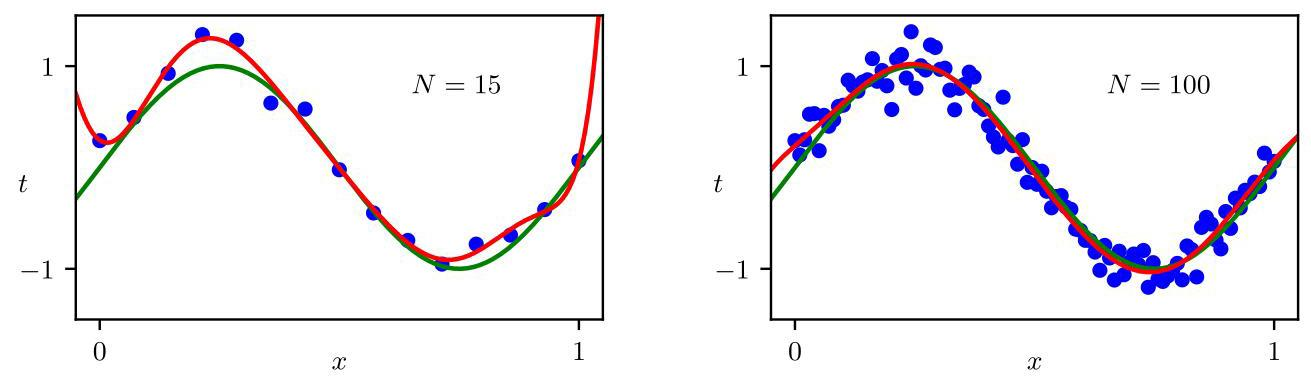
\includegraphics[max width=1.0\textwidth]{images/0194e279-9b28-703a-88f4-c3ac21e2010d_31_240_344_1311_382_0.jpg}
\end{center}
\hspace*{3em} 

图 1.8 展示了使用 \(M = 9\) 多项式,分别对 \(N = {15}\) 个数据点(左图)和 \(N = {100}\) 个数据点(右图)最小化平方和误差函数(1.2)得到的解的绘图。我们看到,增加数据集的大小可以减少过拟合问题。

第 9.3.2 节的数据点。

\section*{1.2.5 正则化}

根据可用训练集的大小来限制模型中参数的数量,这有点不尽如人意。根据待解决问题的复杂度来选择模型的复杂度似乎更为合理。作为限制参数数量的一种替代方法,一种常用于控制过拟合现象的技术是正则化,即在误差函数 (1.2) 中添加一个惩罚项,以防止系数的绝对值过大。最简单的这种惩罚项采用所有系数的平方和的形式,从而得到如下形式的修正误差函数

\[
\widetilde{E}\left( \mathbf{w}\right)  = \frac{1}{2}\mathop{\sum }\limits_{{n = 1}}^{N}{\left\{  y\left( {x}_{n},\mathbf{w}\right)  - {t}_{n}\right\}  }^{2} + \frac{\lambda }{2}\parallel \mathbf{w}{\parallel }^{2} \tag{1.4}
\]

\begin{center}
\adjustbox{max width=\textwidth}{
\begin{tabular}{|c|c|c|c|c|}
\hline
\phantom{X} & \(M = 0\) & \(M = 1\) & \(M = 3\) & \(M = 9\) \\
\cline{1-5}
\({w}_{0}^{ \star  }\) & 0.11 & 0.90 & 0.12 & 0.26 \\
\cline{1-5}
\({w}_{1}^{ \star  }\) & \phantom{X} & -1.58 & 11.20 & -66.13 \\
\cline{1-5}
\({w}_{2}^{ \star  }\) & \phantom{X} & \phantom{X} & -33.67 & 1,665.69 \\
\cline{1-5}
\({w}_{3}^{ \star  }\) & \phantom{X} & \phantom{X} & 22.43 & -15,566.61 \\
\cline{1-5}
\({w}_{4}^{ \star  }\) & \phantom{X} & \phantom{X} & \phantom{X} & 76,321.23 \\
\cline{1-5}
\({w}_{5}^{ \star  }\) & \phantom{X} & \phantom{X} & \phantom{X} & -217,389.15 \\
\cline{1-5}
\({w}_{6}^{ \star  }\) & \phantom{X} & \phantom{X} & \phantom{X} & 370,626.48 \\
\cline{1-5}
\({w}_{7}^{ \star  }\) & \phantom{X} & \phantom{X} & \phantom{X} & -372,051.47 \\
\cline{1-5}
\({w}_{8}^{ \star  }\) & \phantom{X} & \phantom{X} & \phantom{X} & 202,540.70 \\
\cline{1-5}
\({w}_{9}^{ \star  }\) & \phantom{X} & \phantom{X} & \phantom{X} & -46,080.94 \\
\cline{1-5}
\hline
\end{tabular}
}
\end{center}

表 1.1 不同阶多项式的系数 \({w}^{ \star  }\) 表。观察随着多项式阶数的增加,系数的典型大小是如何急剧增加的。

\begin{center}
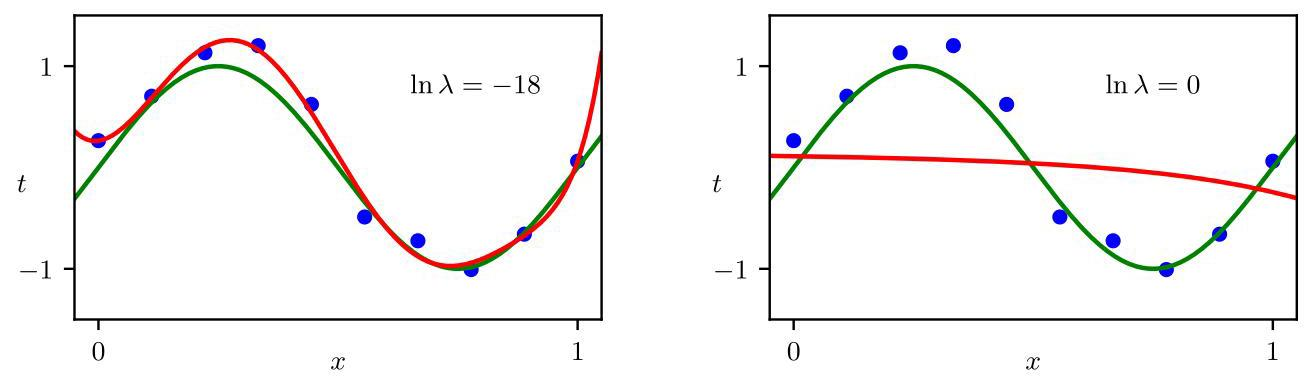
\includegraphics[max width=1.0\textwidth]{images/0194e279-9b28-703a-88f4-c3ac21e2010d_32_240_344_1308_380_0.jpg}
\end{center}
\hspace*{3em} 

图 1.9 展示了使用正则化误差函数 (1.4) 对图 1.4 所示数据集拟合 \(M = 9\) 多项式的结果,正则化参数 \(\lambda\) 取两个值,分别对应 \(\ln \lambda  =  - {18}\) 和 \(\ln \lambda  = 0\) 。无正则化项的情况,即 \(\lambda  = 0\) (对应 \(\ln \lambda  =  - \infty\) ),显示在图 1.6 的右下角。

其中 \(\parallel \mathbf{w}{\parallel }^{2} \equiv  {\mathbf{w}}^{\mathrm{T}}\mathbf{w} = {w}_{0}^{2} + {w}_{1}^{2} + \ldots  + {w}_{M}^{2}\) ,系数 \(\lambda\) 控制着正则化项相对于平方和误差项的相对重要性。请注意,正则化项中通常会省略系数 \({w}_{0}\) ,因为包含它会使结果依赖于目标变量原点的选择(Hastie、Tibshirani 和 Friedman,2009),或者也可以包含它,但要为其设置自己的正则化系数。同样,(1.4) 中的误差函数可以通过封闭形式精确地最小化。在统计学文献中,这类技术被称为收缩方法,因为它们会减小系数的值。在神经网络的背景下,这种方法被称为权重衰减,因为神经网络中的参数被称为权重,而这个正则化项会促使它们向零衰减。

\HRule

第 9.2.1 节

练习 4.2

\HRule

图 1.9 展示了对与之前相同的数据集拟合 \(M = 9\) 阶多项式的结果,但这次使用了 (1.4) 给出的正则化误差函数。我们看到,对于 \(\ln \lambda  =  - {18}\) 的某个值,过拟合现象得到了抑制,现在我们得到了对底层函数 \(\sin \left( {2\pi x}\right)\) 更接近的表示。然而,如果我们为 \(\lambda\) 选择的值过大,那么我们又会得到较差的拟合效果,如图 1.9 中 \(\ln \lambda  = 0\) 的情况所示。拟合多项式得到的相应系数列于表 1.2 中,表明正则化达到了减小系数大小的预期效果。

通过绘制训练集和测试集的均方根误差(1.3)值与 \(\ln \lambda\) 的关系图,可以看出正则化项对泛化误差的影响,如图 1.10 所示。我们发现 \(\lambda\) 现在控制着模型的有效复杂度,从而决定了过拟合的程度。

\begin{center}
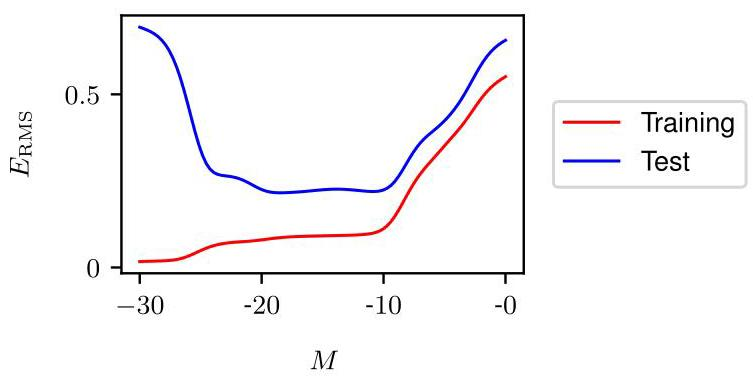
\includegraphics[max width=0.6\textwidth]{images/0194e279-9b28-703a-88f4-c3ac21e2010d_33_798_344_753_382_0.jpg}
\end{center}
\hspace*{3em} 

图 1.10 展示了 \(M = 9\) 多项式的均方根误差(1.3)与 \(\ln \lambda\) 的关系图。

\section*{1.2.6 模型选择}

量 \(\lambda\) 是一个超参数的例子,在最小化误差函数以确定模型参数 \(\mathbf{w}\) 时,其值是固定的。我们不能简单地通过同时相对于 \(\mathbf{w}\) 和 \(\lambda\) 最小化误差函数来确定 \(\lambda\) 的值,因为这将导致 \(\lambda  \rightarrow  0\) 和一个训练误差很小或为零的过拟合模型。类似地,多项式的阶数 \(M\) 是模型的一个超参数,简单地相对于 \(M\) 优化训练集误差将导致 \(M\) 取较大值并产生相关的过拟合。因此,我们需要找到一种方法来确定超参数的合适值。上述结果提出了一种简单的实现方法,即将可用数据划分为训练集(用于确定系数 \(\mathbf{w}\) )和单独的验证集(也称为保留集或开发集)。然后,我们选择在验证集上误差最小的模型。如果使用有限大小的数据集多次迭代进行模型设计,那么可能会对验证数据产生一些过拟合,因此可能需要保留第三个测试集,最终在该测试集上评估所选模型的性能。

对于某些应用,用于训练和测试的数据供应将是有限的。为了构建一个好的模型,我们应该尽可能多地使用可用数据进行训练。然而,如果验证集太小,它将对预测性能给出相对有噪声的估计。解决这个困境的一种方法是使用交叉 -

\begin{center}
\adjustbox{max width=\textwidth}{
\begin{tabular}{|c|c|c|c|}
\hline
\phantom{X} & \(\ln \lambda  =  - \infty\) & \(\ln \lambda  =  - {18}\) & \(\ln \lambda  = 0\) \\
\cline{1-4}
\({w}_{0}^{ \star  }\) & 0.26 & 0.26 & 0.11 \\
\cline{1-4}
\({w}_{1}^{ \star  }\) & -66.13 & 0.64 & -0.07 \\
\cline{1-4}
\({w}_{2}^{ \star  }\) & 1,665.69 & 43.68 & -0.09 \\
\cline{1-4}
\({w}_{3}^{ \star  }\) & -15,566.61 & -144.00 & -0.07 \\
\cline{1-4}
\({w}_{4}^{ \star  }\) & 76,321.23 & 57.90 & -0.05 \\
\cline{1-4}
\({w}_{5}^{ \star  }\) & -217,389.15 & 117.36 & -0.04 \\
\cline{1-4}
\({w}_{6}^{ \star  }\) & 370,626.48 & 9.87 & -0.02 \\
\cline{1-4}
\({w}_{7}^{ \star  }\) & -372,051.47 & -90.02 & -0.01 \\
\cline{1-4}
\({w}_{8}^{ \star  }\) & 202,540.70 & -70.90 & -0.01 \\
\cline{1-4}
\({w}_{9}^{ \star  }\) & -46,080.94 & 75.26 & 0.00 \\
\cline{1-4}
\hline
\end{tabular}
}
\end{center}

表 1.2 正则化参数 \(\lambda\) 取不同值时, \(M = 9\) 多项式的系数 \({w}^{ \star  }\) 表。请注意, \(\ln \lambda  =  - \infty\) 对应于无正则化的模型,即图 1.6 右下角的图。我们看到,随着 \(\lambda\) 值的增加,典型系数的大小会变小。

图 1.11 验证,如图 1.11 所示。这允许将可用数据的一部分 \(\left( {S - 1}\right) /S\) 用于训练,同时利用所有数据来评估性能。当数据特别稀缺时,考虑 \(S = N\) 的情况可能是合适的,其中 \(N\) 是数据点的总数,这就是留一法。

\begin{center}
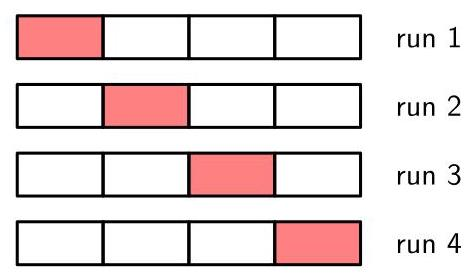
\includegraphics[max width=0.3\textwidth]{images/0194e279-9b28-703a-88f4-c3ac21e2010d_34_1083_343_475_275_0.jpg}
\end{center}
\hspace*{3em} 

1 \(S\) 折交叉验证技术,这里以 \(S = 4\) 的情况为例进行说明,该技术涉及将可用数据划分为 \(S\) 个大小相等的组。然后使用 \(S - 1\) 个组来训练一组模型,然后在剩余的组上对这些模型进行评估。然后对保留组的所有 \(S\) 种可能选择重复此过程,这里用红色块表示,然后对 \(S\) 次运行的性能得分进行平均。

交叉验证的主要缺点是必须执行的训练运行次数增加了 \(S\) 倍,对于训练本身计算成本较高的模型来说,这可能会成为问题。像交叉验证这样使用单独数据来评估性能的技术的另一个问题是,对于单个模型,我们可能有多个复杂度超参数(例如,可能有几个正则化超参数)。在最坏的情况下,探索此类超参数的设置组合可能需要进行的训练运行次数与超参数的数量呈指数关系。现代机器学习的前沿涉及极其庞大的模型,这些模型在相应庞大的数据集上进行训练。因此,探索超参数设置的空间有限,并且在很大程度上依赖于使用较小模型获得的经验和启发式方法。

这个将多项式拟合到由正弦函数生成的合成数据集的简单示例说明了机器学习中的许多关键思想,我们将在后续章节中进一步使用这个示例。然而,机器学习的实际应用在几个重要方面有所不同。用于训练的数据集的大小可能要大几个数量级,并且通常会有更多的输入变量,例如在图像分析中可能有数百万个,以及多个输出变量。将输出与输入相关联的可学习函数由一类称为神经网络的模型控制,这些模型可能有大量的参数,可能多达数千亿个,并且误差函数将是这些参数的高度非线性函数。误差函数不能再通过闭式解来最小化,而是必须通过基于误差函数相对于参数的导数评估的迭代优化技术来最小化,所有这些都可能需要专门的计算硬件并产生大量的计算成本。

\begin{center}
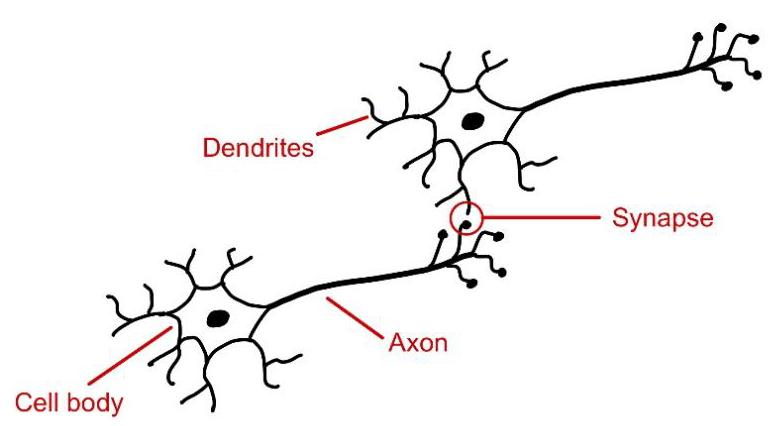
\includegraphics[max width=0.6\textwidth]{images/0194e279-9b28-703a-88f4-c3ac21e2010d_35_755_356_776_426_0.jpg}
\end{center}
\hspace*{3em} 

图 1.12 显示人脑两个神经元的示意图。这些电活性细胞通过称为突触的连接进行通信,随着网络学习,突触的强度会发生变化。

\section*{1.3. 机器学习简史}

机器学习有着悠久而丰富的历史,包括对多种替代方法的探索。在这里,我们专注于基于神经网络的机器学习方法的演变,因为这些方法是深度学习的基础,并且已被证明是现实世界应用中最有效的机器学习方法。

神经网络模型最初受到对人类和其他哺乳动物大脑信息处理研究的启发。大脑中的基本处理单元是具有电活性的细胞,称为神经元,如图 1.12 所示。当一个神经元“放电”时,它会沿着轴突发送电脉冲,到达称为突触的连接点,这些突触与其他神经元形成连接。在突触处会释放称为神经递质的化学信号,这些信号可以刺激或抑制后续神经元的放电。

人类大脑总共包含约 900 亿个神经元,每个神经元平均与其他神经元有数千个突触,形成一个总共约有 100 万亿 \(\left( {10}^{14}\right)\) 个突触的复杂网络。如果某个特定的神经元从其他神经元的放电中接收到足够的刺激,那么它也会被诱导放电。然而,一些突触具有负面或抑制作用,即输入神经元的放电会降低输出神经元放电的可能性。一个神经元促使另一个神经元放电的程度取决于突触的强度,而这些强度的变化代表了大脑存储信息和从经验中学习的关键机制。

神经元的这些特性已被非常简单的数学模型所捕捉,这些模型被称为人工神经网络,它们随后构成了计算学习方法的基础(McCulloch 和 Pitts,1943)。许多这些模型通过形成其他神经元输出的线性组合来描述单个神经元的特性,然后使用非线性函数对其进行变换。这可以用数学形式表示为

\[
a = \mathop{\sum }\limits_{{i = 1}}^{M}{w}_{i}{x}_{i} \tag{1.5}
\]

\[
y = f\left( a\right)  \tag{1.6}
\]

\begin{center}
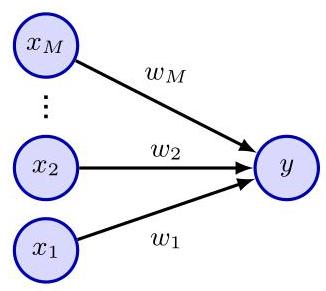
\includegraphics[max width=0.2\textwidth]{images/0194e279-9b28-703a-88f4-c3ac21e2010d_36_1225_345_326_291_0.jpg}
\end{center}
\hspace*{3em} 

图 1.13 一个简单的神经网络图,代表描述单个神经元的变换 (1.5) 和 (1.6)。多项式函数 (1.1) 可以看作是该模型的一个特例。

其中 \({x}_{1},\ldots ,{x}_{M}\) 表示 \(M\) 输入,这些输入对应于向该神经元发送连接的其他神经元的活动,而 \({w}_{1},\ldots ,{w}_{M}\) 是连续变量,称为权重,它们表示相关突触的强度。量 \(a\) 称为预激活,非线性函数 \(f\left( \cdot \right)\) 称为激活函数,输出 \(y\) 称为激活。我们可以看到,多项式 (1.1) 可以看作是这种表示的一个特定实例,其中输入 \({x}_{i}\) 由单个变量 \(x\) 的幂给出,并且函数 \(f\left( \cdot \right)\) 只是恒等函数 \(f\left( a\right)  = a\) 。由 (1.5) 和 (1.6) 给出的简单数学公式从 20 世纪 60 年代至今一直是神经网络模型的基础,并且可以用如图 1.13 所示的图表形式表示。

\section*{1.3.1 单层网络}

人工神经网络的历史大致可以根据处理“层”的数量衡量的网络复杂程度分为三个不同的阶段。由 (1.5) 和 (1.6) 描述的简单神经模型可以看作具有单层处理,对应于图 1.13 中的单层连接。神经计算历史上最重要的此类模型之一是感知机(Rosenblatt,1962),其中激活函数 \(f\left( \cdot \right)\) 是形式为

\[
f\left( a\right)  = \left\{  \begin{array}{ll} 0, & \text{ if }a \leq  0 \\  1, & \text{ if }a > 0 \end{array}\right.  \tag{1.7}
\]

这可以看作是神经放电的简化模型,其中一个神经元当且仅当总加权输入超过阈值 0 时才会放电。感知机由 Rosenblatt(1962)开创,他开发了一种特定的训练算法,该算法具有一个有趣的性质:如果存在一组权重值使得感知机能够对其训练数据进行完美分类,那么该算法保证能在有限步骤内找到解决方案(Bishop,2006)。除了学习算法,感知机还有专门的模拟硬件实现,如图 1.14 所示。典型的感知机构型有多层处理,但只有其中一层可以从数据中学习,因此感知机被认为是“单层”神经网络。

\begin{center}
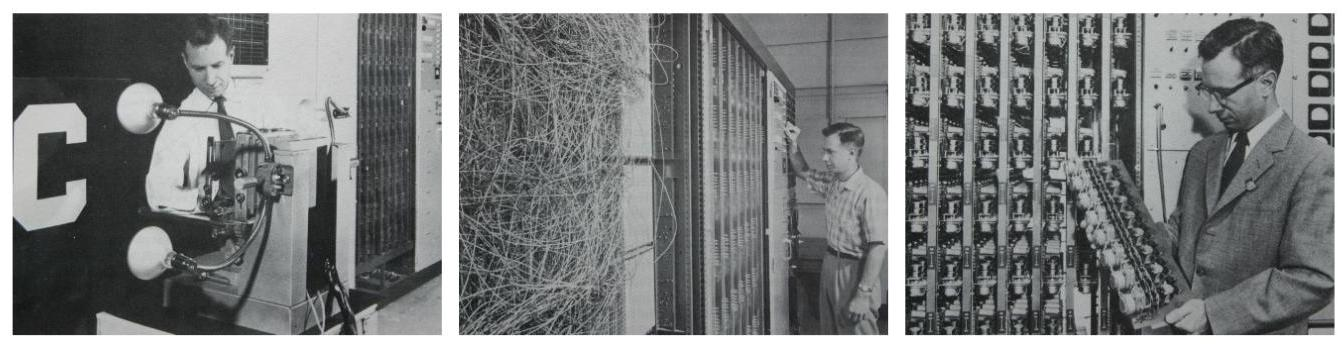
\includegraphics[max width=1.0\textwidth]{images/0194e279-9b28-703a-88f4-c3ac21e2010d_37_207_344_1342_344_0.jpg}
\end{center}
\hspace*{3em} 

图 1.14 Mark 1 感知机硬件示意图。左边的照片展示了如何使用简单的相机系统获取输入,在该系统中,输入场景(在这种情况下是一个印刷字符)被强光照射,图像聚焦到 \({20} \times  {20}\) 硫化镉光电管阵列上,得到一个原始的 400 像素图像。感知机还有一个接线板,如中间照片所示,它允许尝试不同的输入特征配置。通常这些接线是随机连接的,以展示感知机无需精确接线就能学习的能力,这与现代数字计算机形成对比。右边的照片展示了可学习权重的机架之一。每个权重使用旋转可变电阻器(也称为电位计)实现,由电动机驱动,从而允许学习算法自动调整权重值。

起初,感知机以类似大脑的方式从数据中学习的能力被认为非常了不起。然而,很明显该模型也有重大局限性。Minsky 和 Papert(1969)分析了感知机的性质,他们正式证明了单层网络的能力有限。不幸的是,他们还推测类似的局限性也会扩展到具有多层可学习参数的网络。尽管后一个猜想被证明是大错特错的,但这一影响抑制了人们对神经网络模型的热情,这导致了 20 世纪 70 年代和 80 年代初人们对神经网络缺乏兴趣和资金投入。此外,由于缺乏有效的训练算法,研究人员无法探索多层网络的性质,因为诸如感知机算法之类的技术仅适用于单层模型。请注意,尽管感知机早已从实际机器学习中消失,但这个名称仍然存在,因为现代神经网络有时也被称为多层感知机或 MLP。

\section*{1.3.2 反向传播}

训练具有多层可学习参数的神经网络问题的解决方案来自于微积分的运用以及基于梯度的优化方法的应用。一个重要的改变是用具有非零梯度的连续可微激活函数取代阶跃函数(1.7)。另一个关键修改是引入可微误差函数,这些函数定义了给定的参数值选择在多大程度上能够预测训练集中的目标变量。当我们讨论模型的形式或训练方式时,我们看到了这样一个误差函数的例子。

\begin{center}
\adjustbox{max width=\textwidth}{
\begin{tabular}{|c|c|c|}
\hline
图 1.15 & 一个具有两层参数的神经网络,其中箭头表示信息在网络中的流动方向。每个隐藏单元和每个输出单元都计算由 (1.5) 和 (1.6) 给出形式的函数,其中激活函数 \(f\left( \cdot \right)\) 是可微的。 & 隐藏单元 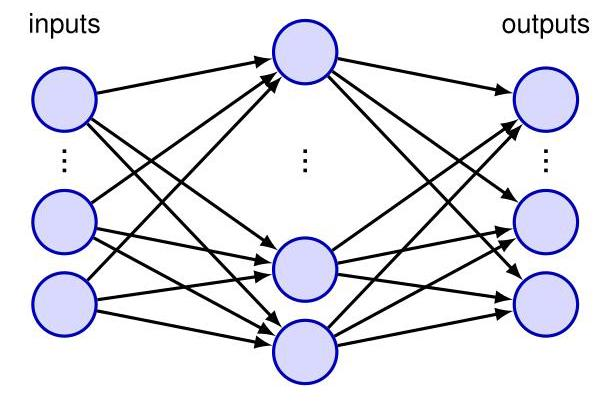
\includegraphics[max width=0.4\textwidth]{images/0194e279-9b28-703a-88f4-c3ac21e2010d_38_944_397_604_402_0.jpg} \\
\cline{1-3}
第 1.2.3 节 & \multicolumn{2}{|c|}{使用平方和误差函数 (1.2) 来拟合多项式。有了这些变化,我们现在有了一个误差函数,其关于网络中每个参数的导数可以被计算。我们现在可以考虑具有多层参数的网络。图 1.15 展示了一个具有两个处理层的简单网络。中间层的节点被称为隐藏单元,因为它们的值不出现在训练集中,训练集仅提供输入和输出的值。图 1.15 中的每个隐藏单元和每个输出单元都计算由 (1.5) 和 (1.6) 给出形式的函数。对于给定的一组输入值,所有隐藏单元和输出单元的状态可以通过重复应用 (1.5) 和 (1.6) 来计算,其中信息沿着箭头方向在网络中向前流动。出于这个原因,这样的模型有时也被称为前馈神经网络。为了训练这样的网络,首先使用随机数生成器初始化参数,然后使用基于梯度的优化技术迭代更新这些参数。这涉及计算误差函数的导数,} \\
\cline{1-3}
第 8 章 第 7 章 & 即随机梯度下降。 & 可以在被称为误差反向传播的过程中高效完成。在反向传播中,信息通过网络从输出端向输入端反向流动(Rumelhart、Hinton 和 Williams,1986 年)。存在许多不同的优化算法,它们利用待优化函数的梯度,但机器学习中最常用的也是最简单的一种,被称为能够训练具有多层权重的神经网络是一项突破,这导致从 20 世纪 80 年代中期左右开始,该领域的研究兴趣再度兴起。这也是该领域超越对神经生物学启发的关注,并发展出更严谨、更有原则的基础的时期(Bishop,1995b)。特别是,人们认识到概率论以及统计学领域的思想在神经网络和机器学习中起着核心作用。一个关键的见解是,从数据中学习涉及背景假设,有时被称为先验知识或归纳偏差。这些假设可以被明确纳入,例如通过设计神经网络的结构,使得皮肤病变的分类不依赖于病变在图像中的位置,或者它们可能以从数学中产生的隐含假设的形式存在 \\
\cline{1-3}
\hline
\end{tabular}
}
\end{center}

反向传播和基于梯度的优化方法的发展极大地提升了神经网络解决实际问题的能力。然而,人们也注意到,在多层网络中,只有最后两层的权重能够学习到有用的值。除了少数例外,特别是被称为卷积神经网络的用于图像分析的模型(LeCun 等人,1998),层数超过两层的网络成功应用案例非常少。这再次限制了这些类型网络能够有效解决的问题的复杂性。为了在许多应用中取得合理的性能,有必要使用手工设计的预处理方法将输入变量转换到一个新的空间,期望在这个空间中机器学习问题更容易解决。这个预处理阶段有时也被称为特征提取。尽管这种方法有时是有效的,但如果能够从数据中学习特征而不是手工设计,显然会更好。

\HRule

第 10 章

\HRule

到新千年开始时,现有的神经网络方法再次达到了其能力的极限。研究人员开始探索一系列神经网络的替代方法,如核方法、支持向量机、高斯过程等等。神经网络再次失宠,尽管一群热情的研究人员继续追求一种真正有效的方法来训练多层网络的目标。

\section*{1.3.3 深度网络}

神经网络发展的第三个也是当前的阶段始于 21 世纪的第二个十年。一系列的发展使得具有多层权重的神经网络能够被有效训练,从而消除了这些技术先前的能力限制。具有多层权重的网络被称为深度神经网络,专注于此类网络的机器学习子领域被称为深度学习(LeCun、Bengio 和 Hinton,2015)。

深度学习起源中的一个重要主题是神经网络规模(以参数数量衡量)的显著增加。尽管在 20 世纪 80 年代,具有几百或几千个参数的网络很常见,但这个数字稳步上升到数百万,然后是数十亿,而目前最先进的模型可能有大约一万亿(10 \({}^{12}\) )个参数。具有大量参数的网络需要相应的大规模数据集,以便训练信号能够为这些参数产生良好的值。大规模模型和大规模数据集的结合反过来又要求在训练模型时进行大规模计算。被称为图形处理单元(GPU)的专用处理器最初是为视频游戏等应用快速渲染图形数据而开发的,事实证明它非常适合神经网络的训练,因为网络一层中的单元所计算的函数可以并行评估,这与 GPU 的大规模并行性非常匹配(Krizhevsky、Sutskever 和 Hinton,2012)。如今,最大模型的训练是在由数千个通过专用高速互连连接的 GPU 组成的大型阵列上进行的。

\begin{center}
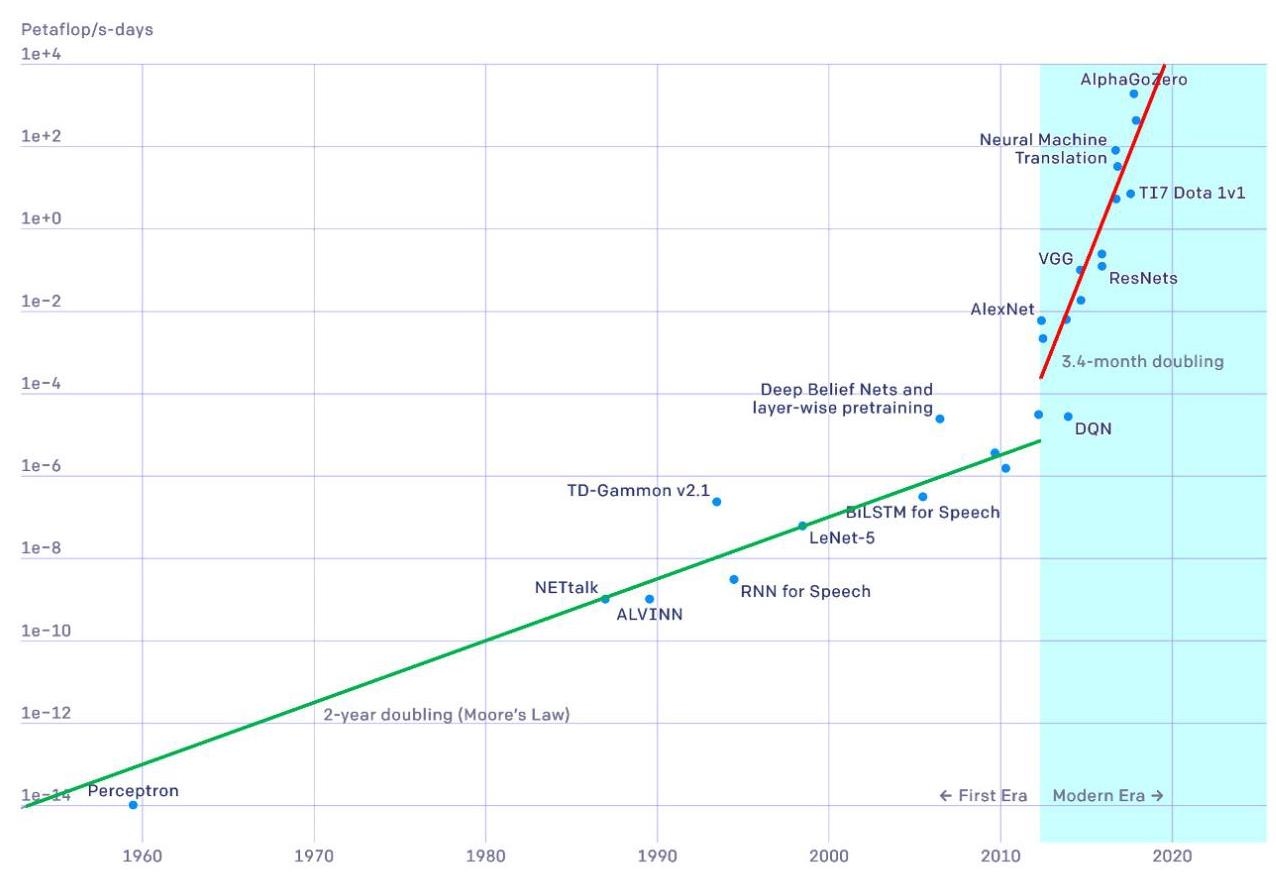
\includegraphics[max width=1.0\textwidth]{images/0194e279-9b28-703a-88f4-c3ac21e2010d_40_255_347_1276_882_0.jpg}
\end{center}
\hspace*{3em} 

图 1.16 绘制了训练最先进的神经网络所需的计算周期数(以千万亿次浮点运算每秒 - 天为单位)随日期的变化情况,显示出两个不同的指数增长阶段。[经 OpenAI 许可使用。]

图 1.16 展示了多年来训练最先进的神经网络所需的计算周期数是如何增长的,呈现出两个不同的增长阶段。纵轴采用指数刻度,单位为千万亿次浮点运算每秒 - 天,其中千万亿次浮点运算表示 \({10}^{15}\) (一千万亿)次浮点运算,而千万亿次浮点运算每秒是指每秒进行一千万亿次浮点运算。一个千万亿次浮点运算每秒 - 天表示以千万亿次浮点运算每秒的速率进行 24 小时的计算,大约是 \({10}^{20}\) 次浮点运算,因此,图中的顶线代表了令人印象深刻的 10 \({}^{24}\) 次浮点运算。图中的直线表示指数增长,我们可以看到,从感知机时代到 2012 年左右,翻倍时间约为 2 年,这与摩尔定律导致的计算能力的总体增长相一致。从 2012 年开始,即深度学习时代,我们再次看到指数增长,但现在的翻倍时间为 3.4 个月,相当于计算能力每年增长 10 倍!

人们常常发现,由于架构创新或引入更复杂的归纳偏置形式而带来的性能提升很快就会......

\begin{center}
\adjustbox{max width=\textwidth}{
\begin{tabular}{|c|c|}
\hline
第12.3.5节提到,这种在语义上有意义的表示方式,为最后一层或多层解决问题创造了更简单的条件。正如我们在皮肤病变分类中所看到的,通过迁移学习,这种内部表示可以被重新利用,以解决相关问题。值得注意的是,用于处理图像的神经网络 & 仅仅通过增加训练数据的数量,以及相应地扩大模型规模和用于训练的计算能力,就可以被超越(Sutton,2019)。大型模型不仅在特定任务上可能表现更优,而且还能够使用同一个经过训练的神经网络解决更广泛的不同问题。大语言模型就是一个显著的例子,因为单个网络不仅具有非凡的能力广度,甚至能够超越专门为解决特定问题而设计的专业网络。我们已经看到,深度在使神经网络实现高性能方面起着重要作用。看待深度神经网络中隐藏层作用的一种方式是将其视为表示学习(Bengio、Courville和Vincent,2012),在这种学习中,网络学习将输入数据转换为一种新的表示 \\
\cline{1-2}
第10.3节 & 可能学习到与哺乳动物视觉皮层中观察到的表示非常相似的内部表示。能够适应或微调以用于一系列下游任务的大型神经网络被称为基础模型,它们可以利用大型、异构数据集来创建具有广泛适用性的模型(Bommasani等人,2021)。除了扩展规模之外,还有其他一些发展有助于深度学习的成功。例如,在简单的神经网络中,训练信号在通过深度网络的连续层进行反向传播时会变弱 \\
\cline{1-2}
第9.5节 & 。解决这个问题的一种技术是引入残差连接(He等人,2015a),它有助于训练具有数百层的网络。另一个关键的发展是引入了自动微分方法,在这种方法中,用于执行反向传播以评估误差函数梯度的代码是从用于指定前向传播的代码自动生成的。这使得研究人员能够快速尝试不同的神经网络架构,并非常容易地以多种方式组合不同的架构元素,因为只需要显式地编写相对简单的前向传播函数。此外,机器学习领域的许多研究都是通过开源进行的,这使得研究人员能够在他人的工作基础上进行研究,从而进一步加快了该领域的进展速度。 \\
\cline{1-2}
\hline
\end{tabular}
}
\end{center}

\begin{center}
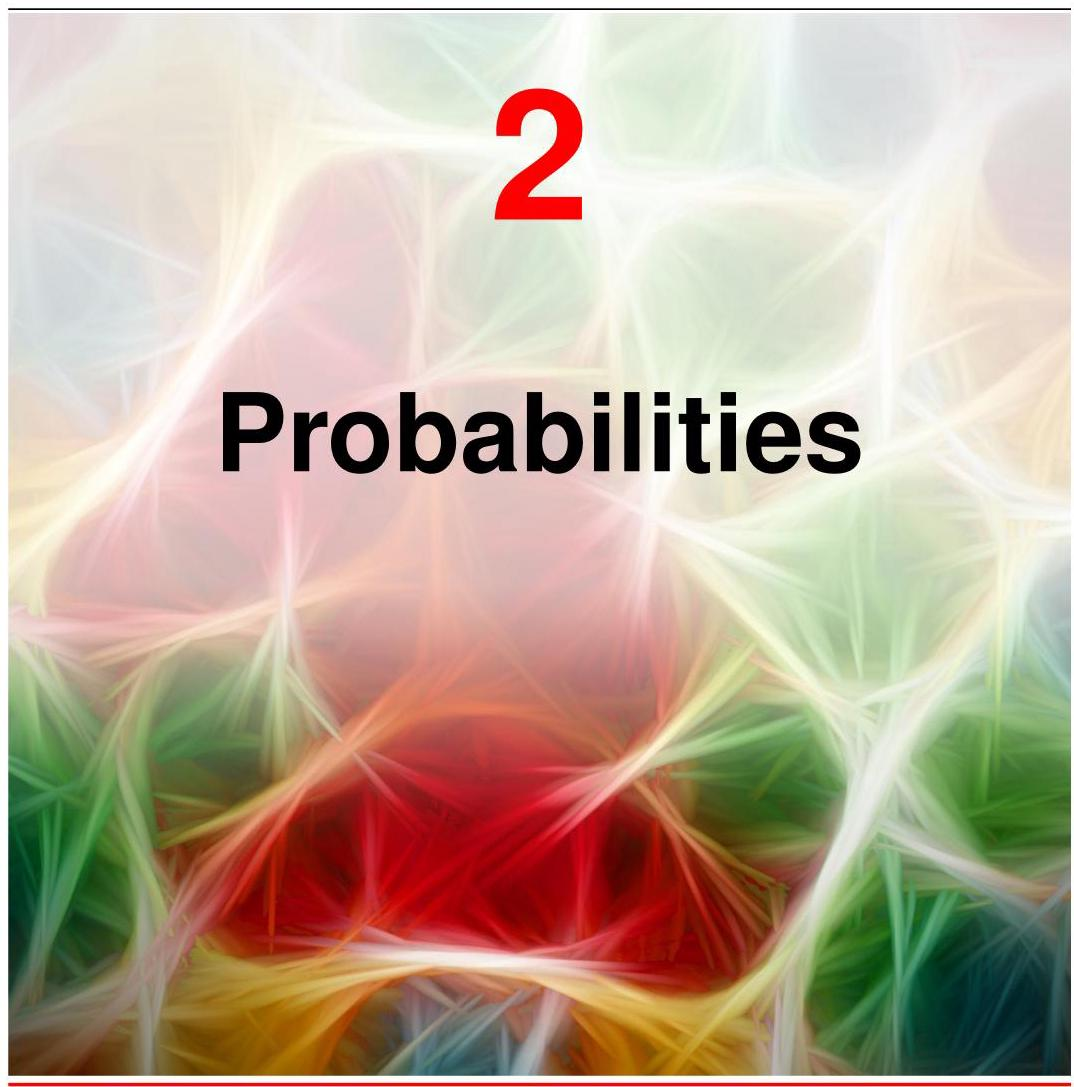
\includegraphics[max width=0.8\textwidth]{images/0194e279-9b28-703a-88f4-c3ac21e2010d_42_474_349_1074_1087_0.jpg}
\end{center}
\hspace*{3em} 

在机器学习的几乎所有应用中,我们都必须处理不确定性。例如,一个将皮肤病变图像分类为良性或恶性的系统在实践中永远无法达到完美的准确率。我们可以区分两种类型的不确定性。第一种是认知不确定性(源自希腊语 episteme,意为知识),有时也称为系统不确定性。它的产生是因为我们只能看到有限大小的数据集。例如,当我们观察到更多良性和恶性皮肤病变图像的示例时,我们就能更好地预测新示例的类别。然而,即使有一个无限大的数据集,由于第二种不确定性,即偶然不确定性(也称为内在或随机不确定性,有时简称为噪声),我们仍然无法达到完美的准确率。一般来说,噪声的产生是因为我们只能观察到关于世界的部分信息,因此,减少这种不确定性来源的一种方法是收集不同类型的数据。这一点在

\begin{center}
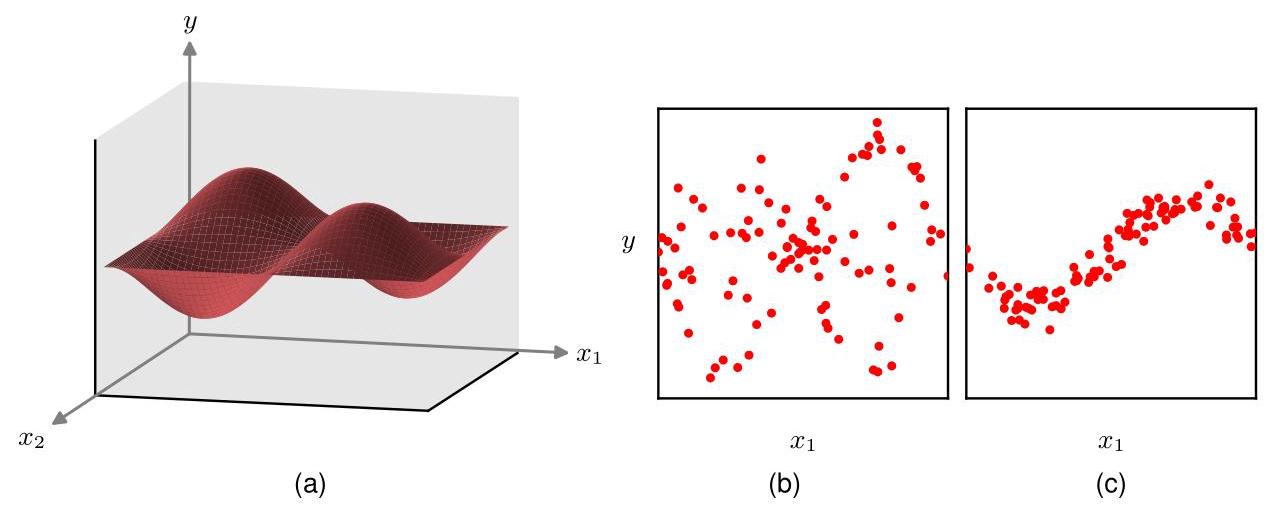
\includegraphics[max width=1.0\textwidth]{images/0194e279-9b28-703a-88f4-c3ac21e2010d_43_240_345_1276_509_0.jpg}
\end{center}
\hspace*{3em} 

图 2.1 简单正弦曲线回归问题向二维的扩展。(a) 函数 \(y\left( {{x}_{1},{x}_{2}}\right)  = \sin \left( {{2\pi }{x}_{1}}\right) \sin \left( {{2\pi }{x}_{2}}\right)\) 的绘图。通过选择 \({x}_{1}\) 和 \({x}_{2}\) 的值,计算 \(y\left( {{x}_{1},{x}_{2}}\right)\) 的相应值,然后添加高斯噪声来生成数据。(b) 100 个数据点的绘图,其中 \({x}_{2}\) 未被观察到,显示出高水平的噪声。(c) 100 个数据点的绘图,其中 \({x}_{2}\) 固定为值 \({x}_{2} = \frac{\pi }{2}\) ,模拟了能够同时测量 \({x}_{2}\) 和 \({x}_{1}\) 的效果,显示出低得多的噪声水平。

第 1.2 节通过图 2.1 中将正弦曲线示例扩展到二维的方式进行了说明。

作为一个实际例子,皮肤病变的活检样本比单独的图像提供的信息要多得多,并且可能会大大提高我们确定新病变是否为恶性的准确率。同时拥有图像和活检数据时,内在不确定性可能会非常小,并且通过收集大量的训练数据集,我们可能能够将系统不确定性降低到较低水平,从而高精度地预测病变的类别。

这两种不确定性都可以使用概率论的框架来处理,概率论为不确定性的量化和处理提供了一个一致的范式,因此构成了机器学习的核心基础之一。我们将看到,概率由两个简单的公式控制,即求和规则和乘积规则。当与决策理论相结合时,这些规则至少在原则上允许我们在给定所有可用信息的情况下做出最优预测,即使这些信息可能不完整或模糊不清。

\HRule

第 2.1 节

5.2 节

\HRule

概率的概念通常是根据可重复事件的频率来引入的。例如,考虑图 2.2 中所示的弯曲硬币,假设硬币的形状使得如果将其抛掷大量次数,它有 60\%的时间凹面朝上,因此有 40\%的时间凸面朝上。我们说凹面朝上的概率是 60\%或 0.6。严格来说,在这种情况下,概率是在无限多次“试验”或硬币抛掷的极限情况下定义的。因为硬币要么凹面朝上,要么凸面朝上,所以这些概率之和为 100\%或 1.0。这种根据可重复事件的频率来定义概率的方法是频率主义统计学观点的基础。

现在假设,尽管我们知道硬币凹面朝上的概率是 0.6,但我们不被允许看硬币本身,而且我们也不

图 2.2 知道哪一面是正面,哪一面是反面。如果被要求对硬币抛掷时是正面朝上还是反面朝上进行下注,那么根据对称性,我们的下注应该基于正面出现的概率为 0.5 这一假设,而且更仔细的分析表明,在没有任何额外信息的情况下,这确实是合理的选择。在这里,我们使用概率的意义比单纯的事件频率更广泛。硬币的凸面是正面还是反面本身并不是一个可重复的事件,它只是未知的。将概率用作不确定性的量化是贝叶斯观点,并且更具一般性,因为它将频率主义概率作为一种特殊情况包含在内。如果我们得到一系列硬币抛掷的结果,我们可以通过使用贝叶斯推理来了解硬币的哪一面是正面。我们观察到的结果越多,我们对硬币哪一面是哪一面的不确定性就越低。

\begin{center}
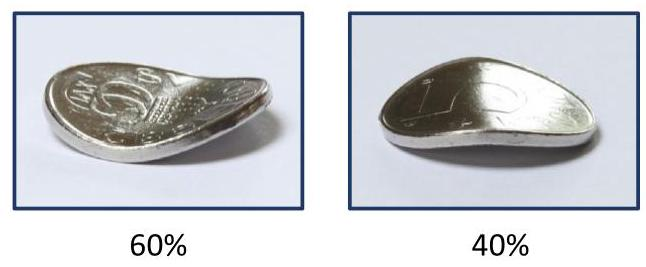
\includegraphics[max width=0.5\textwidth]{images/0194e279-9b28-703a-88f4-c3ac21e2010d_44_902_348_646_267_0.jpg}
\end{center}
\hspace*{3em} 

2 概率既可以被视为与可重复事件相关的频率,也可以被视为不确定性的量化。如文中所讨论的,弯曲的硬币可以用来阐明这种区别。

\HRule

2.6 节

练习 2.40

\HRule

在非正式地引入了概率的概念之后,我们现在转向对概率进行更详细的探讨,并讨论如何定量地使用它们。本章其余部分所阐述的概念将为本书中讨论的许多主题奠定核心基础。

\section*{2.1. 概率规则}

在本节中,我们将推导出两条支配概率行为的简单规则。然而,尽管这些规则看似简单,但事实将证明它们非常强大且应用广泛。我们将首先通过引入一个简单的例子来引出概率规则。

\section*{2.1.1 一个医学筛查示例}

考虑对人群进行筛查以实现癌症早期检测的问题,假设该人群中有 1\% 的人实际患有癌症。理想情况下,我们的癌症检测对于任何患有癌症的人都会给出阳性结果,对于任何未患癌症的人都会给出阴性结果。然而,检测并非完美无缺,因此我们假设,当对未患癌症的人进行检测时,其中 3\% 的人检测结果会呈阳性。这些被称为假阳性。同样,当对患有癌症的人进行检测时,其中 10\% 的人检测结果会呈阴性。这些被称为假阴性。各种错误率如图 2.3 所示。

根据这些信息,我们可能会提出以下问题:(1)“如果我们对人群进行筛查,某人检测呈阳性的概率是多少?”(2)“如果某人检测结果呈阳性,他们实际患有癌症的概率是多少?”我们可以通过详细分析癌症筛查案例来回答这些问题。然而,我们将暂停对这个具体例子的讨论,首先推导概率的一般规则,即概率的加法规则和乘法规则。然后,我们将通过回答这两个问题来说明这些规则的应用。

\begin{center}
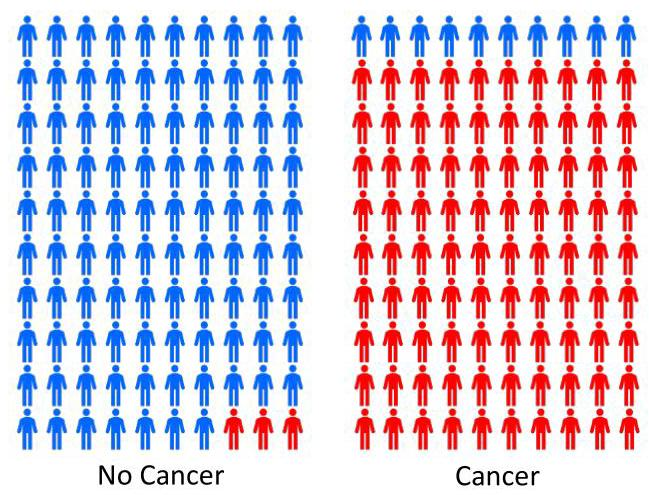
\includegraphics[max width=0.5\textwidth]{images/0194e279-9b28-703a-88f4-c3ac21e2010d_45_904_342_649_495_0.jpg}
\end{center}
\hspace*{3em} 

图 2.3 癌症检测准确性的说明。在左侧所示的每一百名接受检测但未患癌症的人中,平均有三人检测呈阳性。对于右侧所示的患有癌症的人,每一百名接受检测的人中,平均有 90 人检测呈阳性。

\section*{2.1.2 加法规则和乘法规则}

为了推导概率规则,考虑图 2.4 中所示的稍微更一般的例子,涉及两个变量 \(X\) 和 \(Y\) 。在我们的癌症例子中, \(X\) 可以表示是否患有癌症, \(Y\) 可以是一个表示检测结果的变量。由于这些变量的值在不同人之间的变化方式通常是未知的,它们被称为随机变量或随机变量。我们假设 \(X\) 可以取任何 \({x}_{i}\) 的值,其中 \(i = 1,\ldots ,L\) ,并且 \(Y\) 可以取 \({y}_{j}\) 的值,其中 \(j = 1,\ldots ,M\) 。考虑总共进行 \(N\) 次试验,在这些试验中我们同时对变量 \(X\) 和 \(Y\) 进行采样,并且让 \(X = {x}_{i}\) 和 \(Y = {y}_{j}\) 同时出现的试验次数为 \({n}_{ij}\) 。此外,让 \(X\) 取 \({x}_{i}\) 值(无论 \(Y\) 取何值)的试验次数用 \({c}_{i}\) 表示,类似地,让 \(Y\) 取 \({y}_{j}\) 值的试验次数用 \({r}_{j}\) 表示。

\(X\) 取 \({x}_{i}\) 值且 \(Y\) 取 \({y}_{j}\) 值的概率写作 \(p\left( {X = {x}_{i},Y = {y}_{j}}\right)\) ,并称为 \(X = {x}_{i}\) 和 \(Y = {y}_{j}\) 的联合概率。它由落在单元格 \(i,j\) 中的点数占总点数的比例给出,因此

\[
p\left( {X = {x}_{i},Y = {y}_{j}}\right)  = \frac{{n}_{ij}}{N}. \tag{2.1}
\]

这里我们隐含地考虑极限 \(N \rightarrow  \infty\) 。类似地, \(X\) 取 \({x}_{i}\) 值而不考虑 \(Y\) 值的概率写作 \(p\left( {X = {x}_{i}}\right)\) ,并且是

图 2.4 我们可以通过考虑一个随机变量 \(X\) 来推导概率的加法规则和乘法规则,该随机变量取值为 \(\left\{  {x}_{i}\right\}\) ,其中 \(i = 1,\ldots ,L\) ,以及第二个随机变量 \(Y\) ,其取值为 \(\left\{  {y}_{j}\right\}\) ,其中 \(j =\)  \(1,\ldots ,M\) 。在这个示例中,我们有 \(L = 5\) 和 \(M = 3\) 。如果我们考虑这些变量的实例总数 \(N\) ,那么我们用 \({n}_{ij}\) 表示 \(X = {x}_{i}\) 且 \(Y = {y}_{j}\) 的实例数量,这是数组中相应单元格的实例数量。对应于 \(X = {x}_{i}\) 的列 \(i\) 中的实例数量用 \({c}_{i}\) 表示,对应于 \(Y = {y}_{j}\) 的行 \(j\) 中的实例数量用 \({r}_{j}\) 表示。由落在列 \(i\) 中的点的总数的比例给出,因此

\[
p\left( {X = {x}_{i}}\right)  = \frac{{c}_{i}}{N}. \tag{2.2}
\]

\begin{center}
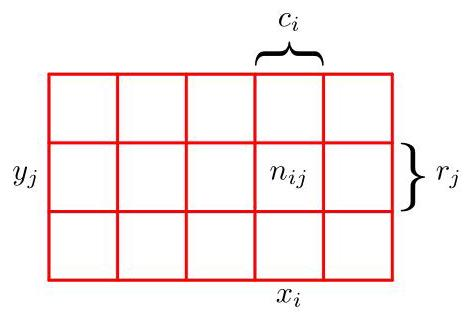
\includegraphics[max width=0.3\textwidth]{images/0194e279-9b28-703a-88f4-c3ac21e2010d_46_1083_344_466_312_0.jpg}
\end{center}
\hspace*{3em} 

由于 \(\mathop{\sum }\limits_{i}{c}_{i} = N\) ,我们可以看到

\[
\mathop{\sum }\limits_{{i = 1}}^{L}p\left( {X = {x}_{i}}\right)  = 1 \tag{2.3}
\]

因此,概率如要求的那样总和为 1。因为图 2.4 中列 \(i\) 的实例数量恰好是该列中每个单元格的实例数量之和,所以我们有 \({c}_{i} = \mathop{\sum }\limits_{j}{n}_{ij}\) ,因此,根据式(2.1)和式(2.2),我们得到

\[
p\left( {X = {x}_{i}}\right)  = \mathop{\sum }\limits_{{j = 1}}^{M}p\left( {X = {x}_{i},Y = {y}_{j}}\right) , \tag{2.4}
\]

这就是概率的加法规则。注意, \(p\left( {X = {x}_{i}}\right)\) 有时被称为边缘概率,它是通过对其他变量(在这种情况下是 \(Y\) )进行边缘化或求和得到的。

如果我们只考虑 \(X = {x}_{i}\) 的那些实例,那么在这些实例中 \(Y = {y}_{j}\) 的比例记为 \(p\left( {Y = {y}_{j} \mid  X = {x}_{i}}\right)\) ,并称为在 \(X = {x}_{i}\) 给定的条件下 \(Y = {y}_{j}\) 的条件概率。它是通过找出列 \(i\) 中落在单元格 \(i,j\) 中的点的比例得到的,因此由下式给出

\[
p\left( {Y = {y}_{j} \mid  X = {x}_{i}}\right)  = \frac{{n}_{ij}}{{c}_{i}}. \tag{2.5}
\]

对 \(j\) 对等式两边求和,并使用 \(\mathop{\sum }\limits_{j}{n}_{ij} = {c}_{i}\) ,我们得到

\[
\mathop{\sum }\limits_{{j = 1}}^{M}p\left( {Y = {y}_{j} \mid  X = {x}_{i}}\right)  = 1 \tag{2.6}
\]

表明条件概率已被正确归一化。从 (2.1)、(2.2) 和 (2.5),我们可以推导出以下关系:

\[
p\left( {X = {x}_{i},Y = {y}_{j}}\right)  = \frac{{n}_{ij}}{N} = \frac{{n}_{ij}}{{c}_{i}} \cdot  \frac{{c}_{i}}{N}
\]

\[
= p\left( {Y = {y}_{j} \mid  X = {x}_{i}}\right) p\left( {X = {x}_{i}}\right) \text{ , } \tag{2.7}
\]

这就是概率的乘法规则。

到目前为止,我们一直非常谨慎地区分随机变量(如 \(X\) )和随机变量所能取的值(例如 \({x}_{i}\) )。因此, \(X\) 取 \({x}_{i}\) 这个值的概率表示为 \(p\left( {X = {x}_{i}}\right)\) 。虽然这有助于避免歧义,但会导致符号表示相当繁琐,而且在很多情况下并不需要如此拘泥细节。相反,只要上下文能明确其含义,我们可以简单地用 \(p\left( X\right)\) 表示随机变量 \(X\) 的分布,或者用 \(p\left( {x}_{i}\right)\) 表示在特定值 \({x}_{i}\) 处的分布。

使用这种更简洁的符号表示,我们可以将概率论的两个基本规则写成以下形式:

\[
\text{ sum rule }\;p\left( X\right)  = \mathop{\sum }\limits_{Y}p\left( {X,Y}\right)  \tag{2.8}
\]

\[
\text{ product rule }\;p\left( {X,Y}\right)  = p\left( {Y \mid  X}\right) p\left( X\right) \text{ . } \tag{2.9}
\]

这里 \(p\left( {X,Y}\right)\) 是联合概率,表述为 “ \(X\) 和 \(Y\) 的概率”。类似地,量 \(p\left( {Y \mid  X}\right)\) 是条件概率,表述为 “在 \(X\) 给定的条件下 \(Y\) 的概率”。最后,量 \(p\left( X\right)\) 是边缘概率,简单表述为 “ \(X\) 的概率”。这两条简单的规则构成了我们在本书中使用的所有概率工具的基础。

\section*{2.1.3 贝叶斯定理}

根据乘积法则,结合对称性 \(p\left( {X,Y}\right)  = p\left( {Y,X}\right)\) ,我们可以立即得到条件概率之间的以下关系:

\[
p\left( {Y \mid  X}\right)  = \frac{p\left( {X \mid  Y}\right) p\left( Y\right) }{p\left( X\right) }, \tag{2.10}
\]

这被称为贝叶斯定理,它在机器学习中起着重要作用。请注意贝叶斯定理是如何将方程左侧的条件分布 \(p\left( {Y \mid  X}\right)\) 与右侧的 “反向” 条件分布 \(p\left( {X \mid  Y}\right)\) 联系起来的。利用求和法则,贝叶斯定理中的分母可以用分子中出现的量来表示:

\[
p\left( X\right)  = \mathop{\sum }\limits_{Y}p\left( {X \mid  Y}\right) p\left( Y\right) . \tag{2.11}
\]

因此,我们可以将贝叶斯定理中的分母视为一个归一化常数,用于确保 (2.10) 式左侧的条件概率分布在 \(Y\) 的所有取值上的和等于 1。

\begin{center}
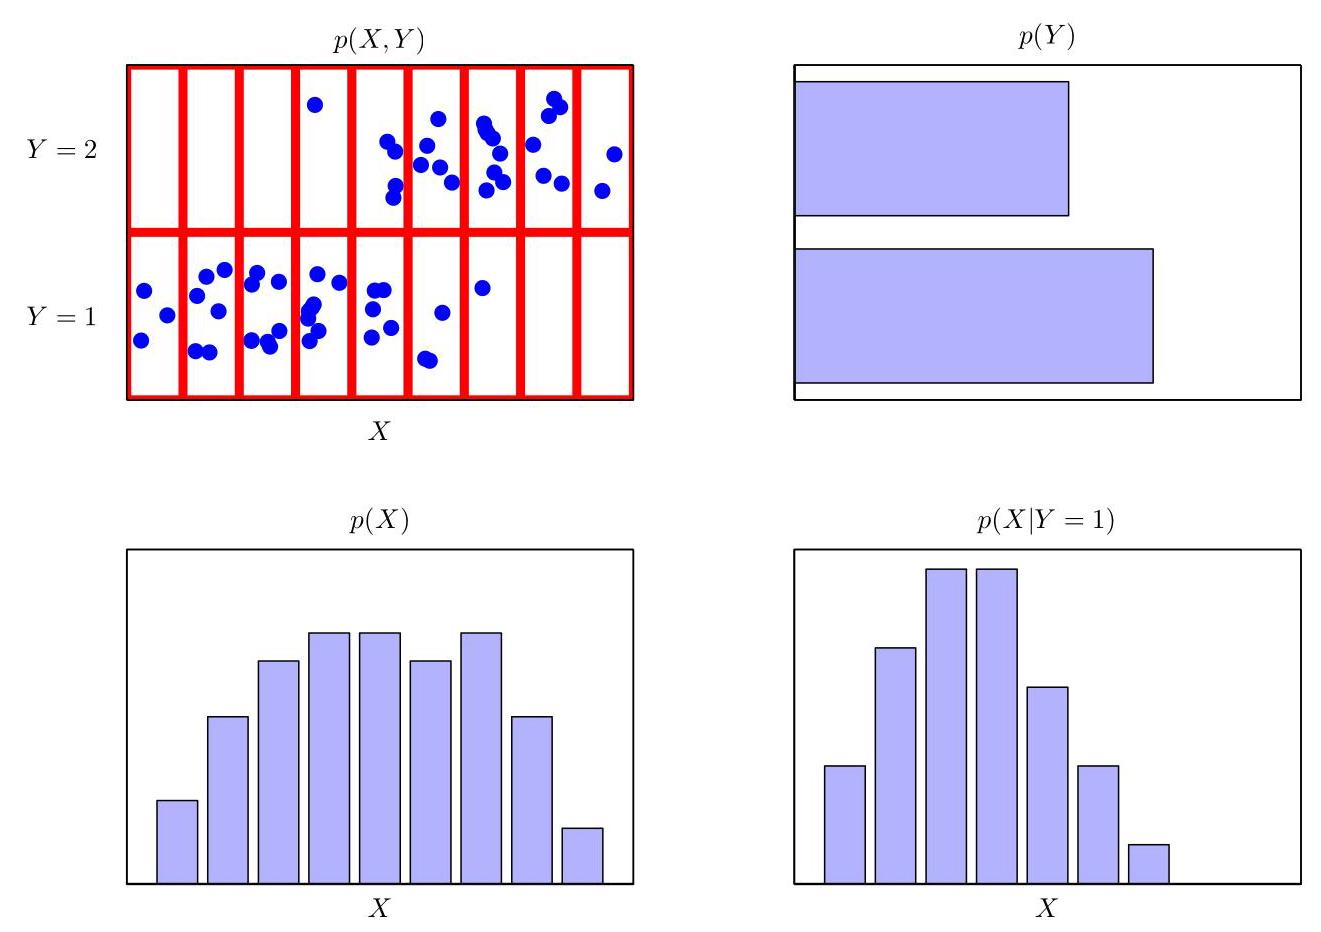
\includegraphics[max width=1.0\textwidth]{images/0194e279-9b28-703a-88f4-c3ac21e2010d_48_213_376_1321_932_0.jpg}
\end{center}
\hspace*{3em} 

图 2.5 展示了两个变量的分布, \(X\) 有 9 种可能的取值, \(Y\) 有 2 种可能的取值。左上图显示了从这些变量的联合概率分布中抽取的 60 个点的样本。其余的图展示了边缘分布 \(p\left( X\right)\) 和 \(p\left( Y\right)\) 的直方图估计,以及与左上图中底行对应的条件分布 \(p\left( {X \mid  Y = 1}\right)\) 。

在图 2.5 中,我们展示了一个涉及两个变量联合分布的简单示例,以说明边缘分布和条件分布的概念。这里从联合分布中抽取了 \(N = {60}\) 个数据点的有限样本,并显示在左上方。右上方是具有 \(Y\) 的两个值的数据点比例的直方图。根据概率的定义,当样本大小为 \(N \rightarrow  \infty\) 时,这些比例将等于相应的概率 \(p\left( Y\right)\) 。我们可以将直方图视为一种在仅给定从该分布中抽取的有限个点的情况下对概率分布进行建模的简单方法。图 2.5 中的其余两个图展示了 \(p\left( X\right)\) 和 \(p\left( {X \mid  Y = 1}\right)\) 的相应直方图估计。

\HRule

第 3.5.1 节

\HRule

\section*{2.1.4 重新审视医学筛查}

现在让我们回到癌症筛查的例子,并应用概率的求和与乘积规则来回答我们的两个问题。为了清晰起见,在分析这个例子时,我们将再次明确区分随机变量及其取值。我们用变量 \(C\) 表示是否患有癌症,它可以取两个值: \(C = 0\) 对应 “无癌症”, \(C = 1\) 对应 “癌症”。我们假设人群中每一百人中有一人患有癌症,因此我们有

\[
p\left( {C = 1}\right)  = 1/{100} \tag{2.12}
\]

\[
p\left( {C = 0}\right)  = {99}/{100}, \tag{2.13}
\]

分别地。注意,这些满足 \(p\left( {C = 0}\right)  + p\left( {C = 1}\right)  = 1\) 。

现在让我们引入第二个随机变量 \(T\) 来表示筛查测试的结果,其中 \(T = 1\) 表示阳性结果,表明患有癌症, \(T = 0\) 表示阴性结果,表明没有癌症。如图 2.3 所示,我们知道对于患有癌症的人,测试结果为阳性的概率是 90\%,而对于没有癌症的人,测试结果为阳性的概率是 3\%。因此,我们可以写出所有四个条件概率:

\[
p\left( {T = 1 \mid  C = 1}\right)  = {90}/{100} \tag{2.14}
\]

\[
p\left( {T = 0 \mid  C = 1}\right)  = {10}/{100} \tag{2.15}
\]

\[
p\left( {T = 1 \mid  C = 0}\right)  = 3/{100} \tag{2.16}
\]

\[
p\left( {T = 0 \mid  C = 0}\right)  = {97}/{100}\text{ . } \tag{2.17}
\]

同样,注意这些概率是归一化的,使得

\[
p\left( {T = 1 \mid  C = 1}\right)  + p\left( {T = 0 \mid  C = 1}\right)  = 1 \tag{2.18}
\]

并且类似地

\[
p\left( {T = 1 \mid  C = 0}\right)  + p\left( {T = 0 \mid  C = 0}\right)  = 1. \tag{2.19}
\]

现在,我们可以使用概率的加法规则和乘法规则来回答第一个问题,并评估随机接受检测的人检测结果呈阳性的总体概率:

\[
p\left( {T = 1}\right)  = p\left( {T = 1 \mid  C = 0}\right) p\left( {C = 0}\right)  + p\left( {T = 1 \mid  C = 1}\right) p\left( {C = 1}\right)
\]

\[
= \frac{3}{100} \times  \frac{99}{100} + \frac{90}{100} \times  \frac{1}{100} = \frac{387}{{10},{000}} = {0.0387}. \tag{2.20}
\]

我们发现,如果随机对一个人进行检测,即使他们实际患癌症的概率为 1\%,检测结果呈阳性的概率也约为 4\%。由此,根据加法规则可知, \(p\left( {T = 0}\right)  = 1 - {387}/{10},{000} =\)  \({9613}/{10},{000} = {0.9613}\) ,因此,他们未患癌症的概率约为 \({96}\%\) 。

现在考虑我们的第二个问题,这也是接受筛查的人特别关心的问题:如果检测结果呈阳性,这个人患癌症的概率是多少?这要求我们评估在检测结果已知的条件下患癌症的概率,而式(2.14)至式(2.17)中的概率给出的是在已知一个人是否患癌症的条件下检测结果的概率分布。我们可以使用贝叶斯定理(2.10)来解决反转条件概率的问题,得到

\[
p\left( {C = 1 \mid  T = 1}\right)  = \frac{p\left( {T = 1 \mid  C = 1}\right) p\left( {C = 1}\right) }{p\left( {T = 1}\right) } \tag{2.21}
\]

\[
= \frac{90}{100} \times  \frac{1}{100} \times  \frac{{10},{000}}{387} = \frac{90}{387} \simeq  {0.23} \tag{2.22}
\]

因此,如果随机对一个人进行检测且检测结果呈阳性,那么他们实际患癌症的概率为 23\%。根据加法规则,可得 \(p(C =\)  \(0 \mid  T = 1) = 1 - {90}/{387} = {297}/{387} \simeq  {0.77}\) ,即他们未患癌症的概率为 \({77}\%\) 。

\section*{2.1.5 先验概率和后验概率}

我们可以用癌症筛查的例子对贝叶斯定理给出如下重要解释。如果在某人接受检测之前,我们被问及这个人是否可能患癌症,那么我们所能获得的最完整信息由概率 \(p\left( C\right)\) 给出。我们将其称为先验概率,因为这是在我们观察到检测结果之前就已知的概率。一旦得知这个人的检测结果呈阳性,我们就可以使用贝叶斯定理来计算概率 \(p\left( {C \mid  T}\right)\) ,我们将其称为后验概率,因为这是在我们观察到检测结果 \(T\) 之后得到的概率。

在这个例子中,患癌症的先验概率是 1\%。然而,一旦我们观察到检测结果为阳性,我们会发现患癌症的后验概率现在是 23\%,这是一个显著更高的患癌概率,正如我们直观预期的那样。然而,我们注意到,即使从图 2.3 来看该检测似乎相当“准确”,检测结果为阳性的人实际患癌症的概率仍然只有 23\%。这个结论在很多人看来有悖直觉。原因与患癌症的先验概率较低有关。尽管该检测提供了患癌的有力证据,但必须使用贝叶斯定理将其与先验概率相结合,才能得出正确的后验概率。

\HRule

练习 2.1

\HRule

\section*{2.1.6 独立变量}

最后,如果两个变量的联合分布可以分解为边缘分布的乘积,即 \(p\left( {X,Y}\right)  = p\left( X\right) p\left( Y\right)\) ,那么就称 \(X\) 和 \(Y\) 是独立的。独立事件的一个例子是连续抛硬币。根据乘法规则,我们可以得到 \(p\left( {Y \mid  X}\right)  = p\left( Y\right)\) ,因此给定 \(X\) 时 \(Y\) 的条件分布确实与 \(X\) 的值无关。在我们的癌症筛查例子中,如果检测结果为阳性的概率与一个人是否患癌症无关,那么 \(p\left( {T \mid  C}\right)  = p\left( T\right)\) ,这意味着根据贝叶斯定理(2.10)我们有 \(p\left( {C \mid  T}\right)  = p\left( C\right)\) ,因此观察检测结果并不会改变患癌症的概率。当然,这样的检测是没有用的,因为检测结果无法告诉我们一个人是否患癌症。

\begin{center}
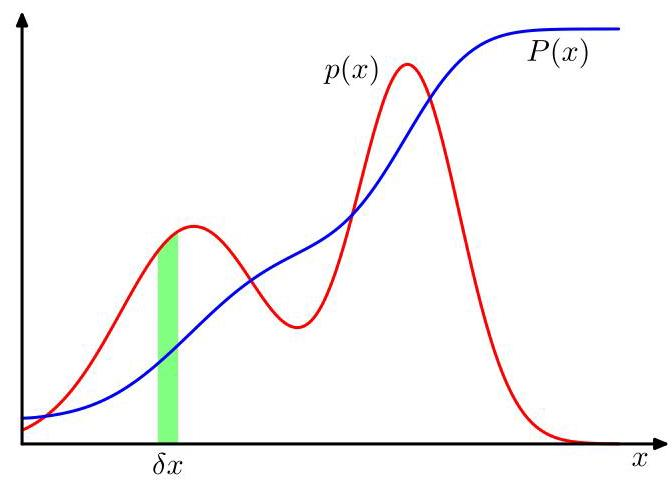
\includegraphics[max width=0.5\textwidth]{images/0194e279-9b28-703a-88f4-c3ac21e2010d_51_879_344_672_483_0.jpg}
\end{center}
\hspace*{3em} 

图 2.6 离散变量的概率概念可以扩展到连续变量 \(x\) 上的概率密度 \(p\left( x\right)\) ,使得 \(x\) 落在区间 \(\left( {x,x + {\delta x}}\right)\) 内的概率由 \(p\left( x\right) {\delta x}\) 给出,其中 \({\delta x} \rightarrow  0\) 。概率密度可以表示为累积分布函数 \(P\left( x\right)\) 的导数。

\section*{2.2. 概率密度}

除了考虑在离散值集上定义的概率之外,我们还希望考虑关于连续变量的概率。例如,我们可能希望预测给患者使用的药物剂量。由于这种预测存在不确定性,我们希望量化这种不确定性,并且同样可以利用概率。然而,我们不能简单地直接应用到目前为止所讨论的概率概念,因为以无限精度观察连续变量的特定值的概率实际上将为零。相反,我们需要引入概率密度的概念。在这里,我们将仅限于进行相对非正式的讨论。

我们定义连续变量 \(x\) 上的概率密度 \(p\left( x\right)\) ,使得 \(x\) 落在区间 \(\left( {x,x + {\delta x}}\right)\) 内的概率由 \(p\left( x\right) {\delta x}\) 给出,其中 \({\delta x} \rightarrow  0\) 。这在图 2.6 中进行了说明。那么 \(x\) 落在区间 \(\left( {a,b}\right)\) 内的概率由下式给出

\[
p\left( {x \in  \left( {a,b}\right) }\right)  = {\int }_{a}^{b}p\left( x\right) \mathrm{d}x. \tag{2.23}
\]

由于概率是非负的,并且由于 \(x\) 的值必定位于实轴上的某个位置,概率密度 \(p\left( x\right)\) 必须满足两个条件

\[
p\left( x\right)  \geq  0 \tag{2.24}
\]

\[
{\int }_{-\infty }^{\infty }p\left( x\right) \mathrm{d}x = 1 \tag{2.25}
\]

\(x\) 落在区间 \(\left( {-\infty ,z}\right)\) 内的概率由累积分布函数给出,其定义为

\[
P\left( z\right)  = {\int }_{-\infty }^{z}p\left( x\right) \mathrm{d}x \tag{2.26}
\]

如图 2.6 所示,它满足 \({P}^{\prime }\left( x\right)  = p\left( x\right)\) 。

如果我们有几个连续变量 \({x}_{1},\ldots ,{x}_{D}\) ,用向量 \(\mathbf{x}\) 统一表示,那么我们可以定义一个联合概率密度 \(p\left( \mathbf{x}\right)  = p\left( {{x}_{1},\ldots ,{x}_{D}}\right)\) ,使得 \(\mathrm{x}\) 落在包含点 \(\mathrm{x}\) 的无穷小体积 \(\delta \mathrm{x}\) 内的概率由 \(p\left( \mathbf{x}\right) \delta \mathbf{x}\) 给出。这个多元概率密度必须满足

\[
p\left( \mathbf{x}\right)  \geq  0 \tag{2.27}
\]

\[
\int p\left( \mathbf{x}\right) \mathrm{d}\mathbf{x} = 1 \tag{2.28}
\]

其中积分是在整个 \(\mathbf{x}\) 空间上进行的。更一般地,我们还可以考虑离散变量和连续变量组合的联合概率分布。

概率的求和规则和乘积规则,以及贝叶斯定理,同样适用于概率密度以及离散变量和连续变量的组合。如果 \(\mathbf{x}\) 和 \(\mathbf{y}\) 是两个实变量,那么求和规则和乘积规则的形式为

\[
\text{ sum rule }\;p\left( \mathbf{x}\right)  = \int p\left( {\mathbf{x},\mathbf{y}}\right) \mathrm{d}\mathbf{y} \tag{2.29}
\]

\[
\text{ product rule }\;p\left( {\mathbf{x},\mathbf{y}}\right)  = p\left( {\mathbf{y} \mid  \mathbf{x}}\right) p\left( \mathbf{x}\right) \text{ . } \tag{2.30}
\]

类似地,贝叶斯定理可以写成如下形式

\[
p\left( {\mathbf{y} \mid  \mathbf{x}}\right)  = \frac{p\left( {\mathbf{x} \mid  \mathbf{y}}\right) p\left( \mathbf{y}\right) }{p\left( \mathbf{x}\right) } \tag{2.31}
\]

其中分母由下式给出

\[
p\left( \mathbf{x}\right)  = \int p\left( {\mathbf{x} \mid  \mathbf{y}}\right) p\left( \mathbf{y}\right) \mathrm{d}\mathbf{y}. \tag{2.32}
\]

对连续变量的求和规则和乘积规则进行正式的证明需要用到数学中一个称为测度论的分支(Feller,1966),这超出了本书的范围。然而,我们可以通过将每个实变量划分为宽度为 \(\Delta\) 的区间,并考虑这些区间上的离散概率分布,来非正式地理解其有效性。取极限 \(\Delta  \rightarrow  0\) 时,求和就变成了积分,从而得到所需的结果。

\section*{2.2.1 示例分布}

有许多形式的概率密度被广泛使用,它们本身就很重要,同时也是构建更复杂概率模型的基础。最简单的形式是 \(p\left( x\right)\) 为常数,与 \(x\) 无关,但这无法进行归一化,因为 (2.28) 中的积分会发散。无法归一化的分布称为非正则分布。然而,我们可以有在有限区域(例如 \(\left( {c,d}\right)\) )内为常数,在其他地方为零的均匀分布,在这种情况下,(2.28) 意味着

\[
p\left( x\right)  = 1/\left( {d - c}\right) ,\;x \in  \left( {c,d}\right) . \tag{2.33}
\]

\begin{center}
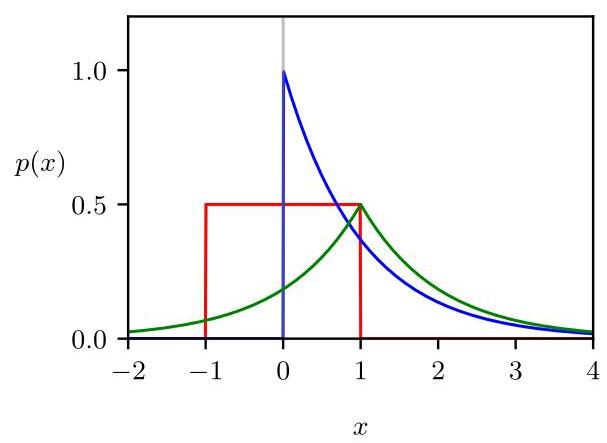
\includegraphics[max width=0.4\textwidth]{images/0194e279-9b28-703a-88f4-c3ac21e2010d_53_944_343_607_443_0.jpg}
\end{center}
\hspace*{3em} 

图 2.7 绘制了在区间 \(\left( {-1,1}\right)\) 上的均匀分布(红色)、参数为 \(\lambda  = 1\) 的指数分布(蓝色)以及参数为 \(\mu  = 1\) 和 \(\gamma  = 1\) 的拉普拉斯分布(绿色)。

另一种简单的密度形式是由下式给出的指数分布

\[
p\left( {x \mid  \lambda }\right)  = \lambda \exp \left( {-{\lambda x}}\right) ,\;x \geq  0. \tag{2.34}
\]

指数分布的一种变体,即拉普拉斯分布,允许将峰值移动到位置 \(\mu\) ,其表达式为

\[
p\left( {x \mid  \mu ,\gamma }\right)  = \frac{1}{2\gamma }\exp \left( {-\frac{\left| x - \mu \right| }{\gamma }}\right) . \tag{2.35}
\]

常数分布、指数分布和拉普拉斯分布如图 2.7 所示。

另一个重要的分布是狄拉克δ函数,其表示为

\[
p\left( {x \mid  \mu }\right)  = \delta \left( {x - \mu }\right) . \tag{2.36}
\]

除了在 \(x = \mu\) 处,该函数在其他地方都被定义为零,并且根据 (2.28) 式,它具有积分结果为 1 的性质。通俗地说,我们可以将其看作是位于 \(x = \mu\) 处的一个无限窄且无限高的尖峰,其面积为 1。最后,如果我们有一组关于 \(x\) 的有限观测值 \(\mathcal{D} = \left\{  {{x}_{1},\ldots ,{x}_{N}}\right\}\) ,那么我们可以使用狄拉克δ函数来构造如下的经验分布

\[
p\left( {x \mid  \mathcal{D}}\right)  = \frac{1}{N}\mathop{\sum }\limits_{{n = 1}}^{N}\delta \left( {x - {x}_{n}}\right) , \tag{2.37}
\]

该分布由以每个数据点为中心的狄拉克δ函数组成。由 (2.37) 式定义的概率密度函数的积分结果符合要求,为 1。

\HRule

练习 2.6

\HRule

\section*{2.2.2 期望和协方差}

涉及概率的最重要运算之一是求函数的加权平均值。在概率分布 \(p\left( x\right)\) 下,某个函数 \(f\left( x\right)\) 的加权平均值称为 \(f\left( x\right)\) 的期望,用 \(\mathbb{E}\left\lbrack  f\right\rbrack\) 表示。对于离散分布,它可以通过对 \(f\left( x\right)\) 的所有可能取值求和得到

其形式为

\[
\mathbb{E}\left\lbrack  f\right\rbrack   = \mathop{\sum }\limits_{x}p\left( x\right) f\left( x\right)  \tag{2.38}
\]

其中平均值由 \(x\) 不同值的相对概率加权得到。对于连续变量,期望用相对于相应概率密度的积分来表示:

\[
\mathbb{E}\left\lbrack  f\right\rbrack   = \int p\left( x\right) f\left( x\right) \mathrm{d}x. \tag{2.39}
\]

在这两种情况下,如果我们得到从概率分布或概率密度中抽取的有限个点 \(N\) ,那么期望可以近似为这些点上的有限和:

\[
\mathbb{E}\left\lbrack  f\right\rbrack   \simeq  \frac{1}{N}\mathop{\sum }\limits_{{n = 1}}^{N}f\left( {x}_{n}\right) . \tag{2.40}
\]

\HRule

练习 2.7

\HRule

在极限 \(N \rightarrow  \infty\) 下,(2.40) 中的近似变得精确。

有时我们会考虑多个变量的函数的期望,在这种情况下,我们可以使用下标来表示对哪个变量求平均,例如

\[
{\mathbb{E}}_{x}\left\lbrack  {f\left( {x,y}\right) }\right\rbrack   \tag{2.41}
\]

表示函数 \(f\left( {x,y}\right)\) 相对于 \(x\) 的分布的平均值。注意 \({\mathbb{E}}_{x}\left\lbrack  {f\left( {x,y}\right) }\right\rbrack\) 将是 \(y\) 的函数。

我们还可以考虑关于条件分布的条件期望,即

\[
{\mathbb{E}}_{x}\left\lbrack  {f \mid  y}\right\rbrack   = \mathop{\sum }\limits_{x}p\left( {x \mid  y}\right) f\left( x\right) , \tag{2.42}
\]

这也是 \(y\) 的一个函数。对于连续变量,条件期望

具有如下形式

\[
{\mathbb{E}}_{x}\left\lbrack  {f \mid  y}\right\rbrack   = \int p\left( {x \mid  y}\right) f\left( x\right) \mathrm{d}x. \tag{2.43}
\]

\(f\left( x\right)\) 的方差定义为

\[
\operatorname{var}\left\lbrack  f\right\rbrack   = \mathbb{E}\left\lbrack  {\left( f\left( x\right)  - \mathbb{E}\left\lbrack  f\left( x\right) \right\rbrack  \right) }^{2}\right\rbrack   \tag{2.44}
\]

它衡量了 \(f\left( x\right)\) 相对于其均值 \(\mathbb{E}\left\lbrack  {f\left( x\right) }\right\rbrack\) 的变化程度。将平方项展开,我们可以看到方差也可以用 \(f\left( x\right)\) 和 \(f{\left( x\right) }^{2}\) 的期望来表示:

\[
\operatorname{var}\left\lbrack  f\right\rbrack   = \mathbb{E}\left\lbrack  {f{\left( x\right) }^{2}}\right\rbrack   - \mathbb{E}{\left\lbrack  f\left( x\right) \right\rbrack  }^{2}. \tag{2.45}
\]

\HRule

练习 2.8

\HRule

特别地,我们可以考虑变量 \(x\) 本身的方差,其表达式为

\[
\operatorname{var}\left\lbrack  x\right\rbrack   = \mathbb{E}\left\lbrack  {x}^{2}\right\rbrack   - \mathbb{E}{\left\lbrack  x\right\rbrack  }^{2}. \tag{2.46}
\]

对于两个随机变量 \(x\) 和 \(y\) ,协方差衡量了这两个变量一起变化的程度,其定义为

\[
\operatorname{cov}\left\lbrack  {x,y}\right\rbrack   = {\mathbb{E}}_{x,y}\left\lbrack  {\{ x - \mathbb{E}\left\lbrack  x\right\rbrack  \} \{ y - \mathbb{E}\left\lbrack  y\right\rbrack  \} }\right\rbrack
\]

\[
= {\mathbb{E}}_{x,y}\left\lbrack  {xy}\right\rbrack   - \mathbb{E}\left\lbrack  x\right\rbrack  \mathbb{E}\left\lbrack  y\right\rbrack  \text{ . } \tag{2.47}
\]

\begin{center}
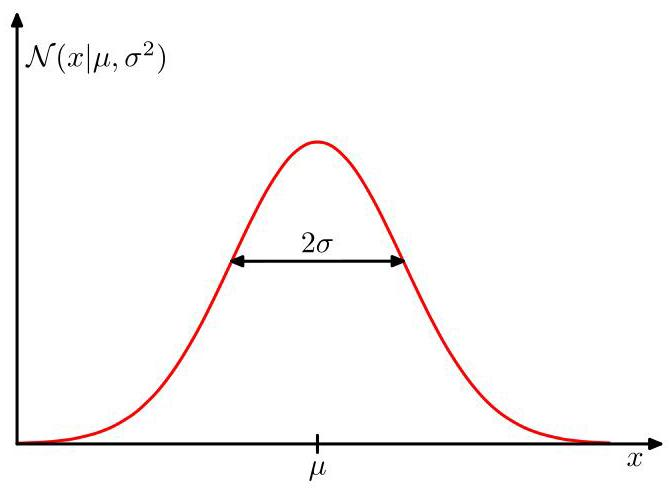
\includegraphics[max width=0.5\textwidth]{images/0194e279-9b28-703a-88f4-c3ac21e2010d_55_884_344_669_490_0.jpg}
\end{center}
\hspace*{3em} 

图 2.8 展示了单个连续变量 \(x\) 的高斯分布曲线,其中标注了均值 \(\mu\) 和标准差 \(\sigma\) 。

\HRule

练习 2.9

\HRule

如果 \(x\) 和 \(y\) 相互独立,那么它们的协方差等于零。

对于两个向量 \(\mathbf{x}\) 和 \(\mathbf{y}\) ,它们的协方差是一个矩阵,表达式为

\[
\operatorname{cov}\left\lbrack  {\mathbf{x},\mathbf{y}}\right\rbrack   = {\mathbb{E}}_{\mathbf{x},\mathbf{y}}\left\lbrack  {\{ \mathbf{x} - \mathbb{E}\left\lbrack  \mathbf{x}\right\rbrack  \} \left\{  {{\mathbf{y}}^{\mathrm{T}} - \mathbb{E}\left\lbrack  {\mathbf{y}}^{\mathrm{T}}\right\rbrack  }\right\}  }\right\rbrack
\]

\[
= {\mathbb{E}}_{\mathbf{x},\mathbf{y}}\left\lbrack  {\mathbf{{xy}}}^{\mathrm{T}}\right\rbrack   - \mathbb{E}\left\lbrack  \mathbf{x}\right\rbrack  \mathbb{E}\left\lbrack  {\mathbf{y}}^{\mathrm{T}}\right\rbrack  . \tag{2.48}
\]

如果我们考虑向量 \(\mathbf{x}\) 各分量之间的协方差,那么我们会使用一个稍简单的符号 \(\operatorname{cov}\left\lbrack  \mathbf{x}\right\rbrack   \equiv  \operatorname{cov}\left\lbrack  {\mathbf{x},\mathbf{x}}\right\rbrack\) 。

\section*{2.3. 高斯分布}

对于连续变量而言,最重要的概率分布之一是正态分布或高斯分布,在本书的其余部分我们将广泛使用这种分布。对于单个实值变量 \(x\) ,高斯分布定义为

\[
\mathcal{N}\left( {x \mid  \mu ,{\sigma }^{2}}\right)  = \frac{1}{{\left( 2\pi {\sigma }^{2}\right) }^{1/2}}\exp \left\{  {-\frac{1}{2{\sigma }^{2}}{\left( x - \mu \right) }^{2}}\right\}  , \tag{2.49}
\]

它表示 \(x\) 上的一个概率密度,由两个参数控制: \(\mu\) 称为均值, \({\sigma }^{2}\) 称为方差。方差的平方根 \(\sigma\) 称为标准差,方差的倒数 \(\beta  = 1/{\sigma }^{2}\) 称为精度。我们很快会看到采用这些术语的原因。图 2.8 展示了高斯分布的图像。尽管高斯分布的形式看起来可能有些随意,但我们稍后会看到,它自然地源于最大熵的概念以及中心极限定理的视角。

\HRule

2.5.4 节

3.2 节

\HRule

从 (2.49) 式我们可以看出,高斯分布满足

\[
\mathcal{N}\left( {x \mid  \mu ,{\sigma }^{2}}\right)  > 0. \tag{2.50}
\]

此外,很容易证明高斯分布是归一化的,即

\[
{\int }_{-\infty }^{\infty }\mathcal{N}\left( {x \mid  \mu ,{\sigma }^{2}}\right) \mathrm{d}x = 1. \tag{2.51}
\]

\HRule

练习 2.12

\HRule

因此,(2.49) 式满足有效概率密度的两个要求。

\section*{2.3.1 均值和方差}

我们可以很容易地求出在高斯分布下 \(x\) 的函数的期望。特别地, \(x\) 的平均值由下式给出

\[
\mathbb{E}\left\lbrack  x\right\rbrack   = {\int }_{-\infty }^{\infty }\mathcal{N}\left( {x \mid  \mu ,{\sigma }^{2}}\right) x\mathrm{\;d}x = \mu . \tag{2.52}
\]

\HRule

练习 2.13

\HRule

由于参数 \(\mu\) 表示 \(x\) 在该分布下的平均值,因此它被称为均值。(2.52) 中的积分被称为该分布的一阶矩,因为它是 \(x\) 的一次方的期望。我们可以类似地计算由下式给出的二阶矩

\[
\mathbb{E}\left\lbrack  {x}^{2}\right\rbrack   = {\int }_{-\infty }^{\infty }\mathcal{N}\left( {x \mid  \mu ,{\sigma }^{2}}\right) {x}^{2}\mathrm{\;d}x = {\mu }^{2} + {\sigma }^{2}. \tag{2.53}
\]

由 (2.52) 和 (2.53) 可知, \(x\) 的方差由下式给出

\[
\operatorname{var}\left\lbrack  x\right\rbrack   = \mathbb{E}\left\lbrack  {x}^{2}\right\rbrack   - \mathbb{E}{\left\lbrack  x\right\rbrack  }^{2} = {\sigma }^{2} \tag{2.54}
\]

因此 \({\sigma }^{2}\) 被称为方差参数。分布的最大值被称为众数。对于高斯分布,众数与均值重合。

\HRule

练习 2.14

\HRule

\section*{2.3.2 似然函数}

假设我们有一个观测数据集,用行向量 \(\mathbf{x} = \left( {{x}_{1},\ldots ,{x}_{N}}\right)\) 表示,它代表对标量变量 \(x\) 的 \(N\) 次观测。请注意,我们使用字体 \(\mathbf{x}\) 来将其与 \(D\) 维向量值变量的单次观测区分开来,后者我们用列向量 \(\mathbf{x} =\)  \({\left( {x}_{1},\ldots ,{x}_{D}\right) }^{\mathrm{T}}\) 表示。我们假设这些观测是从一个高斯分布中独立抽取的,该分布的均值 \(\mu\) 和方差 \({\sigma }^{2}\) 未知,并且我们希望从数据集中确定这些参数。给定一组有限的观测值来估计一个分布的问题,被称为密度估计。需要强调的是,密度估计问题本质上是不适定的,因为有无数种概率分布可能产生所观测到的有限数据集。实际上,任何在每个数据点 \({\mathbf{x}}_{1},\ldots ,{\mathbf{x}}_{N}\) 处都不为零的分布 \(p\left( \mathbf{x}\right)\) 都是潜在的候选分布。在这里,我们将分布的空间限制为高斯分布,这会得到一个定义明确的解。

从同一分布中独立抽取的数据点被称为独立同分布,通常缩写为 i.i.d. 或 IID。我们已经知道,两个独立事件的联合概率由每个事件的边缘概率的乘积给出。因为我们的数据集 \(\mathbf{x}\) 是独立同分布的,所以给定 \(\mu\) 和 \({\sigma }^{2}\) 时,我们可以将数据集的概率写成如下形式

\[
p\left( {\mathbf{x} \mid  \mu ,{\sigma }^{2}}\right)  = \mathop{\prod }\limits_{{n = 1}}^{N}\mathcal{N}\left( {{x}_{n} \mid  \mu ,{\sigma }^{2}}\right) . \tag{2.55}
\]

\begin{center}
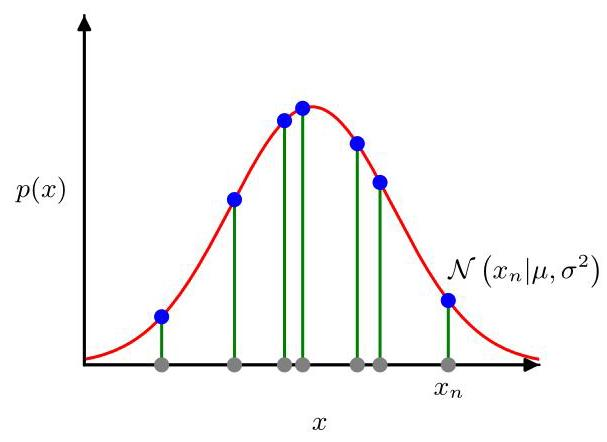
\includegraphics[max width=0.4\textwidth]{images/0194e279-9b28-703a-88f4-c3ac21e2010d_57_941_344_607_442_0.jpg}
\end{center}
\hspace*{3em} 

图 2.9 红色曲线展示了高斯分布的似然函数。这里灰色点表示值为 \(\left\{  {x}_{n}\right\}\) 的数据集,似然函数 (2.55) 由蓝色点表示的 \(p\left( x\right)\) 的对应值的乘积给出。最大化似然涉及调整高斯分布的均值和方差,以使这个乘积最大化。

当将其视为 \(\mu\) 和 \({\sigma }^{2}\) 的函数时,这被称为高斯分布的似然函数,如图 2.9 所示进行图解解释。

一种使用观测数据集确定概率分布中参数的常见方法,称为最大似然法,是找到使似然函数最大化的参数值。这可能看起来是一个奇怪的准则,因为从我们前面关于概率论的讨论来看,最大化给定数据下参数的概率,而不是给定参数下数据的概率,似乎更自然。实际上,这两个准则是相关的。

\HRule

第 2.6.2 节

\HRule

然而,首先我们将通过最大化似然函数 (2.55) 来确定高斯分布中未知参数 \(\mu\) 和 \({\sigma }^{2}\) 的值。在实践中,最大化似然函数的对数更为方便。因为对数是其自变量的单调递增函数,所以最大化一个函数的 \(\log\) 等价于最大化该函数本身。取 \(\log\) 不仅简化了后续的数学分析,而且在数值计算上也有帮助,因为大量小概率的乘积很容易导致计算机数值精度下溢,而通过计算对数概率的和可以解决这个问题。由 (2.49) 和 (2.55),对数似然函数可以写成如下形式

\[
\ln p\left( {\mathbf{x} \mid  \mu ,{\sigma }^{2}}\right)  =  - \frac{1}{2{\sigma }^{2}}\mathop{\sum }\limits_{{n = 1}}^{N}{\left( {x}_{n} - \mu \right) }^{2} - \frac{N}{2}\ln {\sigma }^{2} - \frac{N}{2}\ln \left( {2\pi }\right) . \tag{2.56}
\]

关于 \(\mu\) 最大化 (2.56),我们得到由下式给出的最大似然解

\[
{\mu }_{\mathrm{{ML}}} = \frac{1}{N}\mathop{\sum }\limits_{{n = 1}}^{N}{x}_{n} \tag{2.57}
\]

这就是样本均值,即观测值 \(\left\{  {x}_{n}\right\}\) 的均值。类似地,关于 \({\sigma }^{2}\) 最大化 (2.56),我们得到方差的最大似然解,形式如下

\[
{\sigma }_{\mathrm{{ML}}}^{2} = \frac{1}{N}\mathop{\sum }\limits_{{n = 1}}^{N}{\left( {x}_{n} - {\mu }_{\mathrm{{ML}}}\right) }^{2}, \tag{2.58}
\]

\HRule

练习 2.15

\HRule

这是相对于样本均值 \({\mu }_{\mathrm{{ML}}}\) 测量的样本方差。注意,我们正在对 (2.56) 关于 \(\mu\) 和 \({\sigma }^{2}\) 进行联合最大化,但对于高斯分布, \(\mu\) 的解与 \({\sigma }^{2}\) 的解是分离的,因此我们可以先计算 (2.57),然后再用这个结果计算 (2.58)。

\section*{2.3.3 最大似然估计的偏差}

最大似然技术在深度学习中被广泛使用,并且是大多数机器学习算法的基础。然而,它有一些局限性,我们可以用单变量高斯分布来说明这些局限性。

我们首先注意到,最大似然解 \({\mu }_{\mathrm{{ML}}}\) 和 \({\sigma }_{\mathrm{{ML}}}^{2}\) 是数据集值 \({x}_{1},\ldots ,{x}_{N}\) 的函数。假设这些值中的每一个都是从一个真实参数为 \(\mu\) 和 \({\sigma }^{2}\) 的高斯分布中独立生成的。现在考虑 \({\mu }_{\mathrm{{ML}}}\) 和 \({\sigma }_{\mathrm{{ML}}}^{2}\) 关于这些数据集值的期望。很容易证明

\[
\mathbb{E}\left\lbrack  {\mu }_{\mathrm{{ML}}}\right\rbrack   = \mu  \tag{2.59}
\]

\[
\mathbb{E}\left\lbrack  {\sigma }_{\mathrm{{ML}}}^{2}\right\rbrack   = \left( \frac{N - 1}{N}\right) {\sigma }^{2}. \tag{2.60}
\]

\HRule

练习 2.16

\HRule

我们看到,当对给定大小的数据集求平均时,均值的最大似然解将等于真实均值。然而,方差的最大似然估计将低估真实方差,低估因子为 \(\left( {N - 1}\right) /N\) 。这是一种称为偏差的现象的例子,在这种现象中,随机量的估计值与真实值存在系统性差异。图 2.10 给出了这个结果背后的直观解释。

请注意,偏差的产生是因为方差是相对于均值的最大似然估计来测量的,而均值的最大似然估计本身是根据数据进行调整的。假设我们可以获得真实均值 \(\mu\) ,并使用它来通过以下方式确定方差

估计量

\[
{\widehat{\sigma }}^{2} = \frac{1}{N}\mathop{\sum }\limits_{{n = 1}}^{N}{\left( {x}_{n} - \mu \right) }^{2}. \tag{2.61}
\]

练习 2.17 然后我们发现

\[
\mathbb{E}\left\lbrack  {\widehat{\sigma }}^{2}\right\rbrack   = {\sigma }^{2} \tag{2.62}
\]

这是无偏的。当然,我们无法获取真实均值,只能获取观测到的数据值。由结果 (2.60) 可知,对于高斯分布,方差参数的以下估计是无偏的:

\[
{\widetilde{\sigma }}^{2} = \frac{N}{N - 1}{\sigma }_{\mathrm{{ML}}}^{2} = \frac{1}{N - 1}\mathop{\sum }\limits_{{n = 1}}^{N}{\left( {x}_{n} - {\mu }_{\mathrm{{ML}}}\right) }^{2}. \tag{2.63}
\]

然而,在诸如神经网络等复杂模型中校正最大似然估计的偏差并非易事。

\begin{center}
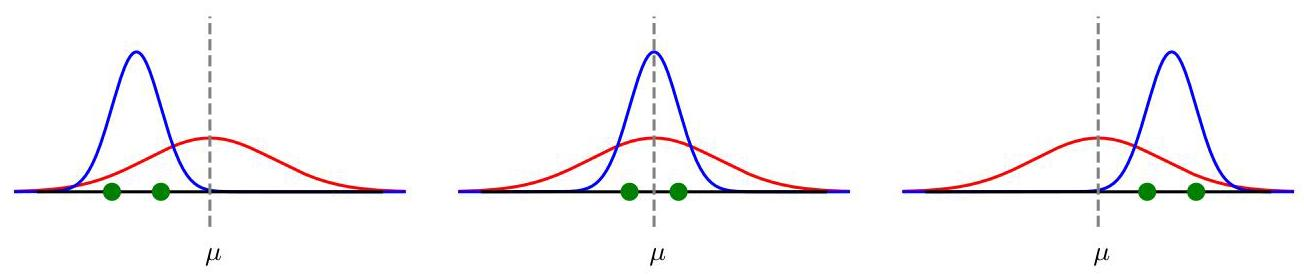
\includegraphics[max width=1.0\textwidth]{images/0194e279-9b28-703a-88f4-c3ac21e2010d_59_244_343_1304_276_0.jpg}
\end{center}
\hspace*{3em} 

图 2.10 展示了使用最大似然法确定高斯分布的均值和方差时偏差是如何产生的。红色曲线表示生成数据的真实高斯分布,三条蓝色曲线表示通过对三个数据集进行拟合得到的高斯分布,每个数据集由两个绿色显示的数据点组成,使用的是最大似然结果 (2.57) 和 (2.58)。对这三个数据集求平均后,均值是正确的,但方差被系统性地低估了,因为它是相对于样本均值而非真实均值来度量的。

请注意,随着数据点数量 \(N\) 的增加,最大似然解的偏差变得不那么显著。在极限情况 \(N \rightarrow  \infty\) 下,方差的最大似然解等于生成数据的分布的真实方差。对于高斯分布而言,除了数据点数量 \(N\) 较小时,这种偏差不会成为严重问题。然而,在本书中,我们将关注具有许多参数的复杂模型,对于这些模型,与最大似然估计相关的偏差问题会严重得多。实际上,最大似然估计中的偏差问题与过拟合问题密切相关。

\HRule

第 2.6.3 节

\HRule

\section*{2.3.4 线性回归}

我们已经了解了如何用误差最小化来表述线性回归问题。在这里,我们回到这个例子,从概率的角度来看待它,从而对误差函数和正则化有一些深入的理解。

\HRule

第1.2节

\HRule

回归问题的目标是,利用一组由 \(N\) 个输入值 \(\mathbf{x} = \left( {{x}_{1},\ldots ,{x}_{N}}\right)\) 及其对应的目标值 \(\mathbf{t} = \left( {{t}_{1},\ldots ,{t}_{N}}\right)\) 组成的训练数据,针对输入变量 \(x\) 的某个新值,对目标变量 \(t\) 进行预测。我们可以使用概率分布来表示对目标变量值的不确定性。为此,我们假设,给定 \(x\) 的值,对应的 \(t\) 的值服从高斯分布,其均值等于由(1.1)式给出的多项式曲线的值 \(y\left( {x,\mathbf{w}}\right)\) ,其中 \(\mathbf{w}\) 是多项式系数,方差为 \({\sigma }^{2}\) 。因此,我们有

\[
p\left( {t \mid  x,\mathbf{w},{\sigma }^{2}}\right)  = \mathcal{N}\left( {t \mid  y\left( {x,\mathbf{w}}\right) ,{\sigma }^{2}}\right) . \tag{2.64}
\]

这在图2.11中进行了示意性说明。

现在,我们使用训练数据 \(\{ \mathbf{x},\mathbf{t}\}\) 通过最大似然法来确定未知参数 \(\mathbf{w}\) 和 \({\sigma }^{2}\) 的值。如果假设数据是从……中抽取的

\begin{center}
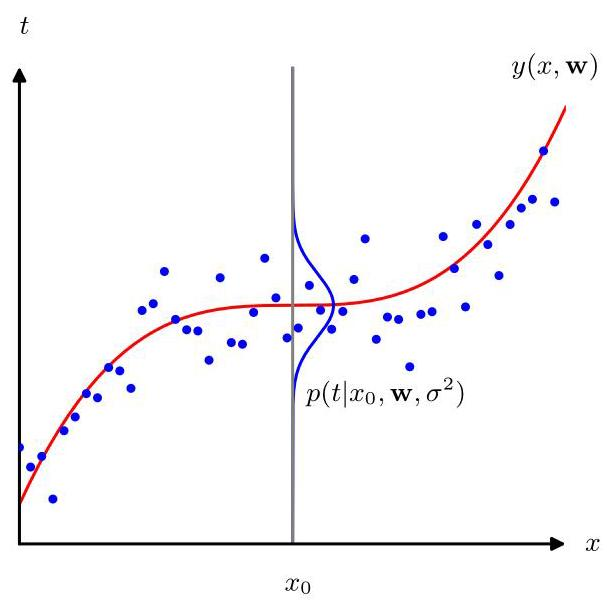
\includegraphics[max width=0.4\textwidth]{images/0194e279-9b28-703a-88f4-c3ac21e2010d_60_942_345_607_604_0.jpg}
\end{center}
\hspace*{3em} 

图 2.11 给定 \(x\) 时 \(t\) 的高斯条件分布的示意图,由式 (2.64) 定义,其中均值由多项式函数 \(y\left( {x,\mathbf{w}}\right)\) 给出,方差由参数 \({\sigma }^{2}\) 给出。

独立于分布 (2.64),则似然函数由下式给出

\[
p\left( {\mathbf{t} \mid  \mathbf{x},\mathbf{w},{\sigma }^{2}}\right)  = \mathop{\prod }\limits_{{n = 1}}^{N}\mathcal{N}\left( {{t}_{n} \mid  y\left( {{x}_{n},\mathbf{w}}\right) ,{\sigma }^{2}}\right) . \tag{2.65}
\]

正如我们之前对简单高斯分布所做的那样,最大化似然函数的对数是很方便的。将式 (2.49) 给出的高斯分布代入,我们得到如下形式的对数似然函数

\[
\ln p\left( {\mathbf{t} \mid  \mathbf{x},\mathbf{w},{\sigma }^{2}}\right)  =  - \frac{1}{2{\sigma }^{2}}\mathop{\sum }\limits_{{n = 1}}^{N}{\left\{  y\left( {x}_{n},\mathbf{w}\right)  - {t}_{n}\right\}  }^{2} - \frac{N}{2}\ln {\sigma }^{2} - \frac{N}{2}\ln \left( {2\pi }\right) . \tag{2.66}
\]

首先考虑对多项式系数的最大似然解进行评估,用 \({\mathbf{w}}_{\mathrm{{ML}}}\) 表示。这些系数是通过相对于 \(\mathbf{w}\) 最大化式 (2.66) 来确定的。为此,我们可以省略式 (2.66) 右侧的最后两项,因为它们不依赖于 w。此外,请注意,用一个正的常数系数对对数似然进行缩放不会改变相对于 \(\mathbf{w}\) 的最大值位置,因此我们可以用 \(1/2\) 替换系数 \(1/2{\sigma }^{2}\) 。最后,我们可以等效地最小化负对数似然而不是最大化对数似然。因此,就确定 \(\mathbf{w}\) 而言,我们看到最大化似然等效于最小化由下式定义的平方和误差函数

\[
E\left( \mathbf{w}\right)  = \frac{1}{2}\mathop{\sum }\limits_{{n = 1}}^{N}{\left\{  y\left( {x}_{n},\mathbf{w}\right)  - {t}_{n}\right\}  }^{2}. \tag{2.67}
\]

因此,平方和误差函数是在高斯噪声分布假设下最大化似然的结果。

我们还可以使用最大似然法来确定方差参数 \({\sigma }^{2}\) 。相对于 \({\sigma }^{2}\) 最大化式 (2.66) 可得

\[
{\sigma }_{\mathrm{{ML}}}^{2} = \frac{1}{N}\mathop{\sum }\limits_{{n = 1}}^{N}{\left\{  y\left( {x}_{n},{\mathbf{w}}_{\mathrm{{ML}}}\right)  - {t}_{n}\right\}  }^{2}. \tag{2.68}
\]

\HRule

练习 2.18

\HRule

注意,我们可以先确定控制均值的参数向量 \({\mathbf{w}}_{\mathrm{{ML}}}\) ,然后像简单高斯分布那样,用它来求方差 \({\sigma }_{\mathrm{{ML}}}^{2}\) 。

确定了参数 \(\mathbf{w}\) 和 \({\sigma }^{2}\) 之后,我们现在可以对 \(x\) 的新值进行预测。由于我们现在有了一个概率模型,这些预测用预测分布来表示,该分布给出了 \(t\) 上的概率分布,而不仅仅是一个点估计。通过将最大似然参数代入 (2.64) 式得到

\[
p\left( {t \mid  x,{\mathbf{w}}_{\mathrm{{ML}}},{\sigma }_{\mathrm{{ML}}}^{2}}\right)  = \mathcal{N}\left( {t \mid  y\left( {x,{\mathbf{w}}_{\mathrm{{ML}}}}\right) ,{\sigma }_{\mathrm{{ML}}}^{2}}\right) . \tag{2.69}
\]

\section*{2.4. 密度的变换}

现在我们来讨论概率密度在变量的非线性变换下是如何变化的。当我们讨论一类称为归一化流的生成模型时,这个性质将起到关键作用。它还凸显了在这种变换下,概率密度的行为与简单函数不同。

\HRule

第 18 章

\HRule

考虑一个单变量 \(x\) ,并假设我们进行变量变换 \(x =\)  \(g\left( y\right)\) ,那么一个函数 \(f\left( x\right)\) 就变成了一个由下式定义的新函数 \(\widetilde{f}\left( y\right)\)

\[
\widetilde{f}\left( y\right)  = f\left( {g\left( y\right) }\right) . \tag{2.70}
\]

现在考虑一个概率密度 \({p}_{x}\left( x\right)\) ,再次使用 \(x =\)  \(g\left( y\right)\) 进行变量变换,得到一个关于新变量 \(y\) 的密度 \({p}_{y}\left( y\right)\) ,其中下标表示 \({p}_{x}\left( x\right)\) 和 \({p}_{y}\left( y\right)\) 是不同的密度。对于小的 \({\delta x}\) 值,落在区间 \(\left( {x,x + {\delta x}}\right)\) 内的观测值将被变换到区间 \(\left( {y,y + {\delta y}}\right)\) 内,其中 \(x = g\left( y\right)\) ,且 \({p}_{x}\left( x\right) {\delta x} \simeq  {p}_{y}\left( y\right) {\delta y}\) 。因此,如果我们取极限 \({\delta x} \rightarrow  0\) ,我们得到

\[
{p}_{y}\left( y\right)  = {p}_{x}\left( x\right) \left| \frac{\mathrm{d}x}{\mathrm{\;d}y}\right|
\]

\[
= {p}_{x}\left( {g\left( y\right) }\right) \left| \frac{\mathrm{d}g}{\mathrm{\;d}y}\right| . \tag{2.71}
\]

这里的模 \(\left| \cdot \right|\) 出现是因为导数 \(\mathrm{d}y/\mathrm{d}x\) 可能为负,而密度是按长度比进行缩放的,长度比总是正的。

这种变换密度的方法可能非常强大。任何密度 \(p\left( y\right)\) 都可以通过对一个处处非零的固定密度 \(q\left( x\right)\) 进行非线性变量变换 \(y = f\left( x\right)\) 得到,其中 \(f\left( x\right)\) 是一个单调函数,使得 \(0 \leq  {f}^{\prime }\left( x\right)  < \infty\) 。

\HRule

练习 2.19

\HRule

变换性质 (2.71) 的一个结果是,概率密度最大值的概念依赖于变量的选择。假设 \(f\left( x\right)\) 在 \(\widehat{x}\) 处有一个众数(即最大值),使得 \({f}^{\prime }\left( \widehat{x}\right)  = 0\) 。 \(\widetilde{f}\left( y\right)\) 的相应众数将出现在通过对 (2.70) 两边关于 \(y\) 求导得到的值 \(\widehat{y}\) 处:

\[
{\widetilde{f}}^{\prime }\left( \widehat{y}\right)  = {f}^{\prime }\left( {g\left( \widehat{y}\right) }\right) {g}^{\prime }\left( \widehat{y}\right)  = 0. \tag{2.72}
\]

假设在众数处有 \({g}^{\prime }\left( \widehat{y}\right)  \neq  0\) ,那么 \({f}^{\prime }\left( {g\left( \widehat{y}\right) }\right)  = 0\) 。然而,我们知道 \({f}^{\prime }\left( \widehat{x}\right)  = 0\) ,因此可以看到,用变量 \(x\) 和 \(y\) 表示的众数位置由 \(\widehat{x} = g\left( \widehat{y}\right)\) 相关联,这是符合预期的。因此,找到关于变量 \(x\) 的众数等价于先转换到变量 \(y\) ,然后找到关于 \(y\) 的众数,再转换回 \(x\) 。

现在考虑概率密度 \({p}_{x}\left( x\right)\) 在变量变换 \(x = g\left( y\right)\) 下的行为,其中关于新变量的密度为 \({p}_{y}\left( y\right)\) ,由式 (2.71) 给出。为了处理式 (2.71) 中的模,我们可以写成 \({g}^{\prime }\left( y\right)  = s\left| {{g}^{\prime }\left( y\right) }\right|\) ,其中 \(s \in  \{  - 1, + 1\}\) 。那么式 (2.71) 可以写成

\[
{p}_{y}\left( y\right)  = {p}_{x}\left( {g\left( y\right) }\right) s{g}^{\prime }\left( y\right)
\]

这里我们使用了 \(1/s = s\) 。然后对两边关于 \(y\) 求导可得

\[
{p}_{y}^{\prime }\left( y\right)  = s{p}_{x}^{\prime }\left( {g\left( y\right) }\right) {\left\{  {g}^{\prime }\left( y\right) \right\}  }^{2} + s{p}_{x}\left( {g\left( y\right) }\right) {g}^{\prime \prime }\left( y\right) . \tag{2.73}
\]

由于式 (2.73) 右侧第二项的存在,关系 \(\widehat{x} = g\left( \widehat{y}\right)\) 不再成立。因此,通过最大化 \({p}_{x}\left( x\right)\) 得到的 \(x\) 值将不是先转换到 \({p}_{y}\left( y\right)\) ,然后关于 \(y\) 最大化,再转换回 \(x\) 所得到的值。这导致密度的众数依赖于变量的选择。然而,对于线性变换,式 (2.73) 右侧的第二项消失,因此在这种情况下,最大值的位置根据 \(\widehat{x} = g\left( \widehat{y}\right)\) 进行变换。

如图 2.12 所示,这个效应可以用一个简单的例子来说明。我们首先考虑在 \(x\) 上的高斯分布 \({p}_{x}\left( x\right)\) ,如图 2.12 中的红色曲线所示。接下来,我们从这个分布中抽取 \(N = {50},{000}\) 个点的样本,并绘制它们值的直方图,正如预期的那样,该直方图与分布 \({p}_{x}\left( x\right)\) 一致。现在考虑从 \(x\) 到 \(y\) 的非线性变量变换,由下式给出

\[
x = g\left( y\right)  = \ln \left( y\right)  - \ln \left( {1 - y}\right)  + 5. \tag{2.74}
\]

这个函数的反函数由下式给出

\[
y = {g}^{-1}\left( x\right)  = \frac{1}{1 + \exp \left( {-x + 5}\right) }, \tag{2.75}
\]

这是一个逻辑 sigmoid 函数,在图 2.12 中用蓝色曲线表示。

\begin{center}
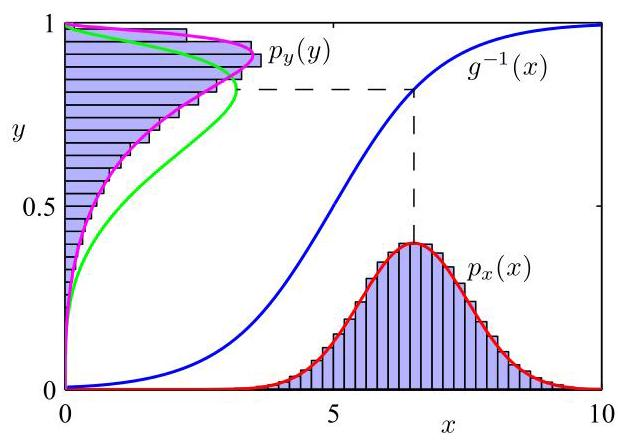
\includegraphics[max width=0.5\textwidth]{images/0194e279-9b28-703a-88f4-c3ac21e2010d_63_930_349_618_442_0.jpg}
\end{center}
\hspace*{3em} 

图 2.12 展示了在变量进行非线性变换时,密度模式的转换示例,说明了与简单函数相比的不同行为。

如果我们简单地将 \({p}_{x}\left( x\right)\) 作为 \(x\) 的函数进行变换,我们会得到图 2.12 中所示的绿色曲线 \({p}_{x}\left( {g\left( y\right) }\right)\) ,并且我们看到密度 \({p}_{x}\left( x\right)\) 的模式通过 sigmoid 函数变换为该曲线的模式。然而, \(y\) 上的密度则根据 (2.71) 进行变换,并在图的左侧用洋红色曲线表示。请注意,其模式相对于绿色曲线的模式发生了偏移。

为了证实这一结果,我们选取 50,000 个 \(x\) 的值作为样本,使用 (2.75) 计算相应的 \(y\) 的值,然后绘制它们值的直方图。我们发现这个直方图与图 2.12 中的洋红色曲线相符,而不是绿色曲线。

\section*{2.4.1 多元分布}

我们可以将结果 (2.71) 扩展到定义在多个变量上的密度。考虑一个关于 \(D\) 维变量 \(\mathbf{x} = {\left( {x}_{1},\ldots ,{x}_{D}\right) }^{\mathrm{T}}\) 的密度 \(p\left( \mathbf{x}\right)\) ,并假设我们变换到一个新变量 \(\mathbf{y} = {\left( {y}_{1},\ldots ,{y}_{D}\right) }^{\mathrm{T}}\) ,其中 \(\mathbf{x} = \mathbf{g}\left( \mathbf{y}\right)\) 。在这里,我们将自己限制在 \(\mathbf{x}\) 和 \(\mathbf{y}\) 具有相同维度的情况。然后,变换后的密度由 (2.71) 的推广形式给出

\[
{p}_{\mathbf{y}}\left( \mathbf{y}\right)  = {p}_{\mathbf{x}}\left( \mathbf{x}\right) \left| {\det \mathbf{J}}\right|  \tag{2.76}
\]

其中 \(\mathbf{J}\) 是雅可比矩阵,其元素由偏导数 \({J}_{ij} = \partial {g}_{i}/\partial {y}_{j}\) 给出,因此

\[
\mathbf{J} = \left\lbrack  \begin{matrix} \frac{\partial {g}_{1}}{\partial {y}_{1}} & \cdots & \frac{\partial {g}_{1}}{\partial {y}_{D}} \\  \vdots &  \ddots  & \vdots \\  \frac{\partial {g}_{D}}{\partial {y}_{1}} & \cdots & \frac{\partial {g}_{D}}{\partial {y}_{D}} \end{matrix}\right\rbrack  . \tag{2.77}
\]

直观地说,我们可以将变量变换视为对空间的某些区域进行扩展,而对其他区域进行收缩,围绕点 \(\mathrm{x}\) 的无穷小区域 \(\Delta \mathrm{x}\) 被变换为围绕点 \(\mathbf{y} = \mathbf{g}\left( \mathbf{x}\right)\) 的区域 \(\Delta \mathbf{y}\) 。雅可比行列式的绝对值表示这些体积的比率,并且与在积分中进行变量变换时出现的因子相同。公式 (2.77) 源于区域 \(\Delta \mathrm{x}\) 中的概率质量与 \(\Delta \mathbf{y}\) 中的概率质量相同这一事实。我们再次取模以确保密度是非负的。

\begin{center}
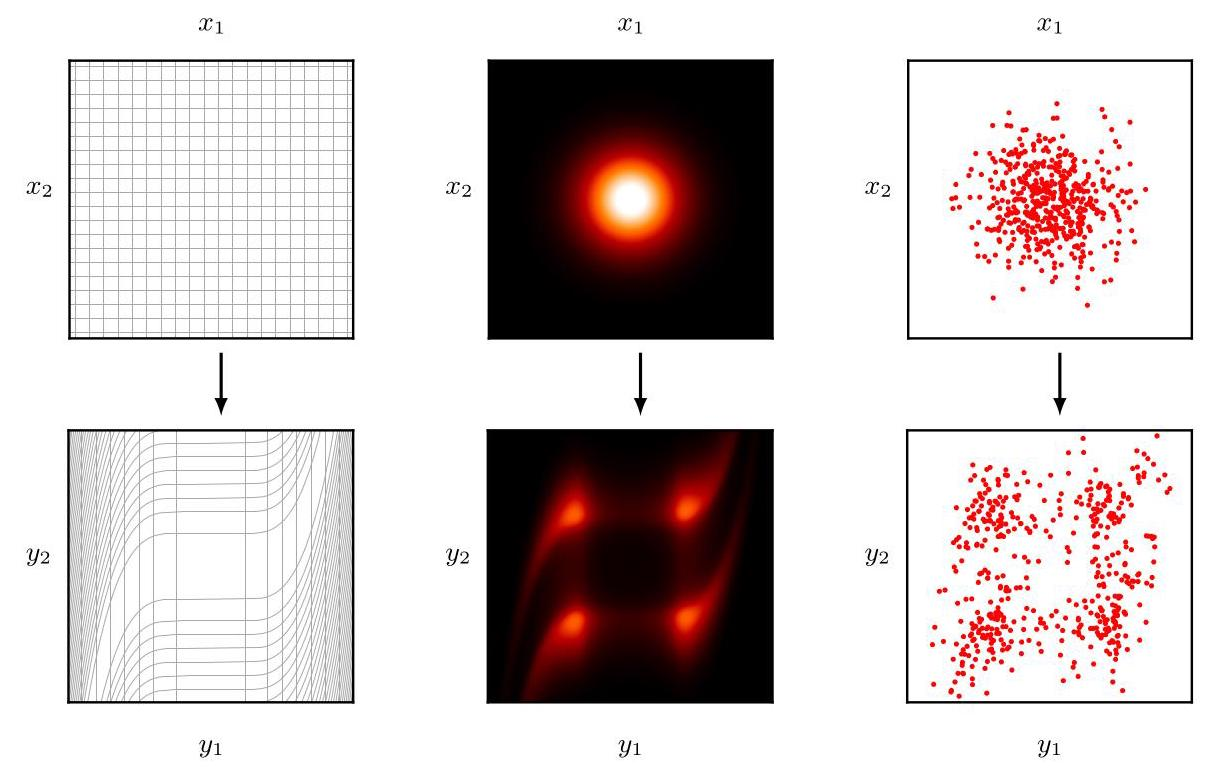
\includegraphics[max width=0.9\textwidth]{images/0194e279-9b28-703a-88f4-c3ac21e2010d_64_290_359_1210_772_0.jpg}
\end{center}
\hspace*{3em} 

图 2.13 展示了二维概率分布中变量变换的效果。左列显示了变量的变换,而中间列和右列分别显示了对高斯分布及其样本的相应影响。

我们可以通过对二维高斯分布应用变量变换来说明这一点,如图 2.13 顶行所示。这里的变换

练习 2.20 从 \(\mathbf{x}\) 到 \(\mathbf{y}\) 的变换由下式给出

\[
{y}_{1} = {x}_{1} + \tanh \left( {5{x}_{1}}\right)  \tag{2.78}
\]

\[
{y}_{2} = {x}_{2} + \tanh \left( {5{x}_{2}}\right)  + \frac{{x}_{1}^{3}}{3}. \tag{2.79}
\]

底行还展示了 \(\mathbf{x}\) 空间中高斯分布的样本以及 \(\mathbf{y}\) 空间中相应的变换样本。

\section*{2.5. 信息论}

概率论构成了另一个重要框架——信息论的基础。信息论对数据集中存在的信息进行量化,并且在机器学习中发挥着重要作用。在这里,我们简要介绍信息论的一些关键要素,这些要素在本书后面的内容中会用到,包括各种形式的重要概念——熵。关于信息论与机器学习的联系的更全面介绍,请参阅 MacKay (2003)。

\section*{2.5.1 熵}

我们首先考虑一个离散随机变量 \(x\) ,并询问当我们观察到该变量的一个特定值时,我们接收到了多少信息。信息的数量可以看作是得知 \(x\) 的值时的“惊讶程度”。如果我们被告知一个极不可能发生的事件刚刚发生,那么我们接收到的信息比被告知一个非常可能发生的事件刚刚发生时要多;如果我们知道某个事件肯定会发生,那么我们就不会接收到任何信息。因此,我们对信息内容的度量将取决于概率分布 \(p\left( x\right)\) ,所以我们要寻找一个量 \(h\left( x\right)\) ,它是概率 \(p\left( x\right)\) 的单调函数,并能表达信息内容。通过注意到如果我们有两个不相关的事件 \(x\) 和 \(y\) ,那么观察到这两个事件所获得的信息应该是分别观察每个事件所获得的信息之和,即 \(h\left( {x,y}\right)  = h\left( x\right)  + h\left( y\right)\) 。两个不相关的事件在统计上是独立的,所以 \(p\left( {x,y}\right)  = p\left( x\right) p\left( y\right)\) 。从这两个关系中,很容易证明 \(h\left( x\right)\) 必须由 \(p\left( x\right)\) 的对数给出,因此我们有

\[
h\left( x\right)  =  - {\log }_{2}p\left( x\right)  \tag{2.80}
\]

\HRule

练习 2.21

\HRule

其中负号确保信息为正或零。请注意,低概率事件 \(x\) 对应着高信息内容。对数的底数选择是任意的,目前我们将采用信息论中普遍使用的以 2 为底的对数约定。在这种情况下,正如我们很快会看到的, \(h\left( x\right)\) 的单位是比特(“二进制数字”)。

现在假设发送方希望将一个随机变量的值传输给接收方。他们在此过程中传输的平均信息量是通过对 (2.80) 关于分布 \(p\left( x\right)\) 取期望得到的,其表达式为

\[
\mathrm{H}\left\lbrack  x\right\rbrack   =  - \mathop{\sum }\limits_{x}p\left( x\right) {\log }_{2}p\left( x\right) . \tag{2.81}
\]

这个重要的量被称为随机变量 \(x\) 的熵。注意到 \(\mathop{\lim }\limits_{{\epsilon  \rightarrow  0}}\left( {\epsilon \ln \epsilon }\right)  = 0\) ,因此每当我们遇到 \(x\) 的值使得 \(p\left( x\right)  = 0\) 时,我们将取 \(p\left( x\right) \ln p\left( x\right)  = 0\) 。

到目前为止,我们对信息的定义 (2.80) 以及相应的熵的定义 (2.81) 给出了一种较为启发式的动机。现在我们证明这些定义确实具有有用的性质。考虑一个具有八个可能状态的随机变量 \(x\) ,每个状态的可能性相等。为了将 \(x\) 的值传达给接收方,我们需要传输一个长度为 3 比特的消息。注意到这个变量的熵为

\[
\mathrm{H}\left\lbrack  x\right\rbrack   =  - 8 \times  \frac{1}{8}{\log }_{2}\frac{1}{8} = 3\text{ bits. }
\]

现在考虑一个例子(Cover 和 Thomas,1991),一个变量具有八个可能的状态 \(\{ a,b,c,d,e,f,g,h\}\) ,其各自的概率由 \(\left( {\frac{1}{2},\frac{1}{4},\frac{1}{8},\frac{1}{16},\frac{1}{64},\frac{1}{64},\frac{1}{64},\frac{1}{64}}\right)\) 给出。在这种情况下,熵为

\[
\mathrm{H}\left\lbrack  x\right\rbrack   =  - \frac{1}{2}{\log }_{2}\frac{1}{2} - \frac{1}{4}{\log }_{2}\frac{1}{4} - \frac{1}{8}{\log }_{2}\frac{1}{8} - \frac{1}{16}{\log }_{2}\frac{1}{16} - \frac{4}{64}{\log }_{2}\frac{1}{64} = 2\text{ bits. }
\]

我们看到,非均匀分布的熵比均匀分布的熵小。当我们从无序性的角度讨论熵的解释时,很快就会对这一点有更深入的理解。目前,让我们考虑如何将变量的状态标识传输给接收方。和之前一样,我们可以使用一个 3 比特的数字来完成。然而,我们可以利用非均匀分布的特点,为更可能发生的事件使用更短的编码,而为不太可能发生的事件使用更长的编码,以期获得更短的平均编码长度。例如,可以使用以下一组编码字符串来表示状态 \(\{ a,b,c,d,e,f,g,h\}\) :0、10、110、1110、111100、111101、111110 和 111111。那么需要传输的编码的平均长度为

平均编码长度 \(= \frac{1}{2} \times  1 + \frac{1}{4} \times  2 + \frac{1}{8} \times  3 + \frac{1}{16} \times  4 + 4 \times  \frac{1}{64} \times  6 = 2\) 比特

这再次与随机变量的熵相同。请注意,不能使用更短的代码字符串,因为必须能够将这样的字符串的串联明确地拆分为其组成部分。例如,11001110 能唯一地解码为状态序列 \(c,a,d\) 。熵与最短编码长度之间的这种关系是一种普遍关系。无噪声编码定理(Shannon,1948)指出,熵是传输随机变量状态所需比特数的下限。

从现在起,我们将在定义熵时改用自然对数,因为这将与本书其他地方的概念建立更便捷的联系。在这种情况下,熵的单位是奈特(来自“自然对数”)而非比特,二者仅相差一个因子 \(\ln 2\) 。

\section*{2.5.2 物理学视角}

我们从指定随机变量状态所需的平均信息量的角度引入了熵的概念。实际上,熵的概念在物理学中的起源要早得多,它最初是在平衡热力学的背景下引入的,后来通过统计力学的发展被赋予了更深刻的解释,即作为无序程度的度量。我们可以通过考虑一组 \(N\) 个相同的物体来理解熵的这种另类观点,这些物体要被分配到一组箱子中,使得第 \(i\) 个箱子中有 \({n}_{i}\) 个物体。考虑将物体分配到箱子中的不同方式的数量。选择第一个物体有 \(N\) 种方法,选择第二个物体有 \(\left( {N - 1}\right)\) 种方法,依此类推,将所有 \(N\) 个物体分配到箱子中的总方法数为 \(N\) ! 种,其中 \(N\) !(读作“ \(N\) 的阶乘”)表示乘积 \(N \times  \left( {N - 1}\right)  \times  \cdots  \times  2 \times  1\) 。然而,我们不希望区分每个箱子内物体的重新排列。在第 \(i\) 个箱子中,有 \({n}_{i}\) ! 种重新排列物体的方法,因此将 \(N\) 个物体分配到箱子中的总方法数为

\[
W = \frac{N!}{\mathop{\prod }\limits_{i}{n}_{i}!}, \tag{2.82}
\]

这被称为多重性。然后,熵被定义为多重性的对数乘以一个常数因子 \(1/N\) ,即

\[
\mathrm{H} = \frac{1}{N}\ln W = \frac{1}{N}\ln N! - \frac{1}{N}\mathop{\sum }\limits_{i}\ln {n}_{i}!. \tag{2.83}
\]

现在我们考虑极限 \(N \rightarrow  \infty\) ,其中分数 \({n}_{i}/N\) 保持不变,并应用斯特林近似:

\[
\ln N! \simeq  N\ln N - N \tag{2.84}
\]

由此可得

\[
\mathrm{H} =  - \mathop{\lim }\limits_{{N \rightarrow  \infty }}\mathop{\sum }\limits_{i}\left( \frac{{n}_{i}}{N}\right) \ln \left( \frac{{n}_{i}}{N}\right)  =  - \mathop{\sum }\limits_{i}{p}_{i}\ln {p}_{i} \tag{2.85}
\]

其中我们使用了 \(\mathop{\sum }\limits_{i}{n}_{i} = N\) 。这里 \({p}_{i} = \mathop{\lim }\limits_{{N \rightarrow  \infty }}\left( {{n}_{i}/N}\right)\) 是一个对象被分配到第 \(i\) 个容器的概率。用物理学的术语来说,将对象具体分配到各个容器的方式称为微观态,而通过比率 \({n}_{i}/N\) 表示的占据数的总体分布称为宏观态。表示给定宏观态中微观态数量的多重性 \(W\) ,也被称为该宏观态的权重。

我们可以将这些容器解释为离散随机变量 \(X\) 的状态 \({x}_{i}\) ,其中 \(p\left( {X = {x}_{i}}\right)  = {p}_{i}\) 。那么随机变量 \(X\) 的熵为

\[
\mathrm{H}\left\lbrack  p\right\rbrack   =  - \mathop{\sum }\limits_{i}p\left( {x}_{i}\right) \ln p\left( {x}_{i}\right) . \tag{2.86}
\]

如图 2.14 所示,在少数几个值附近有尖锐峰值的分布 \(p\left( {x}_{i}\right)\) 的熵相对较低,而那些更均匀地分布在多个值上的分布的熵则较高。

因为 \(0 \leq  {p}_{i} \leq  1\) ,所以熵是非负的,并且当其中一个 \({p}_{i} = 1\) 且所有其他 \({p}_{j \neq  i} = 0\) 时,熵将等于其最小值 0。可以通过使用拉格朗日乘数法来最大化 \(\mathrm{H}\) 并同时满足概率的归一化约束条件,从而找到最大熵配置。因此,我们最大化

\[
\widetilde{\mathrm{H}} =  - \mathop{\sum }\limits_{i}p\left( {x}_{i}\right) \ln p\left( {x}_{i}\right)  + \lambda \left( {\mathop{\sum }\limits_{i}p\left( {x}_{i}\right)  - 1}\right)  \tag{2.87}
\]

由此我们发现所有的 \(p\left( {x}_{i}\right)\) 都相等,且由 \(p\left( {x}_{i}\right)  = 1/M\) 给出,其中 \(M\) 是状态 \({x}_{i}\) 的总数。那么熵的相应值为 \(\mathrm{H} = \ln M\) 。这个结果也可以从 Jensen 不等式(稍后讨论)推导得出。为了验证该驻点确实是最大值,我们可以计算熵的二阶导数,结果为

\[
\frac{\partial \widetilde{\mathrm{H}}}{\partial p\left( {x}_{i}\right) \partial p\left( {x}_{j}\right) } =  - {I}_{ij}\frac{1}{{p}_{i}} \tag{2.88}
\]

\HRule

附录 \(C\)

\HRule

\begin{center}
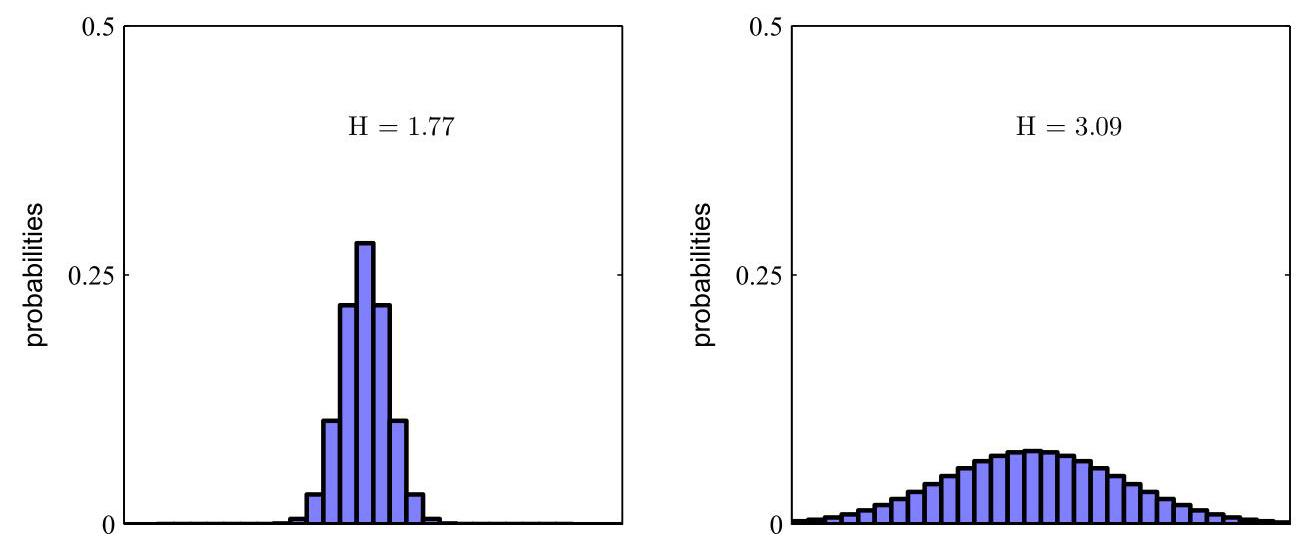
\includegraphics[max width=1.0\textwidth]{images/0194e279-9b28-703a-88f4-c3ac21e2010d_68_224_402_1306_548_0.jpg}
\end{center}
\hspace*{3em} 

图 2.14 两个概率分布在 30 个区间上的直方图,展示了更宽泛分布的熵 \(\mathrm{H}\) 值更高。最大熵将来自均匀分布,其值为 \(\mathrm{H} =  - \ln \left( {1/{30}}\right)  = {3.40}\) 。

\HRule

练习 2.22

练习 2.23

\HRule

其中 \({I}_{ij}\) 是单位矩阵的元素。我们看到这些值都是负的,因此,该驻点确实是一个最大值点。

\section*{2.5.3 微分熵}

我们可以将熵的定义扩展到包含连续变量 \(x\) 上的分布 \(p\left( x\right)\) ,具体如下。首先,将 \(x\) 划分为宽度为 \(\Delta\) 的区间。然后,假设 \(p\left( x\right)\) 是连续的,中值定理(Weisstein,1999)告诉我们,对于每个这样的区间,在范围 \({i\Delta } \leq  {x}_{i} \leq  \left( {i + 1}\right) \Delta\) 内必定存在一个值 \({x}_{i}\) ,使得

\[
{\int }_{i\Delta }^{\left( {i + 1}\right) \Delta }p\left( x\right) \mathrm{d}x = p\left( {x}_{i}\right) \Delta . \tag{2.89}
\]

现在,我们可以对连续变量 \(x\) 进行量化,每当 \(x\) 落在第 \(i\) 个区间时,就将其赋值为 \({x}_{i}\) 。那么,观测到值 \({x}_{i}\) 的概率就是 \(p\left( {x}_{i}\right) \Delta\) 。这就得到了一个离散分布,其熵的形式为

\[
{\mathrm{H}}_{\Delta } =  - \mathop{\sum }\limits_{i}p\left( {x}_{i}\right) \Delta \ln \left( {p\left( {x}_{i}\right) \Delta }\right)  =  - \mathop{\sum }\limits_{i}p\left( {x}_{i}\right) \Delta \ln p\left( {x}_{i}\right)  - \ln \Delta  \tag{2.90}
\]

这里我们使用了 \(\mathop{\sum }\limits_{i}p\left( {x}_{i}\right) \Delta  = 1\) ,它由式(2.89)和式(2.25)得出。现在,我们忽略式(2.90)右侧的第二项 \(- \ln \Delta\) ,因为它与 \(p\left( x\right)\) 无关,然后考虑极限 \(\Delta  \rightarrow  0\) 。在这个极限下,式(2.90)右侧的第一项将趋近于 \(p\left( x\right) \ln p\left( x\right)\) 的积分,使得

\[
\mathop{\lim }\limits_{{\Delta  \rightarrow  0}}\left\{  {-\mathop{\sum }\limits_{i}p\left( {x}_{i}\right) \Delta \ln p\left( {x}_{i}\right) }\right\}   =  - \int p\left( x\right) \ln p\left( x\right) \mathrm{d}x \tag{2.91}
\]

其中,右侧的量被称为微分熵。我们看到,熵的离散形式和连续形式相差一个量 \(\ln \Delta\) ,该量在极限 \(\Delta  \rightarrow  0\) 下趋于无穷。这反映出,要非常精确地指定一个连续变量需要大量的比特。对于定义在多个连续变量上的概率密度(用向量 \(\mathrm{x}\) 统一表示),微分熵由下式给出

\[
\mathrm{H}\left\lbrack  \mathbf{x}\right\rbrack   =  - \int p\left( \mathbf{x}\right) \ln p\left( \mathbf{x}\right) \mathrm{d}\mathbf{x}. \tag{2.92}
\]

\section*{2.5.4 最大熵}

我们已经知道,对于离散分布,最大熵配置对应于变量所有可能状态上的均匀概率分布。现在,让我们考虑连续变量的相应结果。为了使这个最大值有明确定义,有必要对 \(p\left( x\right)\) 的一阶矩和二阶矩进行约束,并保留归一化约束。因此,我们在以下三个约束条件下最大化微分熵:

\[
{\int }_{-\infty }^{\infty }p\left( x\right) \mathrm{d}x = 1 \tag{2.93}
\]

\[
{\int }_{-\infty }^{\infty }{xp}\left( x\right) \mathrm{d}x = \mu  \tag{2.94}
\]

\[
{\int }_{-\infty }^{\infty }{\left( x - \mu \right) }^{2}p\left( x\right) \mathrm{d}x = {\sigma }^{2}. \tag{2.95}
\]

\HRule

附录 \(C\)

\HRule

可以使用拉格朗日乘数法进行约束最大化,从而使我们关于 \(p\left( x\right)\) 最大化以下泛函:

\[
- {\int }_{-\infty }^{\infty }p\left( x\right) \ln p\left( x\right) \mathrm{d}x + {\lambda }_{1}\left( {{\int }_{-\infty }^{\infty }p\left( x\right) \mathrm{d}x - 1}\right)
\]

\[
+ {\lambda }_{2}\left( {{\int }_{-\infty }^{\infty }{xp}\left( x\right) \mathrm{d}x - \mu }\right)  + {\lambda }_{3}\left( {{\int }_{-\infty }^{\infty }{\left( x - \mu \right) }^{2}p\left( x\right) \mathrm{d}x - {\sigma }^{2}}\right) . \tag{2.96}
\]

使用变分法,我们将该泛函的导数设为零,得到

\[
p\left( x\right)  = \exp \left\{  {-1 + {\lambda }_{1} + {\lambda }_{2}x + {\lambda }_{3}{\left( x - \mu \right) }^{2}}\right\}  . \tag{2.97}
\]

\HRule

附录 B

\HRule

通过将此结果回代到三个约束方程中,可以求出拉格朗日乘数,最终得到结果:

\[
p\left( x\right)  = \frac{1}{{\left( 2\pi {\sigma }^{2}\right) }^{1/2}}\exp \left\{  {-\frac{{\left( x - \mu \right) }^{2}}{2{\sigma }^{2}}}\right\}  , \tag{2.98}
\]

\HRule

练习 2.24

\HRule

因此,使微分熵最大化的分布是高斯分布。请注意,在最大化熵时,我们并未对分布进行非负约束。然而,由于得到的分布实际上是非负的,事后看来,这样的约束并非必要。

\HRule

练习 2.25

\HRule

如果我们计算高斯分布的微分熵,我们会得到

\[
\mathrm{H}\left\lbrack  x\right\rbrack   = \frac{1}{2}\left\{  {1 + \ln \left( {{2\pi }{\sigma }^{2}}\right) }\right\}  . \tag{2.99}
\]

因此,我们再次看到,随着分布变宽,即随着 \({\sigma }^{2}\) 增大,熵也会增加。这个结果还表明,与离散熵不同,微分熵可以为负,因为对于 \({\sigma }^{2} < 1/\left( {2\pi e}\right)\) ,(2.99) 式中的 \(\mathrm{H}\left( x\right)  < 0\) 。

\section*{2.5.5 库尔贝克 - 莱布勒散度}

到目前为止,在本节中,我们已经介绍了信息论中的一些概念,包括熵这一关键概念。现在我们开始将这些概念与机器学习联系起来。考虑某个未知分布 \(p\left( \mathbf{x}\right)\) ,并假设我们使用一个近似分布 \(q\left( \mathbf{x}\right)\) 对其进行建模。如果我们使用 \(q\left( \mathbf{x}\right)\) 来构建一个编码方案,用于向接收方传输 \(\mathbf{x}\) 的值,那么由于使用 \(q\left( \mathbf{x}\right)\) 而非真实分布 \(p\left( \mathbf{x}\right)\) 来指定 \(\mathbf{x}\) 的值(假设我们选择了一个高效的编码方案)所需的平均额外信息量(以奈特为单位)由下式给出

\[
\operatorname{KL}\left( {p\parallel q}\right)  =  - \int p\left( \mathbf{x}\right) \ln q\left( \mathbf{x}\right) \mathrm{d}\mathbf{x} - \left( {-\int p\left( \mathbf{x}\right) \ln p\left( \mathbf{x}\right) \mathrm{d}\mathbf{x}}\right)
\]

\[
=  - \int p\left( \mathbf{x}\right) \ln \left\{  \frac{q\left( \mathbf{x}\right) }{p\left( \mathbf{x}\right) }\right\}  \mathrm{d}\mathbf{x}. \tag{2.100}
\]

这被称为分布 \(p\left( \mathbf{x}\right)\) 和 \(q\left( \mathbf{x}\right)\) 之间的相对熵或 Kullback-Leibler 散度,简称 KL 散度(Kullback 和 Leibler,1951)。需要注意的是,它不是一个对称量,也就是说 \(\mathrm{{KL}}\left( {p\parallel q}\right)  ≢ \mathrm{{KL}}\left( {q\parallel p}\right)\) 。

现在我们证明,当且仅当 \(p\left( \mathbf{x}\right)  = q\left( \mathbf{x}\right)\) 时,Kullback-Leibler 散度满足 \(\operatorname{KL}\left( {p\parallel q}\right)  \geq  0\) 且等号成立。为此,我们首先引入凸函数的概念。如果函数 \(f\left( x\right)\) 具有每条弦都位于函数之上或与函数重合的性质,则称该函数为凸函数,如图 2.15 所示。

区间 \(x = a\) 到 \(x = b\) 内的任意 \(x\) 值都可以写成 \({\lambda a} + \left( {1 - \lambda }\right) b\) 的形式,其中 \(0 \leq  \lambda  \leq  1\) 。弦上对应的点

\begin{center}
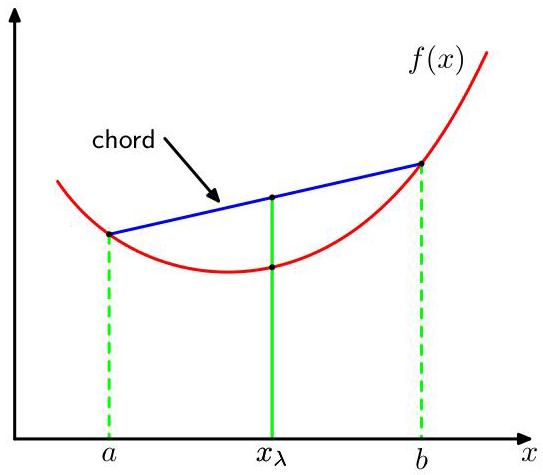
\includegraphics[max width=0.4\textwidth]{images/0194e279-9b28-703a-88f4-c3ac21e2010d_71_1002_349_543_475_0.jpg}
\end{center}
\hspace*{3em} 

图 2.15 凸函数 \(f\left( x\right)\) 的每条弦(蓝色所示)都位于函数(红色所示)之上或与函数重合。

由 \({\lambda f}\left( a\right)  + \left( {1 - \lambda }\right) f\left( b\right)\) 给出,函数的对应值为 \(f\left( {{\lambda a} + \left( {1 - \lambda }\right) b}\right)\) 。那么凸性意味着

\[
f\left( {{\lambda a} + \left( {1 - \lambda }\right) b}\right)  \leq  {\lambda f}\left( a\right)  + \left( {1 - \lambda }\right) f\left( b\right) . \tag{2.101}
\]

这等价于要求函数的二阶导数处处为正。凸函数的例子有 \(x\ln x\) (对于 \(x > 0\) )和 \({x}^{2}\) 。如果仅当 \(\lambda  = 0\) 和 \(\lambda  = 1\) 时等号成立,则称该函数为严格凸函数。如果一个函数具有相反的性质,即每条弦都位于函数之下或与函数重合,则称该函数为凹函数,严格凹函数也有相应的定义。如果函数 \(f\left( x\right)\) 是凸函数,那么 \(- f\left( x\right)\) 将是凹函数。

\HRule

练习 2.32

练习 2.33

\HRule

使用归纳证明的技巧,我们可以从 (2.101) 式证明凸函数 \(f\left( x\right)\) 满足

\[
f\left( {\mathop{\sum }\limits_{{i = 1}}^{M}{\lambda }_{i}{x}_{i}}\right)  \leq  \mathop{\sum }\limits_{{i = 1}}^{M}{\lambda }_{i}f\left( {x}_{i}\right)  \tag{2.102}
\]

其中 \({\lambda }_{i} \geq  0\) 且 \(\mathop{\sum }\limits_{i}{\lambda }_{i} = 1\) ,对于任意一组点 \(\left\{  {x}_{i}\right\}\) 均成立。结果 (2.102) 式被称为詹森不等式。如果我们将 \({\lambda }_{i}\) 解释为离散变量 \(x\) 取值为 \(\left\{  {x}_{i}\right\}\) 时的概率分布,那么 (2.102) 式可以写成

\[
f\left( {\mathbb{E}\left\lbrack  x\right\rbrack  }\right)  \leq  \mathbb{E}\left\lbrack  {f\left( x\right) }\right\rbrack   \tag{2.103}
\]

其中 \(\mathbb{E}\left\lbrack  \cdot \right\rbrack\) 表示期望。对于连续变量,詹森不等式

具有如下形式

\[
f\left( {\int \mathbf{x}p\left( \mathbf{x}\right) \mathrm{d}\mathbf{x}}\right)  \leq  \int f\left( \mathbf{x}\right) p\left( \mathbf{x}\right) \mathrm{d}\mathbf{x}. \tag{2.104}
\]

我们可以将形式为 (2.104) 的詹森不等式应用于库尔贝克 - 莱布勒散度 (2.100),得到

\[
\mathrm{{KL}}\left( {p\parallel q}\right)  =  - \int p\left( \mathbf{x}\right) \ln \left\{  \frac{q\left( \mathbf{x}\right) }{p\left( \mathbf{x}\right) }\right\}  \mathrm{d}\mathbf{x} \geq   - \ln \int q\left( \mathbf{x}\right) \mathrm{d}\mathbf{x} = 0 \tag{2.105}
\]

其中我们使用了 \(- \ln x\) 是一个凸函数,以及归一化条件 \(\int q\left( \mathbf{x}\right) \mathrm{d}\mathbf{x} = 1\) 。事实上, \(- \ln x\) 是一个严格凸函数,因此等式成立的充要条件是,对于所有的 \(\mathbf{x}\) 都有 \(q\left( \mathbf{x}\right)  = p\left( \mathbf{x}\right)\) 。因此,我们可以将库尔贝克 - 莱布勒散度解释为两个分布 \(p\left( \mathbf{x}\right)\) 和 \(q\left( \mathbf{x}\right)\) 之间差异的度量。

我们发现数据压缩和密度估计(即对未知概率分布进行建模的问题)之间存在着密切的关系,因为当我们知道真实分布时,就能实现最有效的压缩。如果我们使用的分布与真实分布不同,那么编码效率必然会降低,并且平均而言,必须传输的额外信息(至少)等于这两个分布之间的库尔贝克 - 莱布勒散度。

假设数据是由一个我们希望对其进行建模的未知分布 \(p\left( \mathbf{x}\right)\) 生成的。我们可以尝试使用某个由一组可调节参数 \(\mathbf{\theta }\) 控制的参数化分布 \(q\left( {\mathbf{x} \mid  \mathbf{\theta }}\right)\) 来近似这个分布。确定 \(\mathbf{\theta }\) 的一种方法是相对于 \(\mathbf{\theta }\) 最小化 \(p\left( \mathbf{x}\right)\) 和 \(q\left( {\mathbf{x} \mid  \mathbf{\theta }}\right)\) 之间的库尔贝克 - 莱布勒散度。我们不能直接这样做,因为我们不知道 \(p\left( \mathbf{x}\right)\) 。然而,假设我们已经观察到了从 \(p\left( \mathbf{x}\right)\) 中抽取的有限训练点集 \({\mathbf{x}}_{n}\) ,其中 \(n = 1,\ldots ,N\) 。然后,使用 (2.40),相对于 \(p\left( \mathbf{x}\right)\) 的期望可以通过对这些点的有限求和来近似,从而得到

\[
\mathrm{{KL}}\left( {p\parallel q}\right)  \simeq  \frac{1}{N}\mathop{\sum }\limits_{{n = 1}}^{N}\left\{  {-\ln q\left( {{\mathbf{x}}_{n} \mid  \mathbf{\theta }}\right)  + \ln p\left( {\mathbf{x}}_{n}\right) }\right\}  . \tag{2.106}
\]

(2.106) 式右侧的第二项与 \(\mathbf{\theta }\) 无关,而第一项是在使用训练集评估的分布 \(q\left( {\mathbf{x} \mid  \mathbf{\theta }}\right)\) 下 \(\mathbf{\theta }\) 的负对数似然函数。因此,我们看到最小化这个库尔贝克 - 莱布勒散度等价于最大化对数似然函数。

\HRule

练习 2.34

\HRule

\section*{2.5.6 条件熵}

现在考虑两组变量 \(\mathbf{x}\) 和 \(\mathbf{y}\) 之间的联合分布,由 \(p\left( {\mathbf{x},\mathbf{y}}\right)\) 给出,我们从中抽取 \(\mathbf{x}\) 和 \(\mathbf{y}\) 的值对。如果 \(\mathbf{x}\) 的一个值已经已知,那么指定 \(\mathbf{y}\) 相应值所需的额外信息由 \(- \ln p\left( {\mathbf{y} \mid  \mathbf{x}}\right)\) 给出。因此,指定 \(\mathbf{y}\) 所需的平均额外信息可以写成

\[
\mathrm{H}\left\lbrack  {\mathbf{y} \mid  \mathbf{x}}\right\rbrack   =  - \iint p\left( {\mathbf{y},\mathbf{x}}\right) \ln p\left( {\mathbf{y} \mid  \mathbf{x}}\right) \mathrm{d}\mathbf{y}\mathrm{d}\mathbf{x}, \tag{2.107}
\]

这被称为在给定 \(\mathbf{x}\) 的条件下 \(\mathbf{y}\) 的条件熵。利用乘积法则,很容易看出条件熵满足以下关系:

\[
\mathrm{H}\left\lbrack  {\mathbf{x},\mathbf{y}}\right\rbrack   = \mathrm{H}\left\lbrack  {\mathbf{y} \mid  \mathbf{x}}\right\rbrack   + \mathrm{H}\left\lbrack  \mathbf{x}\right\rbrack   \tag{2.108}
\]

\HRule

练习 2.35

\HRule

其中 \(\mathrm{H}\left\lbrack  {\mathbf{x},\mathbf{y}}\right\rbrack\) 是 \(p\left( {\mathbf{x},\mathbf{y}}\right)\) 的微分熵, \(\mathrm{H}\left\lbrack  \mathbf{x}\right\rbrack\) 是边缘分布 \(p\left( \mathbf{x}\right)\) 的微分熵。因此,描述 \(\mathbf{x}\) 和 \(\mathbf{y}\) 所需的信息由描述 \(\mathbf{x}\) 单独所需的信息加上在给定 \(\mathbf{x}\) 的条件下指定 \(\mathbf{y}\) 所需的额外信息之和给出。

\section*{2.5.7 互信息}

当两个变量 \(\mathbf{x}\) 和 \(\mathbf{y}\) 相互独立时,它们的联合分布将分解为各自边缘分布的乘积 \(p\left( {\mathbf{x},\mathbf{y}}\right)  = p\left( \mathbf{x}\right) p\left( \mathbf{y}\right)\) 。如果这些变量不独立,我们可以通过考虑联合分布与边缘分布乘积之间的 Kullback-Leibler 散度来了解它们是否“接近”独立,该散度由下式给出

\[
\mathrm{I}\left\lbrack  {\mathbf{x},\mathbf{y}}\right\rbrack   \equiv  \mathrm{{KL}}\left( {p\left( {\mathbf{x},\mathbf{y}}\right) \parallel p\left( \mathbf{x}\right) p\left( \mathbf{y}\right) }\right)
\]

\[
=  - \iint p\left( {\mathbf{x},\mathbf{y}}\right) \ln \left( \frac{p\left( \mathbf{x}\right) p\left( \mathbf{y}\right) }{p\left( {\mathbf{x},\mathbf{y}}\right) }\right) \mathrm{d}\mathbf{x}\mathrm{d}\mathbf{y}, \tag{2.109}
\]

这被称为变量 \(\mathbf{x}\) 和 \(\mathbf{y}\) 之间的互信息。根据 Kullback-Leibler 散度的性质,我们可知 \(I\left\lbrack  {\mathbf{x},\mathbf{y}}\right\rbrack   \geq  0\) ,当且仅当 \(\mathbf{x}\) 和 \(\mathbf{y}\) 相互独立时等号成立。利用概率的求和规则和乘积规则,我们可以发现互信息与条件熵之间存在如下关系

\[
\mathrm{I}\left\lbrack  {\mathbf{x},\mathbf{y}}\right\rbrack   = \mathrm{H}\left\lbrack  \mathbf{x}\right\rbrack   - \mathrm{H}\left\lbrack  {\mathbf{x} \mid  \mathbf{y}}\right\rbrack   = \mathrm{H}\left\lbrack  \mathbf{y}\right\rbrack   - \mathrm{H}\left\lbrack  {\mathbf{y} \mid  \mathbf{x}}\right\rbrack  . \tag{2.110}
\]

\HRule

练习 2.38

\HRule

因此,互信息表示由于得知 \(\mathbf{y}\) 的值(反之亦然)而使关于 \(\mathrm{x}\) 的不确定性的减少量。从贝叶斯的角度来看,我们可以将 \(p\left( \mathbf{x}\right)\) 视为 \(\mathbf{x}\) 的先验分布,将 \(p\left( {\mathbf{x} \mid  \mathbf{y}}\right)\) 视为在观察到新数据 y 后的后验分布。因此,互信息表示由于新的观察 \(\mathrm{y}\) 而使关于 \(\mathrm{x}\) 的不确定性的减少量。

\section*{2.6. 贝叶斯概率}

当我们考虑图 2.2 中的弯曲硬币时,我们从随机、可重复事件的频率角度引入了概率的概念,例如硬币凹面朝上的概率。我们将这种概率解释称为经典或频率主义解释。我们还引入了更一般的贝叶斯观点,在该观点中,概率用于量化不确定性。在这种情况下,我们的不确定性在于硬币的凹面是正面还是反面。

使用概率来表示不确定性并非临时的选择,而是如果我们要在进行合理且连贯的推断时遵循常识,这就是不可避免的。例如,Cox(1946)表明,如果使用数值来表示置信度,那么一组简单的编码此类置信度常识属性的公理将唯一地导出一组处理置信度的规则,这些规则等同于概率的求和与乘积规则。因此,自然地将这些量称为(贝叶斯)概率。

对于弯曲的硬币,在没有更多信息的情况下,我们假设硬币凹面朝上为正面的概率是 0.5。现在假设我们得知了抛硬币几次的结果。直观上,这似乎应该为我们提供一些关于凹面是否为正面的信息。例如,假设我们看到硬币反面朝上的次数远多于正面朝上的次数。鉴于硬币更有可能凹面朝上,这表明凹面更有可能是反面。事实上,这种直觉是正确的,而且,我们可以使用概率规则对其进行量化。贝叶斯定理现在有了新的意义,因为它允许我们通过纳入抛硬币提供的数据,将凹面为正面的先验概率转换为后验概率。此外,这个过程是迭代的,这意味着后验概率会成为纳入更多抛硬币数据的先验概率。

\HRule

练习 2.40

\HRule

贝叶斯观点的一个方面是,纳入先验知识是自然产生的。例如,假设一枚看起来均匀的硬币被抛了三次,每次都正面朝上。正面朝上概率的最大似然估计将得出 1,这意味着未来所有的抛掷都将正面朝上!相比之下,任何具有合理先验的贝叶斯方法都会得出不那么极端的结论。

\HRule

第 3.1.2 节

\HRule

\section*{2.6.1 模型参数}

贝叶斯视角为机器学习的多个方面提供了有价值的见解,我们可以使用正弦曲线回归示例来说明这些见解。在这里,我们用 \(\mathcal{D}\) 表示训练数据集。我们已经在线性回归的背景下看到,可以使用最大似然法选择参数,其中将 \(\mathbf{w}\) 设置为使似然函数 \(p\left( {\mathcal{D} \mid  \mathbf{w}}\right)\) 最大化的值。这对应于选择 \(\mathbf{w}\) 的值,使得观测到的数据集的概率最大化。在机器学习文献中,似然函数的负对数被称为误差函数。由于负对数是单调递减函数,最大化似然等价于最小化误差。这导致了参数值的特定选择,记为 \({\mathbf{w}}_{\mathrm{{ML}}}\) ,然后使用这些参数值对新数据进行预测。

\HRule

第 1.2 节

\HRule

我们已经看到,不同的训练数据集选择,例如包含不同数量的数据点,会导致 \({\mathbf{w}}_{\mathrm{{ML}}}\) 的不同解。从贝叶斯的角度来看,我们还可以使用概率论的方法来描述模型参数中的这种不确定性。在观测数据之前,我们可以以先验概率分布 \(p\left( \mathbf{w}\right)\) 的形式来表达我们对 \(\mathbf{w}\) 的假设。观测数据 \(\mathcal{D}\) 的影响通过似然函数 \(p\left( {\mathcal{D} \mid  \mathbf{w}}\right)\) 来表达,现在贝叶斯定理采用以下形式

\[
p\left( {\mathbf{w} \mid  \mathcal{D}}\right)  = \frac{p\left( {\mathcal{D} \mid  \mathbf{w}}\right) p\left( \mathbf{w}\right) }{p\left( \mathcal{D}\right) }, \tag{2.111}
\]

这使我们能够以后验概率 \(p\left( {\mathbf{w} \mid  \mathcal{D}}\right)\) 的形式评估在观测到 \(\mathcal{D}\) 之后 \(\mathbf{w}\) 的不确定性。

重要的是要强调,当将量 \(p\left( {\mathcal{D} \mid  \mathbf{w}}\right)\) 视为参数向量 \(\mathbf{w}\) 的函数时,它被称为似然函数,它表示对于 \(\mathbf{w}\) 的不同值,观测到的数据集的可能性有多大。请注意,似然 \(p\left( {\mathcal{D} \mid  \mathbf{w}}\right)\) 不是关于 \(\mathbf{w}\) 的概率分布,并且它关于 w 的积分(不一定)等于 1。

根据似然的这个定义,我们可以用文字表述贝叶斯定理:

\[
\text{ posterior } \propto  \text{ likelihood } \times  \text{ prior } \tag{2.112}
\]

其中所有这些量都被视为 \(\mathbf{w}\) 的函数。(2.111) 式中的分母是归一化常数,它确保左侧的后验分布是一个有效的概率密度,并且积分结果为 1。实际上,通过对 (2.111) 式两边关于 \(\mathbf{w}\) 进行积分,我们可以用先验分布和似然函数来表示贝叶斯定理中的分母:

\[
p\left( \mathcal{D}\right)  = \int p\left( {\mathcal{D} \mid  \mathbf{w}}\right) p\left( \mathbf{w}\right) \mathrm{d}\mathbf{w}. \tag{2.113}
\]

在贝叶斯和频率主义这两种范式中,似然函数 \(p\left( {\mathcal{D} \mid  \mathbf{w}}\right)\) 都起着核心作用。然而,在这两种方法中,它的使用方式有着根本的不同。在频率主义的设定中, \(\mathbf{w}\) 被认为是一个固定的参数,其值由某种形式的“估计器”确定,并且(至少在概念上)通过考虑可能的数据集 \(\mathcal{D}\) 的分布来确定该估计的误差范围。相比之下,从贝叶斯的观点来看,只有一个数据集 \(\mathcal{D}\) (即实际观测到的那个),并且参数的不确定性通过 \(\mathbf{w}\) 上的概率分布来表示。

\section*{2.6.2 正则化}

我们可以利用这种贝叶斯观点来深入理解正则化技术,该技术曾在正弦曲线回归示例中用于减少过拟合。我们不是通过关于 \(\mathbf{w}\) 最大化似然函数来选择模型参数,而是可以最大化后验概率 (2.111)。这种技术称为最大后验估计,或简称为 MAP 估计。等价地,我们可以最小化后验概率的负对数。对 (2.111) 式两边取负对数,我们得到

\[
- \ln p\left( {\mathbf{w} \mid  \mathcal{D}}\right)  =  - \ln p\left( {\mathcal{D} \mid  \mathbf{w}}\right)  - \ln p\left( \mathbf{w}\right)  + \ln p\left( \mathcal{D}\right) . \tag{2.114}
\]

\HRule

第 1.2.5 节

\HRule

(2.114) 式右侧的第一项是通常的对数似然。第三项可以省略,因为它不依赖于 \(\mathbf{w}\) 。第二项是 \(\mathbf{w}\) 的函数形式,它被加到对数似然上,我们可以将其识别为一种正则化形式。为了更明确地说明这一点,假设我们选择先验分布 \(p\left( \mathbf{w}\right)\) 为 \(\mathbf{w}\) 的每个元素的独立零均值高斯分布的乘积,使得每个元素具有相同的方差 \({s}^{2}\) ,即

\[
p\left( {\mathbf{w} \mid  s}\right)  = \mathop{\prod }\limits_{{i = 0}}^{M}\mathcal{N}\left( {{w}_{i} \mid  0,{s}^{2}}\right)  = \mathop{\prod }\limits_{{i = 0}}^{M}{\left( \frac{1}{{2\pi }{s}^{2}}\right) }^{1/2}\exp \left\{  {-\frac{{w}_{i}^{2}}{2{s}^{2}}}\right\}  . \tag{2.115}
\]

代入 (2.114),我们得到

\[
- \ln p\left( {\mathbf{w} \mid  \mathcal{D}}\right)  =  - \ln p\left( {\mathcal{D} \mid  \mathbf{w}}\right)  + \frac{1}{2{s}^{2}}\mathop{\sum }\limits_{{i = 0}}^{M}{w}_{i}^{2} + \text{ const. } \tag{2.116}
\]

如果我们考虑线性回归模型的特定情况,其对数似然由 (2.66) 给出,那么我们会发现最大化后验分布等价于最小化该函数

\[
E\left( \mathbf{w}\right)  = \frac{1}{2{\sigma }^{2}}\mathop{\sum }\limits_{{n = 1}}^{N}{\left\{  y\left( {x}_{n},\mathbf{w}\right)  - {t}_{n}\right\}  }^{2} + \frac{1}{2{s}^{2}}{\mathbf{w}}^{\mathrm{T}}\mathbf{w}. \tag{2.117}
\]

\HRule

练习 2.41

\HRule

我们看到,这采用了之前以形式 (1.4) 遇到的正则化平方和误差函数的形式。

\section*{2.6.3 贝叶斯机器学习}

贝叶斯观点使我们能够推动正则化的使用并推导出正则化项的特定形式。然而,仅使用贝叶斯定理并不构成对机器学习的真正贝叶斯处理,因为它仍然是为 \(\mathbf{w}\) 找到单一解,因此没有考虑 \(\mathbf{w}\) 值的不确定性。假设我们有一个训练数据集 \(\mathcal{D}\) ,我们的目标是在给定新输入值 \(x\) 的情况下预测某个目标变量 \(t\) 。因此,我们感兴趣的是在给定 \(x\) 和 \(\mathcal{D}\) 的情况下 \(t\) 的分布。根据概率的求和与乘积规则,我们有

\[
p\left( {t \mid  x,\mathcal{D}}\right)  = \int p\left( {t \mid  x,\mathbf{w}}\right) p\left( {\mathbf{w} \mid  \mathcal{D}}\right) \mathrm{d}\mathbf{w}. \tag{2.118}
\]

我们看到,预测是通过对 \(\mathbf{w}\) 的所有可能值取加权平均 \(p\left( {t \mid  x,\mathbf{w}}\right)\) 得到的,其中加权函数由后验概率分布 \(p\left( {\mathbf{w} \mid  \mathcal{D}}\right)\) 给出。贝叶斯方法的关键区别在于对参数空间进行这种积分。相比之下,传统的频率论方法使用通过优化损失函数(如正则化平方和)得到的参数点估计。

这种对机器学习的完全贝叶斯处理提供了一些有力的见解。例如,我们在多项式回归中早些时候遇到的过拟合问题,就是使用最大似然法产生的一种病态情况的例子,而当我们使用贝叶斯方法对参数进行边缘化时,这种问题就不会出现。同样,我们可能有多个潜在的模型可以用来解决给定的问题,比如回归示例中不同阶数的多项式。最大似然法只是选择能使数据出现概率最高的模型,但这会倾向于选择越来越复杂的模型,从而导致过拟合。完全贝叶斯处理涉及对所有可能的模型进行平均,每个模型的贡献由其后验概率加权。此外,对于中等复杂度的模型,这个概率通常是最高的。非常简单的模型(如低阶多项式)概率较低,因为它们无法很好地拟合数据,而非常复杂的模型(如非常高阶的多项式)概率也较低,因为贝叶斯对参数的积分会自动且巧妙地对复杂度进行惩罚。有关应用于机器学习(包括神经网络)的贝叶斯方法的全面概述,请参阅 Bishop (2006)。

\HRule

第 1.2 节

第 9.6 节

\HRule

不幸的是,贝叶斯框架有一个主要缺点,这在 (2.118) 中很明显,它涉及对参数空间进行积分。现代深度学习模型可能有数百万甚至数十亿个参数,即使是对这种积分进行简单的近似通常也是不可行的。事实上,在给定

有限的计算预算和充足的训练数据的情况下,通常最好将最大似然技术(通常辅以一种或多种形式的正则化)应用于大型神经网络,而不是对小得多的模型进行贝叶斯处理。

练习

2.1 (★) 在癌症筛查示例中,我们使用的癌症先验概率为 \(p(C =\) 1) = 0.01。实际上,癌症的患病率通常要低得多。考虑一种情况,其中 \(p\left( {C = 1}\right)  = {0.001}\) ,并重新计算在检测结果为阳性的情况下患癌症的概率 \(p\left( {C = 1 \mid  T = 1}\right)\) 。直观地说,这个结果可能会让很多人感到惊讶,因为该检测似乎具有很高的准确性,但检测结果为阳性时患癌症的概率仍然很低。

2.2 \(\left( {\star  \star  }\right)\) 确定性数字满足传递性,因此如果 \(x > y\) 且 \(y > z\) ,那么可以推出 \(x > z\) 。然而,当涉及到随机数字时,这个性质不再适用。图 2.16 展示了一组按循环顺序排列的四个立方体骰子。证明这四个骰子中的每一个都有 2/3 的概率掷出比循环中前一个骰子更高的数字。这种骰子被称为非传递性骰子,这里展示的具体示例被称为 Efron 骰子。

\begin{center}
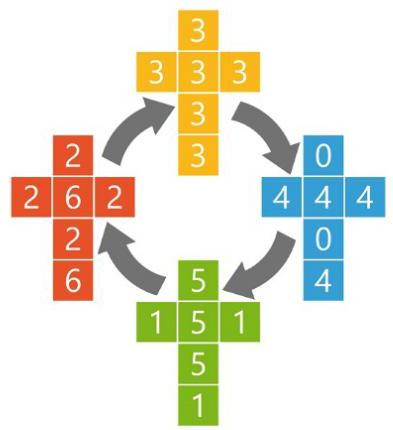
\includegraphics[max width=0.3\textwidth]{images/0194e279-9b28-703a-88f4-c3ac21e2010d_77_1048_1104_393_430_0.jpg}
\end{center}
\hspace*{3em} 

图 2.16 非传递性立方体骰子的一个示例,其中每个骰子都被“压扁”以显示每个面上的数字。这些骰子按循环排列,使得每个骰子都有 2/3 的概率掷出比循环中前一个骰子更高的数字。

2.3 (⋆) 考虑一个变量 \(\mathbf{y}\) ,它由两个独立随机变量的和给出 \(\mathbf{y} = \mathbf{u} + \mathbf{v}\) ,其中 \(\mathbf{u} \sim  {p}_{\mathbf{u}}\left( \mathbf{u}\right)\) 且 \(\mathbf{v} \sim  {p}_{\mathbf{v}}\left( \mathbf{v}\right)\) 。证明分布 \({p}_{\mathbf{y}}\left( \mathbf{y}\right)\) 由下式给出

\[
p\left( \mathbf{y}\right)  = \int {p}_{\mathbf{u}}\left( \mathbf{u}\right) {p}_{\mathbf{v}}\left( {\mathbf{y} - \mathbf{u}}\right) \mathrm{d}\mathbf{u}. \tag{2.119}
\]

这被称为 \({p}_{\mathbf{u}}\left( \mathbf{u}\right)\) 和 \({p}_{\mathbf{v}}\left( \mathbf{v}\right)\) 的卷积。

2.4 \(\left( {\star  \star  }\right)\) 验证均匀分布 (2.33) 已正确归一化,并求出其均值和方差的表达式。

2.5 (★★) 验证指数分布 (2.34) 和拉普拉斯分布 (2.35) 已正确归一化。

2.6 (*) 利用狄拉克δ函数的性质,证明经验密度 (2.37) 已正确归一化。

2.7 (*) 利用经验密度 (2.37),证明由 (2.39) 给出的期望可以近似为从形式为 (2.40) 的密度中抽取的有限样本集的求和。

2.8 (*) 利用定义 (2.44),证明 \(\operatorname{var}\left\lbrack  {f\left( x\right) }\right\rbrack\) 满足 (2.45)。

2.9 (*) 证明如果两个变量 \(x\) 和 \(y\) 相互独立,则它们的协方差为零。

2.10 (*) 假设两个变量 \(x\) 和 \(z\) 在统计上是独立的。证明它们之和的均值和方差满足

\[
\mathbb{E}\left\lbrack  {x + z}\right\rbrack   = \mathbb{E}\left\lbrack  x\right\rbrack   + \mathbb{E}\left\lbrack  z\right\rbrack   \tag{2.120}
\]

\[
\operatorname{var}\left\lbrack  {x + z}\right\rbrack   = \operatorname{var}\left\lbrack  x\right\rbrack   + \operatorname{var}\left\lbrack  z\right\rbrack  . \tag{2.121}
\]

2.11 (*) 考虑两个变量 \(x\) 和 \(y\) ,其联合分布为 \(p\left( {x,y}\right)\) 。证明以下两个结果:

\[
\mathbb{E}\left\lbrack  x\right\rbrack   = {\mathbb{E}}_{y}\left\lbrack  {{\mathbb{E}}_{x}\left\lbrack  {x \mid  y}\right\rbrack  }\right\rbrack   \tag{2.122}
\]

\[
\operatorname{var}\left\lbrack  x\right\rbrack   = {\mathbb{E}}_{y}\left\lbrack  {{\operatorname{var}}_{x}\left\lbrack  {x \mid  y}\right\rbrack  }\right\rbrack   + {\operatorname{var}}_{y}\left\lbrack  {{\mathbb{E}}_{x}\left\lbrack  {x \mid  y}\right\rbrack  }\right\rbrack  . \tag{2.123}
\]

这里 \({\mathbb{E}}_{x}\left\lbrack  {x \mid  y}\right\rbrack\) 表示在条件分布 \(p\left( {x \mid  y}\right)\) 下 \(x\) 的期望,条件方差的表示方法类似。

\({2.12}\left( {\star  \star   \star  }\right)\) 在本练习中,我们证明单变量高斯分布的归一化条件 (2.51)。为此,考虑积分

\[
I = {\int }_{-\infty }^{\infty }\exp \left( {-\frac{1}{2{\sigma }^{2}}{x}^{2}}\right) \mathrm{d}x \tag{2.124}
\]

我们可以先将其平方写成如下形式来计算

\[
{I}^{2} = {\int }_{-\infty }^{\infty }{\int }_{-\infty }^{\infty }\exp \left( {-\frac{1}{2{\sigma }^{2}}{x}^{2} - \frac{1}{2{\sigma }^{2}}{y}^{2}}\right) \mathrm{d}x\mathrm{\;d}y. \tag{2.125}
\]

现在从笛卡尔坐标 \(\left( {x,y}\right)\) 变换到极坐标 \(\left( {r,\theta }\right)\) ,然后代入 \(u = {r}^{2}\) 。证明通过对 \(\theta\) 和 \(u\) 进行积分,然后对两边取平方根,我们得到

\[
I = {\left( 2\pi {\sigma }^{2}\right) }^{1/2}. \tag{2.126}
\]

最后,利用这个结果证明高斯分布 \(\mathcal{N}\left( {x \mid  \mu ,{\sigma }^{2}}\right)\) 是归一化的。

2.13 \(\left( {\star  \star  }\right)\) 通过变量替换,验证由式 (2.49) 给出的单变量高斯分布满足式 (2.52)。接下来,对归一化

条件

\[
{\int }_{-\infty }^{\infty }\mathcal{N}\left( {x \mid  \mu ,{\sigma }^{2}}\right) \mathrm{d}x = 1 \tag{2.127}
\]

关于 \({\sigma }^{2}\) 求导,验证高斯分布满足式 (2.53)。最后,证明式 (2.54) 成立。

2.14 (⋆) 证明高斯分布 (2.49) 的众数(即最大值)由 \(\mu\) 给出。

2.15 (*) 通过令对数似然函数 (2.56) 关于 \(\mu\) 和 \({\sigma }^{2}\) 的导数等于零,验证结果 (2.57) 和 (2.58)。

2.16 \(\left( {\star  \star  }\right)\) 利用结果 (2.52) 和 (2.53),证明

\[
\mathbb{E}\left\lbrack  {{x}_{n}{x}_{m}}\right\rbrack   = {\mu }^{2} + {I}_{nm}{\sigma }^{2} \tag{2.128}
\]

其中 \({x}_{n}\) 和 \({x}_{m}\) 表示从均值为 \(\mu\) 、方差为 \({\sigma }^{2}\) 的高斯分布中采样的数据点,并且如果 \(n = m\) ,则 \({I}_{nm}\) 满足 \({I}_{nm} = 1\) ,否则满足 \({I}_{nm} = 0\) 。因此,证明结果 (2.59) 和 (2.60)。

\({2.17}\left( {\star  \star  }\right)\) 利用定义 (2.61),证明结果 (2.62),该结果表明基于真实均值的高斯分布方差估计量的期望由真实方差 \({\sigma }^{2}\) 给出。

2.18 (*) 证明关于 \({\sigma }^{2}\) 最大化 (2.66) 可得到结果 (2.68)。

2.19 \(\left( {\star  \star  }\right)\) 利用变量变换下概率密度的变换性质 (2.71),证明任何密度 \(p\left( y\right)\) 都可以通过对一个处处非零的固定密度 \(q\left( x\right)\) 进行非线性变量变换 \(y = f\left( x\right)\) 得到,其中 \(f\left( x\right)\) 是一个单调函数,使得 \(0 \leq  {f}^{\prime }\left( x\right)  < \infty\) 。写出 \(f\left( x\right)\) 满足的微分方程,并绘制一个图来说明密度的变换。

2.20 ( \(\star\) ) 计算由 (2.78) 和 (2.79) 定义的变换的雅可比矩阵的元素。

2.21 \(\left( \star \right)\) 在 2.5 节中,我们引入了熵 \(h\left( x\right)\) 的概念,它是观察具有分布 \(p\left( x\right)\) 的随机变量 \(x\) 的值所获得的信息。我们看到,对于独立变量 \(x\) 和 \(y\) ,当 \(p\left( {x,y}\right)  = p\left( x\right) p\left( y\right)\) 时,熵函数是可加的,即 \(h\left( {x,y}\right)  = h\left( x\right)  + h\left( y\right)\) 。在本题中,我们以函数 \(h\left( p\right)\) 的形式推导 \(h\) 和 \(p\) 之间的关系。首先证明 \(h\left( {p}^{2}\right)  =\)  \({2h}\left( p\right)\) ,进而通过归纳法证明 \(h\left( {p}^{n}\right)  = {nh}\left( p\right)\) ,其中 \(n\) 是正整数。因此,证明 \(h\left( {p}^{n/m}\right)  = \left( {n/m}\right) h\left( p\right)\) ,其中 \(m\) 也是正整数。这意味着 \(h\left( {p}^{x}\right)  = {xh}\left( p\right)\) ,其中 \(x\) 是正有理数,进而通过连续性可知当它是正实数时也成立。最后,证明这意味着 \(h\left( p\right)\) 必须取 \(h\left( p\right)  \propto  \ln p\) 的形式。

2.22 (★) 使用拉格朗日乘数法证明,对于离散变量,使熵(2.86)最大化会得到一个所有概率 \(p\left( {x}_{i}\right)\) 都相等的分布,此时熵的对应值为 \(\ln M\) 。

2.23 ( \(\star\) ) 考虑一个 \(M\) 状态的离散随机变量 \(x\) ,并使用形式为(2.102)的 Jensen 不等式证明其分布 \(p\left( x\right)\) 的熵满足 \(\mathrm{H}\left\lbrack  x\right\rbrack   \leq\)  \(\ln M\) 。

2.24 \(\left( {\star  \star  }\right)\) 使用变分法证明泛函(2.96)的驻点由(2.97)给出。然后使用约束条件(2.93)、(2.94)和(2.95)消除拉格朗日乘数,从而证明最大熵解由高斯分布(2.98)给出。

2.25 (★) 使用结果(2.94)和(2.95)证明单变量高斯分布(2.98)的熵由(2.99)给出。

\({2.26}\left( {\star  \star  }\right)\) 假设 \(p\left( \mathbf{x}\right)\) 是某个固定的分布,我们希望用高斯分布 \(q\left( \mathbf{x}\right)  = \mathcal{N}\left( {\mathbf{x} \mid  \mathbf{\mu },\mathbf{\sum }}\right)\) 来近似它。通过写出高斯分布 \(q\left( \mathbf{x}\right)\) 的 Kullback - Leibler 散度 \(\mathrm{{KL}}\left( {p\parallel q}\right)\) 的形式,然后求导,证明关于 \(\mathbf{\mu }\) 和 \(\mathbf{\sum }\) 最小化 \(\mathrm{{KL}}\left( {p\parallel q}\right)\) 会得到如下结果: \(\mathbf{\mu }\) 由 \(\mathbf{x}\) 在 \(p\left( \mathbf{x}\right)\) 下的期望给出, \(\mathbf{\sum }\) 由协方差给出。

2.27 \(\left( {\star  \star  }\right)\) 计算两个高斯分布 \(p\left( x\right)  = \mathcal{N}\left( {x \mid  \mu ,{\sigma }^{2}}\right)\) 和 \(q\left( x\right)  = \mathcal{N}\left( {x \mid  m,{s}^{2}}\right)\) 之间的 Kullback-Leibler 散度 (2.100)。

\({2.28}\left( {\star  \star  }\right)\) α 族散度的定义为

\[
{\mathrm{D}}_{\alpha }\left( {p\parallel q}\right)  = \frac{4}{1 - {\alpha }^{2}}\left( {1-\int p{\left( x\right) }^{\left( {1 + \alpha }\right) /2}q{\left( x\right) }^{\left( {1 - \alpha }\right) /2}\mathrm{\;d}x}\right)  \tag{2.129}
\]

其中 \(- \infty  < \alpha  < \infty\) 是一个连续参数。证明 Kullback-Leibler 散度 \(\mathrm{{KL}}\left( {p\parallel q}\right)\) 对应于 \(\alpha  \rightarrow  1\) 。这可以通过写出 \({p}^{\epsilon } =\)  \(\exp \left( {\epsilon \ln p}\right)  = 1 + \epsilon \ln p + O\left( {\epsilon }^{2}\right)\) 然后取 \(\epsilon  \rightarrow  0\) 来完成。类似地,证明 \(\mathrm{{KL}}\left( {q\parallel p}\right)\) 对应于 \(\alpha  \rightarrow   - 1\) 。

2.29 \(\left( {\star  \star  }\right)\) 考虑两个具有联合分布 \(p\left( {\mathbf{x},\mathbf{y}}\right)\) 的变量 \(\mathbf{x}\) 和 \(\mathbf{y}\) 。证明这对变量的微分熵满足

\[
\mathrm{H}\left\lbrack  {\mathbf{x},\mathbf{y}}\right\rbrack   \leq  \mathrm{H}\left\lbrack  \mathbf{x}\right\rbrack   + \mathrm{H}\left\lbrack  \mathbf{y}\right\rbrack   \tag{2.130}
\]

当且仅当 \(\mathbf{x}\) 和 \(\mathbf{y}\) 统计独立时,等号成立。

2.30 (*) 考虑一个具有分布 \(p\left( \mathbf{x}\right)\) 和相应熵 \(\mathrm{H}\left\lbrack  \mathbf{x}\right\rbrack\) 的连续变量向量 \(\mathbf{x}\) 。假设我们对 \(\mathbf{x}\) 进行非奇异线性变换以获得一个新变量 \(\mathbf{y} = \mathbf{A}\mathbf{x}\) 。证明相应的熵由 \(\mathrm{H}\left\lbrack  \mathbf{y}\right\rbrack   = \mathrm{H}\left\lbrack  \mathbf{x}\right\rbrack   + \ln \det \mathbf{A}\) 给出,其中 \(\det \mathbf{A}\) 表示 \(\mathbf{A}\) 的行列式。

2.31 \(\left( {\star  \star  }\right)\) 假设两个离散随机变量 \(x\) 和 \(y\) 之间的条件熵 \(\mathrm{H}\left\lbrack  {y \mid  x}\right\rbrack\) 为零。证明:对于所有满足 \(p\left( x\right)  > 0\) 的 \(x\) 值,变量 \(y\) 必定是 \(x\) 的函数。换句话说,对于每个 \(x\) ,只有一个 \(y\) 值满足 \(p\left( {y \mid  x}\right)  \neq  0\) 。

2.32 (★) 严格凸函数的定义是其每条弦都位于函数上方。证明这等价于函数的二阶导数为正这一条件。

2.33 (★★) 使用归纳法证明,凸函数的不等式 (2.101) 蕴含结果 (2.102)。

2.34 (★) 证明:在一个加法常数的范围内,经验分布 (2.37) 与模型分布 \(q\left( {\mathbf{x} \mid  \mathbf{\theta }}\right)\) 之间的 Kullback - Leibler 散度 (2.100) 等于负对数似然函数。

2.35 ( \(\star\) ) 结合定义 (2.107) 和概率的乘积法则,证明结果 (2.108)。

2.36 \(\left( {\star  \star   \star  }\right)\) 考虑两个二元变量 \(x\) 和 \(y\) ,其联合分布由下式给出

\begin{center}
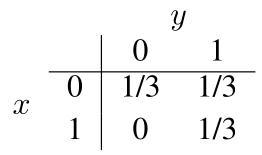
\includegraphics[max width=0.2\textwidth]{images/0194e279-9b28-703a-88f4-c3ac21e2010d_81_880_872_262_155_0.jpg}
\end{center}
\hspace*{3em} 

计算以下量:

(a) \(\mathrm{H}\left\lbrack  x\right\rbrack\) (c) \(\mathrm{H}\left\lbrack  {y \mid  x}\right\rbrack\) (e) \(\mathrm{H}\left\lbrack  {x,y}\right\rbrack\)

(b) \(\mathrm{H}\left\lbrack  y\right\rbrack\) (d) \(\mathrm{H}\left\lbrack  {x \mid  y}\right\rbrack\) (f) \(\mathrm{I}\left\lbrack  {x,y}\right\rbrack\) 。

绘制一个维恩图来展示这些不同量之间的关系。

2.37 (*) 通过应用 \(f\left( x\right)  = \ln x\) 时的詹森不等式(2.102),证明一组实数的算术平均值永远不小于它们的几何平均值。

2.38 ( \(\star\) ) 利用概率的求和与乘积规则,证明互信息 \(I\left( {\mathbf{x},\mathbf{y}}\right)\) 满足关系式(2.110)。

2.39 \(\left( {\star  \star  }\right)\) 假设两个变量 \({z}_{1}\) 和 \({z}_{2}\) 相互独立,使得 \(p\left( {{z}_{1},{z}_{2}}\right)  =\)  \(p\left( {z}_{1}\right) p\left( {z}_{2}\right)\) 。证明这些变量之间的协方差矩阵是对角矩阵。这表明独立性是两个变量不相关的充分条件。现在考虑两个变量 \({y}_{1}\) 和 \({y}_{2}\) ,其中 \({y}_{1}\) 关于 0 对称分布,且 \({y}_{2} = {y}_{1}^{2}\) 。写出条件分布 \(p\left( {{y}_{2} \mid  {y}_{1}}\right)\) ,并注意到它依赖于 \({y}_{1}\) ,从而表明这两个变量不是相互独立的。现在证明这两个变量之间的协方差矩阵仍然是对角矩阵。为此,使用关系 \(p\left( {{y}_{1},{y}_{2}}\right)  = p\left( {y}_{1}\right) p\left( {{y}_{2} \mid  {y}_{1}}\right)\) 证明非对角元素为零。这个反例表明零相关性不是独立性的充分条件。

2.40 (*) 考虑图 2.2 中的弯硬币。假设凸面为正面的先验概率是 0.1。现在假设硬币被抛掷 10 次,并且我们得知其中 8 次正面朝上,2 次反面朝上。使用贝叶斯定理评估凹面为正面的后验概率。计算下一次抛掷正面朝上的概率。

2.41 (★) 将 (2.115) 代入 (2.114) ,并利用线性回归模型对数似然的结果 (2.66) ,推导出正则化误差函数的结果 (2.117) 。

深度学习

\begin{center}
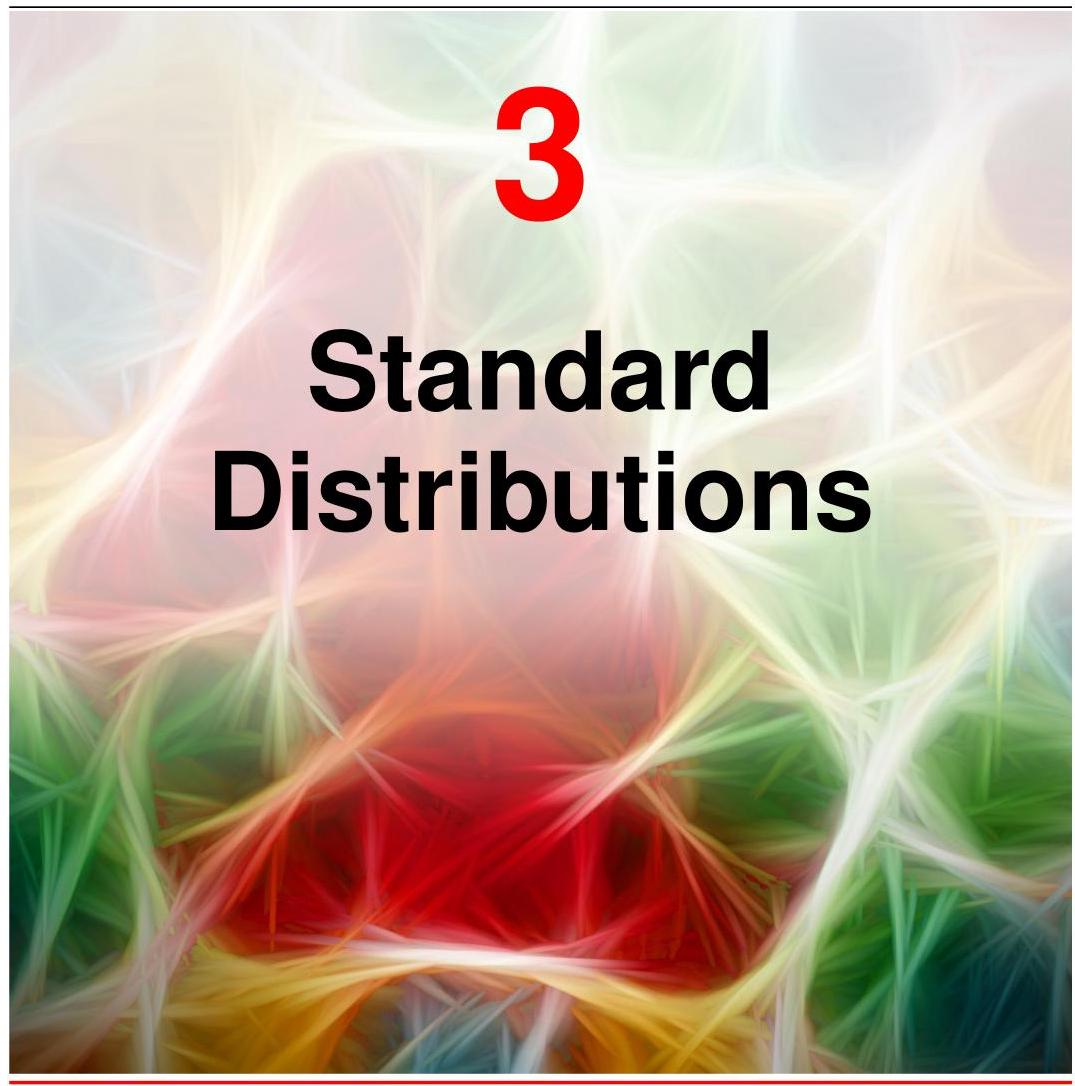
\includegraphics[max width=0.8\textwidth]{images/0194e279-9b28-703a-88f4-c3ac21e2010d_84_473_351_1075_1086_0.jpg}
\end{center}
\hspace*{3em} 

在本章中,我们将讨论一些具体的概率分布示例及其性质。这些分布本身就很有趣,同时它们也可以作为构建更复杂模型的基石,并将在整本书中被广泛使用。

本章讨论的分布的一个作用是,在给定有限观测集 \({\mathbf{x}}_{1},\ldots ,{\mathbf{x}}_{N}\) 的情况下,对随机变量 \(\mathbf{x}\) 的概率分布 \(p\left( \mathbf{x}\right)\) 进行建模。这个问题被称为密度估计。需要强调的是,密度估计问题本质上是不适定的,因为有无数种概率分布可能产生观测到的有限数据集。实际上,任何在每个数据点 \({\mathbf{x}}_{1},\ldots ,{\mathbf{x}}_{N}\) 处都不为零的分布 \(p\left( \mathbf{x}\right)\) 都是潜在的候选分布。选择合适分布的问题与模型选择问题相关,这在多项式曲线拟合的背景下已经遇到过,并且是机器学习中的一个核心问题。

\HRule

第1.2节

\HRule

我们首先考虑离散变量的分布,然后再探讨连续变量的高斯分布。这些都是参数分布的具体例子,之所以这样称呼,是因为它们由相对较少的可调整参数控制,例如高斯分布的均值和方差。为了将此类模型应用于密度估计问题,我们需要一种在给定观测数据集的情况下确定参数合适值的方法,而我们的主要关注点将是最大化似然函数。在本章中,我们将假设数据观测是独立同分布(i.i.d.)的,而在后续章节中,我们将探讨涉及结构化数据的更复杂场景,在这些场景中,这一假设不再成立。

参数方法的一个局限性在于,它假设分布具有特定的函数形式,而这对于特定应用可能并不合适。另一种方法是非参数密度估计方法,其中分布的形式通常取决于数据集的大小。此类模型仍然包含参数,但这些参数控制的是模型复杂度,而非分布的形式。本章结尾,我们将简要介绍三种分别基于直方图、最近邻和核函数的非参数方法。诸如此类非参数技术的一个主要局限性在于,它们需要存储所有的训练数据。换句话说,参数数量会随着数据集的大小而增加,因此对于大型数据集,这些方法的效率会变得非常低。深度学习通过考虑基于具有大量但固定数量参数的神经网络的灵活分布,将参数模型的效率与非参数方法的通用性相结合。

\section*{3.1. 离散变量}

我们首先考虑离散变量的简单分布,从二元变量开始,然后再讨论多状态变量。

\section*{3.1.1 伯努利分布}

考虑一个单一的二元随机变量 \(x \in  \{ 0,1\}\) 。例如, \(x\) 可能描述抛硬币的结果,其中 \(x = 1\) 表示 “正面”, \(x = 0\) 表示 “反面”。如果这是一枚有缺陷的硬币,如图 2.2 所示,那么硬币正面朝上的概率不一定与反面朝上的概率相同。 \(x = 1\) 的概率将用参数 \(\mu\) 表示,即

\[
p\left( {x = 1 \mid  \mu }\right)  = \mu  \tag{3.1}
\]

其中 \(0 \leq  \mu  \leq  1\) ,由此可得 \(p\left( {x = 0 \mid  \mu }\right)  = 1 - \mu\) 。因此, \(x\) 的概率分布可以写成如下形式

\[
\operatorname{Bern}\left( {x \mid  \mu }\right)  = {\mu }^{x}{\left( 1 - \mu \right) }^{1 - x}, \tag{3.2}
\]

\HRule

练习 3.1

\HRule

这就是所谓的伯努利分布。很容易验证,这个分布是归一化的,并且其均值和方差分别为

\[
\mathbb{E}\left\lbrack  x\right\rbrack   = \mu  \tag{3.3}
\]

\[
\operatorname{var}\left\lbrack  x\right\rbrack   = \mu \left( {1 - \mu }\right) . \tag{3.4}
\]

现在假设我们有一个数据集 \(\mathcal{D} = \left\{  {{x}_{1},\ldots ,{x}_{N}}\right\}\) ,它是 \(x\) 的观测值。我们可以构建似然函数,它是 \(\mu\) 的函数,假设这些观测值是从 \(p\left( {x \mid  \mu }\right)\) 中独立抽取的,即

\[
p\left( {\mathcal{D} \mid  \mu }\right)  = \mathop{\prod }\limits_{{n = 1}}^{N}p\left( {{x}_{n} \mid  \mu }\right)  = \mathop{\prod }\limits_{{n = 1}}^{N}{\mu }^{{x}_{n}}{\left( 1 - \mu \right) }^{1 - {x}_{n}}. \tag{3.5}
\]

我们可以通过最大化似然函数,或者等价地,通过最大化似然函数的对数来估计 \(\mu\) 的值,因为对数是一个单调函数。伯努利分布的对数似然函数为

\[
\ln p\left( {\mathcal{D} \mid  \mu }\right)  = \mathop{\sum }\limits_{{n = 1}}^{N}\ln p\left( {{x}_{n} \mid  \mu }\right)  = \mathop{\sum }\limits_{{n = 1}}^{N}\left\{  {{x}_{n}\ln \mu  + \left( {1 - {x}_{n}}\right) \ln \left( {1 - \mu }\right) }\right\}  . \tag{3.6}
\]

此时,请注意对数似然函数仅通过它们的和 \(\mathop{\sum }\limits_{n}{x}_{n}\) 依赖于 \(N\) 观测值 \({x}_{n}\) 。这个和为该分布下数据的充分统计量提供了一个示例。如果我们令 \(\ln p\left( {\mathcal{D} \mid  \mu }\right)\) 关于 \(\mu\) 的导数等于零,我们就得到了最大似然估计量:

\[
{\mu }_{\mathrm{{ML}}} = \frac{1}{N}\mathop{\sum }\limits_{{n = 1}}^{N}{x}_{n} \tag{3.7}
\]

\HRule

3.4 节

\HRule

这也被称为样本均值。用 \(m\) 表示该数据集中 \(x = 1\) (正面)的观测次数,我们可以将 (3.7) 写成如下形式

\[
{\mu }_{\mathrm{{ML}}} = \frac{m}{N} \tag{3.8}
\]

因此,在这个最大似然框架下,硬币正面朝上的概率由数据集中正面观测次数的比例给出。

\section*{3.1.2 二项分布}

我们还可以计算出给定数据集大小为 \(N\) 时, \(x = 1\) 的观测次数 \(m\) 这个二元变量 \(x\) 的分布。这被称为二项分布,从 (3.5) 我们可以看出它与 \({\mu }^{m}{\left( 1 - \mu \right) }^{N - m}\) 成比例。为了得到归一化系数,请注意在 \(N\) 次抛硬币中,我们必须将得到 \(m\) 次正面的所有可能方式相加,这样就得到了二项分布

可以写成

\[
\operatorname{Bin}\left( {m \mid  N,\mu }\right)  = \left( \begin{array}{l} N \\  m \end{array}\right) {\mu }^{m}{\left( 1 - \mu \right) }^{N - m} \tag{3.9}
\]

\begin{center}
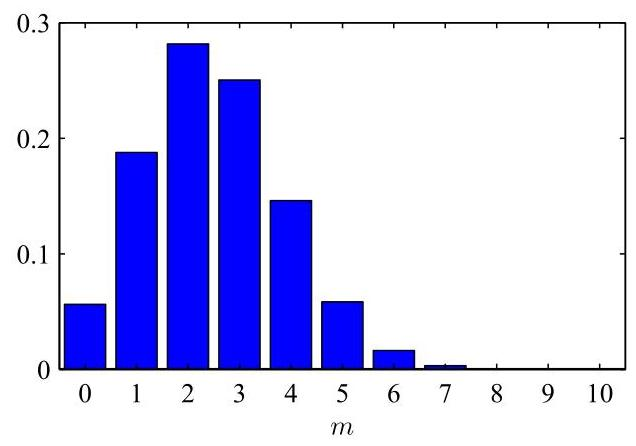
\includegraphics[max width=0.5\textwidth]{images/0194e279-9b28-703a-88f4-c3ac21e2010d_87_901_361_636_446_0.jpg}
\end{center}
\hspace*{3em} 

图 3.1 二项分布 (3.9) 作为 \(m\) 的函数的直方图,其中 \(N = {10}\) 和 \(\mu  = {0.25}\) 。

其中

\[
\left( \begin{array}{l} N \\  m \end{array}\right)  \equiv  \frac{N!}{\left( {N - m}\right) !m!} \tag{3.10}
\]

是从总共 \(N\) 个相同对象中不重复地选取 \(m\) 个对象的方式数。图 3.1 展示了 \(N = {10}\) 和 \(\mu  = {0.25}\) 时二项分布的图形。

\HRule

练习 3.3

\HRule

二项分布的均值和方差可以通过以下结果来计算:对于独立事件,和的均值等于均值的和,和的方差等于方差的和。因为 \(m = {x}_{1} + \ldots  + {x}_{N}\) ,并且对于每次观测,均值和方差分别由 (3.3) 和 (3.4) 给出,所以我们有

\[
\mathbb{E}\left\lbrack  m\right\rbrack   \equiv  \mathop{\sum }\limits_{{m = 0}}^{N}m\operatorname{Bin}\left( {m \mid  N,\mu }\right)  = {N\mu } \tag{3.11}
\]

\[
\operatorname{var}\left\lbrack  m\right\rbrack   \equiv  \mathop{\sum }\limits_{{m = 0}}^{N}{\left( m - \mathbb{E}\left\lbrack  m\right\rbrack  \right) }^{2}\operatorname{Bin}\left( {m \mid  N,\mu }\right)  = {N\mu }\left( {1 - \mu }\right) . \tag{3.12}
\]

\HRule

练习 2.10

练习 3.4

\HRule

这些结果也可以直接用微积分来证明。

\section*{3.1.3 多项分布}

二元变量可用于描述只能取两个可能值之一的量。然而,我们经常会遇到可以取 \(K\) 个可能的互斥状态之一的离散变量。虽然有多种不同的方式来表示这类变量,但我们很快会看到,一种特别方便的表示方法是 “ \(K\) 中取 1” 方案,有时也称为 “独热编码”,其中变量由一个 \(K\) 维向量 \(\mathrm{x}\) 表示,该向量中的一个元素 \({x}_{k}\) 等于 1,其余所有元素都等于 0。例如,如果我们有一个可以取 \(K = 6\) 个状态的变量,并且该变量的一个特定观测值恰好对应于 \({x}_{3} = 1\) 的状态,那么 \(\mathrm{x}\) 将表示为

\[
\mathbf{x} = {\left( 0,0,1,0,0,0\right) }^{\mathrm{T}}. \tag{3.13}
\]

注意,这样的向量满足 \(\mathop{\sum }\limits_{{k = 1}}^{K}{x}_{k} = 1\) 。如果我们用参数 \({\mu }_{k}\) 表示 \({x}_{k} = 1\) 的概率,那么 \(\mathbf{x}\) 的分布由下式给出

\[
p\left( {\mathbf{x} \mid  \mathbf{\mu }}\right)  = \mathop{\prod }\limits_{{k = 1}}^{K}{\mu }_{k}^{{x}_{k}} \tag{3.14}
\]

其中 \(\mathbf{\mu } = {\left( {\mu }_{1},\ldots ,{\mu }_{K}\right) }^{\mathrm{T}}\) ,并且参数 \({\mu }_{k}\) 被约束以满足 \({\mu }_{k} \geq  0\) 和 \(\mathop{\sum }\limits_{k}{\mu }_{k} = 1\) ,因为它们表示概率。分布 (3.14) 可以被视为伯努利分布向多于两个结果的推广。很容易看出该分布是归一化的:

\[
\mathop{\sum }\limits_{\mathbf{x}}p\left( {\mathbf{x} \mid  \mathbf{\mu }}\right)  = \mathop{\sum }\limits_{{k = 1}}^{K}{\mu }_{k} = 1 \tag{3.15}
\]

并且

\[
\mathbb{E}\left\lbrack  {\mathbf{x} \mid  \mathbf{\mu }}\right\rbrack   = \mathop{\sum }\limits_{\mathbf{x}}p\left( {\mathbf{x} \mid  \mathbf{\mu }}\right) \mathbf{x} = \mathbf{\mu }. \tag{3.16}
\]

现在考虑一个包含 \(N\) 个独立观测值 \({\mathbf{x}}_{1},\ldots ,{\mathbf{x}}_{N}\) 的数据集 \(\mathcal{D}\) 。相应的似然函数形式如下

\[
p\left( {\mathcal{D} \mid  \mathbf{\mu }}\right)  = \mathop{\prod }\limits_{{n = 1}}^{N}\mathop{\prod }\limits_{{k = 1}}^{K}{\mu }_{k}^{{x}_{nk}} = \mathop{\prod }\limits_{{k = 1}}^{K}{\mu }_{k}^{\left( \mathop{\sum }\limits_{n}{x}_{nk}\right) } = \mathop{\prod }\limits_{{k = 1}}^{K}{\mu }_{k}^{{m}_{k}} \tag{3.17}
\]

我们可以看到,似然函数仅通过 \(K\) 个量依赖于 \(N\) 个数据点:

\[
{m}_{k} = \mathop{\sum }\limits_{{n = 1}}^{N}{x}_{nk} \tag{3.18}
\]

它们表示 \({x}_{k} = 1\) 的观测数量。这些被称为该分布的充分统计量。注意,变量 \({m}_{k}\) 受以下约束

\[
\mathop{\sum }\limits_{{k = 1}}^{K}{m}_{k} = N \tag{3.19}
\]

\HRule

第 3.4 节

\HRule

为了找到 \(\mathbf{\mu }\) 的最大似然解,我们需要在考虑约束条件 (3.15)(即 \({\mu }_{k}\) 之和必须为 1)的情况下,关于 \({\mu }_{k}\) 最大化 \(\ln p\left( {\mathcal{D} \mid  \mathbf{\mu }}\right)\) 。这可以通过使用拉格朗日乘数 \(\lambda\) 并最大化来实现

\[
\mathop{\sum }\limits_{{k = 1}}^{K}{m}_{k}\ln {\mu }_{k} + \lambda \left( {\mathop{\sum }\limits_{{k = 1}}^{K}{\mu }_{k} - 1}\right) . \tag{3.20}
\]

\HRule

附录 \(C\)

\HRule

将 (3.20) 关于 \({\mu }_{k}\) 的导数设为零,我们得到

\[
{\mu }_{k} =  - {m}_{k}/\lambda  \tag{3.21}
\]

我们可以通过将 (3.21) 代入约束条件 \(\mathop{\sum }\limits_{k}{\mu }_{k} = 1\) 来求解拉格朗日乘数 \(\lambda\) ,得到 \(\lambda  =  - N\) 。因此,我们得到了

\({\mu }_{k}\) 的形式为

\[
{\mu }_{k}^{\mathrm{{ML}}} = \frac{{m}_{k}}{N}, \tag{3.22}
\]

这是 \(N\) 观测值中满足 \({x}_{k} = 1\) 的比例。

我们还可以考虑量 \({m}_{1},\ldots ,{m}_{K}\) 的联合分布,该分布以参数向量 \(\mathbf{\mu }\) 和观测总数 \(N\) 为条件。由式 (3.17) 可知,其形式为

\[
\operatorname{Mult}\left( {{m}_{1},{m}_{2},\ldots ,{m}_{K} \mid  \mathbf{\mu },N}\right)  = \left( \begin{matrix} N \\  {m}_{1}{m}_{2}\ldots {m}_{K} \end{matrix}\right) \mathop{\prod }\limits_{{k = 1}}^{K}{\mu }_{k}^{{m}_{k}}, \tag{3.23}
\]

这就是所谓的多项分布。归一化系数是将 \(N\) 个对象划分为大小为 \({m}_{1},\ldots ,{m}_{K}\) 的 \(K\) 个组的方式数,由下式给出

\[
\left( \begin{matrix} N \\  {m}_{1}{m}_{2}\ldots {m}_{K} \end{matrix}\right)  = \frac{N!}{{m}_{1}!{m}_{2}!\ldots {m}_{K}!}. \tag{3.24}
\]

请注意,二态量既可以表示为二元变量,并使用二项分布 (3.9) 进行建模,也可以表示为 2 选 1 变量,并在 \(K = 2\) 的情况下使用分布 (3.14) 进行建模。

\section*{3.2. 多元高斯分布}

高斯分布,也称为正态分布,是一种广泛用于连续变量分布的模型。我们已经知道,对于单个

第 2.3 节 变量 \(x\) ,高斯分布可以写成如下形式

\[
\mathcal{N}\left( {x \mid  \mu ,{\sigma }^{2}}\right)  = \frac{1}{{\left( 2\pi {\sigma }^{2}\right) }^{1/2}}\exp \left\{  {-\frac{1}{2{\sigma }^{2}}{\left( x - \mu \right) }^{2}}\right\}   \tag{3.25}
\]

其中 \(\mu\) 是均值, \({\sigma }^{2}\) 是方差。对于一个 \(D\) 维向量 \(\mathbf{x}\) ,多元高斯分布具有以下形式

\[
\mathcal{N}\left( {\mathbf{x} \mid  \mathbf{\mu },\mathbf{\sum }}\right)  = \frac{1}{{\left( 2\pi \right) }^{D/2}}\frac{1}{{\left| \mathbf{\sum }\right| }^{1/2}}\exp \left\{  {-\frac{1}{2}{\left( \mathbf{x} - \mathbf{\mu }\right) }^{\mathrm{T}}{\mathbf{\sum }}^{-1}\left( {\mathbf{x} - \mathbf{\mu }}\right) }\right\}   \tag{3.26}
\]

其中 \(\mathbf{\mu }\) 是 \(D\) 维均值向量, \(\mathbf{\sum }\) 是 \(D \times  D\) 协方差矩阵, \(\det \mathbf{\sum }\) 表示 \(\mathbf{\sum }\) 的行列式。

高斯分布出现在许多不同的情境中,并且可以从多种不同的视角来理解。例如,我们已经看到,对于单个实变量,使熵最大化的分布是高斯分布。

\HRule

第 2.5 节

\HRule

\begin{center}
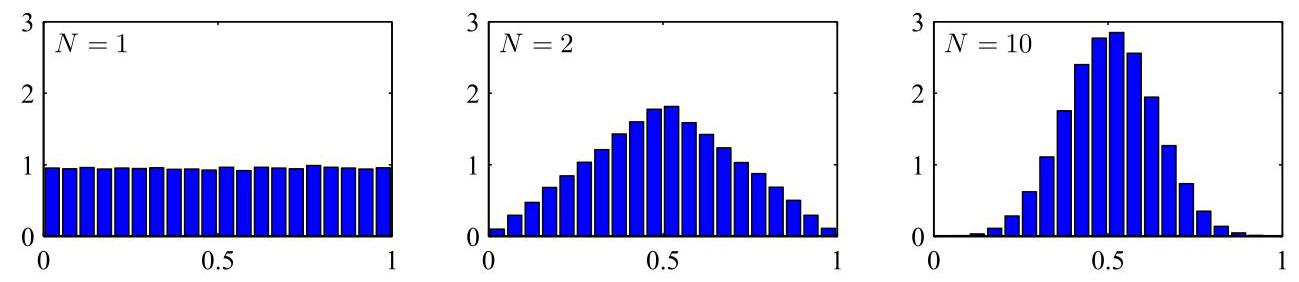
\includegraphics[max width=1.0\textwidth]{images/0194e279-9b28-703a-88f4-c3ac21e2010d_90_224_358_1299_282_0.jpg}
\end{center}
\hspace*{3em} 

图 3.2 不同 \(N\) 值下 \(N\) 个均匀分布数字的均值的直方图。我们观察到,随着 \(N\) 的增加,分布趋向于高斯分布。

练习 3.8 这个性质也适用于多元高斯分布。

高斯分布出现的另一种情况是当我们考虑多个随机变量的和时。中心极限定理告诉我们,在某些温和条件下,一组随机变量的和(它本身当然也是一个随机变量)的分布随着求和项数的增加越来越接近高斯分布(Walker,1969)。我们可以通过考虑 \(N\) 个变量 \({x}_{1},\ldots ,{x}_{N}\) 来说明这一点,每个变量在区间 \(\left\lbrack  {0,1}\right\rbrack\) 上服从均匀分布,然后考虑均值 \(\left( {{x}_{1} + \cdots  + {x}_{N}}\right) /N\) 的分布。对于较大的 \(N\) ,这个分布趋向于高斯分布,如图 3.2 所示。实际上,随着 \(N\) 的增加,向高斯分布的收敛可能非常迅速。这一结果的一个推论是,二项分布(3.9),它是由随机二元变量 \(x\) 的 \(N\) 次观测之和定义的关于 \(m\) 的分布,当 \(N \rightarrow  \infty\) 时将趋向于高斯分布(对于 \(N = {10}\) ,见图 3.1)。

高斯分布有许多重要的分析性质,我们将详细讨论其中的几个。因此,本节将比前面的一些章节在技术上更复杂,并且需要熟悉各种矩阵恒等式。

\HRule

附录 A

\HRule

\section*{3.2.1 高斯分布的几何性质}

我们首先考虑高斯分布的几何形式。高斯分布对 \(\mathbf{x}\) 的函数依赖是通过二次型实现的

\[
{\Delta }^{2} = {\left( \mathbf{x} - \mathbf{\mu }\right) }^{\mathrm{T}}{\mathbf{\sum }}^{-1}\left( {\mathbf{x} - \mathbf{\mu }}\right) , \tag{3.27}
\]

它出现在指数中。量 \(\Delta\) 被称为从 \(\mathbf{\mu }\) 到 \(\mathbf{x}\) 的马氏距离。当 \(\mathbf{\sum }\) 是单位矩阵时,它简化为欧几里得距离。在 \(\mathbf{x}\) 空间中,对于二次型为常数的曲面,高斯分布是常数。

首先,注意到不失一般性,矩阵 \(\mathbf{\sum }\) 可以被视为对称矩阵,因为任何反对称分量都会从指数中消失。现在考虑协方差矩阵的特征向量方程

\[
\sum {\mathbf{u}}_{i} = {\lambda }_{i}{\mathbf{u}}_{i} \tag{3.28}
\]

\HRule

练习 3.11

\HRule

其中 \(i = 1,\ldots ,D\) 。因为 \(\mathbf{\sum }\) 是一个实对称矩阵,其特征值将是实数,并且可以选择其特征向量构成一个标准正交基,使得

\[
{\mathbf{u}}_{i}^{\mathrm{T}}{\mathbf{u}}_{j} = {I}_{ij} \tag{3.29}
\]

\HRule

练习 3.12

\HRule

其中 \({I}_{ij}\) 是单位矩阵的 \(i,j\) 元素,并且满足

\[
{I}_{ij} = \left\{  \begin{array}{ll} 1, & \text{ if }i = j \\  0, & \text{ otherwise. } \end{array}\right.  \tag{3.30}
\]

协方差矩阵 \(\mathbf{\sum }\) 可以用其特征向量展开的形式表示为

\[
\mathbf{\sum } = \mathop{\sum }\limits_{{i = 1}}^{D}{\lambda }_{i}{\mathbf{u}}_{i}{\mathbf{u}}_{i}^{\mathrm{T}} \tag{3.31}
\]

\HRule

练习 3.13

\HRule

类似地,逆协方差矩阵 \({\mathbf{\sum }}^{-1}\) 可以表示为

\[
{\mathbf{\sum }}^{-1} = \mathop{\sum }\limits_{{i = 1}}^{D}\frac{1}{{\lambda }_{i}}{\mathbf{u}}_{i}{\mathbf{u}}_{i}^{\mathrm{T}}. \tag{3.32}
\]

将 (3.32) 代入 (3.27),二次型变为

\[
{\Delta }^{2} = \mathop{\sum }\limits_{{i = 1}}^{D}\frac{{y}_{i}^{2}}{{\lambda }_{i}} \tag{3.33}
\]

其中我们定义了

\[
{y}_{i} = {\mathbf{u}}_{i}^{\mathrm{T}}\left( {\mathbf{x} - \mathbf{\mu }}\right) . \tag{3.34}
\]

我们可以将 \(\left\{  {y}_{i}\right\}\) 解释为一个由正交归一向量 \({\mathbf{u}}_{i}\) 定义的新坐标系,该坐标系相对于原始的 \({x}_{i}\) 坐标进行了平移和旋转。构造向量 \(\mathbf{y} = {\left( {y}_{1},\ldots ,{y}_{D}\right) }^{\mathrm{T}}\) ,我们有

\[
\mathbf{y} = \mathbf{U}\left( {\mathbf{x} - \mathbf{\mu }}\right)  \tag{3.35}
\]

其中 \(\mathbf{U}\) 是一个矩阵,其行由 \({\mathbf{u}}_{i}^{\mathrm{T}}\) 给出。由 (3.29) 可知, \(\mathbf{U}\) 是一个正交矩阵,即它满足 \(\mathbf{U}{\mathbf{U}}^{\mathrm{T}} = {\mathbf{U}}^{\mathrm{T}}\mathbf{U} = \mathbf{I}\) ,其中 \(\mathbf{I}\) 是单位矩阵。

\HRule

附录 A

\HRule

二次型,进而高斯密度,在 (3.33) 为常数的曲面上是恒定的。如果所有特征值 \({\lambda }_{i}\) 都是正的,那么这些曲面表示椭球体,其中心位于 \(\mathbf{\mu }\) ,轴沿着 \({\mathbf{u}}_{i}\) 方向,并且轴方向的缩放因子由 \({\lambda }_{i}^{1/2}\) 给出,如图 3.3 所示。

为了使高斯分布有良好的定义,协方差矩阵的所有特征值 \({\lambda }_{i}\) 必须严格为正,否则该分布无法正确归一化。特征值严格为正的矩阵称为正定矩阵。当我们讨论潜在变量模型时,会遇到一个或多个特征值为零的高斯分布,在这种情况下,分布是奇异的,并且局限于一个低维子空间。如果所有特征值都是非负的,那么协方差矩阵称为半正定矩阵。

\HRule

第 16 章

\HRule

\begin{center}
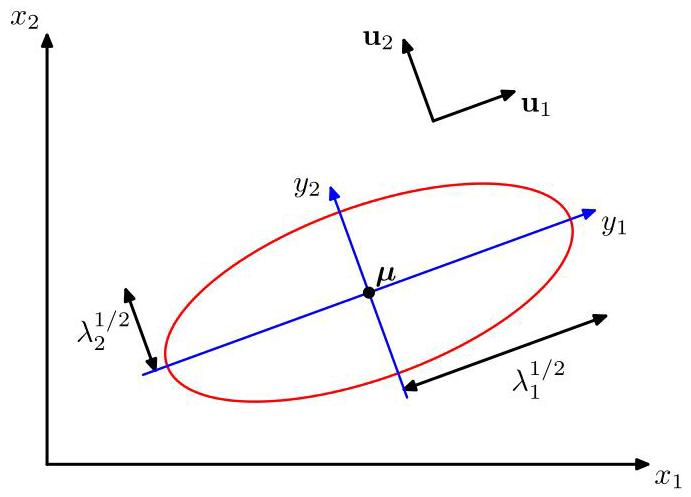
\includegraphics[max width=0.5\textwidth]{images/0194e279-9b28-703a-88f4-c3ac21e2010d_92_854_346_691_497_0.jpg}
\end{center}
\hspace*{3em} 

图 3.3 红色曲线展示了二维空间 \(\mathbf{x} =\)  \(\left( {{x}_{1},{x}_{2}}\right)\) 中高斯分布的恒定概率密度椭圆曲面,在该曲面上的密度是其在 \(\mathbf{x} =\)  \(\mu\) 处值的 \(\exp \left( {-1/2}\right)\) 倍。椭圆的轴由协方差矩阵的特征向量 \({\mathbf{u}}_{i}\) 定义,对应的特征值为 \({\lambda }_{i}\) 。

现在考虑由 \({y}_{i}\) 定义的新坐标系中高斯分布的形式。从 \(\mathbf{x}\) 坐标系转换到 \(\mathbf{y}\) 坐标系时,我们有一个雅可比矩阵 \(\mathbf{J}\) ,其元素由下式给出

\[
{J}_{ij} = \frac{\partial {x}_{i}}{\partial {y}_{j}} = {U}_{ji} \tag{3.36}
\]

其中 \({U}_{ji}\) 是矩阵 \({\mathbf{U}}^{\mathrm{T}}\) 的元素。利用矩阵 \(\mathbf{U}\) 的正交归一性,我们可以看到雅可比矩阵行列式的平方为

\[
{\left| \mathbf{J}\right| }^{2} = {\left| {\mathbf{U}}^{\mathrm{T}}\right| }^{2} = \left| {\mathbf{U}}^{\mathrm{T}}\right| \left| \mathbf{U}\right|  = \left| {{\mathbf{U}}^{\mathrm{T}}\mathbf{U}}\right|  = \left| \mathbf{I}\right|  = 1 \tag{3.37}
\]

因此, \(\left| \mathbf{J}\right|  = 1\) 。此外,协方差矩阵的行列式 \(\left| \mathbf{\sum }\right|\) 可以写成其特征值的乘积,因此

\[
{\left| \mathbf{\sum }\right| }^{1/2} = \mathop{\prod }\limits_{{j = 1}}^{D}{\lambda }_{j}^{1/2} \tag{3.38}
\]

因此,在 \({y}_{j}\) 坐标系中,高斯分布具有以下形式

\[
p\left( \mathbf{y}\right)  = p\left( \mathbf{x}\right) \left| \mathbf{J}\right|  = \mathop{\prod }\limits_{{j = 1}}^{D}\frac{1}{{\left( 2\pi {\lambda }_{j}\right) }^{1/2}}\exp \left\{  {-\frac{{y}_{j}^{2}}{2{\lambda }_{j}}}\right\}  , \tag{3.39}
\]

这是 \(D\) 个独立的单变量高斯分布的乘积。因此,特征向量定义了一组新的平移和旋转后的坐标,相对于这些坐标,联合概率分布可以分解为独立分布的乘积。在 \(\mathbf{y}\) 坐标系中,该分布的积分为

\[
\int p\left( \mathbf{y}\right) \mathrm{d}\mathbf{y} = \mathop{\prod }\limits_{{j = 1}}^{D}{\int }_{-\infty }^{\infty }\frac{1}{{\left( 2\pi {\lambda }_{j}\right) }^{1/2}}\exp \left\{  {-\frac{{y}_{j}^{2}}{2{\lambda }_{j}}}\right\}  \mathrm{d}{y}_{j} = 1 \tag{3.40}
\]

这里我们使用了单变量高斯分布归一化的结果 (2.51)。这证实了多元高斯分布 (3.26) 确实是归一化的。

\section*{3.2.2 矩}

现在我们来研究高斯分布的矩,从而对参数 \(\mathbf{\mu }\) 和 \(\mathbf{\sum }\) 给出一种解释。在高斯分布下 \(\mathbf{x}\) 的期望由下式给出

\[
\mathbb{E}\left\lbrack  \mathbf{x}\right\rbrack   = \frac{1}{{\left( 2\pi \right) }^{D/2}}\frac{1}{{\left| \mathbf{\sum }\right| }^{1/2}}\int \exp \left\{  {-\frac{1}{2}{\left( \mathbf{x} - \mathbf{\mu }\right) }^{\mathrm{T}}{\mathbf{\sum }}^{-1}\left( {\mathbf{x} - \mathbf{\mu }}\right) }\right\}  \mathbf{x}\mathrm{d}\mathbf{x}
\]

\[
= \frac{1}{{\left( 2\pi \right) }^{D/2}}\frac{1}{{\left| \mathbf{\sum }\right| }^{1/2}}\int \exp \left\{  {-\frac{1}{2}{\mathbf{z}}^{\mathrm{T}}{\mathbf{\sum }}^{-1}\mathbf{z}}\right\}  \left( {\mathbf{z} + \mathbf{\mu }}\right) \mathrm{d}\mathbf{z} \tag{3.41}
\]

这里我们使用 \(\mathbf{z} = \mathbf{x} - \mathbf{\mu }\) 进行了变量替换。注意,指数是 \(\mathbf{z}\) 各分量的偶函数,并且由于对这些分量的积分范围是 \(\left( {-\infty ,\infty }\right)\) ,因子 \(\left( {\mathbf{z} + \mathbf{\mu }}\right)\) 中涉及 \(\mathbf{z}\) 的项将由于对称性而消失。因此,

\[
\mathbb{E}\left\lbrack  \mathbf{x}\right\rbrack   = \mathbf{\mu } \tag{3.42}
\]

所以我们将 \(\mathbf{\mu }\) 称为高斯分布的均值。

现在我们考虑高斯分布的二阶矩。在单变量情况下,我们考虑由 \(\mathbb{E}\left\lbrack  {x}^{2}\right\rbrack\) 给出的二阶矩。对于多变量高斯分布,有 \({D}^{2}\) 个由 \(\mathbb{E}\left\lbrack  {{x}_{i}{x}_{j}}\right\rbrack\) 给出的二阶矩,我们可以将它们组合在一起形成矩阵 \(\mathbb{E}\left\lbrack  {\mathbf{{xx}}}^{\mathrm{T}}\right\rbrack\) 。这个矩阵可以写成

\[
\mathbb{E}\left\lbrack  {\mathbf{{xx}}}^{\mathrm{T}}\right\rbrack   = \frac{1}{{\left( 2\pi \right) }^{D/2}}\frac{1}{{\left| \mathbf{\sum }\right| }^{1/2}}\int \exp \left\{  {-\frac{1}{2}{\left( \mathbf{x} - \mathbf{\mu }\right) }^{\mathrm{T}}{\mathbf{\sum }}^{-1}\left( {\mathbf{x} - \mathbf{\mu }}\right) }\right\}  {\mathbf{{xx}}}^{\mathrm{T}}\mathrm{d}\mathbf{x}
\]

\[
= \frac{1}{{\left( 2\pi \right) }^{D/2}}\frac{1}{{\left| \mathbf{\sum }\right| }^{1/2}}\int \exp \left\{  {-\frac{1}{2}{\mathbf{z}}^{\mathrm{T}}{\mathbf{\sum }}^{-1}\mathbf{z}}\right\}  \left( {\mathbf{z} + \mathbf{\mu }}\right) {\left( \mathbf{z} + \mathbf{\mu }\right) }^{\mathrm{T}}\mathrm{d}\mathbf{z} \tag{3.43}
\]

这里我们再次使用 \(\mathbf{z} = \mathbf{x} - \mathbf{\mu }\) 进行了变量替换。注意,涉及 \(\mathbf{\mu }{\mathbf{z}}^{\mathrm{T}}\) 和 \({\mathbf{\mu }}^{\mathrm{T}}\mathbf{z}\) 的交叉项将再次由于对称性而消失。项 \(\mathbf{\mu }{\mathbf{\mu }}^{\mathrm{T}}\) 是常数,可以提到积分外面,由于高斯分布是归一化的,积分本身的值为 1。考虑涉及 \({\mathbf{{zz}}}^{\mathrm{T}}\) 的项。同样,我们可以利用由 (3.28) 给出的协方差矩阵的特征向量展开,再结合特征向量集的完备性,写成

\[
\mathbf{z} = \mathop{\sum }\limits_{{j = 1}}^{D}{y}_{j}{\mathbf{u}}_{j} \tag{3.44}
\]

其中 \({y}_{j} = {\mathbf{u}}_{j}^{\mathrm{T}}\mathbf{z}\) ,由此可得

\[
\frac{1}{{\left( 2\pi \right) }^{D/2}}\frac{1}{{\left| \mathbf{\sum }\right| }^{1/2}}\int \exp \left\{  {-\frac{1}{2}{\mathbf{z}}^{\mathrm{T}}{\mathbf{\sum }}^{-1}\mathbf{z}}\right\}  \mathbf{z}{\mathbf{z}}^{\mathrm{T}}\mathrm{d}\mathbf{z}
\]

\[
= \frac{1}{{\left( 2\pi \right) }^{D/2}}\frac{1}{{\left| \mathbf{\sum }\right| }^{1/2}}\mathop{\sum }\limits_{{i = 1}}^{D}\mathop{\sum }\limits_{{j = 1}}^{D}{\mathbf{u}}_{i}{\mathbf{u}}_{j}^{\mathrm{T}}\int \exp \left\{  {-\mathop{\sum }\limits_{{k = 1}}^{D}\frac{{y}_{k}^{2}}{2{\lambda }_{k}}}\right\}  {y}_{i}{y}_{j}\mathrm{\;d}\mathbf{y}
\]

\[
= \mathop{\sum }\limits_{{i = 1}}^{D}{\mathbf{u}}_{i}{\mathbf{u}}_{i}^{\mathrm{T}}{\lambda }_{i} = \mathbf{\sum } \tag{3.45}
\]

在此我们利用了特征向量方程 (3.28),以及中间一行的积分由于对称性而消失的事实,除非 \(i = j\) 。在最后一行,我们利用了结果 (2.53) 和 (3.38),以及 (3.31)。因此,我们得到

\[
\mathbb{E}\left\lbrack  {\mathbf{x}{\mathbf{x}}^{\mathrm{T}}}\right\rbrack   = \mathbf{\mu }{\mathbf{\mu }}^{\mathrm{T}} + \mathbf{\sum }. \tag{3.46}
\]

在定义单个随机变量的方差时,我们在取二阶矩之前减去了均值。类似地,在多变量的情况下,减去均值仍然很方便,从而引出了随机向量的协方差

\(\mathrm{x}\) 定义为

\[
\operatorname{cov}\left\lbrack  \mathbf{x}\right\rbrack   = \mathbb{E}\left\lbrack  {\left( {\mathbf{x} - \mathbb{E}\left\lbrack  \mathbf{x}\right\rbrack  }\right) {\left( \mathbf{x} - \mathbb{E}\left\lbrack  \mathbf{x}\right\rbrack  \right) }^{\mathrm{T}}}\right\rbrack  . \tag{3.47}
\]

对于高斯分布的特定情况,我们可以利用 \(\mathbb{E}\left\lbrack  \mathbf{x}\right\rbrack   = \mathbf{\mu }\) 以及结果 (3.46),得到

\[
\operatorname{cov}\left\lbrack  \mathbf{x}\right\rbrack   = \mathbf{\sum }. \tag{3.48}
\]

由于参数矩阵 \(\mathbf{\sum }\) 控制着高斯分布下 \(\mathbf{x}\) 的协方差,因此它被称为协方差矩阵。

\section*{3.2.3 局限性}

尽管高斯分布(3.26)常被用作简单的密度模型,但它存在一些显著的局限性。考虑该分布中的自由参数数量。一个一般的对称协方差矩阵 \(\mathbf{\sum }\) 将有 \(D\left( {D + 1}\right) /2\) 个独立参数,并且在 \(\mathbf{\mu }\) 中还有另外 \(D\) 个独立参数,总共给出 \(D\left( {D + 3}\right) /2\) 个参数。对于较大的 \(D\) ,参数总数因此随 \(D\) 呈二次增长,处理和求逆大型矩阵的计算任务可能变得难以承受。解决这个问题的一种方法是使用协方差矩阵的受限形式。如果我们考虑对角协方差矩阵,使得 \(\mathbf{\sum } = \operatorname{diag}\left( {\sigma }_{i}^{2}\right)\) ,那么我们在密度模型中总共有 \({2D}\) 个独立参数。相应的等密度轮廓由与坐标轴对齐的椭球体给出。我们可以进一步将协方差矩阵限制为与单位矩阵成比例,即 \(\mathbf{\sum } = {\sigma }^{2}\mathbf{I}\) ,称为各向同性协方差,在模型中给出 \(D + 1\) 个独立参数以及等密度的球面。一般、对角和各向同性协方差矩阵的三种可能性如图 3.4 所示。不幸的是,虽然这些方法限制了分布中的自由度数量,并使协方差矩阵的求逆操作快得多,但它们也极大地限制了概率密度的形式,并限制了其捕捉数据中有趣相关性的能力。

\HRule

练习 3.15

\HRule

\begin{center}
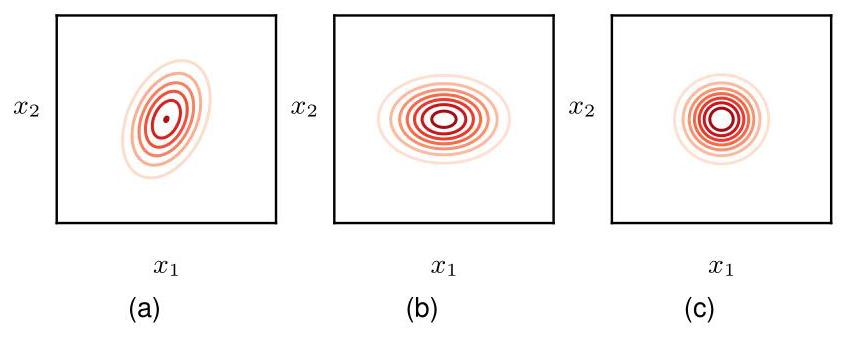
\includegraphics[max width=0.6\textwidth]{images/0194e279-9b28-703a-88f4-c3ac21e2010d_95_699_344_842_337_0.jpg}
\end{center}
\hspace*{3em} 

图 3.4 二维高斯分布的等概率密度轮廓,其中协方差矩阵为(a)一般形式,(b)对角形式,在这种情况下椭圆轮廓与坐标轴对齐,以及(c)与单位矩阵成比例,在这种情况下轮廓为同心圆。

高斯分布的另一个局限性是它本质上是单峰的(即只有一个最大值),因此无法很好地近似多峰分布。因此,高斯分布可能既过于灵活(从参数过多的意义上来说),又在其能够充分表示的分布范围上过于受限。我们稍后将看到,引入潜在变量(也称为隐藏变量或未观测变量)可以解决这两个问题。特别是,通过引入离散潜在变量得到了一个丰富的多峰分布族,从而产生了高斯混合模型。类似地,引入连续潜在变量会得到这样的模型,其中自由参数的数量可以独立于数据空间的维度 \(D\) 进行控制,同时仍然允许模型捕捉数据集中的主要相关性。

\HRule

第 3.2.9 节

第 16 章

\HRule

\section*{3.2.4 条件分布}

多元高斯分布的一个重要性质是,如果两组变量是联合高斯分布,那么一组变量在另一组变量条件下的条件分布仍然是高斯分布。同样,任一组变量的边缘分布也是高斯分布。

首先,考虑条件分布的情况。假设 \(\mathbf{x}\) 是一个服从高斯分布 \(\mathcal{N}\left( {\mathbf{x} \mid  \mathbf{\mu },\mathbf{\sum }}\right)\) 的 \(D\) 维向量,并且我们将 \(\mathbf{x}\) 划分为两个不相交的子集 \({\mathbf{x}}_{a}\) 和 \({\mathbf{x}}_{b}\) 。不失一般性,我们可以取 \({\mathbf{x}}_{a}\) 构成 \(\mathbf{x}\) 的前 \(M\) 个分量, \({\mathbf{x}}_{b}\) 包含其余的 \(D - M\) 个分量,使得

\[
\mathbf{x} = \left( \begin{array}{l} {\mathbf{x}}_{a} \\  {\mathbf{x}}_{b} \end{array}\right) . \tag{3.49}
\]

我们还定义均值向量 \(\mathbf{\mu }\) 的相应划分如下

\[
\mathbf{\mu } = \left( \begin{array}{l} {\mathbf{\mu }}_{a} \\  {\mathbf{\mu }}_{b} \end{array}\right)  \tag{3.50}
\]

以及协方差矩阵 \(\mathbf{\sum }\) 的相应划分如下

\[
\mathbf{\sum } = \left( \begin{array}{ll} {\mathbf{\sum }}_{aa} & {\mathbf{\sum }}_{ab} \\  {\mathbf{\sum }}_{ba} & {\mathbf{\sum }}_{bb} \end{array}\right) . \tag{3.51}
\]

注意,协方差矩阵的对称性 \({\mathbf{\sum }}^{\mathrm{T}} = \mathbf{\sum }\) 意味着 \({\mathbf{\sum }}_{aa}\) 和 \({\mathbf{\sum }}_{bb}\) 是对称的,并且 \({\mathbf{\sum }}_{ba} = {\mathbf{\sum }}_{ab}^{\mathrm{T}}\) 。

在许多情况下,使用协方差矩阵的逆矩阵会很方便:

\[
\mathbf{\Lambda } \equiv  {\mathbf{\sum }}^{-1}, \tag{3.52}
\]

它被称为精度矩阵。事实上,我们将看到,高斯分布的一些性质用协方差来表达最为自然,而另一些性质用精度来表达则形式更简单。因此,我们也引入精度矩阵的分块形式:

\[
\mathbf{\Lambda } = \left( \begin{array}{ll} {\mathbf{\Lambda }}_{aa} & {\mathbf{\Lambda }}_{ab} \\  {\mathbf{\Lambda }}_{ba} & {\mathbf{\Lambda }}_{bb} \end{array}\right)  \tag{3.53}
\]

对应于向量 \(\mathbf{x}\) 的分块 (3.49)。由于对称矩阵的逆矩阵也是对称的,我们可以看到 \({\mathbf{\Lambda }}_{aa}\) 和 \({\mathbf{\Lambda }}_{bb}\) 是对称的,并且 \({\mathbf{\Lambda }}_{ba} = {\mathbf{\Lambda }}_{ab}^{\mathrm{T}}\) 。此时需要强调的是,例如, \({\mathbf{\Lambda }}_{aa}\) 并非简单地由 \({\mathbf{\sum }}_{aa}\) 的逆矩阵给出。事实上,我们很快将研究分块矩阵的逆矩阵与其各分块的逆矩阵之间的关系。

\HRule

练习 3.16

\HRule

我们首先来推导条件分布 \(p\left( {{\mathbf{x}}_{a} \mid  {\mathbf{x}}_{b}}\right)\) 的表达式。根据概率的乘积规则,我们知道可以通过将联合分布 \(p\left( \mathbf{x}\right)  = p\left( {{\mathbf{x}}_{a},{\mathbf{x}}_{b}}\right)\) 中的 \({\mathbf{x}}_{b}\) 固定为观测值,并对得到的表达式进行归一化处理,从而得到关于 \({\mathbf{x}}_{a}\) 的有效概率分布,以此来计算这个条件分布。我们无需显式地进行归一化操作,而是可以通过考虑由 (3.27) 给出的高斯分布指数中的二次型,然后在计算结束时恢复归一化系数,从而更高效地得到解。如果我们利用分块 (3.49)、(3.50) 和 (3.53),就可以得到

\[
- \frac{1}{2}{\left( \mathbf{x} - \mathbf{\mu }\right) }^{\mathrm{T}}{\mathbf{\sum }}^{-1}\left( {\mathbf{x} - \mathbf{\mu }}\right)  =
\]

\[
- \frac{1}{2}{\left( {\mathbf{x}}_{a} - {\mathbf{\mu }}_{a}\right) }^{\mathrm{T}}{\mathbf{\Lambda }}_{aa}\left( {{\mathbf{x}}_{a} - {\mathbf{\mu }}_{a}}\right)  - \frac{1}{2}{\left( {\mathbf{x}}_{a} - {\mathbf{\mu }}_{a}\right) }^{\mathrm{T}}{\mathbf{\Lambda }}_{ab}\left( {{\mathbf{x}}_{b} - {\mathbf{\mu }}_{b}}\right)
\]

\[
- \frac{1}{2}{\left( {\mathbf{x}}_{b} - {\mathbf{\mu }}_{b}\right) }^{\mathrm{T}}{\mathbf{\Lambda }}_{ba}\left( {{\mathbf{x}}_{a} - {\mathbf{\mu }}_{a}}\right)  - \frac{1}{2}{\left( {\mathbf{x}}_{b} - {\mathbf{\mu }}_{b}\right) }^{\mathrm{T}}{\mathbf{\Lambda }}_{bb}\left( {{\mathbf{x}}_{b} - {\mathbf{\mu }}_{b}}\right) . \tag{3.54}
\]

我们看到,作为 \({\mathrm{x}}_{a}\) 的函数,这又是一个二次型,因此,相应的条件分布 \(p\left( {{\mathbf{x}}_{a} \mid  {\mathbf{x}}_{b}}\right)\) 将是高斯分布。由于这个分布完全由其均值和协方差来表征,我们的目标将是通过观察 (3.54) 来确定 \(p\left( {{\mathbf{x}}_{a} \mid  {\mathbf{x}}_{b}}\right)\) 的均值和协方差的表达式。

这是一个与高斯分布相关的相当常见的运算示例,有时称为“配方法”。在这个示例中,我们得到一个定义高斯分布中指数项的二次型,并且需要确定相应的均值和协方差。通过注意到一般高斯分布 \(\mathcal{N}\left( {\mathbf{x} \mid  \mathbf{\mu },\mathbf{\sum }}\right)\) 中的指数可以写成如下形式,这类问题可以直接得到解决

\[
- \frac{1}{2}{\left( \mathbf{x} - \mathbf{\mu }\right) }^{\mathrm{T}}{\mathbf{\sum }}^{-1}\left( {\mathbf{x} - \mathbf{\mu }}\right)  =  - \frac{1}{2}{\mathbf{x}}^{\mathrm{T}}{\mathbf{\sum }}^{-1}\mathbf{x} + {\mathbf{x}}^{\mathrm{T}}{\mathbf{\sum }}^{-1}\mathbf{\mu } + \text{ const } \tag{3.55}
\]

其中 'const' 表示与 \(\mathbf{x}\) 无关的项。我们还利用了 \(\sum\) 的对称性。因此,如果我们取一般的二次型并将其表示为 (3.55) 式右侧的形式,那么我们可以立即将 \(\mathrm{x}\) 中二阶项的系数矩阵等同于逆协方差矩阵 \({\mathbf{\sum }}^{-1}\) ,并将 \(\mathbf{x}\) 中线性项的系数等同于 \({\mathbf{\sum }}^{-1}\mathbf{\mu }\) ,由此我们可以得到 \(\mu\) 。

现在让我们将这个过程应用于条件高斯分布 \(p\left( {{\mathbf{x}}_{a} \mid  {\mathbf{x}}_{b}}\right)\) ,其指数中的二次型由 (3.54) 式给出。我们分别用 \({\mathbf{\mu }}_{a \mid  b}\) 和 \({\mathbf{\sum }}_{a \mid  b}\) 表示这个分布的均值和协方差。考虑 (3.54) 式对 \({\mathbf{x}}_{a}\) 的函数依赖关系,其中 \({\mathbf{x}}_{b}\) 被视为常数。如果我们挑出 \({\mathbf{x}}_{a}\) 的所有二阶项,我们得到

\[
- \frac{1}{2}{\mathbf{x}}_{a}^{\mathrm{T}}{\mathbf{\Lambda }}_{aa}{\mathbf{x}}_{a} \tag{3.56}
\]

由此我们可以立即得出 \(p\left( {{\mathbf{x}}_{a} \mid  {\mathbf{x}}_{b}}\right)\) 的协方差(逆精度)由下式给出

\[
{\mathbf{\sum }}_{a \mid  b} = {\mathbf{\Lambda }}_{aa}^{-1}. \tag{3.57}
\]

现在考虑 (3.54) 式中所有关于 \({\mathbf{x}}_{a}\) 的线性项:

\[
{\mathbf{x}}_{a}^{\mathrm{T}}\left\{  {{\mathbf{\Lambda }}_{aa}{\mathbf{\mu }}_{a} - {\mathbf{\Lambda }}_{ab}\left( {{\mathbf{x}}_{b} - {\mathbf{\mu }}_{b}}\right) }\right\}   \tag{3.58}
\]

其中我们使用了 \({\mathbf{\Lambda }}_{ba}^{\mathrm{T}} = {\mathbf{\Lambda }}_{ab}\) 。根据我们对一般形式 (3.55) 的讨论,这个表达式中 \({\mathbf{x}}_{a}\) 的系数必须等于 \({\mathbf{\sum }}_{a \mid  b}^{-1}{\mathbf{\mu }}_{a \mid  b}\) ,因此,

\[
{\mathbf{\mu }}_{a \mid  b} = {\mathbf{\sum }}_{a \mid  b}\left\{  {{\mathbf{\Lambda }}_{aa}{\mathbf{\mu }}_{a} - {\mathbf{\Lambda }}_{ab}\left( {{\mathbf{x}}_{b} - {\mathbf{\mu }}_{b}}\right) }\right\}
\]

\[
= {\mathbf{\mu }}_{a} - {\mathbf{\Lambda }}_{aa}^{-1}{\mathbf{\Lambda }}_{ab}\left( {{\mathbf{x}}_{b} - {\mathbf{\mu }}_{b}}\right)  \tag{3.59}
\]

这里我们利用了式(3.57)。

结果(3.57)和(3.59)是用原始联合分布 \(p\left( {{\mathbf{x}}_{a},{\mathbf{x}}_{b}}\right)\) 的分块精度矩阵表示的。我们也可以用相应的分块协方差矩阵来表示这些结果。为此,我们利用分块矩阵求逆的以下恒等式:

\[
{\left( \begin{array}{ll} \mathbf{A} & \mathbf{B} \\  \mathbf{C} & \mathbf{D} \end{array}\right) }^{-1} = \left( \begin{matrix} \mathbf{M} &  - \mathbf{{MB}}{\mathbf{D}}^{-1} \\   - {\mathbf{D}}^{-1}\mathbf{{CM}} & {\mathbf{D}}^{-1} + {\mathbf{D}}^{-1}\mathbf{{CMB}}{\mathbf{D}}^{-1} \end{matrix}\right)  \tag{3.60}
\]

\HRule

练习3.18

\HRule

这里我们定义了

\[
\mathbf{M} = {\left( \mathbf{A} - {\mathbf{{BD}}}^{-1}\mathbf{C}\right) }^{-1}. \tag{3.61}
\]

量 \({\mathbf{M}}^{-1}\) 被称为式(3.60)左边矩阵关于子矩阵 D 的舒尔补。利用该定义

\[
{\left( \begin{matrix} {\mathbf{\sum }}_{aa} & {\mathbf{\sum }}_{ab} \\  {\mathbf{\sum }}_{ba} & {\mathbf{\sum }}_{bb} \end{matrix}\right) }^{-1} = \left( \begin{matrix} {\mathbf{\Lambda }}_{aa} & {\mathbf{\Lambda }}_{ab} \\  {\mathbf{\Lambda }}_{ba} & {\mathbf{\Lambda }}_{bb} \end{matrix}\right)  \tag{3.62}
\]

并利用式(3.60),我们得到

\[
{\mathbf{\Lambda }}_{aa} = {\left( {\mathbf{\sum }}_{aa} - {\mathbf{\sum }}_{ab}{\mathbf{\sum }}_{bb}^{-1}{\mathbf{\sum }}_{ba}\right) }^{-1} \tag{3.63}
\]

\[
{\mathbf{\Lambda }}_{ab} =  - {\left( {\mathbf{\sum }}_{aa} - {\mathbf{\sum }}_{ab}{\mathbf{\sum }}_{bb}^{-1}{\mathbf{\sum }}_{ba}\right) }^{-1}{\mathbf{\sum }}_{ab}{\mathbf{\sum }}_{bb}^{-1}. \tag{3.64}
\]

由此,我们得到条件分布 \(p\left( {{\mathbf{x}}_{a} \mid  {\mathbf{x}}_{b}}\right)\) 的均值和协方差的以下表达式:

\[
{\mathbf{\mu }}_{a \mid  b} = {\mathbf{\mu }}_{a} + {\mathbf{\sum }}_{ab}{\mathbf{\sum }}_{bb}^{-1}\left( {{\mathbf{x}}_{b} - {\mathbf{\mu }}_{b}}\right)  \tag{3.65}
\]

\[
{\mathbf{\sum }}_{a \mid  b} = {\mathbf{\sum }}_{aa} - {\mathbf{\sum }}_{ab}{\mathbf{\sum }}_{bb}^{-1}{\mathbf{\sum }}_{ba}. \tag{3.66}
\]

比较 (3.57) 和 (3.66),我们发现,用分块精度矩阵表示时,条件分布 \(p\left( {{\mathbf{x}}_{a} \mid  {\mathbf{x}}_{b}}\right)\) 的形式比分块协方差矩阵表示时更简单。注意,由 (3.65) 给出的条件分布 \(p\left( {{\mathbf{x}}_{a} \mid  {\mathbf{x}}_{b}}\right)\) 的均值是 \({\mathbf{x}}_{b}\) 的线性函数,而由 (3.66) 给出的协方差与 \({\mathbf{x}}_{b}\) 无关。这是线性高斯模型的一个例子。

\HRule

第 11.1.4 节

\HRule

\section*{3.2.5 边缘分布}

我们已经知道,如果联合分布 \(p\left( {{\mathbf{x}}_{a},{\mathbf{x}}_{b}}\right)\) 是高斯分布,那么条件分布 \(p\left( {{\mathbf{x}}_{a} \mid  {\mathbf{x}}_{b}}\right)\) 也将是高斯分布。现在我们来讨论由下式给出的边缘分布

\[
p\left( {\mathbf{x}}_{a}\right)  = \int p\left( {{\mathbf{x}}_{a},{\mathbf{x}}_{b}}\right) \mathrm{d}{\mathbf{x}}_{b}, \tag{3.67}
\]

正如我们将看到的,它也是高斯分布。同样,我们计算这个分布的策略将是关注联合分布指数中的二次型,从而确定边缘分布 \(p\left( {\mathbf{x}}_{a}\right)\) 的均值和协方差。

使用分块精度矩阵,联合分布的二次型可以表示为式 (3.54) 的形式。我们的目标是对 \({\mathbf{x}}_{b}\) 进行积分,最简便的方法是先考虑涉及 \({\mathbf{x}}_{b}\) 的项,然后通过配方法来简化积分。仅选取那些涉及 \({\mathbf{x}}_{b}\) 的项,我们得到

\[
- \frac{1}{2}{\mathbf{x}}_{b}^{\mathrm{T}}{\mathbf{\Lambda }}_{bb}{\mathbf{x}}_{b} + {\mathbf{x}}_{b}^{T}\mathbf{m} =  - \frac{1}{2}{\left( {\mathbf{x}}_{b} - {\mathbf{\Lambda }}_{bb}^{-1}\mathbf{m}\right) }^{\mathrm{T}}{\mathbf{\Lambda }}_{bb}\left( {{\mathbf{x}}_{b} - {\mathbf{\Lambda }}_{bb}^{-1}\mathbf{m}}\right)  + \frac{1}{2}{\mathbf{m}}^{\mathrm{T}}{\mathbf{\Lambda }}_{bb}^{-1}\mathbf{m} \tag{3.68}
\]

其中我们定义了

\[
\mathbf{m} = {\mathbf{\Lambda }}_{bb}{\mathbf{\mu }}_{b} - {\mathbf{\Lambda }}_{ba}\left( {{\mathbf{x}}_{a} - {\mathbf{\mu }}_{a}}\right) . \tag{3.69}
\]

我们看到,对 \({\mathbf{x}}_{b}\) 的依赖已被转化为高斯分布的标准二次型,对应于式 (3.68) 右侧的第一项,再加上一个不依赖于 \({\mathbf{x}}_{b}\) (但依赖于 \({\mathbf{x}}_{a}\) )的项。因此,当我们对这个二次型取指数时,我们会发现式 (3.67) 所要求的对 \({\mathbf{x}}_{b}\) 的积分将具有如下形式

\[
\int \exp \left\{  {-\frac{1}{2}{\left( {\mathbf{x}}_{b} - {\mathbf{\Lambda }}_{bb}^{-1}\mathbf{m}\right) }^{\mathrm{T}}{\mathbf{\Lambda }}_{bb}\left( {{\mathbf{x}}_{b} - {\mathbf{\Lambda }}_{bb}^{-1}\mathbf{m}}\right) }\right\}  \mathrm{d}{\mathbf{x}}_{b}. \tag{3.70}
\]

注意到这是对一个未归一化的高斯分布进行积分,因此这个积分很容易计算,结果将是归一化系数的倒数。从式 (3.26) 给出的归一化高斯分布的形式我们知道,这个系数与均值无关,仅取决于协方差矩阵的行列式。因此,通过对 \({\mathbf{x}}_{b}\) 进行配方法,我们可以对 \({\mathbf{x}}_{b}\) 进行积分,使得式 (3.68) 左侧的贡献中仅剩下依赖于 \({\mathbf{x}}_{a}\) 的项,即式 (3.68) 右侧的最后一项,其中 \(\mathbf{m}\) 由式 (3.69) 给出。将这项与式 (3.54) 中剩下的依赖于 \({\mathbf{x}}_{a}\) 的项相结合,我们得到

\[
\frac{1}{2}{\left\lbrack  {\mathbf{\Lambda }}_{bb}{\mathbf{\mu }}_{b} - {\mathbf{\Lambda }}_{ba}\left( {\mathbf{x}}_{a} - {\mathbf{\mu }}_{a}\right) \right\rbrack  }^{\mathrm{T}}{\mathbf{\Lambda }}_{bb}^{-1}\left\lbrack  {{\mathbf{\Lambda }}_{bb}{\mathbf{\mu }}_{b} - {\mathbf{\Lambda }}_{ba}\left( {{\mathbf{x}}_{a} - {\mathbf{\mu }}_{a}}\right) }\right\rbrack
\]

\[
- \frac{1}{2}{\mathbf{x}}_{a}^{\mathrm{T}}{\mathbf{\Lambda }}_{aa}{\mathbf{x}}_{a} + {\mathbf{x}}_{a}^{\mathrm{T}}\left( {{\mathbf{\Lambda }}_{aa}{\mathbf{\mu }}_{a} + {\mathbf{\Lambda }}_{ab}{\mathbf{\mu }}_{b}}\right)  + \text{ const }
\]

\[
=  - \frac{1}{2}{\mathbf{x}}_{a}^{\mathrm{T}}\left( {{\mathbf{\Lambda }}_{aa} - {\mathbf{\Lambda }}_{ab}{\mathbf{\Lambda }}_{bb}^{-1}{\mathbf{\Lambda }}_{ba}}\right) {\mathbf{x}}_{a}
\]

\[
+ {\mathbf{x}}_{a}^{\mathrm{T}}\left( {{\mathbf{\Lambda }}_{aa} - {\mathbf{\Lambda }}_{ab}{\mathbf{\Lambda }}_{bb}^{-1}{\mathbf{\Lambda }}_{ba}}\right) {\mathbf{\mu }}_{a} + \text{ const } \tag{3.71}
\]

其中 “const” 表示与 \({\mathbf{x}}_{a}\) 无关的量。再次与式 (3.55) 进行比较,我们看到边缘分布 \(p\left( {\mathbf{x}}_{a}\right)\) 的协方差由下式给出

\[
{\mathbf{\sum }}_{a} = {\left( {\mathbf{\Lambda }}_{aa} - {\mathbf{\Lambda }}_{ab}{\mathbf{\Lambda }}_{bb}^{-1}{\mathbf{\Lambda }}_{ba}\right) }^{-1}. \tag{3.72}
\]

类似地,均值由下式给出

\[
{\mathbf{\sum }}_{a}\left( {{\mathbf{\Lambda }}_{aa} - {\mathbf{\Lambda }}_{ab}{\mathbf{\Lambda }}_{bb}^{-1}{\mathbf{\Lambda }}_{ba}}\right) {\mathbf{\mu }}_{a} = {\mathbf{\mu }}_{a} \tag{3.73}
\]

这里我们使用了式(3.72)。协方差(3.72)是用式(3.53)给出的分块精度矩阵来表示的。我们可以像处理条件分布那样,用式(3.51)给出的协方差矩阵的相应分块来重写它。这些分块矩阵之间的关系为

\[
{\left( \begin{array}{ll} {\mathbf{\Lambda }}_{aa} & {\mathbf{\Lambda }}_{ab} \\  {\mathbf{\Lambda }}_{ba} & {\mathbf{\Lambda }}_{bb} \end{array}\right) }^{-1} = \left( \begin{array}{ll} {\mathbf{\sum }}_{aa} & {\mathbf{\sum }}_{ab} \\  {\mathbf{\sum }}_{ba} & {\mathbf{\sum }}_{bb} \end{array}\right) . \tag{3.74}
\]

利用式(3.60),我们可以得到

\[
{\left( {\mathbf{\Lambda }}_{aa} - {\mathbf{\Lambda }}_{ab}{\mathbf{\Lambda }}_{bb}^{-1}{\mathbf{\Lambda }}_{ba}\right) }^{-1} = {\mathbf{\sum }}_{aa}. \tag{3.75}
\]

因此,我们得到一个直观上令人满意的结果,即边缘分布 \(p\left( {\mathbf{x}}_{a}\right)\) 的均值和协方差为

\[
\mathbb{E}\left\lbrack  {\mathbf{x}}_{a}\right\rbrack   = {\mathbf{\mu }}_{a} \tag{3.76}
\]

\[
\operatorname{cov}\left\lbrack  {\mathbf{x}}_{a}\right\rbrack   = {\mathbf{\sum }}_{aa}. \tag{3.77}
\]

我们看到,对于边缘分布,均值和协方差用分块协方差矩阵表示最为简单,这与条件分布形成对比,对于条件分布,分块精度矩阵会得到更简单的表达式。

我们关于分块高斯分布的边缘分布和条件分布的结果可以总结如下。给定一个联合高斯分布 \(\mathcal{N}\left( {\mathbf{x} \mid  \mathbf{\mu },\mathbf{\sum }}\right)\) ,其中 \(\mathbf{\Lambda } \equiv  {\mathbf{\sum }}^{-1}\) 以及以下分块

\[
\mathbf{x} = \left( \begin{array}{l} {\mathbf{x}}_{a} \\  {\mathbf{x}}_{b} \end{array}\right) ,\;\mathbf{\mu } = \left( \begin{array}{l} {\mathbf{\mu }}_{a} \\  {\mathbf{\mu }}_{b} \end{array}\right)  \tag{3.78}
\]

\[
\mathbf{\sum } = \left( \begin{array}{ll} {\mathbf{\sum }}_{aa} & {\mathbf{\sum }}_{ab} \\  {\mathbf{\sum }}_{ba} & {\mathbf{\sum }}_{bb} \end{array}\right) ,\;\mathbf{\Lambda } = \left( \begin{array}{ll} {\mathbf{\Lambda }}_{aa} & {\mathbf{\Lambda }}_{ab} \\  {\mathbf{\Lambda }}_{ba} & {\mathbf{\Lambda }}_{bb} \end{array}\right)  \tag{3.79}
\]

那么条件分布为

\[
p\left( {{\mathbf{x}}_{a} \mid  {\mathbf{x}}_{b}}\right)  = \mathcal{N}\left( {\mathbf{x} \mid  {\mathbf{\mu }}_{a \mid  b},{\mathbf{\Lambda }}_{aa}^{-1}}\right)  \tag{3.80}
\]

\[
{\mathbf{\mu }}_{a \mid  b} = {\mathbf{\mu }}_{a} - {\mathbf{\Lambda }}_{aa}^{-1}{\mathbf{\Lambda }}_{ab}\left( {{\mathbf{x}}_{b} - {\mathbf{\mu }}_{b}}\right)  \tag{3.81}
\]

并且边缘分布由下式给出

\[
p\left( {\mathbf{x}}_{a}\right)  = \mathcal{N}\left( {{\mathbf{x}}_{a} \mid  {\mathbf{\mu }}_{a},{\mathbf{\sum }}_{aa}}\right) . \tag{3.82}
\]

我们在图 3.5 中通过一个涉及两个变量的例子来说明与多元高斯分布相关的条件分布和边缘分布的概念。

\section*{3.2.6 贝叶斯定理}

在 3.2.4 节和 3.2.5 节中,我们考虑了一个高斯分布 \(p\left( \mathbf{x}\right)\) ,其中我们将向量 \(\mathbf{x}\) 划分为两个子向量 \(\mathbf{x} = \left( {{\mathbf{x}}_{a},{\mathbf{x}}_{b}}\right)\) ,然后得到了条件分布 \(p\left( {{\mathbf{x}}_{a} \mid  {\mathbf{x}}_{b}}\right)\) 和边缘分布 \(p\left( {\mathbf{x}}_{a}\right)\) 的表达式。我们注意到条件分布 \(p\left( {{\mathbf{x}}_{a} \mid  {\mathbf{x}}_{b}}\right)\) 的均值是 \({\mathbf{x}}_{b}\) 的线性函数。在这里,我们假设给定一个高斯边缘分布 \(p\left( \mathbf{x}\right)\) 和一个高斯条件分布 \(p\left( {\mathbf{y} \mid  \mathbf{x}}\right)\) ,其中 \(p\left( {\mathbf{y} \mid  \mathbf{x}}\right)\) 的均值是 \(\mathbf{x}\) 的线性函数,协方差与 \(\mathbf{x}\) 无关。这是线性高斯模型的一个例子(Roweis 和 Ghahramani,1999)。我们希望找到边缘分布 \(p\left( \mathbf{y}\right)\) 和条件分布 \(p\left( {\mathbf{x} \mid  \mathbf{y}}\right)\) 。这种结构出现在几种类型的生成模型中,在这里推导一般结果将被证明是方便的。

\HRule

11.1.4 节

第 16 章

\HRule

我们将把边缘分布和条件分布设为

\[
p\left( \mathbf{x}\right)  = \mathcal{N}\left( {\mathbf{x} \mid  \mathbf{\mu },{\mathbf{\Lambda }}^{-1}}\right)  \tag{3.83}
\]

\[
p\left( {\mathbf{y} \mid  \mathbf{x}}\right)  = \mathcal{N}\left( {\mathbf{y} \mid  \mathbf{A}\mathbf{x} + \mathbf{b},{\mathbf{L}}^{-1}}\right)  \tag{3.84}
\]

其中 \(\mathbf{\mu },\mathbf{A}\) 和 \(\mathbf{b}\) 是控制均值的参数, \(\mathbf{\Lambda }\) 和 \(\mathbf{L}\) 是精度矩阵。如果 \(\mathbf{x}\) 的维数为 \(M\) , \(\mathbf{y}\) 的维数为 \(D\) ,那么矩阵 \(\mathbf{A}\) 的大小为 \(D \times  M\) 。

\begin{center}
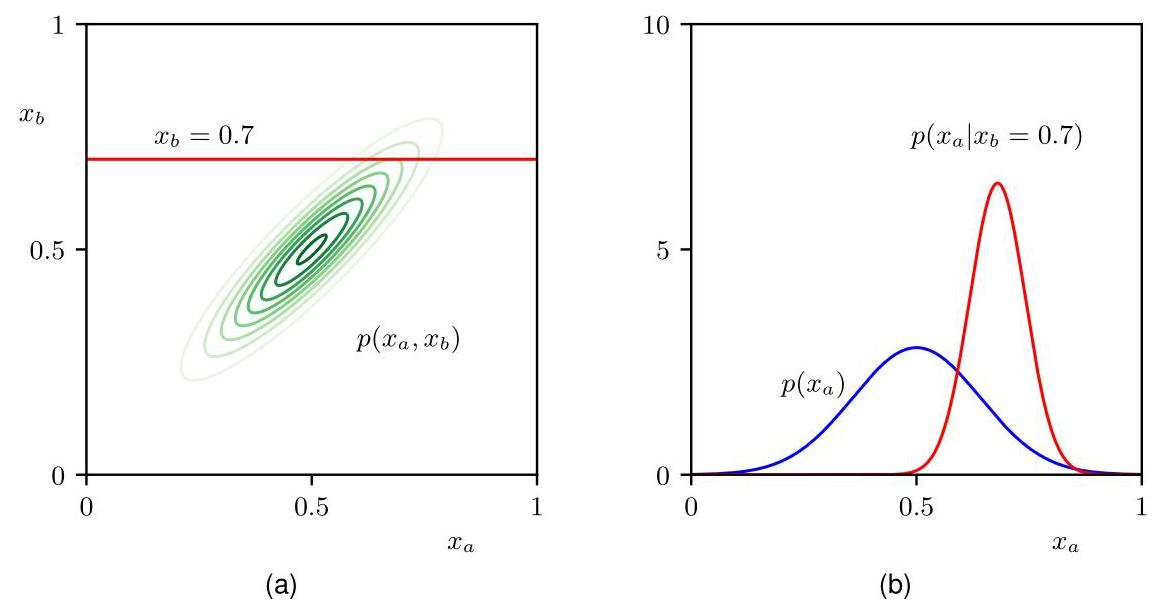
\includegraphics[max width=0.9\textwidth]{images/0194e279-9b28-703a-88f4-c3ac21e2010d_101_325_345_1158_609_0.jpg}
\end{center}
\hspace*{3em} 

图 3.5 (a) 两个变量上的高斯分布 \(p\left( {{x}_{a},{x}_{b}}\right)\) 的等高线。(b) 边缘分布 \(p\left( {x}_{a}\right)\) (蓝色曲线)和给定 \({x}_{b} = {0.7}\) 时的条件分布 \(p\left( {{x}_{a} \mid  {x}_{b}}\right)\) (红色曲线)。

首先,我们要找到 \(\mathbf{x}\) 和 \(\mathbf{y}\) 的联合分布的表达式。为此,我们

定义

\[
\mathbf{z} = \left( \begin{array}{l} \mathbf{x} \\  \mathbf{y} \end{array}\right)  \tag{3.85}
\]

然后考虑联合分布的对数:

\[
\ln p\left( \mathbf{z}\right)  = \ln p\left( \mathbf{x}\right)  + \ln p\left( {\mathbf{y} \mid  \mathbf{x}}\right)
\]

\[
=  - \frac{1}{2}{\left( \mathbf{x} - \mathbf{\mu }\right) }^{\mathrm{T}}\mathbf{\Lambda }\left( {\mathbf{x} - \mathbf{\mu }}\right)
\]

\[
- \frac{1}{2}{\left( \mathbf{y} - \mathbf{A}\mathbf{x} - \mathbf{b}\right) }^{\mathrm{T}}\mathbf{L}\left( {\mathbf{y} - \mathbf{A}\mathbf{x} - \mathbf{b}}\right)  + \text{ const } \tag{3.86}
\]

其中 ’const’ 表示与 \(\mathbf{x}\) 和 \(\mathbf{y}\) 无关的项。和之前一样,我们看到这是 \(\mathbf{z}\) 各分量的二次函数,因此, \(p\left( \mathbf{z}\right)\) 是高斯分布。为了求出这个高斯分布的精度,我们考虑 (3.86) 中的二阶项,它可以写成

\[
- \frac{1}{2}{\mathbf{x}}^{\mathrm{T}}\left( {\mathbf{\Lambda } + {\mathbf{A}}^{\mathrm{T}}\mathbf{{LA}}}\right) \mathbf{x} - \frac{1}{2}{\mathbf{y}}^{\mathrm{T}}\mathbf{{Ly}} + \frac{1}{2}{\mathbf{y}}^{\mathrm{T}}\mathbf{{LA}}\mathbf{x} + \frac{1}{2}{\mathbf{x}}^{\mathrm{T}}{\mathbf{A}}^{\mathrm{T}}\mathbf{{Ly}}
\]

\[
=  - \frac{1}{2}{\left( \begin{array}{l} \mathbf{x} \\  \mathbf{y} \end{array}\right) }^{\mathrm{T}}\left( \begin{matrix} \mathbf{\Lambda } + {\mathbf{A}}^{\mathrm{T}}\mathbf{{LA}} &  - {\mathbf{A}}^{\mathrm{T}}\mathbf{L} \\   - \mathbf{{LA}} & \mathbf{L} \end{matrix}\right) \left( \begin{array}{l} \mathbf{x} \\  \mathbf{y} \end{array}\right)  =  - \frac{1}{2}{\mathbf{z}}^{\mathrm{T}}\mathbf{R}\mathbf{z} \tag{3.87}
\]

因此,关于 \(\mathbf{z}\) 的高斯分布具有精度(协方差的逆)矩阵

由下式给出

\[
\mathbf{R} = \left( \begin{matrix} \mathbf{\Lambda } + {\mathbf{A}}^{\mathrm{T}}\mathbf{{LA}} &  - {\mathbf{A}}^{\mathrm{T}}\mathbf{L} \\   - \mathbf{{LA}} & \mathbf{L} \end{matrix}\right)  \tag{3.88}
\]

通过求精度矩阵的逆来得到协方差矩阵,这可以使用矩阵求逆公式 (3.60) 来完成,结果为

\[
\operatorname{cov}\left\lbrack  \mathbf{z}\right\rbrack   = {\mathbf{R}}^{-1} = \left( \begin{matrix} {\mathbf{\Lambda }}^{-1} & {\mathbf{\Lambda }}^{-1}{\mathbf{A}}^{\mathrm{T}} \\  \mathbf{A}{\mathbf{\Lambda }}^{-1} & {\mathbf{L}}^{-1} + \mathbf{A}{\mathbf{\Lambda }}^{-1}{\mathbf{A}}^{\mathrm{T}} \end{matrix}\right) . \tag{3.89}
\]

\HRule

练习 3.23

\HRule

类似地,我们可以通过确定 (3.86) 中的线性项来求出关于 \(\mathbf{z}\) 的高斯分布的均值,这些线性项由下式给出

\[
{\mathbf{x}}^{\mathrm{T}}\mathbf{\Lambda }\mathbf{\mu } - {\mathbf{x}}^{\mathrm{T}}{\mathbf{A}}^{\mathrm{T}}\mathbf{L}\mathbf{b} + {\mathbf{y}}^{\mathrm{T}}\mathbf{L}\mathbf{b} = {\left( \begin{array}{l} \mathbf{x} \\  \mathbf{y} \end{array}\right) }^{\mathrm{T}}\left( \begin{matrix} \mathbf{\Lambda }\mathbf{\mu } - {\mathbf{A}}^{\mathrm{T}}\mathbf{L}\mathbf{b} \\  \mathbf{L}\mathbf{b} \end{matrix}\right) . \tag{3.90}
\]

利用我们之前通过对多元高斯分布的二次型进行配方法得到的结果 (3.55),我们发现 \(\mathbf{z}\) 的均值由下式给出

\[
\mathbb{E}\left\lbrack  \mathbf{z}\right\rbrack   = {\mathbf{R}}^{-1}\left( \begin{matrix} \mathbf{\Lambda }\mathbf{\mu } - {\mathbf{A}}^{\mathrm{T}}\mathbf{L}\mathbf{b} \\  \mathbf{L}\mathbf{b} \end{matrix}\right) . \tag{3.91}
\]

\HRule

练习 3.24

\HRule

利用 (3.89),我们随后得到

\[
\mathbb{E}\left\lbrack  \mathbf{z}\right\rbrack   = \left( \begin{matrix} \mathbf{\mu } \\  \mathbf{A}\mathbf{\mu } + \mathbf{b} \end{matrix}\right) . \tag{3.92}
\]

接下来,我们要找到边缘分布 \(p\left( \mathbf{y}\right)\) 的表达式,其中我们对 \(\mathbf{x}\) 进行了边缘化处理。回顾一下,当用分块协方差矩阵表示时,高斯随机向量的部分分量的边缘分布具有特别简单的形式。具体来说,其均值和协方差分别由 (3.76) 和 (3.77) 给出。利用 (3.89) 和 (3.92),我们可以看到边缘分布 \(p\left( \mathbf{y}\right)\) 的均值和协方差由下式给出

\[
\mathbb{E}\left\lbrack  \mathbf{y}\right\rbrack   = \mathbf{A}\mathbf{\mu } + \mathbf{b} \tag{3.93}
\]

\[
\operatorname{cov}\left\lbrack  \mathbf{y}\right\rbrack   = {\mathbf{L}}^{-1} + \mathbf{A}{\mathbf{\Lambda }}^{-1}{\mathbf{A}}^{\mathrm{T}}. \tag{3.94}
\]

\HRule

第 3.2 节

\HRule

这个结果的一个特殊情况是当 \(\mathbf{A} = \mathbf{I}\) 时,在这种情况下,边缘分布简化为两个高斯分布的卷积,我们可以看到卷积的均值是两个高斯分布均值之和,卷积的协方差是它们协方差之和。

最后,我们寻求条件 \(p\left( {\mathbf{x} \mid  \mathbf{y}}\right)\) 的表达式。回想一下,条件分布的结果使用 (3.57) 和 (3.59) 以分块精度矩阵的形式最容易表达。将这些结果应用于 (3.89) 和 (3.92),我们发现条件分布 \(p\left( {\mathbf{x} \mid  \mathbf{y}}\right)\) 的均值和协方差由下式给出

\[
\mathbb{E}\left\lbrack  {\mathbf{x} \mid  \mathbf{y}}\right\rbrack   = {\left( \mathbf{\Lambda } + {\mathbf{A}}^{\mathrm{T}}\mathbf{{LA}}\right) }^{-1}\left\{  {{\mathbf{A}}^{\mathrm{T}}\mathbf{L}\left( {\mathbf{y} - \mathbf{b}}\right)  + \mathbf{\Lambda }\mathbf{\mu }}\right\}   \tag{3.95}
\]

\[
\operatorname{cov}\left\lbrack  {\mathbf{x} \mid  \mathbf{y}}\right\rbrack   = {\left( \mathbf{\Lambda } + {\mathbf{A}}^{\mathrm{T}}\mathbf{L}\mathbf{A}\right) }^{-1}. \tag{3.96}
\]

\HRule

3.2 节

\HRule

对这个条件分布的评估可以看作是贝叶斯定理的一个例子,其中我们将 \(p\left( \mathbf{x}\right)\) 解释为 \(\mathbf{x}\) 上的先验分布。如果变量 \(\mathbf{y}\) 被观测到,那么条件分布 \(p\left( {\mathbf{x} \mid  \mathbf{y}}\right)\) 表示 \(\mathbf{x}\) 上相应的后验分布。在找到了边缘分布和条件分布之后,我们实际上已经将联合分布 \(p\left( \mathbf{z}\right)  = p\left( \mathbf{x}\right) p\left( {\mathbf{y} \mid  \mathbf{x}}\right)\) 表示为 \(p\left( {\mathbf{x} \mid  \mathbf{y}}\right) p\left( \mathbf{y}\right)\) 的形式。

这些结果可以总结如下。给定 \(\mathrm{x}\) 的边缘高斯分布以及 \(\mathrm{x}\) 给定时 \(\mathrm{y}\) 的条件高斯分布,形式为

\[
p\left( \mathbf{x}\right)  = \mathcal{N}\left( {\mathbf{x} \mid  \mathbf{\mu },{\mathbf{\Lambda }}^{-1}}\right)  \tag{3.97}
\]

\[
p\left( {\mathbf{y} \mid  \mathbf{x}}\right)  = \mathcal{N}\left( {\mathbf{y} \mid  \mathbf{A}\mathbf{x} + \mathbf{b},{\mathbf{L}}^{-1}}\right) , \tag{3.98}
\]

那么 \(\mathbf{y}\) 的边缘分布以及 \(\mathbf{y}\) 给定时 \(\mathbf{x}\) 的条件分布由下式给出

\[
p\left( \mathbf{y}\right)  = \mathcal{N}\left( {\mathbf{y} \mid  \mathbf{{A\mu }} + \mathbf{b},{\mathbf{L}}^{-1} + {\mathbf{{A\Lambda }}}^{-1}{\mathbf{A}}^{\mathrm{T}}}\right)  \tag{3.99}
\]

\[
p\left( {\mathbf{x} \mid  \mathbf{y}}\right)  = \mathcal{N}\left( {\mathbf{x} \mid  \mathbf{\sum }\left\{  {{\mathbf{A}}^{\mathrm{T}}\mathbf{L}\left( {\mathbf{y} - \mathbf{b}}\right)  + \mathbf{\Lambda }\mathbf{\mu }}\right\}  ,\mathbf{\sum }}\right)  \tag{3.100}
\]

其中

\[
\mathbf{\sum } = {\left( \mathbf{\Lambda } + {\mathbf{A}}^{\mathrm{T}}\mathbf{{LA}}\right) }^{-1}. \tag{3.101}
\]

\section*{3.2.7 最大似然}

给定一个数据集 \(\mathbf{X} = {\left( {\mathbf{x}}_{1},\ldots ,{\mathbf{x}}_{N}\right) }^{\mathrm{T}}\) ,其中的观测值 \(\left\{  {\mathbf{x}}_{n}\right\}\) 假定是从多元高斯分布中独立抽取的,我们可以通过最大似然法来估计该分布的参数。对数似然函数由下式给出

\[
\ln p\left( {\mathbf{X} \mid  \mathbf{\mu },\mathbf{\sum }}\right)  =  - \frac{ND}{2}\ln \left( {2\pi }\right)  - \frac{N}{2}\ln \left| \mathbf{\sum }\right|  - \frac{1}{2}\mathop{\sum }\limits_{{n = 1}}^{N}{\left( {\mathbf{x}}_{n} - \mathbf{\mu }\right) }^{\mathrm{T}}{\mathbf{\sum }}^{-1}\left( {{\mathbf{x}}_{n} - \mathbf{\mu }}\right) . \tag{3.102}
\]

通过简单的重新排列,我们发现似然函数仅通过两个量依赖于数据集

\[
\mathop{\sum }\limits_{{n = 1}}^{N}{\mathbf{x}}_{n},\;\mathop{\sum }\limits_{{n = 1}}^{N}{\mathbf{x}}_{n}{\mathbf{x}}_{n}^{\mathrm{T}}. \tag{3.103}
\]

这些被称为高斯分布的充分统计量。利用 (A.19),对数似然关于 \(\mathbf{\mu }\) 的导数由下式给出

\[
\frac{\partial }{\partial \mathbf{\mu }}\ln p\left( {\mathbf{X} \mid  \mathbf{\mu },\mathbf{\sum }}\right)  = \mathop{\sum }\limits_{{n = 1}}^{N}{\mathbf{\sum }}^{-1}\left( {{\mathbf{x}}_{n} - \mathbf{\mu }}\right) , \tag{3.104}
\]

\HRule

附录 A

\HRule

令该导数为零,我们得到最大似然解

均值估计:

\[
{\mathbf{\mu }}_{\mathrm{{ML}}} = \frac{1}{N}\mathop{\sum }\limits_{{n = 1}}^{N}{\mathbf{x}}_{n} \tag{3.105}
\]

这是观测到的数据点集的均值。关于 \(\sum\) 对 (3.102) 进行最大化的过程要复杂得多。最简单的方法是忽略对称性约束,并证明得到的解满足所需的对称性。Magnus 和 Neudecker (1999) 中可以找到对该结果的其他推导方法,这些方法明确施加了对称性和正定性约束。结果如预期所示,形式为

\[
{\mathbf{\sum }}_{\mathrm{{ML}}} = \frac{1}{N}\mathop{\sum }\limits_{{n = 1}}^{N}\left( {{\mathbf{x}}_{n} - {\mathbf{\mu }}_{\mathrm{{ML}}}}\right) {\left( {\mathbf{x}}_{n} - {\mathbf{\mu }}_{\mathrm{{ML}}}\right) }^{\mathrm{T}}, \tag{3.106}
\]

\HRule

练习 3.28

\HRule

其中涉及 \({\mathbf{\mu }}_{\mathrm{{ML}}}\) ,因为这是关于 \(\mathbf{\mu }\) 和 \(\mathbf{\sum }\) 进行联合最大化的结果。注意, \({\mathbf{\mu }}_{\mathrm{{ML}}}\) 的解 (3.105) 不依赖于 \({\mathbf{\sum }}_{\mathrm{{ML}}}\) ,因此我们可以先计算 \({\mathbf{\mu }}_{\mathrm{{ML}}}\) ,然后用它来计算 \({\mathbf{\sum }}_{\mathrm{{ML}}}\) 。

如果我们在真实分布下计算最大似然解的期望,我们会得到以下结果

\[
\mathbb{E}\left\lbrack  {\mathbf{\mu }}_{\mathrm{{ML}}}\right\rbrack   = \mathbf{\mu } \tag{3.107}
\]

\[
\mathbb{E}\left\lbrack  {\mathbf{\sum }}_{\mathrm{{ML}}}\right\rbrack   = \frac{N - 1}{N}\mathbf{\sum }. \tag{3.108}
\]

\HRule

练习 3.29

\HRule

我们发现,均值的最大似然估计的期望等于真实均值。然而,协方差的最大似然估计的期望小于真实值,因此它是有偏的。我们可以通过定义一个不同的估计量 \(\widetilde{\mathbf{\sum }}\) 来纠正这种偏差,该估计量由下式给出

\[
\widetilde{\mathbf{\sum }} = \frac{1}{N - 1}\mathop{\sum }\limits_{{n = 1}}^{N}\left( {{\mathbf{x}}_{n} - {\mathbf{\mu }}_{\mathrm{{ML}}}}\right) {\left( {\mathbf{x}}_{n} - {\mathbf{\mu }}_{\mathrm{{ML}}}\right) }^{\mathrm{T}}. \tag{3.109}
\]

显然,从 (3.106) 和 (3.108) 可知, \(\widetilde{\mathbf{\sum }}\) 的期望等于 \(\mathbf{\sum }\) 。

\section*{3.2.8 序贯估计}

我们对最大似然解的讨论代表了一种批量方法,在这种方法中,会一次性考虑整个训练数据集。另一种选择是使用序贯方法,该方法允许逐个处理数据点,然后将其丢弃。对于在线应用以及当一次性对所有数据点进行批量处理不可行的大数据情况,这些方法非常重要。

考虑均值 \({\mathbf{\mu }}_{\mathrm{{ML}}}\) 的最大似然估计的结果 (3.105),当它基于 \(N\) 个观测值时,我们将其记为 \({\mathbf{\mu }}_{\mathrm{{ML}}}^{\left( N\right) }\) 。如果我们分离出最后一个数据点 \({\mathbf{x}}_{N}\) 的贡献,我们可以得到

\[
{\mathbf{\mu }}_{\mathrm{{ML}}}^{\left( N\right) } = \frac{1}{N}\mathop{\sum }\limits_{{n = 1}}^{N}{\mathbf{x}}_{n}
\]

\[
= \frac{1}{N}{\mathbf{x}}_{N} + \frac{1}{N}\mathop{\sum }\limits_{{n = 1}}^{{N - 1}}{\mathbf{x}}_{n}
\]

\[
= \frac{1}{N}{\mathbf{x}}_{N} + \frac{N - 1}{N}{\mathbf{\mu }}_{\mathrm{{ML}}}^{\left( N - 1\right) }
\]

\[
= {\mathbf{\mu }}_{\mathrm{{ML}}}^{\left( N - 1\right) } + \frac{1}{N}\left( {{\mathbf{x}}_{N} - {\mathbf{\mu }}_{\mathrm{{ML}}}^{\left( N - 1\right) }}\right) . \tag{3.110}
\]

\begin{center}
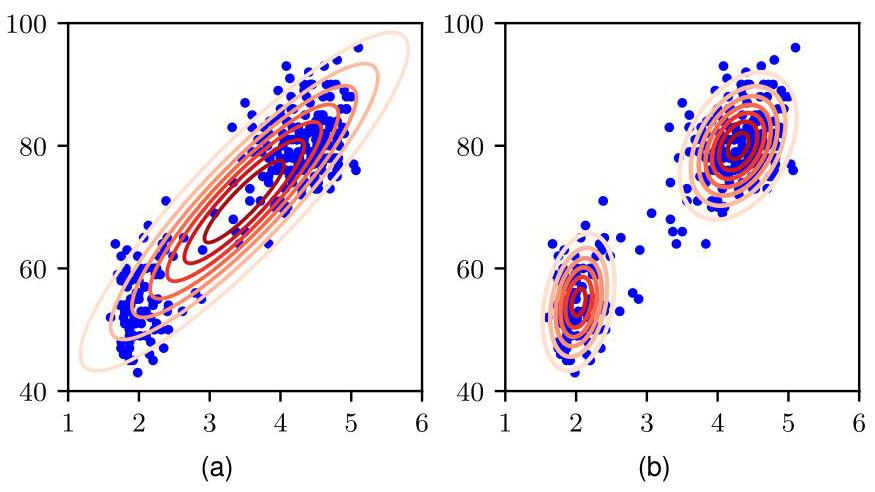
\includegraphics[max width=0.7\textwidth]{images/0194e279-9b28-703a-88f4-c3ac21e2010d_105_664_346_875_492_0.jpg}
\end{center}
\hspace*{3em} 

图 3.6 是老忠实间歇泉数据的绘图,其中红色曲线是等概率密度轮廓线。(a) 一个使用最大似然法拟合数据的单高斯分布。注意,这个分布未能捕捉到数据中的两个簇,实际上它将大部分概率质量置于簇之间的数据相对稀疏的中心区域。(b) 由两个高斯分布的线性组合给出的分布,同样使用最大似然法进行拟合,它能更好地表示数据。

这个结果有一个很好的解释,如下所述。在观察到 \(N - 1\) 个数据点后,我们用 \({\mathbf{\mu }}_{\mathrm{{ML}}}^{\left( N - 1\right) }\) 来估计 \(\mathbf{\mu }\) 。现在我们观察到数据点 \({\mathbf{x}}_{N}\) ,并通过将旧的估计值向 “误差信号” \(\left( {{\mathbf{x}}_{N} - {\mathbf{\mu }}_{\mathrm{{ML}}}^{\left( N - 1\right) }}\right)\) 的方向移动一小段距离(与 \(1/N\) 成比例)来得到修正后的估计值 \({\mathbf{\mu }}_{\mathrm{{ML}}}^{\left( N\right) }\) 。注意,随着 \(N\) 的增加,连续数据点的贡献会变小。

\section*{3.2.9 高斯混合模型}

尽管高斯分布具有一些重要的分析性质,但在用于对实际数据集进行建模时,它存在显著的局限性。考虑图 3.6(a) 所示的示例。这就是所谓的 “老忠实泉” 数据集,它包含了对美国黄石国家公园老忠实间歇泉喷发的 272 次测量数据。每次测量给出了喷发持续的分钟数(横轴)以及到下一次喷发的间隔分钟数(纵轴)。我们可以看到,该数据集形成了两个主要的簇,而简单的高斯分布无法捕捉到这种结构。

我们可能期望两个高斯分布的叠加能够更好地表示这个数据集中的结构,实际上

\begin{center}
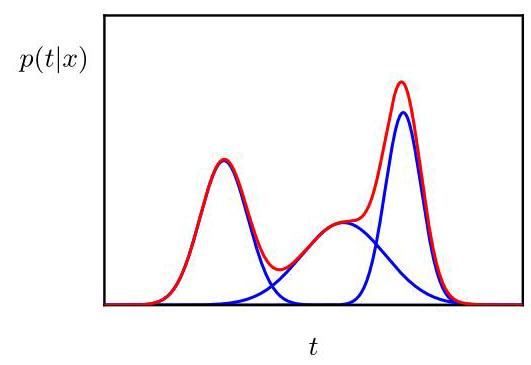
\includegraphics[max width=0.4\textwidth]{images/0194e279-9b28-703a-88f4-c3ac21e2010d_106_1020_344_531_365_0.jpg}
\end{center}
\hspace*{3em} 

图 3.7 一维高斯混合分布的示例,蓝色表示三个高斯分布(每个都乘以一个系数),红色表示它们的总和。

从图 3.6(b) 可以看出,情况确实如此。通过对更基本的分布(如高斯分布)进行线性组合而形成的这种叠加,可以被表述为称为混合分布的概率模型。在本节中,我们将以高斯分布为例来说明混合模型的框架。更一般地,混合模型可以包含其他分布的线性组合,例如用于二元变量的伯努利分布混合。在图 3.7 中,我们可以看到高斯分布的线性组合可以产生非常复杂的密度。通过使用足够数量的高斯分布,并调整它们的均值、协方差以及线性组合中的系数,几乎任何连续分布都可以以任意精度进行近似。

\HRule

第 15 章

\HRule

因此,我们考虑形式为 \(K\) 的高斯密度的叠加

\[
p\left( \mathbf{x}\right)  = \mathop{\sum }\limits_{{k = 1}}^{K}{\pi }_{k}\mathcal{N}\left( {\mathbf{x} \mid  {\mathbf{\mu }}_{k},{\mathbf{\sum }}_{k}}\right) , \tag{3.111}
\]

这被称为高斯混合模型。每个高斯密度 \(\mathcal{N}\left( {\mathbf{x} \mid  {\mathbf{\mu }}_{k},{\mathbf{\sum }}_{k}}\right)\) 都被称为混合模型的一个分量,并且有其自身的均值 \({\mathbf{\mu }}_{k}\) 和协方差 \({\mathbf{\sum }}_{k}\) 。具有三个分量的二维高斯混合模型的等高线图和曲面图如图 3.8 所示。

式 (3.111) 中的参数 \({\pi }_{k}\) 被称为混合系数。如果我们对式 (3.111) 两边关于 \(\mathbf{x}\) 进行积分,并注意到 \(p\left( \mathbf{x}\right)\) 和各个高斯分量都是归一化的,我们可以得到

\[
\mathop{\sum }\limits_{{k = 1}}^{K}{\pi }_{k} = 1 \tag{3.112}
\]

此外,已知 \(\mathcal{N}\left( {\mathbf{x} \mid  {\mathbf{\mu }}_{k},{\mathbf{\sum }}_{k}}\right)  \geq  0\) ,对于要求 \(p\left( \mathbf{x}\right)  \geq\) > 0 的一个充分条件是对于所有的 \(k\) 都有 \({\pi }_{k} \geq  0\) 。将此与条件 (3.112) 相结合,我们可以得到

\[
0 \leq  {\pi }_{k} \leq  1 \tag{3.113}
\]

因此,我们可以看到混合系数满足作为概率的要求,并且我们将证明混合分布的这种概率解释非常有用。

\HRule

第15章

\HRule

\begin{center}
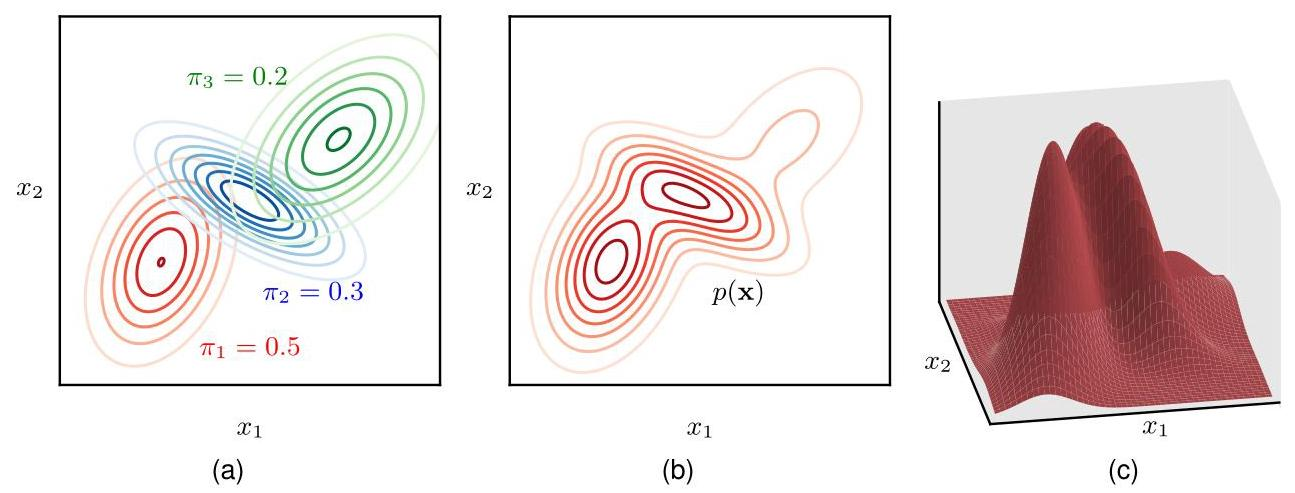
\includegraphics[max width=1.0\textwidth]{images/0194e279-9b28-703a-88f4-c3ac21e2010d_107_199_343_1295_493_0.jpg}
\end{center}
\hspace*{3em} 

图3.8 二维空间中三个高斯分布混合的示意图。(a) 每个混合分量的等密度轮廓,其中三个分量分别用红色、蓝色和绿色表示,每个分量下方显示了混合系数的值。(b) 混合分布的边缘概率密度 \(p\left( \mathbf{x}\right)\) 的轮廓。(c) 分布 \(p\left( \mathbf{x}\right)\) 的曲面图。

根据概率的求和规则和乘积规则,边缘密度可以写为

如下形式

\[
p\left( \mathbf{x}\right)  = \mathop{\sum }\limits_{{k = 1}}^{K}p\left( k\right) p\left( {\mathbf{x} \mid  k}\right) , \tag{3.114}
\]

这等价于式(3.111),其中我们可以将 \({\pi }_{k} = p\left( k\right)\) 视为选择第 \(k\) 个分量的先验概率,将密度 \(\mathcal{N}\left( {\mathbf{x} \mid  {\mathbf{\mu }}_{k},{\mathbf{\sum }}_{k}}\right)  = p\left( {\mathbf{x} \mid  k}\right)\) 视为在给定 \(k\) 的条件下 \(\mathbf{x}\) 的概率。正如我们将在后面的章节中看到的,相应的后验概率 \(p\left( {k \mid  \mathbf{x}}\right)\) 起着重要的作用,它们也被称为责任。根据贝叶斯定理,这些后验概率由下式给出

\[
{\gamma }_{k}\left( \mathbf{x}\right)  \equiv  p\left( {k \mid  \mathbf{x}}\right)
\]

\[
= \frac{p\left( k\right) p\left( {\mathbf{x} \mid  k}\right) }{\mathop{\sum }\limits_{l}p\left( l\right) p\left( {\mathbf{x} \mid  l}\right) }
\]

\[
= \frac{{\pi }_{k}\mathcal{N}\left( {\mathbf{x} \mid  {\mathbf{\mu }}_{k},{\mathbf{\sum }}_{k}}\right) }{\mathop{\sum }\limits_{l}{\pi }_{l}\mathcal{N}\left( {\mathbf{x} \mid  {\mathbf{\mu }}_{l},{\mathbf{\sum }}_{l}}\right) }. \tag{3.115}
\]

高斯混合分布的形式由参数 \(\pi\) 、 \(\mathbf{\mu }\) 和 \(\mathbf{\sum }\) 决定,这里我们使用了符号 \(\mathbf{\pi } \equiv  \left\{  {{\pi }_{1},\ldots ,{\pi }_{K}}\right\}  ,\mathbf{\mu } \equiv  \left\{  {{\mathbf{\mu }}_{1},\ldots ,{\mathbf{\mu }}_{K}}\right\}\) 和 \(\mathbf{\sum } \equiv  \left\{  {{\mathbf{\sum }}_{1},\ldots {\mathbf{\sum }}_{K}}\right\}\) 。设置这些参数值的一种方法是使用最大似然法。由式(3.111)可知,似然函数的对数为

\[
\ln p\left( {\mathbf{X} \mid  \mathbf{\pi },\mathbf{\mu },\mathbf{\sum }}\right)  = \mathop{\sum }\limits_{{n = 1}}^{N}\ln \left\{  {\mathop{\sum }\limits_{{k = 1}}^{K}{\pi }_{k}\mathcal{N}\left( {{\mathbf{x}}_{n} \mid  {\mathbf{\mu }}_{k},{\mathbf{\sum }}_{k}}\right) }\right\}   \tag{3.116}
\]

其中 \(\mathbf{X} = \left\{  {{\mathbf{x}}_{1},\ldots ,{\mathbf{x}}_{N}}\right\}\) 。我们立即可以看出,由于对数内部对 \(k\) 进行求和,现在的情况比单个高斯分布要复杂得多。因此,参数的最大似然解不再有封闭形式的解析解。最大化似然函数的一种方法是使用迭代数值优化技术。或者,我们可以采用一种强大的框架,称为期望最大化,它广泛适用于各种不同的深度生成模型。

\HRule

第15章

\HRule

\section*{3.3. 周期变量}

尽管高斯分布本身以及作为更复杂概率模型的构建块都具有重要的实际意义,但在某些情况下,它们并不适合作为连续变量的密度模型。在实际应用中出现的一个重要情况是周期变量。

周期变量的一个例子是特定地理位置的风向。例如,我们可能会在多个位置测量风向,并希望使用参数分布来总结这些数据。另一个例子是日历时间,我们可能对建模那些被认为在24小时或一年周期内具有周期性的量感兴趣。这些量可以方便地用角度(极坐标) \(0 \leq  \theta  < {2\pi }\) 来表示。

我们可能会想通过选择某个方向作为原点,然后应用诸如高斯分布这样的常规分布来处理周期变量。然而,这样的方法会得到强烈依赖于原点任意选择的结果。例如,假设我们在 \({\theta }_{1} = {1}^{ \circ  }\) 和 \({\theta }_{2} = {359}^{ \circ  }\) 处有两个观测值,并使用标准的单变量高斯分布对它们进行建模。如果我们将原点放在 \({0}^{ \circ  }\) 处,那么这个数据集的样本均值将是 \({180}^{ \circ  }\) ,标准差是 \({179}^{ \circ  }\) ;而如果我们将原点放在 \({180}^{ \circ  }\) 处,那么均值将是 \({0}^{ \circ  }\) ,标准差将是 \({1}^{ \circ  }\) 。显然,我们需要为周期变量开发一种特殊的方法。

\section*{3.3.1 冯·米塞斯分布}

让我们考虑评估一个周期变量 \(\theta\) 的一组观测值 \(\mathcal{D} = \left\{  {{\theta }_{1},\ldots ,{\theta }_{N}}\right\}\) 的均值的问题,其中 \(\theta\) 以弧度为单位进行测量。我们已经知道,简单平均值 \(\left( {{\theta }_{1} + \cdots  + {\theta }_{N}}\right) /N\) 将强烈依赖于坐标。为了找到均值的一个不变度量,注意到这些观测值可以被视为单位圆上的点,因此可以用二维单位向量 \({\mathbf{x}}_{1},\ldots ,{\mathbf{x}}_{N}\) 来描述,其中对于 \(n = 1,\ldots ,N\) 有 \(\begin{Vmatrix}{\mathbf{x}}_{n}\end{Vmatrix} = 1\) ,如图 3.9 所示。我们可以改为对向量 \(\left\{  {\mathbf{x}}_{n}\right\}\) 求平均,得到

\[
\overline{\mathbf{x}} = \frac{1}{N}\mathop{\sum }\limits_{{n = 1}}^{N}{\mathbf{x}}_{n} \tag{3.117}
\]

然后找到这个平均值对应的角度 \(\bar{\theta }\) 。显然,这个定义将确保均值的位置与角度坐标的原点无关。注意, \(\overline{\mathbf{x}}\) 通常会位于单位圆内部。笛卡尔坐标

\begin{center}
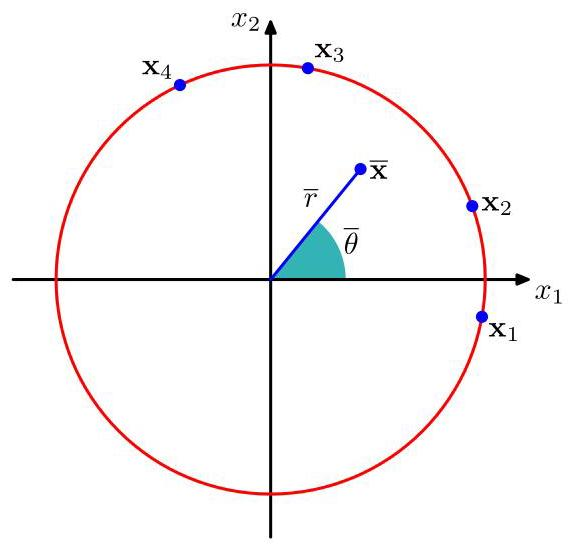
\includegraphics[max width=0.4\textwidth]{images/0194e279-9b28-703a-88f4-c3ac21e2010d_109_975_344_570_546_0.jpg}
\end{center}
\hspace*{3em} 

图 3.9 周期变量的值 \({\theta }_{n}\) 表示为位于单位圆上的二维向量 \({\mathbf{x}}_{n}\) 的图示。同时还展示了这些向量的平均值 \(\bar{x}\) 。

观测值的笛卡尔坐标由 \({\mathbf{x}}_{n} = \left( {\cos {\theta }_{n},\sin {\theta }_{n}}\right)\) 给出,我们可以将样本均值的笛卡尔坐标写成 \(\overline{\mathbf{x}} = \left( {\bar{r}\cos \bar{\theta },\bar{r}\sin \bar{\theta }}\right)\) 的形式。代入 (3.117) 式并使 \({x}_{1}\) 和 \({x}_{2}\) 分量相等,然后得到

\[
{\bar{x}}_{1} = \bar{r}\cos \bar{\theta } = \frac{1}{N}\mathop{\sum }\limits_{{n = 1}}^{N}\cos {\theta }_{n},\;{\bar{x}}_{2} = \bar{r}\sin \bar{\theta } = \frac{1}{N}\mathop{\sum }\limits_{{n = 1}}^{N}\sin {\theta }_{n}. \tag{3.118}
\]

取比值,并利用恒等式 \(\tan \theta  = \sin \theta /\cos \theta\) ,我们可以求解 \(\bar{\theta }\) 以

给予

\[
\bar{\theta } = {\tan }^{-1}\left\{  \frac{\mathop{\sum }\limits_{n}\sin {\theta }_{n}}{\mathop{\sum }\limits_{n}\cos {\theta }_{n}}\right\}  . \tag{3.119}
\]

很快,我们将看到这个结果是如何自然地作为最大似然估计量出现的。

首先,我们需要定义高斯分布的一种周期性推广,称为冯·米塞斯分布。在这里,我们将注意力限制在单变量分布上,尽管在任意维度的超球面上也可以找到类似的周期性分布(Mardia 和 Jupp,2000)。

按照惯例,我们将考虑周期为 \({2\pi }\) 的分布 \(p\left( \theta \right)\) 。任何在 \(\theta\) 上定义的概率密度 \(p\left( \theta \right)\) 不仅必须是非负的且积分值为 1,而且还必须是周期性的。因此, \(p\left( \theta \right)\) 必须满足三个条件:

\[
p\left( \theta \right)  \geq  0 \tag{3.120}
\]

\[
{\int }_{0}^{2\pi }p\left( \theta \right) \mathrm{d}\theta  = 1 \tag{3.121}
\]

\[
p\left( {\theta  + {2\pi }}\right)  = p\left( \theta \right) . \tag{3.122}
\]

由 (3.122) 可知,对于任意整数 \(M\) ,有 \(p\left( {\theta  + {M2\pi }}\right)  = p\left( \theta \right)\) 。

我们可以很容易地得到一个满足这三个性质的类似高斯分布,如下所示。考虑两个变量 \(\mathbf{x} = \left( {{x}_{1},{x}_{2}}\right)\) 的高斯分布,其均值为 \(\mathbf{\mu } = \left( {{\mu }_{1},{\mu }_{2}}\right)\) ,协方差矩阵为 \(\mathbf{\sum } = {\sigma }^{2}\mathbf{I}\) ,其中 \(\mathbf{I}\) 是 \(2 \times  2\) 单位矩阵,使得

\[
p\left( {{x}_{1},{x}_{2}}\right)  = \frac{1}{{2\pi }{\sigma }^{2}}\exp \left\{  {-\frac{{\left( {x}_{1} - {\mu }_{1}\right) }^{2} + {\left( {x}_{2} - {\mu }_{2}\right) }^{2}}{2{\sigma }^{2}}}\right\}  . \tag{3.123}
\]

\begin{center}
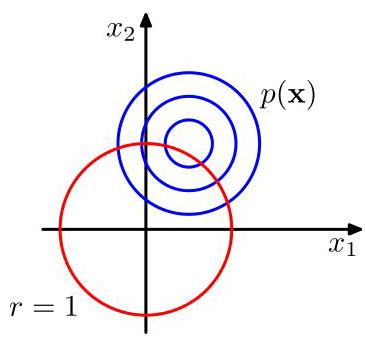
\includegraphics[max width=0.2\textwidth]{images/0194e279-9b28-703a-88f4-c3ac21e2010d_110_1177_344_365_339_0.jpg}
\end{center}
\hspace*{3em} 

图 3.10 冯·米塞斯分布可以通过考虑形式为 (3.123) 的二维高斯分布推导得出,其密度轮廓用蓝色表示,并以红色所示的单位圆为条件。

常数 \(p\left( \mathbf{x}\right)\) 的轮廓是圆形,如图 3.10 所示。

现在假设我们考虑这个分布在固定半径的圆上的值。那么根据构造,这个分布将是周期性的,尽管它不会被归一化。我们可以通过从笛卡尔坐标 \(\left( {{x}_{1},{x}_{2}}\right)\) 转换到极坐标 \(\left( {r,\theta }\right)\) 来确定这个分布的形式,使得

\[
{x}_{1} = r\cos \theta ,\;{x}_{2} = r\sin \theta . \tag{3.124}
\]

我们还通过写作将均值 \(\mathbf{\mu }\) 映射到极坐标中

\[
{\mu }_{1} = {r}_{0}\cos {\theta }_{0},\;{\mu }_{2} = {r}_{0}\sin {\theta }_{0}. \tag{3.125}
\]

接下来,我们将这些变换代入二维高斯分布 (3.123) 中,然后以单位圆 \(r = 1\) 为条件,注意我们只关注对 \(\theta\) 的依赖。关注高斯分布中的指数部分,我们有

\[
- \frac{1}{2{\sigma }^{2}}\left\{  {{\left( r\cos \theta  - {r}_{0}\cos {\theta }_{0}\right) }^{2} + {\left( r\sin \theta  - {r}_{0}\sin {\theta }_{0}\right) }^{2}}\right\}
\]

\[
=  - \frac{1}{2{\sigma }^{2}}\left\{  {1 + {r}_{0}^{2} - 2{r}_{0}\cos \theta \cos {\theta }_{0} - 2{r}_{0}\sin \theta \sin {\theta }_{0}}\right\}
\]

\[
= \frac{{r}_{0}}{{\sigma }^{2}}\cos \left( {\theta  - {\theta }_{0}}\right)  + \text{ const } \tag{3.126}
\]

其中 “const” 表示与 \(\theta\) 无关的项。我们使用了以下三角恒等式:

\[
{\cos }^{2}A + {\sin }^{2}A = 1 \tag{3.127}
\]

\[
\cos A\cos B + \sin A\sin B = \cos \left( {A - B}\right) . \tag{3.128}
\]

如果我们现在定义 \(m = {r}_{0}/{\sigma }^{2}\) ,我们将得到 \(p\left( \theta \right)\) 沿单位圆 \(r = 1\) 分布的最终表达式,其形式为

\[
p\left( {\theta  \mid  {\theta }_{0},m}\right)  = \frac{1}{{2\pi }{I}_{0}\left( m\right) }\exp \left\{  {m\cos \left( {\theta  - {\theta }_{0}}\right) }\right\}  , \tag{3.129}
\]

这被称为冯·米塞斯分布或圆形正态分布。这里的参数 \({\theta }_{0}\) 对应于分布的均值,而 \(m\) 被称为集中度参数,类似于高斯分布的逆方差(即精度)。(3.129) 中的归一化系数用 \({I}_{0}\left( m\right)\) 表示,它是第一类零阶修正贝塞尔函数(Abramowitz 和 Stegun,1965),定义为

\[
{I}_{0}\left( m\right)  = \frac{1}{2\pi }{\int }_{0}^{2\pi }\exp \{ m\cos \theta \} \mathrm{d}\theta . \tag{3.130}
\]

\begin{center}
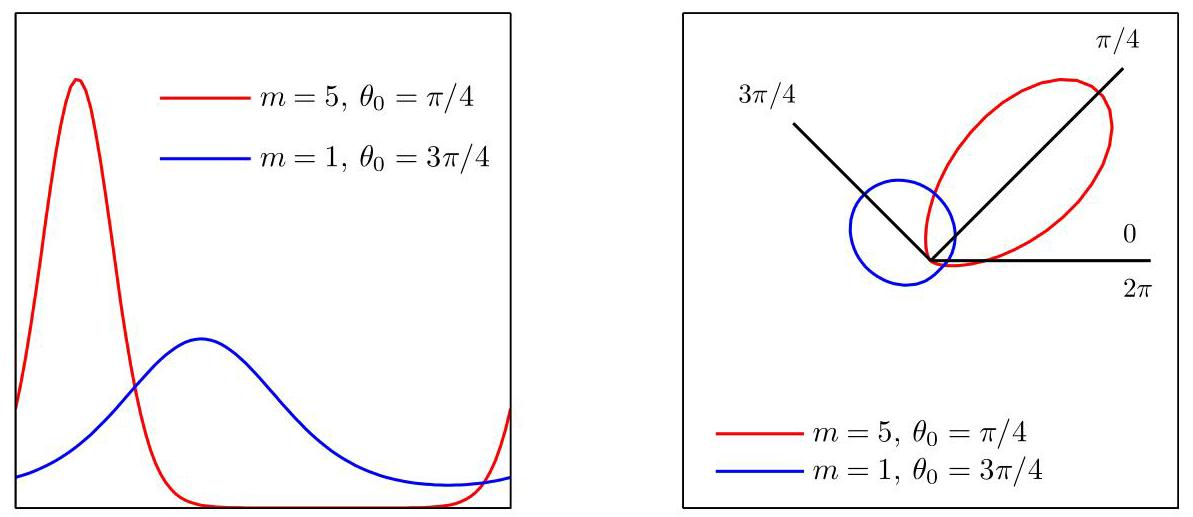
\includegraphics[max width=0.9\textwidth]{images/0194e279-9b28-703a-88f4-c3ac21e2010d_111_276_356_1193_517_0.jpg}
\end{center}
\hspace*{3em} 

图 3.11 绘制了两种不同参数值下的冯·米塞斯分布,左侧为直角坐标图,右侧为相应的极坐标图。

\HRule

练习 3.31

\HRule

对于较大的 \(m\) ,该分布近似为高斯分布。图 3.11 绘制了冯·米塞斯分布,图 3.12 绘制了函数 \({I}_{0}\left( m\right)\) 。

现在考虑冯·米塞斯分布参数 \({\theta }_{0}\) 和 \(m\) 的最大似然估计。对数似然函数由下式给出

\[
\ln p\left( {\mathcal{D} \mid  {\theta }_{0},m}\right)  =  - N\ln \left( {2\pi }\right)  - N\ln {I}_{0}\left( m\right)  + m\mathop{\sum }\limits_{{n = 1}}^{N}\cos \left( {{\theta }_{n} - {\theta }_{0}}\right) . \tag{3.131}
\]

令关于 \({\theta }_{0}\) 的导数等于零,可得

\[
\mathop{\sum }\limits_{{n = 1}}^{N}\sin \left( {{\theta }_{n} - {\theta }_{0}}\right)  = 0. \tag{3.132}
\]

为求解 \({\theta }_{0}\) ,我们利用三角恒等式

\[
\sin \left( {A - B}\right)  = \cos B\sin A - \cos A\sin B \tag{3.133}
\]

习题 3.32,由此我们得到

\[
{\theta }_{0}^{\mathrm{{ML}}} = {\tan }^{-1}\left\{  \frac{\mathop{\sum }\limits_{n}\sin {\theta }_{n}}{\mathop{\sum }\limits_{n}\cos {\theta }_{n}}\right\}  , \tag{3.134}
\]

\begin{center}
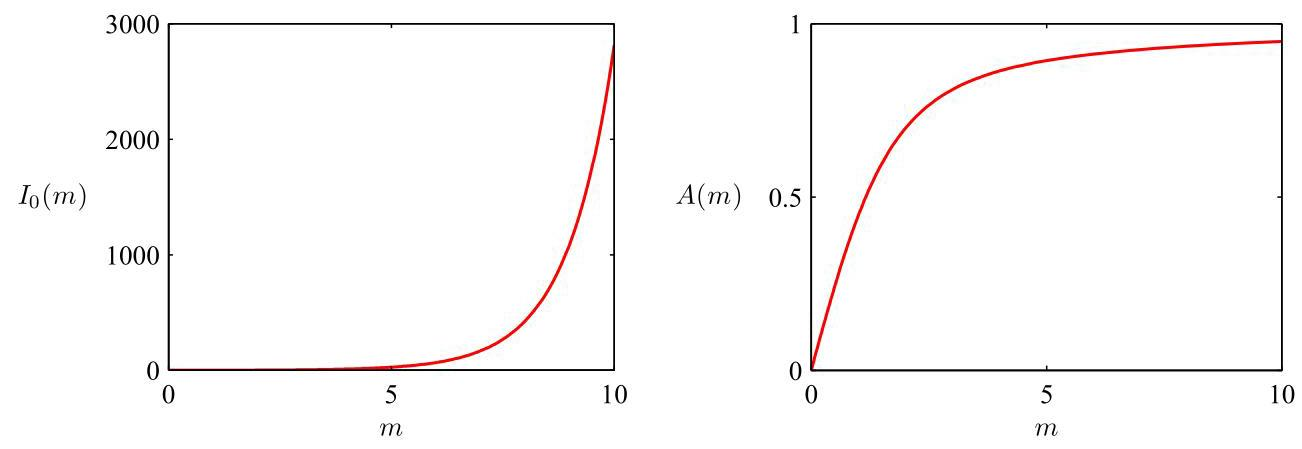
\includegraphics[max width=1.0\textwidth]{images/0194e279-9b28-703a-88f4-c3ac21e2010d_112_216_360_1302_449_0.jpg}
\end{center}
\hspace*{3em} 

图 3.12 由 (3.130) 定义的贝塞尔函数 \({I}_{0}\left( m\right)\) 以及由 (3.136) 定义的函数 \(A\left( m\right)\) 的图像。

我们认识到这就是之前在二维笛卡尔空间中观察值的均值所得到的结果 (3.119)。

类似地,关于 \(m\) 最大化 (3.131) 并利用 \({I}_{0}^{\prime }\left( m\right)  =\)  \({I}_{1}\left( m\right)\) (Abramowitz 和 Stegun,1965),我们有

\[
A\left( {m}_{\mathrm{{ML}}}\right)  = \frac{1}{N}\mathop{\sum }\limits_{{n = 1}}^{N}\cos \left( {{\theta }_{n} - {\theta }_{0}^{\mathrm{{ML}}}}\right)  \tag{3.135}
\]

其中我们代入了 \({\theta }_{0}^{\mathrm{{ML}}}\) 的最大似然解(回想一下,我们正在对 \(\theta\) 和 \(m\) 进行联合优化),并且我们定义了

\[
A\left( m\right)  = \frac{{I}_{1}\left( m\right) }{{I}_{0}\left( m\right) }. \tag{3.136}
\]

函数 \(A\left( m\right)\) 绘制在图 3.12 中。利用三角恒等式 (3.128),我们可以将 (3.135) 写成如下形式

\[
A\left( {m}_{\mathrm{{ML}}}\right)  = \left( {\frac{1}{N}\mathop{\sum }\limits_{{n = 1}}^{N}\cos {\theta }_{n}}\right) \cos {\theta }_{0}^{\mathrm{{ML}}} + \left( {\frac{1}{N}\mathop{\sum }\limits_{{n = 1}}^{N}\sin {\theta }_{n}}\right) \sin {\theta }_{0}^{\mathrm{{ML}}}. \tag{3.137}
\]

(3.137) 的右侧很容易计算,并且函数 \(A\left( m\right)\) 可以通过数值方法求逆。冯·米塞斯分布的一个局限性是它是单峰的。通过构建冯·米塞斯分布的混合模型,我们得到了一个灵活的框架,用于对可以处理多峰性的周期变量进行建模。

为了完整性,我们简要提及一些构建周期分布的替代技术。最简单的方法是使用观测值的直方图,其中角度坐标被划分为固定的区间。这具有

简单性和灵活性的优点,但也存在显著的局限性,正如我们稍后更详细讨论直方图方法时将看到的那样。另一种方法与冯·米塞斯分布类似,从欧几里得空间上的高斯分布开始,但现在是对单位圆进行边缘化而不是条件化(Mardia 和 Jupp,2000)。然而,这会导致更复杂的分布形式,我们将不再进一步讨论。最后,任何实轴上的有效分布(如高斯分布)都可以通过将宽度为 \({2\pi }\) 的连续区间映射到周期变量 \(\left( {0,{2\pi }}\right)\) 上转换为周期分布,这对应于将实轴“缠绕”在单位圆上。同样,得到的分布比冯·米塞斯分布更难处理。

\HRule

第 3.5 节

\HRule

\section*{3.4. 指数族}

我们在本章中到目前为止所研究的概率分布(混合模型除外)是一类广泛分布的具体示例,这类分布被称为指数族(Duda 和 Hart,1973 年;Bernardo 和 Smith,1994 年)。指数族的成员有许多重要的共同属性,一般性地讨论这些属性很有启发性。

给定参数 \(\mathbf{\eta }\) ,关于 \(\mathbf{x}\) 的指数族分布被定义为具有以下形式的分布集合

\[
p\left( {\mathbf{x} \mid  \mathbf{\eta }}\right)  = h\left( \mathbf{x}\right) g\left( \mathbf{\eta }\right) \exp \left\{  {{\mathbf{\eta }}^{\mathrm{T}}\mathbf{u}\left( \mathbf{x}\right) }\right\}   \tag{3.138}
\]

其中 \(\mathrm{x}\) 可以是标量或向量,并且可以是离散的或连续的。这里 \(\eta\) 被称为分布的自然参数, \(\mathbf{u}\left( \mathbf{x}\right)\) 是 \(\mathbf{x}\) 的某个函数。函数 \(g\left( \mathbf{\eta }\right)\) 可以被解释为确保分布归一化的系数,因此,它满足

\[
g\left( \mathbf{\eta }\right) \int h\left( \mathbf{x}\right) \exp \left\{  {{\mathbf{\eta }}^{\mathrm{T}}\mathbf{u}\left( \mathbf{x}\right) }\right\}  \mathrm{d}\mathbf{x} = 1 \tag{3.139}
\]

如果 \(\mathrm{x}\) 是离散变量,则积分替换为求和。

我们首先来看本章前面介绍的一些分布示例,并证明它们确实是指数族的成员。首先考虑伯努利分布:

\[
p\left( {x \mid  \mu }\right)  = \operatorname{Bern}\left( {x \mid  \mu }\right)  = {\mu }^{x}{\left( 1 - \mu \right) }^{1 - x}. \tag{3.140}
\]

将右侧表示为对数的指数形式,我们得到

\[
p\left( {x \mid  \mu }\right)  = \exp \{ x\ln \mu  + \left( {1 - x}\right) \ln \left( {1 - \mu }\right) \}
\]

\[
= \left( {1 - \mu }\right) \exp \left\{  {\ln \left( \frac{\mu }{1 - \mu }\right) x}\right\}  . \tag{3.141}
\]

与 (3.138) 进行比较,我们可以确定

\[
\eta  = \ln \left( \frac{\mu }{1 - \mu }\right)  \tag{3.142}
\]

我们可以对 \(\mu\) 求解,得到 \(\mu  = \sigma \left( \eta \right)\) ,其中

\[
\sigma \left( \eta \right)  = \frac{1}{1 + \exp \left( {-\eta }\right) } \tag{3.143}
\]

这被称为逻辑 sigmoid 函数。因此,我们可以使用标准表示 (3.138) 将伯努利分布写成如下形式

\[
p\left( {x \mid  \eta }\right)  = \sigma \left( {-\eta }\right) \exp \left( {\eta x}\right)  \tag{3.144}
\]

这里我们使用了 \(1 - \sigma \left( \eta \right)  = \sigma \left( {-\eta }\right)\) ,这可以从 (3.143) 轻松证明。与 (3.138) 比较可知

\[
u\left( x\right)  = x \tag{3.145}
\]

\[
h\left( x\right)  = 1 \tag{3.146}
\]

\[
g\left( \eta \right)  = \sigma \left( {-\eta }\right) . \tag{3.147}
\]

接下来考虑多项分布,对于单个观测值 \(\mathrm{x}\) ,

采用……形式

\[
p\left( {\mathbf{x} \mid  \mathbf{\mu }}\right)  = \mathop{\prod }\limits_{{k = 1}}^{M}{\mu }_{k}^{{x}_{k}} = \exp \left\{  {\mathop{\sum }\limits_{{k = 1}}^{M}{x}_{k}\ln {\mu }_{k}}\right\}   \tag{3.148}
\]

其中 \(\mathbf{x} = {\left( {x}_{1},\ldots ,{x}_{M}\right) }^{\mathrm{T}}\) 。同样,我们可以将其写成标准表示形式 (3.138),使得

\[
p\left( {\mathbf{x} \mid  \mathbf{\eta }}\right)  = \exp \left( {{\mathbf{\eta }}^{\mathrm{T}}\mathbf{x}}\right)  \tag{3.149}
\]

其中 \({\eta }_{k} = \ln {\mu }_{k}\) ,并且我们定义了 \(\mathbf{\eta } = {\left( {\eta }_{1},\ldots ,{\eta }_{M}\right) }^{\mathrm{T}}\) 。同样,与 (3.138) 比较,我们有

\[
\mathbf{u}\left( \mathbf{x}\right)  = \mathbf{x} \tag{3.150}
\]

\[
h\left( \mathbf{x}\right)  = 1 \tag{3.151}
\]

\[
g\left( \mathbf{\eta }\right)  = 1\text{ . } \tag{3.152}
\]

注意,参数 \({\eta }_{k}\) 不是相互独立的,因为参数 \({\mu }_{k}\) 受到约束条件的限制

\[
\mathop{\sum }\limits_{{k = 1}}^{M}{\mu }_{k} = 1 \tag{3.153}
\]

因此,给定参数 \({\mu }_{k}\) 中的任意 \(M - 1\) 个参数,其余参数的值就固定了。在某些情况下,通过仅用 \(M - 1\) 个参数来表示分布,消除这个约束会很方便。这可以通过使用关系 (3.153) 来实现,即根据其余的 \(\left\{  {\mu }_{k}\right\}\) (其中 \(k = 1,\ldots ,M - 1\) )来表示 \({\mu }_{M}\) ,从而消除 \({\mu }_{M}\) ,留下 \(M - 1\) 个参数。注意,这些剩余的参数仍然受到约束条件的限制

\[
0 \leq  {\mu }_{k} \leq  1,\;\mathop{\sum }\limits_{{k = 1}}^{{M - 1}}{\mu }_{k} \leq  1. \tag{3.154}
\]

利用约束条件 (3.153),这种表示形式下的多项分布就变为

\[
\exp \left\{  {\mathop{\sum }\limits_{{k = 1}}^{M}{x}_{k}\ln {\mu }_{k}}\right\}
\]

\[
= \exp \left\{  {\mathop{\sum }\limits_{{k = 1}}^{{M - 1}}{x}_{k}\ln {\mu }_{k} + \left( {1 - \mathop{\sum }\limits_{{k = 1}}^{{M - 1}}{x}_{k}}\right) \ln \left( {1 - \mathop{\sum }\limits_{{k = 1}}^{{M - 1}}{\mu }_{k}}\right) }\right\}
\]

\[
= \exp \left\{  {\mathop{\sum }\limits_{{k = 1}}^{{M - 1}}{x}_{k}\ln \left( \frac{{\mu }_{k}}{1 - \mathop{\sum }\limits_{{j = 1}}^{{M - 1}}{\mu }_{j}}\right)  + \ln \left( {1 - \mathop{\sum }\limits_{{k = 1}}^{{M - 1}}{\mu }_{k}}\right) }\right\}  . \tag{3.155}
\]

我们现在确定

\[
\ln \left( \frac{{\mu }_{k}}{1 - \mathop{\sum }\limits_{j}{\mu }_{j}}\right)  = {\eta }_{k}, \tag{3.156}
\]

我们可以通过以下步骤求解 \({\mu }_{k}\) :首先对 \(k\) 两边求和,然后重新整理并回代,得到

\[
{\mu }_{k} = \frac{\exp \left( {\eta }_{k}\right) }{1 + \mathop{\sum }\limits_{j}\exp \left( {\eta }_{j}\right) }. \tag{3.157}
\]

这被称为 softmax 函数或归一化指数函数。因此,在这种表示中,多项分布采用以下形式

\[
p\left( {\mathbf{x} \mid  \mathbf{\eta }}\right)  = {\left( 1 + \mathop{\sum }\limits_{{k = 1}}^{{M - 1}}\exp \left( {\eta }_{k}\right) \right) }^{-1}\exp \left( {{\mathbf{\eta }}^{\mathrm{T}}\mathbf{x}}\right) . \tag{3.158}
\]

这是指数族的标准形式,参数向量为 \(\mathbf{\eta } =\)  \({\left( {\eta }_{1},\ldots ,{\eta }_{M - 1}\right) }^{\mathrm{T}}\) ,其中

\[
\mathbf{u}\left( \mathbf{x}\right)  = \mathbf{x} \tag{3.159}
\]

\[
h\left( \mathbf{x}\right)  = 1 \tag{3.160}
\]

\[
g\left( \mathbf{\eta }\right)  = {\left( 1 + \mathop{\sum }\limits_{{k = 1}}^{{M - 1}}\exp \left( {\eta }_{k}\right) \right) }^{-1}. \tag{3.161}
\]

最后,让我们考虑高斯分布。对于单变量高斯分布,我们有

\[
p\left( {x \mid  \mu ,{\sigma }^{2}}\right)  = \frac{1}{{\left( 2\pi {\sigma }^{2}\right) }^{1/2}}\exp \left\{  {-\frac{1}{2{\sigma }^{2}}{\left( x - \mu \right) }^{2}}\right\}   \tag{3.162}
\]

\[
= \frac{1}{{\left( 2\pi {\sigma }^{2}\right) }^{1/2}}\exp \left\{  {-\frac{1}{2{\sigma }^{2}}{x}^{2} + \frac{\mu }{{\sigma }^{2}}x - \frac{1}{2{\sigma }^{2}}{\mu }^{2}}\right\}  , \tag{3.163}
\]

经过一些简单的整理后,它可以写成标准指数族形式 (3.138),其中

\[
\mathbf{\eta } = \left( \begin{matrix} \mu /{\sigma }^{2} \\   - 1/2{\sigma }^{2} \end{matrix}\right)  \tag{3.164}
\]

\[
\mathbf{u}\left( x\right)  = \left( \begin{matrix} x \\  {x}^{2} \end{matrix}\right)  \tag{3.165}
\]

\[
h\left( \mathbf{x}\right)  = {\left( 2\pi \right) }^{-1/2} \tag{3.166}
\]

\[
g\left( \mathbf{\eta }\right)  = {\left( -2{\eta }_{2}\right) }^{1/2}\exp \left( \frac{{\eta }_{1}^{2}}{4{\eta }_{2}}\right) . \tag{3.167}
\]

\HRule

练习 3.35

\HRule

最后,我们有时会使用 (3.138) 的一种受限形式,其中我们选择 \(\mathbf{u}\left( \mathbf{x}\right)  = \mathbf{x}\) 。然而,通过注意到如果 \(f\left( \mathbf{x}\right)\) 是一个归一化密度,那么

\[
\frac{1}{s}f\left( {\frac{1}{s}\mathbf{x}}\right)  \tag{3.168}
\]

也是一个归一化密度,其中 \(s > 0\) 是一个尺度参数。将这些结合起来,我们得到了一类形式受限的指数族类条件密度

\[
p\left( {\mathbf{x} \mid  {\mathbf{\lambda }}_{k},s}\right)  = \frac{1}{s}h\left( {\frac{1}{s}\mathbf{x}}\right) g\left( {\mathbf{\lambda }}_{k}\right) \exp \left\{  {\frac{1}{s}{\mathbf{\lambda }}_{k}^{\mathrm{T}}\mathbf{x}}\right\}  . \tag{3.169}
\]

注意,我们允许每个类别有其自己的参数向量 \({\mathbf{\lambda }}_{k}\) ,但我们假设这些类别共享相同的尺度参数 \(s\) 。

\section*{3.4.1 充分统计量}

现在让我们考虑使用最大似然技术来估计一般指数族分布 (3.138) 中的参数向量 \(\eta\) 的问题。对 (3.139) 两边关于 \(\mathbf{\eta }\) 取梯度,我们得到

\[
\nabla g\left( \mathbf{\eta }\right) \int h\left( \mathbf{x}\right) \exp \left\{  {{\mathbf{\eta }}^{\mathrm{T}}\mathbf{u}\left( \mathbf{x}\right) }\right\}  \mathrm{d}\mathbf{x}
\]

\[
+ g\left( \mathbf{\eta }\right) \int h\left( \mathbf{x}\right) \exp \left\{  {{\mathbf{\eta }}^{\mathrm{T}}\mathbf{u}\left( \mathbf{x}\right) }\right\}  \mathbf{u}\left( \mathbf{x}\right) \mathrm{d}\mathbf{x} = 0. \tag{3.170}
\]

重新整理并再次利用 (3.139) 式,可得

\[
- \frac{1}{g\left( \mathbf{\eta }\right) }\nabla g\left( \mathbf{\eta }\right)  = g\left( \mathbf{\eta }\right) \int h\left( \mathbf{x}\right) \exp \left\{  {{\mathbf{\eta }}^{\mathrm{T}}\mathbf{u}\left( \mathbf{x}\right) }\right\}  \mathbf{u}\left( \mathbf{x}\right) \mathrm{d}\mathbf{x} = \mathbb{E}\left\lbrack  {\mathbf{u}\left( \mathbf{x}\right) }\right\rbrack  . \tag{3.171}
\]

因此,我们得到如下结果

\[
- \nabla \ln g\left( \mathbf{\eta }\right)  = \mathbb{E}\left\lbrack  {\mathbf{u}\left( \mathbf{x}\right) }\right\rbrack  . \tag{3.172}
\]

注意, \(\mathbf{u}\left( \mathbf{x}\right)\) 的协方差可以用 \(g\left( \mathbf{\eta }\right)\) 的二阶导数来表示,高阶矩的情况类似。因此,只要我们能对指数族分布进行归一化,就总能通过简单的求导得到它的矩。

\HRule

练习 3.36

\HRule

现在考虑一组独立同分布的数据,用 \(\mathbf{X} =\)  \(\left\{  {{\mathbf{x}}_{1},\ldots ,{\mathbf{x}}_{n}}\right\}\) 表示,其似然函数为

\[
p\left( {\mathbf{X} \mid  \mathbf{\eta }}\right)  = \left( {\mathop{\prod }\limits_{{n = 1}}^{N}h\left( {\mathbf{x}}_{n}\right) }\right) g{\left( \mathbf{\eta }\right) }^{N}\exp \left\{  {{\mathbf{\eta }}^{\mathrm{T}}\mathop{\sum }\limits_{{n = 1}}^{N}\mathbf{u}\left( {\mathbf{x}}_{n}\right) }\right\}  . \tag{3.173}
\]

令 \(\ln p\left( {\mathbf{X} \mid  \mathbf{\eta }}\right)\) 关于 \(\mathbf{\eta }\) 的梯度为零,我们得到最大似然估计量 \({\mathbf{\eta }}_{\mathrm{{ML}}}\) 需满足以下条件:

\[
- \nabla \ln g\left( {\mathbf{\eta }}_{\mathrm{{ML}}}\right)  = \frac{1}{N}\mathop{\sum }\limits_{{n = 1}}^{N}\mathbf{u}\left( {\mathbf{x}}_{n}\right) , \tag{3.174}
\]

原则上可以求解该式以得到 \({\eta }_{\mathrm{{ML}}}\) 。我们看到,最大似然估计量的解仅通过 \(\mathop{\sum }\limits_{n}\mathbf{u}\left( {\mathbf{x}}_{n}\right)\) 依赖于数据,因此 \(\mathop{\sum }\limits_{n}\mathbf{u}\left( {\mathbf{x}}_{n}\right)\) 被称为分布 (3.138) 的充分统计量。我们不需要存储整个数据集本身,而只需要存储充分统计量的值。例如,对于伯努利分布,函数 \(\mathbf{u}\left( x\right)\) 由 \(x\) 给出,因此我们只需要保留数据点 \(\left\{  {x}_{n}\right\}\) 的总和;而对于高斯分布 \(\mathbf{u}\left( x\right)  = {\left( x,{x}^{2}\right) }^{\mathrm{T}}\) ,因此我们应该同时保留 \(\left\{  {x}_{n}\right\}\) 的总和以及 \(\left\{  {x}_{n}^{2}\right\}\) 的总和。

如果我们考虑极限 \(N \rightarrow  \infty\) ,那么 (3.174) 式的右侧变为 \(\mathbb{E}\left\lbrack  {\mathbf{u}\left( \mathbf{x}\right) }\right\rbrack\) ,因此通过与 (3.172) 式比较,我们发现在这个极限下, \({\mathbf{\eta }}_{\mathrm{{ML}}}\) 将等于真实值 \(\eta\) 。

\section*{3.5. 非参数方法}

在本章中,我们一直专注于使用具有特定函数形式的概率分布,这些分布由少量参数控制,其值需要从数据集中确定。这被称为密度建模的参数化方法。这种方法的一个重要局限性在于,所选择的密度可能无法很好地拟合生成数据的分布,从而导致较差的预测性能。例如,如果生成数据的过程是多峰的,那么高斯分布(必然是单峰的)永远无法捕捉到分布的这一特征。在最后这一节中,我们将考虑一些非参数密度估计方法,这些方法对分布的形式所做的假设较少。

\section*{3.5.1 直方图}

让我们从讨论用于密度估计的直方图方法开始,我们已经在图 2.5 中关于边缘分布和条件分布的内容以及图 3.2 中关于中心极限定理的内容中遇到过这种方法。在这里,我们将更详细地探讨直方图密度模型的性质,重点关注具有单个连续变量 \(x\) 的情况。标准直方图只是将 \(x\) 划分为宽度为 \({\Delta }_{i}\) 的不同区间,然后统计落入

\begin{center}
\includegraphics[max width=0.4\textwidth]{images/0194e279-9b28-703a-88f4-c3ac21e2010d_118_942_368_548_453_0.jpg}
\end{center}
\hspace*{3em} 

图 3.13 展示了使用直方图方法进行密度估计的示例,其中 50 个数据点的数据集是从绿色曲线所示的分布中生成的。图中展示了基于公式 (3.175)、使用不同的公共区间宽度 \(\Delta\) 得到的直方图密度估计。

在区间 \(i\) 内。为了将这个计数转换为归一化的概率密度,我们只需将其除以观测值的总数 \(N\) 以及区间的宽度 \({\Delta }_{i}\) ,从而得到每个区间的概率值:

\[
{p}_{i} = \frac{{n}_{i}}{N{\Delta }_{i}} \tag{3.175}
\]

对于该式,很容易看出 \(\int p\left( x\right) \mathrm{d}x = 1\) 。这给出了一个密度 \(p\left( x\right)\) 的模型,该模型在每个区间的宽度上是恒定的。通常,区间会被选择为具有相同的宽度 \({\Delta }_{i} = \Delta\) 。

在图 3.13 中,我们展示了一个直方图密度估计的示例。这里的数据是从对应于绿色曲线的分布中抽取的,该曲线由两个高斯分布混合而成。图中还展示了对应于区间宽度 \(\Delta\) 的三种不同选择的直方图密度估计示例。我们看到,当 \(\Delta\) 非常小时(上图),得到的密度模型非常尖锐,具有很多在生成数据集的底层分布中不存在的结构。相反,如果 \(\Delta\) 太大(下图),则结果是一个过于平滑的模型,因此无法捕捉到绿色曲线的双峰特性。对于 \(\Delta\) 的某个中间值(中图),可以得到最佳结果。原则上,直方图密度模型也依赖于区间边缘位置的选择,不过这通常远不如区间宽度 \(\Delta\) 重要。

请注意,直方图方法具有这样的特性(与稍后要讨论的方法不同):一旦计算出直方图,数据集本身就可以被丢弃,如果数据集很大,这可能是一个优势。此外,如果数据点是依次到达的,直方图方法也很容易应用。

在实践中,直方图技术可用于快速可视化一维或二维数据,但不适合大多数密度估计应用。一个明显的问题是,估计的密度存在不连续性,这是由于区间边缘造成的,而不是生成数据的底层分布的任何特性。直方图方法的一个主要局限性是其随维度的缩放问题。如果我们将 \(D\) 维空间中的每个变量划分为 \(M\) 个区间,那么区间的总数将是 \({M}^{D}\) 。这种随 \(D\) 的指数缩放是维度灾难的一个例子。在高维空间中,为了对局部概率密度提供有意义的估计所需的数据量将是巨大的。

\HRule

6.1.1 节

\HRule

然而,直方图方法用于密度估计给我们上了重要的两课。首先,为了估计特定位置的概率密度,我们应该考虑位于该点某个局部邻域内的数据点。请注意,局部性的概念要求我们假设某种形式的距离度量,在这里我们一直假设使用欧几里得距离。对于直方图,这种邻域属性由区间定义,并且有一个自然的“平滑”参数来描述局部区域的空间范围,在这种情况下就是区间宽度。其次,为了获得良好的结果,平滑参数的值既不应太大也不应太小。这让人想起多项式回归中模型复杂度的选择,其中多项式的次数 \(M\) ,或者正则化参数的值 \(\lambda\) ,在某个中间值时是最优的,既不过大也不过小。有了这些见解,我们现在转向讨论两种广泛使用的非参数密度估计技术,核估计器和最近邻方法,它们在维度上的扩展性比简单的直方图模型更好。

\HRule

第 1 章

\HRule

\section*{3.5.2 核密度}

让我们假设观测值是从某个 \(D\) 维空间中的某个未知概率密度 \(p\left( \mathbf{x}\right)\) 中抽取的,我们将该空间视为欧几里得空间,并且我们希望估计 \(p\left( \mathbf{x}\right)\) 的值。根据我们之前对局部性的讨论,让我们考虑包含 \(\mathbf{x}\) 的某个小区域 \(\mathcal{R}\) 。与该区域相关的概率质量由下式给出

\[
P = {\int }_{\mathcal{R}}p\left( \mathbf{x}\right) \mathrm{d}\mathbf{x}. \tag{3.176}
\]

现在假设我们已经收集了一个数据集,其中包含从 \(p\left( \mathbf{x}\right)\) 中抽取的 \(N\) 个观测值。因为每个数据点落入 \(\mathcal{R}\) 的概率为 \(P\) ,所以位于 \(\mathcal{R}\) 内的点的总数 \(K\) 将服从二项分布

\HRule

第3.1.2节

\HRule

分布:

\[
\operatorname{Bin}\left( {K \mid  N,P}\right)  = \frac{N!}{K!\left( {N - K}\right) !}{P}^{K}{\left( 1 - P\right) }^{N - K}. \tag{3.177}
\]

使用(3.11),我们发现落在该区域内的点的平均比例为 \(\mathbb{E}\left\lbrack  {K/N}\right\rbrack   = P\) ,同样,使用(3.12),我们发现围绕该平均值的方差为 \(\operatorname{var}\left\lbrack  {K/N}\right\rbrack   = P\left( {1 - P}\right) /N\) 。对于较大的 \(N\) ,这种分布将在平均值附近出现尖锐的峰值,因此

\[
K \simeq  {NP}. \tag{3.178}
\]

然而,如果我们还假设区域 \(\mathcal{R}\) 足够小,使得概率密度 \(p\left( \mathbf{x}\right)\) 在该区域内大致恒定,那么我们有

\[
P \simeq  p\left( \mathbf{x}\right) V \tag{3.179}
\]

其中 \(V\) 是 \(\mathcal{R}\) 的体积。结合(3.178)和(3.179),我们得到密度

估计形式为

\[
p\left( \mathbf{x}\right)  = \frac{K}{NV}. \tag{3.180}
\]

请注意,(3.180) 的有效性依赖于两个相互矛盾的假设,即区域 \(\mathcal{R}\) 足够小,使得该区域内的密度近似恒定,但又足够大(相对于该密度值而言),使得落在该区域内的点的数量 \(K\) 足以让二项分布呈现尖锐的峰值。

我们可以通过两种不同的方式利用结果 (3.180)。要么我们固定 \(K\) 并从数据中确定 \(V\) 的值,这就产生了稍后要讨论的 \(K\) -最近邻技术;要么我们固定 \(V\) 并从数据中确定 \(K\) ,这就产生了核方法。可以证明,只要 \(V\) 随 \(N\) 缩小,并且 \(K\) 随 \(N\) 以适当的速率增长(Duda 和 Hart,1973), \(K\) -最近邻密度估计器和核密度估计器在极限 \(N \rightarrow  \infty\) 下都会收敛到真实的概率密度。

我们首先详细讨论核方法。首先,我们将区域 \(\mathcal{R}\) 取为一个以点 \(\mathbf{x}\) 为中心的小超立方体,我们希望在该点确定概率密度。为了计算落在该区域内的点的数量 \(K\) ,方便起见,我们定义以下函数:

\[
k\left( \mathbf{u}\right)  = \left\{  {\begin{array}{ll} 1, & \left| {u}_{i}\right|  \leq  1/2, \\  0, & \text{ otherwise, } \end{array}\;i = 1,\ldots ,D,}\right.  \tag{3.181}
\]

它表示一个以原点为中心的单位立方体。函数 \(k\left( \mathbf{u}\right)\) 是核函数的一个例子,在这种情况下,它也被称为 Parzen 窗。根据 (3.181),如果数据点 \({\mathbf{x}}_{n}\) 位于以 \(\mathbf{x}\) 为中心、边长为 \(h\) 的立方体内,则量 \(k\left( {\left( {\mathbf{x} - {\mathbf{x}}_{n}}\right) /h}\right)\) 为 1,否则为 0。因此,位于这个立方体内的数据点的总数将是

\[
K = \mathop{\sum }\limits_{{n = 1}}^{N}k\left( \frac{\mathbf{x} - {\mathbf{x}}_{n}}{h}\right) . \tag{3.182}
\]

然后将这个表达式代入 (3.180),就得到了在 \(\mathbf{x}\) 处估计密度的以下结果:

\[
p\left( \mathbf{x}\right)  = \frac{1}{N}\mathop{\sum }\limits_{{n = 1}}^{N}\frac{1}{{h}^{D}}k\left( \frac{\mathbf{x} - {\mathbf{x}}_{n}}{h}\right)  \tag{3.183}
\]

其中我们用 \(V = {h}^{D}\) 表示 \(D\) 维中边长为 \(h\) 的超立方体的体积。利用函数 \(k\left( \mathbf{u}\right)\) 的对称性,我们现在可以重新解释这个方程,不是将其看作是以 \(\mathbf{x}\) 为中心的单个立方体,而是看作是以 \(N\) 个数据点 \({\mathbf{x}}_{n}\) 为中心的 \(N\) 个立方体的总和。

就目前情况而言,核密度估计器(3.183)会遇到与直方图方法相同的问题之一,即存在人为的不连续性,在这种情况下是在立方体的边界处。如果我们选择一个更平滑的核函数,就可以得到一个更平滑的密度模型,常见的选择是高斯核函数,这就产生了以下核密度模型:

\[
p\left( \mathbf{x}\right)  = \frac{1}{N}\mathop{\sum }\limits_{{n = 1}}^{N}\frac{1}{{\left( 2\pi {h}^{2}\right) }^{D/2}}\exp \left\{  {-\frac{{\begin{Vmatrix}\mathbf{x} - {\mathbf{x}}_{n}\end{Vmatrix}}^{2}}{2{h}^{2}}}\right\}   \tag{3.184}
\]

\begin{center}
\includegraphics[max width=0.4\textwidth]{images/0194e279-9b28-703a-88f4-c3ac21e2010d_121_942_368_551_454_0.jpg}
\end{center}
\hspace*{3em} 

图3.14展示了将核密度模型(3.184)应用于与图3.13中用于演示直方图方法相同的数据集的情况。我们看到 \(h\) 起到了平滑参数的作用,如果将其设置得太小(上图),结果会是一个噪声很大的密度模型;而如果将其设置得太大(下图),则生成数据的底层分布的双峰性质(由绿色曲线表示)就会被抹平。对于 \(h\) 的某个中间值(中图),可以得到最佳的密度模型。

其中 \(h\) 表示高斯分量的标准差。因此,我们的密度模型是通过在每个数据点上放置一个高斯分布,将整个数据集上的贡献相加,然后除以 \(N\) 以使密度得到正确归一化而得到的。在图3.14中,我们将模型(3.184)应用于前面用于演示直方图技术的数据集。正如预期的那样,我们看到参数 \(h\) 起到了平滑参数的作用,并且在 \(h\) 较小时对噪声的敏感性和 \(h\) 较大时的过度平滑之间存在权衡。同样, \(h\) 的优化是一个模型复杂度问题,类似于直方图密度估计中箱宽度的选择或曲线拟合中所用多项式的次数的选择。

我们可以在(3.183)中选择任何其他满足以下条件的核函数 \(k\left( \mathbf{u}\right)\)

\[
k\left( \mathbf{u}\right)  \geq  0, \tag{3.185}
\]

\[
\int k\left( \mathbf{u}\right) \mathrm{d}\mathbf{u} = 1 \tag{3.186}
\]

这些条件确保得到的概率分布在任何地方都是非负的,并且积分结果为1。由(3.183)给出的这类密度模型称为核密度估计器或帕曾估计器。它有一个很大的优点,即在“训练”阶段不需要进行计算,因为这只需要存储训练集。然而,这也是它的一个很大的缺点,因为评估密度的计算成本会随着数据集的大小线性增长。

\begin{center}
\includegraphics[max width=0.4\textwidth]{images/0194e279-9b28-703a-88f4-c3ac21e2010d_122_940_369_552_454_0.jpg}
\end{center}
\hspace*{3em} 

图3.15展示了使用与图3.14和图3.13中相同的数据集进行 \(K\) -最近邻密度估计的情况。我们看到参数 \(K\) 控制着平滑程度,因此 \(K\) 的值较小时会导致一个噪声很大的密度模型(上图),而 \(K\) 的值较大时(下图)会抹平生成数据集的真实分布的双峰性质(由绿色曲线表示)。

\section*{3.5.3 最近邻}

核方法进行密度估计的困难之一在于,控制核宽度的参数 \(h\) 对于所有核都是固定的。在数据密度高的区域, \(h\) 的较大值可能导致过度平滑,从而抹去原本可以从数据中提取的结构信息。然而,减小 \(h\) 可能会在数据空间中密度较小的其他地方导致估计结果出现噪声。因此, \(h\) 的最优选择可能取决于数据空间中的位置。最近邻方法用于密度估计可以解决这个问题。

因此,我们回到局部密度估计的一般结果 (3.180),不再固定 \(V\) 并从数据中确定 \(K\) 的值,而是考虑固定 \(K\) 的值,并利用数据为 \(V\) 找到合适的值。为此,我们考虑一个以点 \(\mathbf{x}\) 为中心的小球体,我们希望在该点估计密度 \(p\left( \mathbf{x}\right)\) ,并让球体的半径不断增大,直到它恰好包含 \(K\) 个数据点。然后,将 \(V\) 设置为所得球体的体积,通过 (3.180) 式给出密度 \(p\left( \mathbf{x}\right)\) 的估计值。这种技术称为 \(K\) 最近邻,图 3.15 展示了使用与图 3.13 和 3.14 相同的数据集,对参数 \(K\) 进行不同选择时的情况。我们看到, \(K\) 的值现在控制着平滑程度,并且同样存在一个既不太大也不太小的 \(K\) 最优选择。请注意, \(K\) 最近邻产生的模型不是一个真正的密度模型,因为在整个空间上的积分是发散的。

\HRule

练习 3.38

\HRule

在本章结尾,我们将展示如何将用于密度估计的 \(K\) -最近邻技术扩展到分类问题。为此,我们分别对每个类别应用 \(K\) -最近邻密度估计技术,然后利用贝叶斯定理。假设我们有一个数据集,其中类别 \({\mathcal{C}}_{k}\) 包含 \({N}_{k}\) 个点,总共有 \(N\) 个点,即 \(\mathop{\sum }\limits_{k}{N}_{k} = N\) 。如果我们希望对一个新点 \(\mathbf{x}\) 进行分类,我们以 \(\mathbf{x}\) 为中心绘制一个球体,使其恰好包含 \(K\) 个点,而不考虑这些点所属的类别。假设这个球体的体积为 \(V\) ,并且包含来自类别 \({\mathcal{C}}_{k}\) 的 \({K}_{k}\) 个点。那么 (3.180) 式提供了与之相关的密度估计

\begin{center}
\includegraphics[max width=0.7\textwidth]{images/0194e279-9b28-703a-88f4-c3ac21e2010d_123_654_342_888_480_0.jpg}
\end{center}
\hspace*{3em} 

图 3.16 (a) 在 \(K\) -最近邻分类器中,一个新点(用黑色菱形表示)根据 \(K\) 个最近训练数据点的多数类别成员身份进行分类,在这种情况下 \(K =\) = 3。(b) 在最近邻 \(\left( {K = 1}\right)\) 分类方法中,得到的决策边界由超平面组成,这些超平面是不同类别点对的垂直平分线。

对于每个类别:

\[
p\left( {\mathbf{x} \mid  {\mathcal{C}}_{k}}\right)  = \frac{{K}_{k}}{{N}_{k}V}. \tag{3.187}
\]

类似地,无条件密度由下式给出

\[
p\left( \mathbf{x}\right)  = \frac{K}{NV} \tag{3.188}
\]

并且类别先验由下式给出

\[
p\left( {\mathcal{C}}_{k}\right)  = \frac{{N}_{k}}{N}. \tag{3.189}
\]

现在,我们可以使用贝叶斯定理将 (3.187)、(3.188) 和 (3.189) 结合起来,以获得类别归属的后验概率:

\[
p\left( {{\mathcal{C}}_{k} \mid  \mathbf{x}}\right)  = \frac{p\left( {\mathbf{x} \mid  {\mathcal{C}}_{k}}\right) p\left( {\mathcal{C}}_{k}\right) }{p\left( \mathbf{x}\right) } = \frac{{K}_{k}}{K}. \tag{3.190}
\]

我们可以通过将测试点 \(\mathrm{x}\) 分配给后验概率最大的类别来最小化分类错误的概率,该类别对应于 \({K}_{k}/K\) 的最大值。因此,为了对一个新点进行分类,我们从训练数据集中找出 \(K\) 个最近的点,然后将新点分配给在这个集合中代表数量最多的类别。若出现平局,可以随机打破。 \(K = 1\) 的特殊情况称为最近邻规则,因为测试点简单地被分配到与训练集中最近点相同的类别。这些概念如图 3.16 所示。

最近邻 \(\left( {K = 1}\right)\) 分类器的一个有趣性质是,在极限 \(N \rightarrow  \infty\) 情况下,错误率永远不会超过最优分类器(即使用真实类别分布的分类器)所能达到的最小错误率的两倍(Cover 和 Hart,1967)。

到目前为止,我们已经讨论过, \(K\) -最近邻方法和核密度估计器都需要存储整个训练数据集。如果数据集很大,这将导致计算成本高昂。通过构建基于树的搜索结构,在不进行数据集的穷举搜索的情况下高效地找到(近似)近邻,可以抵消这种影响,但这需要额外的一次性计算。然而,这些非参数方法仍然受到严重限制。另一方面,我们已经看到,简单的参数模型在它们能够表示的分布形式方面非常受限。因此,我们需要找到非常灵活的密度模型,并且这些模型的复杂度可以独立于训练集的大小进行控制,而这可以通过使用深度神经网络来实现。练习

3.1 (★) 验证伯努利分布(3.2)满足以下性质:

\[
\mathop{\sum }\limits_{{x = 0}}^{1}p\left( {x \mid  \mu }\right)  = 1 \tag{3.191}
\]

\[
\mathbb{E}\left\lbrack  x\right\rbrack   = \mu  \tag{3.192}
\]

\[
\operatorname{var}\left\lbrack  x\right\rbrack   = \mu \left( {1 - \mu }\right) \text{ . } \tag{3.193}
\]

证明服从伯努利分布的随机二元变量 \(x\) 的熵 \(\mathrm{H}\left\lbrack  x\right\rbrack\) 由下式给出

\[
\mathrm{H}\left\lbrack  x\right\rbrack   =  - \mu \ln \mu  - \left( {1 - \mu }\right) \ln \left( {1 - \mu }\right) . \tag{3.194}
\]

3.2 \(\left( {\star  \star  }\right)\) 由(3.2)给出的伯努利分布形式在 \(x\) 的两个值之间并不对称。在某些情况下,使用一个等价的公式会更方便,其中 \(x \in  \{  - 1,1\}\) ,此时分布可以写成

\[
p\left( {x \mid  \mu }\right)  = {\left( \frac{1 - \mu }{2}\right) }^{\left( {1 - x}\right) /2}{\left( \frac{1 + \mu }{2}\right) }^{\left( {1 + x}\right) /2} \tag{3.195}
\]

其中 \(\mu  \in  \left\lbrack  {-1,1}\right\rbrack\) 。证明分布(3.195)是归一化的,并计算其均值、方差和熵。

3.3 \(\left( {\star  \star  }\right)\) 在这个练习中,我们证明二项分布(3.9)是归一化的。首先,使用从总共 \(N\) 个相同对象中选择 \(m\) 个的组合数的定义(3.10)来证明

\[
\left( \begin{array}{l} N \\  m \end{array}\right)  + \left( \begin{matrix} N \\  m - 1 \end{matrix}\right)  = \left( \begin{matrix} N + 1 \\  m \end{matrix}\right) . \tag{3.196}
\]

使用这个结果通过归纳法证明以下结果:

\[
{\left( 1 + x\right) }^{N} = \mathop{\sum }\limits_{{m = 0}}^{N}\left( \begin{array}{l} N \\  m \end{array}\right) {x}^{m}, \tag{3.197}
\]

这被称为二项式定理,并且对于 \(x\) 的所有实数值都成立。最后,证明二项分布是归一化的,使得

\[
\mathop{\sum }\limits_{{m = 0}}^{N}\left( \begin{array}{l} N \\  m \end{array}\right) {\mu }^{m}{\left( 1 - \mu \right) }^{N - m} = 1, \tag{3.198}
\]

这可以通过先从求和中提出一个因子 \({\left( 1 - \mu \right) }^{N}\) ,然后利用二项式定理来完成。

3.4 \(\left( {\star  \star  }\right)\) 证明二项分布的均值由 (3.11) 给出。为此,对归一化条件 (3.198) 两边关于 \(\mu\) 求导,然后重新整理以得到 \(n\) 均值的表达式。类似地,通过对 (3.198) 关于 \(\mu\) 求二阶导数,并利用二项分布均值的结果 (3.11),证明二项分布方差的结果 (3.12)。

3.5 (*) 证明多元高斯分布 (3.26) 的众数由 \(\mathbf{\mu }\) 给出。

3.6 \(\left( {\star  \star  }\right)\) 假设 \(\mathrm{x}\) 具有均值为 \(\mathbf{\mu }\) 、协方差为 \(\mathbf{\sum }\) 的高斯分布。证明线性变换后的变量 \(\mathbf{{Ax}} + \mathbf{b}\) 也是高斯分布,并求出其均值和协方差。

3.7 \(\left( {\star  \star   \star  }\right)\) 证明两个高斯分布 \(q\left( \mathbf{x}\right)  = \mathcal{N}\left( {\mathbf{x} \mid  {\mathbf{\mu }}_{q},{\mathbf{\sum }}_{q}}\right)\) 和 \(p\left( \mathbf{x}\right)  = \mathcal{N}\left( {\mathbf{x} \mid  {\mathbf{\mu }}_{p},{\mathbf{\sum }}_{p}}\right)\) 之间的 Kullback-Leibler 散度由下式给出

\[
\mathrm{{KL}}\left( {q\left( \mathbf{x}\right) \parallel p\left( \mathbf{x}\right) }\right)
\]

\[
= \frac{1}{2}\left\{  {\ln \frac{\left| {\mathbf{\sum }}_{p}\right| }{\left| {\mathbf{\sum }}_{q}\right| } - D + \operatorname{Tr}\left( {{\mathbf{\sum }}_{p}^{-1}{\mathbf{\sum }}_{q}}\right)  + {\left( {\mathbf{\mu }}_{p} - {\mathbf{\mu }}_{q}\right) }^{\mathrm{T}}{\mathbf{\sum }}_{p}^{-1}\left( {{\mathbf{\mu }}_{p} - {\mathbf{\mu }}_{q}}\right) }\right\}   \tag{3.199}
\]

其中 \(\operatorname{Tr}\left( \cdot \right)\) 表示矩阵的迹, \(D\) 是 \(\mathbf{x}\) 的维数。

3.8 \(\left( {\star  \star  }\right)\) 本练习证明,对于给定的协方差,具有最大熵的多元分布是高斯分布。分布 \(p\left( \mathbf{x}\right)\) 的熵由下式给出

\[
\mathrm{H}\left\lbrack  \mathbf{x}\right\rbrack   =  - \int p\left( \mathbf{x}\right) \ln p\left( \mathbf{x}\right) \mathrm{d}\mathbf{x}. \tag{3.200}
\]

我们希望在所有分布 \(p\left( \mathbf{x}\right)\) 上最大化 \(\mathrm{H}\left\lbrack  \mathbf{x}\right\rbrack\) ,同时满足 \(p\left( \mathbf{x}\right)\) 是归一化的,并且它具有特定的均值和协方差,即

\[
\int p\left( \mathbf{x}\right) \mathrm{d}\mathbf{x} = 1 \tag{3.201}
\]

\[
\int p\left( \mathbf{x}\right) \mathbf{x}\mathrm{d}\mathbf{x} = \mathbf{\mu } \tag{3.202}
\]

\[
\int p\left( \mathbf{x}\right) \left( {\mathbf{x} - \mathbf{\mu }}\right) {\left( \mathbf{x} - \mathbf{\mu }\right) }^{\mathrm{T}}\mathrm{d}\mathbf{x} = \mathbf{\sum }. \tag{3.203}
\]

通过对 (3.200) 进行变分最大化,并使用拉格朗日乘子来施加约束条件 (3.201)、(3.202) 和 (3.203),证明最大似然分布由高斯分布 (3.26) 给出。

3.9 \(\left( {\star  \star   \star  }\right)\) 证明多元高斯分布 \(\mathcal{N}\left( {\mathbf{x} \mid  \mathbf{\mu },\mathbf{\sum }}\right)\) 的熵由下式给出

\[
\mathrm{H}\left\lbrack  \mathbf{x}\right\rbrack   = \frac{1}{2}\ln \left| \mathbf{\sum }\right|  + \frac{D}{2}\left( {1 + \ln \left( {2\pi }\right) }\right)  \tag{3.204}
\]

其中 \(D\) 是 \(\mathbf{x}\) 的维度。

3.10 \(\left( {\star  \star   \star  }\right)\) 考虑两个随机变量 \({x}_{1}\) 和 \({x}_{2}\) ,它们分别服从均值为 \({\mu }_{1}\) 和 \({\mu }_{2}\) 、精度为 \({\tau }_{1}\) 和 \({\tau }_{2}\) 的高斯分布。推导变量 \(x = {x}_{1} + {x}_{2}\) 的微分熵表达式。为此,首先利用该关系找到 \(x\) 的分布

\[
p\left( x\right)  = {\int }_{-\infty }^{\infty }p\left( {x \mid  {x}_{2}}\right) p\left( {x}_{2}\right) \mathrm{d}{x}_{2} \tag{3.205}
\]

并对指数项进行配平方。然后注意到这表示两个高斯分布的卷积,其本身也是高斯分布,最后利用单变量高斯分布熵的结果 (2.99)。

3.11 (★) 考虑由 (3.26) 给出的多元高斯分布。通过将精度矩阵(协方差矩阵的逆)写为对称矩阵和反对称矩阵之和,证明反对称项不出现在高斯分布的指数中,因此,不失一般性,可以认为精度矩阵是对称的。由于对称矩阵的逆也是对称的(见练习 3.16),因此,不失一般性,也可以选择协方差矩阵为对称矩阵。

3.12 \(\left( {\star  \star   \star  }\right)\) 考虑一个实对称矩阵 \(\mathbf{\sum }\) ,其特征值方程由 (3.28) 给出。对该方程取复共轭,减去原方程,然后与特征向量 \({\mathbf{u}}_{i}\) 形成内积,证明特征值 \({\lambda }_{i}\) 是实数。类似地,利用 \(\mathbf{\sum }\) 的对称性证明,若 \({\lambda }_{j} \neq  {\lambda }_{i}\) ,则两个特征向量 \({\mathbf{u}}_{i}\) 和 \({\mathbf{u}}_{j}\) 是正交的。最后,证明不失一般性,即使某些特征值为零,特征向量组也可以选择为标准正交的,从而满足 (3.29)。

3.13 \(\left( {\star  \star  }\right)\) 证明具有特征向量方程 (3.28) 的实对称矩阵 \(\mathbf{\sum }\) 可以表示为特征向量的展开式,其系数由特征值给出,形式为 (3.31)。类似地,证明逆矩阵 \({\mathbf{\sum }}^{-1}\) 具有形式为 (3.32) 的表示。

3.14 \(\left( {\star  \star  }\right)\) 正定矩阵 \(\sum\) 可以定义为:对于该矩阵,二次型

\[
{\mathbf{a}}^{\mathrm{T}}\mathbf{\sum }\mathbf{a} \tag{3.206}
\]

对于向量 a 的任何实数值都是正的。证明 \(\mathbf{\sum }\) 为正定矩阵的充要条件是,由 (3.28) 定义的 \(\mathbf{\sum }\) 的所有特征值 \({\lambda }_{i}\) 都是正的。

3.15 (⋆) 证明一个大小为 \(D \times  D\) 的实对称矩阵有 \(D\left( {D + 1}\right) /2\) 个独立参数。

3.16 \(\left( \star \right)\) 证明对称矩阵的逆矩阵本身也是对称的。

\({3.17}\left( {\star  \star  }\right)\) 通过使用特征向量展开 (3.31) 对坐标系进行对角化,证明与恒定马氏距离 \(\Delta\) 对应的超椭球体内包含的体积由下式给出

\[
{V}_{D}{\left| \sum \right| }^{1/2}{\Delta }^{D} \tag{3.207}
\]

其中 \({V}_{D}\) 是 \(D\) 维单位球体的体积,马氏距离由 (3.27) 定义。

3.18 \(\left( {\star  \star  }\right)\) 通过将等式两边乘以矩阵来证明恒等式 (3.60)。

\[
\left( \begin{array}{ll} \mathbf{A} & \mathbf{B} \\  \mathbf{C} & \mathbf{D} \end{array}\right)  \tag{3.208}
\]

并利用定义 (3.61)。

3.19 \(\left( {\star  \star   \star  }\right)\) 在 3.2.4 节和 3.2.5 节中,我们考虑了多元高斯分布的条件分布和边缘分布。更一般地,我们可以将 \(\mathbf{x}\) 的分量划分为三组 \({\mathbf{x}}_{a},{\mathbf{x}}_{b}\) 、 \({\mathbf{x}}_{c}\) ,并且将均值向量 \(\mathbf{\mu }\) 和协方差矩阵 \(\mathbf{\sum }\) 相应地划分为如下形式

\[
\mathbf{\mu } = \left( \begin{array}{l} {\mathbf{\mu }}_{a} \\  {\mathbf{\mu }}_{b} \\  {\mathbf{\mu }}_{c} \end{array}\right) ,\;\mathbf{\sum } = \left( \begin{array}{lll} {\mathbf{\sum }}_{aa} & {\mathbf{\sum }}_{ab} & {\mathbf{\sum }}_{ac} \\  {\mathbf{\sum }}_{ba} & {\mathbf{\sum }}_{bb} & {\mathbf{\sum }}_{bc} \\  {\mathbf{\sum }}_{ca} & {\mathbf{\sum }}_{cb} & {\mathbf{\sum }}_{cc} \end{array}\right) . \tag{3.209}
\]

利用 3.2 节的结果,求出 \({\mathbf{x}}_{c}\) 被边缘化后的条件分布 \(p\left( {{\mathbf{x}}_{a} \mid  {\mathbf{x}}_{b}}\right)\) 的表达式。

3.20 \(\left( {\star  \star  }\right)\) 线性代数中一个非常有用的结果是伍德伯里矩阵求逆公式,其表达式为

\[
{\left( \mathbf{A} + \mathbf{{BCD}}\right) }^{-1} = {\mathbf{A}}^{-1} - {\mathbf{A}}^{-1}\mathbf{B}{\left( {\mathbf{C}}^{-1} + \mathbf{D}{\mathbf{A}}^{-1}\mathbf{B}\right) }^{-1}\mathbf{D}{\mathbf{A}}^{-1}. \tag{3.210}
\]

通过将等式两边乘以 \(\left( {\mathbf{A} + \mathbf{{BCD}}}\right)\) 来证明该结果的正确性。

3.21 \(\left( \star \right)\) 设 \(\mathbf{x}\) 和 \(\mathbf{z}\) 为两个独立的随机向量,使得 \(p\left( {\mathbf{x},\mathbf{z}}\right)  = p\left( \mathbf{x}\right) p\left( \mathbf{z}\right)\) 。证明它们的和 \(\mathbf{y} = \mathbf{x} + \mathbf{z}\) 的均值等于各个变量均值之和。类似地,证明 \(\mathbf{y}\) 的协方差矩阵等于 \(\mathbf{x}\) 和 \(\mathbf{z}\) 的协方差矩阵之和。

3.22 \(\left( {\star  \star   \star  }\right)\) 考虑变量上的联合分布

\[
\mathbf{z} = \left( \begin{array}{l} \mathbf{x} \\  \mathbf{y} \end{array}\right)  \tag{3.211}
\]

其均值和协方差分别由 (3.92) 和 (3.89) 给出。利用结果 (3.76) 和 (3.77),证明边缘分布 \(p\left( \mathbf{x}\right)\) 由 (3.83) 给出。类似地,利用结果 (3.65) 和 (3.66),证明条件分布 \(p\left( {\mathbf{y} \mid  \mathbf{x}}\right)\) 由 (3.84) 给出。

3.23 \(\left( {\star  \star  }\right)\) 利用分块矩阵求逆公式 (3.60),证明精度矩阵 (3.88) 的逆由协方差矩阵 (3.89) 给出。

\({3.24}\left( {\star  \star  }\right)\) 从 (3.91) 出发并利用结果 (3.89),验证结果 (3.92)。

3.25 \(\left( {\star  \star  }\right)\) 考虑两个多维随机向量 \(\mathbf{x}\) 和 \(\mathbf{z}\) ,它们分别具有高斯分布 \(p\left( \mathbf{x}\right)  = \mathcal{N}\left( {\mathbf{x} \mid  {\mathbf{\mu }}_{\mathbf{x}},{\mathbf{\sum }}_{\mathbf{x}}}\right)\) 和 \(p\left( \mathbf{z}\right)  = \mathcal{N}\left( {\mathbf{z} \mid  {\mathbf{\mu }}_{\mathbf{z}},{\mathbf{\sum }}_{\mathbf{z}}}\right)\) ,以及它们的和 \(\mathbf{y} = \mathbf{x} + \mathbf{z}\) 。通过考虑包含边缘分布 \(p\left( \mathbf{x}\right)\) 和条件分布 \(p\left( {\mathbf{y} \mid  \mathbf{x}}\right)\) 乘积的线性高斯模型,并利用结果 (3.93) 和 (3.94),证明 \(p\left( \mathbf{y}\right)\) 的边缘分布由

\[
p\left( \mathbf{y}\right)  = \mathcal{N}\left( {\mathbf{y} \mid  {\mathbf{\mu }}_{\mathbf{x}} + {\mathbf{\mu }}_{\mathbf{z}},{\mathbf{\sum }}_{\mathbf{x}} + {\mathbf{\sum }}_{\mathbf{z}}}\right) . \tag{3.212}
\]

3.26 \(\left( {\star  \star   \star  }\right)\) 本题及下一题旨在让你练习处理线性高斯模型中出现的二次型,同时也可独立验证正文中推导的结果。考虑由式(3.83)和(3.84)给出的边缘分布和条件分布所定义的联合分布 \(p\left( {\mathbf{x},\mathbf{y}}\right)\) 。通过考察联合分布指数中的二次型,并运用 3.2 节讨论的“配方法”,求出边缘分布 \(p\left( \mathbf{y}\right)\) 的均值和协方差的表达式,其中变量 \(\mathbf{x}\) 已被积分掉。为此,需使用伍德伯里矩阵求逆公式(3.210)。验证这些结果是否与式(3.93)和(3.94)一致。

3.27 \(\left( {\star  \star   \star  }\right)\) 考虑与练习 3.26 相同的联合分布,但现在使用配方法来求条件分布 \(p\left( {\mathbf{x} \mid  \mathbf{y}}\right)\) 的均值和协方差的表达式。同样,验证这些结果是否与相应的表达式(3.95)和(3.96)一致。

3.28 \(\left( {\star  \star  }\right)\) 为了找到多元高斯分布协方差矩阵的最大似然解,我们需要关于 \(\mathbf{\sum }\) 最大化对数似然函数(3.102),同时要注意协方差矩阵必须是对称且正定的。这里我们先忽略这些约束条件,直接进行最大化操作。利用附录 A 中的结果(A.21)、(A.26)和(A.28),证明使对数似然函数(3.102)最大化的协方差矩阵 \(\mathbf{\sum }\) 由样本协方差(3.106)给出。我们注意到最终结果必然是对称且正定的(前提是样本协方差矩阵非奇异)。

\(\mathbf{{29}}\left( {\star  \star  }\right)\) 利用结果(3.42)证明(3.46)。现在,利用结果(3.42)和(3.46),证明

\[
\mathbb{E}\left\lbrack  {{\mathbf{x}}_{n}{\mathbf{x}}_{m}^{\mathrm{T}}}\right\rbrack   = \mathbf{\mu }{\mathbf{\mu }}^{\mathrm{T}} + {I}_{nm}\mathbf{\sum } \tag{3.213}
\]

其中 \({\mathbf{x}}_{n}\) 表示从均值为 \(\mathbf{\mu }\) 、协方差为 \(\mathbf{\sum }\) 的高斯分布中采样得到的数据点, \({I}_{nm}\) 表示单位矩阵的第 \(\left( {n,m}\right)\) 个元素。因此,证明结果(3.108)。

3.30 (*) 本章中讨论周期变量时使用的各种三角恒等式可以很容易地从以下关系中得到证明

\[
\exp \left( {iA}\right)  = \cos A + i\sin A \tag{3.214}
\]

其中 \(i\) 是 -1 的平方根。通过考虑恒等式

\[
\exp \left( {iA}\right) \exp \left( {-{iA}}\right)  = 1 \tag{3.215}
\]

证明结果 (3.127)。类似地,使用恒等式

\[
\cos \left( {A - B}\right)  = \Re \exp \{ i\left( {A - B}\right) \}  \tag{3.216}
\]

其中 \(\Re\) 表示实部,证明 (3.128)。最后,通过使用 \(\sin \left( {A - B}\right)  =\)  \(\Im \exp \{ i\left( {A - B}\right) \}\) ,其中 \(\Im\) 表示虚部,证明结果 (3.133)。

\({3.31}\left( {\star  \star  }\right)\) 对于较大的 \(m\) ,冯·米塞斯分布 (3.129) 在众数 \({\theta }_{0}\) 附近变得尖锐。通过定义 \(\xi  = {m}^{1/2}\left( {\theta  - {\theta }_{0}}\right)\) 并对余弦函数进行泰勒展开,其表达式为

\[
\cos \alpha  = 1 - \frac{{\alpha }^{2}}{2} + O\left( {\alpha }^{4}\right)  \tag{3.217}
\]

证明当 \(m \rightarrow  \infty\) 时,冯·米塞斯分布趋近于高斯分布。

3.32 (⋆) 使用三角恒等式 (3.133),证明 (3.132) 关于 \({\theta }_{0}\) 的解由 (3.134) 给出。

3.33 (*) 通过计算冯·米塞斯分布(3.129)的一阶和二阶导数,并对 \(m > 0\) 使用 \({I}_{0}\left( m\right)  > 0\) ,证明该分布的最大值出现在 \(\theta  = {\theta }_{0}\) 时,最小值出现在 \(\theta  = {\theta }_{0} + \pi \left( {{\;\operatorname{mod}\;2}\pi }\right)\) 时。

3.34 (⋆) 利用结果(3.118)以及(3.134)和三角恒等式(3.128),证明冯·米塞斯分布浓度的最大似然解 \({m}_{\mathrm{{ML}}}\) 满足 \(A\left( {m}_{\mathrm{{ML}}}\right)  = \bar{r}\) ,其中 \(\bar{r}\) 是将观测值视为二维欧几里得平面中的单位向量时的均值半径,如图 3.9 所示。

3.35 \(\left( \star \right)\) 验证多元高斯分布可以表示为指数族形式(3.138),并推导与(3.164)至(3.167)类似的 \(\mathbf{\eta },\mathbf{u}\left( \mathbf{x}\right) ,h\left( \mathbf{x}\right)\) 和 \(g\left( \mathbf{\eta }\right)\) 的表达式。

3.36 (*) 结果(3.172)表明,指数族的 \(\ln g\left( \mathbf{\eta }\right)\) 的负梯度由 \(\mathbf{u}\left( \mathbf{x}\right)\) 的期望给出。通过对(3.139)求二阶导数,证明

\[
- \nabla \nabla \ln g\left( \mathbf{\eta }\right)  = \mathbb{E}\left\lbrack  {\mathbf{u}\left( \mathbf{x}\right) \mathbf{u}{\left( \mathbf{x}\right) }^{\mathrm{T}}}\right\rbrack   - \mathbb{E}\left\lbrack  {\mathbf{u}\left( \mathbf{x}\right) }\right\rbrack  \mathbb{E}\left\lbrack  {\mathbf{u}{\left( \mathbf{x}\right) }^{\mathrm{T}}}\right\rbrack   = \operatorname{cov}\left\lbrack  {\mathbf{u}\left( \mathbf{x}\right) }\right\rbrack  . \tag{3.218}
\]

3.37 \(\left( {\star  \star  }\right)\) 考虑一个类似直方图的密度模型,其中空间 \(\mathrm{x}\) 被划分为固定区域,在第 \(i\) 个区域上,密度 \(p\left( \mathbf{x}\right)\) 取常数值 \({h}_{i}\) 。区域 \(i\) 的体积记为 \({\Delta }_{i}\) 。假设我们有一组 \(N\) 个 \(\mathbf{x}\) 的观测值,使得其中 \({n}_{i}\) 个观测值落在区域 \(i\) 中。使用拉格朗日乘数来强制密度的归一化约束,推导 \(\left\{  {h}_{i}\right\}\) 的最大似然估计量的表达式。

3.38 (⋆) 证明 \(K\) -最近邻密度模型定义了一个非正则分布,其在整个空间上的积分是发散的。

\begin{center}
\includegraphics[max width=0.8\textwidth]{images/0194e279-9b28-703a-88f4-c3ac21e2010d_130_472_349_1077_1088_0.jpg}
\end{center}
\hspace*{3em} 

在本章中,我们将使用线性回归的框架来讨论神经网络背后的一些基本概念,我们在多项式曲线拟合的背景下曾简要提及过线性回归。我们将看到,线性回归模型对应于一种具有单层可学习参数的简单神经网络形式。尽管单层网络的实际应用非常有限,但它们具有简单的分析特性,并为引入许多核心概念提供了一个极好的框架,这些概念将为我们在后续章节中讨论深度神经网络奠定基础。

\HRule

1.2 节

\HRule

\section*{4.1. 线性回归}

回归的目标是在给定 \(D\) 维输入变量向量 \(\mathbf{x}\) 的值的情况下,预测一个或多个连续目标变量 \(t\) 的值。通常,我们会得到一个包含 \(N\) 个观测值 \(\left\{  {\mathbf{x}}_{n}\right\}\) 的训练数据集,其中 \(n = 1,\ldots ,N\) ,以及相应的目标值 \(\left\{  {t}_{n}\right\}\) ,目标是为 \(\mathbf{x}\) 的新值预测 \(t\) 的值。为此,我们构建一个函数 \(y\left( {\mathbf{x},\mathbf{w}}\right)\) ,其对于新输入 \(\mathbf{x}\) 的值构成了相应 \(t\) 值的预测,其中 w 表示一个可以从训练数据中学习的参数向量。

最简单的回归模型是涉及输入变量线性组合的模型:

\[
y\left( {\mathbf{x},\mathbf{w}}\right)  = {w}_{0} + {w}_{1}{x}_{1} + \ldots  + {w}_{D}{x}_{D} \tag{4.1}
\]

其中 \(\mathbf{x} = {\left( {x}_{1},\ldots ,{x}_{D}\right) }^{\mathrm{T}}\) 。术语“线性回归”有时专门指这种形式的模型。该模型的关键特性是它是参数 \({w}_{0},\ldots ,{w}_{D}\) 的线性函数。然而,它也是输入变量 \({x}_{i}\) 的线性函数,这给模型带来了显著的局限性。

\section*{4.1.1 基函数}

我们可以通过考虑输入变量的固定非线性函数的线性组合来扩展由 (4.1) 定义的模型类别,其形式为

\[
y\left( {\mathbf{x},\mathbf{w}}\right)  = {w}_{0} + \mathop{\sum }\limits_{{j = 1}}^{{M - 1}}{w}_{j}{\phi }_{j}\left( \mathbf{x}\right)  \tag{4.2}
\]

其中 \({\phi }_{j}\left( \mathbf{x}\right)\) 被称为基函数。通过用 \(M - 1\) 表示索引 \(j\) 的最大值,该模型中的参数总数将为 \(M\) 。

参数 \({w}_{0}\) 允许数据中有任何固定偏移,有时被称为偏置参数(不要与统计意义上的偏差相混淆)。通常方便定义一个额外的虚拟基函数 \({\phi }_{0}\left( \mathbf{x}\right)\) ,其值固定为 \({\phi }_{0}\left( \mathbf{x}\right)  = 1\) ,这样 (4.2) 就变为

\[
y\left( {\mathbf{x},\mathbf{w}}\right)  = \mathop{\sum }\limits_{{j = 0}}^{{M - 1}}{w}_{j}{\phi }_{j}\left( \mathbf{x}\right)  = {\mathbf{w}}^{\mathrm{T}}\phi \left( \mathbf{x}\right)  \tag{4.3}
\]

\HRule

4.3 节

\HRule

其中 \(\mathbf{w} = {\left( {w}_{0},\ldots ,{w}_{M - 1}\right) }^{\mathrm{T}}\) 且 \(\mathbf{\phi } = {\left( {\phi }_{0},\ldots ,{\phi }_{M - 1}\right) }^{\mathrm{T}}\) 。我们可以使用神经网络图来表示模型 (4.3),如图 4.1 所示。

通过使用非线性基函数,我们允许函数 \(y\left( {\mathbf{x},\mathbf{w}}\right)\) 成为输入向量 \(\mathbf{x}\) 的非线性函数。然而,形如 (4.2) 的函数被称为线性模型,因为它们关于 \(\mathbf{w}\) 是线性的。正是参数的这种线性将极大地简化对这类模型的分析。不过,这也导致了一些显著的局限性。

\HRule

第 6.1 节

\HRule

图 4.1 线性回归模型 (4.3) 可以表示为一个涉及单层参数的简单神经网络图。这里,每个基函数 \({\phi }_{j}\left( \mathbf{x}\right)\) 由一个输入节点表示,实心节点表示 “偏置” 基函数 \({\phi }_{0}\) ,函数 \(y\left( {\mathbf{x},\mathbf{w}}\right)\) 由一个输出节点表示。每个参数 \({w}_{j}\) 由一条将相应基函数连接到输出的线表示。

\begin{center}
\includegraphics[max width=0.3\textwidth]{images/0194e279-9b28-703a-88f4-c3ac21e2010d_132_1083_345_456_293_0.jpg}
\end{center}
\hspace*{3em} 

在深度学习出现之前,机器学习中常见的做法是对输入变量 \(\mathbf{x}\) 进行某种形式的固定预处理,也称为特征提取,用一组基函数 \(\left\{  {{\phi }_{j}\left( \mathbf{x}\right) }\right\}\) 来表示。目标是选择一组足够强大的基函数,以便可以使用简单的网络模型解决由此产生的学习任务。不幸的是,除了最简单的应用之外,手工设计合适的基函数非常困难。深度学习通过从数据集本身学习所需的数据非线性变换来避免这个问题。

在讨论使用多项式进行曲线拟合时,我们已经遇到过一个回归问题的例子。如果我们考虑单个输入变量 \(x\) 并选择由 \({\phi }_{j}\left( x\right)  = {x}^{j}\) 定义的基函数,多项式函数 (1.1) 可以表示为 (4.3) 的形式。基函数还有许多其他可能的选择,例如

\[
{\phi }_{j}\left( x\right)  = \exp \left\{  {-\frac{{\left( x - {\mu }_{j}\right) }^{2}}{2{s}^{2}}}\right\}   \tag{4.4}
\]

\HRule

第 1 章

\HRule

其中 \({\mu }_{j}\) 控制着基函数在输入空间中的位置,参数 \(s\) 控制着它们的空间尺度。这些通常被称为 “高斯” 基函数,尽管应该注意的是,它们不需要有概率解释。特别是归一化系数并不重要,因为这些基函数将与可学习参数 \({w}_{j}\) 相乘。

另一种可能性是形式如下的 S 形基函数

\[
{\phi }_{j}\left( x\right)  = \sigma \left( \frac{x - {\mu }_{j}}{s}\right)  \tag{4.5}
\]

其中 \(\sigma \left( a\right)\) 是由下式定义的逻辑 S 形函数

\[
\sigma \left( a\right)  = \frac{1}{1 + \exp \left( {-a}\right) }. \tag{4.6}
\]

同样,我们可以使用双曲正切函数,因为它与逻辑 S 形函数的关系为 \(\tanh \left( a\right)  = {2\sigma }\left( {2a}\right)  - 1\) ,因此,逻辑 S 形函数的一般线性组合在能够表示相同类别的输入 - 输出函数的意义上等同于双曲正切函数的一般线性组合。这些不同的基函数选择如图 4.2 所示。

\HRule

练习 4.3

\HRule

\begin{center}
\includegraphics[max width=1.0\textwidth]{images/0194e279-9b28-703a-88f4-c3ac21e2010d_133_227_365_1298_385_0.jpg}
\end{center}
\hspace*{3em} 

图 4.2 基函数示例,左侧为多项式,中间为形式 (4.4) 的高斯函数,右侧为形式 (4.5) 的 S 形基函数。

另一种可能的基函数选择是傅里叶基,它会导致用正弦函数进行展开。每个基函数代表一个特定的频率,并且具有无限的空间范围。相比之下,局限于输入空间有限区域的基函数必然包含不同空间频率的频谱。在信号处理应用中,通常会考虑在空间和频率上都具有局部性的基函数,这就引出了一类被称为小波的函数(Ogden,1997;Mallat,1999;Vidakovic,1999)。为了简化应用,这些小波函数也被定义为相互正交的。当输入值位于规则网格上时,小波最为适用,例如时间序列中的连续时间点或图像中的像素。

然而,本章的大部分讨论与基函数集的选择无关,因此除了数值示例外,我们不会指定基函数的具体形式。此外,为了使符号表示简单,我们将重点关注单个目标变量 \(t\) 的情况,尽管我们会简要概述处理多个目标变量所需的修改。

\HRule

4.1.7 节

\HRule

\section*{4.1.2 似然函数}

我们通过最小化平方和误差函数解决了将多项式函数拟合到数据的问题,并且我们还表明,在假设的高斯噪声模型下,这个误差函数可以作为最大似然解得到。现在我们回到这个讨论,更详细地考虑最小二乘法及其与最大似然法的关系。

\HRule

1.2 节

\HRule

和之前一样,我们假设目标变量 \(t\) 由一个确定性函数 \(y\left( {\mathbf{x},\mathbf{w}}\right)\) 加上高斯噪声给出,即

\[
t = y\left( {\mathbf{x},\mathbf{w}}\right)  + \epsilon  \tag{4.7}
\]

其中 \(\epsilon\) 是一个均值为零、方差为 \({\sigma }^{2}\) 的高斯随机变量。因此,我们可以写成

\[
p\left( {t \mid  \mathbf{x},\mathbf{w},{\sigma }^{2}}\right)  = \mathcal{N}\left( {t \mid  y\left( {\mathbf{x},\mathbf{w}}\right) ,{\sigma }^{2}}\right) . \tag{4.8}
\]

现在考虑一个输入 \(\mathbf{X} = \left\{  {{\mathbf{x}}_{1},\ldots ,{\mathbf{x}}_{N}}\right\}\) 的数据集,其对应的目标值为 \({t}_{1},\ldots ,{t}_{N}\) 。我们将目标变量 \(\left\{  {t}_{n}\right\}\) 组合成一个列向量,记为 \(\mathbf{t}\) ,这里选择这种字体是为了将其与多元目标的单个观测值区分开来,后者记为 \(\mathbf{t}\) 。假设这些数据点是从分布 (4.8) 中独立抽取的,我们得到似然函数的表达式,它是可调参数 \(\mathbf{w}\) 和 \({\sigma }^{2}\) 的函数:

\[
p\left( {\mathbf{t} \mid  \mathbf{X},\mathbf{w},{\sigma }^{2}}\right)  = \mathop{\prod }\limits_{{n = 1}}^{N}\mathcal{N}\left( {{t}_{n} \mid  {\mathbf{w}}^{\mathrm{T}}\mathbf{\phi }\left( {\mathbf{x}}_{n}\right) ,{\sigma }^{2}}\right)  \tag{4.9}
\]

这里我们使用了 (4.3)。对似然函数取对数,并利用单变量高斯分布的标准形式 (2.49),我们得到

\[
\ln p\left( {\mathbf{t} \mid  \mathbf{X},\mathbf{w},{\sigma }^{2}}\right)  = \mathop{\sum }\limits_{{n = 1}}^{N}\ln \mathcal{N}\left( {{t}_{n} \mid  {\mathbf{w}}^{\mathrm{T}}\phi \left( {\mathbf{x}}_{n}\right) ,{\sigma }^{2}}\right)
\]

\[
=  - \frac{N}{2}\ln {\sigma }^{2} - \frac{N}{2}\ln \left( {2\pi }\right)  - \frac{1}{{\sigma }^{2}}{E}_{D}\left( \mathbf{w}\right)  \tag{4.10}
\]

其中平方和误差函数定义为

\[
{E}_{D}\left( \mathbf{w}\right)  = \frac{1}{2}\mathop{\sum }\limits_{{n = 1}}^{N}{\left\{  {t}_{n} - {\mathbf{w}}^{\mathrm{T}}\phi \left( {\mathbf{x}}_{n}\right) \right\}  }^{2}. \tag{4.11}
\]

在确定 \(\mathbf{w}\) 时,(4.10) 中的前两项可以视为常数,因为它们与 \(\mathbf{w}\) 无关。因此,正如我们之前所见,在高斯噪声分布下最大化似然函数等价于最小化平方和误差函数 (4.11)。

\HRule

第2.3.4节

\HRule

\section*{4.1.3 最大似然}

写下似然函数后,我们可以使用最大似然法来确定 \(\mathbf{w}\) 和 \({\sigma }^{2}\) 。首先考虑关于 \(\mathbf{w}\) 的最大化问题。对数似然函数(4.10)关于 \(\mathbf{w}\) 的梯度具有如下形式

\[
{\nabla }_{\mathbf{w}}\ln p\left( {\mathbf{t} \mid  \mathbf{X},\mathbf{w},{\sigma }^{2}}\right)  = \frac{1}{{\sigma }^{2}}\mathop{\sum }\limits_{{n = 1}}^{N}\left\{  {{t}_{n} - {\mathbf{w}}^{\mathrm{T}}\phi \left( {\mathbf{x}}_{n}\right) }\right\}  \phi {\left( {\mathbf{x}}_{n}\right) }^{\mathrm{T}}. \tag{4.12}
\]

令该梯度为零,可得

\[
0 = \mathop{\sum }\limits_{{n = 1}}^{N}{t}_{n}\phi {\left( {\mathbf{x}}_{n}\right) }^{\mathrm{T}} - {\mathbf{w}}^{\mathrm{T}}\left( {\mathop{\sum }\limits_{{n = 1}}^{N}\phi \left( {\mathbf{x}}_{n}\right) \phi {\left( {\mathbf{x}}_{n}\right) }^{\mathrm{T}}}\right) . \tag{4.13}
\]

求解 \(\mathbf{w}\) ,我们得到

\[
{\mathbf{w}}_{\mathrm{{ML}}} = {\left( {\mathbf{\Phi }}^{\mathrm{T}}\mathbf{\Phi }\right) }^{-1}{\mathbf{\Phi }}^{\mathrm{T}}\mathbf{t}, \tag{4.14}
\]

这就是最小二乘问题的正规方程。这里 \(\mathbf{\Phi }\) 是一个 \(N \times  M\) 矩阵,称为设计矩阵,其元素由 \({\Phi }_{nj} = {\phi }_{j}\left( {\mathbf{x}}_{n}\right)\) 给出

以便;所以

\[
\mathbf{\Phi } = \left( \begin{matrix} {\phi }_{0}\left( {\mathbf{x}}_{1}\right) & {\phi }_{1}\left( {\mathbf{x}}_{1}\right) & \cdots & {\phi }_{M - 1}\left( {\mathbf{x}}_{1}\right) \\  {\phi }_{0}\left( {\mathbf{x}}_{2}\right) & {\phi }_{1}\left( {\mathbf{x}}_{2}\right) & \cdots & {\phi }_{M - 1}\left( {\mathbf{x}}_{2}\right) \\  \vdots & \vdots &  \ddots  & \vdots \\  {\phi }_{0}\left( {\mathbf{x}}_{N}\right) & {\phi }_{1}\left( {\mathbf{x}}_{N}\right) & \cdots & {\phi }_{M - 1}\left( {\mathbf{x}}_{N}\right)  \end{matrix}\right) . \tag{4.15}
\]

该量

\[
{\mathbf{\Phi }}^{ \dagger  } \equiv  {\left( {\mathbf{\Phi }}^{\mathrm{T}}\mathbf{\Phi }\right) }^{-1}{\mathbf{\Phi }}^{\mathrm{T}} \tag{4.16}
\]

被称为矩阵 \(\Phi\) 的摩尔 - 彭罗斯广义逆(Rao 和 Mitra,1971 年;Golub 和 Van Loan,1996 年)。它可以被视为矩阵逆的概念向非方阵的推广。实际上,如果 \(\mathbf{\Phi }\) 是方阵且可逆,那么利用性质 \({\left( \mathbf{{AB}}\right) }^{-1} = {\mathbf{B}}^{-1}{\mathbf{A}}^{-1}\) 我们可以得到 \({\mathbf{\Phi }}^{ \dagger  } \equiv  {\mathbf{\Phi }}^{-1}\) 。

此时,我们可以深入了解偏置参数 \({w}_{0}\) 的作用。如果我们明确写出偏置参数,那么误差函数(4.11)变为

\[
{E}_{D}\left( \mathbf{w}\right)  = \frac{1}{2}\mathop{\sum }\limits_{{n = 1}}^{N}{\left\{  {t}_{n} - {w}_{0} - \mathop{\sum }\limits_{{j = 1}}^{{M - 1}}{w}_{j}{\phi }_{j}\left( {\mathbf{x}}_{n}\right) \right\}  }^{2}. \tag{4.17}
\]

令关于 \({w}_{0}\) 的导数等于零并求解 \({w}_{0}\) ,我们得到

\[
{w}_{0} = \bar{t} - \mathop{\sum }\limits_{{j = 1}}^{{M - 1}}{w}_{j}\overline{{\phi }_{j}} \tag{4.18}
\]

其中我们定义了

\[
\bar{t} = \frac{1}{N}\mathop{\sum }\limits_{{n = 1}}^{N}{t}_{n},\;\overline{{\phi }_{j}} = \frac{1}{N}\mathop{\sum }\limits_{{n = 1}}^{N}{\phi }_{j}\left( {\mathbf{x}}_{n}\right) . \tag{4.19}
\]

因此,偏置 \({w}_{0}\) 补偿了目标值的平均值(在训练集上)与基函数值的平均值的加权和之间的差异。

我们还可以相对于方差 \({\sigma }^{2}\) 最大化对数似然函数 (4.10),得到

\[
{\sigma }_{\mathrm{{ML}}}^{2} = \frac{1}{N}\mathop{\sum }\limits_{{n = 1}}^{N}{\left\{  {t}_{n} - {\mathbf{w}}_{\mathrm{{ML}}}^{\mathrm{T}}\phi \left( {\mathbf{x}}_{n}\right) \right\}  }^{2}, \tag{4.20}
\]

因此我们看到,方差参数的最大似然值由目标值围绕回归函数的残差方差给出。

图 4.3 在一个 \(N\) 维空间中最小二乘解的几何解释,该空间的坐标轴是 \({t}_{1},\ldots ,{t}_{N}\) 的值。最小二乘回归函数是通过将数据向量 \(t\) 正交投影到由基函数 \({\phi }_{j}\left( \mathbf{x}\right)\) 张成的子空间中得到的,其中每个基函数被视为一个长度为 \(N\) 、元素为 \({\phi }_{j}\left( {\mathbf{x}}_{n}\right)\) 的向量 \({\varphi }_{j}\) 。

\begin{center}
\includegraphics[max width=0.3\textwidth]{images/0194e279-9b28-703a-88f4-c3ac21e2010d_136_1070_347_483_322_0.jpg}
\end{center}
\hspace*{3em} 

\section*{4.1.4 最小二乘法的几何意义}

此时,考虑最小二乘解的几何解释是很有启发性的。为此,我们考虑一个 \(N\) 维空间,其坐标轴由 \({t}_{n}\) 给出,使得 \(\mathbf{t} = {\left( {t}_{1},\ldots ,{t}_{N}\right) }^{\mathrm{T}}\) 是这个空间中的一个向量。每个基函数 \({\phi }_{j}\left( {\mathbf{x}}_{n}\right)\) 在 \(N\) 个数据点上的取值也可以表示为同一空间中的一个向量,记为 \({\varphi }_{j}\) ,如图 4.3 所示。注意, \({\varphi }_{j}\) 对应于 \(\mathbf{\Phi }\) 的第 \(j\) 列,而 \(\mathbf{\phi }\left( {\mathbf{x}}_{n}\right)\) 对应于 \(\mathbf{\Phi }\) 的第 \(n\) 行的转置。如果基函数的数量 \(M\) 小于数据点的数量 \(N\) ,那么 \(M\) 个向量 \({\phi }_{j}\left( {\mathbf{x}}_{n}\right)\) 将张成一个维数为 \(M\) 的线性子空间 \(\mathcal{S}\) 。我们将 \(\mathbf{y}\) 定义为一个 \(N\) 维向量,其第 \(n\) 个元素由 \(y\left( {{\mathbf{x}}_{n},\mathbf{w}}\right)\) 给出,其中 \(n = 1,\ldots ,N\) 。因为 \(\mathbf{y}\) 是向量 \({\varphi }_{j}\) 的任意线性组合,所以它可以位于 \(M\) 维子空间中的任何位置。平方和误差 (4.11) (相差一个因子 \(1/2\) )等于 \(\mathbf{y}\) 和 \(\mathbf{t}\) 之间的欧几里得距离的平方。因此, \(\mathbf{w}\) 的最小二乘解对应于 \(\mathbf{y}\) 的这样一种选择,它位于子空间 \(\mathcal{S}\) 中且最接近 \(\mathbf{t}\) 。直观地,从图 4.3 我们可以预期这个解对应于 \(\mathbf{t}\) 在子空间 \(\mathcal{S}\) 上的正交投影。事实确实如此,这可以通过注意到 \(\mathbf{y}\) 的解由 \({\mathbf{{\Phi w}}}_{\mathrm{{ML}}}\) 给出,然后确认它具有正交投影的形式来轻松验证。

\HRule

练习 4.4

\HRule

在实践中,当 \({\mathbf{\Phi }}^{\mathrm{T}}\mathbf{\Phi }\) 接近奇异时,直接求解正规方程可能会导致数值计算困难。特别是,当两个或更多基向量 \({\varphi }_{j}\) 共线或近乎共线时,得到的参数值可能会有很大的量级。在处理实际数据集时,这种近乎退化的情况并不罕见。可以使用奇异值分解(SVD)技术来解决由此产生的数值计算困难(Deisenroth、Faisal 和 Ong,2020)。请注意,添加正则化项可确保矩阵非奇异,即使存在退化情况也是如此。

\section*{4.1.5 顺序学习}

最大似然解(4.14)需要一次性处理整个训练集,这种方法被称为批量方法。对于大型数据集,这种方法的计算成本可能会很高。如果数据集足够大,使用顺序算法(也称为在线算法)可能是值得的。在顺序算法中,数据点是逐个处理的,并且在每次处理后更新模型参数。顺序学习也适用于实时应用,在这些应用中,数据观测值是连续到来的,并且必须在看到所有数据点之前做出预测。

我们可以通过应用随机梯度下降技术(也称为顺序梯度下降)来获得顺序学习算法,具体如下。如果误差函数是对数据点 \(E = \mathop{\sum }\limits_{n}{E}_{n}\) 的求和,那么在呈现数据点 \(n\) 之后,随机梯度下降算法会更新参数

\HRule

第 7 章

\HRule

向量 \(\mathbf{w}\) 使用

\[
{\mathbf{w}}^{\left( \tau  + 1\right) } = {\mathbf{w}}^{\left( \tau \right) } - \eta \nabla {E}_{n} \tag{4.21}
\]

其中 \(\tau\) 表示迭代次数, \(\eta\) 是一个适当选择的学习率参数。 \(\mathbf{w}\) 的值被初始化为某个起始向量 \({\mathbf{w}}^{\left( 0\right) }\) 。对于平方和误差函数 (4.11),这给出

\[
{\mathbf{w}}^{\left( \tau  + 1\right) } = {\mathbf{w}}^{\left( \tau \right) } + \eta \left( {{t}_{n} - {\mathbf{w}}^{\left( \tau \right) \mathrm{T}}{\phi }_{n}}\right) {\phi }_{n} \tag{4.22}
\]

其中 \({\phi }_{n} = \phi \left( {\mathbf{x}}_{n}\right)\) 。这被称为最小均方或 LMS 算法。

\section*{4.1.6 正则化最小二乘法}

\HRule

第 1.2 节

\HRule

我们之前已经介绍了在误差函数中添加正则化项以控制过拟合的思想,这样待最小化的总误差函数具有如下形式

\[
{E}_{D}\left( \mathbf{w}\right)  + \lambda {E}_{W}\left( \mathbf{w}\right)  \tag{4.23}
\]

其中 \(\lambda\) 是正则化系数,用于控制与数据相关的误差 \({E}_{D}\left( \mathbf{w}\right)\) 和正则化项 \({E}_{W}\left( \mathbf{w}\right)\) 的相对重要性。最简单的正则化器形式之一是权重向量元素的平方和

元素:

\[
{E}_{W}\left( \mathbf{w}\right)  = \frac{1}{2}\mathop{\sum }\limits_{j}{w}_{j}^{2} = \frac{1}{2}{\mathbf{w}}^{\mathrm{T}}\mathbf{w}. \tag{4.24}
\]

如果我们还考虑由下式给出的平方和误差函数

\[
{E}_{D}\left( \mathbf{w}\right)  = \frac{1}{2}\mathop{\sum }\limits_{{n = 1}}^{N}{\left\{  {t}_{n} - {\mathbf{w}}^{\mathrm{T}}\phi \left( {\mathbf{x}}_{n}\right) \right\}  }^{2}, \tag{4.25}
\]

那么总误差函数变为

\[
\frac{1}{2}\mathop{\sum }\limits_{{n = 1}}^{N}{\left\{  {t}_{n} - {\mathbf{w}}^{\mathrm{T}}\phi \left( {\mathbf{x}}_{n}\right) \right\}  }^{2} + \frac{\lambda }{2}{\mathbf{w}}^{\mathrm{T}}\mathbf{w}. \tag{4.26}
\]

在统计学中,这种正则化器是参数收缩方法的一个例子,因为它会将参数值向零收缩。它的优点是误差函数仍然是 \(\mathbf{w}\) 的二次函数,因此可以以封闭形式找到其精确的极小值点。具体来说,像之前一样,将 (4.26) 关于 \(\mathbf{w}\) 的梯度设为零并求解 \(\mathbf{w}\) ,我们得到

\[
\mathbf{w} = {\left( \lambda \mathbf{I} + {\mathbf{\Phi }}^{\mathrm{T}}\mathbf{\Phi }\right) }^{-1}{\mathbf{\Phi }}^{\mathrm{T}}\mathbf{t} \tag{4.27}
\]

\HRule

练习 4.6

\HRule

这代表了最小二乘解 (4.14) 的一个简单扩展。

图 4.4 将线性回归模型表示为具有单层连接的神经网络。每个基函数由一个节点表示,实心节点表示 “偏置” 基函数 \({\phi }_{0}\) 。同样,每个输出 \({y}_{1},\ldots ,{y}_{K}\) 也由一个节点表示。节点之间的链接表示相应的权重和偏置参数。

\begin{center}
\includegraphics[max width=0.4\textwidth]{images/0194e279-9b28-703a-88f4-c3ac21e2010d_138_972_344_567_294_0.jpg}
\end{center}
\hspace*{3em} 

\section*{4.1.7 多输出}

到目前为止,我们考虑的是具有单个目标变量 \(t\) 的情况。在某些应用中,我们可能希望预测 \(K > 1\) 个目标变量,我们将它们统一用目标向量 \(\mathbf{t} = {\left( {t}_{1},\ldots ,{t}_{K}\right) }^{\mathrm{T}}\) 表示。这可以通过为 \(\mathbf{t}\) 的每个分量引入一组不同的基函数来实现,从而产生多个独立的回归问题。然而,更常见的方法是使用同一组基函数来对目标向量的所有分量进行建模,使得

\[
\mathbf{y}\left( {\mathbf{x},\mathbf{w}}\right)  = {\mathbf{W}}^{\mathrm{T}}\phi \left( \mathbf{x}\right)  \tag{4.28}
\]

其中 \(\mathbf{y}\) 是一个 \(K\) 维列向量, \(\mathbf{W}\) 是一个 \(M \times  K\) 参数矩阵, \(\phi \left( \mathbf{x}\right)\) 是一个 \(M\) 维列向量,其元素为 \({\phi }_{j}\left( \mathbf{x}\right)\) ,其中 \({\phi }_{0}\left( \mathbf{x}\right)  = 1\) 与之前相同。同样,这可以表示为一个具有单层参数的神经网络,如图 4.4 所示。

假设我们将目标向量的条件分布设为如下形式的各向同性高斯分布

\[
p\left( {\mathbf{t} \mid  \mathbf{x},\mathbf{W},{\sigma }^{2}}\right)  = \mathcal{N}\left( {\mathbf{t} \mid  {\mathbf{W}}^{\mathrm{T}}\phi \left( \mathbf{x}\right) ,{\sigma }^{2}\mathbf{I}}\right) . \tag{4.29}
\]

如果我们有一组观测值 \({\mathbf{t}}_{1},\ldots ,{\mathbf{t}}_{N}\) ,我们可以将这些观测值组合成一个大小为 \(N \times  K\) 的矩阵 \(\mathbf{T}\) ,使得第 \(n\) 行由 \({\mathbf{t}}_{n}^{\mathrm{T}}\) 给出。类似地,我们可以将输入向量 \({\mathbf{x}}_{1},\ldots ,{\mathbf{x}}_{N}\) 组合成一个矩阵 \(\mathbf{X}\) 。那么对数似然函数由下式给出

\[
\ln p\left( {\mathbf{T} \mid  \mathbf{X},\mathbf{W},{\sigma }^{2}}\right)  = \mathop{\sum }\limits_{{n = 1}}^{N}\ln \mathcal{N}\left( {{\mathbf{t}}_{n} \mid  {\mathbf{W}}^{\mathrm{T}}\phi \left( {\mathbf{x}}_{n}\right) ,{\sigma }^{2}\mathbf{I}}\right)
\]

\[
=  - \frac{NK}{2}\ln \left( {{2\pi }{\sigma }^{2}}\right)  - \frac{1}{2{\sigma }^{2}}\mathop{\sum }\limits_{{n = 1}}^{N}{\begin{Vmatrix}{\mathbf{t}}_{n} - {\mathbf{W}}^{\mathrm{T}}\phi \left( {\mathbf{x}}_{n}\right) \end{Vmatrix}}^{2}. \tag{4.30}
\]

和之前一样,我们可以关于 \(\mathbf{W}\) 最大化这个函数,得到

\[
{\mathbf{W}}_{\mathrm{{ML}}} = {\left( {\mathbf{\Phi }}^{\mathrm{T}}\mathbf{\Phi }\right) }^{-1}{\mathbf{\Phi }}^{\mathrm{T}}\mathbf{T} \tag{4.31}
\]

其中我们将输入特征向量 \(\phi \left( {\mathbf{x}}_{1}\right) ,\ldots ,\phi \left( {\mathbf{x}}_{N}\right)\) 组合成了一个矩阵 \(\mathbf{\Phi }\) 。如果我们针对每个目标变量 \({t}_{k}\) 考察这个结果,我们有

\[
{\mathbf{w}}_{k} = {\left( {\mathbf{\Phi }}^{\mathrm{T}}\mathbf{\Phi }\right) }^{-1}{\mathbf{\Phi }}^{\mathrm{T}}{\mathbf{t}}_{k} = {\mathbf{\Phi }}^{ \dagger  }{\mathbf{t}}_{k} \tag{4.32}
\]

其中 \({\mathbf{t}}_{k}\) 是一个 \(N\) 维列向量,其分量 \({t}_{nk}\) 对应于 \(n = 1,\ldots N\) 。因此,回归问题的解在不同的目标变量之间是解耦的,并且我们只需要计算一个单一的伪逆矩阵 \({\mathbf{\Phi }}^{ \dagger  }\) ,它由所有向量 \({\mathbf{w}}_{k}\) 共享。

将其扩展到具有任意协方差矩阵的一般高斯噪声分布是很直接的。同样,这会导致解耦为 \(K\) 个独立的回归问题。这个结果并不令人惊讶,因为参数 \(\mathbf{W}\) 仅定义了高斯噪声分布的均值,并且我们知道多元高斯分布均值的最大似然解与协方差无关。因此,为了简单起见,从现在起我们将考虑单个目标变量 \(t\) 。

\HRule

练习 4.7

3.2.7 节

\HRule

\section*{4.2. 决策理论}

我们已将回归任务表述为对条件概率分布 \(p\left( {t \mid  \mathbf{x}}\right)\) 进行建模的任务之一,并且我们为条件概率选择了一种特定形式,即高斯分布 (4.8),其均值 \(y\left( {\mathbf{x},\mathbf{w}}\right)\) 依赖于 \(\mathbf{x}\) 且由参数 \(\mathbf{w}\) 控制,方差由参数 \({\sigma }^{2}\) 给出。 \(\mathbf{w}\) 和 \({\sigma }^{2}\) 都可以使用最大似然法从数据中学习得到。结果得到一个由下式给出的预测分布

\[
p\left( {t \mid  \mathbf{x},{\mathbf{w}}_{\mathrm{{ML}}},{\sigma }_{\mathrm{{ML}}}^{2}}\right)  = \mathcal{N}\left( {t \mid  y\left( {\mathbf{x},{\mathbf{w}}_{\mathrm{{ML}}}}\right) ,{\sigma }_{\mathrm{{ML}}}^{2}}\right) . \tag{4.33}
\]

预测分布表达了我们对于某个新输入 \(\mathrm{x}\) 对应的 \(t\) 值的不确定性。然而,对于许多实际应用,我们需要预测 \(t\) 的一个特定值,而不是给出整个分布,特别是在我们必须采取特定行动的情况下。例如,如果我们的目标是确定治疗肿瘤的最佳辐射水平,并且我们的模型预测了辐射剂量的概率分布,那么我们必须使用该分布来决定要施用的特定剂量。因此,我们的任务分为两个阶段。在第一阶段,称为推理阶段,我们使用训练数据来确定预测分布 \(p\left( {t \mid  \mathbf{x}}\right)\) 。在第二阶段,称为决策阶段,我们使用这个预测分布来确定一个特定值 \(f\left( \mathbf{x}\right)\) ,它将依赖于输入向量 \(\mathbf{x}\) ,并且根据某个准则是最优的。我们可以通过最小化一个依赖于预测分布 \(p\left( {t \mid  \mathbf{x}}\right)\) 和 \(f\) 的损失函数来实现这一点。

直观上,我们可能会选择条件分布的均值,这样我们会使用 \(f\left( \mathbf{x}\right)  = y\left( {\mathbf{x},{\mathbf{w}}_{\mathrm{{ML}}}}\right)\) 。在某些情况下,这种直觉是正确的,但在其他情况下,它可能会给出非常糟糕的结果。因此,将其形式化是很有用的,这样我们就能理解它何时适用以及在什么假设下适用,而实现这一点的框架称为决策理论。

假设当真实值为 \(t\) 时,我们为预测选择了一个值 \(f\left( \mathbf{x}\right)\) 。这样做时,我们会产生某种形式的惩罚或成本。这由一个损失决定,我们将其记为 \(L\left( {t,f\left( \mathbf{x}\right) }\right)\) 。当然,我们不知道 \(t\) 的真实值,所以我们不是最小化 \(L\) 本身,而是最小化平均损失,即期望损失,它是

\begin{center}
\includegraphics[max width=0.4\textwidth]{images/0194e279-9b28-703a-88f4-c3ac21e2010d_140_931_345_610_472_0.jpg}
\end{center}
\hspace*{3em} 

图 4.5 回归函数 \({f}^{ \star  }\left( x\right)\) 使期望平方损失最小化,它由条件分布 \(p\left( {t \mid  x}\right)\) 的均值给出。

由……给出

\[
\mathbb{E}\left\lbrack  L\right\rbrack   = \iint L\left( {t,f\left( \mathbf{x}\right) }\right) p\left( {\mathbf{x},t}\right) \mathrm{d}\mathbf{x}\mathrm{d}t \tag{4.34}
\]

这里我们对输入变量和目标变量的分布进行平均,并以它们的联合分布 \(p\left( {\mathbf{x},t}\right)\) 为权重。回归问题中常用的损失函数是由 \(L\left( {t,f\left( \mathbf{x}\right) }\right)  = \{ f\left( \mathbf{x}\right)  - t{\} }^{2}\) 给出的平方损失。在这种情况下,期望损失可以写成

\[
\mathbb{E}\left\lbrack  L\right\rbrack   = \iint \{ f\left( \mathbf{x}\right)  - t{\} }^{2}p\left( {\mathbf{x},t}\right) \mathrm{d}\mathbf{x}\mathrm{d}t. \tag{4.35}
\]

重要的是不要将平方损失函数与前面介绍的平方和误差函数混淆。误差函数用于在训练期间设置参数,以确定条件概率分布 \(p\left( {t \mid  \mathbf{x}}\right)\) ,而损失函数则决定了如何使用条件分布来得到一个预测函数 \(f\left( \mathbf{x}\right)\) ,该函数为 \(\mathbf{x}\) 的每个值指定一个预测。

我们的目标是选择 \(f\left( \mathbf{x}\right)\) 以使 \(\mathbb{E}\left\lbrack  L\right\rbrack\) 最小化。如果我们假设一个完全灵活的函数 \(f\left( \mathbf{x}\right)\) ,我们可以正式地使用变分法来得到

\[
\frac{\delta \mathbb{E}\left\lbrack  L\right\rbrack  }{{\delta f}\left( \mathbf{x}\right) } = 2\int \{ f\left( \mathbf{x}\right)  - t\} p\left( {\mathbf{x},t}\right) \mathrm{d}t = 0. \tag{4.36}
\]

\HRule

附录 B

\HRule

求解 \(f\left( \mathbf{x}\right)\) 并使用概率的求和与乘积规则,我们得到

\[
{f}^{ \star  }\left( \mathbf{x}\right)  = \frac{1}{p\left( \mathbf{x}\right) }\int {tp}\left( {\mathbf{x},t}\right) \mathrm{d}t = \int {tp}\left( {t \mid  \mathbf{x}}\right) \mathrm{d}t = {\mathbb{E}}_{t}\left\lbrack  {t \mid  \mathbf{x}}\right\rbrack  , \tag{4.37}
\]

这是 \(t\) 在 \(\mathbf{x}\) 条件下的条件均值,被称为回归函数。这一结果如图 4.5 所示。它可以很容易地扩展到由向量 \(\mathbf{t}\) 表示的多个目标变量的情况,此时最优解是条件均值 \({\mathbf{f}}^{ \star  }\left( \mathbf{x}\right)  = {\mathbb{E}}_{t}\left\lbrack  {\mathbf{t} \mid  \mathbf{x}}\right\rbrack\) 。对于形式为 (4.8) 的高斯条件分布,条件均值将简单地为

\[
\mathbb{E}\left\lbrack  {t \mid  \mathbf{x}}\right\rbrack   = \int {tp}\left( {t \mid  \mathbf{x}}\right) \mathrm{d}t = y\left( {\mathbf{x},\mathbf{w}}\right) . \tag{4.38}
\]

\HRule

练习 4.8

\HRule

使用变分法推导 (4.37) 意味着我们正在对所有可能的函数 \(f\left( \mathbf{x}\right)\) 进行优化。尽管我们在实践中能够实现的任何参数模型在其所能表示的函数范围上是有限的,但在后续章节中会详细讨论的深度神经网络框架提供了一类高度灵活的函数,对于许多实际应用而言,这些函数可以高精度地逼近任何所需的函数。

我们可以用一种稍有不同的方式推导这个结果,这也将有助于我们理解回归问题的本质。已知最优解是条件期望,我们可以将平方项展开如下

\[
\{ f\left( \mathbf{x}\right)  - t{\} }^{2} = \{ f\left( \mathbf{x}\right)  - \mathbb{E}\left\lbrack  {t \mid  \mathbf{x}}\right\rbrack   + \mathbb{E}\left\lbrack  {t \mid  \mathbf{x}}\right\rbrack   - t{\} }^{2}
\]

\[
= \{ f\left( \mathbf{x}\right)  - \mathbb{E}\left\lbrack  {t \mid  \mathbf{x}}\right\rbrack  {\} }^{2} + 2\{ f\left( \mathbf{x}\right)  - \mathbb{E}\left\lbrack  {t \mid  \mathbf{x}}\right\rbrack  \} \{ \mathbb{E}\left\lbrack  {t \mid  \mathbf{x}}\right\rbrack   - t\}  + \{ \mathbb{E}\left\lbrack  {t \mid  \mathbf{x}}\right\rbrack   - t{\} }^{2}
\]

为了使符号简洁,我们用 \(\mathbb{E}\left\lbrack  {t \mid  \mathbf{x}}\right\rbrack\) 表示 \({\mathbb{E}}_{t}\left\lbrack  {t \mid  \mathbf{x}}\right\rbrack\) 。将其代入损失函数 (4.35) 并对 \(t\) 进行积分,我们发现交叉项消失了,从而得到损失函数的表达式为

\[
\mathbb{E}\left\lbrack  L\right\rbrack   = \int \{ f\left( \mathbf{x}\right)  - \mathbb{E}\left\lbrack  {t \mid  \mathbf{x}}\right\rbrack  {\} }^{2}p\left( \mathbf{x}\right) \mathrm{d}\mathbf{x} + \int \operatorname{var}\left\lbrack  {t \mid  \mathbf{x}}\right\rbrack  p\left( \mathbf{x}\right) \mathrm{d}\mathbf{x}. \tag{4.39}
\]

我们试图确定的函数 \(f\left( \mathbf{x}\right)\) 仅出现在第一项中,当 \(f\left( \mathbf{x}\right)\) 等于 \(\mathbb{E}\left\lbrack  {t \mid  \mathbf{x}}\right\rbrack\) 时,该项将取最小值,此时该项将消失。这正是我们之前推导得出的结果,表明最优最小二乘预测器由条件均值给出。第二项是 \(t\) 分布的方差,对 \(\mathrm{x}\) 求平均,它代表了目标数据的内在变异性,可以看作是噪声。由于它与 \(f\left( \mathbf{x}\right)\) 无关,因此它代表了损失函数的不可约最小值。

平方损失并不是回归中损失函数的唯一可能选择。在这里,我们简要考虑平方损失的一种简单推广,称为闵可夫斯基损失,其期望由下式给出

\[
\mathbb{E}\left\lbrack  {L}_{q}\right\rbrack   = \iint {\left| f\left( \mathbf{x}\right)  - t\right| }^{q}p\left( {\mathbf{x},t}\right) \mathrm{d}\mathbf{x}\mathrm{d}t, \tag{4.40}
\]

对于 \(q = 2\) ,它简化为期望平方损失。图 4.6 展示了对于不同的 \(q\) 值,函数 \({\left| f - t\right| }^{q}\) 随 \(f - t\) 的变化情况。 \(\mathbb{E}\left\lbrack  {L}_{q}\right\rbrack\) 的最小值在 \(q = 2\) 时由条件均值给出,在 \(q = 1\) 时由条件中位数给出,在 \(q \rightarrow  0\) 时由条件众数给出。

\HRule

练习 4.12

\HRule

请注意,高斯噪声假设意味着给定 \(\mathrm{x}\) 时 \(t\) 的条件分布是单峰的,这在某些应用中可能并不合适。在这种情况下,平方损失可能会导致非常糟糕的结果,我们需要开发更复杂的方法。例如,我们可以通过使用混合模型来扩展这个模型

\begin{center}
\includegraphics[max width=1.0\textwidth]{images/0194e279-9b28-703a-88f4-c3ac21e2010d_142_232_345_1321_946_0.jpg}
\end{center}
\hspace*{3em} 

图 4.6 展示了对于不同的 \(q\) 值,量 \({L}_{q} = {\left| f - t\right| }^{q}\) 的变化情况。

高斯分布的第 6.5 节给出了多模态条件分布,这种分布常在逆问题的求解中出现。本节我们关注的是回归问题的决策理论,在下一章我们将发展类似的概念

第 5.2 节用于分类任务。

\section*{4.3. 偏差 - 方差权衡}

到目前为止,在我们对回归线性模型的讨论中,我们一直假设

第 1.2 节基函数的形式和数量都是给定的。我们还看到,如果使用有限大小的数据集训练复杂模型,使用最大似然法可能会导致严重的过拟合。然而,限制基函数的数量以避免过拟合会产生限制模型捕捉数据中有趣且重要趋势的灵活性的副作用。虽然正则化项可以控制具有许多参数的模型的过拟合,但这就引出了如何确定正则化系数 \(\lambda\) 的合适值的问题。寻求关于权重向量 \(\mathbf{w}\) 和正则化系数 \(\lambda\) 使正则化误差函数最小化的解显然不是正确的方法,因为这会导致 \(\lambda  = 0\) 的无正则化解。

从频率主义的观点来考虑模型复杂度问题是很有启发性的,这被称为偏差 - 方差权衡。虽然我们将在线性基函数模型的背景下引入这个概念,在这种情况下使用简单的例子很容易说明这些想法,但这个讨论具有非常广泛的适用性。然而,需要注意的是,过拟合实际上是最大似然法的一个不幸特性,在贝叶斯框架下对参数进行边缘化时不会出现这种情况(Bishop,2006)。

\HRule

4.2 节

\HRule

当我们讨论回归问题的决策理论时,我们考虑了各种损失函数,一旦给定条件分布 \(p\left( {t \mid  \mathbf{x}}\right)\) ,每一种损失函数都会产生相应的最优预测。一个常用的选择是平方损失函数,其最优预测由条件期望给出,我们用 \(h\left( \mathbf{x}\right)\) 表示,其表达式为

\[
h\left( \mathbf{x}\right)  = \mathbb{E}\left\lbrack  {t \mid  \mathbf{x}}\right\rbrack   = \int {tp}\left( {t \mid  \mathbf{x}}\right) \mathrm{d}t. \tag{4.41}
\]

我们还看到,期望平方损失可以写成如下形式

\[
\mathbb{E}\left\lbrack  L\right\rbrack   = \int \{ f\left( \mathbf{x}\right)  - h\left( \mathbf{x}\right) {\} }^{2}p\left( \mathbf{x}\right) \mathrm{d}\mathbf{x} + \iint \{ h\left( \mathbf{x}\right)  - t{\} }^{2}p\left( {\mathbf{x},t}\right) \mathrm{d}\mathbf{x}\mathrm{d}t. \tag{4.42}
\]

回顾一下,第二项与 \(f\left( \mathbf{x}\right)\) 无关,它源于数据的固有噪声,代表了期望损失的最小可实现值。第一项取决于我们对函数 \(f\left( \mathbf{x}\right)\) 的选择,我们将寻求 \(f\left( \mathbf{x}\right)\) 的一个解,使该项最小。由于该项是非负的,我们希望该项达到的最小值是零。如果我们有无限的数据供应(以及无限的计算资源),原则上我们可以以任意期望的精度找到回归函数 \(h\left( \mathbf{x}\right)\) ,这将代表 \(f\left( \mathbf{x}\right)\) 的最优选择。然而,在实践中,我们有一个数据集 \(\mathcal{D}\) ,它只包含有限数量 \(N\) 的数据点,因此,我们无法精确知道回归函数 \(h\left( \mathbf{x}\right)\) 。

如果我们使用一个由参数向量 \(\mathbf{w}\) 控制的函数来对 \(h\left( \mathbf{x}\right)\) 进行建模,那么从贝叶斯的角度来看,我们模型中的不确定性将通过 \(\mathbf{w}\) 上的后验分布来表达。然而,频率主义的处理方法是基于数据集 \(\mathcal{D}\) 对 \(\mathbf{w}\) 进行点估计,并试图通过以下思想实验来解释这个估计的不确定性。假设我们有大量的数据集,每个数据集的大小为 \(N\) ,并且每个数据集都是独立地从分布 \(p\left( {t,\mathbf{x}}\right)\) 中抽取的。对于任何给定的数据集 \(\mathcal{D}\) ,我们可以运行我们的学习算法并得到一个预测函数 \(f\left( {\mathbf{x};\mathcal{D}}\right)\) 。集合中的不同数据集将给出不同的函数,从而得到不同的平方损失值。然后通过对这个数据集集合取平均值来评估特定学习算法的性能。

考虑 (4.42) 中第一项的被积函数,对于特定的数据集 \(\mathcal{D}\) ,它具有如下形式

\[
{\left\{  f\left( \mathbf{x};\mathcal{D}\right)  - h\left( \mathbf{x}\right) \right\}  }^{2}. \tag{4.43}
\]

由于该量将取决于特定的数据集 \(\mathcal{D}\) ,我们对数据集的总体取其平均值。如果我们在大括号内加上和减去量 \({\mathbb{E}}_{\mathcal{D}}\left\lbrack  {f\left( {\mathbf{x};\mathcal{D}}\right) }\right\rbrack\) ,然后展开,我们得到

\[
{\left\{  f\left( \mathbf{x};\mathcal{D}\right)  - {\mathbb{E}}_{\mathcal{D}}\left\lbrack  f\left( \mathbf{x};\mathcal{D}\right) \right\rbrack   + {\mathbb{E}}_{\mathcal{D}}\left\lbrack  f\left( \mathbf{x};\mathcal{D}\right) \right\rbrack   - h\left( \mathbf{x}\right) \right\}  }^{2}
\]

\[
= {\left\{  f\left( \mathbf{x};\mathcal{D}\right)  - {\mathbb{E}}_{\mathcal{D}}\left\lbrack  f\left( \mathbf{x};\mathcal{D}\right) \right\rbrack  \right\}  }^{2} + {\left\{  {\mathbb{E}}_{\mathcal{D}}\left\lbrack  f\left( \mathbf{x};\mathcal{D}\right) \right\rbrack   - h\left( \mathbf{x}\right) \right\}  }^{2}
\]

\[
+ 2\left\{  {f\left( {\mathbf{x};\mathcal{D}}\right)  - {\mathbb{E}}_{\mathcal{D}}\left\lbrack  {f\left( {\mathbf{x};\mathcal{D}}\right) }\right\rbrack  }\right\}  \left\{  {{\mathbb{E}}_{\mathcal{D}}\left\lbrack  {f\left( {\mathbf{x};\mathcal{D}}\right) }\right\rbrack   - h\left( \mathbf{x}\right) }\right\}  . \tag{4.44}
\]

现在我们对这个表达式关于 \(\mathcal{D}\) 取期望,并注意到最后一项将消失,得到

\[
{\mathbb{E}}_{\mathcal{D}}\left\lbrack  {\left\{  f\left( \mathbf{x};\mathcal{D}\right)  - h\left( \mathbf{x}\right) \right\}  }^{2}\right\rbrack
\]

\[
= \underset{{\left( \text{ bias }\right) }^{2}}{\underbrace{{\left\{  {\mathbb{E}}_{\mathcal{D}}\left\lbrack  f\left( \mathbf{x};\mathcal{D}\right) \right\rbrack   - h\left( \mathbf{x}\right) \right\}  }^{2}}} + \underset{\text{ variance }}{\underbrace{{\mathbb{E}}_{\mathcal{D}}\left\lbrack  {\left\{  f\left( \mathbf{x};\mathcal{D}\right)  - {\mathbb{E}}_{\mathcal{D}}\left\lbrack  f\left( \mathbf{x};\mathcal{D}\right) \right\rbrack  \right\}  }^{2}\right\rbrack  }}. \tag{4.45}
\]

我们看到, \(f\left( {\mathbf{x};\mathcal{D}}\right)\) 与回归函数 \(h\left( \mathbf{x}\right)\) 之间的期望平方差可以表示为两项之和。第一项称为偏差平方,它表示所有数据集的平均预测与所需回归函数的差异程度。第二项称为方差,它衡量各个数据集的解围绕其平均值的变化程度,因此,它衡量函数 \(f\left( {\mathbf{x};\mathcal{D}}\right)\) 对特定数据集选择的敏感程度。当我们考虑一个简单的例子时,我们很快会给出一些直观的解释来支持这些定义。

到目前为止,我们考虑了单个输入值 \(\mathbf{x}\) 。如果我们将这个展开式代回到 (4.42) 中,我们得到期望平方损失的如下分解:

\[
\text{ expected loss } = {\left( \text{ bias }\right) }^{2} + \text{ variance + noise } \tag{4.46}
\]

其中

\[
{\left( \text{ bias }\right) }^{2} = \int \{ {\mathbb{E}}_{\mathcal{D}}\left\lbrack  {f\left( {\mathbf{x};\mathcal{D}}\right) }\right\rbrack   - h\left( \mathbf{x}\right) {\} }^{2}p\left( \mathbf{x}\right) \mathrm{d}\mathbf{x} \tag{4.47}
\]

\[
\text{ variance } = \int {\mathbb{E}}_{\mathcal{D}}\left\lbrack  {\left\{  f\left( \mathbf{x};\mathcal{D}\right)  - {\mathbb{E}}_{\mathcal{D}}\left\lbrack  f\left( \mathbf{x};\mathcal{D}\right) \right\rbrack  \right\}  }^{2}\right\rbrack  p\left( \mathbf{x}\right) \mathrm{d}\mathbf{x} \tag{4.48}
\]

\[
\text{ noise } = \iint \{ h\left( \mathbf{x}\right)  - t{\} }^{2}p\left( {\mathbf{x},t}\right) \mathrm{d}\mathbf{x}\mathrm{d}t \tag{4.49}
\]

并且偏差和方差项现在指的是积分量。

我们的目标是最小化期望损失,我们已将其分解为(平方)偏差、方差和一个常数噪声项之和。正如我们将看到的,偏差和方差之间存在权衡关系,非常灵活的模型具有低偏差和高方差,而相对僵化的模型具有高偏差和低方差。具有最优预测能力的模型是能在偏差和方差之间实现最佳平衡的模型。通过考虑前面介绍的正弦数据集可以说明这一点。在这里,我们从正弦曲线 \(h\left( x\right)  = \sin \left( {2\pi x}\right)\) 中独立生成 100 个数据集,每个数据集包含 \(N = {25}\) 个数据点。数据集由 \(l = 1,\ldots ,L\) 索引,其中 \(L = {100}\) 。对于每个数据集 \({\mathcal{D}}^{\left( l\right) }\) ,我们使用 \(M = {24}\) 个高斯基函数以及一个常数 “偏差” 基函数来拟合一个模型,总共得到 25 个参数。通过最小化正则化误差函数 (4.26),我们得到一个预测函数 \({f}^{\left( l\right) }\left( x\right)\) ,如图 4.7 所示。

\HRule

第 1.2 节

\HRule

顶行对应于正则化系数 \(\lambda\) 的较大值,这会产生低方差(因为左图中的红色曲线看起来相似)但高偏差(因为右图中的两条曲线非常不同)。相反,在底行, \(\lambda\) 较小,存在大的方差(由左图中红色曲线之间的高变异性显示)但低偏差(由平均模型拟合与原始正弦函数之间的良好拟合显示)。请注意,对具有 \(M = {25}\) 的复杂模型的许多解进行平均的结果与回归函数拟合得非常好,这表明平均可能是一个有益的过程。实际上,多个解的加权平均是贝叶斯方法的核心,尽管这里的平均是相对于参数的后验分布,而不是相对于多个数据集。

我们还可以针对这个例子定量地研究偏差 - 方差权衡。平均预测通过以下方式估计

\[
\bar{f}\left( x\right)  = \frac{1}{L}\mathop{\sum }\limits_{{l = 1}}^{L}{f}^{\left( l\right) }\left( x\right) , \tag{4.50}
\]

然后,积分平方偏差和积分方差由下式给出

\[
{\left( \text{ bias }\right) }^{2} = \frac{1}{N}\mathop{\sum }\limits_{{n = 1}}^{N}{\left\{  \bar{f}\left( {x}_{n}\right)  - h\left( {x}_{n}\right) \right\}  }^{2} \tag{4.51}
\]

\[
\text{ variance } = \frac{1}{N}\mathop{\sum }\limits_{{n = 1}}^{N}\frac{1}{L}\mathop{\sum }\limits_{{l = 1}}^{L}{\left\{  {f}^{\left( l\right) }\left( {x}_{n}\right)  - \bar{f}\left( {x}_{n}\right) \right\}  }^{2} \tag{4.52}
\]

其中,对 \(x\) 的积分,由分布 \(p\left( x\right)\) 加权,通过对从该分布中抽取的数据点进行有限求和来近似。这些量及其总和在图 4.8 中绘制为 \(\ln \lambda\) 的函数。我们看到, \(\lambda\) 的较小值允许模型对每个单独数据集上的噪声进行精细调整,从而导致大的方差。相反, \(\lambda\) 的较大值会将权重参数拉向零,从而导致大的偏差。

请注意,偏差 - 方差分解的实际价值有限,因为它基于数据集集合的平均值,而在实践中我们只有单个观测数据集。如果我们有大量给定大小的独立训练集,我们最好将它们合并成一个更大的训练集,这当然会降低给定模型复杂度下的过拟合程度。尽管如此,偏差 - 方差分解通常能为模型复杂度问题提供有用的见解,并且虽然我们在本章从回归问题的角度引入了它,但潜在的直觉具有广泛的适用性。练习

\begin{center}
\includegraphics[max width=1.0\textwidth]{images/0194e279-9b28-703a-88f4-c3ac21e2010d_146_232_425_1333_1286_0.jpg}
\end{center}
\hspace*{3em} 

图 4.7 使用第 1 章中的正弦数据,说明了由正则化参数 \(\lambda\) 控制的偏差和方差对模型复杂度的依赖性。有 \(L = {100}\) 个数据集,每个数据集有 \(N = {25}\) 个数据点,并且模型中有 24 个高斯基函数,因此包括偏差参数在内的参数总数为 \(M = {25}\) 。左列显示了针对不同 \(\ln \lambda\) 值将模型拟合到数据集的结果(为清晰起见,仅显示了 100 次拟合中的 20 次)。右列显示了 100 次拟合的相应平均值(红色)以及生成数据集的正弦函数(绿色)。

\begin{center}
\includegraphics[max width=0.6\textwidth]{images/0194e279-9b28-703a-88f4-c3ac21e2010d_147_767_344_784_430_0.jpg}
\end{center}
\hspace*{3em} 

图 4.8 绘制了平方偏差和方差及其总和,对应于图 4.7 所示的结果。还显示了测试数据集大小为 1000 个点时的平均测试集误差。 \({\left( \text{ bias }\right) }^{2} +\) 方差的最小值出现在 \(\ln \lambda  = {0.43}\) 附近,这接近在测试数据上给出最小误差的值。 \(\ln \lambda\)

4.1 (★) 考虑由式 (1.2) 给出的平方和误差函数,其中函数 \(y\left( {x,\mathbf{w}}\right)\) 由多项式 (1.1) 给出。证明使该误差函数最小化的系数 \(\mathbf{w} = \left\{  {w}_{i}\right\}\) 由以下一组线性方程的解给出:

\[
\mathop{\sum }\limits_{{j = 0}}^{M}{A}_{ij}{w}_{j} = {T}_{i} \tag{4.53}
\]

其中

\[
{A}_{ij} = \mathop{\sum }\limits_{{n = 1}}^{N}{\left( {x}_{n}\right) }^{i + j},\;{T}_{i} = \mathop{\sum }\limits_{{n = 1}}^{N}{\left( {x}_{n}\right) }^{i}{t}_{n}. \tag{4.54}
\]

这里下标 \(i\) 或 \(j\) 表示分量的索引,而 \({\left( x\right) }^{i}\) 表示 \(x\) 的 \(i\) 次幂。

\({4.2}\left( \star \right)\) 写出与 (4.53) 类似的一组耦合线性方程,这些方程由使 (1.4) 给出的正则化平方和误差函数最小化的系数 \({w}_{i}\) 满足。

4.3 (*) 证明由下式定义的双曲正切函数

\[
\tanh \left( a\right)  = \frac{{e}^{a} - {e}^{-a}}{{e}^{a} + {e}^{-a}} \tag{4.55}
\]

与由 (4.6) 定义的逻辑 sigmoid 函数之间存在如下关系

\[
\tanh \left( a\right)  = {2\sigma }\left( {2a}\right)  - 1. \tag{4.56}
\]

因此,证明形如

的逻辑 sigmoid 函数的一般线性组合

\[
y\left( {x,\mathbf{w}}\right)  = {w}_{0} + \mathop{\sum }\limits_{{j = 1}}^{M}{w}_{j}\sigma \left( \frac{x - {\mu }_{j}}{s}\right)  \tag{4.57}
\]

等价于形如的双曲正切函数的线性组合

\[
y\left( {x,\mathbf{u}}\right)  = {u}_{0} + \mathop{\sum }\limits_{{j = 1}}^{M}{u}_{j}\tanh \left( \frac{x - {\mu }_{j}}{2s}\right)  \tag{4.58}
\]

并找出将新参数 \(\left\{  {{u}_{1},\ldots ,{u}_{M}}\right\}\) 与原始参数 \(\left\{  {{w}_{1},\ldots ,{w}_{M}}\right\}\) 相关联的表达式。

4.4 \(\left( {\star  \star   \star  }\right)\) 证明矩阵

\[
\mathbf{\Phi }{\left( {\mathbf{\Phi }}^{\mathrm{T}}\mathbf{\Phi }\right) }^{-1}{\mathbf{\Phi }}^{\mathrm{T}} \tag{4.59}
\]

将任意向量 \(\mathbf{v}\) 投影到由 \(\mathbf{\Phi }\) 的列所张成的空间上。利用这一结果证明最小二乘解(4.14)对应于向量 \(\mathbf{t}\) 到流形 \(\mathcal{S}\) 上的正交投影,如图 4.3 所示。

4.5 (*) 考虑一个数据集,其中每个数据点 \({t}_{n}\) 都与一个权重因子 \({r}_{n} > 0\) 相关联,使得平方和误差函数变为

\[
{E}_{D}\left( \mathbf{w}\right)  = \frac{1}{2}\mathop{\sum }\limits_{{n = 1}}^{N}{r}_{n}{\left\{  {t}_{n} - {\mathbf{w}}^{\mathrm{T}}\mathbf{\phi }\left( {\mathbf{x}}_{n}\right) \right\}  }^{2}. \tag{4.60}
\]

找出使该误差函数最小化的解 \({\mathbf{w}}^{ \star  }\) 的表达式。从(i)与数据相关的噪声方差和(ii)重复的数据点这两个方面,对加权平方和误差函数给出两种不同的解释。

4.6 \(\left( \star \right)\) 通过将(4.26)关于 \(\mathbf{w}\) 的梯度设为零,证明线性回归的正则化平方和误差函数的精确最小值由(4.27)给出。

4.7 \(\left( {\star  \star  }\right)\) 考虑一个针对多元目标变量 \(\mathbf{t}\) 的线性基函数回归模型,该目标变量具有如下形式的高斯分布

\[
p\left( {\mathbf{t} \mid  \mathbf{W},\mathbf{\sum }}\right)  = \mathcal{N}\left( {\mathbf{t} \mid  \mathbf{y}\left( {\mathbf{x},\mathbf{W}}\right) ,\mathbf{\sum }}\right)  \tag{4.61}
\]

其中

\[
\mathbf{y}\left( {\mathbf{x},\mathbf{W}}\right)  = {\mathbf{W}}^{\mathrm{T}}\phi \left( \mathbf{x}\right)  \tag{4.62}
\]

同时考虑一个训练数据集,它包含输入基向量 \(\phi \left( {\mathbf{x}}_{n}\right)\) 和相应的目标向量 \({\mathbf{t}}_{n}\) ,且 \(n = 1,\ldots ,N\) 。证明参数矩阵 \(\mathbf{W}\) 的最大似然解 \({\mathbf{W}}_{\mathrm{{ML}}}\) 具有这样的性质:每一列都由形如 (4.14) 的表达式给出,而 (4.14) 是各向同性噪声分布的解。注意,这与协方差矩阵 \(\mathbf{\sum }\) 无关。证明 \(\mathbf{\sum }\) 的最大似然解由下式给出

\[
\mathbf{\sum } = \frac{1}{N}\mathop{\sum }\limits_{{n = 1}}^{N}\left( {{\mathbf{t}}_{n} - {\mathbf{W}}_{\mathrm{{ML}}}^{\mathrm{T}}\phi \left( {\mathbf{x}}_{n}\right) }\right) {\left( {\mathbf{t}}_{n} - {\mathbf{W}}_{\mathrm{{ML}}}^{\mathrm{T}}\phi \left( {\mathbf{x}}_{n}\right) \right) }^{\mathrm{T}}. \tag{4.63}
\]

4.8 (★) 考虑将单个目标变量 \(t\) 的平方损失函数 (4.35) 推广到由向量 \(\mathbf{t}\) 描述的多个目标变量,其形式如下

\[
\mathbb{E}\left\lbrack  {L\left( {\mathbf{t},\mathbf{f}\left( \mathbf{x}\right) }\right) }\right\rbrack   = \iint \parallel \mathbf{f}\left( \mathbf{x}\right)  - \mathbf{t}{\parallel }^{2}p\left( {\mathbf{x},\mathbf{t}}\right) \mathrm{d}\mathbf{x}\mathrm{d}\mathbf{t}. \tag{4.64}
\]

使用变分法,证明使该期望损失最小化的函数 \(\mathbf{f}\left( \mathbf{x}\right)\) 由下式给出

\[
\mathbf{f}\left( \mathbf{x}\right)  = {\mathbb{E}}_{t}\left\lbrack  {\mathbf{t} \mid  \mathbf{x}}\right\rbrack  . \tag{4.65}
\]

4.9 (*) 通过展开 (4.64) 中的平方项,推导出与 (4.39) 类似的结果,从而证明使目标变量向量 \(\mathbf{t}\) 的期望平方损失最小化的函数 \(\mathbf{f}\left( \mathbf{x}\right)\) 再次由 \(\mathbf{t}\) 的条件期望以 (4.65) 的形式给出。

4.10 (★★) 首先类似于 (4.39) 式展开 (4.64) 式,重新推导结果 (4.65)。

4.11 \(\left( {\star  \star  }\right)\) 以下分布

\[
p\left( {x \mid  {\sigma }^{2},q}\right)  = \frac{q}{2{\left( 2{\sigma }^{2}\right) }^{1/q}\Gamma \left( {1/q}\right) }\exp \left( {-\frac{{\left| x\right| }^{q}}{2{\sigma }^{2}}}\right)  \tag{4.66}
\]

是单变量高斯分布的推广。这里 \(\Gamma \left( x\right)\) 是由下式定义的伽马函数

\[
\Gamma \left( x\right)  = {\int }_{-\infty }^{\infty }{u}^{x - 1}{e}^{-u}\mathrm{\;d}u. \tag{4.67}
\]

证明该分布是归一化的,使得

\[
{\int }_{-\infty }^{\infty }p\left( {x \mid  {\sigma }^{2},q}\right) \mathrm{d}x = 1 \tag{4.68}
\]

并且当 \(q = 2\) 时它简化为高斯分布。考虑一个回归模型,其中目标变量由 \(t = y\left( {\mathbf{x},\mathbf{w}}\right)  + \epsilon\) 给出, \(\epsilon\) 是从分布 (4.66) 中抽取的随机噪声变量。证明对于观测到的输入向量 \(\mathbf{X} = \left\{  {{\mathbf{x}}_{1},\ldots ,{\mathbf{x}}_{N}}\right\}\) 和相应目标变量 \(\mathbf{t} = {\left( {t}_{1},\ldots ,{t}_{N}\right) }^{\mathrm{T}}\) 的数据集,关于 \(\mathbf{w}\) 和 \({\sigma }^{2}\) 的对数似然函数由下式给出

\[
\ln p\left( {\mathbf{t} \mid  \mathbf{X},\mathbf{w},{\sigma }^{2}}\right)  =  - \frac{1}{2{\sigma }^{2}}\mathop{\sum }\limits_{{n = 1}}^{N}{\left| y\left( {\mathbf{x}}_{n},\mathbf{w}\right)  - {t}_{n}\right| }^{q} - \frac{N}{q}\ln \left( {2{\sigma }^{2}}\right)  + \text{ const } \tag{4.69}
\]

其中 'const' 表示与 \(\mathbf{w}\) 和 \({\sigma }^{2}\) 都无关的项。注意,作为 \(\mathbf{w}\) 的函数,这是第 4.2 节中考虑的 \({L}_{q}\) 误差函数。

\({4.12}\left( {\star  \star  }\right)\) 考虑在由 (4.40) 给出的 \({L}_{q}\) 损失函数下回归问题的期望损失。写出 \(y\left( \mathbf{x}\right)\) 必须满足的条件,以使 \(\mathbb{E}\left\lbrack  {L}_{q}\right\rbrack\) 最小化。证明,对于 \(q = 1\) ,此解表示条件中位数,即函数 \(y\left( \mathbf{x}\right)\) 使得 \(t < y\left( \mathbf{x}\right)\) 的概率质量与 \(t \geq  y\left( \mathbf{x}\right)\) 的概率质量相同。同时证明, \(q \rightarrow  0\) 的最小期望 \({L}_{q}\) 损失由条件众数给出,即对于每个 \(\mathrm{x}\) ,函数 \(y\left( \mathbf{x}\right)\) 等于使 \(p\left( {t \mid  \mathbf{x}}\right)\) 最大化的 \(t\) 的值。

\begin{center}
\includegraphics[max width=0.8\textwidth]{images/0194e279-9b28-703a-88f4-c3ac21e2010d_150_474_349_1074_1087_0.jpg}
\end{center}
\hspace*{3em} 

在上一章中,我们探讨了一类回归模型,其中输出变量是模型参数的线性函数,因此可以表示为具有单层权重和偏置参数的简单神经网络。现在我们转向分类问题的讨论,在本章中,我们将重点关注一类类似的模型,它们同样可以表示为单层神经网络。在后续章节处理更一般的深度神经网络之前,这些模型将使我们能够引入许多分类的关键概念。

分类的目标是获取一个输入向量 \(\mathbf{x} \in  {\mathbb{R}}^{D}\) 并将其分配到 \(K\) 个离散类别 \({\mathcal{C}}_{k}\) 中的一个,其中 \(k = 1,\ldots ,K\) 。在最常见的情况下,这些类别是不相交的,因此每个输入被分配到且仅分配到一个类别。由此,输入空间被划分为决策区域,其边界称为决策边界或决策面。在本章中,我们考虑用于分类的线性模型,这意味着决策面是输入向量 \(\mathbf{x}\) 的线性函数,因此在 \(D\) 维输入空间中由 \(\left( {D - 1}\right)\) 维超平面定义。其类别可以由线性决策面完全分离的数据集被称为线性可分的。线性分类模型可以应用于线性不可分的数据集,尽管并非所有输入都能被正确分类。

我们大致可以确定三种不同的解决分类问题的方法。最简单的方法是构建一个判别函数,直接将每个向量 \(\mathrm{x}\) 分配到一个特定的类别。然而,一种更强大的方法是在推理阶段对条件概率分布 \(p\left( {{\mathcal{C}}_{k} \mid  \mathbf{x}}\right)\) 进行建模,然后使用这些分布做出最优决策。将推理和决策分开带来了许多好处。有两种不同的方法来确定条件概率 \(p\left( {{\mathcal{C}}_{k} \mid  \mathbf{x}}\right)\) 。一种技术是直接对它们进行建模,例如将它们表示为参数模型,然后使用训练集优化参数。这将被称为判别式概率模型。或者,我们可以对类条件密度 \(p\left( {\mathbf{x} \mid  {\mathcal{C}}_{k}}\right)\) 以及类的先验概率 \(p\left( {\mathcal{C}}_{k}\right)\) 进行建模,然后使用贝叶斯定理计算所需的后验概率:

\[
p\left( {{\mathcal{C}}_{k} \mid  \mathbf{x}}\right)  = \frac{p\left( {\mathbf{x} \mid  {\mathcal{C}}_{k}}\right) p\left( {\mathcal{C}}_{k}\right) }{p\left( \mathbf{x}\right) }. \tag{5.1}
\]

\HRule

第 5.2.4 节

\HRule

这将被称为生成式概率模型,因为它提供了从每个类条件密度 \(p\left( {\mathbf{x} \mid  {\mathcal{C}}_{k}}\right)\) 生成样本的机会。在本章中,我们将讨论所有三种方法的示例:判别函数、生成式概率模型和判别式概率模型。

\section*{5.1. 判别函数}

判别函数是一种将输入向量 \(\mathbf{x}\) 分配到 \(K\) 个类别之一的函数,用 \({\mathcal{C}}_{k}\) 表示。在本章中,我们将重点关注线性判别函数,即决策面为超平面的那些函数。为了简化讨论,我们首先考虑两类问题,然后研究扩展到 \(K > 2\) 类的情况。

\section*{5.1.1 两类问题}

线性判别函数的最简单表示是通过对输入向量取线性函数得到的,即

\[
y\left( \mathbf{x}\right)  = {\mathbf{w}}^{\mathrm{T}}\mathbf{x} + {w}_{0} \tag{5.2}
\]

其中 \(\mathbf{w}\) 称为权重向量, \({w}_{0}\) 是偏置(不要与统计意义上的偏差混淆)。如果 \(y\left( \mathbf{x}\right)  \geq  0\) ,则输入向量 \(\mathbf{x}\) 被分配到类别 \({\mathcal{C}}_{1}\) ;否则,被分配到类别 \({\mathcal{C}}_{2}\) 。因此,相应的决策边界由关系 \(y\left( \mathbf{x}\right)  = 0\) 定义,它对应于一个 \(\left( {D - 1}\right)\) 维超平面

\begin{center}
\includegraphics[max width=0.6\textwidth]{images/0194e279-9b28-703a-88f4-c3ac21e2010d_152_769_344_782_615_0.jpg}
\end{center}
\hspace*{3em} 

图 5.1 二维线性判别函数的几何图示。红色显示的决策面与 \(\mathbf{w}\) 垂直,其与原点的位移由偏置参数 \({w}_{0}\) 控制。此外,一般点 \(\mathrm{x}\) 到决策面的带符号正交距离由 \(y\left( \mathbf{x}\right) /\parallel \mathbf{w}\parallel\) 给出。

\(D\) 维输入空间。考虑两个点 \({\mathbf{x}}_{\mathrm{A}}\) 和 \({\mathbf{x}}_{\mathrm{B}}\) ,它们都位于决策面上。因为 \(y\left( {\mathbf{x}}_{\mathrm{A}}\right)  = y\left( {\mathbf{x}}_{\mathrm{B}}\right)  = 0\) ,我们有 \({\mathbf{w}}^{\mathrm{T}}\left( {{\mathbf{x}}_{\mathrm{A}} - {\mathbf{x}}_{\mathrm{B}}}\right)  = 0\) ,因此向量 \(\mathbf{w}\) 与位于决策面内的每个向量都正交,所以 \(\mathbf{w}\) 决定了决策面的方向。类似地,如果 \(\mathbf{x}\) 是决策面上的一个点,那么 \(y\left( \mathbf{x}\right)  = 0\) ,因此从原点到决策面的法向距离由下式给出

\[
\frac{{\mathbf{w}}^{\mathrm{T}}\mathbf{x}}{\parallel \mathbf{w}\parallel } =  - \frac{{w}_{0}}{\parallel \mathbf{w}\parallel }. \tag{5.3}
\]

因此,我们看到偏置参数 \({w}_{0}\) 决定了决策面的位置。图 5.1 展示了 \(D = 2\) 情况下的这些性质。

此外,请注意, \(y\left( \mathbf{x}\right)\) 的值给出了点 \(\mathbf{x}\) 到决策面的垂直距离 \(r\) 的带符号度量。为了说明这一点,考虑任意一点 \(\mathrm{x}\) ,并设 \({\mathrm{x}}_{ \bot  }\) 是它在决策面上的正交投影

因此

\[
\mathbf{x} = {\mathbf{x}}_{ \bot  } + r\frac{\mathbf{w}}{\parallel \mathbf{w}\parallel }. \tag{5.4}
\]

将这个结果的两边都乘以 \({\mathbf{w}}^{\mathrm{T}}\) 并加上 \({w}_{0}\) ,并利用 \(y\left( \mathbf{x}\right)  =\)  \({\mathbf{w}}^{\mathrm{T}}\mathbf{x} + {w}_{0}\) 和 \(y\left( {\mathbf{x}}_{ \bot  }\right)  = {\mathbf{w}}^{\mathrm{T}}{\mathbf{x}}_{ \bot  } + {w}_{0} = 0\) ,我们得到

\[
r = \frac{y\left( \mathbf{x}\right) }{\parallel \mathbf{w}\parallel }. \tag{5.5}
\]

图 5.1 展示了这个结果。

\HRule

第4.1.1节

\HRule

与线性回归模型一样,有时使用更紧凑的符号表示会更方便,在这种表示中,我们引入一个额外的虚拟 “输入” 值 \({x}_{0} = 1\) ,然后定义 \(\widetilde{\mathbf{w}} = \left( {{w}_{0},\mathbf{w}}\right)\) 和 \(\widetilde{\mathbf{x}} = \left( {{x}_{0},\mathbf{x}}\right)\) ,使得

\[
y\left( \mathbf{x}\right)  = {\widetilde{\mathbf{w}}}^{\mathrm{T}}\widetilde{\mathbf{x}} \tag{5.6}
\]

在这种情况下,决策面是 \(D\) 维超平面,它们穿过 \(\left( {D + 1}\right)\) 维扩展输入空间的原点。

\begin{center}
\includegraphics[max width=1.0\textwidth]{images/0194e279-9b28-703a-88f4-c3ac21e2010d_153_237_341_1269_581_0.jpg}
\end{center}
\hspace*{3em} 

图5.2 尝试从一组二分类判别函数构建一个 \(K\) 分类判别器会导致模糊区域,如图中绿色部分所示。左侧是一个使用两个判别函数的示例,这些函数用于区分属于类别 \({\mathcal{C}}_{k}\) 的点和不属于类别 \({\mathcal{C}}_{k}\) 的点。右侧是一个涉及三个判别函数的示例,每个判别函数用于分离一对类别 \({\mathcal{C}}_{k}\) 和 \({\mathcal{C}}_{j}\) 。

\section*{5.1.2 多类别}

现在考虑将线性判别函数扩展到 \(K > 2\) 个类别。我们可能会尝试通过组合多个二分类判别函数来构建一个 \(K\) 分类判别器。然而,正如我们现在要展示的,这会导致一些严重的问题(Duda 和 Hart,1973)。

考虑一个包含 \(K - 1\) 个分类器的模型,每个分类器都用于解决一个二分类问题,即把属于特定类别 \({\mathcal{C}}_{k}\) 的点与不属于该类别的点区分开来。这被称为一对其余分类器。图 5.2 左侧的示例展示了一个涉及三个类别的例子,在这个例子中,这种方法会导致输入空间中出现分类模糊的区域。

另一种方法是引入 \(K\left( {K - 1}\right) /2\) 个二元判别函数,每个可能的类别对对应一个。这被称为一对一分类器。然后根据判别函数的多数投票结果对每个点进行分类。然而,如图 5.2 右侧的图所示,这种方法也会遇到分类模糊区域的问题。

我们可以通过考虑一个单一的 \(K\) 类判别器来避免这些困难,该判别器由形式如下的 \(K\) 个线性函数组成

\[
{y}_{k}\left( \mathbf{x}\right)  = {\mathbf{w}}_{k}^{\mathrm{T}}\mathbf{x} + {w}_{k0} \tag{5.7}
\]

然后,如果对于所有的 \(j \neq  k\) 都有 \({y}_{k}\left( \mathbf{x}\right)  > {y}_{j}\left( \mathbf{x}\right)\) ,则将点 \(\mathbf{x}\) 分配到类别 \({\mathcal{C}}_{k}\) 。因此,类别 \({\mathcal{C}}_{k}\) 和类别 \({\mathcal{C}}_{j}\) 之间的决策边界由 \({y}_{k}\left( \mathbf{x}\right)  = {y}_{j}\left( \mathbf{x}\right)\) 和给出

\begin{center}
\includegraphics[max width=0.4\textwidth]{images/0194e279-9b28-703a-88f4-c3ac21e2010d_154_1030_342_518_369_0.jpg}
\end{center}
\hspace*{3em} 

图 5.3 展示了多类线性判别器的决策区域,决策边界用红色表示。如果两个点 \({\mathrm{x}}_{\mathrm{A}}\) 和 \({\mathrm{x}}_{\mathrm{B}}\) 都位于同一个决策区域 \({\mathcal{R}}_{k}\) 内,那么连接这两个点的直线上的任何点 \(\widehat{\mathbf{x}}\) 也必定位于 \({\mathcal{R}}_{k}\) 内,因此,决策区域必须是单连通且凸的。

因此对应于一个由定义的 \(\left( {D - 1}\right)\) 维超平面

\[
{\left( {\mathbf{w}}_{k} - {\mathbf{w}}_{j}\right) }^{\mathrm{T}}\mathbf{x} + \left( {{w}_{k0} - {w}_{j0}}\right)  = 0. \tag{5.8}
\]

这与 5.1.1 节中讨论的两类情况的决策边界具有相同的形式,因此类似的几何性质也适用。

这种判别式的决策区域总是单连通且凸的。为了说明这一点,考虑两个点 \({\mathrm{x}}_{\mathrm{A}}\) 和 \({\mathrm{x}}_{\mathrm{B}}\) ,它们都位于决策区域 \({\mathcal{R}}_{k}\) 内,如图 5.3 所示。连接 \({\mathbf{x}}_{\mathrm{A}}\) 和 \({\mathbf{x}}_{\mathrm{B}}\) 的直线上的任何点 \(\widehat{\mathbf{x}}\) 都可以表示为以下形式

\[
\widehat{\mathbf{x}} = \lambda {\mathbf{x}}_{\mathrm{A}} + \left( {1 - \lambda }\right) {\mathbf{x}}_{\mathrm{B}} \tag{5.9}
\]

其中 \(0 \leq  \lambda  \leq  1\) 。根据判别函数的线性性质,可以得出

\[
{y}_{k}\left( \widehat{\mathbf{x}}\right)  = \lambda {y}_{k}\left( {\mathbf{x}}_{\mathrm{A}}\right)  + \left( {1 - \lambda }\right) {y}_{k}\left( {\mathbf{x}}_{\mathrm{B}}\right) . \tag{5.10}
\]

因为 \({\mathbf{x}}_{\mathrm{A}}\) 和 \({\mathbf{x}}_{\mathrm{B}}\) 都位于 \({\mathcal{R}}_{k}\) 内,所以对于所有的 \(j \neq  k\) ,有 \({y}_{k}\left( {\mathbf{x}}_{\mathrm{A}}\right)  > {y}_{j}\left( {\mathbf{x}}_{\mathrm{A}}\right)\) 且 \({y}_{k}\left( {\mathbf{x}}_{\mathrm{B}}\right)  > {y}_{j}\left( {\mathbf{x}}_{\mathrm{B}}\right)\) ,因此 \({y}_{k}\left( \widehat{\mathbf{x}}\right)  > {y}_{j}\left( \widehat{\mathbf{x}}\right)\) ,所以 \(\widehat{\mathbf{x}}\) 也位于 \({\mathcal{R}}_{k}\) 内。因此, \({\mathcal{R}}_{k}\) 是单连通且凸的。

请注意,对于两类问题,我们既可以采用这里讨论的基于两个判别函数 \({y}_{1}\left( \mathbf{x}\right)\) 和 \({y}_{2}\left( \mathbf{x}\right)\) 的形式,也可以使用基于单个判别函数 \(y\left( \mathbf{x}\right)\) 的更简单但本质上等价的公式。

\HRule

5.1.1 节

\HRule

\section*{5.1.3 1-of- \(K\) 编码}

对于回归问题,目标变量 \(\mathbf{t}\) 只是一个实数向量,其值是我们希望预测的。在分类问题中,有多种使用目标值来表示类别标签的方法。对于两类问题,最方便的是二进制表示法,其中有一个单一的目标变量 \(t \in  \{ 0,1\}\) ,使得 \(t = 1\) 表示类别 \({\mathcal{C}}_{1}\) , \(t = 0\) 表示类别 \({\mathcal{C}}_{2}\) 。我们可以将 \(t\) 的值解释为类别为 \({\mathcal{C}}_{1}\) 的概率,概率值仅取 0 和 1 这两个极值。对于 \(K > 2\) 个类别,使用 \(1 -\) of \(- K\) 编码方案(也称为独热编码方案)很方便,其中 \(\mathbf{t}\) 是一个长度为 \(K\) 的向量,使得如果类别是 \({\mathcal{C}}_{j}\) ,那么 \(\mathbf{t}\) 的所有元素 \({t}_{k}\) 都为零,除了元素 \({t}_{j}\) ,其值为 1。例如,如果我们有 \(K = 5\) 个类别,那么来自类别 2 的一个数据点将被赋予目标向量

\[
\mathbf{t} = {\left( 0,1,0,0,0\right) }^{\mathrm{T}}. \tag{5.11}
\]

同样,我们可以将 \({t}_{k}\) 的值解释为类别为 \({\mathcal{C}}_{k}\) 的概率,其中概率仅取 0 和 1 这两个值。

\section*{5.1.4 分类的最小二乘法}

对于线性回归模型,最小化平方和误差函数会得到参数值的简单闭式解。因此,我们很想看看是否可以将同样的最小二乘法形式应用于分类问题。考虑一个具有 \(K\) 个类别的一般分类问题,以及目标向量 \(\mathbf{t}\) 的 1-of- \(K\) 二进制编码方案。在这种情况下使用最小二乘法的一个理由是,它近似于给定输入向量时目标值的条件期望 \(\mathbb{E}\left\lbrack  {\mathbf{t} \mid  \mathbf{x}}\right\rbrack\) 。对于二进制编码方案,这个条件期望由后验类别概率向量给出。不幸的是,这些概率通常近似得很差,实际上,这些近似值可能会超出范围 \(\left( {0,1}\right)\) 。然而,探索这些简单模型并理解这些局限性是如何产生的是有指导意义的。

\HRule

第 4.1.3 节

练习 5.1

\HRule

每个类别 \({\mathcal{C}}_{k}\) 都由其自身的线性模型描述,使得

\[
{y}_{k}\left( \mathbf{x}\right)  = {\mathbf{w}}_{k}^{\mathrm{T}}\mathbf{x} + {w}_{k0} \tag{5.12}
\]

其中 \(k = 1,\ldots ,K\) 。我们可以方便地使用向量表示法将这些组合在一起,使得

其中

\[
\mathbf{y}\left( \mathbf{x}\right)  = {\widetilde{\mathbf{W}}}^{\mathrm{T}}\widetilde{\mathbf{x}} \tag{5.13}
\]

其中 \(\widetilde{\mathbf{W}}\) 是一个矩阵,其第 \(k\) 列由 \(\left( {D + 1}\right)\) 维向量 \({\widetilde{\mathbf{w}}}_{k} = {\left( {w}_{k0},{\mathbf{w}}_{k}^{\mathrm{T}}\right) }^{\mathrm{T}}\) 组成, \(\widetilde{\mathbf{x}}\) 是对应的增广输入向量 \({\left( 1,{\mathbf{x}}^{\mathrm{T}}\right) }^{\mathrm{T}}\) ,带有一个虚拟输入 \({x}_{0} = 1\) 。然后,将新输入 \(\mathbf{x}\) 分配给输出 \({y}_{k} = {\widetilde{\mathbf{w}}}_{k}^{\mathrm{T}}\widetilde{\mathbf{x}}\) 最大的类别。

现在,我们通过最小化平方和误差函数来确定参数矩阵 \(\widetilde{\mathbf{W}}\) 。考虑一个训练数据集 \(\left\{  {{\mathbf{x}}_{n},{\mathbf{t}}_{n}}\right\}\) ,其中 \(n = 1,\ldots ,N\) ,并定义一个矩阵 \(\mathbf{T}\) ,其第 \(n\) 行是向量 \({\mathbf{t}}_{n}^{\mathrm{T}}\) ,以及一个矩阵 \(\widetilde{\mathbf{X}}\) ,其第 \(n\) 行是 \({\widetilde{\mathbf{x}}}_{n}^{\mathrm{T}}\) 。然后,平方和误差函数可以写成

\[
{E}_{D}\left( \widetilde{\mathbf{W}}\right)  = \frac{1}{2}\operatorname{Tr}\left\{  {{\left( \widetilde{\mathbf{X}}\widetilde{\mathbf{W}} - \mathbf{T}\right) }^{\mathrm{T}}\left( {\widetilde{\mathbf{X}}\widetilde{\mathbf{W}} - \mathbf{T}}\right) }\right\}  . \tag{5.14}
\]

将关于 \(\widetilde{\mathbf{W}}\) 的导数设为零并重新整理,我们得到 \(\widetilde{\mathbf{W}}\) 的解的形式为

\[
\widetilde{\mathbf{W}} = {\left( {\widetilde{\mathbf{X}}}^{\mathrm{T}}\widetilde{\mathbf{X}}\right) }^{-1}{\widetilde{\mathbf{X}}}^{\mathrm{T}}\mathbf{T} = {\widetilde{\mathbf{X}}}^{ \dagger  }\mathbf{T} \tag{5.15}
\]

\HRule

第 4.1.3 节

\HRule

其中 \({\widetilde{\mathbf{X}}}^{ \dagger  }\) 是矩阵 \(\widetilde{\mathbf{X}}\) 的伪逆。然后我们得到判别式

函数的形式为

\[
\mathbf{y}\left( \mathbf{x}\right)  = {\widetilde{\mathbf{W}}}^{\mathrm{T}}\widetilde{\mathbf{x}} = {\mathbf{T}}^{\mathrm{T}}{\left( {\widetilde{\mathbf{X}}}^{ \dagger  }\right) }^{\mathrm{T}}\widetilde{\mathbf{x}}. \tag{5.16}
\]

具有多个目标变量的最小二乘解的一个有趣性质是,如果训练集中的每个目标向量都满足某个线性约束

\[
{\mathbf{a}}^{\mathrm{T}}{\mathbf{t}}_{n} + b = 0 \tag{5.17}
\]

对于某些常数 \(\mathbf{a}\) 和 \(b\) ,那么对于 \(\mathbf{x}\) 的任何值,模型预测都将满足相同的约束,使得

\[
{\mathbf{a}}^{\mathrm{T}}\mathbf{y}\left( \mathbf{x}\right)  + b = 0. \tag{5.18}
\]

\HRule

练习 5.3

\HRule

因此,如果我们对 \(K\) 个类别使用 1-of- \(K\) 编码方案,那么模型做出的预测将具有这样的性质:对于 \(\mathbf{x}\) 的任何值, \(\mathbf{y}\left( \mathbf{x}\right)\) 的元素之和都为 1。然而,仅这个求和约束不足以使模型输出被解释为概率,因为它们不受限于区间 \(\left( {0,1}\right)\) 内。

最小二乘法为判别函数参数提供了精确的闭式解。然而,即使作为判别函数(我们直接用它来做决策,而不进行任何概率解释),它也存在一些严重的问题。我们已经看到,在高斯噪声分布的假设下,平方和误差函数可以看作是负对数似然。如果数据的真实分布与高斯分布显著不同,那么最小二乘法可能会得到较差的结果。特别是,最小二乘法对离群值的存在非常敏感,离群值是指那些远离大部分数据的数据点。图 5.4 说明了这一点。在这里我们看到,右图中额外的数据点导致决策边界的位置发生了显著变化,尽管这些点在左图的原始决策边界下会被正确分类。平方和误差函数对远离决策边界的数据点赋予了过大的权重,即使它们被正确分类。离群值可能是由于罕见事件引起的,也可能仅仅是由于数据集中的错误造成的。对极少数数据点敏感的技术被认为缺乏鲁棒性。作为对比,图 5.4 还展示了一种称为逻辑回归的技术的结果,该技术对离群值更具鲁棒性。

\HRule

第 2.3.4 节

第 5.4.3 节

\HRule

当我们回忆起最小二乘法对应于在高斯条件分布假设下的最大似然而二元目标向量显然具有远非高斯的分布时,最小二乘法的失败就不足为奇了。通过采用更合适的概率模型,我们可以获得比最小二乘法具有更好性质的分类技术,并且正如我们将在后面的章节中看到的,这些技术还可以推广到灵活的非线性神经网络模型。

\begin{center}
\includegraphics[max width=1.0\textwidth]{images/0194e279-9b28-703a-88f4-c3ac21e2010d_157_231_365_1293_621_0.jpg}
\end{center}
\hspace*{3em} 

图 5.4 左图展示了来自两类数据,分别用红色十字和蓝色圆圈表示,以及通过最小二乘法(品红色曲线)和逻辑回归模型(绿色曲线)找到的决策边界。右图展示了在图的右下角添加额外数据点后得到的相应结果,表明最小二乘法对离群值非常敏感,而逻辑回归则不然。

\section*{5.2. 决策理论}

在讨论线性回归时,我们了解到机器学习中的预测过程可以分解为推断和决策两个阶段。

第 4.2 节 现在,我们将在分类器的背景下更深入地探讨这一观点。

假设我们有一个输入向量 \(\mathbf{x}\) 以及对应的目标变量向量 \(\mathbf{t}\) ,我们的目标是在给定 \(\mathbf{x}\) 的新值时预测 \(\mathbf{t}\) 。对于回归问题, \(\mathbf{t}\) 包含连续变量,并且通常是一个向量,因为我们可能希望预测多个相关的量。对于分类问题, \(\mathbf{t}\) 表示类别标签。同样,如果我们有两个以上的类别, \(\mathbf{t}\) 通常也会是一个向量。联合概率分布 \(p\left( {\mathbf{x},\mathbf{t}}\right)\) 完整概括了与这些变量相关的不确定性。从一组训练数据中确定 \(p\left( {\mathbf{x},\mathbf{t}}\right)\) 是推断的一个例子,通常是一个非常困难的问题,本书的大部分内容都围绕其解决方案展开。然而,在实际应用中,我们通常必须对 \(\mathbf{t}\) 的值做出具体预测,或者更一般地,根据我们对 \(\mathbf{t}\) 可能取值的理解采取具体行动,这方面就是决策理论的主题。

例如,考虑我们之前的医学诊断问题,在这个问题中,我们对患者的皮肤病变进行了成像,并且希望确定患者是否患有癌症。在这种情况下,输入向量 \(\mathbf{x}\) 是图像中的像素强度集合,输出变量 \(t\) 表示是否患有癌症,我们用类别 \({\mathcal{C}}_{1}\) 表示无癌症,用类别 \({\mathcal{C}}_{2}\) 表示有癌症。例如,我们可以选择 \(t\) 为一个二进制变量,使得 \(t = 0\) 对应类别 \({\mathcal{C}}_{1}\) , \(t = 1\) 对应类别 \({\mathcal{C}}_{2}\) 。我们稍后会看到,在处理概率时,这种标签值的选择特别方便。那么,一般的推断问题就涉及确定联合分布 \(p\left( {\mathbf{x},{\mathcal{C}}_{k}}\right)\) ,或者等价地确定 \(p\left( {\mathbf{x},t}\right)\) ,这为我们提供了变量的最完整概率描述。尽管这可能是一个非常有用且信息丰富的量,但最终,我们必须决定是否对患者进行治疗,并且我们希望这个选择根据某个合适的标准是最优的(Duda 和 Hart,1973)。这就是决策步骤,决策理论的目的是告诉我们在给定适当概率的情况下如何做出最优决策。我们将看到,一旦解决了推断问题,决策阶段通常非常简单,甚至微不足道。在这里,我们介绍决策理论的关键思想,这是本书其余部分所必需的。更多背景信息以及更详细的内容可以在 Berger(1985)和 Bather(2000)中找到。

在进行更详细的分析之前,让我们先非正式地考虑一下,我们期望概率在决策过程中如何发挥作用。当我们获取了一位新患者的皮肤图像 \(\mathrm{x}\) 时,我们的目标是决定将该图像归入两个类别中的哪一类。因此,我们关注的是在给定图像的情况下,这两个类别的概率,这些概率由 \(p\left( {{\mathcal{C}}_{k} \mid  \mathbf{x}}\right)\) 给出。利用贝叶斯定理,这些概率可以表示为如下形式

\[
p\left( {{\mathcal{C}}_{k} \mid  \mathbf{x}}\right)  = \frac{p\left( {\mathbf{x} \mid  {\mathcal{C}}_{k}}\right) p\left( {\mathcal{C}}_{k}\right) }{p\left( \mathbf{x}\right) }. \tag{5.19}
\]

请注意,贝叶斯定理中出现的任何量都可以通过对联合分布 \(p\left( {\mathbf{x},{\mathcal{C}}_{k}}\right)\) 关于适当的变量进行边缘化或条件化来得到。现在,我们可以将 \(p\left( {\mathcal{C}}_{k}\right)\) 解释为类别 \({\mathcal{C}}_{k}\) 的先验概率,将 \(p\left( {{\mathcal{C}}_{k} \mid  \mathbf{x}}\right)\) 解释为相应的后验概率。因此, \(p\left( {\mathcal{C}}_{1}\right)\) 表示在拍摄图像之前一个人患癌症的概率。类似地, \(p\left( {{\mathcal{C}}_{1} \mid  \mathbf{x}}\right)\) 是后验概率,它是根据图像中包含的信息,利用贝叶斯定理修正得到的。如果我们的目标是最小化将 \(\mathrm{x}\) 归入错误类别的可能性,那么直观上我们会选择后验概率较高的类别。现在我们证明这种直觉是正确的,并且我们还将讨论更一般的决策准则。

\section*{5.2.1 误分类率}

假设我们的目标仅仅是尽可能减少误分类的情况。我们需要一个规则,将 \(\mathbf{x}\) 的每个值分配到可用的类别之一。这样的规则会将输入空间划分为区域 \({\mathcal{R}}_{k}\) ,称为决策区域,每个类别对应一个决策区域,使得 \({\mathcal{R}}_{k}\) 中的所有点都被分配到类别 \({\mathcal{C}}_{k}\) 。决策区域之间的边界称为决策边界或决策面。请注意,每个决策区域不一定是连续的,它可能由若干个不相交的区域组成。为了找到最优的决策规则,首先考虑两类的情况,例如癌症问题。当属于类别 \({\mathcal{C}}_{1}\) 的输入向量被分配到类别 \({\mathcal{C}}_{2}\) 或者反之,就会发生错误。这种情况发生的概率由下式给出

\[
p\left( \text{ mistake }\right)  = p\left( {\mathbf{x} \in  {\mathcal{R}}_{1},{\mathcal{C}}_{2}}\right)  + p\left( {\mathbf{x} \in  {\mathcal{R}}_{2},{\mathcal{C}}_{1}}\right)
\]

\[
= {\int }_{{\mathcal{R}}_{1}}p\left( {\mathbf{x},{\mathcal{C}}_{2}}\right) \mathrm{d}\mathbf{x} + {\int }_{{\mathcal{R}}_{2}}p\left( {\mathbf{x},{\mathcal{C}}_{1}}\right) \mathrm{d}\mathbf{x}. \tag{5.20}
\]

我们可以自由选择将每个点 \(\mathrm{x}\) 分配到两个类别之一的决策规则。显然,为了最小化 \(p\) (错误),我们应该将每个 \(\mathbf{x}\) 分配到使式 (5.20) 中被积函数值较小的类别。因此,如果对于给定的 \(\mathbf{x}\) 值有 \(p\left( {\mathbf{x},{\mathcal{C}}_{1}}\right)  > p\left( {\mathbf{x},{\mathcal{C}}_{2}}\right)\) ,那么我们应该将该 \(\mathbf{x}\) 分配到类别 \({\mathcal{C}}_{1}\) 。根据概率的乘积规则,我们有 \(p\left( {\mathbf{x},{\mathcal{C}}_{k}}\right)  = p\left( {{\mathcal{C}}_{k} \mid  \mathbf{x}}\right) p\left( \mathbf{x}\right)\) 。由于因子 \(p\left( \mathbf{x}\right)\) 是两项共有的,我们可以将这个结果重新表述为:如果将每个 \(\mathbf{x}\) 值分配到后验概率 \(p\left( {{\mathcal{C}}_{k} \mid  \mathbf{x}}\right)\) 最大的类别,那么犯错误的概率最小。对于两个类别和单个输入变量 \(x\) 的情况,这个结果如图 5.5 所示。

对于更一般的 \(K\) 类情况,最大化正确分类的概率会稍微容易一些,正确分类的概率由下式给出

\[
p\left( \text{ correct }\right)  = \mathop{\sum }\limits_{{k = 1}}^{K}p\left( {\mathbf{x} \in  {\mathcal{R}}_{k},{\mathcal{C}}_{k}}\right)
\]

\[
= \mathop{\sum }\limits_{{k = 1}}^{K}{\int }_{{\mathcal{R}}_{k}}p\left( {\mathbf{x},{\mathcal{C}}_{k}}\right) \mathrm{d}\mathbf{x}, \tag{5.21}
\]

当选择区域 \({\mathcal{R}}_{k}\) 使得每个 \(\mathbf{x}\) 都被分配给 \(p\left( {\mathbf{x},{\mathcal{C}}_{k}}\right)\) 最大的类别时,该式达到最大值。再次使用乘积法则 \(p\left( {\mathbf{x},{\mathcal{C}}_{k}}\right)  =\)  \(p\left( {{\mathcal{C}}_{k} \mid  \mathbf{x}}\right) p\left( \mathbf{x}\right)\) ,并注意到 \(p\left( \mathbf{x}\right)\) 这一因子对所有项都是相同的,我们可以看到,每个 \(\mathrm{x}\) 都应该被分配给后验概率 \(p\left( {{\mathcal{C}}_{k} \mid  \mathbf{x}}\right)\) 最大的类别。

\section*{5.2.2 期望损失}

在许多应用中,我们的目标比单纯最小化错误分类的数量要复杂得多。让我们再次考虑医学诊断问题。我们注意到,如果一个没有患癌症的患者被错误地诊断为患有癌症,其后果可能是他们会经历一些痛苦,并且需要进行进一步的检查。相反,如果一个患有癌症的患者被诊断为健康,结果可能是由于缺乏治疗而过早死亡。因此,这两种类型错误的后果可能会有很大的不同。显然,减少第二种类型的错误会更好,即使这意味着要增加第一种类型的错误。

我们可以通过引入损失函数(也称为成本函数)来将这些问题形式化,损失函数是对采取任何可用决策或行动所产生损失的单一总体度量。我们的目标是最小化所产生的总损失。请注意,一些作者考虑的是效用函数,其值

\begin{center}
\includegraphics[max width=0.8\textwidth]{images/0194e279-9b28-703a-88f4-c3ac21e2010d_160_342_347_1110_1268_0.jpg}
\end{center}
\hspace*{3em} 

图 5.5 两个类别各自的联合概率 \(p\left( {x,{\mathcal{C}}_{k}}\right)\) 相对于 \(x\) 的示意图,以及决策边界 \(x = \widehat{x}\) 。 \(x \geq  \widehat{x}\) 的值被分类为类别 \({\mathcal{C}}_{2}\) ,因此属于决策区域 \({\mathcal{R}}_{2}\) ,而点 \(x < \widehat{x}\) 被分类为 \({\mathcal{C}}_{1}\) ,属于 \({\mathcal{R}}_{1}\) 。误差来自蓝色、绿色和红色区域,因此对于 \(x < \widehat{x}\) ,误差是由于类别 \({\mathcal{C}}_{2}\) 的点被错误分类为 \({\mathcal{C}}_{1}\) (由红色和绿色区域的总和表示)。相反,对于区域 \(x \geq  \widehat{x}\) 中的点,误差是由于类别 \({\mathcal{C}}_{1}\) 的点被错误分类为 \({\mathcal{C}}_{2}\) (由蓝色区域表示)。通过改变决策边界的位置 \(\widehat{x}\) ,如 (a) 中的红色双头箭头所示,蓝色和绿色区域的组合面积保持不变,而红色区域的大小会发生变化。 \(\widehat{x}\) 的最优选择是 \(p\left( {x,{\mathcal{C}}_{1}}\right)\) 和 \(p\left( {x,{\mathcal{C}}_{2}}\right)\) 的曲线相交的位置,如 (b) 所示,对应于 \(\widehat{x} = {x}_{0}\) ,因为在这种情况下红色区域消失了。这等价于最小错误分类率决策规则,该规则将 \(x\) 的每个值分配给后验概率 \(p\left( {{\mathcal{C}}_{k} \mid  x}\right)\) 更高的类别。

图 5.6 癌症治疗问题的损失矩阵示例,其元素为 \({L}_{kj}\) 。行对应真实类别,而列对应我们的决策准则所做出的类别分配。它们旨在最大化。如果我们简单地将效用视为损失的负值,那么这些概念是等价的。在本文中,我们将采用损失函数的约定。假设对于 \(\mathbf{x}\) 的一个新值,真实类别是 \({\mathcal{C}}_{k}\) ,并且我们将 \(\mathbf{x}\) 分配到类别 \({\mathcal{C}}_{j}\) (其中 \(j\) 可能等于也可能不等于 \(k\) )。这样做时,我们会产生一定程度的损失,我们用 \({L}_{kj}\) 表示,我们可以将其视为损失矩阵的 \(k,j\) 元素。例如,在我们的癌症示例中,我们可能有一个如图 5.6 所示形式的损失矩阵。这个特定的损失矩阵表明,如果做出正确的决策,则不会产生损失;如果将健康患者诊断为患有癌症,则损失为 1;而如果将患有癌症的患者诊断为健康,则损失为 100。

\begin{center}
\adjustbox{max width=\textwidth}{
\begin{tabular}{|c|c|c|}
\hline
\phantom{X} & 正常 & 癌症 \\
\cline{1-3}
正常 & \phantom{X} & \phantom{X} \\
\cline{1-3}
癌症 & 100 & \(\left. \begin{array}{l} 1 \\  0 \end{array}\right)\) \\
\cline{1-3}
\hline
\end{tabular}
}
\end{center}

最优解是使损失函数最小化的解。然而,损失函数依赖于真实类别,而真实类别是未知的。对于给定的输入向量 \(\mathbf{x}\) ,我们对真实类别的不确定性通过联合概率分布 \(p\left( {\mathbf{x},{\mathcal{C}}_{k}}\right)\) 来表示,因此我们转而寻求最小化平均损失,其中平均值是相对于该分布计算的,由下式给出

\[
\mathbb{E}\left\lbrack  L\right\rbrack   = \mathop{\sum }\limits_{k}\mathop{\sum }\limits_{j}{\int }_{{\mathcal{R}}_{j}}{L}_{kj}p\left( {\mathbf{x},{\mathcal{C}}_{k}}\right) \mathrm{d}\mathbf{x}. \tag{5.22}
\]

每个 \(\mathrm{x}\) 可以独立地分配到一个决策区域 \({\mathcal{R}}_{j}\) 中。我们的目标是选择区域 \({\mathcal{R}}_{j}\) 以使期望损失 (5.22) 最小化,这意味着对于每个 \(\mathbf{x}\) ,我们应该最小化 \(\mathop{\sum }\limits_{k}{L}_{kj}p\left( {\mathbf{x},{\mathcal{C}}_{k}}\right)\) 。和之前一样,我们可以使用乘积规则 \(p\left( {\mathbf{x},{\mathcal{C}}_{k}}\right)  = p\left( {{\mathcal{C}}_{k} \mid  \mathbf{x}}\right) p\left( \mathbf{x}\right)\) 来消除 \(p\left( \mathbf{x}\right)\) 这个公因子。因此,使期望损失最小化的决策规则将每个新的 \(\mathbf{x}\) 分配到使下式取值最小的类别 \(j\) 中

\[
\mathop{\sum }\limits_{k}{L}_{kj}p\left( {{\mathcal{C}}_{k} \mid  \mathbf{x}}\right)  \tag{5.23}
\]

是最小值。一旦我们为损失矩阵元素 \({L}_{kj}\) 选择了值,这显然很容易做到。

\section*{5.2.3 拒绝选项}

我们已经看到,分类错误源于输入空间中后验概率 \(p\left( {{\mathcal{C}}_{k} \mid  \mathbf{x}}\right)\) 的最大值明显小于 1 的区域,或者等价地,联合分布 \(p\left( {\mathbf{x},{\mathcal{C}}_{k}}\right)\) 具有相近值的区域。这些是我们对类别归属相对不确定的区域。在某些应用中,为了在做出分类决策的那些示例上获得更低的错误率,避免对困难情况做出决策是合适的。这被称为拒绝选项。例如,在我们假设的癌症筛查示例中,使用自动系统对那些正确类别几乎没有疑问的图像进行分类,同时要求进行活检以对更模糊的情况进行分类,可能是合适的。我们可以通过引入一个阈值 \(\theta\) 并拒绝那些后验概率 \(p\left( {{\mathcal{C}}_{k} \mid  \mathbf{x}}\right)\) 的最大值小于或等于 \(\theta\) 的输入 \(\mathbf{x}\) 来实现这一点。对于两个类别和一个连续输入变量 \(x\) ,这在图 5.7 中进行了说明。请注意,设置 \(\theta  = 1\) 将确保所有示例都被拒绝,而如果有 \(K\) 个类别,那么设置 \(\theta  < 1/K\) 将确保没有示例被拒绝。因此,被拒绝的示例比例由 \(\theta\) 的值控制。

\begin{center}
\includegraphics[max width=0.4\textwidth]{images/0194e279-9b28-703a-88f4-c3ac21e2010d_162_957_344_588_458_0.jpg}
\end{center}
\hspace*{3em} 

图 5.7 拒绝选项的说明。输入 \(x\) 中两个后验概率中较大者小于或等于某个阈值 \(\theta\) 的将被拒绝。

当给定一个损失矩阵时,我们可以通过考虑做出拒绝决策时产生的损失,轻松扩展拒绝准则以最小化预期损失。

\HRule

练习 5.10

\HRule

\section*{5.2.4 推理与决策}

我们已将分类问题分解为两个独立的阶段:推理阶段,在该阶段我们使用训练数据学习 \(p\left( {{\mathcal{C}}_{k} \mid  \mathbf{x}}\right)\) 的模型;以及后续的决策阶段,在该阶段我们使用这些后验概率进行最优的类别分配。另一种可能是将这两个问题一起解决,直接学习一个将输入 \(\mathbf{x}\) 直接映射到决策的函数。这样的函数称为判别函数。

事实上,我们可以确定三种不同的解决决策问题的方法,所有这些方法都已在实际应用中使用。按照复杂度从高到低的顺序,它们如下:

(a) 首先,分别解决确定每个类别 \({\mathcal{C}}_{k}\) 的类条件密度 \(p\left( {\mathbf{x} \mid  {\mathcal{C}}_{k}}\right)\) 的推理问题。单独推断先验类别概率 \(p\left( {\mathcal{C}}_{k}\right)\) 。然后使用以下形式的贝叶斯定理

\[
p\left( {{\mathcal{C}}_{k} \mid  \mathbf{x}}\right)  = \frac{p\left( {\mathbf{x} \mid  {\mathcal{C}}_{k}}\right) p\left( {\mathcal{C}}_{k}\right) }{p\left( \mathbf{x}\right) } \tag{5.24}
\]

以找到后验类别概率 \(p\left( {{\mathcal{C}}_{k} \mid  \mathbf{x}}\right)\) 。和往常一样,

贝叶斯定理中的分母可以根据分子中的量来确定,使用

\[
p\left( \mathbf{x}\right)  = \mathop{\sum }\limits_{k}p\left( {\mathbf{x} \mid  {\mathcal{C}}_{k}}\right) p\left( {\mathcal{C}}_{k}\right) . \tag{5.25}
\]

等价地,我们可以直接对联合分布 \(p\left( {\mathbf{x},{\mathcal{C}}_{k}}\right)\) 进行建模,然后进行归一化以获得后验概率。在找到后验概率后,我们使用决策理论来确定每个新输入 \(\mathrm{x}\) 的类别归属。显式或隐式地对输入和输出的分布进行建模的方法被称为生成模型,因为通过对它们进行采样,可以在输入空间中生成合成数据点。

(b) 首先,解决确定后验类别概率 \(p\left( {{\mathcal{C}}_{k} \mid  \mathbf{x}}\right)\) 的推理问题,然后随后使用决策理论将每个新的 \(\mathbf{x}\) 分配到其中一个类别。直接对后验概率进行建模的方法称为判别模型。

(c) 找到一个称为判别函数的函数 \(f\left( \mathbf{x}\right)\) ,它将每个输入 \(\mathbf{x}\) 直接映射到一个类别标签。例如,对于两类问题, \(f\left( \cdot \right)\) 可能是二元值的,并且使得 \(f = 0\) 表示类别 \({\mathcal{C}}_{1}\) , \(f = 1\) 表示类别 \({\mathcal{C}}_{2}\) 。在这种情况下,概率不起作用。

让我们考虑这三种选择的相对优点。方法 (a) 要求最高,因为它涉及找到 \(\mathrm{x}\) 和 \({\mathcal{C}}_{k}\) 上的联合分布。对于许多应用, \(\mathbf{x}\) 将具有高维度,因此,我们可能需要一个大的训练集才能以合理的精度确定类别条件密度。请注意,类别先验 \(p\left( {\mathcal{C}}_{k}\right)\) 通常可以简单地从训练集中每个类别的数据点比例来估计。然而,方法 (a) 的一个优点是,它还允许从 (5.25) 确定数据的边缘密度 \(p\left( \mathbf{x}\right)\) 。这对于检测在模型下概率较低且预测可能精度较低的新数据点很有用,这被称为异常值检测或新奇性检测(Bishop,1994;Tarassenko,1995)。

然而,如果我们仅希望做出分类决策,那么在实际上我们真正只需要后验概率 \(p\left( {{\mathcal{C}}_{k} \mid  \mathbf{x}}\right)\) 的情况下,寻找联合分布 \(p\left( {\mathbf{x},{\mathcal{C}}_{k}}\right)\) 可能会浪费计算资源,并且对数据的要求过高,而后验概率可以通过方法 (b) 直接获得。实际上,类条件密度可能包含大量对后验概率影响很小的结构,如图 5.8 所示。人们对探索机器学习中生成式和判别式方法的相对优点以及寻找将它们结合起来的方法非常感兴趣(Jebara,2004;Lasserre、Bishop 和 Minka,2006)。

一种更简单的方法是 (c),在这种方法中,我们使用训练数据来找到一个判别函数 \(f\left( \mathbf{x}\right)\) ,该函数将每个 \(\mathbf{x}\) 直接映射到一个类别标签,从而将推理和决策阶段合并为一个单一的学习问题。在图 5.8 的示例中,这将对应于找到垂直绿线所示的 \(x\) 的值,因为这是给出最小误分类概率的决策边界。

\begin{center}
\includegraphics[max width=1.0\textwidth]{images/0194e279-9b28-703a-88f4-c3ac21e2010d_164_234_363_1297_607_0.jpg}
\end{center}
\hspace*{3em} 

图 5.8 展示了具有单个输入变量 \(x\) 的两个类别的类条件密度示例(左图)以及相应的后验概率(右图)。请注意,左图中蓝色显示的类条件密度 \(p\left( {\mathbf{x} \mid  {\mathcal{C}}_{1}}\right)\) 的左侧模式对后验概率没有影响。右图中的垂直绿线显示了 \(x\) 中给出最小误分类率的决策边界,假设先验类概率 \(p\left( {\mathcal{C}}_{1}\right)\) 和 \(p\left( {\mathcal{C}}_{2}\right)\) 相等。

然而,采用选项 (c) 时,我们将无法再获得后验概率 \(p\left( {{\mathcal{C}}_{k} \mid  \mathbf{x}}\right)\) 。即使我们随后使用后验概率来做出决策,也有很多强有力的理由需要计算它们。这些理由包括:

最小化风险。考虑一个损失矩阵的元素会不时进行修订的问题(例如在金融应用中可能会出现这种情况)。如果我们知道后验概率,我们可以通过适当修改 (5.23) 轻松地修订最小风险决策准则。如果我们只有一个判别函数,那么损失矩阵的任何变化都需要我们重新回到训练数据并重新解决推理问题。

拒绝选项。后验概率使我们能够确定一个拒绝准则,对于给定比例的被拒绝数据点,该准则将使误分类率最小化,或者更一般地说,使预期损失最小化。

\HRule

第 2.1.1 节

\HRule

补偿类别先验。我们再次考虑癌症筛查的例子,假设我们从普通人群中收集了大量图像作为训练数据,并用这些数据构建了一个自动筛查系统。由于癌症在普通人群中较为罕见,我们可能会发现,每 1000 个样本中只有 1 个对应着癌症的存在。

如果我们使用这样的数据集来训练一个自适应模型,由于癌症类别样本的比例较小,我们可能会遇到严重的困难。例如,一个将每个样本都归为正常类别的分类器将达到 99.9\% 的准确率,并且可能很难避免这种简单的解决方案。此外,即使是一个大型数据集,其中与癌症对应的皮肤图像样本也会非常少,因此学习算法无法接触到广泛的此类图像样本,从而不太可能具有良好的泛化能力。一个包含每个类别数量相等样本的平衡数据集将使我们能够找到更准确的模型。然而,我们随后必须补偿对训练数据进行修改所产生的影响。假设我们使用了这样一个修改后的数据集,并找到了后验概率的模型。根据贝叶斯定理(5.24),我们知道后验概率与先验概率成正比,我们可以将先验概率解释为每个类别中样本的比例。因此,我们可以简单地将从人工平衡数据集中获得的后验概率除以该数据集中的类别比例,然后乘以我们希望应用该模型的总体中的类别比例。最后,我们需要进行归一化处理,以确保新的后验概率之和为 1。请注意,如果我们直接学习了一个判别函数而不是确定后验概率,那么这个过程就不能应用。

组合模型。对于复杂的应用,我们可能希望将问题分解为多个较小的子问题,每个子问题可以由一个单独的模块来处理。例如,在我们假设的医学诊断问题中,我们可能有来自血液检测和皮肤图像等方面的信息。与其将所有这些异构信息合并到一个巨大的输入空间中,构建一个系统来解释图像,另一个系统来解释血液数据可能会更有效。如果这两个模型都给出了类别的后验概率,那么我们可以使用概率规则系统地组合这些输出。一种简单的方法是假设,对于每个类别分别而言,图像输入的分布(用 \({\mathrm{x}}_{\mathrm{I}}\) 表示)和血液数据输入的分布(用 \({\mathrm{x}}_{\mathrm{B}}\) 表示)是相互独立的,因此

\[
p\left( {{\mathbf{x}}_{\mathrm{I}},{\mathbf{x}}_{\mathrm{B}} \mid  {\mathcal{C}}_{k}}\right)  = p\left( {{\mathbf{x}}_{\mathrm{I}} \mid  {\mathcal{C}}_{k}}\right) p\left( {{\mathbf{x}}_{\mathrm{B}} \mid  {\mathcal{C}}_{k}}\right) . \tag{5.26}
\]

\HRule

第 11.2 节

\HRule

这是条件独立性属性的一个例子,因为当分布以类别 \({\mathcal{C}}_{k}\) 为条件时,独立性成立。给定图像和血液数据的后验概率则由下式给出

\[
p\left( {{\mathcal{C}}_{k} \mid  {\mathbf{x}}_{\mathrm{I}},{\mathbf{x}}_{\mathrm{B}}}\right)  \propto  p\left( {{\mathbf{x}}_{\mathrm{I}},{\mathbf{x}}_{\mathrm{B}} \mid  {\mathcal{C}}_{k}}\right) p\left( {\mathcal{C}}_{k}\right)
\]

\[
\propto  p\left( {{\mathbf{x}}_{\mathrm{I}} \mid  {\mathcal{C}}_{k}}\right) p\left( {{\mathbf{x}}_{\mathrm{B}} \mid  {\mathcal{C}}_{k}}\right) p\left( {\mathcal{C}}_{k}\right)
\]

\[
\propto  \frac{p\left( {{\mathcal{C}}_{k} \mid  {\mathbf{x}}_{\mathrm{I}}}\right) p\left( {{\mathcal{C}}_{k} \mid  {\mathbf{x}}_{\mathrm{B}}}\right) }{p\left( {\mathcal{C}}_{k}\right) }. \tag{5.27}
\]

因此,我们需要类先验概率 \(p\left( {\mathcal{C}}_{k}\right)\) ,我们可以很容易地从每个类中的数据点比例来估计这些概率,然后我们需要进行归一化处理

图 5.9 癌症治疗问题的混淆矩阵,其中行对应真实类别,列对应我们的决策准则所做出的类别分配。矩阵元素显示了真阴性、假阳性、假阴性和真阳性的数量。由此得到的后验概率需要进行归一化,使其总和为 1。特定的条件 -

\begin{center}
\adjustbox{max width=\textwidth}{
\begin{tabular}{|c|c|c|}
\hline
\phantom{X} & 正常 & 癌症 \\
\cline{1-3}
正常 & \phantom{X} & \({N}_{\mathrm{{FP}}}\) \\
\cline{1-3}
癌症 & \phantom{X} & \({N}_{\mathrm{{TP}}}\) ) \\
\cline{1-3}
\hline
\end{tabular}
}
\end{center}

\section*{第 11.2.3 节}

条件独立性假设 (5.26) 是朴素贝叶斯模型的一个例子。请注意,在这个模型下,联合边缘分布 \(p\left( {{\mathbf{x}}_{\mathrm{I}},{\mathbf{x}}_{\mathrm{B}}}\right)\) 通常不会因式分解。我们将在后面的章节中看到如何构建用于组合数据的模型,这些模型不需要条件独立性假设 (5.26)。使用输出概率而非决策的模型的另一个优点是,它们可以很容易地关于任何可调参数(如多项式回归示例中的权重系数)求导,这使得它们可以组合并联合训练

\section*{第 7 章}

使用基于梯度的优化方法。

\section*{5.2.5 分类器准确率}

分类器最简单的性能度量是测试集中被正确分类的点的比例。然而,我们已经看到,不同类型的错误可能会产生不同的后果,如通过损失矩阵所表达的那样,因此我们通常不只是希望最小化错误分类的数量。通过改变决策边界的位置,我们可以在不同类型的错误之间进行权衡,例如以最小化预期损失为目标。由于这是一个非常重要的概念,我们将引入一些定义和术语,以便更好地表征分类器的性能。

\HRule

第 2.1.1 节

\HRule

我们将再次考虑癌症筛查的例子。对于每个接受检测的人,都有一个关于他们是否患有癌症的“真实标签”,同时也有分类器做出的预测。如果对于某个特定的人,分类器预测其患有癌症,而这实际上就是真实标签,那么这个预测就被称为真阳性。然而,如果这个人实际上没有患癌症,那么这个预测就是假阳性。同样地,如果分类器预测一个人没有患癌症,并且这是正确的,那么这个预测就被称为真阴性,否则就是假阴性。假阳性也被称为第一类错误,而假阴性则被称为第二类错误。如果 \(N\) 是参加测试的总人数,那么 \({N}_{\mathrm{{TP}}}\) 是真阳性的人数, \({N}_{\mathrm{{FP}}}\) 是假阳性的人数, \({N}_{\mathrm{{TN}}}\) 是真阴性的人数, \({N}_{\mathrm{{FN}}}\) 是假阴性的人数,其中

\[
N = {N}_{\mathrm{{TP}}} + {N}_{\mathrm{{FP}}} + {N}_{\mathrm{{TN}}} + {N}_{\mathrm{{FN}}}. \tag{5.28}
\]

这可以用如图 5.9 所示的混淆矩阵来表示。准确率通过正确分类的比例来衡量,其计算公式为

\[
\text{ Accuracy } = \frac{{N}_{\mathrm{{TP}}} + {N}_{\mathrm{{TN}}}}{{N}_{\mathrm{{TP}}} + {N}_{\mathrm{{FP}}} + {N}_{\mathrm{{TN}}} + {N}_{\mathrm{{FN}}}}. \tag{5.29}
\]

我们可以看到,如果类别存在严重的不平衡,准确率可能会产生误导。例如,在我们的癌症筛查例子中,每 1000 人中只有 1 人患有癌症,一个简单地判定所有人都没有患癌症的简单分类器将达到 99.9\% 的准确率,但实际上却毫无用处。

根据这些数字还可以定义其他几个量,其中最常见的有

\[
\text{ Precision } = \frac{{N}_{\mathrm{{TP}}}}{{N}_{\mathrm{{TP}}} + {N}_{\mathrm{{FP}}}} \tag{5.30}
\]

\[
\text{ Recall } = \frac{{N}_{\mathrm{{TP}}}}{{N}_{\mathrm{{TP}}} + {N}_{\mathrm{{FN}}}} \tag{5.31}
\]

\[
\text{ False positive rate } = \frac{{N}_{\mathrm{{FP}}}}{{N}_{\mathrm{{FP}}} + {N}_{\mathrm{{TN}}}} \tag{5.32}
\]

\[
\text{ False discovery rate } = \frac{{N}_{\mathrm{{FP}}}}{{N}_{\mathrm{{FP}}} + {N}_{\mathrm{{TP}}}} \tag{5.33}
\]

在我们的癌症筛查例子中,精确率表示检测结果为阳性的人确实患有癌症的概率估计,而召回率表示患有癌症的人被检测正确发现的概率估计。假阳性率表示正常的人被分类为患有癌症的概率估计,而假发现率表示检测结果为阳性但实际上没有患癌症的人的比例。

通过改变决策边界的位置,我们可以改变两种错误之间的权衡。为了理解这种权衡,我们回顾图 5.5,但现在我们如图 5.10 所示对各个区域进行标注。我们可以将标注的区域与各种真率和假率关联如下:

\[
{N}_{\mathrm{{FP}}}/N = E \tag{5.34}
\]

\[
{N}_{\mathrm{{TP}}}/N = D + E \tag{5.35}
\]

\[
{N}_{\mathrm{{FN}}}/N = B + C \tag{5.36}
\]

\[
{N}_{\mathrm{{TN}}}/N = A + C \tag{5.37}
\]

这里我们隐含地考虑极限 \(N \rightarrow  \infty\) ,以便我们可以将观测数量与概率关联起来。

\section*{5.2.6 受试者工作特征(ROC)曲线}

概率分类器将输出后验概率,通过设置阈值可以将其转换为决策。随着阈值的变化,我们可以以增加第二类错误为代价来减少第一类错误,反之亦然。为了更好地理解这种权衡,绘制受试者工作特征(ROC)曲线(Fawcett,2006)是很有用的,这个名称源于测量雷达接收器性能的程序。这是一个真阳性率与假阳性率的关系图,如图 5.11 所示。

如图 5.10 中的决策边界从 \(- \infty\) 移动到 \(\infty\) 时,ROC 曲线就会被描绘出来,然后可以通过在 \(y\) 轴上绘制癌症正确检测的累积比例与在 \(x\) 轴上绘制错误检测的累积比例来生成。请注意,一个特定的混淆矩阵代表 ROC 曲线上的一个点。最佳的分类器将由 ROC 图左上角的一个点表示。左下角代表一个简单的分类器,它将每个点都分配到正常类别,因此没有真阳性,但也没有假阳性。类似地,右上角代表一个分类器,它将所有点都分配到癌症类别,因此没有假阴性,但也没有真阴性。在图 5.11 中,对于任何假阳性率的选择,蓝色曲线所代表的分类器都比红色曲线所代表的分类器更好。然而,这些曲线也可能会交叉,在这种情况下,哪个更好的选择将取决于工作点的选择。

\begin{center}
\includegraphics[max width=0.8\textwidth]{images/0194e279-9b28-703a-88f4-c3ac21e2010d_168_348_341_1099_580_0.jpg}
\end{center}
\hspace*{3em} 

图 5.10 与图 5.5 相同,对各个区域进行了标注。在癌症分类问题中,区域 \({\mathcal{R}}_{1}\) 被分配到正常类别,而区域 \({\mathcal{R}}_{2}\) 被分配到癌症类别。

作为基线,我们可以考虑一个随机分类器,它简单地以概率 \(\rho\) 将每个数据点分配为癌症,以概率 \(1 - \rho\) 分配为正常。当我们改变 \(\rho\) 的值时,它将描绘出一条由对角直线表示的受试者工作特征(ROC)曲线,如图 5.11 所示。任何位于对角线下的分类器的表现都比随机猜测差。

有时,用一个单一的数字来表征整个 ROC 曲线是很有用的。一种方法是测量曲线下面积(AUC)。AUC 值为 0.5 表示随机猜测,而值为 1.0 表示完美的分类器。

另一种度量是 \(F\) 分数,它是精确率和

\begin{center}
\includegraphics[max width=0.4\textwidth]{images/0194e279-9b28-703a-88f4-c3ac21e2010d_169_941_345_601_610_0.jpg}
\end{center}
\hspace*{3em} 

图 5.11 受试者工作特征(ROC)曲线是真阳性率与假阳性率的关系图,它描述了分类问题中第一类错误和第二类错误之间的权衡。上方的蓝色曲线表示比下方的红色曲线更好的分类器。这里的虚线曲线表示简单随机分类器的性能。

召回率的几何平均值,因此定义为

\[
F = \frac{2 \times  \text{ precision } \times  \text{ recall }}{\text{ precision } + \text{ recall }} \tag{5.38}
\]

\[
= \frac{2{N}_{\mathrm{{TP}}}}{2{N}_{\mathrm{{TP}}} + {N}_{\mathrm{{FP}}} + {N}_{\mathrm{{FN}}}}. \tag{5.39}
\]

当然,我们也可以将图 5.9 中的混淆矩阵与图 5.6 中的损失矩阵相结合,通过逐点相乘元素并对所得乘积求和来计算预期损失。

尽管受试者工作特征(ROC)曲线可以扩展到两个以上的类别,但随着类别数量的增加,它会迅速变得繁琐。

\section*{5.3. 生成式分类器}

接下来,我们将从概率的角度看待分类问题,并展示具有线性决策边界的模型是如何从关于数据分布的简单假设中产生的。我们已经讨论了分类的判别式方法和生成式方法之间的区别。在这里,我们将采用生成式方法,在这种方法中,我们对类条件密度 \(p\left( {\mathbf{x} \mid  {\mathcal{C}}_{k}}\right)\) 以及类先验 \(p\left( {\mathcal{C}}_{k}\right)\) 进行建模,然后使用贝叶斯定理来计算后验概率 \(p\left( {{\mathcal{C}}_{k} \mid  \mathbf{x}}\right)\) 。

\HRule

5.2.4 节

\HRule

首先,考虑具有两个类别的问题。类别的后验概率

\begin{center}
\includegraphics[max width=0.5\textwidth]{images/0194e279-9b28-703a-88f4-c3ac21e2010d_170_909_359_630_435_0.jpg}
\end{center}
\hspace*{3em} 

图 5.12 由 (5.42) 定义的逻辑 sigmoid 函数 \(\sigma \left( a\right)\) 的绘图(红色显示),以及缩放后的概率单位函数 \(\Phi \left( {\lambda a}\right)\) (对于 \({\lambda }^{2} = \pi /8\) ,蓝色虚线显示),其中 \(\Phi \left( a\right)\) 由 (5.86) 定义。选择缩放因子 \(\pi /8\) 使得两条曲线在 \(a = 0\) 处的导数相等。

\({\mathcal{C}}_{1}\) 可以写成

\[
p\left( {{\mathcal{C}}_{1} \mid  \mathbf{x}}\right)  = \frac{p\left( {\mathbf{x} \mid  {\mathcal{C}}_{1}}\right) p\left( {\mathcal{C}}_{1}\right) }{p\left( {\mathbf{x} \mid  {\mathcal{C}}_{1}}\right) p\left( {\mathcal{C}}_{1}\right)  + p\left( {\mathbf{x} \mid  {\mathcal{C}}_{2}}\right) p\left( {\mathcal{C}}_{2}\right) }
\]

\[
= \frac{1}{1 + \exp \left( {-a}\right) } = \sigma \left( a\right)  \tag{5.40}
\]

其中我们定义了

\[
a = \ln \frac{p\left( {\mathbf{x} \mid  {\mathcal{C}}_{1}}\right) p\left( {\mathcal{C}}_{1}\right) }{p\left( {\mathbf{x} \mid  {\mathcal{C}}_{2}}\right) p\left( {\mathcal{C}}_{2}\right) } \tag{5.41}
\]

并且 \(\sigma \left( a\right)\) 是由下式定义的逻辑 S 型函数

\[
\sigma \left( a\right)  = \frac{1}{1 + \exp \left( {-a}\right) }, \tag{5.42}
\]

该函数如图 5.12 所示。术语“sigmoid”表示 S 形。这种类型的函数有时也被称为“压缩函数”,因为它将整个实轴映射到一个有限区间。逻辑 S 型函数在前面的章节中已经出现过,并且在许多分类算法中起着重要作用。它满足以下对称性质:

\[
\sigma \left( {-a}\right)  = 1 - \sigma \left( a\right)  \tag{5.43}
\]

这很容易验证。逻辑 S 型函数的反函数由下式给出

\[
a = \ln \left( \frac{\sigma }{1 - \sigma }\right)  \tag{5.44}
\]

并被称为对数几率函数。它表示两类概率 \(\ln \left\lbrack  {p\left( {{\mathcal{C}}_{1} \mid  \mathbf{x}}\right) /p\left( {{\mathcal{C}}_{2} \mid  \mathbf{x}}\right) }\right\rbrack\) 之比的对数,也称为 \(\log\) 几率。

请注意,在 (5.40) 中,我们只是将后验概率重写为等价形式,因此逻辑 sigmoid 函数的出现可能看起来有些牵强。

然而,如果 \(a\left( \mathbf{x}\right)\) 具有受限的函数形式,它将具有重要意义。我们很快会考虑 \(a\left( \mathbf{x}\right)\) 是 \(\mathbf{x}\) 的线性函数的情况,在这种情况下,后验概率由广义线性模型控制。

如果有 \(K > 2\) 个类别,我们有

\[
p\left( {{\mathcal{C}}_{k} \mid  \mathbf{x}}\right)  = \frac{p\left( {\mathbf{x} \mid  {\mathcal{C}}_{k}}\right) p\left( {\mathcal{C}}_{k}\right) }{\mathop{\sum }\limits_{j}p\left( {\mathbf{x} \mid  {\mathcal{C}}_{j}}\right) p\left( {\mathcal{C}}_{j}\right) }
\]

\[
= \frac{\exp \left( {a}_{k}\right) }{\mathop{\sum }\limits_{j}\exp \left( {a}_{j}\right) }, \tag{5.45}
\]

这被称为归一化指数函数,可以看作是逻辑 sigmoid 函数在多类别情况下的推广。这里的量 \({a}_{k}\) 定义为

\[
{a}_{k} = \ln \left( {p\left( {\mathbf{x} \mid  {\mathcal{C}}_{k}}\right) p\left( {\mathcal{C}}_{k}\right) }\right) . \tag{5.46}
\]

归一化指数函数也被称为 softmax 函数,因为它表示 “max” 函数的平滑版本,因为如果对于所有 \(j \neq  k\) 都有 \({a}_{k} \gg  {a}_{j}\) ,那么 \(p\left( {{\mathcal{C}}_{k} \mid  \mathbf{x}}\right)  \simeq  1\) ,并且 \(p\left( {{\mathcal{C}}_{j} \mid  \mathbf{x}}\right)  \simeq  0\) 。

我们现在研究为类别条件密度选择特定形式的后果,首先考虑连续输入变量 \(\mathrm{x}\) ,然后简要讨论离散输入。

\section*{5.3.1 连续输入}

让我们假设类条件密度是高斯分布的。然后我们将探讨后验概率的最终形式。首先,我们将假设所有类共享相同的协方差矩阵 \(\mathbf{\sum }\) 。因此,类 \({\mathcal{C}}_{k}\) 的密度由下式给出

\[
p\left( {\mathbf{x} \mid  {\mathcal{C}}_{k}}\right)  = \frac{1}{{\left( 2\pi \right) }^{D/2}}\frac{1}{{\left| \mathbf{\sum }\right| }^{1/2}}\exp \left\{  {-\frac{1}{2}{\left( \mathbf{x} - {\mathbf{\mu }}_{k}\right) }^{\mathrm{T}}{\mathbf{\sum }}^{-1}\left( {\mathbf{x} - {\mathbf{\mu }}_{k}}\right) }\right\}  . \tag{5.47}
\]

首先,假设我们有两个类。根据 (5.40) 和 (5.41),我们有

\[
p\left( {{\mathcal{C}}_{1} \mid  \mathbf{x}}\right)  = \sigma \left( {{\mathbf{w}}^{\mathrm{T}}\mathbf{x} + {w}_{0}}\right)  \tag{5.48}
\]

其中我们定义了

\[
\mathbf{w} = {\mathbf{\sum }}^{-1}\left( {{\mathbf{\mu }}_{1} - {\mathbf{\mu }}_{2}}\right)  \tag{5.49}
\]

\[
{w}_{0} =  - \frac{1}{2}{\mathbf{\mu }}_{1}^{\mathrm{T}}{\mathbf{\sum }}^{-1}{\mathbf{\mu }}_{1} + \frac{1}{2}{\mathbf{\mu }}_{2}^{\mathrm{T}}{\mathbf{\sum }}^{-1}{\mathbf{\mu }}_{2} + \ln \frac{p\left( {\mathcal{C}}_{1}\right) }{p\left( {\mathcal{C}}_{2}\right) }. \tag{5.50}
\]

我们看到,高斯密度指数中关于 \(\mathbf{x}\) 的二次项已经抵消(由于假设协方差矩阵相同),导致逻辑 sigmoid 函数的自变量是 \(\mathbf{x}\) 的线性函数。对于二维输入空间 \(\mathbf{x}\) ,这个结果如图 5.13 所示。由此产生的决策边界对应于后验概率 \(p\left( {{\mathcal{C}}_{k} \mid  \mathbf{x}}\right)\) 为常数的曲面,因此将由 \(\mathbf{x}\) 的线性函数给出,所以决策边界在输入空间中是线性的。先验概率 \(p\left( {\mathcal{C}}_{k}\right)\) 仅通过偏置参数 \({w}_{0}\) 进入,因此先验的变化会使决策边界以及更一般的后验概率恒定的平行轮廓发生平行移动。

\begin{center}
\includegraphics[max width=1.0\textwidth]{images/0194e279-9b28-703a-88f4-c3ac21e2010d_172_244_352_1309_443_0.jpg}
\end{center}
\hspace*{3em} 

图 5.13 左图显示了两个类(分别用红色和蓝色表示)的类条件密度。右图是相应的后验概率 \(p\left( {{\mathcal{C}}_{1} \mid  \mathbf{x}}\right)\) ,它由 \(\mathbf{x}\) 的线性函数的逻辑 sigmoid 函数给出。右图中的曲面使用比例为 \(p\left( {{\mathcal{C}}_{1} \mid  \mathbf{x}}\right)\) 的红色墨水和比例为 \(p\left( {{\mathcal{C}}_{2} \mid  \mathbf{x}}\right)  = 1 - p\left( {{\mathcal{C}}_{1} \mid  \mathbf{x}}\right)\) 的蓝色墨水进行着色。

对于 \(K\) 类的一般情况,后验概率由式 (5.45) 给出,其中,根据式 (5.46) 和式 (5.47),我们有

\[
{a}_{k}\left( \mathbf{x}\right)  = {\mathbf{w}}_{k}^{\mathrm{T}}\mathbf{x} + {w}_{k0} \tag{5.51}
\]

其中我们定义了

\[
{\mathbf{w}}_{k} = {\mathbf{\sum }}^{-1}{\mathbf{\mu }}_{k} \tag{5.52}
\]

\[
{w}_{k0} =  - \frac{1}{2}{\mathbf{\mu }}_{k}^{\mathrm{T}}{\mathbf{\sum }}^{-1}{\mathbf{\mu }}_{k} + \ln p\left( {\mathcal{C}}_{k}\right) . \tag{5.53}
\]

我们看到,由于共享协方差导致二次项相消, \({a}_{k}\left( \mathbf{x}\right)\) 再次是 \(\mathbf{x}\) 的线性函数。对应于最小误分类率的决策边界将在两个后验概率(两个最大的)相等时出现,因此将由 \(\mathbf{x}\) 的线性函数定义。因此,我们再次得到一个广义线性模型。

如果我们放宽共享协方差矩阵的假设,允许每个类条件密度 \(p\left( {\mathbf{x} \mid  {\mathcal{C}}_{k}}\right)\) 有其自己的协方差矩阵 \({\mathbf{\sum }}_{k}\) ,那么前面的相消情况将不再发生,我们将得到 \(\mathbf{x}\) 的二次函数,从而产生二次判别式。线性和二次决策边界如图 5.14 所示。

\section*{5.3.2 最大似然解}

一旦我们为类条件密度 \(p\left( {\mathbf{x} \mid  {\mathcal{C}}_{k}}\right)\) 指定了一个参数化的函数形式,我们就可以使用最大似然法来确定参数的值,以及先验类概率 \(p\left( {\mathcal{C}}_{k}\right)\) 。这需要一个数据集,其中包含 \(\mathbf{x}\) 的观测值及其对应的类标签。

\begin{center}
\includegraphics[max width=1.0\textwidth]{images/0194e279-9b28-703a-88f4-c3ac21e2010d_173_240_343_1308_611_0.jpg}
\end{center}
\hspace*{3em} 

图 5.14 左侧的图展示了三个类别的类条件密度,每个类别都具有高斯分布,分别用红色、绿色和蓝色表示,其中红色和蓝色类别具有相同的协方差矩阵。右侧的图展示了相应的后验概率,图像上的每个点都根据三个类别各自的后验概率,按比例使用红色、蓝色和绿色墨水着色。同时也显示了决策边界。注意,具有相同协方差矩阵的红色和蓝色类别之间的边界是线性的,而其他类别对之间的边界是二次的。

首先,假设我们有两个类别,每个类别都具有一个共享协方差矩阵的高斯类条件密度,并且假设我们有一个数据集 \(\left\{  {{\mathbf{x}}_{n},{t}_{n}}\right\}\) ,其中 \(n = 1,\ldots ,N\) 。这里 \({t}_{n} = 1\) 表示类别 \({\mathcal{C}}_{1}\) , \({t}_{n} = 0\) 表示类别 \({\mathcal{C}}_{2}\) 。我们用 \(p\left( {\mathcal{C}}_{1}\right)  = \pi\) 表示先验类别概率,因此 \(p\left( {\mathcal{C}}_{2}\right)  = 1 - \pi\) 。对于来自类别 \({\mathcal{C}}_{1}\) 的一个数据点 \({\mathbf{x}}_{n}\) ,我们有 \({t}_{n} = 1\) ,因此

\[
p\left( {{\mathbf{x}}_{n},{\mathcal{C}}_{1}}\right)  = p\left( {\mathcal{C}}_{1}\right) p\left( {{\mathbf{x}}_{n} \mid  {\mathcal{C}}_{1}}\right)  = \pi \mathcal{N}\left( {{\mathbf{x}}_{n} \mid  {\mathbf{\mu }}_{1},\mathbf{\sum }}\right) .
\]

类似地,对于类别 \({\mathcal{C}}_{2}\) ,我们有 \({t}_{n} = 0\) ,因此

\[
p\left( {{\mathbf{x}}_{n},{\mathcal{C}}_{2}}\right)  = p\left( {\mathcal{C}}_{2}\right) p\left( {{\mathbf{x}}_{n} \mid  {\mathcal{C}}_{2}}\right)  = \left( {1 - \pi }\right) \mathcal{N}\left( {{\mathbf{x}}_{n} \mid  {\mathbf{\mu }}_{2},\mathbf{\sum }}\right) .
\]

因此,似然函数由下式给出

\[
p\left( {\mathbf{t},\mathbf{X} \mid  \pi ,{\mathbf{\mu }}_{1},{\mathbf{\mu }}_{2},\mathbf{\sum }}\right)  = \mathop{\prod }\limits_{{n = 1}}^{N}{\left\lbrack  \pi \mathcal{N}\left( {\mathbf{x}}_{n} \mid  {\mathbf{\mu }}_{1},\mathbf{\sum }\right) \right\rbrack  }^{{t}_{n}}{\left\lbrack  \left( 1 - \pi \right) \mathcal{N}\left( {\mathbf{x}}_{n} \mid  {\mathbf{\mu }}_{2},\mathbf{\sum }\right) \right\rbrack  }^{1 - {t}_{n}} \tag{5.54}
\]

其中 \(\mathbf{t} = {\left( {t}_{1},\ldots ,{t}_{N}\right) }^{\mathrm{T}}\) 。和往常一样,最大化似然函数的 \(\log\) 会更方便。首先考虑关于 \(\pi\) 的最大化。对数似然函数中依赖于 \(\pi\) 的项为

\[
\mathop{\sum }\limits_{{n = 1}}^{N}\left\{  {{t}_{n}\ln \pi  + \left( {1 - {t}_{n}}\right) \ln \left( {1 - \pi }\right) }\right\}  . \tag{5.55}
\]

令关于 \(\pi\) 的导数等于零并重新整理,我们得到

\[
\pi  = \frac{1}{N}\mathop{\sum }\limits_{{n = 1}}^{N}{t}_{n} = \frac{{N}_{1}}{N} = \frac{{N}_{1}}{{N}_{1} + {N}_{2}} \tag{5.56}
\]

其中 \({N}_{1}\) 表示类别 \({\mathcal{C}}_{1}\) 中数据点的总数, \({N}_{2}\) 表示类别 \({\mathcal{C}}_{2}\) 中数据点的总数。因此,正如预期的那样, \(\pi\) 的最大似然估计仅仅是类别 \({\mathcal{C}}_{1}\) 中点的比例。这个结果很容易推广到多类别情况,在多类别情况下,与类别 \({\mathcal{C}}_{k}\) 相关的先验概率的最大似然估计同样由分配给该类别的训练集点的比例给出。

\HRule

练习 5.13

\HRule

现在考虑关于 \({\mathbf{\mu }}_{1}\) 的最大化问题。同样,我们可以从对数似然函数中挑出那些依赖于 \({\mathbf{\mu }}_{1}\) 的项:

\[
\mathop{\sum }\limits_{{n = 1}}^{N}{t}_{n}\ln \mathcal{N}\left( {{\mathbf{x}}_{n} \mid  {\mathbf{\mu }}_{1},\mathbf{\sum }}\right)  =  - \frac{1}{2}\mathop{\sum }\limits_{{n = 1}}^{N}{t}_{n}{\left( {\mathbf{x}}_{n} - {\mathbf{\mu }}_{1}\right) }^{\mathrm{T}}{\mathbf{\sum }}^{-1}\left( {{\mathbf{x}}_{n} - {\mathbf{\mu }}_{1}}\right)  + \text{ const. } \tag{5.57}
\]

令关于 \({\mathbf{\mu }}_{1}\) 的导数为零并重新整理,我们得到

\[
{\mathbf{\mu }}_{1} = \frac{1}{{N}_{1}}\mathop{\sum }\limits_{{n = 1}}^{N}{t}_{n}{\mathbf{x}}_{n} \tag{5.58}
\]

这仅仅是分配给类别 \({\mathcal{C}}_{1}\) 的所有输入向量 \({\mathbf{x}}_{n}\) 的均值。通过类似的论证, \({\mathbf{\mu }}_{2}\) 的相应结果由下式给出

\[
{\mathbf{\mu }}_{2} = \frac{1}{{N}_{2}}\mathop{\sum }\limits_{{n = 1}}^{N}\left( {1 - {t}_{n}}\right) {\mathbf{x}}_{n}, \tag{5.59}
\]

这同样是分配给类别 \({\mathcal{C}}_{2}\) 的所有输入向量 \({\mathbf{x}}_{n}\) 的均值。

最后,考虑共享协方差矩阵 \(\sum\) 的最大似然解。从对数似然函数中挑出依赖于 \(\sum\) 的项,我们得到

\[
- \frac{1}{2}\mathop{\sum }\limits_{{n = 1}}^{N}{t}_{n}\ln \left| \mathbf{\sum }\right|  - \frac{1}{2}\mathop{\sum }\limits_{{n = 1}}^{N}{t}_{n}{\left( {\mathbf{x}}_{n} - {\mathbf{\mu }}_{1}\right) }^{\mathrm{T}}{\mathbf{\sum }}^{-1}\left( {{\mathbf{x}}_{n} - {\mathbf{\mu }}_{1}}\right)
\]

\[
- \frac{1}{2}\mathop{\sum }\limits_{{n = 1}}^{N}\left( {1 - {t}_{n}}\right) \ln \left| \mathbf{\sum }\right|  - \frac{1}{2}\mathop{\sum }\limits_{{n = 1}}^{N}\left( {1 - {t}_{n}}\right) {\left( {\mathbf{x}}_{n} - {\mathbf{\mu }}_{2}\right) }^{\mathrm{T}}{\mathbf{\sum }}^{-1}\left( {{\mathbf{x}}_{n} - {\mathbf{\mu }}_{2}}\right)
\]

\[
=  - \frac{N}{2}\ln \left| \mathbf{\sum }\right|  - \frac{N}{2}\operatorname{Tr}\left\{  {{\mathbf{\sum }}^{-1}\mathbf{S}}\right\}   \tag{5.60}
\]

其中我们定义了

\[
\mathbf{S} = \frac{{N}_{1}}{N}{\mathbf{S}}_{1} + \frac{{N}_{2}}{N}{\mathbf{S}}_{2} \tag{5.61}
\]

\[
{\mathbf{S}}_{1} = \frac{1}{{N}_{1}}\mathop{\sum }\limits_{{n \in  {\mathcal{C}}_{1}}}\left( {{\mathbf{x}}_{n} - {\mathbf{\mu }}_{1}}\right) {\left( {\mathbf{x}}_{n} - {\mathbf{\mu }}_{1}\right) }^{\mathrm{T}} \tag{5.62}
\]

\[
{\mathbf{S}}_{2} = \frac{1}{{N}_{2}}\mathop{\sum }\limits_{{n \in  {\mathcal{C}}_{2}}}\left( {{\mathbf{x}}_{n} - {\mathbf{\mu }}_{2}}\right) {\left( {\mathbf{x}}_{n} - {\mathbf{\mu }}_{2}\right) }^{\mathrm{T}}. \tag{5.63}
\]

利用高斯分布最大似然解的标准结果,我们发现 \(\mathbf{\sum } = \mathbf{S}\) 表示分别与两个类别相关联的协方差矩阵的加权平均值。

这个结果可以很容易地扩展到 \(K\) 类问题,以获得参数的相应最大似然解,其中每个类条件密度都是具有共享协方差矩阵的高斯分布。请注意,将高斯分布拟合到各个类别的方法对异常值不具有鲁棒性,因为高斯分布的最大似然估计不具有鲁棒性。

\HRule

练习 5.14

第 5.1.4 节

\HRule

\section*{5.3.3 离散特征}

现在让我们考虑离散特征值 \({x}_{i}\) 。为简单起见,我们先从二元特征值 \({x}_{i} \in  \{ 0,1\}\) 开始讨论,稍后再探讨如何扩展到更一般的离散特征。如果有 \(D\) 个输入,那么对于每个类别,一个一般的分布将对应一个包含 \({2}^{D}\) 个数字的表格,并且有 \({2}^{D} - 1\) 个独立变量(由于求和约束)。由于这会随着特征数量呈指数增长,我们可以寻求一种更受限的表示方法。在这里,我们将

\section*{第 11.2.3 节}

采用朴素贝叶斯假设,即特征值被视为相互独立且以类别 \({\mathcal{C}}_{k}\) 为条件。因此,我们有类别条件分布

形式为

\[
p\left( {\mathbf{x} \mid  {\mathcal{C}}_{k}}\right)  = \mathop{\prod }\limits_{{i = 1}}^{D}{\mu }_{ki}^{{x}_{i}}{\left( 1 - {\mu }_{ki}\right) }^{1 - {x}_{i}}, \tag{5.64}
\]

其中每个类别包含 \(D\) 个独立参数。将其代入 (5.46) 式可得

\[
{a}_{k}\left( \mathbf{x}\right)  = \mathop{\sum }\limits_{{i = 1}}^{D}\left\{  {{x}_{i}\ln {\mu }_{ki} + \left( {1 - {x}_{i}}\right) \ln \left( {1 - {\mu }_{ki}}\right) }\right\}   + \ln p\left( {\mathcal{C}}_{k}\right) , \tag{5.65}
\]

它们同样是输入值 \({x}_{i}\) 的线性函数。对于 \(K = 2\) 个类别,我们可以考虑由式 (5.40) 给出的逻辑 sigmoid 公式。对于具有 \(L > 2\) 个状态的离散变量,也能得到类似的结果。

\HRule

练习 5.16

\HRule

\section*{5.3.4 指数族}

正如我们所见,对于高斯分布和离散输入,后验类别概率由具有逻辑 sigmoid \((K =\) 的广义线性模型给出

(2 个类别)或 softmax( \(K \geq  2\) 个类别)激活函数。这些是更一般结果的特殊情况,该一般结果是通过假设类别条件密度 \(p\left( {\mathbf{x} \mid  {\mathcal{C}}_{k}}\right)\) 是给定指数族分布子集的成员得到的

\HRule

第 3.4 节

\HRule

由;通过

\[
p\left( {\mathbf{x} \mid  {\mathbf{\lambda }}_{k},s}\right)  = \frac{1}{s}h\left( {\frac{1}{s}\mathbf{x}}\right) g\left( {\mathbf{\lambda }}_{k}\right) \exp \left\{  {\frac{1}{s}{\mathbf{\lambda }}_{k}^{\mathrm{T}}\mathbf{x}}\right\}  . \tag{5.66}
\]

在这里,缩放参数 \(s\) 在所有类别中共享。

对于两类问题,我们将这个类条件密度的表达式代入 (5.41),可以看到后验类概率再次由作用于线性函数 \(a\left( \mathbf{x}\right)\) 的逻辑 sigmoid 函数给出,该线性函数由下式给出

\[
a\left( \mathbf{x}\right)  = {\left( {\mathbf{\lambda }}_{1} - {\mathbf{\lambda }}_{2}\right) }^{\mathrm{T}}\mathbf{x} + \ln g\left( {\mathbf{\lambda }}_{1}\right)  - \ln g\left( {\mathbf{\lambda }}_{2}\right)  + \ln p\left( {\mathcal{C}}_{1}\right)  - \ln p\left( {\mathcal{C}}_{2}\right) . \tag{5.67}
\]

类似地,对于 \(K\) 类问题,我们将类条件密度表达式代入 (5.46) 得到

\[
{a}_{k}\left( \mathbf{x}\right)  = {\mathbf{\lambda }}_{k}^{\mathrm{T}}\mathbf{x} + \ln g\left( {\mathbf{\lambda }}_{k}\right)  + \ln p\left( {\mathcal{C}}_{k}\right)  \tag{5.68}
\]

因此,它再次是 \(\mathbf{x}\) 的线性函数。

\section*{5.4. 判别式分类器}

对于二分类问题,我们已经知道,对于指数族中广泛选择的类条件分布 \(p\left( {\mathbf{x} \mid  {\mathcal{C}}_{k}}\right)\) ,类别 \({\mathcal{C}}_{1}\) 的后验概率可以写成一个作用于 \(\mathbf{x}\) 的线性函数的逻辑 sigmoid 函数。类似地,对于多分类情况,类别 \({\mathcal{C}}_{k}\) 的后验概率由 \(\mathbf{x}\) 的线性函数的 softmax 变换给出。对于类条件密度 \(p\left( {\mathbf{x} \mid  {\mathcal{C}}_{k}}\right)\) 的特定选择,我们使用最大似然法来确定密度的参数以及类别先验 \(p\left( {\mathcal{C}}_{k}\right)\) ,然后使用贝叶斯定理来计算后验类别概率。这是生成式建模的一个例子,因为我们可以采用这样的模型,通过从边缘分布 \(p\left( \mathbf{x}\right)\) 或任何类条件密度 \(p\left( {\mathbf{x} \mid  {\mathcal{C}}_{k}}\right)\) 中抽取 \(\mathbf{x}\) 的值来生成合成数据。

然而,另一种方法是明确使用广义线性模型的函数形式,并直接使用最大似然法来确定其参数。在这种直接方法中,我们最大化通过条件分布 \(p\left( {{\mathcal{C}}_{k} \mid  \mathbf{x}}\right)\) 定义的似然函数,这代表了一种判别式概率建模形式。判别式方法的一个优点是,通常需要确定的可学习参数会更少,我们很快就会看到这一点。它还可能提高预测性能,特别是当假设的类条件密度形式与真实分布相差较大时。

\section*{5.4.1 激活函数}

\HRule

第 4 章

\HRule

在线性回归中,模型预测 \(y\left( {\mathbf{x},\mathbf{w}}\right)\) 由参数的线性函数给出

\[
y\left( {\mathbf{x},\mathbf{w}}\right)  = {\mathbf{w}}^{\mathrm{T}}\mathbf{x} + {w}_{0}, \tag{5.69}
\]

这会产生一个取值范围为 \(\left( {-\infty ,\infty }\right)\) 的连续值输出。然而,对于分类问题,我们希望预测离散的类别标签,或者更一般地,预测取值范围为 \(\left( {0,1}\right)\) 的后验概率。为了实现这一点,我们考虑对该模型进行推广,在其中我们使用非线性函数 \(f\left( \cdot \right)\) 对 \(\mathbf{w}\) 和 \({w}_{0}\) 的线性函数进行变换,使得

\[
y\left( {\mathbf{x},\mathbf{w}}\right)  = f\left( {{\mathbf{w}}^{\mathrm{T}}\mathbf{w} + w + 0}\right) . \tag{5.70}
\]

在机器学习文献中, \(f\left( \cdot \right)\) 被称为激活函数,而其反函数在统计学文献中被称为链接函数。决策面对应于 \(y\left( \mathbf{x}\right)  =\) 为常数,因此 \({\mathbf{w}}^{\mathrm{T}}\mathbf{x} =\) 为常数,所以即使函数 \(f\left( \cdot \right)\) 是非线性的,决策面也是 \(\mathbf{x}\) 的线性函数。出于这个原因,由 (5.70) 描述的模型类被称为广义线性模型(McCullagh 和 Nelder,1989)。然而,与用于回归的模型相比,由于非线性函数 \(f\left( \cdot \right)\) ,它们在参数上不再是线性的。这将导致比线性回归模型更复杂的分析和计算特性。尽管如此,与后续章节将研究的更灵活的非线性模型相比,这些模型仍然相对简单。

\section*{5.4.2 固定基函数}

到目前为止,在本章中,我们考虑了直接处理原始输入向量 \(\mathrm{x}\) 的分类模型。然而,如果我们首先使用基函数向量 \(\phi \left( \mathbf{x}\right)\) 对输入进行固定的非线性变换,那么所有算法同样适用。由此产生的决策边界在特征空间 \(\phi\) 中将是线性的,并且这些对应于原始 \(\mathrm{x}\) 空间中的非线性决策边界,如图 5.15 所示。在特征空间 \(\phi \left( \mathrm{x}\right)\) 中线性可分的类别在原始观测空间 \(\mathrm{x}\) 中不一定是线性可分的。

请注意,正如我们在讨论回归的线性模型时一样,其中一个基函数通常被设置为常数,例如 \({\phi }_{0}\left( \mathbf{x}\right)  = 1\) ,以便相应的参数 \({w}_{0}\) 起到偏置的作用。

对于许多实际感兴趣的问题,类别条件密度 \(p\left( {\mathbf{x} \mid  {\mathcal{C}}_{k}}\right)\) 在 \(\mathbf{x}\) 空间中存在显著的重叠。这对应于后验概率 \(p\left( {{\mathcal{C}}_{k} \mid  \mathbf{x}}\right)\) ,对于至少某些 \(\mathbf{x}\) 的值,这些后验概率不为 0 或 1。在这种情况下,通过准确地对后验概率进行建模,然后应用标准决策理论,可以得到最优解。请注意,非线性变换 \(\phi \left( \mathrm{x}\right)\) 不能消除这种类别重叠,尽管它们可以增加重叠程度或在原始观测空间中不存在重叠的地方产生重叠。然而,合适的非线性选择可以使对后验概率进行建模的过程更容易。然而,这种固定基函数模型有重要的局限性,这些局限性将在后续章节中通过允许基函数本身适应数据来解决。

\HRule

第 5.2 节

6.1 节

\HRule

\begin{center}
\includegraphics[max width=1.0\textwidth]{images/0194e279-9b28-703a-88f4-c3ac21e2010d_178_200_356_1323_635_0.jpg}
\end{center}
\hspace*{3em} 

图 5.15 线性分类模型中非线性基函数作用的图示。左图展示了原始输入空间 \(\left( {{x}_{1},{x}_{2}}\right)\) 以及来自两类(分别标记为红色和蓝色)的数据点。在这个空间中定义了两个 “高斯” 基函数 \({\phi }_{1}\left( \mathbf{x}\right)\) 和 \({\phi }_{2}\left( \mathbf{x}\right)\) ,其中心由绿色十字表示,等高线由绿色圆圈表示。右图展示了相应的特征空间 \(\left( {{\phi }_{1},{\phi }_{2}}\right)\) 以及通过 5.4.3 节讨论的形式的逻辑回归模型得到的线性决策边界。这对应于原始输入空间中的非线性决策边界,如左图中的黑色曲线所示。

\section*{5.4.3 逻辑回归}

我们首先考虑两类分类问题。在 5.3 节对生成式方法的讨论中,我们看到在相当一般的假设下,类别 \({\mathcal{C}}_{1}\) 的后验概率可以写成作用于特征向量 \(\phi\) 的线性函数的逻辑 S 型函数,即

\[
p\left( {{\mathcal{C}}_{1} \mid  \phi }\right)  = y\left( \phi \right)  = \sigma \left( {{\mathbf{w}}^{\mathrm{T}}\phi }\right)  \tag{5.71}
\]

其中 \(p\left( {{\mathcal{C}}_{2} \mid  \phi }\right)  = 1 - p\left( {{\mathcal{C}}_{1} \mid  \phi }\right)\) 。这里 \(\sigma \left( \cdot \right)\) 是由 (5.42) 定义的逻辑 S 型函数。在统计学的术语中,这个模型被称为逻辑回归,不过需要强调的是,这是一个用于分类的模型,而不是用于连续变量的模型。

对于一个 \(M\) 维的特征空间 \(\phi\) ,这个模型有 \(M\) 个可调参数。相比之下,如果我们使用最大似然法拟合高斯类条件密度,我们将使用 \({2M}\) 个参数来表示均值,使用 \(M\left( {M + 1}\right) /2\) 个参数来表示(共享的)协方差矩阵。再加上类别先验 \(p\left( {\mathcal{C}}_{1}\right)\) ,这总共给出了 \(M\left( {M + 5}\right) /2 + 1\) 个参数,其数量随 \(M\) 呈二次增长,这与逻辑回归中参数数量对 \(M\) 的线性依赖形成对比。对于较大的 \(M\) 值,直接使用逻辑回归模型有明显的优势。

我们现在使用最大似然法来确定逻辑回归模型的参数。为此,我们将利用逻辑 sigmoid 函数的导数,它可以方便地用 sigmoid 函数表示

\HRule

练习 5.18

\HRule

其本身:

\[
\frac{\mathrm{d}\sigma }{\mathrm{d}a} = \sigma \left( {1 - \sigma }\right)  \tag{5.72}
\]

对于一个数据集 \(\left\{  {{\phi }_{n},{t}_{n}}\right\}\) ,其中 \({\phi }_{n} = \phi \left( {\mathbf{x}}_{n}\right)\) 且 \({t}_{n} \in  \{ 0,1\}\) ,且 \(n = 1,\ldots ,N\) ,似然函数可以写成

\[
p\left( {\mathbf{t} \mid  \mathbf{w}}\right)  = \mathop{\prod }\limits_{{n = 1}}^{N}{y}_{n}^{{t}_{n}}{\left\{  1 - {y}_{n}\right\}  }^{1 - {t}_{n}} \tag{5.73}
\]

其中 \(\mathbf{t} = {\left( {t}_{1},\ldots ,{t}_{N}\right) }^{\mathrm{T}}\) 和 \({y}_{n} = p\left( {{\mathcal{C}}_{1} \mid  {\phi }_{n}}\right)\) 。和往常一样,我们可以通过取似然函数的负对数来定义一个误差函数,这就得到了交叉熵误差函数:

\[
E\left( \mathbf{w}\right)  =  - \ln p\left( {\mathbf{t} \mid  \mathbf{w}}\right)  =  - \mathop{\sum }\limits_{{n = 1}}^{N}\left\{  {{t}_{n}\ln {y}_{n} + \left( {1 - {t}_{n}}\right) \ln \left( {1 - {y}_{n}}\right) }\right\}   \tag{5.74}
\]

其中 \({y}_{n} = \sigma \left( {a}_{n}\right)\) 和 \({a}_{n} = {\mathbf{w}}^{\mathrm{T}}{\phi }_{n}\) 。对误差函数关于 \(\mathbf{w}\) 求梯度,我们得到

\[
\nabla E\left( \mathbf{w}\right)  = \mathop{\sum }\limits_{{n = 1}}^{N}\left( {{y}_{n} - {t}_{n}}\right) {\phi }_{n} \tag{5.75}
\]

\HRule

练习 5.19

\HRule

在此我们利用了式(5.72)。我们发现,涉及逻辑 sigmoid 函数导数的因子被消去了,从而使得对数似然函数的梯度形式得到简化。特别地,数据点 \(n\) 对梯度的贡献由目标值与模型预测值之间的 “误差” \({y}_{n} - {t}_{n}\) 乘以基函数向量 \({\phi }_{n}\) 给出。此外,与式(4.12)对比可知,这与线性回归模型的平方和误差函数的梯度形式完全相同。

\HRule

第 4.1.3 节

\HRule

最大似然解对应于 \(\nabla E\left( \mathbf{w}\right)  = 0\) 。然而,从式(5.75)我们可以看出,由于 \(y\left( \cdot \right)\) 中的非线性,这不再对应于一组线性方程,因此该方程没有闭式解。一种寻找最大似然解的方法是使用随机梯度下降法,其中 \(\nabla {E}_{n}\) 是式(5.75)右侧的第 \(n\) 项。随机梯度下降法将是训练后续章节中讨论的高度非线性神经网络的主要方法。然而,最大似然方程只是 “略微” 非线性的,实际上,由式(5.71)定义模型的误差函数(5.74)是参数的凸函数,这使得可以使用一种称为迭代重加权最小二乘法(IRLS)的简单算法来最小化误差函数(Bishop, 2006)。然而,这并不容易推广到更复杂的模型,如深度神经网络。

\HRule

第 7 章

\HRule

请注意,对于线性可分的数据集,最大似然法可能会出现严重的过拟合问题。这是因为当对应于 \(\sigma  = {0.5}\) (等价于 \({\mathbf{w}}^{\mathrm{T}}\mathbf{\phi } = 0\) )的超平面将两类数据分开,并且 \(\mathbf{w}\) 的模趋于无穷大时,会出现最大似然解。在这种情况下,逻辑 sigmoid 函数在特征空间中变得无限陡峭,对应于一个 Heaviside 阶跃函数,因此每个类 \(k\) 中的每个训练点都被赋予一个后验概率 \(p\left( {{\mathcal{C}}_{k} \mid  \mathbf{x}}\right)  = 1\) 。此外,通常存在这样的解的连续统,因为任何分隔超平面都会在训练数据点处产生相同的后验概率。最大似然法没有办法偏好其中一个解而不是另一个解,并且在实践中找到的解将取决于优化算法的选择和参数的初始化。请注意,即使数据点的数量相对于模型中的参数数量很大,只要训练数据集是线性可分的,这个问题就会出现。可以通过在误差函数中添加正则化项来避免这种奇异性。

\HRule

练习 5.20

第 9 章

\HRule

\section*{5.4.4 多类逻辑回归}

\HRule

第 5.3 节

\HRule

在我们对多类分类生成模型的讨论中,我们已经看到,对于指数族中的一大类分布,后验概率由特征的线性函数的 softmax 变换给出

变量,使得

\[
p\left( {{\mathcal{C}}_{k} \mid  \phi }\right)  = {y}_{k}\left( \phi \right)  = \frac{\exp \left( {a}_{k}\right) }{\mathop{\sum }\limits_{j}\exp \left( {a}_{j}\right) } \tag{5.76}
\]

其中预激活值 \({a}_{k}\) 由下式给出

\[
{a}_{k} = {\mathbf{w}}_{k}^{\mathrm{T}}\mathbf{\phi }. \tag{5.77}
\]

在那里,我们使用最大似然法分别确定类条件密度和类先验概率,然后使用贝叶斯定理找到相应的后验概率,从而隐式地确定参数 \(\left\{  {\mathbf{w}}_{k}\right\}\) 。在这里,我们考虑直接使用最大似然法来确定该模型的参数 \(\left\{  {\mathbf{w}}_{k}\right\}\) 。为此,我们需要 \({y}_{k}\) 关于所有预激活值 \({a}_{j}\) 的导数。这些导数由下式给出

\[
\frac{\partial {y}_{k}}{\partial {a}_{j}} = {y}_{k}\left( {{I}_{kj} - {y}_{j}}\right)  \tag{5.78}
\]

\HRule

练习 5.21

\HRule

其中 \({I}_{kj}\) 是单位矩阵的元素。

接下来,我们写下似然函数。使用 1-of- \(K\) 编码方案来完成这一点最为容易,在该方案中,属于类别 \({\mathcal{C}}_{k}\) 的特征向量 \({\phi }_{n}\) 对应的目标向量 \({\mathbf{t}}_{n}\) 是一个二进制向量,除了元素 \(k\) 等于 1 之外,所有元素都为 0。那么似然函数由下式给出

\[
p\left( {\mathbf{T} \mid  {\mathbf{w}}_{1},\ldots ,{\mathbf{w}}_{K}}\right)  = \mathop{\prod }\limits_{{n = 1}}^{N}\mathop{\prod }\limits_{{k = 1}}^{K}p{\left( {\mathcal{C}}_{k} \mid  {\phi }_{n}\right) }^{{t}_{nk}} = \mathop{\prod }\limits_{{n = 1}}^{N}\mathop{\prod }\limits_{{k = 1}}^{K}{y}_{nk}^{{t}_{nk}} \tag{5.79}
\]

图 5.16 将多类线性分类模型表示为具有单层连接的神经网络。每个基函数由一个节点表示,实心节点表示 “偏置” 基函数 \({\phi }_{0}\) ,而每个输出 \({y}_{1},\ldots ,{y}_{N}\) 也由一个节点表示。节点之间的链接表示相应的权重和偏置参数。

\begin{center}
\includegraphics[max width=0.4\textwidth]{images/0194e279-9b28-703a-88f4-c3ac21e2010d_181_975_344_567_294_0.jpg}
\end{center}
\hspace*{3em} 

其中 \({y}_{nk} = {y}_{k}\left( {\phi }_{n}\right)\) ,并且 \(\mathbf{T}\) 是一个包含元素 \({t}_{nk}\) 的目标变量的 \(N \times  K\) 矩阵。取负对数后可得

\[
E\left( {{\mathbf{w}}_{1},\ldots ,{\mathbf{w}}_{K}}\right)  =  - \ln p\left( {\mathbf{T} \mid  {\mathbf{w}}_{1},\ldots ,{\mathbf{w}}_{K}}\right)  =  - \mathop{\sum }\limits_{{n = 1}}^{N}\mathop{\sum }\limits_{{k = 1}}^{K}{t}_{nk}\ln {y}_{nk}, \tag{5.80}
\]

这就是多分类问题的交叉熵误差函数。

现在,我们对误差函数关于其中一个参数向量 \({\mathbf{w}}_{j}\) 求梯度。利用 softmax 函数导数的结果 (5.78),我们得到

\[
{\nabla }_{{\mathbf{w}}_{j}}E\left( {{\mathbf{w}}_{1},\ldots ,{\mathbf{w}}_{K}}\right)  = \mathop{\sum }\limits_{{n = 1}}^{N}\left( {{y}_{nj} - {t}_{nj}}\right) {\phi }_{n} \tag{5.81}
\]

\HRule

练习 5.22

\HRule

这里我们使用了 \(\mathop{\sum }\limits_{k}{t}_{nk} = 1\) 。同样,我们可以通过随机梯度下降来优化参数。

\HRule

第 7 章

\HRule

再一次,我们看到梯度呈现出与线性模型的平方和误差函数以及逻辑回归模型的交叉熵误差相同的形式,即误差 \(\left( {{y}_{nj} - {t}_{nj}}\right)\) 乘以基函数激活值 \({\phi }_{n}\) 的乘积。这些是我们稍后将探讨的更一般结果的示例。

\HRule

第 5.4.6 节

\HRule

线性分类模型可以表示为单层神经网络,如图 5.16 所示。如果我们考虑误差函数关于权重 \({w}_{ik}\) 的导数,该权重将基函数 \({\phi }_{i}\left( \mathbf{x}\right)\) 与输出单元 \({t}_{k}\) 相连,那么根据式 (5.81) 我们有

\[
\frac{\partial E\left( {{\mathbf{w}}_{1},\ldots ,{\mathbf{w}}_{K}}\right) }{\partial {w}_{ij}} = \mathop{\sum }\limits_{{n = 1}}^{N}\left( {{y}_{nk} - {t}_{nk}}\right) {\phi }_{i}\left( {\mathbf{x}}_{n}\right) . \tag{5.82}
\]

将此与图 5.16 进行比较,我们发现,对于每个数据点 \(n\) ,该梯度的形式为权重链接输入端基函数的输出乘以输出端的 “误差” \(\left( {{y}_{nk} - {t}_{nk}}\right)\) 。

图 5.17 概率密度 \(p\left( \theta \right)\) 的示意图示例,蓝色曲线表示该概率密度,在本示例中由两个高斯分布的混合给出,以及其累积分布函数 \(f\left( a\right)\) ,由红色曲线表示。请注意,蓝色曲线在任何点(如垂直绿线所示的点)的值对应于红色曲线在同一点的斜率。相反,红色曲线在该点的值对应于蓝色曲线下由绿色阴影区域表示的面积。在随机阈值模型中,如果 \(a = {\mathbf{w}}^{\mathrm{T}}\phi\) 的值超过阈值,则类别标签取值为 \(t = 1\) ,否则取值为 \(t = 0\) 。这等效于由累积分布函数 \(f\left( a\right)\) 给出的激活函数。

\begin{center}
\includegraphics[max width=0.4\textwidth]{images/0194e279-9b28-703a-88f4-c3ac21e2010d_182_941_361_559_434_0.jpg}
\end{center}
\hspace*{3em} 

\section*{5.4.5 概率单位回归}

我们已经看到,对于由指数族描述的广泛的类条件分布,得到的后验类概率由作用于特征变量的线性函数的逻辑(或 softmax)变换给出。然而,并非所有类条件密度的选择都会产生如此简单形式的后验概率,这表明探索其他类型的判别式概率模型可能是值得的。考虑两类情况,仍然在广义线性模型的框架内,因此

\[
p\left( {t = 1 \mid  a}\right)  = f\left( a\right)  \tag{5.83}
\]

其中 \(a = {\mathbf{w}}^{\mathrm{T}}\mathbf{\phi }\) ,并且 \(f\left( \cdot \right)\) 是激活函数。

为链接函数选择另一种替代方案的一种方法是考虑一个有噪声的阈值模型,如下所示。对于每个输入 \({\phi }_{n}\) ,我们计算 \({a}_{n} = {\mathbf{w}}^{\mathrm{T}}{\phi }_{n}\) ,然后根据以下规则设置目标值

\[
\left\{  \begin{array}{ll} {t}_{n} = 1, & \text{ if }{a}_{n} \geq  \theta , \\  {t}_{n} = 0, & \text{ otherwise. } \end{array}\right.  \tag{5.84}
\]

如果 \(\theta\) 的值是从概率密度 \(p\left( \theta \right)\) 中抽取的,那么相应的激活函数将由累积分布函数给出

\[
f\left( a\right)  = {\int }_{-\infty }^{a}p\left( \theta \right) \mathrm{d}\theta  \tag{5.85}
\]

如图 5.17 所示。

作为一个具体的例子,假设密度 \(p\left( \theta \right)\) 由零均值、单位方差的高斯分布给出。相应的累积分布函数由下式给出

\[
\Phi \left( a\right)  = {\int }_{-\infty }^{a}\mathcal{N}\left( {\theta  \mid  0,1}\right) \mathrm{d}\theta , \tag{5.86}
\]

这被称为概率单位函数。它呈 S 形,并在图 5.12 中与逻辑 S 形函数进行了比较。请注意,使用具有一般均值和方差的高斯分布并不会改变模型,因为这相当于对线性系数 w 进行重新缩放。许多数值计算软件包可以计算由下式定义的密切相关的函数

\[
\operatorname{erf}\left( a\right)  = \frac{2}{\sqrt{\pi }}{\int }_{0}^{a}\exp \left( {-{\theta }^{2}/2}\right) \mathrm{d}\theta  \tag{5.87}
\]

它被称为误差函数(不要与机器学习模型的误差函数混淆)。它与概率单位函数的关系为

\[
\Phi \left( a\right)  = \frac{1}{2}\left\{  {1 + \frac{1}{\sqrt{2}}\operatorname{erf}\left( a\right) }\right\}  . \tag{5.88}
\]

\HRule

练习 5.23

\HRule

基于概率单位激活函数的广义线性模型被称为概率单位回归。我们可以通过直接扩展前面讨论的思想,使用最大似然法来确定该模型的参数。在实践中,使用概率单位回归得到的结果往往与逻辑回归的结果相似。

实际应用中可能出现的一个问题是离群值问题,例如,这可能是由于测量输入向量 \(\mathrm{x}\) 时出现误差,或者对目标值 \(t\) 进行错误标记而产生的。由于这些点可能远离理想决策边界的错误一侧,它们会严重扭曲分类器。逻辑回归和概率单位回归模型在这方面的表现不同,因为逻辑 S 形函数的尾部在 \(\left| x\right|  \rightarrow  \infty\) 时渐近地像 \(\exp \left( {-x}\right)\) 一样衰减,而对于概率单位激活函数,它们像 \(\exp \left( {-{x}^{2}}\right)\) 一样衰减,因此概率单位模型对离群值可能会更加敏感。

\section*{5.4.6 规范链接函数}

对于具有高斯噪声分布的线性回归模型,对应于负对数似然的误差函数由式(4.11)给出。如果我们对数据点 \(n\) 对误差函数的贡献关于参数向量 \(\mathbf{w}\) 求导,其形式为 “误差” \({y}_{n} - {t}_{n}\) 乘以特征向量 \({\phi }_{n}\) ,其中 \({y}_{n} = {\mathbf{w}}^{\mathrm{T}}{\phi }_{n}\) 。类似地,对于逻辑 - S 型激活函数与交叉熵误差函数的组合(式(5.74)),以及对于使用多类交叉熵误差函数的 softmax 激活函数(式(5.80)),我们再次得到相同的简单形式。现在我们证明,假设目标变量的条件分布来自指数族,并相应地选择被称为典范连接函数的激活函数,这是一个普遍的结果。

我们再次使用指数族分布的受限形式(式(3.169))。注意,这里我们将指数族分布的假设应用于目标变量 \(t\) ,这与第 5.3.4 节不同,在第 5.3.4 节中我们将其应用于输入向量 \(\mathrm{x}\) 。因此,我们考虑目标变量的条件分布

形式为

\[
p\left( {t \mid  \eta ,s}\right)  = \frac{1}{s}h\left( \frac{t}{s}\right) g\left( \eta \right) \exp \left\{  \frac{\eta t}{s}\right\}  . \tag{5.89}
\]

使用与推导结果(式(3.172))相同的论证思路,我们看到 \(t\) 的条件均值(我们用 \(y\) 表示)由下式给出

\[
y \equiv  \mathbb{E}\left\lbrack  {t \mid  \eta }\right\rbrack   =  - s\frac{d}{d\eta }\ln g\left( \eta \right) . \tag{5.90}
\]

因此, \(y\) 和 \(\eta\) 必定相关,我们通过 \(\eta  = \psi \left( y\right)\) 来表示这种关系。

遵循 Nelder 和 Wedderburn(1972)的方法,我们将广义线性模型定义为这样一种模型,其中 \(y\) 是输入(或特征)变量的线性组合的非线性函数,使得

\[
y = f\left( {{\mathbf{w}}^{\mathrm{T}}\phi }\right)  \tag{5.91}
\]

其中 \(f\left( \cdot \right)\) 在机器学习文献中被称为激活函数,而 \({f}^{-1}\left( \cdot \right)\) 在统计学中被称为链接函数。

现在考虑该模型的对数似然函数,它作为 \(\eta\) 的函数,由下式给出

\[
\ln p\left( {\mathbf{t} \mid  \eta ,s}\right)  = \mathop{\sum }\limits_{{n = 1}}^{N}\ln p\left( {{t}_{n} \mid  \eta ,s}\right)  = \mathop{\sum }\limits_{{n = 1}}^{N}\left\{  {\ln g\left( {\eta }_{n}\right)  + \frac{{\eta }_{n}{t}_{n}}{s}}\right\}   + \text{ const } \tag{5.92}
\]

这里我们假设所有观测值共享一个共同的尺度参数(例如,这对应于高斯分布的噪声方差),因此 \(s\) 与 \(n\) 无关。那么对数似然关于模型参数 \(\mathbf{w}\) 的导数由下式给出

\[
{\nabla }_{\mathbf{w}}\ln p\left( {\mathbf{t} \mid  \eta ,s}\right)  = \mathop{\sum }\limits_{{n = 1}}^{N}\left\{  {\frac{\mathrm{d}}{\mathrm{d}{\eta }_{n}}\ln g\left( {\eta }_{n}\right)  + \frac{{t}_{n}}{s}}\right\}  \frac{\mathrm{d}{\eta }_{n}}{\mathrm{\;d}{y}_{n}}\frac{\mathrm{d}{y}_{n}}{\mathrm{\;d}{a}_{n}}{\nabla }_{\mathbf{w}}{a}_{n}
\]

\[
= \mathop{\sum }\limits_{{n = 1}}^{N}\frac{1}{s}\left\{  {{t}_{n} - {y}_{n}}\right\}  {\psi }^{\prime }\left( {y}_{n}\right) {f}^{\prime }\left( {a}_{n}\right) {\phi }_{n} \tag{5.93}
\]

其中 \({a}_{n} = {\mathbf{w}}^{\mathrm{T}}{\mathbf{\phi }}_{n}\) ,并且我们使用了 \({y}_{n} = f\left( {a}_{n}\right)\) 以及 \(\mathbb{E}\left\lbrack  {t \mid  \eta }\right\rbrack\) 的结果 (5.90)。现在我们看到,如果我们为链接函数 \({f}^{-1}\left( y\right)\) 选择如下特定形式,会有相当大的简化

\[
{f}^{-1}\left( y\right)  = \psi \left( y\right) , \tag{5.94}
\]

这给出 \(f\left( {\psi \left( y\right) }\right)  = y\) ,因此 \({f}^{\prime }\left( \psi \right) {\psi }^{\prime }\left( y\right)  = 1\) 。此外,因为 \(a = {f}^{-1}\left( y\right)\) ,我们有 \(a = \psi\) ,因此 \({f}^{\prime }\left( a\right) {\psi }^{\prime }\left( y\right)  = 1\) 。在这种情况下,误差函数的梯度简化为

\[
\nabla \ln E\left( \mathbf{w}\right)  = \frac{1}{s}\mathop{\sum }\limits_{{n = 1}}^{N}\left\{  {{y}_{n} - {t}_{n}}\right\}  {\phi }_{n}. \tag{5.95}
\]

我们已经看到,误差函数的选择和输出单元激活函数的选择之间存在自然的配对关系。尽管我们是在单层网络模型的背景下推导出这个结果的,但同样的考虑也适用于后续章节中讨论的深度神经网络。

练习

5.1 \(\left( \star \right)\) 考虑一个具有 \(K\) 个类别的分类问题,以及一个使用 1-of- \(K\) 二进制编码方案的目标向量 \(\mathbf{t}\) 。证明条件期望 \(\mathbb{E}\left\lbrack  {\mathbf{t} \mid  \mathbf{x}}\right\rbrack\) 由后验概率 \(p\left( {{\mathcal{C}}_{k} \mid  \mathbf{x}}\right)\) 给出。

5.2 \(\left( {\star  \star  }\right)\) 给定一组数据点 \(\left\{  {\mathbf{x}}_{n}\right\}\) ,我们可以将凸包定义为所有由下式给出的点 \(\mathbf{x}\) 的集合

\[
\mathbf{x} = \mathop{\sum }\limits_{n}{\alpha }_{n}{\mathbf{x}}_{n} \tag{5.96}
\]

其中 \({\alpha }_{n} \geq  0\) 且 \(\mathop{\sum }\limits_{n}{\alpha }_{n} = 1\) 。考虑第二组点 \(\left\{  {\mathbf{y}}_{n}\right\}\) 及其对应的凸包。根据定义,如果存在一个向量 \(\widehat{\mathbf{w}}\) 和一个标量 \({w}_{0}\) ,使得对于所有 \({\mathbf{x}}_{n}\) 有 \({\widehat{\mathbf{w}}}^{\mathrm{T}}{\mathbf{x}}_{n} + {w}_{0} > 0\) ,并且对于所有 \({\mathbf{y}}_{n}\) 有 \({\widehat{\mathbf{w}}}^{\mathrm{T}}{\mathbf{y}}_{n} + {w}_{0} < 0\) ,那么这两组点将是线性可分的。证明如果它们的凸包相交,那么这两组点不能线性可分;反之,如果它们是线性可分的,那么它们的凸包不相交。

5.3 \(\left( {\star  \star  }\right)\) 考虑最小化一个平方和误差函数(5.14),并假设训练集中的所有目标向量都满足一个线性约束

\[
{\mathbf{a}}^{\mathrm{T}}{\mathbf{t}}_{n} + b = 0 \tag{5.97}
\]

其中 \({\mathbf{t}}_{n}\) 对应于(5.14)中矩阵 \(\mathbf{T}\) 的第 \(n\) 行。证明由于这个约束,由最小二乘解(5.16)给出的模型预测 \(\mathbf{y}\left( \mathbf{x}\right)\) 的元素也满足这个约束,即

\[
{\mathbf{a}}^{\mathrm{T}}\mathbf{y}\left( \mathbf{x}\right)  + b = 0. \tag{5.98}
\]

为此,假设其中一个基函数为 \({\phi }_{0}\left( \mathbf{x}\right)  = 1\) ,使得相应的参数 \({w}_{0}\) 起到偏置的作用。

5.4 \(\left( {\star  \star  }\right)\) 扩展练习 5.3 的结果,以证明如果目标向量同时满足多个线性约束,那么线性模型的最小二乘预测也将满足相同的约束。

5.5 (*) 使用定义 (5.38) 以及 (5.30) 和 (5.31) 推导 F 分数的结果 (5.39)。

5.6 \(\left( {\star  \star  }\right)\) 考虑两个非负数 \(a\) 和 \(b\) ,并证明如果 \(a \leq  b\) ,那么 \(a \leq  {\left( ab\right) }^{1/2}\) 。利用这个结果证明,如果选择两类分类问题的决策区域以最小化误分类概率,那么这个概率将满足

\[
p\left( \text{ mistake }\right)  \leq  \int {\left\{  p\left( \mathbf{x},{\mathcal{C}}_{1}\right) p\left( \mathbf{x},{\mathcal{C}}_{2}\right) \right\}  }^{1/2}\mathrm{\;d}\mathbf{x}. \tag{5.99}
\]

5.7 (*) 给定一个元素为 \({L}_{kj}\) 的损失矩阵,如果对于每个 \(\mathbf{x}\) ,我们选择使 (5.23) 最小化的类别,则期望风险最小化。验证当损失矩阵由 \({L}_{kj} = 1 - {I}_{kj}\) 给出时,其中 \({I}_{kj}\) 是单位矩阵的元素,这将简化为选择具有最大后验概率的类别的准则。这种形式的损失矩阵有什么解释?

5.8 \(\left( \star \right)\) 推导当存在一般损失矩阵和类别一般先验概率时,最小化期望损失的准则。

5.9 \(\left( \star \right)\) 考虑在一组 \(N\) 数据点上后验概率的平均值,形式为

形式

\[
\frac{1}{N}\mathop{\sum }\limits_{{N = 1}}^{N}p\left( {{\mathcal{C}}_{k} \mid  {\mathbf{x}}_{n}}\right)  \tag{5.100}
\]

通过取极限 \(N \rightarrow  \infty\) ,证明该量趋近于先验类别概率 \(p\left( {\mathcal{C}}_{k}\right)\) 。

5.10 \(\left( {\star  \star  }\right)\) 考虑一个分类问题,其中当来自类别 \({\mathcal{C}}_{k}\) 的输入向量被分类为属于类别 \({\mathcal{C}}_{j}\) 时所产生的损失由损失矩阵 \({L}_{kj}\) 给出,并且选择拒绝选项所产生的损失为 \(\lambda\) 。找出能使期望损失最小的决策准则。验证当损失矩阵由 \({L}_{kj} = 1 - {I}_{kj}\) 给出时,该准则可简化为 5.2.3 节中讨论的拒绝准则。 \(\lambda\) 与拒绝阈值 \(\theta\) 之间有什么关系?

5.11 (*) 证明逻辑 sigmoid 函数 (5.42) 满足性质 \(\sigma \left( {-a}\right)  =\)  \(1 - \sigma \left( a\right)\) ,并且其反函数由 \({\sigma }^{-1}\left( y\right)  = \ln \{ y/\left( {1 - y}\right) \}\) 给出。

5.12 (*) 利用 (5.40) 和 (5.41) ,推导具有高斯密度的两类生成模型中后验类别概率的结果 (5.48) ,并验证参数 \(\mathbf{w}\) 和 \({w}_{0}\) 的结果 (5.49) 和 (5.50) 。

5.13 (*) 考虑一个针对 \(K\) 个类别的生成式分类模型,该模型由先验类别概率 \(p\left( {\mathcal{C}}_{k}\right)  = {\pi }_{k}\) 和一般的类别条件密度 \(p\left( {\phi  \mid  {\mathcal{C}}_{k}}\right)\) 定义,其中 \(\phi\) 是输入特征向量。假设我们有一个训练数据集 \(\left\{  {{\phi }_{n},{\mathbf{t}}_{n}}\right\}\) ,其中 \(n = 1,\ldots ,N\) ,并且 \({\mathbf{t}}_{n}\) 是一个长度为 \(K\) 的二进制目标向量,采用 1 -of- \(K\) 编码方案,因此如果数据点 \(n\) 来自类别 \({\mathcal{C}}_{k}\) ,则其分量为 \({t}_{nj} = {I}_{jk}\) 。假设数据点是从该模型中独立抽取的,证明先验概率的最大似然解为

\[
{\pi }_{k} = \frac{{N}_{k}}{N} \tag{5.101}
\]

其中 \({N}_{k}\) 是分配给类别 \({\mathcal{C}}_{k}\) 的数据点数量。

5.14 \(\left( {\star  \star  }\right)\) 考虑练习 5.13 中的分类模型,现在假设类别条件密度由具有共享协方差矩阵的高斯分布给出,即

\[
p\left( {\mathbf{\phi } \mid  {\mathcal{C}}_{k}}\right)  = \mathcal{N}\left( {\mathbf{\phi } \mid  {\mathbf{\mu }}_{k},\mathbf{\sum }}\right) . \tag{5.102}
\]

证明类别 \({\mathcal{C}}_{k}\) 的高斯分布均值的最大似然解为

\[
{\mathbf{\mu }}_{k} = \frac{1}{{N}_{k}}\mathop{\sum }\limits_{{n = 1}}^{N}{t}_{nk}{\mathbf{\phi }}_{n}, \tag{5.103}
\]

这表示分配给类别 \({\mathcal{C}}_{k}\) 的那些特征向量的均值。类似地,证明共享协方差矩阵的最大似然解为

\[
\mathbf{\sum } = \mathop{\sum }\limits_{{k = 1}}^{K}\frac{{N}_{k}}{N}{\mathbf{S}}_{k} \tag{5.104}
\]

其中

\[
{\mathbf{S}}_{k} = \frac{1}{{N}_{k}}\mathop{\sum }\limits_{{n = 1}}^{N}{t}_{nk}\left( {{\phi }_{n} - {\mathbf{\mu }}_{k}}\right) {\left( {\phi }_{n} - {\mathbf{\mu }}_{k}\right) }^{\mathrm{T}}. \tag{5.105}
\]

因此, \(\mathbf{\sum }\) 由与每个类别相关的数据的协方差的加权平均值给出,其中加权系数由类别的先验概率给出。

\({5.15}\left( {\star  \star  }\right)\) 推导第 5.3.3 节中描述的具有离散二元特征的概率朴素贝叶斯分类器的参数 \(\left\{  {\mu }_{ki}\right\}\) 的最大似然解。

5.16 \(\left( {\star  \star  }\right)\) 考虑一个具有 \(K\) 个类别的分类问题,对于该问题,特征向量 \(\phi\) 有 \(M\) 个分量,每个分量可以取 \(L\) 个离散状态。让这些分量的值由 1-of- \(L\) 二进制编码方案表示。进一步假设,在类别 \({\mathcal{C}}_{k}\) 的条件下, \(\phi\) 的 \(M\) 个分量是独立的,因此类条件密度相对于特征向量分量进行因式分解。证明由 (5.46) 给出的量 \({a}_{k}\) (出现在描述后验类别概率的 softmax 函数的自变量中)是 \(\phi\) 分量的线性函数。注意,这代表了一个朴素贝叶斯模型的例子。

\HRule

第 11.2.3 节

\HRule

5.17 \(\left( {\star  \star  }\right)\) 推导练习 5.16 中描述的概率朴素贝叶斯分类器的参数的最大似然解。

5.18 \(\left( \star \right)\) 验证由 (5.42) 定义的逻辑 sigmoid 函数的导数的关系式 (5.72)。

5.19 (*) 利用逻辑 sigmoid 函数导数的结果 (5.72),证明逻辑回归模型误差函数 (5.74) 的导数由 (5.75) 给出。

5.20 \(\left( \star \right)\) 证明对于线性可分的数据集,逻辑回归模型的最大似然解可通过以下方式获得:找到一个向量 \(\mathbf{w}\) ,其决策边界 \({\mathbf{w}}^{\mathrm{T}}\mathbf{\phi }\left( \mathbf{x}\right)  = 0\) 能分离各类,然后将 \(\mathbf{w}\) 的模取为无穷大。

5.21 (*) 证明 softmax 激活函数 (5.76) 的导数(其中 \({a}_{k}\) 由 (5.77) 定义)由 (5.78) 给出。

5.22 (★) 利用 softmax 激活函数导数的结果 (5.78),证明交叉熵误差 (5.80) 的梯度由 (5.81) 给出。

5.23 \(\left( \star \right)\) 证明概率单位函数 (5.86) 和误差函数 (5.87) 之间的关系由 (5.88) 给出。

\({5.24}\left( {\star  \star  }\right)\) 假设我们希望用一个缩放后的概率单位函数 \(\Phi \left( {\lambda a}\right)\) 来近似由 (5.42) 定义的逻辑 sigmoid 函数 \(\sigma \left( a\right)\) ,其中 \(\Phi \left( a\right)\) 由 (5.86) 定义。证明如果选择 \(\lambda\) 使得这两个函数的导数在 \(a = 0\) 处相等,那么 \({\lambda }^{2} = \pi /8\) 。

深度学习

\begin{center}
\includegraphics[max width=0.8\textwidth]{images/0194e279-9b28-703a-88f4-c3ac21e2010d_190_473_349_1075_1088_0.jpg}
\end{center}
\hspace*{3em} 

近年来,神经网络已成为目前实际应用中最重要的机器学习技术,因此我们在本书中用了很大篇幅来研究它们。前面的章节已经为我们奠定了许多所需的基础。特别是,我们已经看到,由固定非线性基函数的线性组合构成的线性回归模型可以

\section*{第4章}

表示为具有单层权重和偏置参数的神经网络。同样,基于基函数线性组合的分类模型也可以

\section*{第5章}

看作是单层神经网络。在本章开始讨论更复杂的多层网络之前,这些内容使我们能够引入几个重要的概念。

给定足够数量且经过适当选择的基函数,此类线性模型可以以任意期望的精度逼近从输入到输出的任何给定非线性变换,因此似乎足以应对任何实际应用。然而,这些模型存在一些严重的局限性,因此我们将从探讨这些局限性并理解为何有必要使用从数据本身学习得到的基函数开始,来讨论神经网络。这自然会引出对具有多层可学习参数的神经网络的讨论。这些网络被称为前馈网络或多层感知机。我们还将讨论拥有多层处理的益处,从而引出如今在机器学习领域占据主导地位的深度神经网络这一关键概念。

\HRule

第 6.3.6 节

\HRule

\section*{6.1. 固定基函数的局限性}

\HRule

第 5 章

\HRule

用于分类的线性基函数模型基于基函数 \({\phi }_{j}\left( \mathbf{x}\right)\) 的线性组合,其形式为

\[
y\left( {\mathbf{x},\mathbf{w}}\right)  = f\left( {\mathop{\sum }\limits_{{j = 1}}^{M}{w}_{j}{\phi }_{j}\left( \mathbf{x}\right)  + {w}_{0}}\right)  \tag{6.1}
\]

其中 \(f\left( \cdot \right)\) 是非线性输出激活函数。用于回归的线性模型形式相同,但 \(f\left( \cdot \right)\) 被恒等函数取代。这些模型允许使用任意一组非线性基函数 \(\left\{  {{\phi }_{i}\left( \mathbf{x}\right) }\right\}\) ,并且由于这些基函数的通用性,原则上此类模型可以为任何回归或分类问题提供解决方案。从简单的意义上来说,如果其中一个基函数对应于所需的输入 - 输出变换,那么可学习的线性层只需将该基函数的值复制到模型的输出即可。

\HRule

第4章

\HRule

更一般地,我们期望一组足够大且丰富的基函数能够以任意精度逼近任何所需的函数。因此,这样的线性模型似乎构成了解决机器学习问题的通用框架。不幸的是,线性模型存在一些显著的缺点,这些缺点源于基函数 \({\phi }_{j}\left( \mathbf{x}\right)\) 是固定的且与训练数据无关的假设。为了理解这些局限性,我们首先考察随着输入变量数量的增加,线性模型的行为。

\section*{6.1.1 维数灾难}

考虑一个针对单个输入变量的简单回归模型,其形式为 \(M\) 阶多项式

\[
y\left( {x,\mathbf{w}}\right)  = {w}_{0} + {w}_{1}x + {w}_{2}{x}^{2} + \ldots  + {w}_{M}{x}^{M} \tag{6.2}
\]

\HRule

第1.2节

\HRule

让我们看看如果增加输入数量会发生什么。如果我们有 \(D\) 个输入变量 \(\left\{  {{x}_{1},\ldots ,{x}_{D}}\right\}\) ,那么一个系数最高为3阶的一般多项式将采用以下形式

\[
y\left( {\mathbf{x},\mathbf{w}}\right)  = {w}_{0} + \mathop{\sum }\limits_{{i = 1}}^{D}{w}_{i}{x}_{i} + \mathop{\sum }\limits_{{i = 1}}^{D}\mathop{\sum }\limits_{{j = 1}}^{D}{w}_{ij}{x}_{i}{x}_{j} + \mathop{\sum }\limits_{{i = 1}}^{D}\mathop{\sum }\limits_{{j = 1}}^{D}\mathop{\sum }\limits_{{k = 1}}^{D}{w}_{ijk}{x}_{i}{x}_{j}{x}_{k}. \tag{6.3}
\]

\begin{center}
\includegraphics[max width=0.4\textwidth]{images/0194e279-9b28-703a-88f4-c3ac21e2010d_192_946_344_602_565_0.jpg}
\end{center}
\hspace*{3em} 

图 6.1 鸢尾花数据图,其中红色、绿色和蓝色点分别表示三种鸢尾花,坐标轴分别代表萼片长度和宽度的测量值。我们的目标是对一个新的测试点进行分类,例如由 \(\times\) 表示的点。萼片长度

随着 \(D\) 的增加,独立系数数量的增长为 \(\mathcal{O}\left( {D}^{3}\right)\) ,而对于阶数为 \(M\) 的多项式,系数数量的增长为 \(\mathcal{O}\left( {D}^{M}\right)\) (Bishop,2006)。我们发现,在高维空间中,多项式会迅速变得难以处理且实际用途不大。

在高维空间中可能出现的严重困难有时被称为维数灾难(Bellman,1961)。它不仅限于多项式回归,实际上非常普遍。考虑使用线性模型解决分类问题。图 6.1 展示了鸢尾花数据集的数据图,该数据集包含从三种鸢尾花中每种选取的 50 个观测值。每个观测值有四个变量,分别代表萼片长度、萼片宽度、花瓣长度和花瓣宽度的测量值。为了说明这一点,我们仅考虑萼片长度和萼片宽度这两个变量。以这 150 个观测值作为训练数据,我们的目标是对一个新的测试点进行分类,例如图 6.1 中用十字表示的点,将其分配到三种鸢尾花中的某一种。我们观察到十字靠近几个红色点,因此我们可能会认为它属于红色类别。然而,附近也有一些绿色点,所以我们可能会认为它可能属于绿色类别。它属于蓝色类别的可能性似乎较小。这里的直觉是,十字的类别应该更多地由训练集中的近邻点决定,而较少地由较远的点决定,事实证明这种直觉是合理的。

将这种直觉转化为学习算法的一种非常简单的方法是将输入空间划分为规则的单元格,如图 6.2 所示。当给定一个测试点并希望预测其类别时,我们首先确定它属于哪个单元格,然后找到所有落在同一单元格中的训练数据点。预测测试点的类别与该单元格中训练点数量最多的类别相同(若出现平局则随机选择)。我们可以将其视为一个基函数模型,其中每个网格单元格都有一个基函数 \({\phi }_{i}\left( \mathbf{x}\right)\) ,如果 \(\mathbf{x}\) 位于网格单元格之外,则该基函数返回零,否则返回落在该单元格内的训练数据点的多数类别。然后,模型的输出由所有基函数的输出之和给出。

\begin{center}
\includegraphics[max width=0.4\textwidth]{images/0194e279-9b28-703a-88f4-c3ac21e2010d_193_949_346_602_550_0.jpg}
\end{center}
\hspace*{3em} 

图 6.2 展示了一种解决分类问题的简单方法,其中输入空间被划分为单元格,任何新的测试点都被分配到与该测试点所在单元格中代表数量最多的类别。正如我们很快将看到的,这种简单的方法存在一些严重的缺点。萼片长度

这种简单的方法存在许多问题,但当我们考虑将其扩展到具有更多输入变量(对应于更高维输入空间)的问题时,最严重的问题之一就会显现出来。问题的根源如图 6.3 所示,该图表明,如果我们将空间区域划分为规则的单元格,那么这些单元格的数量会随着空间维度的增加呈指数级增长。单元格数量呈指数级增长带来的挑战是,我们需要数量呈指数级增长的训练数据来确保单元格不为空。我们在图 6.2 中已经看到,一些单元格中没有训练点。因此,这些单元格中的测试点无法被分类。显然,我们不可能在具有多个变量的空间中应用这种技术。多项式回归示例和鸢尾花数据分类示例中出现的困难,是因为基函数的选择与要解决的问题无关。如果我们要克服维数灾难,就需要更巧妙地选择基函数。

\begin{center}
\includegraphics[max width=0.7\textwidth]{images/0194e279-9b28-703a-88f4-c3ac21e2010d_193_657_1598_878_399_0.jpg}
\end{center}
\hspace*{3em} 

图 6.3 维数灾难的图示,展示了规则网格的区域数量如何随空间维数 \(D\) 呈指数增长。为清晰起见,对于 \(D = 3\) 仅显示了立方体区域的一个子集。

\begin{center}
\includegraphics[max width=0.5\textwidth]{images/0194e279-9b28-703a-88f4-c3ac21e2010d_194_931_346_617_603_0.jpg}
\end{center}
\hspace*{3em} 

图 6.4 对于不同的维数 \(D\) ,半径为 \(r = 1\) 的超球体位于范围 \(r = 1 - \epsilon\) 到 \(r = 1\) 内的体积分数图。

\HRule

第 6.1.4 节

\HRule

\section*{6.1.2 高维空间}

然而,首先我们将更仔细地研究高维空间的性质,在这些空间中,我们在三维空间中形成的几何直觉可能会严重失效。作为一个简单的例子,考虑在 \(D\) 维空间中半径为 \(r = 1\) 的超球体,并询问该超球体位于半径 \(r = 1 - \epsilon\) 和 \(r = 1\) 之间的体积分数是多少。我们可以通过注意到在 \(D\) 维空间中半径为 \(r\) 的超球体的体积 \({V}_{D}\left( r\right)\) 必须与 \({r}^{D}\) 成比例来计算这个分数,因此我们可以写成

\[
{V}_{D}\left( r\right)  = {K}_{D}{r}^{D} \tag{6.4}
\]

\HRule

练习 6.1

\HRule

其中常数 \({K}_{D}\) 仅依赖于 \(D\) 。因此,所需的比例由下式给出

\[
\frac{{V}_{D}\left( 1\right)  - {V}_{D}\left( {1 - \epsilon }\right) }{{V}_{D}\left( 1\right) } = 1 - {\left( 1 - \epsilon \right) }^{D}, \tag{6.5}
\]

图 6.4 针对 \(D\) 的不同取值,绘制了该比例随 \(\epsilon\) 变化的函数曲线。我们看到,对于较大的 \(D\) ,即使 \(\epsilon\) 取值较小,该比例也趋近于 1。因此,我们得到了一个显著的结果:在高维空间中,超球体的大部分体积集中在靠近表面的薄壳内!

\begin{center}
\includegraphics[max width=0.4\textwidth]{images/0194e279-9b28-703a-88f4-c3ac21e2010d_195_938_347_613_444_0.jpg}
\end{center}
\hspace*{3em} 

图 6.5 针对不同的维度 \(D\) ,绘制了高斯分布相对于半径 \(r\) 的概率密度曲线。在高维空间中,高斯分布的大部分概率质量位于特定半径处的薄壳内。

作为与机器学习直接相关的另一个例子,考虑高维空间中高斯分布的行为。如果我们从笛卡尔坐标转换为极坐标,然后对方向变量进行积分,我们可以得到密度 \(p\left( r\right)\) 作为到原点半径 \(r\) 的函数表达式。因此, \(p\left( r\right) {\delta r}\) 是位于半径 \(r\) 处、厚度为 \({\delta r}\) 的薄壳内的概率质量。图 6.5 针对 \(D\) 的不同取值绘制了该分布曲线,我们看到,对于较大的 \(D\) ,高斯分布的概率质量集中在特定半径处的薄壳内。

\HRule

练习 6.3

\HRule

在本书中,我们广泛使用涉及一个或两个变量的示例进行说明,因为这样可以特别容易地以图形方式直观呈现这些空间。然而,读者应该注意,并非所有在低维空间中形成的直觉都能推广到涉及多个维度的情况。

最后,尽管我们已经讨论了维数灾难,但在高维空间中工作也可能存在优势。考虑图 6.6 所示的情况。我们看到这个数据集,其中每个数据点由一对值 \(\left( {{x}_{1},{x}_{2}}\right)\) 组成,是线性可分的,但当仅观察 \({x}_{1}\) 的值时,类别之间存在强烈的重叠。因此,在高维空间中分类问题要容易得多。

\section*{6.1.3 数据流形}

在图 6.2 中的多项式回归模型和基于网格的分类器中,我们看到基函数的数量随维数迅速增长,这使得此类方法对于涉及即使只有几十个变量的应用也不切实际,更不用说在图像处理等应用中经常出现的数百万个输入了。问题在于基函数是预先固定的,不依赖于数据,甚至不依赖于正在解决的具体问题。我们需要找到一种方法来创建适合特定应用的基函数。

尽管维数灾难确实给机器学习应用带来了重要问题,但它并不妨碍我们找到适用于高维空间的有效技术。其中一个原因是,实际数据通常会局限于数据空间中有效维数较低的区域。考虑图 6.7 所示的图像。每个图像都是高维空间中的一个点,其维数由像素数量决定。由于物体可以在图像内以不同的垂直和水平位置以及不同的方向出现,图像之间存在三个自由度的变化,并且一组图像在一阶近似下将位于嵌入在高维空间中的三维流形上。由于物体位置或方向与像素强度之间的复杂关系,这个流形将是高度非线性的。

\begin{center}
\includegraphics[max width=0.7\textwidth]{images/0194e279-9b28-703a-88f4-c3ac21e2010d_196_366_343_985_495_0.jpg}
\end{center}
\hspace*{3em} 

图 6.6 二维 \(\left( {{x}_{1},{x}_{2}}\right)\) 数据集的图示,其中用绿色和红色圆圈表示的两个类别的数据点可以通过线性决策面分离,如图 (a) 所示。然而,如果仅测量变量 \({x}_{1}\) ,则类别不再可分,如图 (b) 所示。

实际上,像素数量实际上是图像生成过程的产物,因为它们代表对连续世界的测量。以更高的分辨率捕获同一图像会增加数据空间的维数 \(D\) ,但不会改变图像仍然位于三维流形上这一事实。如果我们可以将局部基函数与数据流形相关联,而不是与整个高维数据空间相关联,我们可能期望所需基函数的数量将随流形的维数呈指数增长,而不是随数据空间的维数增长。由于流形的维数通常远低于数据空间的维数,这代表了巨大的改进。实际上,神经网络学习了一组适应数据流形的基函数。此外,对于特定应用,流形内并非所有方向都可能是重要的。例如,如果我们只想确定图 6.7 中物体的方向,而不是位置,那么流形上只有一个相关的自由度,而不是三个。神经网络还能够学习流形上哪些方向与预测所需输出相关。

\begin{center}
\includegraphics[max width=0.5\textwidth]{images/0194e279-9b28-703a-88f4-c3ac21e2010d_196_911_1676_638_337_0.jpg}
\end{center}
\hspace*{3em} 

图 6.7 手写数字图像的示例,这些图像中数字的位置以及方向各不相同。这些数据位于高维图像空间中的一个非线性三维流形上。

\begin{center}
\includegraphics[max width=0.7\textwidth]{images/0194e279-9b28-703a-88f4-c3ac21e2010d_197_549_356_920_605_0.jpg}
\end{center}
\hspace*{3em} 

图 6.8 顶行展示了尺寸为 \({64} \times  {64}\) 像素的自然图像示例,而底行展示了通过从可能像素颜色的均匀概率分布中抽取像素值得到的相同尺寸的随机生成图像。

另一种理解真实数据局限于低维流形的方法是考虑生成随机图像的任务。在图 6.8 中,我们看到了自然图像的示例,以及通过从均匀分布中独立随机采样每个像素的红、绿、蓝强度生成的相同分辨率的合成图像示例。我们发现,没有一个合成图像看起来像自然图像。原因是这些随机图像缺乏自然图像所呈现的像素之间非常强的相关性。例如,自然图像中两个相邻像素具有相同或非常相似颜色的概率,比随机示例中两个相邻像素的概率要高得多。图 6.8 中的每个图像都对应于高维空间中的一个点,但自然图像只覆盖了这个空间的一小部分。

\section*{6.1.4 依赖数据的基函数}

我们已经看到,独立于待解决问题选择的简单基函数可能会遇到显著的局限性,特别是在高维空间中。如果我们想在这种情况下使用基函数,那么一种方法是利用专家知识,以针对每个应用的特定方式手工设计基函数。多年来,这一直是机器学习中的主流方法。基函数,通常称为特征,将由领域知识和反复试验的组合来确定。然而,这种方法取得的成功有限,并被数据驱动的方法所取代,在数据驱动的方法中,基函数是从训练数据中学习得到的。领域知识在现代机器学习中仍然发挥着作用,但在设计网络架构时处于更定性的层面,在这个层面上它可以捕捉适当的归纳偏置,我们将在后面的章节中看到。

\HRule

第 9.1 节

\HRule

由于高维空间中的数据可能局限于低维流形,我们不需要能密集填充整个输入空间的基函数,而是可以使用与数据流形本身相关联的基函数。实现这一点的一种方法是为训练集中的每个数据点关联一个基函数,这确保了基函数能自动适应底层的数据流形。这种模型的一个例子是径向基函数(Broomhead 和 Lowe,1988),其特性是每个基函数仅取决于与中心向量的径向距离(通常是欧几里得距离)。如果选择输入数据值 \(\left\{  {\mathbf{x}}_{n}\right\}\) 作为基中心,那么每个数据点都有一个基函数 \({\phi }_{n}\left( \mathbf{x}\right)\) ,因此可以捕捉整个数据流形。径向基函数的一个典型选择是

\[
{\phi }_{n}\left( \mathbf{x}\right)  = \exp \left( {-\frac{{\begin{Vmatrix}\mathbf{x} - {\mathbf{x}}_{n}\end{Vmatrix}}^{2}}{{s}^{2}}}\right)  \tag{6.6}
\]

其中 \(s\) 是控制基函数宽度的参数。尽管建立这样的模型可能很快,但这种技术的一个主要问题是,对于大型数据集,其计算变得难以处理。此外,该模型需要仔细的正则化以避免严重的过拟合。

一种相关的方法,称为支持向量机(SVM)(Vapnik,1995;Schölkopf 和 Smola,2002;Bishop,2006),通过再次定义以每个训练数据点为中心的基函数,然后在训练期间自动选择这些基函数的一个子集来解决这个问题。结果,所得模型中基函数的有效数量通常远小于训练点的数量,尽管它通常仍然相对较大,并且通常会随着训练集的大小而增加。支持向量机也不产生概率输出,并且它们不能自然地推广到两个以上的类别。诸如径向基函数和支持向量机之类的方法已被深度神经网络所取代,深度神经网络在有效利用非常大的数据集方面要好得多。此外,正如我们稍后将看到的,神经网络能够学习深度层次表示,这对于在更复杂的应用中实现高预测精度至关重要。

\section*{6.2. 多层网络}

在上一节中,我们看到要将形式为(6.1)的线性模型应用于涉及大规模数据集和高维空间的问题,我们需要找到一组针对所解决问题进行调整的基函数。神经网络背后的关键思想是选择本身具有可学习参数的基函数 \({\phi }_{j}\left( \mathbf{x}\right)\) ,然后允许在训练期间调整这些参数以及系数 \(\left\{  {w}_{j}\right\}\) 。然后,我们使用基于梯度的优化方法(如随机梯度下降)最小化误差函数来优化整个模型,其中误差函数是在模型中的所有参数上联合定义的。

\HRule

第 7 章

\HRule

当然,有许多方法可以构造参数化非线性基函数。一个关键要求是,它们必须是其可学习参数的可微函数,以便我们可以应用基于梯度的优化方法。最成功的选择是使用与 (6.1) 形式相同的基函数,这样每个基函数本身就是输入的线性组合的非线性函数,其中线性组合的系数是可学习参数。请注意,这种构造显然可以递归扩展,以得到一个具有多层的分层模型,这构成了深度神经网络的基础。

\HRule

第 6.3 节

\HRule

考虑一个具有两层可学习参数的基本神经网络模型。首先,我们构造输入变量 \({x}_{1},\ldots ,{x}_{D}\) 的 \(M\) 个线性组合

形式为

\[
{a}_{j}^{\left( 1\right) } = \mathop{\sum }\limits_{{i = 1}}^{D}{w}_{ji}^{\left( 1\right) }{x}_{i} + {w}_{j0}^{\left( 1\right) } \tag{6.7}
\]

其中 \(j = 1,\ldots ,M\) ,上标 (1) 表示相应的参数位于网络的第一个 “层” 中。我们将参数 \({w}_{ji}^{\left( 1\right) }\) 称为权重,将参数 \({w}_{j0}^{\left( 1\right) }\) 称为偏置,而量 \({a}_{j}^{\left( 1\right) }\) 称为预激活值。然后,使用可微的非线性激活函数 \(h\left( \cdot \right)\) 对每个量 \({a}_{j}\) 进行变换,得到

\[
{z}_{j}^{\left( 1\right) } = h\left( {a}_{j}^{\left( 1\right) }\right) , \tag{6.8}
\]

\HRule

第 4 章

\HRule

它们表示 (6.1) 中基函数的输出。在神经网络的背景下,这些基函数被称为隐藏单元。我们很快会探讨非线性函数 \(h\left( \cdot \right)\) 的各种选择,但这里我们注意到,只要导数 \({h}^{\prime }\left( \cdot \right)\) 可以计算,那么整个网络函数就是可微的。根据 (6.1),这些值再次进行线性组合得到

\[
{a}_{k}^{\left( 2\right) } = \mathop{\sum }\limits_{{j = 1}}^{M}{w}_{kj}^{\left( 2\right) }{z}_{j}^{\left( 1\right) } + {w}_{k0}^{\left( 2\right) } \tag{6.9}
\]

其中 \(k = 1,\ldots ,K\) ,并且 \(K\) 是输出的总数。这种变换对应于网络的第二层,同样, \({w}_{k0}^{\left( 2\right) }\) 是偏置参数。最后, \(\left\{  {a}_{k}^{\left( 2\right) }\right\}\) 使用适当的输出单元激活

\begin{center}
\includegraphics[max width=0.5\textwidth]{images/0194e279-9b28-703a-88f4-c3ac21e2010d_200_921_351_618_515_0.jpg}
\end{center}
\hspace*{3em} 

图 6.9 两层神经网络的网络图。输入、隐藏和输出变量由节点表示,权重参数由节点之间的链接表示。偏置参数由来自额外输入和隐藏变量 \({x}_{0}\) 和 \({z}_{0}\) 的链接表示,这些变量本身由实心节点表示。箭头表示前向传播期间信息在网络中流动的方向。

函数 \(f\left( \cdot \right)\) 以得到一组网络输出 \({y}_{k}\) 。两层神经网络可以用如图 6.9 所示的图表形式表示。

\section*{6.2.1 参数矩阵}

\HRule

第 4.1.1 节

\HRule

正如我们在线性回归模型的背景下所讨论的,通过定义一个额外的输入变量 \({x}_{0}\) 并将其值固定为 \({x}_{0} = 1\) ,可以将 (6.7) 中的偏置参数并入权重参数集合中,从而使 (6.7) 具有以下形式

\[
{a}_{j} = \mathop{\sum }\limits_{{i = 0}}^{D}{w}_{ji}^{\left( 1\right) }{x}_{i} \tag{6.10}
\]

类似地,我们可以将第二层的偏置并入第二层的权重中,这样整个网络函数就变为

\[
{y}_{k}\left( {\mathbf{x},\mathbf{w}}\right)  = f\left( {\mathop{\sum }\limits_{{j = 0}}^{M}{w}_{kj}^{\left( 2\right) }h\left( {\mathop{\sum }\limits_{{i = 0}}^{D}{w}_{ji}^{\left( 1\right) }{x}_{i}}\right) }\right) . \tag{6.11}
\]

本书中在多处会证明很方便的另一种表示方法是,将输入表示为列向量 \(\mathbf{x} = {\left( {x}_{1},\ldots ,{x}_{N}\right) }^{\mathrm{T}}\) ,然后将 (6.11) 中的权重和偏置参数合并成矩阵,得到

\[
\mathbf{y}\left( {\mathbf{x},\mathbf{w}}\right)  = f\left( {{\mathbf{W}}^{\left( 2\right) }h\left( {{\mathbf{W}}^{\left( 1\right) }\mathbf{x}}\right) }\right)  \tag{6.12}
\]

其中 \(f\left( \cdot \right)\) 和 \(h\left( \cdot \right)\) 分别对每个向量元素进行计算。

\section*{6.2.2 通用逼近}

两层网络对广泛函数进行建模的能力如图 6.10 所示。该图还展示了各个隐藏单元如何协同工作以逼近最终函数。图 6.11 展示了隐藏单元在简单分类问题中的作用。

\begin{center}
\includegraphics[max width=0.7\textwidth]{images/0194e279-9b28-703a-88f4-c3ac21e2010d_201_658_352_873_787_0.jpg}
\end{center}
\hspace*{3em} 

图 6.10 展示了两层神经网络逼近四种不同函数的能力:(a) \(f\left( x\right)  = {x}^{2}\) ,(b) \(f\left( x\right)  =\)  \(\sin \left( x\right)\) ,(c) \(f\left( x\right)  = \left| x\right|\) ,以及 (d) \(f\left( x\right)  = H\left( x\right)\) ,其中 \(H\left( x\right)\) 是海维赛德阶跃函数。在每种情况下, \(N = {50}\) 个数据点(以蓝色圆点表示)已在区间 \(\left( {-1,1}\right)\) 上的 \(x\) 中均匀采样,并计算了 \(f\left( x\right)\) 的相应值。然后使用这些数据点来训练一个具有三个隐藏单元(采用双曲正切激活函数)和线性输出单元的两层网络。得到的网络函数由红色曲线表示,三个隐藏单元的输出由三条虚线曲线表示。

两层前馈网络的逼近特性在 20 世纪 80 年代得到了广泛研究,各种定理表明,对于广泛的激活函数,此类网络可以以任意精度逼近在 \({\mathbb{R}}^{D}\) 的连续子集上定义的任何函数(Funahashi,1989;Cybenko,1989;Hornik、Stinchcombe 和 White,1989;Leshno 等人,1993)。对于从任何有限维离散空间到任何其他空间的函数,也有类似的结果。因此,神经网络被称为通用逼近器。

尽管这些定理让人放心,但它们只告诉我们存在一个可以表示所需函数的网络。在某些情况下,可能需要具有指数级大量隐藏单元的网络。此外,它们没有说明是否可以通过学习算法找到这样的网络。此外,我们稍后会看到,没有免费午餐定理表明我们永远无法找到真正通用的机器学习算法。最后,尽管具有两层权重的网络是通用逼近器,但在实际应用中,考虑具有两层以上的网络可能会有巨大的好处,因为这些网络可以学习分层的内部表示。所有这些观点都推动了深度学习的发展。

\HRule

第 9.1.2 节

\HRule

\section*{6.2.3 隐藏单元激活函数}

我们已经看到,输出单元的激活函数由所建模的分布类型决定。然而,对于隐藏单元,唯一的要求是它们需要是可微的,这留下了广泛的……

图 6.11 一个使用神经网络解决简单两类分类问题的示例,该问题涉及合成数据。神经网络有两个输入、两个使用双曲正切激活函数的隐藏单元和一个使用逻辑 S 型激活函数的输出。蓝色虚线显示了每个隐藏单元的 \(z = {0.5}\) 等高线,红色线显示了网络的 \(y =\) 0.5 决策面。为作比较,绿色线表示根据用于生成数据的分布计算出的最优决策边界。可能性。在大多数情况下,网络中的所有隐藏单元将被赋予相同的激活函数,尽管原则上没有理由不能在网络的不同部分应用不同的选择。

\begin{center}
\includegraphics[max width=0.4\textwidth]{images/0194e279-9b28-703a-88f4-c3ac21e2010d_202_944_359_570_460_0.jpg}
\end{center}
\hspace*{3em} 

隐藏单元激活函数最简单的选择是恒等函数,这意味着所有隐藏单元都变为线性的。然而,对于任何这样的网络,我们总能找到一个没有隐藏单元的等效网络。这是因为连续线性变换的组合本身就是一个线性变换,因此其表示能力并不比单个线性层更强。然而,如果隐藏单元的数量小于输入单元或输出单元的数量,那么这样的网络所能生成的变换并不是从输入到输出的最一般的线性变换,因为在隐藏单元的降维过程中信息会丢失。考虑一个有 \(N\) 个输入、 \(M\) 个隐藏单元和 \(K\) 个输出的网络,并且所有激活函数都是线性的。这样的网络有 \(M\left( {N + K}\right)\) 个参数,而将输入直接线性变换到输出则有 \({NK}\) 个参数。如果 \(M\) 相对于 \(N\) 或 \(K\) 或两者都较小,这会导致一个两层线性网络的参数比直接线性映射的参数少,对应于一个秩亏变换。这种线性单元的“瓶颈”网络对应于一种称为主成分分析的标准数据分析技术。然而,一般来说,使用线性单元的多层网络的意义有限,因为这样的网络所计算的整体函数仍然是线性的。

\HRule

第 16 章

\HRule

一个简单的非线性可微函数是由下式给出的逻辑 S 型函数

\[
\sigma \left( a\right)  = \frac{1}{1 + \exp \left( {-a}\right) }, \tag{6.13}
\]

它绘制在图 5.12 中。在多层神经网络研究的早期,该函数被广泛使用,部分灵感来自于对……特性的研究

\begin{center}
\includegraphics[max width=1.0\textwidth]{images/0194e279-9b28-703a-88f4-c3ac21e2010d_203_243_340_1303_880_0.jpg}
\end{center}
\hspace*{3em} 

图 6.12 各种非线性激活函数。

生物神经元。一个密切相关的函数是双曲正切函数(tanh),其定义为

\[
\tanh \left( a\right)  = \frac{{e}^{a} - {e}^{-a}}{{e}^{a} + {e}^{-a}}, \tag{6.14}
\]

该函数如图 6.12(a) 所示。此函数与逻辑 sigmoid 函数的区别在于其输入和输出值的线性变换,因此对于任何具有逻辑 sigmoid 隐藏单元激活函数的网络,都存在一个等效的网络

\section*{练习 6.4}

使用双曲正切(tanh)激活函数。然而,在训练网络时,它们不一定等效,因为对于基于梯度的优化,需要初始化网络权重和偏置,所以如果改变激活函数,则必须相应地调整初始化方案。双曲正切(tanh)函数的一个“硬”版本(Collobert,2004)定义为

\[
h\left( a\right)  = \max \left( {-1,\min \left( {1,a}\right) }\right)  \tag{6.15}
\]

并如图 6.12(b) 所示。

逻辑 sigmoid 函数和双曲正切(tanh)激活函数的一个主要缺点是,当输入具有较大的正值或较大的负值时,梯度会呈指数级趋近于零。我们稍后将讨论这个“梯度消失”问题,但目前,我们注意到,至少当输入取较大正值时,使用具有非零梯度的激活函数通常会更好。一个这样的选择是由以下公式给出的软加(softplus)激活函数

\[
h\left( a\right)  = \ln \left( {1 + \exp \left( a\right) }\right) , \tag{6.16}
\]

\HRule

第7.4.2节

练习6.7

\HRule

其绘制于图6.12(c)中。对于 \(a \gg  1\) ,我们有 \(h\left( a\right)  \simeq  a\) ,因此即使激活函数的输入很大且为正时,梯度仍然不为零,从而有助于缓解梯度消失问题。

一种更简单的激活函数选择是修正线性单元(ReLU),其定义为

\[
h\left( a\right)  = \max \left( {0,a}\right)  \tag{6.17}
\]

其绘制于图6.12(d)中。根据经验,这是性能最佳的激活函数之一,并且被广泛使用。请注意,严格来说,当 \(a = 0\) 时,ReLU函数的导数未定义,但在实践中可以安全地忽略这一点。软加函数(6.16)可以看作是ReLU的平滑版本,因此有时也称为软ReLU。

\HRule

练习6.5

\HRule

尽管 ReLU 对于正输入值具有非零梯度,但对于负输入并非如此,这可能意味着某些隐藏单元在训练期间不会接收到“误差信号”。为避免此问题而对 ReLU 进行的一种修改称为带泄漏的 \({ReLU}\) ,其定义为

\[
h\left( a\right)  = \max \left( {0,a}\right)  + \alpha \min \left( {0,a}\right) , \tag{6.18}
\]

其中 \(0 < \alpha  < 1\) 。该函数如图 6.12(e) 所示。与 ReLU 不同,对于输入值 \(a < 0\) ,它具有非零梯度,这确保了存在驱动训练的信号。此激活函数的一个变体使用 \(\alpha  =  - 1\) ,在这种情况下 \(h\left( a\right)  = \left| a\right|\) ,如图 6.12(f) 所示。另一个变体允许每个隐藏单元有其自己的值 \({\alpha }_{j}\) ,该值可以在网络训练期间通过评估关于 \(\left\{  {\alpha }_{j}\right\}\) 的梯度以及关于权重和偏置的梯度来学习。

ReLU 的引入相对于之前的 S 形激活函数在训练效率上有了很大的提升(Krizhevsky、Sutskever 和 Hinton,2012 年)。它不仅允许高效地训练更深的网络,而且对权重的随机初始化不太敏感。它也非常适合低精度实现,例如 8 位定点与 64 位浮点,并且计算成本较低。许多实际应用只是简单地将 ReLU 单元作为默认选择,除非目标明确是探索不同激活函数选择的效果。

\section*{6.2.4 权重空间对称性}

前馈网络的一个特性是,权重向量 \(\mathbf{w}\) 的多个不同选择都可以产生从输入到输出的相同映射函数(Chen、Lu 和 Hecht - Nielsen,1993 年)。考虑图 6.9 所示形式的两层网络,其中 \(M\) 个隐藏单元具有双曲正切激活函数,并且两层均为全连接。如果我们改变输入到某个特定隐藏单元的所有权重和偏置的符号,那么对于给定的输入数据点,该隐藏单元的预激活值的符号将反转,因此激活值也会反转,因为双曲正切是奇函数,即 \(\tanh \left( {-a}\right)  =  - \tanh \left( a\right)\) 。通过改变从该隐藏单元输出的所有权重的符号,可以完全补偿这种变换。因此,通过改变特定一组权重(和一个偏置)的符号,网络所表示的输入 - 输出映射函数保持不变,这样我们就找到了两个不同的权重向量,它们产生相同的映射函数。对于 \(M\) 个隐藏单元,将有 \(M\) 个这样的“符号翻转”对称性,因此,任何给定的权重向量将是一组 \({2}^{M}\) 个等效权重向量中的一个。

类似地,假设我们将输入和输出到某个特定隐藏单元的所有权重(和偏置)的值与另一个不同隐藏单元对应的权重(和偏置)的值进行交换。同样,这显然会使网络的输入 - 输出映射函数保持不变,但它对应于权重向量的不同选择。对于 \(M\) 个隐藏单元,任何给定的权重向量将属于与这种交换对称性相关的一组 \(M \times  \left( {M - 1}\right)  \times  \cdots  \times  2 \times  1 = M\) ! 个等效权重向量,对应于隐藏单元的 \(M\) ! 种不同排序。因此,网络将具有 \(M!{2}^{M}\) 的总体权重空间对称因子。对于具有两层以上权重的网络,总对称水平将由这些因子的乘积给出,每个隐藏单元层对应一个因子。

事实证明,这些因素解释了权重空间中的所有对称性(除了由于权重值的特定选择可能产生的偶然对称性)。此外,这些对称性的存在并非双曲正切函数的特殊性质,而是适用于广泛的激活函数(Kurková 和 Kainen,1994)。一般来说,权重空间中的这些对称性在实际应用中影响不大,因为网络训练旨在为参数找到特定的设置,而其他等效设置的存在影响甚微。然而,当使用贝叶斯方法评估不同规模网络的概率分布时,权重空间对称性确实会发挥作用(Bishop,2006)。

\section*{6.3. 深度网络}

我们通过使线性回归或分类模型的基函数本身由可学习的参数控制,推动了神经网络的发展,从而产生了图 6.9 所示的两层网络模型。多年来,这是应用最广泛的架构,主要是因为事实证明,有效训练两层以上的网络很困难。然而,将神经网络扩展到两层以上(即深度神经网络)会带来许多优势,我们将很快讨论这些优势,并且最近在神经网络训练技术方面的进展对多层网络很有效。

\HRule

第 7 章

\HRule

我们可以轻松地将两层网络架构(6.12)扩展到任意有限数量 \(L\) 的层,其中第 \(l = 1,\ldots ,L\) 层计算以下函数:

\[
{\mathbf{z}}^{\left( l\right) } = {h}^{\left( l\right) }\left( {{\mathbf{W}}^{\left( l\right) }{\mathbf{z}}^{\left( l - 1\right) }}\right)  \tag{6.19}
\]

其中 \({h}^{\left( l\right) }\) 表示与第 \(l\) 层相关联的激活函数, \({\mathbf{W}}^{\left( l\right) }\) 表示相应的权重和偏置参数矩阵。此外, \({\mathbf{z}}^{\left( 0\right) } = \mathbf{x}\) 表示输入向量, \({\mathbf{z}}^{\left( L\right) } = \mathbf{y}\) 表示输出向量。

请注意,文献中在对这类网络的层数进行计数的术语方面存在一些混淆。因此,图 6.9 中的网络有时被描述为三层网络(这种计数方式统计单元层的数量,并将输入视为单元),有时又被描述为单隐藏层网络(这种计数方式统计隐藏单元层的数量)。我们建议采用一种术语,将图 6.9 中的网络称为两层网络,因为对于确定网络属性而言,可学习权重的层数才是重要的。

我们已经看到,图 6.9 所示形式的网络具有两层可学习参数,具备通用逼近能力。然而,层数超过两层的网络有时可以用比两层网络少得多的参数来表示给定的函数。Montúfar 等人(2014)表明,网络函数将输入空间划分为多个区域,区域数量与网络深度呈指数关系,但与隐藏层宽度仅呈多项式关系。若要使用两层网络来表示相同的函数,则需要指数数量的隐藏单元。

\section*{6.3.1 分层表示}

尽管这是一个有趣的结果,但探索深度神经网络更有说服力的原因是,网络架构编码了一种特定形式的归纳偏置,即输出通过分层表示与输入空间相关联。一个很好的例子是图像中的物体识别任务。图像像素与诸如“猫”这样的高级概念之间的关系是高度复杂且非线性的,对于两层网络来说,这将是一个极具挑战性的问题。然而,深度神经网络可以在早期层学习检测低级特征,如边缘,然后在后续层将这些特征组合起来形成更高级的特征,如眼睛或胡须,进而在更后面的层中组合这些高级特征以检测猫的存在。这可以被视为一种组合式归纳偏置,其中像猫这样的高级物体由像眼睛这样的低级物体组成,而眼睛又由像边缘这样更低级的元素组成。我们也可以反过来思考,考虑从边缘这样的低级特征开始生成图像的过程,然后将这些特征组合成圆形等简单形状,再将这些简单形状组合成猫等高级物体。在每个阶段,都有许多种组合不同组件的方式,随着网络深度的增加,可能性的数量呈指数级增长。

\HRule

第 10 章

\HRule

\section*{6.3.2 分布式表示}

神经网络可以利用另一种称为分布式表示的组合性形式。从概念上讲,隐藏层中的每个单元都可以被视为在网络的该层表示一个“特征”,激活值高表示相应特征存在,激活值低表示相应特征不存在。在给定层中有 \(M\) 个单元的情况下,这样的网络可以表示 \(M\) 个不同的特征。然而,网络有可能学习到一种不同的表示,其中隐藏单元的组合表示特征,从而有可能使具有 \(M\) 个单元的隐藏层能够表示 \({2}^{M}\) 个不同的特征,特征数量随单元数量呈指数增长。例如,考虑一个旨在处理人脸图像的网络。每张特定的人脸图像可能有也可能没有眼镜,可能有也可能没有帽子,可能有也可能没有胡须,这就产生了八种不同的组合。虽然这可以用八个单元来表示,每个单元在检测到相应组合时“开启”,但也可以更紧凑地用三个单元来表示,每个属性对应一个单元。这些属性可以相互独立存在(尽管从统计上看,它们的存在可能在一定程度上相关)。稍后,我们将详细探讨深度学习网络在训练过程中自行发现的各种内部表示。

\HRule

第 10 章

\HRule

\section*{6.3.3 表示学习}

我们可以将深度神经网络的连续层视为对数据进行变换,从而使解决所需任务变得更容易。例如,一个成功学会将皮肤病变分类为良性或恶性的神经网络,必定已经学会将原始图像数据转换到一个新的空间,这个空间由隐藏单元最后一层的输出表示,这样网络的最后一层就可以区分这两类。这最后一层可以被视为一个简单的线性分类器,因此在最后一个隐藏层的表示中,这两类必须能被一个线性表面很好地分开。发现一种能使后续任务更易于解决的数据非线性变换的能力被称为表示学习(Bengio、Courville 和 Vincent,2012)。学习到的表示,有时也称为嵌入空间,由网络的某个隐藏层的输出给出,这样,任何输入向量,无论是来自训练集还是来自某个新数据集,都可以通过网络的前向传播转换为这种表示。

\HRule

1.1.1 节

\HRule

表示学习特别强大,因为它使我们能够利用未标记的数据。通常,收集大量未标记的数据很容易,但获取相关的标签可能更困难。例如,车辆上的摄像机在车辆行驶于城市中时可以收集大量城市场景的图像,但要对这些图像进行处理并识别相关对象,如行人和路标,则需要昂贵且耗时的人工标注。

从无标签数据中学习被称为无监督学习,并且已经开发出许多不同的算法来实现这一点。例如,可以训练一个神经网络以图像作为输入,并生成相同的图像作为输出。为了使这成为一个非平凡的任务,网络可能会使用隐藏层,其单元数量少于图像中的像素数量,从而迫使网络学习某种图像压缩方法。只需要无标签数据,因为训练集中的每个图像既充当输入向量,又充当目标向量。这种网络被称为自编码器。目标是,这种类型的训练将迫使网络发现数据的某种内部表示,这种表示对于解决其他任务(如图像分类)是有用的。

\HRule

第19.1节

\HRule

从历史上看,无监督学习在使第一批深度网络(除卷积网络外)能够成功训练方面发挥了重要作用。网络的每一层首先使用无监督学习进行预训练,然后使用基于梯度的监督训练对整个网络进行进一步训练。后来发现,在适当的条件下,可以省略预训练阶段,并且可以纯粹使用监督学习从头开始训练深度网络。

然而,在其他情况下,预训练和表示学习仍然是深度学习的核心。预训练最显著的例子是自然语言处理,其中transformer模型在大量文本上进行训练,并且能够学习高度复杂的语言内部表示,这有助于实现一系列令人印象深刻的、达到人类水平甚至超越人类水平的能力。

\HRule

第12章

\HRule

\section*{6.3.4 迁移学习}

为某一特定任务学习到的内部表示可能对相关任务也有用。例如,在一个包含大量日常物体标注数据集上训练的网络可以学习如何将图像表示转换为更适合物体分类的表示。然后,可以使用一个较小的皮肤病变图像标注数据集对网络的最终分类层进行重新训练,以创建一个病变分类器。这是迁移学习的一个例子(Hospedales 等人,2021),与仅使用病变图像数据进行训练相比,迁移学习可以实现更高的准确率,因为网络可以利用自然图像通常共有的共性。迁移学习如图 6.13 所示。

\HRule

第 1.1.1 节

\HRule

一般来说,迁移学习可用于通过使用来自相关任务 B 的数据来提高某些任务 A 的性能,其中任务 A 的训练数据供应不足,而任务 B 的数据更为丰富。这两个任务应该具有相同类型的输入,并且任务之间应该存在一些共性,以便从任务 B 中学到的低级特征或内部表示对任务 A 有用。当我们研究卷积网络时,会发现许多图像处理任务需要与深度神经网络早期层相对应的相似低级特征,而后期层则更专门针对特定任务,这使得此类网络非常适合迁移学习应用。

\HRule

第 10 章

\HRule

当任务 A 的数据非常稀缺时,我们可以简单地重新训练网络的最终层。相反,如果有更多的数据点,则可以重新训练多个层。使用一个任务学习参数,然后将这些参数应用于一个或多个其他任务的过程称为预训练。请注意,对于新任务,与对整个网络应用随机梯度下降相比,将新的训练数据一次性通过固定的预训练网络,以便在新表示中评估训练输入要高效得多。然后可以仅对由最终层组成的较小网络应用基于迭代梯度的优化。除了将预训练网络用作不同任务的固定预处理器之外,还可以进行微调,即让整个网络适应任务 A 的数据。这通常以非常小的学习率进行有限次数的迭代,以确保网络不会对新任务可用的相对较小的数据集过拟合。

\begin{center}
\includegraphics[max width=1.0\textwidth]{images/0194e279-9b28-703a-88f4-c3ac21e2010d_209_268_340_1262_731_0.jpg}
\end{center}
\hspace*{3em} 

图 6.13 迁移学习的示意图。(a) 首先在一个数据丰富的任务(如自然图像的物体分类)上训练一个网络。(b) 从第一个任务中复制网络的早期层(以红色显示),然后在一个新任务(如皮肤病变分类,其训练数据更为稀缺)上重新训练网络的最后几层(以蓝色显示)。

一种相关的方法是多任务学习(Caruana,1997),在这种方法中,一个网络可以同时联合学习多个相关任务。例如,我们可能希望构建一个垃圾邮件过滤器,允许不同用户拥有根据其特定偏好调整的不同分类器。训练数据可能包含许多不同用户的垃圾邮件和非垃圾邮件示例,但任何一个用户的示例数量可能相当有限,因此为每个用户训练一个单独的分类器可能会得到较差的结果。相反,我们可以合并数据集来训练一个更大的单一网络,例如,该网络可以共享早期层,但在后期层为不同用户设置单独的可学习参数。跨任务共享数据可以让网络利用任务之间的共性,从而提高所有用户的准确性。如果有大量的训练示例,可以使用具有更多参数的更深层次的网络,这同样会提高性能。

跨多个任务的学习可以扩展到元学习,也称为学会学习。多任务学习旨在对一组固定的任务进行预测,而元学习的目标是对训练期间未见过的未来任务进行预测。这不仅可以通过学习跨任务的共享内部表示来实现,还可以通过学习学习算法本身来实现(Hospedales 等人,2021)。元学习可用于促进分类模型等在新类别只有极少标注示例时向新类别的泛化。这被称为少样本学习。当只使用一个标注示例时,称为单样本学习。

\section*{6.3.5 对比学习}

最常见且强大的表示学习方法之一是对比学习(Gutmann 和 Hyvärinen,2010;Oord、Li 和 Vinyals,2018;Chen、Kornblith 等人,2020)。其思想是学习一种表示,使得某些输入对(称为正样本对)在嵌入空间中彼此接近,而其他输入对(称为负样本对)彼此远离。直观地说,如果我们选择语义相似的正样本对和语义不同的负样本对,那么我们将学习到一个表示空间,在这个空间中相似的输入彼此接近,这会使分类等下游任务变得容易得多。与其他形式的表示学习一样,训练好的网络的输出通常不直接使用,而是使用某个早期层的激活来形成嵌入空间。对比学习与大多数其他机器学习任务不同,因为给定输入的误差函数仅相对于其他输入来定义,而不是有每个输入的标签或目标输出。

假设我们有一个给定的数据点 \(\mathrm{x}\) 称为锚点,我们为其指定了另一个数据点 \({\mathbf{x}}^{ + }\) ,它与 \(\mathbf{x}\) 构成一个正样本对。我们还必须指定一组数据点 \(\left\{  {{\mathbf{x}}_{1}^{ - },\ldots ,{\mathbf{x}}_{N}^{ - }}\right\}\) ,其中每个数据点都与 \(\mathbf{x}\) 构成一个负样本对。现在我们需要一个损失函数,该函数将奖励 \(\mathbf{x}\) 和 \({\mathbf{x}}^{ + }\) 的表示之间的接近程度,同时鼓励每对 \(\left\{  {\mathbf{x},{\mathbf{x}}_{n}^{ - }}\right\}\) 之间有较大的距离。这样的一个函数示例,也是对比学习中最常用的损失函数,称为 InfoNCE 损失(Gutmann 和 Hyvärinen,2010;Oord、Li 和 Vinyals,2018),其中 NCE 表示“噪声对比估计”。假设我们有一个神经网络函数 \({\mathbf{f}}_{\mathbf{w}}\left( \mathbf{x}\right)\) ,它将输入空间 \(\mathbf{x}\) 中的点映射到一个表示空间,该空间由可学习参数 \(\mathbf{w}\) 控制。这个表示被归一化,使得 \(\begin{Vmatrix}{{\mathbf{f}}_{\mathbf{w}}\left( \mathbf{x}\right) }\end{Vmatrix} = 1\) 。那么,对于一个数据点 \(\mathbf{x}\) ,InfoNCE 损失定义为

\[
E\left( \mathbf{w}\right)  =  - \ln \frac{\exp \left\{  {{\mathbf{f}}_{\mathbf{w}}{\left( \mathbf{x}\right) }^{\mathrm{T}}{\mathbf{f}}_{\mathbf{w}}\left( {\mathbf{x}}^{ + }\right) }\right\}  }{\exp \left\{  {{\mathbf{f}}_{\mathbf{w}}{\left( \mathbf{x}\right) }^{\mathrm{T}}{\mathbf{f}}_{\mathbf{w}}\left( {\mathbf{x}}^{ + }\right) }\right\}   + \mathop{\sum }\limits_{{n = 1}}^{N}\exp \left\{  {{\mathbf{f}}_{\mathbf{w}}{\left( \mathbf{x}\right) }^{\mathrm{T}}{\mathbf{f}}_{\mathbf{w}}\left( {\mathbf{x}}_{n}^{ - }\right) }\right\}  }. \tag{6.20}
\]

我们可以看到,在这个函数中,锚点的表示 \({\mathbf{f}}_{\mathbf{w}}\left( \mathbf{x}\right)\) 与正例的表示 \({\mathbf{f}}_{\mathbf{w}}\left( {\mathbf{x}}^{ + }\right)\) 之间的余弦相似度 \({\mathbf{f}}_{\mathbf{w}}{\left( \mathbf{x}\right) }^{\mathrm{T}}{\mathbf{f}}_{\mathbf{w}}\left( {\mathbf{x}}^{ + }\right)\) 为我们衡量正例对在学习空间中的接近程度提供了度量,并且使用相同的度量来评估锚点与负例的接近程度。请注意,该函数类似于分类交叉熵误差函数,其中正例对的余弦相似度给出了标签类别的对数几率,而负例对的余弦相似度给出了错误类别的对数几率。还要注意,负例对至关重要,因为如果没有它们,嵌入将简单地学习将每个点映射到相同表示的退化解。

特定的对比学习算法主要由正例对和负例对的选择方式定义,这就是我们如何利用先验知识来指定良好表示应该是什么样的。例如,考虑学习图像表示的问题。在这里,一种常见的选择是通过以保留图像语义信息同时在像素空间中大幅改变图像的方式损坏输入图像来创建正例对(Wu 等人,2018 年;He 等人,2019 年;Chen、Kornblith 等人,2020 年)。损坏与数据增强密切相关,示例包括旋转、平移和颜色变换。然后可以使用数据集中的其他图像来创建负例对。这种对比学习方法被称为实例判别。

\HRule

第 9.1.3 节

\HRule

然而,如果我们可以获取类别标签,那么我们可以将同一类别的图像用作正例对,将不同类别的图像用作负例对。这减少了对指定表示应保持不变的增强方式的依赖,并且还避免了将两个语义相似的图像视为负例对。由于依赖于类别标签,这被称为有监督的对比学习(Khosla 等人,2020 年),并且它通常比仅使用交叉熵分类来学习表示能产生更好的结果。

正例对和负例对的成员不一定必须来自相同的数据模态。在对比语言 - 图像预训练(CLIP)(Radford 等人,2021 年)中,正例对由一幅图像及其对应的文本描述组成,并且使用两个单独的函数(每个模态一个)将输入映射到相同的表示空间。然后负例对是不匹配的图像和描述。这通常被称为弱监督,因为它依赖于带描述的图像,与手动为图像标注类别相比,通过从互联网上抓取数据通常更容易获得这些图像。在这种情况下,损失函数由下式给出

\[
E\left( \mathbf{w}\right)  =  - \frac{1}{2}\ln \frac{\exp \left\{  {{\mathbf{f}}_{\mathbf{w}}{\left( {\mathbf{x}}^{ + }\right) }^{\mathrm{T}}{\mathbf{g}}_{\mathbf{\theta }}\left( {\mathbf{y}}^{ + }\right) }\right\}  }{\exp \left\{  {{\mathbf{f}}_{\mathbf{w}}{\left( {\mathbf{x}}^{ + }\right) }^{\mathrm{T}}{\mathbf{g}}_{\mathbf{\theta }}\left( {\mathbf{y}}^{ + }\right) }\right\}   + \mathop{\sum }\limits_{{n = 1}}^{N}\exp \left\{  {{\mathbf{f}}_{\mathbf{w}}{\left( {\mathbf{x}}_{n}^{ - }\right) }^{\mathrm{T}}{\mathbf{g}}_{\mathbf{\theta }}\left( {\mathbf{y}}^{ + }\right) }\right\}  }
\]

\[
- \frac{1}{2}\ln \frac{\exp \left\{  {{\mathbf{f}}_{\mathbf{w}}{\left( {\mathbf{x}}^{ + }\right) }^{\mathrm{T}}{\mathbf{g}}_{\mathbf{\theta }}\left( {\mathbf{y}}^{ + }\right) }\right\}  }{\exp \left\{  {{\mathbf{f}}_{\mathbf{w}}{\left( {\mathbf{x}}^{ + }\right) }^{\mathrm{T}}{\mathbf{g}}_{\mathbf{\theta }}\left( {\mathbf{y}}^{ + }\right) }\right\}   + \mathop{\sum }\limits_{{m = 1}}^{M}\exp \left\{  {{\mathbf{f}}_{\mathbf{w}}{\left( {\mathbf{x}}^{ + }\right) }^{\mathrm{T}}{\mathbf{g}}_{\mathbf{\theta }}\left( {\mathbf{y}}_{m}^{ - }\right) }\right\}  } \tag{6.21}
\]

其中 \({\mathbf{x}}^{ + }\) 和 \({\mathbf{y}}^{ + }\) 表示一个正例对,其中 \(\mathbf{x}\) 是一幅图像, \(\mathbf{y}\) 是其对应的文本描述, \({\mathbf{f}}_{\mathbf{w}}\) 表示从图像到表示空间的映射, \({\mathrm{g}}_{\theta }\) 是从文本输入到表示空间的映射。我们还需要数据集中的另一组图像 \(\left\{  {{\mathbf{x}}_{1}^{ - },\ldots ,{\mathbf{x}}_{N}^{ - }}\right\}\) ,我们可以假设文本描述 \({\mathbf{y}}^{ + }\) 不适合这些图像,以及一组与输入图像 \(\mathbf{x}\) 同样不匹配的文本描述 \(\left\{  {{\mathbf{y}}_{1}^{ - },\ldots ,{\mathbf{y}}_{M}^{ - }}\right\}\) 。损失函数中的两项确保:(a) 相对于其他图像表示,图像的表示与其文本描述的表示接近;(b) 相对于其他文本描述的表示,文本描述的表示与其所描述的图像的表示接近。尽管 CLIP 使用文本和图像对,但任何具有配对模态的数据集都可用于学习表示。我们讨论过的不同对比学习方法的比较如图 6.14 所示。

\begin{center}
\includegraphics[max width=1.0\textwidth]{images/0194e279-9b28-703a-88f4-c3ac21e2010d_212_239_346_1289_553_0.jpg}
\end{center}
\hspace*{3em} 

图 6.14 三种不同对比学习范式的图示。(a) 实例判别方法,其中正样本对由锚点和同一图像的增强版本组成。这些被映射到归一化空间中的点,可以将其视为单位超球面。彩色箭头表明,损失函数促使正样本对的表示更接近,而使负样本对的表示更远离。(b) 有监督对比学习,其中正样本对由同一类别的两幅不同图像组成。(c) CLIP 模型,其中正样本对由一幅图像和相关的文本片段组成。

\section*{6.3.6 通用网络架构}

到目前为止,我们已经探讨了由一系列全连接层组成的神经网络架构。然而,由于网络示意图与其数学函数之间存在直接对应关系,我们可以通过考虑更复杂的网络示意图来开发更通用的网络映射。这些网络必须限制为前馈架构,换句话说,不能有封闭的有向循环,以确保输出是输入的确定性函数。图 6.15 用一个简单的例子说明了这一点。在这样的网络中,每个(隐藏或输出)单元计算一个由下式给出的函数

\[
{z}_{k} = h\left( {\mathop{\sum }\limits_{{j \in  \mathcal{A}\left( k\right) }}{w}_{kj}{z}_{j} + {b}_{k}}\right)  \tag{6.22}
\]

其中 \(\mathcal{A}\left( k\right)\) 表示节点 \(k\) 的祖先集合,换句话说,是向单元 \(k\) 发送连接的单元集合, \({b}_{k}\) 表示相关的偏置参数。对于应用于网络输入的给定一组值,通过连续应用式 (6.22),可以计算网络中所有单元(包括输出单元)的激活值。

\begin{center}
\includegraphics[max width=0.5\textwidth]{images/0194e279-9b28-703a-88f4-c3ac21e2010d_213_820_351_722_361_0.jpg}
\end{center}
\hspace*{3em} 

图 6.15 具有通用前馈拓扑结构的神经网络示例。请注意,每个隐藏单元和输出单元都有一个相关的偏置参数(为清晰起见省略)。

\section*{6.3.7 张量}

我们发现线性代数在神经网络中起着核心作用,诸如数据集、激活值和网络参数等数量被表示为标量、向量和矩阵。然而,我们也会遇到更高维度的变量。例如,考虑一个包含 \(N\) 张彩色图像的数据集,每张图像的高度为 \(I\) 像素,宽度为 \(J\) 像素。每个像素通过其在图像中的行和列进行索引,并且具有红、绿、蓝三个值。数据集中的每张图像都有这样一组值,因此我们可以用一个四维数组 \(\mathbf{X}\) 来表示特定的强度值,其元素为 \({x}_{ijkn}\) ,其中 \(i \in  \{ 1,\ldots ,I\}\) 和 \(j \in  \{ 1,\ldots ,J\}\) 对图像内的行和列进行索引, \(k \in  \{ 1,2,3\}\) 对红、绿、蓝强度进行索引, \(n \in  \{ 1,\ldots ,N\}\) 对数据集中的特定图像进行索引。这些高维数组被称为张量,标量、向量和矩阵是其特殊情况。在本书后面讨论更复杂的神经网络架构时,我们将看到许多这样的张量示例。像 GPU 这样的大规模并行处理器特别适合处理张量。

\section*{6.4. 误差函数}

\HRule

第 4 章 第 5 章

\HRule

在前面的章节中,我们探讨了用于回归和分类的线性模型,并且在此过程中,我们推导出了误差函数的合适形式以及输出单元激活函数的相应选择。选择误差函数的相同考虑因素也适用于多层神经网络,因此为了方便起见,我们将在此总结要点。

\section*{6.4.1 回归}

我们从讨论回归问题开始,目前我们考虑一个可以取任意实数值的单一目标变量 \(t\) 。遵循单层网络中回归的讨论,我们假设 \(t\) 具有一个依赖于 \(\mathrm{x}\) 的均值的高斯分布,该均值由神经网络的输出给出,即

\[
p\left( {t \mid  \mathbf{x},\mathbf{w}}\right)  = \mathcal{N}\left( {t \mid  y\left( {\mathbf{x},\mathbf{w}}\right) ,{\sigma }^{2}}\right)  \tag{6.23}
\]

其中 \({\sigma }^{2}\) 是高斯噪声的方差。当然,这是一个有些限制性的假设,在某些应用中,我们需要扩展这种方法以允许更一般的分布。对于由 (6.23) 给出的条件分布,将输出单元的激活函数设为恒等函数就足够了,因为这样的网络可以近似从 \(\mathbf{x}\) 到 \(y\) 的任何连续函数。给定一个包含 \(N\) 个独立同分布观测值 \(\mathbf{X} = \left\{  {{\mathbf{x}}_{1},\ldots ,{\mathbf{x}}_{N}}\right\}\) 的数据集,以及相应的目标值 \(\mathbf{t} = \left\{  {{t}_{1},\ldots ,{t}_{N}}\right\}\) ,我们可以构建相应的似然函数:

\[
p\left( {\mathbf{t} \mid  \mathbf{X},\mathbf{w},{\sigma }^{2}}\right)  = \mathop{\prod }\limits_{{n = 1}}^{N}p\left( {{t}_{n} \mid  y\left( {{\mathbf{x}}_{n},\mathbf{w}}\right) ,{\sigma }^{2}}\right) . \tag{6.24}
\]

\HRule

第 2.3.4 节

第 6.5 节

\HRule

请注意,在机器学习文献中,通常考虑的是最小化误差函数,而不是最大化似然函数,因此这里我们将遵循这一惯例。对似然函数 (6.24) 取负对数,我们得到误差函数

\[
\frac{1}{2{\sigma }^{2}}\mathop{\sum }\limits_{{n = 1}}^{N}{\left\{  y\left( {\mathbf{x}}_{n},\mathbf{w}\right)  - {t}_{n}\right\}  }^{2} + \frac{N}{2}\ln {\sigma }^{2} + \frac{N}{2}\ln \left( {2\pi }\right) , \tag{6.25}
\]

该误差函数可用于学习参数 \(\mathbf{w}\) 和 \({\sigma }^{2}\) 。首先考虑确定 \(\mathbf{w}\) 。最大化似然函数等价于最小化由下式给出的平方和误差函数

\[
E\left( \mathbf{w}\right)  = \frac{1}{2}\mathop{\sum }\limits_{{n = 1}}^{N}{\left\{  y\left( {\mathbf{x}}_{n},\mathbf{w}\right)  - {t}_{n}\right\}  }^{2} \tag{6.26}
\]

这里我们舍弃了加法和乘法常数。通过最小化 \(E\left( \mathbf{w}\right)\) 得到的 \(\mathbf{w}\) 的值将记为 \({\mathbf{w}}^{ \star  }\) 。请注意,这通常并不对应于似然函数的全局最大值,因为网络函数 \(y\left( {{\mathbf{x}}_{n},\mathbf{w}}\right)\) 的非线性导致误差 \(E\left( \mathbf{w}\right)\) 是非凸的,因此找到全局最优解通常是不可行的。此外,可能会在误差函数中添加正则化项,并且可能会对训练过程进行其他修改,从而使得网络参数的最终解可能与最大似然解有显著差异。

\HRule

第 9 章

\HRule

在找到 \({\mathbf{w}}^{ \star  }\) 之后,可以通过最小化误差函数 (6.25) 来得到 \({\sigma }^{2}\) 的值,结果为

\[
{\sigma }^{2 \star  } = \frac{1}{N}\mathop{\sum }\limits_{{n = 1}}^{N}{\left\{  y\left( {\mathbf{x}}_{n},{\mathbf{w}}^{ \star  }\right)  - {t}_{n}\right\}  }^{2}. \tag{6.27}
\]

\HRule

练习 6.8

\HRule

注意,一旦完成找到 \({\mathbf{w}}^{ \star  }\) 所需的迭代优化,就可以计算这个值。

如果我们有多个目标变量,并且假设它们在给定 \(\mathbf{x}\) 和 \(\mathbf{w}\) 的条件下是独立的,且具有共享的噪声方差 \({\sigma }^{2}\) ,那么目标值的条件分布由下式给出

\[
p\left( {\mathbf{t} \mid  \mathbf{x},\mathbf{w}}\right)  = \mathcal{N}\left( {\mathbf{t} \mid  \mathbf{y}\left( {\mathbf{x},\mathbf{w}}\right) ,{\sigma }^{2}\mathbf{I}}\right) . \tag{6.28}
\]

按照与单个目标变量相同的论证,我们可以看到,关于权重最大化似然函数等价于最小化平方和误差函数:

\[
E\left( \mathbf{w}\right)  = \frac{1}{2}\mathop{\sum }\limits_{{n = 1}}^{N}{\begin{Vmatrix}\mathbf{y}\left( {\mathbf{x}}_{n},\mathbf{w}\right)  - {\mathbf{t}}_{n}\end{Vmatrix}}^{2}. \tag{6.29}
\]

\HRule

练习 6.9

\HRule

噪声方差则由下式给出

\[
{\sigma }^{2 \star  } = \frac{1}{NK}\mathop{\sum }\limits_{{n = 1}}^{N}{\begin{Vmatrix}\mathbf{y}\left( {\mathbf{x}}_{n},{\mathbf{w}}^{ \star  }\right)  - {\mathbf{t}}_{n}\end{Vmatrix}}^{2} \tag{6.30}
\]

其中 \(K\) 是目标变量的维度。可以放弃目标变量条件独立的假设,但代价是优化问题会稍微复杂一些。

\HRule

练习 6.10

\HRule

回顾一下,误差函数(由负对数似然给出)和输出单元激活函数之间存在一种自然的配对关系。在回归中,我们可以将网络视为具有一个恒等输出激活函数,使得 \({y}_{k} = {a}_{k}\) 。相应的平方和误差函数则具有以下性质

\[
\frac{\partial E}{\partial {a}_{k}} = {y}_{k} - {t}_{k} \tag{6.31}
\]

\HRule

第 5.4.6 节

\HRule

\section*{6.4.2 二分类}

现在考虑二元分类问题,其中我们有一个单一的目标变量 \(t\) ,使得 \(t = 1\) 表示类别 \({\mathcal{C}}_{1}\) , \(t = 0\) 表示类别 \({\mathcal{C}}_{2}\) 。根据对典范链接函数的讨论,我们考虑一个具有单一输出的网络,其激活函数是逻辑 sigmoid 函数 (6.13),使得 \(0 \leq  y\left( {\mathbf{x},\mathbf{w}}\right)  \leq  1\) 。我们可以将 \(y\left( {\mathbf{x},\mathbf{w}}\right)\) 解释为条件概率 \(p\left( {{\mathcal{C}}_{1} \mid  \mathbf{x}}\right)\) ,其中 \(p\left( {{\mathcal{C}}_{2} \mid  \mathbf{x}}\right)\) 由 \(1 - y\left( {\mathbf{x},\mathbf{w}}\right)\) 给出。那么,给定输入时目标的条件分布就是如下形式的伯努利分布

\[
p\left( {t \mid  \mathbf{x},\mathbf{w}}\right)  = y{\left( \mathbf{x},\mathbf{w}\right) }^{t}\{ 1 - y\left( {\mathbf{x},\mathbf{w}}\right) {\} }^{1 - t}. \tag{6.32}
\]

\HRule

第 5.4.6 节

\HRule

如果我们考虑一个由独立观测值组成的训练集,那么由负对数似然给出的误差函数就是一个如下形式的交叉熵误差

形式

\[
E\left( \mathbf{w}\right)  =  - \mathop{\sum }\limits_{{n = 1}}^{N}\left\{  {{t}_{n}\ln {y}_{n} + \left( {1 - {t}_{n}}\right) \ln \left( {1 - {y}_{n}}\right) }\right\}   \tag{6.33}
\]

其中 \({y}_{n}\) 表示 \(y\left( {{\mathbf{x}}_{n},\mathbf{w}}\right)\) 。Simard、Steinkraus 和 Platt (2003) 发现,在分类问题中使用交叉熵误差函数而非平方和误差函数可以加快训练速度并提高泛化能力。

请注意,(6.32) 中没有与噪声方差 \({\sigma }^{2}\) 类似的项,因为假设目标值的标签是正确的。然而,通过引入一个概率 \(\epsilon\) ,即目标值 \(t\) 被错误标记的概率,该模型可以很容易地扩展以考虑标记误差 (Opper 和 Winther,2000)。这里 \(\epsilon\) 可以预先设定,也可以将其视为一个超参数,其值从数据中推断得出。

\HRule

练习 6.11

\HRule

如果我们要进行 \(K\) 个独立的二分类任务,那么我们可以使用一个具有 \(K\) 个输出的网络,每个输出都有一个逻辑 sigmoid 激活函数。与每个输出相关联的是一个二分类标签 \({t}_{k} \in  \{ 0,1\}\) ,其中 \(k = 1,\ldots ,K\) 。如果我们假设在给定输入向量的情况下,这些类别标签是相互独立的,那么目标的条件分布为

\[
p\left( {\mathbf{t} \mid  \mathbf{x},\mathbf{w}}\right)  = \mathop{\prod }\limits_{{k = 1}}^{K}{y}_{k}{\left( \mathbf{x},\mathbf{w}\right) }^{{t}_{k}}{\left\lbrack  1 - {y}_{k}\left( \mathbf{x},\mathbf{w}\right) \right\rbrack  }^{1 - {t}_{k}}. \tag{6.34}
\]

对相应的似然函数取负对数,就得到了以下误差函数:

\[
E\left( \mathbf{w}\right)  =  - \mathop{\sum }\limits_{{n = 1}}^{N}\mathop{\sum }\limits_{{k = 1}}^{K}\left\{  {{t}_{nk}\ln {y}_{nk} + \left( {1 - {t}_{nk}}\right) \ln \left( {1 - {y}_{nk}}\right) }\right\}   \tag{6.35}
\]

\HRule

练习 6.13

\HRule

其中 \({y}_{nk}\) 表示 \({y}_{k}\left( {{\mathbf{x}}_{n},\mathbf{w}}\right)\) 。同样,误差函数关于特定输出单元的预激活的导数形式为 (6.31),这与回归情况相同。

\HRule

练习 6.14

\HRule

\section*{6.4.3 多类分类}

最后,我们考虑标准的多类分类问题,其中每个输入被分配到 \(K\) 个互斥类别之一。二元目标变量 \({t}_{k} \in  \{ 0,1\}\) 采用 1-of- \(K\) 编码方案来指示类别,网络输出被解释为 \({y}_{k}\left( {\mathbf{x},\mathbf{w}}\right)  = p\left( {{t}_{k} = 1 \mid  \mathbf{x}}\right)\) ,从而得到误差函数 (5.80),我们在此重现如下:

\[
E\left( \mathbf{w}\right)  =  - \mathop{\sum }\limits_{{n = 1}}^{N}\mathop{\sum }\limits_{{k = 1}}^{K}{t}_{kn}\ln {y}_{k}\left( {{\mathbf{x}}_{n},\mathbf{w}}\right) . \tag{6.36}
\]

\HRule

第 5.1.3 节

\HRule

与规范链接相对应的输出单元激活函数由 softmax 函数给出:

\[
{y}_{k}\left( {\mathbf{x},\mathbf{w}}\right)  = \frac{\exp \left( {{a}_{k}\left( {\mathbf{x},\mathbf{w}}\right) }\right) }{\mathop{\sum }\limits_{j}\exp \left( {{a}_{j}\left( {\mathbf{x},\mathbf{w}}\right) }\right) }, \tag{6.37}
\]

\HRule

第 5.4.4 节

\HRule

它满足 \(0 \leq  {y}_{k} \leq  1\) 和 \(\mathop{\sum }\limits_{k}{y}_{k} = 1\) 。请注意,如果给所有的 \({a}_{k}\left( {\mathbf{x},\mathbf{w}}\right)\) 都加上一个常数, \({y}_{k}\left( {\mathbf{x},\mathbf{w}}\right)\) 不会改变,这会导致误差函数在权重空间的某些方向上为常数。如果在误差函数中添加适当的正则化项,这种退化现象就会消除。同样,误差函数关于特定输出单元的预激活的导数采用熟悉的形式 (6.31)。

\HRule

第 9 章

练习 6.15

\HRule

总之,根据所解决问题的类型,输出单元激活函数和匹配误差函数都有自然的选择。对于回归问题,我们使用线性输出和平方和误差;对于多个独立的二分类问题,我们使用逻辑 sigmoid 输出和交叉熵误差函数;对于多分类问题,我们使用 softmax 输出和相应的多类交叉熵误差函数。对于涉及两类的分类问题,我们可以使用单个逻辑 sigmoid 输出,或者也可以使用具有两个输出且采用 softmax 输出激活函数的网络。

这个过程相当通用,通过考虑其他形式的条件分布,我们可以将相关的误差函数推导为相应的负对数似然。在下一节中,当我们考虑多模态网络输出时,将看到一个这样的例子。

\section*{6.5. 混合密度网络}

到目前为止,在本章中我们讨论了输出表示简单概率分布的神经网络,这些分布对于连续变量是高斯分布,对于离散变量是二项分布。在本章结尾,我们将展示如何通过将网络的输出视为更复杂分布(在这种情况下是高斯混合模型)的参数,使神经网络能够表示更一般的条件概率。这被称为混合密度网络,我们将了解如何定义相关的误差函数和相应的输出单元激活函数。

\section*{6.5.1 机器人运动学示例}

监督学习的目标是对条件分布 \(p\left( {\mathbf{t} \mid  \mathbf{x}}\right)\) 进行建模,对于许多简单的回归问题,该分布通常选择为高斯分布。然而,实际的机器学习问题往往具有明显的非高斯分布。例如,在逆问题中可能会出现这种情况,其中分布可能是多峰的,在这种情况下,高斯假设可能会导致非常糟糕的预测。

作为逆问题的一个简单示例,考虑如图 6.16 所示的机器人手臂的运动学。正向问题是在给定关节角度的情况下确定末端执行器的位置,并且有唯一解。然而,在实际应用中,我们希望将机器人的末端执行器移动到特定位置,为此我们必须设置合适的关节角度。因此,我们需要解决逆问题,如图 6.16 所示,该问题有两个解。

\HRule

练习 6.16

\HRule

正向问题通常对应于物理系统中的因果关系,并且一般有唯一解。例如,人体中特定的症状模式可能是由某种特定疾病引起的。然而,在机器学习中,我们通常需要解决逆问题,例如根据一组症状来预测某种疾病的存在。如果正向问题涉及多对一的映射,那么逆问题将有多个解。例如,几种不同的疾病可能导致相同的症状。

\begin{center}
\includegraphics[max width=0.5\textwidth]{images/0194e279-9b28-703a-88f4-c3ac21e2010d_218_698_343_718_369_0.jpg}
\end{center}
\hspace*{3em} 

图 6.16 (a) 一个双连杆机器人手臂,其中末端执行器的笛卡尔坐标 \(\left( {{x}_{1},{x}_{2}}\right)\) 由两个关节角度 \({\theta }_{1}\) 和 \({\theta }_{2}\) 以及手臂的(固定)长度 \({L}_{1}\) 和 \({L}_{2}\) 唯一确定。这被称为手臂的正向运动学。(b) 在实际应用中,我们必须找到能够使末端执行器达到期望位置的关节角度。这种逆向运动学有两个解,分别对应于“肘部向上”和“肘部向下”。

在机器人学的例子中,运动学由几何方程定义,并且多模态性显而易见。然而,在许多机器学习问题中,尤其是涉及高维空间的问题,多模态性的存在可能不太明显。不过,出于教学目的,我们将考虑一个简单的示例问题,对于该问题我们可以轻松可视化其多模态性。此问题的数据是通过在区间 \(\left( {0,1}\right)\) 上对变量 \(x\) 进行均匀采样生成的,得到一组值 \(\left\{  {x}_{n}\right\}\) ,相应的目标值 \({t}_{n}\) 是通过计算函数 \({x}_{n} + {0.3}\sin \left( {{2\pi }{x}_{n}}\right)\) 然后在区间 \(\left( {-{0.1},{0.1}}\right)\) 上添加均匀噪声得到的。然后,通过保留相同的数据点但交换 \(x\) 和 \(t\) 的角色来得到逆问题。图 6.17 展示了正问题和逆问题的数据集,以及通过最小化平方误差和函数来拟合具有六个隐藏单元和一个线性输出单元的两层神经网络的结果。在高斯假设下,最小二乘法对应于最大似然法。我们看到,这为正问题得到了一个很好的模型,但对于高度非高斯的逆问题却是一个非常差的模型。

\section*{6.5.2 条件混合分布}

因此,我们寻求一个用于对条件概率分布进行建模的通用框架。这可以通过对 \(p\left( {\mathbf{t} \mid  \mathbf{x}}\right)\) 使用混合模型来实现,其中混合系数以及分量密度都是输入向量 \(\mathrm{x}\) 的灵活函数,从而产生一个混合密度网络。对于 \(\mathbf{x}\) 的任何给定值,混合模型为对任意条件密度函数 \(p\left( {\mathbf{t} \mid  \mathbf{x}}\right)\) 进行建模提供了一个通用形式。只要我们考虑一个足够灵活的网络,我们就有了一个用于近似任意条件分布的框架。

\begin{center}
\includegraphics[max width=0.7\textwidth]{images/0194e279-9b28-703a-88f4-c3ac21e2010d_218_665_1562_872_424_0.jpg}
\end{center}
\hspace*{3em} 

图 6.17 左侧是一个简单正问题的数据集,其中红色曲线显示了通过最小化平方误差和函数来拟合两层神经网络的结果。右侧显示的相应逆问题是通过交换 \(x\) 和 \(t\) 的角色得到的。在这里,同样的网络再次通过最小化平方误差和函数进行训练,但由于数据集的多模态性,对数据的拟合效果很差。

\begin{center}
\includegraphics[max width=0.6\textwidth]{images/0194e279-9b28-703a-88f4-c3ac21e2010d_219_722_356_823_379_0.jpg}
\end{center}
\hspace*{3em} 

图 6.18 混合密度网络可以通过考虑 \(\mathbf{t}\) 分布的参数化混合模型来表示一般的条件概率密度 \(p\left( {\mathbf{t} \mid  \mathbf{x}}\right)\) ,该模型的参数由以 \(\mathrm{x}\) 作为输入向量的神经网络的输出确定。

在这里,我们将明确地为高斯分量开发该模型,使得

\[
p\left( {\mathbf{t} \mid  \mathbf{x}}\right)  = \mathop{\sum }\limits_{{k = 1}}^{K}{\pi }_{k}\left( \mathbf{x}\right) \mathcal{N}\left( {\mathbf{t} \mid  {\mathbf{\mu }}_{k}\left( \mathbf{x}\right) ,{\sigma }_{k}^{2}\left( \mathbf{x}\right) }\right) . \tag{6.38}
\]

这是一个异方差模型的示例,其中数据的噪声方差是输入向量 \(\mathbf{x}\) 的函数。除了高斯分布,我们还可以为各分量使用其他分布,例如,如果目标变量是离散的而非连续的,则可以使用伯努利分布。我们还专门研究了各分量具有各向同性协方差的情况,尽管混合密度网络可以很容易地扩展到允许使用一般协方差矩阵,方法是使用乔列斯基分解来表示协方差(Williams,1996)。即使各分量是各向同性的,由于混合分布的原因,条件分布 \(p\left( {\mathbf{t} \mid  \mathbf{x}}\right)\) 也不假设相对于 \(\mathbf{t}\) 的各分量进行因式分解(这与标准的平方和回归模型不同)。

现在,我们假设混合模型的各种参数,即混合系数 \({\pi }_{k}\left( \mathbf{x}\right)\) 、均值 \({\mathbf{\mu }}_{k}\left( \mathbf{x}\right)\) 和方差 \({\sigma }_{k}^{2}\left( \mathbf{x}\right)\) ,由一个以 \(\mathrm{x}\) 为输入的神经网络的输出决定。这个混合密度网络的结构如图 6.18 所示。混合密度网络与专家混合模型密切相关(Jacobs 等人,1991)。主要区别在于,专家混合模型中每个分量模型都有独立的参数,而在混合密度网络中,使用相同的函数来预测所有分量密度的参数以及混合系数,因此非线性隐藏单元在依赖于输入的函数之间共享。

例如,图 6.18 中的神经网络可以是一个具有 S 形(tanh)隐藏单元的两层网络。如果混合模型(6.38)中有 \(K\) 个分量,并且 \(\mathbf{t}\) 有 \(L\) 个分量,那么该网络将有 \(K\) 个输出单元预激活值,用 \({a}_{k}^{\pi }\) 表示,它们决定了混合系数; \({\pi }_{k}\left( \mathbf{x}\right) ,K\) 个输出,用 \({a}_{k}^{\sigma }\) 表示,它们决定了高斯标准差 \({\sigma }_{k}\left( \mathbf{x}\right)\) ;以及 \(K \times  L\) 个输出,用 \({a}_{kj}^{\mu }\) 表示,它们决定了高斯均值 \({\mathbf{\mu }}_{k}\left( \mathbf{x}\right)\) 的分量 \({\mu }_{kj}\left( \mathbf{x}\right)\) 。网络输出的总数由 \(\left( {L + 2}\right) K\) 给出,这与简单预测目标变量条件均值的网络通常的 \(L\) 个输出不同。

混合系数必须满足以下约束条件

\[
\mathop{\sum }\limits_{{k = 1}}^{K}{\pi }_{k}\left( \mathbf{x}\right)  = 1,\;0 \leq  {\pi }_{k}\left( \mathbf{x}\right)  \leq  1, \tag{6.39}
\]

这可以通过一组 softmax 输出来实现:

\[
{\pi }_{k}\left( \mathbf{x}\right)  = \frac{\exp \left( {a}_{k}^{\pi }\right) }{\mathop{\sum }\limits_{{l = 1}}^{K}\exp \left( {a}_{l}^{\pi }\right) }. \tag{6.40}
\]

类似地,方差必须满足 \({\sigma }_{k}^{2}\left( \mathbf{x}\right)  \geq  0\) ,因此可以使用相应网络预激活值的指数来表示

\[
{\sigma }_{k}\left( \mathbf{x}\right)  = \exp \left( {a}_{k}^{\sigma }\right) . \tag{6.41}
\]

最后,由于均值 \({\mathbf{\mu }}_{k}\left( \mathbf{x}\right)\) 具有实分量,它们可以直接由网络输出表示:

\[
{\mu }_{kj}\left( \mathbf{x}\right)  = {a}_{kj}^{\mu } \tag{6.42}
\]

其中,输出单元的激活函数由恒等函数 \(f\left( a\right)  = a\) 给出。

混合密度网络的可学习参数包括神经网络中的权重和偏置向量 \(\mathbf{w}\) ,这些参数可以通过最大似然法来设置,或者等效地通过最小化一个定义为似然函数负对数的误差函数来设置。对于独立数据,这个误差函数具有如下形式

\[
E\left( \mathbf{w}\right)  =  - \mathop{\sum }\limits_{{n = 1}}^{N}\ln \left\{  {\mathop{\sum }\limits_{{k = 1}}^{K}{\pi }_{k}\left( {{\mathbf{x}}_{n},\mathbf{w}}\right) \mathcal{N}\left( {{\mathbf{t}}_{n} \mid  {\mathbf{\mu }}_{k}\left( {{\mathbf{x}}_{n},\mathbf{w}}\right) ,{\sigma }_{k}^{2}\left( {{\mathbf{x}}_{n},\mathbf{w}}\right) }\right) }\right\}   \tag{6.43}
\]

这里我们明确表示出了对 \(\mathbf{w}\) 的依赖关系。

\section*{6.5.3 梯度优化}

为了最小化误差函数,我们需要计算误差 \(E\left( \mathbf{w}\right)\) 关于 \(\mathbf{w}\) 各分量的导数。我们稍后将看到如何自动计算这些导数。然而,显式地推导出误差关于输出单元预激活值的导数的合适表达式是很有启发性的,因为这凸显了这些量的概率解释。由于误差函数(6.43)是由一系列项组成的,每个训练数据点对应一项,我们可以考虑针对特定输入向量 \({\mathbf{x}}_{n}\) 及其关联的目标向量 \({\mathbf{t}}_{n}\) 的导数。总误差 \(E\) 的导数可以通过对所有数据点求和得到,或者每个数据点的单个梯度可以直接用于基于梯度的优化算法中。

\HRule

第 8 章

第 7 章

\HRule

引入以下变量很方便:

\[
{\gamma }_{nk} = {\gamma }_{k}\left( {{\mathbf{t}}_{n} \mid  {\mathbf{x}}_{n}}\right)  = \frac{{\pi }_{k}{\mathcal{N}}_{nk}}{\mathop{\sum }\limits_{{l = 1}}^{K}{\pi }_{l}{\mathcal{N}}_{nl}} \tag{6.44}
\]

其中 \({\mathcal{N}}_{nk}\) 表示 \(\mathcal{N}\left( {{\mathbf{t}}_{n} \mid  {\mathbf{\mu }}_{k}\left( {\mathbf{x}}_{n}\right) ,{\sigma }_{k}^{2}\left( {\mathbf{x}}_{n}\right) }\right)\) 。这些量可以自然地解释为混合成分的后验概率,其中混合系数 \({\pi }_{k}\left( \mathbf{x}\right)\) 被视为依赖于 \(\mathbf{x}\) 的先验概率。

\HRule

练习 6.17

\HRule

误差函数关于控制混合系数的网络输出预激活的导数由下式给出

\[
\frac{\partial {E}_{n}}{\partial {a}_{k}^{\pi }} = {\pi }_{k} - {\gamma }_{nk} \tag{6.45}
\]

\HRule

练习 6.18

\HRule

类似地,关于控制分量均值的输出预激活的导数由下式给出

\[
\frac{\partial {E}_{n}}{\partial {a}_{kl}^{\mu }} = {\gamma }_{nk}\left\{  \frac{{\mu }_{kl} - {t}_{nl}}{{\sigma }_{k}^{2}}\right\}  . \tag{6.46}
\]

\HRule

练习 6.19

\HRule

最后,关于控制分量方差的输出预激活的导数由下式给出

\[
\frac{\partial {E}_{n}}{\partial {a}_{k}^{\sigma }} = {\gamma }_{nk}\left\{  {L - \frac{{\begin{Vmatrix}{\mathbf{t}}_{n} - {\mathbf{\mu }}_{k}\end{Vmatrix}}^{2}}{{\sigma }_{k}^{2}}}\right\}  . \tag{6.47}
\]

\HRule

练习 6.20

\HRule

\section*{6.5.4 预测分布}

我们通过回到图 6.17 所示的反问题的玩具示例来说明混合密度网络的使用。图 6.19 展示了混合系数 \({\pi }_{k}\left( x\right)\) 、均值 \({\mu }_{k}\left( x\right)\) 以及对应于 \(p\left( {t \mid  x}\right)\) 的条件密度轮廓图。神经网络的输出,也就是混合模型中的参数,必然是输入变量的连续单值函数。然而,从图 6.19(c) 中我们可以看到,该模型能够通过调节混合分量 \({\pi }_{k}\left( \mathbf{x}\right)\) 的幅度,针对 \(x\) 的某些值生成单峰条件密度,针对其他值生成三峰条件密度。

一旦混合密度网络训练完成,它就可以针对输入向量的任何给定值预测目标数据的条件密度函数。就预测输出向量的值这一问题而言,这个条件密度代表了数据生成器的完整描述。从这个密度函数中,我们可以计算出在不同应用中可能感兴趣的更具体的量。其中最简单的一个量是均值,它对应于目标数据的条件平均值,其表达式为

\[
\mathbb{E}\left\lbrack  {\mathbf{t} \mid  \mathbf{x}}\right\rbrack   = \int \mathbf{t}p\left( {\mathbf{t} \mid  \mathbf{x}}\right) \mathrm{d}\mathbf{t} = \mathop{\sum }\limits_{{k = 1}}^{K}{\pi }_{k}\left( \mathbf{x}\right) {\mathbf{\mu }}_{k}\left( \mathbf{x}\right)  \tag{6.48}
\]

图 6.19 (a) 展示了在图 6.17 所示数据上训练的混合密度网络中,三个混合分量的混合系数 \({\pi }_{k}\left( x\right)\) 随 \(x\) 变化的曲线。该模型有三个高斯分量,使用一个两层神经网络,隐藏层有五个双曲正切 S 型单元,九个输出(对应于高斯分量的三个均值、三个方差以及三个混合系数)。在 \(x\) 的小值和大值处,目标数据的条件概率密度是单峰的,只有一个高斯分量的先验概率具有较高的值;而在 \(x\) 的中间值处,条件密度是三峰的,三个混合系数的值相近。(b) 展示了均值 \({\mu }_{k}\left( x\right)\) 的曲线,颜色编码与混合系数的相同。(c) 展示了同一混合密度网络下目标数据的相应条件概率密度的轮廓图。(d) 展示了条件密度的近似条件众数,用红点表示。这里我们使用了 (6.38)。因为通过最小二乘法训练的标准网络近似于条件均值,所以我们看到混合密度网络可以将传统的最小二乘结果作为一种特殊情况重现。当然,正如我们已经指出的,对于多峰分布,条件均值的价值是有限的。

\begin{center}
\includegraphics[max width=0.6\textwidth]{images/0194e279-9b28-703a-88f4-c3ac21e2010d_222_691_351_820_898_0.jpg}
\end{center}
\hspace*{3em} 

我们可以类似地评估密度函数关于条件平均值的方差,结果为

\[
{s}^{2}\left( \mathbf{x}\right)  = \mathbb{E}\left\lbrack  {\parallel \mathbf{t} - \mathbb{E}\left\lbrack  {\mathbf{t} \mid  \mathbf{x}}\right\rbrack  {\parallel }^{2} \mid  \mathbf{x}}\right\rbrack   \tag{6.49}
\]

\[
= \mathop{\sum }\limits_{{k = 1}}^{K}{\pi }_{k}\left( \mathbf{x}\right) \left\{  {{\sigma }_{k}^{2}\left( \mathbf{x}\right)  + {\begin{Vmatrix}{\mathbf{\mu }}_{k}\left( \mathbf{x}\right)  - \mathop{\sum }\limits_{{l = 1}}^{K}{\pi }_{l}\left( \mathbf{x}\right) {\mathbf{\mu }}_{l}\left( \mathbf{x}\right) \end{Vmatrix}}^{2}}\right\}   \tag{6.50}
\]

\HRule

练习 6.21

\HRule

这里我们使用了 (6.38) 和 (6.48)。这比相应的最小二乘结果更具一般性,因为方差是 \(\mathbf{x}\) 的函数。

我们已经看到,对于多峰分布,条件均值可能无法很好地表示数据。例如,在控制图 6.16 所示的简单机器人手臂时,我们需要从两种可能的关节角度设置中选择一种,以实现所需的末端执行器位置,但这两种解决方案的平均值本身并不是一个解决方案。在这种情况下,条件众数可能更有价值。由于混合密度网络的条件众数没有简单的解析解,因此需要进行数值迭代。一种简单的替代方法是在 \(\mathbf{x}\) 的每个值处取最可能的分量(即具有最大混合系数的分量)的均值。图 6.19(d) 展示了针对玩具数据集的这种情况。

练习

6.1 \(\left( {\star  \star   \star  }\right)\) 利用结果 (2.126) 推导 \(D\) 维单位半径超球体的表面积 \({S}_{D}\) 和体积 \({V}_{D}\) 的表达式。为此,考虑以下通过从笛卡尔坐标转换为极坐标得到的结果

坐标:

\[
\mathop{\prod }\limits_{{i = 1}}^{D}{\int }_{-\infty }^{\infty }{e}^{-{x}_{i}^{2}}\mathrm{\;d}{x}_{i} = {S}_{D}{\int }_{0}^{\infty }{e}^{-{r}^{2}}{r}^{D - 1}\mathrm{\;d}r. \tag{6.51}
\]

使用由以下式子定义的伽马函数

\[
\Gamma \left( x\right)  = {\int }_{0}^{\infty }{t}^{x - 1}{e}^{-t}\mathrm{\;d}t \tag{6.52}
\]

结合 (2.126),计算该方程的两边,从而证明

\[
{S}_{D} = \frac{2{\pi }^{D/2}}{\Gamma \left( {D/2}\right) }. \tag{6.53}
\]

接下来,通过对半径从 0 到 1 进行积分,证明 \(D\) 维单位超球体的体积由下式给出

\[
{V}_{D} = \frac{{S}_{D}}{D}. \tag{6.54}
\]

最后,利用结果 \(\Gamma \left( 1\right)  = 1\) 和 \(\Gamma \left( {3/2}\right)  = \sqrt{\pi }/2\) 证明 (6.53) 和 (6.54) 可简化为 \(D = 2\) 和 \(D = 3\) 的常用表达式。

6.2 \(\left( {\star  \star   \star  }\right)\) 考虑一个 \(D\) 维中半径为 \(a\) 的超球体,以及与之同心、边长为 \({2a}\) 的超立方体,使得超球体在超立方体各边的中心处与之相切。利用练习 6.1 的结果,证明超球体体积与立方体体积之比由下式给出

\[
\frac{\text{ volume of hypersphere }}{\text{ volume of cube }} = \frac{{\pi }^{D/2}}{D{2}^{D - 1}\Gamma \left( {D/2}\right) }. \tag{6.55}
\]

现在使用如下形式的斯特林公式

\[
\Gamma \left( {x + 1}\right)  \simeq  {\left( 2\pi \right) }^{1/2}{e}^{-x}{x}^{x + 1/2}, \tag{6.56}
\]

该公式在 \(x \gg  1\) 时成立,证明当 \(D \rightarrow  \infty\) 时,比率 (6.55) 趋于零。同时证明超立方体中心到一个角的距离除以到一条边的垂直距离为 \(\sqrt{D}\) ,因此当 \(D \rightarrow  \infty\) 时,该值趋于 \(\infty\) 。从这些结果我们可以看出,在高维空间中,立方体的大部分体积集中在大量的角上,而这些角本身变成了很长的“尖刺”!

6.3 \(\left( {\star  \star   \star  }\right)\) 在这个练习中,我们探讨高维空间中高斯分布的行为。考虑一个由下式给出的 \(D\) 维高斯分布

\[
p\left( \mathbf{x}\right)  = \frac{1}{{\left( 2\pi {\sigma }^{2}\right) }^{D/2}}\exp \left( {-\frac{\parallel \mathbf{x}{\parallel }^{2}}{2{\sigma }^{2}}}\right) . \tag{6.57}
\]

我们希望找到极坐标下密度随半径变化的函数,其中方向变量已被积分掉。为此,证明概率密度在半径为 \(r\) 、厚度为 \(\epsilon\) (其中 \(\epsilon  \ll  1\) )的薄壳上的积分由 \(p\left( r\right) \epsilon\) 给出,其中

\[
p\left( r\right)  = \frac{{S}_{D}{r}^{D - 1}}{{\left( 2\pi {\sigma }^{2}\right) }^{D/2}}\exp \left( {-\frac{{r}^{2}}{2{\sigma }^{2}}}\right)  \tag{6.58}
\]

其中 \({S}_{D}\) 是 \(D\) 维单位超球面的表面积。证明对于大的 \(D\) ,函数 \(p\left( r\right)\) 在 \(\widehat{r} \simeq  \sqrt{D}\sigma\) 处有一个驻点。通过考虑 \(p\left( {\widehat{r} + \epsilon }\right)\) (其中 \(\epsilon  \ll  \widehat{r}\) ),证明对于大的 \(D\) ,

\[
p\left( {\widehat{r} + \epsilon }\right)  = p\left( \widehat{r}\right) \exp \left( {-\frac{3{\epsilon }^{2}}{2{\sigma }^{2}}}\right) , \tag{6.59}
\]

这表明 \(\widehat{r}\) 是径向概率密度的最大值,并且 \(p\left( r\right)\) 从其在 \(\widehat{r}\) 处的最大值以长度尺度 \(\sigma\) 呈指数衰减。我们已经看到,对于大的 \(D\) 有 \(\sigma  \ll  \widehat{r}\) ,因此我们看到大部分概率质量集中在大半径处的一个薄壳中。最后,证明概率密度 \(p\left( \mathbf{x}\right)\) 在原点处比在半径 \(\widehat{r}\) 处大 \(\exp \left( {D/2}\right)\) 倍。因此,我们看到高维高斯分布中的大部分概率质量位于与高概率密度区域不同的半径处。

6.4 \(\left( {\star  \star  }\right)\) 考虑形式为 (6.11) 的两层网络函数,其中隐藏单元的非线性激活函数 \(h\left( \cdot \right)\) 由形式如下的逻辑 sigmoid 函数给出

\[
\sigma \left( a\right)  = \{ 1 + \exp \left( {-a}\right) {\} }^{-1}. \tag{6.60}
\]

证明存在一个等效网络,它能精确计算相同的函数,但隐藏单元的激活函数由 \(\tanh \left( a\right)\) 给出,其中双曲正切函数由 (6.14) 定义。提示:首先找出 \(\sigma \left( a\right)\) 和 \(\tanh \left( a\right)\) 之间的关系,然后证明这两个网络的参数相差一个线性变换。

6.5 \(\left( {\star  \star  }\right)\) Swish 激活函数(Ramachandran、Zoph 和 Le,2017)定义为

\[
h\left( x\right)  = {x\sigma }\left( {\beta x}\right)  \tag{6.61}
\]

其中 \(\sigma \left( x\right)\) 是由 (6.13) 定义的逻辑 S 型激活函数。当在神经网络中使用时, \(\beta\) 可以被视为一个可学习的参数。使用软件绘制或手绘 \(\beta  = {0.1},\beta  = {1.0}\) 和 \(\beta  = {10}\) 时 Swish 激活函数及其一阶导数的图形。证明当 \(\beta  \rightarrow  \infty\) 时,Swish 函数变为 ReLU 函数。

6.6 \(\left( \star \right)\) 我们在 (5.72) 中看到,逻辑 S 型激活函数的导数可以用函数值本身来表示。推导由 (6.14) 定义的双曲正切激活函数的相应结果。

\({6.7}\left( {\star  \star  }\right)\) 证明由 (6.16) 给出的 Softplus 激活函数 \(\zeta \left( a\right)\) 满足以下性质:

\[
\zeta \left( a\right)  - \zeta \left( {-a}\right)  = a \tag{6.62}
\]

\[
\ln \sigma \left( a\right)  =  - \zeta \left( {-a}\right)  \tag{6.63}
\]

\[
\frac{\mathrm{d}\zeta \left( a\right) }{\mathrm{d}a} = \sigma \left( a\right)  \tag{6.64}
\]

\[
{\zeta }^{-1}\left( a\right)  = \ln \left( {\exp \left( a\right)  - 1}\right)  \tag{6.65}
\]

其中 \(\sigma \left( a\right)\) 是由 (6.13) 给出的逻辑 S 型激活函数。

6.8 (*) 证明关于方差 \({\sigma }^{2}\) 最小化误差函数 (6.25) 可得到结果 (6.27)。

6.9 (*) 证明在多输出神经网络的条件分布 (6.28) 下最大化似然函数等价于最小化平方和误差函数 (6.29)。此外,证明使该误差函数最小化的噪声方差由 (6.30) 给出。

6.10 \(\left( {\star  \star  }\right)\) 考虑一个涉及多个目标变量的回归问题,其中假设在输入向量 \(\mathrm{x}\) 的条件下,目标的分布是如下形式的高斯分布

\[
p\left( {\mathbf{t} \mid  \mathbf{x},\mathbf{w}}\right)  = \mathcal{N}\left( {\mathbf{t} \mid  \mathbf{y}\left( {\mathbf{x},\mathbf{w}}\right) ,\mathbf{\sum }}\right)  \tag{6.66}
\]

其中 \(\mathbf{y}\left( {\mathbf{x},\mathbf{w}}\right)\) 是输入向量为 \(\mathbf{x}\) 、权重向量为 \(\mathbf{w}\) 的神经网络的输出, \(\mathbf{\sum }\) 是假设的目标上高斯噪声的协方差。给定 \(\mathbf{x}\) 和 \(\mathbf{t}\) 的一组独立观测值,如果我们假设 \(\sum\) 是固定且已知的,写出为找到 \(\mathbf{w}\) 的最大似然解必须最小化的误差函数。现在假设 \(\sum\) 也需要从数据中确定,写出 \(\mathbf{\sum }\) 的最大似然解的表达式。注意,与 6.4.1 节中讨论的独立目标变量的情况不同,现在 \(\mathbf{w}\) 和 \(\mathbf{\sum }\) 的优化是耦合的。

6.11 \(\left( {\star  \star  }\right)\) 考虑一个二分类问题,其中目标值为 \(t \in\)  \(\{ 0,1\}\) ,网络输出为 \(y\left( {\mathbf{x},\mathbf{w}}\right)\) ,表示 \(p\left( {t = 1 \mid  \mathbf{x}}\right)\) ,并且假设训练数据点的类别标签被错误设置的概率为 \(\epsilon\) 。假设数据是独立同分布的,写出对应于负 \(\log\) 似然的误差函数。验证当 \(\epsilon  = 0\) 时可得到误差函数 (6.33)。注意,与通常的交叉熵误差函数不同,这个误差函数使模型对标签错误的数据具有鲁棒性。

\({6.12}\left( {\star  \star  }\right)\) 二分类问题的误差函数 (6.33) 是针对具有逻辑 sigmoid 输出激活函数的网络推导出来的,使得 \(0 \leq  y\left( {\mathbf{x},\mathbf{w}}\right)  \leq\) 1,且数据的目标值为 \(t \in  \{ 0,1\}\) 。如果我们考虑一个输出为 \(- 1 \leq  y\left( {\mathbf{x},\mathbf{w}}\right)  \leq  1\) 且类别 \({\mathcal{C}}_{1}\) 的目标值为 \(t = 1\) 、类别 \({\mathcal{C}}_{2}\) 的目标值为 \(t =  - 1\) 的网络,推导相应的误差函数。输出单元激活函数的合适选择是什么?

6.13 ( \(\star\) ) 证明对于一个多类别神经网络模型,最大化似然(其中网络输出具有解释 \({y}_{k}\left( {\mathbf{x},\mathbf{w}}\right)  = p\left( {{t}_{k} = 1 \mid  \mathbf{x}}\right)\) )等价于最小化交叉熵误差函数 (6.36)。

6.14 (*) 证明对于具有逻辑 sigmoid 激活函数 \({y}_{k} =\)  \(\sigma \left( {a}_{k}\right)\) 的输出单元,误差函数 (6.33) 关于预激活 \({a}_{k}\) 的导数(其中 \(\sigma \left( a\right)\) 由 (6.13) 给出)满足 (6.31)。

6.15 \(\left( \star \right)\) 证明对于具有 softmax 激活函数 (6.37) 的输出单元,误差函数 (6.36) 关于预激活 \({a}_{k}\) 的导数满足 (6.31)。

6.16 \(\left( {\star  \star  }\right)\) 写出一对方程,用关节角度 \({\theta }_{1}\) 和 \({\theta }_{2}\) 以及连杆长度 \({L}_{1}\) 和 \({L}_{2}\) 来表示图 6.16 所示机器人手臂的笛卡尔坐标 \(\left( {{x}_{1},{x}_{2}}\right)\) 。假设坐标系的原点由下臂的连接点给出。这些方程定义了机器人手臂的正向运动学。

\({6.17}\left( {\star  \star  }\right)\) 证明由 (6.44) 定义的变量 \({\gamma }_{nk}\) 可以看作是混合分布 (6.38) 各分量的后验概率 \(p\left( {k \mid  \mathbf{t}}\right)\) ,其中混合系数 \({\pi }_{k}\left( \mathbf{x}\right)\) 被视为依赖于 \(\mathbf{x}\) 的先验概率 \(p\left( k\right)\) 。

6.18 \(\left( {\star  \star  }\right)\) 推导混合密度网络中误差函数关于控制混合系数的网络输出预激活的导数结果 (6.45)。

\({6.19}\left( {\star  \star  }\right)\) 推导混合密度网络中误差函数关于控制分量均值的网络输出预激活的导数结果 (6.46)。

6.20 \(\left( {\star  \star  }\right)\) 推导混合密度网络中误差函数关于控制分量方差的网络输出预激活的导数结果 (6.47)。

6.21 \(\left( {\star  \star   \star  }\right)\) 验证混合密度网络模型的条件均值和方差的结果 (6.48) 和 (6.50)。

深度学习

\begin{center}
\includegraphics[max width=0.8\textwidth]{images/0194e279-9b28-703a-88f4-c3ac21e2010d_228_473_352_1075_1085_0.jpg}
\end{center}
\hspace*{3em} 

在上一章中,我们了解到神经网络是一类非常广泛且灵活的函数,并且原则上,在给定足够多的隐藏单元的情况下,能够以任意高的精度逼近任何所需的函数。此外,我们还看到深度神经网络可以编码与分层表示相对应的归纳偏置,这在广泛的实际应用中被证明是有价值的。现在,我们将基于一组训练数据,着手为网络参数(权重和偏置)寻找合适的设置。

与前面章节中讨论的回归和分类模型一样,我们通过优化误差函数来选择模型参数。我们已经了解了如何通过最大似然法为特定应用定义合适的误差函数。虽然原则上可以通过一系列直接的误差函数评估来数值最小化误差函数,但事实证明这非常低效。相反,我们转向深度学习中使用的另一个核心概念,即利用梯度信息,换句话说,通过评估误差函数相对于网络参数的导数,可以更高效地优化误差函数。这就是为什么我们要确保神经网络所表示的函数在设计上是可微的。同样,误差函数本身也需要是可微的。

\HRule

第 6.4 节

\HRule

误差函数相对于网络中每个参数的所需导数可以使用一种称为反向传播的技术来高效计算,该技术涉及一系列连续的计算,这些计算以类似于网络输出评估期间函数计算的前向流动的方式在网络中反向流动。

\HRule

第 8 章

\HRule

尽管似然性用于定义误差函数,但在神经网络中优化误差函数时,目标是在测试数据上实现良好的泛化能力。在经典统计学中,最大似然法用于将参数模型拟合到有限数据集,其中数据点的数量通常远超过模型中的参数数量。最优解具有似然函数的最大值,并且所找到的拟合参数值是直接关注的对象。相比之下,现代深度学习使用包含大量可学习参数的非常丰富的模型,其目标绝不仅仅是精确优化。相反,学习算法本身的特性和行为,以及各种正则化方法,对于确定解对新数据的泛化能力至关重要。

\HRule

第 9.3.2 节

第 9 章

\HRule

\section*{7.1. 误差曲面}

我们在训练期间的目标是找到神经网络中权重和偏置的值,使其能够进行有效的预测。为方便起见,我们将这些参数组合成一个单一向量 \(\mathbf{w}\) ,并使用选定的误差函数 \(E\left( \mathbf{w}\right)\) 来优化 \(\mathbf{w}\) 。此时,对误差函数有一个几何图像是很有用的,我们可以将其视为位于“权重空间”上方的一个曲面,如图 7.1 所示。

首先注意到,如果我们在权重空间中从 \(\mathbf{w}\) 进行一个小的步长到 \(\mathbf{w} + \delta \mathbf{w}\) ,那么误差函数的变化由下式给出

\[
{\delta E} \simeq  \delta {\mathbf{w}}^{\mathrm{T}}\nabla E\left( \mathbf{w}\right)  \tag{7.1}
\]

其中向量 \(\nabla E\left( \mathbf{w}\right)\) 指向误差函数增长最快的方向。假设误差 \(E\left( \mathbf{w}\right)\) 是 \(\mathbf{w}\) 的一个平滑、连续的函数,其最小值将出现在权重空间中的某一点,使得误差函数的梯度为零,即

\[
\nabla E\left( \mathbf{w}\right)  = 0 \tag{7.2}
\]

否则,我们可以沿着 \(- \nabla E\left( \mathbf{w}\right)\) 的方向进行一个小的步长,从而进一步减小误差。梯度为零的点称为驻点,并且可以进一步分为最小值点、最大值点和鞍点。

\HRule

7.1.1 节

\HRule

\begin{center}
\includegraphics[max width=0.3\textwidth]{images/0194e279-9b28-703a-88f4-c3ac21e2010d_230_1074_344_470_486_0.jpg}
\end{center}
\hspace*{3em} 

图 7.1 图 7.1 将误差函数 \(E\left( \mathbf{w}\right)\) 视为位于权重空间上方的一个曲面的几何视图。点 \({\mathbf{w}}_{A}\) 是一个局部最小值点, \({\mathbf{w}}_{B}\) 是全局最小值点,因此 \(E\left( {\mathbf{w}}_{\mathrm{A}}\right)  > E\left( {\mathbf{w}}_{\mathrm{B}}\right)\) 。在任意点 \({\mathbf{w}}_{C}\) ,误差曲面的局部梯度由向量 \(\nabla E\) 给出。

我们的目标是找到一个向量 \(\mathbf{w}\) ,使得 \(E\left( \mathbf{w}\right)\) 取到其最小值。然而,误差函数通常高度非线性地依赖于权重和偏置参数,因此在权重空间中会有许多点的梯度为零(或者在数值上非常小)。实际上,对于任意一个局部最小值点 \(\mathbf{w}\) ,在权重空间中通常会有其他等价的最小值点。例如,在图 6.9 所示的那种两层网络中,有 \(M\) 个隐藏单元,权重空间中的每个点都是一个包含 \(M!{2}^{M}\) 个等价点的族的成员。

\HRule

第 6.2.4 节

\HRule

此外,可能存在多个不等价的驻点,特别是多个不等价的极小值点。在整个权重空间中对应误差函数最小值的极小值点被称为全局极小值点。其他对应误差函数较高值的极小值点被称为局部极小值点。深度神经网络的误差曲面可能非常复杂,人们曾认为基于梯度的方法可能会陷入较差的局部极小值点。但在实践中,情况似乎并非如此,大型网络在各种初始条件下都能达到性能相近的解。

\HRule

第 9.3.2 节

\HRule

\section*{7.1.1 局部二次近似}

通过考虑误差函数的局部二次近似,可以深入了解优化问题以及解决该问题的各种技术。 \(E\left( \mathbf{w}\right)\) 在权重空间中某点 \(\widehat{\mathbf{w}}\) 附近的泰勒展开式为

\[
E\left( \mathbf{w}\right)  \simeq  E\left( \widehat{\mathbf{w}}\right)  + {\left( \mathbf{w} - \widehat{\mathbf{w}}\right) }^{\mathrm{T}}\mathbf{b} + \frac{1}{2}{\left( \mathbf{w} - \widehat{\mathbf{w}}\right) }^{\mathrm{T}}\mathbf{H}\left( {\mathbf{w} - \widehat{\mathbf{w}}}\right)  \tag{7.3}
\]

其中三次及更高次项已被省略。这里 \(\mathbf{b}\) 定义为 \(E\) 在 \(\widehat{\mathbf{w}}\) 处的梯度

\[
\mathbf{b} \equiv  {\left. \nabla E\right| }_{\mathbf{w} = \widehat{\mathbf{w}}}. \tag{7.4}
\]

海森矩阵被定义为二阶导数对应的矩阵

\[
\mathbf{H}\left( \widehat{\mathbf{w}}\right)  = {\left. \nabla \nabla E\left( \mathbf{w}\right) \right| }_{\mathbf{w} = \widehat{\mathbf{w}}}. \tag{7.5}
\]

如果网络中总共有 \(W\) 个权重和偏置,那么 \(\mathbf{w}\) 和 \(\mathbf{b}\) 的长度为 \(W\) , \(\mathbf{H}\) 的维度为 \(W \times  W\) 。由式 (7.3) 可知,梯度的相应局部近似由下式给出

\[
\nabla E\left( \mathbf{w}\right)  = \mathbf{b} + \mathbf{H}\left( {\mathbf{w} - \widehat{\mathbf{w}}}\right) . \tag{7.6}
\]

对于足够接近 \(\widehat{\mathbf{w}}\) 的点 \(\mathbf{w}\) ,这些表达式将为误差及其梯度提供合理的近似。

考虑误差函数在某点 \({\mathbf{w}}^{ \star  }\) 处取最小值时的局部二次近似的特殊情况。在这种情况下,没有线性项,因为在 \({\mathbf{w}}^{ \star  }\) 处 \(\nabla E = 0\) ,式 (7.3) 变为

\[
E\left( \mathbf{w}\right)  = E\left( {\mathbf{w}}^{ \star  }\right)  + \frac{1}{2}{\left( \mathbf{w} - {\mathbf{w}}^{ \star  }\right) }^{\mathrm{T}}\mathbf{H}\left( {\mathbf{w} - {\mathbf{w}}^{ \star  }}\right)  \tag{7.7}
\]

其中海森矩阵 \(\mathbf{H}\) 在 \({\mathbf{w}}^{ \star  }\) 处求值。为了从几何角度解释这一点,考虑海森矩阵的特征值方程:

\[
\mathbf{H}{\mathbf{u}}_{i} = {\lambda }_{i}{\mathbf{u}}_{i} \tag{7.8}
\]

\HRule

附录 A

\HRule

其中特征向量 \({\mathbf{u}}_{i}\) 构成一个完备的正交归一集合,使得

\[
{\mathbf{u}}_{i}^{\mathrm{T}}{\mathbf{u}}_{j} = {\delta }_{ij} \tag{7.9}
\]

现在我们将 \(\left( {\mathbf{w} - {\mathbf{w}}^{ \star  }}\right)\) 展开为特征向量的线性组合,形式如下

\[
\mathbf{w} - {\mathbf{w}}^{ \star  } = \mathop{\sum }\limits_{i}{\alpha }_{i}{\mathbf{u}}_{i} \tag{7.10}
\]

这可以看作是坐标系的一种变换,在该变换中,原点平移到点 \({\mathbf{w}}^{ \star  }\) ,并且坐标轴通过其列向量为 \(\left\{  {{\mathbf{u}}_{1},\ldots ,{\mathbf{u}}_{W}}\right\}\) 的正交矩阵旋转以与特征向量对齐。将 (7.10) 代入 (7.7) 并使用 (7.8) 和 (7.9),误差函数可以写成

\HRule

附录 A

练习 7.1

\HRule

形式

\[
E\left( \mathbf{w}\right)  = E\left( {\mathbf{w}}^{ \star  }\right)  + \frac{1}{2}\mathop{\sum }\limits_{i}{\lambda }_{i}{\alpha }_{i}^{2}. \tag{7.11}
\]

假设我们对 \(i \neq  j\) 设置所有 \({\alpha }_{i} = 0\) ,然后改变 \({\alpha }_{j}\) ,这对应于将 \(\mathbf{w}\) 沿 \({\mathbf{u}}_{j}\) 的方向从 \({\mathbf{w}}^{ \star  }\) 移开。从 (7.11) 我们可以看出,如果相应的特征值 \({\lambda }_{j}\) 为正,则误差函数将增大;如果为负,则误差函数将减小。如果所有特征值均为正,则 \({\mathbf{w}}^{ \star  }\) 对应于误差函数的一个局部最小值;而如果所有特征值均为负,则 \({\mathbf{w}}^{ \star  }\) 对应于一个局部最大值。如果特征值有正有负,则 \({\mathbf{w}}^{ \star  }\) 表示一个鞍点。

当且仅当矩阵 \(\mathbf{H}\) 满足以下条件时,称其为正定矩阵:

\[
{\mathbf{v}}^{\mathrm{T}}\mathbf{H}\mathbf{v} > 0,\;\text{ for all }\mathbf{v}. \tag{7.12}
\]

\begin{center}
\includegraphics[max width=0.5\textwidth]{images/0194e279-9b28-703a-88f4-c3ac21e2010d_232_872_344_663_393_0.jpg}
\end{center}
\hspace*{3em} 

图 7.2 在最小值 \({\mathbf{w}}^{ \star  }\) 的邻域内,误差函数可以用一个二次函数来近似。此时,误差恒定的等高线为椭圆,其轴与海森矩阵的特征向量 \({\mathbf{u}}_{i}\) 对齐,长度与相应特征值 \({\lambda }_{i}\) 的平方根成反比。

由于特征向量 \(\left\{  {\mathbf{u}}_{i}\right\}\) 构成一个完备集,任意向量 \(\mathbf{v}\) 可以

写成如下形式

\[
\mathbf{v} = \mathop{\sum }\limits_{i}{c}_{i}{\mathbf{u}}_{i} \tag{7.13}
\]

由 (7.8) 和 (7.9),我们有

\[
{\mathbf{v}}^{\mathrm{T}}\mathbf{H}\mathbf{v} = \mathop{\sum }\limits_{i}{c}_{i}^{2}{\lambda }_{i} \tag{7.14}
\]

\HRule

练习 7.2

\HRule

因此, \(\mathbf{H}\) 为正定矩阵的充要条件是其所有特征值均为正。因此, \({\mathbf{w}}^{ \star  }\) 为局部极小值的充要条件是误差函数的梯度在 \({\mathbf{w}}^{ \star  }\) 处消失,并且在 \({\mathbf{w}}^{ \star  }\) 处计算得到的黑塞矩阵应为正定矩阵。在以特征向量 \(\left\{  {\mathbf{u}}_{i}\right\}\) 为基向量的新坐标系中,常数 \(E\left( \mathbf{w}\right)\) 的等值线是以原点为中心、轴对齐的椭圆(练习 7.6),如图 7.2 所示。

\HRule

练习 7.3

\HRule

\section*{7.2. 梯度下降优化}

对于像神经网络所定义的那样复杂的误差函数,要找到方程 \(\nabla E\left( \mathbf{w}\right)  = 0\) 的解析解几乎是不可能的,因此我们采用迭代数值方法。连续非线性函数的优化是一个被广泛研究的问题,并且有大量关于如何有效解决该问题的文献。大多数技术都涉及为权重向量选择某个初始值 \({\mathbf{w}}^{\left( 0\right) }\) ,然后在权重空间中以一系列形式为的步骤进行移动

\[
{\mathbf{w}}^{\left( \tau \right) } = {\mathbf{w}}^{\left( \tau  - 1\right) } + \Delta {\mathbf{w}}^{\left( \tau  - 1\right) } \tag{7.15}
\]

其中 \(\tau\) 标记迭代步骤。不同的算法涉及对权重向量更新 \(\Delta {\mathbf{w}}^{\left( \tau \right) }\) 的不同选择。

除了最简单的神经网络之外,由于所有神经网络的误差曲面形状复杂,找到的解在很大程度上取决于初始参数值 \({\mathbf{w}}^{\left( 0\right) }\) 的具体选择。为了找到一个足够好的解,可能需要多次运行基于梯度的算法,每次使用不同的随机选择的起始点,并在独立的验证集上比较所得的性能。

\section*{7.2.1 梯度信息的使用}

可以使用误差反向传播技术有效地计算深度神经网络误差函数的梯度,应用此梯度信息可以显著提高网络训练的速度。我们可以通过以下内容了解其原因。

\HRule

第 8 章

\HRule

在由式 (7.3) 给出的误差函数的二次近似中,误差曲面由量 \(\mathbf{b}\) 和 \(\mathbf{H}\) 确定,它们总共包含 \(W(W +\)  \(3)/2\) 个独立元素(因为矩阵 \(\mathbf{H}\) 是对称的),其中 \(W\) 是 \(\mathbf{w}\) 的维数(即网络中可学习参数的总数)。因此,这个二次近似的最小值位置取决于 \(\mathcal{O}\left( {W}^{2}\right)\) 个参数,在收集到 \(\mathcal{O}\left( {W}^{2}\right)\) 条独立信息之前,我们不应期望能够找到最小值。如果不利用梯度信息,我们预计需要进行 \(\mathcal{O}\left( {W}^{2}\right)\) 次函数评估,每次评估都需要 \(\mathcal{O}\left( W\right)\) 步。因此,使用这种方法找到最小值所需的计算量将是 \(\mathcal{O}\left( {W}^{3}\right)\) 。

\HRule

练习 7.7

\HRule

现在将其与利用梯度信息的算法进行比较。由于 \(\nabla E\) 是一个长度为 \(W\) 的向量,每次对 \(\nabla E\) 的计算都会带来 \(W\) 条信息,因此我们可能希望通过 \(\mathcal{O}\left( W\right)\) 次梯度计算找到函数的最小值。正如我们将看到的,通过使用误差反向传播,每次这样的计算只需要 \(\mathcal{O}\left( W\right)\) 步,因此现在可以在 \(\mathcal{O}\left( {W}^{2}\right)\) 步内找到最小值。尽管二次近似仅在最小值附近成立,但效率提升是普遍的。出于这个原因,利用梯度信息构成了所有训练神经网络实用算法的基础。

\HRule

第 8 章

\HRule

\section*{7.2.2 批量梯度下降}

使用梯度信息的最简单方法是选择 (7.15) 中的权重更新方式,使得在负梯度方向上进行一个小步长的更新,即

\[
{\mathbf{w}}^{\left( \tau \right) } = {\mathbf{w}}^{\left( \tau  - 1\right) } - \eta \nabla E\left( {\mathbf{w}}^{\left( \tau  - 1\right) }\right)  \tag{7.16}
\]

其中参数 \(\eta  > 0\) 被称为学习率。每次进行这样的更新后,会针对新的权重向量 \({\mathbf{w}}^{\left( \tau  + 1\right) }\) 重新计算梯度,并重复该过程。在每一步中,权重向量都会朝着误差函数下降最快的方向移动,因此这种方法被称为梯度下降或最速下降。请注意,误差函数是相对于训练集定义的,因此为了计算 \(\nabla E\) ,每一步都需要处理整个训练集。一次性使用整个数据集的技术称为批量方法。

\section*{7.2.3 随机梯度下降}

深度学习方法从非常大的数据集中受益匪浅。然而,如果训练集中有许多数据点,批量方法可能会变得极其低效,因为每次误差函数或梯度评估都需要整个数据集

算法 7.1:随机梯度下降

输入:由 \(n \in  \{ 1,\ldots ,N\}\) 索引的数据点训练集

每个数据点的误差函数 \({E}_{n}\left( \mathbf{w}\right)\)

学习率参数 \(\eta\)

初始权重向量 \(\mathbf{w}\)

输出:最终权重向量 \(\mathbf{w}\)

\HRule

\(n \leftarrow  1\)

repeat

\hspace*{1em} \(\mathbf{w} \leftarrow  \mathbf{w} - \eta \nabla {E}_{n}\left( \mathbf{w}\right)\) // update weight vector

\hspace*{1em} \(n \leftarrow  n + 1\left( {\;\operatorname{mod}\;N}\right)\) // iterate over data

until convergence

return \(\mathrm{w}\)

\HRule

待处理。为了找到更有效的方法,请注意,基于一组独立观测值的最大似然的误差函数由各项之和组成,每个数据点对应一项:

\[
E\left( \mathbf{w}\right)  = \mathop{\sum }\limits_{{n = 1}}^{N}{E}_{n}\left( \mathbf{w}\right) . \tag{7.17}
\]

对于大型数据集,最广泛使用的训练算法基于梯度下降的一种顺序版本,即随机梯度下降(Bottou,2010),简称 SGD。该算法每次基于一个数据点更新权重向量,因此

\[
{\mathbf{w}}^{\left( \tau \right) } = {\mathbf{w}}^{\left( \tau  - 1\right) } - \eta \nabla {E}_{n}\left( {\mathbf{w}}^{\left( \tau  - 1\right) }\right) . \tag{7.18}
\]

通过遍历数据重复进行此更新。完整遍历整个训练集一次称为一个训练轮次。这种技术也称为在线梯度下降,特别是当数据来自连续的新数据点流时。随机梯度下降总结在算法 7.1 中。

与批量梯度下降相比,随机梯度下降的另一个优点是它能更有效地处理数据中的冗余。为了说明这一点,考虑一个极端的例子,我们取一个数据集,通过复制每个数据点将其大小翻倍。请注意,如果调整学习率的值进行补偿,这只是将误差函数乘以 2,因此等同于使用原始误差函数。批量方法在评估批量误差函数梯度时需要两倍的计算量,而随机梯度下降则不受影响。随机梯度下降的另一个特性是有可能逃离局部最小值,因为相对于整个数据集的误差函数的驻点通常对于每个单独的数据点来说并不是驻点。

\section*{7.2.4 小批量}

随机梯度下降的一个缺点是,从单个数据点计算出的误差函数梯度,对在整个数据集上计算出的误差函数梯度的估计非常不准确。我们可以考虑一种折中的方法,即使用一小部分数据点(称为小批量)来在每次迭代中评估梯度。在确定小批量的最佳大小时,请注意,从 \(N\) 个样本计算均值的误差由 \(\sigma /\sqrt{N}\) 给出,其中 \(\sigma\) 是生成数据的分布的标准差。这表明,通过增加批量大小来估计真实梯度的收益是递减的。如果我们将小批量的大小增加 100 倍,那么误差仅会减少 10 倍。选择小批量大小的另一个考虑因素是要有效利用运行代码的硬件架构。例如,在某些硬件平台上,2 的幂次方大小的小批量(例如 64、128、256 等)效果很好。

\HRule

练习 7.8

\HRule

使用小批量时的一个重要考虑因素是,组成小批量的数据点应该从数据集中随机选择,因为在原始数据集中,由于数据的收集方式(例如,如果数据点是按字母顺序或日期排序的),连续的数据点之间可能存在相关性。这通常通过随机打乱整个数据集,然后将小批量作为连续的数据块来处理。在遍历数据集的迭代过程中,也可以重新打乱数据集,这样每个小批量不太可能之前被使用过,这有助于跳出局部最小值。使用小批量的随机梯度下降变体总结在算法 7.2 中。请注意,即使使用了小批量,学习算法通常仍被称为“随机梯度下降”。

\section*{7.2.5 参数初始化}

诸如梯度下降之类的迭代算法要求我们为要学习的参数选择一些初始设置。具体的初始化方式会对达到解决方案所需的时间以及最终训练好的网络的泛化性能产生重大影响。不幸的是,指导初始化策略的理论相对较少。

然而,一个关键的考虑因素是打破对称性。考虑一组接收相同输入的隐藏单元或输出单元。如果所有参数都初始化为相同的值,例如都设置为零,那么这些单元的参数将同时更新,并且每个单元将计算相同的函数,因此是冗余的。这个问题可以通过从某个分布中随机初始化参数来打破对称性来解决。如果计算资源允许,可以从不同的随机初始化开始多次训练网络,并在保留数据上比较结果。

用于初始化权重的分布通常是范围在 \(\left\lbrack  {-\epsilon ,\epsilon }\right\rbrack\) 内的均匀分布,或者是形式为 \(\mathcal{N}\left( {0,{\epsilon }^{2}}\right)\) 的零均值高斯分布。 \(\epsilon\) 值的选择很重要,人们已经提出了各种启发式方法来选择它。一种广泛使用的方法称为 He 初始化(He 等人,2015b)。考虑一个

\section*{算法 7.2:小批量随机梯度下降}

输入:由 \(n \in  \{ 1,\ldots ,N\}\) 索引的数据点训练集

批量大小 \(B\)

每个小批量的误差函数 \({E}_{n : n + B - 1}\left( \mathbf{w}\right)\)

学习率参数 \(\eta\)

初始权重向量 \(\mathbf{w}\)

输出:最终权重向量 \(\mathbf{w}\)

\HRule

\(n \leftarrow  1\)

repeat

\hspace*{1em} \(\mathbf{w} \leftarrow  \mathbf{w} - \eta \nabla {E}_{n : n + B - 1}\left( \mathbf{w}\right) //\) weight vector update

\hspace*{1em} \(n \leftarrow  n + B\)

\hspace*{1em} if \(n > N\) then

\hspace*{2em} shuffle data

\hspace*{2em} \(n \leftarrow  1\)

\hspace*{1em} end if

until convergence

return \(\mathrm{w}\)

\HRule

其中第 \(l\) 层网络执行以下变换

\[
{a}_{i}^{\left( l\right) } = \mathop{\sum }\limits_{{j = 1}}^{M}{w}_{ij}{z}_{j}^{\left( l - 1\right) } \tag{7.19}
\]

\[
{z}_{i}^{\left( l\right) } = \operatorname{ReLU}\left( {a}_{i}^{\left( l\right) }\right)  \tag{7.20}
\]

其中 \(M\) 是向单元 \(i\) 发送连接的单元数量,ReLU 激活函数由式 (6.17) 给出。假设我们使用高斯分布 \(\mathcal{N}\left( {0,{\epsilon }^{2}}\right)\) 初始化权重,并且假设第 \(l - 1\) 层单元的输出 \({z}_{j}^{\left( l - 1\right) }\) 的方差为 \({\lambda }^{2}\) 。那么我们可以很容易地证明

\[
\mathbb{E}\left\lbrack  {a}_{i}^{\left( l\right) }\right\rbrack   = 0 \tag{7.21}
\]

\[
\operatorname{var}\left\lbrack  {z}_{j}^{\left( l\right) }\right\rbrack   = \frac{M}{2}{\epsilon }^{2}{\lambda }^{2} \tag{7.22}
\]

\HRule

练习 7.9

\HRule

其中因子 \(1/2\) 来自 ReLU 激活函数。理想情况下,我们希望确保在从一层传播到下一层时,预激活值的方差既不会衰减到零,也不会显著增长。因此,如果我们要求第 \(l\) 层的单元也具有方差 \({\lambda }^{2}\) ,那么我们可以得到用于初始化输入到某一层的权重的高斯分布的标准差的以下选择

图 7.3 展示了一个误差函数在不同方向上曲率显著不同时,固定步长梯度下降法的示意图。误差曲面 \(E\) 呈长谷状,如椭圆所示。请注意,在权重空间的大多数点上,局部负梯度向量 \(- \nabla E\) 并不指向误差函数的最小值。因此,梯度下降的连续步骤可能会在山谷间振荡,导致沿山谷向最小值的进展非常缓慢。向量 \({\mathbf{u}}_{1}\) 和 \({\mathbf{u}}_{2}\) 是海森矩阵的特征向量。

\begin{center}
\includegraphics[max width=0.4\textwidth]{images/0194e279-9b28-703a-88f4-c3ac21e2010d_237_972_355_573_237_0.jpg}
\end{center}
\hspace*{3em} 

具有 \(M\) 个输入的单元:

\[
\epsilon  = \sqrt{\frac{2}{M}}. \tag{7.23}
\]

也可以将初始化分布的尺度 \(\epsilon\) 视为一个超参数,并在多次训练运行中探索不同的值。偏置参数通常设置为较小的正值,以确保在学习过程开始时,大多数预激活值处于激活状态。这对于 ReLU 单元尤其有用,因为我们希望预激活值为正,以便有非零梯度来驱动学习。

另一类重要的神经网络参数初始化技术是使用在不同任务上训练网络得到的值,或者利用各种形式的无监督训练。这些技术属于广义的迁移学习技术范畴。

\HRule

第 6.3.4 节

\HRule

\section*{7.3. 收敛性}

在实际应用梯度下降法时,我们需要为学习率参数 \(\eta\) 选择一个值。考虑图 7.3 中描绘的一个假设的二维权重空间的简单误差曲面,其中 \(E\) 的曲率随方向显著变化,形成了一个“山谷”。在误差曲面上的大多数点,批量梯度下降的局部梯度向量(它垂直于局部等高线)并不直接指向最小值。直观上,我们可能期望增加 \(\eta\) 的值会导致在权重空间中迈出更大的步长,从而实现更快的收敛。然而,连续的步长会在山谷间来回振荡,如果我们过度增加 \(\eta\) ,这些振荡将会发散。由于必须将 \(\eta\) 保持得足够小以避免在山谷间出现发散振荡,因此沿着山谷的进展非常缓慢。梯度下降法随后需要采取许多小步才能达到最小值,这是一个非常低效的过程。

通过考虑在最小值附近对误差函数进行二次逼近,我们可以更深入地了解这个问题的本质。从式 (7.7)、式 (7.8) 和式 (7.10) 可知,在这个逼近中误差函数的梯度

\HRule

7.1.1 节

\HRule

可以写成

\[
\nabla E = \mathop{\sum }\limits_{i}{\alpha }_{i}{\lambda }_{i}{\mathbf{u}}_{i} \tag{7.24}
\]

再次使用式 (7.10),我们可以用系数 \(\left\{  {\alpha }_{i}\right\}\) 的相应变化来表示权重向量的变化:

\[
\Delta \mathbf{w} = \mathop{\sum }\limits_{i}\Delta {\alpha }_{i}{\mathbf{u}}_{i} \tag{7.25}
\]

将式 (7.24) 与式 (7.25) 以及梯度下降公式 (7.16) 相结合,并利用 Hessian 矩阵特征向量的正交归一关系 (7.9),我们得到了梯度下降算法每一步中 \({\alpha }_{i}\) 变化的以下表达式:

\[
\Delta {\alpha }_{i} =  - \eta {\lambda }_{i}{\alpha }_{i} \tag{7.26}
\]

习题 7.10,由此可得

\[
{\alpha }_{i}^{\text{ new }} = \left( {1 - \eta {\lambda }_{i}}\right) {\alpha }_{i}^{\text{ old }} \tag{7.27}
\]

其中“旧”和“新”分别表示权重更新前后的值。结合特征向量的正交归一关系 (7.9) 和 (7.10),我们有

\[
{\mathbf{u}}_{i}^{\mathrm{T}}\left( {\mathbf{w} - {\mathbf{w}}^{ \star  }}\right)  = {\alpha }_{i} \tag{7.28}
\]

因此 \({\alpha }_{i}\) 可以解释为沿方向 \({\mathbf{u}}_{i}\) 到最小值的距离。从 (7.27) 我们可以看出,这些距离是独立演化的,使得在每一步中,沿 \({\mathbf{u}}_{i}\) 方向的距离都乘以一个因子 \(\left( {1 - \eta {\lambda }_{i}}\right)\) 。经过总共 \(T\) 步后,我们有

\[
{\alpha }_{i}^{\left( T\right) } = {\left( 1 - \eta {\lambda }_{i}\right) }^{T}{\alpha }_{i}^{\left( 0\right) }. \tag{7.29}
\]

由此可知,假设 \(\left| {1 - \eta {\lambda }_{i}}\right|  < 1\) ,极限 \(T \rightarrow  \infty\) 会导致 \({\alpha }_{i} = 0\) ,从 (7.28) 可以看出这意味着 \(\mathbf{w} = {\mathbf{w}}^{ \star  }\) ,因此权重向量已达到误差的最小值。

注意,(7.29) 表明梯度下降在最小值附近会导致线性收敛。此外,收敛到驻点要求所有的 \({\lambda }_{i}\) 都为正,这反过来意味着该驻点确实是一个最小值。通过增大 \(\eta\) ,我们可以使因子 \(\left( {1 - \eta {\lambda }_{i}}\right)\) 变小,从而提高收敛速度。然而, \(\eta\) 的增大是有限度的。我们可以允许 \(\left( {1 - \eta {\lambda }_{i}}\right)\) 为负(这会导致 \({\alpha }_{i}\) 的值振荡),但我们必须确保 \(\left| {1 - \eta {\lambda }_{i}}\right|  < 1\) ,否则 \({\alpha }_{i}\) 的值将发散。这将 \(\eta\) 的值限制在 \(\eta  < 2/{\lambda }_{\max }\) ,其中 \({\lambda }_{\max }\) 是最大的特征值。然而,收敛速度由最小的特征值主导,因此当 \(\eta\) 设置为其最大允许值时,沿对应于最小特征值方向(图 7.3 中椭圆的长轴)的收敛

将由

\[
\left( {1 - \frac{2{\lambda }_{\min }}{{\lambda }_{\max }}}\right)  \tag{7.30}
\]

其中 \({\lambda }_{\min }\) 是最小特征值。如果比率 \({\lambda }_{\min }/{\lambda }_{\max }\) (其倒数被称为海森矩阵的条件数)非常小,对应于如图 7.3 所示的高度拉长的椭圆误差轮廓,那么向最小值的进展将极其缓慢。

\begin{center}
\includegraphics[max width=0.7\textwidth]{images/0194e279-9b28-703a-88f4-c3ac21e2010d_239_542_345_930_442_0.jpg}
\end{center}
\hspace*{3em} 

图 7.4 使用固定的学习率参数时,在低曲率表面上进行梯度下降会导致步长逐渐变小,对应于线性收敛。在这种情况下,动量项的作用就像是有效学习率参数的增加。

\section*{7.3.1 动量}

处理特征值差异较大问题的一种简单技术是在梯度下降公式中添加一个动量项。这实际上为权重空间中的运动增加了惯性,并消除了图 7.3 中所示的振荡。修改后的梯度下降公式为

\[
\Delta {\mathbf{w}}^{\left( \tau  - 1\right) } =  - \eta \nabla E\left( {\mathbf{w}}^{\left( \tau  - 1\right) }\right)  + {\mu \Delta }{\mathbf{w}}^{\left( \tau  - 2\right) } \tag{7.31}
\]

其中 \(\mu\) 称为动量参数。然后使用 (7.15) 更新权重向量。

为了理解动量项的影响,首先考虑在权重空间的一个区域中的运动,该区域的误差表面曲率相对较低,如图 7.4 所示。如果我们近似认为梯度是不变的,那么我们可以对一系列长时间的权重更新迭代应用 (7.31),然后对得到的算术级数求和,得到

\[
\Delta \mathbf{w} =  - \eta \nabla E\left\{  {1 + \mu  + {\mu }^{2} + \ldots }\right\}   \tag{7.32}
\]

\[
=  - \frac{\eta }{1 - \mu }\nabla E \tag{7.33}
\]

并且我们看到,动量项的作用是将有效学习率从 \(\eta\) 提高到 \(\eta /\left( {1 - \mu }\right)\) 。

相比之下,在高曲率区域中,梯度下降会产生振荡,如图 7.5 所示,动量项的连续贡献往往会相互抵消,有效学习率将接近 \(\eta\) 。因此,动量项可以在不引起发散振荡的情况下,使收敛速度更快地趋向最小值。图 7.6 展示了动量项作用的示意图。

\begin{center}
\includegraphics[max width=0.4\textwidth]{images/0194e279-9b28-703a-88f4-c3ac21e2010d_240_954_347_590_592_0.jpg}
\end{center}
\hspace*{3em} 

图 7.5 在梯度下降的连续步骤产生振荡的情况下,动量项对学习率参数的有效值影响很小。

尽管引入动量可以提高梯度下降的性能,但除了学习率参数 \(\eta\) 之外,它还引入了第二个参数 \(\mu\) ,其值需要进行选择。从式 (7.33) 中我们可以看出, \(\mu\) 的取值范围应该是 \(0 \leq  \mu  \leq  1\) 。实际中常用的典型值是 \(\mu  = {0.9}\) 。带有动量的随机梯度下降总结在算法 7.3 中。

使用一种称为 Nesterov 动量的改进版动量(Nesterov,2004;Sutskever 等人,2013)可以进一步加速收敛。在传统的带有动量的随机梯度下降中,我们首先在当前位置计算梯度,然后通过添加前一步的动量来放大步长。而在 Nesterov 方法中,我们改变了这些步骤的顺序,首先根据前一步的动量计算一个步长,然后在这个位置计算梯度。

\begin{center}
\includegraphics[max width=0.4\textwidth]{images/0194e279-9b28-703a-88f4-c3ac21e2010d_240_970_1646_569_236_0.jpg}
\end{center}
\hspace*{3em} 

图 7.6 展示了在梯度下降算法中添加动量项的效果,与图 7.3 中未修改的梯度下降相比,显示出沿着误差函数谷值的收敛速度更快。

算法 7.3:带动量的随机梯度下降法

输入:由 \(n \in  \{ 1,\ldots ,N\}\) 索引的数据点训练集

批量大小 \(B\)

每个小批量的误差函数 \({E}_{n : n + B - 1}\left( \mathbf{w}\right)\)

学习率参数 \(\eta\)

动量参数 \(\mu\)

初始权重向量 \(\mathbf{w}\)

输出:最终权重向量 \(\mathbf{w}\)

\HRule

\(n \leftarrow  1\)

\(\Delta \mathbf{w} \leftarrow  \mathbf{0}\)

repeat

\hspace*{1em} \(\Delta \mathbf{w} \leftarrow   - \eta \nabla {E}_{n : n + B - 1}\left( \mathbf{w}\right)  + {\mu \Delta }\mathbf{w}//\) calculate update term

\hspace*{1em} \(\mathbf{w} \leftarrow  \mathbf{w} + \Delta \mathbf{w}//\) weight vector update

\hspace*{1em} \(n \leftarrow  n + B\)

\hspace*{1em} if \(n > N\) then

\hspace*{2em} shuffle data

\hspace*{2em} \(n \leftarrow  1\)

\hspace*{1em} end if

until convergence

return \(\mathrm{w}\)

\HRule

寻找更新的新位置,以便

\[
\Delta {\mathbf{w}}^{\left( \tau  - 1\right) } =  - \eta \nabla E\left( {{\mathbf{w}}^{\left( \tau  - 1\right) } + {\mu \Delta }{\mathbf{w}}^{\left( \tau  - 2\right) }}\right)  + {\mu \Delta }{\mathbf{w}}^{\left( \tau  - 2\right) }. \tag{7.34}
\]

对于批量梯度下降,Nesterov 动量可以提高收敛速度,尽管对于随机梯度下降,其效果可能较差。

\section*{7.3.2 学习率调度}

在随机梯度下降学习算法(7.18)中,我们需要为学习率参数 \(\eta\) 指定一个值。如果 \(\eta\) 非常小,那么学习过程将进展缓慢。然而,如果 \(\eta\) 增加过多,可能会导致不稳定。虽然可以容忍一些振荡,但不应出现发散情况。在实践中,通过在训练开始时为 \(\eta\) 使用较大的值,然后随着时间降低学习率,从而使 \(\eta\) 的值成为步长索引 \(\tau\) 的函数,可以获得最佳结果:

\[
{\mathbf{w}}^{\left( \tau \right) } = {\mathbf{w}}^{\left( \tau  - 1\right) } - {\eta }^{\left( \tau  - 1\right) }\nabla {E}_{n}\left( {\mathbf{w}}^{\left( \tau  - 1\right) }\right) . \tag{7.35}
\]

\HRule

第 7.3.1 节

\HRule

学习率调度的示例包括线性衰减、幂律衰减和指数衰减:

\[
{\eta }^{\left( \tau \right) } = \left( {1 - \tau /K}\right) {\eta }^{\left( 0\right) } + \left( {\tau /K}\right) {\eta }^{\left( K\right) } \tag{7.36}
\]

\[
{\eta }^{\left( \tau \right) } = {\eta }^{\left( 0\right) }{\left( 1 + \tau /s\right) }^{c} \tag{7.37}
\]

\[
{\eta }^{\left( \tau \right) } = {\eta }^{\left( 0\right) }{c}^{\tau /s} \tag{7.38}
\]

其中在 (7.36) 中, \(\eta\) 的值在 \(K\) 步内线性减小,之后其值保持在 \({\eta }^{\left( K\right) }\) 不变。必须通过经验找到超参数 \({\eta }^{\left( 0\right) },{\eta }^{\left( K\right) },K,S\) 和 \(c\) 的合适值。在实践中,监测显示误差函数在梯度下降迭代过程中如何变化的学习曲线非常有帮助,以确保它以合适的速率下降。

\section*{7.3.3 RMSProp 和 Adam}

我们看到,最优学习率取决于误差曲面的局部曲率,而且该曲率会根据参数空间中的方向而变化。这促使人们提出了几种为网络中的每个参数使用不同学习率的算法。这些学习率的值在训练过程中会自动调整。在这里,我们回顾一些最广泛使用的示例。然而,需要注意的是,这种直觉实际上仅适用于主曲率方向与权重空间中的坐标轴对齐的情况,即对应于局部对角的 Hessian 矩阵,而在实践中这种情况不太可能发生。尽管如此,这些类型的算法仍然可能有效,并且被广泛使用。

\HRule

第 7.3 节

\HRule

AdaGrad 是 “自适应梯度(adaptive gradient)” 的缩写,其核心思想是随着时间的推移,通过使用为该参数计算的所有导数的累积平方和来降低每个学习率参数(Duchi、Hazan 和 Singer,2011 年)。因此,与高曲率相关的参数会被最迅速地降低。具体而言,

\[
{r}_{i}^{\left( \tau \right) } = {r}_{i}^{\left( \tau  - 1\right) } + {\left( \frac{\partial E\left( \mathbf{w}\right) }{\partial {w}_{i}}\right) }^{2} \tag{7.39}
\]

\[
{w}_{i}^{\left( \tau \right) } = {w}_{i}^{\left( \tau  - 1\right) } - \frac{\eta }{\sqrt{{r}_{i}^{\tau }} + \delta }\left( \frac{\partial E\left( \mathbf{w}\right) }{\partial {w}_{i}}\right)  \tag{7.40}
\]

其中 \(\eta\) 是学习率参数, \(\delta\) 是一个小常数,例如 \({10}^{-8}\) ,用于在 \({r}_{i}\) 接近零时确保数值稳定性。该算法以 \({r}_{i}^{\left( 0\right) } = 0\) 初始化。这里 \(E\left( \mathbf{w}\right)\) 是特定小批量的误差函数,更新公式(7.40)是标准的随机梯度下降法,但学习率针对每个参数进行了修改。

AdaGrad 的一个问题是,它从训练一开始就累积梯度的平方,因此相关的权重更新可能会变得非常小,这可能会在训练后期过度减慢训练速度。RMSProp 算法是 “均方根传播(root mean square propagation)” 的缩写,其思想是用指数加权平均值代替 AdaGrad 中的梯度平方和

(Hinton,2012 年),得到

\[
{r}_{i}^{\left( \tau \right) } = \beta {r}_{i}^{\left( \tau  - 1\right) } + \left( {1 - \beta }\right) {\left( \frac{\partial E\left( \mathbf{w}\right) }{\partial {w}_{i}}\right) }^{2} \tag{7.41}
\]

\[
{w}_{i}^{\left( \tau \right) } = {w}_{i}^{\left( \tau  - 1\right) } - \frac{\eta }{\sqrt{{r}_{i}^{\tau }} + \delta }\left( \frac{\partial E\left( \mathbf{w}\right) }{\partial {w}_{i}}\right)  \tag{7.42}
\]

其中 \(0 < \beta  < 1\) ,典型值为 \(\beta  = {0.9}\) 。

如果我们将 RMSProp 与动量法相结合,就得到了 Adam 优化方法(Kingma 和 Ba,2014 年),其名称源自 “自适应矩(adaptive moments)”。Adam 使用更新方程分别存储每个参数的动量,这些方程对梯度和梯度的平方采用指数加权移动平均的形式

\[
{s}_{i}^{\left( \tau \right) } = {\beta }_{1}{s}_{i}^{\left( \tau  - 1\right) } + \left( {1 - {\beta }_{1}}\right) \left( \frac{\partial E\left( \mathbf{w}\right) }{\partial {w}_{i}}\right)  \tag{7.43}
\]

\[
{r}_{i}^{\left( \tau \right) } = {\beta }_{2}{r}_{i}^{\left( \tau  - 1\right) } + \left( {1 - {\beta }_{2}}\right) {\left( \frac{\partial E\left( \mathbf{w}\right) }{\partial {w}_{i}}\right) }^{2} \tag{7.44}
\]

\[
{\widehat{{s}_{i}}}^{\left( \tau \right) } = \frac{{s}_{i}^{\left( \tau \right) }}{1 - {\beta }_{1}^{\tau }} \tag{7.45}
\]

\[
{\widehat{r}}_{i}^{\tau } = \frac{{r}_{i}^{\tau }}{1 - {\beta }_{2}^{\tau }} \tag{7.46}
\]

\[
{w}_{i}^{\left( \tau \right) } = {w}_{i}^{\left( \tau  - 1\right) } - \eta \frac{{\widehat{s}}_{i}^{\tau }}{\sqrt{{\widehat{r}}_{i}^{\tau }} + \delta }. \tag{7.47}
\]

这里,因子 \(1/\left( {1 - {\beta }_{1}^{\tau }}\right)\) 和 \(1/\left( {1 - {\beta }_{2}^{\tau }}\right)\) 用于校正因将 \({s}_{i}^{\left( 0\right) }\) 和 \({r}_{i}^{\left( 0\right) }\) 初始化为零而引入的偏差。请注意,当 \(\tau\) 变得很大时,偏差趋近于零,因为 \({\beta }_{i} < 1\) ,所以在实践中有时会省略这种偏差校正。加权参数的典型值为 \({\beta }_{1} = {0.9}\) 和 \({\beta }_{2} = {0.99}\) 。Adam 是深度学习中应用最广泛的学习算法,总结在算法 7.4 中。

\HRule

练习 7.12

\HRule

\section*{7.4. 归一化}

在神经网络前向传播过程中对计算得到的变量进行归一化处理,可避免网络处理极大或极小的值。虽然原则上神经网络中的权重和偏差可以适应输入和隐藏变量的任何取值,但在实践中,归一化对于确保有效训练至关重要。这里,我们根据是对输入数据、小批量数据还是各层进行归一化,考虑三种归一化方式。

\section*{算法 7.4:Adam 优化算法}

输入:由 \(n \in  \{ 1,\ldots ,N\}\) 索引的数据点训练集

批量大小 \(B\)

每个小批量的误差函数 \({E}_{n : n + B - 1}\left( \mathbf{w}\right)\)

学习率参数 \(\eta\)

衰减参数 \({\beta }_{1}\) 和 \({\beta }_{2}\)

稳定参数 \(\delta\)

输出:最终权重向量 \(\mathbf{w}\)

\HRule

\(n \leftarrow  1\)

\(\mathbf{s} \leftarrow  \mathbf{0}\)

\(\mathbf{r} \leftarrow  \mathbf{0}\)

repeat

\hspace*{1em} Choose a mini-batch at random from \(\mathcal{D}\)

\hspace*{1em} \(\mathbf{g} =  - \nabla {E}_{n : n + B - 1}\left( \mathbf{w}\right) //\) evaluate gradient vector

\hspace*{1em} \(\mathbf{s} \leftarrow  {\beta }_{1}\mathbf{s} + \left( {1 - {\beta }_{1}}\right) \mathbf{g}\)

\hspace*{1em} \(\mathbf{r} \leftarrow  {\beta }_{2}\mathbf{r} + \left( {1 - {\beta }_{2}}\right) \mathbf{g} \odot  \mathbf{g}\) // element-wise multiply

\hspace*{1em} \(\widehat{\mathbf{s}} \leftarrow  \mathbf{s}/\left( {1 - {\beta }_{1}^{\tau }}\right)\) // bias correction

\hspace*{1em} \(\widehat{\mathbf{r}} \leftarrow  \mathbf{r}/\left( {1 - {\beta }_{2}^{\tau }}\right)\) // bias correction

\hspace*{1em} \(\Delta \mathbf{w} \leftarrow   - \eta \frac{\widehat{\mathbf{s}}}{\sqrt{\widehat{\mathbf{r}}} + \delta }\;\) // element-wise operations

\hspace*{1em} \(\mathbf{w} \leftarrow  \mathbf{w} + \Delta \mathbf{w}//\) weight vector update

\hspace*{1em} \(n \leftarrow  n + B\)

\hspace*{1em} if \(n + B > N\) then

\hspace*{2em} shuffle data

\hspace*{2em} \(n \leftarrow  1\)

\hspace*{1em} end if

until convergence

return \(\mathrm{w}\)

\HRule

\section*{7.4.1 数据归一化}

有时我们会遇到不同输入变量的取值范围差异很大的数据集。例如,在健康数据中,患者的身高可能以米为单位进行测量,如 \({1.8}\mathrm{\;m}\) ,而他们的血小板计数可能以每微升的血小板数量为单位进行测量,如每 \(\mu \mathrm{L}\) 有 300,000 个血小板。这种差异会使梯度下降训练变得更具挑战性。考虑一个具有两个权重的单层回归网络,其中两个对应的输入变量的取值范围差异很大。一个权重值的变化对输出产生的变化,进而对误差函数产生的变化,比另一个权重的类似变化要大得多。这对应于一个误差曲面,其沿不同轴的曲率差异很大,如图 7.3 所示。

因此,对于连续输入变量,重新缩放输入值使其取值范围相近可能非常有益。这可以通过首先计算每个输入的均值和方差来轻松实现:

\[
{\mu }_{i} = \frac{1}{N}\mathop{\sum }\limits_{{n = 1}}^{N}{x}_{ni} \tag{7.48}
\]

\[
{\sigma }_{i}^{2} = \frac{1}{N}\mathop{\sum }\limits_{{n = 1}}^{N}{\left( {x}_{ni} - {\mu }_{i}\right) }^{2}, \tag{7.49}
\]

这是在开始任何训练之前进行一次的计算。然后使用以下方法重新缩放输入值

\[
{\widetilde{x}}_{ni} = \frac{{x}_{ni} - {\mu }_{i}}{{\sigma }_{i}} \tag{7.50}
\]

\HRule

练习 7.14

\HRule

这样重新缩放后的值 \(\left\{  {\widetilde{x}}_{ni}\right\}\) 的均值为零,方差为 1。请注意,必须使用相同的 \({\mu }_{i}\) 和 \({\sigma }_{i}\) 值对任何开发、验证或测试数据进行预处理,以确保所有输入都以相同的方式进行缩放。输入数据归一化如图 7.7 所示。

\begin{center}
\includegraphics[max width=0.3\textwidth]{images/0194e279-9b28-703a-88f4-c3ac21e2010d_245_1079_1500_474_478_0.jpg}
\end{center}
\hspace*{3em} 

图 7.7 输入数据归一化效果的图示。红色圆圈表示具有两个变量的数据集的原始数据点。蓝色十字表示归一化后的数据集,使得每个变量在整个数据集中的均值为零且方差为 1。

\section*{7.4.2 批量归一化}

我们已经看到了对输入数据进行归一化的重要性,并且我们可以将类似的推理应用于深度网络每个隐藏层中的变量。如果特定隐藏层中的激活值范围存在很大差异,那么将这些值归一化为均值为零且方差为 1 应该会使下一层的学习问题变得更容易。然而,与可以在训练开始前一次性完成的输入值归一化不同,隐藏单元值的归一化需要在训练期间每次更新权重值时重复进行。这被称为批量归一化(Ioffe 和 Szegedy,2015)。

批量归一化的另一个动机来自梯度消失和梯度爆炸现象,当我们尝试训练非常深的神经网络时会出现这些现象。根据微积分的链式法则,误差函数 \(E\) 相对于网络第一层中某个参数的梯度由下式给出

\[
\frac{\partial E}{\partial {w}_{i}} = \mathop{\sum }\limits_{m}\cdots \mathop{\sum }\limits_{l}\mathop{\sum }\limits_{j}\frac{\partial {z}_{m}^{\left( 1\right) }}{\partial {w}_{i}}\cdots \frac{\partial {z}_{j}^{\left( K\right) }}{\partial {z}_{l}^{\left( K - 1\right) }}\frac{\partial E}{\partial {z}_{j}^{\left( K\right) }} \tag{7.51}
\]

\HRule

第 8.1.5 节

\HRule

其中 \({z}_{j}^{\left( k\right) }\) 表示层 \(k\) 中节点 \(j\) 的激活值,并且 (7.51) 式右侧的每个偏导数表示该层雅可比矩阵的元素。如果大多数项的幅度为 \(< 1\) ,那么大量此类项的乘积将趋于 0;如果大多数项的幅度为 \(> 1\) ,则乘积将趋于 \(\infty\) 。因此,随着网络深度的增加,误差函数的梯度可能会变得非常大或非常小。批量归一化在很大程度上解决了这个问题。

\HRule

第 8.1.5 节

\HRule

为了了解批量归一化是如何定义的,考虑多层网络中的一个特定层。该层中的每个隐藏单元都会计算其输入预激活值 \({z}_{i} = h\left( {a}_{i}\right)\) 的非线性函数,因此我们可以选择对预激活值 \({a}_{i}\) 还是激活值 \({z}_{i}\) 进行归一化。在实践中,可以使用任何一种方法,这里我们通过对预激活值进行归一化来说明该过程。由于权重值会在每个小批量样本之后更新,因此我们对每个小批量应用归一化。具体来说,对于大小为 \(K\) 的小批量,我们定义

\[
{\mu }_{i} = \frac{1}{K}\mathop{\sum }\limits_{{n = 1}}^{K}{a}_{ni} \tag{7.52}
\]

\[
{\sigma }_{i}^{2} = \frac{1}{K}\mathop{\sum }\limits_{{n = 1}}^{K}{\left( {a}_{ni} - {\mu }_{i}\right) }^{2} \tag{7.53}
\]

\[
{\widehat{a}}_{ni} = \frac{{a}_{ni} - {\mu }_{i}}{\sqrt{{\sigma }_{i}^{2} + \delta }} \tag{7.54}
\]

其中对 \(n = 1,\ldots ,K\) 的求和是在小批量的元素上进行的。这里 \(\delta\) 是一个小常数,用于避免在 \({\sigma }_{i}^{2}\) 较小时出现数值问题。

通过对网络给定层的预激活值进行归一化,我们减少了该层参数的自由度,从而降低了其表示能力。我们可以通过使用以下方法将小批量的预激活值重新缩放为均值为 \({\beta }_{i}\) 、标准差为 \({\gamma }_{i}\) 来弥补这一点

\[
{\widetilde{a}}_{ni} = {\gamma }_{i}{\widehat{a}}_{ni} + {\beta }_{i} \tag{7.55}
\]

\begin{center}
\includegraphics[max width=1.0\textwidth]{images/0194e279-9b28-703a-88f4-c3ac21e2010d_247_237_349_1314_683_0.jpg}
\end{center}
\hspace*{3em} 

图 7.8 神经网络中批量归一化和层归一化的示意图。在 (a) 所示的批量归一化中,每个隐藏单元分别在小批量上计算均值和方差。在 (b) 所示的层归一化中,每个数据点分别在隐藏单元上计算均值和方差。

其中 \({\beta }_{i}\) 和 \({\gamma }_{i}\) 是自适应参数,它们与网络的权重和偏置一起通过梯度下降法学习。与输入数据归一化相比,这些可学习参数是一个关键区别。

\HRule

第7.4.1节

\HRule

似乎变换 (7.55) 只是抵消了批量归一化的效果,因为均值和方差现在又可以适应任意值了。然而,关键的区别在于参数在训练过程中的演变方式。对于原始网络,小批量数据的均值和方差由该层中所有权重和偏置的复杂函数决定,而在 (7.55) 给出的表示中,它们直接由独立参数 \({\beta }_{i}\) 和 \({\gamma }_{i}\) 决定,事实证明在梯度下降过程中学习这些参数要容易得多。

方程 (7.52) - (7.55) 描述了一个关于可学习参数 \({\beta }_{i}\) 和 \({\gamma }_{i}\) 可微的变量变换。这可以看作是神经网络中的一个附加层,因此每个标准隐藏层之后都可以跟一个批量归一化层。批量归一化过程的结构如图7.8所示。

一旦网络训练完成,我们想对新数据进行预测时,就不再有训练小批量数据可用了,而且仅从一个数据示例中无法确定均值和方差。为了解决这个问题,原则上,在对权重和偏置进行最终更新后,我们可以在整个训练集上为每一层计算 \({\mu }_{i}\) 和 \({\sigma }_{i}^{2}\) 。然而,这将涉及处理整个数据集来计算这些量,因此通常代价太高。相反,我们在整个训练阶段计算移动平均值:

\[
{\bar{\mu }}_{i}^{\left( \tau \right) } = \alpha {\bar{\mu }}_{i}^{\left( \tau  - 1\right) } + \left( {1 - \alpha }\right) {\mu }_{i} \tag{7.56}
\]

\[
{\bar{\sigma }}_{i}^{\left( \tau \right) } = \alpha {\bar{\sigma }}_{i}^{\left( \tau  - 1\right) } + \left( {1 - \alpha }\right) {\sigma }_{i} \tag{7.57}
\]

其中 \(0 \leq  \alpha  \leq  1\) 。这些移动平均值在训练过程中不起作用,但在推理阶段用于处理新的数据点。

虽然批量归一化在实践中非常有效,但对于它为何如此有效还存在不确定性。批量归一化最初的动机是注意到网络早期层中权重的更新会改变后期层所看到的值的分布,这种现象称为内部协变量偏移。然而,后来的研究(Santurkar 等人,2018)表明,协变量偏移并不是一个重要因素,训练效果的改善源于误差函数曲面平滑性的提高。

\section*{7.4.3 层归一化}

对于批量归一化,如果批量大小过小,那么均值和方差的估计会变得过于嘈杂。此外,对于非常大的训练集,小批量可能会分布在不同的 GPU 上,这使得跨小批量的全局归一化效率低下。对于每个隐藏单元,不采用在小批量内跨样本进行归一化,而是对每个数据点的隐藏单元值分别进行归一化,这就是层归一化(Ba、Kiros 和 Hinton,2016)。它是在循环神经网络的背景下提出的,在这种网络中,每个时间步之后分布都会发生变化,使得批量归一化不可行。然而,它在其他架构(如变压器网络)中也很有用。

\HRule

第 12.2.5 节

第 12 章

\HRule

因此,通过与批量归一化进行类比,我们进行以下变换:

\[
{\mu }_{n} = \frac{1}{M}\mathop{\sum }\limits_{{i = 1}}^{M}{a}_{ni} \tag{7.58}
\]

\[
{\sigma }_{n}^{2} = \frac{1}{M}\mathop{\sum }\limits_{{i = 1}}^{M}{\left( {a}_{ni} - {\mu }_{i}\right) }^{2} \tag{7.59}
\]

\[
{\widehat{a}}_{ni} = \frac{{a}_{ni} - {\mu }_{n}}{\sqrt{{\sigma }_{n}^{2} + \delta }} \tag{7.60}
\]

其中,求和 \(i = 1,\ldots ,M\) 是对该层中的所有隐藏单元进行的。与批量归一化一样,以式(7.55)的形式为每个隐藏单元分别引入额外的可学习均值和标准差参数。请注意,在训练和推理过程中可以使用相同的归一化函数,并且

因此,无需存储移动平均值。图 7.8 对层归一化和批量归一化进行了比较。

练习

\({7.1}\left( \star \right)\) 通过将 (7.10) 代入 (7.7) 并使用 (7.8) 和 (7.9),证明误差函数 (7.7) 可以写成 (7.11) 的形式。

7.2 (*) 考虑一个具有特征向量方程 (7.8) 的黑塞矩阵 \(\mathbf{H}\) 。通过依次将 (7.14) 中的向量 \(\mathbf{v}\) 设为每个特征向量 \({\mathbf{u}}_{i}\) ,证明 \(\mathbf{H}\) 是正定的,当且仅当它的所有特征值都是正的。

7.3 \(\left( {\star  \star  }\right)\) 通过考虑误差函数在驻点 \({\mathbf{w}}^{ \star  }\) 附近的局部泰勒展开式 (7.7),证明驻点是误差函数局部最小值的充要条件是由 (7.5) 定义的黑塞矩阵 \(\mathbf{H}\) (其中 \(\widehat{\mathbf{w}} = {\mathbf{w}}^{ \star  }\) )是正定的。

7.4 \(\left( {\star  \star  }\right)\) 考虑一个具有单个输入变量 \(x\) 和单个输出变量 \(y\) 的线性回归模型,其形式为

\[
y\left( {x,w,b}\right)  = {wx} + b \tag{7.61}
\]

以及由下式给出的平方和误差函数

\[
E\left( {w,b}\right)  = \frac{1}{2}\mathop{\sum }\limits_{{n = 1}}^{N}{\left\{  y\left( {x}_{n},w,b\right)  - {t}_{n}\right\}  }^{2}. \tag{7.62}
\]

推导 \(2 \times  2\) 海森矩阵元素的表达式,该矩阵由误差函数关于权重参数 \(w\) 和偏置参数 \(b\) 的二阶导数给出。证明此海森矩阵的迹和行列式均为正。由于迹表示特征值之和,行列式对应特征值之积,那么两个特征值均为正,因此误差函数的驻点是极小值点。

\HRule

附录 A

\HRule

7.5 \(\left( {\star  \star  }\right)\) 考虑一个单层分类模型,其具有单个输入变量 \(x\) 和单个输出变量 \(y\) ,形式如下

\[
y\left( {x,w,b}\right)  = \sigma \left( {{wx} + b}\right)  \tag{7.63}
\]

其中 \(\sigma \left( \cdot \right)\) 是由 (5.42) 定义的逻辑 sigmoid 函数,以及由下式给出的交叉熵误差函数

\[
E\left( {w,b}\right)  = \mathop{\sum }\limits_{{n = 1}}^{N}\left\{  {{t}_{n}\ln y\left( {{x}_{n},w,b}\right)  + \left( {1 - {t}_{n}}\right) \ln \left( {1 - y\left( {{x}_{n},w,b}\right) }\right) }\right\}  . \tag{7.64}
\]

推导 \(2 \times  2\) 海森矩阵元素的表达式,该矩阵由误差函数关于权重参数 \(w\) 和偏置参数 \(b\) 的二阶导数给出。证明此海森矩阵的迹和行列式均为正。由于迹表示特征值之和,行列式对应特征值之积,那么两个特征值均为正,因此误差函数的驻点是极小值点。

\HRule

附录 A

\HRule

7.6 \(\left( {\star  \star  }\right)\) 考虑由式 (7.7) 定义的二次误差函数,其中黑塞矩阵 \(\mathbf{H}\) 具有由式 (7.8) 给出的特征值方程。证明恒定误差的等高线是椭圆,其轴与特征向量 \({\mathbf{u}}_{i}\) 对齐,长度与相应特征值 \({\lambda }_{i}\) 的平方根成反比。

7.7 (*) 证明由于黑塞矩阵 \(\mathbf{H}\) 的对称性,二次误差函数 (7.3) 中独立元素的数量由 \(W\left( {W + 3}\right) /2\) 给出。

7.8 \(\left( \star \right)\) 考虑一组从均值为 \(\mu\) 、方差为 \({\sigma }^{2}\) 的分布中抽取的值 \({x}_{1},\ldots ,{x}_{N}\) ,并将样本均值定义为

\[
\bar{x} = \frac{1}{N}\mathop{\sum }\limits_{{n = 1}}^{N}{x}_{n} \tag{7.65}
\]

证明相对于抽取数据的分布,平方误差 \({\left( \bar{x} - \mu \right) }^{2}\) 的期望由 \({\sigma }^{2}/N\) 给出。这表明样本均值的均方根误差由 \(\sigma /\sqrt{N}\) 给出,随着样本大小 \(N\) 的增加,该误差相对缓慢地减小。

7.9 (★★) 考虑一个分层网络,该网络在第 \(l\) 层计算函数 (7.19) 和 (7.20)。假设我们使用高斯分布 \(\mathcal{N}\left( {0,{\epsilon }^{2}}\right)\) 初始化权重,并且假设第 \(l - 1\) 层单元的输出 \({z}_{j}^{\left( l - 1\right) }\) 的方差为 \({\lambda }^{2}\) 。通过使用 ReLU 激活函数的形式,证明第 \(l\) 层输出的均值和方差分别由式 (7.21) 和 (7.22) 给出。因此,证明如果我们希望第 \(l\) 层的单元也具有方差为 \({\lambda }^{2}\) 的预激活值,那么 \(\epsilon\) 的值应由式 (7.23) 给出。

\({7.10}\left( {\star  \star  }\right)\) 利用式 (7.7)、(7.8) 和 (7.10),推导结果 (7.24) 和 (7.25),它们将梯度向量和一般的权重更新表示为海森矩阵特征向量的展开式。利用这些结果,结合特征向量的正交归一关系 (7.9) 和批量梯度下降公式 (7.16),推导以系数 \(\left\{  {\alpha }_{i}\right\}\) 表示的批量梯度下降更新结果 (7.26)。

7.11 (*) 考虑一个曲率较小的平滑变化误差曲面,使得梯度随位置的变化非常缓慢。证明对于较小的学习率和动量参数值,由式 (7.34) 定义的 Nesterov 动量梯度更新等价于由式 (7.31) 定义的标准带动量梯度下降。

\({7.12}\left( {\star  \star  }\right)\) 考虑某个变量 \(x\) 的一系列值 \(\left\{  {{x}_{1},\ldots ,{x}_{N}}\right\}\) ,并假设我们使用以下公式计算指数加权移动平均值

\[
{\mu }_{n} = \beta {\mu }_{n - 1} + \left( {1 - \beta }\right) {x}_{n} \tag{7.66}
\]

其中 \(0 \leq  \beta  \leq  1\) 。利用有限几何级数求和的以下结果

\[
\mathop{\sum }\limits_{{k = 1}}^{n}{\beta }^{k - 1} = \frac{1 - {\beta }^{n}}{1 - \beta } \tag{7.67}
\]

证明如果平均值序列使用 \({\mu }_{0} = 0\) 初始化,则估计量存在偏差,并且可以使用以下方法校正偏差

\[
{\widehat{\mu }}_{n} = \frac{{\mu }_{n}}{1 - {\beta }^{n}}. \tag{7.68}
\]

7.13 \(\left( \star \right)\) 在梯度下降中,权重向量 \(\mathbf{w}\) 通过在权重空间中沿着由学习率参数 \(\eta\) 控制的负梯度方向迈出一步来更新。相反,假设我们在权重空间中选择一个方向 \(\mathbf{d}\) ,在给定当前权重向量 \({\mathbf{w}}^{\left( \tau \right) }\) 的情况下,沿着该方向最小化误差函数。这涉及

最小化该量

\[
E\left( {{\mathbf{w}}^{\left( \tau \right) } + \lambda \mathbf{d}}\right)  \tag{7.69}
\]

作为 \(\lambda\) 的函数,得到一个对应于新权重向量 \({\mathbf{w}}^{\left( \tau  + 1\right) }\) 的值 \({\lambda }^{ \star  }\) 。证明 \(E\left( \mathbf{w}\right)\) 在 \({\mathbf{w}}^{\left( \tau  + 1\right) }\) 处的梯度与向量 \(\mathbf{d}\) 正交。这被称为“线搜索”方法,它构成了各种数值优化算法的基础(Bishop,1995b)。

7.14 (*) 证明由 (7.50) 定义的重新归一化的输入变量(其中 \({\mu }_{i}\) 由 (7.48) 定义, \({\sigma }_{i}^{2}\) 由 (7.49) 定义)具有零均值和单位方差。

\begin{center}
\includegraphics[max width=0.8\textwidth]{images/0194e279-9b28-703a-88f4-c3ac21e2010d_252_474_348_1074_1089_0.jpg}
\end{center}
\hspace*{3em} 

本章的目标是找到一种有效的技术来计算前馈神经网络的误差函数 \(E\left( \mathbf{w}\right)\) 的梯度。我们将看到,这可以通过一种局部消息传递方案来实现,在该方案中,信息通过网络反向传播,这被称为误差反向传播,有时也简称为反向传播。

从历史上看,反向传播方程需要手动推导,然后与前向传播方程一起在软件中实现,这两个步骤都很耗时且容易出错。然而,现代神经网络软件环境几乎可以高效地计算任何感兴趣的导数,只需在编写原始网络函数的基础上付出极少的额外努力。这种被称为自动微分的思想在现代深度学习中起着关键作用。然而,理解这些计算是如何进行的很有价值,这样我们就不会依赖于“黑箱”软件解决方案。因此,在本章中,我们将解释反向传播的关键概念,并详细探讨自动微分的框架。

\HRule

第 8.2 节

\HRule

请注意,术语“反向传播”在神经计算文献中有多种不同的用法。例如,前馈架构可能被称为反向传播网络。此外,术语“反向传播”有时用于描述神经网络的端到端训练过程,包括梯度下降参数更新。在本书中,我们将专门使用“反向传播”来描述用于数值计算导数的计算过程,例如误差函数相对于网络权重和偏置的梯度。此过程也可应用于其他重要导数的计算,如雅可比矩阵和海森矩阵。8.1. 梯度计算

我们现在推导适用于具有任意前馈拓扑结构、任意可微非线性激活函数和广泛类别的误差函数的通用网络的反向传播算法。然后,我们将使用一个简单的分层网络结构来说明所得公式,该结构具有一层 S 型隐藏单元和一个平方和误差函数。

许多实际中感兴趣的误差函数,例如由一组独立同分布数据的最大似然定义的误差函数,由一系列项的和组成,训练集中的每个数据点对应一项,因此

\[
E\left( \mathbf{w}\right)  = \mathop{\sum }\limits_{{n = 1}}^{N}{E}_{n}\left( \mathbf{w}\right) . \tag{8.1}
\]

在这里,我们将考虑计算误差函数中一个这样的项的 \(\nabla {E}_{n}\left( \mathbf{w}\right)\) 的问题。这可以直接用于随机梯度下降,或者可以将结果在一组训练数据点上累加,用于批量或小批量方法。

\section*{8.1.1 单层网络}

首先考虑一个简单的线性模型,其中输出 \({y}_{k}\) 是输入变量 \({x}_{i}\) 的线性组合,即

\[
{y}_{k} = \mathop{\sum }\limits_{i}{w}_{ki}{x}_{i} \tag{8.2}
\]

再加上一个平方和误差函数,对于特定的输入数据点 \(n\) ,其形式为

\[
{E}_{n} = \frac{1}{2}\mathop{\sum }\limits_{k}{\left( {y}_{nk} - {t}_{nk}\right) }^{2} \tag{8.3}
\]

其中 \({y}_{nk} = {y}_{k}\left( {{\mathbf{x}}_{n},\mathbf{w}}\right)\) ,并且 \({t}_{nk}\) 是相关的目标值。该误差函数关于权重 \({w}_{ji}\) 的梯度由下式给出

\[
\frac{\partial {E}_{n}}{\partial {w}_{ji}} = \left( {{y}_{nj} - {t}_{nj}}\right) {x}_{ni}. \tag{8.4}
\]

这可以解释为一种“局部”计算,涉及与链接 \({w}_{ji}\) 输出端相关的“误差信号” \({y}_{nj} - {t}_{nj}\) 与和链接输入端相关的变量 \({x}_{ni}\) 的乘积。在 5.4.3 节中,我们看到了类似的公式是如何在逻辑 - S 型激活函数与交叉熵误差函数结合时出现的,以及在 softmax 激活函数与其匹配的多元交叉熵误差函数结合时同样出现的情况。现在我们将看到这个简单的结果如何扩展到更复杂的多层前馈网络设置中。

\section*{8.1.2 一般前馈网络}

一般来说,前馈网络由一组单元组成,每个单元计算其输入的加权和:

\[
{a}_{j} = \mathop{\sum }\limits_{i}{w}_{ji}{z}_{i} \tag{8.5}
\]

其中 \({z}_{i}\) 要么是另一个单元的激活值,要么是向单元 \(j\) 发送连接的输入单元,并且 \({w}_{ji}\) 是与该连接相关的权重。通过引入一个激活值固定为 +1 的额外单元或输入,可以将偏置包含在这个和中,因此我们不需要明确处理偏置。式 (8.5) 中的和,称为预激活,通过非线性激活函数 \(h\left( \cdot \right)\) 进行变换,以如下形式给出单元 \(j\) 的激活值 \({z}_{j}\)

\[
{z}_{j} = h\left( {a}_{j}\right) . \tag{8.6}
\]

\HRule

6.2 节

\HRule

请注意,(8.5) 式求和中的一个或多个变量 \({z}_{i}\) 可能是输入,类似地,(8.6) 式中的单元 \(j\) 可能是输出。

对于训练集中的每个数据点,我们假设已经将相应的输入向量提供给网络,并通过连续应用 (8.5) 式和 (8.6) 式计算出了网络中所有隐藏单元和输出单元的激活值。这个过程称为前向传播,因为它可以被视为信息在网络中的正向流动。

现在考虑计算 \({E}_{n}\) 关于权重 \({w}_{ji}\) 的导数。各个单元的输出将取决于特定的输入数据点 \(n\) 。然而,为了使符号简洁,我们将省略网络变量中的下标 \(n\) 。首先注意到, \({E}_{n}\) 仅通过单元 \(j\) 的求和输入 \({a}_{j}\) 依赖于权重 \({w}_{ji}\) 。因此,我们可以应用偏导数的链式法则得到

\[
\frac{\partial {E}_{n}}{\partial {w}_{ji}} = \frac{\partial {E}_{n}}{\partial {a}_{j}}\frac{\partial {a}_{j}}{\partial {w}_{ji}}. \tag{8.7}
\]

我们现在引入一个有用的符号:

\[
{\delta }_{j} \equiv  \frac{\partial {E}_{n}}{\partial {a}_{j}} \tag{8.8}
\]

其中 \(\delta\) 通常被称为误差,原因我们很快就会看到。使用 (8.5) 式,我们可以写成

\[
\frac{\partial {a}_{j}}{\partial {w}_{ji}} = {z}_{i} \tag{8.9}
\]

\begin{center}
\includegraphics[max width=0.3\textwidth]{images/0194e279-9b28-703a-88f4-c3ac21e2010d_255_1108_344_433_272_0.jpg}
\end{center}
\hspace*{3em} 

图 8.1 通过将来自单元 \(j\) 所连接的那些单元 \(k\) 的 \(\delta\) 进行反向传播来计算隐藏单元 \(j\) 的 \({\delta }_{j}\) 的示意图。黑色箭头表示前向传播期间信息流的方向,红色箭头表示误差信息的反向传播。

将 (8.8) 和 (8.9) 代入 (8.7),我们得到

\[
\frac{\partial {E}_{n}}{\partial {w}_{ji}} = {\delta }_{j}{z}_{i} \tag{8.10}
\]

方程 (8.10) 告诉我们,所需的导数可以通过将权重输出端单元的 \(\delta\) 值乘以权重输入端单元的 \(z\) 值(对于偏置为 \(z = 1\) )来简单地获得。注意,这与 (8.4) 中简单线性模型的形式相同。因此,为了计算导数,我们只需要计算网络中每个隐藏单元和输出单元的 \({\delta }_{j}\) 值,然后应用 (8.10)。

正如我们已经看到的,对于输出单元,我们有

\[
{\delta }_{k} = {y}_{k} - {t}_{k} \tag{8.11}
\]

\HRule

第 5.4.6 节

\HRule

前提是我们使用规范链接作为输出单元的激活函数。为了计算隐藏单元的 \(\delta\) ,我们再次使用偏导数的链式法则

导数:

\[
{\delta }_{j} \equiv  \frac{\partial {E}_{n}}{\partial {a}_{j}} = \mathop{\sum }\limits_{k}\frac{\partial {E}_{n}}{\partial {a}_{k}}\frac{\partial {a}_{k}}{\partial {a}_{j}} \tag{8.12}
\]

其中求和是对单元 \(j\) 发送连接的所有单元 \(k\) 进行的。单元和权重的排列如图 8.1 所示。请注意,标记为 \(k\) 的单元包括其他隐藏单元和/或输出单元。在写下公式 (8.12) 时,我们利用了这样一个事实,即 \({a}_{j}\) 的变化仅通过变量 \({a}_{k}\) 的变化引起误差函数的变化。

如果我们现在将公式 (8.8) 给出的 \({\delta }_{j}\) 的定义代入公式 (8.12) 并利用公式 (8.5) 和 (8.6),我们得到以下反向传播公式:

\[
{\delta }_{j} = {h}^{\prime }\left( {a}_{j}\right) \mathop{\sum }\limits_{k}{w}_{kj}{\delta }_{k}, \tag{8.13}
\]

\HRule

练习 8.1

\HRule

这告诉我们,特定隐藏单元的 \(\delta\) 值可以通过从网络中更高层的单元反向传播 \(\delta\) 来获得,如图所示

\section*{算法 8.1:反向传播}

输入:输入向量 \({\mathbf{x}}_{n}\)

网络参数 \(\mathbf{w}\)

输入 \({x}_{n}\) 的误差函数 \({E}_{n}\left( \mathbf{w}\right)\)

激活函数 \(h\left( a\right)\)

输出:误差函数导数 \(\left\{  {\partial {E}_{n}/\partial {w}_{ji}}\right\}\)

\HRule

// Forward propagation

for \(j \in\) all hidden and output units do

\hspace*{1em} \({a}_{j} \leftarrow  \mathop{\sum }\limits_{i}{w}_{ji}{z}_{i}//\left\{  {z}_{i}\right\}\) includes inputs \(\left\{  {x}_{i}\right\}\)

\hspace*{1em} \({z}_{j} \leftarrow  h\left( {a}_{j}\right)\) // activation function

end for

// Error evaluation

for \(k \in\) all output units do

\hspace*{1em} \({\delta }_{k} \leftarrow  \frac{\partial {E}_{n}}{\partial {a}_{k}}\;//\) compute errors

end for

// Backward propagation, in reverse order

for \(j \in\) all hidden units do

\hspace*{1em} \({\delta }_{j} \leftarrow  {h}^{\prime }\left( {a}_{j}\right) \mathop{\sum }\limits_{k}{w}_{kj}{\delta }_{k}\) // recursive backward evaluation

\hspace*{1em} \(\frac{\partial {E}_{n}}{\partial {w}_{ji}} \leftarrow  {\delta }_{j}{z}_{i}\;//\) evaluate derivatives

end for

return \(\left\{  \frac{\partial {E}_{n}}{\partial {w}_{ji}}\right\}\)

\HRule

如图 8.1 所示。请注意,(8.13) 中的求和是对 \({w}_{kj}\) 的第一个索引进行的(对应于信息通过网络的反向传播),而在正向传播方程 (8.5) 中,求和是对第二个索引进行的。因为我们已经知道输出单元的 \(\delta\) 值,所以通过递归应用 (8.13),我们可以计算前馈网络中所有隐藏单元的 \(\delta\) 值,而不管其拓扑结构如何。反向传播过程总结在算法 8.1 中。

\HRule

练习 8.2

\HRule

对于批量方法,总误差 \(E\) 的导数可以通过对训练集中的每个数据点重复上述步骤,然后对批量或小批量中的所有数据点求和来获得:

\[
\frac{\partial E}{\partial {w}_{ji}} = \mathop{\sum }\limits_{n}\frac{\partial {E}_{n}}{\partial {w}_{ji}}. \tag{8.14}
\]

在上述推导中,我们隐含地假设网络中的每个隐藏单元或输出单元都具有相同的激活函数 \(h\left( \cdot \right)\) 。然而,通过跟踪哪个单元使用哪种形式的 \(h\left( \cdot \right)\) ,该推导可以很容易地推广到允许不同单元具有各自的激活函数的情况。

\section*{8.1.3 一个简单的例子}

上述反向传播过程的推导允许误差函数、激活函数和网络拓扑采用一般形式。为了说明该算法的应用,我们考虑图 6.9 所示形式的两层网络,以及平方和误差。输出单元具有线性激活函数,即 \({y}_{k} = {a}_{k}\) ,而隐藏单元具有由下式给出的 S 型激活函数

\[
h\left( a\right)  \equiv  \tanh \left( a\right)  \tag{8.15}
\]

其中 \(\tanh \left( a\right)\) 由式 (6.14) 定义。该函数的一个有用特性是其导数可以用一种特别简单的形式表示:

\[
{h}^{\prime }\left( a\right)  = 1 - h{\left( a\right) }^{2}. \tag{8.16}
\]

我们还考虑一个平方和误差函数,因此对于数据点 \(n\) ,误差由下式给出

\[
{E}_{n} = \frac{1}{2}\mathop{\sum }\limits_{{k = 1}}^{K}{\left( {y}_{k} - {t}_{k}\right) }^{2} \tag{8.17}
\]

其中 \({y}_{k}\) 是输出单元 \(k\) 的激活值, \({t}_{k}\) 是特定输入向量 \({\mathbf{x}}_{n}\) 对应的目标值。

对于训练集中的每个数据点,我们首先依次使用以下方法进行前向传播

\[
{a}_{j} = \mathop{\sum }\limits_{{i = 0}}^{D}{w}_{ji}^{\left( 1\right) }{x}_{i} \tag{8.18}
\]

\[
{z}_{j} = \tanh \left( {a}_{j}\right)  \tag{8.19}
\]

\[
{y}_{k} = \mathop{\sum }\limits_{{j = 0}}^{M}{w}_{kj}^{\left( 2\right) }{z}_{j} \tag{8.20}
\]

其中 \(D\) 是输入向量 \(\mathbf{x}\) 的维度, \(M\) 是隐藏单元的总数。此外,我们使用 \({x}_{0} = {z}_{0} = 1\) 来允许将偏置参数包含在权重中。接下来,我们使用以下方法计算每个输出单元的 \(\delta\) 。

\[
{\delta }_{k} = {y}_{k} - {t}_{k} \tag{8.21}
\]

然后,我们反向传播这些误差,使用以下方法获得隐藏单元的 \(\delta\) 。

\[
{\delta }_{j} = \left( {1 - {z}_{j}^{2}}\right) \mathop{\sum }\limits_{{k = 1}}^{K}{w}_{kj}^{\left( 2\right) }{\delta }_{k}, \tag{8.22}
\]

这是由 (8.13) 和 (8.16) 推导得出的。最后,关于第一层和第二层权重的导数由下式给出

\[
\frac{\partial {E}_{n}}{\partial {w}_{ji}^{\left( 1\right) }} = {\delta }_{j}{x}_{i},\;\frac{\partial {E}_{n}}{\partial {w}_{kj}^{\left( 2\right) }} = {\delta }_{k}{z}_{j}. \tag{8.23}
\]

\section*{8.1.4 数值微分}

反向传播最重要的方面之一是其计算效率。为了理解这一点,让我们研究评估误差函数导数所需的计算操作数量如何随网络中权重和偏置的总数 \(W\) 而变化。

对于足够大的 \(W\) ,单次评估误差函数(针对给定的输入数据点)需要 \(\mathcal{O}\left( W\right)\) 次操作。这是因为,除了连接非常稀疏的网络外,权重的数量通常远大于单元的数量,因此前向传播中的大部分计算工作来自于对 (8.5) 式中求和的评估,而激活函数的评估只占很小的开销。(8.5) 式中求和的每一项都需要一次乘法和一次加法,导致总体计算成本为 \(\mathcal{O}\left( W\right)\) 。

计算误差函数导数的另一种替代反向传播的方法是使用有限差分。这可以通过依次扰动每个权重并使用以下表达式来近似导数来实现

\[
\frac{\partial {E}_{n}}{\partial {w}_{ji}} = \frac{{E}_{n}\left( {{w}_{ji} + \epsilon }\right)  - {E}_{n}\left( {w}_{ji}\right) }{\epsilon } + \mathcal{O}\left( \epsilon \right)  \tag{8.24}
\]

其中 \(\epsilon  \ll  1\) 。在软件模拟中,可以通过减小 \(\epsilon\) 来提高导数近似的精度,直到出现数值舍入问题。通过使用以下形式的对称中心差分,可以显著提高有限差分方法的精度

\[
\frac{\partial {E}_{n}}{\partial {w}_{ji}} = \frac{{E}_{n}\left( {{w}_{ji} + \epsilon }\right)  - {E}_{n}\left( {{w}_{ji} - \epsilon }\right) }{2\epsilon } + \mathcal{O}\left( {\epsilon }^{2}\right) . \tag{8.25}
\]

\HRule

练习 8.3

\HRule

在这种情况下, \(\mathcal{O}\left( \epsilon \right)\) 修正项相互抵消,这可以通过对 (8.25) 式右侧进行泰勒展开来验证,因此剩余的修正项为 \(\mathcal{O}\left( {\epsilon }^{2}\right)\) 。然而,需要注意的是,与 (8.24) 式相比,计算步骤的数量大约增加了一倍。图 8.2 展示了使用有限差分法 (8.24) 和中心差分法 (8.25) 对梯度进行数值计算的结果与解析结果之间的误差随步长 \(\epsilon\) 变化的曲线。

数值微分的主要问题在于,非常理想的 \(\mathcal{O}\left( W\right)\) 缩放特性丢失了。每次前向传播需要 \(\mathcal{O}\left( W\right)\) 步,并且网络中有 \(W\) 个权重,每个权重都必须单独进行扰动,因此总的计算成本为 \(\mathcal{O}\left( {W}^{2}\right)\) 。

然而,数值微分在实践中可以发挥有用的作用,因为将直接实现反向传播或自动微分计算得到的导数与使用中心差分法得到的导数进行比较,可以有力地检验软件的正确性。

\begin{center}
\includegraphics[max width=0.6\textwidth]{images/0194e279-9b28-703a-88f4-c3ac21e2010d_259_732_344_821_770_0.jpg}
\end{center}
\hspace*{3em} 

图 8.2 红色曲线展示了使用有限差分法 (8.24) 对梯度进行数值计算的结果与解析结果之间的误差随 \(\epsilon\) 变化的曲线。随着 \(\epsilon\) 的减小,曲线最初显示误差呈线性减小,由于坐标轴是对数坐标,这代表了幂律行为。这条线的斜率为 1,表明该误差的行为类似于 \(\mathcal{O}\left( \epsilon \right)\) 。在某一点上,计算得到的梯度达到了数值舍入的极限,进一步减小 \(\epsilon\) 会导致曲线变得嘈杂,同样遵循幂律,但此时误差随着 \(\epsilon\) 的减小而增大。蓝色曲线展示了中心差分法 (8.25) 的相应结果。我们看到与有限差分法相比,误差要小得多,并且这条线的斜率为 2,表明误差为 \(\mathcal{O}\left( {\epsilon }^{2}\right)\) 。

\section*{8.1.5 雅可比矩阵}

我们已经了解了如何通过在网络中反向传播误差来获得误差函数关于权重的导数。反向传播也可用于计算其他导数。这里我们考虑雅可比矩阵的计算,其元素由网络输出关于输入的导数给出:

\[
{J}_{ki} \equiv  \frac{\partial {y}_{k}}{\partial {x}_{i}} \tag{8.26}
\]

其中每个这样的导数都是在所有其他输入保持固定的情况下计算的。雅可比矩阵在由多个不同模块构建的系统中起着重要作用,如图 8.3 所示。每个模块可以包含一个固定或可学习的函数,该函数可以是线性的也可以是非线性的,只要它是可微的即可。

假设我们希望相对于图 8.3 中的参数 \(w\) 最小化误差函数 \(E\) 。误差函数的导数由下式给出

\[
\frac{\partial E}{\partial w} = \mathop{\sum }\limits_{{k,j}}\frac{\partial E}{\partial {y}_{k}}\frac{\partial {y}_{k}}{\partial {z}_{j}}\frac{\partial {z}_{j}}{\partial w} \tag{8.27}
\]

其中图 8.3 中红色模块的雅可比矩阵出现在等式右侧的中间项。

由于雅可比矩阵提供了输出对每个输入变量变化的局部敏感度的度量,它还允许任何已知的误差 \(\Delta {x}_{i}\)

\begin{center}
\includegraphics[max width=0.6\textwidth]{images/0194e279-9b28-703a-88f4-c3ac21e2010d_260_730_340_812_287_0.jpg}
\end{center}
\hspace*{3em} 

图 8.3 模块化深度学习架构的示意图,其中雅可比矩阵可用于将误差信号从输出反向传播到系统中较早的模块。

与输入相关联的误差可以通过训练好的网络进行传播,以通过以下关系估计它们对输出误差的贡献 \(\Delta {y}_{k}\)

\[
\Delta {y}_{k} \simeq  \mathop{\sum }\limits_{i}\frac{\partial {y}_{k}}{\partial {x}_{i}}\Delta {x}_{i} \tag{8.28}
\]

该式假设 \(\left| {\Delta {x}_{i}}\right|\) 很小。一般来说,经过训练的神经网络所表示的网络映射将是非线性的,因此雅可比矩阵的元素不是常数,而是取决于所使用的特定输入向量。因此,(8.28) 仅对输入的小扰动有效,并且对于每个新的输入向量,都必须重新计算雅可比矩阵本身。

可以使用一种反向传播过程来计算雅可比矩阵,该过程类似于前面推导的用于计算误差函数关于权重的导数的过程。我们首先将元素 \({J}_{ki}\) 写成如下形式

\[
{J}_{ki} = \frac{\partial {y}_{k}}{\partial {x}_{i}} = \mathop{\sum }\limits_{j}\frac{\partial {y}_{k}}{\partial {a}_{j}}\frac{\partial {a}_{j}}{\partial {x}_{i}}
\]

\[
= \mathop{\sum }\limits_{j}{w}_{ji}\frac{\partial {y}_{k}}{\partial {a}_{j}} \tag{8.29}
\]

这里我们使用了 (8.5)。(8.29) 中的求和是对输入单元 \(i\) 发送连接的所有单元 \(j\) 进行的(例如,对前面考虑的分层拓扑中的第一个隐藏层中的所有单元进行求和)。现在我们为导数 \(\partial {y}_{k}/\partial {a}_{j}\) 写出一个递归的反向传播公式:

\[
\frac{\partial {y}_{k}}{\partial {a}_{j}} = \mathop{\sum }\limits_{l}\frac{\partial {y}_{k}}{\partial {a}_{l}}\frac{\partial {a}_{l}}{\partial {a}_{j}}
\]

\[
= {h}^{\prime }\left( {a}_{j}\right) \mathop{\sum }\limits_{l}{w}_{lj}\frac{\partial {y}_{k}}{\partial {a}_{l}} \tag{8.30}
\]

其中求和是对单元 \(j\) 发送连接的所有单元 \(l\) 进行的(对应于 \({w}_{lj}\) 的第一个索引)。同样,我们使用了 (8.5) 和 (8.6)。这种反向传播从输出单元开始,对于输出单元,所需的导数可以直接从输出单元激活函数的函数形式中找到。对于线性

输出单元,我们有

\[
\frac{\partial {y}_{k}}{\partial {a}_{l}} = {\delta }_{kl} \tag{8.31}
\]

其中 \({\delta }_{kl}\) 是单位矩阵的元素,定义为

\[
{\delta }_{kl} = \left\{  \begin{array}{ll} 1, & \text{ if }k = l, \\  0, & \text{ otherwise. } \end{array}\right.  \tag{8.32}
\]

\HRule

3.4 节

\HRule

如果我们在每个输出单元使用单独的逻辑 S 型激活函数,那么

\[
\frac{\partial {y}_{k}}{\partial {a}_{l}} = {\delta }_{kl}{\sigma }^{\prime }\left( {a}_{l}\right)  \tag{8.33}
\]

\HRule

3.4 节

\HRule

而对于 softmax 输出,我们有

\[
\frac{\partial {y}_{k}}{\partial {a}_{l}} = {\delta }_{kl}{y}_{k} - {y}_{k}{y}_{l} \tag{8.34}
\]

我们可以将计算雅可比矩阵的过程总结如下。应用与输入空间中要计算雅可比矩阵的点相对应的输入向量,并以通常的方式进行前向传播,以获得网络中所有隐藏单元和输出单元的状态。接下来,对于雅可比矩阵的每一行 \(k\) ,对应于输出单元 \(k\) ,使用递归关系 (8.30) 进行反向传播,从 (8.31)、(8.33) 或 (8.34) 开始,对网络中的所有隐藏单元进行操作。最后,使用 (8.29) 进行反向传播到输入。雅可比矩阵也可以使用另一种前向传播形式来计算,这种形式可以通过与这里给出的反向传播方法类似的方式推导出来。

\HRule

练习 8.5

\HRule

同样,可以使用以下形式的数值微分来检查此类算法的实现

\[
\frac{\partial {y}_{k}}{\partial {x}_{i}} = \frac{{y}_{k}\left( {{x}_{i} + \epsilon }\right)  - {y}_{k}\left( {{x}_{i} - \epsilon }\right) }{2\epsilon } + \mathcal{O}\left( {\epsilon }^{2}\right) , \tag{8.35}
\]

这涉及对具有 \(D\) 个输入的网络进行 \({2D}\) 次前向传播,因此总共需要 \(\mathcal{O}\left( {DW}\right)\) 步。

\section*{8.1.6 海森矩阵}

我们已经展示了如何使用反向传播来获得误差函数相对于网络中权重的一阶导数。反向传播还可用于计算误差的二阶导数,其表达式为

\[
\frac{{\partial }^{2}E}{\partial {w}_{ji}\partial {w}_{lk}}. \tag{8.36}
\]

通常,将所有权重和偏置参数视为单个向量 \(\mathbf{w}\) 的元素 \({w}_{i}\) 会很方便,在这种情况下,二阶导数构成海森矩阵 \(\mathbf{H}\) 的元素 \({H}_{ij}\) :

\[
{H}_{ij} = \frac{{\partial }^{2}E}{\partial {w}_{i}\partial {w}_{j}} \tag{8.37}
\]

其中 \(i,j \in  \{ 1,\ldots ,W\}\) 和 \(W\) 分别是权重和偏置的总数。基于对误差曲面二阶性质的考虑,海森矩阵出现在几种用于训练神经网络的非线性优化算法中(Bishop,2006)。它在神经网络的一些贝叶斯处理方法中也发挥着作用(MacKay,1992;Bishop,2006),并且已被用于降低大语言模型中权重的精度以减少其内存占用(Shen 等人,2019)。

对于黑塞矩阵(Hessian)的许多应用来说,一个重要的考虑因素是其计算效率。如果网络中有 \(W\) 个参数(权重和偏置),那么黑塞矩阵的维度为 \(W \times  W\) ,因此对于数据集中的每个点,计算黑塞矩阵所需的计算量将按 \(\mathcal{O}\left( {W}^{2}\right)\) 规模增长。反向传播过程的扩展(Bishop,1992)使得能够以 \(\mathcal{O}\left( {W}^{2}\right)\) 的规模高效地计算黑塞矩阵。有时,我们不需要显式地得到黑塞矩阵,而只需要黑塞矩阵与某个向量 \(\mathbf{v}\) 的乘积 \({\mathbf{v}}^{\mathrm{T}}\mathbf{H}\) ,并且可以使用反向传播的扩展在 \(\mathcal{O}\left( W\right)\) 步内高效地计算这个乘积(Møller,1993;Pearlmutter,1994)。

\HRule

练习 8.6

\HRule

由于神经网络可能包含数百万甚至数十亿个参数,因此对于许多模型来说,计算甚至仅仅存储完整的黑塞矩阵都是不可行的。计算黑塞矩阵的逆则要求更高,因为这具有 \(\mathcal{O}\left( {W}^{3}\right)\) 的计算规模。因此,人们对寻找完整黑塞矩阵的有效近似方法很感兴趣。

一种近似方法是仅计算黑塞矩阵的对角元素,并隐式地将非对角元素设为零。这需要 \(\mathcal{O}\left( W\right)\) 的存储空间,并且可以在 \(\mathcal{O}\left( W\right)\) 步内计算其逆,但仍然需要 \(\mathcal{O}\left( {W}^{2}\right)\) 的计算量(Ricotti,Ragazzini 和 Martinelli,1988),尽管通过进一步近似可以将其减少到 \(\mathcal{O}\left( W\right)\) 步(Becker 和 LeCun,1989;LeCun,Denker 和 Solla,1990)。然而,在实践中,黑塞矩阵通常具有显著的非对角项,因此必须谨慎对待这种近似。

一种更有说服力的方法,称为外积近似,如下所述。考虑一个使用平方误差和的回归应用

形式的函数

\[
E = \frac{1}{2}\mathop{\sum }\limits_{{n = 1}}^{N}{\left( {y}_{n} - {t}_{n}\right) }^{2} \tag{8.38}
\]

为了简化符号,我们考虑了单个输出(扩展到多个输出很直接)。然后我们可以将黑塞矩阵写成

\HRule

练习 8.8

\HRule

形式

\[
\mathbf{H} = \nabla \nabla E = \mathop{\sum }\limits_{{n = 1}}^{N}\nabla {y}_{n}{\left( \nabla {y}_{n}\right) }^{\mathrm{T}} + \mathop{\sum }\limits_{{n = 1}}^{N}\left( {{y}_{n} - {t}_{n}}\right) \nabla \nabla {y}_{n} \tag{8.39}
\]

其中 \(\nabla\) 表示关于 \(\mathbf{w}\) 的梯度。如果网络在数据集上进行了训练,并且其输出 \({y}_{n}\) 非常接近目标值 \({t}_{n}\) ,那么 (8.39) 中的最后一项将很小,可以忽略不计。然而,更一般地,基于以下论点忽略这一项可能是合适的。回顾第 4.2 节,最小化平方和损失的最优函数是目标数据的条件均值。那么量 \(\left( {{y}_{n} - {t}_{n}}\right)\) 是一个均值为零的随机变量。如果我们假设其值与 (8.39) 右侧二阶导数项的值不相关,那么在对 \(n\) 求和时,整个项的平均值将为零。

\HRule

练习 8.9

\HRule

通过忽略 (8.39) 中的第二项,我们得到了列文伯格 - 马夸尔特近似,也称为外积近似,因为黑塞矩阵是由向量外积的和构成的,如下所示

\[
\mathbf{H} \simeq  \mathop{\sum }\limits_{{n = 1}}^{N}\nabla {a}_{n}\nabla {a}_{n}^{\mathrm{T}} \tag{8.40}
\]

评估 Hessian 矩阵的外积近似很直接,因为它只涉及误差函数的一阶导数,使用标准的反向传播算法可以在 \(\mathcal{O}\left( W\right)\) 步内高效地计算这些导数。然后,通过简单的乘法运算,可以在 \(\mathcal{O}\left( {W}^{2}\right)\) 步内求出矩阵的元素。需要强调的是,这种近似可能仅对经过适当训练的网络有效,对于一般的网络映射,(8.39) 式右侧的二阶导数项通常不可忽略。

对于具有逻辑 sigmoid 输出单元激活函数的网络的交叉熵误差函数,相应的近似由下式给出

\[
\mathbf{H} \simeq  \mathop{\sum }\limits_{{n = 1}}^{N}{y}_{n}\left( {1 - {y}_{n}}\right) \nabla {a}_{n}\nabla {a}_{n}^{\mathrm{T}}. \tag{8.41}
\]

\HRule

练习 8.10

\HRule

对于具有 softmax 输出单元激活函数的多类网络,可以得到类似的结果。外积近似还可用于开发一种高效的顺序过程,用于近似 Hessian 矩阵的逆(Hassibi 和 Stork,1993)。

\HRule

练习 8.11 练习 8.12

\HRule

\section*{8.2. 自动微分}

我们已经看到了利用梯度信息来高效训练神经网络的重要性。本质上,有四种方法可以评估神经网络误差函数的梯度。

\HRule

第7.2.1节

\HRule

第一种方法多年来一直是神经网络的主要方法,即手动推导反向传播方程,然后在软件中明确实现这些方程。如果操作仔细,这种方法会生成高效的代码,得到精确到数值精度的准确结果。然而,推导方程的过程以及编写代码的过程都很耗时,而且容易出错。这还会导致代码中存在一些冗余,因为前向传播方程和反向传播方程是分开编写的。由于这些方程通常涉及重复计算,因此如果模型发生改变,前向和反向实现都需要同步更改。这种工作量很容易限制我们凭经验探索不同架构的速度和效率。

第二种方法是使用有限差分法数值计算梯度。这只需要在软件中实现前向传播方程。数值微分的一个问题是其计算精度有限,不过对于网络训练来说,这可能不是问题,因为我们可能使用随机梯度下降法,每次计算只是对局部梯度的一个非常嘈杂的估计。这种方法的主要缺点是,随着网络规模的增大,其扩展性较差。然而,这种技术对于调试其他方法很有用,因为梯度仅通过前向传播代码计算,因此可以用来确认反向传播或其他用于计算梯度的代码的正确性。

\HRule

第8.1.4节

\HRule

第三种方法称为符号微分,它利用专业软件来自动完成第一种方法中手动进行的分析操作。这个过程是计算机代数或符号计算的一个例子,涉及以完全机械的方式自动应用微积分规则,如链式法则。然后将得到的表达式在标准软件中实现。这种方法的一个明显优点是,它避免了手动推导反向传播方程时可能出现的人为错误。此外,梯度再次以机器精度进行计算,并且避免了数值微分中出现的扩展性差的问题。然而,符号微分的主要缺点是,得到的导数表达式可能比原始函数长得多,计算时间也相应变长。考虑一个由 \(u\left( x\right)\) 和 \(v\left( x\right)\) 的乘积给出的函数 \(f\left( x\right)\) 。该函数及其导数如下所示

\[
f\left( x\right)  = u\left( x\right) v\left( x\right)  \tag{8.42}
\]

\[
{f}^{\prime }\left( x\right)  = {u}^{\prime }\left( x\right) v\left( x\right)  + u\left( x\right) {v}^{\prime }\left( x\right) . \tag{8.43}
\]

我们发现,在计算 \(f\left( x\right)\) 和 \({f}^{\prime }\left( x\right)\) 时都必须对 \(u\left( x\right)\) 和 \(v\left( x\right)\) 进行求值,这存在冗余计算。如果因子 \(u\left( x\right)\) 和 \(v\left( x\right)\) 本身还包含其他因子,那么最终会出现表达式的嵌套重复,其复杂度会迅速增加。这个问题被称为表达式膨胀。

为进一步说明,考虑一个结构类似于两层神经网络(Grosse,2018)的函数,该函数有一个输入 \(x\) 、一个具有激活函数 \(z\) 的隐藏单元和一个输出 \(y\) ,其中

\[
z = h\left( {{w}_{1}x + {b}_{1}}\right)  \tag{8.44}
\]

\[
y = h\left( {{w}_{2}z + {b}_{2}}\right)  \tag{8.45}
\]

其中 \(h\left( a\right)\) 是软 ReLU 函数:

\[
\zeta \left( a\right)  = \ln \left( {1 + \exp \left( a\right) }\right) . \tag{8.46}
\]

因此,整个函数可表示为

\[
y\left( x\right)  = h\left( {{w}_{2}h\left( {{w}_{1}x + {b}_{1}}\right)  + {b}_{2}}\right)  \tag{8.47}
\]

网络输出关于 \({w}_{1}\) 的导数,通过符号计算可得

\[
\frac{\partial y}{\partial {w}_{1}} = \frac{{w}_{2}x\exp \left( {{w}_{1}x + {b}_{1} + {b}_{2} + {w}_{2}\ln \left\lbrack  {1 + {e}^{{w}_{1}x + {b}_{1}}}\right\rbrack  }\right) }{\left( {1 + {e}^{{w}_{1}x + {b}_{1}}}\right) \left( {1 + \exp \left( {{b}_{2} + {w}_{2}\ln \left\lbrack  {1 + {e}^{{w}_{1}x + {b}_{1}}}\right\rbrack  }\right) }\right) }. \tag{8.48}
\]

\HRule

练习 8.13

\HRule

除了比原始函数明显更复杂之外,我们还看到了冗余计算,像 \({w}_{1}x + {b}_{1}\) 这样的表达式会在多个地方出现。

符号微分的另一个主要缺点是,它要求被微分的表达式以封闭形式表示。因此,它排除了重要的控制流操作,如循环、递归、条件执行和过程调用,而这些都是我们在定义网络函数时可能希望使用的有价值的结构。

因此,我们转向神经网络中评估导数的第四种技术,即自动微分,也称为 “自动求导” 或 “算法微分”(Baydin 等人,2018 年)。与符号微分不同,自动微分的目标不是为导数找到一个数学表达式,而是让计算机仅根据前向传播方程的代码自动生成实现梯度计算的代码。和符号微分一样,它能达到机器精度的准确性,但效率更高,因为它能够利用前向传播方程定义中使用的中间变量,从而避免冗余计算。重要的是要注意,自动微分不仅可以处理传统的封闭形式的数学表达式,还可以处理诸如分支、循环、递归和过程调用等流控制元素,因此比符号微分强大得多。自动微分是一个成熟的领域,具有广泛的适用性,它的发展在很大程度上独立于机器学习社区。现代深度学习在很大程度上是一个实证过程,涉及评估和比较不同的架构,因此自动微分在使这种实验能够准确高效地进行方面起着关键作用。

自动微分的关键思想是获取评估函数的代码,例如评估神经网络误差函数的前向传播方程,并为代码添加额外的变量,这些变量的值在代码执行过程中累积,以获得所需的导数。自动微分有两种主要形式,即前向模式和反向模式。我们先来看前向模式,它在概念上稍微简单一些。

\section*{8.2.1 前向模式自动微分}

在前向模式自动微分中,我们为参与函数评估(如神经网络的误差函数)的每个中间变量 \({z}_{i}\) (称为 “原” 变量)添加一个额外的变量,该变量表示该变量的某个导数的值,我们可以将其表示为 \({\dot{z}}_{i}\) ,称为 “切” 变量。切变量及其相关代码由软件环境自动生成。现在代码不再只是进行前向传播来计算 \(\left\{  {z}_{i}\right\}\) ,而是传播元组 \(\left( {{z}_{i},{\dot{z}}_{i}}\right)\) ,以便并行评估变量和导数。原始函数通常是根据基本运算符定义的,这些运算符包括算术运算和取反,以及诸如指数、对数和三角函数等超越函数,所有这些函数的导数都有简单的公式。结合使用这些导数和微积分的链式法则,可以自动构建用于评估梯度的代码。

\begin{center}
\includegraphics[max width=0.5\textwidth]{images/0194e279-9b28-703a-88f4-c3ac21e2010d_266_871_354_671_269_0.jpg}
\end{center}
\hspace*{3em} 

图 8.4 评估跟踪图,展示了使用原始方程 (8.50) 至 (8.56) 对函数 (8.49) 进行数值评估所涉及的步骤。

作为示例,考虑以下具有两个输入变量的函数:

\[
f\left( {{x}_{1},{x}_{2}}\right)  = {x}_{1}{x}_{2} + \exp \left( {{x}_{1}{x}_{2}}\right)  - \sin \left( {x}_{2}\right) . \tag{8.49}
\]

当以软件形式实现时,代码由一系列操作组成,这些操作可以表示为底层基本操作的评估跟踪。如图 8.4 所示,此跟踪可以图形形式可视化。这里我们定义了以下原始变量

\[
{v}_{1} = {x}_{1} \tag{8.50}
\]

\[
{v}_{2} = {x}_{2} \tag{8.51}
\]

\[
{v}_{3} = {v}_{1}{v}_{2} \tag{8.52}
\]

\[
{v}_{4} = \sin \left( {v}_{2}\right)  \tag{8.53}
\]

\[
{v}_{5} = \exp \left( {v}_{3}\right)  \tag{8.54}
\]

\[
{v}_{6} = {v}_{3} - {v}_{4} \tag{8.55}
\]

\[
{v}_{7} = {v}_{5} + {v}_{6} \tag{8.56}
\]

现在假设我们希望评估导数 \(\partial f/\partial {x}_{1}\) 。我们通过 \({\dot{v}}_{i} = \partial {v}_{i}/\partial {x}_{1}\) 定义切变量。可以使用微积分的链式法则自动构建评估这些变量的表达式:

\[
{\dot{v}}_{i} = \frac{\partial {v}_{i}}{\partial {x}_{1}} = \mathop{\sum }\limits_{{j \in  \mathrm{{pa}}\left( i\right) }}\frac{\partial {v}_{j}}{\partial {x}_{1}}\frac{\partial {v}_{i}}{\partial {v}_{j}} = \mathop{\sum }\limits_{{j \in  \mathrm{{pa}}\left( i\right) }}{\dot{v}}_{j}\frac{\partial {v}_{i}}{\partial {v}_{j}}. \tag{8.57}
\]

其中 \(\mathrm{{pa}}\left( i\right)\) 表示评估跟踪图中节点 \(i\) 的父节点集合,即指向节点 \(i\) 的变量集合。例如,在图 8.4 中,节点 \({v}_{3}\) 的父节点是节点 \({v}_{1}\) 和 \({v}_{2}\) 。将 (8.57) 应用于评估跟踪 \({f}_{2}\) 。

图 8.5 将图 8.4 所示示例扩展到具有两个输出 \({f}_{1}\) 和的函数

\begin{center}
\includegraphics[max width=0.5\textwidth]{images/0194e279-9b28-703a-88f4-c3ac21e2010d_267_857_354_688_267_0.jpg}
\end{center}
\hspace*{3em} 

由方程 (8.50) 至 (8.56),我们得到以下关于切变量的求值跟踪方程

\[
{\dot{v}}_{1} = 1 \tag{8.58}
\]

\[
{\dot{v}}_{2} = 0 \tag{8.59}
\]

\[
{\dot{v}}_{3} = {v}_{1}{\dot{v}}_{2} + {\dot{v}}_{1}{v}_{2} \tag{8.60}
\]

\[
{\dot{v}}_{4} = {\dot{v}}_{2}\cos \left( {v}_{2}\right)  \tag{8.61}
\]

\[
{\dot{v}}_{5} = {\dot{v}}_{3}\exp \left( {v}_{3}\right)  \tag{8.62}
\]

\[
{\dot{v}}_{6} = {\dot{v}}_{3} - {\dot{v}}_{4} \tag{8.63}
\]

\[
{\dot{v}}_{7} = {\dot{v}}_{5} + {\dot{v}}_{6} \tag{8.64}
\]

我们可以将此示例的自动微分总结如下。首先,我们编写代码来实现对由 (8.50) 至 (8.56) 给出的原变量的求值。用于计算切变量的相关方程 (8.58) 至 (8.64) 及其对应代码会自动生成。为了计算导数 \(\partial f/\partial {x}_{1}\) ,我们输入 \({x}_{1}\) 和 \({x}_{2}\) 的特定值,然后代码执行原方程和切方程,按顺序对元组 \(\left( {{v}_{i},{\dot{v}}_{i}}\right)\) 进行数值计算,直到得到 \({\dot{v}}_{5}\) ,即所需的导数。

\HRule

练习 8.17

\HRule

现在考虑一个有两个输出 \({f}_{1}\left( {{x}_{1},{x}_{2}}\right)\) 和 \({f}_{2}\left( {{x}_{1},{x}_{2}}\right)\) 的示例,其中 \({f}_{1}\left( {{x}_{1},{x}_{2}}\right)\) 由 (8.49) 定义,

\[
{f}_{2}\left( {{x}_{1},{x}_{2}}\right)  = \left( {{x}_{1}{x}_{2} - \sin \left( {x}_{2}\right) }\right) \exp \left( {{x}_{1}{x}_{2}}\right)  \tag{8.65}
\]

如图 8.5 中的求值跟踪图所示。我们发现,这仅涉及对原变量和切变量求值方程的小扩展,因此 \(\partial {f}_{1}/\partial {x}_{1}\) 和 \(\partial {f}_{2}/\partial {x}_{1}\) 可以在一次前向传播中一起计算。然而,缺点是,如果我们希望计算关于不同输入变量 \({x}_{2}\) 的导数,那么我们必须运行一次单独的前向传播。一般来说,如果我们有一个具有 \(D\) 个输入和 \(K\) 个输出的函数,那么前向模式自动微分的一次传播会生成 \(K \times  D\) 的单列

雅可比矩阵:

\[
\mathbf{J} = \left\lbrack  \begin{matrix} \frac{\partial {f}_{1}}{\partial {x}_{1}} & \cdots & \frac{\partial {f}_{1}}{\partial {x}_{D}} \\  \vdots &  \ddots  & \vdots \\  \frac{\partial {f}_{K}}{\partial {x}_{1}} & \cdots & \frac{\partial {f}_{K}}{\partial {x}_{D}} \end{matrix}\right\rbrack  . \tag{8.66}
\]

为了计算雅可比矩阵的第 \(j\) 列,我们需要通过为 \(i \neq  j\) 设置 \({\dot{x}}_{j} = 1\) 和 \({\dot{x}}_{i} = 0\) 来初始化正切方程的前向传播。我们可以将其写成向量形式 \(\dot{\mathbf{x}} = {\mathbf{e}}_{i}\) ,其中 \({\mathbf{e}}_{i}\) 是第 \(i\) 个单位向量。为了计算完整的雅可比矩阵,我们需要进行 \(D\) 次前向模式传播。然而,如果我们希望计算雅可比矩阵与向量 \(\mathbf{r} = {\left( {r}_{1},\ldots ,{r}_{D}\right) }^{\mathrm{T}}\) 的乘积:

\[
\mathbf{J} = \left\lbrack  \begin{matrix} \frac{\partial {f}_{1}}{\partial {x}_{1}} & \cdots & \frac{\partial {f}_{1}}{\partial {x}_{D}} \\  \vdots &  \ddots  & \vdots \\  \frac{\partial {f}_{K}}{\partial {x}_{1}} & \cdots & \frac{\partial {f}_{K}}{\partial {x}_{D}} \end{matrix}\right\rbrack  \left\lbrack  \begin{matrix} {r}_{1} \\  \vdots \\  {r}_{D} \end{matrix}\right\rbrack   \tag{8.67}
\]

\HRule

练习 8.18

\HRule

那么可以通过设置 \(\dot{\mathbf{x}} = \mathbf{r}\) 在单次前向传播中完成。

我们看到,前向模式自动微分可以使用 \(D\) 次前向传播来计算完整的导数雅可比矩阵 \(K \times  D\) 。对于输入较少而输出较多(即 \(K \gg  D\) )的网络来说,这非常高效。然而,我们通常处于这样一种情况:我们通常只有一个函数,即用于训练的误差函数,并且有大量我们想要对其求导的变量,这些变量包括网络中的权重和偏置,可能有数百万或数十亿个。在这种情况下,前向模式自动微分的效率极低。因此,我们转向基于导数数据通过求值跟踪图的反向流动的另一种自动微分版本。

\section*{8.2.2 反向模式自动微分}

我们可以将反向模式自动微分视为误差反向传播过程的推广。与前向模式一样,我们为每个中间变量 \({v}_{i}\) 增加额外的变量,在这种情况下称为伴随变量,用 \({\bar{v}}_{i}\) 表示。再次考虑只有一个输出函数 \(f\) 的情况,其伴随变量定义为

\[
{\bar{v}}_{i} = \frac{\partial f}{\partial {v}_{i}}. \tag{8.68}
\]

这些可以从输出开始,通过使用微积分的链式法则依次反向计算来进行评估:

\[
{\bar{v}}_{i} = \frac{\partial f}{\partial {v}_{i}} = \mathop{\sum }\limits_{{j \in  \operatorname{ch}\left( i\right) }}\frac{\partial f}{\partial {v}_{j}}\frac{\partial {v}_{j}}{\partial {v}_{i}} = \mathop{\sum }\limits_{{j \in  \operatorname{ch}\left( i\right) }}{\bar{v}}_{j}\frac{\partial {v}_{j}}{\partial {v}_{i}}. \tag{8.69}
\]

这里 \(\operatorname{ch}\left( i\right)\) 表示评估跟踪图中节点 \(i\) 的子节点,换句话说,就是那些有箭头从节点 \(i\) 指向它们的节点集合。如我们之前所见,伴随变量的连续评估表示信息在图中反向流动。

\HRule

图 8.1

\HRule

如果我们再次考虑由 (8.50) 到 (8.56) 给出的具体示例函数,我们可以得到以下用于评估伴随变量的计算方程

\[
{\bar{v}}_{7} = 1 \tag{8.70}
\]

\[
{\bar{v}}_{6} = {\bar{v}}_{7} \tag{8.71}
\]

\[
{\bar{v}}_{5} = {\bar{v}}_{7} \tag{8.72}
\]

\[
{\bar{v}}_{4} =  - {\bar{v}}_{6} \tag{8.73}
\]

\[
{\bar{v}}_{3} = {\bar{v}}_{5}{v}_{5} + {\bar{v}}_{6} \tag{8.74}
\]

\[
{\bar{v}}_{2} = {\bar{v}}_{2}{v}_{1} + {\bar{v}}_{4}\cos \left( {v}_{2}\right)  \tag{8.75}
\]

\[
{\bar{v}}_{1} = {\bar{v}}_{3}{v}_{2}. \tag{8.76}
\]

\HRule

练习 8.16

\HRule

请注意,这些计算从输出开始,然后通过图反向流向输入。即使有多个输入,也只需要一次反向传播就可以计算导数。对于神经网络误差函数, \(E\) 关于权重和偏置的导数可以作为相应的伴随变量得到。然而,如果现在有多个输出,那么对于每个输出变量都需要单独进行一次反向传播。

\HRule

图 8.5

\HRule

反向模式通常比正向模式更耗费内存,因为必须存储所有中间原变量,以便在反向传播过程中计算伴随变量时根据需要使用。相比之下,在正向模式中,原变量和切变量在正向传播过程中一起计算,因此变量一旦使用就可以丢弃。因此,与反向模式相比,正向模式通常也更容易实现。

对于正向模式和反向模式的自动微分,保证通过网络的单次传播所花费的计算成本不超过单次函数评估的 6 倍。在实践中,开销通常接近 2 倍或 3 倍(Griewank 和 Walther,2008)。正向和反向模式的混合模式也很受关注。出现这种情况的一种情形是计算海森矩阵与向量的乘积,此时可以在不显式计算完整海森矩阵的情况下进行计算(Pearlmutter,1994)。在这里,我们可以使用反向模式来计算由正向模型生成的代码的梯度。我们从一个向量 \(\mathbf{b}\) 和一个要计算海森 - 向量乘积的点 \(\mathbf{x}\) 开始。通过设置 \(\dot{\mathbf{x}} = \mathbf{v}\) 并使用正向模式,我们得到方向导数 \({\mathbf{v}}^{\mathrm{T}}\nabla f\) 。然后使用反向模式对其进行微分以得到 \({\nabla }^{2}f\mathbf{v} = \mathbf{H}\mathbf{v}\) 。如果 \(W\) 是神经网络中的参数数量,那么即使海森矩阵的大小为 \(W \times  W\) ,这种计算的复杂度也为 \(\mathcal{O}\left( W\right)\) 。也可以使用自动微分显式地计算海森矩阵本身,但这具有 \(\mathcal{O}\left( {W}^{2}\right)\) 的复杂度。

练习 \({8.1}\left( \star \right)\) 利用 (8.5)、(8.6)、(8.8) 和 (8.12),验证用于计算误差函数导数的反向传播公式 (8.13)。

\({8.2}\left( {\star  \star  }\right)\) 考虑一个由多层组成的网络,从正向传播方程 (6.19) 开始,用矩阵表示法重写反向传播公式 (8.13)。注意,结果涉及矩阵的转置相乘。

8.3 (⋆) 通过使用泰勒展开式,验证 (8.25) 右侧 \(\mathcal{O}\left( \epsilon \right)\) 项相互抵消。

8.4 \(\left( {\star  \star  }\right)\) 考虑一个如图 6.9 所示形式的两层网络,并增加对应于从输入直接连接到输出的跨层连接的额外参数。通过扩展 8.1.3 节的讨论,写出误差函数关于这些额外参数的导数方程。

8.5 \(\left( {\star  \star   \star  }\right)\) 在 8.1.5 节中,我们推导了一种使用反向传播过程来计算神经网络雅可比矩阵的方法。基于前向传播方程推导一种求雅可比矩阵的替代形式。

8.6 \(\left( {\star  \star   \star  }\right)\) 考虑一个两层神经网络,并定义以下量

\[
{\delta }_{k} = \frac{\partial {E}_{n}}{\partial {a}_{k}},\;{M}_{k{k}^{\prime }} \equiv  \frac{{\partial }^{2}{E}_{n}}{\partial {a}_{k}\partial {a}_{{k}^{\prime }}}. \tag{8.77}
\]

推导海森矩阵元素的表达式,用 \({\delta }_{k}\) 和 \({M}_{k{k}^{\prime }}\) 表示,其中 (i) 两个权重都在第二层,(ii) 两个权重都在第一层,(iii) 每个层各有一个权重。

8.7 \(\left( {\star  \star   \star  }\right)\) 将练习 8.6 中两层网络精确海森矩阵的结果扩展到包含从输入直接到输出的跨层连接的情况。

8.8 \(\left( {\star  \star  }\right)\) 使用平方和误差函数的神经网络海森矩阵的外积近似由式 (8.40) 给出。将此结果扩展到多输出的情况。

8.9 \(\left( {\star  \star  }\right)\) 考虑如下形式的平方损失函数

\[
E\left( \mathbf{w}\right)  = \frac{1}{2}\iint \{ y\left( {\mathbf{x},\mathbf{w}}\right)  - t{\} }^{2}p\left( {\mathbf{x},t}\right) \mathrm{d}\mathbf{x}\mathrm{d}t \tag{8.78}
\]

其中 \(y\left( {\mathbf{x},\mathbf{w}}\right)\) 是一个参数化函数,如神经网络。结果 (4.37) 表明,使该误差最小化的函数 \(y\left( {\mathbf{x},\mathbf{w}}\right)\) 由给定 \(\mathbf{x}\) 时 \(t\) 的条件期望给出。利用这一结果证明, \(E\) 关于向量 \(\mathbf{w}\) 的两个元素 \({w}_{r}\) 和 \({w}_{s}\) 的二阶导数为

\[
\frac{{\partial }^{2}E}{\partial {w}_{r}\partial {w}_{s}} = \int \frac{\partial y}{\partial {w}_{r}}\frac{\partial y}{\partial {w}_{s}}p\left( \mathbf{x}\right) \mathrm{d}\mathbf{x}. \tag{8.79}
\]

注意,对于来自 \(p\left( \mathbf{x}\right)\) 的有限样本,我们得到 (8.40)。

8.10 \(\left( {\star  \star  }\right)\) 推导具有单个输出、逻辑 - S 型输出单元激活函数和交叉熵误差函数的网络的海森矩阵外积近似表达式 (8.41),该表达式对应于平方和误差函数的结果 (8.40)。

8.11 \(\left( {\star  \star  }\right)\) 推导具有 \(K\) 个输出、softmax 输出单元激活函数和交叉熵误差函数的网络的海森矩阵外积近似表达式,该表达式对应于平方和误差函数的结果 (8.40)。

\({8.12}\left( {\star  \star   \star  }\right)\) 考虑矩阵恒等式

\[
{\left( \mathbf{M} + \mathbf{v}{\mathbf{v}}^{\mathrm{T}}\right) }^{-1} = {\mathbf{M}}^{-1} - \frac{\left( {{\mathbf{M}}^{-1}\mathbf{v}}\right) \left( {{\mathbf{v}}^{\mathrm{T}}{\mathbf{M}}^{-1}}\right) }{1 + {\mathbf{v}}^{\mathrm{T}}{\mathbf{M}}^{-1}\mathbf{v}}, \tag{8.80}
\]

这只是伍德伯里恒等式(A.7)的一个特例。通过将(8.80)应用于海森矩阵的外积近似(8.40),推导出一个公式,该公式允许通过对训练数据进行一次遍历,并在每个数据点更新海森矩阵的逆矩阵来计算海森矩阵的逆。注意,该算法可以使用 \(\mathbf{H} = \alpha \mathbf{I}\) 进行初始化,其中 \(\alpha\) 是一个小常数,并且结果对 \(\alpha\) 的精确值不是特别敏感。

\({8.13}\left( {\star  \star  }\right)\) 验证(8.47)的导数由(8.48)给出。

\({8.14}\left( {\star  \star  }\right)\) 逻辑映射是由迭代关系 \({L}_{n + 1}\left( x\right)  =\)  \(4{L}_{n}\left( x\right) \left( {1 - {L}_{n}\left( x\right) }\right)\) 定义的函数,其中 \({L}_{1}\left( x\right)  = x\) 。写出 \({L}_{2}\left( x\right) ,{L}_{3}\left( x\right)\) 和 \({L}_{4}\left( x\right)\) 的求值跟踪方程,然后写出相应导数 \({L}_{1}^{\prime }\left( x\right) ,{L}_{2}^{\prime }\left( x\right) ,{L}_{3}^{\prime }\left( x\right)\) 和 \({L}_{4}^{\prime }\left( x\right)\) 的表达式。不要简化这些表达式,而是简单地注意导数公式的复杂度比函数本身的表达式增长得快得多。

\({8.15}\left( {\star  \star  }\right)\) 从示例函数(8.49)的求值跟踪方程(8.50)到(8.56)开始,使用(8.57)推导出前向模式切变量求值方程(8.58)到(8.64)。

\({8.16}\left( {\star  \star  }\right)\) 从示例函数(8.49)的求值跟踪方程(8.50)到(8.56)开始,并参考图 8.4,使用(8.69)推导出反向模式伴随变量求值方程(8.70)到(8.76)。

8.17 \(\left( {\star  \star   \star  }\right)\) 考虑示例函数(8.49)。写出 \(\partial f/\partial {x}_{1}\) 的表达式,并针对 \({x}_{1} = 1\) 和 \({x}_{2} = 2\) 计算该函数的值。现在使用求值跟踪方程(8.50)到(8.56)计算变量 \({v}_{1}\) 到 \({v}_{7}\) 的值,然后使用前向模式自动微分的求值跟踪方程计算切变量 \({\dot{v}}_{1}\) 到 \({\dot{v}}_{7}\) 的值,并确认 \(\partial f/\partial {x}_{1}\) 的计算结果与直接计算的结果一致。类似地,使用反向模式自动微分的求值跟踪方程(8.70)到(8.76)计算伴随变量 \({\bar{v}}_{7}\) 到 \({\bar{v}}_{1}\) 的值,并再次确认 \(\partial f/\partial {x}_{1}\) 的计算结果与直接计算的结果一致。

\({8.18}\left( {\star  \star  }\right)\) 通过将任意向量 \(\mathbf{r} = {\left( {r}_{1},\ldots ,{r}_{D}\right) }^{\mathrm{T}}\) 表示为单位向量 \({\mathbf{e}}_{i}\) 的线性组合,其中 \(i = 1,\ldots ,D\) ,证明通过设置 \(\dot{\mathbf{x}} = \mathbf{r}\) ,可以使用单次前向模式自动微分来计算函数的雅可比矩阵与 \(\mathbf{r}\) (形式如 (8.67))的乘积。

\begin{center}
\includegraphics[max width=0.8\textwidth]{images/0194e279-9b28-703a-88f4-c3ac21e2010d_272_472_348_1077_1090_0.jpg}
\end{center}
\hspace*{3em} 

我们在讨论多项式曲线拟合时引入了正则化的概念,作为一种通过抑制模型参数取大值来减少过拟合的方法。这涉及在误差函数中添加一个简单的惩罚项,以得到如下形式的正则化误差函数

\[
\widetilde{E}\left( \mathbf{w}\right)  = E\left( \mathbf{w}\right)  + \frac{\lambda }{2}{\mathbf{w}}^{\mathrm{T}}\mathbf{w} \tag{9.1}
\]

\HRule

第 1.2 节

\HRule

其中 \(\mathbf{w}\) 是模型参数向量, \(E\left( \mathbf{w}\right)\) 是未正则化的误差函数,正则化超参数 \(\lambda\) 控制正则化效果的强度。使用这样的正则化器提高预测精度可以从偏差 - 方差权衡的角度来理解,即通过牺牲一定的偏差增加来减少解的方差。在本章中,我们将深入探讨正则化,并讨论几种不同的正则化方法。我们还将更广泛地探讨偏差在从有限训练数据集中实现良好泛化方面的重要作用。

\HRule

第 4.3 节

\HRule

在实际应用中,生成数据的过程几乎不可能精确对应于特定的神经网络架构,因此任何给定的神经网络都只是对真实数据生成器的一种近似。更大的网络可以提供更接近的近似,但这存在过拟合的风险。在实践中,我们发现几乎总是通过使用更大的网络并结合某种形式的正则化来获得最佳的泛化结果。在本章中,我们将探讨几种替代的正则化技术,包括提前停止、模型平均、随机失活、数据增强和参数共享。如果需要,可以同时使用多种形式的正则化。例如,形式为 (9.1) 的误差函数正则化通常与随机失活一起使用。

\section*{9.1. 归纳偏置}

当我们比较不同阶多项式对正弦合成数据问题的预测误差时,我们发现使用中等复杂度的多项式(既不过于简单也不过于灵活)可实现最小的泛化误差。当我们使用形式为 (9.1) 的正则化项来控制模型复杂度时,也得到了类似的结果,因为正则化系数 \(\lambda\) 取中间值时对新输入值的预测效果最佳。对这一结果的深入理解来自偏差 - 方差分解,我们发现模型中适当水平的偏差对于从有限数据集进行泛化非常重要。具有高偏差的简单模型无法捕捉底层数据生成过程中的变化,而具有低偏差的高度灵活模型则容易过拟合,导致泛化能力差。随着数据集规模的增大,我们可以使用偏差更小、更灵活的模型,而不会产生过大的方差,从而提高泛化能力。请注意,在实际应用中,我们对模型的选择可能还会受到内存使用或执行速度等因素的影响。在这里,我们忽略这些次要因素,专注于实现良好预测性能这一核心目标,换句话说,就是良好的泛化能力。

\HRule

第 1.2.4 节

第 1.2.5 节

第 4.3 节

\HRule

\section*{9.1.1 逆问题}

模型选择这一问题是机器学习的核心,可追溯到大多数机器学习任务都是逆问题的实例这一事实。给定一个条件分布 \(p\left( {t \mid  \mathbf{x}}\right)\) 以及一组有限的输入点 \(\left\{  {{\mathbf{x}}_{1},\ldots ,{\mathbf{x}}_{N}}\right\}\) ,至少原则上,从该分布中采样相应的值 \(\left\{  {{t}_{1},\ldots ,{t}_{N}}\right\}\) 是直接明了的。然而,在机器学习中,我们必须解决这个问题的逆问题,即仅根据有限数量的样本推断出整个分布。这本质上是不适定的,因为有无数种分布可能是生成所观察到的训练数据的原因。事实上,任何在观察到的目标值处具有非零概率密度的分布都是候选分布。

然而,为了使机器学习有用,我们需要对 \(\mathbf{x}\) 的新值进行预测,因此我们需要一种方法从无数种可能性中选择一个特定的分布。对一种选择优于其他选择的偏好称为归纳偏置或先验知识,它在机器学习中起着核心作用。先验知识可能来自有助于限制解空间的背景信息。对于许多应用来说,输入值的微小变化应该导致输出值的微小变化,因此我们应该使我们的解偏向于那些具有平滑变化函数的解。形式为 (9.1) 的正则化项鼓励模型权重具有较小的幅度,从而引入对随输入变化更缓慢的函数的偏置。同样,在图像中检测物体时,我们可以引入先验知识,即物体的身份通常与其在图像中的位置无关。这被称为平移不变性,将其纳入我们的解中可以大大简化构建具有良好泛化能力的系统的任务。然而,必须注意不要纳入与生成数据的底层过程不一致的偏置或约束。例如,当实际上存在显著的非线性时,假设输出和输入之间的关系是线性的,可能会导致系统产生不准确的答案。

\HRule

第 10 章 第 6.3.4 节

\HRule

诸如迁移学习和多任务学习等技术也可以从正则化的角度来看待。当特定任务的训练数据有限时,可以使用来自不同但相关任务的额外数据来帮助确定神经网络中的可学习参数。与简单的正则化相比,任务之间相似性的假设代表了一种更复杂的归纳偏置形式,这解释了使用额外数据所带来的性能提升。

\section*{9.1.2 没有免费午餐定理}

本书的核心重点是一类重要的机器学习模型,即深度神经网络。这些是高度灵活的模型,已经彻底改变了许多领域,包括计算机视觉、语音识别和自然语言处理。事实上,它们已经成为绝大多数机器学习应用的首选框架。因此,它们似乎代表了一种能够解决所有任务的“通用”学习算法。然而,即使是非常灵活的神经网络也包含重要的归纳偏置。例如,卷积神经网络编码了特定形式的归纳偏置,包括平移等变性,这在涉及图像的应用中特别有用。

\HRule

第10章

\HRule

没有免费午餐定理(Wolpert,1996),得名于 “天下没有免费的午餐” 这一表述,该定理指出,当对所有可能的问题求平均时,每个学习算法的效果都和其他算法一样。如果某个特定的模型或算法在某些问题上表现优于平均水平,那么它在其他问题上必然表现逊于平均水平。然而,这是一个相当理论化的概念,因为这里可能问题的空间包括了输入和输出之间的关系,而这些关系在任何合理的实际应用中都是非常不典型的。例如,我们已经注意到,大多数实际感兴趣的例子都表现出一定程度的平滑性,即输入值的小变化在很大程度上与目标值的小变化相关。像神经网络这样的模型,实际上大多数广泛使用的机器学习技术,都表现出这种形式的归纳偏置,因此在一定程度上,它们具有广泛的适用性。

尽管没有免费午餐定理有些理论化,但它确实凸显了偏置在确定机器学习算法性能方面的核心重要性。在没有任何偏置的情况下,不可能 “纯粹从数据中学习”。在实践中,偏置可能是隐含的。例如,每个神经网络都有有限数量的参数,因此限制了它所能表示的函数。然而,偏置也可以作为与正在解决的特定类型问题相关的先验知识的反映而被明确编码。

在试图寻找通用学习算法时,我们实际上是在寻找适合实际中会遇到的广泛应用类别的归纳偏置。然而,对于任何给定的应用,如果能够纳入针对该应用的更强的归纳偏置,则可以获得更好的结果。基于模型的机器学习观点(Winn 等人,2023)主张将机器学习模型中的所有假设明确化,以便为归纳偏置做出适当的选择。

我们已经看到,归纳偏置可以通过分布的形式来纳入,例如通过指定输出是一组固定的特定基函数的线性函数。它也可以通过在训练期间使用的误差函数中添加正则化项来纳入。控制神经网络复杂度的另一种方法是通过训练过程本身。我们将看到,即使可调整参数的数量超过训练数据点的数量,只要训练过程设置正确,深度神经网络也能给出良好的泛化能力。将深度学习应用于实际问题的部分技巧在于精心设计归纳偏置和纳入先验知识。

\HRule

第7章

\HRule

\section*{9.1.3 对称性与不变性}

在机器学习的许多应用中,输入变量经过一次或多次变换后,预测结果应保持不变,即具有不变性。例如,在对二维图像中的物体(如猫或狗)进行分类时,无论物体在图像中的位置如何,都应赋予其相同的分类。这被称为平移不变性。同样,图像中物体大小的变化也不应改变其分类。这被称为尺度不变性。利用这些对称性来创建归纳偏置可以极大地提高机器学习模型的性能,这也是几何深度学习的研究主题(Bronstein 等人,2021)。

诸如平移或缩放等能使特定属性保持不变的变换体现了对称性。与特定对称性相对应的所有变换构成了一种称为群的数学结构。群由一组元素 \(\mathcal{A},\mathcal{B},\mathcal{C},\ldots\) 以及一个用于组合元素对的二元运算组成,我们用符号 \(\mathcal{A} \circ  \mathcal{B}\) 表示该运算。群满足以下四个公理:

1. 封闭性:对于集合中的任意两个元素 \(\mathcal{A},\mathcal{B}\) , \(\mathcal{A} \circ  \mathcal{B}\) 也必须在该集合中。

2. 结合律:对于集合中的任意三个元素 \(\mathcal{A},\mathcal{B},\mathcal{C}\) ,有 \(\left( {\mathcal{A} \circ  \mathcal{B}}\right)  \circ  \mathcal{C} = \mathcal{A} \circ  \left( {\mathcal{B} \circ  \mathcal{C}}\right)\) 。

3. 单位元:集合中存在一个元素 \(\mathcal{I}\) ,称为单位元,具有以下性质:对于集合中的每个元素 \(\mathcal{A}\) ,都有 \(\mathcal{A} \circ  \mathcal{I} = \mathcal{I} \circ  \mathcal{A} = \mathcal{A}\) 。

4. 逆元:对于集合中的每个元素 \(\mathcal{A}\) ,集合中都存在另一个元素,我们用 \({\mathcal{A}}^{-1}\) 表示,称为逆元,它具有以下性质: \(\mathcal{A} \circ\)  \({\mathcal{A}}^{-1} = {\mathcal{A}}^{-1} \circ  \mathcal{A} = \mathcal{I}.\)

群的简单例子包括正方形绕 \({90}^{ \circ  }\) 的倍数旋转的集合,或二维平面中物体的连续平移集合。

\HRule

练习 9.1

\HRule

原则上,神经网络对输入空间变换的预测不变性可以从数据中学习到,而无需对网络或训练过程进行任何特殊修改。然而,在实践中,这可能极具挑战性,因为此类变换会使原始数据产生重大变化。例如,图像中物体相对较小的平移,即使只有几个像素,也可能导致像素值显著改变。此外,通常必须同时满足多种不变性,例如二维平移不变性以及缩放、旋转、强度变化、色彩平衡变化等等。这些变换的可能组合数量呈指数级增长,使得学习所有这些不变性所需的训练集规模大得令人望而却步。

因此,我们寻求更有效的方法来促使自适应模型展现所需的不变性。这些方法大致可分为四类:

1. 预处理。通过计算在所需变换下保持不变的数据特征,将不变性融入预处理阶段。任何后续使用这些特征作为输入的回归或分类系统必然也会遵循这些不变性。

2. 正则化误差函数。在误差函数中添加一个正则化项,以对输入进行某种不变变换时模型输出的变化进行惩罚。

3. 数据增强。使用训练数据点的副本扩展训练集,这些副本根据所需的不变性进行变换,并与未变换的示例具有相同的输出目标值。

4. 网络架构。通过适当选择网络架构,将不变性属性构建到神经网络的结构中。

方法 1 的一个挑战是设计出既能表现出所需不变性,又不会丢弃对确定网络输出有用信息的特征。我们已经看到,固定的手工特征能力有限,并且已被使用深度神经网络获得的学习表示所取代。

\HRule

第 6 章

\HRule

\begin{center}
\includegraphics[max width=1.0\textwidth]{images/0194e279-9b28-703a-88f4-c3ac21e2010d_277_227_355_1286_661_0.jpg}
\end{center}
\hspace*{3em} 

图 9.1 数据集增强示例,展示了 (a) 原始图像,(b) 水平翻转,(c) 缩放,(d) 平移,(e) 旋转,(f) 亮度和对比度变化,(g) 加性噪声,以及 (h) 颜色偏移。

方法 2 的一个例子是切线传播技术(Simard 等人,1992),在该技术中,训练期间会在误差函数中添加一个正则化项。该项直接惩罚因输入变量变化而导致的输出变化,这些输入变量的变化对应于一种不变变换。除了训练的额外复杂性之外,该技术的一个局限性是它只能处理小的变换(例如,小于一个像素的平移)。

方法 3 被称为数据集增强。它通常相对容易实现,并且在实践中可以证明非常有效。它经常应用于图像分析领域,因为创建经过变换的训练数据很直接。图 9.1 展示了对一张猫的图像应用此类变换的示例。对于软组织的医学图像,数据增强还可以包括连续的“橡胶片”变形(Ronneberger、Fischer 和 Brox,2015)。

对于顺序训练算法,如随机梯度下降,可以在将每个输入数据点呈现给模型之前对其进行变换来增强数据集,这样,如果数据点被循环使用,每次都会应用不同的变换(从适当的分布中抽取)。对于批量方法,可以通过多次复制每个数据点并独立地对每个副本进行变换来实现类似的效果。

我们可以通过考虑表示对原始示例进行小变化的变换,然后对误差函数按变换幅度的幂次进行泰勒展开来分析使用增强数据的效果(Bishop,1995c;Leen,1995;Bishop,2006)。这会得到一个正则化的误差函数,其中正则化项惩罚网络输出相对于投影到变换方向上的输入变量的梯度。这与上面讨论的切线传播技术有关。当输入变量的变换仅仅是添加随机噪声时,会出现一种特殊情况,在这种情况下,正则化项惩罚网络输出相对于输入的导数。同样,这在直觉上是合理的,因为我们鼓励网络输出在输入变量添加噪声的情况下保持不变。

\HRule

练习 9.2

\HRule

最后,方法 4 是将不变性构建到网络结构中,事实证明这种方法非常强大且有效,并带来其他关键益处。我们将在用于计算机视觉的卷积神经网络的背景下详细讨论这种方法。

\HRule

第 10 章

\HRule

\section*{9.1.4 等变性}

不变性的一个重要推广称为等变性,在等变性中,当输入被变换时,网络的输出不是保持不变,而是以特定方式进行自身变换。例如,考虑一个以图像为输入并返回该图像分割结果的网络,其中每个像素被分类为属于前景对象或背景。在这种情况下,如果图像内对象的位置发生平移,我们希望对象的相应分割也进行类似的平移。假设我们用 \(\mathbf{I}\) 表示图像,用 \(\mathcal{S}\) 表示分割网络的操作,那么对于平移操作 \(\mathcal{T}\) ,我们有

\[
\mathcal{S}\left( {\mathcal{T}\left( \mathbf{I}\right) }\right)  = \mathcal{T}\left( {\mathcal{S}\left( \mathbf{I}\right) }\right)  \tag{9.2}
\]

这表明平移后图像的分割结果由原始图像分割结果的平移给出。如图 9.2 所示

更一般地,如果应用于输出的变换与应用于输入的变换不同,等变性仍然可以成立:

\[
\mathcal{S}\left( {\mathcal{T}\left( \mathbf{I}\right) }\right)  = \widetilde{\mathcal{T}}\left( {\mathcal{S}\left( \mathbf{I}\right) }\right) . \tag{9.3}
\]

例如,如果分割后的图像分辨率低于原始图像,那么如果 \(\mathcal{T}\) 是原始图像空间中的平移, \(\widetilde{\mathcal{T}}\) 表示低维分割空间中的相应平移。类似地,如果 \(\mathcal{S}\) 是一个测量图像内对象方向的算子,并且 \(\mathcal{T}\) 表示旋转(这是图像中所有像素值的复杂非线性变换),那么 \(\widetilde{\mathcal{T}}\) 将增加或减少由 \(\mathcal{S}\) 生成的标量方向值。

我们还发现,不变性是等变性的一种特殊情况,在这种情况下,输出变换仅仅是恒等变换。例如,如果 \(\mathcal{C}\) 是一个对图像中的物体进行分类的神经网络, \(\mathcal{T}\) 是一个平移算子,那么

\[
\mathcal{C}\left( {\mathcal{T}\left( \mathbf{I}\right) }\right)  = \mathcal{C}\left( \mathbf{I}\right)  \tag{9.4}
\]

这表明物体的类别不依赖于其在图像中的位置。

\begin{center}
\includegraphics[max width=0.5\textwidth]{images/0194e279-9b28-703a-88f4-c3ac21e2010d_279_886_354_652_707_0.jpg}
\end{center}
\hspace*{3em} 

图 9.2 等变性的图示,对应于公式 (9.2)。如果先对图像 (a) 进行平移得到 (b),然后进行分割得到 (d),其结果与先对图像进行分割得到 (c),再进行平移得到 (d) 相同。

\section*{9.2. 权重衰减}

\section*{第 1.2.5 节}

我们在线性回归的背景下引入了正则化,以控制模型复杂度,作为限制模型中参数数量的一种替代方法。最简单的正则化项是模型参数的平方和,从而得到形式为 (9.1) 的正则化误差函数,该函数会对绝对值较大的参数值进行惩罚。然后,有效模型复杂度由正则化系数 \(\lambda\) 的选择决定。

我们还看到,这个加法正则化项可以被解释为权重向量 \(\mathbf{w}\) 上零均值高斯先验分布的负对数。这为将先验知识纳入模型训练过程提供了一个概率视角。不幸的是,这个先验是在模型参数上表达的,而我们可能拥有的关于待解决问题的任何领域知识更有可能以从输入到输出的网络函数来表达。然而,参数和网络函数之间的关系极其复杂,因此只有非常有限类型的先验知识可以轻松地直接表示为模型参数上的先验。

\HRule

2.6.2 节

\HRule

在机器学习文献中,(9.1) 中的平方和正则化项被称为权重衰减,因为在顺序学习算法中,除非有数据支持,否则它会促使权重值向零衰减。这种正则化项的一个优点是,很容易计算其导数以用于梯度下降训练。具体来说,对于 (9.1),梯度由下式给出

\[
\nabla \widetilde{E}\left( \mathbf{w}\right)  = \nabla E\left( \mathbf{w}\right)  + \lambda \mathbf{w}. \tag{9.5}
\]

我们看到,(9.1) 中通常按惯例包含的 \(1/2\) 因子在求导时消失了。

\HRule

练习 9.3

\HRule

\begin{center}
\includegraphics[max width=0.8\textwidth]{images/0194e279-9b28-703a-88f4-c3ac21e2010d_280_268_353_1103_666_0.jpg}
\end{center}
\hspace*{3em} 

图 9.3 展示了二次误差函数和平方和正则化项 \(\lambda \left( {{w}_{1}^{2} + {w}_{2}^{2}}\right)\) 的误差函数(红色)、正则化项(绿色)以及两者的线性组合(蓝色)的等高线。这里,参数空间中的坐标轴已旋转,以与未正则化误差函数的椭圆等高线的轴对齐。对于 \(\lambda  = 0\) ,最小误差由 \({\mathbf{w}}^{ \star  }\) 表示。当 \(\lambda  > 0\) 时,正则化误差函数 \(E\left( \mathbf{w}\right)  + \lambda \left( {{w}_{1}^{2} + {w}_{2}^{2}}\right)\) 的最小值向原点移动。在 \({w}_{1}\) 方向上的移动更大,因为未正则化误差对参数值相对不敏感;而在 \({w}_{2}\) 方向上的移动较小,因为误差对参数值的依赖性更强。正则化项有效地抑制了对网络预测准确性影响较小的参数。

通过考虑一个二维参数空间以及一个未正则化的误差函数 \(E\left( \mathbf{w}\right)\) (它是 \(\mathbf{w}\) 的二次函数,对应于一个带有平方和误差函数的简单线性回归模型),可以看出二次正则化项的一般效果,如图 9.3 所示。参数空间中的坐标轴已旋转至与黑塞矩阵的特征向量对齐,这些特征向量对应于椭圆误差函数等高线的轴。我们发现,正则化项的作用是缩小权重参数的大小。然而,对于参数 \({w}_{1}\) ,这种作用要大得多,因为与 \({w}_{2}\) 相比,未正则化的误差对 \({w}_{1}\) 的值不太敏感。直观地说,只有参数 \({w}_{2}\) 是“活跃的”,因为输出对 \({w}_{1}\) 相对不敏感,因此正则化项将 \({w}_{1}\) 推向接近零的值。有效参数的数量是正则化后仍然活跃的参数数量,这个概念可以从贝叶斯或频率主义的角度进行形式化(Bishop,2006;Hastie,Tibshirani 和 Friedman,2009)。对于 \(\lambda  \rightarrow  \infty\) ,所有参数都被驱动为零,此时有效参数的数量为零。随着 \(\lambda\) 的减小,参数的数量增加,直到对于 \(\lambda  = 0\) ,它等于模型中实际参数的总数。我们看到,通过正则化控制模型复杂度与通过限制参数数量控制模型复杂度有相似之处。

\HRule

第 4.1.2 节 第 8.1.6 节

\HRule

\section*{9.2.1 一致正则化项}

形式为 (9.1) 的简单权重衰减的局限性之一是,它破坏了网络映射的某些理想变换性质。为了说明这一点,考虑一个具有两层权重和线性输出单元的多层感知器网络,该网络执行从一组输入变量 \(\left\{  {x}_{i}\right\}\) 到一组输出变量 \(\left\{  {y}_{k}\right\}\) 的映射。第一个隐藏层中隐藏单元的激活

采用以下形式

\[
{z}_{j} = h\left( {\mathop{\sum }\limits_{i}{w}_{ji}{x}_{i} + {w}_{j0}}\right)  \tag{9.6}
\]

而输出单元的激活由下式给出

\[
{y}_{k} = \mathop{\sum }\limits_{j}{w}_{kj}{z}_{j} + {w}_{k0}. \tag{9.7}
\]

假设我们对输入数据进行线性变换:

\[
{x}_{i} \rightarrow  {\widetilde{x}}_{i} = a{x}_{i} + b. \tag{9.8}
\]

然后,我们可以通过对从输入到隐藏层单元的权重和偏置进行相应的线性变换,使网络执行的映射保持不变:

\[
{w}_{ji} \rightarrow  {\widetilde{w}}_{ji} = \frac{1}{a}{w}_{ji} \tag{9.9}
\]

\[
{w}_{j0} \rightarrow  {\widetilde{w}}_{j0} = {w}_{j0} - \frac{b}{a}\mathop{\sum }\limits_{i}{w}_{ji}. \tag{9.10}
\]

\HRule

练习 9.4

\HRule

类似地,对网络输出变量进行如下形式的线性变换

\[
{y}_{k} \rightarrow  {\widetilde{y}}_{k} = c{y}_{k} + d \tag{9.11}
\]

可以通过使用以下方法对第二层的权重和偏置进行变换来实现

\[
{w}_{kj} \rightarrow  {\widetilde{w}}_{kj} = c{w}_{kj} \tag{9.12}
\]

\[
{w}_{k0} \rightarrow  {\widetilde{w}}_{k0} = c{w}_{k0} + d \tag{9.13}
\]

如果我们使用原始数据训练一个网络,使用经过上述线性变换之一对输入和/或目标变量进行变换后的数据训练另一个网络,那么一致性要求我们应该得到仅在权重的线性变换上有所不同的等效网络。任何正则化器都应该与这个性质一致,否则它会任意地偏向一个解而不是另一个等效的解。显然,简单的权重衰减(9.1),它平等对待所有的权重和偏置,不满足这个性质。

因此,我们寻找一个在线性变换 (9.9)、(9.10)、(9.12) 和 (9.13) 下保持不变的正则化项。这些变换要求正则化项在权重的重新缩放和偏置的平移下保持不变。这样的正则化项是

由……给出

\[
\frac{{\lambda }_{1}}{2}\mathop{\sum }\limits_{{w \in  {\mathcal{W}}_{1}}}{w}^{2} + \frac{{\lambda }_{2}}{2}\mathop{\sum }\limits_{{w \in  {\mathcal{W}}_{2}}}{w}^{2} \tag{9.14}
\]

其中 \({\mathcal{W}}_{1}\) 表示第一层的权重集合, \({\mathcal{W}}_{2}\) 表示第二层的权重集合,并且求和中不包含偏置。如果使用 \({\lambda }_{1} \rightarrow  {a}^{1/2}{\lambda }_{1}\) 和 \({\lambda }_{2} \rightarrow  {c}^{-1/2}{\lambda }_{2}\) 对正则化参数进行重新缩放,那么这个正则化项在权重变换下将保持不变。

正则化项 (9.14) 对应于参数的先验分布形式为:

\[
p\left( {\mathbf{w} \mid  {\alpha }_{1},{\alpha }_{2}}\right)  \propto  \exp \left( {-\frac{{\alpha }_{1}}{2}\mathop{\sum }\limits_{{w \in  {\mathcal{W}}_{1}}}{w}^{2} - \frac{{\alpha }_{2}}{2}\mathop{\sum }\limits_{{w \in  {\mathcal{W}}_{2}}}{w}^{2}}\right) . \tag{9.15}
\]

请注意,这种形式的先验是不合适的(它们无法归一化),因为偏置参数是无约束的。使用不合适的先验会在选择正则化系数和在贝叶斯框架内进行模型比较时带来困难。因此,通常会为偏置包含单独的先验(这会破坏平移不变性),这些先验有它们自己的超参数。

我们可以通过从先验中抽取样本并绘制相应的网络函数来说明由此产生的四个超参数的影响,如图 9.4 所示。先验由四个超参数 \({\alpha }_{1}^{\mathrm{b}},{\alpha }_{1}^{\mathrm{w}},{\alpha }_{2}^{\mathrm{b}}\) 和 \({\alpha }_{2}^{\mathrm{w}}\) 控制,它们分别表示第一层偏置、第一层权重、第二层偏置和第二层权重的高斯分布的精度。我们看到,参数 \({\alpha }_{2}^{\mathrm{w}}\) 控制函数的垂直尺度(注意上面两个图中不同的垂直轴范围), \({\alpha }_{1}^{\mathrm{w}}\) 控制函数值变化的水平尺度, \({\alpha }_{1}^{\mathrm{b}}\) 控制变化发生的水平范围。参数 \({\alpha }_{2}^{\mathrm{b}}\) 的影响在此未展示,它控制函数垂直偏移的范围

更一般地,我们可以考虑这样的正则化项,其中权重被划分为任意数量的组 \({\mathcal{W}}_{k}\) ,使得

\[
\Omega \left( \mathbf{w}\right)  = \frac{1}{2}\mathop{\sum }\limits_{k}{\alpha }_{k}\parallel \mathbf{w}{\parallel }_{k}^{2} \tag{9.16}
\]

其中

\[
\parallel \mathbf{w}{\parallel }_{k}^{2} = \mathop{\sum }\limits_{{j \in  {\mathcal{W}}_{k}}}{w}_{j}^{2}. \tag{9.17}
\]

例如,我们可以为多层网络中的每一层使用不同的正则化项。

\begin{center}
\includegraphics[max width=1.0\textwidth]{images/0194e279-9b28-703a-88f4-c3ac21e2010d_283_264_396_1267_905_0.jpg}
\end{center}
\hspace*{3em} 

图 9.4 展示了超参数对两层网络中权重和偏置的先验分布的影响,该网络有一个输入、一个线性输出和 12 个具有双曲正切激活函数的隐藏单元。

\section*{9.2.2 广义权重衰减}

有时会使用简单二次正则化项的一种推广形式:

\[
\Omega \left( \mathbf{w}\right)  = \frac{\lambda }{2}\mathop{\sum }\limits_{{j = 1}}^{M}{\left| {w}_{j}\right| }^{q} \tag{9.18}
\]

其中 \(q = 2\) 对应于 (9.1) 中的二次正则化项。图 9.5 展示了不同 \(q\) 值下正则化函数的等高线。

形式为 (9.18) 且带有 \(q = 1\) 的正则化项在统计学文献中被称为套索(Tibshirani,1996)。对于二次误差函数,若 \(\lambda\) 足够大,某些系数 \({w}_{j}\) 会变为零,从而得到一个稀疏模型,其中相应的基函数不起作用。为了理解这一点,

\begin{center}
\includegraphics[max width=0.6\textwidth]{images/0194e279-9b28-703a-88f4-c3ac21e2010d_284_687_349_782_829_0.jpg}
\end{center}
\hspace*{3em} 

图 9.5 展示了参数 \(q\) 取不同值时 (9.18) 中正则化项的等高线。

我们首先注意到,最小化由下式给出的正则化误差函数

\[
E\left( \mathbf{w}\right)  + \frac{\lambda }{2}\mathop{\sum }\limits_{{j = 1}}^{M}{\left| {w}_{j}\right| }^{q} \tag{9.19}
\]

等价于在满足以下条件的情况下最小化未正则化的误差函数 \(E\left( \mathbf{w}\right)\)

\HRule

练习 9.5

\HRule

约束

\[
\mathop{\sum }\limits_{{j = 1}}^{M}{\left| {w}_{j}\right| }^{q} \leq  \eta  \tag{9.20}
\]

对于参数 \(\eta\) 的适当值,其中这两种方法可以使用拉格朗日乘数法关联起来。稀疏性的来源可以在图 9.6 中看到,该图展示了误差函数在约束条件 (9.20) 下的最小值。随着 \(\lambda\) 的增加,更多的参数将被驱动为零。相比之下,二次正则化器会使两个权重参数都具有非零值。

\HRule

附录 \(C\)

\HRule

正则化允许在有限大小的数据集上训练复杂模型而不会出现严重的过拟合,本质上是通过限制有效模型复杂度来实现的。然而,确定最优模型复杂度的问题随后从寻找合适数量的可学习参数转变为确定正则化系数 \(\lambda\) 的合适值。我们将在下一节讨论模型复杂度的问题。

\begin{center}
\includegraphics[max width=1.0\textwidth]{images/0194e279-9b28-703a-88f4-c3ac21e2010d_285_237_341_1308_613_0.jpg}
\end{center}
\hspace*{3em} 

图 9.6 左侧展示了未正则化误差函数(红色)的等高线以及套索正则化器 \(q = 1\) 的约束区域 (9.20),右侧展示了二次正则化器 \(q = 2\) 的情况,其中参数向量 \(\mathbf{w}\) 的最优值用 \(\widehat{\mathbf{w}}\) 表示。套索方法给出了一个稀疏解,其中 \({\widehat{w}}_{1} = 0\) ,而二次正则化器只是将 \({w}_{1}\) 减小到一个较小的值。

\section*{9.3. 学习曲线}

我们已经探讨了在改变模型参数数量、数据集大小以及权重衰减正则化项系数时,模型的泛化性能是如何变化的。这些因素中的每一个都允许在偏差和方差之间进行权衡,以最小化泛化误差。影响这种权衡的另一个因素是学习过程本身。在通过梯度下降优化误差函数的过程中,随着模型参数的更新,训练误差通常会减小,而保留数据的误差可能是非单调的。这种行为可以通过学习曲线直观地展示出来,学习曲线绘制了诸如训练集误差和验证集误差等性能指标,这些指标是随机梯度下降等迭代学习过程中迭代次数的函数。这些曲线有助于深入了解训练的进展情况,也为控制有效模型复杂度提供了一种实用的方法。

\section*{9.3.1 提前停止}

作为控制网络有效复杂度的一种方法,正则化的替代方案是提前停止。深度学习模型的训练涉及对根据一组训练数据定义的误差函数进行迭代减小。尽管使用训练集评估的误差函数通常会随着迭代次数大致单调递减,但相对于保留数据(通常称为验证集)测量的误差通常一开始会减小,然后随着网络开始过拟合而增加。因此,为了获得具有良好泛化性能的网络,应在验证数据集误差最小时停止训练,如图 9.7 所示。

\begin{center}
\includegraphics[max width=1.0\textwidth]{images/0194e279-9b28-703a-88f4-c3ac21e2010d_286_229_366_1299_437_0.jpg}
\end{center}
\hspace*{3em} 

图 9.7 展示了在典型训练过程中,正弦数据集的训练集误差(左)和验证集误差(右)随迭代步骤的变化情况。为了实现最佳泛化性能,应在垂直虚线所示的点停止训练,该点对应于验证集误差的最小值。

学习曲线的这种行为有时可以根据网络中有效参数的数量进行定性解释。这个数量在开始时较小,然后在训练过程中增加,这对应于模型有效复杂度的稳步增加。在达到训练误差的最小值之前停止训练是一种限制网络有效复杂度的方法。

我们可以针对二次误差函数验证这一见解,并表明提前停止应表现出与使用简单权重衰减项的正则化类似的行为(Bishop,1995a)。从图 9.8 可以理解这一点,其中权重空间的坐标轴已旋转为与 Hessian 矩阵的特征向量平行。如果在没有权重衰减的情况下,权重向量从原点开始,并在训练过程中沿着局部负梯度向量的路径前进,那么权重向量最初将平行于 \({w}_{2}\) 轴移动,经过大致对应于 \(\widehat{\mathbf{w}}\) 的点,然后朝着误差函数 \({\mathbf{w}}_{\mathrm{{ML}}}\) 的最小值移动。这是由误差表面的形状以及 Hessian 矩阵差异很大的特征值决定的。因此,在接近 \(\widehat{\mathbf{w}}\) 的点停止类似于权重衰减。可以对提前停止和权重衰减之间的关系进行量化,从而表明量 \({\tau \eta }\) (其中 \(\tau\) 是迭代索引, \(\eta\) 是学习率参数)的作用类似于正则化参数 \(\lambda\) 的倒数。因此,网络中的有效参数数量在训练过程中会增加。

\HRule

第 7.1.1 节 练习 9.6

\HRule

图 9.8 展示了对于二次误差函数,提前停止训练为何能得到与权重衰减类似的结果。椭圆表示恒定误差的等高线, \({\mathbf{w}}^{ \star  }\) 表示对应于未正则化误差函数最小值的最大似然解。如果权重向量从原点开始并根据局部负梯度方向移动,那么它将沿着曲线所示的路径移动。通过提前停止训练,可以找到一个权重向量 \(\widehat{\mathbf{w}}\) ,从定性上看,它与使用简单的权重衰减正则化器并训练到正则化误差最小值时得到的权重向量相似,这可以通过与图 9.3 进行比较看出。

\begin{center}
\includegraphics[max width=0.4\textwidth]{images/0194e279-9b28-703a-88f4-c3ac21e2010d_287_944_349_607_546_0.jpg}
\end{center}
\hspace*{3em} 

\section*{9.3.2 双重下降}

\HRule

第 4.3 节

\HRule

偏差 - 方差权衡为我们理解可学习模型的泛化性能随模型参数数量的变化提供了视角。参数过少的模型由于表示能力有限(高偏差),测试集误差会很高,并且随着参数数量的增加,测试误差预计会下降。然而,当参数数量进一步增加时,由于过拟合(高方差),测试误差会再次上升。这导致了经典统计学中广泛存在的传统观点,即模型中的参数数量需要根据数据集的大小进行限制,并且对于给定的训练数据集,非常大的模型预计表现不佳。

然而,与这种预期相反,现代深度神经网络即使在参数数量远远超过实现对训练数据完美拟合所需的数量时,也能有出色的表现(Zhang 等人,2016),并且深度学习社区的普遍观点是模型越大越好。虽然有时会使用提前停止训练的方法,但模型也可以训练到误差为零,并且在测试数据上仍然表现良好。

通过研究学习曲线以及泛化性能与模型复杂度的其他关系图,可以调和这些看似矛盾的观点,这些图揭示了一种更为微妙的现象,称为双重下降(Belkin 等人,2019 年)。图 9.9 对此进行了说明,该图展示了一个名为 ResNet18 的大型神经网络(He 等人,2015a)在图像分类任务上训练时,训练集误差和测试集误差随模型复杂度的变化情况,模型复杂度由可学习参数的数量决定,该网络有 18 层参数。网络中权重和偏置的数量通过改变“宽度参数”来调整,该参数控制着每一层中隐藏单元的数量。正如预期的那样,我们看到训练误差随着模型复杂度的增加而单调递减。然而,测试集误差起初会下降,然后再次上升,最后又再次下降。即使训练集误差达到零之后,非常大的模型的测试集误差仍会继续降低。

\begin{center}
\includegraphics[max width=0.8\textwidth]{images/0194e279-9b28-703a-88f4-c3ac21e2010d_288_361_356_1087_623_0.jpg}
\end{center}
\hspace*{3em} 

图 9.9 展示了在图像分类问题上训练的名为 ResNet18 的大型神经网络模型的训练集误差和测试集误差与模型复杂度的关系图。横轴表示一个超参数,该超参数控制着隐藏单元的数量,进而控制着网络中权重和偏置的总数。标有“插值阈值”的垂直虚线表示模型原则上能够在训练集上实现零误差时的模型复杂度水平。[经许可摘自 Nakkiran 等人(2019 年)。]

这种令人惊讶的行为比我们从经典统计学中常见的偏差 - 方差讨论所预期的更为复杂,并且呈现出两种不同的模型拟合状态,如图 9.9 所示,对应于中小复杂度模型的经典偏差 - 方差权衡,随后当我们进入非常大的模型状态时,测试集误差会进一步降低。这两种状态之间的转变大致发生在模型中的参数数量足够大,使得模型能够精确拟合训练数据时(Belkin 等人,2019 年)。Nakkiran 等人(2019 年)将有效模型复杂度定义为模型能够在其上实现零训练误差的训练数据集的最大规模,因此当有效模型复杂度超过训练集中的数据点数量时,就会出现双重下降现象。

如果我们使用早停法来控制模型复杂度,也会看到类似的行为,如图 9.10 所示。增加训练轮数会增加有效模型复杂度,对于足够大的模型,会再次观察到双重下降现象。对于这样的模型,存在许多可能的解,包括那些对数据过拟合的解。因此,随机梯度下降似乎具有这样一种特性,即它引入的隐式偏差会带来良好的泛化性能。

当使用误差函数中的正则化项来控制复杂度时,也会得到类似的结果。在这里,训练至收敛的大型模型的测试集误差相对于 \(1/\lambda\) (正则化参数的倒数)呈现出双重下降现象,因为高 \(\lambda\) 对应着低复杂度(Yilmaz 和 Heckel,2022 年)。

\begin{center}
\includegraphics[max width=0.8\textwidth]{images/0194e279-9b28-703a-88f4-c3ac21e2010d_289_397_354_998_585_0.jpg}
\end{center}
\hspace*{3em} 

图 9.10 展示了不同大小的 ResNet18 模型的测试集误差与梯度下降训练轮数的关系图。有效模型复杂度随着训练轮数的增加而增加,对于足够大的模型,可以观察到双重下降现象。[经许可摘自 Nakkiran 等人(2019 年)。]

双重下降的一个具有讽刺意味的结果是,有可能处于这样一种状态:增加训练数据集的规模实际上可能会降低性能,这与传统观点(即更多的数据总是有益的)相悖。对于图 9.9 所示的临界状态下的模型,训练集规模的增加会将插值阈值向右推移,从而导致测试集误差增大。图 9.11 证实了这一点,该图展示了一个 transformer 模型的测试集误差与输入空间维度(即嵌入维度)的函数关系。增加嵌入维度会增加模型中权重和偏置的数量,从而增加模型的复杂度。我们可以看到,将训练集规模从 4000 个数据点增加到 18000 个数据点会使曲线整体大幅下降。然而,对于对应于临界复杂度状态下模型的一系列嵌入维度,增加数据集规模实际上可能会降低泛化性能。

\HRule

第 12 章

\HRule

\section*{9.4. 参数共享}

正则化项,如 \({L}_{2}\) 正则化器 \(\parallel \mathbf{w}{\parallel }^{2}\) ,通过促使权重值接近零来帮助减少过拟合。另一种降低网络复杂度的方法是对权重施加硬约束,即将它们分组,并要求每个组内的所有权重共享相同的值,其中共享值是从数据中学习得到的。这被称为权重共享、参数共享或参数绑定。这意味着自由度的数量小于网络中连接的数量。通常,这是作为一种将归纳偏置编码到网络中以表达某些已知不变性的方法引入的。对于此类网络,误差函数梯度的计算可以通过对反向传播算法进行小的修改来完成,不过在实践中,这是通过自动微分隐式处理的。在讨论卷积神经网络时,我们将广泛使用参数共享。然而,参数共享仅适用于那些可以预先指定约束形式的特定问题。

\begin{center}
\includegraphics[max width=0.8\textwidth]{images/0194e279-9b28-703a-88f4-c3ac21e2010d_290_383_371_1020_540_0.jpg}
\end{center}
\hspace*{3em} 

图 9.11 大型 transformer 模型的测试集误差与嵌入维度的关系图,嵌入维度控制着模型中的参数数量。将训练集规模从 4000 个样本增加到 18000 个样本通常会导致测试集误差降低,但对于模型复杂度的某些中间值,误差可能会增加,如垂直红色箭头所示。[经许可改编自 Nakkiran 等人(2019)的研究。]

\HRule

练习 9.7

第 10 章

\HRule

\section*{9.4.1 软权重共享}

Nowlan 和 Hinton(1992 年)没有采用强制模型参数集相等的硬约束,而是引入了一种软权重共享形式,其中正则化项促使权重组具有相似的值。此外,权重分组、每组的平均权重值以及组内值的分布都是作为学习过程的一部分来确定的。

回顾一下,(9.1) 中的简单权重衰减正则化器可以看作是权重上高斯先验分布的负对数。这促使所有权重收敛到单个零值。相反,我们可以通过考虑一个高斯混合的概率分布,促使权重值形成多个组,而不仅仅是一个组。高斯分量的均值 \(\left\{  {\mu }_{j}\right\}\) 和方差 \(\left\{  {\sigma }_{j}^{2}\right\}\) 以及混合系数 \(\left\{  {\pi }_{j}\right\}\) 将被视为可调整参数,作为学习过程的一部分来确定。

\HRule

第 3.2.9 节

\HRule

因此,我们得到了如下形式的概率密度

\[
p\left( \mathbf{w}\right)  = \mathop{\prod }\limits_{i}\left\{  {\mathop{\sum }\limits_{{j = 1}}^{K}{\pi }_{j}\mathcal{N}\left( {{w}_{i} \mid  {\mu }_{j},{\sigma }_{j}^{2}}\right) }\right\}   \tag{9.21}
\]

其中 \(K\) 是混合成分的数量。取负对数后,会得到如下形式的正则化函数

\[
\Omega \left( \mathbf{w}\right)  =  - \mathop{\sum }\limits_{i}\ln \left( {\mathop{\sum }\limits_{{j = 1}}^{K}{\pi }_{j}\mathcal{N}\left( {{w}_{i} \mid  {\mu }_{j},{\sigma }_{j}^{2}}\right) }\right) . \tag{9.22}
\]

那么,总误差函数可表示为

\[
\widetilde{E}\left( \mathbf{w}\right)  = E\left( \mathbf{w}\right)  + {\lambda \Omega }\left( \mathbf{w}\right)  \tag{9.23}
\]

其中 \(\lambda\) 是正则化系数。

该误差会同时针对权重 \(\left\{  {w}_{i}\right\}\) 和混合模型的参数 \(\left\{  {{\pi }_{j},{\mu }_{j},{\sigma }_{j}}\right\}\) 进行最小化。这可以通过梯度下降法来实现,这就要求我们计算 \(\Omega \left( \mathbf{w}\right)\) 关于所有可学习参数的导数。为此,将 \(\left\{  {\pi }_{j}\right\}\) 视为每个成分生成一个权重值的先验概率,并引入相应的后验概率会很方便,后验概率由贝叶斯定理给出:

\[
{\gamma }_{j}\left( {w}_{i}\right)  = \frac{{\pi }_{j}\mathcal{N}\left( {{w}_{i} \mid  {\mu }_{j},{\sigma }_{j}^{2}}\right) }{\mathop{\sum }\limits_{k}{\pi }_{k}\mathcal{N}\left( {{w}_{i} \mid  {\mu }_{k},{\sigma }_{k}^{2}}\right) }. \tag{9.24}
\]

\HRule

练习 9.8

\HRule

那么,总误差函数关于权重的导数可表示为

\[
\frac{\partial \widetilde{E}}{\partial {w}_{i}} = \frac{\partial E}{\partial {w}_{i}} + \lambda \mathop{\sum }\limits_{j}{\gamma }_{j}\left( {w}_{i}\right) \frac{\left( {w}_{i} - {\mu }_{j}\right) }{{\sigma }_{j}^{2}}. \tag{9.25}
\]

\HRule

练习 9.9

\HRule

因此,正则化项的作用是将每个权重拉向第 \(j\) 个高斯分布的中心,拉力与给定权重属于该高斯分布的后验概率成正比。这正是我们所期望的效果。

误差关于高斯分布中心的导数也很容易计算得出

\[
\frac{\partial \widetilde{E}}{\partial {\mu }_{j}} = \lambda \mathop{\sum }\limits_{i}{\gamma }_{j}\left( {w}_{i}\right) \frac{\left( {\mu }_{j} - {w}_{i}\right) }{{\sigma }_{j}^{2}} \tag{9.26}
\]

\HRule

练习 9.10

\HRule

这有一个简单直观的解释,因为它将 \({\mu }_{j}\) 推向权重值的平均值,该平均值由各个权重参数由分量 \(j\) 生成的后验概率加权得到。

为确保方差 \(\left\{  {\sigma }_{j}^{2}\right\}\) 保持为正,我们引入由下式定义的新变量 \(\left\{  {\xi }_{j}\right\}\)

\[
{\sigma }_{j}^{2} = \exp \left( {\xi }_{j}\right)  \tag{9.27}
\]

然后对 \(\left\{  {\xi }_{j}\right\}\) 进行无约束最小化。相关的导数由下式给出

\[
\frac{\partial \widetilde{E}}{\partial \xi } = \frac{\lambda }{2}\mathop{\sum }\limits_{i}{\gamma }_{j}\left( {w}_{i}\right) \left( {1 - \frac{{\left( {w}_{i} - {\mu }_{j}\right) }^{2}}{{\sigma }_{j}^{2}}}\right) . \tag{9.28}
\]

\HRule

练习 9.11

\HRule

这个过程驱使 \({\sigma }_{j}\) 趋向于权重围绕相应中心 \({\mu }_{j}\) 的平方偏差的加权平均值,其中权重系数再次由每个权重由分量 \(j\) 生成的后验概率给出。

对于关于混合系数 \({\pi }_{j}\) 的导数,我们需要考虑约束条件

\[
\mathop{\sum }\limits_{j}{\pi }_{j} = 1,\;0 \leq  {\pi }_{i} \leq  1, \tag{9.29}
\]

这源于将 \({\pi }_{j}\) 解释为先验概率。这可以通过使用由下式给出的 softmax 函数,用一组辅助变量 \(\left\{  {\eta }_{j}\right\}\) 来表示混合系数来实现

\[
{\pi }_{j} = \frac{\exp \left( {\eta }_{j}\right) }{\mathop{\sum }\limits_{{k = 1}}^{K}\exp \left( {\eta }_{k}\right) }. \tag{9.30}
\]

正则化误差函数关于 \(\left\{  {\eta }_{j}\right\}\) 的导数则为

\HRule

练习 9.12

\HRule

形式

\[
\frac{\partial \widetilde{E}}{\partial {\eta }_{j}} = \lambda \mathop{\sum }\limits_{i}\left\{  {{\pi }_{j} - {\gamma }_{j}\left( {w}_{i}\right) }\right\}  . \tag{9.31}
\]

我们看到,因此 \({\pi }_{j}\) 被驱动向混合分量 \(j\) 的平均后验概率。

软权重共享的另一种应用(Lasserre、Bishop 和 Minka,2006 年)引入了一种原则性方法,该方法将生成模型的无监督训练与相应判别模型的有监督训练相结合。在我们有大量未标记数据但标记数据供应不足的情况下,这很有用。生成模型的优点是可以使用所有数据来确定其参数,而只有标记示例才能直接为判别模型的参数提供信息。然而,当存在模型误指定时,即当模型不能准确描述生成数据的真实分布时(通常就是这种情况),判别模型可以实现更好的泛化。通过引入两个模型参数的软绑定,我们得到了一种明确定义的生成和判别方法的混合体,它可以对模型误指定具有鲁棒性,同时也能从对未标记数据的训练中受益。

\begin{center}
\includegraphics[max width=1.0\textwidth]{images/0194e279-9b28-703a-88f4-c3ac21e2010d_293_214_355_1359_438_0.jpg}
\end{center}
\hspace*{3em} 

图 9.12 单输入单输出网络的雅可比矩阵图,显示了 (a) 具有两层权重的网络,(b) 具有 25 层权重的网络,以及 (c) 具有 51 层权重并带有残差连接的网络。[经许可摘自 Balduzzi 等人(2017 年)。]

\section*{9.5. 残差连接}

深度神经网络的表征能力在很大程度上源于使用多层处理,并且已经观察到,增加网络中的层数可以显著提高泛化性能。我们还了解到批量归一化以及仔细初始化权重和偏置如何有助于解决深度网络中梯度消失或梯度爆炸的问题。然而,即使使用了批量归一化,训练具有大量层数的网络也变得越来越困难。

\HRule

7.4.2 节

7.2.5 节

\HRule

对这种现象的一种解释称为破碎梯度(Balduzzi 等人,2017 年)。我们已经看到,神经网络的表征能力随深度呈指数增长。使用 ReLU 激活函数时,网络能够表示的线性区域数量呈指数增加。然而,这会导致误差函数梯度中的不连续点大量增加。图 9.12 展示了具有单个输入变量和单个输出变量的网络的这种情况。这里绘制了输出变量相对于输入变量的导数(网络的雅可比矩阵)随输入变量的变化情况。根据微积分的链式法则,这些导数决定了误差函数曲面的梯度。我们看到,对于深度网络,网络早期层中权重参数的极小变化可能会导致梯度发生显著变化。基于迭代梯度的优化算法假设梯度在参数空间中平滑变化,因此这种“破碎梯度”效应会使非常深的网络的训练变得无效。

\HRule

6.3 节

\HRule

对神经网络架构的一项重要改进极大地有助于训练非常深的网络,即残差连接(He 等人,2015a),它是一种特殊形式的跨层连接。考虑一个神经网络

\begin{center}
\includegraphics[max width=0.9\textwidth]{images/0194e279-9b28-703a-88f4-c3ac21e2010d_294_340_342_1114_130_0.jpg}
\end{center}
\hspace*{3em} 

图 9.13 一个由三个残差块组成的残差网络,对应于变换序列 (9.35) 至 (9.37)。

它由三层形式的序列组成

\[
{\mathbf{z}}_{1} = {\mathbf{F}}_{1}\left( \mathbf{x}\right)  \tag{9.32}
\]

\[
{\mathbf{z}}_{2} = {\mathbf{F}}_{2}\left( {\mathbf{z}}_{1}\right)  \tag{9.33}
\]

\[
\mathbf{y} = {\mathbf{F}}_{3}\left( {\mathbf{z}}_{2}\right) \text{ . } \tag{9.34}
\]

这里的函数 \({\mathbf{F}}_{l}\left( \cdot \right)\) 可能仅由一个线性变换后接一个 ReLU 激活函数组成,或者它们可能更复杂,包含多个线性层、激活函数层和归一化层。残差连接简单地将每个函数的输入加回到输出上,得到

\[
{\mathbf{z}}_{1} = {\mathbf{F}}_{1}\left( \mathbf{x}\right)  + \mathbf{x} \tag{9.35}
\]

\[
{\mathbf{z}}_{2} = {\mathbf{F}}_{2}\left( {\mathbf{z}}_{1}\right)  + {\mathbf{z}}_{1} \tag{9.36}
\]

\[
\mathbf{y} = {\mathbf{F}}_{3}\left( {\mathbf{z}}_{2}\right)  + {\mathbf{z}}_{2}. \tag{9.37}
\]

函数和残差连接的每一种组合,如 \({\mathbf{F}}_{1}\left( \mathbf{x}\right)  + \mathbf{x}\) ,都被称为一个残差块。残差网络,也称为 ResNet,由多层这样的块依次组成。带有残差连接的改进网络如图 9.13 所示。如果非线性函数中的参数足够小,使得函数输出接近零,那么残差块可以很容易地生成恒等变换。

“残差” 这一术语指的是在每个块中,函数学习恒等映射和期望输出之间的残差,我们可以通过重新排列残差变换来看到这一点:

\[
{\mathbf{F}}_{l}\left( {\mathbf{z}}_{l - 1}\right)  = {\mathbf{z}}_{l} - {\mathbf{z}}_{l - 1}. \tag{9.38}
\]

如图 9.12(c) 所示,与标准深度网络相比,带有残差连接的网络中的梯度对输入值的敏感性要低得多。

Li 等人(2017 年)开发了一种直接可视化误差曲面的方法,该方法表明残差连接的作用是创建更平滑的误差函数曲面,如图 9.14 所示。通常会在残差网络中包含批量归一化层,因为它们一起能显著减少梯度消失和梯度爆炸的问题。He 等人(2015a)表明,包含残差连接可以使非常深的网络(可能有数百层)得到有效训练。

如果我们将(9.35)、(9.36)和(9.37)式结合起来,得到整个网络的一个整体方程,就可以进一步深入了解残差连接促进平滑误差曲面的方式:

\[
\mathbf{y} = {\mathbf{F}}_{3}\left( {{\mathbf{F}}_{2}\left( {{\mathbf{F}}_{1}\left( \mathbf{x}\right)  + \mathbf{x}}\right)  + {\mathbf{z}}_{1}}\right)  + {\mathbf{z}}_{2}. \tag{9.39}
\]

\begin{center}
\includegraphics[max width=0.9\textwidth]{images/0194e279-9b28-703a-88f4-c3ac21e2010d_295_307_366_1199_595_0.jpg}
\end{center}
\hspace*{3em} 

图 9.14 (a)一个 56 层网络的误差曲面可视化图。(b)包含残差连接的同一网络,展示了残差连接带来的平滑效果。[经许可摘自 Li 等人(2017 年)的研究。]

现在我们可以代入中间变量 \({\mathbf{z}}_{1}\) 和 \({\mathbf{z}}_{2}\) 来得到一个表达式

练习 9.13 网络输出作为输入 \(\mathbf{x}\) 的函数:

\[
\mathbf{y} = {\mathbf{F}}_{3}\left( {{\mathbf{F}}_{2}\left( {{\mathbf{F}}_{1}\left( \mathbf{x}\right)  + \mathbf{x}}\right)  + {\mathbf{F}}_{1}\left( \mathbf{x}\right)  + \mathbf{x}}\right)
\]

\[
\left. {+{\mathbf{F}}_{2}\left( {{\mathbf{F}}_{1}\left( \mathbf{x}\right)  + \mathbf{x}}\right) }\right)
\]

\[
+ {\mathbf{F}}_{1}\left( \mathbf{x}\right)  + \mathbf{x}\text{ . } \tag{9.40}
\]

残差网络的这种扩展形式如图 9.15 所示。我们看到,整体函数由多个并行运行的网络组成,其中包括层数较少的网络。该网络具有深度网络的表示能力,因为它将这样的网络作为一种特殊情况包含在内。然而,误差曲面受到浅层和深层子网络组合的调节。

请注意,由 (9.40) 定义的跨层连接要求输入和所有中间变量具有相同的维度,以便它们可以相加。我们可以在网络的某些点通过包含一个形式为 \(\mathbf{W}\) 的可学习参数的非方阵来改变维度

\[
{\mathbf{z}}_{l} = {\mathbf{F}}_{l}\left( {\mathbf{z}}_{l - 1}\right)  + \mathbf{W}{\mathbf{z}}_{l - 1}. \tag{9.41}
\]

到目前为止,我们尚未明确可学习非线性函数 \({\mathbf{F}}_{l}\left( \cdot \right)\) 的具体形式。最简单的选择是一个标准神经网络,它在由可学习线性变换组成的层和固定的非线性激活函数(如 ReLU)层之间交替。如图 9.16 所示,放置残差连接有两种可能。在版本 (a) 中,相加的量始终是非负的,因为它们由 ReLU 层的输出给出,因此为了允许正负值,版本 (b) 更常用。

\begin{center}
\includegraphics[max width=0.9\textwidth]{images/0194e279-9b28-703a-88f4-c3ac21e2010d_296_313_340_1167_555_0.jpg}
\end{center}
\hspace*{3em} 

图 9.15 与图 9.13 相同的网络,此处以展开形式展示。

\section*{9.6. 模型平均}

如果我们有几个不同的模型经过训练来解决同一个问题,那么与其试图选择单个最佳模型,我们通常可以通过对各个模型的预测进行平均来提高泛化能力。这种模型组合有时被称为委员会或集成。对于产生概率输出的模型,预测分布是每个模型预测的平均值

每个模型:

\[
p\left( {\mathbf{y} \mid  \mathbf{x}}\right)  = \frac{1}{L}\mathop{\sum }\limits_{{l = 1}}^{L}{p}_{l}\left( {\mathbf{y} \mid  \mathbf{x}}\right)  \tag{9.42}
\]

其中 \({p}_{l}\left( {\mathbf{y} \mid  \mathbf{x}}\right)\) 是模型 \(l\) 的输出, \(L\) 是模型的总数。

\begin{center}
\includegraphics[max width=0.9\textwidth]{images/0194e279-9b28-703a-88f4-c3ac21e2010d_296_304_1509_1186_359_0.jpg}
\end{center}
\hspace*{3em} 

图 9.16 将残差网络连接纳入标准前馈网络的两种替代方法,该前馈网络在可学习的线性层和非线性 ReLU 激活函数之间交替。

可以通过考虑偏差和方差之间的权衡来解释这种平均过程。回顾图 4.7,当我们使用正弦数据训练多个多项式,然后对得到的函数进行平均时,方差项的贡献往往会相互抵消,从而提高预测效果。

\HRule

第 4.3 节

\HRule

当然,在实践中,我们只有一个数据集,因此我们必须找到一种方法来引入委员会中不同模型之间的可变性。一种方法是使用自助数据集,其中多个数据集的创建方式如下。假设我们的原始数据集由 \(N\) 个数据点 \(\mathbf{X} = \left\{  {{\mathbf{x}}_{1},\ldots ,{\mathbf{x}}_{N}}\right\}\) 组成。我们可以通过从 \(\mathbf{X}\) 中有放回地随机抽取 \(N\) 个点来创建一个新的数据集 \({\mathbf{X}}_{\mathrm{B}}\) ,这样 \(\mathbf{X}\) 中的一些点可能会在 \({\mathbf{X}}_{\mathrm{B}}\) 中重复出现,而 \(\mathbf{X}\) 中的其他点可能不会出现在 \({\mathbf{X}}_{\mathrm{B}}\) 中。这个过程可以重复 \(L\) 次,以生成 \(L\) 个大小均为 \(N\) 的数据集,每个数据集都是通过从原始数据集 \(\mathbf{X}\) 中采样得到的。然后,每个数据集都可以用于训练一个模型,并对得到的模型的预测结果进行平均。这个过程被称为自助聚合或装袋法(Breiman,1996)。另一种形成集成模型的方法是使用原始数据集来训练多个具有不同架构的不同模型。

我们可以通过考虑一个输入向量为 \(\mathbf{x}\) 且单个输出变量为 \(y\) 的回归问题来分析集成预测的好处。假设我们有一组经过训练的模型 \({y}_{1}\left( \mathbf{x}\right) ,\ldots ,{y}_{M}\left( \mathbf{x}\right)\) ,并且我们形成了一个由下式给出的委员会预测

\[
{y}_{\mathrm{{COM}}}\left( \mathbf{x}\right)  = \frac{1}{M}\mathop{\sum }\limits_{{m = 1}}^{M}{y}_{m}\left( \mathbf{x}\right) . \tag{9.43}
\]

如果我们试图预测的真实函数由 \(h\left( \mathbf{x}\right)\) 给出,那么每个模型的输出可以写成真实值加上一个误差:

\[
{y}_{m}\left( \mathbf{x}\right)  = h\left( \mathbf{x}\right)  + {\epsilon }_{m}\left( \mathbf{x}\right) . \tag{9.44}
\]

那么平均平方误差就具有如下形式

\[
{\mathbb{E}}_{\mathbf{x}}\left\lbrack  {\left\{  {y}_{m}\left( \mathbf{x}\right)  - h\left( \mathbf{x}\right) \right\}  }^{2}\right\rbrack   = {\mathbb{E}}_{\mathbf{x}}\left\lbrack  {{\epsilon }_{m}{\left( \mathbf{x}\right) }^{2}}\right\rbrack   \tag{9.45}
\]

其中 \({\mathbb{E}}_{\mathbf{x}}\left\lbrack  \cdot \right\rbrack\) 表示关于输入向量 \(\mathbf{x}\) 的分布的频率主义期望。因此,各个模型单独产生的平均误差为

\[
{E}_{\mathrm{{AV}}} = \frac{1}{M}\mathop{\sum }\limits_{{m = 1}}^{M}{\mathbb{E}}_{\mathbf{x}}\left\lbrack  {{\epsilon }_{m}{\left( \mathbf{x}\right) }^{2}}\right\rbrack  . \tag{9.46}
\]

类似地,委员会(9.43)的期望误差由下式给出

\[
{E}_{\mathrm{{COM}}} = {\mathbb{E}}_{\mathbf{x}}\left\lbrack  {\left\{  \frac{1}{M}\mathop{\sum }\limits_{{m = 1}}^{M}{y}_{m}\left( \mathbf{x}\right)  - h\left( \mathbf{x}\right) \right\}  }^{2}\right\rbrack
\]

\[
= {\mathbb{E}}_{\mathbf{x}}\left\lbrack  {\left\{  \frac{1}{M}\mathop{\sum }\limits_{{m = 1}}^{M}{\epsilon }_{m}\left( \mathbf{x}\right) \right\}  }^{2}\right\rbrack  . \tag{9.47}
\]

如果我们假设误差的均值为零且不相关,即

\[
{\mathbb{E}}_{\mathbf{x}}\left\lbrack  {{\epsilon }_{m}\left( \mathbf{x}\right) }\right\rbrack   = 0 \tag{9.48}
\]

\[
{\mathbb{E}}_{\mathbf{x}}\left\lbrack  {{\epsilon }_{m}\left( \mathbf{x}\right) {\epsilon }_{l}\left( \mathbf{x}\right) }\right\rbrack   = 0,\;m \neq  l \tag{9.49}
\]

\HRule

练习 9.14

\HRule

然后我们得到

\[
{E}_{\mathrm{{COM}}} = \frac{1}{M}{E}_{\mathrm{{AV}}}. \tag{9.50}
\]

这个看似惊人的结果表明,只需对模型的 \(M\) 个版本取平均值,模型的平均误差就可以降低 \(M\) 倍。不幸的是,这依赖于一个关键假设,即各个模型产生的误差是不相关的。在实践中,误差通常是高度相关的,总体误差的降低幅度通常要小得多。然而,可以证明,委员会的预期误差不会超过组成模型的预期误差,因此 \({E}_{\mathrm{{COM}}} \leq  {E}_{\mathrm{{AV}}}\) 。

\HRule

练习 9.15

\HRule

一种稍有不同的模型组合方法称为提升法(Fre-und 和 Schapire,1996),它将多个“基”分类器组合起来,形成一个委员会,其性能可能明显优于任何一个基分类器。即使基分类器的表现仅略好于随机猜测,提升法也能取得不错的效果。提升法与委员会方法(如上述的装袋法)的主要区别在于,基分类器是按顺序训练的,并且每个基分类器都是使用数据集的加权形式进行训练的,其中与每个数据点相关的加权系数取决于前一个分类器的性能。具体来说,被某个基分类器误分类的点在用于训练序列中的下一个分类器时会被赋予更大的权重。一旦所有分类器都训练完成,它们的预测结果就会通过加权多数投票方案进行组合。

在实践中,所有模型组合方法的主要缺点是必须训练多个模型,然后对所有模型的预测结果进行评估,从而增加了训练和推理的计算成本。这一影响的显著程度取决于具体的应用场景。

\section*{9.6.1 随机失活}

一种被广泛使用且非常有效的正则化形式,即所谓的随机失活(Sri-vastava 等人,2014 年),可以被视为一种隐式方法,用于对指数级数量的模型进行近似模型平均,而无需单独训练多个模型。它具有广泛的适用性,并且计算成本较低。随机失活是最有效的正则化形式之一,在应用中被广泛使用。

随机失活的核心思想是在训练期间随机从网络中删除节点及其连接。每次将一个数据点输入到网络时,都会重新随机选择要省略的节点。图 9.17 展示了一个简单的网络以及修剪后的网络示例,其中部分节点已被省略。

随机失活应用于隐藏节点和输入节点,但不应用于输出节点,这相当于将被删除节点的输出设置为零。可以通过定义一个掩码向量 \({R}_{i} \in  \{ 0,1\}\) 来实现,该向量将数据点 \(n\) 的非输出节点 \(i\) 的激活值相乘,其值以概率 \(\rho\) 设置为 1。对于隐藏节点, \(\rho  = {0.5}\) 的值似乎效果很好,而对于输入,通常使用 \(\rho  = {0.8}\) 的值。

\begin{center}
\includegraphics[max width=1.0\textwidth]{images/0194e279-9b28-703a-88f4-c3ac21e2010d_299_212_349_1381_438_0.jpg}
\end{center}
\hspace*{3em} 

图 9.17 左侧是一个神经网络,旁边是两个修剪后的网络示例,其中随机选择的部分节点已被省略。

在训练期间,当每个数据点被输入到网络时,会创建一个新的掩码,并在修剪后的网络上应用前向和反向传播步骤以创建误差函数梯度,然后使用这些梯度来更新权重,例如通过随机梯度下降法。如果将数据点分组为小批量,则在应用权重更新之前,会对每个小批量中的数据点的梯度进行平均。对于具有 \(M\) 个非输出节点的网络,有 \({2}^{M}\) 个修剪后的网络,因此在训练期间只会考虑这些网络中的一小部分。这与传统的集成方法不同,在传统集成方法中,集成中的每个网络都独立训练至收敛。另一个区别是,使用随机失活隐式训练的指数级数量的网络并非相互独立,而是与完整网络共享其参数值,因此彼此之间也共享参数值。请注意,使用随机失活进行训练可能需要更长时间,因为单个参数更新的噪声很大。此外,由于误差函数本质上是有噪声的,仅通过观察训练期间误差函数的下降情况来确认优化算法是否正常工作会更加困难。

\HRule

第 7.2.4 节

\HRule

一旦训练完成,原则上可以通过应用集成规则 (9.42) 进行预测,在这种情况下,该规则的形式为

\[
p\left( {\mathbf{y} \mid  \mathbf{x}}\right)  = \mathop{\sum }\limits_{\mathbf{R}}p\left( \mathbf{R}\right) p\left( {\mathbf{y} \mid  \mathbf{x},\mathbf{R}}\right)  \tag{9.51}
\]

其中求和是在指数级大的掩码空间上进行的,并且 \(p\left( {\mathbf{y} \mid  \mathbf{x},\mathbf{R}}\right)\) 是带有掩码 \(\mathbf{R}\) 的网络的预测分布。由于这种求和难以处理,可以通过对少量掩码进行采样来近似,实际上,少至 10 或 20 个掩码就足以获得良好的结果。这个过程被称为蒙特卡罗随机失活。

一种更简单的方法是使用未对节点进行掩码的训练好的网络进行预测,并重新调整网络中的权重,使得每个节点在测试期间的期望输入与训练期间大致相同,以补偿训练期间部分节点缺失的情况。因此,如果在训练期间某个节点以概率 \(\rho\) 存在,那么在测试期间,在使用网络进行预测之前,该节点的输出权重将乘以 \(\rho\) 。

随机失活的另一个动机来自贝叶斯观点。在完全贝叶斯处理中,我们将通过对所有可能的 \({2}^{M}\) 网络模型进行平均来进行预测,每个网络都根据其后验概率进行加权。从计算角度来看,这将是非常昂贵的,无论是在训练期间评估后验概率,还是在测试期间计算加权预测时。随机失活通过对每个可能的模型赋予相等的权重来近似这种模型平均。

\HRule

第 2.6 节

\HRule

随机失活背后的进一步直觉来自其在减少过拟合方面的作用。在标准网络中,参数可能会针对单个数据点上的噪声进行调整,隐藏节点变得过度专业化。每个节点根据其他节点的输出调整其权重以最小化误差,从而导致节点之间的协同适应,这种方式可能无法推广到新数据。使用随机失活时,每个节点不能依赖于其他特定节点的存在,而必须在广泛的上下文中做出有用的贡献,从而减少协同适应和专业化。对于使用最小二乘法训练的简单线性回归模型,随机失活正则化等效于一种修改形式的二次正则化。

\HRule

练习 9.18

练习

第 9.1.3 节

\HRule

9.1 (*) 依次考虑四个群公理中的每一个,证明正方形所有可能的绕 \({90}^{ \circ  }\) 的(正或负)整数倍旋转的集合,连同旋转复合的二元运算,构成一个群。类似地,证明二维平面中物体的所有连续平移的集合也构成一个群。

9.2 \(\left( {\star  \star  }\right)\) 考虑以下形式的线性模型

\[
y\left( {\mathbf{x},\mathbf{w}}\right)  = {w}_{0} + \mathop{\sum }\limits_{{i = 1}}^{D}{w}_{i}{x}_{i} \tag{9.52}
\]

以及以下形式的平方和误差函数

\[
{E}_{D}\left( \mathbf{w}\right)  = \frac{1}{2}\mathop{\sum }\limits_{{n = 1}}^{N}{\left\{  y\left( {\mathbf{x}}_{n},\mathbf{w}\right)  - {t}_{n}\right\}  }^{2}. \tag{9.53}
\]

现在假设将均值为零、方差为 \({\sigma }^{2}\) 的高斯噪声 \({\epsilon }_{i}\) 独立地添加到每个输入变量 \({x}_{i}\) 中。利用 \(\mathbb{E}\left\lbrack  {\epsilon }_{i}\right\rbrack   = 0\) 和 \(\mathbb{E}\left\lbrack  {{\epsilon }_{i}{\epsilon }_{j}}\right\rbrack   = {\delta }_{ij}{\sigma }^{2}\) ,证明对噪声分布求平均后的 \({E}_{D}\) 最小化等价于对无噪声输入变量的平方和误差进行最小化,并添加一个权重衰减正则化项,其中偏置参数 \({w}_{0}\) 不包含在正则化项中。

9.3 \(\left( {\star  \star  }\right)\) 考虑一个仅由二次正则化项组成的误差函数

\[
\Omega \left( \mathbf{w}\right)  =  - \frac{1}{2}{\mathbf{w}}^{\mathrm{T}}\mathbf{w} \tag{9.54}
\]

以及梯度下降更新公式

\[
{\mathbf{w}}^{\left( \tau  + 1\right) } = {\mathbf{w}}^{\left( \tau  + 1\right) } - \eta \nabla \Omega \left( \mathbf{w}\right) . \tag{9.55}
\]

通过考虑无穷小更新的极限,写出 \(\mathbf{w}\) 演化的相应微分方程。写出从初始值 \({\mathbf{w}}_{0}\) 开始的该方程的解,并证明 \(\mathbf{w}\) 的元素呈指数衰减至零。

9.4 (*) 验证由 (9.6) 和 (9.7) 定义的网络函数在对输入应用变换 (9.8) 时是不变的,前提是权重和偏置同时使用 (9.9) 和 (9.10) 进行变换。类似地,证明通过对第二层权重和偏置应用变换 (9.12) 和 (9.13),网络输出可以根据 (9.11) 进行变换。

9.5 \(\left( {\star  \star  }\right)\) 通过使用拉格朗日乘数法,证明最小化由 (9.19) 给出的正则化误差函数等价于在约束条件 (9.20) 下最小化未正则化的误差函数 \(E\left( \mathbf{w}\right)\) 。讨论参数 \(\eta\) 和 \(\lambda\) 之间的关系。

9.6 \(\left( {\star  \star   \star  }\right)\) 考虑如下形式的二次误差函数

\[
E = {E}_{0} + \frac{1}{2}{\left( \mathbf{w} - {\mathbf{w}}^{ \star  }\right) }^{\mathrm{T}}\mathbf{H}\left( {\mathbf{w} - {\mathbf{w}}^{ \star  }}\right)  \tag{9.56}
\]

其中 \({\mathbf{w}}^{ \star  }\) 表示最小值,并且黑塞矩阵 \(\mathbf{H}\) 是正定且恒定的。假设初始权重向量 \({\mathbf{w}}^{\left( 0\right) }\) 被选择为原点处,并使用简单的梯度下降法进行更新:

\[
{\mathbf{w}}^{\left( \tau \right) } = {\mathbf{w}}^{\left( \tau  - 1\right) } - \rho \nabla E \tag{9.57}
\]

其中 \(\tau\) 表示步数, \(\rho\) 是学习率(假设其很小)。证明在 \(\tau\) 步之后,权重向量中与 \(\mathbf{H}\) 的特征向量平行的分量可以写成

\[
{w}_{j}^{\left( \tau \right) } = \left\{  {1 - {\left( 1 - \rho {\eta }_{j}\right) }^{\tau }}\right\}  {w}_{j}^{ \star  } \tag{9.58}
\]

其中 \({w}_{j} = {\mathbf{w}}^{\mathrm{T}}{\mathbf{u}}_{j}\) ,并且 \({\mathbf{u}}_{j}\) 、 \({\eta }_{j}\) 和 \({\eta }_{j}\) 分别是 \(\mathbf{H}\) 的特征向量和特征值,定义为

\[
\mathbf{H}{\mathbf{u}}_{j} = {\eta }_{j}{\mathbf{u}}_{j} \tag{9.59}
\]

证明当 \(\tau  \rightarrow  \infty\) 时,若 \(\left| {1 - \rho {\eta }_{j}}\right|  < 1\) ,则如预期的那样得到 \({\mathbf{w}}^{\left( \tau \right) } \rightarrow  {\mathbf{w}}^{ \star  }\) 。现在假设训练在有限的 \(\tau\) 步之后停止。证明权重向量中与黑塞矩阵的特征向量平行的分量满足

\[
{w}_{j}^{\left( \tau \right) } \simeq  {w}_{j}^{ \star  }\;\text{ when }\;{\eta }_{j} \gg  {\left( \rho \tau \right) }^{-1} \tag{9.60}
\]

\[
\left| {w}_{j}^{\left( \tau \right) }\right|  \ll  \left| {w}_{j}^{ \star  }\right| \text{ when }{\eta }_{j} \ll  {\left( \rho \tau \right) }^{-1}. \tag{9.61}
\]

这个结果表明 \({\left( \rho \tau \right) }^{-1}\) 与权重衰减中的正则化参数 \(\lambda\) 起着类似的作用。

9.7 \(\left( {\star  \star  }\right)\) 考虑一个神经网络,其中多个权重被约束为具有相同的值。讨论在评估误差函数相对于网络中可调参数的导数时,必须如何修改标准的反向传播算法以确保满足此类约束条件。

9.8 (*) 考虑一个由下式定义的混合分布

\[
p\left( w\right)  = \mathop{\sum }\limits_{{j = 1}}^{M}{\pi }_{j}\mathcal{N}\left( {w \mid  {\mu }_{j},{\sigma }_{j}^{2}}\right)  \tag{9.62}
\]

其中 \(\left\{  {\pi }_{j}\right\}\) 可以看作是相应高斯分量的先验概率 \(p\left( j\right)\) 。使用贝叶斯定理,证明相应的后验概率 \(p\left( {j \mid  w}\right)\) 由式 (9.24) 给出。

9.9 (★★) 使用式 (9.21)、(9.22)、(9.23) 和 (9.24) 验证结果 (9.25)。

9.10 (★★) 使用式 (9.21)、(9.22)、(9.23) 和 (9.24) 验证结果 (9.26)。

9.11 (★★) 使用式 (9.21)、(9.22)、(9.23) 和 (9.24) 验证结果 (9.28)。

9.12 \(\left( {\star  \star  }\right)\) 证明由式 (9.30) 定义的混合系数 \(\left\{  {\pi }_{k}\right\}\) 关于辅助参数 \(\left\{  {\eta }_{j}\right\}\) 的导数为

\[
\frac{\partial {\pi }_{k}}{\partial {\eta }_{j}} = {\delta }_{jk}{\pi }_{j} - {\pi }_{j}{\pi }_{k} \tag{9.63}
\]

因此,利用对所有 \(i\) 都成立的约束条件 \(\mathop{\sum }\limits_{k}{\gamma }_{k}\left( {w}_{i}\right)  = 1\) ,推导出结果 (9.31)。

9.13 (⋆) 验证将式 (9.35)、(9.36) 和 (9.37) 相结合,可得到整个网络的一个单一的总体方程,其形式为 (9.40)。

\({9.14}\left( {\star  \star  }\right)\) 简单委员会模型的期望平方和误差 \({E}_{\mathrm{{AV}}}\) 可由式 (9.46) 定义,而委员会自身的期望误差由式 (9.47) 给出。假设各个误差满足式 (9.48) 和 (9.49),推导出结果 (9.50)。

9.15 \(\left( {\star  \star  }\right)\) 对于凸函数 \(f\left( x\right)  = {x}^{2}\) 的特殊情况,利用 Jensen 不等式 (2.102),证明由式 (9.46) 给出的简单委员会模型成员的平均期望平方和误差 \({E}_{\mathrm{{AV}}}\) 与由式 (9.47) 给出的委员会自身的期望误差 \({E}_{\mathrm{{COM}}}\) 满足

\[
{E}_{\mathrm{{COM}}} \leq  {E}_{\mathrm{{AV}}}\text{ . } \tag{9.64}
\]

9.16 \(\left( {\star  \star  }\right)\) 利用 Jensen 不等式 (2.102),证明上一练习中推导出的结果 (9.64) 对于任何误差函数 \(E\left( y\right)\) 都成立,而不仅仅是平方和误差函数,只要它是 \(y\) 的凸函数。

9.17 \(\left( {\star  \star  }\right)\) 考虑一个委员会,其中我们允许对组成模型进行不等权重设置,使得

\[
{y}_{\mathrm{{COM}}}\left( \mathbf{x}\right)  = \mathop{\sum }\limits_{{m = 1}}^{M}{\alpha }_{m}{y}_{m}\left( \mathbf{x}\right) . \tag{9.65}
\]

为确保预测值 \({y}_{\mathrm{{COM}}}\left( \mathbf{x}\right)\) 保持在合理范围内,假设我们要求在 \(\mathbf{x}\) 的每个值处,它们都由委员会中任何成员给出的最小值和最大值界定,使得

\[
{y}_{\min }\left( \mathbf{x}\right)  \leq  {y}_{\mathrm{{COM}}}\left( \mathbf{x}\right)  \leq  {y}_{\max }\left( \mathbf{x}\right) . \tag{9.66}
\]

证明此约束的充要条件是系数 \({\alpha }_{m}\) 满足

\[
{\alpha }_{m} \geq  0,\;\mathop{\sum }\limits_{{m = 1}}^{M}{\alpha }_{m} = 1. \tag{9.67}
\]

9.18 \(\left( {\star  \star   \star  }\right)\) 在此我们探讨丢弃正则化对使用最小二乘法训练的简单线性回归模型的影响。考虑形式为

\[
{y}_{k} = \mathop{\sum }\limits_{{i = 1}}^{D}{w}_{ki}{x}_{i} \tag{9.68}
\]

以及由下式给出的平方和误差函数

\[
E\left( \mathbf{W}\right)  = \mathop{\sum }\limits_{{n = 1}}^{N}\mathop{\sum }\limits_{{k = 1}}^{K}{\left\{  {t}_{nk} - \mathop{\sum }\limits_{{i = 1}}^{D}{w}_{ki}{R}_{ni}{x}_{ni}\right\}  }^{2} \tag{9.69}
\]

其中丢弃矩阵的元素 \({R}_{ni} \in  \{ 0,1\}\) 是从参数为 \(\rho\) 的伯努利分布中随机选取的。现在我们对随机丢弃参数的分布取期望。证明

\[
\mathbb{E}\left\lbrack  {R}_{ni}\right\rbrack   = \rho  \tag{9.70}
\]

\[
\mathbb{E}\left\lbrack  {{R}_{ni}{R}_{nj}}\right\rbrack   = {\delta }_{ij}\rho  + \left( {1 - {\delta }_{ij}}\right) {\rho }^{2}. \tag{9.71}
\]

因此,证明此随机失活模型的期望误差函数由下式给出

\[
\mathbb{E}\left\lbrack  {E\left( \mathbf{W}\right) }\right\rbrack   = \mathop{\sum }\limits_{{n = 1}}^{N}\mathop{\sum }\limits_{{k = 1}}^{K}{\left\{  {y}_{nk} - \rho \mathop{\sum }\limits_{{i = 1}}^{D}{w}_{ki}{x}_{ni}\right\}  }^{2} \tag{9.72}
\]

\[
+ \rho \left( {1 - \rho }\right) \mathop{\sum }\limits_{{n = 1}}^{N}\mathop{\sum }\limits_{{k = 1}}^{K}\mathop{\sum }\limits_{{i = 1}}^{D}{w}_{ki}^{2}{x}_{ni}^{2}. \tag{9.73}
\]

因此,我们看到期望误差函数对应于一个带有二次正则化项的平方和误差,其中正则化系数根据每个输入变量所看到的数据值分别进行缩放。最后,写出使这个正则化误差函数最小化的权重矩阵的闭式解。

深度学习

\begin{center}
\includegraphics[max width=0.8\textwidth]{images/0194e279-9b28-703a-88f4-c3ac21e2010d_306_473_349_1075_1088_0.jpg}
\end{center}
\hspace*{3em} 

最简单的机器学习模型假设观测到的数据值是无结构的,这意味着数据向量 \(\mathbf{x} = \left( {{x}_{1},\ldots ,{x}_{D}}\right)\) 的元素被处理成好像我们事先对各个元素之间可能的关系一无所知。如果我们对这些变量的顺序进行随机排列,并将这个固定的排列一致地应用于所有训练和测试数据,到目前为止所考虑的模型的性能不会有任何差异。

然而,机器学习的许多应用涉及结构化数据,其中输入变量之间存在额外的关系。例如,自然语言中的单词形成一个序列,如果我们将语言建模为一个生成式自回归过程,那么我们会期望每个单词更多地依赖于紧接在前的单词,而较少依赖于序列中更早的单词。同样,图像的像素彼此之间有明确的空间关系,其中输入变量排列在二维网格中,相邻像素的值具有高度相关性。

\HRule

第 12 章

\HRule

我们已经了解到,我们对特定数据模态结构的认识可以通过以下方式加以利用:在训练目标的误差函数中添加正则化项、进行数据增强,或者对模型架构进行修改。这些方法有助于引导模型遵循某些特性,例如输入数据变换下的不变性和等变性。在本章中,我们将探讨一种名为卷积神经网络(CNN)的架构方法。我们会发现,它可以被视为一个具有参数共享的稀疏连接多层网络,旨在对图像数据特有的不变性和等变性进行编码。

\HRule

9.1 节

9.1.4 节

\HRule

\section*{10.1. 计算机视觉}

图像数据的自动分析和解释是计算机视觉领域的核心,也是机器学习的一个主要应用领域(Szeliski,2022)。从历史上看,计算机视觉主要基于三维射影几何。人们构建手工特征,并将其作为简单学习算法的输入(Hartley 和 Zisserman,2004)。然而,它是最早受到深度学习革命影响的领域之一,这主要归功于 CNN 架构。尽管该架构最初是在图像分析的背景下开发的,但它也被应用于其他领域,如序列数据分析。最近,基于变压器(transformer)的替代架构在某些应用中已能与卷积网络相媲美。

\HRule

第 12 章

\HRule

机器学习在计算机视觉中有许多应用,其中一些最常见的应用如下:

\HRule

图 1.1

\HRule

1. 图像分类,例如将皮肤病变图像分类为良性或恶性。这有时被称为“图像识别”。

\HRule

图 10.19

\HRule

2. 检测图像中的物体并确定它们在图像中的位置,例如从自动驾驶车辆收集的摄像头数据中检测行人。

\HRule

图 10.26

\HRule

3. 图像分割,即对每个像素进行单独分类,从而将图像划分为具有共同标签的区域。例如,自然场景可能会被分割为天空、草地、树木和建筑物,而医学扫描图像则可以被分割为癌组织和正常组织。

\HRule

图 12.27

\HRule

4. 图像描述生成,即从图像中自动生成文本描述。

\HRule

图 1.3

\HRule

5. 新图像合成,例如生成人脸图像。也可以根据描述所需图像内容的文本输入来合成图像。

\HRule

图 20.9

\HRule

6. 图像修复,即图像的某个区域被替换为与图像其余部分一致的合成像素。例如,这可用于在图像编辑过程中去除不需要的对象。

\HRule

图 10.32

\HRule

7. 风格迁移,即将一种风格的输入图像(例如照片)转换为另一种风格的对应图像(例如油画)。

\HRule

图 20.8

\HRule

8. 超分辨率,即通过增加像素数量并合成相关的高频信息来提高图像的分辨率。

9. 深度预测,即使用一个或多个视图来预测目标图像中每个像素处场景与相机的距离。

10. 场景重建,即利用场景的一幅或多幅二维图像来重建三维表示。

\section*{10.1.1 图像数据}

一幅图像由一个矩形像素阵列组成,其中每个像素要么具有灰度强度,要么更常见的是具有红、绿、蓝三个通道,每个通道都有自己的强度值。这些强度是非负数字,并且还有一些对应于用于捕获图像的相机或其他硬件设备极限的最大值。在大多数情况下,我们将强度视为连续变量,但在实践中,它们以有限的精度表示,例如表示为范围在 \(0,\ldots ,{255}\) 内的整数的 8 位数字。一些图像,如医学诊断中使用的磁共振成像(MRI)扫描,由体素的三维网格组成。同样,视频由一系列二维图像组成,因此也可以看作是三维结构,其中连续的帧随时间堆叠。

现在考虑将神经网络应用于图像数据以解决上述一些应用的挑战。图像通常具有很高的维度,典型的相机捕获的图像包含数千万像素。因此,将图像数据视为无结构数据可能需要一个具有大量参数的模型,而训练这样的模型是不可行的。更重要的是,这种方法没有考虑到图像数据的高度结构化性质,在这种性质中,不同像素的相对位置起着至关重要的作用。我们可以看到这一点,因为如果我们获取图像的像素并随机排列它们,那么结果就不再像自然图像了。同样,如果我们通过为每个像素独立绘制随机的像素强度值来生成合成图像,那么生成看起来像自然图像的东西的可能性几乎为零。局部相关性很重要,在自然图像中,与相距较远的两个像素相比,两个相邻像素具有相似颜色和强度的概率要高得多。这代表了强大的先验知识,可以用于将强归纳偏置编码到神经网络中,从而得到参数少得多且泛化精度高得多的模型。

\HRule

图 6.8

\HRule

\section*{10.2. 卷积滤波器}

引入卷积网络的一个动机是,对于图像数据(这是卷积神经网络设计所针对的模态),由于图像具有高维特性,标准的全连接架构将需要大量的参数。为了说明这一点,考虑一个具有 \({10}^{3} \times  {10}^{3}\) 个像素的彩色图像,每个像素有三个值,分别对应红、绿、蓝的强度。如果网络的第一个隐藏层有,比如说,1000 个隐藏单元,那么仅在第一层我们就有 \(3 \times  {10}^{9}\) 个权重。此外,这样的网络必须通过示例来学习任何不变性和等变性,这将需要庞大的数据集。通过设计一种融入我们对图像结构的归纳偏置的架构,我们可以显著降低对数据集的要求,并且还能提高图像空间中关于对称性的泛化能力。

为了利用图像数据的二维结构来创建归纳偏置,我们可以使用四个相互关联的概念:层次结构、局部性、等变性和不变性。考虑在图像中检测人脸的任务。这里存在一种自然的层次结构,因为一幅图像可能包含多个人脸,每个人脸包含诸如眼睛等元素,每只眼睛又有诸如虹膜等结构,而虹膜本身又有诸如边缘等结构。在层次结构的最低层,神经网络中的一个节点可以使用图像小区域内的局部信息来检测诸如边缘等特征的存在,因此它只需要查看图像像素的一个小子集。层次结构中更复杂的结构可以通过组合前一层发现的多个特征来检测。然而,关键的一点是,虽然我们希望将层次结构的一般概念融入模型,但我们希望层次结构的细节,包括每一层提取的特征类型,都从数据中学习得到,而不是手动编码。层次模型自然地适用于深度学习框架,该框架已经允许通过一系列(可能非常多)的处理“层”从原始数据中提取非常复杂的概念,在这个过程中整个系统是端到端训练的。

\section*{10.2.1 特征检测器}

为了简单起见,我们最初将注意力限制在灰度图像(即只有一个通道的图像)上。考虑神经网络第一层中的一个单元,它仅将图像中一个小矩形区域(或小块)的像素值作为输入,如图 10.1(a) 所示。这个小块被称为该单元的感受野,它体现了局部性的概念。我们希望与该单元相关联的权重值能够学习检测一些有用的低级特征。该单元的输出由通常的函数形式给出,包括输入值的加权线性组合,随后使用非线性激活函数进行变换:

\[
z = \operatorname{ReLU}\left( {{\mathbf{w}}^{\mathrm{T}}\mathbf{x} + {w}_{0}}\right)  \tag{10.1}
\]

其中 \(\mathbf{x}\) 是感受野的像素值向量,并且我们假设使用 ReLU 激活函数。因为每个输入像素都有一个相关联的权重,所以权重本身形成一个小的二维网格,称为滤波器,有时也称为核,它本身可以可视化为一幅图像。如图 10.1(b) 所示。

\begin{center}
\includegraphics[max width=0.6\textwidth]{images/0194e279-9b28-703a-88f4-c3ac21e2010d_310_694_349_851_696_0.jpg}
\end{center}
\hspace*{3em} 

图 10.1 (a) 感受野的图示,展示了网络隐藏层中的一个单元,它从图像的一个 \(3 \times  3\) 小块中的像素接收输入。这个小块中的像素构成了该单元的感受野。(b) 与这个隐藏单元相关联的权重值可以可视化为一个小的 \(3 \times  3\) 矩阵,称为核。这里还有一个额外的偏置参数未显示。

假设 (10.1) 中的 \(\mathbf{w}\) 和 \({w}_{0}\) 是固定的,我们要问对于输入图像块 \(\mathrm{x}\) 的哪个值,这个隐藏单元会给出最大的输出响应。为了回答这个问题,我们需要以某种方式约束 \(\mathbf{x}\) ,所以让我们假设其范数 \(\parallel \mathbf{x}{\parallel }^{2}\) 是固定的。那么,使 \({\mathbf{w}}^{\mathrm{T}}\mathbf{x}\) 最大化,从而使隐藏单元的响应最大化的 \(\mathbf{x}\) 的解具有 \(\mathbf{x} = \alpha \mathbf{w}\) 的形式,其中 \(\alpha\) 为某个系数。这表明,当这个隐藏单元检测到一个图像块时,会出现最大输出响应,该图像块在整体缩放的情况下看起来像核图像。请注意,只有当 \({\mathbf{w}}^{\mathrm{T}}\mathbf{x}\) 超过阈值 \(- {w}_{0}\) 时,ReLU 才会产生非零输出,因此该单元充当一个特征检测器,当它找到与核足够匹配的特征时会发出信号。

\HRule

练习 10.1

\HRule

\section*{10.2.2 平移不变性}

接下来注意,如果人脸图像中的一个小图像块表示该位置的一只眼睛,那么图像中不同部分的相同像素值集合必然表示新位置的一只眼睛。我们的神经网络需要能够将在一个位置学到的知识推广到图像中的所有可能位置,而无需在训练集中看到对应特征在每个可能位置的示例。为了实现这一点,我们可以简单地在图像的多个位置复制相同的隐藏单元权重值,如图 10.2 中一维输入空间的示例所示。

隐藏层的单元形成一个特征图,其中所有单元共享相同的权重。因此,如果图像的一个局部图像块产生了一个特定的

\begin{center}
\includegraphics[max width=0.2\textwidth]{images/0194e279-9b28-703a-88f4-c3ac21e2010d_311_1204_345_286_384_0.jpg}
\end{center}
\hspace*{3em} 

图 10.2 一维输入值数组和宽度为 2 的核的卷积示例。连接是稀疏的,并且由隐藏单元共享,如红色和蓝色箭头所示,相同颜色的链接具有相同的权重值。因此,这个网络有六个连接,但只有两个独立的可学习参数。

在连接到该小块的单元中产生响应,那么在不同位置的相同像素值集合将在特征图中相应的平移位置产生相同的响应。这是等变性的一个例子。我们看到这个网络中的连接是稀疏的,因为大多数连接是不存在的。此外,如连接的颜色所示,所有权重值由所有隐藏单元共享。这种变换是卷积的一个例子。

\HRule

第 9.1.3 节

\HRule

我们可以按如下方式将卷积的概念扩展到二维图像(Dumoulin 和 Visin,2016)。对于具有像素强度 \(I\left( {j,k}\right)\) 的图像 \(\mathbf{I}\) ,以及具有像素值 \(K\left( {l,m}\right)\) 的滤波器 \(\mathbf{K}\) ,特征图 \(\mathbf{C}\) 的激活值由下式给出

\[
C\left( {j,k}\right)  = \mathop{\sum }\limits_{l}\mathop{\sum }\limits_{m}I\left( {j + l,k + m}\right) K\left( {l,m}\right)  \tag{10.2}
\]

为了清晰起见,我们省略了非线性激活函数。这再次是卷积的一个例子,有时表示为 \(\mathbf{C} = \mathbf{I} * \mathbf{K}\) 。请注意,严格来说,(10.2) 被称为互相关,它与传统的数学卷积定义略有不同,但在这里我们将遵循机器学习文献中的常见做法,将 (10.2) 称为卷积。对于 \(3 \times  3\) 图像和 \(2 \times  2\) 滤波器,关系 (10.2) 如图 10.3 所示。重要的是,在卷积网络中使用批量归一化时,在对单元状态进行归一化时,必须在特征图内的每个空间位置使用相同的均值和方差值,以确保特征图的统计特性与位置无关。

\HRule

练习 10.4

第 7.4.2 节

\HRule

作为卷积应用的一个示例,我们考虑使用固定的手工卷积滤波器检测图像中边缘的问题。直观地说,当我们在图像上水平移动时,如果像素之间的强度发生显著的局部变化,我们可以认为出现了垂直边缘。我们可以通过将图像与形式为 \(3 \times  3\) 的滤波器进行卷积来测量这种变化。

\begin{center}
\adjustbox{max width=\textwidth}{
\begin{tabular}{|c|c|c|}
\hline
-1 & 0 & 1 \\
\cline{1-3}
-1 & 0 & 1 \\
\cline{1-3}
-1 & 0 & 1 \\
\cline{1-3}
\hline
\end{tabular}
}
\end{center}

(10.3)

\begin{center}
\includegraphics[max width=0.7\textwidth]{images/0194e279-9b28-703a-88f4-c3ac21e2010d_312_543_346_918_384_0.jpg}
\end{center}
\hspace*{3em} 

图 10.3 一个 \(3 \times  3\) 图像与一个 \(2 \times  2\) 滤波器进行卷积以得到一个 \(2 \times  2\) 特征图的示例。

类似地,我们可以通过与该滤波器的转置进行卷积来检测水平边缘:(10.4)

\begin{center}
\adjustbox{max width=\textwidth}{
\begin{tabular}{|c|c|c|}
\hline
-1 &  \includegraphics[max width=0.2\textwidth]{images/0194e279-9b28-703a-88f4-c3ac21e2010d_312_985_930_44_30_0.jpg}  &  \includegraphics[max width=0.2\textwidth]{images/0194e279-9b28-703a-88f4-c3ac21e2010d_312_1043_926_43_35_0.jpg}  \\
\cline{1-3}
0 & 0 & 0 \\
\cline{1-3}
1 & 1 & 1 \\
\cline{1-3}
\hline
\end{tabular}
}
\end{center}

图 10.4 展示了将这两个卷积滤波器应用于样本图像的结果。请注意,在图 10.4(b) 中,如果垂直边缘对应于像素强度的增加,则特征图上的对应点为正(用浅色表示);而如果垂直边缘对应于像素强度的降低,则特征图上的对应点为负(用深色表示)。图 10.4(c) 中的水平边缘也具有类似的性质。

将这种卷积结构与标准的全连接网络进行比较,我们可以看到几个优点:(i) 连接是稀疏的,即使对于大尺寸图像,权重数量也会少得多;(ii) 权重值是共享的,这大大减少了独立参数的数量,从而减少了学习这些参数所需的训练集大小;(iii) 同一网络可以应用于不同尺寸的图像,而无需重新训练。我们稍后会再讨论最后一点,但目前只需注意,改变输入图像的大小只会改变特征图的大小,而不会改变模型中的权重数量或独立可学习参数的数量。关于卷积网络的最后一个观察结果是,通过利用图形处理单元(GPU)的大规模并行性来实现高计算吞吐量,可以非常高效地实现卷积运算。

\begin{center}
\includegraphics[max width=1.0\textwidth]{images/0194e279-9b28-703a-88f4-c3ac21e2010d_312_220_1537_1356_342_0.jpg}
\end{center}
\hspace*{3em} 

图 10.4 使用卷积滤波器进行边缘检测的示意图,展示了 (a) 原始图像,(b) 与检测垂直边缘的滤波器 (10.3) 卷积的结果,以及 (c) 与检测水平边缘的滤波器 (10.4) 卷积的结果。

\HRule

第 10.4.3 节

\HRule

\section*{10.2.3 填充}

从图 10.3 中我们可以看到,卷积映射比原始图像小。如果图像的维度为 \(J \times  K\) 像素,并且我们使用维度为 \(M \times  M\) 的核进行卷积(滤波器通常选择为正方形),则得到的特征图的维度为 \(\left( {J - M + 1}\right)  \times  \left( {K - M + 1}\right)\) 。在某些情况下,我们希望特征图的维度与原始图像相同。这可以通过在原始图像外部填充额外的像素来实现,如图 10.5 所示。如果我们填充 P 个像素,则输出映射的维度为 \(\left( {J + {2P} - M + 1}\right)  \times  \left( {K + {2P} - M + 1}\right)\) 。如果不进行填充,即 \(P = 0\) ,这称为有效卷积。当选择 \(P\) 的值使得输出数组的大小与输入相同时,即 \(P = \left( {M - 1}\right) /2\) ,这称为相同卷积,因为图像和特征图具有相同的维度。在计算机视觉中,滤波器通常使用奇数的 \(M\) ,这样填充可以在图像的所有边上对称,并且与滤波器的位置相关联的中心像素有明确的定义。最后,我们必须为与填充像素相关的强度选择合适的值。一个典型的选择是将填充值设置为零,首先从每个图像中减去均值,这样零就代表像素强度的平均值。填充也可以应用于特征图,以便后续的卷积层进行处理。

\HRule

练习 10.6

\HRule

\section*{10.2.4 步幅卷积}

在典型的图像处理应用中,图像可能有大量像素,并且由于卷积核通常相对较小,使得 \(M \ll  J,K\) ,卷积特征图的大小将与原始图像相似,如果使用相同的填充方式,二者大小将相同。有时,我们希望使用比原始图像小得多的特征图,以便在卷积网络架构设计中提供灵活性。实现这一点的一种方法是使用步幅卷积,在这种卷积中,滤波器不是每次在图像上移动一个像素,而是以大小为 \(S\) 的更大步长移动,这个步长称为步幅。如果我们在水平和垂直方向上使用相同的步幅,那么特征图中的元素数量将是

\[
\left\lfloor  {\frac{J + {2P} - M}{S} - 1}\right\rfloor   \times  \left\lfloor  {\frac{K + {2P} - M}{S} - 1}\right\rfloor   \tag{10.5}
\]

\HRule

练习 10.7

\HRule

其中 \(\lfloor x\rfloor\) 表示 \(x\) 的 “向下取整”,即小于或等于 \(x\) 的最大整数。对于大尺寸图像和小尺寸滤波器,图像映射将比原始图像大约小 \(1/S\) 倍。

图 10.5 展示了一个 \(4 \times  4\) 图像通过填充额外像素形成 \(6 \times  6\) 图像的过程。

\begin{center}
\adjustbox{max width=\textwidth}{
\begin{tabular}{|c|c|c|c|c|c|}
\hline
0 & 0 & 0 & 0 & 0 & 0 \\
\cline{1-6}
0 & \({X}_{11}\) & \({X}_{12}\) & \({X}_{13}\) & \({X}_{14}\) & 0 \\
\cline{1-6}
0 & \({X}_{21}\) & \({X}_{22}\) & \({X}_{23}\) & \({X}_{24}\) & 0 \\
\cline{1-6}
0 & \({X}_{31}\) & \({X}_{32}\) & \({X}_{33}\) & \({X}_{34}\) & 0 \\
\cline{1-6}
0 & \({X}_{41}\) & \({X}_{42}\) & \({X}_{43}\) & \({X}_{44}\) & 0 \\
\cline{1-6}
0 & 0 & 0 & 0 & 0 & 0 \\
\cline{1-6}
\hline
\end{tabular}
}
\end{center}

\section*{10.2.5 多维卷积}

到目前为止,我们只考虑了对单张灰度图像进行卷积。对于彩色图像,会有三个通道,分别对应红色、绿色和蓝色。我们可以通过扩展滤波器的维度,轻松地将卷积扩展到多个通道。具有 \(J \times  K\) 个像素和 \(C\) 个通道的图像将由一个维度为 \(J \times  K \times  C\) 的张量来描述。我们可以引入一个维度为 \(M \times  M \times  C\) 的张量来描述滤波器,该张量为 \(C\) 个通道中的每个通道包含一个单独的 \(M \times  M\) 滤波器。假设不进行填充且步长为 1,这同样会得到一个大小为 \(\left( {J - M + 1}\right)  \times  \left( {K - M + 1}\right)\) 的特征图,如图 10.6 所示。

\HRule

6.3.7 节

\HRule

\begin{center}
\includegraphics[max width=0.9\textwidth]{images/0194e279-9b28-703a-88f4-c3ac21e2010d_314_236_1176_1170_688_0.jpg}
\end{center}
\hspace*{3em} 

图 10.6 (a) 展示了一个从 R、G 和 B 通道获取输入的多维滤波器。(b) 这里的卷积核有 27 个权重(加上一个未显示的偏置参数),可以可视化为一个 \(3 \times  3 \times  3\) 张量。

\begin{center}
\includegraphics[max width=0.5\textwidth]{images/0194e279-9b28-703a-88f4-c3ac21e2010d_315_847_341_709_625_0.jpg}
\end{center}
\hspace*{3em} 

图 10.7 图 10.6 中所示的多维卷积滤波器层可以扩展为包含多个独立的滤波器通道。

现在,我们对卷积进行进一步重要的扩展。到目前为止,我们创建了单个特征图,其中特征图中的所有点共享同一组可学习参数。对于维度为 \(M \times  M \times  C\) 的滤波器,无论图像大小如何,它都将有 \({M}^{2}C\) 个权重参数。此外,该单元还会有一个偏置参数。这样的滤波器类似于全连接网络中的单个隐藏节点,它只能学习检测一种特征,因此非常有限。为了构建更灵活的模型,我们只需包含多个这样的滤波器,其中每个滤波器都有自己独立的参数集,从而产生自己独立的特征图,如图 10.7 所示。我们再次将这些单独的特征图称为通道。现在,滤波器张量的维度为 \(M \times  M \times  C \times  {C}_{\mathrm{{OUT}}}\) ,其中 \(C\) 是输入通道的数量, \({C}_{\mathrm{{OUT}}}\) 是输出通道的数量。每个输出通道都将有自己关联的偏置参数,因此参数总数将为 \(\left( {{M}^{2}C + 1}\right) {C}_{\mathrm{{OUT}}}\) 。

在设计卷积网络时,一个有用的概念是 \(1 \times  1\) 卷积(Lin、Chen 和 Yan,2013 年),它只是一个卷积层,其中滤波器大小为单个像素。滤波器有 \(C\) 个权重,每个输入通道对应一个,再加上一个偏置。 \(1 \times  1\) 卷积的一个应用是,通过将输出通道数设置为与输入通道数不同,在不改变特征图大小的情况下简单地改变通道数(通常是减少通道数)。因此,它与步幅卷积或池化互补,因为它减少的是通道数,而不是通道的维度。

\section*{10.2.6 池化}

卷积层编码了平移等变性,即如果代表隐藏单元感受野的一小片像素在图像中移动到不同位置,特征图的相关输出将移动到特征图中的相应位置。这对于诸如在图像中查找对象位置等应用很有价值。对于其他应用,如图像分类,我们希望输出对输入的平移具有不变性。然而,在所有情况下,我们都希望网络能够学习层次结构,其中特定层次的复杂特征由前一层次的简单特征构建而成。在许多情况下,这些简单特征之间的空间关系将很重要。例如,是眼睛、鼻子和嘴巴的相对位置有助于确定面部的存在,而不仅仅是这些特征在图像中任意位置的存在。然而,相对位置的微小变化并不影响分类,并且我们希望对单个特征的这种微小平移具有不变性。这可以通过对卷积层的输出应用池化来实现。

\begin{center}
\includegraphics[max width=0.6\textwidth]{images/0194e279-9b28-703a-88f4-c3ac21e2010d_316_755_345_798_367_0.jpg}
\end{center}
\hspace*{3em} 

图 10.8 最大池化的示意图,其中特征图中 \(2 \times  2\) 像素的块使用“最大”运算符组合,以生成维度更小的新特征图。

池化与使用卷积层有相似之处,即单元数组排列成网格,每个单元从先前特征图层的感受野获取输入。同样,也需要选择滤波器大小和步长。然而,不同之处在于,池化单元的输出是其输入的简单固定函数,因此池化中没有可学习的参数。一个常见的池化函数示例是最大池化(Zhou 和 Chellappa,1988 年),其中每个单元简单地输出应用于输入值的最大函数。图 10.8 用一个简单的例子说明了这一点。这里步长等于滤波器宽度,因此感受野没有重叠。

除了引入一些局部平移不变性外,池化还可用于通过对特征图进行下采样来降低表示的维度。请注意,在卷积层中使用大于 1 的步长也有对特征图进行下采样的效果。

我们可以将特征图中一个单元的激活解释为对相应特征检测强度的一种度量,这样最大池化就保留了关于该特征是否存在以及强度如何的信息,但丢弃了一些位置信息。池化函数还有许多其他选择,例如平均池化,在平均池化中,池化函数计算特征图中相应感受野内值的平均值。所有这些都引入了一定程度的局部平移不变性。

池化通常独立应用于特征图的每个通道。例如,如果我们有一个具有 8 个通道、每个通道维度为 \({64} \times  {64}\) 的特征图,并且我们应用大小为 \(2 \times  2\) 、步长为 2 的最大池化,那么池化操作的输出将是一个维度为 \({32} \times  {32} \times  8\) 的张量。

我们还可以跨特征图的多个通道应用池化,这使网络有潜力学习除简单平移不变性之外的其他不变性。例如,如果卷积层中的几个通道学会了检测相同的特征,但方向不同,那么对这些特征图进行最大池化将大致具有旋转不变性。

池化还允许卷积网络处理不同大小的图像。最终,卷积网络的输出,通常还有一些中间层,必须具有固定的大小。可以根据图像的大小改变池化的步长,以使池化输出的数量保持恒定,从而适应不同大小的输入。

\section*{10.2.7 多层卷积}

到目前为止所描述的卷积网络结构类似于标准全连接神经网络中的单层。为了让网络能够发现并表示数据中的层次结构,我们现在通过考虑上述类型的多个层来扩展架构。每个卷积层由一个维度为 \(M \times  M \times  {C}_{\mathrm{{IN}}} \times  {C}_{\mathrm{{OUT}}}\) 的滤波器张量描述,其中独立的权重和偏置参数的数量为 \(\left( {{M}^{2}{C}_{\mathrm{{IN}}} + 1}\right) {C}_{\mathrm{{OUT}}}\) 。每个这样的卷积层后面可以选择跟一个池化层。我们现在可以连续应用多个这样的卷积和池化层,其中特定层的 \({C}_{\mathrm{{OUT}}}\) 个输出通道,类似于输入图像的 RGB 通道,构成下一层的输入通道。请注意,特征图中的通道数有时被称为特征图的“深度”,但我们更愿意将“深度”这个术语保留为表示多层网络中的层数。

我们构建到卷积框架中的一个关键特性是局部性,即特征图中的给定单元仅从先前层的一个小区域(感受野)获取信息。当我们构建一个每一层都是卷积层的深度神经网络时,网络中较后层单元的有效感受野会比早期层的感受野大得多,如图 10.9 所示。

在许多应用中,网络的输出单元需要对整个图像进行预测,例如在分类任务中,因此它们需要整合来自整个输入图像的信息。这通常是通过在网络的最后阶段引入一两个标准的全连接层来实现的,其中每个单元都与前一层的每个单元相连。由于中间的池化层,最终卷积层的维度通常比输入层低得多,因此这种架构中的参数数量是可控的。然而,即使网络中卷积层的(共享)连接数量更多,最终的全连接层可能仍包含网络中大部分的独立自由度。

因此,一个完整的卷积神经网络(CNN)包括多层卷积层,中间穿插着池化操作,并且通常在网络的最后阶段包含传统的全连接层。在设计这样的架构时,有许多选择需要做出,包括层数、每层的通道数、滤波器大小、步幅宽度以及其他多个超参数。已经探索了各种各样的不同架构,尽管在实践中,由于训练每个候选配置的计算成本很高,很难使用保留数据对超参数值进行系统比较。

\begin{center}
\includegraphics[max width=0.5\textwidth]{images/0194e279-9b28-703a-88f4-c3ac21e2010d_318_902_341_649_682_0.jpg}
\end{center}
\hspace*{3em} 

图 10.9 说明了多层卷积网络中有效感受野如何随深度增加。在这里,我们看到输出层顶部的红色单元从中间层单元的感受野获取输入,而中间层的每个单元又在第一层单元中有一个感受野。因此,输出层中红色单元的激活取决于中间层的 3 个单元和输入层的 5 个单元的输出。

\section*{10.2.8 示例网络架构}

卷积网络是最早成功应用于实际的深度神经网络(即具有两层以上可学习参数层的网络)。早期的一个例子是 LeNet,它用于对手写数字的低分辨率单色图像进行分类(LeCun 等人,1989 年;LeCun 等人,1998 年)。通过引入一个名为 ImageNet 的大规模基准数据集(Deng 等人,2009 年),包含约 1400 万张自然图像,每张图像都被手动标记到近 22000 个类别之一,更强大的卷积网络的发展得到了加速。这是一个比以前使用的数据集大得多的数据集,由 ImageNet 推动的该领域的进展强调了大规模数据以及具有适当归纳偏置的精心设计的模型在构建成功的深度学习解决方案中的重要性。

由 1000 个不重叠类别组成的图像子集构成了年度 ImageNet 大规模视觉识别挑战赛的基础。同样,这一类别数量比之前通常考虑的几十类要多得多。拥有如此多的类别使得问题更具挑战性,因为如果类别均匀分布,随机猜测的错误率将达到 99.9\%。该数据集有略多于 128 万张训练图像、5 万张验证图像和 10 万张测试图像。分类器旨在生成测试图像预测输出类别的排名列表,结果以 top-1 和 top-5 错误率报告,这意味着如果真实类别出现在列表顶部,或者它在五个排名最高的类别预测中,那么该图像被认为分类正确。使用该数据集的早期结果实现了约 25.5\%的 top-5 错误率。AlexNet 卷积网络架构(Krizhevsky、Sutskever 和 Hinton,2012 年)取得了重要进展,它赢得了 2012 年的竞赛,并将 top-5 错误率降至新纪录 15.3\%。该模型的关键方面包括使用 ReLU 激活函数、应用 GPU 训练网络以及使用 dropout 正则化。随后几年取得了进一步进展,错误率降至约 3\%,这比同一数据的人类水平表现(约 5\%,Dodge 和 Karam,2017 年)略好。这可以归因于人类在区分细微不同类别(例如多种蘑菇品种)时存在困难。

\HRule

第 9.6.1 节

\HRule

作为典型卷积网络架构的一个示例,我们详细研究 VGG - 16 模型(Simonyan 和 Zisserman,2014),其中 VGG 代表开发该模型的视觉几何组(Visual Geometry Group),16 指的是模型中可学习层的数量。VGG - 16 有一些简单的设计原则,形成了相对统一的架构,如图 10.10 所示,这最大限度地减少了需要选择的超参数数量。它接收一个具有 \({224} \times  {224}\) 像素和三个颜色通道的输入图像,随后是穿插着下采样的卷积层组。所有卷积层的滤波器大小为 \(3 \times  3\) ,步长为 1,采用相同填充,并使用 ReLU 激活函数,而最大池化操作都使用步长 2 和滤波器大小 \(2 \times  2\) ,从而将单元数量下采样为原来的四分之一。第一个可学习层是一个卷积层,其中每个单元从输入通道堆栈的一个 \(3 \times  3 \times  3\) “立方体” 中获取输入,因此包括偏置在内有 28 个参数。这些参数在该通道的特征图中的所有单元之间共享。第一层中有 64 个这样的特征通道,输出张量的大小为 \({224} \times  {224} \times  {64}\) 。第二层也是卷积层,同样有 64 个通道。随后是最大池化,得到大小为 \({112} \times  {112}\) 的特征图。第 3 层和第 4 层同样是卷积层,维度为 \({112} \times  {112}\) ,并且每层都选择有 128 个通道。通道数量的增加在一定程度上抵消了最大池化层中的下采样,以确保网络中每层表示的变量数量不会下降得太快。同样,随后是一个最大池化操作,得到大小为 \({56} \times  {56}\) 的特征图。接下来是另外三个卷积层,每层有 256 个通道,因此与下采样相关联,通道数量再次翻倍。随后是另一个最大池化,得到大小为 \({28} \times  {28}\) 的特征图,接着是另外三个卷积层,每层有 512 个通道,随后是另一个最大池化,将特征图下采样到大小为 \({14} \times  {14}\) 。接着是另外三个卷积层,不过这些层中的特征图数量保持在 512,随后是另一个最大池化,将特征图的大小降至 \(7 \times  7\) 。最后还有三个全连接层,这意味着它们是具有完全连接且没有参数共享的标准神经网络层。最后的最大池化层有 512 个通道,每个通道的大小为 \(7 \times  7\) ,总共得到 25088 个单元。第一个全连接层有 4096 个单元,每个单元都与最大池化层的每个单元相连。接着是第二个全连接层,同样有 4096 个单元,最后是第三个全连接层,有 1000 个单元,这样网络就可以应用于涉及 1000 个类别的分类问题。网络中所有可学习层都具有非线性 ReLU 激活函数,除了输出层,它具有 softmax 激活函数。VGG - 16 中总共有大约 1.38 亿个独立可学习参数,其中大部分(近 1.03 亿个)在第一个全连接层。

\begin{center}
\includegraphics[max width=1.0\textwidth]{images/0194e279-9b28-703a-88f4-c3ac21e2010d_320_251_360_1294_682_0.jpg}
\end{center}
\hspace*{3em} 

图 10.10 典型卷积网络的架构,在这种情况下是一个名为 VGG - 16 的模型。

\section*{练习 10.8}

而大多数连接在第一个卷积层。

早期的卷积神经网络(CNNs)通常卷积层较少,因为它们具有更大的感受野。例如,AlexNet(Krizhevsky、Sutskever 和 Hinton,2012 年)具有步长为 4 的 \({11} \times  {11}\) 感受野。我们在图 10.9 中看到,通过使用多个具有较小感受野的层,也可以隐式地实现更大的感受野。后一种方法的优点是它所需的参数显著减少,实际上对较大的滤波器施加了归纳偏置,因为它们必须由卷积子滤波器组成。尽管这是一个高度复杂的架构,但由于可以使用自动微分来计算成本函数的导数,并使用随机梯度下降来优化成本函数,因此只需要显式地对网络函数本身进行编码。

\HRule

第 8.2 节

\HRule

\section*{10.3. 可视化训练好的卷积神经网络}

现在我们来探索现代深度卷积神经网络所学习到的特征,我们将看到它们与哺乳动物视觉皮层的特性有一些显著的相似之处。

\section*{10.3.1 视觉皮层}

从历史上看,卷积神经网络的许多灵感来自神经科学领域的开创性研究,这些研究让我们深入了解了包括人类在内的哺乳动物的视觉处理本质。来自视网膜的电信号通过位于大脑后部的视觉皮层中的一系列处理层进行转换,在那里神经元被组织成二维层,每一层都形成了二维视野的映射。在他们的开创性工作中,Hubel 和 Wiesel(1959 年)在向猫的眼睛呈现视觉刺激时,测量了猫视觉皮层中单个神经元的电反应。他们发现,一些被称为“简单细胞”的神经元,对具有特定角度且位于视野内特定位置的简单边缘的视觉输入有强烈反应,而其他刺激在这些神经元中产生的反应相对较小。更详细的研究表明,这些简单细胞的反应可以用 Gabor 滤波器来建模,Gabor 滤波器是由以下公式定义的二维函数

\[
G\left( {x,y}\right)  = A\exp \left( {-\alpha {\widetilde{x}}^{2} - \beta {\widetilde{y}}^{2}}\right) \sin \left( {\omega \widetilde{x} + \phi }\right)  \tag{10.6}
\]

哪里

\[
\widetilde{x} = \left( {x - {x}_{0}}\right) \cos \left( \theta \right)  + \left( {y - {y}_{0}}\right) \sin \left( \theta \right)  \tag{10.7}
\]

\[
\widetilde{y} =  - \left( {x - {x}_{0}}\right) \sin \left( \theta \right)  + \left( {y - {y}_{0}}\right) \cos \left( \theta \right) . \tag{10.8}
\]

方程 (10.7) 和 (10.8) 表示坐标系绕角度 \(\theta\) 旋转,因此 (10.6) 中的 \(\sin \left( \cdot \right)\) 项表示一个正弦空间振荡,其方向由极角 \(\theta\) 定义,频率为 \(\omega\) ,相位角为 \(\phi\) 。(10.6) 中的指数因子创建了一个衰减包络,将滤波器定位在位置 \(\left( {{x}_{0},{y}_{0}}\right)\) 的邻域内,衰减率由 \(\alpha\) 和 \(\beta\) 控制。图 10.11 展示了示例 Gabor 滤波器。

Hubel 和 Wiesel 还发现了“复杂细胞”的存在,这些细胞对更复杂的刺激做出反应,并且似乎是通过组合和处理简单细胞的输出而产生的。这些反应对输入的微小变化(如位置偏移)表现出一定程度的不变性,类似于卷积深度网络中的池化单元。哺乳动物视觉处理系统的更深层次具有更特定的反应,并且对视觉输入的变换具有更大的不变性。这类细胞被称为“祖母细胞”,因为从概念上讲,只有当视觉输入对应于一个人的祖母时,这样的细胞才会做出反应,而不考虑场景的位置、尺度、光照或其他变换。这项工作直接启发了一种早期形式的深度神经网络,称为神经认知机(Fukushima,1980),它是卷积神经网络的先驱。神经认知机有多层处理,包括具有共享权重的局部感受野,随后进行局部平均或最大池化以赋予位置不变性。然而,它缺乏端到端的训练过程,因为它早于反向传播算法的发展,而是依赖于通过无监督聚类算法进行的贪婪逐层学习。

\begin{center}
\includegraphics[max width=0.4\textwidth]{images/0194e279-9b28-703a-88f4-c3ac21e2010d_322_916_374_601_605_0.jpg}
\end{center}
\hspace*{3em} 

图 10.11 由 (10.6) 定义的 Gabor 滤波器示例。方向角 \(\theta\) 从顶行的 0 变化到底行的 \(\pi /2\) ,而频率从左列的 \(\omega  = 1\) 变化到右列的 \(\omega  = {10}\) 。

\section*{10.3.2 可视化训练好的滤波器}

假设我们有一个训练好的深度卷积神经网络(CNN),并且我们希望探究隐藏单元学会检测的内容。对于第一个卷积层中的滤波器,这相对简单,因为它们对应于原始输入图像空间中的小补丁,因此我们可以直接将与这些滤波器相关的网络权重可视化为小图像。第一个卷积层计算滤波器与相应图像补丁之间的内积,因此当内积的幅度较大时,单元将具有较大的激活值。

图 10.12 展示了在 ImageNet 数据集上训练的卷积神经网络(CNN)第一层的一些示例滤波器。我们发现这些滤波器与图 10.11 中的 Gabor 滤波器有显著的相似性。然而,这并不意味着卷积神经网络是大脑工作方式的良好模型,因为通过各种各样的统计方法都可以得到非常相似的结果(Hyvärinen、Hurri 和 Hoyer,2009 年)。这是因为这些特征滤波器是自然图像统计特性的普遍属性,因此在自然和人工系统的图像理解中都很有用。

虽然我们可以直接可视化第一层的滤波器,但网络中的后续层更难解释,因为它们的输入不是图像块,而是滤波器响应组。一种类似于 Hubel 和 Wiesel 所使用的方法是,向网络呈现大量的图像块,然后观察哪些图像块在任何特定的隐藏单元中产生最高的激活值。图 10.13 展示了使用一个具有五个卷积层,随后是两个全连接层的网络得到的示例,该网络在跨越 1000 个类别的 130 万个 ImageNet 数据点上进行了训练。我们看到了一种自然的层次结构,第一层对边缘做出响应,第二层对纹理和简单形状做出响应,第三层显示物体的组成部分(如轮子),而第五层显示整个物体。

\begin{center}
\includegraphics[max width=0.4\textwidth]{images/0194e279-9b28-703a-88f4-c3ac21e2010d_323_917_376_599_603_0.jpg}
\end{center}
\hspace*{3em} 

图 10.12 AlexNet 第一层学习到的滤波器示例。注意,许多学习到的滤波器与图 10.11 中的 Gabor 滤波器有显著的相似性,后者对应于哺乳动物视觉皮层中活体神经元检测到的特征。

我们可以扩展这种技术,不仅仅是从验证集中选择图像块,而是对输入变量进行数值优化,以最大化特定单元的激活值(Zeiler 和 Fergus,2013 年;Simonyan、Vedaldi 和 Zisserman,2013 年;Yosinski 等人,2015 年)。如果我们选择的单元是输出单元之一,那么我们可以寻找最能代表相应类别标签的图像。由于输出单元通常具有 softmax 激活函数,最好最大化输入到 softmax 的预激活值,而不是直接最大化类别概率,因为这样可以确保优化仅依赖于一个类别。例如,如果我们要寻找对“狗”类别产生最强响应的图像,那么如果我们优化 softmax 输出,由于 softmax 中的分母,可能会使图像变得不太像猫。这种方法与对抗训练有关。然而,对输出单元激活值进行无约束的优化会导致单个像素值趋于无穷大,并且会产生难以解释的高频结构,因此需要某种形式的正则化来找到更接近自然图像的解。Yosinski 等人(2015 年)使用了一个正则化函数,该函数由像素值的平方和组成,同时还采用了一种程序,该程序将基于梯度的图像像素值更新与模糊操作交替进行,以去除高频结构,并采用裁剪操作将那些对类别标签贡献很小的像素值设置为零。示例结果如图 10.14 所示。

\HRule

第 17 章

\HRule

\begin{center}
\includegraphics[max width=1.0\textwidth]{images/0194e279-9b28-703a-88f4-c3ac21e2010d_324_217_404_1259_295_0.jpg}
\end{center}
\hspace*{3em} 

图 10.13 在 ImageNet 数据上训练的具有五个卷积层的网络中,在隐藏单元中产生最强激活的图像块示例(取自验证集)。每个特征图中的前九个激活值被排列成一个 3×3 的网格,对应于每个相应层中随机选择的四个通道。我们看到随着深度的增加,复杂度稳步提升,从第一层的简单边缘到第五层的完整物体。[经许可摘自 Zeiler 和 Fergus(2013 年)。]

\section*{10.3.3 显著性图}

深入了解卷积网络所使用特征的另一种方法是通过显著性图,其目的是识别图像中在确定类别标签时最重要的区域。最好通过研究最后一个卷积层来实现这一点,因为该层仍然保留了空间定位信息,而这些信息在后续的全连接层中会丢失,并且它具有最高级别的语义表示。Grad - CAM(梯度类激活映射)方法(Selvaraju 等人,2016)首先针对给定的输入图像,计算在 softmax 之前,给定类别 \(c\) 的输出单元预激活值 \({a}^{\left( c\right) }\) 相对于通道 \(k\) 最后一个卷积层中所有单元的预激活值 \({a}_{ij}^{\left( k\right) }\) 的导数。对于该层中的每个通道,评估这些导数的平均值以得到

\[
{\alpha }_{k} = \frac{1}{{M}_{k}}\mathop{\sum }\limits_{i}\mathop{\sum }\limits_{j}\frac{\partial {a}^{\left( c\right) }}{\partial {a}_{ij}^{\left( k\right) }} \tag{10.9}
\]

其中 \(i\) 和 \(j\) 表示通道 \(k\) 的行和列索引, \({M}_{k}\) 是该通道中单元的总数。然后使用这些平均值来形成一个加权和,形式为:

形式:

\[
\mathbf{L} = \mathop{\sum }\limits_{k}{\alpha }_{k}{\mathbf{A}}^{\left( k\right) } \tag{10.10}
\]

其中 \({\mathbf{A}}^{\left( k\right) }\) 是一个元素为 \({a}_{ij}^{\left( k\right) }\) 的矩阵。得到的数组与最后一个卷积层具有相同的维度,例如图 10.10 所示的 VGG 网络为 \({14} \times  {14}\) ,并且可以以“热图”的形式叠加在原始图像上,如图 10.15 所示。

\begin{center}
\includegraphics[max width=1.0\textwidth]{images/0194e279-9b28-703a-88f4-c3ac21e2010d_325_226_407_1297_339_0.jpg}
\end{center}
\hspace*{3em} 

图 10.14 对于训练好的卷积分类器,通过相对于图像像素通道值最大化类别概率生成的合成图像示例。针对四个对象类别中的每一个,展示了通过不同正则化参数设置获得的四种不同解决方案。[经许可摘自 Yosinski 等人(2015)。]

\section*{10.3.4 对抗攻击}

关于输入图像像素值变化的梯度也可用于对卷积网络进行对抗攻击(Szegedy 等人,2013 年)。这些攻击包括对图像进行非常小的修改,这种修改程度人类难以察觉,但会导致神经网络对图像进行错误分类。创建对抗图像的一种简单方法称为快速梯度符号法(Goodfellow、Shlens 和 Szegedy,2014 年)。这涉及将图像 \(\mathbf{x}\) 中的每个像素值改变一个固定量 \(\epsilon\) ,其符号由误差函数 \(E\left( {\mathbf{x},t}\right)\) 关于像素值的梯度确定。这给出了由下式定义的修改后的图像

\[
{\mathbf{x}}^{\prime } = \mathbf{x} + \epsilon \operatorname{sign}\left( {{\nabla }_{\mathbf{x}}E\left( {\mathbf{x},t}\right) }\right) . \tag{10.11}
\]

这里 \(t\) 是 \(\mathbf{x}\) 的真实标签,误差 \(E\left( {\mathbf{x},t}\right)\) 例如可以是 \(\mathbf{x}\) 的负对数似然。可以使用反向传播高效地计算所需的梯度。在神经网络的常规训练期间,调整网络参数以最小化此误差,而由 (10.11) 定义的修改会改变图像(同时保持训练好的网络参数固定),从而

\HRule

第 8 章

\HRule

\begin{center}
\includegraphics[max width=0.6\textwidth]{images/0194e279-9b28-703a-88f4-c3ac21e2010d_325_741_1700_812_314_0.jpg}
\end{center}
\hspace*{3em} 

图 10.15 VGG - 16 网络关于“狗”和“猫”类别的显著性图。[经许可摘自 Sel - varaju 等人(2016 年)。]

图 10.16 对训练好的卷积网络进行对抗攻击的示例。左侧的图像被分类为熊猫,置信度为 \({57.7}\%\) 。添加少量看似随机的扰动(该扰动本身被分类为线虫,置信度为 8.2\%)后得到右侧的图像,该图像被分类为长臂猿,置信度为 99.3\%。[经许可摘自 Goodfellow、Shlens 和 Szegedy(2014 年)。]以增加误差。通过保持 \(\epsilon\) 较小,我们确保图像的变化对人眼不可察觉。值得注意的是,这可以得到被网络高置信度错误分类的图像,如图 10.16 中的示例所示。

\begin{center}
\includegraphics[max width=0.6\textwidth]{images/0194e279-9b28-703a-88f4-c3ac21e2010d_326_677_397_862_225_0.jpg}
\end{center}
\hspace*{3em} 

以这种方式欺骗神经网络的能力引发了潜在的安全担忧,因为它为攻击经过训练的分类器创造了机会。这个问题似乎源于过拟合,即高容量模型精确地适应了特定图像,以至于输入的微小变化会导致预测类别概率的巨大变化。然而,事实证明,针对特定训练网络进行调整以产生虚假输出的图像,在输入到其他网络时也会产生类似的虚假输出(Goodfellow、Shlens 和 Szegedy,2014)。此外,使用灵活性低得多的线性模型也可以获得类似的对抗性结果。甚至有可能创建物理制品,使得该制品的正常、未损坏图像在呈现给经过训练的神经网络时会给出错误的预测,如图 10.17 所示。尽管可以通过对网络训练过程进行简单修改来应对这些基本类型的对抗性攻击,但更复杂的方法则更难被击败。理解这些结果的影响并减轻其潜在风险仍然是有待研究的领域。

\begin{center}
\includegraphics[max width=0.5\textwidth]{images/0194e279-9b28-703a-88f4-c3ac21e2010d_326_868_1593_655_331_0.jpg}
\end{center}
\hspace*{3em} 

图 10.17 两个经过修改的物理停车标志示例。卷积神经网络(CNNs)将这些物体的图像稳健地分类为 \({45}\mathrm{{mph}}\) 限速标志。[经许可改编自 Eykholt 等人(2018)。]

\section*{10.3.5 合成图像}

作为为深入了解经过训练的卷积网络的运行提供额外见解的图像修改的最后一个示例,我们考虑一种称为深度梦境(DeepDream)的技术(Mordvintsev、Olah 和 Tyka,2015)。其目标是生成具有夸张特征的合成图像。我们通过确定网络特定隐藏层中的哪些节点对特定图像有强烈响应,然后修改图像以放大这些响应来实现这一目标。例如,如果我们将一些云朵的图像输入到一个经过物体识别训练的网络中,并且某个特定节点在图像的特定区域检测到类似猫的图案,那么我们就修改该图像,使其在该区域更“像猫”。为此,我们将一幅图像输入到网络中,并向前传播到某个特定层。然后,我们将该层的反向传播 \(\delta\) 变量设置为节点的预激活值,并向输入层进行反向传播,以获得图像像素上的梯度向量。最后,我们沿着梯度向量的方向进行小步修改图像。这个过程可以看作是一种基于梯度的方法,用于增加函数

\[
F\left( \mathbf{I}\right)  = \mathop{\sum }\limits_{{i,j,k}}{a}_{ijk}{\left( \mathbf{I}\right) }^{2} \tag{10.12}
\]

\HRule

第 8.1.2 节

练习 10.10

\HRule

其中 \({a}_{ijk}\left( \mathbf{I}\right)\) 是当输入图像为 \(\mathbf{I}\) 时,所选层中通道 \(k\) 的第 \(i\) 行和第 \(j\) 列的单元的预激活值,并且求和是对该层中的所有单元和所有通道进行的。为了生成外观平滑的图像,会以空间平滑和像素裁剪的形式应用一些正则化方法。如果需要更强的增强效果,这个过程可以重复多次。生成图像的示例如图 10.18 所示。有趣的是,尽管卷积网络是为区分对象类别而训练的,但它们似乎能够捕捉到至少一些从这些类别生成图像所需的信息。

这种技术可以应用于照片,或者我们可以从由随机噪声组成的输入开始,以获得完全从训练好的网络生成的图像。虽然 DeepDream 为训练好的网络的运行提供了一些见解,但它主要被用于生成具有艺术感的有趣图像。

\section*{10.4. 目标检测}

我们主要通过图像分类问题来推动卷积神经网络(CNN)的设计,在图像分类问题中,整个图像被分配到一个单一的类别,例如“猫”或“自行车”。对于像 ImageNet 这样的数据集来说,这是合理的,因为从设计上看,每个图像主要由一个对象主导。然而,CNN 还有许多其他应用可以利用其内置的归纳偏置。更一般地说,在大型图像数据库上针对特定任务训练的 CNN 的卷积层可以学习具有广泛适用性的内部表示,因此 CNN 可以针对各种特定任务进行微调。我们已经看到了一个在 ImageNet 数据上训练的卷积网络的例子,通过迁移学习,它能够在皮肤病变分类上达到人类水平的性能。

\begin{center}
\includegraphics[max width=1.0\textwidth]{images/0194e279-9b28-703a-88f4-c3ac21e2010d_328_247_351_1301_737_0.jpg}
\end{center}
\hspace*{3em} 

图 10.18 DeepDream 应用于图像的示例。顶行显示了在 VGG - 16 网络的第 7 个卷积层的激活值下,算法分别迭代 5 次和 30 次后的输出。同样,底行显示了使用第 10 层的示例,也是分别迭代 5 次和 30 次后的结果。

\HRule

6.3.4 节

第 1.1.1 节

\HRule

\section*{10.4.1 边界框}

许多图像包含多个属于一个或多个类别的对象,我们可能希望检测每个对象的存在和类别。此外,在计算机视觉的许多应用中,我们还需要确定检测到的任何对象在图像中的位置。例如,使用 RGB 相机的自动驾驶车辆可能需要检测行人的存在和位置,还需要识别路标、其他车辆等。

考虑在图像中指定对象位置的问题。一种广泛使用的方法是定义一个边界框,它由一个紧密贴合对象边界的矩形组成,如图 10.19 所示。边界框可以通过其中心坐标以及宽度和高度以向量 \(\mathbf{b} = \left( {{b}_{x},{b}_{y},{b}_{\mathrm{W}},{b}_{\mathrm{H}}}\right)\) 的形式来定义。这里 \(\mathbf{b}\) 的元素可以用像素表示,也可以用连续数字表示,按照惯例,图像的左上角坐标为 \(\left( {0,0}\right)\) ,右下角坐标为 \(\left( {1,1}\right)\) 。

\begin{center}
\includegraphics[max width=0.7\textwidth]{images/0194e279-9b28-703a-88f4-c3ac21e2010d_329_590_347_890_562_0.jpg}
\end{center}
\hspace*{3em} 

图 10.19 一幅包含来自不同类别的多个对象的图像,其中每个对象的位置都用一个紧密贴合的矩形(即边界框)标记。这里蓝色框对应“汽车”类别,红色框对应“行人”类别,橙色框对应“交通信号灯”类别。[原始图像由 Wayve Technologies Ltd. 提供。]

当假设图像包含且仅包含一个从预定义的 \(C\) 个类别集合中选取的对象时,卷积神经网络通常会有 \(C\) 个输出单元,其

\section*{5.3 节}

激活函数由 softmax 函数定义。可以使用额外的四个输出对对象进行定位,这些输出采用线性激活函数,经过训练以预测边界框坐标 \(\left( {{b}_{x},{b}_{y},{b}_{\mathrm{W}},{b}_{\mathrm{H}}}\right)\) 。由于这些量是连续的,因此对相应输出使用平方和误差函数可能是合适的。例如,Redmon 等人(2015 年)就采用了这种方法,他们首先将图像划分为 \(7 \times  7\) 网格。对于每个网格单元,他们使用卷积网络根据从整个图像中提取的特征,输出与该网格单元相关的任何对象的类别和边界框坐标。

\section*{10.4.2 交并比}

我们需要一种有意义的方法来衡量能够预测边界框的训练网络的性能。在图像分类中,网络的输出是类别标签上的概率分布,我们可以通过查看测试集上真实类别标签的对数似然来衡量性能。然而,对于对象定位,我们需要某种方法来衡量预测边界框相对于某个真实标注的准确性,后者例如可以通过人工标注获得。预测框和目标框的重叠程度可以作为这种衡量方法的基础,但重叠区域的面积将取决于图像中对象的大小。此外,预测边界框超出真实边界框的部分应该受到惩罚。一种能解决这两个问题的更好指标称为交并比(IoU),它仅仅是两个边界框交集面积与并集面积的比值。

图 10.20 用于量化边界框预测准确性的交并比指标示意图。如果预测边界框用蓝色矩形表示,真实边界框用红色矩形表示,那么交并比定义为两个框交集面积(左图中绿色部分)与它们并集面积(右图中绿色部分)的比值,如图 10.20 所示。请注意,IoU 指标的取值范围是 0 到 1。如果 IoU 指标超过某个阈值(通常设置为 0.5),则预测可以被标记为正确。需要注意的是,IoU 通常不直接用作训练的损失函数,因为通过梯度下降法对其进行优化比较困难,因此训练通常使用居中对象进行,而 IoU 分数主要用作评估指标。

\begin{center}
\includegraphics[max width=0.6\textwidth]{images/0194e279-9b28-703a-88f4-c3ac21e2010d_330_708_342_845_350_0.jpg}
\end{center}
\hspace*{3em} 

\section*{10.4.3 滑动窗口}

一种目标检测和目标定位的方法是,首先创建一个训练集,该训练集由待检测目标的紧密裁剪示例以及不包含任何目标的图像裁剪区域示例(即“背景”类别)组成。这个数据集用于训练一个分类器,比如深度卷积神经网络(CNN),其输出表示输入窗口中存在每个特定类别目标的概率。然后,通过在新图像上“扫描”输入窗口,并将每个位置对应的图像子集作为输入传递给分类器,使用训练好的模型在新图像中检测目标。这被称为滑动窗口。当以高概率检测到目标时,相关的窗口位置就定义了相应的边界框。

这种方法的一个明显缺点是,由于图像中潜在的窗口位置数量众多,计算成本可能非常高。此外,可能需要使用不同尺度的窗口重复该过程,以适应图像中不同大小的目标。通过在图像上以大于一个像素的步长水平和垂直移动输入窗口,可以节省计算成本。然而,使用小步长进行精确定位和使用大步长降低计算成本之间存在权衡。对于简单的分类器,滑动窗口方法的计算成本可能是合理的,但对于可能包含数百万个参数的深度神经网络,简单实现的成本可能高得令人望而却步。

幸运的是,神经网络的卷积结构可以显著提高效率(Sermanet 等人,2013)。我们注意到,这种网络中的卷积层本身就涉及以一定步长在输入图像上滑动具有共享权重的特征检测器。因此,当使用滑动窗口在卷积网络中进行多次前向传播时,计算中存在大量冗余,如图 10.21 所示。

\begin{center}
\includegraphics[max width=0.3\textwidth]{images/0194e279-9b28-703a-88f4-c3ac21e2010d_331_999_349_479_441_0.jpg}
\end{center}
\hspace*{3em} 

图 10.21 展示了使用卷积神经网络(CNN)处理滑动输入窗口数据时的重复计算情况,其中红色和蓝色框表示输入窗口的两个重叠位置。绿色框表示第一个卷积层中一个隐藏单元的感受野位置之一,并且相应隐藏单元激活值的计算在两个窗口位置之间是共享的。

由于滑动窗口的计算结构与卷积的计算结构相似,因此在卷积网络中高效实现滑动窗口实际上非常简单。考虑图 10.22 中的简化卷积网络,它由一个卷积层、一个最大池化层和一个全连接层组成。为简单起见,我们在每层中只显示了一个通道,但扩展到多个通道很直接。网络的输入图像大小为 \(6 \times  6\) ,卷积层中的滤波器大小为 \(3 \times  3\) ,步长为 1,最大池化层具有大小为 \(2 \times  2\) 、步长为 1 的非重叠感受野。随后是一个具有单个输出单元的全连接层。请注意,我们也可以将这个最后一层视为另一个滤波器大小为 \(2 \times  2\) 的卷积层,这样滤波器就只有一个位置,因此只有一个输出。

现在假设这个网络在目标居中的图像上进行训练,然后应用于大小为 \(8 \times  8\) 的更大图像,如图 10.23 所示,我们通过增加卷积层和最大池化层的大小来扩展网络。现在卷积层的大小为 \(6 \times  6\) ,池化层的大小与简单重复应用完整卷积结构相比,效率有显著提高。

\begin{center}
\includegraphics[max width=0.6\textwidth]{images/0194e279-9b28-703a-88f4-c3ac21e2010d_331_710_1517_836_497_0.jpg}
\end{center}
\hspace*{3em} 

图 10.22 一个简单卷积网络的示例,该网络每层只有一个通道,用于说明在图像中检测物体的滑动窗口概念。

\begin{center}
\includegraphics[max width=0.7\textwidth]{images/0194e279-9b28-703a-88f4-c3ac21e2010d_332_592_351_925_628_0.jpg}
\end{center}
\hspace*{3em} 

图 10.23 将图 10.22 所示的网络应用于更大的图像,其中所需的额外计算对应于蓝色区域。

\HRule

练习 10.12

\HRule

\section*{10.4.4 跨尺度检测}

除了在图像的不同位置寻找物体外,我们还需要在不同尺度和不同纵横比下寻找物体。例如,当猫直立坐着时,围绕它绘制的紧密边界框与它躺下时的纵横比不同。与其使用多个具有不同大小和形状输入窗口的检测器,在图像空间中采用更简单但等效的方法,如图 10.24 所示。

\begin{center}
\includegraphics[max width=1.0\textwidth]{images/0194e279-9b28-703a-88f4-c3ac21e2010d_333_227_348_1339_391_0.jpg}
\end{center}
\hspace*{3em} 

图 10.24 展示了如何使用固定输入窗口在多个尺度和纵横比下检测和定位物体。原始图像 (a) 被多次复制,并且每个副本在水平和/或垂直方向上进行缩放,如 (b) 中水平缩放所示。然后在缩放后的图像上扫描固定大小的窗口。当以高概率检测到物体时,如 (b) 中的红色框所示,相应的窗口坐标可以投影回原始图像空间,以确定如图 (c) 所示的相应边界框。

\section*{10.4.5 非极大值抑制}

通过在图像上扫描训练好的卷积网络,可以检测到图像中同一类对象的多个实例以及其他类对象的实例。然而,这也往往会在相似位置产生同一对象的多次检测结果,如图 10.25 所示。这可以通过非极大值抑制来解决,该方法依次对每个对象类别按以下步骤操作。首先,它在整个图像上运行滑动窗口,并评估该类对象在每个位置出现的概率。接下来,它消除所有概率低于某个阈值(例如 0.7)的相关边界框,得到如图 10.25 所示的结果。概率最高的框被视为成功检测,相应的边界框被记录为预测结果。然后,任何与成功检测框的交并比(IoU)超过某个阈值(例如 0.5)的其他框都将被丢弃。这旨在消除同一对象在附近的多次检测结果。接着,在剩余的框中,概率最高的框被宣布为另一次成功检测,并重复消除步骤。这个过程会一直持续,直到所有边界框要么被丢弃,要么被宣布为成功检测。

\section*{10.4.6 快速区域卷积神经网络}

另一种加速对象检测和定位的方法是注意到扫描窗口方法会将深度卷积网络的全部能力应用于图像的所有区域,即使某些区域不太可能包含对象。相反,我们可以应用某种计算成本较低的技术,例如分割算法,来识别图像中更有可能找到对象的部分,然后仅将完整网络应用于这些区域,从而产生了诸如使用 \({CNN}\) 的快速区域提议或快速 \(R - {CNN}\) 等技术。

图 10.25(Girshick,2015)。也可以使用区域提议卷积网络来识别最有希望的区域,从而产生更快的 R-CNN(Ren 等人,2015),该方法允许对区域提议网络以及检测和定位网络进行端到端训练。

\begin{center}
\includegraphics[max width=0.4\textwidth]{images/0194e279-9b28-703a-88f4-c3ac21e2010d_334_931_347_614_444_0.jpg}
\end{center}
\hspace*{3em} 

同一对象在附近位置的多次检测的示意图,以及它们相关的概率。红色边界框对应于总体最高概率。非极大值抑制消除了其他蓝色显示的重叠候选边界框,同时保留了绿色边界框所示的同一对象类别的另一个实例的检测结果。

滑动窗口方法的一个缺点是,如果我们想要非常精确地定位对象,那么我们需要考虑大量间隔精细的窗口位置,这在计算上成本很高。一种更有效的方法是将滑动窗口与我们在本节开头讨论的直接边界框预测相结合(Sermanet 等人,2013 年)。在这种情况下,连续输出预测边界框相对于窗口位置的位置,因此对预测位置进行了一些微调。

\section*{10.5. 图像分割}

在图像分类问题中,整个图像被分配到一个单一的类别标签。我们已经看到,如果检测到多个对象并使用边界框记录它们的位置,则会提供更详细的信息。通过语义分割可以获得更详细的分析,其中图像的每个像素都被分配到一组预定义的类别中。这意味着输出空间将与输入图像具有相同的维度,因此可以方便地表示为具有相同像素数的图像。尽管输入图像通常对于 \(\mathrm{R},\mathrm{G}\) 和 \(\mathrm{B}\) 有三个通道,但如果有 \(C\) 个类别,输出数组将有 \(C\) 个通道,表示每个类别的概率。如果我们为每个类别关联一种不同的(任意选择的)颜色,那么分割网络的预测可以表示为一幅图像,其中每个像素根据具有最高概率的类别进行着色,如图 10.26 所示。

\HRule

第 10.4 节

\HRule

\section*{10.5.1 卷积分割}

处理语义分割问题的一种简单方法是构建一个卷积网络,该网络以图像中以某个像素为中心的矩形区域作为输入,并具有一个单一的 softmax 输出,用于对该像素进行分类。通过依次将这样的网络应用于每个像素,可以对整个图像进行分割(根据输入窗口的大小,这可能需要在图像周围进行边缘填充)。然而,由于冗余,这种方法效率极低。

\begin{center}
\includegraphics[max width=1.0\textwidth]{images/0194e279-9b28-703a-88f4-c3ac21e2010d_335_240_346_1305_407_0.jpg}
\end{center}
\hspace*{3em} 

图 10.26 一幅图像及其对应的语义分割示例,其中每个像素根据其类别进行着色。例如,蓝色像素对应于“汽车”类别,红色像素对应于“行人”类别,橙色像素对应于“交通信号灯”类别。[图片由 Wayve Technologies Ltd. 提供]

\section*{图 10.21}

由重叠补丁导致的冗余计算。正如我们所见,我们可以通过将不同输入位置的前向传播计算组合到单个网络中来消除这种低效性,这会得到一个最终全连接层也是卷积层的模型。因此,我们可以创建一个卷积神经网络(CNN),其中每一层的维度都与输入图像相同,方法是在每一层使用步长为 1 且采用相同填充方式,并且不进行池化操作。每个输出单元都有一个 softmax 激活函数,其权重在所有输出之间共享。虽然这可能可行,但这样的网络仍然需要很多层,每层有多个通道,才能学习到实现高精度所需的复杂内部表示,而且总体而言,对于具有合理分辨率的图像来说,这将是成本过高的。

\HRule

图 10.23

\HRule

\section*{10.5.2 上采样}

正如我们已经看到的,大多数卷积网络使用多个级别的下采样,这样随着通道数量的增加,特征图的大小会减小,从而使网络的总体规模和成本可控,同时允许网络从图像中提取具有语义意义的高阶特征。我们可以利用这个概念为语义分割创建一个更高效的架构,方法是采用一个标准的深度卷积网络,并添加额外的可学习层,这些层将低维内部表示转换回原始图像分辨率(Long、Shelhamer 和 Darrell,2014 年;Noh、Hong 和 Han,2015 年;Badrinarayanan、Kendall 和 Cipolla,2015 年),如图 10.27 所示。

为此,我们需要一种方法来逆转步幅卷积和池化操作的下采样效果。首先考虑池化的上采样类比,即输出层的单元数量比输入层多,例如每个输入单元对应一个 \(2 \times  2\) 输出单元块。那么问题就变成了输出应该使用什么值。为了找到平均池化的上采样类比,我们可以简单地将每个输入值复制到所有对应的输出单元中,如图 10.28(a) 所示。我们发现对该操作的输出应用平均池化会重新生成输入。

\begin{center}
\includegraphics[max width=0.9\textwidth]{images/0194e279-9b28-703a-88f4-c3ac21e2010d_336_331_342_1186_501_0.jpg}
\end{center}
\hspace*{3em} 

图 10.27 展示了用于语义图像分割的卷积神经网络,显示了通过一系列步幅卷积和/或池化操作降低特征图的维度,随后通过一系列转置卷积和/或反池化操作将维度增加回原始图像的维度。

对于最大池化,我们可以考虑图 10.28(b) 所示的操作,其中每个输入值被复制到相应输出块的第一个单元中,而每个块中的其余值被设置为零。同样,我们看到对输出层应用最大池化操作会重新生成输入层。这有时被称为最大反池化。将非零值分配给输出块的第一个元素似乎是随意的,因此可以使用一种改进的方法,该方法还能保留更多来自下采样层的空间信息(Badrinarayanan、Kendall 和 Cipolla,2015)。这可以通过选择一种网络架构来实现,在该架构中,每个最大池化下采样层在网络的后续部分都有一个对应的上采样层。然后在进行下采样时,会记录每个块中哪个元素具有最大值,然后在对应的上采样层中,选择非零元素位于相同的位置,如图 10.29 中 \(2 \times  2\) 最大池化所示。

\begin{center}
\includegraphics[max width=1.0\textwidth]{images/0194e279-9b28-703a-88f4-c3ac21e2010d_336_235_1601_1304_326_0.jpg}
\end{center}
\hspace*{3em} 

图 10.28 展示了反池化操作,显示了 (a) 平均池化的类比和 (b) 最大池化的类比。

\begin{center}
\includegraphics[max width=1.0\textwidth]{images/0194e279-9b28-703a-88f4-c3ac21e2010d_337_177_343_1435_284_0.jpg}
\end{center}
\hspace*{3em} 

图 10.29 左侧所示的最大池化层的一些空间信息可以通过记录输入数组中每个 \(2 \times  2\) 块的最大值位置来保留,然后在对应的上采样层中,将非零项放置在输出数组的相应位置。

\section*{10.5.3 全卷积网络}

上述考虑的上采样方法是固定函数,这与平均池化和最大池化下采样操作非常相似。我们还可以使用一种可学习的上采样方法,它类似于用于下采样的步幅卷积。在步幅卷积中,输出特征图上的每个单元通过共享的可学习权重连接到输入特征图上的一个小区域,并且当我们在输出数组中移动一步时,滤波器在输入数组中移动两步或更多步,因此输出数组的维度低于输入数组。对于上采样,我们使用一个滤波器将输入数组中的一个像素连接到输出数组中的一个区域,然后选择合适的架构,使得当我们在输入数组中移动一步时,在输出数组中移动两步或更多步(Dumoulin 和 Visin,2016)。图 10.30 展示了 \(3 \times  3\) 滤波器和输出步幅为 2 的情况。请注意,存在多个滤波器位置重叠的输出单元,相应的输出值可以通过对各个滤波器位置的贡献求和或求平均来得到。

这种上采样被称为转置卷积,因为如果下采样卷积以矩阵形式表示,那么相应的上采样由转置矩阵给出。它也被称为“分数步幅卷积”,因为标准卷积的步幅是输出层步长与输入层步长的比值。例如,在图 10.30 中,这个比值是 \(1/2\) 。请注意,这有时也被称为“反卷积”,但最好避免使用这个术语,因为反卷积在数学中广泛用于表示泛函分析中卷积运算的逆运算,这是一个不同的概念。如果我们有一个没有池化层的网络架构,使得下采样和上采样完全使用卷积来完成,那么这种架构被称为全卷积网络(Long、Shelhamer 和 Darrell,2014)。它可以处理任意大小的图像,并输出相同大小的分割图。

\HRule

练习 10.13

\HRule

\begin{center}
\includegraphics[max width=0.3\textwidth]{images/0194e279-9b28-703a-88f4-c3ac21e2010d_338_1070_349_486_626_0.jpg}
\end{center}
\hspace*{3em} 

图 10.30 展示了输出步幅为 2 的 \(3 \times\) 3 滤波器的转置卷积。这可以被视为 \(3 \times  3\) 卷积的逆运算。红色输出区域是通过将卷积核与输入层中红色单元的激活值相乘得到的,蓝色输出区域同理。对于区域重叠的单元的激活值,通过对各个区域的贡献求和或求平均来计算。

\section*{10.5.4 U 型网络架构}

我们已经看到,与步幅卷积和池化相关的下采样允许在不使网络规模过大的情况下增加通道数。这也会降低空间分辨率,因此在信号流经网络时会丢弃位置信息。虽然这对于图像分类来说没问题,但对于语义分割而言,空间信息的丢失是一个问题,因为我们希望对每个像素进行分类。解决这个问题的一种方法是 \(U\) 网络架构(Ronneberger、Fischer 和 Brox,2015),如图 10.31 所示,其名称来源于该图的 U 形。

\begin{center}
\includegraphics[max width=1.0\textwidth]{images/0194e279-9b28-703a-88f4-c3ac21e2010d_338_272_1411_1279_499_0.jpg}
\end{center}
\hspace*{3em} 

图 10.31 U-net 架构具有下采样层和上采样层的对称排列,每个下采样层的输出与相应的上采样层拼接。

\begin{center}
\includegraphics[max width=1.0\textwidth]{images/0194e279-9b28-703a-88f4-c3ac21e2010d_339_245_349_1304_340_0.jpg}
\end{center}
\hspace*{3em} 

图 10.32 神经风格迁移示例,展示了一幅运河场景的照片(左),该照片已分别以 J. M. W. 透纳(J. M. W. Turner)的《运输船遇难》(The Wreck of a Transport Ship)风格(中)和文森特·梵高(Vincent van Gogh)的《星月夜》(The Starry Night)风格(右)进行渲染。在每种情况下,用于提供风格的图像都显示在插图中。[经许可改编自加蒂斯(Gatys)、埃克(Ecker)和贝格(Bethge)(2015 年)的研究。]

核心概念是,对于每个下采样层,都有一个相应的上采样层,并且每个下采样层的最终通道激活集与上采样层中相应的第一组通道拼接,从而使这些层能够访问更高分辨率的空间信息。请注意, \(1 \times  1\) 卷积可用于 U-net 的最后一层,以将通道数量减少到类别数量,然后再应用 softmax 激活函数。

\section*{10.6. 风格迁移}

正如我们所见,深度卷积网络的早期层学习检测简单特征,如边缘和纹理,而后期层学习检测更复杂的

第 10.3 节 实体,如物体。我们可以利用这一特性,通过一种称为神经风格迁移的过程(加蒂斯(Gatys)、埃克(Ecker)和贝格(Bethge),2015 年),以不同图像的风格重新渲染一幅图像。这在图 10.32 中得到了说明。

我们的目标是生成一幅合成图像 \(\mathbf{G}\) ,其 “内容” 由图像 \(\mathbf{C}\) 定义,其 “风格” 取自另一幅图像 \(\mathbf{S}\) 。这可以通过定义一个误差函数 \(E\left( \mathbf{G}\right)\) 来实现,该误差函数由两项之和构成,其中一项促使 \(\mathbf{G}\) 与 \(\mathbf{C}\) 具有相似的内容,而另一项则促使 \(\mathbf{G}\) 与 \(\mathbf{S}\) 具有相似的风格:

\[
E\left( \mathbf{G}\right)  = {E}_{\text{ content }}\left( {\mathbf{G},\mathbf{C}}\right)  + {E}_{\text{ style }}\left( {\mathbf{G},\mathbf{S}}\right) . \tag{10.13}
\]

内容和风格的概念由这两项的函数形式隐式定义。然后,我们可以从一幅随机初始化的图像开始,使用梯度下降法来最小化 \(E\left( \mathbf{G}\right)\) ,从而找到 \(\mathbf{G}\) 。

为了定义 \({E}_{\text{ content }}\left( {\mathbf{G},\mathbf{C}}\right)\) ,我们可以选择网络中的一个特定卷积层,并测量当图像 \(\mathbf{G}\) 作为输入以及图像 \(\mathbf{C}\) 作为输入时,该层中单元的激活值。然后,我们可以使用平方和误差函数来促使相应的预激活值相似

形式为

\[
{E}_{\text{ content }}\left( {\mathbf{G},\mathbf{C}}\right)  = \mathop{\sum }\limits_{{i,j,k}}{\left\{  {a}_{ijk}\left( \mathbf{G}\right)  - {a}_{ijk}\left( \mathbf{C}\right) \right\}  }^{2} \tag{10.14}
\]

其中 \({a}_{ijk}\left( \mathbf{G}\right)\) 表示当输入图像为 \(\mathbf{G}\) 时,该层通道 \(k\) 中位置 \(\left( {i,j}\right)\) 处单元的预激活值, \({a}_{ijk}\left( \mathbf{C}\right)\) 同理。在定义预激活值时选择使用哪一层会影响最终结果,较早的层旨在匹配边缘等低级特征,而较晚的层则匹配更复杂的结构甚至整个对象。

在定义 \({E}_{\text{ style }}\left( {\mathbf{G},\mathbf{C}}\right)\) 时,其直觉是风格由卷积层内不同通道的特征共现情况决定。例如,如果风格图像 \(\mathbf{S}\) 中垂直边缘通常与橙色斑点相关联,那么我们希望生成的图像 \(\mathbf{G}\) 也具有同样的情况。然而,尽管 \({E}_{\text{ content }}\left( {\mathbf{G},\mathbf{C}}\right)\) 试图在 \(\mathbf{G}\) 中与 \(\mathbf{C}\) 中相应特征相同的位置匹配特征,但对于风格误差 \({E}_{\text{ style }}\left( {\mathbf{G},\mathbf{S}}\right)\) ,我们希望 \(\mathbf{G}\) 具有与 \(\mathbf{S}\) 相匹配的特征,但这些特征可以来自任何位置,因此我们对特征图中的位置取平均值。同样,考虑一个特定的卷积层。我们可以通过形成互相关矩阵来测量对于输入图像 \(\mathbf{G}\) ,通道 \(k\) 中的特征与通道 \({k}^{\prime }\) 中相应特征的共现程度

\[
{F}_{k{k}^{\prime }}\left( \mathbf{G}\right)  = \mathop{\sum }\limits_{{i = 1}}^{I}\mathop{\sum }\limits_{{j = 1}}^{J}{a}_{ijk}\left( \mathbf{G}\right) {a}_{{ij}{k}^{\prime }}\left( \mathbf{G}\right)  \tag{10.15}
\]

其中 \(I\) 和 \(J\) 是该特定卷积层中特征图的维度,如果两个特征都被激活,则乘积 \({a}_{ijk}{a}_{{ij}{k}^{\prime }}\) 会很大。如果该层中有 \(K\) 个通道,那么 \({F}_{k{k}^{\prime }}\) 构成一个 \(K \times  K\) 矩阵的元素,称为风格矩阵。我们可以通过使用以下方法比较两幅图像 \(\mathbf{G}\) 和 \(\mathbf{S}\) 的风格矩阵来衡量它们具有相同风格的程度

\[
{E}_{\text{ style }}\left( {\mathbf{G},\mathbf{S}}\right)  = \frac{1}{{\left( 2IJK\right) }^{2}}\mathop{\sum }\limits_{{k = 1}}^{K}\mathop{\sum }\limits_{{{k}^{\prime } = 1}}^{K}{\left\{  {F}_{k{k}^{\prime }}\left( \mathbf{G}\right)  - {F}_{k{k}^{\prime }}\left( \mathbf{S}\right) \right\}  }^{2}. \tag{10.16}
\]

虽然我们可以再次使用单层,但通过以某种形式利用多层的贡献可以获得更令人满意的结果

\[
{E}_{\text{ style }}\left( {\mathbf{G},\mathbf{S}}\right)  = \mathop{\sum }\limits_{l}{\lambda }_{l}{E}_{\text{ style }}^{\left( l\right) }\left( {\mathbf{G},\mathbf{S}}\right)  \tag{10.17}
\]

其中 \(l\) 表示卷积层。系数 \({\lambda }_{l}\) 决定了不同层之间的相对权重,以及相对于内容误差项的权重。这些权重系数是通过主观判断凭经验调整的。

练习

10.1 (*) 考虑一个固定的权重向量 \(\mathbf{w}\) ,并证明在 \(\parallel \mathbf{x}{\parallel }^{2}\) 为常数的约束下,使标量积 \({\mathbf{w}}^{\mathrm{T}}\mathbf{x}\) 最大化的输入向量 \(\mathbf{x}\) 由下式给出

附录 \(C\)  \(\mathbf{x} = \alpha \mathbf{w}\) 对于某个标量 \(\alpha\) 成立。这可以最容易地通过使用拉格朗日乘数来完成。

10.2 \(\left( {\star  \star  }\right)\) 考虑一个卷积网络层,其输入为一维数组,特征图也为一维,如图 10.2 所示。其中,输入数组的维度为 5,滤波器的宽度为 3,步长为 1。通过写出权重矩阵(其中缺失的连接用零代替,共享参数用重复的条目表示),证明这可以表示为全连接层的一种特殊情况。忽略任何偏置参数。

10.3 (*) 明确计算以下 \(4 \times  4\) 输入矩阵与 \(2 \times  2\) 滤波器的卷积输出:(10.18)

\begin{center}
\includegraphics[max width=0.6\textwidth]{images/0194e279-9b28-703a-88f4-c3ac21e2010d_341_581_885_756_247_0.jpg}
\end{center}
\hspace*{3em} 

10.4 \(\left( {\star  \star  }\right)\) 如果图像 \(\mathbf{I}\) 有 \(J \times  K\) 个像素,滤波器 \(\mathbf{K}\) 有 \(L \times  M\) 个元素,写出 (10.2) 中两个求和的范围。在数学文献中,运算 (10.2) 被称为互相关,而卷积的定义为

\[
C\left( {j,k}\right)  = \mathop{\sum }\limits_{l}\mathop{\sum }\limits_{m}I\left( {j - l,k - m}\right) K\left( {l,m}\right) . \tag{10.19}
\]

写出 (10.19) 中求和的范围。证明 (10.19) 可以写成等价的“翻转”形式

\[
C\left( {j,k}\right)  = \mathop{\sum }\limits_{l}\mathop{\sum }\limits_{m}I\left( {j + l,k + m}\right) K\left( {l,m}\right)  \tag{10.20}
\]

并再次写出求和的范围。

10.5 ( \(\star\) ) 在数学中,连续变量 \(x\) 的卷积定义为

\[
F\left( x\right)  = {\int }_{-\infty }^{\infty }G\left( y\right) k\left( {x - y}\right) \mathrm{d}y \tag{10.21}
\]

其中 \(k\left( {x - y}\right)\) 是核函数。通过考虑对积分进行离散近似,解释其与卷积神经网络(CNN)中由 (10.19) 定义的卷积层的关系。

10.6 \(\left( \star \right)\) 考虑一个大小为 \(J \times  K\) 的图像,在其所有边上填充额外的 \(P\) 个像素,然后使用大小为 \(M \times  M\) 的核进行卷积,其中 \(M\) 是奇数。证明如果我们选择 \(P = \left( {M - 1}\right) /2\) ,那么得到的特征图将具有大小 \(J \times  K\) ,因此将与原始图像大小相同。

10.7 (*) 证明如果将大小为 \(M \times  M\) 的核与大小为 \(J \times  K\) 的图像进行卷积,填充深度为 \(P\) ,步长为 \(S\) ,那么得到的特征图的维度由 (10.5) 给出。

10.8 (★★) 对于图 10.10 所示的 VGG - 16 CNN 中的 16 层,分别计算 (i) 包括偏置在内的权重(即连接)数量,以及 (ii) 可独立学习的参数数量。确认网络中可学习参数的总数约为 1.38 亿。

10.9 \(\left( {\star  \star  }\right)\) 考虑形式为 (10.2) 的卷积,并假设核是可分离的,使得

\[
K\left( {l,m}\right)  = F\left( l\right) G\left( m\right)  \tag{10.22}
\]

对于某些函数 \(F\left( \cdot \right)\) 和 \(G\left( \cdot \right)\) 。证明现在可以使用两次一维卷积来计算相同的结果,而不是执行一次二维卷积,从而显著提高效率。

10.10 \(\left( \star \right)\) DeepDream 更新过程包括将用于反向传播的 \(\delta\) 变量设置为所选层中节点的预激活值,然后向输入层进行反向传播,以得到图像像素上的梯度向量。证明这可以推导为对应用于函数 (10.12) 的图像 \(\mathbf{I}\) 像素进行的梯度优化。

10.11 \(\left( {\star  \star  }\right)\) 在设计一个神经网络以检测图像中 \(C\) 不同类别的对象时,我们可以使用 1-of- \(\left( {C + 1}\right)\) 类标签,为每个对象类别设置一个变量,并额外设置一个变量表示 “背景” 类,即不包含任何已定义类别对象的输入图像区域。然后,网络将输出一个长度为 \(\left( {C + 1}\right)\) 的概率向量。或者,我们可以使用一个单一的二进制变量来表示对象的存在与否,然后使用一个单独的 1-of- \(C\) 向量来表示特定的对象类别。在这种情况下,网络输出一个表示对象存在的单一概率,以及一个关于类别标签的单独概率集。写出这两组概率之间的关系。

10.12 \(\left( {\star  \star  }\right)\) 计算通过图 10.22 所示的卷积网络进行一次前向传播所需的计算步骤数,忽略偏置项和激活函数的计算。同样,计算通过图 10.23 所示的扩展网络进行一次前向传播的总计算步骤数。最后,评估对 \(8 \times  8\) 图像九次重复简单应用图 10.22 中的网络与一次应用图 10.23 中的网络的比率。该比率表明了使用滑动窗口技术的卷积实现所带来的效率提升。

10.13 \(\left( {\star  \star  }\right)\) 在本练习中,我们使用一维向量来演示为什么卷积上采样有时被称为转置卷积。考虑一个一维步幅卷积层,其输入有四个具有激活值 \(\left( {{x}_{1},{x}_{2},{x}_{3},{x}_{4}}\right)\) 的单元,对其进行零填充得到 \(\left( {0,{x}_{1},{x}_{2},{x}_{3},{x}_{4},0}\right)\) ,以及一个参数为 \(\left( {{w}_{1},{w}_{2},{w}_{3}}\right)\) 的滤波器。假设步幅为 2,写出输出层的一维激活向量。将此输出表示为矩阵 \(\mathbf{A}\) 乘以向量 \(\left( {0,{x}_{1},{x}_{2},{x}_{3},{x}_{4},0}\right)\) 的形式。现在考虑一个上采样卷积,其中输入层的激活值为 \(\left( {{z}_{1},{z}_{2}}\right)\) ,滤波器的值为 \(\left( {{w}_{1},{w}_{2},{w}_{3}}\right)\) ,输出步幅为 2。假设重叠的滤波器值相加,且激活函数为恒等函数,写出六维输出向量。证明这可以表示为使用转置矩阵 \({\mathbf{A}}^{\mathrm{T}}\) 进行的矩阵乘法。

\begin{center}
\includegraphics[max width=0.8\textwidth]{images/0194e279-9b28-703a-88f4-c3ac21e2010d_344_472_349_1076_1089_0.jpg}
\end{center}
\hspace*{3em} 

我们已经看到,概率构成了深度学习最重要的基础概念之一。例如,用于二分类的神经网络由以下形式的条件概率分布描述

\[
p\left( {t \mid  \mathbf{x},\mathbf{w}}\right)  = y{\left( \mathbf{x},\mathbf{w}\right) }^{t}\{ 1 - y\left( {\mathbf{x},\mathbf{w}}\right) {\} }^{\left( 1 - t\right) } \tag{11.1}
\]

其中 \(y\left( {\mathbf{x},\mathbf{w}}\right)\) 表示一个神经网络函数,它以向量 \(\mathbf{x}\) 作为输入,并由可学习参数向量 \(\mathbf{w}\) 控制。相应的交叉熵似然构成了定义用于训练神经网络的误差函数的基础。尽管网络函数可能极其复杂,但 (11.1) 中的条件分布具有简单的形式。然而,有许多重要的深度学习模型具有更丰富的概率结构,如大型语言模型、归一化流、变分自编码器、扩散模型等等。为了描述和利用这种结构,我们引入了一种强大的

一种称为概率图模型(或简称为图模型)的框架,它允许以图形形式表示结构化概率分布。当与神经网络结合以定义相关的概率分布时,图模型在创建复杂模型时提供了极大的灵活性,这些模型可以使用随机梯度下降进行端到端训练,其中梯度可以通过自动微分高效地计算。在本章中,我们将重点介绍深度学习应用所需的图模型的核心概念,而关于机器学习中图模型的更全面处理可以在 Bishop (2006) 中找到。

\section*{11.1. 图模型}

概率论可以用两个简单的方程来表示,即求和规则和乘积规则。本书中讨论的所有概率操作,无论多么复杂,都相当于反复应用这两个方程。原则上,我们因此可以纯粹通过代数操作来构建和使用复杂的概率模型。然而,我们会发现使用概率分布的图形表示来增强分析是有利的,因为它们具有以下几个有用的特性:

\HRule

第 2.1 节

\HRule

1. 它们提供了一种直观展示概率模型结构的简单方法,可用于设计和启发新的模型。

2. 通过检查图形,可以深入了解模型的特性,包括条件独立性。

3. 在复杂模型中进行推理和学习所需的复杂计算可以用图形操作来表示,例如消息传递,其中底层的数学运算被隐式执行。

尽管此类图形模型与神经网络图一样有节点和边,但其解释具有特定的概率性,并且具有更丰富的语义。为避免混淆,在本书中,我们用蓝色表示神经网络图,用红色表示概率图形模型。

\section*{11.1.1 有向图}

图由节点(也称为顶点)组成,节点之间通过链接(也称为边)相连。在概率图形模型中,每个节点代表一个随机变量,而链接表示这些变量之间的概率关系。然后,该图描述了所有随机变量的联合分布如何分解为仅依赖于部分变量的因子的乘积。在本章中,我们将重点关注图的链接具有由箭头指示的特定方向的图形模型。这些模型被称为有向图形模型,也称为贝叶斯网络。

\begin{center}
\includegraphics[max width=0.2\textwidth]{images/0194e279-9b28-703a-88f4-c3ac21e2010d_346_1340_347_208_194_0.jpg}
\end{center}
\hspace*{3em} 

图 11.1 一个有向图形模型,它表示三个变量 \(a,b\) 和 \(c\) 的联合概率分布,对应于 (11.3) 式右侧的分解。

另一类主要的图形模型是马尔可夫随机场,也称为无向图形模型,其中的链接没有箭头,也没有方向意义。有向图可用于表示随机变量之间的因果关系,而无向图更适合表示随机变量之间的软约束。有向图和无向图都可以看作是一种称为因子图的表示的特殊情况。从现在起,我们将重点关注有向图形模型。不过要注意,在我们对图神经网络的讨论中,也会出现没有概率解释的无向图,其中的节点和标准神经网络一样,表示确定性变量。

\HRule

第13章

\HRule

\section*{11.1.2 因式分解}

为了说明使用有向图来描述概率分布的动机,首先考虑三个变量 \(a,b\) 和 \(c\) 上的任意联合分布 \(p\left( {a,b,c}\right)\) 。请注意,在这个阶段,我们不需要进一步指定这些变量的任何信息,比如它们是离散的还是连续的。实际上,图模型的一个强大之处在于,一个特定的图可以对广泛的一类分布做出概率陈述。通过应用概率的乘积规则(2.9),我们可以将联合分布写成如下形式

\[
p\left( {a,b,c}\right)  = p\left( {c \mid  a,b}\right) p\left( {a,b}\right) . \tag{11.2}
\]

再次应用乘积规则,这次应用于(11.2)式右边的第二项,得到

\[
p\left( {a,b,c}\right)  = p\left( {c \mid  a,b}\right) p\left( {b \mid  a}\right) p\left( a\right) . \tag{11.3}
\]

请注意,这种分解对于联合分布的任何选择都成立。现在,我们用一个简单的图模型来表示(11.3)式的右边,具体如下。首先,我们为每个随机变量 \(a,b\) 和 \(c\) 引入一个节点,并将每个节点与(11.3)式右边相应的条件分布关联起来。然后,对于每个条件分布,我们从对应于该分布所依赖变量的节点添加有向链接(用箭头表示)。因此,对于因子 \(p\left( {c \mid  a,b}\right)\) ,会有从节点 \(a\) 和 \(b\) 到节点 \(c\) 的链接,而对于因子 \(p\left( a\right)\) ,则没有入向链接。结果就是图11.1所示的图。如果有一条从节点 \(a\) 到节点 \(b\) 的链接,那么我们称节点 \(a\) 是节点 \(b\) 的父节点,称节点 \(b\) 是节点 \(a\) 的子节点。请注意,我们不会对节点和它所对应的变量进行正式区分,而是简单地使用相同的符号来指代两者。

\begin{center}
\includegraphics[max width=0.2\textwidth]{images/0194e279-9b28-703a-88f4-c3ac21e2010d_347_1211_345_342_328_0.jpg}
\end{center}
\hspace*{3em} 

图11.2 描述变量 \({x}_{1},\ldots ,{x}_{7}\) 上联合分布的有向图示例。联合分布的相应分解由(11.5)式给出。

关于 (11.3) 需要注意的一个重要点是,左边关于三个变量 \(a,b\) 和 \(c\) 是对称的,而右边则不是。在进行 (11.3) 中的分解时,我们隐式地选择了一个特定的顺序,即 \(a,b,c\) ,如果我们选择了不同的顺序,就会得到不同的分解,从而得到不同的图形表示。

目前,让我们通过考虑由 \(p\left( {{x}_{1},\ldots ,{x}_{K}}\right)\) 给出的 \(K\) 个变量上的联合分布来扩展图 11.1 的示例。通过反复应用概率的乘积规则,这个联合分布可以写成条件分布的乘积,每个变量对应一个条件分布:

\[
p\left( {{x}_{1},\ldots ,{x}_{K}}\right)  = p\left( {{x}_{K} \mid  {x}_{1},\ldots ,{x}_{K - 1}}\right) \ldots p\left( {{x}_{2} \mid  {x}_{1}}\right) p\left( {x}_{1}\right) . \tag{11.4}
\]

对于给定的 \(K\) 的选择,我们可以再次将其表示为一个有 \(K\) 个节点的有向图,每个节点对应于 (11.4) 右边的一个条件分布,每个节点都有来自所有编号较低节点的入边。我们说这个图是完全连通的,因为每对节点之间都有一条边。

到目前为止,我们处理的是完全一般的联合分布,因此它们的因式分解以及作为完全连通图的相关表示将适用于任何分布的选择。正如我们很快将看到的,图中边的缺失传达了关于该图所表示的分布类的性质的有趣信息。考虑图 11.2 所示的图。注意它不是一个完全连通的图,例如,从 \({x}_{1}\) 到 \({x}_{2}\) 或从 \({x}_{3}\) 到 \({x}_{7}\) 没有边。我们取这个图并提取相应的联合概率分布的表示,该表示写成一组条件分布的乘积,图中的每个节点对应一个条件分布。每个这样的条件分布将仅以图中相应节点的父节点为条件。例如, \({x}_{5}\) 将以 \({x}_{1}\) 和 \({x}_{3}\) 为条件。因此,所有七个变量的联合分布由下式给出

\[
p\left( {x}_{1}\right) p\left( {x}_{2}\right) p\left( {x}_{3}\right) p\left( {{x}_{4} \mid  {x}_{1},{x}_{2},{x}_{3}}\right) p\left( {{x}_{5} \mid  {x}_{1},{x}_{3}}\right) p\left( {{x}_{6} \mid  {x}_{4}}\right) p\left( {{x}_{7} \mid  {x}_{4},{x}_{5}}\right) . \tag{11.5}
\]

读者应该花点时间仔细研究 (11.5) 和图 11.2 之间的对应关系。

现在我们可以用一般术语陈述给定有向图和变量上相应分布之间的关系。由图定义的联合分布由图中所有节点上的条件分布的乘积给出,每个节点的条件分布以图中该节点的父节点对应的变量为条件。因此,对于一个有 \(K\) 个节点的图,联合分布由下式给出

\[
p\left( {{x}_{1},\ldots ,{x}_{K}}\right)  = \mathop{\prod }\limits_{{k = 1}}^{K}p\left( {{x}_{k} \mid  \mathrm{{pa}}\left( k\right) }\right)  \tag{11.6}
\]

其中 \(\mathrm{{pa}}\left( k\right)\) 表示 \({x}_{k}\) 的父节点集合。这个关键方程表达了有向图模型联合分布的因式分解性质。尽管我们考虑每个节点对应一个单一变量,但我们同样可以将变量集合以及向量值或张量值变量与图的节点相关联。很容易证明,只要各个条件分布是归一化的,(11.6) 式右侧的表示总是能正确归一化。

\HRule

练习 11.1

\HRule

我们所考虑的有向图受到一个重要限制,即不能有有向环。换句话说,图中不存在这样的封闭路径:我们可以沿着箭头方向从一个节点移动到另一个节点,最终回到起始节点。这样的图也称为有向无环图,简称 DAG。这等价于存在一种节点排序方式,使得不存在从任何节点指向编号更小节点的链接。

\HRule

练习 11.2

\HRule

\section*{11.1.3 离散变量}

我们已经讨论了指数族概率分布的重要性,并且看到这个族包含许多著名的分布作为特殊情况。尽管这类分布相对简单,但它们是构建更复杂概率分布的有用基础,而图模型框架在表达这些基础如何相互关联方面非常有用。对于组件分布,有两种广泛使用的特定选择,分别对应离散变量和高斯变量。我们首先研究离散情况。

\HRule

3.4 节

\HRule

单个离散变量 \(\mathbf{x}\) 具有 \(K\) 个可能状态(使用 1-of- \(K\) 表示法)的概率分布 \(p\left( {\mathbf{x} \mid  \mathbf{\mu }}\right)\) 由下式给出

\[
p\left( {\mathbf{x} \mid  \mathbf{\mu }}\right)  = \mathop{\prod }\limits_{{k = 1}}^{K}{\mu }_{k}^{{x}_{k}} \tag{11.7}
\]

并且由参数 \(\mathbf{\mu } = {\left( {\mu }_{1},\ldots ,{\mu }_{K}\right) }^{\mathrm{T}}\) 控制。由于约束条件 \(\mathop{\sum }\limits_{k}{\mu }_{k} = 1\) ,只需指定 \({\mu }_{k}\) 的 \(K - 1\) 个值即可定义该分布。

现在假设我们有两个离散变量 \({\mathbf{x}}_{1}\) 和 \({\mathbf{x}}_{2}\) ,每个变量都有 \(K\) 个状态,并且我们希望对它们的联合分布进行建模。我们用参数 \({\mu }_{kl}\) 表示同时观察到 \({x}_{1k} = 1\) 和 \({x}_{2l} = 1\) 的概率,其中 \({x}_{1k}\) 表示

\begin{center}
\includegraphics[max width=0.4\textwidth]{images/0194e279-9b28-703a-88f4-c3ac21e2010d_349_919_353_509_227_0.jpg}
\end{center}
\hspace*{3em} 

图 11.3 (a) 这个完全连接的图描述了两个 \(K\) 状态离散变量的一般分布,总共有 \({K}^{2} - 1\) 个参数。(b) 通过去掉节点之间的链接,参数数量减少到 \(2\left( {K - 1}\right)\) 个。

\({\mathbf{x}}_{1}\) 的第 \(k\) 个分量, \({x}_{2l}\) 同理。联合分布可以写成

\[
p\left( {{\mathbf{x}}_{1},{\mathbf{x}}_{2} \mid  \mathbf{\mu }}\right)  = \mathop{\prod }\limits_{{k = 1}}^{K}\mathop{\prod }\limits_{{l = 1}}^{K}{\mu }_{kl}^{{x}_{1k}{x}_{2l}}.
\]

由于参数 \({\mu }_{kl}\) 受约束条件 \(\mathop{\sum }\limits_{k}\mathop{\sum }\limits_{l}{\mu }_{kl} = 1\) 的限制,此分布由 \({K}^{2} - 1\) 个参数决定。容易看出,对于 \(M\) 个变量的任意联合分布,必须指定的参数总数为 \({K}^{M} - 1\) ,因此该总数随变量数量 \(M\) 呈指数增长。

利用乘积规则,我们可以将联合分布 \(p\left( {{\mathbf{x}}_{1},{\mathbf{x}}_{2}}\right)\) 分解为 \(p\left( {{\mathbf{x}}_{2} \mid  {\mathbf{x}}_{1}}\right) p\left( {\mathbf{x}}_{1}\right)\) 的形式,这对应于一个两节点图,如图 11.3(a) 所示,有一条从 \({\mathbf{x}}_{1}\) 节点指向 \({\mathbf{x}}_{2}\) 节点的边。与之前一样,边缘分布 \(p\left( {\mathbf{x}}_{1}\right)\) 由 \(K - 1\) 个参数决定。类似地,对于 \({\mathbf{x}}_{1}\) 的 \(K\) 个可能取值中的每一个,条件分布 \(p\left( {{\mathbf{x}}_{2} \mid  {\mathbf{x}}_{1}}\right)\) 都需要指定 \(K - 1\) 个参数。因此,联合分布中必须指定的参数总数与之前一样为 \(\left( {K - 1}\right)  + K\left( {K - 1}\right)  = {K}^{2} - 1\) 。

现在假设变量 \({\mathbf{x}}_{1}\) 和 \({\mathbf{x}}_{2}\) 相互独立,对应于图 11.3(b) 所示的图形模型。那么每个变量都由一个单独的离散分布描述,参数总数为 \(2\left( {K - 1}\right)\) 。对于 \(M\) 个相互独立的离散变量,每个变量有 \(K\) 个状态,参数总数为 \(M\left( {K - 1}\right)\) ,因此该总数随变量数量呈线性增长。从图形的角度来看,我们通过去掉图中的边减少了参数数量,但代价是分布类受到了更多限制。

更一般地,如果我们有 \(M\) 个离散变量 \({\mathbf{x}}_{1},\ldots ,{\mathbf{x}}_{M}\) ,我们可以使用一个有向图来对联合分布进行建模,图中每个节点对应一个变量。每个节点处的条件分布由一组非负参数给出,这些参数受通常的归一化约束。如果图是完全连通的,那么我们得到一个完全一般的分布,其参数数量为 \({K}^{M} - 1\) ;而如果图中没有边,联合分布可分解为边缘分布的乘积,参数总数为 \(M\left( {K - 1}\right)\) 。具有中间连通性水平的图所允许的分布比完全分解的分布更一般,同时所需的参数比一般联合分布更少。作为一个示例,考虑图 11.4 所示的节点链。边缘分布 \(p\left( {\mathbf{x}}_{1}\right)\) 需要 \(K - 1\) 个参数,而对于 \(i = 2,\ldots ,M\) , \(M - 1\) 个条件分布 \(p\left( {{\mathbf{x}}_{i} \mid  {\mathbf{x}}_{i - 1}}\right)\) 中的每一个都需要 \(K\left( {K - 1}\right)\) 个参数。这使得参数总数为 \(K - 1 + \left( {M - 1}\right) K\left( {K - 1}\right)\) ,该总数关于 \(K\) 是二次的,并且随链的长度 \(M\) 呈线性(而非指数)增长。

\begin{center}
\includegraphics[max width=0.3\textwidth]{images/0194e279-9b28-703a-88f4-c3ac21e2010d_350_1073_354_480_189_0.jpg}
\end{center}
\hspace*{3em} 

图 11.4 这条由 \(M\) 个离散节点组成的链,每个节点有 \(K\) 个状态,需要指定 \(K - 1 + \left( {M - 1}\right) K\left( {K - 1}\right)\) 个参数,这些参数的数量随链的长度 \(M\) 线性增长。相比之下,一个由 \(M\) 个节点组成的全连接图将有 \({K}^{M} - 1\) 个参数,其数量随 \(M\) 呈指数增长。

减少模型中独立参数数量的另一种方法是共享参数(也称为参数绑定)。例如,在图 11.4 的链示例中,我们可以安排所有条件分布 \(p\left( {{\mathbf{x}}_{i} \mid  {\mathbf{x}}_{i - 1}}\right)\) (对于 \(i = 2,\ldots ,M\) )都由同一组 \(K\left( {K - 1}\right)\) 个参数控制,从而得到图 11.5 所示的模型。再加上控制 \({\mathbf{x}}_{1}\) 分布的 \(K - 1\) 个参数,总共需要指定 \({K}^{2} - 1\) 个参数来定义联合分布。

控制离散变量模型中参数数量指数增长的另一种方法是使用参数化表示来表示条件分布,而不是使用完整的条件概率值表。为了说明这一概念,考虑图 11.6 中的图,其中所有节点都表示二元变量。每个父变量 \({x}_{i}\) 由一个单一参数 \({\mu }_{i}\) 控制,该参数表示概率 \(p\left( {{x}_{i} = 1}\right)\) ,因此父节点总共需要 \(M\) 个参数。然而,条件分布 \(p\left( {y \mid  {x}_{1},\ldots ,{x}_{M}}\right)\) 需要 \({2}^{M}\) 个参数,这些参数表示父变量的 \({2}^{M}\) 种可能设置中每一种的概率 \(p\left( {y = 1}\right)\) 。因此,一般来说,指定这个条件分布所需的参数数量将随 \(M\) 呈指数增长。我们可以通过对父变量的线性组合应用逻辑 sigmoid 函数来获得条件分布的更简洁形式,即

\[
p\left( {y = 1 \mid  {x}_{1},\ldots ,{x}_{M}}\right)  = \sigma \left( {{w}_{0} + \mathop{\sum }\limits_{{i = 1}}^{M}{w}_{i}{x}_{i}}\right)  = \sigma \left( {{\mathbf{w}}^{\mathrm{T}}\mathbf{x}}\right)  \tag{11.8}
\]

\HRule

第 3.4 节

\HRule

其中 \(\sigma \left( a\right)  = {\left( 1 + \exp \left( -a\right) \right) }^{-1}\) 是逻辑 sigmoid 函数, \(\mathbf{x} = {\left( {x}_{0},{x}_{1},\ldots ,{x}_{M}\right) }^{\mathrm{T}}\) 是一个由父状态组成的 \(\left( {M + 1}\right)\) 维向量,并增加了一个额外变量 \({x}_{0}\) ,其值固定为 1, \(\mathbf{w} = {\left( {w}_{0},{w}_{1},\ldots ,{w}_{M}\right) }^{\mathrm{T}}\) 是一个由 \(M + 1\) 个参数组成的向量。这是一种比一般情况更受限的条件分布形式,但现在由数量随 \(M\) 线性增长的参数控制。从这个意义上说,它类似于在多元高斯分布中选择一种受限形式的协方差矩阵(例如,对角矩阵)。

\begin{center}
\includegraphics[max width=0.3\textwidth]{images/0194e279-9b28-703a-88f4-c3ac21e2010d_350_1073_1825_475_185_0.jpg}
\end{center}
\hspace*{3em} 

图 11.5 与图 11.4 类似,但所有条件分布 \(p\left( {{\mathbf{x}}_{i} \mid  {\mathbf{x}}_{i - 1}}\right)\) 共享同一组参数 \(\mu\) 。

\begin{center}
\includegraphics[max width=0.2\textwidth]{images/0194e279-9b28-703a-88f4-c3ac21e2010d_351_1202_344_349_220_0.jpg}
\end{center}
\hspace*{3em} 

图 11.6 一个包含 \(M\) 个父节点 \({x}_{1},\ldots ,{x}_{M}\) 和一个子节点 \(y\) 的图,用于说明离散变量的参数化条件分布的概念。

\section*{11.1.4 高斯变量}

现在我们转向节点表示具有高斯分布的连续变量的图形模型。每个分布都以图中其父节点的状态为条件。这种依赖关系可以有多种形式,这里我们关注一种特定的选择,其中每个高斯分布的均值是高斯父变量状态的某个线性函数。这引出了一类称为线性 - 高斯模型的模型,其中包括许多实际感兴趣的情况,如概率主成分分析、因子分析和线性动态系统(Roweis 和 Ghahramani,1999)。

\HRule

第 16.2 节

\HRule

考虑一个关于 \(D\) 个变量的任意有向无环图,其中节点 \(i\) 表示一个具有高斯分布的单个连续随机变量 \({x}_{i}\) 。该分布的均值被设为其节点 \(i\) 的父节点 \(\mathrm{{pa}}\left( i\right)\) 状态的线性组合:

\[
p\left( {{x}_{i} \mid  \mathrm{{pa}}\left( i\right) }\right)  = \mathcal{N}\left( {{x}_{i}\left| {\;\mathop{\sum }\limits_{{j \in  \mathrm{{pa}}\left( i\right) }}{w}_{ij}{x}_{j} + {b}_{i},{v}_{i}}\right. }\right)  \tag{11.9}
\]

其中 \({w}_{ij}\) 和 \({b}_{i}\) 是控制均值的参数, \({v}_{i}\) 是 \({x}_{i}\) 的条件分布的方差。那么联合分布的对数就是图中所有节点上这些条件分布乘积的对数,因此具有以下形式

\[
\ln p\left( \mathbf{x}\right)  = \mathop{\sum }\limits_{{i = 1}}^{D}\ln p\left( {{x}_{i} \mid  \mathrm{{pa}}\left( i\right) }\right)  \tag{11.10}
\]

\[
=  - \mathop{\sum }\limits_{{i = 1}}^{D}\frac{1}{2{v}_{i}}{\left( {x}_{i} - \mathop{\sum }\limits_{{j \in  \operatorname{pa}\left( i\right) }}{w}_{ij}{x}_{j} - {b}_{i}\right) }^{2} + \text{ const } \tag{11.11}
\]

其中 \(\mathbf{x} = {\left( {x}_{1},\ldots ,{x}_{D}\right) }^{\mathrm{T}}\) ,’const’ 表示与 \(\mathbf{x}\) 无关的项。我们看到这是 \(\mathbf{x}\) 各分量的二次函数,因此联合分布 \(p\left( \mathbf{x}\right)\) 是一个多元高斯分布。

我们可以按如下方式找到这个联合分布的均值和协方差。每个变量的均值由递归关系给出

\[
\mathbb{E}\left\lbrack  {x}_{i}\right\rbrack   = \mathop{\sum }\limits_{{j \in  \operatorname{pa}\left( i\right) }}{w}_{ij}\mathbb{E}\left\lbrack  {x}_{j}\right\rbrack   + {b}_{i}. \tag{11.12}
\]

因此,我们可以通过从编号最小的节点开始,并递归地遍历图来找到 \(\mathbb{E}\left\lbrack  \mathbf{x}\right\rbrack   = {\left( \mathbb{E}\left\lbrack  {x}_{1}\right\rbrack  ,\ldots ,\mathbb{E}\left\lbrack  {x}_{D}\right\rbrack  \right) }^{\mathrm{T}}\) 的分量,这里我们假设节点的编号方式使得每个节点的编号都大于其父节点。类似地,联合分布的协方差矩阵的元素满足如下形式的递归关系

\[
\operatorname{cov}\left\lbrack  {{x}_{i},{x}_{j}}\right\rbrack   = \mathop{\sum }\limits_{{k \in  \operatorname{pa}\left( j\right) }}{w}_{jk}\operatorname{cov}\left\lbrack  {{x}_{i},{x}_{k}}\right\rbrack   + {I}_{ij}{v}_{j} \tag{11.13}
\]

\HRule

练习 11.6

\HRule

\begin{center}
\includegraphics[max width=0.2\textwidth]{images/0194e279-9b28-703a-88f4-c3ac21e2010d_352_1208_346_334_85_0.jpg}
\end{center}
\hspace*{3em} 

\HRule

练习 11.7

\HRule

因此,协方差同样可以从编号最小的节点开始递归计算。

现在我们考虑两种极端的图结构情况。首先,假设图中没有边,因此该图由 \(D\) 个孤立节点组成。在这种情况下,没有参数 \({w}_{ij}\) ,所以只有 \(D\) 个参数 \({b}_{i}\) 和 \(D\) 个参数 \({v}_{i}\) 。从递归关系 (11.12) 和 (11.13) 中,我们可以看到 \(p\left( \mathbf{x}\right)\) 的均值由 \({\left( {b}_{1},\ldots ,{b}_{D}\right) }^{\mathrm{T}}\) 给出,协方差矩阵是形如 \(\operatorname{diag}\left( {{v}_{1},\ldots ,{v}_{D}}\right)\) 的对角矩阵。联合分布总共有 \({2D}\) 个参数,代表了一组 \(D\) 个独立的单变量高斯分布。

现在考虑一个完全连通的图,其中每个节点都以所有编号更小的节点作为父节点。在这种情况下,协方差矩阵中独立参数 \(\left\{  {w}_{ij}\right\}\) 和 \(\left\{  {v}_{i}\right\}\) 的总数为 \(D\left( {D + 1}\right) /2\) ,对应于一个一般的对称协方差。

\HRule

练习 11.8

\HRule

具有一定中间复杂程度的图对应于具有部分约束协方差矩阵的联合高斯分布。例如,考虑图 11.7 所示的图,其中变量 \({x}_{1}\) 和 \({x}_{3}\) 之间缺少一条边。使用递推关系 (11.12) 和 (11.13),我们可以看到联合分布的均值和协方差由下式给出

\[
\mathbf{\mu } = {\left( {b}_{1},{b}_{2} + {w}_{21}{b}_{1},{b}_{3} + {w}_{32}{b}_{2} + {w}_{32}{w}_{21}{b}_{1}\right) }^{\mathrm{T}} \tag{11.14}
\]

\[
\mathbf{\sum } = \left( \begin{matrix} {v}_{1} & {w}_{21}{v}_{1} & {w}_{32}{w}_{21}{v}_{1} \\  {w}_{21}{v}_{1} & {v}_{2} + {w}_{21}^{2}{v}_{1} & {w}_{32}\left( {{v}_{2} + {w}_{21}^{2}{v}_{1}}\right) \\  {w}_{32}{w}_{21}{v}_{1} & {w}_{32}\left( {{v}_{2} + {w}_{21}^{2}{v}_{1}}\right) & {v}_{3} + {w}_{32}^{2}\left( {{v}_{2} + {w}_{21}^{2}{v}_{1}}\right)  \end{matrix}\right) . \tag{11.15}
\]

\HRule

练习 11.9

\HRule

我们可以很容易地将线性 - 高斯图形模型扩展到图的节点表示多元高斯变量的情况。在这种情况下,我们可以将节点 \(i\) 的条件分布写成如下形式

\[
p\left( {{\mathbf{x}}_{i} \mid  \mathrm{{pa}}\left( i\right) }\right)  = \mathcal{N}\left( {{\mathbf{x}}_{i} \mid  \mathop{\sum }\limits_{{j \in  \mathrm{{pa}}\left( i\right) }}{\mathbf{W}}_{ij}{\mathbf{x}}_{j} + {\mathbf{b}}_{i},{\mathbf{\sum }}_{i}}\right)  \tag{11.16}
\]

其中现在 \({\mathbf{W}}_{ij}\) 是一个矩阵(如果 \({\mathbf{x}}_{i}\) 和 \({\mathbf{x}}_{j}\) 的维数不同,则该矩阵是非方阵)。同样,很容易验证所有变量的联合分布是高斯分布。

\HRule

练习 11.10

\HRule

图 11.8 有向图模型,它表示由联合分布 (11.17) 描述的二元分类器模型,仅显示随机变量 \(\left\{  {{t}_{1},\ldots ,{t}_{N}}\right\}\) 和 \(\mathbf{w}\) 。

\begin{center}
\includegraphics[max width=0.2\textwidth]{images/0194e279-9b28-703a-88f4-c3ac21e2010d_353_1287_346_264_178_0.jpg}
\end{center}
\hspace*{3em} 

\section*{11.1.5 二元分类器}

我们可以使用一个对可学习参数具有高斯先验的两类分类器模型来说明如何使用有向图来描述概率分布。我们可以将其写成如下形式

\[
p\left( {\mathbf{t},\mathbf{w} \mid  \mathbf{X},\lambda }\right)  = p\left( {\mathbf{w} \mid  \lambda }\right) \mathop{\prod }\limits_{{n = 1}}^{N}p\left( {{t}_{n} \mid  \mathbf{w},{\mathbf{x}}_{n}}\right)  \tag{11.17}
\]

\HRule

第 2.6.2 节

\HRule

其中 \(\mathbf{t} = {\left( {t}_{1},\ldots ,{t}_{N}\right) }^{\mathrm{T}}\) 是目标值向量, \(\mathbf{X}\) 是数据矩阵,其行向量为 \({\mathbf{x}}_{1}^{\mathrm{T}},\ldots {\mathbf{x}}_{N}^{\mathrm{T}}\) ,分布 \(p\left( {t \mid  \mathbf{x},\mathbf{w}}\right)\) 由 (11.1) 给出。我们还假设参数向量 \(\mathbf{w}\) 具有高斯先验,其形式为

\[
p\left( {\mathbf{w} \mid  \lambda }\right)  = \mathcal{N}\left( {\mathbf{w} \mid  \mathbf{0},\lambda \mathbf{I}}\right) . \tag{11.18}
\]

该模型中的随机变量是 \(\left\{  {{t}_{1},\ldots ,{t}_{N}}\right\}\) 和 \(\mathbf{w}\) 。此外,该模型包含噪声方差 \({\sigma }^{2}\) 和超参数 \(\lambda\) ,它们都是模型的参数,而不是随机变量。如果我们暂时只考虑随机变量,那么由 (11.17) 给出的分布可以用图 11.8 所示的图形模型来表示。

当我们开始处理更复杂的模型时,像图 11.8 那样明确写出多个形式为 \({t}_{1},\ldots ,{t}_{N}\) 的节点会变得很不方便。因此,我们引入一种图形表示法,它能更简洁地表示这类多个节点。我们绘制一个代表性节点 \({t}_{n}\) ,然后用一个框将其包围起来,这个框称为盘,标有 \(N\) 以表示有 \(N\) 个这类节点。以这种方式重写图 11.8 的图,我们得到图 11.9 所示的图。

\section*{11.1.6 参数和观测值}

我们有时会发现,在图形表示中明确模型的参数以及随机变量会很有帮助。为此,我们采用如下约定:随机变量用空心圆表示,确定性参数用浮动变量表示。如果我们采用图 11.9 的图并包含确定性参数,就会得到图 11.10 所示的图,其中 \({t}_{n}\) 被明确显示。

\begin{center}
\includegraphics[max width=0.2\textwidth]{images/0194e279-9b28-703a-88f4-c3ac21e2010d_353_1306_1801_242_182_0.jpg}
\end{center}
\hspace*{3em} 

图 11.10 与图 11.9 相同的模型,但确定性参数由浮动变量明确显示。

\begin{center}
\includegraphics[max width=0.2\textwidth]{images/0194e279-9b28-703a-88f4-c3ac21e2010d_354_1223_344_318_284_0.jpg}
\end{center}
\hspace*{3em} 

当我们将图形模型应用于机器学习问题时,通常会将一些随机变量设置为特定的观测值。例如,线性回归模型中的随机变量 \(\left\{  {t}_{n}\right\}\) 将被设置为训练集中给出的特定值。在图形模型中,我们通过对相应节点进行着色来表示这类 \({ob}\) 观测变量。因此,对应于图 11.10 且变量 \(\left\{  {t}_{n}\right\}\) 被观测到的图如图 11.11 所示。

请注意, \(\mathbf{w}\) 的值未被观测到,因此 \(\mathbf{w}\) 是潜在变量(也称为隐藏变量)的一个例子。这类变量在本书讨论的许多模型中起着至关重要的作用。因此,在有向图形模型中有三种类型的变量。首先,有未观测到的(也称为潜在或隐藏)随机变量,用红色空心圆表示。其次,当随机变量被观测到时,即它们被设置为特定值时,用蓝色阴影的红色圆表示。最后,非随机参数用浮动变量表示,如图 11.11 所示。

请注意,像 \(\mathbf{w}\) 这样的模型参数本身通常没有太大的直接意义,因为我们的最终目标是对新的输入值进行预测。假设我们得到一个新的输入值 \(\widehat{x}\) ,并且我们希望找到在观测数据条件下 \(\widehat{t}\) 的相应概率分布。在确定性参数条件下,该模型中所有随机变量的联合分布由下式给出

\[
p\left( {\widehat{t},\mathbf{t},\mathbf{w} \mid  \widehat{x},\mathbf{X},\lambda }\right)  = p\left( {\mathbf{w} \mid  \lambda }\right) p\left( {\widehat{t} \mid  \mathbf{w},\widehat{x}}\right) \mathop{\prod }\limits_{{n = 1}}^{N}p\left( {{t}_{n} \mid  \mathbf{w},{\mathbf{x}}_{n}}\right)  \tag{11.19}
\]

相应的图形模型如图 11.12 所示。

\begin{center}
\includegraphics[max width=0.2\textwidth]{images/0194e279-9b28-703a-88f4-c3ac21e2010d_354_1222_1716_320_287_0.jpg}
\end{center}
\hspace*{3em} 

图 11.11 与图 11.10 类似,但节点 \(\left\{  {t}_{n}\right\}\) 被阴影覆盖,以表明相应的随机变量已被设置为训练集给出的观测值。

\begin{center}
\includegraphics[max width=0.3\textwidth]{images/0194e279-9b28-703a-88f4-c3ac21e2010d_355_1178_345_371_283_0.jpg}
\end{center}
\hspace*{3em} 

图 11.12 对应于图 11.11 的分类模型,展示了一个新的输入值 \(\widehat{x}\) 以及相应的模型预测 \(\widehat{t}\) 。

然后,通过概率的求和规则,对模型参数 \(\mathbf{w}\) 进行积分,得到 \(\widehat{t}\) 所需的预测分布。对参数的这种积分表示完全贝叶斯处理方法,在实践中很少使用,尤其是在深度神经网络中。相反,我们通过以下方式近似这个积分:首先找到使后验分布最大化的最可能值 \({\mathbf{w}}_{\text{ MAP }}\) ,然后仅使用这个单一值,通过 \(p\left( {\widehat{t} \mid  {\mathbf{w}}_{\mathrm{{MAP}}},\widehat{x}}\right)\) 进行预测。

\section*{11.1.7 贝叶斯定理}

当概率模型中的随机变量被设定为观测值时,其他未观测到的随机变量的分布会相应改变。计算这些更新后的分布的过程被称为推断。我们可以通过考虑贝叶斯定理的图形解释来说明这一点。假设我们将两个变量 \(x\) 和 \(y\) 上的联合分布 \(p\left( {x,y}\right)\) 分解为 \(p\left( {x,y}\right)  = p\left( x\right) p\left( {y \mid  x}\right)\) 形式的因子乘积。这可以用图 11.13(a) 所示的有向图来表示。现在假设我们观测到了 \(y\) 的值,如图 11.13(b) 中阴影节点所示。我们可以将边缘分布 \(p\left( x\right)\) 视为潜在变量 \(x\) 上的先验分布,我们的目标是推断相应的后验分布。使用概率的求和与乘积规则,我们可以计算

\[
p\left( y\right)  = \mathop{\sum }\limits_{{x}^{\prime }}p\left( {y \mid  {x}^{\prime }}\right) p\left( {x}^{\prime }\right) , \tag{11.20}
\]

然后可以将其用于贝叶斯定理来计算

\[
p\left( {x \mid  y}\right)  = \frac{p\left( {y \mid  x}\right) p\left( x\right) }{p\left( y\right) }. \tag{11.21}
\]

因此,联合分布现在用 \(p\left( {x \mid  y}\right)\) 和 \(p\left( y\right)\) 来表示。从图形的角度来看,联合分布 \(p\left( {x,y}\right)\) 由图 11.13(c) 所示的图表示,其中箭头的方向反转了。这是图形模型推断问题的最简单示例。

对于捕捉丰富概率结构的复杂图形模型,一旦观测到一些随机变量,计算后验分布的过程可能会复杂而微妙。从概念上讲,它仅仅涉及系统地应用概率的求和与乘积规则,或者等价地应用贝叶斯定理。然而,在实践中,有效管理这些计算可以极大地受益于对图形结构的利用。这些计算可以表示为

\begin{center}
\includegraphics[max width=0.3\textwidth]{images/0194e279-9b28-703a-88f4-c3ac21e2010d_356_956_344_419_262_0.jpg}
\end{center}
\hspace*{3em} 

图 11.13 贝叶斯定理的图形表示,展示了 (a) 以因式分解形式表示的两个变量 \(x\) 和 \(y\) 上的联合分布,(b) \(y\) 被设定为观测值的情况,以及 (c) 由贝叶斯定理给出的 \(x\) 上的后验分布。

通过在图上进行涉及节点之间传递局部消息的优雅计算。此类方法对于树状结构的图能给出精确答案,对于有环的图则给出近似迭代算法。由于我们在此不再进一步讨论这些内容,有关机器学习背景下的更全面讨论,请参阅 Bishop (2006)。

\section*{11.2. 条件独立性}

对于多个变量的概率分布而言,一个重要的概念是条件独立性(Dawid,1980)。考虑三个变量 \(a,b\) 、 \(c\) ,假设给定 \(b\) 和 \(c\) 时 \(a\) 的条件分布不依赖于 \(b\) 的值,即

\[
p\left( {a \mid  b,c}\right)  = p\left( {a \mid  c}\right) . \tag{11.22}
\]

我们称给定 \(c\) 时, \(a\) 与 \(b\) 条件独立。如果我们考虑给定 \(c\) 时 \(a\) 和 \(b\) 的联合分布,那么可以用另一种稍有不同的方式来表达,我们可以将其写成如下形式

\[
p\left( {a,b \mid  c}\right)  = p\left( {a \mid  b,c}\right) p\left( {b \mid  c}\right)
\]

\[
= p\left( {a \mid  c}\right) p\left( {b \mid  c}\right)  \tag{11.23}
\]

这里我们结合式(11.22)使用了概率的乘积规则。我们看到,在给定 \(c\) 的条件下, \(a\) 和 \(b\) 的联合分布可以分解为 \(a\) 的边缘分布与 \(b\) 的边缘分布的乘积(同样,两者都以 \(c\) 为条件)。这表明,给定 \(c\) 时,变量 \(a\) 和 \(b\) 是统计独立的。请注意,我们对条件独立性的定义要求式(11.22),或者等价地式(11.23),必须对 \(c\) 的每一个可能值都成立,而不仅仅是某些值。我们有时会使用条件独立性的简写符号(Dawid,1979),其中

\[
a ⫫ b \mid  c \tag{11.24}
\]

表示给定 \(c\) 时, \(a\) 与 \(b\) 条件独立。条件独立性性质在机器学习的概率模型中起着重要作用,因为它们既简化了模型的结构,也简化了在该模型下进行推理和学习所需的计算。

图 11.14 是关于三个变量 \(a,b\) 和 \(c\) 的图的三个示例中的第一个,用于讨论有向图模型的条件独立性性质。

\begin{center}
\includegraphics[max width=0.2\textwidth]{images/0194e279-9b28-703a-88f4-c3ac21e2010d_357_1287_346_264_180_0.jpg}
\end{center}
\hspace*{3em} 

如果我们得到了一组变量的联合分布表达式,该表达式是用条件分布的乘积形式表示的(即有向图所基于的数学表示),那么原则上,我们可以通过反复应用概率的求和规则和乘积规则来检验任何潜在的条件独立性是否成立。在实践中,这种方法会非常耗时。图模型的一个重要且精妙的特点是,联合分布的条件独立性可以直接从图中读出,而无需进行任何分析性的操作。实现这一点的通用框架称为 d-分离,其中的“d”代表“有向”(Pearl,1988)。在这里,我们将引入 d-分离的概念,并给出 d-分离准则的一般表述。正式的证明可在 Lauritzen(1996)中找到。

\section*{11.2.1 三个示例图}

我们通过考虑三个简单的例子来开始讨论有向图的条件独立性,每个例子都涉及只有三个节点的图。这些例子将共同引出并阐释 d-分离的关键概念。这三个例子中的第一个如图 11.14 所示,使用一般结果(11.6)可以很容易地写出与此图对应的联合分布

\[
p\left( {a,b,c}\right)  = p\left( {a \mid  c}\right) p\left( {b \mid  c}\right) p\left( c\right) . \tag{11.25}
\]

如果没有变量被观测到,那么我们可以通过对(11.25)式两边关于 \(c\) 求边缘分布来研究 \(a\) 和 \(b\) 是否独立,从而得到

\[
p\left( {a,b}\right)  = \mathop{\sum }\limits_{c}p\left( {a \mid  c}\right) p\left( {b \mid  c}\right) p\left( c\right) . \tag{11.26}
\]

一般来说,这不能分解为乘积 \(p\left( a\right) p\left( b\right)\) ,因此

\[
a \mathrel{ \not \! \perp \!\!\! \perp } b \mid  \varnothing  \tag{11.27}
\]

其中 \(\varnothing\) 表示空集,符号 \(1/L\) 表示条件独立性一般情况下不成立。当然,对于特定的分布,由于与各种条件概率相关的具体数值,条件独立性可能成立,但一般来说,它并不由图的结构所决定。

现在假设我们以变量 \(c\) 为条件,如图 11.15 所示。根据 (11.25),我们可以轻松写出

图 11.15 与图 11.14 类似,但这里我们以变量 \(c\) 的值为条件。

\begin{center}
\includegraphics[max width=0.2\textwidth]{images/0194e279-9b28-703a-88f4-c3ac21e2010d_358_1287_347_264_179_0.jpg}
\end{center}
\hspace*{3em} 

给定 \(c\) 时, \(a\) 和 \(b\) 的条件分布,形式为

\[
p\left( {a,b \mid  c}\right)  = \frac{p\left( {a,b,c}\right) }{p\left( c\right) }
\]

\[
= p\left( {a \mid  c}\right) p\left( {b \mid  c}\right)
\]

因此我们得到条件独立性质

\[
a ⫫ b \mid  c.
\]

我们可以通过考虑从节点 \(a\) 经由 \(c\) 到节点 \(b\) 的路径,对这一结果给出一个简单的图形解释。对于这条路径,节点 \(c\) 被称为尾对尾节点,因为该节点与两条箭头的尾部相连,并且存在这样一条连接节点 \(a\) 和 \(b\) 的路径会导致这些节点相互依赖。然而,当我们以节点 \(c\) 为条件时,如图 11.15 所示,被条件化的节点 “阻断” 了从 \(a\) 到 \(b\) 的路径,并使 \(a\) 和 \(b\) 变得(条件)独立。

我们可以类似地考虑图 11.16 所示的图。对应于该图的联合分布同样可以从我们的通用公式 (11.6) 得到,即

\[
p\left( {a,b,c}\right)  = p\left( a\right) p\left( {c \mid  a}\right) p\left( {b \mid  c}\right) . \tag{11.28}
\]

首先,假设没有一个变量是可观测的。同样,我们可以通过对 \(c\) 进行边缘化处理来检验 \(a\) 和 \(b\) 是否相互独立,得到

\[
p\left( {a,b}\right)  = p\left( a\right) \mathop{\sum }\limits_{c}p\left( {c \mid  a}\right) p\left( {b \mid  c}\right)  = p\left( a\right) p\left( {b \mid  a}\right)
\]

一般情况下,它不能分解为 \(p\left( a\right) p\left( b\right)\) ,因此

\[
a \mathrel{ \not \! \perp \!\!\! \perp } b \mid  \varnothing  \tag{11.29}
\]

和之前一样。

现在假设我们以节点 \(c\) 为条件,如图 11.17 所示。使用贝叶斯(Bayes)

图 11.16

\begin{center}
\includegraphics[max width=0.2\textwidth]{images/0194e279-9b28-703a-88f4-c3ac21e2010d_358_1198_1804_343_84_0.jpg}
\end{center}
\hspace*{3em} 

定理与 (11.28) 式联立,我们得到

\[
p\left( {a,b \mid  c}\right)  = \frac{p\left( {a,b,c}\right) }{p\left( c\right) }
\]

\[
= \frac{p\left( a\right) p\left( {c \mid  a}\right) p\left( {b \mid  c}\right) }{p\left( c\right) }
\]

\[
= p\left( {a \mid  c}\right) p\left( {b \mid  c}\right)
\]

因此,我们再次得到了条件独立性性质

\[
a ⫫ b \mid  c.
\]

和之前一样,我们可以用图形来解释这些结果。节点 \(c\) 相对于从节点 \(a\) 到节点 \(b\) 的路径被称为头到尾连接。这样的路径连接了节点 \(a\) 和 \(b\) ,并使它们相互依赖。如果我们现在观察到 \(c\) ,如图 11.17 所示,那么这个观察结果 “阻断” 了从 \(a\) 到 \(b\) 的路径,因此我们得到了条件独立性性质 \(a ⫫ b \mid  c\) 。

最后,我们考虑三节点示例中的第三个,如图 11.18 中的图所示。正如我们将看到的,这种情况的行为比前两个图更微妙。利用我们的一般结果 (11.6),可以再次写出联合分布,得到

\[
p\left( {a,b,c}\right)  = p\left( a\right) p\left( b\right) p\left( {c \mid  a,b}\right) . \tag{11.30}
\]

首先考虑没有观察到任何变量的情况。对 (11.30) 式两边关于 \(c\) 进行边缘化,我们得到

\[
p\left( {a,b}\right)  = p\left( a\right) p\left( b\right)
\]

因此,在没有观察到任何变量的情况下, \(a\) 和 \(b\) 是相互独立的,这与前两个例子形成对比。我们可以将这个结果写成

\[
a ⫫ b \mid  \varnothing \text{ . } \tag{11.31}
\]

现在假设我们以 \(c\) 为条件,如图 11.19 所示。那么 \(a\) 和 \(b\) 的条件分布由下式给出

\[
p\left( {a,b \mid  c}\right)  = \frac{p\left( {a,b,c}\right) }{p\left( c\right) }
\]

\[
= \frac{p\left( a\right) p\left( b\right) p\left( {c \mid  a,b}\right) }{p\left( c\right) },
\]

图 11.18 我们用于探索图模型中条件独立性属性的三节点图的三个示例中的最后一个。此图与前两个示例具有相当不同的属性。

\begin{center}
\includegraphics[max width=0.2\textwidth]{images/0194e279-9b28-703a-88f4-c3ac21e2010d_359_1284_1837_264_177_0.jpg}
\end{center}
\hspace*{3em} 

图 11.19 与图 11.18 相同,但以节点 \(c\) 的值为条件。在此图中,以该值为条件的操作会在 \(a\) 和 \(b\) 之间引入一种依赖关系,这种依赖关系通常不能分解为乘积 \(p\left( {a \mid  c}\right) p\left( {b \mid  c}\right)\) ,因此

\[
%a \mathrel{\text{ \textbackslash bot  \textbackslash not\{ } }} b \mid  c.
\]

\begin{center}
\includegraphics[max width=0.2\textwidth]{images/0194e279-9b28-703a-88f4-c3ac21e2010d_360_1281_344_270_179_0.jpg}
\end{center}
\hspace*{3em} 

因此,我们的第三个示例与前两个示例的行为相反。从图形上看,我们说节点 \(c\) 相对于从 \(a\) 到 \(b\) 的路径是头对头的,因为它连接到两个箭头的头部。节点 \(c\) 有时被称为碰撞节点。当节点 \(c\) 未被观察到时,它“阻断”了路径,变量 \(a\) 和 \(b\) 是独立的。然而,以 \(c\) 为条件会“解除阻断”路径,并使 \(a\) 和 \(b\) 产生依赖关系。

与这个第三个示例相关的还有一个更微妙的问题需要我们考虑。首先,我们引入一些更多的术语。如果从 \(x\) 到 \(y\) 存在一条路径,且路径的每一步都遵循箭头的方向,我们就说节点 \(y\) 是节点 \(x\) 的后代。然后可以证明,如果观察到该节点或其任何后代,头对头路径将被解除阻断。

\HRule

练习 11.13

\HRule

总之,尾对尾节点或头对尾节点会使路径保持畅通,除非它被观察到,在这种情况下它会阻断路径。相比之下,头对头节点在未被观察到时会阻断路径,但一旦该节点和/或其至少一个后代被观察到,路径就会变得畅通。

\section*{11.2.2 解释消除}

值得花点时间进一步理解图 11.19 中图形的异常行为。考虑这样一个图形的特定实例,它对应于一个涉及汽车燃油系统的三个二元随机变量的问题,如图 11.20 所示。这些变量是 \(B\) ,它表示电池的状态,要么已充电 \(\left( {B = 1}\right)\) 要么没电 \(\left( {B = 0}\right) ,F\) ; \(\left( {B = 1}\right)\) 表示燃油箱的状态,要么充满燃油 \(\left( {F = 1}\right)\) 要么为空 \(\left( {F = 0}\right)\) ;以及 \(G\) ,它是电子燃油表的状态,指示燃油箱要么满 \(\left( {G = 1}\right)\) 要么空 \(\left( {G = 0}\right)\) 。电池要么已充电要么没电,并且独立地,燃油箱要么满要么空,具有先验概率

\[
p\left( {B = 1}\right)  = {0.9}
\]

\[
p\left( {F = 1}\right)  = {0.9}\text{ . }
\]

\begin{center}
\includegraphics[max width=0.7\textwidth]{images/0194e279-9b28-703a-88f4-c3ac21e2010d_360_583_1669_899_179_0.jpg}
\end{center}
\hspace*{3em} 

图 11.20 用于说明“解释消除”的三节点图示例。三个节点分别表示电池的状态 \(\left( B\right)\) 、燃油箱的状态 \(\left( F\right)\) 以及电子燃油表的读数 \(\left( G\right)\) 。详情见正文。

给定燃油箱和电池的状态,燃油表显示满的概率由下式给出

\[
p\left( {G = 1 \mid  B = 1,F = 1}\right)  = {0.8}
\]

\[
p\left( {G = 1 \mid  B = 1,F = 0}\right)  = {0.2}
\]

\[
p\left( {G = 1 \mid  B = 0,F = 1}\right)  = {0.2}
\]

\[
p\left( {G = 1 \mid  B = 0,F = 0}\right)  = {0.1}
\]

所以这是一个相当不可靠的燃油表!所有其余的概率由概率之和为 1 的要求确定,因此我们有了概率模型的完整规范。

在我们观察任何数据之前,燃油箱为空的先验概率是 \(p\left( {F = 0}\right)  = {0.1}\) 。现在假设我们观察燃油表,发现它显示为空,即 \(G = 0\) ,对应于图 11.20 中的中间图形。我们可以使用贝叶斯定理来评估燃油箱为空的后验概率。首先,我们计算贝叶斯定理的分母:

\[
p\left( {G = 0}\right)  = \mathop{\sum }\limits_{{B \in  \{ 0,1\} }}\mathop{\sum }\limits_{{F \in  \{ 0,1\} }}p\left( {G = 0 \mid  B,F}\right) p\left( B\right) p\left( F\right)  = {0.315} \tag{11.32}
\]

同样地,我们进行评估

\[
p\left( {G = 0 \mid  F = 0}\right)  = \mathop{\sum }\limits_{{B \in  \{ 0,1\} }}p\left( {G = 0 \mid  B,F = 0}\right) p\left( B\right)  = {0.81} \tag{11.33}
\]

利用这些结果,我们得到

\[
p\left( {F = 0 \mid  G = 0}\right)  = \frac{p\left( {G = 0 \mid  F = 0}\right) p\left( {F = 0}\right) }{p\left( {G = 0}\right) } \simeq  {0.257} \tag{11.34}
\]

因此 \(p\left( {F = 0 \mid  G = 0}\right)  > p\left( {F = 0}\right)\) 。这样,正如我们直观预期的那样,观察到燃油表显示为空会使油箱确实为空的可能性更大。接下来,假设我们还检查了电池的状态,发现电池没电了,即 \(B = 0\) 。如图 11.20 右侧的图所示,我们现在已经观察到了燃油表和电池的状态。那么,在观察到燃油表和电池状态的情况下,油箱为空的后验概率由下式给出

\[
p\left( {F = 0 \mid  G = 0,B = 0}\right)  = \frac{p\left( {G = 0 \mid  B = 0,F = 0}\right) p\left( {F = 0}\right) }{\mathop{\sum }\limits_{{F \in  \{ 0,1\} }}p\left( {G = 0 \mid  B = 0,F}\right) p\left( F\right) } \simeq  {0.111} \tag{11.35}
\]

其中,先验概率 \(p\left( {B = 0}\right)\) 在分子和分母中相互抵消。因此,由于观察到电池的状态,油箱为空的概率降低了(从 0.257 降至 0.111)。这符合我们的直觉,即发现电池没电可以解释燃油表显示为空的观察结果。我们看到,由于观察到燃油表的读数,油箱的状态和电池的状态实际上已经相互依赖。事实上,如果我们不是直接观察燃油表,而是观察 \(G\) 的某个后代的状态,例如一个相当不可靠的证人报告说看到燃油表显示为空,情况也是如此。请注意,概率 \(p\left( {F = 0 \mid  G = 0,B = 0}\right)  \simeq  {0.111}\) 大于先验概率 \(p\left( {F = 0}\right)  = {0.1}\) ,因为观察到燃油表读数为零仍然为油箱为空提供了一些证据。

图 11.21 d-分离的图示。详情见正文。

\begin{center}
\includegraphics[max width=0.6\textwidth]{images/0194e279-9b28-703a-88f4-c3ac21e2010d_362_789_341_764_388_0.jpg}
\end{center}
\hspace*{3em} 

\HRule

练习 11.14

\HRule

\section*{11.2.3 D-分离}

现在,我们给出有向图的 D-分离性质(Pearl,1988)的一般陈述。考虑一个一般的有向图,其中 \(A,B\) 和 \(C\) 是任意不相交的节点集合(它们的并集可能小于图中节点的完整集合)。我们希望确定给定的有向无环图是否蕴含特定的条件独立陈述 \(A ⫫ B \mid  C\) 。为此,我们考虑从 \(A\) 中的任何节点到 \(B\) 中的任何节点的所有可能路径。如果这样的路径包含一个节点,满足以下任一条件,则称该路径被阻塞:

(a) 路径上的箭头在该节点处是头对尾或尾对尾相遇,并且该节点在集合 \(C\) 中;或者

(b) 箭头在该节点处头对头相遇,并且该节点及其任何后代都不在集合 \(C\) 中。

如果所有路径都被阻塞,则称 \(A\) 被 \(C\) 从 \(B\) 中 D-分离,并且图中所有变量的联合分布将满足 \(A ⫫ B \mid  C\) 。

D-分离在图 11.21 中进行了说明。在图 (a) 中,从 \(a\) 到 \(b\) 的路径没有被节点 \(f\) 阻塞,因为对于该路径而言,它是一个尾对尾节点且未被观测到;也没有被节点 \(e\) 阻塞,因为尽管后者是一个头对头节点,但它在条件集合中有一个后代 \(c\) 。因此,条件独立陈述 \(a ⫫ b \mid  c\) 不能从这个图中得出。在图 (b) 中,从 \(a\) 到 \(b\) 的路径被节点 \(f\) 阻塞,因为这是一个被观测到的尾对尾节点,因此任何根据这个图进行因式分解的分布都将满足条件独立性质 \(a ⫫ b \mid  f\) 。请注意,这条路径也被节点 \(e\) 阻塞,因为 \(e\) 是一个头对头节点,并且它及其后代都不在条件集合中。在 D-分离中,如图 11.12 中由浮动变量表示的参数(如 \(\lambda\) ),其行为与被观测节点相同。然而,这些节点没有相关的边缘分布,因此参数节点本身永远不会有父节点,所以通过这些节点的所有路径始终是尾对尾的,因此会被阻塞。因此,它们在 D-分离中不起作用。

\begin{center}
\includegraphics[max width=0.2\textwidth]{images/0194e279-9b28-703a-88f4-c3ac21e2010d_363_1261_346_292_195_0.jpg}
\end{center}
\hspace*{3em} 

图 11.22 用于分类的朴素贝叶斯模型的图形表示。在类别标签 \({\mathcal{C}}_{k}\) 的条件下,观测向量 \(\mathbf{x} = \left( {{\mathbf{x}}^{\left( 1\right) },\ldots ,{\mathbf{x}}^{\left( L\right) }}\right)\) 的元素被假定为相互独立。

条件独立性和 d-分离的另一个例子由独立同分布(i.i.d.)数据提供。考虑图 11.12 所示的二元分类模型。这里,随机节点对应于 \(\left\{  {t}_{n}\right\}\) 、 \(\mathbf{w}\) 和 \(\widehat{t}\) 。我们看到,节点 \(\mathbf{w}\) 相对于从 \(\widehat{t}\) 到任何一个节点 \({t}_{n}\) 的路径是尾对尾的,因此我们有以下条件独立性

\HRule

第 2.3.2 节

\HRule

性质:

\[
\widehat{t} ⫫ {t}_{n} \mid  \mathbf{w}. \tag{11.36}
\]

因此,在网络参数 \(\mathbf{w}\) 的条件下, \(\widehat{t}\) 的预测分布与训练数据 \(\left\{  {{t}_{1},\ldots ,{t}_{N}}\right\}\) 无关。因此,我们可以首先使用训练数据来确定系数 \(\mathbf{w}\) 的后验分布(或后验分布的某种近似),然后我们可以丢弃训练数据,并使用 \(\mathbf{w}\) 的后验分布对新的输入观测 \(\widehat{x}\) 进行 \(\widehat{t}\) 的预测。

\section*{11.2.4 朴素贝叶斯}

一种相关的图形结构出现在一种称为朴素贝叶斯模型的分类方法中,在该方法中,我们使用条件独立性假设来简化模型结构。假设我们的数据由向量 \(\mathbf{x}\) 的观测值组成,并且我们希望将 \(\mathbf{x}\) 的值分配到 \(K\) 个类别之一。我们可以为每个类别定义一个类别条件密度 \(p\left( {\mathbf{x} \mid  {\mathcal{C}}_{k}}\right)\) ,以及先验类别概率 \(p\left( {\mathcal{C}}_{k}\right)\) 。朴素贝叶斯模型的关键假设是,在给定类别 \({\mathcal{C}}_{k}\) 的条件下,输入变量的分布可以分解为两个或更多密度的乘积。假设我们将 \(\mathbf{x}\) 划分为 \(L\) 个元素 \(\mathbf{x} = \left( {{\mathbf{x}}^{\left( 1\right) },\ldots ,{\mathbf{x}}^{\left( L\right) }}\right)\) 。那么朴素贝叶斯模型具有如下形式

\[
p\left( {\mathbf{x} \mid  {\mathcal{C}}_{k}}\right)  = \mathop{\prod }\limits_{{l = 1}}^{L}p\left( {{\mathbf{x}}^{\left( l\right) } \mid  {\mathcal{C}}_{k}}\right)  \tag{11.37}
\]

其中假设 (11.37) 分别对每个类别 \({\mathcal{C}}_{k}\) 都成立。该模型的图形表示如图 11.22 所示。我们看到,对于 \(j \neq  i\) , \({\mathcal{C}}_{k}\) 的一个观测值会阻断 \({\mathbf{x}}^{\left( i\right) }\) 和 \({\mathbf{x}}^{\left( j\right) }\) 之间的路径,因为这样的路径在节点 \({\mathcal{C}}_{k}\) 处是尾对尾的,因此在给定 \({\mathcal{C}}_{k}\) 的条件下, \({\mathbf{x}}^{\left( i\right) }\) 和 \({\mathbf{x}}^{\left( j\right) }\) 是条件独立的。然而,如果我们对 \({\mathcal{C}}_{k}\) 进行边缘化,从 \({\mathbf{x}}^{\left( i\right) }\) 到 \({\mathbf{x}}^{\left( j\right) }\) 的尾对尾路径不再被阻断,这告诉我们,一般来说,边缘密度 \(p\left( \mathbf{x}\right)\) 不会相对于元素 \({\mathbf{x}}^{\left( 1\right) },\ldots ,{\mathbf{x}}^{\left( L\right) }\) 进行分解。

\begin{center}
\includegraphics[max width=1.0\textwidth]{images/0194e279-9b28-703a-88f4-c3ac21e2010d_364_236_342_1308_656_0.jpg}
\end{center}
\hspace*{3em} 

图 11.23 展示了二维数据空间中的朴素贝叶斯分类器,其中 (a) 显示了两个类别各自的条件分布 \(p\left( {\mathbf{x} \mid  {\mathcal{C}}_{k}}\right)\) ,(b) 显示了边缘分布 \(p\left( \mathbf{x}\right)\) ,我们假设两个类别的先验概率 \(p\left( {\mathcal{C}}_{1}\right)  = p\left( {\mathcal{C}}_{2}\right)  = {0.5}\) 相等。请注意,条件分布相对于 \({x}_{1}\) 和 \({x}_{2}\) 是可分解的,而边缘分布则不是。

如果我们有一个带标签的训练集,它由观测值 \(\left\{  {{\mathbf{x}}_{1},\ldots ,{\mathbf{x}}_{N}}\right\}\) 及其类别标签组成,那么我们可以假设数据是从模型中独立抽取的,使用最大似然法将朴素贝叶斯模型拟合到训练数据上。通过使用相应的带标签数据分别对每个类别拟合模型,然后将类别先验 \(p\left( {\mathcal{C}}_{k}\right)\) 设置为每个类别中训练数据点的比例,即可得到解决方案。然后,向量 \(\mathbf{x}\) 属于类别 \({\mathcal{C}}_{k}\) 的概率由贝叶斯定理给出,形式如下

\[
p\left( {{\mathcal{C}}_{k} \mid  \mathbf{x}}\right)  = \frac{p\left( {\mathbf{x} \mid  {\mathcal{C}}_{k}}\right) p\left( {\mathcal{C}}_{k}\right) }{p\left( \mathbf{x}\right) } \tag{11.38}
\]

\HRule

练习 11.15

\HRule

其中 \(p\left( {\mathbf{x} \mid  {\mathcal{C}}_{k}}\right)\) 由 (11.37) 给出,并且 \(p\left( \mathbf{x}\right)\) 可以使用以下方法计算

\[
p\left( \mathbf{x}\right)  = \mathop{\sum }\limits_{{k = 1}}^{K}p\left( {\mathbf{x} \mid  {\mathcal{C}}_{k}}\right) p\left( {\mathcal{C}}_{k}\right) . \tag{11.39}
\]

图 11.23 展示了二维数据空间中的朴素贝叶斯模型,其中 \(\mathbf{x} = \left( {{x}_{1},{x}_{2}}\right)\) 。这里我们假设两个类别各自的条件密度 \(p\left( {\mathbf{x} \mid  {\mathcal{C}}_{k}}\right)\) 是轴对齐的高斯分布,因此它们各自关于 \({x}_{1}\) 和 \({x}_{2}\) 可分解,使得

\[
p\left( {\mathbf{x} \mid  {\mathcal{C}}_{k}}\right)  = p\left( {{x}_{1} \mid  {\mathcal{C}}_{k}}\right) p\left( {{x}_{2} \mid  {\mathcal{C}}_{k}}\right) . \tag{11.40}
\]

然而,由下式给出的边缘密度 \(p\left( \mathbf{x}\right)\)

\[
p\left( \mathbf{x}\right)  = \mathop{\sum }\limits_{{k = 1}}^{K}p\left( {\mathbf{x} \mid  {\mathcal{C}}_{k}}\right) p\left( {\mathcal{C}}_{k}\right)  \tag{11.41}
\]

现在是高斯分布的混合,并且关于 \({x}_{1}\) 和 \({x}_{2}\) 不可分解。我们已经在融合不同来源数据(如用于医学诊断的血液检测和皮肤图像)的背景下遇到过朴素贝叶斯模型的一个简单应用。

\HRule

第 5.2.4 节

\HRule

当输入空间的维度 \(D\) 较高时,朴素贝叶斯假设很有帮助,因为这使得在完整的 \(D\) 维空间中进行密度估计更具挑战性。如果输入向量同时包含离散变量和连续变量,该假设也很有用,因为可以使用合适的模型分别表示每个变量(例如,使用伯努利分布表示二元观测值,使用高斯分布表示实值变量)。该模型的条件独立假设显然很强,可能会导致对类别条件密度的表示相当糟糕。然而,即使这个假设不完全满足,该模型在实践中仍可能给出良好的分类性能,因为决策边界可能对类别条件密度中的某些细节不敏感,如图 5.8 所示。

\section*{11.2.5 生成模型}

机器学习的许多应用可以看作是逆问题的例子,在这些逆问题中,存在一个潜在的、通常是物理的过程来生成数据,而目标是学习如何逆转这个过程。例如,一个物体的图像可以看作是一个生成过程的输出,在这个过程中,物体的类型是从可能的物体类别分布中选择的。物体的位置和方向也从一些先验分布中选择,然后生成最终的图像。给定一个包含物体类型、位置和大小标签的大型图像数据集,目标是训练一个机器学习模型,该模型可以接收新的、未标记的图像,并检测物体的存在,包括其在图像中的位置和大小。因此,机器学习解决方案代表了生成数据过程的逆过程。

一种方法是训练一个深度神经网络,如卷积网络,以图像作为输入,并生成描述物体类型、位置和大小的输出。因此,这种方法试图直接解决逆问题,是判别模型的一个例子。如果有足够的标记图像示例,它可以实现高精度。在实践中,未标记的图像通常很多,而获取训练集的大部分工作都花在提供标签上,这可能需要手动完成。我们简单的判别模型在训练期间不能直接利用未标记的图像。

图11.24 一个表示物体图像创建过程的图形模型。物体的身份(一个离散变量)以及该物体的位置和方向(连续变量)具有独立的先验概率。图像(一个像素强度数组)具有一个概率分布,该分布取决于物体的身份以及其位置和方向。

\begin{center}
\includegraphics[max width=0.2\textwidth]{images/0194e279-9b28-703a-88f4-c3ac21e2010d_366_1191_351_354_298_0.jpg}
\end{center}
\hspace*{3em} 

另一种方法是对生成过程进行建模,然后在计算上对其进行逆转。在我们的图像示例中,如果我们假设物体的类别、位置和大小都是独立选择的,那么我们可以使用如图11.24所示的有向图形模型来表示生成过程。请注意,箭头的方向对应于生成步骤的顺序,因此该模型表示生成观测数据的因果过程(Pearl,1988)。这是生成模型的一个例子,因为一旦训练完成,它可以通过首先从学习到的先验分布中选择物体的类别、位置和大小的值,然后从学习到的条件分布中采样图像来生成合成图像。我们稍后将看到扩散模型和其他生成模型如何根据对图像所需内容和风格的文本描述合成令人印象深刻的高分辨率图像。

\HRule

第20章

\HRule

图11.24中的图假设,当没有观察到图像时,类别、位置和大小变量是独立的。这是因为这些变量中任意两个之间的每条路径相对于未观察到的图像变量都是头对头的。然而,当我们观察到一幅图像时,这些路径就不再被阻塞,类别、位置和大小变量也不再独立。直观地说,这是合理的,因为被告知图像中物体的身份为我们提供了非常相关的信息,有助于我们确定其位置。

然而,概率模型中的隐藏变量不一定需要有任何明确的物理解释,引入它们可能仅仅是为了能够从更简单的组件构建出更复杂的联合分布。例如,诸如归一化流、变分自编码器和扩散模型等模型,都使用深度神经网络,通过对具有简单高斯分布的隐藏变量进行变换,在数据空间中创建复杂的分布。

\section*{11.2.6 马尔可夫毯}

在讨论更复杂的有向图时,一个有用的条件独立性属性被称为马尔可夫毯或马尔可夫边界。考虑由一个具有 \(D\) 个节点的有向图表示的联合分布 \(p\left( {{\mathbf{x}}_{1},\ldots ,{\mathbf{x}}_{D}}\right)\) ,并考虑一个特定节点的变量 \({\mathbf{x}}_{i}\) 在所有其余变量 \({\mathbf{x}}_{j \neq  i}\) 条件下的条件分布。利用因式分解性质(11.6)

图 11.25 节点 \({\mathbf{x}}_{i}\) 的马尔可夫毯由该节点的父节点、子节点和共同父节点组成。它具有这样的性质:在图中所有其余变量的条件下, \({\mathbf{x}}_{i}\) 的条件分布仅依赖于马尔可夫毯中的变量。我们可以将这个条件分布表示为以下形式

\[
p\left( {{\mathbf{x}}_{i} \mid  {\mathbf{x}}_{\{ j \neq  i\} }}\right)  = \frac{p\left( {{\mathbf{x}}_{1},\ldots ,{\mathbf{x}}_{D}}\right) }{\int p\left( {{\mathbf{x}}_{1},\ldots ,{\mathbf{x}}_{D}}\right) \mathrm{d}{\mathbf{x}}_{i}}
\]

\[
= \frac{\mathop{\prod }\limits_{k}p\left( {{\mathbf{x}}_{k} \mid  \mathrm{{pa}}\left( k\right) }\right) }{\int \mathop{\prod }\limits_{k}p\left( {{\mathbf{x}}_{k} \mid  \mathrm{{pa}}\left( k\right) }\right) \mathrm{d}{\mathbf{x}}_{i}}
\]

\begin{center}
\includegraphics[max width=0.3\textwidth]{images/0194e279-9b28-703a-88f4-c3ac21e2010d_367_1097_343_458_274_0.jpg}
\end{center}
\hspace*{3em} 

其中,对于离散变量,积分被求和所取代。现在我们注意到,任何对 \({\mathbf{x}}_{i}\) 没有函数依赖关系的因子 \(p\left( {{\mathbf{x}}_{k} \mid  \mathrm{{pa}}\left( k\right) }\right)\) 都可以提到对 \({\mathbf{x}}_{i}\) 的积分外面,因此会在分子和分母之间相互抵消。剩下的唯一因子将是节点 \({\mathbf{x}}_{i}\) 本身的条件分布 \(p\left( {{\mathbf{x}}_{i} \mid  \mathrm{{pa}}\left( i\right) }\right)\) ,以及任何节点 \({\mathbf{x}}_{k}\) 的条件分布,使得节点 \({\mathbf{x}}_{i}\) 位于 \(p\left( {{\mathbf{x}}_{k} \mid  \mathrm{{pa}}\left( k\right) }\right)\) 的条件集合中,换句话说, \({\mathbf{x}}_{i}\) 是 \({\mathbf{x}}_{k}\) 的父节点。条件分布 \(p\left( {{\mathbf{x}}_{i} \mid  \mathrm{{pa}}\left( i\right) }\right)\) 将依赖于节点 \({\mathbf{x}}_{i}\) 的父节点,而条件分布 \(p\left( {{\mathbf{x}}_{k} \mid  \mathrm{{pa}}\left( k\right) }\right)\) 将依赖于 \({\mathbf{x}}_{i}\) 的子节点以及共同父节点,换句话说,对应于节点 \({\mathbf{x}}_{k}\) 的除节点 \({\mathbf{x}}_{i}\) 之外的父节点的变量。由父节点、子节点和共同父节点组成的节点集合被称为马尔可夫毯,如图 11.25 所示。

我们可以将节点 \({\mathbf{x}}_{i}\) 的马尔可夫毯看作是将 \({\mathbf{x}}_{i}\) 与图的其余部分隔离开来的最小节点集合。请注意,仅包含节点 \({\mathbf{x}}_{i}\) 的父节点和子节点是不够的,因为解释消除意味着对子节点的观测不会阻断通向共同父节点的路径。因此,我们还必须观测共同父节点。

\section*{11.2.7 作为过滤器的图}

我们已经看到,一个特定的有向图表示将联合概率分布分解为条件概率乘积的特定形式,它还表达了一组通过 d-分离准则得到的条件独立陈述。d-分离定理实际上是这两个性质等价性的一种表述。为了更清楚地说明这一点,将有向图看作一个过滤器是很有帮助的。假设我们考虑一个关于变量 \(\mathrm{x}\) 的特定联合概率分布 \(p\left( \mathbf{x}\right)\) ,这些变量对应于图中(未观测到的)节点。当且仅当该分布可以用图所隐含的因式分解(11.6)来表示时,过滤器才会允许这个分布通过。如果我们将变量集 \(\mathbf{x}\) 上的所有可能分布 \(p\left( \mathbf{x}\right)\) 提供给过滤器,那么通过过滤器的分布子集记为 \(\mathcal{D}\mathcal{F}\) ,表示有向因式分解。这在图 11.26 中有所说明。

\begin{center}
\includegraphics[max width=0.7\textwidth]{images/0194e279-9b28-703a-88f4-c3ac21e2010d_368_573_345_920_180_0.jpg}
\end{center}
\hspace*{3em} 

图 11.26 我们可以将一个图形模型(在这种情况下是有向图)看作一个过滤器,当且仅当概率分布 \(p\left( \mathbf{x}\right)\) 满足有向因式分解性质(11.6)时,它才会被允许通过过滤器。通过过滤器的所有可能概率分布 \(p\left( \mathbf{x}\right)\) 的集合记为 \(\mathcal{D}\mathcal{F}\) 。我们也可以根据分布是否尊重图的 d-分离性质所隐含的所有条件独立性质,使用图来过滤分布。d-分离定理表明,同一组分布 \(\mathcal{D}\mathcal{F}\) 将被允许通过第二种类型的过滤器。

或者,我们可以将图用作另一种类型的过滤器,方法是先列出通过对图应用 d-分离准则得到的所有条件独立性质,然后仅当一个分布满足所有这些性质时才允许它通过。如果我们将所有可能的分布 \(p\left( \mathbf{x}\right)\) 提供给这种第二种类型的过滤器,那么 d-分离定理告诉我们,被允许通过的分布集合恰好就是集合 \(\mathcal{D}\mathcal{F}\) 。

应该强调的是,从 d-分离得到的条件独立性质适用于由该特定有向图描述的任何概率模型。例如,无论变量是离散的、连续的还是两者的组合,这都是成立的。我们再次看到,一个特定的图描述了一整个概率分布族。

在一个极端情况下,我们有一个完全连通的图,它根本不表现出任何条件独立性质,并且可以表示给定变量上的任何可能的联合概率分布。集合 \(\mathcal{D}\mathcal{F}\) 将包含所有可能的分布 \(p\left( \mathbf{x}\right)\) 。在另一个极端情况下,我们有一个完全不连通的图,即一个根本没有边的图。这对应于可以分解为图中节点所包含变量的边缘分布乘积的联合分布。请注意,对于任何给定的图,分布集合 \(\mathcal{D}\mathcal{F}\) 将包括任何具有超出图所描述的额外独立性质的分布。例如,一个完全因式分解的分布总是会通过由相应变量集上的任何图所隐含的过滤器。

\section*{11.3. 序列模型}

机器学习有许多重要的应用,其中的数据由一系列值组成。例如,文本由一系列单词组成,而蛋白质由一系列氨基酸组成。许多序列是按时间排序的,比如麦克风的音频信号或特定地点的每日降雨量测量值。有时,在提及其他类型的顺序数据时,不仅是时间序列,也会使用“时间”以及“过去”和“未来”等术语。涉及序列的应用包括语音识别、语言之间的自动翻译、检测 DNA 中的基因、合成音乐、编写计算机代码、与现代搜索引擎进行对话等等。

图 11.27 一个具有四个节点的形式为 (11.42) 的一般自回归模型的图示。

\begin{center}
\includegraphics[max width=0.3\textwidth]{images/0194e279-9b28-703a-88f4-c3ac21e2010d_369_1079_368_472_194_0.jpg}
\end{center}
\hspace*{3em} 

我们将用 \({\mathbf{x}}_{1},\ldots ,{\mathbf{x}}_{N}\) 表示一个数据序列,其中序列的每个元素 \({\mathbf{x}}_{n}\) 都包含一个值向量。请注意,我们可能有几个这样的序列是从同一分布中独立抽取的,在这种情况下,所有序列的联合分布可以分解为每个序列分布的乘积。从现在起,我们专注于对其中一个序列进行建模。

我们在 (11.4) 中已经看到,通过重复应用概率的乘积规则, \(N\) 个变量的一般分布可以写成条件分布的乘积,并且这种分解的形式取决于变量的特定排序。对于向量值变量,如果我们选择的排序与序列中变量的顺序相对应,那么我们

可以写成

\[
p\left( {{\mathbf{x}}_{1},\ldots ,{\mathbf{x}}_{N}}\right)  = \mathop{\prod }\limits_{{n = 1}}^{N}p\left( {{\mathbf{x}}_{n} \mid  {\mathbf{x}}_{1},\ldots ,{\mathbf{x}}_{n - 1}}\right) . \tag{11.42}
\]

这对应于一个有向图,其中序列中的每个节点都接收来自序列中每个先前节点的链接,如图 11.27 中使用四个变量所示。这被称为自回归模型。

这种表示具有完全的通用性,因此从建模的角度来看没有增加任何价值,因为它没有编码任何假设。我们可以通过从图中移除链接来引入条件独立性属性,或者等效地,从 (11.42) 右侧因子的条件集合中移除变量,从而限制模型的空间。

最强的假设是移除所有条件变量,得到如下形式的联合分布

\[
p\left( {{\mathbf{x}}_{1},\ldots ,{\mathbf{x}}_{N}}\right)  = \mathop{\prod }\limits_{{n = 1}}^{N}p\left( {\mathbf{x}}_{n}\right) , \tag{11.43}
\]

这将变量视为独立的,因此完全忽略了顺序信息。这对应于一个没有链接的概率图模型,如图 11.28 所示。

\begin{center}
\includegraphics[max width=0.4\textwidth]{images/0194e279-9b28-703a-88f4-c3ac21e2010d_370_938_346_535_86_0.jpg}
\end{center}
\hspace*{3em} 

图 11.28 对一系列观测值进行建模的最简单方法……是将它们视为独立的,对应于一个没有链接的概率图模型。

在引入建模假设的同时捕捉序列属性的有趣模型介于这两个极端之间。一个较强的假设是假设每个条件分布仅依赖于序列中紧接在前的变量,得到如下形式的联合分布

\[
p\left( {{\mathbf{x}}_{1},\ldots ,{\mathbf{x}}_{N}}\right)  = p\left( {\mathbf{x}}_{1}\right) \mathop{\prod }\limits_{{n = 2}}^{N}p\left( {{\mathbf{x}}_{n} \mid  {\mathbf{x}}_{n - 1}}\right) . \tag{11.44}
\]

请注意,序列中的第一个变量处理方式略有不同,因为它没有条件变量。函数形式 (11.44) 被称为马尔可夫模型或马尔可夫链,由一个简单的节点链组成的图表示,如图 11.29 所示。使用 d-分离,我们可以看到,给定直到时间 \(n\) 的所有观测值,观测值 \({\mathbf{x}}_{n}\) 的条件分布为

\[
p\left( {{\mathbf{x}}_{n} \mid  {\mathbf{x}}_{1},\ldots ,{\mathbf{x}}_{n - 1}}\right)  = p\left( {{\mathbf{x}}_{n} \mid  {\mathbf{x}}_{n - 1}}\right) , \tag{11.45}
\]

\HRule

第 11.2.3 节

\HRule

从 (11.44) 开始直接计算并使用概率的乘积规则,可以很容易地验证这一点。因此,如果我们使用这样的模型来预测序列中的下一个观测值,预测的分布将仅取决于前一个观测值的值,并且与所有更早的观测值无关。

\HRule

练习 11.16

\HRule

更具体地说,(11.44) 被称为一阶马尔可夫模型,因为每个条件分布中只出现一个条件变量。我们可以通过允许每个条件分布依赖于前两个变量来扩展该模型,得到形式如下的二阶马尔可夫模型

\[
p\left( {{\mathbf{x}}_{1},\ldots ,{\mathbf{x}}_{N}}\right)  = p\left( {\mathbf{x}}_{1}\right) p\left( {{\mathbf{x}}_{2} \mid  {\mathbf{x}}_{1}}\right) \mathop{\prod }\limits_{{n = 3}}^{N}p\left( {{\mathbf{x}}_{n} \mid  {\mathbf{x}}_{n - 1},{\mathbf{x}}_{n - 2}}\right) . \tag{11.46}
\]

请注意,前两个变量的处理方式不同,因为它们的条件变量少于两个。该模型的有向图如图 11.30 所示。

\HRule

练习 11.17

\HRule

通过使用 d-分离(或使用概率规则直接评估),我们发现,在二阶马尔可夫模型中,给定所有先前观测值 \({\mathbf{x}}_{1},\ldots ,{\mathbf{x}}_{n - 1}\) 时 \({\mathbf{x}}_{n}\) 的条件分布与观测值 \({\mathbf{x}}_{1},\ldots {\mathbf{x}}_{n - 3}\) 无关。类似地,我们可以考虑将其扩展到 \({M}^{\text{ th }}\) 阶马尔可夫链,其中特定变量的条件分布取决于先前的 \(M\) 个变量。然而,我们为这种增加的灵活性付出了代价,因为模型中的参数数量现在要大得多。假设观测值是具有 \(K\) 个状态的离散变量。那么,在一阶马尔可夫链中,条件分布 \(p\left( {{\mathbf{x}}_{n} \mid  {\mathbf{x}}_{n - 1}}\right)\) 将由一组 \(K - 1\) 个参数指定,对于 \({\mathbf{x}}_{n - 1}\) 的每个 \(K\) 个状态,总共给出 \(K\left( {K - 1}\right)\) 个参数。现在假设我们将模型扩展到 \({M}^{\text{ th }}\) 阶马尔可夫链,使得联合分布由条件分布 \(p\left( {{\mathbf{x}}_{n} \mid  {\mathbf{x}}_{n - M},\ldots ,{\mathbf{x}}_{n - 1}}\right)\) 构建而成。如果变量是离散的,并且条件分布由一般的条件概率表表示,那么这样的模型将有 \({K}^{M - 1}\left( {K - 1}\right)\) 个参数。因此,参数数量随 \(M\) 呈指数增长,这通常会使这种方法在 \(M\) 值较大时不切实际。

图 11.29 观测值的一阶马尔可夫链,其中特定观测值 \({\mathbf{x}}_{n}\) 的分布以先前观测值 \({\mathbf{x}}_{n - 1}\) 的值为条件。

\begin{center}
\includegraphics[max width=0.4\textwidth]{images/0194e279-9b28-703a-88f4-c3ac21e2010d_371_947_356_592_138_0.jpg}
\end{center}
\hspace*{3em} 

图 11.30 二阶马尔可夫链,其中特定观测值 \({\mathbf{x}}_{n}\) 的条件分布取决于前两个观测值 \({\mathbf{x}}_{n - 1}\) 和 \({\mathbf{x}}_{n - 2}\) 的值。

\section*{11.3.1 隐藏变量}

假设我们希望为序列构建一个不受任何阶马尔可夫假设限制的模型,并且可以使用有限数量的自由参数来指定。我们可以通过引入额外的潜在变量来实现这一点,从而允许从简单组件构建出丰富的模型类别。对于每个观测值 \({\mathbf{x}}_{n}\) ,我们引入一个相应的潜在变量 \({\mathbf{z}}_{n}\) (其类型或维度可能与观测变量不同)。现在我们假设是潜在变量形成了一个马尔可夫链,从而产生了称为状态空间模型的图形结构,如图 11.31 所示。它满足关键的条件独立性属性,即给定 \({\mathbf{z}}_{n}\) 时, \({\mathbf{z}}_{n - 1}\) 和 \({\mathbf{z}}_{n + 1}\) 是独立的,因此

\[
{\mathbf{z}}_{n + 1} ⫫ {\mathbf{z}}_{n - 1} \mid  {\mathbf{z}}_{n} \tag{11.47}
\]

该模型的联合分布由下式给出

\[
p\left( {{\mathbf{x}}_{1},\ldots ,{\mathbf{x}}_{N},{\mathbf{z}}_{1},\ldots ,{\mathbf{z}}_{N}}\right)  = p\left( {\mathbf{z}}_{1}\right) \left\lbrack  {\mathop{\prod }\limits_{{n = 2}}^{N}p\left( {{\mathbf{z}}_{n} \mid  {\mathbf{z}}_{n - 1}}\right) }\right\rbrack  \mathop{\prod }\limits_{{n = 1}}^{N}p\left( {{\mathbf{x}}_{n} \mid  {\mathbf{z}}_{n}}\right) . \tag{11.48}
\]

\section*{图 11.31}

\begin{center}
\includegraphics[max width=0.4\textwidth]{images/0194e279-9b28-703a-88f4-c3ac21e2010d_371_1013_1742_536_222_0.jpg}
\end{center}
\hspace*{3em} 

图 11.31 一个状态空间模型以式 (11.48) 的形式,用隐藏状态 \({\mathbf{z}}_{1},\ldots ,{\mathbf{z}}_{N}\) 的马尔可夫链来表示一系列观测状态 \({\mathbf{x}}_{1},\ldots ,{\mathbf{x}}_{N}\) 上的联合概率分布。

使用 d-分离准则,我们发现在状态空间模型中,总是存在一条通过潜在变量连接任意两个观测变量 \({\mathbf{x}}_{n}\) 和 \({\mathbf{x}}_{m}\) 的路径,并且这条路径永远不会被阻断。因此,给定所有先前观测值的情况下,观测值 \({\mathbf{x}}_{n + 1}\) 的预测分布 \(p\left( {{\mathbf{x}}_{n + 1} \mid  {\mathbf{x}}_{1},\ldots ,{\mathbf{x}}_{n}}\right)\) 不表现出任何条件独立性质,所以我们对 \({\mathbf{x}}_{n + 1}\) 的预测依赖于所有先前的观测值。因此,观测变量不满足任何阶的马尔可夫性质。

有两种重要的序列数据模型可以用这个图来描述。如果潜在变量是离散的,那么我们得到一个隐马尔可夫模型(Elliott、Aggoun 和 Moore,1995)。请注意,隐马尔可夫模型中的观测变量可以是离散的或连续的,并且可以使用各种不同的条件分布来对它们进行建模。如果潜在变量和观测变量都是高斯分布(条件分布对其父节点具有线性 - 高斯依赖关系),那么我们得到一个线性动态系统,也称为卡尔曼滤波器(Zarchan 和 Musoff,2005)。Bishop(2006)详细讨论了隐马尔可夫模型和卡尔曼滤波器,以及训练它们的算法。通过用深度神经网络替换用于定义 \(p\left( {{\mathbf{x}}_{n} \mid  {\mathbf{z}}_{n}}\right)\) 的简单离散概率表或线性 - 高斯分布,可以使这些模型具有更大的灵活性。练习

11.1 (⋆) 通过按顺序对变量进行边缘化,证明如果每个条件分布都是归一化的,那么有向图联合分布的表示 (11.6) 是正确归一化的。

11.2 (*) 证明:若有向图的节点存在一种有序编号,使得每个节点都没有指向编号更小节点的边,那么该有向图不存在有向环。

11.3 \(\left( {\star  \star  }\right)\) 考虑三个二元变量 \(a,b,c \in  \{ 0,1\}\) ,其联合分布如表 11.1 所示。通过直接计算证明,该分布具有如下性质: \(a\) 和 \(b\) 存在边际依赖关系,即 \(p\left( {a,b}\right)  \neq  p\left( a\right) p\left( b\right)\) ,但在以 \(c\) 为条件时它们相互独立,即对于 \(c = 0\) 和 \(c = 1\) 都有 \(p\left( {a,b \mid  c}\right)  = p\left( {a \mid  c}\right) p\left( {b \mid  c}\right)\) 。

表 11.1 三个二元变量的联合分布。

\begin{center}
\adjustbox{max width=\textwidth}{
\begin{tabular}{|c|c|c|c|c|}
\hline
\phantom{X} & \(a\) & \(b\) & \(C\) & \(p\left( {a,b,c}\right)\) \\
\cline{1-5}
\phantom{X} & 0 & 0 & 0 & 0.192 \\
\cline{1-5}
\phantom{X} & 0 & 0 & 1 & 0.144 \\
\cline{1-5}
\phantom{X} & 0 & 1 & 0 & 0.048 \\
\cline{1-5}
\phantom{X} & 0 & 1 & 1 & 0.216 \\
\cline{1-5}
\phantom{X} & 1 & 0 & 0 & 0.192 \\
\cline{1-5}
\phantom{X} & 1 & 0 & 1 & 0.064 \\
\cline{1-5}
\phantom{X} & 1 & 1 & 0 & 0.048 \\
\cline{1-5}
\phantom{X} & 1 & 1 & 1 & 0.096 \\
\cline{1-5}
\hline
\end{tabular}
}
\end{center}

11.4 \(\left( {\star  \star  }\right)\) 评估与表 11.1 中给出的联合分布相对应的分布 \(p\left( a\right) ,p\left( {b \mid  c}\right)\) 和 \(p\left( {c \mid  a}\right)\) 。因此,通过直接计算证明 \(p\left( {a,b,c}\right)  =\)  \(p\left( a\right) p\left( {c \mid  a}\right) p\left( {b \mid  c}\right)\) 。绘制相应的有向图。

11.5 \(\left( \star \right)\) 对于图 11.6 所示的模型,我们已经看到,通过使用逻辑 sigmoid 表示(11.8),指定条件分布 \(p\left( {y \mid  {x}_{1},\ldots ,{x}_{M}}\right)\) (其中 \({x}_{i} \in  \{ 0,1\}\) )所需的参数数量可以从 \({2}^{M}\) 减少到 \(M + 1\) 。另一种表示(Pearl,1988)如下所示

\[
p\left( {y = 1 \mid  {x}_{1},\ldots ,{x}_{M}}\right)  = 1 - \left( {1 - {\mu }_{0}}\right) \mathop{\prod }\limits_{{i = 1}}^{M}{\left( 1 - {\mu }_{i}\right) }^{{x}_{i}} \tag{11.49}
\]

其中参数 \({\mu }_{i}\) 表示概率 \(p\left( {{x}_{i} = 1}\right)\) ,并且 \({\mu }_{0}\) 是满足 \(0 \leq  {\mu }_{0} \leq  1\) 的一个额外参数。条件分布(11.49)被称为噪声或(noisy - OR)。证明这可以被解释为逻辑或函数的“软”(概率性)形式(即,只要 \(\left. {{x}_{i} = 1}\right)\) 中的至少一个为真,该函数就给出 \(y = 1\) )。讨论 \({\mu }_{0}\) 的解释。

11.6 \(\left( {\star  \star  }\right)\) 从条件分布的定义(11.9)出发,推导线性高斯模型联合分布均值的递推关系(11.12)。

11.7 \(\left( {\star  \star  }\right)\) 从条件分布的定义(11.9)出发,推导线性高斯模型联合分布协方差矩阵的递推关系(11.13)。

11.8 \(\left( {\star  \star  }\right)\) 证明由(11.9)定义的 \(D\) 个变量的全连接线性高斯图模型的协方差矩阵中的参数数量为 \(D(D +\) 1)/2。

11.9 \(\left( {\star  \star  }\right)\) 利用递归关系 (11.12) 和 (11.13),证明图 11.7 所示图的联合分布的均值和协方差分别由 (11.14) 和 (11.15) 给出。

11.10 \(\left( \star \right)\) 验证由线性高斯模型定义的一组向量值变量的联合分布本身是高斯分布,其中每个节点对应于形式为 (11.16) 的分布。

11.11 \(\left( \star \right)\) 证明 \(a ⫫ b,c \mid  d\) 蕴含 \(a ⫫ b \mid  d\) 。

11.12 (*) 使用 d-分离准则,证明有向图中节点 \(\mathbf{x}\) 在给定马尔可夫毯中所有节点的条件下,其条件分布与图中其余变量无关。

11.13 (★) 考虑图 11.32 所示的有向图,其中没有变量被观测到。证明 \(a ⫫ b \mid  \varnothing\) 。假设我们现在观测到变量 \(d\) 。证明一般情况下 \(a \mathrel{ \not \! \perp \!\!\! \perp } b \mid  d\) 。

\begin{center}
\includegraphics[max width=0.2\textwidth]{images/0194e279-9b28-703a-88f4-c3ac21e2010d_374_1272_337_281_316_0.jpg}
\end{center}
\hspace*{3em} 

图 11.32 一个图形模型的示例,用于探索当 \(c\) 的一个后代节点,即节点 \(d\) 被观测到时,头对头路径 \(a - c - b\) 的条件独立性性质。

11.14 (★★) 考虑图 11.20 所示的汽车燃油系统示例,假设我们不是直接观察燃油表的状态 \(G\) ,而是由驾驶员 \(D\) 看到燃油表,并向我们报告燃油表的读数。该报告称,燃油表显示油箱要么是满的 \(D = 1\) ,要么是空的 \(D = 0\) 。我们的驾驶员有点不可靠,这通过以下概率来表示:

\[
p\left( {D = 1 \mid  G = 1}\right)  = {0.9} \tag{11.50}
\]

\[
p\left( {D = 0 \mid  G = 0}\right)  = {0.9}. \tag{11.51}
\]

假设驾驶员告诉我们燃油表显示为空,换句话说,我们观察到 \(D = 0\) 。仅根据这一观察结果,评估油箱为空的概率。同样,在还观察到电池没电的情况下,评估相应的概率,并注意到第二个概率较低。讨论这一结果背后的直觉,并将该结果与图 11.32 联系起来。

11.15 \(\left( {\star  \star  }\right)\) 假设我们使用最大似然法,在假设 (11.37) 的条件下训练一个朴素贝叶斯模型。假设每个类条件密度 \(p\left( {{\mathbf{x}}^{\left( l\right) } \mid  {\mathcal{C}}_{k}}\right)\) 都由其独立的参数 \({\mathbf{w}}^{\left( l\right) }\) 控制。证明最大似然解包括通过相对于相应的类标签数据最大化似然,使用相应的观测数据向量 \({\mathbf{x}}_{1}^{\left( l\right) },\ldots ,{\mathbf{x}}_{N}^{\left( l\right) }\) 拟合每个类条件密度,然后将类先验 \(p\left( {\mathcal{C}}_{k}\right)\) 设置为每个类中训练数据点的比例。

11.16 \(\left( {\star  \star  }\right)\) 考虑与图 11.29 的有向图相对应的联合概率分布 (11.44)。使用概率的求和规则和乘积规则,验证该联合分布对于 \(n =\)  \(2,\ldots ,N\) 满足条件独立性质 (11.45)。同样,证明由联合分布 (11.46) 描述的二阶马尔可夫模型满足条件独立性质

\[
p\left( {{\mathbf{x}}_{n} \mid  {\mathbf{x}}_{1},\ldots ,{\mathbf{x}}_{n - 1}}\right)  = p\left( {{\mathbf{x}}_{n} \mid  {\mathbf{x}}_{n - 1},{\mathbf{x}}_{n - 2}}\right)  \tag{11.52}
\]

对于 \(n = 3,\ldots ,N\) 。

11.17 (*) 使用第 11.2 节中讨论的 d-分离方法,验证图 11.29 所示的总共具有 \(N\) 个节点的马尔可夫模型对于 \(n = 2,\ldots ,N\) 满足条件独立性质 (11.45)。同样,证明图 11.30 所示的图所描述的、总共具有 \(N\) 个节点的模型对于 \(n = 3,\ldots ,N\) 满足条件独立性质 (11.52)。

11.18 (★) 考虑由图 11.30 中的图所描述的二阶马尔可夫过程。通过合并相邻的变量对,证明这可以表示为关于新变量的一阶马尔可夫过程。

11.19 (*) 通过使用 d-分离,证明图 11.31 中有向图所表示的状态空间模型的观测数据分布 \(p\left( {{\mathbf{x}}_{1},\ldots ,{\mathbf{x}}_{N}}\right)\) 不满足任何条件独立性质,因此在任何有限阶上都不呈现马尔可夫性质。

\begin{center}
\includegraphics[max width=0.8\textwidth]{images/0194e279-9b28-703a-88f4-c3ac21e2010d_376_474_349_1074_1086_0.jpg}
\end{center}
\hspace*{3em} 

Transformer 是深度学习中最重要的发展之一。它们基于一种称为注意力的处理概念,该概念允许网络为不同的输入赋予不同的权重,其加权系数本身取决于输入值,从而捕捉与序列和其他形式的数据相关的强大归纳偏置。

这些模型被称为 Transformer,因为它们将某个表示空间中的一组向量转换为某个新空间中具有相同维度的对应向量集。这种转换的目标是使新空间具有更丰富的内部表示,更适合解决下游任务。Transformer 的输入可以采用无结构的向量集、有序序列或更通用的表示形式,这使得 Transformer 具有广泛的适用性。

Transformer 最初是在自然语言处理(NLP)的背景下引入的(“自然”语言是指英语或普通话等语言),并且已经大大超越了之前基于循环神经网络(RNN)的最先进方法。随后发现,Transformer 在许多其他领域也取得了优异的成果。例如,视觉 Transformer 在图像处理任务中通常优于卷积神经网络(CNN),而结合了文本、图像、音频和视频等多种类型数据的多模态 Transformer 是最强大的深度学习模型之一。

Transformer 的一个主要优点是迁移学习非常有效,因此可以在大量数据上训练一个 Transformer 模型,然后通过某种微调方式将训练好的模型应用于许多下游任务。一个随后可以适应解决多个不同任务的大规模模型被称为基础模型。此外,Transformer 可以使用未标记的数据以自监督的方式进行训练,这在语言模型中特别有效,因为 Transformer 可以利用从互联网和其他来源获得的大量文本。缩放假设断言,仅仅通过增加模型的规模(以可学习参数的数量来衡量)并在相应大的数据集上进行训练,即使不进行架构更改,也可以显著提高性能。此外,Transformer 特别适合图形处理单元(GPU)等大规模并行处理硬件,使得具有数万亿 \(\left( {10}^{12}\right)\) 参数的超大型神经网络语言模型能够在合理的时间内完成训练。这样的模型具有非凡的能力,并明确显示出涌现特性,这些特性被描述为通用人工智能的早期迹象(Bubeck 等人,2023)。

对于新手来说,transformer 的架构可能看起来很复杂,甚至令人望而生畏,因为它涉及多个不同组件协同工作,其中各种设计选择似乎有些随意。因此,在本章中,我们旨在逐步全面介绍 transformer 背后的所有关键思想,并为各种元素的设计提供清晰的直观理解。我们首先描述 transformer 架构,然后专注于自然语言处理,最后探索其他应用领域。

\section*{12.1. 注意力机制}

支撑 transformer 的基本概念是注意力机制。它最初是作为对循环神经网络(RNN)的改进而开发的,用于机器翻译(Bahdanau、Cho 和 Bengio,2014 年)。然而,Vaswani 等人(2017 年)后来表明,通过消除循环结构,转而专门关注注意力机制,可以显著提高性能。如今,基于注意力机制的 transformer 在几乎所有应用中已完全取代了 RNN。

\HRule

12.2.5 节

\HRule

我们将以自然语言为例来说明注意力机制的用途,尽管它的应用范围要广泛得多。考虑以下两个句子:我游过了河,到达了对岸。我穿过马路,去银行取现金。

\begin{center}
\includegraphics[max width=1.0\textwidth]{images/0194e279-9b28-703a-88f4-c3ac21e2010d_378_248_338_1294_475_0.jpg}
\end{center}
\hspace*{3em} 

图 12.1 注意力机制的示意图,其中“bank”一词的解释受“river”和“swam”这两个词的影响,每条线的粗细表示其影响的强度。

在这里,“bank” 一词在这两个句子中有不同的含义。然而,只有通过查看序列中其他单词提供的上下文才能检测到这一点。我们还发现,在确定 “bank” 的释义时,有些单词比其他单词更重要。在第一个句子中,“swam” 和 “river” 这两个词最有力地表明 “bank” 指的是河岸;而在第二个句子中,“cash” 一词有力地表明 “bank” 指的是金融机构。我们看到,为了确定 “bank” 的恰当释义,处理这样一个句子的神经网络应该关注,换句话说,更依赖于序列中其他特定的单词。注意力这一概念如图 12.1 所示。

此外,我们还发现,应该给予更多关注的特定位置取决于输入序列本身:在第一个句子中,重要的是第二个和第五个单词,而在第二个句子中,重要的是第八个单词。在标准的神经网络中,不同的输入会根据与这些输入相乘的权重值以不同程度影响输出。然而,一旦网络训练完成,这些权重及其相关的输入就固定下来了。相比之下,注意力机制使用的加权因子的值取决于具体的输入数据。图 12.2 展示了在自然语言上训练的 transformer 网络某一部分的注意力权重。

在讨论自然语言处理时,我们将了解如何使用词嵌入将单词映射到嵌入空间中的向量。然后,这些向量可以用作后续神经网络处理的输入。这些嵌入捕捉基本的语义属性,例如,通过将含义相似的单词映射到嵌入空间中的相邻位置。这种嵌入的一个特点是,给定的单词总是映射到相同的嵌入向量。

\begin{center}
\includegraphics[max width=0.8\textwidth]{images/0194e279-9b28-703a-88f4-c3ac21e2010d_379_375_354_1067_539_0.jpg}
\end{center}
\hspace*{3em} 

图 12.2 学习到的注意力权重示例。[经许可摘自 Vaswani 等人(2017 年)的研究。]

transformer 可以被视为一种更丰富的嵌入形式,其中给定的向量被映射到一个取决于序列中其他向量的位置。因此,在上述示例中,代表 “bank” 的向量在新的嵌入空间中对于两个不同的句子可能会映射到不同的位置。例如,在第一个句子中,经过变换的表示可能会将 “bank” 在嵌入空间中置于靠近 “water” 的位置,而在第二个句子中,经过变换的表示可能会将其置于靠近 “money” 的位置。

以注意力机制在蛋白质建模中的应用为例。我们可以将蛋白质视为由称为氨基酸的分子单元组成的一维序列。一个蛋白质可能由数百或数千个这样的单元组成,每个单元有 22 种可能的类型。在活细胞中,蛋白质会折叠成三维结构,在这个结构中,一维序列中相距甚远的氨基酸在三维空间中可能会在物理上靠近并相互作用。Transformer 模型允许这些远距离的氨基酸相互 “关注”,从而大大提高了对其三维结构建模的准确性(Vig 等人,2020 年)。

\HRule

图 1.2

\HRule

\section*{12.1.1 Transformer 处理}

Transformer 的输入数据是一组维度为 \(D\) 的向量 \(\left\{  {\mathbf{x}}_{n}\right\}\) ,其中 \(n = 1,\ldots ,N\) 。我们将这些数据向量称为标记,例如,一个标记可能对应于句子中的一个单词、图像中的一个图块或蛋白质中的一个氨基酸。标记的元素 \({x}_{ni}\) 称为特征。稍后我们将了解如何为自然语言数据和图像构建这些标记向量。Transformer 的一个强大特性是,我们不必设计新的神经网络架构来处理不同数据类型的混合,而是可以简单地将数据变量组合成一个联合标记集。

在我们能够清楚理解 Transformer 的操作之前,精确使用符号表示非常重要。我们将遵循标准约定,将数据向量组合成一个维度为 \(N \times  D\) 的矩阵 \(\mathbf{X}\) ,其中第 \(n\) 行包含标记向量 \({\mathbf{x}}_{n}^{\mathrm{T}}\) ,并且 \(n = 1,\ldots ,N\) 标记行,如图 12.3 所示。请注意,这个矩阵表示一组输入标记,并且对于大多数应用,我们需要一个包含许多组标记的数据集,例如独立的文本段落,其中每个单词都表示为一个标记。Transformer 的基本构建块是一个以数据矩阵为输入并创建与输入具有相同维度的变换矩阵 \(\widetilde{\mathbf{X}}\) 作为输出的函数。我们可以将这个函数写成如下形式

\[
\widetilde{\mathbf{X}} = \text{ TransformerLayer }\left\lbrack  \mathbf{X}\right\rbrack  \text{ . } \tag{12.1}
\]

\begin{center}
\includegraphics[max width=0.2\textwidth]{images/0194e279-9b28-703a-88f4-c3ac21e2010d_380_1076_344_303_404_0.jpg}
\end{center}
\hspace*{3em} 

图 12.3 维度为 \(N \times  D\) 的数据矩阵 \(\mathbf{X}\) 的结构,其中第 \(n\) 行表示转置后的数据向量 \({\mathbf{x}}_{n}^{\mathrm{T}}\) 。 \(D\) (特征)

然后,我们可以连续应用多个 Transformer 层来构建能够学习丰富内部表示的深度网络。每个 Transformer 层都有自己的权重和偏置,可以使用梯度下降法结合适当的代价函数来学习这些权重和偏置,我们将在本章后面详细讨论。

\HRule

第12.3节

\HRule

单个 transformer 层本身包含两个阶段。第一阶段实现注意力机制,它将数据矩阵各列中不同标记向量的相应特征混合在一起,而第二阶段则独立作用于每一行,并转换每个标记向量内的特征。我们首先来看看注意力机制。

\section*{12.1.2 注意力系数}

假设我们在一个嵌入空间中有一组输入标记 \({\mathbf{x}}_{1},\ldots ,{\mathbf{x}}_{N}\) ,并且我们想将其映射到另一组 \({\mathbf{y}}_{1},\ldots ,{\mathbf{y}}_{N}\) ,这组标记数量相同,但位于一个能捕捉更丰富语义结构的新嵌入空间中。考虑一个特定的输出向量 \({\mathbf{y}}_{n}\) 。 \({\mathbf{y}}_{n}\) 的值不仅应取决于相应的输入向量 \({\mathbf{x}}_{n}\) ,还应取决于集合中的所有向量 \({\mathbf{x}}_{1},\ldots ,{\mathbf{x}}_{N}\) 。通过注意力机制,对于那些对确定 \({\mathbf{y}}_{n}\) 的修改表示特别重要的输入 \({\mathbf{x}}_{m}\) ,这种依赖性应该更强。实现这一点的一种简单方法是将每个输出向量 \({\mathbf{y}}_{n}\) 定义为输入向量的线性组合

\({\mathbf{x}}_{1},\ldots ,{\mathbf{x}}_{N}\) ,其加权系数为 \({a}_{nm}\) :

\[
{\mathbf{y}}_{n} = \mathop{\sum }\limits_{{m = 1}}^{N}{a}_{nm}{\mathbf{x}}_{m} \tag{12.2}
\]

其中 \({a}_{nm}\) 被称为注意力权重。对于对输出 \({\mathbf{y}}_{n}\) 影响很小的输入标记,这些系数应接近零,而对于影响最大的输入,系数应最大。因此,我们将系数限制为非负,以避免出现一个系数变得很大且为正,而另一个系数通过变得很大且为负来补偿的情况。我们还希望确保如果一个输出更多地关注某个特定输入,那么这将以减少对其他输入的关注为代价,因此我们将系数约束为总和为1。因此,加权系数必须满足以下两个约束条件:

\[
{a}_{nm} \geq  0 \tag{12.3}
\]

\[
\mathop{\sum }\limits_{{m = 1}}^{N}{a}_{nm} = 1 \tag{12.4}
\]

\HRule

练习 12.1

\HRule

综合起来,这些意味着每个系数都位于范围 \(0 \leq  {a}_{nm} \leq  1\) 内,因此这些系数定义了一个 “单位分解”。对于特殊情况 \({a}_{mm} = 1\) ,可以得出对于 \(n \neq  m\) 有 \({a}_{nm} = 0\) ,因此 \({\mathbf{y}}_{m} = {\mathbf{x}}_{m}\) ,使得输入向量在变换后保持不变。更一般地,输出 \({\mathbf{y}}_{m}\) 是输入向量的混合,其中一些输入比其他输入具有更大的权重。

请注意,对于每个输出向量 \({\mathbf{y}}_{n}\) ,我们都有一组不同的系数,并且约束条件 (12.3) 和 (12.4) 分别适用于 \(n\) 的每个值。这些系数 \({a}_{nm}\) 取决于输入数据,我们很快将看到如何计算它们。

\section*{12.1.3 自注意力机制}

接下来的问题是如何确定系数 \({a}_{nm}\) 。在详细讨论这个问题之前,首先引入一些来自信息检索领域的术语是很有用的。考虑在在线电影流媒体服务中选择观看哪部电影的问题。一种方法是将每部电影与一个属性列表相关联,这些属性描述了诸如类型(喜剧、动作等)、主演姓名、电影时长等等。然后用户可以在目录中搜索符合他们偏好的电影。我们可以通过将每部电影的属性编码到一个称为键的向量中来实现自动化。相应的电影文件本身称为值。类似地,用户可以提供他们自己对于所需属性的个人值向量,我们称之为查询。然后电影服务可以将查询向量与所有键向量进行比较,以找到最佳匹配,并以值文件的形式将相应的电影发送给用户。我们可以认为用户 “关注” 了其键与他们的查询最匹配的特定电影。这将被视为一种硬注意力机制,其中返回单个值向量。对于变压器模型,我们将其推广到软注意力机制,在这种机制中,我们使用连续变量来衡量查询和键之间的匹配程度,然后使用这些变量来权衡值向量对输出的影响。这也将确保变压器函数是可微的,因此可以通过梯度下降进行训练。

按照与信息检索的类比,我们可以将每个输入向量 \({\mathbf{x}}_{n}\) 视为一个值向量,用于创建输出标记。我们还直接将向量 \({\mathbf{x}}_{n}\) 用作输入标记 \(n\) 的键向量。这类似于使用电影本身来总结电影的特征。最后,我们可以将 \({\mathbf{x}}_{m}\) 用作输出 \({\mathbf{y}}_{m}\) 的查询向量,然后可以将其与每个键向量进行比较。为了确定由 \({\mathbf{x}}_{n}\) 表示的标记应该在多大程度上关注由 \({\mathbf{x}}_{m}\) 表示的标记,我们需要计算这些向量的相似度。一种简单的相似度度量方法是取它们的点积 \({\mathbf{x}}_{n}^{\mathrm{T}}{\mathbf{x}}_{m}\) 。为了施加约束条件 (12.3) 和 (12.4),我们可以使用 softmax 函数来变换点积,从而定义加权系数 \({a}_{nm}\) :

\[
{a}_{nm} = \frac{\exp \left( {{\mathbf{x}}_{n}^{\mathrm{T}}{\mathbf{x}}_{m}}\right) }{\mathop{\sum }\limits_{{{m}^{\prime } = 1}}^{N}\exp \left( {{\mathbf{x}}_{n}^{\mathrm{T}}{\mathbf{x}}_{{m}^{\prime }}}\right) }. \tag{12.5}
\]

\HRule

第 5.3 节

\HRule

请注意,在这种情况下,softmax 函数没有概率解释,它只是用于适当地归一化注意力权重。

综上所述,每个输入向量 \({\mathbf{x}}_{n}\) 通过对形式为 (12.2) 的输入向量进行线性组合转换为相应的输出向量 \({\mathbf{y}}_{n}\) ,其中应用于输入向量 \({\mathbf{x}}_{m}\) 的权重 \({a}_{nm}\) 由 softmax 函数 (12.5) 给出,该函数根据输入 \(n\) 的查询 \({\mathbf{x}}_{n}\) 与输入 \(m\) 关联的键 \({\mathbf{x}}_{m}\) 之间的点积 \({\mathbf{x}}_{n}^{\mathrm{T}}{\mathbf{x}}_{m}\) 定义。请注意,如果所有输入向量都是正交的,那么每个输出向量就简单地等于相应的输入向量,即对于 \(m = 1,\ldots ,N\) 有 \({\mathbf{y}}_{m} = {\mathbf{x}}_{m}\) 。

\HRule

练习 12.3

\HRule

我们可以使用数据矩阵 \(\mathbf{X}\) 以及类似的 \(N \times  D\) 输出矩阵 \(\mathbf{Y}\) 以矩阵表示法写出 (12.2),其行由 \({\mathbf{y}}_{m}\) 给出,因此

\[
\mathbf{Y} = \operatorname{Softmax}\left\lbrack  {\mathbf{X}{\mathbf{X}}^{\mathrm{T}}}\right\rbrack  \mathbf{X} \tag{12.6}
\]

其中 Softmax \(\left\lbrack  \mathbf{L}\right\rbrack\) 是一个运算符,它对矩阵 \(\mathbf{L}\) 的每个元素取指数,然后独立地对每一行进行归一化,使其总和为 1。从现在起,为了清晰起见,我们将专注于矩阵表示法。

这个过程被称为自注意力机制,因为我们使用相同的序列来确定查询、键和值。在本章后面,我们将遇到这种注意力机制的变体。此外,由于查询向量和键向量之间的相似度度量是通过点积给出的,因此这被称为点积自注意力机制。

\section*{12.1.4 网络参数}

就目前而言,从输入向量 \(\left\{  {\mathbf{x}}_{n}\right\}\) 到输出向量 \(\left\{  {\mathbf{y}}_{n}\right\}\) 的变换是固定的,并且由于它没有可调整的参数,所以无法从数据中学习。此外,标记向量 \({\mathbf{x}}_{n}\) 中的每个特征值在确定注意力系数时都起着同等的作用,然而我们希望网络在确定标记相似度时能够灵活地更多地关注某些特征而不是其他特征。如果我们定义由原始向量的线性变换给出的修改后的特征向量,形式如下,就可以解决这两个问题

\[
\widetilde{\mathbf{X}} = \mathbf{{XU}} \tag{12.7}
\]

其中 \(\mathbf{U}\) 是一个可学习权重参数的 \(D \times  D\) 矩阵,类似于标准神经网络中的一个 “层”。这给出了如下形式的修改后的变换

\[
\mathbf{Y} = \operatorname{Softmax}\left\lbrack  {{\mathbf{{XUU}}}^{\mathrm{T}}{\mathbf{X}}^{\mathrm{T}}}\right\rbrack  \mathbf{{XU}}. \tag{12.8}
\]

虽然这具有更大的灵活性,但它具有矩阵

\[
\mathbf{{XU}}{\mathbf{U}}^{\mathrm{T}}{\mathbf{X}}^{\mathrm{T}} \tag{12.9}
\]

是对称的性质,然而我们希望注意力机制能够支持显著的不对称性。例如,我们可能期望 “凿子” 应该与 “工具” 有很强的关联,因为每个凿子都是一种工具,而 “工具” 应该只与 “凿子” 有较弱的关联,因为除了凿子之外还有许多其他种类的工具。虽然 softmax 函数意味着得到的注意力权重矩阵本身不是对称的,但我们可以通过允许查询和键具有独立的参数来创建一个更加灵活的模型。此外,形式 (12.8) 使用相同的参数矩阵 \(\mathbf{U}\) 来定义值向量和注意力系数,这似乎又是一个不理想的限制。

我们可以通过定义单独的查询、键和值矩阵来克服这些限制,每个矩阵都有其独立的线性变换:

\[
\mathbf{Q} = {\mathbf{{XW}}}^{\left( \mathrm{q}\right) } \tag{12.10}
\]

\[
\mathbf{K} = \mathbf{X}{\mathbf{W}}^{\left( \mathrm{k}\right) } \tag{12.11}
\]

\[
\mathbf{V} = \mathbf{X}{\mathbf{W}}^{\left( \mathrm{v}\right) } \tag{12.12}
\]

其中权重矩阵 \({\mathbf{W}}^{\left( \mathrm{q}\right) },{\mathbf{W}}^{\left( \mathrm{k}\right) }\) 和 \({\mathbf{W}}^{\left( \mathrm{v}\right) }\) 表示将在最终 transformer 架构训练期间学习的参数。这里矩阵 \({\mathbf{W}}^{\left( \mathrm{k}\right) }\) 的维度为 \(D \times  {D}_{\mathrm{k}}\) ,其中 \({D}_{\mathrm{k}}\) 是键向量的长度。矩阵 \({\mathbf{W}}^{\left( \mathrm{q}\right) }\) 必须与 \({\mathbf{W}}^{\left( \mathrm{k}\right) }\) 具有相同的维度 \(D \times  {D}_{\mathrm{k}}\) ,以便我们可以在查询向量和键向量之间形成点积。一个典型的选择是 \({D}_{\mathrm{k}} = D\) 。类似地, \({\mathbf{W}}^{\left( \mathrm{v}\right) }\) 是一个大小为 \(D \times  {D}_{\mathrm{v}}\) 的矩阵,其中 \({D}_{\mathrm{v}}\) 控制输出向量的维度。如果我们设置 \({D}_{\mathrm{v}} = D\) ,使得输出表示与输入具有相同的维度,这将有助于包含残差连接,我们将在后面讨论。此外,如果每层具有相同的维度,则可以将多个 transformer 层堆叠在一起。然后我们可以对 (12.6) 进行推广

\HRule

第 12.1.7 节

\HRule

得到

\[
\mathbf{Y} = \operatorname{Softmax}\left\lbrack  {\mathbf{{QK}}}^{\mathrm{T}}\right\rbrack  \mathbf{V} \tag{12.13}
\]

其中 \(\mathbf{Q}{\mathbf{K}}^{\mathrm{T}}\) 的维度为 \(N \times  N\) ,矩阵 \(\mathbf{Y}\) 的维度为 \(N \times  {D}_{\mathrm{v}}\) 。矩阵 \(\mathbf{Q}{\mathbf{K}}^{\mathrm{T}}\) 的计算如图 12.4 所示,而矩阵 \(\mathbf{Y}\) 的计算如图 12.5 所示。

\begin{center}
\includegraphics[max width=0.7\textwidth]{images/0194e279-9b28-703a-88f4-c3ac21e2010d_384_583_344_903_617_0.jpg}
\end{center}
\hspace*{3em} 

图 12.4 矩阵 \({\mathbf{{QK}}}^{\mathrm{T}}\) 计算的图示,该矩阵决定了 transformer 中的注意力系数。输入 \(\mathbf{X}\) 分别使用 (12.10) 和 (12.11) 进行变换,得到查询矩阵 \(\mathbf{Q}\) 和键矩阵 \(\mathbf{K}\) ,然后将它们相乘。

在实践中,我们也可以在这些线性变换中包含偏置参数。然而,偏置参数可以被吸收到权重矩阵中,就像我们在标准神经网络中所做的那样,通过给数据矩阵 \(\mathbf{X}\) 增加一列全为 1 的元素,并给权重矩阵增加一行参数来表示偏置。从现在起,为避免符号过于繁杂,我们将把偏置参数视为隐式的。

\HRule

6.2.1 节

\HRule

与传统神经网络相比,信号路径在激活值之间存在乘法关系。标准网络将激活值与固定权重相乘,而在这里,激活值与依赖于数据的注意力系数相乘。例如,这意味着如果对于特定的输入向量选择,某个注意力系数接近零,那么产生的信号路径将忽略相应的输入信号,因此该信号对网络输出没有影响。相比之下,如果标准神经网络学会忽略某个特定的输入或隐藏单元变量,那么它会对所有输入向量都这样做。

\begin{center}
\includegraphics[max width=0.6\textwidth]{images/0194e279-9b28-703a-88f4-c3ac21e2010d_384_776_1657_770_324_0.jpg}
\end{center}
\hspace*{3em} 

图 12.5 分别给定查询矩阵、键矩阵和值矩阵 \(\mathbf{Q}\) 、 \(\mathbf{K}\) 和 \(\mathbf{V}\) 时,注意力层输出评估的图示。输出矩阵 \(\mathbf{Y}\) 中高亮位置的元素分别由 \(\operatorname{Softmax}\left\lbrack  {\mathbf{Q}{\mathbf{K}}^{\mathrm{T}}}\right\rbrack\) 矩阵的高亮行和 \(\mathbf{V}\) 矩阵的高亮列的点积得到。

\begin{center}
\includegraphics[max width=0.3\textwidth]{images/0194e279-9b28-703a-88f4-c3ac21e2010d_385_998_351_385_683_0.jpg}
\end{center}
\hspace*{3em} 

图 12.6 缩放点积自注意力神经网络层中的信息流。这里“mat mul”表示矩阵乘法,“scale”指使用 \(\sqrt{{D}_{\mathrm{k}}}\) 对 softmax 函数的参数进行归一化。这种结构构成一个单一的注意力“头”。

\section*{12.1.5 缩放自注意力}

我们可以对自注意力层进行最后一项改进。回想一下,就像 tanh 或逻辑 S 型激活函数一样,对于大数值的输入,softmax 函数的梯度会呈指数级变小。为了防止这种情况发生,我们可以在应用 softmax 函数之前重新缩放查询向量和键向量的乘积。为了推导出合适的缩放因子,请注意,如果查询向量和键向量的元素都是均值为零、方差为 1 的独立随机数,那么点积的方差将是 \({D}_{\mathrm{k}}\) 。因此,我们使用 \({D}_{\mathrm{k}}\) 的平方根给出的标准差对 softmax 的参数进行归一化,以便注意力层的输出采用

\HRule

练习 12.4

\HRule

形式

\[
\mathbf{Y} = \operatorname{Attention}\left( {\mathbf{Q},\mathbf{K},\mathbf{V}}\right)  \equiv  \operatorname{Softmax}\left\lbrack  \frac{{\mathbf{{QK}}}^{\mathrm{T}}}{\sqrt{{D}_{\mathrm{k}}}}\right\rbrack  \mathbf{V}. \tag{12.14}
\]

这被称为缩放点积自注意力,是我们自注意力神经网络层的最终形式。该层的结构总结在图 12.6 和算法 12.1 中。

\section*{12.1.6 多头注意力}

到目前为止所描述的注意力层允许输出向量关注输入向量的数据相关模式,这种层被称为注意力头。然而,存在

算法 12.1:缩放点积自注意力机制

输入:标记集 \(\mathbf{X} \in  {\mathbb{R}}^{N \times  D} : \left\{  {{\mathbf{x}}_{1},\ldots ,{\mathbf{x}}_{N}}\right\}\)

权重矩阵 \(\left\{  {{\mathbf{W}}^{\left( \mathrm{q}\right) },{\mathbf{W}}^{\left( \mathrm{k}\right) }}\right\}   \in  {\mathbb{R}}^{D \times  {D}_{\mathrm{k}}}\) 和 \({\mathbf{W}}^{\left( \mathrm{v}\right) } \in  {\mathbb{R}}^{D \times  {D}_{\mathrm{v}}}\)

输出:注意力 \(\left( {\mathbf{Q},\mathbf{K},\mathbf{V}}\right)  \in  {\mathbb{R}}^{N \times  {D}_{\mathrm{v}}} : \left\{  {{\mathbf{y}}_{1},\ldots ,{\mathbf{y}}_{N}}\right\}\)

\(\mathbf{Q} = \mathbf{X}{\mathbf{W}}^{\left( \mathbf{q}\right) }//\) 计算查询 \(\mathbf{Q} \in  {\mathbb{R}}^{N \times  {D}_{\mathrm{k}}}\)

\(\mathbf{K} = \mathbf{X}{\mathbf{W}}^{\left( \mathrm{k}\right) }//\) 计算键 \(\mathbf{K} \in  {\mathbb{R}}^{N \times  {D}_{\mathrm{k}}}\)

\(\mathbf{V} = \mathbf{X}{\mathbf{W}}^{\left( \mathbf{v}\right) }//\) 计算值 \(\mathbf{V} \in  {\mathbb{R}}^{N \times  D}\)

返回注意力 \(\left( {\mathbf{Q},\mathbf{K},\mathbf{V}}\right)  = \operatorname{Softmax}\left\lbrack  \frac{{\mathbf{{QK}}}^{\mathrm{T}}}{\sqrt{{D}_{\mathrm{k}}}}\right\rbrack  \mathbf{V}\) 可能是多个同时相关的注意力模式。例如,在自然语言中,一些模式可能与时态相关,而另一些模式可能与词汇相关。使用单个注意力头可能会导致对这些影响进行平均。相反,我们可以并行使用多个注意力头。这些注意力头由单个注意力头的相同结构副本组成,具有独立的可学习参数,用于控制查询、键和值矩阵的计算。这类似于在卷积网络的每一层中使用多个不同的滤波器。

假设我们有 \(H\) 个注意力头,其索引为 \(h = 1,\ldots ,H\) ,形式为

\[
{\mathbf{H}}_{h} = \operatorname{Attention}\left( {{\mathbf{Q}}_{h},{\mathbf{K}}_{h},{\mathbf{V}}_{h}}\right)  \tag{12.15}
\]

其中注意力 \(\left( {\cdot ,\cdot , \cdot  }\right)\) 由 (12.14) 给出,并且我们使用以下方式为每个注意力头定义了单独的查询、键和值矩阵

\[
{\mathbf{Q}}_{h} = {\mathbf{{XW}}}_{h}^{\left( \mathrm{q}\right) } \tag{12.16}
\]

\[
{\mathbf{K}}_{h} = \mathbf{X}{\mathbf{W}}_{h}^{\left( \mathrm{k}\right) } \tag{12.17}
\]

\[
{\mathbf{V}}_{h} = \mathbf{X}{\mathbf{W}}_{h}^{\left( \mathrm{v}\right) }. \tag{12.18}
\]

首先将这些注意力头连接成一个单一的矩阵,然后使用矩阵 \({\mathbf{W}}^{\left( \mathrm{o}\right) }\) 对结果进行线性变换,以得到以下形式的组合输出

\[
\mathbf{Y}\left( \mathbf{X}\right)  = \operatorname{Concat}\left\lbrack  {{\mathbf{H}}_{1},\ldots ,{\mathbf{H}}_{H}}\right\rbrack  {\mathbf{W}}^{\left( \mathrm{o}\right) }. \tag{12.19}
\]

这在图 12.7 中进行了说明。

每个矩阵 \({\mathbf{H}}_{h}\) 的维度为 \(N \times  {D}_{\mathrm{v}}\) ,因此拼接后的矩阵维度为 \(N \times  H{D}_{\mathrm{v}}\) 。该矩阵通过维度为 \(H{D}_{\mathrm{v}} \times  D\) 的线性矩阵 \({\mathbf{W}}^{\left( \mathrm{o}\right) }\) 进行变换,得到维度为 \(N \times  D\) 的最终输出矩阵 \(\mathbf{Y}\) ,这与原始输入矩阵 \(\mathbf{X}\) 的维度相同。矩阵 \({\mathbf{W}}^{\left( \mathrm{o}\right) }\) 的元素在训练阶段与查询、键和值矩阵一起学习。通常 \({D}_{\mathrm{v}}\) 是

图 12.7 多头注意力的网络架构。每个头都包含图 12.6 所示的结构,并且有自己的键、查询和值参数。各个头的输出被拼接起来,然后线性投影回输入数据的维度。通常选择使其等于 \(D/H\) ,以便得到的拼接矩阵维度为 \(N \times  D\) 。多头注意力总结在算法 12.2 中,多头注意力层中的信息流如图 12.8 所示。

\begin{center}
\includegraphics[max width=0.4\textwidth]{images/0194e279-9b28-703a-88f4-c3ac21e2010d_387_944_347_607_330_0.jpg}
\end{center}
\hspace*{3em} 

请注意,上述多头注意力的公式遵循研究文献中的用法,在每个头的 \({\mathbf{W}}^{\left( \mathrm{v}\right) }\) 矩阵与输出矩阵 \({\mathbf{W}}^{\left( \mathrm{o}\right) }\) 的连续乘法中存在一些冗余。消除这种冗余后,多头自注意力层可以写成每个头的贡献之和。

\HRule

练习 12.5

\HRule

\section*{12.1.7 变压器层}

多头自注意力构成了变压器网络的核心架构元素。我们知道神经网络从深度中受益匪浅,因此我们希望将多个自注意力层堆叠在一起。为了改进训练

\section*{算法 12.2:多头注意力机制}

输入:标记集 \(\mathbf{X} \in  {\mathbb{R}}^{N \times  D} : \left\{  {{\mathbf{x}}_{1},\ldots ,{\mathbf{x}}_{N}}\right\}\)

查询权重矩阵 \(\left\{  {{\mathbf{W}}_{1}^{\left( \mathrm{q}\right) },\ldots ,{\mathbf{W}}_{H}^{\left( \mathrm{q}\right) }}\right\}   \in  {\mathbb{R}}^{D \times  D}\)

键权重矩阵 \(\left\{  {{\mathbf{W}}_{1}^{\left( \mathrm{k}\right) },\ldots ,{\mathbf{W}}_{H}^{\left( \mathrm{k}\right) }}\right\}   \in  {\mathbb{R}}^{D \times  D}\)

值权重矩阵 \(\left\{  {{\mathbf{W}}_{1}^{\left( \mathrm{v}\right) },\ldots ,{\mathbf{W}}_{H}^{\left( \mathrm{v}\right) }}\right\}   \in  {\mathbb{R}}^{D \times  {D}_{\mathrm{v}}}\)

输出权重矩阵 \({\mathbf{W}}^{\left( \mathrm{o}\right) } \in  {\mathbb{R}}^{H{D}_{\mathrm{v}} \times  D}\)

输出: \(\mathbf{Y} \in  {\mathbb{R}}^{N \times  D} : \left\{  {{\mathbf{y}}_{1},\ldots ,{\mathbf{x}}_{N}}\right\}\)

\HRule

// compute self-attention for each head (Algorithm 12.1)

for \(h = 1,\ldots ,H\) do

\hspace*{1em} \({\mathbf{Q}}_{h} = {\mathbf{{XW}}}_{h}^{\left( \mathrm{q}\right) },\;{\mathbf{K}}_{h} = {\mathbf{{XW}}}_{h}^{\left( \mathrm{k}\right) },\;{\mathbf{V}}_{h} = {\mathbf{{XW}}}_{h}^{\left( \mathrm{v}\right) }\)

\hspace*{1em} \({\mathbf{H}}_{h} = \operatorname{Attention}\left( {{\mathbf{Q}}_{h},{\mathbf{K}}_{h},{\mathbf{V}}_{h}}\right) //{\mathbf{H}}_{h} \in  {\mathbb{R}}^{N \times  {D}_{\mathrm{v}}}\)

end for

\(\mathbf{H} =\) Concat \(\left\lbrack  {\mathbf{{H}_{1}},...,\mathbf{{H}_{N}}}\right\rbrack\) // concatenate heads

return \(\mathbf{Y}\left( \mathbf{X}\right)  = \mathbf{H}{\mathbf{W}}^{\left( o\right) }\)

\HRule

\begin{center}
\includegraphics[max width=0.7\textwidth]{images/0194e279-9b28-703a-88f4-c3ac21e2010d_388_580_353_909_534_0.jpg}
\end{center}
\hspace*{3em} 

图 12.8 多头注意力层中的信息流。算法 12.2 给出的相关计算如图 12.7 所示。

\HRule

第 9.5 节

第 7.4.3 节

\HRule

为了提高效率,我们可以引入绕过多头结构的残差连接。为此,我们要求输出维度与输入维度相同,即 \(N \times  D\) 。然后进行层归一化(Ba、Kiros 和 Hinton,2016),这可以提高训练效率。得到的变换可以写成

\[
\mathbf{Z} = \text{ LayerNorm }\left\lbrack  {\mathbf{Y}\left( \mathbf{X}\right)  + \mathbf{X}}\right\rbrack   \tag{12.20}
\]

其中 \(\mathbf{Y}\) 由式(12.19)定义。有时层归一化会被预归一化取代,即在多头自注意力之前应用归一化层,而不是之后,因为这样可以实现更有效的优化,在这种情况下我们有

\[
\mathbf{Z} = \mathbf{Y}\left( {\mathbf{X}}^{\prime }\right)  + \mathbf{X},\;\text{ where }{\mathbf{X}}^{\prime } = \operatorname{LayerNorm}\left\lbrack  \mathbf{X}\right\rbrack  . \tag{12.21}
\]

在每种情况下, \(\mathbf{Z}\) 的维度 \(N \times  D\) 再次与输入矩阵 \(\mathbf{X}\) 相同。

我们已经看到,注意力机制会创建值向量的线性组合,然后将这些线性组合起来以产生输出向量。此外,这些值是输入向量的线性函数,因此我们可以看到,注意力层的输出被限制为输入的线性组合。非线性确实通过注意力权重引入,因此输出将通过 softmax 函数非线性地依赖于输入,但输出向量仍然被限制在输入向量所张成的子空间内,这限制了注意力层的表达能力。我们可以通过使用一个具有 \(D\) 个输入和 \(D\) 个输出的标准非线性神经网络对每一层的输出进行后处理来增强 transformer 的灵活性,记为 MLP \(\left\lbrack  \cdot \right\rbrack\) ,即 “多层感知机”。例如,这可能由一个具有 ReLU 隐藏单元的两层全连接网络组成。这需要以一种保留 transformer 处理可变长度序列能力的方式来完成。为了实现这一点,将相同的共享网络应用于每个输出向量,对应于 \(\mathbf{Z}\) 的行。同样,这个神经网络层可以通过使用残差连接来改进。它还包括层归一化,以便 transformer 层的最终输出具有以下形式

\[
\widetilde{\mathbf{X}} = \text{ LayerNorm }\left\lbrack  {\operatorname{MLP}\left\lbrack  \mathbf{Z}\right\rbrack   + \mathbf{Z}}\right\rbrack  . \tag{12.22}
\]

\begin{center}
\includegraphics[max width=0.2\textwidth]{images/0194e279-9b28-703a-88f4-c3ac21e2010d_389_1102_358_286_637_0.jpg}
\end{center}
\hspace*{3em} 

图 12.9 实现变换 (12.1) 的 transformer 架构的一层。这里 “MLP” 代表多层感知机,而 “add and norm” 表示先进行残差连接,然后进行层归一化。

这导致了如图 12.9 所示并在算法 12.3 中总结的 transformer 层的整体架构。同样,我们也可以使用预归一化,在这种情况下,最终输出由下式给出

\[
\widetilde{\mathbf{X}} = \operatorname{MLP}\left( {\mathbf{Z}}^{\prime }\right)  + \mathbf{Z},\;\text{ where }{\mathbf{Z}}^{\prime } = \operatorname{LayerNorm}\left\lbrack  \mathbf{Z}\right\rbrack  . \tag{12.23}
\]

在一个典型的 transformer 中,有多个这样的层相互堆叠。这些层通常具有相同的结构,尽管不同层之间没有权重和偏置的共享。

\section*{12.1.8 计算复杂度}

到目前为止所讨论的注意力层接收一组长度均为 \(D\) 的 \(N\) 个向量,并将它们映射到另一组具有相同维度的 \(N\) 个向量。因此,输入和输出的总体维度均为 \({ND}\) 。如果我们使用标准的全连接神经网络将输入值映射到输出值,它将有 \(\mathcal{O}\left( {{N}^{2}{D}^{2}}\right)\) 个独立参数。同样,评估通过这样一个网络的一次前向传播的计算成本也将是 \(\mathcal{O}\left( {{N}^{2}{D}^{2}}\right)\) 。

在注意力层中,矩阵 \({\mathbf{W}}^{\left( \mathrm{q}\right) },{\mathbf{W}}^{\left( \mathrm{k}\right) }\) 和 \({\mathbf{W}}^{\left( \mathrm{v}\right) }\) 在输入标记之间共享,因此,假设 \({D}_{\mathrm{k}} \simeq  {D}_{\mathrm{v}} \simeq  D\) ,独立参数的数量为 \(\mathcal{O}\left( {D}^{2}\right)\) 。由于有 \(N\) 个输入标记,计算步骤的数量

算法 12.3:Transformer 层

输入:标记集合 \(\mathbf{X} \in  {\mathbb{R}}^{N \times  D} : \left\{  {{\mathbf{x}}_{1},\ldots ,{\mathbf{x}}_{N}}\right\}\)

多头自注意力层参数

前馈网络参数

输出: \(\widetilde{\mathbf{X}} \in  {\mathbb{R}}^{N \times  D} : \left\{  {{\widetilde{\mathbf{x}}}_{1},\ldots ,{\widetilde{\mathbf{x}}}_{N}}\right\}\)

来自算法 12.2 的 \(\mathbf{Z} = \operatorname{LayerNorm}\left\lbrack  {\mathbf{Y}\left( \mathbf{X}\right)  + \mathbf{X}}\right\rbrack  //\mathbf{Y}\left( \mathbf{X}\right)\)

\(\widetilde{\mathbf{X}} =\) 层归一化 \(\left\lbrack  {\operatorname{MLP}\left\lbrack  \mathbf{Z}\right\rbrack   + \mathbf{Z}}\right\rbrack  //\) 共享神经网络

在自注意力层中计算点积时返回 \(\widetilde{\mathbf{X}}\) 为 \(\mathcal{O}\left( {{N}^{2}D}\right)\) 。我们可以将自注意力层视为一个稀疏矩阵,其中矩阵的特定块之间共享参数。后续的神经网络层有 \(D\) 个输入和 \(D\) 个输出,其成本为 \(\mathcal{O}\left( {D}^{2}\right)\) 。由于它在各个标记之间共享,其复杂度与 \(N\) 呈线性关系,因此该层的总成本为 \(\mathcal{O}\left( {N{D}^{2}}\right)\) 。根据 \(N\) 和 \(D\) 的相对大小,变压器层或多层感知机层可能主导计算成本。与全连接网络相比,变压器层在计算上更高效。已经提出了许多变压器架构的变体(Lin 等人,2021;Phuong 和 Hutter,2022),包括旨在提高效率的修改(Tay 等人,2020)。

\HRule

练习 12.6

\HRule

\section*{12.1.9 位置编码}

在 transformer 架构中,矩阵 \({\mathbf{W}}_{h}^{\left( \mathrm{q}\right) },{\mathbf{W}}_{h}^{\left( \mathrm{k}\right) }\) 和 \({\mathbf{W}}_{h}^{\left( \mathrm{v}\right) }\) 在输入标记之间共享,后续的神经网络也是如此。因此,transformer 具有这样的特性:对输入标记的顺序进行排列,即对 \(\mathbf{X}\) 的行进行排列,会导致输出矩阵 \(\widetilde{\mathbf{X}}\) 的行产生相同的排列。换句话说,transformer 对于输入排列是等变的。网络架构中参数的共享促进了 transformer 的大规模并行处理,并且还使网络能够像学习短程依赖一样有效地学习长程依赖。然而,当我们考虑顺序数据(如自然语言中的单词)时,对标记顺序缺乏依赖就成为了一个主要限制,因为 transformer 学习到的表示将与输入标记的顺序无关。“The food was bad, not good at all.” 和 “The food was good, not bad at all.” 这两个句子包含相同的标记,但由于标记顺序不同,它们的含义截然不同。显然,标记顺序对于包括自然语言处理在内的大多数顺序处理任务至关重要,因此我们需要找到一种方法将标记顺序信息注入到网络中。

\HRule

练习 12.7

第 10.2 节

\HRule

由于我们希望保留精心构建的注意力层的强大特性,我们的目标是在数据本身中对标记顺序进行编码,而不是在网络架构中进行表示。因此,我们将构建一个与每个输入位置 \(n\) 相关联的位置编码向量 \({\mathbf{r}}_{n}\) ,然后将其与相关的输入标记嵌入 \({\mathbf{x}}_{n}\) 相结合。一种明显的组合这些向量的方法是将它们连接起来,但这会增加输入空间的维度,进而增加所有后续注意力空间的维度,导致计算成本显著增加。相反,我们可以简单地将位置向量加到标记向量上,得到

\[
{\widetilde{\mathbf{x}}}_{n} = {\mathbf{x}}_{n} + {\mathbf{r}}_{n}. \tag{12.24}
\]

这要求位置编码向量与标记嵌入向量具有相同的维度。

起初,似乎将位置信息添加到标记向量上会破坏输入向量,使网络的任务变得更加困难。然而,关于为什么这样做效果很好的一些直觉来自于这样一个事实:在高维空间中,两个随机选择的不相关向量往往几乎是正交的,这表明网络能够相对独立地处理标记身份信息和位置信息。还要注意,由于每一层都有残差连接,位置信息在从一个 transformer 层到下一个 transformer 层的过程中不会丢失。此外,由于 transformer 中的线性处理层,连接表示与加法表示具有相似的特性。

\HRule

练习 12.8

练习 12.9

\HRule

接下来的任务是构建嵌入向量 \(\left\{  {\mathbf{r}}_{n}\right\}\) 。一种简单的方法是将整数 \(1,2,3,\ldots\) 与每个位置相关联。然而,这存在一个问题,即值的大小会无限制地增加,因此可能会严重破坏嵌入向量。此外,对于比训练中使用的序列更长的新输入序列,它可能无法很好地泛化,因为这些序列将涉及超出训练中使用范围的编码值。或者,我们可以为序列中的每个标记分配一个范围在 \(\left( {0,1}\right)\) 内的数字,这可以使表示有界。然而,对于给定的位置,这种表示不是唯一的,因为它取决于整个序列的长度。

理想的位置编码应该为每个位置提供唯一的表示,它应该是有界的,应该能够泛化到更长的序列,并且应该有一种一致的方式来表达任意两个输入向量之间的步数,而不考虑它们的绝对位置,因为标记的相对位置通常比绝对位置更重要。

有许多位置编码的方法(Dufter、Schmitt 和 Schütze,2021)。这里我们描述一种基于 Vaswani 等人(2017)引入的正弦函数的技术。对于给定的位置 \(n\) ,相关的位置编码向量的分量 \({r}_{ni}\) 由下式给出

\[
{r}_{ni} = \left\{  \begin{array}{ll} \sin \left( \frac{n}{{L}^{i/D}}\right) , & \text{ if }i\text{ is even, } \\  \cos \left( \frac{n}{{L}^{\left( {i - 1}\right) /D}}\right) , & \text{ if }i\text{ is odd. } \end{array}\right.  \tag{12.25}
\]

我们看到,嵌入向量 \({\mathbf{r}}_{n}\) 的元素由一系列波长不断增加的正弦和余弦函数给出,如图 12.10(a) 所示。

\begin{center}
\includegraphics[max width=1.0\textwidth]{images/0194e279-9b28-703a-88f4-c3ac21e2010d_392_232_598_1291_955_0.jpg}
\end{center}
\hspace*{3em} 

图 12.10 由式(12.25)定义并用于构建位置编码向量的函数图示。(a) 一幅图,其中横轴表示嵌入向量 \(\mathbf{r}\) 的不同分量,而纵轴表示序列中的位置。两个位置 \(n\) 和 \(m\) 的向量元素值由正弦和余弦曲线与水平灰线的交点表示。(b) 由式(12.25)定义的维度为 \(D = {100}\) 、 \(L = {30}\) 时前 \(N = {200}\) 个位置的位置编码向量的热力图图示。

这种编码具有向量 \({\mathbf{r}}_{n}\) 的所有元素都位于范围 \(\left( {-1,1}\right)\) 内的性质。这让人联想到二进制数的表示方式,最低位以高频交替,后续位的交替频率逐渐降低:

\begin{center}
\adjustbox{max width=\textwidth}{
\begin{tabular}{|c|c|c|c|c|c|}
\hline
\phantom{X} & 1 & 0 & 0 & 0 & 1 \\
\cline{1-6}
\phantom{X} & 2 & 0 & 0 & 1 & 0 \\
\cline{1-6}
\phantom{X} & 3 & 0 & 0 & 1 & 1 \\
\cline{1-6}
\phantom{X} & 4 & 0 & 1 & 0 & 0 \\
\cline{1-6}
\phantom{X} & 5 & 0 & 1 & 0 & 1 \\
\cline{1-6}
\phantom{X} & 6 & 0 & 1 & 1 & 0 \\
\cline{1-6}
\phantom{X} & 7 & 0 & 1 & 1 & 1 \\
\cline{1-6}
\phantom{X} & 8: & 1 & 0 & 0 & 0 \\
\cline{1-6}
\phantom{X} & 9 & 1 & 0 & 0 & 1 \\
\cline{1-6}
\hline
\end{tabular}
}
\end{center}

然而,对于由 (12.25) 给出的编码,向量元素是连续变量而非二进制变量。位置编码向量的图示如图 12.10(b) 所示。

由 (12.25) 给出的正弦表示法有一个很好的性质,即对于任何固定的偏移量 \(k\) ,位置 \(n + k\) 处的编码可以表示为位置 \(n\) 处编码的线性组合,其中系数不依赖于绝对位置,而仅依赖于 \(k\) 的值。因此,网络应该能够学会关注相对位置。请注意,此性质要求编码同时使用正弦和余弦函数。

\HRule

练习 12.10

\HRule

另一种流行的位置表示方法是使用学习得到的位置编码。这是通过在每个标记位置设置一个权重向量来实现的,该向量可以在训练期间与模型的其他参数一起学习,并且避免使用手工设计的表示法。由于参数在标记位置之间不共享,因此标记在排列下不再具有不变性,这正是位置编码的目的。然而,这种方法不满足我们之前提到的对更长输入序列进行泛化的标准,因为对于训练期间未见过的位置编码,该编码将未经训练。因此,这种方法通常最适用于训练和推理期间输入长度相对恒定的情况。

\section*{12.2. 自然语言}

既然我们已经研究了 transformer 的架构,接下来我们将探讨如何使用它来处理由单词、句子和段落组成的语言数据。尽管这是 transformer 最初设计用于处理的模态,但事实证明它们是一类非常通用的模型,并且已成为大多数输入数据类型的最先进技术。在本章后面,我们将探讨它们在其他领域的应用。

\HRule

第12.4节

\HRule

包括英语在内的许多语言,由一系列用空格分隔的单词以及标点符号组成,因此是序列数据的一个例子。目前我们将专注于单词,稍后再讨论标点符号。

\HRule

第11.3节 第12.2.2节

\HRule

第一个挑战是将单词转换为适合作为深度神经网络输入的数值表示。一种简单的方法是定义一个固定的单词词典,然后引入长度等于词典大小的向量,并为每个单词采用 “独热” 表示,其中词典中的第 \(k\) 个单词用一个在位置 \(k\) 处为 1、其他位置都为 0 的向量进行编码。例如,如果 “土狼” 是我们词典中的第三个单词,那么它的向量表示将是 \(\left( {0,0,1,0,\ldots ,0}\right)\) 。

独热表示的一个明显问题是,一个实际的词典可能有数十万个条目,这会导致向量的维度非常高。此外,它无法捕捉单词之间可能存在的任何相似性或关系。这两个问题都可以通过一个称为词嵌入的过程将单词映射到低维空间来解决,在这个过程中,每个单词都表示为一个通常几百维空间中的密集向量。

\section*{12.2.1 词嵌入}

嵌入过程可以由一个大小为 \(D \times  K\) 的矩阵 \(\mathbf{E}\) 定义,其中 \(D\) 是嵌入空间的维度, \(K\) 是字典的维度。对于每个独热编码的输入向量 \({\mathbf{x}}_{n}\) ,我们可以使用以下方法计算相应的嵌入向量

\[
{\mathbf{v}}_{n} = \mathbf{E}{\mathbf{x}}_{n}. \tag{12.26}
\]

因为 \({\mathbf{x}}_{n}\) 是独热编码,向量 \({\mathbf{v}}_{n}\) 简单地由矩阵 \(\mathbf{E}\) 的相应列给出。

我们可以从一个文本语料库(即一个大型数据集)中学习矩阵 \(\mathbf{E}\) ,并且有许多方法可以做到这一点。这里我们来看一种流行的技术,称为 word2vec(Mikolov 等人,2013),它可以被视为一个简单的两层神经网络。构建一个训练集,其中每个样本是通过考虑文本中 \(M\) 个相邻单词的“窗口”获得的,典型值可能是 \(M = 5\) 。这些样本被认为是相互独立的,误差函数被定义为每个样本的误差函数之和。这种方法有两种变体。在连续词袋模型中,网络训练的目标变量是中间的单词,其余的上下文单词构成输入,因此网络被训练来“填空”。一种密切相关的方法,称为跳字模型,将输入和输出颠倒,因此中心单词作为输入呈现,目标值是上下文单词。这些模型如图 12.11 所示。

这种训练过程可以被视为一种自监督学习形式,因为数据仅仅由一个大型的未标记文本语料库组成,从中随机抽取许多小的单词序列窗口。标签是通过“屏蔽”那些网络试图预测其值的单词从文本本身获得的。

一旦模型训练完成,对于连续词袋模型,嵌入矩阵 \(\mathbf{E}\) 由第二层权重矩阵的转置给出;对于跳字模型,嵌入矩阵 \(\mathbf{E}\) 由第一层权重矩阵给出。语义相关的单词被映射到嵌入空间中的相邻位置。这是可以预期的,因为与不相关的单词相比,相关的单词更有可能与相似的上下文单词一起出现。例如,“city”和“capital”作为“Paris”或“London”等目标单词的上下文出现的频率可能更高,而作为“orange”或“polynomial”的上下文出现的频率较低。如果“Paris”和“London”被映射到相邻的嵌入向量,网络可以更容易地预测缺失单词的概率。

\begin{center}
\includegraphics[max width=0.9\textwidth]{images/0194e279-9b28-703a-88f4-c3ac21e2010d_395_288_341_1171_638_0.jpg}
\end{center}
\hspace*{3em} 

图 12.11 用于学习单词嵌入的两层神经网络,其中 (a) 显示了连续词袋模型,(b) 显示了跳字模型。

事实证明,学习得到的嵌入空间通常具有比仅仅是相关单词的接近性更丰富的语义结构,并且这允许进行简单的向量运算。例如,“巴黎之于法国就如同罗马之于意大利”这一概念可以通过对嵌入向量进行运算来表达。如果我们用 \(\mathbf{v}\) (单词) 来表示 “单词” 的嵌入向量,那么我们会发现

\[
\mathbf{v}\left( \text{ Paris }\right)  - \mathbf{v}\left( \text{ France }\right)  + \mathbf{v}\left( \text{ Italy }\right)  \simeq  \mathbf{v}\left( \text{ Rome }\right) . \tag{12.27}
\]

词嵌入最初本身就是作为自然语言处理工具而开发的。如今,它们更有可能被用作深度神经网络的预处理步骤。在这方面,它们可以被视为深度神经网络的第一层。可以使用一些标准的预训练嵌入矩阵来固定它们,或者可以将它们视为一个自适应层,作为系统整体端到端训练的一部分进行学习。在后一种情况下,嵌入层可以使用随机权重值进行初始化,也可以使用标准嵌入矩阵进行初始化。

图 12.12 通过与字节对编码类比来说明对自然语言进行分词的过程。在这个例子中,出现频率最高的字符对是 'pe',它出现了四次,因此这些字符形成了一个新的标记,替换了所有出现的 'pe'。请注意,'Pe' 不包括在内,因为大写的 ’ \(P\) ’ 和小写的 ’ \(p\) ’ 是不同的字符。接下来添加了字符对 ’ck’,因为它出现了三次。随后是诸如 'pi'、'ed' 和 'per' 等标记,它们都出现了两次,依此类推。Peter Piper picked a peck of pickled peppers Peter Piper picked a peck of pickled peppers Peter Piper picked a peck of pickled peppers Peter Piper picked a peck of pickled peppers Peter Piper picked a peck of pickled peppers Peter Piper picked a peck of pickled peppers

\section*{12.2.2 分词}

使用固定的单词词典存在一个问题,即它无法处理词典中没有的单词或拼写错误的单词。它也没有考虑标点符号或其他字符序列,如计算机代码。一种解决这些问题的替代方法是在字符级别进行处理,而不是使用单词,这样我们的词典就包括大写和小写字母、数字、标点符号以及空格和制表符等空白符号。然而,这种方法的一个缺点是它丢弃了语言中具有重要语义的单词结构,后续的神经网络必须学会从基本字符重新组合成单词。对于给定的文本主体,它还需要更多的顺序步骤,从而增加了处理序列的计算成本。

我们可以通过使用一个预处理步骤来结合字符级和单词级表示的优点,该步骤将一串单词和标点符号转换为一串标记,这些标记通常是小的字符组,可能包括完整的常见单词,以及较长单词的片段,还有可以组合成不太常见单词的单个字符(Schuster 和 Nakajima,2012)。这种分词还允许系统处理其他类型的序列,如计算机代码,甚至其他模态,如图像。这也意味着同一个单词的不同变体可以有相关的表示。例如,'cook'、'cooks'、'cooked'、'cooking' 和 'cooker' 都是相关的,并且共享共同元素 'cook',它本身可以表示为其中一个标记。

\HRule

第 12.4.1 节

\HRule

分词有很多方法。例如,一种用于数据压缩的技术,称为字节对编码,可以通过合并字符而非字节来应用于文本分词(Sennrich、Haddow 和 Birch,2015)。该过程从单个字符开始,然后迭代地将它们合并成更长的字符串。词元列表首先用单个字符列表初始化。然后在文本主体中搜索最常出现的相邻词元对,并将这些对替换为一个新的词元。为确保单词不被合并,如果第二个词元以空格开头,则不会由两个词元形成一个新的词元。如图 12.12 所示,该过程会迭代重复。

最初,词元的数量等于字符的数量,这相对较少。随着词元的形成,词元的总数会增加,如果这个过程持续足够长的时间,最终词元将对应于文本中的单词集合。词元的总数通常会提前固定,作为字符级和单词级表示之间的一种折衷。当达到这个词元数量时,算法停止。

在深度学习在自然语言中的实际应用中,输入文本通常首先被映射为分词后的表示。然而,在本章的其余部分,我们将使用单词级表示,因为这更容易说明和引出关键概念。

\section*{12.2.3 词袋模型}

现在我们转向对有序向量序列(如自然语言中的单词(或词元))的联合分布 \(p\left( {{\mathbf{x}}_{1},\ldots ,{\mathbf{x}}_{N}}\right)\) 进行建模的任务。最简单的方法是假设这些单词是从相同的分布中独立抽取的,因此联合分布可以完全分解为以下形式

\[
p\left( {{\mathbf{x}}_{1},\ldots ,{\mathbf{x}}_{N}}\right)  = \mathop{\prod }\limits_{{n = 1}}^{N}p\left( {\mathbf{x}}_{n}\right) . \tag{12.28}
\]

这可以表示为一个概率图模型,其中节点相互孤立,没有互连的边。

\HRule

图 11.28

\HRule

分布 \(p\left( \mathbf{x}\right)\) 在各个变量之间是共享的,并且不失一般性地,可以用一个简单的表格来表示,该表格列出了 \(\mathbf{x}\) 的每个可能状态的概率(对应于单词或标记的字典)。对于这个模型,最大似然解可以通过将这些概率中的每一个都设置为该单词在训练集中出现的次数占比来简单地获得。这被称为词袋模型,因为它完全忽略了单词的顺序。

\HRule

练习 12.11

\HRule

我们可以使用词袋方法来构建一个简单的文本分类器。例如,这可以用于情感分析,在情感分析中,一段代表餐厅评价的文本要被分类为正面或负面。朴素贝叶斯分类器假设每个类别 \({\mathcal{C}}_{k}\) 中的单词是相互独立的,但每个类别的分布不同,因此

\[
p\left( {{\mathbf{x}}_{1},\ldots ,{\mathbf{x}}_{N} \mid  {\mathcal{C}}_{k}}\right)  = \mathop{\prod }\limits_{{n = 1}}^{N}p\left( {{\mathbf{x}}_{n} \mid  {\mathcal{C}}_{k}}\right) . \tag{12.29}
\]

给定先验类别概率 \(p\left( {\mathcal{C}}_{k}\right)\) ,新序列的后验类别概率由下式给出:

\[
p\left( {{\mathcal{C}}_{k} \mid  {\mathbf{x}}_{1},\ldots ,{\mathbf{x}}_{N}}\right)  \propto  p\left( {\mathcal{C}}_{k}\right) \mathop{\prod }\limits_{{n = 1}}^{N}p\left( {{\mathbf{x}}_{n} \mid  {\mathcal{C}}_{k}}\right) . \tag{12.30}
\]

类条件密度 \(p\left( {\mathbf{x} \mid  {\mathcal{C}}_{k}}\right)\) 和先验概率 \(p\left( {\mathcal{C}}_{k}\right)\) 都可以使用训练数据集的频率来估计。对于一个新的序列,将表格中的各项相乘即可得到所需的后验概率。请注意,如果测试集中出现了训练集中未出现过的单词,那么相应的概率估计将为零,因此通常在训练后会对这些估计进行“平滑处理”,即对所有项均匀分配一个小概率值,以避免出现零值。

\section*{12.2.4 自回归模型}

词袋模型的一个明显的主要局限性在于它完全忽略了单词的顺序。为了解决这个问题,我们可以采用自回归方法。不失一般性,我们可以将单词序列的分布分解为条件分布的乘积,形式如下

\[
p\left( {{\mathbf{x}}_{1},\ldots ,{\mathbf{x}}_{N}}\right)  = \mathop{\prod }\limits_{{n = 1}}^{N}p\left( {{\mathbf{x}}_{n} \mid  {\mathbf{x}}_{1},\ldots ,{\mathbf{x}}_{n - 1}}\right) . \tag{12.31}
\]

这可以用概率图模型来表示,其中序列中的每个节点都与之前的每个节点相连。我们可以用一个表格来表示 (12.31) 式右侧的每一项,表格中的项同样使用训练集的简单频率计数来估计。然而,这些表格的大小会随着序列长度呈指数级增长,因此这种方法的计算成本会高得令人望而却步。

\HRule

图 11.27

练习 12.12

\HRule

我们可以通过假设 (12.31) 右侧的每个条件分布都独立于除 \(L\) 个最近的词之外的所有先前观察结果,来极大地简化模型。例如,如果 \(L = 2\) ,那么在该模型下 \(N\) 个观察结果序列的联合分布由下式给出

\[
p\left( {{\mathbf{x}}_{1},\ldots ,{\mathbf{x}}_{N}}\right)  = p\left( {\mathbf{x}}_{1}\right) p\left( {{\mathbf{x}}_{2} \mid  {\mathbf{x}}_{1}}\right) \mathop{\prod }\limits_{{n = 3}}^{N}p\left( {{\mathbf{x}}_{n} \mid  {\mathbf{x}}_{n - 1},{\mathbf{x}}_{n - 2}}\right) . \tag{12.32}
\]

在相应的图形模型中,每个节点都与前两个节点相连。这里我们假设条件分布 \(p\left( {{\mathbf{x}}_{n} \mid  {\mathbf{x}}_{n - 1}}\right)\) 在所有变量中是共享的。同样,(12.32) 右侧的每个分布都可以表示为表格,其值是从训练语料库中抽取的连续词三元组的统计数据中估计出来的。

\HRule

图 11.30

\HRule

\(L = 1\) 的情况被称为二元语法模型,因为它依赖于相邻的词对。类似地, \(L = 2\) 涉及相邻的词三元组,被称为三元语法模型,一般来说,这些被称为 n - 元语法模型。

本节到目前为止讨论的所有模型都可以以生成方式运行,以合成新的文本。例如,如果我们提供序列中的第一个和第二个词,那么我们可以从三元语法统计 \(p\left( {{\mathbf{x}}_{n} \mid  {\mathbf{x}}_{n - 1},{\mathbf{x}}_{n - 2}}\right)\) 中采样来生成第三个词,然后我们可以使用第二个和第三个词来采样第四个词,依此类推。然而,生成的文本将是不连贯的,因为每个词仅基于前两个词进行预测。高质量的文本模型必须考虑语言中的长距离依赖关系。另一方面,我们不能简单地增加 \(L\) 的值,因为概率表的大小会随着 \(L\) 呈指数增长,所以超出三元语法模型的代价会高得令人望而却步。然而,当我们考虑基于深度神经网络(配置为 transformer)而非概率表的现代语言模型时,自回归表示将发挥核心作用。

\begin{center}
\includegraphics[max width=0.5\textwidth]{images/0194e279-9b28-703a-88f4-c3ac21e2010d_399_843_363_710_309_0.jpg}
\end{center}
\hspace*{3em} 

图 12.13 一个具有参数 \(\mathbf{w}\) 的通用循环神经网络(RNN)。它将序列 \({\mathbf{x}}_{1},\ldots ,{\mathbf{x}}_{N}\) 作为输入,并生成序列 \({\mathbf{y}}_{1},\ldots ,{\mathbf{y}}_{N}\) 作为输出。每个框对应一个具有非线性隐藏单元的多层网络。

一种在避免 \(n\) 元模型参数数量呈指数级增长的同时,允许更长距离依赖关系的方法是使用隐马尔可夫模型,其图形结构如图 11.31 所示。可学习参数的数量由潜在变量的维度决定,而给定观测值 \({\mathbf{x}}_{n}\) 的分布原则上取决于所有先前的观测值。然而,更遥远观测值的影响仍然非常有限,因为它们的影响必须通过潜在状态链传递,而这些潜在状态本身又会被更近的观测值更新。

\HRule

第 11.3.1 节

\HRule

\section*{12.2.5 循环神经网络}

诸如 \(n\) 元模型之类的技术在处理序列长度时扩展性非常差,因为它们存储的是完全通用的条件分布表。我们可以通过使用基于神经网络的参数化模型来实现更好的扩展性。假设我们简单地将标准前馈神经网络应用于自然语言中的单词序列。出现的一个问题是,网络的输入和输出数量是固定的,而我们需要能够处理训练集和测试集中长度可变的序列。此外,如果序列中某个特定位置的一个单词或一组单词代表某个概念,那么在不同位置的相同单词或一组单词很可能在新位置代表相同的概念。这让人想起我们在处理图像数据时遇到的等变性属性。如果我们能够构建一个能够在序列中共享参数的网络架构,那么我们不仅可以捕捉到这种等变性属性,还可以大大减少模型中自由参数的数量,同时处理不同长度的序列。

\HRule

第 10 章

\HRule

为了解决这个问题,我们可以从隐马尔可夫模型中汲取灵感,并引入与序列中每个步骤 \(n\) 相关联的显式隐藏变量 \({\mathbf{z}}_{n}\) 。神经网络将当前单词 \({\mathbf{x}}_{n}\) 和当前隐藏状态 \({\mathbf{z}}_{n - 1}\) 作为输入,并产生一个输出单词 \({\mathbf{y}}_{n}\) 以及隐藏变量的下一个状态 \({\mathbf{z}}_{n}\) 。然后,我们可以将这个网络的副本连接在一起,其中权重值在副本之间共享。由此产生的架构称为循环神经网络(RNN),如图 12.13 所示。这里,隐藏状态的初始值可以例如初始化为某个默认值,如 \({\mathbf{z}}_{0} =\)  \({\left( 0,0,\ldots ,0\right) }^{\mathrm{T}}\) 。

\begin{center}
\includegraphics[max width=1.0\textwidth]{images/0194e279-9b28-703a-88f4-c3ac21e2010d_400_286_354_1245_448_0.jpg}
\end{center}
\hspace*{3em} 

图 12.14 用于语言翻译的循环神经网络示例。详情见正文。

作为循环神经网络(RNN)在实际中应用方式的一个例子,考虑将英语句子翻译成荷兰语这一具体任务。句子的长度可以是可变的,并且每个输出句子的长度可能与相应的输入句子不同。此外,网络可能需要先查看整个输入句子,才能开始生成输出句子。我们可以使用 RNN 来解决这个问题,方法是先输入完整的英语句子,然后输入一个特殊的输入标记,我们用 ⟨start⟩ 表示,以触发翻译的开始。在训练过程中,网络学习将 ⟨start⟩ 与输出句子的开头关联起来。如图 12.14 所示,我们还会将依次生成的每个单词作为输入,在下一个时间步输入到网络中。可以对网络进行训练,使其生成一个特定的 ⟨stop⟩ 标记,以表示翻译完成。网络的前几个阶段用于吸收输入序列,而相关的输出向量则被简单地忽略。网络的这一部分可以看作是一个“编码器”,其中整个输入句子被压缩到隐藏变量的状态 \({\mathbf{z}}^{ \star  }\) 中。网络的其余阶段起到“解码器”的作用,它一次输出一个单词,生成翻译后的句子。请注意,每个输出单词都作为输入被馈送到网络的下一阶段,因此这种方法具有类似于(12.31)的自回归结构。

\section*{12.2.6 时间反向传播}

与常规神经网络一样,循环神经网络(RNN)可以通过随机梯度下降进行训练,使用通过反向传播计算并通过自动微分评估的梯度。误差函数由每个输出单元的误差之和组成,其中每个输出单元都有一个 softmax 激活函数以及相关的交叉熵误差函数。在正向传播过程中,激活值从序列中的第一个输入一直传播到序列中的所有输出节点,然后误差信号沿着相同的路径反向传播。这个过程称为时间反向传播,原则上很简单。然而,在实践中,对于非常长的序列,由于非常深的网络架构会出现梯度消失或梯度爆炸的问题,训练可能会很困难。

\HRule

第 5.4.4 节

第 7.4.2 节

\HRule

标准循环神经网络(RNN)的另一个问题是,它们在处理长距离依赖关系方面表现不佳。这对于自然语言来说尤其成问题,因为这种依赖关系在自然语言中广泛存在。在一段长文本中,可能会引入一个概念,这个概念在预测文本中稍后出现的单词时起着重要作用。在图 12.14 所示的架构中,英语句子的整个概念必须被捕捉到固定长度的单个隐藏向量 \({\mathbf{z}}^{ \star  }\) 中,并且随着序列变长,这个问题会变得越来越严重。这被称为瓶颈问题,因为任意长度的序列必须被总结到单个激活的隐藏向量中,并且网络只有在处理完完整的输入序列后才能开始生成输出翻译。

解决梯度消失和梯度爆炸问题以及有限的长距离依赖关系问题的一种方法是修改神经网络的架构,以允许额外的信号路径绕过网络每个阶段内的许多处理步骤,从而使信息能够在更多的时间步长内被记住。长短期记忆(LSTM)模型(Hochreiter 和 Schmidhuber,1997)和门控循环单元(GRU)模型(Cho 等人,2014)是最广为人知的例子。尽管与标准 RNN 相比,它们提高了性能,但它们在建模长距离依赖关系方面的能力仍然有限。此外,每个单元的额外复杂性意味着 LSTM 的训练速度甚至比标准 RNN 还要慢。此外,所有循环网络的信号路径都随着序列步数的增加而线性增长。而且,由于处理的顺序性,它们不支持在单个训练示例内进行并行计算。特别是,这意味着 RNN 难以有效利用基于 GPU 的现代高度并行硬件。通过用 Transformer 取代 RNN 可以解决这些问题。

\section*{12.3. Transformer 语言模型}

Transformer 处理层是一个高度灵活的组件,用于构建具有广泛适用性的强大神经网络模型。在本节中,我们将探讨 Transformer 在自然语言处理中的应用。这催生了被称为大型语言模型(LLM)的大规模神经网络的发展,事实证明这些模型能力非凡(Zhao 等人,2023)。

Transformer 可以应用于许多不同类型的语言处理任务,并且可以根据输入和输出数据的形式分为三类。在诸如情感分析这样的问题中,我们将单词序列作为输入,并提供一个表示文本情感的单一变量作为输出,例如高兴或悲伤。在这里,Transformer 充当序列的“编码器”。其他问题可能将单个向量作为输入,并生成单词序列作为输出,例如如果我们希望根据输入图像生成文本描述。在这种情况下,Transformer 起到“解码器”的作用,生成序列作为输出。最后,在序列到序列的处理任务中,输入和输出都包含一个单词序列,例如如果我们的目标是将一种语言翻译成另一种语言。在这种情况下,Transformer 同时充当编码器和解码器的角色。我们将依次讨论这些类型的语言模型,并使用模型架构的示例进行说明。

\section*{12.3.1 解码器 Transformer}

我们首先考虑仅解码器的变压器模型。这些模型可用作生成模型,用于创建标记的输出序列。作为一个示例,我们将重点关注一类名为 GPT 的模型,它代表生成式预训练变压器(Radford 等人,2019 年;Brown 等人,2020 年;OpenAI,2023 年)。目标是使用变压器架构构建一个由 (12.31) 定义形式的自回归模型,其中条件分布 \(p\left( {{\mathbf{x}}_{n} \mid  {\mathbf{x}}_{1},\ldots ,{\mathbf{x}}_{n - 1}}\right)\) 使用从数据中学习到的变压器神经网络来表示。

该模型将由前 \(n - 1\) 个标记组成的序列作为输入,其相应的输出表示标记 \(n\) 的条件分布。如果我们从这个分布中抽取一个样本,那么我们就将序列扩展到了 \(n\) 个标记,并且这个新序列可以反馈回模型,以得到关于标记 \(n + 1\) 的分布,依此类推。这个过程可以重复进行,以生成长度最大由变压器输入数量决定的序列。我们将很快讨论从条件分布中采样的策略,但目前我们专注于如何构建和训练网络。

\HRule

第 12.3.2 节

\HRule

GPT 模型的架构由一系列变压器层组成,这些层将维度为 \(D\) 的标记序列 \({\mathbf{x}}_{1},\ldots ,{\mathbf{x}}_{N}\) 作为输入,并生成同样维度为 \(D\) 的标记序列 \({\widetilde{\mathbf{x}}}_{1},\ldots ,{\widetilde{\mathbf{x}}}_{N}\) 作为输出。每个输出需要表示该时间步标记字典上的概率分布,这个字典的维度为 \(K\) ,而标记的维度为 \(D\) 。因此,我们使用维度为 \(D \times  K\) 的矩阵 \({\mathbf{W}}^{\left( \mathrm{p}\right) }\) 对每个输出标记进行线性变换,然后进行 softmax 激活。

形式如下的函数

\[
\mathbf{Y} = \operatorname{Softmax}\left( {\widetilde{\mathbf{X}}{\mathbf{W}}^{\left( \mathrm{p}\right) }}\right)  \tag{12.33}
\]

其中 \(\mathbf{Y}\) 是一个矩阵,其第 \(n\) 行是 \({\mathbf{y}}_{n}^{\mathrm{T}}\) , \(\widetilde{\mathbf{X}}\) 是一个矩阵,其第 \(n\) 行是 \({\widetilde{\mathbf{x}}}_{n}^{\mathrm{T}}\) 。每个 softmax 输出单元都有一个相关的交叉熵误差函数。该模型的架构如图 12.15 所示。

\HRule

第 5.4.4 节

\HRule

该模型可以通过采用自监督方法,使用大量未标记的自然语言语料库进行训练。每个训练样本由一个标记序列 \({\mathbf{x}}_{1},\ldots ,{\mathbf{x}}_{n}\) 组成,该序列构成网络的输入,同时还有一个相关的目标值 \({\mathbf{x}}_{n + 1}\) ,它由序列中的下一个标记组成。这些序列被认为是独立同分布的,因此用于训练的误差函数是训练集上交叉熵误差值的总和,并分组为适当的小批量。简单地说,我们可以通过模型的前向传播独立处理每个这样的训练样本。然而,我们可以通过一次性处理整个序列来实现更高的效率,这样每个标记既作为前一个标记序列的目标值,又作为后续标记的输入值。例如,考虑单词序列

\begin{center}
\includegraphics[max width=1.0\textwidth]{images/0194e279-9b28-703a-88f4-c3ac21e2010d_403_297_353_1240_886_0.jpg}
\end{center}
\hspace*{3em} 

图 12.15 GPT 解码器变压器网络的架构。这里的“LSM”代表线性 - softmax,表示一种线性变换,其可学习参数在标记位置之间共享,随后是一个 softmax 激活函数。掩码在正文中有解释。

我游过了河,到达了对岸。

我们可以使用 “I swam across” 作为输入序列,其关联目标为 “the”,也可以使用 “I swam across the” 作为输入序列,其关联目标为 “river”,依此类推。然而,为了并行处理这些序列,我们必须确保网络不能通过查看序列中的后续内容来 “作弊”,否则它将只是简单地学会将下一个输入直接复制到输出。如果它这样做了,那么它将无法生成新的序列,因为根据定义,后续标记在测试时是不可用的。为了解决这个问题,我们采取了两个措施。首先,我们将输入序列向右移动一步,使得输入 \({\mathbf{x}}_{n}\) 对应输出 \({\mathbf{y}}_{n + 1}\) ,目标为 \({\mathbf{x}}_{n + 1}\) ,并且在输入序列的第一个位置添加一个额外的特殊标记 \(\langle\) start \(\rangle\) 。其次,请注意,变压器中的标记是独立处理的,除非在计算注意力权重时,它们通过点积成对交互。因此,我们在每个注意力层中引入掩码注意力,有时也称为因果注意力,在这种注意力机制中,我们将对应于一个标记关注序列中任何后续标记的所有注意力权重都设置为零。这只需将由 (12.14) 定义的注意力矩阵 Attention \(\left( {\mathbf{Q},\mathbf{K},\mathbf{V}}\right)\) 的所有相应元素设置为零,然后对其余元素进行归一化,使得每一行的和再次为 1。在实践中,这可以通过将相应的预激活值设置为 \(- \infty\) 来实现,这样 softmax 对相关输出的计算结果为零,同时也处理了非零输出的归一化。掩码注意力矩阵的结构如图 12.16 所示。

\begin{center}
\includegraphics[max width=0.4\textwidth]{images/0194e279-9b28-703a-88f4-c3ac21e2010d_404_960_345_591_585_0.jpg}
\end{center}
\hspace*{3em} 

图 12.16 掩码自注意力的掩码矩阵示例。对应于红色元素的注意力权重被设置为零。因此,在预测标记 “across” 时,输出只能依赖于输入标记 “<start>” “I” 和 “swam”。

在实践中,我们希望有效利用 GPU 的大规模并行计算能力,因此可以将多个序列堆叠在一起,形成一个输入张量,以便在单个批次中进行并行处理。然而,这要求序列具有相同的长度,而文本序列的长度自然是可变的。这可以通过引入一个特定的标记来解决,我们用 \(\langle \mathrm{{pad}}\rangle\) 表示该标记,它用于填充未使用的位置,使所有序列达到相同的长度,以便将它们组合成一个单一的张量。然后在注意力权重中使用一个额外的掩码,以确保输出向量不会关注 \(\langle \mathrm{{pad}}\rangle\) 标记所占据的任何输入。请注意,此掩码的形式取决于特定的输入序列。

训练好的模型的输出是一个在标记空间上的概率分布,由 softmax 输出激活函数给出,它表示在给定当前标记序列的情况下,下一个标记的概率。一旦选择了这个下一个单词,包含新标记的标记序列就可以再次输入模型,以生成序列中的后续标记,这个过程可以无限重复,或者直到生成一个序列结束标记为止。这似乎效率很低,因为对于每个新生成的标记,数据都必须通过整个模型。然而,请注意,由于使用了掩码注意力,为特定标记学习到的嵌入仅取决于该标记本身和之前的标记,因此在生成新的后续标记时不会改变。因此,在处理新标记时,大部分计算可以复用。

\section*{12.3.2 采样策略}

我们已经看到,解码器变压器的输出是序列中下一个标记值的概率分布,必须从中选择该标记的特定值来扩展序列。根据计算出的概率选择标记的值有几种方法(Holtzman 等人,2019)。一种明显的方法称为贪心搜索,即简单地选择概率最高的标记。这会使模型具有确定性,即给定的输入序列总是生成相同的输出序列。请注意,在每个阶段简单地选择概率最高的标记并不等同于选择概率最高的标记序列。为了找到最可能的序列,我们需要最大化所有标记上的联合分布,该联合分布由下式给出

\[
p\left( {{\mathbf{y}}_{1},\ldots ,{\mathbf{y}}_{N}}\right)  = \mathop{\prod }\limits_{{n = 1}}^{N}p\left( {{\mathbf{y}}_{n} \mid  {\mathbf{y}}_{1},\ldots ,{\mathbf{y}}_{n - 1}}\right) . \tag{12.34}
\]

\HRule

练习 12.15

\HRule

如果序列中有 \(N\) 步,字典中标记值的数量为 \(K\) ,那么序列的总数为 \(\mathcal{O}\left( {K}^{N}\right)\) ,它随序列长度呈指数增长,因此找到单个最可能的序列是不可行的。相比之下,贪心搜索的复杂度为 \(\operatorname{cost}\mathcal{O}\left( {KN}\right)\) ,它与序列长度呈线性关系。

有一种技术有可能生成比贪心搜索概率更高的序列,这种技术被称为束搜索。在每一步,我们不是选择单个最可能的标记值,而是维护一组 \(B\) 个假设,其中 \(B\) 被称为束宽,每个假设都由直到步骤 \(n\) 的标记值序列组成。然后,我们将所有这些序列输入网络,对于每个序列,我们找到 \(B\) 个最可能的标记值,从而为扩展序列创建 \({B}^{2}\) 个可能的假设。然后,根据扩展序列的总概率选择最可能的 \(B\) 个假设,对这个列表进行修剪。因此,束搜索算法维护 \(B\) 个替代序列并跟踪它们的概率,最后从所考虑的序列中选择最可能的序列。由于序列的概率是通过将序列每一步的概率相乘得到的,并且这些概率总是小于或等于 1,因此长序列的概率通常比短序列低,这会使结果偏向于短序列。出于这个原因,在进行比较之前,通常会根据序列的相应长度对序列概率进行归一化。束搜索的成本为 \(\mathcal{O}\left( {BKN}\right)\) ,这同样与序列长度呈线性关系。然而,生成序列的成本增加了 \(B\) 倍,因此对于非常大的语言模型,当推理成本变得很高时,这使得束搜索的吸引力大大降低。

贪心搜索和束搜索等方法存在的一个问题是,它们限制了潜在输出的多样性,甚至可能导致生成过程陷入循环,即相同的单词子序列不断重复。如图 12.17 所示,与自动生成的文本相比,人类生成的文本在给定模型下的概率可能更低,因此更令人惊讶。

\begin{center}
\includegraphics[max width=0.9\textwidth]{images/0194e279-9b28-703a-88f4-c3ac21e2010d_406_319_382_1145_538_0.jpg}
\end{center}
\hspace*{3em} 

图 12.17 对于给定的经过训练的变压器语言模型和给定的初始输入序列,束搜索和人类文本的标记概率比较,显示了人类生成的序列的标记概率要低得多。[经许可摘自 Holtzman 等人(2019)。]

我们可以不尝试寻找概率最高的序列,而是简单地在每一步从 softmax 分布中采样来生成连续的标记。然而,这可能会导致生成无意义的序列。这是由于标记字典通常非常大,其中有许多标记状态构成的长尾,每个状态的概率都非常小,但它们的总概率却占了很大一部分。这就导致了一个问题,即系统很有可能为下一个标记做出错误的选择。

作为这些极端情况之间的一种平衡,对于某个 \(K\) 的选择,我们可以只考虑具有前 \(K\) 个概率的状态,然后根据它们重新归一化后的概率从这些状态中采样。这种方法的一种变体,称为 top- \(p\) 采样或核采样,会计算前几个输出的累积概率,直到达到一个阈值,然后从这个受限的标记状态集合中采样。

top- \(K\) 采样的一种“更柔和”的版本是在 softmax 函数的定义中引入一个称为温度的参数 \(T\) (Hinton、Vinyals 和 Dean,2015),使得

\[
{y}_{i} = \frac{\exp \left( {{a}_{i}/T}\right) }{\mathop{\sum }\limits_{j}\exp \left( {{a}_{j}/T}\right) } \tag{12.35}
\]

然后从这个修改后的分布中采样下一个标记。当 \(T = 0\) 时,概率质量集中在最可能的状态上,所有其他状态的概率为零,因此这就变成了贪心选择。对于 \(T = 1\) ,我们恢复未修改的 softmax 分布,并且当 \(T \rightarrow  \infty\) 时,分布在所有状态上变得均匀。通过在范围 \(0 < T < 1\) 中选择一个值,概率会向较高的值集中。

序列生成的一个挑战是,在学习阶段,模型是在人类生成的输入序列上进行训练的,而当它进行生成式运行时,输入序列本身是由模型生成的。这意味着模型可能会偏离训练期间所看到的序列分布。

\section*{12.3.3 编码器 Transformer}

接下来,我们考虑基于编码器的 Transformer 语言模型,这类模型将序列作为输入,并产生固定长度的向量(如类别标签)作为输出。这种模型的一个例子是 BERT,它代表来自 Transformer 的双向编码器表示(Devlin 等人,2018 年)。目标是使用大量文本语料库对语言模型进行预训练,然后使用迁移学习对模型进行微调,以用于广泛的下游任务,每个任务都需要较小的特定应用训练数据集。编码器 Transformer 的架构如图 12.18 所示。这种方法是对前面讨论的 Transformer 层的直接应用。

\HRule

第 12.1.7 节

\HRule

每个输入字符串的第一个标记由一个特殊标记 ⟨class⟩ 给出,并且在预训练期间忽略模型的相应输出。当我们讨论微调时,它的作用将变得明显。通过在输入处呈现标记序列对模型进行预训练。随机选择的一部分标记(例如 15\%)被一个特殊标记 \(\langle\) mask \(\rangle\) 替换。训练模型以在相应的输出节点处预测缺失的标记。这类似于 word2vec 中用于学习词嵌入的掩码。例如,一个输入序列可能是

\HRule

第12.2.1节

\HRule

我 ⟨mask⟩ 过河到了 ⟨mask⟩ 岸。

并且网络应该在输出节点2预测出 “swam”,在输出节点10预测出 “other”。在这种情况下,只有两个输出对误差函数有贡献,其他输出则被忽略。

“双向” 这一术语指的是网络既能看到被掩码单词之前的单词,也能看到之后的单词,并能利用这两种信息源进行预测。因此,与解码器模型不同,不需要将输入向右移动一位,也不需要对每一层的输出进行掩码处理,以防止其看到序列中后续出现的输入标记。与解码器模型相比,编码器的效率较低,因为只有一部分序列标记被用作训练标签。此外,编码器模型无法生成序列。

用 ⟨mask⟩ 替换随机选择的标记的过程意味着,与后续的微调集相比,训练集存在不匹配的情况,因为后者不会包含任何  \textbackslash mathrm any  \textbackslash mathrm \textbackslash The 为解决这可能导致的任何问题,Devlin 等人(2018)对该过程进行了轻微修改,使得在随机选择的15\%的标记中,80\%被替换为 ⟨mask \(\rangle ,{10}\%\) 被替换为从词汇表中随机选择的一个单词,在10\%的情况下,输入中保留原始单词,但在输出中仍需正确预测它们。

\begin{center}
\includegraphics[max width=1.0\textwidth]{images/0194e279-9b28-703a-88f4-c3ac21e2010d_408_285_312_1264_924_0.jpg}
\end{center}
\hspace*{3em} 

图12.18 编码器Transformer模型的架构。标有 “LSM” 的框表示一个线性变换,其可学习参数在标记位置之间共享,随后是一个softmax激活函数。与解码器模型相比,主要区别在于输入序列不会向右移动,并且省略了 “前瞻” 掩码矩阵,因此,在每个自注意力层内,每个输出标记都可以关注任何输入标记。

一旦编码器模型训练完成,就可以针对各种不同的任务进行微调。为此,需要构建一个新的输出层,其形式特定于要解决的任务。对于文本分类任务,仅使用第一个输出位置,该位置对应于始终出现在输入序列第一个位置的 ⟨class⟩ 标记。如果此输出的维度为 \(D\) ,则将维度为 \(D \times  K\) 的参数矩阵(其中 \(K\) 是类别数)附加到第一个输出节点,然后将其输入到一个 \(K\) 维的 softmax 函数中,或者输入到一个维度为 \(D \times  1\) 的向量,随后是用于 \(K = 2\) 的逻辑 sigmoid 函数。线性输出变换也可以用更复杂的可微模型(如多层感知器)替代。如果目标是对输入字符串的每个标记进行分类,例如将每个标记分配到一个类别(如人、地点、颜色等),则忽略第一个输出,后续输出具有共享的线性加 softmax 层。在微调期间,包括新输出矩阵在内的所有模型参数都通过随机梯度下降法进行学习,使用正确标签的对数概率。或者,预训练模型的输出可以输入到一个复杂的生成式深度学习模型中,用于诸如文本到图像合成等应用。

\HRule

第 20 章

\HRule

\section*{12.3.4 序列到序列的变压器模型}

为了完整性,我们简要讨论变压器模型的第三类,它将编码器与解码器结合起来,正如 Vaswani 等人(2017 年)在原始变压器论文中所讨论的那样。考虑将英语句子翻译成荷兰语句子的任务。我们可以使用解码器模型逐个标记地生成与荷兰语输出对应的标记序列,如前面所讨论的那样。主要区别在于,此输出需要以与英语句子对应的整个输入序列为条件。可以使用编码器变压器将输入标记序列映射到合适的内部表示,我们用 \(\mathbf{Z}\) 表示。为了将 \(\mathbf{Z}\) 纳入输出序列的生成过程,我们使用一种称为交叉注意力的注意力机制的修改形式。这与自注意力相同,只是尽管查询向量来自正在生成的序列(在这种情况下是荷兰语输出序列),但键向量和值向量来自由 \(\mathbf{Z}\) 表示的序列,如图 12.19 所示。回到我们与视频流服务的类比,这就像用户将他们的查询向量发送给另一家流媒体公司,然后该公司将其与自己的键向量集进行比较以找到最佳匹配,然后以电影的形式返回相关的值向量。

\HRule

第 12.3.1 节

\HRule

当我们将编码器和解码器模块组合在一起时,就得到了图 12.20 所示的模型架构。该模型可以使用成对的输入和输出句子进行训练。

\section*{12.3.5 大型语言模型}

机器学习领域近期最重要的进展是为自然语言处理创建了基于变压器(transformer)的超大型神经网络,即大型语言模型(LLMs)。这里的“大型”指的是网络中权重和偏置参数的数量,在撰写本文时,这一数量可达约一万亿 \(\left( {10}^{12}\right)\) 。训练此类模型成本高昂,构建它们的动力源于其卓越的能力。

除了有大量数据集可用之外,基于 GPU(图形处理单元)的大规模并行训练硬件的出现也推动了更大模型的训练。这些 GPU 和类似处理器紧密耦合在配备快速互连和大量板载内存的大型集群中。变压器(transformer)架构在这些模型的发展中发挥了关键作用,因为它能够高效利用此类硬件。通常,增加训练数据集的规模,同时相应增加模型参数的数量,会带来性能提升,且这种提升超过架构改进或其他融入更多领域知识的方法(Sutton,2019;Kaplan 等人,2020)。例如,GPT 系列模型(Radford 等人,2019;Brown 等人,2020;OpenAI,2023)历代版本性能的显著提升主要源于规模的扩大。这些类型

\begin{center}
\adjustbox{max width=\textwidth}{
\begin{tabular}{|c|c|c|}
\hline
图 12.19 & 序列到序列 transformer 解码器部分使用的一个交叉注意力层的示意图。这里 \(\mathbf{Z}\) 表示编码器部分的输出。 \(\mathbf{Z}\) 确定交叉注意力层的键向量和值向量,而查询向量在解码器部分内确定。 & \(\mathbf{X}\) \\
\cline{1-3}
图 1.16 & 性能提升推动了一种新的摩尔定律,自 2012 年左右以来,训练一个最先进的机器学习模型所需的计算操作数量呈指数级增长,翻倍时间约为 3.4 个月。要构建一个翻译系统,训练集将由两种语言的匹配句子对组成。然而,监督学习的一个主要局限性是,数据通常必须由人工整理以提供带标签的示例,这严重限制了可用数据的数量,因此需要大量使用归纳偏置,如特征工程和架构约束,以实现合理的性能。大量的文本数据集,以及潜在的其他标记序列,如计算机 & 早期的语言模型是使用监督学习进行训练的。例如,大型语言模型则是通过对非常大的文本数据集以及潜在的其他标记序列(如计算机)进行自监督学习来训练的。 \\
\cline{1-3}
第 12.3.1 节 & 代码。我们已经了解了如何在标记序列上训练解码器 transformer,其中每个标记都作为一个带标签的目标示例,以前面的序列作为输入,以学习条件概率分布。这种“自标记”极大地扩展了可用训练数据的数量,因此可以利用具有大量参数的深度神经网络。 & \phantom{X} \\
\cline{1-3}
\hline
\end{tabular}
}
\end{center}

\begin{center}
\includegraphics[max width=1.0\textwidth]{images/0194e279-9b28-703a-88f4-c3ac21e2010d_411_297_354_1245_807_0.jpg}
\end{center}
\hspace*{3em} 

图 12.20 序列到序列 transformer 的示意图。为使图表简洁,输入标记统一显示为一个框,输出标记同理。在编码器和解码器部分,位置编码向量会添加到输入标记中。编码器中的每一层对应图 12.9 所示的结构,每个交叉注意力层的形式如图 12.19 所示。

这种自监督学习的应用引发了范式转变,即首先使用未标记数据对大型模型进行预训练,然后基于数量少得多的标记数据,使用监督学习对其进行微调。这实际上是一种迁移学习形式,同一个预训练模型可用于多个“下游”应用。具有广泛能力、可随后针对特定任务进行微调的模型称为基础模型(Bommasani 等人,2021 年)。

微调可以通过在网络输出端添加额外层,或者用新参数替换最后几层,然后使用标记数据训练这些最终层来完成。在微调阶段,主模型中的权重和偏差可以保持不变,也可以进行小幅度调整。通常,微调的成本与预训练相比要小得多。

一种非常有效的微调方法称为低秩自适应或 LoRA(Hu 等人,2021 年)。这种方法的灵感来源于一些研究结果,这些结果表明,经过训练的过参数化模型在微调方面具有较低的内在维度,这意味着在微调过程中模型参数的变化位于一个流形上,该流形的维度远小于模型中可学习参数的总数(Aghajanyan、Zettlemoyer 和 Gupta,2020 年)。LoRA 利用了这一点,它冻结原始模型的权重,并以低秩乘积的形式将额外的可学习权重矩阵添加到 transformer 的每一层中。通常只修改注意力层的权重,而多层感知机(MLP)层的权重保持不变。考虑一个维度为 \(D \times  D\) 的权重矩阵 \({\mathbf{W}}_{0}\) ,它可能表示一个查询、键或值矩阵,其中来自多个注意力头的矩阵被视为一个单一矩阵。我们引入一组由两个矩阵 \(\mathbf{A}\) 和 \(\mathbf{B}\) 的乘积定义的并行权重,它们的维度分别为 \(D \times  R\) 和 \(R \times  D\) ,如图 12.21 所示。然后,该层生成的输出由 \({\mathbf{{XW}}}_{0} + \mathbf{{XAB}}\) 给出。与原始权重矩阵 \({\mathbf{W}}_{0}\) 中的 \({D}^{2}\) 个参数相比,额外权重矩阵 \(\mathbf{{AB}}\) 中的参数数量为 \({2RD}\) ,因此如果 \(R \ll  D\) ,那么在微调过程中需要调整的参数数量远小于原始 transformer 中的参数数量。实际上,这可以将需要训练的参数数量减少 10000 倍。一旦微调完成,额外的权重可以添加到原始权重矩阵中,以得到一个新的权重矩阵

\[
\widehat{\mathbf{W}} = {\mathbf{W}}_{0} + \mathbf{{AB}} \tag{12.36}
\]

\begin{center}
\includegraphics[max width=0.6\textwidth]{images/0194e279-9b28-703a-88f4-c3ac21e2010d_412_619_345_853_424_0.jpg}
\end{center}
\hspace*{3em} 

图 12.21 低秩自适应示意图,展示了预训练 transformer 中一个注意力层的权重矩阵 \({\mathbf{W}}_{0}\) 。由矩阵 \(\mathbf{A}\) 和 B 给出的额外权重在微调过程中进行调整,然后将它们的乘积 \(\mathbf{{AB}}\) 添加到原始矩阵中,用于后续推理。

这样,在推理过程中,与运行原始模型相比不会有额外的计算开销,因为更新后的模型与原始模型大小相同。

随着语言模型变得越来越大、越来越强大,微调的需求已经减少,如今生成式语言模型仅通过基于文本的交互就能解决广泛的任务。例如,如果给定一个文本字符串

英语:The cat sat on the mat. 法语:

作为输入序列,自回归语言模型可以继续生成后续标记,直到生成一个 \(\langle\) 停止 \(\rangle\) 标记,此时新生成的标记代表法语翻译。请注意,该模型并非专门为进行翻译而训练,而是由于在包含多种语言的大量语料库上进行训练而学会了翻译。

用户可以使用自然语言对话与这类模型进行交互,这使得它们易于被广大用户使用。为了改善用户体验和提高生成输出的质量,已经开发出了通过人工评估生成输出来微调大语言模型的技术,例如使用基于人类反馈的强化学习(RLHF)方法(Christiano 等人,2017 年)。这些技术有助于创建具有令人印象深刻的易用对话界面的大语言模型,其中最著名的是 OpenAI 开发的名为 ChatGPT 的系统。

用户给出的输入标记序列称为提示。例如,它可能是一个故事的开头,模型需要完成这个故事。或者它可能是一个问题,模型应该给出答案。通过使用不同的提示,同一个经过训练的神经网络可能能够解决广泛的任务,例如根据简单的文本请求生成计算机代码或按需创作押韵诗歌。现在,模型的性能取决于提示的形式,这催生了一个名为提示工程的新领域(Liu 等人,2021 年),该领域旨在为提示设计一种良好的形式,以便为下游任务生成高质量的输出。还可以通过在将用户提示输入语言模型之前对其进行调整来改变模型的行为,具体做法是在用户提示前添加一个额外的标记序列,称为前缀提示,以修改输出的形式。例如,前缀提示可能包含用标准英语表达的指令,告诉网络在其输出中不要包含冒犯性语言。

这使得模型只需在提示中提供一些示例,而无需调整模型的参数,就能解决新任务。这是少样本学习的一个例子。

目前最先进的模型,如 GPT - 4,已经变得非常强大,它们展现出了非凡的特性,这些特性被描述为通用人工智能的初步迹象(Bubeck 等人,2023 年),并推动了新一轮的技术创新。此外,这些模型的能力正以惊人的速度持续提升。

\section*{12.4. 多模态 Transformer}

尽管 Transformer 最初是作为处理序列语言数据的循环网络的替代方案而开发的,但它们已在几乎所有深度学习领域中广泛应用。事实证明,它们是通用模型,因为与例如卷积网络相比,它们对输入数据的假设非常少,而卷积网络对等价性和局部性有很强的假设。由于其通用性,Transformer 已成为许多不同模态(包括文本、图像、视频、点云和音频数据)的最先进技术,并已用于这些领域中的判别式和生成式应用。随着时间的推移和跨应用场景,Transformer 层的核心架构相对保持不变。因此,使 Transformer 能够在自然语言之外的领域使用的关键创新主要集中在输入和输出的表示和编码上。

\HRule

第 10 章

\HRule

能够处理多种不同类型数据的单一架构的一大优势在于,它使多模态计算相对简单。在这种情况下,多模态是指在输入或输出或两者中结合两种或更多不同类型数据的应用。例如,我们可能希望根据文本提示生成图像,或者设计一个能够整合来自多个传感器(如相机、雷达和麦克风)信息的机器人。需要注意的重要一点是,如果我们能够对输入进行分词并解码输出标记,那么我们很可能可以使用 Transformer。

\section*{12.4.1 视觉 Transformer}

Transformer 已成功应用于计算机视觉领域,并在许多任务中取得了最先进的性能。对于判别任务,最常见的选择是使用标准的 Transformer 编码器,这种在视觉领域的方法被称为视觉 Transformer,即 ViT(Dosovitskiy 等人,2020 年)。使用 Transformer 时,我们需要决定如何将输入图像转换为标记,最简单的选择是在进行线性投影后,将每个像素作为一个标记。然而,标准 Transformer 实现所需的内存会随着输入标记数量的增加而呈二次方增长,因此这种方法通常不可行。相反,最常见的标记化方法是将图像分割成一组大小相同的图像块。假设图像的维度为 \(\mathbf{x} \in  {\mathbb{R}}^{H \times  W \times  C}\) ,其中 \(H\) 和 \(W\) 分别是图像的高度和宽度(以像素为单位), \(C\) 是通道数(通常对于 R、G、B 颜色, \(C = 3\) )。每个图像被分割成大小为 \(P \times  P\) 的不重叠图像块(通常选择 \(P = {16}\) ),然后“展平”为一维向量,得到表示 \({\mathbf{x}}_{p} \in  {\mathbb{R}}^{N \times  \left( {{P}^{2}C}\right) }\) ,其中 \(N = {HW}/{P}^{2}\) 是一幅图像的图像块总数。ViT 架构如图 12.22 所示。

另一种标记化方法是将图像输入一个小型卷积神经网络(CNN)。这可以对图像进行下采样,以得到数量可控的标记,每个标记由网络的一个输出表示。例如,典型的 ResNet18 编码器架构会在高度和宽度维度上都将图像下采样 8 倍,使得标记数量比像素数量少 64 倍。

\HRule

第 10 章

\HRule

我们还需要一种方法来对标记中的位置信息进行编码。可以构建显式的位置嵌入来对图像块的二维位置信息进行编码,但实际上这通常不会提高性能,因此最常见的做法是使用学习得到的位置嵌入。与用于自然语言处理的 Transformer 不同,视觉 Transformer 通常接受固定数量的标记作为输入,这避免了学习得到的位置编码无法泛化到不同大小输入的问题。

与 CNN 相比,视觉 Transformer 的架构设计截然不同。虽然 CNN 模型中内置了强大的归纳偏置,但视觉 Transformer 中唯一的二维归纳偏置来自于用于对输入进行标记化的图像块。因此,与同等的 CNN 相比,Transformer 通常需要更多的训练数据,因为它必须从头开始学习图像的几何属性。然而,由于对输入结构没有强烈的假设,Transformer 通常能够收敛到更高的准确率。这再次说明了归纳偏置和训练数据规模之间的权衡(Sutton,2019 年)。

\begin{center}
\includegraphics[max width=0.9\textwidth]{images/0194e279-9b28-703a-88f4-c3ac21e2010d_415_325_348_1193_868_0.jpg}
\end{center}
\hspace*{3em} 

图 12.22 分类任务中视觉 Transformer 架构的示意图。这里包含一个可学习的(类别)标记作为额外输入,相关输出通过一个带有 softmax 激活函数的线性层(用 LSM 表示)进行变换,以得到最终的类别向量输出 c。

\section*{12.4.2 生成式图像transformer}

在语言领域,当transformer被用作合成文本的自回归生成模型时,取得了最令人印象深刻的成果。因此,很自然会问我们是否也可以使用transformer来合成逼真的图像。由于自然语言本质上是顺序性的,它非常适合自回归框架,而图像的像素没有自然的顺序,因此以自回归方式解码它们是否有用并不那么直观。然而,任何分布都可以分解为条件概率的乘积,前提是我们首先定义变量的某种顺序。因此,有序变量上的联合分布

\HRule

第11.1.2节

\HRule

图12.23 定义二维图像中像素特定线性顺序的光栅扫描示意图。

\begin{center}
\adjustbox{max width=\textwidth}{
\begin{tabular}{|c|c|c|c|}
\hline
\({\mathbf{x}}_{1}\) & \({\mathbf{x}}_{2}\) & \({\mathbf{x}}_{3}\) & \({\mathbf{x}}_{4}\) \\
\cline{1-4}
\({\mathbf{x}}_{5}\) & \({\mathbf{x}}_{6}\) & \({\mathbf{x}}_{7}\) & \({\mathbf{x}}_{8}\) \\
\cline{1-4}
\({\mathbf{x}}_{9}\) & \({\mathbf{x}}_{10}\) & \({\mathbf{x}}_{11}\) & \({\mathbf{x}}_{12}\) \\
\cline{1-4}
\({\mathbf{x}}_{13}\) & \({\mathbf{x}}_{14}\) & \({\mathbf{x}}_{15}\) & \({\mathbf{x}}_{16}\) \\
\cline{1-4}
\hline
\end{tabular}
}
\end{center}

变量 \({\mathbf{x}}_{1},\ldots ,{\mathbf{x}}_{N}\) 可以写成

\[
p\left( {{\mathbf{x}}_{1},\ldots ,{\mathbf{x}}_{N}}\right)  = \mathop{\prod }\limits_{{n = 1}}^{N}p\left( {{\mathbf{x}}_{n} \mid  {\mathbf{x}}_{1},\ldots ,{\mathbf{x}}_{n - 1}}\right) . \tag{12.37}
\]

这种因式分解是完全通用的,对各个条件分布 \(p\left( {{\mathbf{x}}_{n} \mid  {\mathbf{x}}_{1},\ldots ,{\mathbf{x}}_{n - 1}}\right)\) 的形式没有任何限制。

对于一幅图像,我们可以选择用 \({\mathbf{x}}_{n}\) 来表示第 \(n\) 个像素,将其表示为一个包含 RGB 值的三维向量。现在我们需要为像素确定一个顺序,一种广泛使用的选择称为光栅扫描,如图 12.23 所示。图 12.24 展示了基于光栅扫描顺序,使用自回归模型生成图像的示意图。

请注意,图像自回归生成模型的使用早于变压器(transformer)的引入。例如,PixelCNN(Oord 等人,2016 年)和 Pixel - RNN(Oord、Kalchbrenner 和 Kavukcuoglu,2016 年)使用了定制的掩码卷积层,这些层保留了由式 12.37 右侧相应项为每个像素定义的条件独立性。

使用连续值表示图像在判别任务中可能效果良好。然而,使用离散表示进行图像生成可获得更好的结果。通过最大似然法学习的连续条件分布,例如负对数似然函数为平方和误差函数的高斯分布,往往会学习训练数据的平均值,从而导致生成模糊的图像。相反,离散分布可以轻松处理多模态情况。例如,式(12.37)中的某个条件分布 \(p\left( {{\mathbf{x}}_{n} \mid  {\mathbf{x}}_{1},\ldots ,{\mathbf{x}}_{n - 1}}\right)\) 可能会学习到一个像素可以是黑色或白色,而回归模型可能会学习到该像素应该是灰色。

\HRule

第 4.2 节

\HRule

\begin{center}
\includegraphics[max width=1.0\textwidth]{images/0194e279-9b28-703a-88f4-c3ac21e2010d_416_272_1666_1252_219_0.jpg}
\end{center}
\hspace*{3em} 

图 12.24 展示了如何从自回归模型中采样图像。第一个像素从边缘分布 \(p\left( {\mathbf{x}}_{11}\right)\) 中采样,第二个像素从条件分布 \(p\left( {{\mathbf{x}}_{12} \mid  {\mathbf{x}}_{11}}\right)\) 中采样,依光栅扫描顺序依次进行,直到得到完整的图像。

然而,处理离散空间也带来了挑战。图像像素的 R、G 和 B 值通常用至少 8 位精度表示,因此每个像素有 \({2}^{24} \simeq  {16}\mathrm{M}\) 种可能的值。在如此高维的空间中学习条件 softmax 分布是不可行的。

解决高维问题的一种方法是使用向量量化技术,这可以看作是一种数据压缩形式。假设我们有一组数据向量 \({\mathbf{x}}_{1},\ldots ,{\mathbf{x}}_{N}\) ,每个向量的维度为 \(D\) ,例如,这些向量可能表示图像像素,然后我们引入一组 \(K\) 个码本向量 \(\mathcal{C} = {\mathbf{c}}_{1},\ldots ,{\mathbf{c}}_{K}\) ,其维度同样为 \(D\) ,通常 \(K \ll  D\) 。现在,我们根据某种相似性度量(通常是欧几里得距离),用每个数据向量最近的码本向量来近似它,即

\[
{\mathbf{x}}_{n} \rightarrow  \underset{{\mathbf{c}}_{k} \in  \mathcal{C}}{\arg \min }{\begin{Vmatrix}{\mathbf{x}}_{n} - {\mathbf{c}}_{k}\end{Vmatrix}}^{2}. \tag{12.38}
\]

\HRule

第 15.1.1 节

\HRule

由于有 \(K\) 个码本向量,我们可以用一个独热编码的 \(K\) 维向量来表示每个 \({\mathbf{x}}_{n}\) ,并且由于我们可以选择 \(K\) 的值,我们可以通过使用较大的 \(K\) 值来更精确地表示数据,或者通过使用较小的 \(K\) 值来实现更大程度的压缩,从而控制两者之间的权衡。

因此,我们可以将原始图像像素映射到低维码本空间。然后可以训练一个自回归变压器来生成一系列码本向量,并且可以通过将每个码本索引 \(k\) 替换为相应的 \(D\) 维码本向量 \({\mathbf{c}}_{k}\) ,将这个序列映射回原始图像空间。

自回归变压器模型首次被应用于图像领域是在 ImageGPT 中(Chen、Radford 等人,2020 年)。在这里,每个像素被视为一组离散的三维颜色码本向量之一,每个向量对应于颜色空间的 \(K\) -均值聚类中的一个簇。因此,独热编码可以得到离散的标记,类似于语言标记,并允许以与语言模型相同的方式训练变压器模型,目标是进行下一个标记的分类。这是一个强大的目标,用于后续微调的表征学习,同样类似于语言建模。

\HRule

第 15.1 节

第 6.3.3 节

\HRule

然而,直接将单个像素用作标记可能会导致较高的计算成本,因为每个像素都需要进行一次前向传播,这意味着训练和推理的效率会随着图像分辨率的提高而显著降低。此外,使用单个像素作为输入意味着在后续光栅扫描中解码像素时,必须使用低分辨率图像才能获得合理的上下文长度。正如我们在 ViT 模型中所看到的,最好使用图像块而不是像素作为标记,因为这样可以显著减少标记的数量,从而便于处理更高分辨率的图像。和之前一样,由于条件分布可能具有多模态性,我们需要处理标记值的离散空间。这再次带来了维度挑战,由于图像块的维度相对于块内像素数量呈指数增长,因此使用图像块时的维度挑战比使用单个像素时要严重得多。例如,即使只有两种可能的像素标记(代表黑色和白色),以及大小为 \({16} \times  {16}\) 的图像块,我们也会有一个大小为 \({2}^{256} \simeq  {10}^{77}\) 的图像块标记字典。

\begin{center}
\includegraphics[max width=0.7\textwidth]{images/0194e279-9b28-703a-88f4-c3ac21e2010d_418_567_349_933_436_0.jpg}
\end{center}
\hspace*{3em} 

图 12.25 座头鲸歌声的梅尔频谱图示例。[源数据版权 ©2013 - 2023,librosa 开发团队。]

我们再次借助向量量化来应对维度挑战。可以使用简单的聚类算法(如 \(K\) -均值算法),或者更复杂的方法(如全卷积网络(Oord、Vinyals 和 Kavukcuoglu,2017 年;Esser、Rombach 和 Ommer,2020 年),甚至视觉变压器模型(Yu 等人,2021 年)),从图像块数据集中学习码本向量。学习将每个图像块映射到一组离散代码并再映射回来存在一个问题,即向量量化是一种不可微操作。幸运的是,我们可以使用一种称为直通梯度估计的技术(Bengio、Léonard 和 Courville,2013 年),这是一种简单的近似方法,在反向传播过程中直接将梯度复制通过不可微函数。

通过将视频视为这些向量量化标记的一个长序列,自回归变压器在图像生成中的应用可以扩展到视频领域(Rakhimov 等人,2020 年;Yan 等人,2021 年;Hu 等人,2023 年)。

\section*{12.4.3 音频数据}

接下来,我们将探讨变压器在音频数据方面的应用。声音通常以波形的形式存储,该波形是通过在规则的时间间隔测量气压振幅而获得的。虽然这种波形可以直接用作深度学习模型的输入,但在实践中,将其预处理成梅尔频谱图会更有效。这是一个矩阵,其列代表时间步长,而行对应于频率。频带遵循一种标准约定,该约定是通过主观评估选择的,以使连续频率之间具有相等的感知差异(“梅尔”一词来自旋律)。图 12.25 展示了一个梅尔频谱图的示例。

变压器在音频领域的一个应用是分类,即将音频片段分配到多个预定义类别中的某一个。例如,AudioSet 数据集(Gemmeke 等人,2017 年)是一个广泛使用的基准数据集。它包含诸如“汽车”、“动物”和“笑声”等类别。在变压器出现之前,音频分类的最先进方法是基于将梅尔频谱图视为图像,并将其用作卷积神经网络(CNN)的输入。然而,尽管 CNN 擅长理解局部关系,但它的一个缺点是难以处理长距离依赖关系,而这在音频处理中可能很重要。

\HRule

第 10 章

\HRule

正如变压器在自然语言处理领域取代了循环神经网络(RNN)成为最先进的技术一样,它们也开始在音频分类等任务中取代卷积神经网络(CNN)。例如,如图 12.18 所示,一种与用于语言和视觉的结构相同的变压器编码器模型可用于预测音频输入的类别(Gong、Chung 和 Glass,2021 年)。在这里,梅尔频谱图被视为一幅图像,然后进行标记化处理。这是通过将图像分割成小块来完成的,类似于视觉变压器的做法,可能会有一些重叠,以免丢失任何重要的邻域关系。然后将每个小块展平,即将其转换为一维数组,在这种情况下长度为 256。接着为每个标记添加唯一的位置编码,附加一个特定的⟨类别⟩标记,然后将这些标记输入变压器编码器。最后一个变压器层中对应于 \textbackslash 类别 \textbackslash 输入标记的输出标记可以通过一个线性层,然后使用 softmax 激活函数进行解码,整个模型可以使用交叉熵损失进行端到端训练。

\section*{12.4.4 文本转语音}

分类并非深度学习,尤其是变压器(transformer)架构,在音频领域引发变革的唯一任务。变压器架构在合成模仿给定说话者声音的语音方面取得的成功,是其多功能性的又一体现,将其应用于这一任务是一个关于如何在新环境中应用变压器架构的有价值的案例研究。

生成与给定文本段落相对应的语音被称为文本转语音合成。一种更传统的方法是收集给定说话者的语音录音,并训练一个有监督的回归模型,以根据相应的转录文本预测语音输出,可能以梅尔频谱图的形式呈现。在推理过程中,我们想要合成语音的文本作为输入,由于这是一种固定映射,得到的梅尔频谱图输出随后可以解码回音频波形。

然而,这种方法存在一些主要缺点。首先,如果我们在较低层次上预测语音,例如使用被称为音素的子词成分,则需要更大的上下文才能使生成的句子听起来流畅。但是,如果我们预测更长的片段,那么可能的输入空间会显著增大,并且可能需要大量的训练数据才能实现良好的泛化。其次,这种方法无法在不同说话者之间传递知识,因此每个新说话者都需要大量的数据。最后,这个问题实际上是一个生成式建模任务,因为对于给定的说话者和文本对,存在多个正确的语音输出,所以回归可能不太合适,因为它倾向于对目标值进行平均。

\HRule

4.2 节

\HRule

相反,如果我们以处理自然语言的相同方式处理音频数据,并将文本转语音视为一个条件语言建模任务,那么我们应该能够以与基于文本的大型语言模型大致相同的方式训练模型。有两个主要的实现细节需要解决。第一个是如何对训练数据进行分词并解码预测结果,第二个是如何根据说话者的声音对模型进行条件设置。

\begin{center}
\includegraphics[max width=1.0\textwidth]{images/0194e279-9b28-703a-88f4-c3ac21e2010d_420_244_339_1304_936_0.jpg}
\end{center}
\hspace*{3em} 

图 12.26 展示了 Vall - E 高层架构的示意图。变压器模型的输入包括标准文本标记,这些标记提示模型合成语音应包含哪些单词,以及声学提示标记,这些标记决定了说话者的风格和语调信息。采样得到的模型输出标记通过学习到的解码器解码回语音。为简单起见,位置编码和线性投影未显示。

一种利用变压器和语言建模技术进行文本到语音合成的方法是 Vall - E(Wang 等人,2023)。仅使用某人几秒钟的样本语音,就可以将新文本以该说话者的声音映射为语音。语音数据被转换为一系列离散标记,这些标记来自通过向量量化获得的学习字典或码本,我们可以将这些标记类比为自然语言领域中的独热编码标记。输入由一段文本中的文本标记组成,而训练的目标输出则由相应的语音标记组成。如图 12.26 所示,来自同一说话者的一段不相关语音的额外语音标记会附加到输入文本标记上。通过包含许多不同说话者的示例,系统可以学会在模仿额外语音输入标记所代表的声音的同时朗读一段文本。一旦训练完成,就可以向系统提供新文本以及从新说话者那里获取的一小段语音的音频标记,然后可以使用训练期间使用的同一码本对生成的输出标记进行解码,以创建语音波形。这使得系统能够以新说话者的声音合成与输入文本相对应的语音。

\HRule

第 12.4.2 节

\HRule

\section*{12.4.5 视觉与语言变压器}

我们已经了解了如何为文本、音频和图像生成离散标记,因此很自然地会问,我们是否可以用一种模态的输入标记训练模型并输出另一种模态的标记,或者是否可以在输入、输出或两者中结合不同的模态。我们将重点关注文本和视觉数据的结合,因为这是研究最广泛的示例,但原则上,这里讨论的方法可以应用于其他输入和输出模态的组合。

第一个要求是我们有一个用于训练的大型数据集。LAION - 400M 数据集(Schuhmann 等人,2021)极大地加速了文本到图像生成和图像到文本字幕的研究,就像 ImageNet 在深度图像分类模型的发展中起到关键作用一样。文本到图像生成实际上与我们目前所研究的无条件图像生成非常相似,只是我们还允许模型将文本信息作为输入来对生成过程进行条件约束。在使用变压器时,这很简单,因为我们在解码每个图像标记时只需将文本标记作为额外输入提供即可。

这种方法也可以被视为将文本到图像的问题当作一个序列到序列的语言建模问题,比如机器翻译,只不过目标标记是离散的图像标记而非语言标记。因此,选择一个完整的编码器 - 解码器变压器模型是合理的,如图 12.20 所示,其中 \(\mathbf{X}\) 对应输入的文本标记, \(\mathbf{Y}\) 对应输出的图像标记。这是一个名为 Parti(Yu 等人,2022)的模型所采用的方法,在该模型中,变压器模型的参数规模扩展到了 200 亿,并且随着模型规模的增大,性能持续提升。

在使用预训练语言模型并对其进行修改或微调,使其也能接受视觉数据作为输入方面也开展了大量研究(Alayrac 等人,2022;Li 等人,2022)。这些方法大多使用定制架构以及连续值图像标记,因此并不适合用于生成视觉数据。此外,如果我们希望纳入新的模态,如音频标记,它们不能直接使用。尽管这是迈向多模态的一步,但我们理想情况下希望同时使用文本和图像标记作为输入和输出。最简单的方法是将所有内容都视为一个标记序列,就好像这是自然语言一样,但使用的字典是语言标记字典和图像标记码本的拼接。然后我们可以将任何音频和视觉数据流简单地视为一个标记序列。

\begin{center}
\includegraphics[max width=1.0\textwidth]{images/0194e279-9b28-703a-88f4-c3ac21e2010d_422_227_373_1335_797_0.jpg}
\end{center}
\hspace*{3em} 

图 12.27 CM3Leon 模型在文本和图像联合空间中执行各种不同任务的示例。[经许可摘自(Yu 等人,2023)。]

在 CM3(Aghajanyan 等人,2022)和 CM3Leon(Yu 等人,2023)中,采用了一种语言建模的变体,对包含从在线来源获取的图像和文本数据的 HTML 文档进行训练。当大量的训练数据与可扩展的架构相结合时,这些模型变得非常强大。此外,训练的多模态性质意味着这些模型非常灵活。这样的模型能够完成许多原本可能需要特定任务模型架构和训练机制的任务,如文本到图像生成、图像到文本字幕生成、图像编辑、文本补全等等,包括常规语言模型能够完成的任何任务。图 12.27 展示了 CM3Leon 模型完成几个不同任务实例的示例。练习

12.1 \(\left( {\star  \star  }\right)\) 考虑一组系数 \({a}_{nm}\) ,其中 \(m = 1,\ldots ,N\) ,具有以下性质

\[
{a}_{nm} \geq  0 \tag{12.39}
\]

\[
\mathop{\sum }\limits_{m}{a}_{nm} = 1 \tag{12.40}
\]

通过使用拉格朗日乘数法证明这些系数还必须满足

\[
{a}_{nm} \leq  1\text{ for }n = 1,\ldots ,N. \tag{12.41}
\]

\HRule

附录 C

\HRule

12.2 (*) 验证对于向量 \({\mathbf{x}}_{1},\ldots ,{\mathbf{x}}_{N}\) 的任意值,softmax 函数 (12.5) 满足约束条件 (12.3) 和 (12.4)。

12.3 ( \(\star\) ) 考虑由 (12.2) 定义的简单变换中的输入向量 \({\mathbf{x}}_{n}\) ,其中加权系数 \({a}_{nm}\) 由 (12.5) 定义。证明如果所有输入向量都是正交的,即对于 \(n \neq  m\) 有 \({\mathbf{x}}_{n}^{\mathrm{T}}{\mathbf{x}}_{m} = 0\) ,那么输出向量将简单地等于输入向量,即对于 \(n = 1,\ldots ,N\) 有 \({\mathbf{y}}_{n} = {\mathbf{x}}_{n}\) 。

12.4 (*) 考虑两个独立的随机向量 \(\mathbf{a}\) 和 \(\mathbf{b}\) ,每个向量的维度为 \(D\) ,并且每个向量都从均值为零、方差为 1 的高斯分布 \(\mathcal{N}\left( {\cdot  \mid  \mathbf{0},\mathbf{I}}\right)\) 中抽取。证明 \({\left( {\mathbf{a}}^{\mathrm{T}}\mathbf{b}\right) }^{2}\) 的期望值由 \(D\) 给出。

12.5 \(\left( {\star  \star   \star  }\right)\) 证明由 (12.19) 定义的多头注意力可以重写为以下形式

\[
\mathbf{Y} = \mathop{\sum }\limits_{{h = 1}}^{H}{\mathbf{H}}_{h}\mathbf{X}{\mathbf{W}}^{\left( h\right) } \tag{12.42}
\]

其中 \({\mathbf{H}}_{h}\) 由 (12.15) 给出,并且我们定义了

\[
{\mathbf{W}}^{\left( h\right) } = {\mathbf{W}}_{h}^{\left( v\right) }{\mathbf{W}}_{h}^{\left( \mathrm{o}\right) }. \tag{12.43}
\]

在这里,我们将矩阵 \({\mathbf{W}}^{\left( \mathrm{o}\right) }\) 按行划分为子矩阵,记为 \({\mathbf{W}}_{h}^{\left( \mathrm{o}\right) }\) ,每个子矩阵的维度为 \({D}_{\mathrm{v}} \times  D\) ,对应于拼接注意力矩阵的垂直段。由于 \({D}_{\mathrm{v}}\) 通常小于 \(D\) ,例如 \({D}_{\mathrm{v}} = D/H\) 是常见的选择,因此这个组合矩阵是秩亏的。因此,使用一个完全灵活的矩阵来替换 \({\mathbf{W}}_{h}^{\left( \mathrm{v}\right) }{\mathbf{W}}_{h}^{\left( \mathrm{o}\right) }\) 并不等同于文本中给出的原始公式。

\HRule

图 12.7

\HRule

12.6 \(\left( {\star  \star  }\right)\) 将自注意力函数 (12.14) 表示为一个全连接网络,形式为一个矩阵,该矩阵将拼接词向量的完整输入序列映射到相同维度的输出向量。请注意,这样的矩阵将有 \(\mathcal{O}\left( {{N}^{2}{D}^{2}}\right)\) 个参数。证明自注意力网络对应于这个矩阵的一个具有参数共享的稀疏版本。绘制一个草图,展示这个矩阵的结构,指出哪些参数块是共享的,哪些参数块的所有元素都等于零。

12.7 (*) 证明如果我们省略输入向量的位置编码,那么由 (12.19) 定义的多头注意力层的输出对于输入序列的重新排序是等变的。

12.8 \(\left( {\star  \star   \star  }\right)\) 考虑两个 \(D\) 维单位向量 \(\mathbf{a}\) 和 \(\mathbf{b}\) ,满足 \(\parallel \mathbf{a}\parallel  = 1\) 和 \(\parallel \mathbf{b}\parallel  = 1\) ,它们来自一个随机分布。假设该分布关于原点对称,即它只取决于到原点的距离,而不取决于方向。证明对于较大的 \(D\) 值,这些向量之间夹角的余弦值接近零,因此这些随机向量在高维空间中几乎是正交的。为此,考虑一个正交基集 \(\left\{  {\mathbf{u}}_{i}\right\}\) ,其中 \({\mathbf{u}}_{i}^{\mathrm{T}}{\mathbf{u}}_{j} = {\delta }_{ij}\) ,并将 \(\mathbf{a}\) 和 \(\mathbf{b}\) 表示为在这个基下的展开式。

12.9 \(\left( {\star  \star  }\right)\) 考虑一种位置编码,其中输入令牌向量 \(\mathrm{x}\) 与位置编码向量 e 拼接。证明当这个拼接向量通过与一个矩阵相乘进行一般线性变换时,结果可以表示为线性变换后的输入和线性变换后的位置向量之和。

12.10 \(\left( {\star  \star  }\right)\) 证明由式 (12.25) 定义的位置编码具有如下性质:对于固定的偏移量 \(k\) ,位置 \(n + k\) 处的编码可以表示为位置 \(n\) 处编码的线性组合,且组合系数仅依赖于 \(k\) ,而不依赖于 \(n\) 。为此,请利用以下三角恒等式:

\[
\cos \left( {A + B}\right)  = \cos A\cos B - \sin A\sin B \tag{12.44}
\]

\[
\sin \left( {A + B}\right)  = \cos A\sin B + \sin A\cos B. \tag{12.45}
\]

证明如果编码仅基于正弦函数,而不包含余弦函数,那么该性质将不再成立。

12.11 (★) 考虑词袋模型 (12.28),其中每个分量分布 \(p\left( {\mathbf{x}}_{n}\right)\) 由一个通用概率表给出,且该概率表在所有单词上共享。证明给定一个向量训练集,最大似然解由一个表格给出,该表格的每个条目是训练集中每个单词出现的频率。

12.12 \(\left( \star \right)\) 考虑由式 (12.31) 给出的自回归语言模型,并假设右侧的项 \(p\left( {{\mathbf{x}}_{n} \mid  {\mathbf{x}}_{1},\ldots ,{\mathbf{x}}_{n - 1}}\right)\) 由通用概率表表示。证明这些表格中的条目数量随 \(n\) 的值呈指数增长。

12.13 (*) 在使用 \(n\) -元语法时,通常会同时训练 \(n\) -元语法模型和 \(\left( {n - 1}\right)\) -元语法模型,然后使用如下形式的概率乘积规则来计算条件概率:

\[
p\left( {{\mathbf{x}}_{n} \mid  {\mathbf{x}}_{n - L + 1},\ldots ,{\mathbf{x}}_{n - 1}}\right)  = \frac{{p}_{L}\left( {{\mathbf{x}}_{n - L + 1},\ldots ,{\mathbf{x}}_{n}}\right) }{{p}_{L - 1}\left( {{\mathbf{x}}_{n - L + 1},\ldots ,{\mathbf{x}}_{n - 1}}\right) }. \tag{12.46}
\]

解释为什么这比直接存储左侧的概率更方便,并证明为了得到正确的概率,在评估 \({p}_{L - 1}\left( \cdots \right)\) 时必须省略每个序列的最后一个标记。

12.14 \(\left( {\star  \star  }\right)\) 为具有图 12.13 所示架构的训练好的循环神经网络(RNN)的推理过程编写伪代码。

12.15 \(\left( {\star  \star  }\right)\) 考虑由两个标记 \({y}_{1}\) 和 \({y}_{2}\) 组成的序列,每个标记可以取状态 \(A\) 或 \(B\) 。下表显示了联合概率分布 \(p\left( {{y}_{1},{y}_{2}}\right)\) :

\begin{center}
\adjustbox{max width=\textwidth}{
\begin{tabular}{|c|c|c|}
\hline
\phantom{X} & \({y}_{1} = A\) & \({y}_{1} = B\) \\
\cline{1-3}
\({y}_{2} = A\) & 0.0 & 0.4 \\
\cline{1-3}
\({y}_{2} = B\) & 0.1 & 0.25 \\
\cline{1-3}
\hline
\end{tabular}
}
\end{center}

我们看到最可能的序列是 \({y}_{1} = B,{y}_{2} = B\) ,其概率为 0.4。利用概率的求和与乘积规则,写出边缘分布 \(p\left( {y}_{1}\right)\) 和条件分布 \(p\left( {{y}_{2} \mid  {y}_{1}}\right)\) 的值。证明如果我们先对 \(p\left( {y}_{1}\right)\) 求最大值得到值 \({y}_{1}^{ \star  }\) ,然后再对 \(p\left( {{y}_{2} \mid  {y}_{1}^{ \star  }}\right)\) 求最大值,那么我们得到的序列与整体最可能的序列不同。求出该序列的概率。

12.16 \(\left( \star \right)\) BERT - Large 模型(Devlin 等人,2018 年)的最大输入长度为 512 个词元,每个词元的维度为 \(D = 1,{024}\) ,且取自包含 30,000 个词的词汇表。它有 24 个 transformer 层,每层有 16 个自注意力头, \({D}_{\mathrm{q}} = {D}_{\mathrm{k}} = {D}_{\mathrm{v}} =\) 为 64,多层感知机(MLP)逐位置网络有两层,包含 4,096 个隐藏节点。证明 BERT 编码器 transformer 语言模型中的参数总数约为 3.4 亿。

\begin{center}
\includegraphics[max width=0.8\textwidth]{images/0194e279-9b28-703a-88f4-c3ac21e2010d_426_474_348_1074_1089_0.jpg}
\end{center}
\hspace*{3em} 

在前面的章节中,我们遇到了以序列和图像形式存在的结构化数据,它们分别对应一维和二维的变量数组。更一般地,有许多类型的结构化数据最好用图来描述,如图 13.1 所示。一般来说,图由一组称为节点的对象组成,这些节点通过边相互连接。节点和边都可以关联数据。例如,在一个分子中,节点和边与离散变量相关联,这些变量对应于原子类型(碳、氮、氢等)和键的类型(单键、双键等)。对于铁路网络,每条铁路线可能与一个连续变量相关联,该变量由两个城市之间的平均旅行时间给出。这里我们假设边是对称的,例如从伦敦到剑桥的旅行时间与从剑桥到伦敦的旅行时间相同。这种边用节点之间的无向链接表示。对于万维网,边是有向的,因为如果页面 A 上有一个指向页面 B 的超链接,页面 B 上不一定有一个指向页面 A 的超链接。

\begin{center}
\includegraphics[max width=1.0\textwidth]{images/0194e279-9b28-703a-88f4-c3ac21e2010d_427_231_375_1334_446_0.jpg}
\end{center}
\hspace*{3em} 

图 13.1 图结构数据的三个示例:(a) 由化学键连接的原子组成的咖啡因分子,(b) 由铁路线连接的城市组成的铁路网络,以及 (c) 由超链接连接的页面组成的万维网。

图结构数据的其他示例包括蛋白质相互作用网络,其中节点是蛋白质,边表示蛋白质对之间的相互作用强度;电路,其中节点是组件,边是导体;或者社交网络,其中节点是人,边是“友谊”。更复杂的图形结构也是可能的,例如公司内部的知识图谱包含多种不同类型的节点,如人、文档和会议,以及多种类型的边,用于捕捉不同的属性,如某人出席会议或一个文档引用另一个文档。

在本章中,我们将探讨如何将深度学习应用于图结构数据。在讨论图像时,我们已经遇到了一个结构化数据的例子,其中图像数据向量 \(\mathrm{x}\) 的各个元素对应于规则网格上的像素。因此,图像是图结构数据的一个特殊实例,其中节点是像素,边描述哪些像素相邻。卷积神经网络(CNNs)考虑了这种结构,结合了像素相对位置的先验知识,以及诸如分割等属性的等变性和诸如分类等属性的不变性。我们将以用于图像的 CNN 为灵感来源,构建更通用的用于图形数据的深度学习方法,即图神经网络(Zhou 等人,2018 年;Wu 等人,2019 年;Hamilton,2020 年;Veličković,2023 年)。我们将看到,将深度学习应用于图结构数据时的一个关键考虑因素是确保相对于图中节点的重新排序具有等变性或不变性。

\HRule

第 10 章

\HRule

\section*{13.1. 图上的机器学习}

我们可能希望使用图结构数据来解决许多类型的应用问题,并且可以根据目标是预测节点、边还是整个图的属性,大致对这些应用进行分类。节点预测的一个例子是根据文档之间的超链接和引用,按照主题对文档进行分类。

对于边,例如,我们可能知道蛋白质网络中的一些相互作用,并希望预测是否存在其他相互作用。此类任务称为边预测或图补全任务。还有一些任务,其中边是预先已知的,目标是发现图中的聚类或“社区”。

最后,我们可能希望预测与整个图相关的属性。例如,我们可能希望预测特定分子是否可溶于水。这里,我们得到的不是单个图,而是不同图的数据集,我们可以将其视为从某个共同分布中抽取的,换句话说,我们假设这些图本身是独立同分布的。此类任务可以被视为图回归或图分类任务。

对于分子溶解性分类示例,我们可能会得到一个标记好的分子训练集,以及一个需要预测溶解性的新分子测试集。这是我们在前面章节中多次看到的归纳式任务的一个标准示例。然而,一些图预测示例是直推式的,在这种情况下,我们会得到整个图的结构以及部分节点的标签,目标是预测其余节点的标签。一个例子是大型社交网络,我们的目标是将每个节点分类为真实的人或自动化机器人。在这里,可能会手动标记少量节点,但在一个庞大且不断变化的社交网络中逐个调查每个节点是不现实的。因此,在训练过程中,我们可以访问整个图以及部分节点的标签,并希望预测其余节点的标签。这可以被视为一种半监督学习形式。

除了直接解决预测任务外,我们还可以在图上使用深度学习来发现有用的内部表示,这些表示随后可以促进一系列下游任务。这被称为图表示学习。例如,我们可以通过在大量分子结构语料库上训练深度学习系统来构建分子的基础模型。目标是,一旦训练完成,就可以使用小的标记数据集对这样的基础模型进行微调以适应特定任务。

图神经网络为每个节点定义一个嵌入向量,通常用观察到的节点属性进行初始化,然后通过一系列可学习的层进行变换,以创建一个学习到的表示。这类似于词嵌入或标记在transformer中通过一系列层进行处理,以得到一个能更好地捕捉文本其余部分上下文中单词含义的表示。图神经网络还可以使用与边以及整个图相关联的学习到的嵌入。

\HRule

第12章

\HRule

\begin{center}
\includegraphics[max width=1.0\textwidth]{images/0194e279-9b28-703a-88f4-c3ac21e2010d_429_239_348_1305_388_0.jpg}
\end{center}
\hspace*{3em} 

图13.2 邻接矩阵的一个示例,展示了 (a) 一个具有五个节点的图的示例,(b) 针对特定节点顺序选择的相关邻接矩阵,以及 (c) 对应于不同节点顺序选择的邻接矩阵。

\section*{13.1.1 图的属性}

在本章中,我们将重点关注简单图,其中任意一对节点之间最多有一条边,边是无向的,并且不存在将节点连接到自身的自环边。这足以引入图神经网络的关键概念,并且它还涵盖了广泛的实际应用。然后,这些概念可以应用于更复杂的图形结构。

我们首先介绍一些与图相关的符号,并定义一些重要的属性。图 \(\mathcal{G} = \left( {\mathcal{V},\mathcal{E}}\right)\) 由一组节点或顶点(用 \(\mathcal{V}\) 表示)以及一组边或链接(用 \(\mathcal{E}\) 表示)组成。我们用 \(n = 1,\ldots N\) 对节点进行索引,并将从节点 \(n\) 到节点 \(m\) 的边记为 \(\left( {n,m}\right)\) 。如果两个节点由一条边相连,则称它们为邻居,节点 \(n\) 的所有邻居的集合用 \(\mathcal{N}\left( n\right)\) 表示。

除了图结构之外,我们通常还拥有与节点相关的观测数据。对于每个节点 \(n\) ,我们可以将相应的节点变量表示为一个 \(D\) 维列向量 \({\mathbf{x}}_{n}\) ,并将这些向量组合成一个维度为 \(N \times  D\) 的数据矩阵 \(\mathbf{X}\) ,其中第 \(n\) 行由 \({\mathbf{x}}_{n}^{\mathrm{T}}\) 给出。图中的边也可能存在相关的数据变量,不过一开始我们将只关注节点变量。

\HRule

第 13.3.2 节

\HRule

\section*{13.1.2 邻接矩阵}

指定图中边的一种便捷方法是使用用 \(\mathbf{A}\) 表示的邻接矩阵。为了定义邻接矩阵,我们首先必须为节点选择一个顺序。如果图中有 \(N\) 个节点,我们可以用 \(n = 1,\ldots ,N\) 对它们进行索引。邻接矩阵的维度为 \(N \times  N\) ,对于从节点 \(n\) 到节点 \(m\) 存在边的每个位置 \(n,m\) ,矩阵中该位置的值为 1,其他所有元素的值为 0。对于具有无向边的图,邻接矩阵将是对称的,因为从节点 \(n\) 到节点 \(m\) 存在边意味着从节点 \(m\) 到节点 \(n\) 也存在边,因此对于所有的 \(n\) 和 \(m\) 有 \({A}_{mn} = {A}_{nm}\) 。图 13.2 展示了一个邻接矩阵的示例。

由于邻接矩阵定义了图的结构,我们可以考虑直接将其用作神经网络的输入。为此,我们可以将矩阵“展平”,例如将各列连接成一个长列向量。然而,这种方法的一个主要问题是邻接矩阵依赖于节点顺序的任意选择,如图 13.2 所示。例如,假设我们要预测一个分子的溶解度。显然,这不应依赖于在写下邻接矩阵时为节点分配的顺序。由于排列的数量随节点数量呈阶乘增长,试图通过使用大型数据集或数据增强来学习排列不变性是不切实际的。相反,我们应该在构建网络架构时将这种不变性属性视为一种归纳偏置。

\section*{13.1.3 排列等变性}

我们可以通过引入排列矩阵 \(\mathbf{P}\) 的概念来数学地表达节点标签排列,该矩阵与邻接矩阵大小相同,并指定了节点排序的特定排列。它的每一行和每一列都只有一个 1,其他所有元素均为 0,使得位置 \(n,m\) 处的 1 表示节点 \(n\) 在排列后将被重新标记为节点 \(m\) 。例如,考虑对应于图 13.2 中两种节点排序选择的从 \(\left( {A,B,C,D,E}\right)  \rightarrow\) 到 \(\left( {C,E,A,D,B}\right)\) 的排列。相应的排列矩阵形式如下

\[
\mathbf{P} = \left( \begin{array}{lllll} 0 & 0 & 1 & 0 & 0 \\  0 & 0 & 0 & 0 & 1 \\  1 & 0 & 0 & 0 & 0 \\  0 & 0 & 0 & 1 & 0 \\  0 & 1 & 0 & 0 & 0 \end{array}\right)  \tag{13.1}
\]

\HRule

练习 13.1

\HRule

我们可以更正式地将排列矩阵定义如下。首先,对于 \(n = 1,\ldots ,N\) ,我们引入标准单位向量 \({\mathbf{u}}_{n}\) 。这是一个列向量,除了元素 \(n\) 等于 1 之外,所有元素均为 0。用这种符号表示

单位矩阵由下式给出

\[
\mathbf{I} = \left( \begin{matrix} {\mathbf{u}}_{1}^{\mathrm{T}} \\  {\mathbf{u}}_{2}^{\mathrm{T}} \\  \cdots \\  {\mathbf{u}}_{N}^{\mathrm{T}} \end{matrix}\right) . \tag{13.2}
\]

现在我们可以引入一个排列函数 \(\pi \left( \cdot \right)\) ,它将 \(n\) 映射到 \(m = \pi \left( n\right)\) 。相关的排列矩阵由下式给出

\[
\mathbf{P} = \left( \begin{matrix} {\mathbf{u}}_{\pi }^{\mathrm{T}} \\  {\mathbf{u}}_{\pi }^{\mathrm{T}} \\  \ldots \\  {\mathbf{u}}_{\pi }^{\mathrm{T}} \end{matrix}\right)  \tag{13.3}
\]

当我们对图的节点标签进行重新排序时,对相应的节点数据矩阵 \(\mathbf{X}\) 的影响是根据 \(\pi \left( \cdot \right)\) 对行进行置换,这可以通过左乘 \(\mathbf{P}\) 来实现,得到

\[
\widetilde{\mathbf{X}} = \mathbf{{PX}}. \tag{13.4}
\]

\HRule

练习 13.4

\HRule

对于邻接矩阵,行和列都会被置换。同样,行可以通过左乘 \(\mathbf{P}\) 进行置换,而列可以通过右乘 \({\mathbf{P}}^{\mathrm{T}}\) 进行置换,得到一个新的邻接矩阵:

\[
\widetilde{\mathbf{A}} = {\mathbf{{PAP}}}^{\mathrm{T}}. \tag{13.5}
\]

\HRule

练习 13.5

\HRule

当将深度学习应用于图结构数据时,我们需要以数值形式表示图结构,以便将其输入到神经网络中,这就要求我们为节点分配一个顺序。然而,我们选择的具体顺序是任意的,因此确保图的任何全局属性不依赖于这个顺序非常重要。换句话说,网络预测必须对节点标签重新排序保持不变,以便

\[
y\left( {\widetilde{\mathbf{X}},\widetilde{\mathbf{A}}}\right)  = y\left( {\mathbf{X},\mathbf{A}}\right) \;\text{ Invariance } \tag{13.6}
\]

其中 \(y\left( {\cdot , \cdot  }\right)\) 是网络的输出。

我们可能还希望做出与单个节点相关的预测。在这种情况下,如果我们对节点标签进行重新排序,那么相应的预测结果也应呈现相同的重新排序,这样无论选择何种顺序,给定的预测结果始终与同一个节点相关联。换句话说,节点预测应该相对于节点标签的重新排序具有等变性。这可以表示为

\[
\mathbf{y}\left( {\widetilde{\mathbf{X}},\widetilde{\mathbf{A}}}\right)  = \mathbf{P}\mathbf{y}\left( {\mathbf{X},\mathbf{A}}\right) \;\text{ Equivariance } \tag{13.7}
\]

其中 \(\mathbf{y}\left( {\cdot , \cdot  }\right)\) 是网络输出的向量,每个节点对应一个元素。

\section*{13.2. 神经消息传递}

当我们将深度神经网络应用于图结构数据时,确保在节点标签排列下的不变性或等变性是关键的设计考量。另一个考量是,我们希望利用深度神经网络的表示能力,因此我们保留“层”的概念,将其作为一种可以重复应用的计算变换。如果网络的每一层在节点重新排序下都具有等变性,那么连续应用的多层也将表现出等变性,同时允许网络的每一层都能利用图结构的信息。

对于输出表示节点级预测的网络,整个网络将按要求具有等变性。如果网络用于预测图级属性,那么可以包含一个对其输入排列不变的最终层。我们还希望确保每一层都是高度灵活的非线性函数,并且相对于其参数是可微的,这样就可以使用通过自动微分获得的梯度,通过随机梯度下降对其进行训练。

图有各种不同的规模。例如,不同的分子可能具有不同数量的原子,因此标准神经网络所使用的固定长度表示是不合适的。因此,网络的另一个要求是

\begin{center}
\includegraphics[max width=1.0\textwidth]{images/0194e279-9b28-703a-88f4-c3ac21e2010d_432_229_340_1339_706_0.jpg}
\end{center}
\hspace*{3em} 

图 13.3 图像的卷积滤波器可以表示为图结构的计算。(a) 深度卷积网络第 \(l + 1\) 层中节点 \(i\) 计算的滤波器是第 \(l\) 层中局部像素块上激活值的函数。(b) 相同的计算结构表示为一个图,显示“消息”从其邻居流入节点 \(i\) 。

第 12 章 正如我们在 transformer 网络中看到的,能够处理可变长度的输入。有些图可能非常大,例如拥有数百万参与者的社交网络,因此我们还希望构建能够良好扩展的模型。毫不奇怪,参数共享将发挥重要作用,既可以将不变性和等变性属性构建到网络架构中,也有助于扩展到大型图。

\section*{13.2.1 卷积滤波器}

为了开发一个满足所有这些要求的框架,我们可以从使用卷积神经网络的图像处理中获取灵感。首先要注意的是,图像可以被视为图结构数据的一个特定实例,其中节点是像素,边表示图像中相邻的像素对,这里的相邻包括对角相邻以及水平或垂直相邻的节点。

\HRule

第 10 章

\HRule

在卷积网络中,我们对图像域进行连续变换,使得特定层的一个像素通过一个称为滤波器的局部函数计算前一层像素状态的函数。考虑一个使用 \(3 \times  3\) 个滤波器的卷积层,如图 13.3(a) 所示。所执行的计算

\HRule

第10.2节

\HRule

在层 \(l + 1\) 中单个像素处由单个滤波器进行的操作可以表示为

\[
{z}_{i}^{\left( l + 1\right) } = f\left( {\mathop{\sum }\limits_{j}{w}_{j}{z}_{j}^{\left( l\right) } + b}\right)  \tag{13.8}
\]

其中 \(f\left( \cdot \right)\) 是一个可微的非线性激活函数,如 ReLU,并且对 \(j\) 的求和是在层 \(l\) 中一个小邻域的所有九个像素上进行的。相同的函数应用于图像中的多个邻域,因此权重 \({w}_{j}\) 和偏置 \(b\) 在这些邻域中是共享的(因此不带有索引 \(i\) )。

就目前而言,(13.8) 在层 \(l\) 中节点重新排序时不具有等变性,因为权重向量(其元素为 \({w}_{j}\) )在其元素的排列下不是不变的。然而,我们可以通过以下一些简单的修改来实现等变性。我们首先将滤波器视为一个图,如图 13.3(b) 所示,并分离出节点 \(i\) 的贡献。其他八个节点是其邻居 \(\mathcal{N}\left( i\right)\) 。然后我们假设单个权重参数 \({w}_{\text{ neigh }}\) 在邻居节点之间是共享的,使得

\[
{z}_{i}^{\left( l + 1\right) } = f\left( {{w}_{\text{ neigh }}\mathop{\sum }\limits_{{j \in  \mathcal{N}\left( i\right) }}{z}_{j}^{\left( l\right) } + {w}_{\text{ self }}{z}_{i}^{\left( l\right) } + b}\right)  \tag{13.9}
\]

其中节点 \(i\) 有其自己的权重参数 \({w}_{\text{ self }}\) 。

我们可以将 (13.9) 解释为通过将来自相邻节点的消息传递到节点 \(i\) 来收集相邻节点的信息,从而更新节点 \(i\) 处的局部表示 \({z}_{i}\) 。在这种情况下,消息仅仅是其他节点的激活值。然后将这些消息与来自节点 \(i\) 的信息相结合,并使用非线性函数对结果进行变换。在 (13.9) 中,来自相邻节点的信息通过简单求和进行聚合,显然这对于与这些节点相关联的标签的任何排列都是不变的。此外,操作 (13.9) 同步应用于图中的每个节点,因此如果节点被重新排列,那么得到的计算结果将保持不变,但它们的顺序也会同样被重新排列,因此,这种计算在节点重新排序时具有等变性。请注意,这取决于参数 \({w}_{\text{ neigh }},{w}_{\text{ self }}\) 和 \(b\) 在所有节点之间是共享的。

\section*{13.2.2 图卷积网络}

现在,我们以卷积示例为模板,为图结构数据构建深度神经网络。我们的目标是定义节点嵌入的灵活非线性变换,该变换相对于一组权重和偏置参数是可微的,并将层 \(l\) 中的变量映射到层 \(l + 1\) 中的相应变量。对于图中的每个节点 \(n\) 和网络中的每个层 \(l\) ,我们引入节点嵌入变量的 \(D\) 维列向量 \({\mathbf{h}}_{n}^{\left( l\right) }\) ,其中 \(n = 1,\ldots ,N\) 且 \(l = 1,\ldots ,L\) 。

我们看到,由式 (13.9) 给出的变换首先收集并组合来自相邻节点的信息,然后根据这些信息更新节点

算法 13.1:简单消息传递神经网络

输入:无向图 \(\mathcal{G} = \left( {\mathcal{V},\mathcal{E}}\right)\)

初始节点嵌入 \(\left\{  {{\mathbf{h}}_{n}^{\left( 0\right) } = {\mathbf{x}}_{n}}\right\}\)

聚合 \(\left( \cdot \right)\) 函数

更新 \(\left( {\cdot , \cdot  }\right)\) 函数

输出:最终节点嵌入 \(\left\{  {\mathbf{h}}_{n}^{\left( L\right) }\right\}\)

\HRule

// Iterative message-passing

for \(l \in  \{ 0,\ldots ,L - 1\}\) do

\hspace*{1em} \({\mathbf{z}}_{n}^{\left( l\right) } \leftarrow\) Aggregate \(\left( \left\{  {{\mathbf{h}}_{m}^{\left( l\right) } : m \in  \mathcal{N}\left( n\right) }\right\}  \right)\)

\hspace*{1em} \({\mathbf{h}}_{n}^{\left( l + 1\right) } \leftarrow\) Update \(\left( {{\mathbf{h}}_{n}^{\left( l\right) },{\mathbf{z}}_{n}^{\left( l\right) }}\right)\)

end for

return \(\left\{  {\mathbf{h}}_{n}^{\left( L\right) }\right\}\)

\HRule

节点的当前嵌入和传入消息。因此,我们可以将每一层处理视为有两个连续的阶段。第一个是聚合阶段,在这个阶段中,对于每个节点 \(n\) ,消息从其邻居节点传递到该节点,并以一种排列不变的方式组合成一个新的向量 \({\mathbf{z}}_{n}^{\left( l\right) }\) 。接下来是更新步骤,在这个步骤中,来自相邻节点的聚合信息与该节点自身的局部信息相结合,并用于计算该节点的修正嵌入向量。

考虑图中的一个特定节点 \(n\) 。我们首先聚合节点 \(n\) 所有邻居节点的节点向量:

\[
{\mathbf{z}}_{n}^{\left( l\right) } = \operatorname{Aggregate}\left( \left\{  {{\mathbf{h}}_{m}^{\left( l\right) } : m \in  \mathcal{N}\left( n\right) }\right\}  \right) . \tag{13.10}
\]

如果这个聚合函数对于可变数量的相邻节点有明确定义,并且不依赖于这些节点的顺序,那么它的形式是非常灵活的。只要它是关于这些参数的可微函数,以便于进行梯度下降训练,它就可能包含可学习的参数。

然后,我们使用另一个操作来更新节点 \(n\) 处的嵌入向量:

\[
{\mathbf{h}}_{n}^{\left( l + 1\right) } = \operatorname{Update}\left( {{\mathbf{h}}_{n}^{\left( l\right) },{\mathbf{z}}_{n}^{\left( l\right) }}\right) . \tag{13.11}
\]

同样,这可以是一组可学习参数的可微函数。对图中的每个节点并行应用聚合操作,然后再应用更新操作,这代表网络的一层。节点嵌入通常使用观测到的节点数据进行初始化,使得 \({\mathbf{h}}_{n}^{\left( 0\right) } = {\mathbf{x}}_{n}\) 。请注意,尽管参数也可以在各层之间共享,但每层通常都有其独立的参数。这个框架被称为消息传递神经网络(Gilmer 等人,2017),总结在算法 13.1 中。

\section*{13.2.3 聚合算子}

聚合函数有许多可能的形式,但它必须仅依赖于输入集,而不依赖于它们的顺序。它还必须是任何可学习参数的可微函数。根据式(13.9),最简单的此类聚合函数是求和:

\[
\text{ Aggregate }\left( \left\{  {{\mathbf{h}}_{m}^{\left( l\right) } : m \in  \mathcal{N}\left( n\right) }\right\}  \right)  = \mathop{\sum }\limits_{{m \in  \mathcal{N}\left( n\right) }}{\mathbf{h}}_{m}^{\left( l\right) }. \tag{13.12}
\]

简单的求和显然与相邻节点的顺序无关,并且无论邻域集中有多少节点,它都是明确定义的。请注意,这没有可学习的参数。

与邻居较少的节点相比,求和对邻居较多的节点有更强的影响,这可能会导致数值问题,特别是在社交网络等应用中,邻域集的大小可能会相差几个数量级。这种方法的一种变体是将聚合操作定义为相邻嵌入向量的平均值,使得

\[
\text{ Aggregate }\left( \left\{  {{\mathbf{h}}_{m}^{\left( l\right) } : m \in  \mathcal{N}\left( n\right) }\right\}  \right)  = \frac{1}{\left| \mathcal{N}\left( n\right) \right| }\mathop{\sum }\limits_{{m \in  \mathcal{N}\left( n\right) }}{\mathbf{h}}_{m}^{\left( l\right) } \tag{13.13}
\]

其中 \(\left| {\mathcal{N}\left( n\right) }\right|\) 表示邻域集 \(\mathcal{N}\left( n\right)\) 中的节点数量。然而,这种归一化方法也会丢弃有关网络结构的信息,并且经证明其能力不如简单求和(Hamilton,2020),因此是否使用它取决于节点特征相对于图结构的相对重要性。

这种方法的另一种变体(Kipf 和 Welling,2016)考虑了每个相邻节点的邻居数量:

\[
\text{ Aggregate }\left( \left\{  {{\mathbf{h}}_{m}^{\left( l\right) } : m \in  \mathcal{N}\left( n\right) }\right\}  \right)  = \mathop{\sum }\limits_{{m \in  \mathcal{N}\left( n\right) }}\frac{{\mathbf{h}}_{m}^{\left( l\right) }}{\sqrt{\left| {\mathcal{N}\left( n\right) }\right| \left| {\mathcal{N}\left( m\right) }\right| }}. \tag{13.14}
\]

另一种可能性是取相邻嵌入向量的逐元素最大值(或最小值),这也满足对于可变数量的邻居有明确定义且与它们的顺序无关的期望属性。

由于网络给定层中的每个节点都是通过聚合上一层中其邻居的信息来更新的,这就定义了一个类似于卷积神经网络(CNN)中使用的滤波器的感受野。随着信息在连续的层中进行处理,对给定节点的更新依赖于早期层中其他节点的比例不断增加,直到有效感受野可能像图 13.4 所示那样覆盖整个图。然而,大型稀疏图可能需要过多的层才能使每个输出受到每个输入的影响。因此,一些架构引入了一个额外的“超级节点”,它直接连接到原始图中的每个节点,以确保信息的快速传播。

\HRule

第 10 章

\HRule

\begin{center}
\includegraphics[max width=0.6\textwidth]{images/0194e279-9b28-703a-88f4-c3ac21e2010d_436_809_343_747_612_0.jpg}
\end{center}
\hspace*{3em} 

图 13.4 图神经网络连续层中信息流的示意图。在第三层中,一个节点用红色突出显示。它从其上一层的两个邻居接收信息,而这些邻居又从第一层的邻居接收信息。与用于图像的卷积神经网络一样,我们看到有效感受野(对应于以红色显示的节点数量)随着处理层的数量而增大。

到目前为止讨论的聚合算子没有可学习的参数。如果我们首先使用一个多层神经网络(用 \({\mathrm{{MLP}}}_{\phi }\) 表示)对来自相邻节点的每个嵌入向量进行变换,然后再组合它们的输出,就可以引入这样的参数,其中 MLP 表示 “多层感知机”, \(\phi\) 表示网络的参数。只要网络具有在节点间共享的结构和参数值,那么这个聚合算子再次具有排列不变性。我们还可以使用另一个神经网络 \({\mathrm{{MLP}}}_{\mathbf{\theta }}\) (参数为 \(\mathbf{\theta }\) )对组合后的向量进行变换,从而得到一个整体的聚合算子:

\[
\text{ Aggregate }\left( \left\{  {{\mathbf{h}}_{m}^{\left( l\right) } : m \in  \mathcal{N}\left( n\right) }\right\}  \right)  = {\operatorname{MLP}}_{\theta }\left( {\mathop{\sum }\limits_{{m \in  \mathcal{N}\left( n\right) }}{\operatorname{MLP}}_{\phi }\left( {\mathbf{h}}_{m}^{\left( l\right) }\right) }\right)  \tag{13.15}
\]

其中 \({\mathrm{{MLP}}}_{\phi }\) 和 \({\mathrm{{MLP}}}_{\theta }\) 在层 \(l\) 中是共享的。由于多层感知机的灵活性,由 (13.15) 定义的变换表示了任何将一组嵌入映射到单个嵌入的排列不变函数的通用近似器(Zaheer 等人,2017)。请注意,求和可以用其他不变函数代替,如平均值或逐元素的最大值或最小值。

如果我们考虑一个没有边的图,就会出现图神经网络的一种特殊情况,这简单地对应于一个无结构的节点集合。在这种情况下,如果我们对集合中的每个向量 \({\mathbf{h}}_{n}^{\left( l\right) }\) 使用 (13.15),其中求和是对除 \({\mathbf{h}}_{n}^{\left( l\right) }\) 之外的所有其他向量进行的,那么我们就有了一个用于学习无结构变量集合上的函数的通用框架,即所谓的深度集合。

\section*{13.2.4 更新算子}

在选择了合适的聚合算子之后,我们同样需要确定更新算子的形式。与卷积神经网络的 (13.9) 类似,这个算子的一种简单形式是

\[
\text{ Update }\left( {{\mathbf{h}}_{n}^{\left( l\right) },{\mathbf{z}}_{n}^{\left( l\right) }}\right)  = f\left( {{\mathbf{W}}_{\text{ self }}{\mathbf{h}}_{n}^{\left( l\right) } + {\mathbf{W}}_{\text{ neigh }}{\mathbf{z}}_{n}^{\left( l\right) } + \mathbf{b}}\right)  \tag{13.16}
\]

其中 \(f\left( \cdot \right)\) 是一个非线性激活函数,如逐元素应用于其向量参数的 ReLU,并且 \({\mathbf{W}}_{\text{ self }},{\mathbf{W}}_{\text{ neigh }}\) 和 \(\mathbf{b}\) 是可学习的权重和偏置, \({\mathbf{z}}_{n}^{\left( l\right) }\) 由聚合算子 (13.10) 定义。

如果我们选择简单求和(13.12)作为聚合函数,并且在节点及其邻居之间共享相同的权重矩阵,使得 \({\mathbf{W}}_{\text{ self }} = {\mathbf{W}}_{\text{ neigh }}\) ,我们可以得到一个特别简单的更新算子形式,如下所示

\[
{\mathbf{h}}_{n}^{\left( l + 1\right) } = \operatorname{Update}\left( {{\mathbf{h}}_{n}^{\left( l\right) },{\mathbf{z}}_{n}^{\left( l\right) }}\right)  = f\left( {{\mathbf{W}}_{\text{ neigh }}\mathop{\sum }\limits_{{m \in  \mathcal{N}\left( n\right) ,n}}{\mathbf{h}}_{m}^{\left( l\right) } + \mathbf{b}}\right) . \tag{13.17}
\]

消息传递算法通常通过设置 \({\mathbf{h}}_{n}^{\left( 0\right) } = {\mathbf{x}}_{n}\) 来初始化。然而,有时我们可能希望每个节点的内部表示向量的维度高于或低于 \({\mathrm{x}}_{n}\) 的维度。这样的表示可以通过用额外的零填充节点向量 \({\mathbf{x}}_{n}\) (以实现更高的维度)来初始化,或者简单地使用可学习的线性变换将节点向量转换到所需维度的空间。另一种初始化形式,特别是当节点没有关联的数据变量时,是使用一个独热向量来标记每个节点的度(即邻居的数量)。

总体而言,我们可以将图神经网络表示为一系列连续变换节点嵌入的层。如果我们将这些嵌入分组到一个矩阵 \(\mathbf{H}\) 中,其第 \(n\) 行是向量 \({\mathbf{h}}_{n}^{\mathrm{T}}\) ,该向量初始化为数据矩阵 \(\mathbf{X}\) ,那么我们可以将连续变换写成如下形式

\[
{\mathbf{H}}^{\left( 1\right) } = \mathbf{F}\left( {\mathbf{X},\mathbf{A},{\mathbf{W}}^{\left( 1\right) }}\right)
\]

\[
{\mathbf{H}}^{\left( 2\right) } = \mathbf{F}\left( {{\mathbf{H}}^{\left( 1\right) },\mathbf{A},{\mathbf{W}}^{\left( 2\right) }}\right)
\]

\[
\vdots \; = \;\vdots
\]

\[
{\mathbf{H}}^{\left( L\right) } = \mathbf{F}\left( {{\mathbf{H}}^{\left( L - 1\right) },\mathbf{A},{\mathbf{W}}^{\left( L\right) }}\right)  \tag{13.18}
\]

其中 \(\mathbf{A}\) 是邻接矩阵, \({\mathbf{W}}^{\left( l\right) }\) 表示网络第 \(l\) 层中的所有权重和偏置。在由置换矩阵 \(\mathbf{P}\) 定义的节点重新排序下,第 \(l\) 层计算的节点嵌入的变换是

等变的:

\[
{\mathbf{{PH}}}^{\left( l\right) } = \mathbf{F}\left( {{\mathbf{{PH}}}^{\left( l - 1\right) },{\mathbf{{PAP}}}^{\mathrm{T}},{\mathbf{W}}^{\left( l\right) }}\right) . \tag{13.19}
\]

\HRule

练习 13.7

\HRule

因此,整个网络计算的是一个等变变换。

\section*{13.2.5 节点分类}

图神经网络可以看作是一系列层,每一层都将一组节点嵌入向量 \(\left\{  {\mathbf{h}}_{n}^{\left( l\right) }\right\}\) 转换为相同大小和维度的新集合 \(\left\{  {\mathbf{h}}_{n}^{\left( l + 1\right) }\right\}\) 。在网络的最后一个卷积层之后,我们需要得到预测结果,以便为训练定义一个代价函数,也可以使用训练好的网络对新数据进行预测。

首先考虑对图中的节点进行分类的任务,这是图神经网络最常见的用途之一。我们可以定义一个输出层,有时也称为读出层,它为每个节点计算一个对应于 \(C\) 个类别的分类的 softmax 函数,形式如下

\[
{y}_{ni} = \frac{\exp \left( {{\mathbf{w}}_{i}^{\mathrm{T}}{\mathbf{h}}_{n}^{\left( L\right) }}\right) }{\mathop{\sum }\limits_{j}\exp \left( {{\mathbf{w}}_{j}^{\mathrm{T}}{\mathbf{h}}_{n}^{\left( L\right) }}\right) } \tag{13.20}
\]

其中 \(\left\{  {\mathbf{w}}_{i}\right\}\) 是一组可学习的权重向量,且 \(i = 1,\ldots ,C\) 。然后,我们可以将损失函数定义为所有节点和所有

类别的交叉熵损失之和:

\[
\mathcal{L} =  - \mathop{\sum }\limits_{{n \in  {\mathcal{V}}_{\text{ train }}}}\mathop{\sum }\limits_{{i = 1}}^{C}{y}_{ni}^{{t}_{ni}} \tag{13.21}
\]

其中 \(\left\{  {t}_{ni}\right\}\) 是针对 \(n\) 的每个值进行独热编码后的目标值。由于权重向量 \(\left\{  {\mathbf{w}}_{i}\right\}\) 在输出节点间共享,输出 \({y}_{ni}\) 对节点顺序的排列具有等变性,因此损失函数 (13.21) 具有不变性。如果目标是在输出端预测连续值,那么可以将简单的线性变换与平方和误差相结合来定义合适的损失函数。

(13.21) 中对 \(n\) 的求和是在由 \({\mathcal{V}}_{\text{ train }}\) 表示的节点子集上进行的,该子集用于训练。我们可以如下区分三种类型的节点:

1. 节点 \({\mathcal{V}}_{\text{ train }}\) 带有标签,参与图神经网络的消息传递操作,并且也用于计算训练所用的损失函数。

2. 可能还存在一个由 \({\mathcal{V}}_{\text{ trans }}\) 表示的直推式子集节点,这些节点没有标签,并且对训练所用损失函数的评估没有贡献。然而,它们在训练和推理过程中仍然参与消息传递操作,并且它们的标签可以作为推理过程的一部分进行预测。

3. 其余由 \({\mathcal{V}}_{\text{ induct }}\) 表示的节点是一组归纳节点,这些节点不用于计算损失函数,并且在训练阶段,这些节点及其关联的边都不参与消息传递。然而,它们在推理阶段参与消息传递,并且它们的标签作为推理结果进行预测。如果没有直推节点,因此在训练阶段测试节点(及其关联的边)不可用,那么这种训练通常称为归纳学习,它可以被视为一种监督学习形式。然而,如果存在直推节点,那么它被称为直推学习,这可以被视为一种半监督学习形式。

\section*{13.2.6 边分类}

在某些应用中,我们希望对图的边而不是节点进行预测。边分类任务的一种常见形式是边补全,其目标是确定两个节点之间是否应该存在一条边。给定一组节点嵌入,通过使用逻辑 sigmoid 函数,可以使用嵌入对之间的点积来定义节点 \(n\) 和 \(m\) 之间存在边的概率 \(p\left( {n,m}\right)\) :

\[
p\left( {n,m}\right)  = \sigma \left( {{\mathbf{h}}_{n}^{\mathrm{T}}{\mathbf{h}}_{m}}\right) . \tag{13.22}
\]

一个示例应用是预测社交网络中的两个人是否有共同兴趣,因此可能希望建立联系。

\section*{13.2.7 图分类}

在图神经网络的某些应用中,目标是根据标记图的训练集 \({\mathcal{G}}_{1},\ldots ,{\mathcal{G}}_{N}\) 预测新图的属性。这要求我们以一种不依赖于任意节点排序的方式组合最终层嵌入向量,从而确保输出预测对该排序具有不变性。这个目标有点类似于聚合函数的目标,只是图中的所有节点都被包含在内,而不仅仅是各个节点的邻域集。最简单的方法是对节点嵌入向量求和

向量:

\[
\mathbf{y} = \mathbf{f}\left( {\mathop{\sum }\limits_{{n \in  \mathcal{V}}}{\mathbf{h}}_{n}^{\left( L\right) }}\right)  \tag{13.23}
\]

其中函数 \(\mathbf{f}\) 可能包含可学习参数,如线性变换或神经网络。也可以使用其他不变聚合函数,如平均值或逐元素最小值或最大值。

交叉熵损失通常用于分类问题,例如将候选药物分子标记为有毒或安全;而平方误差损失用于回归问题,例如预测候选药物分子的溶解度。图级别的预测对应于归纳任务,因为训练和推理必须使用不同的图集合。

\section*{13.3. 通用图网络}

到目前为止,我们所考虑的图网络有许多变体和扩展。在这里,我们概述一些关键概念以及一些实际考虑因素。

\section*{13.3.1 图注意力网络}

\HRule

第 12.1 节

\HRule

当注意力机制作为 transformer 架构的基础时,它非常强大。在图神经网络的背景下,它可用于构建一个聚合函数,该函数将来自相邻节点的消息进行组合。传入的消息通过注意力系数 \({A}_{nm}\) 进行加权,从而得到

\[
{\mathbf{z}}_{n}^{\left( l\right) } = \operatorname{Aggregate}\left( \left\{  {{\mathbf{h}}_{m}^{\left( l\right) } : m \in  \mathcal{N}\left( n\right) }\right\}  \right)  = \mathop{\sum }\limits_{{m \in  \mathcal{N}\left( n\right) }}{A}_{nm}{\mathbf{h}}_{m}^{\left( l\right) } \tag{13.24}
\]

其中注意力系数满足

\[
{A}_{nm} \geq  0 \tag{13.25}
\]

\[
\mathop{\sum }\limits_{{m \in  \mathcal{N}\left( n\right) }}{A}_{nm} = 1 \tag{13.26}
\]

这被称为图注意力网络(Veličković 等人,2017 年),它可以捕捉一种归纳偏置,即某些相邻节点在确定最佳更新时会比其他节点更重要,且这种方式取决于数据本身。

有多种方法可以构建注意力系数,这些方法通常采用 softmax 函数。例如,我们可以使用双线性形式:

\[
{A}_{nm} = \frac{\exp \left( {{\mathbf{h}}_{n}^{\mathrm{T}}\mathbf{W}{\mathbf{h}}_{m}}\right) }{\mathop{\sum }\limits_{{{m}^{\prime } \in  \mathcal{N}\left( n\right) }}\exp \left( {{\mathbf{h}}_{n}^{\mathrm{T}}\mathbf{W}{\mathbf{h}}_{{m}^{\prime }}}\right) } \tag{13.27}
\]

其中 \(\mathbf{W}\) 是一个可学习参数的 \(D \times  D\) 矩阵。更通用的选择是使用神经网络来组合边两端节点的嵌入向量:

\[
{A}_{nm} = \frac{\exp \left\{  {\operatorname{MLP}\left( {{\mathbf{h}}_{n},{\mathbf{h}}_{m}}\right) }\right\}  }{\mathop{\sum }\limits_{{{m}^{\prime } \in  \mathcal{N}\left( n\right) }}\exp \left\{  {\operatorname{MLP}\left( {{\mathbf{h}}_{n},{\mathbf{h}}_{{m}^{\prime }}}\right) }\right\}  } \tag{13.28}
\]

其中多层感知器(MLP)有一个连续的输出变量,如果交换输入向量,其值不变。如果多层感知器在网络中的所有节点间共享,那么这个聚合函数在节点重新排序时将具有等变性。

\HRule

练习 13.8

\HRule

图注意力网络可以通过引入多个注意力头来扩展,其中定义了 \(H\) 不同的注意力权重集合 \({A}_{nm}^{\left( h\right) }\) ,例如 \(h =\)  \(1,\ldots ,H\) ,每个注意力头使用上述机制之一进行评估,并具有自己独立的参数。然后在聚合步骤中使用拼接和线性投影将它们组合起来。请注意,对于全连接网络,多头图注意力网络会变成标准的 transformer 编码器。

\HRule

第 12.1.6 节

练习 13.9

\HRule

\section*{13.3.2 边嵌入}

上述讨论的图神经网络使用与节点相关联的嵌入向量。我们已经看到,一些网络还具有与边相关的数据。即使边没有可观测的值,我们仍然可以维护和更新基于边的隐藏变量,这些变量可以对图神经网络学习到的内部表示做出贡献。

因此,除了 \({\mathbf{h}}_{n}^{\left( l\right) }\) 给出的节点嵌入之外,我们还引入了边嵌入 \({\mathbf{e}}_{nm}^{\left( l\right) }\) 。然后我们可以定义以下形式的通用消息传递方程

\[
{\mathbf{e}}_{nm}^{\left( l + 1\right) } = {\operatorname{Update}}_{\text{ edge }}\left( {{\mathbf{e}}_{nm}^{\left( l\right) },{\mathbf{h}}_{n}^{\left( l\right) },{\mathbf{h}}_{m}^{\left( l\right) }}\right)  \tag{13.29}
\]

\[
{\mathbf{z}}_{n}^{\left( l + 1\right) } = {\operatorname{Aggregate}}_{\text{ node }}\left( \left\{  {{\mathbf{e}}_{nm}^{\left( l + 1\right) } : m \in  \mathcal{N}\left( n\right) }\right\}  \right)  \tag{13.30}
\]

\[
{\mathbf{h}}_{n}^{\left( l + 1\right) } = {\operatorname{Update}}_{\text{ node }}\left( {{\mathbf{h}}_{n}^{\left( l\right) },{\mathbf{z}}_{n}^{\left( l + 1\right) }}\right) . \tag{13.31}
\]

从最后一层学习到的边嵌入 \({\mathbf{e}}_{nm}^{\left( L\right) }\) 可以直接用于进行与边相关的预测。

\section*{13.3.3 图嵌入}

除了节点和边嵌入之外,我们还可以维护和更新一个与整个图相关的嵌入向量 \({\mathbf{g}}^{\left( l\right) }\) 。将所有这些方面结合起来,使我们能够为图结构应用定义一组更通用的消息传递函数,以及一组更丰富的学习表示。具体来说,我们可以定义通用的消息传递方程(Battaglia 等人,2018):

\[
{\mathbf{e}}_{nm}^{\left( l + 1\right) } = {\operatorname{Update}}_{\text{ edge }}\left( {{\mathbf{e}}_{nm}^{\left( l\right) },{\mathbf{h}}_{n}^{\left( l\right) },{\mathbf{h}}_{m}^{\left( l\right) },{\mathbf{g}}^{\left( l\right) }}\right)  \tag{13.32}
\]

\[
{\mathbf{z}}_{n}^{\left( l + 1\right) } = {\text{ Aggregate }}_{\text{ node }}\left( \left\{  {{\mathbf{e}}_{nm}^{\left( l + 1\right) } : m \in  \mathcal{N}\left( n\right) }\right\}  \right)  \tag{13.33}
\]

\[
{\mathbf{h}}_{n}^{\left( l + 1\right) } = {\operatorname{Update}}_{\text{ node }}\left( {{\mathbf{h}}_{n}^{\left( l\right) },{\mathbf{z}}_{n}^{\left( l + 1\right) },{\mathbf{g}}^{\left( l\right) }}\right)  \tag{13.34}
\]

\[
\left. {{\mathbf{g}}^{\left( l + 1\right) } = {\operatorname{Update}}_{\text{ graph }}\left( {{\mathbf{g}}^{\left( l\right) },\left\{  {{\mathbf{h}}_{n}^{\left( l + 1\right) } : n \in  \mathcal{V}}\right\}  ,\left\{  {{\mathbf{e}}_{nm}^{\left( l + 1\right) } : \left( {n,m}\right)  \in  \mathcal{E}}\right\}  }\right\}  }\right) . \tag{13.35}
\]

这些更新方程从(13.32)开始,基于边嵌入向量 \({\mathbf{e}}_{nm}^{\left( l + 1\right) }\) 的先前状态、每条边所连接节点的节点嵌入以及图级嵌入向量 \({\mathbf{g}}^{\left( l\right) }\) 来更新边嵌入向量。然后,使用(13.33)对连接到每个节点的所有边的这些更新后的边嵌入进行聚合,得到一组聚合向量。接着,基于当前的节点嵌入向量和图级嵌入向量,使用(13.34),这些聚合向量又有助于更新节点嵌入向量 \(\left\{  {\mathbf{h}}_{n}^{\left( l + 1\right) }\right\}\) 。最后,使用(13.35),基于图中所有节点和所有边的信息以及上一层的图级嵌入,更新图级嵌入向量。这些消息传递更新如图 13.5 所示,并在算法 13.2 中进行了总结。

\section*{13.3.4 过平滑}

一些图神经网络可能出现的一个重大问题称为过平滑,在这种情况下,经过多次消息传递迭代后,节点嵌入向量往往会变得彼此非常相似,这实际上限制了网络的深度。缓解这个问题的一种方法是引入残差连接。例如,我们可以修改更新算子(13.34):

\[
{\mathbf{h}}_{n}^{\left( l + 1\right) } = {\operatorname{Update}}_{\text{ node }}\left( {{\mathbf{h}}_{n}^{\left( l\right) },{\mathbf{z}}_{n}^{\left( l + 1\right) },{\mathbf{g}}^{\left( l\right) }}\right)  + {\mathbf{h}}_{n}^{\left( l\right) }. \tag{13.36}
\]

\HRule

第9.5节

\HRule

\begin{center}
\includegraphics[max width=1.0\textwidth]{images/0194e279-9b28-703a-88f4-c3ac21e2010d_442_234_340_1307_542_0.jpg}
\end{center}
\hspace*{3em} 

图13.5 由(13.32)至(13.35)定义的一般图消息传递更新的图示,展示了(a)边更新、(b)节点更新和(c)全局图更新。在每种情况下,正在更新的变量用红色显示,对该更新有贡献的变量用红色和蓝色显示。

减轻过平滑影响的另一种方法是允许输出层从网络的所有先前层获取信息,而不仅仅是最后一个卷积层。例如,可以通过连接先前层的表示来实现这一点:

\[
{\mathbf{y}}_{n} = \mathbf{f}\left( {{\mathbf{h}}_{n}^{\left( 1\right) } \oplus  {\mathbf{h}}_{n}^{\left( 2\right) } \oplus  \cdots  \oplus  {\mathbf{h}}_{n}^{\left( L\right) }}\right)  \tag{13.37}
\]

其中 \(\mathbf{a} \oplus  \mathbf{b}\) 表示向量 \(\mathbf{a}\) 和 \(\mathbf{b}\) 的连接。这种方法的一个变体是使用最大池化而不是连接来组合向量。在这种情况下,输出向量的每个元素由先前层嵌入向量的所有对应元素的最大值给出。

\section*{13.3.5 正则化}

\HRule

第9章

\HRule

正则化的标准技术可用于图神经网络,包括在损失函数中添加惩罚项,如参数值的平方和。此外,还专门为图神经网络开发了一些正则化方法。

图神经网络已经采用权重共享来实现排列等变性和不变性,但通常每层都有独立的参数。然而,也可以跨层共享权重和偏置,以减少独立参数的数量。

图神经网络中的随机失活是指在训练期间省略图节点的随机子集,每次前向传播都选择一个新的随机子集。同样,这也可以应用于图中的边,即在训练期间移除或屏蔽邻接矩阵中随机选择的条目子集。算法 13.2:具有节点、边和图嵌入的图神经网络

输入:无向图 \(\mathcal{G} = \left( {\mathcal{V},\mathcal{E}}\right)\)

初始节点嵌入 \(\left\{  {\mathbf{h}}_{n}^{\left( 0\right) }\right\}\)

初始边嵌入 \(\left\{  {\mathbf{e}}_{nm}^{\left( 0\right) }\right\}\)

初始图嵌入 \({\mathbf{g}}^{\left( 0\right) }\)

输出:最终节点嵌入 \(\left\{  {\mathbf{h}}_{n}^{\left( L\right) }\right\}\)

最终边嵌入 \(\left\{  {\mathbf{e}}_{nm}^{\left( L\right) }\right\}\)

最终图嵌入 \({\mathbf{g}}^{\left( L\right) }\)

// 迭代消息传递

对于 \(l \in  \{ 0,\ldots ,L - 1\}\) 执行

\({\mathbf{e}}_{nm}^{\left( l + 1\right) } \leftarrow  {\operatorname{Update}}_{\text{ edge }}\left( {{\mathbf{e}}_{nm}^{\left( l\right) },{\mathbf{h}}_{n}^{\left( l\right) },{\mathbf{h}}_{m}^{\left( l\right) },{\mathbf{g}}^{\left( l\right) }}\right)\)

\({\mathbf{z}}_{n}^{\left( l + 1\right) } \leftarrow  {\text{ Aggregate }}_{\text{ node }}\left( \left\{  {{\mathbf{e}}_{nm}^{\left( l + 1\right) } : m \in  \mathcal{N}\left( n\right) }\right\}  \right)\)

\({\mathbf{h}}_{n}^{\left( l + 1\right) } \leftarrow  {\operatorname{Update}}_{\text{ node }}\left( {{\mathbf{h}}_{n}^{\left( l\right) },{\mathbf{z}}_{n}^{\left( l + 1\right) },{\mathbf{g}}^{\left( l\right) }}\right)\)

\({\mathbf{g}}^{\left( l + 1\right) } \leftarrow  {\operatorname{Update}}_{\text{ graph }}\left( {{\mathbf{g}}^{\left( l\right) },\left\{  {\mathbf{h}}_{n}^{\left( l + 1\right) }\right\}  ,\left\{  {\mathbf{e}}_{nm}^{\left( l + 1\right) }\right\}  }\right)\)

结束循环

返回 \(\left\{  {\mathbf{h}}_{n}^{\left( L\right) }\right\}  ,\left\{  {\mathbf{e}}_{nm}^{\left( L\right) }\right\}  ,{\mathbf{g}}^{\left( L\right) }\)

\section*{13.3.6 几何深度学习}

我们已经了解到,在为图结构数据设计深度学习模型时,排列对称性是一个关键考虑因素。它作为一种归纳偏置,在提高预测性能的同时,显著降低了数据需求。在与空间属性相关的图神经网络应用中,如图形网格、流体流动模拟或分子结构,网络架构中还可以融入额外的等变性和不变性属性。

考虑预测分子性质的任务,例如在探索候选药物空间时。分子可以表示为给定类型(碳、氢、氮等)的原子列表,以及每个原子的空间坐标(表示为三维列向量)。我们可以为每一层 \(l\) 中的每个原子 \(n\) 引入一个关联的嵌入向量,用 \({\mathbf{r}}_{n}^{\left( l\right) }\) 表示,并且这些向量可以用已知的原子坐标进行初始化。然而,这些向量元素的值取决于坐标系的任意选择,而分子的性质则不然。例如,如果分子在空间中旋转、相对于坐标系原点平移到新位置,或者坐标系本身进行反射以得到分子的镜像版本,分子的溶解度不会改变。因此,分子性质在这些变换下应该是不变的。

通过谨慎选择更新和聚合操作的函数形式(Satorras、Hoogeboom 和 Welling,2021),新的嵌入 \({\mathbf{r}}_{n}^{\left( l\right) }\) 可以纳入图神经网络的更新方程(13.29)至(13.31)中,以实现所需的对称性质:

\[
{\mathbf{e}}_{nm}^{\left( l + 1\right) } = {\operatorname{Update}}_{\text{ edge }}\left( {{\mathbf{e}}_{nm}^{\left( l\right) },{\mathbf{h}}_{n}^{\left( l\right) },{\mathbf{h}}_{m}^{\left( l\right) },{\begin{Vmatrix}{\mathbf{r}}_{n}^{\left( l\right) } - {\mathbf{r}}_{m}^{\left( l\right) }\end{Vmatrix}}^{2}}\right)  \tag{13.38}
\]

\[
{\mathbf{r}}_{n}^{\left( l + 1\right) } = {\mathbf{r}}_{n}^{\left( l\right) } + C\mathop{\sum }\limits_{{\left( {n,m}\right)  \in  \mathcal{E}}}\left( {{\mathbf{r}}_{n}^{\left( l\right) } - {\mathbf{r}}_{m}^{\left( l\right) }}\right) \phi \left( {\mathbf{e}}_{nm}^{\left( l + 1\right) }\right)  \tag{13.39}
\]

\[
{\mathbf{z}}_{n}^{\left( l + 1\right) } = {\operatorname{Aggregate}}_{\text{ node }}\left( \left\{  {{\mathbf{e}}_{nm}^{\left( l + 1\right) } : m \in  \mathcal{N}\left( n\right) }\right\}  \right)  \tag{13.40}
\]

\[
{\mathbf{h}}_{n}^{\left( l + 1\right) } = {\operatorname{Update}}_{\text{ node }}\left( {{\mathbf{h}}_{n}^{\left( l\right) },{\mathbf{z}}_{n}^{\left( l + 1\right) }}\right)  \tag{13.41}
\]

请注意,量 \({\begin{Vmatrix}{\mathbf{r}}_{n}^{\left( l\right) } - {\mathbf{r}}_{m}^{\left( l\right) }\end{Vmatrix}}^{2}\) 表示坐标 \({\mathbf{r}}_{n}^{\left( l\right) }\) 和 \({\mathbf{r}}_{m}^{\left( l\right) }\) 之间距离的平方,并且这与平移、旋转或反射无关。此外,坐标 \({\mathbf{r}}_{n}^{\left( l\right) }\) 通过相对差值 \(\left( {{\mathbf{r}}_{n}^{\left( l\right) } - {\mathbf{r}}_{m}^{\left( l\right) }}\right)\) 的线性组合进行更新。这里 \(\phi \left( {\mathbf{e}}_{nm}^{\left( l + 1\right) }\right)\) 是边嵌入的一般标量函数,由神经网络表示,系数 \(C\) 通常设置为求和项数的倒数。由此可知,在这样的变换下,(13.38)、(13.40) 和 (13.41) 中的消息是不变的,而 (13.39) 给出的坐标嵌入是等变的。

\HRule

练习 13.10

\HRule

我们已经看到了结构化数据中许多对称性的例子,从图像中物体的平移、图中节点顺序的排列,到三维空间中分子的旋转和平移。在深度神经网络的结构中捕捉这些对称性是一种强大的归纳偏置形式,也是被称为几何深度学习这一丰富研究领域的基础(Bronstein 等人,2017;Bronstein 等人,2021)。

练习

13.1 (⋆) 证明图 13.2 中两种节点排序选择对应的排列 \(\left( {A,B,C,D,E}\right)  \rightarrow  \left( {C,E,A,D,B}\right)\) 可以用 (13.5) 的形式表示,其中排列矩阵由 (13.1) 给出。

13.2 \(\left( {\star  \star  }\right)\) 证明图中每个节点连接的边的数量由矩阵 \({\mathbf{A}}^{2}\) 的相应对角元素给出,其中 \(\mathbf{A}\) 是邻接矩阵。

13.3 (*) 绘制由以下邻接矩阵所表示的图

\[
\mathbf{A} = \left( \begin{array}{lllll} 0 & 1 & 1 & 0 & 1 \\  1 & 0 & 1 & 1 & 1 \\  1 & 1 & 0 & 1 & 0 \\  0 & 1 & 1 & 0 & 0 \\  1 & 1 & 0 & 0 & 0 \end{array}\right)  \tag{13.42}
\]

13.4 \(\left( {\star  \star  }\right)\) 证明使用由 (13.3) 定义的置换矩阵 \(\mathbf{P}\) 对数据矩阵 \(\mathbf{X}\) 进行左乘的效果是创建一个由 (13.4) 给出的新数据矩阵 \(\widetilde{\mathbf{X}}\) ,其行根据置换函数 \(\pi \left( \cdot \right)\) 进行了置换。

13.5 \(\left( {\star  \star  }\right)\) 证明由 (13.5) 定义的变换后的邻接矩阵 \(\widetilde{\mathbf{A}}\) (其中 \(\mathbf{P}\) 由 (13.3) 定义)相对于原始邻接矩阵 \(\mathbf{A}\) ,其行和列都根据置换函数 \(\pi \left( \cdot \right)\) 进行了置换。

13.6 \(\left( {\star  \star  }\right)\) 在本练习中,我们使用矩阵将更新方程 (13.16) 写成图级别的方程。为了使符号简洁,我们省略层索引 \(l\) 。首先,将节点嵌入向量 \(\left\{  {\mathbf{h}}_{n}\right\}\) 收集到一个 \(N \times  D\) 矩阵 \(\mathbf{H}\) 中,其中第 \(n\) 行由 \({\mathbf{h}}_{n}^{\mathrm{T}}\) 给出。然后证明由以下给出的邻域聚合向量 \({\mathbf{z}}_{n}\)

\[
{\mathbf{z}}_{n} = \mathop{\sum }\limits_{{m \in  \mathcal{N}\left( n\right) }}{\mathbf{h}}_{m} \tag{13.43}
\]

可以写成矩阵形式 \(\mathbf{Z} = \mathbf{{AH}}\) ,其中 \(\mathbf{Z}\) 是一个 \(N \times  D\) 矩阵,其第 \(n\) 行由 \({\mathbf{z}}_{n}^{\mathrm{T}}\) 给出,并且 \(\mathbf{A}\) 是邻接矩阵。最后,证明 (13.16) 中非线性激活函数的参数可以写成矩阵形式为

\[
{\mathbf{{AHW}}}_{\text{ neigh }} + {\mathbf{{HW}}}_{\text{ self }} + {\mathbf{1}}_{D}{\mathbf{b}}^{\mathrm{T}} \tag{13.44}
\]

其中 \({\mathbf{1}}_{D}\) 是一个 \(D\) 维列向量,其所有元素均为 1。

\({13.7}\left( {\star  \star  }\right)\) 利用深度图卷积网络第 \(l\) 层的等变性性质 (13.19) 以及节点变量的置换性质 (13.4),证明由 (13.18) 定义的完整深度图卷积网络也是等变的。

13.8 \(\left( {\star  \star  }\right)\) 解释为什么由 (13.24) 定义的聚合函数(其中注意力权重由 (13.28) 给出)在图中节点重新排序时是等变的。

13.9 (⋆) 证明在图注意力网络中,如果图是完全连通的,即每对节点之间都有一条边,那么该图注意力网络等价于标准的 transformer 架构。

13.10 \(\left( {\star  \star  }\right)\) 当坐标系平移时,由该坐标系定义的对象的位置使用以下方式进行变换

\[
\widetilde{\mathbf{r}} = \mathbf{r} + \mathbf{c} \tag{13.45}
\]

其中 \(\mathbf{c}\) 是描述平移的固定向量。类似地,如果坐标系进行旋转和/或镜像反射,对象的位置向量使用以下方式进行变换

\[
\widetilde{\mathbf{r}} = \mathbf{{Rr}} \tag{13.46}
\]

其中 \(\mathbf{R}\) 是一个正交矩阵,其逆矩阵由其转置给出,使得

\[
\mathbf{R}{\mathbf{R}}^{\mathrm{T}} = {\mathbf{R}}^{\mathrm{T}}\mathbf{R} = \mathbf{I}. \tag{13.47}
\]

利用这些性质,证明在平移、旋转和反射变换下,式(13.38)、(13.40)和(13.41)中的信息是不变的,并且式(13.39)给出的坐标嵌入是等变的。

深度学习

\begin{center}
\includegraphics[max width=0.8\textwidth]{images/0194e279-9b28-703a-88f4-c3ac21e2010d_448_474_351_1074_1085_0.jpg}
\end{center}
\hspace*{3em} 

在深度学习中,有许多情况需要我们从概率分布 \(p\left( \mathbf{z}\right)\) 中生成变量 \(\mathbf{z}\) 的合成示例。这里, \(\mathbf{z}\) 可能是一个标量,分布可能是单变量高斯分布;或者 \(\mathbf{z}\) 可能是高分辨率图像, \(p\left( \mathbf{z}\right)\) 可能是由深度神经网络定义的生成模型。创建此类示例的过程称为采样,也称为蒙特卡罗采样。对于许多简单分布,有直接生成合适样本的数值技术;而对于更复杂的分布,包括隐式定义的分布,我们可能需要更复杂的方法。我们采用将每个实例化的值称为样本的约定,这与经典统计学中“样本”指一组值的约定不同。

在本章中,我们将重点关注与深度学习最相关的采样方面。关于蒙特卡罗方法的更多一般信息可以在 Gilks、Richardson 和 Spiegelhalter (1996) 以及 Robert 和 Casella (1999) 的著作中找到。

\section*{14.1. 基本采样算法}

在本节中,我们将探讨从给定分布生成随机样本的各种相对简单的策略。由于样本将由计算机算法生成,实际上它们将是伪随机的,即它们将使用确定性算法计算,但仍必须通过适当的随机性测试。这里我们假设已经提供了一种算法,该算法可以生成在 \(\left( {0,1}\right)\) 上均匀分布的伪随机数,实际上大多数软件环境都内置了这样的功能。

\section*{14.1.1 期望}

尽管对于某些应用而言,样本本身可能具有直接的研究价值,但在其他情况下,目标是评估关于分布的期望。假设我们希望找到函数 \(f\left( \mathbf{z}\right)\) 关于概率分布 \(p\left( \mathbf{z}\right)\) 的期望。这里, \(\mathbf{z}\) 的分量可能包含离散变量、连续变量或两者的某种组合。对于连续变量,期望定义为

\[
\mathbb{E}\left\lbrack  f\right\rbrack   = \int f\left( \mathbf{z}\right) p\left( \mathbf{z}\right) \mathrm{d}\mathbf{z} \tag{14.1}
\]

对于离散变量,积分将被求和所取代。图 14.1 以示意图的形式展示了单个连续变量的情况。我们假设这些期望过于复杂,无法使用解析方法精确计算。

抽样方法背后的总体思路是从分布 \(p\left( \mathbf{z}\right)\) 中独立抽取一组样本 \({\mathbf{z}}^{\left( l\right) }\) (其中 \(l = 1,\ldots ,L\) )。这使得期望 (14.1) 可以用有限和来近似:

\[
\bar{f} = \frac{1}{L}\mathop{\sum }\limits_{{l = 1}}^{L}f\left( {\mathbf{z}}^{\left( l\right) }\right) . \tag{14.2}
\]

如果样本 \({\mathbf{z}}^{\left( l\right) }\) 是从分布 \(p\left( \mathbf{z}\right)\) 中抽取的,那么 \(\mathbb{E}\left\lbrack  \bar{f}\right\rbrack   = \mathbb{E}\left\lbrack  {f\left( \mathbf{z}\right) }\right\rbrack\) ,因此估计量 \(\bar{f}\) 具有正确的均值。我们也可以将其写成如下形式

\[
\mathbb{E}\left\lbrack  {f\left( \mathbf{z}\right) }\right\rbrack   \simeq  \frac{1}{L}\mathop{\sum }\limits_{{l = 1}}^{L}f\left( {\mathbf{z}}^{\left( l\right) }\right)  \tag{14.3}
\]

\HRule

练习 14.1

\HRule

\begin{center}
\includegraphics[max width=0.4\textwidth]{images/0194e279-9b28-703a-88f4-c3ac21e2010d_449_1008_1629_543_343_0.jpg}
\end{center}
\hspace*{3em} 

图 14.1 一个函数 \(f\left( z\right)\) 的示意图,其期望需相对于分布 \(p\left( z\right)\) 进行评估。

其中符号 \(\simeq\) 表示右侧是左侧的无偏估计量,即当对噪声分布求平均时,两侧相等。

\HRule

练习 14.2

\HRule

估计量 (14.2) 的方差由下式给出

\[
\operatorname{var}\left\lbrack  \bar{f}\right\rbrack   = \frac{1}{L}\mathbb{E}\left\lbrack  {\left( f - \mathbb{E}\left\lbrack  f\right\rbrack  \right) }^{2}\right\rbrack  , \tag{14.4}
\]

这是函数 \(f\left( \mathbf{z}\right)\) 在分布 \(p\left( \mathbf{z}\right)\) 下的方差。注意,该方差随 \(L\) 的增加呈线性减小,这与 \(\mathbf{z}\) 的维度无关,并且原则上,使用相对较少的样本 \(\left\{  {\mathbf{z}}^{\left( l\right) }\right\}\) 可能就能达到较高的精度。然而,问题在于样本 \(\left\{  {\mathbf{z}}^{\left( l\right) }\right\}\) 可能并非相互独立,因此有效样本量可能远小于表观样本量。此外,回顾图 14.1,注意如果在 \(p\left( \mathbf{z}\right)\) 较大的区域 \(f\left( \mathbf{z}\right)\) 较小,反之亦然,那么期望可能由小概率区域主导,这意味着需要相对较大的样本量才能达到足够的精度。

\section*{14.1.2 标准分布}

现在我们考虑如何从简单的非均匀分布中生成随机数,假设我们已经有了一个均匀分布随机数的来源。假设 \(z\) 在区间 \(\left( {0,1}\right)\) 上均匀分布,并且我们使用某个函数 \(g\left( \cdot \right)\) 对 \(z\) 的值进行变换,使得 \(y = g\left( z\right)\) 。 \(y\) 的分布将由

\[
p\left( y\right)  = p\left( z\right) \left| \frac{\mathrm{d}z}{\mathrm{\;d}y}\right|  \tag{14.5}
\]

\HRule

2.4 节

\HRule

其中,在这种情况下, \(p\left( z\right)  = 1\) 。我们的目标是选择函数 \(g\left( z\right)\) ,使得 \(y\) 的结果值具有某种特定的期望分布 \(p\left( y\right)\) 。对 (14.5) 式进行积分

我们得到

\[
z = {\int }_{-\infty }^{y}p\left( \widehat{y}\right)  \equiv  h\left( y\right) \mathrm{d}\widehat{y} \tag{14.6}
\]

\HRule

练习 14.3

\HRule

这是 \(p\left( y\right)\) 的不定积分。因此, \(y = {h}^{-1}\left( z\right)\) ,所以我们必须使用一个函数对均匀分布的随机数进行变换,该函数是期望分布的不定积分的反函数。这在图 14.2 中得到了说明。

例如,考虑指数分布

\[
p\left( y\right)  = \lambda \exp \left( {-{\lambda y}}\right)  \tag{14.7}
\]

其中 \(0 \leq  y < \infty\) 。在这种情况下,(14.6) 中积分的下限为 0,因此 \(h\left( y\right)  = 1 - \exp \left( {-{\lambda y}}\right)\) 。因此,如果我们使用 \(y =  - {\lambda }^{-1}\ln \left( {1 - z}\right)\) 对均匀分布的变量 \(z\) 进行变换,那么 \(y\) 将具有指数分布。

\begin{center}
\includegraphics[max width=0.4\textwidth]{images/0194e279-9b28-703a-88f4-c3ac21e2010d_451_993_343_559_481_0.jpg}
\end{center}
\hspace*{3em} 

图 14.2 生成非均匀分布随机数的变换方法的几何解释。 \(h\left( y\right)\) 是所需分布 \(p\left( y\right)\) 的不定积分。如果使用 \(y = {h}^{-1}\left( z\right)\) 对均匀分布的随机变量 \(z\) 进行变换,那么 \(y\) 将按照 \(p\left( y\right)\) 分布。

变换方法可以应用的另一个分布示例是柯西分布

\[
p\left( y\right)  = \frac{1}{\pi }\frac{1}{1 + {y}^{2}}. \tag{14.8}
\]

在这种情况下,不定积分的反函数可以用正切函数表示。

\HRule

练习 14.4

\HRule

推广到多个变量时需要用到变量变换的雅可比矩阵,因此

\[
p\left( {{y}_{1},\ldots ,{y}_{M}}\right)  = p\left( {{z}_{1},\ldots ,{z}_{M}}\right) \left| \frac{\partial \left( {{z}_{1},\ldots ,{z}_{M}}\right) }{\partial \left( {{y}_{1},\ldots ,{y}_{M}}\right) }\right| . \tag{14.9}
\]

\HRule

2.4 节

\HRule

作为变换技术的最后一个示例,我们考虑用于从高斯分布生成样本的 Box - Muller 方法。首先,假设我们生成均匀分布的随机数对 \({z}_{1},{z}_{2} \in  \left( {-1,1}\right)\) ,这可以通过使用 \(z \rightarrow  {2z} - 1\) 对在 \(\left( {0,1}\right)\) 上均匀分布的变量进行变换来实现。接下来,我们舍弃不满足 \({z}_{1}^{2} + {z}_{2}^{2} \leq  1\) 的每一对随机数。这会得到单位圆内点的均匀分布,其中 \(p\left( {{z}_{1},{z}_{2}}\right)  = 1/\pi\) ,如图 14.3 所示。然后,对于每一对 \({z}_{1},{z}_{2}\) ,我们计算这些量

\[
{y}_{1} = {z}_{1}{\left( \frac{-2\ln {r}^{2}}{{r}^{2}}\right) }^{1/2} \tag{14.10}
\]

\[
{y}_{2} = {z}_{2}{\left( \frac{-2\ln {r}^{2}}{{r}^{2}}\right) }^{1/2} \tag{14.11}
\]

\HRule

练习 14.5

\HRule

其中 \({r}^{2} = {z}_{1}^{2} + {z}_{2}^{2}\) 。那么 \({y}_{1}\) 和 \({y}_{2}\) 的联合分布由下式给出

\[
p\left( {{y}_{1},{y}_{2}}\right)  = p\left( {{z}_{1},{z}_{2}}\right) \left| \frac{\partial \left( {{z}_{1},{z}_{2}}\right) }{\partial \left( {{y}_{1},{y}_{2}}\right) }\right|
\]

\[
= \left\lbrack  {\frac{1}{\sqrt{2\pi }}\exp \left( {-{y}_{1}^{2}/2}\right) }\right\rbrack  \left\lbrack  {\frac{1}{\sqrt{2\pi }}\exp \left( {-{y}_{2}^{2}/2}\right) }\right\rbrack   \tag{14.12}
\]

因此 \({y}_{1}\) 和 \({y}_{2}\) 相互独立,且各自都服从均值为零、方差为 1 的高斯分布。

\begin{center}
\includegraphics[max width=0.2\textwidth]{images/0194e279-9b28-703a-88f4-c3ac21e2010d_452_1222_344_326_319_0.jpg}
\end{center}
\hspace*{3em} 

图 14.3 用于生成高斯分布随机数的 Box - Muller 方法首先从单位圆内的均匀分布中生成样本。

如果 \(y\) 具有零均值和单位方差的高斯分布,那么 \({\sigma y} + \mu\) 将具有均值为 \(\mu\) 且方差为 \({\sigma }^{2}\) 的高斯分布。为了生成具有均值为 \(\mathbf{\mu }\) 和协方差为 \(\mathbf{\sum }\) 的多元高斯分布的向量值变量,我们可以利用 Cholesky 分解,其形式为 \(\mathbf{\sum } = {\mathbf{{LL}}}^{\mathrm{T}}\) (Deisenroth、Faisal 和 Ong,2020)。然后,如果 \(\mathbf{z}\) 是一个随机向量,其分量是独立的且具有零均值和单位方差的高斯分布,那么 \(\mathbf{y} = \mathbf{\mu } + \mathbf{{Lz}}\) 将是均值为 \(\mathbf{\mu }\) 且协方差为 \(\mathbf{\sum }\) 的高斯分布。

\HRule

练习 14.6

\HRule

显然,变换技术的成功依赖于计算并求所需分布的不定积分的逆的能力。这样的操作仅对有限数量的简单分布可行,因此我们必须寻求替代方法以找到更通用的策略。在这里,我们考虑两种称为拒绝采样和重要性采样的技术。虽然它们主要限于单变量分布,因此不能直接应用于高维复杂问题,但它们确实是更通用策略中的重要组成部分。

\section*{14.1.3 拒绝采样}

拒绝采样框架允许我们在一定约束条件下从相对复杂的分布中采样。我们首先考虑单变量分布,然后讨论向多维的扩展。

假设我们希望从一个分布 \(p\left( \mathbf{z}\right)\) 中进行采样,该分布不是目前所考虑的简单标准分布之一,并且直接从 \(p\left( \mathbf{z}\right)\) 采样很困难。此外,通常情况下,假设我们能够轻松地针对 \(\mathbf{z}\) 的任何给定值计算 \(p\left( \mathbf{z}\right)\) ,直至某个归一化常数 \(Z\) ,使得

\[
p\left( z\right)  = \frac{1}{{Z}_{p}}\widetilde{p}\left( z\right)  \tag{14.13}
\]

其中 \(\widetilde{p}\left( z\right)\) 可以很容易地计算出来,但 \({Z}_{p}\) 是未知的。

为了应用拒绝采样,我们需要一个更简单的分布 \(q\left( z\right)\) ,有时称为提议分布,我们可以很容易地从该分布中抽取样本。接下来,我们引入一个常数 \(k\) ,其值的选择要使得对于 \(z\) 的所有值都有 \({kq}\left( z\right)  \geq  \widetilde{p}\left( z\right)\) 。函数 \({kq}\left( z\right)\) 称为比较函数,图 14.4 展示了单变量分布的情况。拒绝采样器的每一步都涉及生成两个随机数。首先,我们从分布 \(q\left( z\right)\) 中生成一个数 \({z}_{0}\) 。然后,我们从区间 \(\left\lbrack  {0,{kq}\left( {z}_{0}\right) }\right\rbrack\) 上的均匀分布中生成一个数 \({u}_{0}\) 。这对随机数在函数 \({kq}\left( z\right)\) 的曲线下具有均匀分布。最后,如果 \({u}_{0} > \widetilde{p}\left( {z}_{0}\right)\) ,则拒绝该样本,否则保留 \({u}_{0}\) 。因此,如果这对数位于图 14.4 的灰色阴影区域内,则被拒绝。剩下的数对在 \(\widetilde{p}\left( z\right)\) 的曲线下具有均匀分布,因此相应的 \(z\) 值按照所需的 \(p\left( z\right)\) 分布。

\begin{center}
\includegraphics[max width=0.5\textwidth]{images/0194e279-9b28-703a-88f4-c3ac21e2010d_453_896_342_657_328_0.jpg}
\end{center}
\hspace*{3em} 

图 14.4 在拒绝采样方法中,从一个简单分布 \(q\left( z\right)\) 中抽取样本,如果样本落在未归一化分布 \(\widetilde{p}\left( z\right)\) 和缩放后的分布 \({kq}\left( z\right)\) 之间的灰色区域内,则将其拒绝。得到的样本按照 \(p\left( z\right)\) 分布, \(p\left( z\right)\) 是 \(\widetilde{p}\left( z\right)\) 的归一化版本。

\HRule

练习 14.7

\HRule

\(z\) 的原始值是从分布 \(q\left( z\right)\) 中生成的,然后这些样本以概率 \(\widetilde{p}\left( z\right) /{kq}\left( z\right)\) 被接受,因此一个样本被接受的概率由下式给出

\[
p\left( \text{ accept }\right)  = \int \{ \widetilde{p}\left( z\right) /{kq}\left( z\right) \} q\left( z\right) \mathrm{d}z
\]

\[
= \frac{1}{k}\int \widetilde{p}\left( z\right) \mathrm{d}z \tag{14.14}
\]

因此,该方法拒绝的点的比例取决于未归一化分布 \(\widetilde{p}\left( z\right)\) 下的面积与曲线 \({kq}\left( z\right)\) 下的面积之比。因此,我们看到常数 \(k\) 应尽可能小,同时要满足 \({kq}\left( z\right)\) 处处不小于 \(\widetilde{p}\left( z\right)\) 的限制。

作为拒绝采样应用的一个示例,考虑从伽马分布中采样的任务

\[
\operatorname{Gam}\left( {z \mid  a,b}\right)  = \frac{{b}^{a}{z}^{a - 1}\exp \left( {-{bz}}\right) }{\Gamma \left( a\right) }, \tag{14.15}
\]

对于 \(a > 1\) ,它呈钟形,如图 14.5 所示。因此,一个合适的提议分布是柯西分布 (14.8),因为它也是钟形的,并且我们可以使用前面讨论过的变换方法从中采样。我们需要对柯西分布进行稍微的推广,以确保它在任何地方的值都不小于伽马分布。这可以通过使用 \(z = b\tan y + c\) 对均匀随机变量 \(y\) 进行变换来实现,这样得到的随机数将按照以下分布

\[
q\left( z\right)  = \frac{k}{1 + {\left( z - c\right) }^{2}/{b}^{2}}. \tag{14.16}
\]

\HRule

练习 14.8

\HRule

\begin{center}
\includegraphics[max width=0.5\textwidth]{images/0194e279-9b28-703a-88f4-c3ac21e2010d_454_902_358_635_448_0.jpg}
\end{center}
\hspace*{3em} 

图 14.5 展示了由 (14.15) 给出的伽马分布(绿色曲线),以及缩放后的柯西提议分布(红色曲线)。可以通过从柯西分布中采样,然后应用拒绝采样准则来获得伽马分布的样本。

通过设置 \(c = a - 1\) 和 \({b}^{2} = {2a} - 1\) ,并选择常数 \(k\) 尽可能小,同时仍满足要求 \({kq}\left( z\right)  \geq  \widetilde{p}\left( z\right)\) ,可以得到最小拒绝率。由此得到的比较函数也在图 14.5 中进行了说明。

\section*{14.1.4 自适应拒绝采样}

在许多我们可能希望应用拒绝采样的情况下,为包络分布 \(q\left( z\right)\) 确定合适的解析形式可能很困难。一种替代方法是根据分布 \(p\left( z\right)\) 的测量值动态构建包络函数(Gilks 和 Wild,1992 年)。当 \(p\left( z\right)\) 是对数凹函数时,即当 \(\ln p\left( z\right)\) 关于 \(z\) 的导数是非增函数时,构建包络函数特别简单。图 14.6 以图形方式说明了合适包络函数的构建。

在一组初始网格点上计算函数 \(\ln p\left( z\right)\) 及其梯度,并使用所得切线的交点来构建包络函数。接下来,从包络分布中抽取一个样本值。这很简单,因为包络分布的对数是一系列线性函数,因此包络分布本身由以下形式的分段指数分布组成

\[
q\left( z\right)  = {k}_{i}{\lambda }_{i}\exp \left\{  {-{\lambda }_{i}\left( {z - {z}_{i - 1}}\right) }\right\}  ,\;{z}_{i - 1} < z \leq  {z}_{i}. \tag{14.17}
\]

\HRule

练习 14.10

\HRule

一旦抽取了一个样本,就可以应用通常的拒绝准则。如果样本被接受,那么它将是从所需分布中抽取的样本。然而,如果样本被拒绝,则将其纳入网格点集,计算一条新的切线,从而改进包络函数。随着网格点数量的增加,包络函数对所需分布 \(p\left( z\right)\) 的近似效果越来越好,拒绝的概率也会降低。

存在一种无需计算导数的算法变体(Gilks,1992 年)。自适应拒绝采样框架也可以扩展到非对数凹的分布,只需在每次拒绝采样步骤之后进行一次 Metropolis - Hastings 步骤(将在 14.2.3 节讨论),从而产生自适应拒绝 Metropolis 采样(Gilks、Best 和 Tan,1995 年)。

\begin{center}
\includegraphics[max width=0.5\textwidth]{images/0194e279-9b28-703a-88f4-c3ac21e2010d_455_916_344_635_395_0.jpg}
\end{center}
\hspace*{3em} 

图 14.6 在拒绝采样中,如果一个分布是对数凹的,那么可以使用在一组网格点处计算得到的切线来构造一个包络函数。如果一个采样点被拒绝,它会被添加到网格点集合中,并用于细化包络分布。

为了使拒绝采样具有实际价值,我们要求比较函数接近所需的分布,以便将拒绝率保持在最低水平。现在让我们来研究一下当我们尝试在高维空间中使用拒绝采样时会发生什么。为了说明问题,考虑一个有点人为设定的问题,在这个问题中,我们希望通过从一个提议分布(该提议分布本身是一个零均值高斯分布,协方差为 \({\sigma }_{q}^{2}\mathbf{I}\) )进行拒绝采样,从一个零均值多元高斯分布(协方差为 \({\sigma }_{p}^{2}\mathbf{I}\) ,其中 \(\mathbf{I}\) 是单位矩阵)中采样。显然,我们必须有 \({\sigma }_{q}^{2} \geq  {\sigma }_{p}^{2}\) ,以确保存在一个 \(k\) 使得 \({kq}\left( z\right)  \geq  p\left( z\right)\) 。在 \(D\) 维空间中, \(k\) 的最优值由 \(k = {\left( {\sigma }_{q}/{\sigma }_{p}\right) }^{D}\) 给出,如图 14.7 中 \(D = 1\) 的情况所示。接受率将是 \(p\left( z\right)\) 和 \({kq}\left( z\right)\) 下方的体积之比,由于这两个分布都是归一化的,所以接受率就是 \(1/k\) 。因此,接受率会随着维度的增加呈指数级下降。即使 \({\sigma }_{q}\) 仅比 \({\sigma }_{p}\) 大 1\%,对于 \(D = 1,{000}\) ,接受率大约为 \(1/{20},{000}\) 。在这个说明性的例子中,比较函数接近所需的分布。对于更实际的例子,其中所需的分布可能是多峰且尖峰的,找到一个好的提议分布和比较函数将极其困难。此外,接受率随维度呈指数级下降是拒绝采样的一个普遍特征。虽然拒绝采样在一维或二维情况下可能是一种有用的技术,但它不适合高维问题。然而,它可以作为一个子程序在更复杂的高维空间采样算法中发挥作用。

\begin{center}
\includegraphics[max width=0.4\textwidth]{images/0194e279-9b28-703a-88f4-c3ac21e2010d_455_921_1510_613_435_0.jpg}
\end{center}
\hspace*{3em} 

图 14.7 用于突出拒绝采样局限性的说明性示例。通过从一个提议分布 \(q\left( z\right)\) (也是高斯分布,其缩放版本 \({kq}\left( z\right)\) 由红色曲线表示)进行拒绝采样,从一个高斯分布 \(p\left( z\right)\) (由绿色曲线表示)中抽取样本。

\section*{14.1.5 重要性采样}

希望从复杂概率分布中采样的一个原因是评估形如 (14.1) 的期望。重要性采样技术提供了一个直接近似期望的框架,但它本身并不提供从分布 \(p\left( \mathbf{z}\right)\) 中抽取样本的机制。

由 (14.2) 给出的对期望的有限和近似依赖于能够从分布 \(p\left( \mathbf{z}\right)\) 中抽取样本。然而,假设直接从 \(p\left( \mathbf{z}\right)\) 中采样是不切实际的,但对于任何给定的 \(\mathbf{z}\) 值,我们可以轻松地计算 \(p\left( \mathbf{z}\right)\) 。一种简单的评估期望的策略是将 \(\mathbf{z}\) 空间离散化为一个均匀网格,并将被积函数计算为……

形式

\[
\mathbb{E}\left\lbrack  f\right\rbrack   \simeq  \mathop{\sum }\limits_{{l = 1}}^{L}p\left( {\mathbf{z}}^{\left( l\right) }\right) f\left( {\mathbf{z}}^{\left( l\right) }\right) . \tag{14.18}
\]

这种方法的一个明显问题是,求和项的数量会随着 \(\mathbf{z}\) 的维度呈指数增长。此外,正如我们已经指出的,感兴趣的概率分布通常会将其大部分质量集中在 \(\mathbf{z}\) 空间的相对较小区域,因此均匀采样效率会非常低,因为在高维问题中,只有极小比例的样本会对求和产生显著贡献。我们实际上希望从 \(p\left( \mathbf{z}\right)\) 较大的区域,或者理想情况下从乘积 \(p\left( \mathbf{z}\right) f\left( \mathbf{z}\right)\) 较大的区域选择样本点。

与拒绝采样一样,重要性采样基于一个提议分布 \(q\left( \mathbf{z}\right)\) ,从该分布中容易抽取样本,如图 14.8 所示。然后,我们可以将期望表示为从 \(q\left( \mathbf{z}\right)\) 中抽取的样本 \(\left\{  {\mathbf{z}}^{\left( l\right) }\right\}\) 的有限和形式:

\[
\mathbb{E}\left\lbrack  f\right\rbrack   = \int f\left( \mathbf{z}\right) p\left( \mathbf{z}\right) \mathrm{d}\mathbf{z}
\]

\[
= \int f\left( \mathbf{z}\right) \frac{p\left( \mathbf{z}\right) }{q\left( \mathbf{z}\right) }q\left( \mathbf{z}\right) \mathrm{d}\mathbf{z}
\]

\[
\simeq  \frac{1}{L}\mathop{\sum }\limits_{{l = 1}}^{L}\frac{p\left( {\mathbf{z}}^{\left( l\right) }\right) }{q\left( {\mathbf{z}}^{\left( l\right) }\right) }f\left( {\mathbf{z}}^{\left( l\right) }\right) . \tag{14.19}
\]

量 \({r}_{l} = p\left( {\mathbf{z}}^{\left( l\right) }\right) /q\left( {\mathbf{z}}^{\left( l\right) }\right)\) 被称为重要性权重,它们纠正了从错误分布采样引入的偏差。请注意,与拒绝采样不同,生成的所有样本都会被保留。

通常,分布 \(p\left( \mathbf{z}\right)\) 只能计算到一个归一化常数,因此 \(p\left( \mathbf{z}\right)  = \widetilde{p}\left( \mathbf{z}\right) /{Z}_{p}\) ,其中 \(\widetilde{p}\left( \mathbf{z}\right)\) 可以轻松计算,而 \({Z}_{p}\) 是未知的。

\begin{center}
\includegraphics[max width=0.4\textwidth]{images/0194e279-9b28-703a-88f4-c3ac21e2010d_457_1006_346_545_343_0.jpg}
\end{center}
\hspace*{3em} 

图 14.8 重要性采样解决了评估函数 \(f\left( z\right)\) 相对于分布 \(p\left( z\right)\) 的期望的问题,直接从该分布中抽取样本很困难。相反,从更简单的分布 \(q\left( z\right)\) 中抽取样本 \(\left\{  {z}^{\left( l\right) }\right\}\) ,并且求和中的相应项由比率 \(p\left( {z}^{\left( l\right) }\right) /q\left( {z}^{\left( l\right) }\right)\) 加权。

同样地,我们可能希望使用具有相同性质的重要性采样分布 \(q\left( \mathbf{z}\right)  = \widetilde{q}\left( \mathbf{z}\right) /{Z}_{q}\) 。然后我们有

\[
\mathbb{E}\left\lbrack  f\right\rbrack   = \int f\left( \mathbf{z}\right) p\left( \mathbf{z}\right) \mathrm{d}\mathbf{z}
\]

\[
= \frac{{Z}_{q}}{{Z}_{p}}\int f\left( \mathbf{z}\right) \frac{\widetilde{p}\left( \mathbf{z}\right) }{\widetilde{q}\left( \mathbf{z}\right) }q\left( \mathbf{z}\right) \mathrm{d}\mathbf{z}
\]

\[
\simeq  \frac{{Z}_{q}}{{Z}_{p}}\frac{1}{L}\mathop{\sum }\limits_{{l = 1}}^{L}{\widetilde{r}}_{l}f\left( {\mathbf{z}}^{\left( l\right) }\right)  \tag{14.20}
\]

其中 \({\widetilde{r}}_{l} = \widetilde{p}\left( {\mathbf{z}}^{\left( l\right) }\right) /\widetilde{q}\left( {\mathbf{z}}^{\left( l\right) }\right)\) 。我们可以使用相同的样本集来计算比率 \({Z}_{p}/{Z}_{q}\) ,结果为

\[
\frac{{Z}_{p}}{{Z}_{q}} = \frac{1}{{Z}_{q}}\int \widetilde{p}\left( \mathbf{z}\right) \mathrm{d}\mathbf{z} = \int \frac{\widetilde{p}\left( \mathbf{z}\right) }{\widetilde{q}\left( \mathbf{z}\right) }q\left( \mathbf{z}\right) \mathrm{d}\mathbf{z}
\]

\[
\simeq  \frac{1}{L}\mathop{\sum }\limits_{{l = 1}}^{L}{\widetilde{r}}_{l} \tag{14.21}
\]

因此,(14.20) 中的期望由加权和给出:

\[
\mathbb{E}\left\lbrack  f\right\rbrack   \simeq  \mathop{\sum }\limits_{{l = 1}}^{L}{w}_{l}f\left( {\mathbf{z}}^{\left( l\right) }\right)  \tag{14.22}
\]

其中我们定义了

\[
{w}_{l} = \frac{{\widetilde{r}}_{l}}{\mathop{\sum }\limits_{m}{\widetilde{r}}_{m}} = \frac{\widetilde{p}\left( {\mathbf{z}}^{\left( l\right) }\right) /q\left( {\mathbf{z}}^{\left( l\right) }\right) }{\mathop{\sum }\limits_{m}\widetilde{p}\left( {\mathbf{z}}^{\left( m\right) }\right) /q\left( {\mathbf{z}}^{\left( m\right) }\right) }. \tag{14.23}
\]

注意, \(\left\{  {w}_{l}\right\}\) 是非负的数,且它们的和为 1。

与拒绝采样一样,重要性采样的成功很大程度上取决于采样分布 \(q\left( \mathbf{z}\right)\) 与期望分布 \(p\left( \mathbf{z}\right)\) 的匹配程度。如果像通常情况那样, \(p\left( \mathbf{z}\right) f\left( \mathbf{z}\right)\) 变化剧烈,并且其大部分质量集中在 \(\mathbf{z}\) 空间的相对较小区域,那么重要性权重集合 \(\left\{  {r}_{l}\right\}\) 可能由少数几个较大的权重主导,其余权重相对较小。因此,有效样本量可能远小于表观样本量 \(L\) 。如果没有样本落在 \(p\left( \mathbf{z}\right) f\left( \mathbf{z}\right)\) 较大的区域,问题会更加严重。在这种情况下,即使期望的估计可能严重错误, \({r}_{l}\) 和 \({r}_{l}f\left( {\mathbf{z}}^{\left( l\right) }\right)\) 的表观方差也可能很小。因此,重要性采样的一个主要缺点是它有可能产生任意误差的结果,且没有诊断指示。这也凸显了对采样分布 \(q\left( \mathbf{z}\right)\) 的一个关键要求,即它在 \(p\left( \mathbf{z}\right)\) 可能显著的区域不应很小或为零。

\section*{14.1.6 抽样 - 重要性 - 重抽样}

14.1.3 节中讨论的拒绝抽样方法的成功部分取决于确定常数 \(k\) 的合适值。对于许多分布对 \(p\left( \mathbf{z}\right)\) 和 \(q\left( \mathbf{z}\right)\) 而言,确定 \(k\) 的合适值是不切实际的,因为任何足够大以保证对所需分布有界的值都会导致极低的接受率,从而不具有实际可操作性。

与拒绝抽样一样,抽样 - 重要性 - 重抽样方法也利用了一个抽样分布 \(q\left( \mathbf{z}\right)\) ,但避免了确定常数 \(k\) 。该方案分为两个阶段。在第一阶段,从 \(q\left( \mathbf{z}\right)\) 中抽取 \(L\) 个样本 \({\mathbf{z}}^{\left( 1\right) },\ldots ,{\mathbf{z}}^{\left( L\right) }\) 。然后在第二阶段,使用 (14.23) 式构造权重 \({w}_{1},\ldots ,{w}_{L}\) 。最后,从离散分布 \(\left( {{\mathbf{z}}^{\left( 1\right) },\ldots ,{\mathbf{z}}^{\left( L\right) }}\right)\) 中抽取第二组 \(L\) 个样本,其概率由权重 \(\left( {{w}_{1},\ldots ,{w}_{L}}\right)\) 给出。

最终得到的 \(L\) 个样本只是近似按照 \(p\left( \mathbf{z}\right)\) 分布,但在 \(L \rightarrow  \infty\) 的极限情况下,分布会变得准确。为了说明这一点,考虑单变量的情况,并注意到重抽样值的累积分布由下式给出

\[
p\left( {z \leq  a}\right)  = \mathop{\sum }\limits_{{l : {z}^{\left( l\right) } \leq  a}}{w}_{l}
\]

\[
= \frac{\mathop{\sum }\limits_{l}I\left( {{z}^{\left( l\right) } \leq  a}\right) \widetilde{p}\left( {z}^{\left( l\right) }\right) /q\left( {z}^{\left( l\right) }\right) }{\mathop{\sum }\limits_{l}\widetilde{p}\left( {z}^{\left( l\right) }\right) /q\left( {z}^{\left( l\right) }\right) } \tag{14.24}
\]

其中 \(I\left( \text{ . }\right) {istheindicatorfunction}({whichequals1ifitsargumentistrueand0}\) 否则)。取极限 \(L \rightarrow  \infty\) 并假设分布具有适当的正则性,我们可以根据原始抽样分布 \(I\left( \text{ . }\right) {istheindicatorfunction}({whichequals1ifitsargumentistrueand0}\) 用积分来代替求和

抽样分布 \(q\left( z\right)\) :

\[
p\left( {z \leq  a}\right)  = \frac{\int I\left( {z \leq  a}\right) \{ \widetilde{p}\left( z\right) /q\left( z\right) \} q\left( z\right) \mathrm{d}z}{\int \{ \widetilde{p}\left( z\right) /q\left( z\right) \} q\left( z\right) \mathrm{d}z}
\]

\[
= \frac{\int I\left( {z \leq  a}\right) \widetilde{p}\left( z\right) \mathrm{d}z}{\int \widetilde{p}\left( z\right) \mathrm{d}z}
\]

\[
= \int I\left( {z \leq  a}\right) p\left( z\right) \mathrm{d}z \tag{14.25}
\]

这是 \(p\left( z\right)\) 的累积分布函数。同样,我们看到不需要对 \(p\left( z\right)\) 进行归一化。

对于 \(L\) 的有限值和给定的初始样本集,重采样的值将仅近似地从所需分布中抽取。与拒绝采样一样,随着采样分布 \(q\left( \mathbf{z}\right)\) 越来越接近所需分布 \(p\left( \mathbf{z}\right)\) ,近似程度会提高。当 \(q\left( \mathbf{z}\right)  = p\left( \mathbf{z}\right)\) 时,初始样本 \(\left( {{\mathbf{z}}^{\left( 1\right) },\ldots ,{\mathbf{z}}^{\left( L\right) }}\right)\) 具有所需分布,权重为 \({w}_{n} = 1/L\) ,因此重采样的值也具有所需分布。

如果需要关于分布 \(p\left( \mathbf{z}\right)\) 的矩,则可以使用原始样本和权重直接计算它们,因为

\[
\mathbb{E}\left\lbrack  {f\left( \mathbf{z}\right) }\right\rbrack   = \int f\left( \mathbf{z}\right) p\left( \mathbf{z}\right) \mathrm{d}\mathbf{z}
\]

\[
= \frac{\int f\left( \mathbf{z}\right) \left\lbrack  {\widetilde{p}\left( \mathbf{z}\right) /q\left( \mathbf{z}\right) }\right\rbrack  q\left( \mathbf{z}\right) \mathrm{d}\mathbf{z}}{\int \left\lbrack  {\widetilde{p}\left( \mathbf{z}\right) /q\left( \mathbf{z}\right) }\right\rbrack  q\left( \mathbf{z}\right) \mathrm{d}\mathbf{z}}
\]

\[
\simeq  \mathop{\sum }\limits_{{l = 1}}^{L}{w}_{l}f\left( {\mathbf{z}}_{l}\right)  \tag{14.26}
\]

\section*{14.2. 马尔可夫链蒙特卡罗}

在上一节中,我们讨论了用于评估函数期望的拒绝采样和重要性采样策略,并且我们看到它们存在严重的局限性,特别是在高维空间中。因此,在本节中,我们转向一个非常通用且强大的框架,称为马尔可夫链蒙特卡罗,它允许从一大类分布中采样,并且随着样本空间的维度增加而表现良好。马尔可夫链蒙特卡罗方法起源于物理学(Metropolis 和 Ulam,1949 年),直到 20 世纪 80 年代末,它们才开始在统计学领域产生重大影响。

与拒绝采样和重要性采样一样,我们再次从提议分布中采样。然而,这次我们记录当前状态 \({\mathbf{z}}^{\left( \tau \right) }\) ,并且提议分布 \(q\left( {\mathbf{z} \mid  {\mathbf{z}}^{\left( \tau \right) }}\right)\) 以这个当前状态为条件,因此样本序列 \({\mathbf{z}}^{\left( 1\right) },{\mathbf{z}}^{\left( 2\right) },\ldots\) 形成一个马尔可夫链。同样,如果我们写成 \(p\left( \mathbf{z}\right)  = \widetilde{p}\left( \mathbf{z}\right) /{Z}_{p}\) ,我们将假设对于任何给定的 \(\mathbf{z}\) 值,都可以轻松计算 \(\widetilde{p}\left( \mathbf{z}\right)\) ,尽管 \({Z}_{p}\) 的值可能未知。提议分布被选择得足够简单,以便可以直接从中抽取样本。在算法的每个循环中,我们从提议分布中生成一个候选样本 \({\mathbf{z}}^{ \star  }\) ,然后根据适当的标准接受该样本。

\HRule

第14.2.2节

\HRule

\section*{14.2.1 梅特罗波利斯算法}

在基本的梅特罗波利斯算法(Metropolis 等人,1953)中,我们假设提议分布是对称的,即对于 \({\mathbf{z}}_{A}\) 和 \({\mathbf{z}}_{B}\) 的所有值都有 \(q\left( {{\mathbf{z}}_{A} \mid  {\mathbf{z}}_{B}}\right)  = q\left( {{\mathbf{z}}_{B} \mid  {\mathbf{z}}_{A}}\right)\) 。然后,候选样本以一定概率被接受

\[
A\left( {{\mathbf{z}}^{ \star  },{\mathbf{z}}^{\left( \tau \right) }}\right)  = \min \left( {1,\frac{\widetilde{p}\left( {\mathbf{z}}^{ \star  }\right) }{\widetilde{p}\left( {\mathbf{z}}^{\left( \tau \right) }\right) }}\right) . \tag{14.27}
\]

这可以通过在单位区间 \(\left( {0,1}\right)\) 上选择一个均匀分布的随机数 \(u\) 来实现,如果 \(A\left( {{\mathbf{z}}^{ \star  },{\mathbf{z}}^{\left( \tau \right) }}\right)  > u\) 则接受该样本。请注意,如果从 \({\mathbf{z}}^{\left( \tau \right) }\) 到 \({\mathbf{z}}^{ \star  }\) 的步骤导致 \(p\left( \mathbf{z}\right)\) 的值增加,那么候选点肯定会被保留。

如果候选样本被接受,则 \({\mathbf{z}}^{\left( \tau  + 1\right) } = {\mathbf{z}}^{ \star  }\) ;否则,候选点 \({\mathbf{z}}^{ \star  }\) 被丢弃, \({\mathbf{z}}^{\left( \tau  + 1\right) }\) 被设置为 \({\mathbf{z}}^{\left( \tau \right) }\) ,并从分布 \(q\left( {\mathbf{z} \mid  {\mathbf{z}}^{\left( \tau  + 1\right) }}\right)\) 中抽取另一个候选样本。这与拒绝采样不同,在拒绝采样中,被拒绝的样本只是被简单丢弃。在梅特罗波利斯算法中,当一个候选点被拒绝时,前一个样本会被包含在最终的样本列表中,从而导致样本有多个副本。当然,在实际实现中,每个保留的样本只会保留一个副本,同时会有一个整数权重因子记录该状态出现的次数。正如我们将看到的,如果对于 \({\mathbf{z}}_{A}\) 和 \({\mathbf{z}}_{B}\) 的任何值 \(q\left( {{\mathbf{z}}_{A} \mid  {\mathbf{z}}_{B}}\right)\) 都是正的(这是一个充分但非必要条件),当 \(\tau  \rightarrow  \infty\) 时, \({\mathbf{z}}^{\left( \tau \right) }\) 的分布趋向于 \(p\left( \mathbf{z}\right)\) 。然而,应该强调的是,序列 \({\mathbf{z}}^{\left( 1\right) },{\mathbf{z}}^{\left( 2\right) },\ldots\) 不是来自 \(p\left( \mathbf{z}\right)\) 的一组独立样本,因为连续的样本是高度相关的。如果我们希望获得独立样本,那么我们可以丢弃大部分序列,只保留每隔 \(M\) 个样本。对于足够大的 \(M\) ,出于所有实际目的,保留的样本将是独立的。梅特罗波利斯算法总结在算法 14.1 中。图 14.9 展示了一个使用梅特罗波利斯算法从二维高斯分布中采样的简单示例,其中提议分布是各向同性的高斯分布。

通过研究一个具体示例(即一个简单的随机)的性质,可以进一步深入了解马尔可夫链蒙特卡罗算法的本质

算法 14.1:Metropolis 采样

输入:未归一化分布 \(\widetilde{p}\left( \mathbf{z}\right)\)

提议分布 \(q\left( {\mathbf{z} \mid  \widehat{\mathbf{z}}}\right)\)

初始状态 \({\mathbf{z}}^{\left( 0\right) }\)

迭代次数 \(T\)

输出: \(\mathbf{z} \sim  \widetilde{p}\left( \mathbf{z}\right)\)

\HRule

\({\mathbf{z}}_{\text{ prev }} \leftarrow  {\mathbf{z}}^{\left( 0\right) }\)

// Iterative message-passing

for \(\tau  \in  \{ 1,\ldots ,T\}\) do

\hspace*{1em} \({\mathbf{z}}^{ \star  } \sim  q\left( {\mathbf{z} \mid  {\mathbf{z}}_{\text{ prev }}}\right)\) // Sample from proposal distribution

\hspace*{1em} \(u \sim  \mathcal{U}\left( {0,1}\right)\) // Sample from uniform

\hspace*{1em} if \(\widetilde{p}\left( {\mathbf{z}}^{ \star  }\right) /\widetilde{p}\left( {\mathbf{z}}_{\text{ prev }}\right)  > u\) then

\hspace*{2em} \({\mathbf{z}}_{\text{ prev }} \leftarrow  {\mathbf{z}}^{ \star  }//{\mathbf{z}}^{\left( \tau \right) } = {\mathbf{z}}^{ \star  }\)

\hspace*{1em} else

\hspace*{2em} \({\mathbf{z}}_{\text{ prev }} \leftarrow  {\mathbf{z}}_{\text{ prev }}//{\mathbf{z}}^{\left( \tau \right) } = {\mathbf{z}}^{\left( \tau  - 1\right) }\)

\hspace*{1em} end if

end for

return \({\mathbf{z}}_{\text{ prev }}//{\mathbf{z}}^{\left( T\right) }\)

\HRule

行走。考虑一个由整数组成的状态空间 \(z\) ,具有相应的概率

\[
p\left( {{z}^{\left( \tau  + 1\right) } = {z}^{\left( \tau \right) }}\right)  = {0.5} \tag{14.28}
\]

\[
p\left( {{z}^{\left( \tau  + 1\right) } = {z}^{\left( \tau \right) } + 1}\right)  = {0.25} \tag{14.29}
\]

\[
p\left( {{z}^{\left( \tau  + 1\right) } = {z}^{\left( \tau \right) } - 1}\right)  = {0.25} \tag{14.30}
\]

其中 \({z}^{\left( \tau \right) }\) 表示第 \(\tau\) 步的状态。如果初始状态为 \({z}^{\left( 0\right) } = 0\) ,那么根据对称性,在时间 \(\tau\) 时的期望状态也将为零 \(\mathbb{E}\left\lbrack  {z}^{\left( \tau \right) }\right\rbrack   = 0\) ,类似地,很容易看出 \(\mathbb{E}\left\lbrack  {\left( {z}^{\left( \tau \right) }\right) }^{2}\right\rbrack   = \tau /2\) 。因此,经过 \(\tau\) 步后,随机行走所经过的距离平均而言与 \(\tau\) 的平方根成正比。这种平方根依赖关系是随机行走行为的典型特征,表明随机行走在探索状态空间方面效率非常低。正如我们将看到的,设计马尔可夫链蒙特卡罗方法的一个核心目标是避免随机行走行为。

\HRule

练习 14.11

\HRule

\section*{14.2.2 马尔可夫链}

在更详细地讨论马尔可夫链蒙特卡罗方法之前,研究马尔可夫链的一些一般性质是很有用的。特别是,我们要问在什么情况下马尔可夫链会收敛到所需的分布。一阶

\begin{center}
\includegraphics[max width=0.5\textwidth]{images/0194e279-9b28-703a-88f4-c3ac21e2010d_462_923_365_621_597_0.jpg}
\end{center}
\hspace*{3em} 

图 14.9 使用 Metropolis 算法从高斯分布中采样的简单示例,其一个标准差轮廓由椭圆表示。提议分布是一个各向同性的高斯分布,其标准差为 0.2。被接受的步骤用绿色线条表示,被拒绝的步骤用红色表示。总共生成了 150 个候选样本,其中 43 个被拒绝。

马尔可夫链被定义为一系列随机变量 \({\mathbf{z}}^{\left( 1\right) },\ldots ,{\mathbf{z}}^{\left( M\right) }\) ,使得对于 \(m \in  \{ 1,\ldots ,M - 1\}\) 以下条件独立性质成立:

\[
p\left( {{\mathbf{z}}^{\left( m + 1\right) } \mid  {\mathbf{z}}^{\left( 1\right) },\ldots ,{\mathbf{z}}^{\left( m\right) }}\right)  = p\left( {{\mathbf{z}}^{\left( m + 1\right) } \mid  {\mathbf{z}}^{\left( m\right) }}\right) , \tag{14.31}
\]

\HRule

图 11.29

\HRule

这可以用链状的有向图模型来表示。然后,我们可以通过给出初始变量 \(p\left( {\mathbf{z}}^{\left( 0\right) }\right)\) 的概率分布以及后续变量以转移概率 \({T}_{m}\left( {{\mathbf{z}}^{\left( m\right) },{\mathbf{z}}^{\left( m + 1\right) }}\right)  \equiv  p\left( {{\mathbf{z}}^{\left( m + 1\right) } \mid  {\mathbf{z}}^{\left( m\right) }}\right)\) 形式的条件分布来指定马尔可夫链。如果对于所有的 \(m\) 转移概率都相同,则称该马尔可夫链为齐次的。

链中某个特定变量的边缘概率可以用链中前一个变量的边缘概率来表示:

\[
p\left( {\mathbf{z}}^{\left( m + 1\right) }\right)  = \int p\left( {{\mathbf{z}}^{\left( m + 1\right) } \mid  {\mathbf{z}}^{\left( m\right) }}\right) p\left( {\mathbf{z}}^{\left( m\right) }\right) \mathrm{d}{\mathbf{z}}^{\left( m\right) } \tag{14.32}
\]

对于离散变量,积分要替换为求和。如果马尔可夫链的每一步都使某个分布保持不变,则称该分布相对于该马尔可夫链是不变的,或平稳的。因此,对于具有转移概率 \(T\left( {{\mathbf{z}}^{\prime },\mathbf{z}}\right)\) 的齐次马尔可夫链,如果分布 \({p}^{ \star  }\left( \mathbf{z}\right)\) 满足以下条件,则它是不变的:

\[
{p}^{ \star  }\left( \mathbf{z}\right)  = \int T\left( {{\mathbf{z}}^{\prime },\mathbf{z}}\right) {p}^{ \star  }\left( {\mathbf{z}}^{\prime }\right) \mathrm{d}{\mathbf{z}}^{\prime }. \tag{14.33}
\]

请注意,给定的马尔可夫链可能有多个不变分布。例如,如果转移概率由恒等变换给出,那么任何分布都是不变的。

确保所需分布 \(p\left( \mathbf{z}\right)\) 不变的一个充分(但非必要)条件是选择转移概率以满足细致平衡性质,其定义为

\[
{p}^{ \star  }\left( \mathbf{z}\right) T\left( {\mathbf{z},{\mathbf{z}}^{\prime }}\right)  = {p}^{ \star  }\left( {\mathbf{z}}^{\prime }\right) T\left( {{\mathbf{z}}^{\prime },\mathbf{z}}\right)  \tag{14.34}
\]

对于特定分布 \({p}^{ \star  }\left( \mathbf{z}\right)\) 。很容易看出,相对于特定分布满足细致平衡的转移概率将使该分布保持不变,因为

\[
\int {p}^{ \star  }\left( {\mathbf{z}}^{\prime }\right) T\left( {{\mathbf{z}}^{\prime },\mathbf{z}}\right) \mathrm{d}{\mathbf{z}}^{\prime } = \int {p}^{ \star  }\left( \mathbf{z}\right) T\left( {\mathbf{z},{\mathbf{z}}^{\prime }}\right) \mathrm{d}{\mathbf{z}}^{\prime } \tag{14.35}
\]

\[
= {p}^{ \star  }\left( \mathbf{z}\right) \int p\left( {{\mathbf{z}}^{\prime } \mid  \mathbf{z}}\right) \mathrm{d}{\mathbf{z}}^{\prime } \tag{14.36}
\]

\[
= {p}^{ \star  }\left( \mathbf{z}\right) \text{ . } \tag{14.37}
\]

满足细致平衡的马尔可夫链被称为可逆的。

我们的目标是使用马尔可夫链从给定分布中采样。如果我们建立一个马尔可夫链,使得所需分布是不变的,就可以实现这一目标。然而,我们还必须要求对于 \(m \rightarrow  \infty\) ,分布 \(p\left( {\mathbf{z}}^{\left( m\right) }\right)\) 收敛到所需的不变分布 \({p}^{ \star  }\left( \mathbf{z}\right)\) ,而与初始分布 \(p\left( {\mathbf{z}}^{\left( 0\right) }\right)\) 的选择无关。这个性质称为遍历性,此时不变分布称为平衡分布。显然,一个遍历的马尔可夫链只能有一个平衡分布。可以证明,一个齐次马尔可夫链将是遍历的,只需要对不变分布和转移概率施加较弱的限制(Neal,1993)。

在实践中,我们通常从一组“基本”转移 \({B}_{1},\ldots ,{B}_{K}\) 构建转移概率。这可以通过一个混合分布来实现

形式

\[
T\left( {{\mathbf{z}}^{\prime },\mathbf{z}}\right)  = \mathop{\sum }\limits_{{k = 1}}^{K}{\alpha }_{k}{B}_{k}\left( {{\mathbf{z}}^{\prime },\mathbf{z}}\right)  \tag{14.38}
\]

对于满足 \({\alpha }_{k} \geq  0\) 和 \(\mathop{\sum }\limits_{k}{\alpha }_{k} = 1\) 的某组混合系数 \({\alpha }_{1},\ldots ,{\alpha }_{K}\) 。或者,基本转移可以通过连续应用进行组合,使得

\[
T\left( {{\mathbf{z}}^{\prime },\mathbf{z}}\right)  = \mathop{\sum }\limits_{{\mathbf{z}}_{1}}\ldots \mathop{\sum }\limits_{{\mathbf{z}}_{n - 1}}{B}_{1}\left( {{\mathbf{z}}^{\prime },{\mathbf{z}}_{1}}\right) \ldots {B}_{K - 1}\left( {{\mathbf{z}}_{K - 2},{\mathbf{z}}_{K - 1}}\right) {B}_{K}\left( {{\mathbf{z}}_{K - 1},\mathbf{z}}\right) . \tag{14.39}
\]

如果一个分布相对于每个基本转移是不变的,那么显然它对于由 (14.38) 或 (14.39) 给出的 \(T\left( {{\mathbf{z}}^{\prime },\mathbf{z}}\right)\) 也是不变的。对于混合 (14.38),如果每个基本转移都满足细致平衡,那么混合转移 \(T\) 也将满足细致平衡。对于使用 (14.39) 构造的转移概率,这并不成立,尽管通过对基本转移的应用顺序进行对称化,即 \({B}_{1},{B}_{2},\ldots ,{B}_{K},{B}_{K},\ldots ,{B}_{2},{B}_{1}\) ,可以恢复细致平衡。复合转移概率使用的一个常见例子是每个基本转移仅改变变量的一个子集。

\section*{14.2.3 梅特罗波利斯 - 黑斯廷斯算法}

早些时候,我们介绍了基本的梅特罗波利斯算法,但实际上并未证明它是从所需分布中采样的。在给出证明之前,我们首先讨论一种推广,即梅特罗波利斯 - 黑斯廷斯算法(黑斯廷斯,1970),该算法适用于提议分布不再是其参数的对称函数的情况。具体来说,在算法的第 \(\tau\) 步,当前状态为 \({\mathbf{z}}^{\left( \tau \right) }\) 时,我们从分布 \({q}_{k}\left( {\mathbf{z} \mid  {\mathbf{z}}^{\left( \tau \right) }}\right)\) 中抽取一个样本 \({\mathbf{z}}^{ \star  }\) ,然后以概率 \({A}_{k}\left( {{\mathbf{z}}^{ \star  },{\mathbf{z}}^{\left( \tau \right) }}\right)\) 接受它,其中

\[
{A}_{k}\left( {{\mathbf{z}}^{ \star  },{\mathbf{z}}^{\left( \tau \right) }}\right)  = \min \left( {1,\frac{\widetilde{p}\left( {\mathbf{z}}^{ \star  }\right) {q}_{k}\left( {{\mathbf{z}}^{\left( \tau \right) } \mid  {\mathbf{z}}^{ \star  }}\right) }{\widetilde{p}\left( {\mathbf{z}}^{\left( \tau \right) }\right) {q}_{k}\left( {{\mathbf{z}}^{ \star  } \mid  {\mathbf{z}}^{\left( \tau \right) }}\right) }}\right) . \tag{14.40}
\]

这里 \(k\) 标记了所考虑的可能转移集合的成员。同样,评估接受准则不需要知道概率分布 \(p\left( \mathbf{z}\right)  = \widetilde{p}\left( \mathbf{z}\right) /{Z}_{p}\) 中的归一化常数 \({Z}_{p}\) 。对于对称的提议分布,梅特罗波利斯 - 黑斯廷斯准则 (14.40) 简化为 (14.27) 给出的标准梅特罗波利斯准则。梅特罗波利斯 - 黑斯廷斯采样总结在算法 14.2 中。

我们可以通过证明由 (14.34) 定义的细致平衡得到满足,来表明 \(p\left( \mathbf{z}\right)\) 是由梅特罗波利斯 - 黑斯廷斯算法定义的马尔可夫链的一个不变分布。使用 (14.40),我们有

\[
p\left( \mathbf{z}\right) {q}_{k}\left( {{\mathbf{z}}^{\prime } \mid  \mathbf{z}}\right) {A}_{k}\left( {{\mathbf{z}}^{\prime },\mathbf{z}}\right)  = \min \left( {p\left( \mathbf{z}\right) {q}_{k}\left( {{\mathbf{z}}^{\prime } \mid  \mathbf{z}}\right) ,p\left( {\mathbf{z}}^{\prime }\right) {q}_{k}\left( {\mathbf{z} \mid  {\mathbf{z}}^{\prime }}\right) }\right)
\]

\[
= \;\min \left( {p\left( {\mathbf{z}}^{\prime }\right) {q}_{k}\left( {\mathbf{z}|{\mathbf{z}}^{\prime }}\right) ,p\left( \mathbf{z}\right) {q}_{k}\left( {{\mathbf{z}}^{\prime }|\mathbf{z}}\right) }\right)
\]

\[
= p\left( {\mathbf{z}}^{\prime }\right) {q}_{k}\left( {\mathbf{z} \mid  {\mathbf{z}}^{\prime }}\right) {A}_{k}\left( {\mathbf{z},{\mathbf{z}}^{\prime }}\right)  \tag{14.41}
\]

根据要求。

提议分布的具体选择会对算法的性能产生显著影响。对于连续状态空间,常见的选择是以当前状态为中心的高斯分布,这在确定该分布的方差参数时会产生一个重要的权衡。如果方差较小,那么被接受的转移比例会很高,但在状态空间中的进展会呈现为缓慢的随机游走,导致较长的相关时间。然而,如果方差参数较大,那么拒绝率会很高,因为在我们所考虑的这类复杂问题中,许多提议的步骤会指向概率 \(p\left( \mathbf{z}\right)\) 较低的状态。考虑一个在 \(\mathbf{z}\) 的各分量之间具有强相关性的多元分布 \(p\left( \mathbf{z}\right)\) ,如图 14.10 所示。提议分布的尺度 \(\rho\) 应尽可能大,同时避免产生高拒绝率。这表明 \(\rho\) 应与最小长度尺度 \({\sigma }_{\min }\) 处于同一数量级。然后,系统通过随机游走沿着更扩展的方向探索分布,因此到达一个或多或少独立于原始状态的状态所需的步数约为 \({\left( {\sigma }_{\max }/{\sigma }_{\min }\right) }^{2}\) 。实际上,在二维情况下,随着 \(\rho\) 的增加,拒绝率的上升会被那些被接受的转移的更大步长所抵消,更一般地,对于多元高斯分布,获得独立样本所需的步数的尺度类似于

算法 14.2:Metropolis - Hastings 采样

输入:未归一化的分布 \(\widetilde{p}\left( \mathbf{z}\right)\)

提议分布 \(\left\{  {{q}_{k}\left( {\mathbf{z} \mid  \widehat{\mathbf{z}}}\right)  : k \in  1,\ldots ,K}\right\}\)

从迭代索引到分布索引的映射 \(M\left( \cdot \right)\)

初始状态 \({\mathbf{z}}^{\left( 0\right) }\)

迭代次数 \(T\)

输出: \(\mathbf{z} \sim  \widetilde{p}\left( \mathbf{z}\right)\)

\HRule

\({\mathbf{Z}}_{\text{ prev }} \leftarrow  {\mathbf{Z}}^{\left( 0\right) }\)

// Iterative message-passing

for \(\tau  \in  \{ 1,\ldots ,T\}\) do

\hspace*{1em} \(k \leftarrow  M\left( \tau \right)\) // get distribution index for this iteration

\hspace*{1em} \({\mathbf{z}}^{ \star  } \sim  {q}_{k}\left( {\mathbf{z} \mid  {\mathbf{z}}_{\text{ prev }}}\right) //\) sample from proposal distribution

\hspace*{1em} \(u \sim  \mathcal{U}\left( {0,1}\right)\) // sample from uniform

\hspace*{1em} if \(\widetilde{p}\left( {\mathbf{z}}^{ \star  }\right) q\left( {{\mathbf{z}}_{\text{ prev }} \mid  {\mathbf{z}}^{ \star  }}\right) /\widetilde{p}\left( {\mathbf{z}}_{\text{ prev }}\right) q\left( {{\mathbf{z}}^{ \star  } \mid  {\mathbf{z}}_{\text{ prev }}}\right)  > u\) then

\hspace*{2em} \({\mathbf{Z}}_{\text{ prev }} \leftarrow  {\mathbf{Z}}^{ \star  }//{\mathbf{Z}}^{\left( \tau \right) } = {\mathbf{z}}^{ \star  }\)

\hspace*{1em} else

\hspace*{2em} \({\mathbf{z}}_{\text{ prev }} \leftarrow  {\mathbf{z}}_{\text{ prev }}//{\mathbf{z}}^{\left( \tau \right) } = {\mathbf{z}}^{\left( \tau  - 1\right) }\)

\hspace*{1em} end if

end for

return \({\mathbf{z}}_{\text{ prev }}//{\mathbf{z}}^{\left( T\right) }\)

\HRule

\({\left( {\sigma }_{\max }/{\sigma }_{2}\right) }^{2}\) 其中 \({\sigma }_{2}\) 是第二小的标准差(Neal,1993)。撇开这些细节不谈,如果分布在不同方向上变化的长度尺度差异很大,那么 Metropolis Hastings 算法的收敛速度可能会非常慢。

\section*{14.2.4 吉布斯采样}

吉布斯采样(Geman 和 Geman,1984)是一种简单且广泛适用的马尔可夫链蒙特卡罗算法,可以看作是 Metropolis-Hastings 算法的一个特例。考虑我们希望从中采样的分布 \(p\left( \mathbf{z}\right)  = p\left( {{z}_{1},\ldots ,{z}_{M}}\right)\) ,并假设我们已经为马尔可夫链选择了某个初始状态。吉布斯采样过程的每一步都涉及用一个从该变量在其余变量取值条件下的分布中抽取的值来替换其中一个变量的值。因此,我们用从分布 \(p\left( {{z}_{i} \mid  {\mathbf{z}}_{\smallsetminus i}}\right)\) 中抽取的值替换 \({z}_{i}\) ,其中 \({z}_{i}\) 表示 \(\mathbf{z}\) 的第 \(i\) 个分量, \({\mathbf{z}}_{\smallsetminus i}\) 表示 \(\left\{  {{z}_{1},\ldots ,{z}_{M}}\right\}\) 但省略了 \({z}_{i}\) 。这个过程可以通过按某种特定顺序遍历变量,或者通过选择

图 14.10 使用 Metropolis-Hastings 算法,采用各向同性高斯提议分布(蓝色圆圈)从一个在不同方向上标准差差异很大的相关多元高斯分布(红色椭圆)中采样的示意图。为了保持较低的拒绝率,提议分布的尺度 \(\rho\) 应与最小标准差 \({\sigma }_{\min }\) 处于同一数量级,这会导致随机游走行为,其中近似独立的状态之间的步数约为 \({\left( {\sigma }_{\max }/{\sigma }_{\min }\right) }^{2}\) ,其中 \({\sigma }_{\max }\) 是最大标准差。每个步骤要更新的变量是从某个分布中随机选取的。

\begin{center}
\includegraphics[max width=0.3\textwidth]{images/0194e279-9b28-703a-88f4-c3ac21e2010d_466_1088_343_464_325_0.jpg}
\end{center}
\hspace*{3em} 

例如,假设我们有一个关于三个变量的分布 \(p\left( {{z}_{1},{z}_{2},{z}_{3}}\right)\) ,并且在算法的第 \(\tau\) 步,我们已经选择了值 \({z}_{1}^{\left( \tau \right) },{z}_{2}^{\left( \tau \right) }\) 和 \({z}_{3}^{\left( \tau \right) }\) 。我们首先用一个从条件分布中采样得到的新值 \({z}_{1}^{\left( \tau  + 1\right) }\) 替换 \({z}_{1}^{\left( \tau \right) }\) 。

分布

\[
p\left( {{z}_{1} \mid  {z}_{2}^{\left( \tau \right) },{z}_{3}^{\left( \tau \right) }}\right) \text{ . } \tag{14.42}
\]

接下来,我们用一个从条件分布中采样得到的值 \({z}_{2}^{\left( \tau  + 1\right) }\) 替换 \({z}_{2}^{\left( \tau \right) }\) 。

分布

\[
p\left( {{z}_{2} \mid  {z}_{1}^{\left( \tau  + 1\right) },{z}_{3}^{\left( \tau \right) }}\right)  \tag{14.43}
\]

这样, \({z}_{1}\) 的新值会立即在后续的采样步骤中使用。然后,我们用一个从……中抽取的样本 \({z}_{3}^{\left( \tau  + 1\right) }\) 更新 \({z}_{3}\) 。

\[
p\left( {{z}_{3} \mid  {z}_{1}^{\left( \tau  + 1\right) },{z}_{2}^{\left( \tau  + 1\right) }}\right)  \tag{14.44}
\]

依此类推,依次循环遍历这三个变量。吉布斯采样总结在算法 14.3 中。

为了证明该过程是从所需分布中采样的,我们首先注意到分布 \(p\left( \mathbf{z}\right)\) 是每个吉布斯采样步骤各自的不变量,因此也是整个马尔可夫链的不变量。这是因为当我们从 \(p\left( {{z}_{i} \mid  {\mathbf{z}}_{\smallsetminus i}}\right)\) 中采样时,边缘分布 \(p\left( {\mathbf{z}}_{\smallsetminus i}\right)\) 显然是不变的,因为 \({\mathbf{z}}_{\smallsetminus i}\) 的值没有改变。此外,根据定义,每个步骤都是从正确的条件分布 \(p\left( {{z}_{i} \mid  {\mathbf{z}}_{\smallsetminus i}}\right)\) 中采样的。由于这些条件分布和边缘分布共同确定了联合分布,我们可以看到联合分布本身是不变的。

为确保吉布斯采样过程从正确的分布中采样,需要满足的第二个要求是它具有遍历性。遍历性的一个充分条件是所有条件分布在任何地方都不为零。如果是这种情况,那么 \(z\) 空间中的任何一点都可以通过对每个分量变量进行一次更新的有限步骤从任何其他点到达。如果不满足这个要求,即某些条件分布存在零点,那么如果遍历性适用,则必须明确证明。

算法 14.3:吉布斯采样

输入:初始值 \(\left\{  {{z}_{i} : i \in  1,\ldots ,M}\right\}\)

条件分布 \(\left\{  {p\left( {{z}_{i} \mid  \left\{  {z}_{j \neq  i}\right\}  }\right)  : i \in  1,\ldots ,M}\right\}\)

迭代次数 \(T\)

输出:最终值 \(\left\{  {{z}_{i} : i \in  1,\ldots ,M}\right\}\)

对于 \(\tau  \in  \{ 1,\ldots ,T\}\) 执行

对于 \(i \in  \{ 1,\ldots ,M\}\) 执行

\({z}_{i} \sim  p\left( {{z}_{i} \mid  \left\{  {z}_{j \neq  i}\right\}  }\right)\)

结束循环

结束循环

返回 \(\left\{  {{z}_{i} : i \in  1,\ldots ,M}\right\}\)

为了完善该算法,还必须指定初始状态的分布,尽管经过多次迭代后抽取的样本实际上将与该分布无关。当然,马尔可夫链的连续样本会高度相关,因此为了获得近乎独立的样本,有必要对序列进行子采样。

我们可以通过以下方式将吉布斯采样过程作为 Metropolis - Hastings 算法的一个特定实例来获得。考虑一个涉及变量 \({z}_{k}\) 的 Metropolis - Hastings 采样步骤,其中其余变量 \({\mathbf{z}}_{\smallsetminus k}\) 保持固定,并且从 \(\mathbf{z}\) 到 \({\mathbf{z}}^{ \star  }\) 的转移概率由 \({q}_{k}\left( {{\mathbf{z}}^{ \star  } \mid  \mathbf{z}}\right)  =\)  \(p\left( {{z}_{k}^{ \star  } \mid  {\mathbf{z}}_{\smallsetminus k}}\right)\) 给出。注意, \({\mathbf{z}}_{\smallsetminus k}^{ \star  } = {\mathbf{z}}_{\smallsetminus k}\) 因为这些分量在采样步骤中没有改变。此外, \(p\left( \mathbf{z}\right)  = p\left( {{z}_{k} \mid  {\mathbf{z}}_{\smallsetminus k}}\right) p\left( {\mathbf{z}}_{\smallsetminus k}\right)\) 。因此,决定 Metropolis - Hastings 算法(14.40)中接受概率的因子由下式给出

\[
A\left( {{\mathbf{z}}^{ \star  },\mathbf{z}}\right)  = \frac{p\left( {\mathbf{z}}^{ \star  }\right) {q}_{k}\left( {\mathbf{z} \mid  {\mathbf{z}}^{ \star  }}\right) }{p\left( \mathbf{z}\right) {q}_{k}\left( {{\mathbf{z}}^{ \star  } \mid  \mathbf{z}}\right) } = \frac{p\left( {{z}_{k}^{ \star  } \mid  {\mathbf{z}}_{\smallsetminus k}^{ \star  }}\right) p\left( {\mathbf{z}}_{\smallsetminus k}^{ \star  }\right) p\left( {{z}_{k} \mid  {\mathbf{z}}_{\smallsetminus k}^{ \star  }}\right) }{p\left( {{z}_{k} \mid  {\mathbf{z}}_{\smallsetminus k}}\right) p\left( {\mathbf{z}}_{\smallsetminus k}\right) p\left( {{z}_{k}^{ \star  } \mid  {\mathbf{z}}_{\smallsetminus k}}\right) } = 1 \tag{14.45}
\]

这里我们使用了 \({\mathbf{z}}_{\smallsetminus k}^{ \star  } = {\mathbf{z}}_{\smallsetminus k}\) 。因此,Metropolis - Hastings 步骤总是被接受。

与 Metropolis 算法一样,我们可以通过研究吉布斯采样在高斯分布上的应用来深入了解其行为。考虑一个包含两个变量的相关高斯分布,如图 14.11 所示,其条件分布的宽度为 \(l\) ,边缘分布的宽度为 \(L\) 。典型的步长由条件分布决定,量级为 \(l\) 。由于状态是根据随机游走演化的,从该分布中获得独立样本所需的步数量级为 \({\left( L/l\right) }^{2}\) 。当然,如果高斯分布是不相关的,那么吉布斯采样过程将是最优高效的。对于这个简单的问题,我们可以旋转坐标系,使得新变量不相关。然而,在实际应用中,通常很难找到这样的变换。

\begin{center}
\includegraphics[max width=0.4\textwidth]{images/0194e279-9b28-703a-88f4-c3ac21e2010d_468_970_344_579_574_0.jpg}
\end{center}
\hspace*{3em} 

图 14.11 展示了通过交替更新两个变量进行吉布斯采样的过程,这两个变量的分布是相关高斯分布。步长由条件分布的标准差(绿色曲线)决定,为 \(\mathcal{O}\left( l\right)\) ,导致在联合分布(红色椭圆)的拉长方向上进展缓慢。从该分布中获得一个独立样本所需的步数为 \(\mathcal{O}\left( {\left( L/l\right) }^{2}\right)\) 。

减少吉布斯采样中随机游走行为的一种方法称为过松弛法(Adler,1981)。其原始形式适用于条件分布为高斯分布的问题,这代表了比多元高斯分布更广泛的一类分布,因为例如非高斯分布 \(p\left( {z,y}\right)  \propto  \exp \left( {-{z}^{2}{y}^{2}}\right)\) 具有高斯条件分布。在吉布斯采样算法的每一步中,特定分量 \({z}_{i}\) 的条件分布具有某个均值 \({\mu }_{i}\) 和某个方差 \({\sigma }_{i}^{2}\) 。在过松弛框架中, \({z}_{i}\) 的值被替换为

\[
{z}_{i}^{\prime } = {\mu }_{i} + {\alpha }_{i}\left( {{z}_{i} - {\mu }_{i}}\right)  + {\sigma }_{i}{\left( 1 - {\alpha }_{i}^{2}\right) }^{1/2}\nu  \tag{14.46}
\]

其中 \(\nu\) 是均值为零、方差为 1 的高斯随机变量, \(\alpha\) 是一个参数,满足 \(- 1 < \alpha  < 1\) 。对于 \(\alpha  = 0\) ,该方法等同于标准的吉布斯采样,而对于 \(\alpha  < 0\) ,该步骤偏向于均值的另一侧。这一步骤使所需分布保持不变,因为如果 \({z}_{i}\) 的均值为 \({\mu }_{i}\) 且方差为 \({\sigma }_{i}^{2}\) ,那么 \({z}_{i}^{\prime }\) 也是如此。当过松弛变量高度相关时,过松弛的效果是鼓励在状态空间中进行有向运动。有序过松弛框架(Neal,1999)将这种方法推广到非高斯分布。

\HRule

练习 14.14

\HRule

吉布斯采样的实际适用性取决于从条件分布 \(p\left( {{z}_{k} \mid  {\mathbf{z}}_{\smallsetminus k}}\right)\) 中抽取样本的难易程度。对于使用有向图模型指定的概率分布,单个节点的条件分布仅取决于相应马尔可夫毯中的变量,如图 14.12 所示。对于有向图,单个节点在其父节点条件下的多种条件分布选择将导致用于吉布斯采样的条件分布是对数凹的。因此,第 14.1.4 节中讨论的自适应拒绝采样方法为从具有广泛适用性的有向图进行蒙特卡罗采样提供了一个框架。

图 14.12 吉布斯采样方法需要从变量 \(\mathrm{z}\) 在其余变量条件下的条件分布中抽取样本。对于有向图模型,此条件分布仅是马尔可夫毯中节点状态的函数,马尔可夫毯用蓝色阴影表示,它由父节点、子节点和共同父节点组成。

\begin{center}
\includegraphics[max width=0.3\textwidth]{images/0194e279-9b28-703a-88f4-c3ac21e2010d_469_1098_343_455_274_0.jpg}
\end{center}
\hspace*{3em} 

由于基本的吉布斯采样技术一次考虑一个变量,因此连续样本之间存在很强的依赖性。在另一个极端情况下,如果我们可以直接从联合分布中抽取样本(我们假设这是难以处理的操作),那么连续样本将是独立的。我们可以希望通过采用一种中间策略来改进简单的吉布斯采样器,在这种策略中,我们依次从变量组而不是单个变量中采样。这在分块吉布斯采样算法中通过选择变量块(不一定不相交)来实现,然后依次从每个块中的变量在其余变量条件下的联合分布中采样(Jensen、Kong 和 Kjaerulff,1995)。

\section*{14.2.5 祖先采样}

对于许多模型,联合分布 \(p\left( \mathbf{z}\right)\) 可以方便地用图模型来指定。对于没有观测变量的有向图,使用以下祖先采样方法从联合分布中采样是很直接的。联合分布由下式指定

\[
p\left( \mathbf{z}\right)  = \mathop{\prod }\limits_{{i = 1}}^{M}p\left( {{\mathbf{z}}_{i} \mid  \mathrm{{pa}}\left( i\right) }\right)  \tag{14.47}
\]

其中 \({\mathbf{z}}_{i}\) 是与节点 \(i\) 相关联的变量集, \(\mathrm{{pa}}\left( i\right)\) 表示与节点 \(i\) 的父节点相关联的变量集。为了从联合分布中获得一个样本,我们按照 \({\mathbf{z}}_{1},\ldots ,{\mathbf{z}}_{M}\) 的顺序对变量集进行一次遍历,从条件分布 \(p\left( {{\mathbf{z}}_{i} \mid  \mathrm{{pa}}\left( i\right) }\right)\) 中采样。这总是可行的,因为在每一步,所有父节点的值都已经被实例化。在对图进行一次遍历后,我们将从联合分布中获得一个样本。这假设可以从每个节点的单个条件分布中采样。

现在考虑一个有向图,其中一些节点(构成证据集 \(\mathcal{E}\) )被实例化为观测值。原则上,我们可以扩展上述过程,至少对于表示离散变量的节点,得到以下逻辑采样方法(Henrion,1988),这可以看作是重要性采样的一个特例。在每一步,当为一个其值已被观测到的变量 \({\mathbf{z}}_{i}\) 获得一个采样值时,将采样值与观测值进行比较,如果它们一致,则保留采样值,算法依次处理下一个变量。然而,如果采样值和观测值不一致,则到目前为止的整个样本都被丢弃,算法从图中的第一个节点重新开始。该算法能正确地从后验分布中采样,因为它简单地对应于从隐藏变量和数据变量的联合分布中抽取样本,然后丢弃那些与观测数据不一致的样本(稍有节省的是,一旦观察到一个矛盾值,就不再继续从联合分布中采样)。然而,随着观测变量的数量增加以及这些变量可能取值的状态数量增加,接受后验样本的总体概率会迅速下降,因此这种方法在实践中很少使用。

\HRule

第 14.1.5 节

\HRule

对这种方法的一种改进称为似然加权采样(Fung 和 Chang,1990;Shachter 和 Peot,1990)。它基于祖先采样与重要性采样相结合。依次对每个变量进行处理,如果该变量在证据集中,则将其设置为其实例化的值。如果它不在证据集中,则从条件分布 \(p\left( {{\mathbf{z}}_{i} \mid  \operatorname{pa}\left( i\right) }\right)\) 中采样,其中条件变量被设置为它们当前的采样值。然后,与所得样本 \(\mathbf{z}\) 相关联的权重由下式给出

\[
r\left( \mathbf{z}\right)  = \mathop{\prod }\limits_{{{\mathbf{z}}_{i} \notin  \mathbf{e}}}\frac{p\left( {{\mathbf{z}}_{i} \mid  \mathrm{{pa}}\left( i\right) }\right) }{p\left( {{\mathbf{z}}_{i} \mid  \mathrm{{pa}}\left( i\right) }\right) }\mathop{\prod }\limits_{{{\mathbf{z}}_{i} \in  \mathbf{e}}}\frac{p\left( {{\mathbf{z}}_{i} \mid  \mathrm{{pa}}\left( i\right) }\right) }{1} = \mathop{\prod }\limits_{{{\mathbf{z}}_{i} \in  \mathbf{e}}}p\left( {{\mathbf{z}}_{i} \mid  \mathrm{{pa}}\left( i\right) }\right) . \tag{14.48}
\]

\HRule

练习 14.15

\HRule

这种方法可以使用自重要性采样(Shachter 和 Peot,1990)进一步扩展,在该方法中,重要性采样分布会不断更新以反映当前估计的后验分布。

\section*{14.3. 朗之万采样}

Metropolis-Hastings 算法通过使用提议分布创建候选样本的马尔可夫链,然后使用准则(14.40)接受或拒绝这些样本,从而从概率分布中抽取样本。这可能相对低效,因为提议分布通常是一个简单的固定分布,它可以在数据空间的任何方向上生成更新,从而导致随机游走。

我们已经看到,在训练神经网络时,利用对数似然函数关于模型可学习参数的梯度来最大化似然函数具有巨大的优势。类似地,我们可以引入马尔可夫链采样算法,该算法利用概率密度关于数据向量的梯度,以便优先朝着概率更高的区域移动。一种这样的技术称为哈密顿蒙特卡罗,也称为混合蒙特卡罗。这同样使用了 Metropolis 接受测试(Duane 等人,1987;Bishop,2006)。在这里,我们将关注深度学习中广泛使用的另一种方法,称为朗之万采样。尽管它避免了使用接受测试,但必须仔细设计该算法以确保得到的样本是无偏的。朗之万采样的一个重要应用出现在根据能量函数定义的机器学习模型的背景下。

\section*{14.3.1 基于能量的模型}

许多生成模型可以表示为条件概率分布 \(p\left( {\mathbf{x} \mid  \mathbf{w}}\right)\) ,其中 \(\mathbf{x}\) 是数据向量, \(\mathbf{w}\) 表示可学习参数的向量。此类模型可以通过最大化相对于训练数据集定义的相应似然函数来进行训练。然而,为了表示一个有效的概率分布,模型必须满足

\[
\int p\left( {\mathbf{x} \mid  \mathbf{w}}\right) p\left( \mathbf{x}\right) \mathrm{d}\mathbf{x} = 1 \tag{14.49}
\]

确保满足这一要求会显著限制模型的允许形式。如果我们抛开归一化约束,那么我们可以考虑一类更广泛的模型,称为基于能量的模型(LeCun 等人,2006 年)。假设我们有一个函数 \(E\left( {\mathbf{x},\mathbf{w}}\right)\) ,称为能量函数,它是其自变量的实值函数,但没有其他约束。指数 \(\exp \{  - E\left( {\mathbf{x},\mathbf{w}}\right) \}\) 是一个非负量,因此可以看作是关于 \(\mathbf{x}\) 的未归一化概率分布。这里在指数中引入负号只是一种约定,它意味着能量值越高对应概率值越低。然后我们可以定义一个归一化分布

使用

\[
p\left( {\mathbf{x} \mid  \mathbf{w}}\right)  = \frac{1}{Z\left( \mathbf{w}\right) }\exp \{  - E\left( {\mathbf{x},\mathbf{w}}\right) \}  \tag{14.50}
\]

\HRule

练习 14.16

\HRule

其中归一化常数 \(Z\left( \mathbf{w}\right)\) ,称为配分函数,定义为

\[
Z\left( \mathbf{w}\right)  = \int \exp \{  - E\left( {\mathbf{x},\mathbf{w}}\right) \} \mathrm{d}\mathbf{x}. \tag{14.51}
\]

能量函数通常使用深度神经网络进行建模,该网络的输入向量为 \(\mathbf{x}\) ,标量输出为 \(E\left( {\mathbf{x},\mathbf{w}}\right)\) ,其中 \(\mathbf{w}\) 表示网络中的权重和偏置。

请注意,配分函数依赖于 \(\mathbf{w}\) ,这给训练带来了问题。例如,对于独立同分布数据集 \(\mathcal{D} = \left( {{\mathbf{x}}_{1},\ldots ,{\mathbf{x}}_{N}}\right)\) ,对数似然函数具有如下形式

\[
\ln p\left( {\mathcal{D} \mid  \mathbf{w}}\right)  =  - \mathop{\sum }\limits_{{n = 1}}^{N}E\left( {{\mathbf{x}}_{n},\mathbf{w}}\right)  - N\ln Z\left( \mathbf{w}\right) . \tag{14.52}
\]

\HRule

练习 14.17

\HRule

为了计算 \(\ln p\left( {\mathcal{D} \mid  \mathbf{w}}\right)\) 关于 \(\mathbf{w}\) 的梯度,我们需要知道 \(Z\left( \mathbf{w}\right)\) 的形式。然而,对于能量函数 \(E\left( {\mathbf{x},\mathbf{w}}\right)\) 的许多选择,计算 (14.51) 中的配分函数是不切实际的,因为这涉及对整个 \(\mathbf{x}\) 空间进行积分(对于离散变量则是求和)。术语“基于能量的模型”通常用于指那些该积分难以处理的模型。不过要注意,概率模型可以看作是基于能量的模型的特殊情况,因此本书中讨论的许多模型都可以视为基于能量的模型。因此,基于能量的模型的一大优势在于其灵活性,即它们绕过了归一化的要求。然而,相应的一个缺点是,由于归一化常数未知,它们可能更难训练。

\section*{14.3.2 最大化似然}

已经开发出了各种近似方法来训练基于能量的模型,而无需计算配分函数(Song 和 Kingma,2021)。这里我们将探讨基于马尔可夫链蒙特卡罗的技术。另一种称为得分匹配的方法将在扩散模型的背景下进行讨论。

\HRule

第 20 章

\HRule

我们已经看到,对于基于能量的模型,由于未知的配分函数 \(Z\left( \mathbf{w}\right)\) ,似然函数无法被显式计算。然而,我们可以利用蒙特卡罗采样方法来近似对数似然关于模型参数的梯度。一旦基于能量的模型通过任何方式训练完成,我们还需要一种从该模型中抽取样本的方法,同样,我们可以利用蒙特卡罗方法。

利用式(14.50),基于能量的模型的对数似然函数关于模型参数的梯度可以写成如下形式

\[
{\nabla }_{\mathbf{w}}\ln p\left( {\mathbf{x} \mid  \mathbf{w}}\right)  =  - {\nabla }_{\mathbf{w}}E\left( {\mathbf{x},\mathbf{w}}\right)  - {\nabla }_{\mathbf{w}}\ln Z\left( \mathbf{w}\right) . \tag{14.53}
\]

这是单个数据点 \(\mathbf{x}\) 的似然函数,但在实践中,我们希望最大化在从某个未知分布 \({p}_{\mathcal{D}}\left( \mathbf{x}\right)\) 中抽取的训练数据集上定义的似然。如果我们假设数据点是独立同分布的,那么我们可以考虑对数似然关于 \({p}_{\mathcal{D}}\left( \mathbf{x}\right)\) 的期望的梯度,其由下式给出

\[
{\mathbb{E}}_{\mathbf{x} \sim  {p}_{\mathcal{D}}}\left\lbrack  {{\nabla }_{\mathbf{w}}\ln p\left( {\mathbf{x} \mid  \mathbf{w}}\right) }\right\rbrack   =  - {\mathbb{E}}_{\mathbf{x} \sim  {p}_{\mathcal{D}}}\left\lbrack  {{\nabla }_{\mathbf{w}}E\left( {\mathbf{x},\mathbf{w}}\right) }\right\rbrack   - {\nabla }_{\mathbf{w}}\ln Z\left( \mathbf{w}\right)  \tag{14.54}
\]

这里我们利用了这样一个事实,即最后一项 \(- {\nabla }_{\mathbf{w}}\ln Z\left( \mathbf{w}\right)\) 不依赖于 \(\mathbf{x}\) ,因此可以提到期望外面。假设配分函数 \(Z\left( \mathbf{w}\right)\) 是未知的,但我们可以利用式(14.51)并重新整理得到

\[
- {\nabla }_{\mathbf{w}}\ln Z\left( \mathbf{w}\right)  = \int \left\{  {{\nabla }_{\mathbf{w}}E\left( {\mathbf{x},\mathbf{w}}\right) }\right\}  p\left( {\mathbf{x} \mid  \mathbf{w}}\right) \mathrm{d}\mathbf{x}. \tag{14.55}
\]

\HRule

练习 14.18

\HRule

式(14.55)的右侧对应于由下式给出的模型分布 \(p\left( {\mathbf{x} \mid  \mathbf{w}}\right)\) 上的期望

\[
\int \left\{  {{\nabla }_{\mathbf{w}}E\left( {\mathbf{x},\mathbf{w}}\right) }\right\}  p\left( {\mathbf{x} \mid  \mathbf{w}}\right) \mathrm{d}\mathbf{x} = {\mathbb{E}}_{\mathbf{x} \sim  \mathcal{M}}\left\lbrack  {{\nabla }_{\mathbf{w}}E\left( {\mathbf{x},\mathbf{w}}\right) }\right\rbrack  . \tag{14.56}
\]

\HRule

练习 14.18

\HRule

结合 (14.54)、(14.55) 和 (14.56),我们得到

\[
{\nabla }_{\mathbf{w}}{\mathbb{E}}_{\mathbf{x} \sim  {p}_{\mathcal{D}}}\left\lbrack  {\ln p\left( {\mathbf{x} \mid  \mathbf{w}}\right) }\right\rbrack   =  - {\mathbb{E}}_{\mathbf{x} \sim  {p}_{\mathcal{D}}}\left\lbrack  {{\nabla }_{\mathbf{w}}E\left( {\mathbf{x},\mathbf{w}}\right) }\right\rbrack
\]

\[
+ {\mathbb{E}}_{\mathbf{x} \sim  {p}_{\mathcal{M}}\left( \mathbf{x}\right) }\left\lbrack  {{\nabla }_{\mathbf{w}}E\left( {\mathbf{x},\mathbf{w}}\right) }\right\rbrack  . \tag{14.57}
\]

这一结果如图 14.13 所示,并且有如下很好的解释。我们的目标是找到参数 \(\mathbf{w}\) 的值,使似然函数最大化,因此考虑 \(\mathbf{w}\) 沿梯度 \({\nabla }_{\mathbf{w}}\ln p\left( {\mathbf{x} \mid  \mathbf{w}}\right)\) 方向的一个小变化。从 (14.57) 我们看到,这个梯度的期望值可以表示为两项,符号相反。(14.57) 右侧的第一项会使 \(E\left( {\mathbf{x},\mathbf{w}}\right)\) 减小,从而增加模型定义的概率密度,对于从 \({p}_{\mathcal{D}}\left( \mathbf{x}\right)\) 中抽取的点 \(\mathbf{x}\) 而言。(14.57) 右侧的第二项会使 \(E\left( {\mathbf{x},\mathbf{w}}\right)\) 的值增加,从而减小模型定义的概率密度,对于从模型本身抽取的数据点而言。在模型密度超过训练数据密度的区域,净效应将是增加能量,从而降低概率。相反,在训练数据密度超过模型密度的区域,净效应将是降低能量,从而增加概率密度。如我们所愿,这两项共同作用,将概率质量从训练数据密度低的区域移向数据密度高的区域。当模型分布与数据分布匹配时,这两项的大小将相等,此时 (14.57) 左侧的梯度将等于零。

\begin{center}
\includegraphics[max width=0.7\textwidth]{images/0194e279-9b28-703a-88f4-c3ac21e2010d_473_571_346_930_603_0.jpg}
\end{center}
\hspace*{3em} 

图 14.13 通过最大化似然对基于能量的模型进行训练的图示,绿色显示能量函数 \(E\left( {x,\mathbf{w}}\right)\) 以及相关的模型分布 \({p}_{\mathcal{M}}\left( x\right)\) 和真实数据分布 \({p}_{\mathcal{D}}\left( x\right)\) 。使用 (14.57) 增加期望对数似然,会使能量函数在对应于模型样本的点(显示为蓝色点)处上升,在对应于数据集样本的点(显示为红色点)处下降。

\section*{14.3.3 朗之万动力学}

当将 (14.57) 作为一种实际的训练方法应用时,我们需要对右侧的两项进行近似。对于 \(\mathbf{x}\) 的任何给定值,我们可以使用自动微分来计算 \({\nabla }_{\mathbf{w}}E\left( {\mathbf{x},\mathbf{w}}\right)\) 。对于 (14.57) 中的第一项,我们可以使用训练数据集来估计关于 \(\mathbf{x}\) 的期望:

\[
{\mathbb{E}}_{\mathbf{x} \sim  {p}_{\mathcal{D}}}\left\lbrack  {{\nabla }_{\mathbf{w}}E\left( {\mathbf{x},\mathbf{w}}\right) }\right\rbrack   \simeq  \frac{1}{N}\mathop{\sum }\limits_{{n = 1}}^{N}{\nabla }_{\mathbf{w}}E\left( {{\mathbf{x}}_{n},\mathbf{w}}\right) . \tag{14.58}
\]

第二项更具挑战性,因为我们需要从由能量函数定义的模型分布中抽取样本,而该能量函数对应的配分函数难以处理。这可以使用马尔可夫链蒙特卡罗方法来完成。一种流行的方法称为随机梯度朗之万动力学,或简称为朗之万采样(Parisi,1981;Welling 和 Teh,2011)。这一项仅通过得分函数依赖于分布 \(p\left( {\mathbf{x} \mid  \mathbf{w}}\right)\) ,得分函数被定义为对数似然关于数据向量 \(\mathbf{x}\) 的梯度,其表达式为

\[
\mathbf{s}\left( {\mathbf{x},\mathbf{w}}\right)  = {\nabla }_{\mathbf{x}}\ln p\left( {\mathbf{x} \mid  \mathbf{w}}\right) . \tag{14.59}
\]

值得强调的是,这个梯度是关于数据点 \(\mathrm{x}\) 取的,因此不是通常关于可学习参数 \(\mathbf{w}\) 的梯度。如果我们将 (14.50) 代入 (14.59),我们得到

\[
\mathbf{s}\left( {\mathbf{x},\mathbf{w}}\right)  =  - {\nabla }_{\mathbf{x}}E\left( {\mathbf{x},\mathbf{w}}\right)  \tag{14.60}
\]

在这里我们看到配分函数不再出现,因为它与 \(\mathbf{x}\) 无关。

我们首先从先验分布中抽取一个初始值 \({\mathbf{x}}^{\left( 0\right) }\) ,然后迭代以下马尔可夫链步骤:

\[
{\mathbf{x}}^{\left( \tau  + 1\right) } = {\mathbf{x}}^{\left( \tau \right) } + \eta {\nabla }_{\mathbf{x}}\ln p\left( {{\mathbf{x}}^{\left( \tau \right) },\mathbf{w}}\right)  + \sqrt{2\eta }{\mathbf{\epsilon }}^{\left( \tau \right) },\;\tau  \in  1,\ldots ,\mathcal{T} \tag{14.61}
\]

其中 \({\mathbf{\epsilon }}^{\left( \tau \right) } \sim  \mathcal{N}\left( {\mathbf{0},\mathbf{I}}\right)\) 是来自零均值、单位协方差高斯分布的独立样本,参数 \(\eta\) 控制步长。朗之万方程的每次迭代都沿着对数似然梯度的方向迈出一步,然后添加高斯噪声。可以证明,在 \(\eta  \rightarrow  0\) 和 \(\mathcal{T} \rightarrow  \infty\) 的极限情况下, \({\mathbf{z}}^{\left( \mathcal{T}\right) }\) 的值是来自分布 \(p\left( \mathbf{x}\right)\) 的独立样本。朗之万采样总结在算法 14.4 中。

我们可以重复这个过程来生成一组样本 \(\left\{  {{\mathbf{x}}_{1},\ldots ,{\mathbf{x}}_{M}}\right\}\) ,然后使用以下方法近似 (14.57) 中的第二项

\[
{\mathbb{E}}_{\mathbf{x} \sim  {p}_{\mathcal{M}}\left( \mathbf{x}\right) }\left\lbrack  {{\nabla }_{\mathbf{w}}E\left( {\mathbf{x},\mathbf{w}}\right) }\right\rbrack   \simeq  \frac{1}{M}\mathop{\sum }\limits_{{m = 1}}^{M}{\nabla }_{\mathbf{w}}E\left( {{\mathbf{x}}_{m},\mathbf{w}}\right) . \tag{14.62}
\]

运行长马尔可夫链来生成独立样本在计算上可能成本高昂,因此我们需要考虑实际的近似方法。一种方法称为对比散度(Hinton,2002)。这里,用于评估(14.62)的样本是通过从一个训练数据点 \({\mathbf{x}}_{n}\) 开始运行蒙特卡罗链获得的。如果链运行大量步骤,那么得到的值本质上将是模型分布的无偏样本。相反,Hinton(2002)建议仅运行几步蒙特卡罗,甚至可能少至一步,这在计算上成本要低得多。得到的样本远非无偏,并且将靠近数据流形。因此,使用梯度下降的效果将是仅在数据流形的邻域内塑造能量表面,进而塑造概率密度。这对于诸如判别等任务可能是有效的,但预计在学习生成模型方面效果较差。

算法 14.4:朗之万采样

输入:初始值 \({\mathbf{x}}^{\left( 0\right) }\)

概率密度 \(p\left( {\mathbf{x},\mathbf{w}}\right)\)

学习率参数 \(\eta\)

迭代次数 \(T\)

输出:最终值 \({\mathbf{x}}^{\left( T\right) }\)

\HRule

\(\mathbf{x} \leftarrow  {\mathbf{x}}_{0}\)

for \(\tau  \in  \{ 1,\ldots ,T\}\) do

\hspace*{1em} \(\mathbf{\epsilon } \sim  \mathcal{N}\left( {\mathbf{\epsilon } \mid  \mathbf{0},\mathbf{I}}\right)\)

\hspace*{1em} \(\mathbf{x} \leftarrow  \mathbf{x} + \eta {\nabla }_{\mathbf{x}}\ln p\left( {\mathbf{x},\mathbf{w}}\right)  + \sqrt{2\eta }\mathbf{\epsilon }\)

end for

return \(\mathbf{x}\) // Final value \({\mathbf{x}}^{\left( T\right) }\)

\HRule

\section*{练习}

14.1 (★) 证明由 (14.2) 定义的 \(\bar{f}\) 是一个无偏估计量,换句话说,等式右侧的期望等于 \(\mathbb{E}\left\lbrack  {f\left( \mathbf{z}\right) }\right\rbrack\) 。

14.2 (*) 证明由 (14.2) 定义的 \(\bar{f}\) 的方差由 (14.4) 给出。

14.3 (⋆) 假设 \(z\) 是一个在 \(\left( {0,1}\right)\) 上服从均匀分布的随机变量,并且我们使用 \(y = {h}^{-1}\left( z\right)\) 对 \(z\) 进行变换,其中 \(h\left( y\right)\) 由 (14.6) 给出。证明 \(y\) 服从分布 \(p\left( y\right)\) 。

14.4 \(\left( {\star  \star  }\right)\) 已知一个在 \(\left( {0,1}\right)\) 上服从均匀分布的随机变量 \(z\) ,求一个变换 \(y = f\left( z\right)\) ,使得 \(y\) 服从由 (14.8) 给出的柯西分布。

14.5 \(\left( {\star  \star  }\right)\) 假设 \({z}_{1}\) 和 \({z}_{2}\) 在单位圆上均匀分布,如图 14.3 所示,并且我们进行由 (14.10) 和 (14.11) 给出的变量变换。证明 \(\left( {{y}_{1},{y}_{2}}\right)\) 将按照 (14.12) 分布。

14.6 \(\left( {\star  \star  }\right)\) 设 \(\mathbf{z}\) 是一个 \(D\) 维随机变量,具有零均值和单位协方差矩阵的高斯分布,并且假设正定对称矩阵 \(\mathbf{\sum }\) 具有 Cholesky 分解 \(\mathbf{\sum } = \mathbf{L}{\mathbf{L}}^{\mathrm{T}}\) ,其中 \(\mathbf{L}\) 是一个下三角矩阵(即主对角线以上元素为零的矩阵)。证明变量 \(\mathbf{y} = \mathbf{\mu } + \mathbf{L}\mathbf{z}\) 具有均值为 \(\mathbf{\mu }\) 且协方差为 \(\mathbf{\sum }\) 的高斯分布。这提供了一种使用来自零均值和单位方差的单变量高斯分布的样本生成来自一般多元高斯分布样本的技术。

14.7 \(\left( {\star  \star  }\right)\) 在这个练习中,我们更仔细地证明拒绝采样确实从期望分布 \(p\left( \mathbf{z}\right)\) 中抽取样本。假设提议分布是 \(q\left( \mathbf{z}\right)\) 。证明样本值 \(\mathbf{z}\) 被接受的概率由 \(\widetilde{p}\left( \mathbf{z}\right) /{kq}\left( \mathbf{z}\right)\) 给出,其中 \(\widetilde{p}\) 是任何与 \(p\left( \mathbf{z}\right)\) 成比例的未归一化分布,并且常数 \(k\) 被设置为确保对于 \(\mathbf{z}\) 的所有值都有 \({kq}\left( \mathbf{z}\right)  \geq  \widetilde{p}\left( \mathbf{z}\right)\) 的最小值。注意,抽取值 \(\mathbf{z}\) 的概率由从 \(q\left( \mathbf{z}\right)\) 中抽取该值的概率乘以在已经抽取该值的情况下接受该值的概率给出。利用这一点,以及概率的求和与乘积规则,写出 \(\mathbf{z}\) 上分布的归一化形式,并证明它等于 \(p\left( \mathbf{z}\right)\) 。

14.8 \(\left( \star \right)\) 假设 \(z\) 在区间 \(\left\lbrack  {0,1}\right\rbrack\) 上具有均匀分布。证明变量 \(y = b\tan z + c\) 具有由 (14.16) 给出的柯西分布。

\({14.9}\left( {\star  \star  }\right)\) 使用连续性和归一化的要求,确定自适应拒绝采样的包络分布 (14.17) 中系数 \({k}_{i}\) 的表达式。

14.10 \(\left( {\star  \star  }\right)\) 利用第 14.1.2 节中讨论的从单个指数分布采样的技术,设计一种从由 (14.17) 定义的分段指数分布采样的算法。

14.11 (*) 证明由 (14.28)、(14.29) 和 (14.30) 定义的整数上的简单随机游走具有 \(\mathbb{E}\left\lbrack  {\left( {z}^{\left( \tau \right) }\right) }^{2}\right\rbrack   = \mathbb{E}\left\lbrack  {\left( {z}^{\left( \tau  - 1\right) }\right) }^{2}\right\rbrack   + 1/2\) 的性质,因此通过归纳法可得 \(\mathbb{E}\left\lbrack  {\left( {z}^{\left( \tau \right) }\right) }^{2}\right\rbrack   = \tau /2\) 。

14.12 \(\left( {\star  \star  }\right)\) 证明在 14.2.4 节中讨论的吉布斯采样算法满足由 (14.34) 定义的细致平衡条件。

14.13 (*) 考虑图 14.14 所示的分布。讨论针对该分布的标准吉布斯采样过程是否具有遍历性,以及因此它是否能从该分布中正确采样。

\begin{center}
\includegraphics[max width=0.4\textwidth]{images/0194e279-9b28-703a-88f4-c3ac21e2010d_476_1015_1358_502_481_0.jpg}
\end{center}
\hspace*{3em} 

图 14.14 两个变量 \({z}_{1}\) 和 \({z}_{2}\) 的概率分布,在阴影区域上是均匀的,在其他地方为零。

14.14 (*) 验证过松弛更新 (14.46),其中 \({z}_{i}\) 的均值为 \({\mu }_{i}\) ,方差为 \({\sigma }_{i}\) ,且 \(\nu\) 的均值为零,方差为 1,可得到一个均值为 \({\mu }_{i}\) ,方差为 \({\sigma }_{i}^{2}\) 的值 \({z}_{i}^{\prime }\) 。458 14. 采样

14.15 (*) 证明在从有向图进行似然加权采样时,重要性采样权重由 (14.48) 给出。

14.16 \(\left( \star \right)\) 证明:若 \(Z\left( \mathbf{w}\right)\) 满足式 (14.51),则分布 (14.50) 关于 \(\mathbf{x}\) 是归一化的。

14.17 \(\left( {\star  \star  }\right)\) 利用式 (14.50) 证明:基于能量的模型的对数似然函数的梯度可以写成式 (14.52) 的形式。

14.18 \(\left( {\star  \star  }\right)\) 利用式 (14.54)、(14.55) 和 (14.56) 证明:基于能量的模型的对数似然函数的梯度可以写成式 (14.57) 的形式。

\begin{center}
\includegraphics[max width=0.8\textwidth]{images/0194e279-9b28-703a-88f4-c3ac21e2010d_478_473_348_1075_1089_0.jpg}
\end{center}
\hspace*{3em} 

我们已经了解了如何通过组合多个简单分布来构建复杂分布,以及如何用有向图描述由此产生的模型。除了构成数据集一部分的观测变量之外,此类模型通常还会引入额外的隐藏变量或潜在变量。这些变量可能对应于数据生成过程中涉及的特定量,例如在图像的情况下,对应于三维空间中物体的未知方向;或者,引入这些变量仅仅是作为建模构造,以便创建更丰富的模型。如果我们定义观测变量和潜在变量的联合分布,那么仅观测变量的相应分布可以通过边缘化得到。这使得可以用观测变量和潜在变量扩展空间上更易处理的联合分布来表示观测变量上相对复杂的边缘分布。

\HRule

第 11 章

\HRule

在本章中,我们将看到对离散潜在变量进行边缘化会产生混合分布。我们将重点关注高斯混合模型,它很好地阐释了混合分布,并且在机器学习中也被广泛使用。混合模型的一个简单应用是发现数据中的聚类,我们首先讨论一种称为 \(K\) -均值算法的聚类技术,它对应于高斯混合模型的一种特定非概率极限情况。然后,我们介绍混合分布的潜在变量视角,其中离散潜在变量可以解释为将数据点分配到混合模型的特定分量。

在潜变量模型中寻找最大似然估计量的一种通用技术是期望最大化(EM)算法。我们首先使用高斯混合分布以一种非正式的方式引入 EM 算法,然后基于潜变量的观点进行更严谨的处理。最后,我们通过引入证据下界(ELBO)提供一个通用视角,它将在变分自编码器和扩散模型等生成模型中发挥重要作用。

\section*{15.1. \(K\) -均值聚类}

我们首先考虑在多维空间中识别数据点的组或簇的问题。假设我们有一个数据集 \(\left\{  {{\mathbf{x}}_{1},\ldots ,{\mathbf{x}}_{N}}\right\}\) ,它由对一个 \(D\) 维欧几里得变量 \(\mathrm{x}\) 的 \(N\) 次观测组成。我们的目标是将数据集划分为 \(K\) 个簇,目前我们假设 \(K\) 的值是已知的。直观地说,我们可以将一个簇看作是一组数据点,这些数据点之间的距离相比于它们到簇外点的距离要小。我们可以通过首先引入一组 \(D\) 维向量 \({\mathbf{\mu }}_{k}\) 来形式化这个概念,其中 \(k = 1,\ldots ,K\) ,这里 \({\mathbf{\mu }}_{k}\) 是与第 \(k\) 个簇相关联的“原型”。正如我们很快会看到的,我们可以将 \({\mathbf{\mu }}_{k}\) 看作是簇的中心。然后我们的目标是找到一组簇向量 \(\left\{  {\mathbf{\mu }}_{k}\right\}\) ,以及将数据点分配到簇的方案,使得每个数据点到其最近的簇向量 \({\mathbf{\mu }}_{k}\) 的距离的平方和最小。

此时,定义一些符号来描述数据点到簇的分配是很方便的。对于每个数据点 \({\mathbf{x}}_{n}\) ,我们引入一组相应的二进制指示变量 \({r}_{nk} \in  \{ 0,1\}\) ,其中 \(k = 1,\ldots ,K\) 。这些指示变量描述了数据点 \({\mathbf{x}}_{n}\) 被分配到 \(K\) 个簇中的哪一个,因此如果数据点 \({\mathbf{x}}_{n}\) 被分配到簇 \(k\) ,那么 \({r}_{nk} = 1\) ,并且对于 \(j \neq  k\) 有 \({r}_{nj} = 0\) 。这是 1-of- \(K\) 编码方案的一个例子。然后我们可以定义一个误差函数:

\[
J = \mathop{\sum }\limits_{{n = 1}}^{N}\mathop{\sum }\limits_{{k = 1}}^{K}{r}_{nk}{\begin{Vmatrix}{\mathbf{x}}_{n} - {\mathbf{\mu }}_{k}\end{Vmatrix}}^{2}, \tag{15.1}
\]

它表示每个数据点到其分配向量 \({\mathbf{\mu }}_{k}\) 的距离的平方和。我们的目标是找到 \(\left\{  {r}_{nk}\right\}\) 和 \(\left\{  {\mathbf{\mu }}_{k}\right\}\) 的值,以使 \(J\) 最小化。我们可以通过一个迭代过程来实现这一点,在这个过程中,每次迭代包括两个连续的步骤,分别对应于关于 \(\left\{  {r}_{nk}\right\}\) 和 \(\left\{  {\mathbf{\mu }}_{k}\right\}\) 的连续优化。首先,我们为 \(\left\{  {\mathbf{\mu }}_{k}\right\}\) 选择一些初始值。然后在第一步中,我们在固定 \(\left\{  {\mathbf{\mu }}_{k}\right\}\) 的情况下,关于 \(\left\{  {r}_{nk}\right\}\) 最小化 \(J\) 。在第二步中,我们在固定 \(\left\{  {r}_{nk}\right\}\) 的情况下,关于 \(\left\{  {\mathbf{\mu }}_{k}\right\}\) 最小化 \(J\) 。然后重复这个两步优化过程,直到收敛。我们将看到,更新 \(\left\{  {r}_{nk}\right\}\) 和更新 \(\left\{  {\mathbf{\mu }}_{k}\right\}\) 的这两个阶段分别对应于 EM 算法的 E(期望)步骤和 M(最大化)步骤,为了强调这一点,我们将在 \(K\) -均值算法的上下文中使用 E 步骤和 M 步骤这两个术语。

\HRule

第 15.3 节

\HRule

首先考虑在固定 \(\left\{  {\mathbf{\mu }}_{k}\right\}\) 的情况下确定 \(\left\{  {r}_{nk}\right\}\) (E 步)。由于 (15.1) 中的 \(J\) 是 \(\left\{  {r}_{nk}\right\}\) 的线性函数,因此可以轻松进行此优化以得到封闭形式的解。涉及不同 \(n\) 的项是相互独立的,因此我们可以通过选择 \({r}_{nk}\) 为 1(对于使 \({\begin{Vmatrix}{\mathbf{x}}_{n} - {\mathbf{\mu }}_{k}\end{Vmatrix}}^{2}\) 取最小值的 \(k\) 的值)来分别对每个 \(n\) 进行优化。换句话说,我们只需将第 \(n\) 个数据点分配给最近的聚类中心。更正式地说,这可以表示为

\[
{r}_{nk} = \left\{  \begin{array}{ll} 1, & \text{ if }k = \arg \mathop{\min }\limits_{j}{\begin{Vmatrix}{\mathbf{x}}_{n} - {\mathbf{\mu }}_{j}\end{Vmatrix}}^{2}, \\  0, & \text{ otherwise. } \end{array}\right.  \tag{15.2}
\]

现在考虑在固定 \(\left\{  {r}_{nk}\right\}\) 的情况下对 \(\left\{  {\mathbf{\mu }}_{k}\right\}\) 进行优化(M 步)。目标函数 \(J\) 是 \({\mathbf{\mu }}_{k}\) 的二次函数,通过将其关于 \({\mathbf{\mu }}_{k}\) 的导数设为零可以使其最小化,得到

\[
2\mathop{\sum }\limits_{{n = 1}}^{N}{r}_{nk}\left( {{\mathbf{x}}_{n} - {\mathbf{\mu }}_{k}}\right)  = 0, \tag{15.3}
\]

我们可以轻松求解 \({\mathbf{\mu }}_{k}\) 得到

\[
{\mathbf{\mu }}_{k} = \frac{\mathop{\sum }\limits_{n}{r}_{nk}{\mathbf{x}}_{n}}{\mathop{\sum }\limits_{n}{r}_{nk}}. \tag{15.4}
\]

此表达式中的分母等于分配给聚类 \(k\) 的点数,因此这个结果有一个简单的解释,即 \({\mathbf{\mu }}_{k}\) 等于分配给聚类 \(k\) 的所有数据点 \({\mathbf{x}}_{n}\) 的均值。出于这个原因,该过程被称为 \(K\) -均值算法(Lloyd,1982)。它总结在算法 15.1 中。由于分配 \(\left\{  {r}_{nk}\right\}\) 是离散的,并且每次迭代不会导致误差函数增加,因此 \(K\) -均值算法保证在有限步数内收敛。

\HRule

练习 15.1

\HRule

将数据点重新分配到聚类以及重新计算聚类均值这两个阶段依次重复,直到分配不再发生进一步变化(或者直到超过某个最大迭代次数)。然而,这种方法可能会收敛到 \(J\) 的局部最小值而非全局最小值。MacQueen(1967)研究了 \(K\) -均值算法的收敛性质。

\(K\) -均值算法如图 15.1 所示,该图使用了来自黄石国家公园老忠实间歇泉喷发的数据。数据集由 272 个数据点组成,每个数据点给出了一次喷发的持续时间(在算法 15.1: \(K\) -均值算法的横轴上)以及到下一次喷发的时间(在纵轴上)。

\HRule

3.2.9 节

\HRule

输入:初始原型向量 \({\mathbf{\mu }}_{1},\ldots ,{\mathbf{\mu }}_{K}\)

数据集 \({\mathbf{x}}_{1},\ldots ,{\mathbf{x}}_{N}\)

输出:最终原型向量 \({\mathbf{\mu }}_{1},\ldots ,{\mathbf{\mu }}_{K}\)

\HRule

\(\left\{  {{r}_{nk} \leftarrow  0}\right\}  //\) Initially set all assignments to zero

repeat

\hspace*{1em} \(\left\{  {r}_{nk}^{\left( \text{ old }\right) }\right\}   \leftarrow  \left\{  {r}_{nk}\right\}\)

\hspace*{1em} // Update assignments

\hspace*{1em} for \(N \in  \{ 1,\ldots ,N\}\) do

\hspace*{2em} \(k \leftarrow  \arg \mathop{\min }\limits_{j}{\begin{Vmatrix}{\mathbf{x}}_{n} - {\mathbf{\mu }}_{j}\end{Vmatrix}}^{2}\)

\hspace*{3em} \({r}_{nk} \leftarrow  1\)

\hspace*{2em} \({r}_{nj} \leftarrow  0,\;j \in  \{ 1,\ldots ,K\} ,j \neq  k\)

\hspace*{1em} end for

\hspace*{1em} // Update prototype vectors

\hspace*{1em} for \(k \in  \{ 1,\ldots ,K\}\) do

\hspace*{2em} \({\mathbf{\mu }}_{k} \leftarrow  \mathop{\sum }\limits_{n}{r}_{nk}{\mathbf{x}}_{n}/\mathop{\sum }\limits_{n}{r}_{nk}\)

\hspace*{1em} end for

until \(\left\{  {r}_{nk}\right\}   = \left\{  {r}_{nk}^{\left( \text{ old }\right) }\right\}  //\) Assignments unchanged

return \({\mathbf{\mu }}_{1},\ldots ,{\mathbf{\mu }}_{K},\left\{  {r}_{nk}\right\}\)

\HRule

这里我们对数据进行了线性重新缩放,即标准化,使得每个变量的均值为零,标准差为 1。

对于这个例子,我们选择了 \(K = 2\) ,因此将每个数据点分配到最近的聚类中心,等同于根据数据点位于两个聚类中心垂直平分线的哪一侧对其进行分类。图 15.2 展示了老忠实间歇泉例子中由式 (15.1) 给出的代价函数 \(J\) 的曲线图。请注意,我们故意为聚类中心选择了较差的初始值,以便算法在收敛前需要经过几个步骤。在实践中,更好的初始化方法是选择聚类中心 \({\mathbf{\mu }}_{k}\) 等于 \(K\) 个数据点的随机子集。还要注意, \(K\) -均值算法通常用于在应用 EM 算法之前初始化高斯混合模型中的参数。

\HRule

第 15.2.2 节

\HRule

到目前为止,我们考虑了 \(K\) -均值的批量版本,其中整个数据集一起用于更新原型向量。我们还可以推导出一种顺序更新方法,即依次对每个数据点 \({\mathrm{x}}_{n}\) ,使用以下方法更新最近的原型 \({\mathbf{\mu }}_{k}\)

\[
{\mathbf{\mu }}_{k}^{\text{ new }} = {\mathbf{\mu }}_{k}^{\text{ old }} + \frac{1}{{N}_{k}}\left( {{\mathbf{x}}_{n} - {\mathbf{\mu }}_{k}^{\text{ old }}}\right)  \tag{15.5}
\]

\HRule

练习 15.2

\HRule

\begin{center}
\includegraphics[max width=1.0\textwidth]{images/0194e279-9b28-703a-88f4-c3ac21e2010d_482_248_436_1304_1202_0.jpg}
\end{center}
\hspace*{3em} 

图 15.1 使用重新缩放后的老忠实间歇泉数据集对 \(K\) -均值算法的说明。(a) 绿色点表示二维欧几里得空间中的数据集。中心 \({\mu }_{1}\) 和 \({\mu }_{2}\) 的初始选择分别用红色和蓝色十字表示。(b) 在初始的 E 步骤中,每个数据点根据哪个聚类中心更近被分配到红色聚类或蓝色聚类。这等同于根据数据点位于两个聚类中心垂直平分线(由品红色线表示)的哪一侧对其进行分类。(c) 在随后的 \(M\) 步骤中,重新计算每个聚类中心,使其成为分配到相应聚类的点的均值。(d)-(i) 展示了算法直到最终收敛的连续 \(E\) 和 \(M\) 步骤。

\begin{center}
\includegraphics[max width=0.5\textwidth]{images/0194e279-9b28-703a-88f4-c3ac21e2010d_483_916_354_629_440_0.jpg}
\end{center}
\hspace*{3em} 

图 15.2 对于图 15.1 所示的例子,在 \(K\) -均值算法的每个 E 步骤(蓝色点)和 M 步骤(红色点)之后,由式 (15.1) 给出的代价函数 \(J\) 的曲线图。算法在第三次 \(M\) 步骤后收敛,最终的 EM 循环在分配或原型向量上都没有产生变化。

其中 \({N}_{k}\) 是到目前为止用于更新 \({\mathbf{\mu }}_{k}\) 的数据点数量。这使得每个数据点可以使用一次,然后在处理下一个数据点之前被丢弃。

\(K\) -均值算法的一个显著特点是,在每次迭代中,每个数据点都被分配到一个且仅一个聚类中。尽管有些数据点可能比其他任何中心更接近某个特定中心 \({\mathbf{\mu }}_{k}\) ,但也可能存在一些数据点大致位于聚类中心之间的中间位置。在后一种情况下,将其硬性分配到最近的聚类是否最合适并不明确。我们将看到,通过采用概率方法,我们可以以一种反映最合适分配的不确定性水平的方式,对数据点进行“软”分配到聚类中。这种概率公式有许多优点。

\HRule

第15.2节

\HRule

\section*{15.1.1 图像分割}

作为 \(K\) -均值算法应用的一个示例,我们考虑图像分割和图像压缩的相关问题。分割的目标是将图像划分为多个区域,使得每个区域具有合理的均匀视觉外观,或者对应于物体或物体的部分(Forsyth 和 Ponce,2003)。图像中的每个像素都是一个三维空间中的点,该空间由红、蓝、绿通道的强度组成,我们的分割算法简单地将图像中的每个像素视为一个单独的数据点。请注意,严格来说,这个空间不是欧几里得空间,因为通道强度受区间 \(\left\lbrack  {0,1}\right\rbrack\) 的限制。然而,我们可以毫无困难地应用 \(K\) -均值算法。对于任何特定的 \(K\) 值,我们通过重新绘制图像来说明运行 \(K\) -均值算法直至收敛的结果,在该图像中,我们用该像素被分配到的中心 \({\mathbf{\mu }}_{k}\) 给出的 \(\{ R,G,B\}\) 强度三元组替换每个像素向量。图15.3展示了不同 \(K\) 值的结果。我们看到,对于给定的 \(K\) 值,该算法仅使用 \(K\) 种颜色的调色板来表示图像。应该强调的是,这种使用 \(K\) -均值的方法并不是一种特别复杂的图像分割方法,尤其是因为它没有考虑不同像素的空间邻近性。一般来说,图像分割极其困难,仍然是活跃的研究课题,这里介绍它只是为了说明 \(K\) -均值算法的行为。

\begin{center}
\includegraphics[max width=1.0\textwidth]{images/0194e279-9b28-703a-88f4-c3ac21e2010d_484_202_342_1346_467_0.jpg}
\end{center}
\hspace*{3em} 

图15.3 \(K\) -均值聚类算法在图像分割中的应用示例,展示了初始图像以及使用不同 \(K\) 值获得的 \(K\) -均值分割结果。这也说明了向量量化在数据压缩中的应用,其中较小的 \(K\) 值以较差的图像质量为代价实现了更高的压缩率。

我们还可以使用聚类算法来进行数据压缩。区分无损数据压缩和有损数据压缩很重要。在无损数据压缩中,目标是能够从压缩表示中精确地重构原始数据;而在有损数据压缩中,我们接受重构时存在一些误差,以换取比无损情况更高的压缩率。我们可以按如下方式将 \(K\) -均值算法应用于有损数据压缩问题。对于 \(N\) 个数据点中的每一个,我们仅存储它被分配到的聚类的标识 \(k\) 。我们还存储 \(K\) 个聚类中心 \(\left\{  {\mathbf{\mu }}_{k}\right\}\) 的值,通常情况下,如果我们选择 \(K \ll  N\) ,这所需的数据量会显著减少。然后,每个数据点由其最近的中心 \({\mathbf{\mu }}_{k}\) 近似表示。新的数据点同样可以通过先找到最近的 \({\mathbf{\mu }}_{k}\) ,然后存储标签 \(k\) 而非原始数据向量来进行压缩。这种框架通常被称为向量量化,向量 \(\left\{  {\mathbf{\mu }}_{k}\right\}\) 被称为码本向量。

上述讨论的图像分割问题也说明了聚类在数据压缩中的应用。假设原始图像有 \(N\) 个像素,每个像素包含 \(\{ R,G,B\}\) 个值,每个值以 8 位精度存储。直接传输整个图像将需要 \({24N}\) 位。现在假设我们首先对图像数据运行 \(K\) -均值算法,然后我们不传输原始像素强度向量,而是传输最近向量 \({\mathbf{\mu }}_{k}\) 的标识。因为有 \(K\) 个这样的向量,所以每个像素需要 \({\log }_{2}K\) 位。我们还必须传输 \(K\) 个码本向量 \(\left\{  {\mathbf{\mu }}_{k}\right\}\) ,这需要 \({24K}\) 位,因此传输图像所需的总位数为 \({24K} + N{\log }_{2}K\) (向上取整到最接近的

整数)。图 15.3 中所示的原始图像有 \({240} \times  {180} = {43},{200}\) 个像素,因此直接传输需要 \({24} \times  {43},{200} = 1,{036},{800}\) 位。相比之下,压缩后的图像分别需要 43,248 位 \(\left( {K = 2}\right) ,{86},{472}\) 位 \(\left( {K = 3}\right)\) 和 173,040 位 \(\left( {K = {10}}\right)\) 来传输。与原始图像相比,这些分别代表了 4.2\%、8.3\% 和 16.7\% 的压缩率。我们看到在压缩程度和图像质量之间存在权衡。请注意,此示例的目的是说明 \(K\) -均值算法。如果我们的目标是制作一个优秀的图像压缩器,那么考虑相邻像素的小方块,例如 \(5 \times  5\) ,并利用自然图像中相邻像素之间存在的相关性会更有成效。

\section*{15.2. 高斯混合模型}

我们之前将高斯混合模型作为高斯分量的简单线性叠加引入,目的是提供比单个高斯分布更丰富的密度模型类。现在我们从离散潜在变量的角度来阐述高斯混合模型。这将使我们更深入地理解这个重要的分布,同时也有助于引出期望最大化算法。

\HRule

3.2.9 节

\HRule

回顾 (3.111) 可知,高斯混合分布可以写成高斯分布的线性叠加形式

\[
p\left( \mathbf{x}\right)  = \mathop{\sum }\limits_{{k = 1}}^{K}{\pi }_{k}\mathcal{N}\left( {\mathbf{x} \mid  {\mathbf{\mu }}_{k},{\mathbf{\sum }}_{k}}\right) . \tag{15.6}
\]

让我们引入一个 \(K\) 维的二元随机变量 \(\mathbf{z}\) ,它采用 “1-of- \(K\) ” 表示法,即其中一个元素等于 1,而其他所有元素都等于 0。因此, \({z}_{k}\) 的取值满足 \({z}_{k} \in  \{ 0,1\}\) 和 \(\mathop{\sum }\limits_{k}{z}_{k} = 1\) ,并且我们看到向量 \(\mathbf{z}\) 根据哪个元素非零有 \(K\) 种可能的状态。我们将根据边缘分布 \(p\left( \mathbf{z}\right)\) 和条件分布 \(p\left( {\mathbf{x} \mid  \mathbf{z}}\right)\) 来定义联合分布 \(p\left( {\mathbf{x},\mathbf{z}}\right)\) 。 \(\mathbf{z}\) 上的边缘分布由混合系数 \({\pi }_{k}\) 指定,使得

\[
p\left( {{z}_{k} = 1}\right)  = {\pi }_{k}
\]

其中参数 \(\left\{  {\pi }_{k}\right\}\) 必须满足

\[
0 \leq  {\pi }_{k} \leq  1 \tag{15.7}
\]

以及

\[
\mathop{\sum }\limits_{{k = 1}}^{K}{\pi }_{k} = 1 \tag{15.8}
\]

图 15.4 混合模型的图形表示,其中联合分布表示为 \(p\left( {\mathbf{x},\mathbf{z}}\right)  = p\left( \mathbf{z}\right) p\left( {\mathbf{x} \mid  \mathbf{z}}\right)\) 的形式。

如果它们要成为有效的概率。由于 \(\mathbf{z}\) 采用 “1-of- \(K\) ” 表示法,我们也可以将这个分布写成如下形式

\[
p\left( \mathbf{z}\right)  = \mathop{\prod }\limits_{{k = 1}}^{K}{\pi }_{k}^{{z}_{k}}. \tag{15.9}
\]

类似地,给定 \(\mathbf{z}\) 的特定值时 \(\mathbf{x}\) 的条件分布是一个高斯分布:

\[
p\left( {\mathbf{x} \mid  {z}_{k} = 1}\right)  = \mathcal{N}\left( {\mathbf{x} \mid  {\mathbf{\mu }}_{k},{\mathbf{\sum }}_{k}}\right) ,
\]

这也可以写成如下形式

\[
p\left( {\mathbf{x} \mid  \mathbf{z}}\right)  = \mathop{\prod }\limits_{{k = 1}}^{K}\mathcal{N}{\left( \mathbf{x} \mid  {\mathbf{\mu }}_{k},{\mathbf{\sum }}_{k}\right) }^{{z}_{k}}. \tag{15.10}
\]

联合分布由 \(p\left( \mathbf{z}\right) p\left( {\mathbf{x} \mid  \mathbf{z}}\right)\) 给出,并由图 15.4 中的图形模型描述。然后,通过对 \(\mathbf{z}\) 的所有可能状态上的联合分布求和,得到 \(\mathbf{x}\) 的边缘分布为

\[
p\left( \mathbf{x}\right)  = \mathop{\sum }\limits_{\mathbf{z}}p\left( \mathbf{z}\right) p\left( {\mathbf{x} \mid  \mathbf{z}}\right)  = \mathop{\sum }\limits_{{k = 1}}^{K}{\pi }_{k}\mathcal{N}\left( {\mathbf{x} \mid  {\mathbf{\mu }}_{k},{\mathbf{\sum }}_{k}}\right)  \tag{15.11}
\]

\HRule

练习 15.3

\HRule

这里我们利用了式 (15.9) 和式 (15.10)。因此, \(\mathbf{x}\) 的边缘分布是形式为 (15.6) 的高斯混合分布。如果我们有多个观测值 \({\mathbf{x}}_{1},\ldots ,{\mathbf{x}}_{N}\) ,那么,由于我们已经将边缘分布表示为 \(p\left( \mathbf{x}\right)  =\)  \(\mathop{\sum }\limits_{\mathbf{z}}p\left( {\mathbf{x},\mathbf{z}}\right)\) 的形式,因此对于每个观测数据点 \({\mathbf{x}}_{n}\) ,都有一个对应的隐变量 \({\mathbf{z}}_{n}\) 。

因此,我们找到了一种涉及显式隐变量的高斯混合分布的等价表述。这样做似乎并没有带来太多好处。然而,我们现在可以处理联合分布 \(p\left( {\mathbf{x},\mathbf{z}}\right)\) 而不是边缘分布 \(p\left( \mathbf{x}\right)\) ,这将带来显著的简化,最显著的是通过引入 EM 算法。

另一个将发挥重要作用的量是给定 \(\mathbf{x}\) 时 \(\mathbf{z}\) 的条件概率。我们将使用 \(\gamma \left( {z}_{k}\right)\) 来表示 \(p\left( {{z}_{k} = 1 \mid  \mathbf{x}}\right)\) ,其值可以通过以下方法找到

使用贝叶斯定理:

\[
\gamma \left( {z}_{k}\right)  \equiv  p\left( {{z}_{k} = 1 \mid  \mathbf{x}}\right)  = \frac{p\left( {{z}_{k} = 1}\right) p\left( {\mathbf{x} \mid  {z}_{k} = 1}\right) }{\mathop{\sum }\limits_{{j = 1}}^{K}p\left( {{z}_{j} = 1}\right) p\left( {\mathbf{x} \mid  {z}_{j} = 1}\right) }
\]

\[
= \frac{{\pi }_{k}\mathcal{N}\left( {\mathbf{x} \mid  {\mathbf{\mu }}_{k},{\mathbf{\sum }}_{k}}\right) }{\mathop{\sum }\limits_{{j = 1}}^{K}{\pi }_{j}\mathcal{N}\left( {\mathbf{x} \mid  {\mathbf{\mu }}_{j},{\mathbf{\sum }}_{j}}\right) }. \tag{15.12}
\]

我们将 \({\pi }_{k}\) 视为 \({z}_{k} = 1\) 的先验概率,而一旦我们观察到 \(\mathbf{x}\) ,量 \(\gamma \left( {z}_{k}\right)\) 则为相应的后验概率。正如我们稍后将看到的, \(\gamma \left( {z}_{k}\right)\) 也可以被视为分量 \(k\) 对 “解释” 观测值 \(\mathbf{x}\) 所承担的责任。

\HRule

第 14.2.5 节

\HRule

我们可以使用祖先采样来生成根据高斯混合模型分布的随机样本。为此,我们首先从边缘分布 \(p\left( \mathbf{z}\right)\) 中生成 \(\mathbf{z}\) 的一个值,记为 \(\widehat{\mathbf{z}}\) ,然后从条件分布 \(p\left( {\mathbf{x} \mid  \widehat{\mathbf{z}}}\right)\) 中生成 \(\mathbf{x}\) 的一个值。我们可以通过在 \(\mathbf{x}\) 的相应值处绘制点,然后根据 \(\mathbf{z}\) 的值对这些点进行着色,换句话说,根据哪个高斯分量生成了这些点,来描绘联合分布 \(p\left( {\mathbf{x},\mathbf{z}}\right)\) 的样本,如图 15.5(a) 所示。类似地,边缘分布 \(p\left( \mathbf{x}\right)\) 的样本可以通过从联合分布中获取样本并忽略 \(\mathbf{z}\) 的值得到。在图 15.5(b) 中,通过绘制 \(\mathrm{x}\) 的值而不使用任何彩色标签来说明这些样本。

我们还可以使用这个合成数据集来说明 “责任”,方法是针对每个数据点,评估生成该数据集的混合分布中每个分量的后验概率。具体来说,我们可以通过使用由 \(\gamma \left( {z}_{nk}\right)\) 分别为 \(k = 1,2,3\) 给出的红色、蓝色和绿色墨水的比例来绘制相应的点,来表示与数据点 \({\mathbf{x}}_{n}\) 相关联的责任 \(\gamma \left( {z}_{nk}\right)\) 的值,如图 15.5(c) 所示。例如,对于 \(\gamma \left( {z}_{n1}\right)  = 1\) 的数据点将被染成红色,而对于 \(\gamma \left( {z}_{n2}\right)  = \gamma \left( {z}_{n3}\right)  = {0.5}\) 的数据点将用相等比例的蓝色和绿色墨水着色,因此将呈现青色。这应该与图 15.5(a) 进行比较,在图 15.5(a) 中,数据点使用生成它们的分量的真实标识进行标记。

\section*{15.2.1 似然函数}

假设我们有一个观测数据集 \(\left\{  {{\mathbf{x}}_{1},\ldots ,{\mathbf{x}}_{N}}\right\}\) ,并且我们希望使用高斯混合模型对这些数据进行建模。我们可以将这个数据集表示为一个 \(N \times  D\) 矩阵 \(\mathbf{X}\) ,其中第 \(n\) 行由 \({\mathbf{x}}_{n}^{\mathrm{T}}\) 给出。根据式 (15.6),似然函数的对数为

\[
\ln p\left( {\mathbf{X} \mid  \mathbf{\pi },\mathbf{\mu },\mathbf{\sum }}\right)  = \mathop{\sum }\limits_{{n = 1}}^{N}\ln \left\{  {\mathop{\sum }\limits_{{k = 1}}^{K}{\pi }_{k}\mathcal{N}\left( {{\mathbf{x}}_{n} \mid  {\mathbf{\mu }}_{k},{\mathbf{\sum }}_{k}}\right) }\right\}  . \tag{15.13}
\]

最大化这个对数似然函数 (15.13) 比单个高斯分布的情况要复杂得多。困难源于式 (15.13) 中对数内部存在对 \(k\) 的求和,使得对数函数不再直接作用于高斯分布。如果我们令对数似然函数的导数为零,我们将无法得到一个封闭形式的解,我们很快就会看到这一点。

\begin{center}
\includegraphics[max width=1.0\textwidth]{images/0194e279-9b28-703a-88f4-c3ac21e2010d_488_255_353_1290_422_0.jpg}
\end{center}
\hspace*{3em} 

图 15.5 从图 3.8 所示的三个高斯分布的混合中抽取 500 个点的示例。(a) 联合分布 \(p\left( \mathbf{z}\right) p\left( {\mathbf{x} \mid  \mathbf{z}}\right)\) 的样本,其中 \(\mathbf{z}\) 的三个状态(对应于混合模型的三个分量)分别用红色、绿色和蓝色表示;(b) 相应的边缘分布 \(p\left( \mathbf{x}\right)\) 的样本,这是通过简单地忽略 \(\mathbf{z}\) 的值,仅绘制 \(\mathbf{x}\) 的值得到的。如第 15.3 节进一步讨论的,(a) 中的数据集被称为完整数据集,而 (b) 中的数据集是不完整的。(c) 相同的样本,其中颜色表示与数据点 \({\mathbf{x}}_{n}\) 相关联的责任 \(\gamma \left( {z}_{nk}\right)\) 的值,通过分别按照 \(\gamma \left( {z}_{nk}\right)\) ( \(k = 1,2,3\) )的比例使用红色、蓝色和绿色墨水绘制相应的点得到。

在讨论如何最大化这个函数之前,值得强调的是,当将最大似然框架应用于高斯混合模型时,由于存在奇点,会有一个重大问题。为简单起见,考虑一个高斯混合模型,其分量的协方差矩阵由 \({\mathbf{\sum }}_{k} = {\sigma }_{k}^{2}\mathbf{I}\) 给出,其中 \(\mathbf{I}\) 是单位矩阵,尽管这些结论对于一般的协方差矩阵也成立。假设混合模型的一个分量,比如说第 \(j\) 个分量,其均值 \({\mathbf{\mu }}_{j}\) 恰好等于某个数据点,即对于某个 \(n\) 的值有 \({\mathbf{\mu }}_{j} = {\mathbf{x}}_{n}\) 。那么这个数据点将在似然函数中贡献一个形式如下的项

\[
\mathcal{N}\left( {{\mathbf{x}}_{n} \mid  {\mathbf{x}}_{n},{\sigma }_{j}^{2}\mathbf{I}}\right)  = \frac{1}{{\left( 2\pi \right) }^{1/2}}\frac{1}{{\sigma }_{j}}. \tag{15.14}
\]

如果我们考虑极限 \({\sigma }_{j} \rightarrow  0\) ,我们会发现这项趋于无穷大,因此对数似然函数也将趋于无穷大。因此,最大化对数似然函数不是一个适定问题,因为这样的奇点总是存在,并且只要某个高斯分量“坍缩”到一个特定的数据点上就会出现。回想一下,这个问题在单个高斯分布中不会出现。为了理解其中的差异,请注意,如果单个高斯分布坍缩到一个数据点上,它将对……贡献乘法因子

\begin{center}
\includegraphics[max width=0.5\textwidth]{images/0194e279-9b28-703a-88f4-c3ac21e2010d_489_899_344_618_447_0.jpg}
\end{center}
\hspace*{3em} 

图 15.6 展示了高斯混合模型的似然函数中奇点是如何产生的。这应该与图 2.9 中所示的单个高斯分布进行比较,后者不会产生奇点。

由其他数据点产生的似然函数,这些因子将以指数级速度趋近于零,从而使整体似然趋近于零而非无穷大。然而,一旦混合模型中有(至少)两个分量,其中一个分量可以具有有限的方差,因此可以为所有数据点分配有限的概率,而另一个分量可以收缩到一个特定的数据点上,从而为对数似然贡献一个不断增加的附加值。这在图 15.6 中得到了说明。这些奇点提供了一个最大似然方法中可能出现过拟合的例子。当将最大似然法应用于高斯混合模型时,我们必须采取措施避免找到这种病态解,而是寻找行为良好的似然函数的局部最大值。我们可以尝试使用合适的启发式方法来避免奇点,例如,当检测到一个高斯分量正在收缩时,将其均值重置为一个随机选择的值,同时将其协方差重置为某个较大的值,然后继续进行优化。通过在对数似然中添加一个对应于参数先验分布的正则化项,也可以避免奇点。

\HRule

第 15.4.3 节

\HRule

寻找最大似然解时出现的另一个问题是,对于任何给定的最大似然解,一个 \(K\) 分量的混合模型将总共具有 \(K\) ! 个等价解,对应于将 \(K\) 组参数分配给 \(K\) 个分量的 \(K\) ! 种方式。换句话说,在参数值空间中的任何给定(非退化)点,将有另外 \(K! - 1\) 个额外的点,所有这些点都产生完全相同的分布。这个问题被称为可识别性问题(Casella 和 Berger,2002),当我们希望解释模型发现的参数值时,这是一个重要的问题。当我们讨论具有连续潜在变量的模型时,也会出现可识别性问题。然而,在寻找一个好的密度模型时,这无关紧要,因为任何等价解都和其他解一样好。

\HRule

第 16 章

\HRule

\section*{15.2.2 最大似然}

一种用于寻找含隐变量模型的最大似然解的优雅而强大的方法称为期望最大化算法或 \({EM}\) 算法(Dempster、Laird 和 Rubin,1977 年;McLachlan 和 Krishnan,1997 年)。在本章中,我们将给出 EM 算法的三种不同推导,每一种都比前一种更具一般性。我们从高斯混合模型的背景下进行相对非正式的处理开始。然而,我们强调 EM 具有广泛的适用性,并且在本书的几种不同模型的背景下都会遇到其底层概念。

我们首先写下似然函数取最大值时必须满足的条件。将 (15.13) 式中 \(\ln p\left( {\mathbf{X} \mid  \mathbf{\pi },\mathbf{\mu },\mathbf{\sum }}\right)\) 关于高斯分量的均值 \({\mathbf{\mu }}_{k}\) 的导数设为零,我们得到

\[
0 = \mathop{\sum }\limits_{{n = 1}}^{N}\frac{{\pi }_{k}\mathcal{N}\left( {{\mathbf{x}}_{n} \mid  {\mathbf{\mu }}_{k},{\mathbf{\sum }}_{k}}\right) }{\underset{\gamma \left( {z}_{nk}\right) }{\underbrace{\mathop{\sum }\limits_{j}{\pi }_{j}\mathcal{N}\left( {{\mathbf{x}}_{n} \mid  {\mathbf{\mu }}_{j},{\mathbf{\sum }}_{j}}\right) }}}{\mathbf{\sum }}_{k}^{-1}\left( {{\mathbf{x}}_{n} - {\mathbf{\mu }}_{k}}\right)  \tag{15.15}
\]

这里我们使用了高斯分布的形式 (3.26)。注意,由 (15.12) 式给出的后验概率,即责任 \(\gamma \left( {z}_{nk}\right)\) 自然地出现在等式右侧。将等式两边乘以 \({\mathbf{\sum }}_{k}\) (我们假设它是非奇异的)并重新整理,我们得到

\[
{\mathbf{\mu }}_{k} = \frac{1}{{N}_{k}}\mathop{\sum }\limits_{{n = 1}}^{N}\gamma \left( {z}_{nk}\right) {\mathbf{x}}_{n} \tag{15.16}
\]

这里我们定义了

\[
{N}_{k} = \mathop{\sum }\limits_{{n = 1}}^{N}\gamma \left( {z}_{nk}\right)  \tag{15.17}
\]

我们可以将 \({N}_{k}\) 解释为分配给簇 \(k\) 的有效点数。仔细注意这个解的形式。我们看到第 \(k\) 个高斯分量的均值 \({\mathbf{\mu }}_{k}\) 是通过对数据集中的所有点取加权平均得到的,其中数据点 \({\mathbf{x}}_{n}\) 的权重因子由分量 \(k\) 生成 \({\mathbf{x}}_{n}\) 的后验概率 \(\gamma \left( {z}_{nk}\right)\) 给出。

如果我们将 \(\ln p\left( {\mathbf{X} \mid  \mathbf{\pi },\mathbf{\mu },\mathbf{\sum }}\right)\) 关于 \({\mathbf{\sum }}_{k}\) 的导数设为零,并利用单个高斯协方差矩阵的最大似然解的结果,按照类似的推理思路,我们得到

\[
{\mathbf{\sum }}_{k} = \frac{1}{{N}_{k}}\mathop{\sum }\limits_{{n = 1}}^{N}\gamma \left( {z}_{nk}\right) \left( {{\mathbf{x}}_{n} - {\mathbf{\mu }}_{k}}\right) {\left( {\mathbf{x}}_{n} - {\mathbf{\mu }}_{k}\right) }^{\mathrm{T}}, \tag{15.18}
\]

\HRule

3.2.7 节

\HRule

它与拟合到数据集的单个高斯分布的相应结果具有相同的形式,但同样每个数据点都由相应的后验概率加权,并且分母由与相应分量相关联的有效点数给出。

最后,我们关于混合系数 \({\pi }_{k}\) 最大化 \(\ln p\left( {\mathbf{X} \mid  \mathbf{\pi },\mathbf{\mu },\mathbf{\sum }}\right)\) 。这里我们必须考虑约束条件 (15.8),该条件要求混合系数之和为 1。这可以通过使用拉格朗日乘数 \(\lambda\) 并最大化以下量来实现:

\[
\left. {\ln p\left( {\mathbf{X} \mid  \mathbf{\pi },\mathbf{\mu },\mathbf{\sum }}\right)  + \lambda \;\mathop{\sum }\limits_{{k = 1}}^{K}{\pi }_{k} - 1}\right) , \tag{15.19}
\]

\HRule

附录 \(C\)

\HRule

这给出

\[
0 = \mathop{\sum }\limits_{{n = 1}}^{N}\frac{\mathcal{N}\left( {{\mathbf{x}}_{n} \mid  {\mathbf{\mu }}_{k},{\mathbf{\sum }}_{k}}\right) }{\mathop{\sum }\limits_{j}{\pi }_{j}\mathcal{N}\left( {{\mathbf{x}}_{n} \mid  {\mathbf{\mu }}_{j},{\mathbf{\sum }}_{j}}\right) } + \lambda  \tag{15.20}
\]

在这里我们再次看到了责任项的出现。如果我们现在将两边都乘以 \({\pi }_{k}\) 并对 \(k\) 求和,利用约束条件 (15.8),我们得到 \(\lambda  =  - N\) 。用这个结果消去 \(\lambda\) 并重新整理,我们得到

\[
{\pi }_{k} = \frac{{N}_{k}}{N} \tag{15.21}
\]

因此,第 \(k\) 个分量的混合系数由该分量解释数据点的平均责任给出。

请注意,结果 (15.16)、(15.18) 和 (15.21) 并未构成混合模型参数的闭式解,因为责任 \(\gamma \left( {z}_{nk}\right)\) 通过 (15.12) 以复杂的方式依赖于这些参数。然而,这些结果确实提出了一种简单的迭代方案来求解最大似然问题,正如我们将看到的,这是高斯混合模型特定情况下 EM 算法的一个实例。我们首先为均值、协方差和混合系数选择一些初始值。然后在以下两个更新步骤之间交替进行,我们将分别称它们为 E 步和 M 步,原因很快会变得明显。在期望步骤(即 E 步)中,我们使用参数的当前值来计算由 (15.12) 给出的后验概率,即责任。然后在最大化步骤(即 M 步)中,我们使用这些概率,根据结果 (15.16)、(15.18) 和 (15.21) 重新估计均值、协方差和混合系数。请注意,在这样做时,我们首先使用 (15.16) 计算新的均值,然后使用这些新值通过 (15.18) 计算协方差,这与单个高斯分布的相应结果一致。我们将证明,由 E 步后跟 M 步对参数进行的每次更新都保证会增加对数似然函数的值。在实践中,当对数似然函数的变化,或者参数的变化低于某个阈值时,就认为算法已经收敛。

\HRule

第 15.3 节

\HRule

我们在图 15.7 中展示了将两个高斯分布的混合模型的 EM 算法应用于重新缩放后的老忠实间歇泉数据集的情况。这里使用了两个高斯分布的混合模型,其中心的初始值与图 15.1 中 \(K\) -均值算法的初始值相同,协方差矩阵初始化为与单位矩阵成比例。图 (a) 以绿色显示了数据点,以及混合模型的初始配置,其中两个高斯分量的一个标准差轮廓分别用蓝色和红色圆圈表示。图 (b) 显示了初始 E 步的结果,其中每个数据点使用的蓝色墨水比例等于该点由蓝色分量生成的后验概率,相应的红色墨水比例等于该点由红色分量生成的后验概率。因此,大致具有相同概率属于任一聚类的点呈现为紫色。第一次 \(\mathrm{M}\) 步之后的情况如图 (c) 所示,其中蓝色高斯分布的均值移动到了数据集的加权均值处,权重为每个数据点属于蓝色聚类的概率。换句话说,它移动到了蓝色墨水的质心位置。类似地,蓝色高斯分布的协方差被设置为等于蓝色墨水的协方差。红色分量也有类似的结果。图 (d)、(e) 和 (f) 分别显示了 EM 算法经过 2、5 和 20 个完整循环后的结果。在图 (f) 中,算法接近收敛。

\begin{center}
\includegraphics[max width=1.0\textwidth]{images/0194e279-9b28-703a-88f4-c3ac21e2010d_492_248_351_1300_882_0.jpg}
\end{center}
\hspace*{3em} 

图 15.7 EM 算法应用于老忠实间歇泉数据集,该数据集在图 15.1 中用于说明 \(K\) -均值算法。详情见正文。

请注意,与 \(K\) -均值算法相比,EM 算法需要更多的迭代才能达到(近似)收敛,并且每个循环需要显著更多的计算量。因此,通常先运行 \(K\) -均值算法来为高斯混合模型找到合适的初始值,然后再使用 EM 算法进行调整。协方差矩阵可以方便地初始化为 \(K\) -均值算法找到的聚类的样本协方差,混合系数可以设置为分配给各个聚类的数据点的比例。必须采用参数正则化等技术来避免似然函数出现奇异性,即高斯分量坍缩到某个特定数据点的情况。应该强调的是,对数似然函数通常会有多个局部最大值,并且不能保证 EM 算法能找到其中最大的那个。由于高斯混合模型的 EM 算法起着如此重要的作用,我们在算法 15.2 中对其进行了总结。

\begin{center}
\includegraphics[max width=0.4\textwidth]{images/0194e279-9b28-703a-88f4-c3ac21e2010d_493_950_344_602_548_0.jpg}
\end{center}
\hspace*{3em} 

图 15.8 一个拟合到“双月”数据集的高斯混合模型,表明可能需要大量的混合成分才能准确表示复杂的数据分布。这里的椭圆表示相应混合成分的等密度轮廓。当我们进入更高维度的空间时,准确建模一个分布所需的成分数量可能会变得大得难以接受。 \({x}_{2}\)

混合模型非常灵活,如果模型参数选择得当,在给定足够数量的成分时,它们可以高精度地近似复杂分布。然而,在实践中,成分的数量可能会非常大,特别是在高维空间中。图 15.8 中的双月数据集就说明了这个问题。尽管如此,混合模型在许多应用中仍然很有用。此外,对混合模型的理解为具有连续潜在变量的模型以及基于深度神经网络的生成模型奠定了基础,这些模型在高维空间中的扩展性要好得多。

\HRule

第 16 章

\HRule

\section*{15.3. 期望最大化算法}

现在我们从更一般的角度来看期望最大化(EM)算法,重点关注潜在变量的作用。和之前一样,我们用 \(\mathbf{X}\) 表示所有观测数据点的集合,其中第 \(n\) 行表示 \({\mathbf{x}}_{n}^{\mathrm{T}}\) 。类似地,相应的潜在变量将用一个 \(N \times  K\) 矩阵 \(\mathbf{Z}\) 表示,其行是 \({\mathbf{z}}_{n}^{\mathrm{T}}\) 。如果我们假设数据点是从分布中独立抽取的,那么我们可以使用图 15.9 所示的图形表示来表达这个独立同分布(i.i.d.)数据集的高斯混合模型。所有模型参数的集合用 \(\mathbf{\theta }\) 表示,因此对数似然函数

输入:初始模型参数 \(\left\{  {\mathbf{\mu }}_{k}\right\}  ,\left\{  {\mathbf{\sum }}_{k}\right\}  ,\left\{  {\pi }_{k}\right\}\)

数据集 \(\left\{  {{\mathbf{x}}_{1},\ldots ,{\mathbf{x}}_{N}}\right\}\)

\HRule

Output: Final model parameters \(\left\{  {\mathbf{\mu }}_{k}\right\}  ,\left\{  {\mathbf{\sum }}_{k}\right\}  ,\left\{  {\pi }_{k}\right\}\)

repeat

\hspace*{2em} // E step

\hspace*{1em} for \(n \in  \{ 1,\ldots ,N\}\) do

\hspace*{3em} for \(k \in  \{ 1,\ldots ,K\}\) do

\hspace*{4em} \(\gamma \left( {z}_{nk}\right)  \leftarrow  \frac{{\pi }_{k}\mathcal{N}\left( {{\mathbf{x}}_{n} \mid  {\mathbf{\mu }}_{k},{\mathbf{\sum }}_{k}}\right) }{\mathop{\sum }\limits_{{j = 1}}^{K}{\pi }_{j}\mathcal{N}\left( {{\mathbf{x}}_{n} \mid  {\mathbf{\mu }}_{j},{\mathbf{\sum }}_{j}}\right) }\)

\hspace*{3em} end for

\hspace*{1em} end for

\hspace*{1em} // M step

\hspace*{1em} for \(k \in  \{ 1,\ldots ,K\}\) do

\hspace*{3em} \({N}_{k} \leftarrow  \mathop{\sum }\limits_{{n = 1}}^{N}\gamma \left( {z}_{nk}\right)\)

\hspace*{3em} \({\mathbf{\mu }}_{k} \leftarrow  \frac{1}{{N}_{k}}\mathop{\sum }\limits_{{n = 1}}^{N}\gamma \left( {z}_{nk}\right) {\mathbf{x}}_{n}\)

\hspace*{3em} \({\mathbf{\sum }}_{k} \leftarrow  \frac{1}{{N}_{k}}\mathop{\sum }\limits_{{n = 1}}^{N}\gamma \left( {z}_{nk}\right) \left( {{\mathbf{x}}_{n} - {\mathbf{\mu }}_{k}}\right) {\left( {\mathbf{x}}_{n} - {\mathbf{\mu }}_{k}\right) }^{\mathrm{T}}\)

\hspace*{3em} \({\pi }_{k} \leftarrow  \frac{{N}_{k}}{N}\)

\hspace*{1em} end for

\hspace*{1em} // Log likelihood

\[
\mathcal{L} \leftarrow  \mathop{\sum }\limits_{{n = 1}}^{N}\ln \left\{  {\mathop{\sum }\limits_{{k = 1}}^{K}{\pi }_{k}\mathcal{N}\left( {{\mathbf{x}}_{n} \mid  {\mathbf{\mu }}_{k},{\mathbf{\sum }}_{k}}\right) }\right\}
\]

until convergence

return \(\left\{  {\mathbf{x}}_{k}\right\}  ,\left\{  {\mathbf{\sum }}_{k}\right\}  ,\left\{  {\pi }_{k}\right\}\)

\HRule

\begin{center}
\includegraphics[max width=0.2\textwidth]{images/0194e279-9b28-703a-88f4-c3ac21e2010d_495_1216_345_284_311_0.jpg}
\end{center}
\hspace*{3em} 

图 15.9 一组 \(N\) 独立同分布数据点 \(\left\{  {\mathbf{x}}_{n}\right\}\) 的高斯混合模型的图形表示,对应潜在点为 \(\left\{  {\mathbf{z}}_{n}\right\}\) ,其中 \(n = 1,\ldots ,N\) 。

由……给出

\[
\ln p\left( {\mathbf{X} \mid  \mathbf{\theta }}\right)  = \ln \left\{  {\mathop{\sum }\limits_{\mathbf{Z}}p\left( {\mathbf{X},\mathbf{Z} \mid  \mathbf{\theta }}\right) }\right\}  . \tag{15.22}
\]

\HRule

第 16 章

\HRule

请注意,我们的讨论同样适用于连续潜在变量,只需将对 \(\mathbf{Z}\) 的求和替换为积分即可。

一个关键的观察结果是,对潜在变量的求和出现在对数内部。即使联合分布 \(p\left( {\mathbf{X},\mathbf{Z} \mid  \mathbf{\theta }}\right)\) 属于指数族,由于这个求和,边缘分布 \(p\left( {\mathbf{X} \mid  \mathbf{\theta }}\right)\) 通常不属于指数族。求和的存在阻止了对数直接作用于联合分布,从而导致最大似然解的表达式复杂。

现在假设,对于 \(\mathbf{X}\) 中的每个观测值,我们都知道潜在变量 \(\mathbf{Z}\) 的相应值。我们将 \(\{ \mathbf{X},\mathbf{Z}\}\) 称为完整数据集,而将实际观测到的数据 \(\mathbf{X}\) 称为不完整数据集,如图 15.5 所示。完整数据集的似然函数形式简单,为 \(\ln p\left( {\mathbf{X},\mathbf{Z} \mid  \mathbf{\theta }}\right)\) ,并且我们假设最大化这个完整数据对数似然函数是直接可行的。

然而,在实践中,我们并没有得到完整数据集 \(\{ \mathbf{X},\mathbf{Z}\}\) ,而只得到了不完整数据 \(\mathbf{X}\) 。我们对 \(\mathbf{Z}\) 中潜在变量值的了解仅由后验分布 \(p\left( {\mathbf{Z} \mid  \mathbf{X},\mathbf{\theta }}\right)\) 给出。由于我们不能使用完整数据对数似然,因此我们考虑它在潜在变量后验分布下的期望值,这(正如我们将看到的)对应于 EM 算法的 E 步。在随后的 M 步中,我们最大化这个期望值。如果参数的当前估计值用 \({\mathbf{\theta }}^{\text{ old }}\) 表示,那么连续的一对 \(\mathrm{E}\) 和 \(\mathrm{M}\) 步会产生一个修订后的估计值 \({\mathbf{\theta }}^{\text{ new }}\) 。该算法通过为参数 \({\mathbf{\theta }}_{0}\) 选择某个初始值来初始化。虽然这种对期望值的使用可能看起来有些随意,但当我们在第 15.4 节更深入地讨论 EM 算法时,我们将看到做出这种选择的动机。

在 \(\mathrm{E}\) 步中,我们使用当前参数值 \({\mathbf{\theta }}^{\text{ old }}\) 来找到由 \(p\left( {\mathbf{Z} \mid  \mathbf{X},{\mathbf{\theta }}^{\text{ old }}}\right)\) 给出的潜在变量的后验分布。然后,我们使用这个后验分布来找到针对某个一般参数值 \(\mathbf{\theta }\) 计算的完整数据对数似然的期望值。这个期望值用 \(\mathcal{Q}\left( {\mathbf{\theta },{\mathbf{\theta }}^{\text{ old }}}\right)\) 表示,由下式给出

\[
\mathcal{Q}\left( {\mathbf{\theta },{\mathbf{\theta }}^{\text{ old }}}\right)  = \mathop{\sum }\limits_{\mathbf{Z}}p\left( {\mathbf{Z} \mid  \mathbf{X},{\mathbf{\theta }}^{\text{ old }}}\right) \ln p\left( {\mathbf{X},\mathbf{Z} \mid  \mathbf{\theta }}\right) . \tag{15.23}
\]

\section*{算法 15.3:通用 EM 算法}

输入:联合分布 \(p\left( {\mathbf{X},\mathbf{Z} \mid  \mathbf{\theta }}\right)\)

初始参数 \({\mathbf{\theta }}^{\text{ old }}\)

数据集 \({\mathbf{x}}_{1},\ldots ,{\mathbf{x}}_{N}\)

输出:最终参数 \(\mathbf{\theta }\)

\HRule

repeat

\hspace*{1em} \(\mathcal{Q}\left( {\mathbf{\theta },{\mathbf{\theta }}^{\text{ old }}}\right)  \leftarrow  \mathop{\sum }\limits_{\mathbf{Z}}p\left( {\mathbf{Z} \mid  \mathbf{X},{\mathbf{\theta }}^{\text{ old }}}\right) \ln p\left( {\mathbf{X},\mathbf{Z} \mid  \mathbf{\theta }}\right) //\) E step

\hspace*{1em} \({\mathbf{\theta }}^{\text{ new }} \leftarrow  \arg \mathop{\max }\limits_{\mathbf{\theta }}\mathcal{Q}\left( {\mathbf{\theta },{\mathbf{\theta }}^{\text{ old }}}\right) \;//\) M step

\hspace*{1em} \(\mathcal{L} \leftarrow  p\left( {\mathbf{X} \mid  {\mathbf{\theta }}^{\text{ new }}}\right)\) // Evaluate log likelihood

\hspace*{1em} \({\theta }^{\text{ old }} \leftarrow  {\theta }^{\text{ new }}\) // Update the parameters

until convergence

return \({\mathbf{\theta }}^{\text{ new }}\)

\HRule

在 M 步中,我们通过最大化此函数来确定修正后的参数估计 \({\mathbf{\theta }}^{\text{ new }}\)

函数:

\[
{\mathbf{\theta }}^{\text{ new }} = \underset{\mathbf{\theta }}{\arg \max }\mathcal{Q}\left( {\mathbf{\theta },{\mathbf{\theta }}^{\text{ old }}}\right) . \tag{15.24}
\]

请注意,在 \(\mathcal{Q}\left( {\mathbf{\theta },{\mathbf{\theta }}^{\text{ old }}}\right)\) 的定义中,对数函数直接作用于联合分布 \(p\left( {\mathbf{X},\mathbf{Z} \mid  \mathbf{\theta }}\right)\) ,因此根据我们的假设,相应的 M 步最大化是可行的。通用 EM 算法总结在算法 15.3 中。正如我们稍后将展示的,它具有这样的性质:EM 的每个循环都会增加不完全数据的对数似然(除非它已经处于局部最大值)。

\HRule

第 15.4.1 节

\HRule

EM 算法还可用于为在参数上定义了先验 \(p\left( \mathbf{\theta }\right)\) 的模型寻找最大后验(MAP)解。在这种情况下,E 步与最大似然情况相同,而在 \(\mathrm{M}\) 步中,要最大化的量由 \(\mathcal{Q}\left( {\mathbf{\theta },{\mathbf{\theta }}^{\text{ old }}}\right)  + \ln p\left( \mathbf{\theta }\right)\) 给出。合适的先验选择将消除图 15.6 所示类型的奇异性。

\HRule

练习 15.5

\HRule

这里我们考虑了在存在离散隐变量时使用 EM 算法来最大化似然函数。然而,当未观测变量对应于数据集中的缺失值时,它也可以应用。观测值的分布是通过取所有变量的联合分布,然后对缺失变量进行边缘化得到的。然后可以使用 EM 算法来最大化相应的似然函数。如果数据值是随机缺失的,即导致值缺失的机制不依赖于未观测值,那么这将是一个有效的过程。在许多情况下并非如此,例如,如果传感器在其所测量的量超过某个阈值时无法返回值。

\begin{center}
\includegraphics[max width=0.2\textwidth]{images/0194e279-9b28-703a-88f4-c3ac21e2010d_497_1219_344_281_312_0.jpg}
\end{center}
\hspace*{3em} 

图 15.10 此图与图 15.9 相同,只是现在我们假设离散变量 \({\mathbf{z}}_{n}\) 以及数据变量 \({\mathbf{x}}_{n}\) 都是可观测的。

\section*{15.3.1 高斯混合模型}

现在我们考虑将 EM 的这种隐变量观点应用于高斯混合模型的具体情况。回想一下,我们的目标是最大化对数似然函数(15.13),该函数是使用观测数据集 \(\mathbf{X}\) 计算的,并且我们发现这比单个高斯分布的情况更困难,因为对数内部存在对 \(k\) 的求和。假设除了观测数据集 \(\mathbf{X}\) 之外,我们还得到了相应离散变量 \(\mathbf{Z}\) 的值。回想一下,图 15.5(a) 显示了一个完整的数据集(即包含显示每个数据点由哪个分量生成的标签的数据集),而图 15.5(b) 显示了相应的不完整数据集。完整数据的图形模型如图 15.10 所示。

现在考虑最大化完整数据集 \(\{ \mathbf{X},\mathbf{Z}\}\) 的似然问题。由式(15.9)和式(15.10)可知,该似然函数具有如下形式

\[
p\left( {\mathbf{X},\mathbf{Z} \mid  \mathbf{\mu },\mathbf{\sum },\mathbf{\pi }}\right)  = \mathop{\prod }\limits_{{n = 1}}^{N}\mathop{\prod }\limits_{{k = 1}}^{K}{\pi }_{k}^{{z}_{nk}}\mathcal{N}{\left( {\mathbf{x}}_{n} \mid  {\mathbf{\mu }}_{k},{\mathbf{\sum }}_{k}\right) }^{{z}_{nk}} \tag{15.25}
\]

其中 \({z}_{nk}\) 表示 \({\mathbf{z}}_{n}\) 的第 \(k\) 个分量。取对数后,我们得到

\[
\ln p\left( {\mathbf{X},\mathbf{Z} \mid  \mathbf{\mu },\mathbf{\sum },\mathbf{\pi }}\right)  = \mathop{\sum }\limits_{{n = 1}}^{N}\mathop{\sum }\limits_{{k = 1}}^{K}{z}_{nk}\left\{  {\ln {\pi }_{k} + \ln \mathcal{N}\left( {{\mathbf{x}}_{n} \mid  {\mathbf{\mu }}_{k},{\mathbf{\sum }}_{k}}\right) }\right\}  . \tag{15.26}
\]

将其与不完整数据的对数似然函数(15.13)进行比较,可以发现对 \(k\) 的求和与取对数的顺序互换了。现在对数直接作用于高斯分布,而高斯分布本身属于指数族。毫不奇怪,这将为最大似然问题带来更简单的解决方案,我们接下来将进行说明。首先考虑关于均值和协方差的最大化问题。由于 \({\mathbf{z}}_{n}\) 是一个 \(K\) 维向量,除了单个元素的值为 1 外,所有元素都等于 0,因此完整数据的对数似然函数只是 \(K\) 个独立贡献的总和,每个混合分量对应一个贡献。因此,关于均值或协方差的最大化问题与单个高斯分布的情况完全相同,只是它仅涉及“分配”给该分量的数据点子集。对于关于混合系数的最大化问题,请注意,由于求和约束(15.8),这些系数对于 \(k\) 的不同值是相互耦合的。同样,这可以像之前一样使用拉格朗日乘数来实现,从而得到以下结果

\[
{\pi }_{k} = \frac{1}{N}\mathop{\sum }\limits_{{n = 1}}^{N}{z}_{nk} \tag{15.27}
\]

因此,混合系数等于分配给相应分量的数据点的比例。

因此,我们看到完整数据的对数似然函数可以以封闭形式轻松地最大化。然而,在实践中,我们没有潜在变量的值。因此,如前面所讨论的,我们考虑完整数据对数似然关于潜在变量后验分布的期望。结合式(15.9)和式(15.10)以及贝叶斯定理,我们发现这个后验分布具有如下形式

\[
p\left( {\mathbf{Z} \mid  \mathbf{X},\mathbf{\mu },\mathbf{\sum },\mathbf{\pi }}\right)  \propto  \mathop{\prod }\limits_{{n = 1}}^{N}\mathop{\prod }\limits_{{k = 1}}^{K}{\left\lbrack  {\pi }_{k}\mathcal{N}\left( {\mathbf{x}}_{n} \mid  {\mathbf{\mu }}_{k},{\mathbf{\sum }}_{k}\right) \right\rbrack  }^{{z}_{nk}}. \tag{15.28}
\]

我们看到,这个分布关于 \(n\) 进行了因式分解,因此在后验分布下, \(\left\{  {\mathbf{z}}_{n}\right\}\) 是相互独立的。通过检查图 15.9 中的有向图并利用 d - 分离准则,可以很容易地验证这一点。那么,在这个后验分布下,指示变量 \({z}_{nk}\) 的期望值由下式给出

\[
\mathbb{E}\left\lbrack  {z}_{nk}\right\rbrack   = \frac{\mathop{\sum }\limits_{{\mathbf{z}}_{n}}{z}_{nk}\mathop{\prod }\limits_{{k}^{\prime }}{\left\lbrack  {\pi }_{{k}^{\prime }}\mathcal{N}\left( {\mathbf{x}}_{n} \mid  {\mathbf{\mu }}_{{k}^{\prime }},{\mathbf{\sum }}_{{k}^{\prime }}\right) \right\rbrack  }^{{z}_{n{k}^{\prime }}}}{\mathop{\sum }\limits_{{\mathbf{z}}_{n}}\mathop{\prod }\limits_{j}{\left\lbrack  {\pi }_{j}\mathcal{N}\left( {\mathbf{x}}_{n} \mid  {\mathbf{\mu }}_{j},{\mathbf{\sum }}_{j}\right) \right\rbrack  }^{{z}_{nj}}}
\]

\[
= \frac{{\pi }_{k}\mathcal{N}\left( {{\mathbf{x}}_{n} \mid  {\mathbf{\mu }}_{k},{\mathbf{\sum }}_{k}}\right) }{\mathop{\sum }\limits_{{j = 1}}^{K}{\pi }_{j}\mathcal{N}\left( {{\mathbf{x}}_{n} \mid  {\mathbf{\mu }}_{j},{\mathbf{\sum }}_{j}}\right) } = \gamma \left( {z}_{nk}\right) , \tag{15.29}
\]

\HRule

练习 15.6

第 11.2 节

\HRule

这正是组件 \(k\) 对数据点 \({\mathbf{x}}_{n}\) 的责任。因此,完整数据对数似然函数的期望值由下式给出

\[
{\mathbb{E}}_{\mathbf{Z}}\left\lbrack  {\ln p\left( {\mathbf{X},\mathbf{Z} \mid  \mathbf{\mu },\mathbf{\sum },\mathbf{\pi }}\right) }\right\rbrack   = \mathop{\sum }\limits_{{n = 1}}^{N}\mathop{\sum }\limits_{{k = 1}}^{K}\gamma \left( {z}_{nk}\right) \left\{  {\ln {\pi }_{k} + \ln \mathcal{N}\left( {{\mathbf{x}}_{n} \mid  {\mathbf{\mu }}_{k},{\mathbf{\sum }}_{k}}\right) }\right\}  . \tag{15.30}
\]

我们现在可以按如下步骤进行。首先,我们为参数 \({\mathbf{\mu }}^{\text{ old }},{\mathbf{\sum }}^{\text{ old }}\) 和 \({\mathbf{\pi }}^{\text{ old }}\) 选择一些初始值,并使用这些值来计算责任(E 步)。然后,我们固定责任,并相对于 \({\mathbf{\mu }}_{k},{\mathbf{\sum }}_{k}\) 和 \({\pi }_{k}\) 最大化 (15.30)(M 步)。这会像之前一样得到 \({\mathbf{\mu }}^{\text{ new }},{\mathbf{\sum }}^{\text{ new }}\) 和 \({\mathbf{\pi }}^{\text{ new }}\) 的闭式解,由 (15.16)、(15.18) 和 (15.21) 给出。这正是前面推导的高斯混合模型的 EM 算法。当我们在第 15.4 节讨论 EM 算法的收敛性时,将对期望完整数据对数似然函数的作用有更深入的理解。

\HRule

练习 15.9

\HRule

\begin{center}
\includegraphics[max width=0.4\textwidth]{images/0194e279-9b28-703a-88f4-c3ac21e2010d_499_1013_344_535_222_0.jpg}
\end{center}
\hspace*{3em} 

图 15.11 对应于隐马尔可夫模型的序列数据的概率图模型。离散潜变量不再独立,而是形成一个马尔可夫链。

在本章中,我们假设数据观测值是独立同分布的。对于构成序列的有序观测值,可以通过将潜在变量连接成马尔可夫链来扩展混合模型,从而得到一个隐马尔可夫模型,其图形结构如图 15.11 所示。期望最大化(EM)算法可以扩展到这个更复杂的模型,其中 E 步涉及一个顺序计算,消息沿着潜在变量链传递(Bishop,2006)。

\section*{15.3.2 与 \(K\) -均值的关系}

将 \(K\) -均值算法与高斯混合模型的 EM 算法进行比较,可以发现它们有密切的相似性。 \(K\) -均值算法对数据点进行硬分配,即每个数据点唯一地与一个聚类相关联,而 EM 算法则基于后验概率进行软分配。事实上,我们可以通过以下方式将 \(K\) -均值算法推导为高斯混合模型 EM 算法的一个特殊极限情况。

考虑一个高斯混合模型,其中混合成分的协方差矩阵由 \(\epsilon \mathbf{I}\) 给出,其中 \(\epsilon\) 是所有成分共享的方差参数, \(\mathbf{I}\) 是单位矩阵,即

\[
p\left( {\mathbf{x} \mid  {\mathbf{\mu }}_{k},{\mathbf{\sum }}_{k}}\right)  = \frac{1}{{\left( 2\pi \epsilon \right) }^{D/2}}\exp \left\{  {-\frac{1}{2\epsilon }{\begin{Vmatrix}\mathbf{x} - {\mathbf{\mu }}_{k}\end{Vmatrix}}^{2}}\right\}  . \tag{15.31}
\]

现在我们考虑针对这种形式的 \(K\) 个高斯分布混合的 EM 算法,在该算法中,我们将 \(\epsilon\) 视为一个固定常数,而不是一个需要重新估计的参数。根据式(15.12),特定数据点 \({\mathbf{x}}_{n}\) 的后验概率(即权重)由下式给出

\[
\gamma \left( {z}_{nk}\right)  = \frac{{\pi }_{k}\exp \left\{  {-{\begin{Vmatrix}{\mathbf{x}}_{n} - {\mathbf{\mu }}_{k}\end{Vmatrix}}^{2}/{2\epsilon }}\right\}  }{\mathop{\sum }\limits_{j}{\pi }_{j}\exp \left\{  {-{\begin{Vmatrix}{\mathbf{x}}_{n} - {\mathbf{\mu }}_{j}\end{Vmatrix}}^{2}/{2\epsilon }}\right\}  }. \tag{15.32}
\]

考虑极限 \(\epsilon  \rightarrow  0\) 。分母是由以 \(j\) 为索引的项的和组成,每一项都趋近于零。其中 \({\begin{Vmatrix}{\mathbf{x}}_{n} - {\mathbf{\mu }}_{j}\end{Vmatrix}}^{2}\) 最小的那一项,设为 \(j = l\) ,将最慢趋近于零,从而在这个和中占主导地位。因此,数据点 \({\mathbf{x}}_{n}\) 的权重 \(\gamma \left( {z}_{nk}\right)\) 除了 \(l\) 项外都趋近于零,而 \(l\) 项的权重 \(\gamma \left( {z}_{nl}\right)\) 将趋近于 1。请注意,只要所有的 \({\pi }_{k}\) 都不为零,这一结论与 \({\pi }_{k}\) 的取值无关。因此,在这个极限情况下,我们得到了数据点到聚类的硬分配,就像 \(K\) -均值算法一样,即 \(\gamma \left( {z}_{nk}\right)  \rightarrow  {r}_{nk}\) ,其中 \({r}_{nk}\) 由式(15.2)定义。这样,每个数据点都被分配到均值最接近的聚类中。由式(15.16)给出的 \({\mathbf{\mu }}_{k}\) 的 EM 重新估计方程就简化为 \(K\) -均值算法的结果(15.4)。请注意,混合系数的重新估计公式(15.21)只是将 \({\pi }_{k}\) 的值重置为分配到聚类 \(k\) 的数据点的比例,尽管这些参数在算法中不再起积极作用。

最后,在极限 \(\epsilon  \rightarrow  0\) 情况下,由 (15.30) 给出的期望完全数据对数似然变为

\[
{\mathbb{E}}_{\mathbf{Z}}\left\lbrack  {\ln p\left( {\mathbf{X},\mathbf{Z} \mid  \mathbf{\mu },\mathbf{\sum },\mathbf{\pi }}\right) }\right\rbrack   \rightarrow   - \frac{1}{2}\mathop{\sum }\limits_{{n = 1}}^{N}\mathop{\sum }\limits_{{k = 1}}^{K}{r}_{nk}{\begin{Vmatrix}{\mathbf{x}}_{n} - {\mathbf{\mu }}_{k}\end{Vmatrix}}^{2} + \text{ const. } \tag{15.33}
\]

\HRule

练习 15.12

\HRule

因此,我们看到在这个极限下,最大化期望完全数据对数似然等价于最小化由 (15.1) 给出的 \(K\) -均值算法的误差度量 \(J\) 。注意, \(K\) -均值算法不估计聚类的协方差,而只估计聚类均值。

\section*{15.3.3 伯努利分布的混合}

到目前为止,在本章中,我们主要关注由高斯混合模型描述的连续变量的分布。作为混合建模的另一个例子,并为了在不同的背景下说明 EM 算法,我们现在讨论由伯努利分布描述的离散二元变量的混合。这个模型也被称为潜在类别分析(Lazarsfeld 和 Henry,1968;McLachlan 和 Peel,2000)。

考虑一组 \(D\) 个二元变量 \({x}_{i}\) ,其中 \(i = 1,\ldots ,D\) ,每个变量都由一个参数为 \({\mu }_{i}\) 的伯努利分布控制,使得

\[
p\left( {\mathbf{x} \mid  \mathbf{\mu }}\right)  = \mathop{\prod }\limits_{{i = 1}}^{D}{\mu }_{i}^{{x}_{i}}{\left( 1 - {\mu }_{i}\right) }^{\left( 1 - {x}_{i}\right) } \tag{15.34}
\]

\HRule

第3.1.1节

\HRule

其中 \(\mathbf{x} = {\left( {x}_{1},\ldots ,{x}_{D}\right) }^{\mathrm{T}}\) 和 \(\mathbf{\mu } = {\left( {\mu }_{1},\ldots ,{\mu }_{D}\right) }^{\mathrm{T}}\) 。我们看到,给定 \(\mathbf{\mu }\) 时,各个变量 \({x}_{i}\) 是相互独立的。容易看出,该分布的均值和协方差为

\[
\mathbb{E}\left\lbrack  \mathbf{x}\right\rbrack   = \mu  \tag{15.35}
\]

\[
\operatorname{cov}\left\lbrack  \mathbf{x}\right\rbrack   = \operatorname{diag}\left\{  {{\mu }_{i}\left( {1 - {\mu }_{i}}\right) }\right\}  . \tag{15.36}
\]

\HRule

练习15.13

\HRule

现在让我们考虑由下式给出的这些分布的有限混合

\[
p\left( {\mathbf{x} \mid  \mathbf{\mu },\mathbf{\pi }}\right)  = \mathop{\sum }\limits_{{k = 1}}^{K}{\pi }_{k}p\left( {\mathbf{x} \mid  {\mathbf{\mu }}_{k}}\right)  \tag{15.37}
\]

其中 \(\mathbf{\mu } = \left\{  {{\mathbf{\mu }}_{1},\ldots ,{\mathbf{\mu }}_{K}}\right\}  ,\mathbf{\pi } = \left\{  {{\pi }_{1},\ldots ,{\pi }_{K}}\right\}\) ,并且

\[
p\left( {\mathbf{x} \mid  {\mathbf{\mu }}_{k}}\right)  = \mathop{\prod }\limits_{{i = 1}}^{D}{\mu }_{ki}^{{x}_{i}}{\left( 1 - {\mu }_{ki}\right) }^{\left( 1 - {x}_{i}\right) }. \tag{15.38}
\]

混合系数满足式(15.7)和式(15.8)。该混合分布的均值和协方差由下式给出

\[
\mathbb{E}\left\lbrack  \mathbf{x}\right\rbrack   = \mathop{\sum }\limits_{{k = 1}}^{K}{\pi }_{k}{\mathbf{\mu }}_{k} \tag{15.39}
\]

\[
\operatorname{cov}\left\lbrack  \mathbf{x}\right\rbrack   = \mathop{\sum }\limits_{{k = 1}}^{K}{\pi }_{k}\left\{  {{\mathbf{\sum }}_{k} + {\mathbf{\mu }}_{k}{\mathbf{\mu }}_{k}^{\mathrm{T}}}\right\}   - \mathbb{E}\left\lbrack  \mathbf{x}\right\rbrack  \mathbb{E}{\left\lbrack  \mathbf{x}\right\rbrack  }^{\mathrm{T}} \tag{15.40}
\]

\HRule

练习 15.14

\HRule

其中 \({\mathbf{\sum }}_{k} = \operatorname{diag}\left\{  {{\mu }_{ki}\left( {1 - {\mu }_{ki}}\right) }\right\}\) 。由于协方差矩阵 \(\operatorname{cov}\left\lbrack  \mathbf{x}\right\rbrack\) 不再是对角矩阵,因此与单个伯努利分布不同,混合分布可以捕捉变量之间的相关性。

如果给定一个数据集 \(\mathbf{X} = \left\{  {{\mathbf{x}}_{1},\ldots ,{\mathbf{x}}_{N}}\right\}\) ,则该模型的对数似然函数为

\[
\ln p\left( {\mathbf{X} \mid  \mathbf{\mu },\mathbf{\pi }}\right)  = \mathop{\sum }\limits_{{n = 1}}^{N}\ln \left\{  {\mathop{\sum }\limits_{{k = 1}}^{K}{\pi }_{k}p\left( {{\mathbf{x}}_{n} \mid  {\mathbf{\mu }}_{k}}\right) }\right\}  . \tag{15.41}
\]

我们再次看到对数内部出现了求和项,因此最大似然解不再具有封闭形式。

现在我们推导用于最大化伯努利分布混合的似然函数的 EM 算法。为此,我们首先引入一个与 \(\mathbf{x}\) 的每个实例相关联的显式离散潜在变量 \(\mathbf{z}\) 。与高斯混合模型一样, \(\mathbf{z}\) 采用 1-of- \(K\) 编码,因此 \(\mathbf{z} = {\left( {z}_{1},\ldots ,{z}_{K}\right) }^{\mathrm{T}}\) 是一个二进制 \(K\) 维向量,其中只有一个分量等于 1,所有其他分量都等于 0。然后,我们可以将给定潜在变量时 \(\mathbf{x}\) 的条件分布写为

\[
p\left( {\mathbf{x} \mid  \mathbf{z},\mathbf{\mu }}\right)  = \mathop{\prod }\limits_{{k = 1}}^{K}p{\left( \mathbf{x} \mid  {\mathbf{\mu }}_{k}\right) }^{{z}_{k}} \tag{15.42}
\]

而潜在变量的先验分布与高斯混合模型的相同,因此

\[
p\left( {\mathbf{z} \mid  \mathbf{\pi }}\right)  = \mathop{\prod }\limits_{{k = 1}}^{K}{\pi }_{k}^{{z}_{k}}. \tag{15.43}
\]

如果我们将 \(p\left( {\mathbf{x} \mid  \mathbf{z},\mathbf{\mu }}\right)\) 和 \(p\left( {\mathbf{z} \mid  \mathbf{\pi }}\right)\) 相乘,然后对 \(\mathbf{z}\) 进行边缘化处理,那么我们就可以得到 (15.37)。

\HRule

练习 15.16

\HRule

为了推导 EM 算法,我们首先写下完整数据对数似然函数,其表达式为

\[
\ln p\left( {\mathbf{X},\mathbf{Z} \mid  \mathbf{\mu },\mathbf{\pi }}\right)  = \mathop{\sum }\limits_{{n = 1}}^{N}\mathop{\sum }\limits_{{k = 1}}^{K}{z}_{nk}\left\{  {\ln {\pi }_{k}}\right.
\]

\[
\left. {+\mathop{\sum }\limits_{{i = 1}}^{D}\left\lbrack  {{x}_{ni}\ln {\mu }_{ki} + \left( {1 - {x}_{ni}}\right) \ln \left( {1 - {\mu }_{ki}}\right) }\right\rbrack  }\right\}   \tag{15.44}
\]

其中 \(\mathbf{X} = \left\{  {\mathbf{x}}_{n}\right\}\) 和 \(\mathbf{Z} = \left\{  {\mathbf{z}}_{n}\right\}\) 。接下来,我们对完整数据对数似然关于潜在变量的后验分布取期望,得到

\[
{\mathbb{E}}_{\mathbf{Z}}\left\lbrack  {\ln p\left( {\mathbf{X},\mathbf{Z} \mid  \mathbf{\mu },\mathbf{\pi }}\right) }\right\rbrack   = \mathop{\sum }\limits_{{n = 1}}^{N}\mathop{\sum }\limits_{{k = 1}}^{K}\gamma \left( {z}_{nk}\right) \left\{  {\ln {\pi }_{k}}\right.
\]

\[
\left. {+\mathop{\sum }\limits_{{i = 1}}^{D}\left\lbrack  {{x}_{ni}\ln {\mu }_{ki} + \left( {1 - {x}_{ni}}\right) \ln \left( {1 - {\mu }_{ki}}\right) }\right\rbrack  }\right\}   \tag{15.45}
\]

其中 \(\gamma \left( {z}_{nk}\right)  = \mathbb{E}\left\lbrack  {z}_{nk}\right\rbrack\) 是给定数据点 \({\mathbf{x}}_{n}\) 时,分量 \(k\) 的后验概率,即责任。在 \(\mathrm{E}\) 步骤中,使用贝叶斯定理计算这些责任,其形式为

\[
\gamma \left( {z}_{nk}\right)  = \mathbb{E}\left\lbrack  {z}_{nk}\right\rbrack   = \frac{\mathop{\sum }\limits_{{\mathbf{z}}_{n}}{z}_{nk}\mathop{\prod }\limits_{{k}^{\prime }}{\left\lbrack  {\pi }_{{k}^{\prime }}p\left( {\mathbf{x}}_{n} \mid  {\mathbf{\mu }}_{{k}^{\prime }}\right) \right\rbrack  }^{{z}_{n{k}^{\prime }}}}{\mathop{\sum }\limits_{{\mathbf{z}}_{n}}\mathop{\prod }\limits_{j}{\left\lbrack  {\pi }_{j}p\left( {\mathbf{x}}_{n} \mid  {\mathbf{\mu }}_{j}\right) \right\rbrack  }^{{z}_{nj}}}
\]

\[
= \frac{{\pi }_{k}p\left( {{\mathbf{x}}_{n} \mid  {\mathbf{\mu }}_{k}}\right) }{\mathop{\sum }\limits_{{j = 1}}^{K}{\pi }_{j}p\left( {{\mathbf{x}}_{n} \mid  {\mathbf{\mu }}_{j}}\right) }. \tag{15.46}
\]

如果我们考虑 (15.45) 中对 \(n\) 的求和,我们会发现责任仅通过两项进入,这两项可以写成

\[
{N}_{k} = \mathop{\sum }\limits_{{n = 1}}^{N}\gamma \left( {z}_{nk}\right)  \tag{15.47}
\]

\[
{\overline{\mathbf{x}}}_{k} = \frac{1}{{N}_{k}}\mathop{\sum }\limits_{{n = 1}}^{N}\gamma \left( {z}_{nk}\right) {\mathbf{x}}_{n} \tag{15.48}
\]

其中 \({N}_{k}\) 是与分量 \(k\) 相关的数据点的有效数量。在 M 步中,我们关于参数 \({\mathbf{\mu }}_{k}\) 和 \(\mathbf{\pi }\) 最大化期望的完全数据对数似然。如果我们将 (15.45) 关于 \({\mathbf{\mu }}_{k}\) 的导数设为零并重新整理各项,我们得到

\[
{\mathbf{\mu }}_{k} = {\overline{\mathbf{x}}}_{k}. \tag{15.49}
\]

\HRule

练习 15.17

\HRule

我们看到这使得分量 \(k\) 的均值等于数据的加权均值,其加权系数由分量 \(k\) 对每个数据点承担的责任给出。为了关于 \({\pi }_{k}\) 进行最大化,我们需要引入一个拉格朗日乘子来实施约束 \(\mathop{\sum }\limits_{k}{\pi }_{k} = 1\) 。遵循与高斯混合模型类似的步骤,我们随后得到

\[
{\pi }_{k} = \frac{{N}_{k}}{N} \tag{15.50}
\]

这表示了一个直观上合理的结果,即分量 \(k\) 的混合系数由该分量所解释的数据集中点的有效比例给出。

\HRule

练习 15.18

\HRule

\begin{center}
\includegraphics[max width=1.0\textwidth]{images/0194e279-9b28-703a-88f4-c3ac21e2010d_503_255_353_1287_541_0.jpg}
\end{center}
\hspace*{3em} 

图 15.12 伯努利混合模型的图示,其中顶行显示了将像素值使用 0.5 的阈值从灰度转换为二值后,来自数字数据集的示例。底行的前三幅图像显示了混合模型中三个分量各自的参数 \({\mu }_{ki}\) 。作为比较,我们还使用单个多元伯努利分布对同一数据集进行拟合,同样使用最大似然法。这相当于简单地对每个像素的计数求平均,如底行最右侧的图像所示。

请注意,与高斯混合模型不同,不存在似然函数趋于无穷大的奇点。这可以通过注意到似然函数有上界来看出,因为 \(0 \leq  p\left( {{\mathbf{x}}_{n} \mid  {\mathbf{\mu }}_{k}}\right)  \leq  1\) 。存在似然函数为零的解,但只要 EM 算法不是从病态的起始点初始化,就不会找到这些解,因为 EM 算法总是会增加似然函数的值,直到达到局部最大值

\HRule

练习 15.19

\HRule

\section*{第 15.3 节}

被找到。

我们在图 15.12 中通过使用伯努利混合模型对手写数字进行建模来说明该模型。这里,通过将所有值超过 0.5 的元素设置为 1,其余元素设置为 0,将数字图像转换为二进制向量。现在,我们使用 \(K = 3\) 个伯努利分布的混合模型,对包含数字 “2”、“3” 和 “4” 的 \(N = {600}\) 个这样的数字数据集进行拟合,运行 EM 算法 10 次迭代。混合系数初始化为 \({\pi }_{k} = 1/K\) ,参数 \({\mu }_{kj}\) 被设置为在范围 \(\left( {{0.25},{0.75}}\right)\) 内均匀选择的随机值,然后进行归一化以满足约束条件 \(\mathop{\sum }\limits_{j}{\mu }_{kj} = 1\) 。我们看到,三个伯努利分布的混合模型能够在数据集中找到对应于不同数字的三个聚类。通过使用离散分布 (3.14),可以很容易地将伯努利混合模型的分析扩展到具有 \(M > 2\) 个状态的多项二进制变量的情况。

\HRule

练习 15.20

\HRule

\section*{15.4. 证据下界}

我们现在通过推导对数似然函数的下界,从更一般的角度介绍 EM 算法,这个下界被称为证据下界(Evidence Lower Bound,ELBO),有时也被称为变分下界。这里的“证据”一词指的是(对数)似然函数,在贝叶斯环境中,它有时被称为“模型证据”,因为它允许在不使用保留数据的情况下比较不同的模型(Bishop,2006)。作为这个下界的一个示例,我们用它从第三个角度重新推导高斯混合模型的 EM 算法。证据下界将在后面章节讨论的几个深度生成模型中发挥重要作用。它还提供了一个变分框架的例子,在这个框架中,我们引入一个关于隐变量的分布 \(q\left( \mathbf{Z}\right)\) ,然后使用变分法对这个分布进行优化。

\HRule

附录 B

\HRule

考虑一个概率模型,在这个模型中,我们用 \(\mathbf{X}\) 统一表示所有观测变量,用 \(\mathbf{Z}\) 表示所有隐藏变量。联合分布 \(p\left( {\mathbf{X},\mathbf{Z} \mid  \mathbf{\theta }}\right)\) 由一组用 \(\mathbf{\theta }\) 表示的参数控制。我们的目标是最大化似然

函数:

\[
p\left( {\mathbf{X} \mid  \mathbf{\theta }}\right)  = \mathop{\sum }\limits_{\mathbf{Z}}p\left( {\mathbf{X},\mathbf{Z} \mid  \mathbf{\theta }}\right) . \tag{15.51}
\]

这里我们假设 \(\mathbf{Z}\) 是离散的,不过,如果 \(\mathbf{Z}\) 包含连续变量或离散变量与连续变量的组合,讨论过程是相同的,只需将求和适当地替换为积分。

我们假设对 \(p\left( {\mathbf{X} \mid  \mathbf{\theta }}\right)\) 进行直接优化是困难的,但对完全数据似然函数 \(p\left( {\mathbf{X},\mathbf{Z} \mid  \mathbf{\theta }}\right)\) 进行优化要容易得多。接下来,我们引入一个定义在潜在变量上的分布 \(q\left( \mathbf{Z}\right)\) ,并且我们注意到,对于 \(q\left( \mathbf{Z}\right)\) 的任何选择,都有以下分解成立:

\[
\ln p\left( {\mathbf{X} \mid  \mathbf{\theta }}\right)  = \mathcal{L}\left( {q,\mathbf{\theta }}\right)  + \mathrm{{KL}}\left( {q\parallel p}\right)  \tag{15.52}
\]

其中我们定义了

\[
\mathcal{L}\left( {q,\mathbf{\theta }}\right)  = \mathop{\sum }\limits_{\mathbf{Z}}q\left( \mathbf{Z}\right) \ln \left\{  \frac{p\left( {\mathbf{X},\mathbf{Z} \mid  \mathbf{\theta }}\right) }{q\left( \mathbf{Z}\right) }\right\}   \tag{15.53}
\]

\[
\mathrm{{KL}}\left( {q\parallel p}\right)  =  - \mathop{\sum }\limits_{\mathbf{Z}}q\left( \mathbf{Z}\right) \ln \left\{  \frac{p\left( {\mathbf{Z} \mid  \mathbf{X},\mathbf{\theta }}\right) }{q\left( \mathbf{Z}\right) }\right\}  . \tag{15.54}
\]

\HRule

附录 B

\HRule

注意, \(\mathcal{L}\left( {q,\mathbf{\theta }}\right)\) 是分布 \(q\left( \mathbf{Z}\right)\) 的泛函,也是参数 \(\mathbf{\theta }\) 的函数。仔细研究表达式 (15.53) 和 (15.54) 的形式是值得的,尤其要注意它们的符号不同,而且 \(\mathcal{L}\left( {q,\mathbf{\theta }}\right)\) 包含 \(\mathbf{X}\) 和 \(\mathbf{Z}\) 的联合分布,而 \(\mathrm{{KL}}\left( {q\parallel p}\right)\) 包含给定 \(\mathbf{X}\) 时 \(\mathbf{Z}\) 的条件分布。为了验证分解式 (15.52),我们首先利用概率的乘积法则得到

\[
\ln p\left( {\mathbf{X},\mathbf{Z} \mid  \mathbf{\theta }}\right)  = \ln p\left( {\mathbf{Z} \mid  \mathbf{X},\mathbf{\theta }}\right)  + \ln p\left( {\mathbf{X} \mid  \mathbf{\theta }}\right) , \tag{15.55}
\]

然后我们将其代入 \(\mathcal{L}\left( {q,\mathbf{\theta }}\right)\) 的表达式中。这产生了两项,其中一项与 \(\mathrm{{KL}}\left( {q\parallel p}\right)\) 抵消,而另一项在注意到 \(q\left( \mathbf{Z}\right)\) 是一个归一化分布且总和为 1 后,得到所需的对数似然 \(\ln p\left( {\mathbf{X} \mid  \mathbf{\theta }}\right)\) 。

\HRule

练习 15.21

\HRule

\begin{center}
\includegraphics[max width=0.4\textwidth]{images/0194e279-9b28-703a-88f4-c3ac21e2010d_505_947_344_604_379_0.jpg}
\end{center}
\hspace*{3em} 

图 15.13 展示了由 (15.52) 给出的分解,该分解适用于任何分布 \(q\left( \mathbf{Z}\right)\) 的选择。由于 Kullback-Leibler 散度满足 \(\mathrm{{KL}}\left( {q\parallel p}\right)  \geq  0\) ,我们可以看到量 \(\mathcal{L}\left( {q,\mathbf{\theta }}\right)\) 是对数似然函数 \(\ln p\left( {\mathbf{X} \mid  \mathbf{\theta }}\right)\) 的下界。

从 (15.54) 可知, \(\mathrm{{KL}}\left( {q\parallel p}\right)\) 是 \(q\left( \mathbf{Z}\right)\) 与后验分布 \(p\left( {\mathbf{Z} \mid  \mathbf{X},\mathbf{\theta }}\right)\) 之间的 Kullback-Leibler 散度。回顾 Kullback-Leibler 散度满足 \(\mathrm{{KL}}\left( {q\parallel p}\right)  \geq  0\) ,当且仅当 \(q\left( \mathbf{Z}\right)  = p\left( {\mathbf{Z} \mid  \mathbf{X},\mathbf{\theta }}\right)\) 时等号成立。因此,由 (15.52) 可得 \(\mathcal{L}\left( {q,\mathbf{\theta }}\right)  \leq  \ln p\left( {\mathbf{X} \mid  \mathbf{\theta }}\right)\) ,换句话说, \(\mathcal{L}\left( {q,\mathbf{\theta }}\right)\) 是 \(\ln p\left( {\mathbf{X} \mid  \mathbf{\theta }}\right)\) 的下界。分解式 (15.52) 如图 15.13 所示。

\HRule

第 2.5.7 节

\HRule

\section*{15.4.1 重新审视 EM 算法}

我们可以使用分解式 (15.52) 来推导 EM 算法,并证明它确实能最大化对数似然。假设参数向量的当前值为 \({\mathbf{\theta }}^{\text{ old }}\) 。在 E 步中,在固定 \({\mathbf{\theta }}^{\text{ old }}\) 的情况下,关于 \(q\left( \mathbf{Z}\right)\) 最大化下界 \(\mathcal{L}\left( {q,{\mathbf{\theta }}^{\text{ old }}}\right)\) 。通过注意到 \(\ln p\left( {\mathbf{X} \mid  {\mathbf{\theta }}^{\text{ old }}}\right)\) 的值不依赖于 \(q\left( \mathbf{Z}\right)\) ,很容易看出这个最大化问题的解,因此当 Kullback-Leibler 散度为零时,即当 \(q\left( \mathbf{Z}\right)\) 等于后验分布 \(p\left( {\mathbf{Z} \mid  \mathbf{X},{\mathbf{\theta }}^{\text{ old }}}\right)\) 时, \(\mathcal{L}\left( {q,{\mathbf{\theta }}^{\text{ old }}}\right)\) 会取到最大值。在这种情况下,下界将等于对数似然,如图 15.14 所示。

在随后的 M 步中,分布 \(q\left( \mathbf{Z}\right)\) 保持固定,下界

\begin{center}
\includegraphics[max width=0.5\textwidth]{images/0194e279-9b28-703a-88f4-c3ac21e2010d_505_830_1610_722_393_0.jpg}
\end{center}
\hspace*{3em} 

图 15.14 EM 算法 \(E\) 步骤的图示。将 \(q\) 分布设为当前参数值 \({\theta }^{\text{ old }}\) 下的后验分布,这使得下界上升到与对数似然函数相同的值,同时 KL 散度消失。

\begin{center}
\includegraphics[max width=0.5\textwidth]{images/0194e279-9b28-703a-88f4-c3ac21e2010d_506_925_343_624_511_0.jpg}
\end{center}
\hspace*{3em} 

图 15.15 EM 算法 \(M\) 步骤的图示。分布 \(q\left( \mathbf{Z}\right)\) 保持固定,关于参数向量 \(\theta\) 最大化下界 \(\mathcal{L}\left( {q,\mathbf{\theta }}\right)\) 以得到修正后的值 \({\theta }^{\text{ new }}\) 。由于 Kullback - Leibler 散度是非负的,这使得对数似然 \(\ln p\left( {\mathbf{X} \mid  \mathbf{\theta }}\right)\) 的增加量至少与下界的增加量相同。

关于 \(\mathbf{\theta }\) 最大化 \(\mathcal{L}\left( {q,\mathbf{\theta }}\right)\) 以得到某个新值 \({\mathbf{\theta }}^{\text{ new }}\) 。这将导致下界 \(\mathcal{L}\) 增加(除非它已经处于最大值),这必然会使相应的对数似然函数增加。因为分布 \(q\) 是使用旧的参数值而非新值确定的,并且在 \(\mathrm{M}\) 步骤中保持固定,所以它将不等于新的后验分布 \(p\left( {\mathbf{Z} \mid  \mathbf{X},{\mathbf{\theta }}^{\text{ new }}}\right)\) ,因此会存在非零的 Kullback - Leibler 散度。因此,如图 15.15 所示,对数似然函数的增加量大于下界的增加量。如果我们将 \(q\left( \mathbf{Z}\right)  = p\left( {\mathbf{Z} \mid  \mathbf{X},{\mathbf{\theta }}^{\text{ old }}}\right)\) 代入 (15.53),我们会发现,在 \(\mathrm{E}\) 步骤之后,下界具有以下形式

\[
\mathcal{L}\left( {q,\mathbf{\theta }}\right)  = \mathop{\sum }\limits_{\mathbf{Z}}p\left( {\mathbf{Z} \mid  \mathbf{X},{\mathbf{\theta }}^{\text{ old }}}\right) \ln p\left( {\mathbf{X},\mathbf{Z} \mid  \mathbf{\theta }}\right)  - \mathop{\sum }\limits_{\mathbf{Z}}p\left( {\mathbf{Z} \mid  \mathbf{X},{\mathbf{\theta }}^{\text{ old }}}\right) \ln p\left( {\mathbf{Z} \mid  \mathbf{X},{\mathbf{\theta }}^{\text{ old }}}\right)
\]

\[
= \mathcal{Q}\left( {\mathbf{\theta },{\mathbf{\theta }}^{\text{ old }}}\right)  + \text{ const } \tag{15.56}
\]

其中常数仅仅是 \(q\) 分布的负熵,因此与 \(\mathbf{\theta }\) 无关。在这里,我们将 \(\mathcal{Q}\left( {\mathbf{\theta },{\mathbf{\theta }}^{\text{ old }}}\right)\) 识别为 (15.23) 定义的期望完全数据对数似然,因此,正如我们之前在高斯混合分布中看到的那样,它是在 M 步骤中被最大化的量。注意,我们正在优化的变量 \(\mathbf{\theta }\) 仅出现在对数内部。如果联合分布 \(p\left( {\mathbf{Z},\mathbf{X} \mid  \mathbf{\theta }}\right)\) 是指数族的成员或此类成员的乘积,那么我们会发现对数会抵消指数,并导致 \(\mathrm{M}\) 步骤通常比相应的不完全数据对数似然函数 \(p\left( {\mathbf{X} \mid  \mathbf{\theta }}\right)\) 的最大化简单得多。

\HRule

第 15.3 节

\HRule

EM 算法的操作也可以在参数空间中进行观察,如图 15.16 所示。这里,红色曲线描绘了(不完全数据)对数似然函数,我们希望最大化其值。我们从某个初始参数值 \({\mathbf{\theta }}^{\text{ old }}\) 开始,在第一个 \(\mathrm{E}\) 步骤中,我们评估潜在变量的后验分布,这会产生一个下界 \(\mathcal{L}\left( {q,\mathbf{\theta }}\right)\) ,其值等于在 \({\mathbf{\theta }}^{\left( \text{ old }\right) }\) 处的对数似然,如蓝色曲线所示。注意,该下界在 \({\mathbf{\theta }}^{\left( \mathrm{{old}}\right) }\) 处与对数似然相切,因此两条曲线具有相同的梯度。这个下界是一个凸函数,具有唯一的最大值(对于指数族的混合分量)。在 M 步骤中,最大化该下界得到值 \({\mathbf{\theta }}^{\left( \text{ new }\right) }\) ,它给出的 \(\log\) 似然值比 \({\mathbf{\theta }}^{\text{ (old) }}\) 更大。随后的 E 步骤则构建一个在 \({\mathbf{\theta }}^{\text{ (new) }}\) 处相切的下界,如绿色曲线所示。

\begin{center}
\includegraphics[max width=0.5\textwidth]{images/0194e279-9b28-703a-88f4-c3ac21e2010d_507_885_345_668_568_0.jpg}
\end{center}
\hspace*{3em} 

图 15.16 EM 算法包括交替计算当前参数值下对数似然的下界,然后最大化该下界以获得新的参数值。完整讨论见正文。

\HRule

练习 15.22

\HRule

我们已经看到,EM 算法的 \(\mathrm{E}\) 步骤和 \(\mathrm{M}\) 步骤都会增加对数似然函数一个明确定义的下界的值,并且完整的 EM 循环会以一种使对数似然增加的方式改变模型参数(除非它已经处于最大值,在这种情况下参数保持不变)。

\section*{15.4.2 独立同分布数据}

对于独立同分布数据集的特定情况, \(\mathbf{X}\) 将包含 \(N\) 个数据点 \(\left\{  {\mathbf{x}}_{n}\right\}\) ,而 \(\mathbf{Z}\) 将包含 \(N\) 个相应的潜在变量 \(\left\{  {\mathbf{z}}_{n}\right\}\) ,其中 \(n =\)  \(1,\ldots ,N\) 。根据独立性假设,我们有 \(p\left( {\mathbf{X},\mathbf{Z}}\right)  = \mathop{\prod }\limits_{n}p\left( {{\mathbf{x}}_{n},{\mathbf{z}}_{n}}\right)\) ,并且通过对 \(\left\{  {\mathbf{z}}_{n}\right\}\) 进行边缘化,我们有 \(p\left( \mathbf{X}\right)  = \mathop{\prod }\limits_{n}p\left( {\mathbf{x}}_{n}\right)\) 。使用求和规则和乘积规则,我们可以看到在 E 步骤中评估的后验概率具有以下形式

\[
p\left( {\mathbf{Z} \mid  \mathbf{X},\mathbf{\theta }}\right)  = \frac{p\left( {\mathbf{X},\mathbf{Z} \mid  \mathbf{\theta }}\right) }{\mathop{\sum }\limits_{\mathbf{Z}}p\left( {\mathbf{X},\mathbf{Z} \mid  \mathbf{\theta }}\right) } = \frac{\mathop{\prod }\limits_{{n = 1}}^{N}p\left( {{\mathbf{x}}_{n},{\mathbf{z}}_{n} \mid  \mathbf{\theta }}\right) }{\mathop{\sum }\limits_{\mathbf{Z}}\mathop{\prod }\limits_{{n = 1}}^{N}p\left( {{\mathbf{x}}_{n},{\mathbf{z}}_{n} \mid  \mathbf{\theta }}\right) } = \mathop{\prod }\limits_{{n = 1}}^{N}p\left( {{\mathbf{z}}_{n} \mid  {\mathbf{x}}_{n},\mathbf{\theta }}\right)  \tag{15.57}
\]

因此,后验分布也会关于 \(n\) 进行因式分解。对于高斯混合模型,这仅仅表明每个混合成分对特定数据点 \({\mathbf{x}}_{n}\) 所承担的责任仅取决于 \({\mathbf{x}}_{n}\) 的值以及混合成分的参数 \(\mathbf{\theta }\) ,而不取决于其他数据点的值。

\section*{15.4.3 参数先验}

我们还可以使用 EM 算法来最大化模型的后验分布 \(p\left( {\mathbf{\theta } \mid  \mathbf{X}}\right)\) ,在这些模型中,我们已经对参数引入了先验 \(p\left( \mathbf{\theta }\right)\) 。为了理解这一点,请注意,作为 \(\mathbf{\theta }\) 的函数,我们有 \(p\left( {\mathbf{\theta } \mid  \mathbf{X}}\right)  = p\left( {\mathbf{\theta },\mathbf{X}}\right) /p\left( \mathbf{X}\right)\) ,因此

\[
\ln p\left( {\mathbf{\theta } \mid  \mathbf{X}}\right)  = \ln p\left( {\mathbf{\theta },\mathbf{X}}\right)  - \ln p\left( \mathbf{X}\right) . \tag{15.58}
\]

利用分解式 (15.52),我们得到

\[
\ln p\left( {\mathbf{\theta } \mid  \mathbf{X}}\right)  = \mathcal{L}\left( {q,\mathbf{\theta }}\right)  + \mathrm{{KL}}\left( {q\parallel p}\right)  + \ln p\left( \mathbf{\theta }\right)  - \ln p\left( \mathbf{X}\right)
\]

\[
\geq  \mathcal{L}\left( {q,\mathbf{\theta }}\right)  + \ln p\left( \mathbf{\theta }\right)  - \ln p\left( \mathbf{X}\right)  \tag{15.59}
\]

其中 \(\ln p\left( \mathbf{X}\right)\) 是一个常数。我们可以再次交替地关于 \(q\) 和 \(\mathbf{\theta }\) 优化右侧。关于 \(q\) 的优化会得到与标准 EM 算法相同的 E 步方程,因为 \(q\) 仅出现在 \(\mathcal{L}\left( {q,\mathbf{\theta }}\right)\) 中。M 步方程通过引入先验项 \(\ln p\left( \mathbf{\theta }\right)\) 进行了修改,这通常只需要对标准的最大似然 M 步方程进行小的修改。额外的项代表了一种正则化形式,并且具有消除高斯混合模型似然函数奇异性的效果。

\HRule

第 9 章

\HRule

\section*{15.4.4 广义 EM 算法}

EM 算法将最大化似然函数这一潜在的难题分解为两个阶段,即 \(\mathrm{E}\) 步骤和 \(\mathrm{M}\) 步骤,通常每个步骤实施起来会更简单。然而,对于复杂模型,可能会出现 \(\mathrm{E}\) 步骤或 \(\mathrm{M}\) 步骤,甚至两者都难以处理的情况。这就引出了 EM 算法的两种可能扩展,如下所述。

广义 EM 算法,即 GEM 算法,解决了 M 步骤难以处理的问题。它不是旨在关于 \(\mathbf{\theta }\) 最大化 \(\mathcal{L}\left( {q,\mathbf{\theta }}\right)\) ,而是寻求以一种能增加其值的方式改变参数。同样,由于 \(\mathcal{L}\left( {q,\mathbf{\theta }}\right)\) 是对数似然函数的下界,GEM 算法的每个完整 EM 循环都保证会增加对数似然的值(除非参数已经对应于一个局部最大值)。利用 GEM 方法的一种方式是在 M 步骤中使用基于梯度的迭代优化算法。另一种形式的 GEM 算法,称为期望条件最大化算法,涉及在每个 M 步骤内进行多次约束优化(Meng 和 Rubin,1993)。例如,可以将参数划分为多个组,并将 \(\mathrm{M}\) 步骤分解为多个步骤,每个步骤涉及在其余组固定的情况下优化其中一个组。

我们可以类似地对 \(\mathrm{{EM}}\) 算法的 \(\mathrm{E}\) 步骤进行推广,即关于 \(q\left( \mathbf{Z}\right)\) 对 \(\mathcal{L}\left( {q,\mathbf{\theta }}\right)\) 进行部分而非完全的优化(Neal 和 Hinton,1999)。如我们所见,对于 \(\mathbf{\theta }\) 的任何给定值,关于 \(q\left( \mathbf{Z}\right)\) 存在 \(\mathcal{L}\left( {q,\mathbf{\theta }}\right)\) 的唯一最大值,该最大值对应于后验分布 \({q}_{\mathbf{\theta }}\left( \mathbf{Z}\right)  =\)  \(p\left( {\mathbf{Z} \mid  \mathbf{X},\mathbf{\theta }}\right)\) ,并且对于 \(q\left( \mathbf{Z}\right)\) 的这种选择,界 \(\mathcal{L}\left( {q,\mathbf{\theta }}\right)\) 等于对数似然函数 \(\ln p\left( {\mathbf{X} \mid  \mathbf{\theta }}\right)\) 。由此可知,任何收敛到 \(\mathcal{L}\left( {q,\mathbf{\theta }}\right)\) 全局最大值的算法都将找到一个 \(\mathbf{\theta }\) 的值,该值也是对数似然 \(\ln p\left( {\mathbf{X} \mid  \mathbf{\theta }}\right)\) 的全局最大值。假设 \(p\left( {\mathbf{X},\mathbf{Z} \mid  \mathbf{\theta }}\right)\) 是 \(\mathbf{\theta }\) 的连续函数,那么根据连续性, \(\mathcal{L}\left( {q,\mathbf{\theta }}\right)\) 的任何局部最大值也将是 \(\ln p\left( {\mathbf{X} \mid  \mathbf{\theta }}\right)\) 的局部最大值。

\section*{15.4.5 顺序 EM 算法}

考虑 \(N\) 个独立的数据点 \({\mathbf{x}}_{1},\ldots ,{\mathbf{x}}_{N}\) 及其对应的潜在变量 \({\mathbf{z}}_{1},\ldots ,{\mathbf{z}}_{N}\) 。联合分布 \(p\left( {\mathbf{X},\mathbf{Z} \mid  \mathbf{\theta }}\right)\) 可按数据点进行分解,这种结构可用于 EM 算法的增量形式,在每个 EM 循环中,每次仅处理一个数据点。在 E 步中,我们不是重新计算所有数据点的权重,而只是重新评估一个数据点的权重。乍一看,后续的 M 步似乎需要涉及所有数据点权重的计算。然而,如果混合成分属于指数族,那么权重仅通过简单的充分统计量进入,并且这些统计量可以有效地更新。例如,考虑一个高斯混合模型,并假设我们对数据点 \(m\) 进行更新,其中对应的权重的旧值和新值分别用 \({\gamma }^{\text{ old }}\left( {z}_{mk}\right)\) 和 \({\gamma }^{\text{ new }}\left( {z}_{mk}\right)\) 表示。在 M 步中,所需的充分统计量可以增量式更新。例如,对于均值,充分统计量由 (15.16) 和 (15.17) 定义,由此我们可以得到

\[
{\mathbf{\mu }}_{k}^{\text{ new }} = {\mathbf{\mu }}_{k}^{\text{ old }} + \left( \frac{{\gamma }^{\text{ new }}\left( {z}_{mk}\right)  - {\gamma }^{\text{ old }}\left( {z}_{mk}\right) }{{N}_{k}^{\text{ new }}}\right) \left( {{\mathbf{x}}_{m} - {\mathbf{\mu }}_{k}^{\text{ old }}}\right)  \tag{15.60}
\]

\HRule

练习 15.23

\HRule

连同

\[
{N}_{k}^{\text{ new }} = {N}_{k}^{\text{ old }} + {\gamma }^{\text{ new }}\left( {z}_{mk}\right)  - {\gamma }^{\text{ old }}\left( {z}_{mk}\right) . \tag{15.61}
\]

协方差和混合系数的相应结果是类似的。

因此, \(\mathrm{E}\) 步和 \(\mathrm{M}\) 步都需要固定的时间,该时间与数据点的总数无关。由于参数是在每个数据点之后进行修订,而不是等到整个数据集处理完之后,这种增量版本的收敛速度可能比批量版本更快。此增量算法中的每个 E 步或 M 步都会增加 \(\mathcal{L}\left( {q,\mathbf{\theta }}\right)\) 的值,并且正如我们上面所示,如果算法收敛到 \(\mathcal{L}\left( {q,\mathbf{\theta }}\right)\) 的局部(或全局)最大值,这将对应于对数似然函数 \(\ln p\left( {\mathbf{X} \mid  \mathbf{\theta }}\right)\) 的局部(或全局)最大值。

\HRule

练习

\HRule

15.1 (*) 考虑第 15.1 节中讨论的 \(K\) -均值算法。证明由于离散指示变量集合 \({r}_{nk}\) 存在有限数量的可能赋值,并且对于每个这样的赋值, \(\left\{  {\mathbf{\mu }}_{k}\right\}\) 都有唯一的最优解,因此 \(K\) -均值算法必定会在有限次迭代后收敛。

15.2 \(\left( {\star  \star  }\right)\) 在本练习中,我们推导 \(K\) -均值算法的顺序形式。在每一步,我们考虑一个新的数据点 \({\mathbf{x}}_{n}\) ,并且仅更新最接近 \({\mathbf{x}}_{n}\) 的原型向量。从批量设置下原型向量的表达式 (15.4) 出发,分离出最后一个数据点 \({\mathbf{x}}_{n}\) 的贡献。通过重新整理公式,证明此更新采用形式 (15.5)。请注意,由于在这个推导过程中没有进行近似处理,因此得到的原型向量将具有这样的性质:它们各自等于所有分配给它们的数据向量的均值。

15.3 ( \(\star\) ) 考虑一个高斯混合模型,其中隐变量的边缘分布 \(p\left( \mathbf{z}\right)\) 由式(15.9)给出,观测变量的条件分布 \(p\left( {\mathbf{x} \mid  \mathbf{z}}\right)\) 由式(15.10)给出。证明通过对 \(\mathbf{z}\) 的所有可能值求和 \(p\left( \mathbf{z}\right) p\left( {\mathbf{x} \mid  \mathbf{z}}\right)\) 得到的边缘分布 \(p\left( \mathbf{x}\right)\) 具有式(15.6)的高斯混合形式。

15.4 (*) 证明在具有 \(K\) 个分量的混合模型中,由于交换对称性导致的等价参数设置的数量为 \(K\) !。

15.5 \(\left( {\star  \star  }\right)\) 假设我们希望使用 EM 算法来最大化包含隐变量的模型中参数 \(p\left( {\mathbf{\theta } \mid  \mathbf{X}}\right)\) 的后验分布,其中 \(\mathbf{X}\) 是观测数据集。证明 E 步与最大似然情形下相同,而在 \(\mathrm{M}\) 步中,需要最大化的量由 \(\mathcal{Q}\left( {\mathbf{\theta },{\mathbf{\theta }}^{\text{ old }}}\right)  + \ln p\left( \mathbf{\theta }\right)\) 给出,其中 \(\mathcal{Q}\left( {\mathbf{\theta },{\mathbf{\theta }}^{\text{ old }}}\right)\) 由式(15.23)定义。

15.6 (*) 考虑图 15.9 所示的高斯混合模型的有向图。利用 d-分离准则,证明隐变量的后验分布相对于不同的数据点是可分解的,使得

\[
p\left( {\mathbf{Z} \mid  \mathbf{X},\mathbf{\mu },\mathbf{\sum },\mathbf{\pi }}\right)  = \mathop{\prod }\limits_{{n = 1}}^{N}p\left( {{\mathbf{z}}_{n} \mid  {\mathbf{x}}_{n},\mathbf{\mu },\mathbf{\sum },\mathbf{\pi }}\right) . \tag{15.62}
\]

\HRule

第 11.2 节

\HRule

15.7 \(\left( {\star  \star  }\right)\) 考虑高斯混合模型的一种特殊情况,其中各分量的协方差矩阵 \({\mathbf{\sum }}_{k}\) 都被约束为具有相同的值 \(\mathbf{\sum }\) 。推导在这样一个模型下最大化似然函数的 EM 方程。

15.8 \(\left( {\star  \star  }\right)\) 验证对于高斯混合模型,最大化完全数据对数似然函数 (15.26) 会得到如下结果:每个分量的均值和协方差会独立地拟合到相应的数据点组,并且混合系数由每组中的点数比例给出。

15.9 \(\left( {\star  \star  }\right)\) 证明如果在固定责任权重 \(\gamma \left( {z}_{nk}\right)\) 的情况下,关于 \({\mathbf{\mu }}_{k}\) 最大化 (15.30),我们会得到由 (15.16) 给出的闭式解。

15.10 \(\left( {\star  \star  }\right)\) 证明如果在固定责任权重 \(\gamma \left( {z}_{nk}\right)\) 的情况下,关于 \({\mathbf{\sum }}_{k}\) 和 \({\pi }_{k}\) 最大化 (15.30),我们会得到由 (15.18) 和 (15.21) 给出的闭式解。

15.11 \(\left( {\star  \star  }\right)\) 考虑一个由混合分布给出的密度模型:

\[
p\left( \mathbf{x}\right)  = \mathop{\sum }\limits_{{k = 1}}^{K}{\pi }_{k}p\left( {\mathbf{x} \mid  k}\right)  \tag{15.63}
\]

假设我们将向量 \(\mathbf{x}\) 划分为两部分,使得 \(\mathbf{x} = \left( {{\mathbf{x}}_{a},{\mathbf{x}}_{b}}\right)\) 。证明条件密度 \(p\left( {{\mathbf{x}}_{b} \mid  {\mathbf{x}}_{a}}\right)\) 本身也是一个混合分布,并求出混合系数和分量密度的表达式。

15.12 (*) 在第 15.3.2 节中,我们通过考虑一个所有分量都具有协方差 \(\epsilon \mathbf{I}\) 的混合模型,得到了 \(K\) 均值算法和高斯混合模型的 EM 算法之间的关系。证明在极限 \(\epsilon  \rightarrow  0\) 下,最大化该模型的期望完全数据对数似然函数(由 (15.30) 给出)等价于最小化 \(K\) 均值算法的误差度量 \(J\) (由 (15.1) 给出)。

15.13 (★★) 验证伯努利分布的均值和协方差的结果 (15.35) 和 (15.36)。

15.14 \(\left( {\star  \star  }\right)\) 考虑以下形式的混合分布

\[
p\left( \mathbf{x}\right)  = \mathop{\sum }\limits_{{k = 1}}^{K}{\pi }_{k}p\left( {\mathbf{x} \mid  k}\right)  \tag{15.64}
\]

其中 \(\mathbf{x}\) 的元素可以是离散的、连续的或两者的组合。分别用 \({\mathbf{\mu }}_{k}\) 和 \({\mathbf{\sum }}_{k}\) 表示 \(p\left( {\mathbf{x} \mid  k}\right)\) 的均值和协方差。利用练习 15.13 的结果,证明混合分布的均值和协方差由 (15.39) 和 (15.40) 给出。

15.15 \(\left( {\star  \star  }\right)\) 使用 EM 算法的重新估计方程,证明参数设置为对应似然函数最大值的伯努利分布混合具有以下性质

\[
\mathbb{E}\left\lbrack  \mathbf{x}\right\rbrack   = \frac{1}{N}\mathop{\sum }\limits_{{n = 1}}^{N}{\mathbf{x}}_{n} \equiv  \overline{\mathbf{x}}. \tag{15.65}
\]

因此,证明如果该模型的参数初始化为所有分量对于 \(k = 1,\ldots ,K\) 都具有相同的均值 \({\mathbf{\mu }}_{k} = \widehat{\mathbf{\mu }}\) ,那么对于初始混合系数的任何选择,EM 算法将在一次迭代后收敛,并且该解具有性质 \({\mathbf{\mu }}_{k} = \overline{\mathbf{x}}\) 。请注意,这代表了混合模型的一种退化情况,其中所有分量都是相同的,在实践中,我们通过使用适当的初始化来避免此类解。

15.16 \(\left( \star \right)\) 考虑通过将 (15.42) 给出的 \(p\left( {\mathbf{x} \mid  \mathbf{z},\mathbf{\mu }}\right)\) 与 (15.43) 给出的 \(p\left( {\mathbf{z} \mid  \mathbf{\pi }}\right)\) 相乘得到的伯努利分布的潜在变量和观测变量的联合分布。证明如果我们对该联合分布关于 \(\mathbf{z}\) 进行边缘化,那么我们将得到 (15.37)。

15.17 (*) 证明:如果我们针对 \({\mathbf{\mu }}_{k}\) 最大化伯努利分布混合的期望完全数据对数似然函数 (15.45),我们将得到 M 步方程 (15.49)。

15.18 \(\left( \star \right)\) 证明:如果我们针对混合系数 \({\pi }_{k}\) 最大化伯努利分布混合的期望完全数据对数似然函数 (15.45),并使用拉格朗日乘数来实施求和约束,我们将得到 M 步方程 (15.50)。

15.19 (⋆) 证明:由于离散变量 \({\mathbf{x}}_{n}\) 存在约束 \(0 \leq  p\left( {{\mathbf{x}}_{n} \mid  {\mathbf{\mu }}_{k}}\right)  \leq  1\) ,伯努利分布混合的不完全数据对数似然函数有上界,因此不存在似然趋于无穷大的奇点。

15.20 \(\left( {\star  \star   \star  }\right)\) 考虑一个 \(D\) 维变量 \(\mathrm{x}\) ,其每个分量 \(i\) 本身是一个阶为 \(M\) 的多项变量,使得 \(\mathbf{x}\) 是一个二进制向量,其分量为 \({x}_{ij}\) ,其中 \(i = 1,\ldots ,D\) 且 \(j = 1,\ldots ,M\) ,并满足对于所有 \(i\) 都有 \(\mathop{\sum }\limits_{j}{x}_{ij} = 1\) 的约束条件。假设这些变量的分布由离散多项分布的混合来描述,使得

\[
p\left( \mathbf{x}\right)  = \mathop{\sum }\limits_{{k = 1}}^{K}{\pi }_{k}p\left( {\mathbf{x} \mid  {\mathbf{\mu }}_{k}}\right)  \tag{15.66}
\]

\HRule

第 3.1.3 节

\HRule

其中

\[
p\left( {\mathbf{x} \mid  {\mathbf{\mu }}_{k}}\right)  = \mathop{\prod }\limits_{{i = 1}}^{D}\mathop{\prod }\limits_{{j = 1}}^{M}{\mu }_{kij}^{{x}_{ij}}. \tag{15.67}
\]

参数 \({\mu }_{kij}\) 表示概率 \(p\left( {{x}_{ij} = 1 \mid  {\mathbf{\mu }}_{k}}\right)\) ,并且对于 \(k\) 和 \(i\) 的所有值,必须满足 \(0 \leq  {\mu }_{kij} \leq  1\) 以及约束条件 \(\mathop{\sum }\limits_{j}{\mu }_{kij} = 1\) 。给定一个观测数据集 \(\left\{  {\mathbf{x}}_{n}\right\}\) ,其中 \(n = 1,\ldots ,N\) ,通过最大似然法推导用于优化该分布的混合系数 \({\pi }_{k}\) 和分量参数 \({\mu }_{kij}\) 的 EM 算法的 E 步和 M 步方程。

15.21 \(\left( \star \right)\) 验证关系式 (15.52),其中 \(\mathcal{L}\left( {q,\mathbf{\theta }}\right)\) 和 \(\mathrm{{KL}}\left( {q\parallel p}\right)\) 分别由 (15.53) 和 (15.54) 定义。

15.22 \(\left( \star \right)\) 证明由 (15.53) 给出的下界 \(\mathcal{L}\left( {q,\mathbf{\theta }}\right)\) ,在 \(q\left( \mathbf{Z}\right)  = p\left( {\mathbf{Z} \mid  \mathbf{X},{\mathbf{\theta }}^{\left( \mathrm{{old}}\right) }}\right)\) 的情况下,在点 \(\mathbf{\theta } = {\mathbf{\theta }}^{\left( \text{ old }\right) }\) 处关于 \(\mathbf{\theta }\) 的梯度与对数似然函数 \(\ln p\left( {\mathbf{X} \mid  \mathbf{\theta }}\right)\) 的梯度相同。

15.23 \(\left( {\star  \star  }\right)\) 考虑高斯混合模型的 EM 算法的增量形式,其中仅针对特定数据点 \({\mathbf{x}}_{m}\) 重新计算权重。从 M 步公式 (15.16) 和 (15.17) 出发,推导用于更新分量均值的结果 (15.60) 和 (15.61)。

15.24 \(\left( {\star  \star  }\right)\) 当权重进行增量更新时,推导用于更新高斯混合模型中协方差矩阵和混合系数的 M 步公式,类似于更新均值的结果 (15.60)。

深度学习

\begin{center}
\includegraphics[max width=0.8\textwidth]{images/0194e279-9b28-703a-88f4-c3ac21e2010d_514_473_348_1076_1089_0.jpg}
\end{center}
\hspace*{3em} 

在上一章中,我们讨论了具有离散潜在变量的概率模型,例如高斯混合模型。现在,我们将探索其中部分或全部潜在变量为连续变量的模型。此类模型的一个重要动机是,许多数据集具有这样的特性:数据点位于一个维度远低于原始数据空间的流形附近。为了理解这种情况为何会出现,考虑一个人工数据集,它是通过从 MNIST 数据集(LeCun 等人,1998 年)中选取一个手写数字构建而成的。该手写数字由一个 \({64} \times  {64}\) 像素的灰度图像表示,并通过用值为零(对应白色像素)的像素进行填充,将其嵌入到一个更大的 \({100} \times  {100}\) 大小的图像中,其中数字的位置和方向是随机变化的,如图 16.1 所示。每个生成的图像都由 \({100} \times  {100} = {10},{000}\) 维数据空间中的一个点表示。然而,在这样的图像数据集中,只有三个自由度的可变性,分别对应于垂直和水平平移以及旋转。因此,数据点将位于数据空间的一个子空间中,该子空间的内在维度为三。请注意,该流形将是非线性的,因为例如,如果我们将数字平移经过某个特定像素,该像素的值将从零(白色)变为一(黑色),然后再变回零,这显然是数字位置的非线性函数。在这个例子中,平移和旋转参数是潜在变量,因为我们仅观察到图像向量,而未被告知用于创建这些图像的平移或旋转变量的值。

\HRule

第 6.1.3 节

\HRule

\begin{center}
\includegraphics[max width=0.8\textwidth]{images/0194e279-9b28-703a-88f4-c3ac21e2010d_515_409_363_1026_189_0.jpg}
\end{center}
\hspace*{3em} 

图 16.1 一个合成数据集,通过获取手写数字的图像并创建多个副本得到,每个副本中的数字在某个更大的图像区域内经历了随机位移和旋转。生成的图像每个都有 \({100} \times  {100} = {10},{000}\) 个像素。

对于真实的手写数字数据集,由于缩放和其他变化,例如个人书写的可变性以及个体之间书写风格的差异,还会有更多的自由度。然而,与数据集的维度相比,这些自由度的数量将很小。

在实践中,数据点不会精确地局限于一个平滑的低维流形,我们可以将数据点与流形的偏离解释为“噪声”。这自然地引出了此类模型的生成视角,在该视角中,我们首先根据某个潜在变量分布在流形内选择一个点,然后通过添加从给定潜在变量的数据变量的某个条件分布中抽取的噪声来生成一个观测数据点。

最简单的连续潜在变量模型假设潜在变量和观测变量都服从高斯分布,并利用观测变量对潜在变量状态的线性高斯依赖关系。这导致了著名的主成分分析(PCA)技术的概率公式化,以及一个称为因子分析的相关模型。在本章中,我们将从 PCA 的标准非概率处理开始,然后展示 PCA 如何自然地作为线性高斯潜在变量模型的最大似然解出现。这种概率重新表述带来了许多优点,例如使用 EM 算法进行参数估计、对 PCA 模型混合的原则性扩展,以及允许从数据中自动确定主成分数量的贝叶斯公式化(Bishop,2006 年)。本章还为具有连续潜在变量的非线性模型奠定了基础,包括归一化流、变分自编码器和扩散模型。

\HRule

第 11.1.4 节 第 16.1 节 第 16.2 节

\HRule

\begin{center}
\includegraphics[max width=0.4\textwidth]{images/0194e279-9b28-703a-88f4-c3ac21e2010d_516_1048_344_500_497_0.jpg}
\end{center}
\hspace*{3em} 

图 16.2 主成分分析旨在寻找一个低维空间,即主子空间(由品红色线表示),使得数据点(红点)在该子空间上的正交投影能使投影点(绿点)的方差最大化。主成分分析的另一种定义基于最小化投影误差的平方和,由蓝色线表示。

\section*{16.1. 主成分分析}

主成分分析(PCA)广泛应用于降维、有损数据压缩、特征提取和数据可视化等领域(Jolliffe,2002)。它也被称为 Kosambi - Karhunen - Loève 变换。

考虑将数据集正交投影到一个低维线性空间(即主子空间),如图 16.2 所示。主成分分析可以定义为使投影数据方差最大化的线性投影(Hotelling,1933)。等价地,它也可以定义为使平均投影成本最小化的线性投影,平均投影成本定义为数据点与其投影之间的均方距离(Pearson,1901)。我们将依次讨论这些定义。

\section*{16.1.1 最大方差公式}

考虑一个观测数据集 \(\left\{  {\mathbf{x}}_{n}\right\}\) ,其中 \(n = 1,\ldots ,N\) ,且 \({\mathbf{x}}_{n}\) 是一个维度为 \(D\) 的欧几里得变量。我们的目标是将数据投影到一个维度为 \(M < D\) 的空间中,同时最大化投影数据的方差。目前,我们假设 \(M\) 的值是已知的。在本章后面,我们将考虑从数据中确定 \(M\) 合适值的技术。

首先,考虑投影到一维空间 \(\left( {M = 1}\right)\) 。我们可以使用一个 \(D\) 维向量 \({\mathbf{u}}_{1}\) 来定义这个空间的方向,为了方便起见(且不失一般性),我们选择它为单位向量,使得 \({\mathbf{u}}_{1}^{\mathrm{T}}{\mathbf{u}}_{1} = 1\) (注意,我们只对 \({\mathbf{u}}_{1}\) 定义的方向感兴趣,而不是 \({\mathbf{u}}_{1}\) 本身的大小)。然后,每个数据点 \({\mathbf{x}}_{n}\) 被投影到一个标量值 \({\mathbf{u}}_{1}^{\mathrm{T}}{\mathbf{x}}_{n}\) 上。投影数据的均值是 \({\mathbf{u}}_{1}^{\mathrm{T}}\overline{\mathbf{x}}\) ,其中 \(\overline{\mathbf{x}}\) 是由下式给出的样本集均值

\[
\overline{\mathbf{x}} = \frac{1}{N}\mathop{\sum }\limits_{{n = 1}}^{N}{\mathbf{x}}_{n} \tag{16.1}
\]

投影数据的方差由下式给出

\[
\frac{1}{N}\mathop{\sum }\limits_{{n = 1}}^{N}{\left\{  {\mathbf{u}}_{1}^{\mathrm{T}}{\mathbf{x}}_{n} - {\mathbf{u}}_{1}^{\mathrm{T}}\overline{\mathbf{x}}\right\}  }^{2} = {\mathbf{u}}_{1}^{\mathrm{T}}\mathbf{S}{\mathbf{u}}_{1} \tag{16.2}
\]

其中 \(\mathbf{S}\) 是由下式定义的数据协方差矩阵

\[
\mathbf{S} = \frac{1}{N}\mathop{\sum }\limits_{{n = 1}}^{N}\left( {{\mathbf{x}}_{n} - \overline{\mathbf{x}}}\right) {\left( {\mathbf{x}}_{n} - \overline{\mathbf{x}}\right) }^{\mathrm{T}}. \tag{16.3}
\]

现在,我们关于 \({\mathbf{u}}_{1}\) 最大化投影方差 \({\mathbf{u}}_{1}^{\mathrm{T}}\mathbf{S}{\mathbf{u}}_{1}\) 。显然,这必须是一个有约束的最大化问题,以防止 \(\begin{Vmatrix}{\mathbf{u}}_{1}\end{Vmatrix} \rightarrow  \infty\) 。合适的约束来自归一化条件 \({\mathbf{u}}_{1}^{\mathrm{T}}{\mathbf{u}}_{1} = 1\) 。为了实施这个约束,我们引入一个拉格朗日乘子,记为 \({\lambda }_{1}\) ,然后对下式进行无约束最大化

\[
{\mathbf{u}}_{1}^{\mathrm{T}}\mathbf{S}{\mathbf{u}}_{1} + {\lambda }_{1}\left( {1 - {\mathbf{u}}_{1}^{\mathrm{T}}{\mathbf{u}}_{1}}\right) . \tag{16.4}
\]

\HRule

附录 \(C\)

\HRule

通过令关于 \({\mathbf{u}}_{1}\) 的导数等于零,我们可以看到,当满足以下条件时,该量将有一个驻点

\[
\mathbf{S}{\mathbf{u}}_{1} = {\lambda }_{1}{\mathbf{u}}_{1} \tag{16.5}
\]

这表明 \({\mathbf{u}}_{1}\) 必须是 \(\mathbf{S}\) 的一个特征向量。如果我们在等式两边左乘 \({\mathbf{u}}_{1}^{\mathrm{T}}\) 并利用 \({\mathbf{u}}_{1}^{\mathrm{T}}{\mathbf{u}}_{1} = 1\) ,我们可以看到方差由下式给出

\[
{\mathbf{u}}_{1}^{\mathrm{T}}\mathbf{S}{\mathbf{u}}_{1} = {\lambda }_{1} \tag{16.6}
\]

因此,当我们令 \({\mathbf{u}}_{1}\) 等于具有最大特征值 \({\lambda }_{1}\) 的特征向量时,方差将达到最大值。这个特征向量被称为第一主成分。

我们可以通过增量的方式定义额外的主成分,即选择每个新方向为在所有与已考虑方向正交的可能方向中使投影方差最大化的方向。如果我们考虑 \(M\) 维投影空间的一般情况,使投影数据方差最大化的最优线性投影现在由数据协方差矩阵 \(\mathbf{S}\) 的 \(M\) 个特征向量 \({\mathbf{u}}_{1},\ldots ,{\mathbf{u}}_{M}\) 定义,这些特征向量对应于 \(M\) 个最大的特征值 \({\lambda }_{1},\ldots ,{\lambda }_{M}\) 。使用归纳法很容易证明这一点。

\HRule

练习 16.1

\HRule

综上所述,主成分分析(PCA)包括计算数据集的均值 \(\overline{\mathbf{x}}\) 和协方差矩阵 \(\mathbf{S}\) ,然后找到 \(\mathbf{S}\) 的对应于 \(M\) 个最大特征值的 \(M\) 个特征向量。寻找特征向量和特征值的算法以及与特征向量分解相关的其他定理可以在 Golub 和 Van Loan(1996)中找到。请注意,对大小为 \(D \times  D\) 的矩阵进行完整的特征向量分解的计算成本为 \(\mathcal{O}\left( {D}^{3}\right)\) 。如果我们计划将数据投影到前 \(M\) 个主成分上,那么我们只需要找到前 \(M\) 个特征值和特征向量。这可以通过更有效的技术来完成,例如幂法(Golub 和 Van Loan,1996),其复杂度为 \(\mathcal{O}\left( {M{D}^{2}}\right)\) ,或者我们也可以使用期望最大化(EM)算法。

\HRule

第 16.3.2 节

\HRule

\section*{16.1.2 最小误差公式}

我们现在讨论基于投影误差最小化的主成分分析(PCA)的另一种公式。为此,我们引入一个完整的正交归一化的 \(D\) 维基向量集 \(\left\{  {\mathbf{u}}_{i}\right\}\) ,其中 \(i = 1,\ldots ,D\) 满足

\[
{\mathbf{u}}_{i}^{\mathrm{T}}{\mathbf{u}}_{j} = {\delta }_{ij} \tag{16.7}
\]

\HRule

附录 A

\HRule

由于这个基是完备的,每个数据点都可以由基向量的线性组合精确表示

\[
{\mathbf{x}}_{n} = \mathop{\sum }\limits_{{i = 1}}^{D}{\alpha }_{ni}{\mathbf{u}}_{i} \tag{16.8}
\]

其中系数 \({\alpha }_{ni}\) 对于不同的数据点是不同的。这仅仅对应于将坐标系旋转到由 \(\left\{  {\mathbf{u}}_{i}\right\}\) 定义的新系统,并且原始的 \(D\) 分量 \(\left\{  {{x}_{n1},\ldots ,{x}_{nD}}\right\}\) 被等效的集合 \(\left\{  {{\alpha }_{n1},\ldots ,{\alpha }_{nD}}\right\}\) 所取代。与 \({\mathbf{u}}_{j}\) 取内积,并利用正交归一性,我们得到 \({\alpha }_{nj} = {\mathbf{x}}_{n}^{\mathrm{T}}{\mathbf{u}}_{j}\) ,因此不失一般性,我们

可以书写

\[
{\mathbf{x}}_{n} = \mathop{\sum }\limits_{{i = 1}}^{D}\left( {{\mathbf{x}}_{n}^{\mathrm{T}}{\mathbf{u}}_{i}}\right) {\mathbf{u}}_{i}. \tag{16.9}
\]

然而,我们的目标是使用一种表示来近似这个数据点,该表示涉及数量受限 \(M < D\) 的变量,这些变量对应于向低维子空间的投影。不失一般性, \(M\) 维线性子空间可以由基向量中的前 \(M\) 个来表示,因此我们通过以下方式近似每个数据点 \({\mathbf{x}}_{n}\)

\[
{\widetilde{\mathbf{x}}}_{n} = \mathop{\sum }\limits_{{i = 1}}^{M}{z}_{ni}{\mathbf{u}}_{i} + \mathop{\sum }\limits_{{i = M + 1}}^{D}{b}_{i}{\mathbf{u}}_{i} \tag{16.10}
\]

其中 \(\left\{  {z}_{ni}\right\}\) 取决于特定的数据点,而 \(\left\{  {b}_{i}\right\}\) 是对所有数据点都相同的常数。我们可以自由选择 \(\left\{  {\mathbf{u}}_{i}\right\}\) 、 \(\left\{  {z}_{ni}\right\}\) 和 \(\left\{  {b}_{i}\right\}\) ,以最小化因降维而引入的误差。作为误差度量,我们将使用原始数据点 \({\mathbf{x}}_{n}\) 与其近似值 \({\widetilde{\mathbf{x}}}_{n}\) 之间的平方距离,并在数据集上取平均值,因此我们的目标是

最小化

\[
J = \frac{1}{N}\mathop{\sum }\limits_{{n = 1}}^{N}{\begin{Vmatrix}{\mathbf{x}}_{n} - {\widetilde{\mathbf{x}}}_{n}\end{Vmatrix}}^{2}. \tag{16.11}
\]

首先考虑关于量 \(\left\{  {z}_{ni}\right\}\) 的最小化问题。代入 \({\widetilde{\mathbf{x}}}_{n}\) ,令关于 \({z}_{nj}\) 的导数为零,并利用正交归一性条件,我们得到

\[
{z}_{nj} = {\mathbf{x}}_{n}^{\mathrm{T}}{\mathbf{u}}_{j} \tag{16.12}
\]

其中 \(j = 1,\ldots ,M\) 。类似地,令 \(J\) 关于 \({b}_{i}\) 的导数为零,并再次利用正交归一性关系,可得

\[
{b}_{j} = {\overline{\mathbf{x}}}^{\mathrm{T}}{\mathbf{u}}_{j} \tag{16.13}
\]

其中 \(j = M + 1,\ldots ,D\) 。如果我们代入 \({z}_{ni}\) 和 \({b}_{i}\) 并利用一般展开式 (16.9),我们得到

\[
{\mathbf{x}}_{n} - {\widetilde{\mathbf{x}}}_{n} = \mathop{\sum }\limits_{{i = M + 1}}^{D}\left\{  {{\left( {\mathbf{x}}_{n} - \overline{\mathbf{x}}\right) }^{\mathrm{T}}{\mathbf{u}}_{i}}\right\}  {\mathbf{u}}_{i} \tag{16.14}
\]

由此我们可以看出,从 \({\mathbf{x}}_{n}\) 到 \({\widetilde{\mathbf{x}}}_{n}\) 的位移向量位于与主子空间正交的空间中,因为它是 \(\left\{  {\mathbf{u}}_{i}\right\}\) (对于 \(i = M + 1,\ldots ,D\) )的线性组合,如图 16.2 所示。这是可以预料到的,因为投影点 \({\widetilde{\mathbf{x}}}_{n}\) 必须位于主子空间内,但我们可以在该子空间内自由移动它们,因此最小误差由正交投影给出。

因此,我们得到误差度量 \(J\) 仅作为 \(\left\{  {\mathbf{u}}_{i}\right\}\) 的函数的表达式,形式为

\[
J = \frac{1}{N}\mathop{\sum }\limits_{{n = 1}}^{N}\mathop{\sum }\limits_{{i = M + 1}}^{D}{\left( {\mathbf{x}}_{n}^{\mathrm{T}}{\mathbf{u}}_{i} - {\overline{\mathbf{x}}}^{\mathrm{T}}{\mathbf{u}}_{i}\right) }^{2} = \mathop{\sum }\limits_{{i = M + 1}}^{D}{\mathbf{u}}_{i}^{\mathrm{T}}\mathbf{S}{\mathbf{u}}_{i}. \tag{16.15}
\]

剩下的任务是相对于 \(\left\{  {\mathbf{u}}_{i}\right\}\) 最小化 \(J\) ,这必须是一个有约束的最小化问题,否则我们将得到无意义的结果 \({\mathbf{u}}_{i} = 0\) 。约束条件来自正交归一性条件,正如我们将看到的,解将用协方差矩阵的特征向量展开来表示。在考虑正式解之前,让我们通过考虑二维数据空间 \(D = 2\) 和一维主子空间 \(M = 1\) 来尝试对结果有一些直观的认识。我们必须选择一个方向 \({\mathbf{u}}_{2}\) 以使 \(J = {\mathbf{u}}_{2}^{\mathrm{T}}\mathbf{S}{\mathbf{u}}_{2}\) 最小化,同时满足归一化约束 \({\mathbf{u}}_{2}^{\mathrm{T}}{\mathbf{u}}_{2} = 1\) 。使用拉格朗日乘子 \({\lambda }_{2}\) 来强制执行约束,我们考虑最小化

\[
\widetilde{J} = {\mathbf{u}}_{2}^{\mathrm{T}}\mathbf{S}{\mathbf{u}}_{2} + {\lambda }_{2}\left( {1 - {\mathbf{u}}_{2}^{\mathrm{T}}{\mathbf{u}}_{2}}\right) . \tag{16.16}
\]

令关于 \({\mathbf{u}}_{2}\) 的导数为零,我们得到 \({\mathbf{{Su}}}_{2} = {\lambda }_{2}{\mathbf{u}}_{2}\) ,使得 \({\mathbf{u}}_{2}\) 是 \(\mathbf{S}\) 的特征向量,特征值为 \({\lambda }_{2}\) 。因此,任何特征向量都将定义误差度量的一个驻点。为了找到最小值处 \(J\) 的值,我们将 \({\mathbf{u}}_{2}\) 的解代回误差度量中得到 \(J = {\lambda }_{2}\) 。因此,我们通过选择 \({\mathbf{u}}_{2}\) 为对应于两个特征值中较小者的特征向量来获得 \(J\) 的最小值。因此,我们应该选择主子空间与具有较大特征值的特征向量对齐。这个结果符合我们的直觉,即为了最小化平均平方投影距离,我们应该选择主成分子空间使其通过数据点的均值并与最大方差方向对齐。如果特征值相等,任何主方向的选择都会导致 \(J\) 具有相同的值。

\HRule

练习 16.2

\HRule

对于任意的 \(D\) 和任意的 \(M <\)  \(D\) ,通过选择 \(\left\{  {\mathbf{u}}_{i}\right\}\) 为协方差矩阵的特征向量,可以得到 \(J\) 最小化的一般解,该协方差矩阵由下式给出

\[
\mathbf{S}{\mathbf{u}}_{i} = {\lambda }_{i}{\mathbf{u}}_{i} \tag{16.17}
\]

其中 \(i = 1,\ldots ,D\) ,并且和往常一样,特征向量 \(\left\{  {\mathbf{u}}_{i}\right\}\) 被选择为正交归一的。那么误差度量的相应值由下式给出

\[
J = \mathop{\sum }\limits_{{i = M + 1}}^{D}{\lambda }_{i} \tag{16.18}
\]

这仅仅是那些与主子空间正交的特征向量的特征值之和。因此,我们通过选择这些特征向量为具有 \(D - M\) 最小特征值的特征向量来获得 \(J\) 的最小值,因此定义主子空间的特征向量是对应于 \(M\) 最大特征值的特征向量。

尽管我们考虑了 \(M < D\) ,但如果 \(M =\)  \(D\) ,主成分分析(PCA)仍然成立,在这种情况下,没有维度缩减,只是坐标轴的旋转以与主成分对齐。

最后,请注意有一种相关的线性降维技术称为典型相关分析(Hotelling,1936;Bach 和 Jordan,2002)。主成分分析处理单个随机变量,而典型相关分析考虑两个(或更多)变量,并试图找到一对具有高互相关性的线性子空间,使得一个子空间内的每个分量都与另一个子空间中的单个分量相关。其解可以用广义特征向量问题来表示。

\section*{16.1.3 数据压缩}

主成分分析(PCA)的一个应用是数据压缩,我们可以通过考虑一个手写数字图像数据集来说明这一点。由于协方差矩阵的每个特征向量都是原始 \(D\) 维空间中的向量,我们可以将这些特征向量表示为与数据点大小相同的图像。平均图像和前四个特征向量,以及它们对应的特征值,如图 16.3 所示。

按降序排列的完整特征值谱图如图 16.4(a) 所示。与选择特定的 \(M\) 值相关的误差度量 \(J\) 由从 \(M + 1\) 到 \(D\) 的特征值之和给出,并在图 16.4(b) 中绘制了不同 \(M\) 值下的误差度量。

如果我们将 (16.12) 和 (16.13) 代入 (16.10),我们可以写出主成分分析的近似式

\begin{center}
\includegraphics[max width=0.9\textwidth]{images/0194e279-9b28-703a-88f4-c3ac21e2010d_521_312_449_1229_270_0.jpg}
\end{center}
\hspace*{3em} 

图 16.3 展示了主成分分析应用于一个包含 6000 张 28×28 大小图像的数据集,每张图像都是手写数字 '3' 的图像,图中显示了均值向量 \(\overline{\mathbf{x}}\) 以及前四个主成分分析特征向量 \({\mathbf{u}}_{1},\ldots ,{\mathbf{u}}_{4}\) ,还有它们对应的特征值。

以如下形式对数据向量 \({\mathbf{x}}_{n}\) 进行近似

\[
{\widetilde{\mathbf{x}}}_{n} = \mathop{\sum }\limits_{{i = 1}}^{M}\left( {{\mathbf{x}}_{n}^{\mathrm{T}}{\mathbf{u}}_{i}}\right) {\mathbf{u}}_{i} + \mathop{\sum }\limits_{{i = M + 1}}^{D}\left( {{\overline{\mathbf{x}}}^{\mathrm{T}}{\mathbf{u}}_{i}}\right) {\mathbf{u}}_{i} \tag{16.19}
\]

\[
= \overline{\mathbf{x}} + \mathop{\sum }\limits_{{i = 1}}^{M}\left( {{\mathbf{x}}_{n}^{\mathrm{T}}{\mathbf{u}}_{i} - {\overline{\mathbf{x}}}^{\mathrm{T}}{\mathbf{u}}_{i}}\right) {\mathbf{u}}_{i} \tag{16.20}
\]

其中我们利用了如下关系

\[
\overline{\mathbf{x}} = \mathop{\sum }\limits_{{i = 1}}^{D}\left( {{\overline{\mathbf{x}}}^{\mathrm{T}}{\mathbf{u}}_{i}}\right) {\mathbf{u}}_{i}, \tag{16.21}
\]

这是由 \(\left\{  {\mathbf{u}}_{i}\right\}\) 的完备性得出的。这代表了数据集的一种压缩,因为对于每个数据点,我们用一个具有分量 \(\left( {{\mathbf{x}}_{n}^{\mathrm{T}}{\mathbf{u}}_{i} - {\overline{\mathbf{x}}}^{\mathrm{T}}{\mathbf{u}}_{i}}\right)\) 的 \(M\) 维向量替换了 \(D\) 维向量 \({\mathbf{x}}_{n}\) 。 \(M\) 的值越小,压缩程度就越大。图 16.5 展示了数字数据集的数据点的主成分分析(PCA)重构示例。

\section*{16.1.4 数据白化}

主成分分析(PCA)的另一个应用是数据预处理。在这种情况下,目标不是降维,而是对数据集进行变换以标准化其某些属性。这对于后续机器学习算法能否成功应用于该数据集可能很重要。通常,当原始变量以不同的单位进行测量或具有显著不同的变异性时,就会进行这种处理。例如,在老忠实间歇泉数据集中,喷发间隔时间通常比喷发持续时间大一个数量级。当我们将 \(K\) -均值算法应用于这个数据集时,我们首先对各个变量分别进行线性重新缩放,使得每个变量的均值为零且方差为 1。这被称为数据标准化,标准化数据的协方差矩阵具有如下分量

\[
{\rho }_{ij} = \frac{1}{N}\mathop{\sum }\limits_{{n = 1}}^{N}\frac{\left( {x}_{ni} - {\bar{x}}_{i}\right) }{{\sigma }_{i}}\frac{\left( {x}_{nj} - {\bar{x}}_{j}\right) }{{\sigma }_{j}} \tag{16.22}
\]

\HRule

第 15.1 节

\HRule

\begin{center}
\includegraphics[max width=1.0\textwidth]{images/0194e279-9b28-703a-88f4-c3ac21e2010d_522_286_378_1258_445_0.jpg}
\end{center}
\hspace*{3em} 

图 16.4 (a) 图 16.3 中使用的手写数字数据集的特征值谱图。(b) 被舍弃的特征值之和的图,它表示将数据投影到维数为 \(M\) 的主成分子空间所引入的平方和误差 \(J\) 。

其中 \({\sigma }_{i}\) 是 \({x}_{i}\) 的标准差。这被称为原始数据的相关矩阵,并且具有这样的性质:如果数据的两个分量 \({x}_{i}\) 和 \({x}_{j}\) 完全相关,则 \({\rho }_{ij} = 1\) ;如果它们不相关,则 \({\rho }_{ij} = 0\) 。

然而,使用主成分分析(PCA),我们可以对数据进行更实质性的归一化处理,使其均值为零且协方差为单位矩阵,从而使不同变量之间去相关。为此,我们首先将特征向量方程(16.17)写成如下形式

\[
\mathbf{{SU}} = \mathbf{{UL}} \tag{16.23}
\]

\begin{center}
\includegraphics[max width=0.9\textwidth]{images/0194e279-9b28-703a-88f4-c3ac21e2010d_522_310_1584_1231_264_0.jpg}
\end{center}
\hspace*{3em} 

图 16.5 手写数字数据集的一个示例,以及通过保留不同 \(M\) 值的主成分得到的 PCA 重构结果。随着 \(M\) 的增加,重构结果变得更加准确,当 \(M = D = {28} \times  {28} = {784}\) 时,重构将达到完美。

\begin{center}
\includegraphics[max width=1.0\textwidth]{images/0194e279-9b28-703a-88f4-c3ac21e2010d_523_236_342_1315_416_0.jpg}
\end{center}
\hspace*{3em} 

图 16.6 展示了对老忠实间歇泉数据集应用线性预处理的效果。左侧的图显示了原始数据。中间的图显示了将各个变量标准化为均值为零、方差为单位 1 的结果。同时还展示了这个归一化数据集的主轴,绘制范围为 \(\pm  {\lambda }_{i}^{1/2}\) 。右侧的图显示了对数据进行白化处理,使其均值为零且协方差为单位矩阵的结果。

其中 \(\mathbf{L}\) 是一个 \(D \times  D\) 对角矩阵,其元素为 \({\lambda }_{i}\) ,而 \(\mathbf{U}\) 是一个 \(D \times  D\) 正交矩阵,其列由 \({\mathbf{u}}_{i}\) 给出。然后,对于每个数据点 \({\mathbf{x}}_{n}\) ,我们定义一个变换后的值为

\[
{\mathbf{y}}_{n} = {\mathbf{L}}^{-1/2}{\mathbf{U}}^{\mathrm{T}}\left( {{\mathbf{x}}_{n} - \overline{\mathbf{x}}}\right)  \tag{16.24}
\]

其中 \(\overline{\mathbf{x}}\) 是由(16.1)定义的样本均值。显然,集合 \(\left\{  {\mathbf{y}}_{n}\right\}\) 的均值为零,并且其协方差由单位矩阵给出,因为

\[
\frac{1}{N}\mathop{\sum }\limits_{{n = 1}}^{N}{\mathbf{y}}_{n}{\mathbf{y}}_{n}^{\mathrm{T}} = \frac{1}{N}\mathop{\sum }\limits_{{n = 1}}^{N}{\mathbf{L}}^{-1/2}{\mathbf{U}}^{\mathrm{T}}\left( {{\mathbf{x}}_{n} - \overline{\mathbf{x}}}\right) {\left( {\mathbf{x}}_{n} - \overline{\mathbf{x}}\right) }^{\mathrm{T}}\mathbf{U}{\mathbf{L}}^{-1/2}
\]

\[
= {\mathbf{L}}^{-1/2}{\mathbf{U}}^{\mathrm{T}}\mathbf{S}\mathbf{U}{\mathbf{L}}^{-1/2} = {\mathbf{L}}^{-1/2}\mathbf{L}{\mathbf{L}}^{-1/2} = \mathbf{I}. \tag{16.25}
\]

此操作被称为数据白化或球化,图 16.6 展示了对老忠实间歇泉数据集进行该操作的情况。

\HRule

第15.1节

\HRule

\section*{16.1.5 高维数据}

在主成分分析(PCA)的一些应用中,数据点的数量小于数据空间的维度。例如,我们可能想对几百张图像的数据集应用主成分分析,每张图像对应一个潜在的数百万维空间中的向量(对应图像中每个像素的三个颜色值)。请注意,在一个 \(D\) 维空间中,一组 \(N\) 个点(其中 \(N < D\) )定义了一个线性子空间,其维度至多为 \(N - 1\) ,因此对于大于 \(N - 1\) 的 \(M\) 值应用主成分分析意义不大。实际上,如果我们执行主成分分析,会发现至少有 \(D - N + 1\) 个特征值为零,对应于数据集在其方向上方差为零的特征向量。此外,寻找 \(D \times  D\) 矩阵特征向量的典型算法的计算成本与 \(\mathcal{O}\left( {D}^{3}\right)\) 成正比,因此对于像图像示例这样的应用,直接应用主成分分析在计算上是不可行的。

我们可以按如下方式解决这个问题。首先,让我们将 \(\mathbf{X}\) 定义为 \(\left( {N \times  D}\right)\) 维的中心化数据矩阵,其第 \(n\) 行由 \({\left( {\mathbf{x}}_{n} - \overline{\mathbf{x}}\right) }^{\mathrm{T}}\) 给出。然后,协方差矩阵(16.3)可以写成 \(\mathbf{S} = {N}^{-1}{\mathbf{X}}^{\mathrm{T}}\mathbf{X}\) ,相应的特征向量方程变为

\[
\frac{1}{N}{\mathbf{X}}^{\mathrm{T}}\mathbf{X}{\mathbf{u}}_{i} = {\lambda }_{i}{\mathbf{u}}_{i} \tag{16.26}
\]

现在,将两边同时左乘 \(\mathbf{X}\) ,得到

\[
\frac{1}{N}\mathbf{X}{\mathbf{X}}^{\mathrm{T}}\left( {\mathbf{X}{\mathbf{u}}_{i}}\right)  = {\lambda }_{i}\left( {\mathbf{X}{\mathbf{u}}_{i}}\right) . \tag{16.27}
\]

如果我们现在定义 \({\mathbf{v}}_{i} = \mathbf{X}{\mathbf{u}}_{i}\) ,我们得到

\[
\frac{1}{N}\mathbf{X}{\mathbf{X}}^{\mathrm{T}}{\mathbf{v}}_{i} = {\lambda }_{i}{\mathbf{v}}_{i} \tag{16.28}
\]

这是 \(N \times  N\) 矩阵 \({N}^{-1}\mathbf{X}{\mathbf{X}}^{\mathrm{T}}\) 的特征向量方程。我们看到,它与原始协方差矩阵具有相同的 \(N - 1\) 特征值(原始协方差矩阵本身还有额外的 \(D - N + 1\) 个值为零的特征值)。因此,我们可以在较低维度的空间中以计算成本 \(\mathcal{O}\left( {N}^{3}\right)\) 而非 \(\mathcal{O}\left( {D}^{3}\right)\) 来解决特征向量问题。为了确定特征向量,我们将 (16.28) 式两边同时乘以 \({\mathbf{X}}^{\mathrm{T}}\)

得到

\[
\left( {\frac{1}{N}{\mathbf{X}}^{\mathrm{T}}\mathbf{X}}\right) \left( {{\mathbf{X}}^{\mathrm{T}}{\mathbf{v}}_{i}}\right)  = {\lambda }_{i}\left( {{\mathbf{X}}^{\mathrm{T}}{\mathbf{v}}_{i}}\right)  \tag{16.29}
\]

由此我们可以看出, \(\left( {{\mathbf{X}}^{\mathrm{T}}{\mathbf{v}}_{i}}\right)\) 是 \(\mathbf{S}\) 的一个特征向量,其特征值为 \({\lambda }_{i}\) 。然而,需要注意的是,这些特征向量不一定是归一化的。为了确定合适的归一化方式,我们将 \({\mathbf{u}}_{i} \propto  {\mathbf{X}}^{\mathrm{T}}{\mathbf{v}}_{i}\) 乘以一个常数,使得 \(\begin{Vmatrix}{\mathbf{u}}_{i}\end{Vmatrix} = 1\) 。假设 \({\mathbf{v}}_{i}\) 已经被归一化为单位长度,则有

\[
{\mathbf{u}}_{i} = \frac{1}{{\left( N{\lambda }_{i}\right) }^{1/2}}{\mathbf{X}}^{\mathrm{T}}{\mathbf{v}}_{i} \tag{16.30}
\]

\HRule

练习 16.3

\HRule

综上所述,要应用这种方法,我们首先计算 \(\mathbf{X}{\mathbf{X}}^{\mathrm{T}}\) ,然后找出它的特征向量和特征值,最后使用 (16.30) 式计算原始数据空间中的特征向量。

\section*{16.2. 概率潜在变量}

我们在上一节中看到,主成分分析(PCA)可以定义为将数据线性投影到一个比原始数据空间维度更低的子空间上。每个数据点投影到由 (16.12) 定义的量 \({z}_{nj}\) 的唯一值,我们可以将这些量视为确定性潜在变量。为了引入并激发对概率性连续潜在变量的讨论,我们现在表明,PCA 也可以表示为概率性潜在变量模型的最大似然解。这种对 PCA 的重新表述,即所谓的概率主成分分析(probabilistic PCA),与传统的 PCA 相比有几个优点:

\begin{itemize}
\item 概率主成分分析模型表示高斯分布的一种受限形式,其中自由参数的数量可以受到限制,同时仍允许模型捕捉数据集中的主要相关性。
\end{itemize}

\begin{itemize}
\item 我们可以为 PCA 推导一个期望最大化(EM)算法,该算法在只需要少数前导特征向量的情况下计算效率高,并且避免了将计算数据协方差矩阵作为中间步骤。
\end{itemize}

\HRule

第 16.3.2 节

\HRule

\begin{itemize}
\item 概率模型和 EM 算法的结合使我们能够处理数据集中的缺失值。
\end{itemize}

\begin{itemize}
\item 概率主成分分析模型的混合可以以一种有原则的方式构建,并使用 EM 算法进行训练。
\end{itemize}

\begin{itemize}
\item 似然函数的存在允许与其他概率密度模型进行直接比较。相比之下,传统的主成分分析(PCA)会给那些靠近主子空间的数据点分配较低的重构成本,即使它们与训练数据的距离任意远。
\end{itemize}

\begin{itemize}
\item 概率主成分分析(Probabilistic PCA)可用于对类条件密度进行建模,因此可应用于分类问题。
\end{itemize}

\begin{itemize}
\item 概率主成分分析模型可以以生成方式运行,以从分布中提供样本。
\end{itemize}

\begin{itemize}
\item 概率主成分分析为贝叶斯主成分分析处理方法奠定了基础,在该方法中,主子空间的维度可以从数据中自动确定(Bishop,2006)。
\end{itemize}

将主成分分析表述为概率模型这一方法由 Tipping 和 Bishop 分别于 1997 年、1999 年以及 Roweis(1998 年)独立提出。正如我们稍后将看到的,它与因子分析密切相关(Basilevsky,1994)。

\section*{16.2.1 生成模型}

\HRule

第 11.1.4 节

\HRule

概率主成分分析是线性高斯框架的一个简单示例,其中所有的边缘分布和条件分布都是高斯分布。我们可以通过首先引入一个明确的 \(M\) 维潜在变量 \(\mathbf{z}\) 来构建概率主成分分析,该潜在变量对应于主成分子空间。接下来,我们定义潜在变量上的高斯先验分布 \(p\left( \mathbf{z}\right)\) ,以及给定潜在变量值时 \(D\) 维观测变量 \(\mathbf{x}\) 的高斯条件分布 \(p\left( {\mathbf{x} \mid  \mathbf{z}}\right)\) 。具体来说, \(\mathbf{z}\) 上的先验分布由零均值单位协方差高斯分布给出:

\[
p\left( \mathbf{z}\right)  = \mathcal{N}\left( {\mathbf{z} \mid  \mathbf{0},\mathbf{I}}\right) . \tag{16.31}
\]

类似地,给定潜在变量 \(\mathbf{z}\) 的值时,观测变量 \(\mathbf{x}\) 的条件分布也是高斯分布:

\[
p\left( {\mathbf{x} \mid  \mathbf{z}}\right)  = \mathcal{N}\left( {\mathbf{x} \mid  \mathbf{W}\mathbf{z} + \mathbf{\mu },{\sigma }^{2}\mathbf{I}}\right)  \tag{16.32}
\]

其中 \(\mathbf{x}\) 的均值是 \(\mathbf{z}\) 的一般线性函数,由 \(D \times  M\) 矩阵 \(\mathbf{W}\) 和 \(D\) 维向量 \(\mathbf{\mu }\) 控制。请注意,这是关于 \(\mathrm{x}\) 的元素进行因式分解的。换句话说,这是一个朴素贝叶斯模型的示例。正如我们很快将看到的, \(\mathbf{W}\) 的列张成了数据空间内的一个线性子空间,该子空间对应于主成分子空间。该模型中的另一个参数是标量 \({\sigma }^{2}\) ,它控制着条件分布的方差。请注意,假设潜在分布 \(p\left( \mathbf{z}\right)\) 为零均值单位协方差高斯分布并不会损失一般性,因为更一般的高斯分布会产生一个等价的概率模型。

\HRule

第 11.2.3 节

练习 16.4

\HRule

我们可以从生成的角度来看待概率主成分分析(PCA)模型,在该视角下,首先为潜在变量选择一个值,然后基于这个潜在值对观测变量进行采样,从而得到观测变量的一个采样值。具体来说, \(D\) 维的观测变量 \(\mathrm{x}\) 由 \(M\) 维的潜在变量 \(\mathbf{z}\) 的线性变换加上加性高斯噪声定义,即

\[
\mathbf{x} = \mathbf{W}\mathbf{z} + \mathbf{\mu } + \mathbf{\epsilon } \tag{16.33}
\]

其中 \(\mathbf{z}\) 是一个 \(M\) 维的高斯潜在变量, \(\epsilon\) 是一个 \(D\) 维的零均值高斯分布噪声变量,其协方差为 \({\sigma }^{2}\mathbf{I}\) 。这个生成过程如图 16.7 所示。请注意,与上述更传统的主成分分析观点相比,这个框架是基于从潜在空间到数据空间的映射。稍后我们将使用贝叶斯定理得到从数据空间到潜在空间的反向映射。

\section*{16.2.2 似然函数}

假设我们希望使用最大似然法来确定参数 \(\mathbf{W},\mathbf{\mu }\) 和 \({\sigma }^{2}\) 的值。为了写出似然函数,我们需要一个关于观测变量的边缘分布 \(p\left( \mathbf{x}\right)\) 的表达式。根据概率的求和规则和乘积规则,这个表达式的形式为

\[
p\left( \mathbf{x}\right)  = \int p\left( {\mathbf{x} \mid  \mathbf{z}}\right) p\left( \mathbf{z}\right) \mathrm{d}\mathbf{z}. \tag{16.34}
\]

由于这对应于一个线性高斯模型,这个边缘分布仍然是高斯分布,其表达式为

\[
p\left( \mathbf{x}\right)  = \mathcal{N}\left( {\mathbf{x} \mid  \mathbf{\mu },\mathbf{C}}\right)  \tag{16.35}
\]

\HRule

练习 16.6

\HRule

\begin{center}
\includegraphics[max width=1.0\textwidth]{images/0194e279-9b28-703a-88f4-c3ac21e2010d_527_262_343_1275_439_0.jpg}
\end{center}
\hspace*{3em} 

图 16.7 展示了二维数据空间和一维潜在空间的概率主成分分析(PCA)模型的生成视角。一个观测数据点 \(\mathrm{x}\) 的生成过程如下:首先从潜在变量的先验分布 \(p\left( z\right)\) 中抽取一个值 \(\widehat{z}\) ,然后从均值为 \(\mathbf{w}\widehat{z} + \mathbf{\mu }\) 、协方差为 \({\sigma }^{2}\mathbf{I}\) 的各向同性高斯分布(由红色圆圈表示)中抽取 \(\mathrm{x}\) 的值。绿色椭圆表示边缘分布 \(p\left( \mathbf{x}\right)\) 的密度轮廓。

其中 \(D \times  D\) 协方差矩阵 \(\mathbf{C}\) 定义为

\[
\mathbf{C} = \mathbf{W}{\mathbf{W}}^{\mathrm{T}} + {\sigma }^{2}\mathbf{I}. \tag{16.36}
\]

通过注意到预测分布将是高斯分布,然后使用式(16.33)计算其均值和协方差,也可以更直接地推导出这个结果。这给出

\[
\mathbb{E}\left\lbrack  \mathbf{x}\right\rbrack   = \mathbb{E}\left\lbrack  {\mathbf{W}\mathbf{z} + \mathbf{\mu } + \mathbf{\epsilon }}\right\rbrack   = \mathbf{\mu } \tag{16.37}
\]

\[
\operatorname{cov}\left\lbrack  \mathbf{x}\right\rbrack   = \mathbb{E}\left\lbrack  {\left( {\mathbf{W}\mathbf{z} + \mathbf{\epsilon }}\right) {\left( \mathbf{W}\mathbf{z} + \mathbf{\epsilon }\right) }^{\mathrm{T}}}\right\rbrack
\]

\[
= \mathbb{E}\left\lbrack  {\mathbf{W}\mathbf{z}{\mathbf{z}}^{\mathrm{T}}{\mathbf{W}}^{\mathrm{T}}}\right\rbrack   + \mathbb{E}\left\lbrack  {\mathbf{\epsilon }{\mathbf{\epsilon }}^{\mathrm{T}}}\right\rbrack   \tag{16.38}
\]

\[
= \mathbf{W}{\mathbf{W}}^{\mathrm{T}} + {\sigma }^{2}\mathbf{I} \tag{16.39}
\]

这里我们利用了 \(\mathbf{z}\) 和 \(\epsilon\) 是独立随机变量,因此不相关这一事实。

直观地说,我们可以认为分布 \(p\left( \mathbf{x}\right)\) 的定义方式是:取一个各向同性的高斯“喷雾罐”,将其沿着主子空间移动,以 \({\sigma }^{2}\) 确定的密度并根据先验分布加权喷洒高斯墨水。累积的墨水密度产生了一个代表边缘密度 \(p\left( \mathbf{x}\right)\) 的“薄饼”形状的分布。

预测分布 \(p\left( \mathbf{x}\right)\) 由参数 \(\mathbf{\mu },\mathbf{W}\) 和 \({\sigma }^{2}\) 决定。然而,这种参数化方式在潜在空间坐标的旋转方面存在冗余。为了说明这一点,考虑一个矩阵 \(\widetilde{\mathbf{W}} = \mathbf{{WR}}\) ,其中 \(\mathbf{R}\) 是一个正交矩阵。利用正交性性质 \(\mathbf{R}{\mathbf{R}}^{\mathrm{T}} = \mathbf{I}\) ,我们可以看到出现在协方差矩阵 \(\mathbf{C}\) 中的量 \(\widetilde{\mathbf{W}}{\widetilde{\mathbf{W}}}^{\mathrm{T}}\) 具有以下形式

\[
\widetilde{\mathbf{W}}{\widetilde{\mathbf{W}}}^{\mathrm{T}} = {\mathbf{{WRR}}}^{\mathrm{T}}{\mathbf{W}}^{\mathrm{T}} = {\mathbf{{WW}}}^{\mathrm{T}} \tag{16.40}
\]

因此与 \(\mathbf{R}\) 无关。因此,存在一整个矩阵族 \(\widetilde{\mathbf{W}}\) ,所有这些矩阵都产生相同的预测分布。这种不变性可以从潜在空间内的旋转角度来理解。我们稍后将回到对该模型中独立参数数量的讨论。

\begin{center}
\includegraphics[max width=0.2\textwidth]{images/0194e279-9b28-703a-88f4-c3ac21e2010d_528_1242_345_297_310_0.jpg}
\end{center}
\hspace*{3em} 

图 16.8 对于 \(\mathrm{x}\) 的 \(N\) 个观测值的数据集,概率主成分分析模型可以表示为一个有向图,其中每个观测值 \({\mathbf{x}}_{n}\) 都与潜在变量的一个值 \({\mathbf{z}}_{n}\) 相关联。

当我们评估预测分布时,我们需要 \({\mathbf{C}}^{-1}\) ,这涉及对一个 \(D \times  D\) 矩阵求逆。通过使用矩阵求逆恒等式(A.7),可以减少执行此操作所需的计算量,得到

\[
{\mathbf{C}}^{-1} = {\sigma }^{-2}\mathbf{I} - {\sigma }^{-2}\mathbf{W}{\mathbf{M}}^{-1}{\mathbf{W}}^{\mathrm{T}} \tag{16.41}
\]

其中 \(M \times  M\) 矩阵 \(\mathbf{M}\) 定义为

\[
\mathbf{M} = {\mathbf{W}}^{\mathrm{T}}\mathbf{W} + {\sigma }^{2}\mathbf{I}. \tag{16.42}
\]

因为我们对 \(\mathbf{M}\) 求逆而不是直接对 \(\mathbf{C}\) 求逆,所以评估 \({\mathbf{C}}^{-1}\) 的成本从 \(\mathcal{O}\left( {D}^{3}\right)\) 降低到 \(\mathcal{O}\left( {M}^{3}\right)\) 。

除了预测分布 \(p\left( \mathbf{x}\right)\) ,我们还需要后验分布 \(p\left( {\mathbf{z} \mid  \mathbf{x}}\right)\) ,再次使用线性高斯模型的结果(3.100)可以直接写出该后验分布,得到

\[
p\left( {\mathbf{z} \mid  \mathbf{x}}\right)  = \mathcal{N}\left( {\mathbf{z} \mid  {\mathbf{M}}^{-1}{\mathbf{W}}^{\mathrm{T}}\left( {\mathbf{x} - \mathbf{\mu }}\right) ,{\sigma }^{2}{\mathbf{M}}^{-1}}\right) . \tag{16.43}
\]

\HRule

练习 16.8

\HRule

请注意,后验均值取决于 \(\mathbf{x}\) ,而后验协方差与 \(\mathbf{x}\) 无关。

\section*{16.2.3 最大似然法}

接下来,我们考虑使用最大似然法来确定模型参数。给定一组观测数据点 \(\mathbf{X} = \left\{  {\mathbf{x}}_{n}\right\}\) ,概率主成分分析(PCA)模型可以表示为一个有向图,如图 16.8 所示。根据式(16.35),相应的对数似然函数为

\[
\ln p\left( {\mathbf{X} \mid  \mathbf{\mu },\mathbf{W},{\sigma }^{2}}\right)  = \mathop{\sum }\limits_{{n = 1}}^{N}\ln p\left( {{\mathbf{x}}_{n} \mid  \mathbf{W},\mathbf{\mu },{\sigma }^{2}}\right)
\]

\[
=  - \frac{ND}{2}\ln \left( {2\pi }\right)  - \frac{N}{2}\ln \left| \mathbf{C}\right|  - \frac{1}{2}\mathop{\sum }\limits_{{n = 1}}^{N}{\left( {\mathbf{x}}_{n} - \mathbf{\mu }\right) }^{\mathrm{T}}{\mathbf{C}}^{-1}\left( {{\mathbf{x}}_{n} - \mathbf{\mu }}\right) . \tag{16.44}
\]

令对数似然函数关于 \(\mathbf{\mu }\) 的导数等于零,可得到预期结果 \(\mathbf{\mu } = \overline{\mathbf{x}}\) ,其中 \(\overline{\mathbf{x}}\) 是由式(16.1)定义的数据均值。由于对数似然函数是 \(\mathbf{\mu }\) 的二次函数,通过计算二阶导数可以确认,该解代表唯一的最大值。回代后,我们可以将对数似然函数写成如下形式

\[
\ln p\left( {\mathbf{X} \mid  \mathbf{W},\mathbf{\mu },{\sigma }^{2}}\right)  =  - \frac{N}{2}\left\{  {D\ln \left( {2\pi }\right)  + \ln \left| \mathbf{C}\right|  + \operatorname{Tr}\left( {{\mathbf{C}}^{-1}\mathbf{S}}\right) }\right\}   \tag{16.45}
\]

\HRule

练习 16.9

\HRule

其中 \(\mathbf{S}\) 是由 (16.3) 定义的数据协方差矩阵。

关于 \(\mathbf{W}\) 和 \({\sigma }^{2}\) 的最大化问题更为复杂,但仍然有精确的闭式解。Tipping 和 Bishop(1999)证明,对数似然函数的所有驻点可以写成

\[
{\mathbf{W}}_{\mathrm{{ML}}} = {\mathbf{U}}_{M}{\left( {\mathbf{L}}_{M} - {\sigma }^{2}\mathbf{I}\right) }^{1/2}\mathbf{R} \tag{16.46}
\]

其中 \({\mathbf{U}}_{M}\) 是一个 \(D \times  M\) 矩阵,其列由数据协方差矩阵 \(\mathbf{S}\) 的特征向量的任意子集(大小为 \(M\) )给出。 \(M \times  M\) 对角矩阵 \({\mathbf{L}}_{M}\) 的元素由相应的特征值 \({\lambda }_{i}\) 给出,并且 \(\mathbf{R}\) 是任意的 \(M \times  M\) 正交矩阵。

此外,Tipping 和 Bishop(1999)表明,当选择 \(M\) 个特征向量为其特征值是 \(M\) 个最大的特征向量时(所有其他解都是鞍点),可以得到似然函数的最大值。Roweis(1998)独立地推测出了类似的结果,但没有给出证明。同样,我们将假设特征向量已按相应特征值的降序排列,使得 \(M\) 个主特征向量为 \({\mathbf{u}}_{1},\ldots ,{\mathbf{u}}_{M}\) 。在这种情况下, \(\mathbf{W}\) 的列定义了标准主成分分析(PCA)的主子空间。那么 \({\sigma }^{2}\) 的相应最大似然解由下式给出

\[
{\sigma }_{\mathrm{{ML}}}^{2} = \frac{1}{D - M}\mathop{\sum }\limits_{{i = M + 1}}^{D}{\lambda }_{i} \tag{16.47}
\]

因此, \({\sigma }_{\mathrm{{ML}}}^{2}\) 是与被舍弃维度相关的平均方差。

因为 \(\mathbf{R}\) 是正交的,所以它可以被解释为 \(M\) 维潜在空间中的旋转矩阵。如果我们将 \(\mathbf{W}\) 的解代入 \(\mathbf{C}\) 的表达式中,并利用正交性性质 \(\mathbf{R}{\mathbf{R}}^{\mathrm{T}} = \mathbf{I}\) ,我们会发现 \(\mathbf{C}\) 与 \(\mathbf{R}\) 无关。这只是表明,如前面所讨论的,潜在空间中的旋转不会改变预测密度。对于特定情况 \(\mathbf{R} = \mathbf{I}\) ,我们看到 \(\mathbf{W}\) 的列是由方差参数 \({\lambda }_{i} - {\sigma }^{2}\) 缩放后的主成分特征向量。一旦我们认识到对于独立高斯分布的卷积(在这种情况下是潜在空间分布和噪声模型),方差是可加的,那么这些缩放因子的解释就很清楚了。因此,特征向量 \({\mathbf{u}}_{i}\) 方向上的方差 \({\lambda }_{i}\) 由两部分组成:一部分是单位方差潜在空间分布通过 \(\mathbf{W}\) 的相应列投影到数据空间的贡献 \({\lambda }_{i} - {\sigma }^{2}\) ,另一部分是噪声模型在所有方向上添加的各向同性方差贡献 \({\sigma }^{2}\) 。

值得花点时间研究一下由 (16.36) 给出的协方差矩阵的形式。考虑预测分布沿由单位向量 \(\mathbf{v}\) 指定的某个方向的方差,其中 \({\mathbf{v}}^{\mathrm{T}}\mathbf{v} = 1\) ,该方差由 \({\mathbf{v}}^{\mathrm{T}}\mathbf{{Cv}}\) 给出。首先假设 \(\mathbf{v}\) 与主子空间正交,换句话说,它是由被舍弃的特征向量的某种线性组合给出的。那么 \({\mathbf{v}}^{\mathrm{T}}\mathbf{U} = \mathbf{0}\) ,因此 \({\mathbf{v}}^{\mathrm{T}}\mathbf{{Cv}} = {\sigma }^{2}\) 。因此,该模型预测与主子空间正交的噪声方差,根据 (16.47),这恰好是被舍弃的特征值的平均值。现在假设 \(\mathbf{v} = {\mathbf{u}}_{i}\) ,其中 \({\mathbf{u}}_{i}\) 是定义主子空间的保留特征向量之一。那么 \({\mathbf{v}}^{\mathrm{T}}\mathbf{{Cv}} = \left( {{\lambda }_{i} - {\sigma }^{2}}\right)  + {\sigma }^{2} = {\lambda }_{i}\) 。换句话说,该模型正确地捕捉了数据沿主轴的方差,并使用单个平均值 \({\sigma }^{2}\) 来近似所有其余方向的方差。

构建最大似然密度模型的一种方法是简单地找出数据协方差矩阵的特征向量和特征值,然后使用上述结果计算 \(\mathbf{W}\) 和 \({\sigma }^{2}\) 。在这种情况下,为了方便起见,我们会选择 \(\mathbf{R} = \mathbf{I}\) 。然而,如果通过对似然函数进行数值优化来找到最大似然解,例如使用共轭梯度算法(Fletcher,1987;Nocedal 和 Wright,1999)或通过 EM 算法,那么 \(\mathbf{R}\) 的最终值本质上是任意的。这意味着 \(\mathbf{W}\) 的列不一定是正交的。如果需要正交基,可以对矩阵 \(\mathbf{W}\) 进行适当的后处理(Golub 和 Van Loan,1996)。或者,可以对 EM 算法进行修改,使其直接产生正交归一的主方向,并按相应特征值的降序排序(Ahn 和 Oh,2003)。

\HRule

第 16.3.2 节

\HRule

潜在空间中的旋转不变性代表了一种统计不可识别性,类似于离散潜在变量的混合模型所遇到的情况。这里存在一个连续的参数集,其中任何一个值都会导致相同的预测密度,这与混合模型中与组件重新标记相关的离散不可识别性形成对比。

如果我们考虑 \(M = D\) ,使得没有进行降维,那么 \({\mathbf{U}}_{M} = \mathbf{U}\) 且 \({\mathbf{L}}_{M} = \mathbf{L}\) 。利用正交性性质 \(\mathbf{U}{\mathbf{U}}^{\mathrm{T}} = \mathbf{I}\) 和 \({\mathbf{{RR}}}^{\mathrm{T}} = \mathbf{I}\) ,我们可以看到 \(\mathbf{x}\) 的边缘分布的协方差 \(\mathbf{C}\) 变为

\[
\mathbf{C} = \mathbf{U}{\left( \mathbf{L} - {\sigma }^{2}\mathbf{I}\right) }^{1/2}\mathbf{R}{\mathbf{R}}^{\mathrm{T}}{\left( \mathbf{L} - {\sigma }^{2}\mathbf{I}\right) }^{1/2}{\mathbf{U}}^{\mathrm{T}} + {\sigma }^{2}\mathbf{I} = \mathbf{U}\mathbf{L}{\mathbf{U}}^{\mathrm{T}} = \mathbf{S} \tag{16.48}
\]

因此,我们得到了无约束高斯分布的标准最大似然解,其中协方差矩阵由样本协方差给出。

传统主成分分析(PCA)通常被表述为将点从 \(D\) 维数据空间投影到 \(M\) 维线性子空间上。然而,概率主成分分析最自然的表达方式是通过 (16.33) 从潜在空间映射到数据空间。对于可视化和数据压缩等应用,我们可以使用贝叶斯定理反转这个映射。然后,数据空间中的任何点 \(\mathbf{x}\) 都可以通过其在潜在空间中的后验均值和协方差来概括。根据 (16.43),均值由下式给出

\[
\mathbb{E}\left\lbrack  {\mathbf{z} \mid  \mathbf{x}}\right\rbrack   = {\mathbf{M}}^{-1}{\mathbf{W}}_{\mathrm{{ML}}}^{\mathrm{T}}\left( {\mathbf{x} - \overline{\mathbf{x}}}\right)  \tag{16.49}
\]

其中 \(\mathbf{M}\) 由 (16.42) 给出。这投影到数据空间中的一个点,该点由下式给出

\[
\mathbf{W}\mathbb{E}\left\lbrack  {\mathbf{z} \mid  \mathbf{x}}\right\rbrack   + \mathbf{\mu }. \tag{16.50}
\]

\HRule

第 4.1.6 节

\HRule

请注意,这与正则化线性回归的方程形式相同,这是线性高斯模型似然函数最大化的结果。类似地,根据 (16.43),后验协方差由 \({\sigma }^{2}{\mathbf{M}}^{-1}\) 给出,并且与 \(\mathbf{x}\) 无关。

如果我们取极限 \({\sigma }^{2} \rightarrow  0\) ,那么后验均值简化为

\[
{\left( {\mathbf{W}}_{\mathrm{{ML}}}^{\mathrm{T}}{\mathbf{W}}_{\mathrm{{ML}}}\right) }^{-1}{\mathbf{W}}_{\mathrm{{ML}}}^{\mathrm{T}}\left( {\mathbf{x} - \overline{\mathbf{x}}}\right) , \tag{16.51}
\]

这表示数据点在潜在空间上的正交投影,因此我们恢复了标准的主成分分析模型。然而,在这个极限下,后验协方差为零,并且密度变得奇异。对于 \({\sigma }^{2} > 0\) ,相对于正交投影,潜在投影向原点移动。

\HRule

练习 16.11

练习 16.12

\HRule

最后,请注意,概率主成分分析(PCA)模型的一个重要作用是定义一个多元高斯分布,在这个分布中,自由度的数量,换句话说,独立参数的数量,可以得到控制,同时仍允许模型捕捉数据中的主要相关性。回想一下,一般的高斯分布在其协方差矩阵中有 \(D\left( {D + 1}\right) /2\) 个独立参数(加上其均值中有另外 \(D\) 个参数)。因此,参数的数量与 \(D\) 呈二次方关系增长,在高维空间中可能会变得过多。如果我们将协方差矩阵限制为对角矩阵,那么它只有 \(D\) 个独立参数,因此参数的数量现在随维度线性增长。然而,它现在将变量视为相互独立的,因此无法再表达它们之间的任何相关性。概率主成分分析提供了一个巧妙的折衷方案,在这个方案中,可以捕捉 \(M\) 个最显著的相关性,同时仍确保参数的总数仅随 \(D\) 线性增长。我们可以通过如下评估概率主成分分析模型中的自由度数量来看到这一点。协方差矩阵 \(\mathbf{C}\) 取决于参数 \(\mathbf{W}\) (其大小为 \(D \times  M\) )和 \({\sigma }^{2}\) ,总参数数量为 \({DM} + 1\) 。然而,我们已经看到,这种参数化与潜在空间中坐标系的旋转相关,存在一些冗余。表示这些旋转的正交矩阵 \(\mathbf{R}\) 的大小为 \(M \times  M\) 。在这个矩阵的第一列中,有 \(M - 1\) 个独立参数,因为列向量必须归一化为单位长度。在第二列中,有 \(M - 2\) 个独立参数,因为该列必须归一化,并且还必须与前一列正交,依此类推。对这个等差数列求和,我们看到 \(\mathbf{R}\) 总共有 \(M\left( {M - 1}\right) /2\) 个独立参数。因此,协方差矩阵 \(\mathbf{C}\) 中的自由度数量由下式给出

\[
{DM} + 1 - M\left( {M - 1}\right) /2\text{ . } \tag{16.52}
\]

\HRule

第 3.2 节

\HRule

因此,对于固定的 \(M\) ,该模型中的独立参数数量仅随 \(D\) 线性增长。如果我们取 \(M = D - 1\) ,那么我们就得到了全协方差高斯分布的标准结果。在这种情况下,沿着 \(D - 1\) 个线性独立方向的方差由 \(\mathbf{W}\) 的列控制,而沿着其余方向的方差由 \({\sigma }^{2}\) 给出。如果 \(M = 0\) ,该模型等价于各向同性协方差的情况。

\HRule

练习 16.14

\HRule

\section*{16.2.4 因子分析}

因子分析是一种线性高斯潜在变量模型,它与概率主成分分析密切相关。其定义与概率主成分分析的定义的不同之处仅在于,给定潜在变量 \(\mathbf{z}\) 时,观测变量 \(\mathbf{x}\) 的条件分布具有对角协方差矩阵,而非各向同性协方差矩阵,因此

\[
p\left( {\mathbf{x} \mid  \mathbf{z}}\right)  = \mathcal{N}\left( {\mathbf{x} \mid  \mathbf{W}\mathbf{z} + \mathbf{\mu },\mathbf{\Psi }}\right)  \tag{16.53}
\]

其中 \(\mathbf{\Psi }\) 是一个 \(D \times  D\) 对角矩阵。请注意,与概率主成分分析一样,因子分析模型假设给定潜在变量 \(\mathbf{z}\) 时,观测变量 \({x}_{1},\ldots ,{x}_{D}\) 是相互独立的。本质上,因子分析模型通过表示与矩阵 \(\mathbf{\Psi }\) 中每个坐标相关的独立方差,并捕捉矩阵 \(\mathbf{W}\) 中变量之间的协方差,来解释数据的观测协方差结构。在因子分析文献中,捕捉观测变量之间相关性的 \(\mathbf{W}\) 的列被称为因子载荷,而表示每个变量的独立噪声方差的 \(\mathbf{\Psi }\) 的对角元素被称为独特性。

因子分析的起源与主成分分析一样古老,在 Everitt(1984)、Bartholomew(1987)和 Basilevsky(1994)的书中可以找到关于因子分析的讨论。Lawley(1953)和 Anderson(1963)研究了因子分析与主成分分析之间的联系,他们表明,对于具有 \(\mathbf{\Psi } = {\sigma }^{2}\mathbf{I}\) 的因子分析模型,在似然函数的驻点处, \(\mathbf{W}\) 的列是样本协方差矩阵的缩放特征向量,而 \({\sigma }^{2}\) 是被舍弃特征值的平均值。后来,Tipping 和 Bishop(1999)表明,当构成 \(\mathbf{W}\) 的特征向量被选为主要特征向量时,对数似然函数达到最大值。

利用式(16.34),我们可以看到观测变量的边缘分布由 \(p\left( \mathbf{x}\right)  = \mathcal{N}\left( {\mathbf{x} \mid  \mathbf{\mu },\mathbf{C}}\right)\) 给出,其中现在

\[
\mathbf{C} = \mathbf{W}{\mathbf{W}}^{\mathrm{T}} + \mathbf{\Psi }. \tag{16.54}
\]

\HRule

练习 16.16

\HRule

与概率主成分分析一样,该模型在潜在空间的旋转下保持不变。

从历史上看,当人们试图对各个因子( \(\mathbf{z}\) 空间中的坐标)进行解释时,因子分析一直是争议的焦点。由于因子分析在该空间的旋转下具有不可识别性,这种解释已被证明存在问题。然而,从我们的角度来看,我们将把因子分析视为一种潜在变量密度模型,其中潜在空间的形式是我们关注的重点,但用于描述它的特定坐标选择并非关键。如果我们希望消除与潜在空间旋转相关的退化问题,就必须考虑非高斯潜在变量分布,从而产生独立成分分析模型。

\HRule

第 16.2.5 节

\HRule

概率主成分分析和因子分析之间的另一个区别在于它们在数据集变换下的表现。对于主成分分析和概率主成分分析,如果我们在数据空间中旋转坐标系,那么我们会得到与数据完全相同的拟合结果,但 \(\mathbf{W}\) 矩阵会通过相应的旋转矩阵进行变换。然而,对于因子分析,类似的性质是,如果我们对数据向量进行逐分量的重新缩放,那么这会被吸收到 \(\mathbf{\Psi }\) 元素的相应重新缩放中。

\HRule

练习 16.17

\HRule

\section*{16.2.5 独立成分分析}

线性高斯潜变量模型的一种推广是考虑这样的模型,其中观测变量与潜变量呈线性关系,但潜变量的分布是非高斯的。当我们考虑一个可分解的潜变量分布时,就会产生一类重要的此类模型,即独立成分分析(ICA),使得

\[
p\left( \mathbf{z}\right)  = \mathop{\prod }\limits_{{j = 1}}^{M}p\left( {z}_{j}\right) . \tag{16.55}
\]

为了理解这类模型的作用,考虑这样一种情况:两个人同时说话,我们使用两个麦克风记录他们的声音。如果忽略时间延迟和回声等影响,那么在任何时刻,麦克风接收到的信号将是两个人声音振幅的线性组合。这个线性组合的系数是恒定的,如果我们能从样本数据中推断出它们的值,那么我们就可以对混合过程进行逆运算(假设它是非奇异的),从而得到两个纯净的信号,每个信号只包含一个人的声音。这是一个被称为盲源分离问题的例子,其中“盲”指的是我们只得到了混合数据,既没有观察到原始信号源,也没有观察到混合系数(Cardoso,1998)。

这类问题有时可以使用以下方法解决(MacKay,2003),在该方法中,我们忽略信号的时间特性,将连续的样本视为独立同分布的。我们考虑一个生成模型,其中有两个潜变量对应于未观察到的语音信号振幅,有两个观测变量由麦克风处的信号值给出。潜变量具有如上述那样可分解的联合分布,而观测变量是潜变量的线性组合。不需要包含噪声分布,因为潜变量的数量等于观测变量的数量,因此观测变量的边缘分布通常不会是奇异的,所以观测变量只是潜变量的确定性线性组合。给定一个观测数据集,该模型的似然函数是线性组合中系数的函数。可以使用基于梯度的优化方法来最大化对数似然,从而得到一种特定形式的独立成分分析。

这种方法的成功要求潜变量具有非高斯分布。为了理解这一点,回顾一下,在概率主成分分析(以及因子分析)中,潜空间分布是由零均值各向同性高斯分布给出的。因此,如果潜变量的两种不同选择只是在潜空间中进行了旋转,那么该模型就无法区分它们。通过注意到如果我们进行变换 \(\mathbf{W} \rightarrow  \mathbf{{WR}}\) (其中 \(\mathbf{R}\) 是一个满足 \({\mathbf{{RR}}}^{\mathrm{T}} = \mathbf{I}\) 的正交矩阵),边缘密度(16.35)以及似然函数都不会改变,就可以直接验证这一点,因为由(16.36)给出的矩阵 \(\mathbf{C}\) 本身是不变的。将模型扩展到允许更一般的高斯潜分布并不会改变这个结论,因为正如我们所看到的,这样的模型等价于零均值各向同性高斯潜变量模型。

另一种理解为什么线性模型中的高斯潜变量分布不足以找到独立成分的方法是,要注意到主成分表示数据空间中坐标系的旋转,以便使协方差矩阵对角化。然后,新坐标系中的数据分布是不相关的。然而,零相关性虽然是独立性的必要条件,但并不充分。在实践中,潜变量分布的一个常见选择是

\[
p\left( {z}_{j}\right)  = \frac{1}{\pi \cosh \left( {z}_{j}\right) } = \frac{2}{\pi \left( {{e}^{{z}_{j}} + {e}^{-{z}_{j}}}\right) }, \tag{16.56}
\]

\HRule

练习 2.39

\HRule

与高斯分布相比,它具有重尾特性,这反映了许多现实世界的分布也具有此特性的观察结果。

原始的独立成分分析(ICA)模型(Bell 和 Sejnowski,1995)基于通过信息最大化定义的目标函数的优化。概率潜在变量公式化的一个优点是,它有助于推动和构建基本 ICA 的推广形式。例如,独立因子分析(Attias,1999)考虑了一个模型,其中潜在变量和观测变量的数量可以不同,观测变量存在噪声,并且各个潜在变量具有由高斯混合模型建模的灵活分布。使用期望最大化(EM)算法来最大化该模型的对数似然,并使用变分方法近似重建潜在变量。已经考虑了许多其他类型的模型,现在有大量关于 ICA 及其应用的文献(Jutten 和 Herault,1991;Comon、Jutten 和 Herault,1991;Amari、Cichocki 和 Yang,1996;Pearlmutter 和 Parra,1997;Hyvärinen 和 Oja,1997;Hinton 等人,2001;Miskin 和 MacKay,2001;Hojen - Sorensen、Winther 和 Hansen,2002;Choudrey 和 Roberts,2003;Chan、Lee 和 Sejnowski,2003;Stone,2004)。

\section*{16.2.6 卡尔曼滤波器}

到目前为止,我们一直假设数据值是独立同分布的。当数据点形成有序序列时,这种假设通常不成立。我们已经看到,隐马尔可夫模型可以看作是混合模型的扩展,以允许数据中的序列相关性。类似地,连续潜在变量模型可以通过将潜在变量连接成马尔可夫链来扩展以处理序列数据,如图 16.9 的图形模型所示。这被称为线性动态系统或卡尔曼滤波器(Zarchan 和 Musoff,2005)。请注意,这与隐马尔可夫模型具有相同的图形结构。有趣的是,从历史上看,隐马尔可夫模型和线性动态系统是独立发展的。然而,一旦它们都被表示为图形模型,它们之间的深层关系就立即变得明显。卡尔曼滤波器广泛应用于许多实时跟踪应用中,例如使用雷达反射来跟踪飞机。

\HRule

第 15.3.1 节 第 15.3.1 节

\HRule

\begin{center}
\includegraphics[max width=0.4\textwidth]{images/0194e279-9b28-703a-88f4-c3ac21e2010d_535_1013_343_535_223_0.jpg}
\end{center}
\hspace*{3em} 

图 16.9 用于序列数据的概率图形模型,称为线性动态系统或卡尔曼滤波器,其中潜在变量形成马尔可夫链。

在最简单的此类模型中,图 16.9 中的分布 \(p\left( {{\mathbf{x}}_{n} \mid  {\mathbf{z}}_{n}}\right)\) 代表针对该特定观测值的线性高斯潜变量模型,这是我们之前针对独立同分布(i.i.d.)数据所讨论过的那种模型。然而,潜变量 \(\left\{  {\mathbf{z}}_{n}\right\}\) 不再被视为相互独立,而是形成一个马尔可夫链,其中每个潜变量的分布 \(p\left( {{\mathbf{z}}_{n} \mid  {\mathbf{z}}_{n - 1}}\right)\) 取决于链中前一个潜变量的状态。同样,这些分布可以选择为线性高斯分布,其中 \({\mathbf{z}}_{n}\) 的分布是高斯分布,其均值由 \({\mathbf{z}}_{n - 1}\) 的线性函数给出。通常,所有分布 \(p\left( {{\mathbf{x}}_{n} \mid  {\mathbf{z}}_{n}}\right)\) 的参数是共享的,同样,分布 \(p\left( {{\mathbf{z}}_{n} \mid  {\mathbf{z}}_{n - 1}}\right)\) 的参数也是共享的,因此模型中的参数总数是固定的,与序列的长度无关。这些参数可以通过涉及在图中传播消息的高效算法,利用最大似然法从数据中学习得到(Bishop,2006)。然而,在本章的其余部分,我们将专注于独立同分布(i.i.d.)数据。

\section*{16.3. 证据下界}

在我们对具有离散潜变量的模型的讨论中,我们推导出了证据

第 15.4 节 边缘对数似然的下界(ELBO),并展示了它如何构成推导期望最大化(EM)算法(包括其诸如变分推断等推广形式)的基础。相同的框架同样适用于连续潜变量以及同时包含离散和连续变量的模型。在这里,我们给出 ELBO 的一种略有不同的推导,并且假设潜变量 \(\mathbf{z}\) 是连续的。

考虑一个模型 \(p\left( {\mathbf{x},\mathbf{z} \mid  \mathbf{w}}\right)\) ,它具有一个观测变量 \(\mathbf{x}\) 、一个潜变量 \(\mathbf{z}\) 和一个可学习的参数向量 \(\mathbf{w}\) 。如果我们引入一个关于潜变量的任意分布 \(q\left( \mathbf{z}\right)\) ,那么我们可以将对数似然函数 \(\ln p\left( {\mathbf{x} \mid  \mathbf{w}}\right)\) 写成如下两项之和的形式

\[
\ln p\left( {\mathbf{x} \mid  \mathbf{w}}\right)  = \mathcal{L}\left( \mathbf{w}\right)  + \operatorname{KL}\left( {q\left( \mathbf{z}\right) \parallel p\left( {\mathbf{z} \mid  \mathbf{x},\mathbf{w}}\right) }\right)  \tag{16.57}
\]

\HRule

练习 16.18

\HRule

其中我们定义了

\[
\mathcal{L}\left( {q,\mathbf{w}}\right)  = \int q\left( \mathbf{z}\right) \ln \left\{  \frac{p\left( {\mathbf{x},\mathbf{z} \mid  \mathbf{w}}\right) }{q\left( \mathbf{z}\right) }\right\}  \mathrm{d}\mathbf{z} \tag{16.58}
\]

\[
\mathrm{{KL}}\left( {q\left( \mathbf{z}\right) \parallel p\left( {\mathbf{z} \mid  \mathbf{x},\mathbf{w}}\right) }\right)  =  - \int q\left( \mathbf{z}\right) \ln \left\{  \frac{p\left( {\mathbf{z} \mid  \mathbf{x},\mathbf{w}}\right) }{q\left( \mathbf{z}\right) }\right\}  \mathrm{d}\mathbf{z}. \tag{16.59}
\]

由于 \(\operatorname{KL}\left( {q\left( \mathbf{z}\right) \parallel p\left( {\mathbf{z} \mid  \mathbf{x},\mathbf{w}}\right) }\right)\) 是一个 Kullback-Leibler 散度,它满足性质 \(\mathrm{{KL}}\left( {\cdot \parallel  \cdot  }\right)  \geq  0\) ,由此可得

\[
\ln p\left( {\mathbf{x} \mid  \mathbf{w}}\right)  \geq  \mathcal{L}\left( \mathbf{w}\right)  \tag{16.60}
\]

\HRule

第 2.5.5 节

\HRule

因此我们看到,由 (16.58) 给出的 \(\mathcal{L}\left( {q,\mathbf{w}}\right)\) 构成了对数似然的一个下界,称为证据下界或 ELBO。我们发现 \(\mathcal{L}\left( {q,\mathbf{w}}\right)\) 与离散情形下推导得到的形式 (15.53) 相同,但求和被积分所取代。

我们可以使用一种称为期望最大化算法(或 EM 算法)的两阶段迭代过程来最大化对数似然函数。在该算法中,我们交替地关于 \(q\left( \mathbf{z}\right)\) (E 步)和 \(\mathbf{w}\) (M 步)最大化 \(\mathcal{L}\left( {q,\mathbf{w}}\right)\) 。我们首先初始化参数 \({\mathbf{w}}^{\left( \text{ old }\right) }\) 。然后在 E 步中,我们固定 \(\mathbf{w}\) ,并关于 \(q\left( \mathbf{z}\right)\) 最大化下界。通过注意到通过最小化 (16.59) 中的 Kullback-Leibler 散度可以得到该下界的最大值,并且当 \(q\left( \mathbf{z}\right)  = p\left( {\mathbf{z} \mid  \mathbf{x},{\mathbf{w}}^{\left( \mathrm{{old}}\right) }}\right)\) 时可以实现这一点(此时 Kullback-Leibler 散度为零),这很容易做到。在 M 步中,我们固定 \(q\left( \mathbf{z}\right)\) 的这个选择,并关于 \(\mathbf{w}\) 最大化 \(\mathcal{L}\left( {q,\mathbf{w}}\right)\) 。将 \(q\left( \mathbf{z}\right)\) 代入 (16.58) 中,我们得到

\[
\mathcal{L}\left( {q,\mathbf{w}}\right)  = \int p\left( {\mathbf{z} \mid  \mathbf{x},{\mathbf{w}}^{\left( \mathrm{{old}}\right) }}\right) \ln p\left( {\mathbf{x},\mathbf{z} \mid  \mathbf{w}}\right) \mathrm{d}\mathbf{z}
\]

\[
- \int p\left( {\mathbf{z} \mid  \mathbf{x},{\mathbf{w}}^{\left( \text{ old }\right) }}\right) \ln p\left( {\mathbf{z} \mid  \mathbf{x},{\mathbf{w}}^{\left( \text{ old }\right) }}\right) \mathrm{d}\mathbf{z}. \tag{16.61}
\]

现在我们在 \(\mathbf{M}\) 步中关于 \(\mathbf{w}\) 最大化这个式子,同时固定 \({\mathbf{w}}^{\left( \text{ old }\right) }\) 。注意 (16.61) 右侧的第二项与 \(\mathbf{w}\) 无关,因此在 M 步中可以忽略。右侧的第一项是完全数据对数似然的期望,其中期望是关于使用 \({\mathbf{w}}^{\left( \mathrm{{old}}\right) }\) 计算得到的 \(\mathbf{z}\) 的后验分布取的。

\HRule

第 15.3 节

\HRule

如果我们有一个独立同分布观测值的数据集 \({\mathbf{x}}_{1},\ldots ,{\mathbf{x}}_{N}\) ,那么似然函

数具有以下形式

\[
\ln p\left( {\mathbf{X} \mid  \mathbf{w}}\right)  = \mathop{\sum }\limits_{{n = 1}}^{N}\ln p\left( {{\mathbf{x}}_{n} \mid  \mathbf{w}}\right)  \tag{16.62}
\]

其中数据矩阵 \(\mathbf{X}\) 由 \({\mathbf{x}}_{1},\ldots ,{\mathbf{x}}_{N}\) 组成,并且参数 \(\mathbf{w}\) 在所有数据点之间共享。对于每个数据点,我们引入一个对应的潜在变量 \({\mathbf{z}}_{n}\) 及其相关分布 \(q\left( {\mathbf{z}}_{n}\right)\) ,通过遵循与推导 (16.58) 类似的步骤,我们得到以下形式的证据下界

\[
\mathcal{L}\left( {q,\mathbf{w}}\right)  = \mathop{\sum }\limits_{{n = 1}}^{N}\int q\left( {\mathbf{z}}_{n}\right) \ln \left\{  \frac{p\left( {{\mathbf{x}}_{n},{\mathbf{z}}_{n} \mid  \mathbf{w}}\right) }{q\left( {\mathbf{z}}_{n}\right) }\right\}  \mathrm{d}{\mathbf{z}}_{n}. \tag{16.63}
\]

\HRule

练习 16.19

第 19.2 节

\HRule

当我们讨论变分自编码器时,会遇到一个模型,对于该模型, \(\mathrm{E}\) 步骤的精确解是不可行的,因此,我们通过使用深度神经网络对 \(q\left( \mathbf{z}\right)\) 进行建模,然后使用证据下界(ELBO)来学习网络的参数,从而进行部分最大化。

\section*{16.3.1 期望最大化}

现在,我们可以使用通过迭代最大化证据下界推导出来的期望最大化(EM)算法,来学习概率主成分分析(PCA)模型的参数。这可能看起来毫无意义,因为我们已经得到了最大似然参数值的精确闭式解。然而,在高维空间中,使用迭代的 EM 过程可能比直接处理样本协方差矩阵具有计算优势。这个 EM 过程还可以扩展到因子分析模型,该模型没有闭式解。最后,它允许以一种原则性的方式处理缺失数据。

\HRule

第 16.2.4 节

\HRule

我们可以通过遵循 EM 的一般框架来推导概率 PCA 的 EM 算法。因此,我们写下完整数据的对数似然,并对使用“旧”参数值评估的潜在分布的后验分布求其期望。然后,最大化这个期望的完整数据对数似然就得到了“新”的参数值。由于假设数据点是独立的,完整数据的对数似然函数具有以下形式

\[
\ln p\left( {\mathbf{X},\mathbf{Z} \mid  \mathbf{\mu },\mathbf{W},{\sigma }^{2}}\right)  = \mathop{\sum }\limits_{{n = 1}}^{N}\left\{  {\ln p\left( {{\mathbf{x}}_{n} \mid  {\mathbf{z}}_{n}}\right)  + \ln p\left( {\mathbf{z}}_{n}\right) }\right\}   \tag{16.64}
\]

\HRule

第 15.3 节

\HRule

其中矩阵 \(\mathbf{Z}\) 的第 \(n\) 行由 \({\mathbf{z}}_{n}\) 给出。我们已经知道, \(\mathbf{\mu }\) 的精确最大似然解由样本均值 \(\overline{\mathbf{x}}\) 给出,其定义见 (16.1),并且在这一阶段用它来替代 \(\mathbf{\mu }\) 很方便。分别利用潜在分布和条件分布的表达式 (16.31) 和 (16.32),并对潜在变量的后验分布取期望,我们得到

\[
\mathbb{E}\left\lbrack  {\ln p\left( {\mathbf{X},\mathbf{Z} \mid  \mathbf{\mu },\mathbf{W},{\sigma }^{2}}\right) }\right\rbrack   =  - \mathop{\sum }\limits_{{n = 1}}^{N}\left\{  {\frac{D}{2}\ln \left( {{2\pi }{\sigma }^{2}}\right)  + \frac{1}{2}\operatorname{Tr}\left( {\mathbb{E}\left\lbrack  {{\mathbf{z}}_{n}{\mathbf{z}}_{n}^{\mathrm{T}}}\right\rbrack  }\right) }\right.
\]

\[
+ \frac{1}{2{\sigma }^{2}}{\begin{Vmatrix}{\mathbf{x}}_{n} - \mathbf{\mu }\end{Vmatrix}}^{2} - \frac{1}{{\sigma }^{2}}\mathbb{E}{\left\lbrack  {\mathbf{z}}_{n}\right\rbrack  }^{\mathrm{T}}{\mathbf{W}}^{\mathrm{T}}\left( {{\mathbf{x}}_{n} - \mathbf{\mu }}\right)
\]

\[
\left. {+\frac{1}{2{\sigma }^{2}}\operatorname{Tr}\left( {\mathbb{E}\left\lbrack  {{\mathbf{z}}_{n}{\mathbf{z}}_{n}^{\mathrm{T}}}\right\rbrack  {\mathbf{W}}^{\mathrm{T}}\mathbf{W}}\right)  + \frac{M}{2}\ln \left( {2\pi }\right) }\right\}  \text{ . } \tag{16.65}
\]

注意,这仅通过高斯分布的充分统计量依赖于后验分布。因此,在 E 步中,我们使用旧的参数值来计算

\[
\mathbb{E}\left\lbrack  {\mathbf{z}}_{n}\right\rbrack   = {\mathbf{M}}^{-1}{\mathbf{W}}^{\mathrm{T}}\left( {{\mathbf{x}}_{n} - \overline{\mathbf{x}}}\right)  \tag{16.66}
\]

\[
\mathbb{E}\left\lbrack  {{\mathbf{z}}_{n}{\mathbf{z}}_{n}^{\mathrm{T}}}\right\rbrack   = {\sigma }^{2}{\mathbf{M}}^{-1} + \mathbb{E}\left\lbrack  {\mathbf{z}}_{n}\right\rbrack  \mathbb{E}{\left\lbrack  {\mathbf{z}}_{n}\right\rbrack  }^{\mathrm{T}}, \tag{16.67}
\]

这些直接由后验分布 (16.43) 以及标准结果 \(\mathbb{E}\left\lbrack  {{\mathbf{z}}_{n}{\mathbf{z}}_{n}^{\mathrm{T}}}\right\rbrack   = \operatorname{cov}\left\lbrack  {\mathbf{z}}_{n}\right\rbrack   + \mathbb{E}\left\lbrack  {\mathbf{z}}_{n}\right\rbrack  \mathbb{E}{\left\lbrack  {\mathbf{z}}_{n}\right\rbrack  }^{\mathrm{T}}\) 得出。这里 \(\mathbf{M}\) 由 (16.42) 定义。

在 M 步中,我们在固定后验统计量的情况下,对 \(\mathbf{W}\) 和 \({\sigma }^{2}\) 进行最大化。关于 \({\sigma }^{2}\) 的最大化很直接。对于关于 \(\mathbf{W}\) 的最大化,我们利用 (A.24) 得到 M 步方程:

\[
{\mathbf{W}}_{\text{ new }} = \left\lbrack  {\mathop{\sum }\limits_{{n = 1}}^{N}\left( {{\mathbf{x}}_{n} - \overline{\mathbf{x}}}\right) \mathbb{E}{\left\lbrack  {\mathbf{z}}_{n}\right\rbrack  }^{\mathrm{T}}}\right\rbrack  {\left\lbrack  \mathop{\sum }\limits_{{n = 1}}^{N}\mathbb{E}\left\lbrack  {\mathbf{z}}_{n}{\mathbf{z}}_{n}^{\mathrm{T}}\right\rbrack  \right\rbrack  }^{-1} \tag{16.68}
\]

\[
{\sigma }_{\text{ new }}^{2} = \frac{1}{ND}\mathop{\sum }\limits_{{n = 1}}^{N}\left\{  {{\begin{Vmatrix}{\mathbf{x}}_{n} - \overline{\mathbf{x}}\end{Vmatrix}}^{2} - 2\mathbb{E}{\left\lbrack  {\mathbf{z}}_{n}\right\rbrack  }^{\mathrm{T}}{\mathbf{W}}_{\text{ new }}^{\mathrm{T}}\left( {{\mathbf{x}}_{n} - \overline{\mathbf{x}}}\right) }\right.
\]

\[
\left. {+\operatorname{Tr}\left( {\mathbb{E}\left\lbrack  {{\mathbf{z}}_{n}{\mathbf{z}}_{n}^{\mathrm{T}}}\right\rbrack  {\mathbf{W}}_{\text{ new }}^{\mathrm{T}}{\mathbf{W}}_{\text{ new }}}\right) }\right\}  \text{ . } \tag{16.69}
\]

\HRule

练习 16.21

\HRule

概率主成分分析的 EM 算法通过初始化参数,然后在 E 步中交替使用 (16.66) 和 (16.67) 计算潜在空间后验分布的充分统计量,并在 M 步中使用 (16.68) 和 (16.69) 修改参数值来进行。

主成分分析(PCA)的期望最大化(EM)算法的优点之一是它在大规模应用中的计算效率(Roweis,1998)。与基于样本协方差矩阵特征向量分解的传统主成分分析不同,期望最大化方法是迭代的,因此可能看起来吸引力较小。然而,在高维空间中,期望最大化算法的每个循环在计算上可能比传统主成分分析高效得多。要理解这一点,请注意协方差矩阵的特征分解需要 \(\mathcal{O}\left( {D}^{3}\right)\) 计算。通常,我们只对前 \(M\) 个特征向量及其对应的特征值感兴趣,在这种情况下,我们可以使用 \(\mathcal{O}\left( {M{D}^{2}}\right)\) 的算法。然而,计算协方差矩阵需要 \(\mathcal{O}\left( {N{D}^{2}}\right)\) 次计算,其中 \(N\) 是数据点的数量。像快照法(Sirovich,1987)这样的算法,假设特征向量是数据向量的线性组合,避免了直接计算协方差矩阵,但它们是 \(\mathcal{O}\left( {N}^{3}\right)\) 的,因此不适合处理大型数据集。这里描述的期望最大化算法也不会显式地构造协方差矩阵。相反,计算要求最高的步骤是涉及对数据集求和的步骤,这些步骤是 \(\mathcal{O}\left( {NDM}\right)\) 的。对于较大的 \(D\) 和 \(M \ll  D\) ,与 \(\mathcal{O}\left( {N{D}^{2}}\right)\) 相比,这可以节省大量计算量,并可以弥补期望最大化算法的迭代性质带来的不足。

请注意,这个期望最大化算法可以以在线形式实现,其中每个 \(D\) 维数据点被读取、处理,然后在考虑下一个数据点之前被丢弃。要理解这一点,请注意在 E 步中计算的量(一个 \(M\) 维向量和一个 \(M \times  M\) 矩阵)可以针对每个数据点分别计算,而在 M 步中,我们需要对数据点进行求和,这可以逐步完成。如果 \(N\) 和 \(D\) 都很大,这种方法可能会很有优势。

由于我们现在有了一个用于主成分分析的完全概率模型,只要数据是随机缺失的,也就是说,决定哪些值缺失的过程不依赖于任何观测或未观测变量的值,我们就可以处理缺失数据。可以通过对未观测变量的分布进行边缘化来处理这样的数据集,并且可以使用期望最大化算法来最大化得到的似然函数。

\HRule

练习 16.22

\HRule

\section*{16.3.2 主成分分析的期望最大化算法}

期望最大化方法的另一个精妙之处在于,我们可以取极限 \({\sigma }^{2} \rightarrow  0\) ,这对应于标准的主成分分析,并且仍然可以得到一个有效的类期望最大化算法(Roweis,1998)。从(16.67)式中,我们可以看到在 E 步中我们唯一需要计算的量是 \(\mathbb{E}\left\lbrack  {\mathbf{z}}_{n}\right\rbrack\) 。此外, \(\mathbf{M}\) 步被简化了,因为 \(\mathbf{M} = {\mathbf{W}}^{\mathrm{T}}\mathbf{W}\) 。为了强调该算法的简单性,让我们定义 \(\widetilde{\mathbf{X}}\) 为一个大小为 \(N \times  D\) 的矩阵,其第 \(n\) 行由向量 \({\mathbf{x}}_{n} - \overline{\mathbf{x}}\) 给出,类似地,定义 \(\mathbf{\Omega }\) 为一个大小为 \(M \times  N\) 的矩阵,其第 \(n\) 列由向量 \(\mathbb{E}\left\lbrack  {\mathbf{z}}_{n}\right\rbrack\) 给出。那么主成分分析的期望最大化算法的 \(\mathrm{E}\) 步(16.66)就变成了

\[
\mathbf{\Omega } = {\left( {\mathbf{W}}_{\text{ old }}^{\mathrm{T}}{\mathbf{W}}_{\text{ old }}\right) }^{-1}{\mathbf{W}}_{\text{ old }}^{\mathrm{T}}{\widetilde{\mathbf{X}}}^{\mathrm{T}} \tag{16.70}
\]

并且 M 步(16.68)采用如下形式

\[
{\mathbf{W}}_{\text{ new }} = {\widetilde{\mathbf{X}}}^{\mathrm{T}}{\mathbf{\Omega }}^{\mathrm{T}}{\left( \mathbf{\Omega }{\mathbf{\Omega }}^{\mathrm{T}}\right) }^{-1}. \tag{16.71}
\]

同样,这些可以以在线形式实现。这些方程有如下简单的解释。从我们之前的讨论中,我们看到 \(\mathrm{E}\) 步涉及将数据点正交投影到主子空间的当前估计上。相应地, \(\mathrm{M}\) 步表示对主子空间的重新估计,以最小化投影固定时的重构误差。

\HRule

练习 16.23

\HRule

我们可以为这个 EM 算法给出一个简单的物理类比,对于 \(D = 2\) 和 \(M = 1\) 很容易可视化。考虑二维空间中的一组数据点,让一维主子空间由一根实心杆表示。现在通过一个遵循胡克定律的弹簧(力与弹簧的长度成正比,因此储存的能量与弹簧长度的平方成正比)将每个数据点连接到杆上。在 E 步中,我们固定杆,让连接点在杆上上下滑动以最小化能量。这使得每个连接点(独立地)将自身定位在相应数据点在杆上的正交投影处。在 M 步中,我们固定连接点,然后松开杆,让它移动到能量最小的位置。然后重复 E 步和 M 步,直到满足合适的收敛准则,如图 16.10 所示。

\section*{16.3.3 用于因子分析的 EM 算法}

\HRule

第 16.2.4 节

\HRule

我们可以通过最大似然法确定因子分析模型中的参数 \(\mathbf{\mu },\mathbf{W}\) 和 \(\mathbf{\Psi }\) 。 \(\mathbf{\mu }\) 的解再次由样本均值给出。然而,与概率主成分分析不同, \(\mathbf{W}\) 不再有封闭形式的最大似然解,因此必须通过迭代来找到。由于因子分析是一种潜在变量模型,这可以使用一种类似于概率主成分分析中使用的 EM 算法(Rubin 和 Thayer,1982)来完成。具体来说,E 步方程为

\[
\mathbb{E}\left\lbrack  {\mathbf{z}}_{n}\right\rbrack   = {\mathbf{{GW}}}^{\mathrm{T}}{\mathbf{\Psi }}^{-1}\left( {{\mathbf{x}}_{n} - \overline{\mathbf{x}}}\right)  \tag{16.72}
\]

\[
\begin{matrix} \mathbb{E}\left\lbrack  {{\mathbf{z}}_{n}{\mathbf{z}}_{n}^{\mathrm{T}}}\right\rbrack  &  = & \mathbf{G} + \mathbb{E}\left\lbrack  {\mathbf{z}}_{n}\right\rbrack  \mathbb{E}{\left\lbrack  {\mathbf{z}}_{n}\right\rbrack  }^{\mathrm{T}} \end{matrix} \tag{16.73}
\]

\HRule

练习 16.24

\HRule

其中我们定义了

\[
\mathbf{G} = {\left( \mathbf{I} + {\mathbf{W}}^{\mathrm{T}}{\mathbf{\Psi }}^{-1}\mathbf{W}\right) }^{-1}. \tag{16.74}
\]

请注意,这是以一种涉及对大小为 \(M \times  M\) 的矩阵求逆的形式表示的,而不是对 \(D \times  D\) 的矩阵求逆(除了 \(D \times  D\) 对角矩阵 \(\mathbf{\Psi }\) ,其逆在 \(\mathcal{O}\left( D\right)\) 步内很容易计算),这很方便,因为通常 \(M \ll  D\) 。类似地,M 步方程采用以下形式

\[
{\mathbf{W}}_{\text{ new }} = \left\lbrack  {\mathop{\sum }\limits_{{n = 1}}^{N}\left( {{\mathbf{x}}_{n} - \overline{\mathbf{x}}}\right) \mathbb{E}{\left\lbrack  {\mathbf{z}}_{n}\right\rbrack  }^{\mathrm{T}}}\right\rbrack  {\left\lbrack  \mathop{\sum }\limits_{{n = 1}}^{N}\mathbb{E}\left\lbrack  {\mathbf{z}}_{n}{\mathbf{z}}_{n}^{\mathrm{T}}\right\rbrack  \right\rbrack  }^{-1} \tag{16.75}
\]

\[
{\mathbf{\Psi }}_{\text{ new }} = \operatorname{diag}\left\{  {\mathbf{S} - {\mathbf{W}}_{\text{ new }}\frac{1}{N}\mathop{\sum }\limits_{{n = 1}}^{N}\mathbb{E}\left\lbrack  {\mathbf{z}}_{n}\right\rbrack  {\left( {\mathbf{x}}_{n} - \overline{\mathbf{x}}\right) }^{\mathrm{T}}}\right\}   \tag{16.76}
\]

\begin{center}
\includegraphics[max width=1.0\textwidth]{images/0194e279-9b28-703a-88f4-c3ac21e2010d_540_247_351_1304_872_0.jpg}
\end{center}
\hspace*{3em} 

图 16.10 展示了由 (16.70) 和 (16.71) 定义的主成分分析的 EM 算法的合成数据。(a) 一组绿色显示的数据点,以及真实的主成分(显示为按特征值的平方根缩放的特征向量)。(b) 由 \(\mathbf{W}\) 定义的主子空间的初始配置,以红色显示,以及潜在点 \(\mathbf{Z}\) 在数据空间中的投影,由 \(\mathbf{Z}{\mathbf{W}}^{\mathrm{T}}\) 给出,以青色显示。(c) 经过一次 M 步后,W 在 \(\mathbf{Z}\) 固定的情况下进行了更新。(d) 经过连续的 E 步后, \(\mathbf{Z}\) 的值在 \(\mathbf{W}\) 固定的情况下进行了更新,得到了正交投影。(e) 经过第二次 \(\mathbf{M}\) 步后。(f) 收敛的解。

\HRule

练习 16.25

\HRule

其中 diag 运算符将矩阵的所有非对角元素置为零。

\section*{16.4. 非线性潜变量模型}

到目前为止,在本章中我们主要关注基于从潜空间到数据空间的线性变换的潜变量模型。很自然地,我们会问是否可以利用深度神经网络的灵活性来表示更复杂的变换,同时利用深度网络的学习能力使得到的分布能够拟合数据集。考虑一个向量变量 \(\mathbf{z}\) 上的简单分布,例如形式如下的高斯分布

\[
{p}_{\mathbf{z}}\left( \mathbf{z}\right)  = \mathcal{N}\left( {\mathbf{z} \mid  \mathbf{0},\mathbf{I}}\right) . \tag{16.77}
\]

现在假设我们使用一个由深度神经网络给出的函数 \(\mathbf{x} = \mathbf{g}\left( {\mathbf{z},\mathbf{w}}\right)\) 对 \(\mathbf{z}\) 进行变换,其中 \(\mathbf{w}\) 表示权重和偏置。 \(\mathbf{z}\) 上的分布与神经网络的组合定义了 \(\mathbf{x}\) 上的一个分布。从这样的模型中采样很直接,因为我们可以从 \({p}_{\mathbf{z}}\left( \mathbf{z}\right)\) 生成样本,然后使用神经网络函数对每个样本进行变换,从而得到 \(\mathbf{x}\) 的相应样本。这是一个高效的过程,因为它不涉及迭代。

为了从数据中学习 \(\mathbf{g}\left( {\mathbf{z},\mathbf{w}}\right)\) ,考虑如何评估似然函数 \(p\left( {\mathbf{x} \mid  \mathbf{w}}\right)\) 。 \(\mathbf{x}\) 的分布由密度的变量变换公式给出:

\[
{p}_{\mathbf{x}}\left( \mathbf{x}\right)  = {p}_{\mathbf{z}}\left( {\mathbf{z}\left( \mathbf{x}\right) }\right) \left| {\det \mathbf{J}\left( \mathbf{x}\right) }\right|  \tag{16.78}
\]

\HRule

第 2.4 节

\HRule

其中 \(\mathbf{J}\) 是偏导数的雅可比矩阵,其元素由下式给出

\[
{J}_{ij}\left( \mathbf{x}\right)  = \frac{\partial {z}_{i}}{\partial {x}_{j}}. \tag{16.79}
\]

为了针对给定的数据向量 \(\mathbf{x}\) 计算 (16.78) 式右侧的分布 \({p}_{\mathbf{z}}\left( {\mathbf{z}\left( \mathbf{x}\right) }\right)\) ,并针对该 \(\mathbf{x}\) 值计算 (16.79) 式中的雅可比矩阵,我们需要神经网络函数的逆 \(\mathbf{z} = {\mathbf{g}}^{-1}\left( {\mathbf{x},\mathbf{w}}\right)\) 。对于大多数神经网络而言,这种逆可能没有明确定义。例如,网络可能表示一个多对一的函数,其中多个不同的输入值映射到相同的输出值,在这种情况下,变量变换公式无法给出明确定义的密度。此外,如果潜在空间的维度与数据空间的维度不同,那么该变换将不可逆。

一种方法是将我们的注意力限制在可逆函数 \(\mathbf{g}\left( {\mathbf{z},\mathbf{w}}\right)\) 上,这要求 \(\mathbf{z}\) 和 \(\mathbf{x}\) 具有相同的维度。在介绍归一化流技术时,我们将更详细地探讨这种方法。

\HRule

第 18 章

\HRule

\section*{16.4.1 非线性流形}

要求潜在空间和数据空间具有相同的维度是一个显著的限制。考虑这样一种情况, \(\mathbf{z}\) 的维度为 \(M\) , \(\mathbf{x}\) 的维度为 \(D\) ,其中 \(M < D\) 。在这种情况下, \(\mathbf{x}\) 上的分布被限制在一个维度为 \(M\) 的流形或子空间中,如图 16.11 所示。低维流形出现在许多机器学习应用中,例如在对自然图像的分布进行建模时。非线性潜在变量模型在对这类数据进行建模时非常有用,因为它们表达了一种强烈的归纳偏置,即数据并非“填满”数据空间,而是被限制在一个流形上,尽管这个流形的形状和维度通常事先未知。

\begin{center}
\includegraphics[max width=0.5\textwidth]{images/0194e279-9b28-703a-88f4-c3ac21e2010d_542_876_352_669_340_0.jpg}
\end{center}
\hspace*{3em} 

图 16.11 展示了使用一个由参数向量为 \(\mathbf{w}\) 的神经网络表示的非线性函数 \(\mathrm{x} =\)  \(\mathbf{g}\left( {\mathbf{z},\mathbf{w}}\right)\) ,将二维潜在空间 \(\mathbf{z} = \left( {{z}_{1},{z}_{2}}\right)\) 映射到三维数据空间 \(\mathbf{x} = \left( {{x}_{1},{x}_{2},{x}_{3}}\right)\) 的情况。

\HRule

第 6.1.4 节

\HRule

然而,这个框架存在一个问题,即它会给任何不完全位于流形上的数据向量赋予零概率密度。对于基于梯度的学习来说,这是个问题,因为对于任何实际的数据集,似然函数在每个数据点处都将为零,并且在 \(\mathbf{w}\) 有小的变化时保持恒定。为了解决这个问题,我们采用之前处理回归和分类问题时使用的方法,在整个数据空间上定义一个条件分布,其参数由神经网络的输出给出。例如,如果 \(\mathbf{x}\) 包含一个连续变量向量,那么我们可以选择条件分布为高斯分布:

\[
p\left( {\mathbf{x} \mid  \mathbf{z},\mathbf{w}}\right)  = \mathcal{N}\left( {\mathbf{x} \mid  \mathbf{g}\left( {\mathbf{z},\mathbf{w}}\right) ,{\sigma }^{2}\mathbf{I}}\right)  \tag{16.80}
\]

其中,神经网络 \(\mathbf{g}\left( {\mathbf{z},\mathbf{w}}\right)\) 具有线性输出单元激活函数,且 \(\mathbf{g} \in  {\mathbb{R}}^{D}\) 。生成模型由 \(\mathbf{z}\) 上的潜在分布以及 \(\mathbf{x}\) 上的条件分布指定,并且可以由图 16.12 所示的简单图形模型表示。

请注意,从这个分布中抽取独立样本既简单又计算高效。我们首先使用标准方法从高斯分布 (16.77) 中抽取一个样本。接下来,我们将这个值作为输入传递给神经网络,得到一个输出值 \(\mathbf{g}\left( {\mathbf{z},\mathbf{w}}\right)\) 。最后,我们从均值为 \(\mathbf{g}\left( {\mathbf{z},\mathbf{w}}\right)\) 、协方差为 \({\sigma }^{2}\mathbf{I}\) 的高斯分布中抽取一个样本,如 (16.80) 所定义。然后可以重复这个三步过程来生成多个独立样本。

\HRule

第 14.1.2 节

\HRule

潜在变量分布 \(p\left( \mathbf{z}\right)\) 与条件分布的组合

图 16.12 表示由式 (16.77) 和 (16.80) 给出的分布的图形模型,它们共同定义了一个联合分布 \(p\left( {\mathbf{x},\mathbf{z}}\right)  = p\left( {\mathbf{x} \mid  \mathbf{z}}\right) p\left( \mathbf{z}\right)\) 。分布 \(p\left( {\mathbf{x} \mid  \mathbf{z}}\right)\) 定义了数据空间上的边缘分布,由下式给出

\[
p\left( \mathbf{x}\right)  = \int p\left( \mathbf{z}\right) p\left( {\mathbf{x} \mid  \mathbf{z}}\right) \mathrm{d}\mathbf{z}. \tag{16.81}
\]

\begin{center}
\includegraphics[max width=1.0\textwidth]{images/0194e279-9b28-703a-88f4-c3ac21e2010d_543_226_367_1266_555_0.jpg}
\end{center}
\hspace*{3em} 

图 16.13 展示了一个用于一维潜在空间和二维数据空间的非线性潜在变量模型。(a) 潜在空间中的先验分布由零均值单位方差的高斯分布给出。(b) 最左边的三个图展示了对于不同 \(z\) 值的高斯条件分布 \(p\left( {\mathbf{x} \mid  z}\right)\) 的示例,而最右边的图展示了边缘分布 \(p\left( \mathbf{x}\right)\) 。定义条件分布均值的非线性函数 \(\mathbf{g}\left( z\right)\) 由 \({g}_{1}\left( z\right)  = \sin \left( z\right) ,{g}_{2}\left( z\right)  = \cos \left( z\right)\) 给出,因此在数据空间中描绘出一个圆。条件分布的标准差由 \(\sigma  = {0.3}\) 给出。[经许可改编自 Prince (2020)。]

我们在图 16.13 中使用一个涉及一维潜在空间和二维数据空间的简单示例来说明这一点。

\section*{16.4.2 似然函数}

我们已经看到,从这个非线性潜在变量模型中抽取样本很容易。现在假设我们希望通过最大化似然函数来将模型拟合到一个观测数据集上。似然是通过对 \(\mathbf{z}\) 进行积分,利用概率的乘积规则和求和规则得到的:

\[
p\left( {\mathbf{x} \mid  \mathbf{w}}\right)  = \int p\left( {\mathbf{x} \mid  \mathbf{z},\mathbf{w}}\right) p\left( \mathbf{z}\right) \mathrm{d}\mathbf{z}
\]

\[
= \int \mathcal{N}\left( {\mathbf{x} \mid  \mathbf{g}\left( {\mathbf{z},\mathbf{w}}\right) ,{\sigma }^{2}\mathbf{I}}\right) \mathcal{N}\left( {\mathbf{z} \mid  \mathbf{0},\mathbf{I}}\right) \mathrm{d}\mathbf{z}. \tag{16.82}
\]

尽管积分内的两个分布均为高斯分布,但由于神经网络定义的高度非线性函数 \(\mathbf{g}\left( {\mathbf{z},\mathbf{w}}\right)\) ,该积分在解析上难以处理。

图 16.14 手写数字的三个示例图像,说明了为什么从潜在空间采样以评估似然函数需要大量样本。(a) 显示原始图像,(b) 显示去除部分笔画的损坏图像,(c) 显示原始图像向下和向右各移动半个像素后的图像。就似然性而言,图像 (b) 更接近 (a),尽管图像 (c) 在外观上与 (a) 更接近。[经许可摘自 Doersch (2016)。]

\begin{center}
\includegraphics[max width=0.6\textwidth]{images/0194e279-9b28-703a-88f4-c3ac21e2010d_544_741_346_810_310_0.jpg}
\end{center}
\hspace*{3em} 

评估似然函数的一种方法是从潜在空间分布中抽取样本,并使用这些样本来通过以下方式近似 (16.82)

\[
p\left( {\mathbf{x} \mid  \mathbf{w}}\right)  \simeq  \frac{1}{K}\mathop{\sum }\limits_{{i = 1}}^{K}p\left( {\mathbf{x} \mid  {\mathbf{z}}_{i},\mathbf{w}}\right)  \tag{16.83}
\]

其中 \({\mathbf{z}}_{i} \sim  p\left( \mathbf{z}\right)\) 。这将 \(\mathbf{z}\) 上的分布表示为具有由 \(1/K\) 给出的固定混合系数的高斯混合分布,并且在样本数量趋于无穷大的极限情况下,这给出了真实的似然函数。然而,有效训练所需的 \(K\) 值通常过高,不切实际。为了理解原因,考虑图 16.14 中显示的手写数字的三个图像,并假设图像 (a) 表示我们希望评估似然函数的向量 \(\mathrm{x}\) 。如果一个训练好的模型生成了图像 (b),我们会认为这是一个糟糕的模型,因为这个图像不能很好地表示数字 '2',因此应该赋予它低得多的似然性。相反,图像 (c) 是通过将 (a) 中的数字向下和向右移动半个像素得到的,它是数字 '2' 的一个很好的示例,因此应该具有高似然性。由于分布 (16.80) 是高斯分布,似然函数与网络输出和数据向量 \(\mathbf{x}\) 之间负平方距离的指数成正比。然而,(a) 和 (b) 之间的平方距离为 0.0387,而 (a) 和 (c) 之间的平方距离为 0.2693。因此,如果将方差参数 \({\sigma }^{2}\) 设置为足够小的值,使得图像 (b) 具有低似然性,那么图像 (c) 的似然性将更低。即使模型擅长生成数字,在看到与 (a) 足够接近的数字之前,我们也必须考虑 \(\mathbf{z}\) 的极大量样本。因此,我们寻求更复杂的技术来训练可用于实际应用的非线性潜在变量模型。在概述这些方法之前,我们首先简要讨论一些关于离散数据空间的考虑因素。

\begin{center}
\includegraphics[max width=0.5\textwidth]{images/0194e279-9b28-703a-88f4-c3ac21e2010d_545_873_345_630_364_0.jpg}
\end{center}
\hspace*{3em} 

图 16.15 去量化的示意图,显示 (a) 单个变量上的离散分布和 (b) 相关的去量化连续分布。

\section*{16.4.3 离散数据}

如果观测数据集包含独立的二元变量,那么我们可以使用以下形式的条件分布

\[
p\left( {\mathbf{x} \mid  \mathbf{z},\mathbf{w}}\right)  = \mathop{\prod }\limits_{{i = 1}}^{D}{g}_{i}{\left( \mathbf{z},\mathbf{w}\right) }^{{x}_{i}}{\left( 1 - {g}_{i}\left( \mathbf{z},\mathbf{w}\right) \right) }^{1 - {x}_{i}} \tag{16.84}
\]

其中 \({g}_{i}\left( {\mathbf{z},\mathbf{w}}\right)  = \sigma \left( {{a}_{i}\left( {\mathbf{z},\mathbf{w}}\right) }\right)\) 表示输出单元 \(i\) 的激活值,激活函数 \(\sigma \left( \cdot \right)\) 由逻辑 sigmoid 函数给出, \({a}_{i}\left( {\mathbf{z},\mathbf{w}}\right)\) 是输出单元 \(i\) 的预激活值。类似地,对于独热编码的分类变量,我们可以使用多项分布:

\[
p\left( {\mathbf{x} \mid  \mathbf{z},\mathbf{w}}\right)  = \mathop{\prod }\limits_{{i = 1}}^{D}{g}_{i}{\left( \mathbf{z},\mathbf{w}\right) }^{{x}_{i}} \tag{16.85}
\]

其中

\[
{g}_{i}\left( {\mathbf{z},\mathbf{w}}\right)  = \frac{\exp \left( {{a}_{i}\left( {\mathbf{z},\mathbf{w}}\right) }\right) }{\mathop{\sum }\limits_{j}\exp \left( {{a}_{j}\left( {\mathbf{z},\mathbf{w}}\right) }\right) } \tag{16.86}
\]

是 softmax 激活函数。我们还可以通过形成相关条件分布的乘积来考虑离散变量和连续变量的组合。

在实践中,连续变量用离散值表示,例如在图像中,红色、绿色和蓝色通道的强度可能使用 8 位数字表示,这些数字代表值 \(\{ 0,\ldots ,{255}\}\) 。当我们采用基于深度神经网络的高度灵活的模型时,这可能会导致问题,因为如果密度收敛到一个或多个离散值上,似然函数可能会变为零。这个问题可以使用一种称为去量化的技术来解决,该技术涉及向变量添加噪声,通常是从连续离散值之间的区域上的均匀分布中抽取的,如图 16.15 所示。通过用从与该离散值相关联的连续分布中随机抽取的样本替换每个观测值来对训练集进行去量化,这使得模型不太可能找到病态解。

\section*{16.4.4 生成式建模的四种方法}

我们已经看到,基于深度神经网络的非线性潜变量模型为构建生成模型提供了一个高度灵活的框架。由于神经网络变换的通用性,原则上,此类模型能够以高精度逼近任何所需的分布。此外,一旦经过训练,此类模型有潜力通过高效的非迭代过程从分布中生成样本。然而,我们也发现了训练此类模型所面临的一些挑战,这迫使我们开发比线性模型所需技术更复杂的方法。已经提出了许多这样的方法,每种方法都有其自身的优势和局限性。这些方法大致可以分为以下四种途径。

\HRule

第17章

\HRule

通过生成对抗网络(GANs),我们放宽了网络映射必须可逆的要求,从而允许潜在空间的维度低于数据空间的维度。我们还摒弃了似然函数的概念,转而引入第二个神经网络,其功能是为生成网络提供训练信号。由于没有明确定义的似然函数,训练过程可能不稳定,但一旦训练完成,就可以直接从模型中生成样本,并且结果可能具有较高的质量。

\HRule

第19章

\HRule

变分自编码器(VAEs)框架也使用第二个神经网络,其作用是逼近潜变量上的后验分布,从而可以对似然函数进行近似评估。与生成对抗网络相比,训练过程更加稳健,并且从训练好的模型中采样很直接,尽管可能更难获得最高质量的结果。

\HRule

第18章

\HRule

在归一化流中,我们将潜在空间的维度设置为与数据空间的维度相等,然后修改生成神经网络,使其具有可逆性。网络具有可逆性这一要求限制了其函数形式,但它允许精确计算似然函数,并且还能实现高效采样。

\HRule

第20章

\HRule

最后,扩散模型使用一个网络,该网络学习通过一系列去噪步骤将来自先验分布的样本转换为来自数据分布的样本。这在许多应用中带来了最先进的性能,尽管由于需要多次通过网络进行去噪,采样成本可能较高。

我们将在本书的最后四章详细探讨这些方法。

\section*{练习}

16.1 \(\left( {\star  \star  }\right)\) 在本练习中,我们使用归纳法证明,将投影数据方差最大化的到 \(M\) 维子空间的线性投影由数据协方差矩阵 \(\mathbf{S}\) 的 \(M\) 个特征向量定义,如式(16.3)所示,这些特征向量对应于 \(M\) 个最大的特征值。在第16.1节中,已针对 \(M = 1\) 证明了该结果。现在假设该结果对于 \(M\) 的某个一般值成立,并证明它因此对于维度 \(M + 1\) 也成立。为此,首先将投影数据的方差关于定义数据空间中新方向的向量 \({\mathbf{u}}_{M + 1}\) 的导数设为零。这应该在 \({\mathbf{u}}_{M + 1}\) 与现有向量 \({\mathbf{u}}_{1},\ldots ,{\mathbf{u}}_{M}\) 正交且其被归一化为单位长度的约束条件下进行。使用拉格朗日乘数法来施加这些约束。然后利用向量 \({\mathbf{u}}_{1},\ldots ,{\mathbf{u}}_{M}\) 的正交归一性性质证明新向量 \({\mathbf{u}}_{M + 1}\) 是 \(\mathbf{S}\) 的一个特征向量。最后,证明如果选择对应于特征值 \({\lambda }_{M + 1}\) 的特征向量(特征值已按降序排列),则方差将达到最大值。

\HRule

附录 \(C\)

\HRule

16.2 \(\left( {\star  \star  }\right)\) 证明在正交归一化约束条件 (16.7) 下,关于 \({\mathbf{u}}_{i}\) 的主成分分析(PCA)误差度量 \(J\) (由式 (16.15) 给出)的最小值,是在 \({\mathbf{u}}_{i}\) 为数据协方差矩阵 \(\mathbf{S}\) 的特征向量时取得。为此,引入一个拉格朗日乘子矩阵 \(\mathbf{H}\) ,每个约束对应一个拉格朗日乘子,使得用矩阵表示的修正误差度量为

\[
\widetilde{J} = \operatorname{Tr}\left\{  {{\widehat{\mathbf{U}}}^{\mathrm{T}}\mathbf{S}\widehat{\mathbf{U}}}\right\}   + \operatorname{Tr}\left\{  {\mathbf{H}\left( {\mathbf{I} - {\widehat{\mathbf{U}}}^{\mathrm{T}}\widehat{\mathbf{U}}}\right) }\right\}   \tag{16.87}
\]

其中 \(\widehat{\mathbf{U}}\) 是一个维度为 \(D \times  \left( {D - M}\right)\) 的矩阵,其列由 \({\mathbf{u}}_{i}\) 给出。现在关于 \(\widehat{\mathbf{U}}\) 最小化 \(\widetilde{J}\) ,并证明该解满足 \(\mathbf{S}\widehat{\mathbf{U}} = \widehat{\mathbf{U}}\mathbf{H}\) 。显然,一个可能的解是 \(\widehat{\mathbf{U}}\) 的列是 \(\mathbf{S}\) 的特征向量,在这种情况下, \(\mathbf{H}\) 是一个包含相应特征值的对角矩阵。为了得到通解,证明可以假设 \(\mathbf{H}\) 是一个对称矩阵,并通过使用其特征向量展开式,证明 \(\mathbf{S}\widehat{\mathbf{U}} = \widehat{\mathbf{U}}\mathbf{H}\) 的通解与 \(\widehat{\mathbf{U}}\) 的列是 \(\mathbf{S}\) 的特征向量这一特解给出的 \(\widetilde{J}\) 值相同。由于这些解都是等价的,因此选择特征向量解会很方便。

16.3 ( \(\star\) ) 假设特征向量 \({\mathbf{v}}_{i}\) 的长度为单位长度,验证由式 (16.30) 定义的特征向量已归一化为单位长度。

16.4 (★) 假设我们将概率主成分分析模型中的零均值、单位协方差潜在空间分布 (16.31) 替换为形式为 \(\mathcal{N}\left( {\mathbf{z} \mid  \mathbf{m},\mathbf{\sum }}\right)\) 的一般高斯分布。通过重新定义模型的参数,证明对于 \(\mathbf{m}\) 和 \(\mathbf{\sum }\) 的任何有效选择,这会导致观测变量的边缘分布 \(p\left( \mathbf{x}\right)\) 具有相同的模型。

16.5 \(\left( {\star  \star  }\right)\) 设 \(\mathbf{x}\) 是一个 \(D\) 维随机变量,其服从由 \(\mathcal{N}\left( {\mathbf{x} \mid  \mathbf{\mu },\mathbf{\sum }}\right)\) 给出的高斯分布,并考虑由 \(\mathbf{y} =\)  \(\mathbf{{Ax}} + \mathbf{b}\) 给出的 \(M\) 维随机变量,其中 \(\mathbf{A}\) 是一个 \(M \times  D\) 矩阵。证明 \(\mathbf{y}\) 也服从高斯分布,并求出其均值和协方差的表达式。讨论当 \(M < D\) 、 \(M = D\) 和 \(M > D\) 时该高斯分布的形式。

16.6 \(\left( {\star  \star  }\right)\) 利用一般分布的均值和协方差的结果 (2.122) 和 (2.123),推导概率主成分分析 (PCA) 模型中边缘分布 \(p\left( \mathbf{x}\right)\) 的结果 (16.35)。

16.7 ( \(\star\) ) 为第 16.2 节中描述的概率主成分分析模型绘制一个有向概率图,其中观测变量 \(\mathbf{x}\) 的各个分量明确显示为单独的节点。因此,验证概率主成分分析模型是否具有与第 11.2.3 节中讨论的朴素贝叶斯模型相同的独立性结构。

16.8 \(\left( {\star  \star  }\right)\) 利用结果 (3.100),证明概率主成分分析模型的后验分布 \(p\left( {\mathbf{z} \mid  \mathbf{x}}\right)\) 由 (16.43) 给出。

16.9 (*) 验证关于参数 \(\mathbf{\mu }\) 最大化概率主成分分析模型的对数似然函数 (16.44) 可得到结果 \({\mathbf{\mu }}_{\mathrm{{ML}}} = \overline{\mathbf{x}}\) ,其中 \(\overline{\mathbf{x}}\) 是数据向量的均值。

16.10 \(\left( {\star  \star  }\right)\) 通过计算概率主成分分析模型的对数似然函数 (16.44) 关于参数 \(\mathbf{\mu }\) 的二阶导数,证明驻点 \({\mathbf{\mu }}_{\mathrm{{ML}}} = \overline{\mathbf{x}}\) 代表唯一的最大值。

16.11 \(\left( {\star  \star  }\right)\) 证明在极限 \({\sigma }^{2} \rightarrow  0\) 情况下,概率主成分分析模型的后验均值变为到主子空间上的正交投影,就像传统主成分分析那样。

16.12 \(\left( {\star  \star  }\right)\) 对于 \({\sigma }^{2} > 0\) ,证明概率主成分分析(PCA)模型中的后验均值相对于正交投影向原点偏移。

16.13 \(\left( {\star  \star  }\right)\) 证明在概率主成分分析下,根据传统主成分分析的最小二乘投影代价,数据点的最优重构由下式给出

\[
\widetilde{\mathbf{x}} = {\mathbf{W}}_{\mathrm{{ML}}}{\left( {\mathbf{W}}_{\mathrm{{ML}}}^{\mathrm{T}}{\mathbf{W}}_{\mathrm{{ML}}}\right) }^{-1}\mathbf{M}\mathbb{E}\left\lbrack  {\mathbf{z} \mid  \mathbf{x}}\right\rbrack  . \tag{16.88}
\]

16.14 (*) 对于具有 \(M\) 维潜在空间和 \(D\) 维数据空间的概率主成分分析模型,其协方差矩阵中的独立参数数量由式(16.52)给出。验证对于 \(M = D - 1\) ,独立参数的数量与一般协方差高斯分布中的相同,而对于 \(M = 0\) ,它与具有各向同性协方差的高斯分布中的相同。

16.15 \(\left( \star \right)\) 推导第 16.2.4 节中描述的因子分析模型中独立参数数量的表达式。

16.16 \(\left( {\star  \star  }\right)\) 证明第 16.2.4 节中描述的因子分析模型在潜在空间坐标旋转下是不变的。

16.17 \(\left( {\star  \star  }\right)\) 考虑一个线性高斯潜在变量模型,其潜在空间分布为 \(p\left( \mathbf{z}\right)  = \mathcal{N}\left( {\mathbf{x} \mid  \mathbf{0},\mathbf{I}}\right)\) ,观测变量的条件分布为 \(p\left( {\mathbf{x} \mid  \mathbf{z}}\right)  = \mathcal{N}\left( {\mathbf{x} \mid  \mathbf{W}\mathbf{z} + \mathbf{\mu },\mathbf{\Phi }}\right)\) ,其中 \(\mathbf{\Phi }\) 是任意对称正定噪声协方差矩阵。现在假设我们对数据变量进行非奇异线性变换 \(\mathbf{x} \rightarrow  \mathbf{A}\mathbf{x}\) ,其中 \(\mathbf{A}\) 是一个 \(D \times  D\) 矩阵。如果 \({\mathbf{\mu }}_{\mathrm{{ML}}},{\mathbf{W}}_{\mathrm{{ML}}}\) 、 \({\mathbf{\Phi }}_{\mathrm{{ML}}}\) 表示对应于原始未变换数据的最大似然解,证明 \(\mathbf{A}{\mathbf{\mu }}_{\mathrm{{ML}}},\mathbf{A}{\mathbf{W}}_{\mathrm{{ML}}}\) 、 \(\mathbf{A}{\mathbf{\Phi }}_{\mathrm{{ML}}}{\mathbf{A}}^{\mathrm{T}}\) 表示对应于变换后数据集的最大似然解。最后,证明模型的形式在两种情况下保持不变:(i) \(\mathbf{A}\) 是对角矩阵且 \(\mathbf{\Phi }\) 是对角矩阵。这对应于因子分析。变换后的 \(\Phi\) 仍然是对角矩阵,因此因子分析在数据变量的逐分量重新缩放下是协变的;(ii) \(\mathbf{A}\) 是正交矩阵且 \(\mathbf{\Phi }\) 与单位矩阵成比例,即 \(\mathbf{\Phi } = {\sigma }^{2}\mathbf{I}\) 。这对应于概率主成分分析。变换后的 \(\mathbf{\Phi }\) 矩阵仍然与单位矩阵成比例,因此概率主成分分析在数据空间坐标轴旋转下是协变的,这与传统主成分分析的情况相同。

16.18 \(\left( \star \right)\) 验证具有连续潜在变量的模型的对数似然函数可以写成形式为 (16.57) 的两项之和,其中这些项由 (16.58) 和 (16.59) 定义。这可以通过使用如下形式的概率乘积规则来完成

\[
p\left( {\mathbf{x},\mathbf{z} \mid  \mathbf{w}}\right)  = p\left( {\mathbf{z} \mid  \mathbf{x},\mathbf{w}}\right) p\left( {\mathbf{x} \mid  \mathbf{w}}\right)  \tag{16.89}
\]

然后将 \(p\left( {\mathbf{x},\mathbf{z} \mid  \mathbf{w}}\right)\) 代入 (16.58)。

16.19 ( \(\star\) ) 证明,对于一组独立同分布的数据,证据下界 (ELBO) 具有形式 (16.63)。

16.20 \(\left( {\star  \star  }\right)\) 绘制一个有向概率图模型,该模型表示概率主成分分析 (PCA) 模型的离散混合,其中每个 PCA 模型都有自己的 \(\mathbf{W}\) 、 \(\mathbf{\mu }\) 和 \({\sigma }^{2}\) 值。现在绘制一个修改后的图,其中这些参数值在混合的各个成分之间共享。

16.21 \(\left( {\star  \star  }\right)\) 通过最大化由 (16.65) 给出的期望完全数据对数似然函数,推导概率主成分分析 (PCA) 模型的 M 步方程 (16.68) 和 (16.69)。

16.22 \(\left( {\star  \star   \star  }\right)\) 主成分分析的概率公式化的一个好处是,它可以应用于某些值缺失的数据集,前提是这些值是随机缺失的。推导在这种情况下最大化概率主成分分析 (PCA) 模型似然函数的 EM 算法。注意, \(\left\{  {\mathbf{z}}_{n}\right\}\) 以及作为向量 \(\left\{  {\mathbf{x}}_{n}\right\}\) 分量的缺失数据值现在都是潜在变量。证明在所有数据值都被观测到的特殊情况下,这会简化为第 16.3.2 节中推导的概率主成分分析的 EM 算法。

\({16.23}\left( {\star  \star  }\right)\) 设 \(\mathbf{W}\) 为一个 \(D \times  M\) 矩阵,其列定义了一个嵌入在维度为 \(D\) 的数据空间中的维度为 \(M\) 的线性子空间,并设 \(\mathbf{\mu }\) 为一个 \(D\) 维向量。给定一个数据集 \(\left\{  {\mathbf{x}}_{n}\right\}\) ,其中 \(n = 1,\ldots ,N\) ,我们可以使用从一组 \(M\) 维向量 \(\left\{  {\mathbf{z}}_{n}\right\}\) 进行的线性映射来近似数据点,使得 \({\mathbf{x}}_{n}\) 由 \(\mathbf{W}{\mathbf{z}}_{n} + \mathbf{\mu }\) 近似。相关的平方和重建成本由下式给出

\[
J = \mathop{\sum }\limits_{{n = 1}}^{N}{\begin{Vmatrix}{\mathbf{x}}_{n} - \mathbf{\mu } - \mathbf{W}{\mathbf{z}}_{n}\end{Vmatrix}}^{2}. \tag{16.90}
\]

首先证明,关于 \(\mathbf{\mu }\) 最小化 \(J\) 会得到一个类似的表达式,其中 \({\mathbf{x}}_{n}\) 和 \({\mathbf{z}}_{n}\) 分别被零均值变量 \({\mathbf{x}}_{n} - \overline{\mathbf{x}}\) 和 \({\mathbf{z}}_{n} - \overline{\mathbf{z}}\) 取代,其中 \(\overline{\mathbf{x}}\) 和 \(\overline{\mathbf{z}}\) 表示样本均值。然后证明,在 \(\mathbf{W}\) 保持固定的情况下,关于 \({\mathbf{z}}_{n}\) 最小化 \(J\) 会得到主成分分析(PCA)的 E 步(16.70),而在 \(\left\{  {\mathbf{z}}_{n}\right\}\) 保持固定的情况下,关于 \(\mathbf{W}\) 最小化 \(J\) 会得到主成分分析的 M 步(16.71)。

16.24 \(\left( {\star  \star  }\right)\) 推导因子分析的期望最大化(EM)算法 E 步的公式(16.72)和(16.73)。注意,根据练习 16.26 的结果,参数 \(\mathbf{\mu }\) 可以用样本均值 \(\overline{\mathbf{x}}\) 代替。

16.25 \(\left( {\star  \star  }\right)\) 写出因子分析模型的期望完全数据对数似然函数的表达式,并由此推导相应的 M 步方程(16.75)和(16.76)。

16.26 \(\left( {\star  \star  }\right)\) 通过考虑二阶导数,证明在第 16.2.4 节中讨论的因子分析模型的对数似然函数关于参数 \(\mathbf{\mu }\) 的唯一驻点由(16.1)定义的样本均值给出。此外,证明这个驻点是一个最大值点。

深度学习

\begin{center}
\includegraphics[max width=0.8\textwidth]{images/0194e279-9b28-703a-88f4-c3ac21e2010d_552_474_351_1074_1085_0.jpg}
\end{center}
\hspace*{3em} 

生成模型使用机器学习算法从一组训练数据中学习分布,然后从该分布中生成新的样本。例如,一个生成模型可能在动物图像上进行训练,然后用于生成新的动物图像。我们可以从分布 \(p\left( {\mathbf{x} \mid  \mathbf{w}}\right)\) 的角度来考虑这样一个生成模型,其中 \(\mathbf{x}\) 是数据空间中的一个向量, \(\mathbf{w}\) 表示模型的可学习参数。在许多情况下,我们对形式为 \(p\left( {\mathbf{x} \mid  \mathbf{c},\mathbf{w}}\right)\) 的条件生成模型感兴趣,其中 \(\mathbf{c}\) 表示一个条件变量向量。在我们的动物图像生成模型的例子中,我们可能希望指定生成的图像应该是特定的动物,比如猫或狗,由 \(\mathbf{c}\) 的值来指定。

对于图像生成等现实世界的应用,分布极其复杂,因此深度学习的引入极大地提高了生成模型的性能。在讨论基于 transformer 的自回归大型语言模型时,我们已经遇到了一类重要的深度生成模型。我们还概述了基于非线性潜在变量模型的四类重要的生成模型,在本章中,我们将讨论其中的第一类,称为生成对抗网络。其他三种方法将在后续章节中讨论。

\begin{center}
\includegraphics[max width=0.7\textwidth]{images/0194e279-9b28-703a-88f4-c3ac21e2010d_553_547_353_921_513_0.jpg}
\end{center}
\hspace*{3em} 

图 17.1 生成对抗网络(GAN)的示意图,其中判别器神经网络 \(d\left( {\mathbf{x},\phi }\right)\) 经过训练,用于区分训练集中的真实样本(在这种情况下是小猫的图像)和生成器网络 \(\mathbf{g}\left( {\mathbf{z},\mathbf{w}}\right)\) 生成的合成样本。生成器的目标是通过生成逼真的图像来最大化判别器网络的误差,而判别器网络则试图通过更好地区分真实样本和合成样本来最小化相同的误差。

\HRule

第 12 章 第 16.4.4 节

\HRule

\section*{17.1. 对抗训练}

考虑一个基于从潜在空间 \(\mathbf{z}\) 到数据空间 \(\mathbf{x}\) 的非线性变换的生成模型。我们引入一个潜在分布 \(p\left( \mathbf{z}\right)\) ,它可能是一个简单的高斯分布

\[
p\left( \mathbf{z}\right)  = \mathcal{N}\left( {\mathbf{z} \mid  \mathbf{0},\mathbf{I}}\right) , \tag{17.1}
\]

以及由一个具有可学习参数 \(\mathbf{w}\) 的深度神经网络定义的非线性变换 \(\mathbf{x} = \mathbf{g}\left( {\mathbf{z},\mathbf{w}}\right)\) ,该深度神经网络被称为生成器。它们共同隐式地定义了一个关于 \(\mathbf{x}\) 的分布,我们的目标是使这个分布拟合训练示例数据集 \(\left\{  {\mathbf{x}}_{n}\right\}\) ,其中 \(n = 1,\ldots ,N\) 。然而,我们不能通过优化似然函数来确定 w,因为一般来说,这个似然函数无法以封闭形式进行评估。生成对抗网络(Generative Adversarial Networks,简称 GANs)的关键思想(Goodfellow 等人,2014 年;Ruthotto 和 Haber,2021 年)是引入第二个判别器网络,它与生成器网络联合训练,并提供一个训练信号来更新生成器的权重。这在图 17.1 中进行了说明。

判别器网络的目标是区分来自数据集的真实示例和生成器网络生成的合成(即“假”)示例,并且通过最小化传统的分类误差函数来对其进行训练。相反,生成器网络的目标是通过合成与训练集具有相同分布的示例来最大化这个误差。因此,生成器网络和判别器网络是相互对抗的,这就是“对抗”这个术语的由来。这是一个零和博弈的例子,其中一个网络的任何收益都代表另一个网络的损失。它使判别器网络能够提供一个训练信号,该信号可用于训练生成器网络,从而将无监督密度建模问题转化为一种有监督学习的形式。

\section*{17.1.1 损失函数}

为了精确描述这一点,我们定义一个由下式给出的二元目标变量

\[
t = 1,\;\text{ real data, } \tag{17.2}
\]

\[
t = 0,\;\text{ synthetic data. } \tag{17.3}
\]

判别器网络有一个带有逻辑 -  sigmoid 激活函数的单个输出单元,其输出表示数据向量 \(\mathbf{x}\) 为真实数据的概率:

\[
P\left( {t = 1}\right)  = d\left( {\mathbf{x},\phi }\right) . \tag{17.4}
\]

我们使用标准的交叉熵误差函数来训练判别器网络,该函数的形式为

\[
E\left( {\mathbf{w},\phi }\right)  =  - \frac{1}{N}\mathop{\sum }\limits_{{n = 1}}^{N}\left\{  {{t}_{n}\ln {d}_{n} + \left( {1 - {t}_{n}}\right) \ln \left( {1 - {d}_{n}}\right) }\right\}   \tag{17.5}
\]

其中 \({d}_{n} = d\left( {{\mathbf{x}}_{n},\mathbf{\phi }}\right)\) 是鉴别器网络对于输入向量 \(n\) 的输出,并且我们已经通过数据点的总数进行了归一化。训练集包括标记为 \({\mathbf{x}}_{n}\) 的真实数据示例和由生成器网络 \(\mathbf{g}\left( {{\mathbf{z}}_{n},\mathbf{w}}\right)\) 的输出给出的合成示例,其中 \({\mathbf{z}}_{n}\) 是来自潜在空间分布 \(p\left( \mathbf{z}\right)\) 的随机样本。由于真实示例的 \({t}_{n} = 1\) 和合成示例的 \({t}_{n} = 0\) ,我们可以将误差函数 (17.5) 写成如下形式

\[
{E}_{\mathrm{{GAN}}}\left( {\mathbf{w},\mathbf{\phi }}\right)  =  - \frac{1}{{N}_{\text{ real }}}\mathop{\sum }\limits_{{n \in  \text{ real }}}\ln d\left( {{\mathbf{x}}_{n},\mathbf{\phi }}\right)
\]

\[
- \frac{1}{{N}_{\text{ synth }}}\mathop{\sum }\limits_{{n \in  \text{ synth }}}\ln \left( {1 - d\left( {\mathbf{g}\left( {{\mathbf{z}}_{n},\mathbf{w}}\right) ,\mathbf{\phi }}\right) }\right)  \tag{17.6}
\]

\HRule

第 1.2.4 节

\HRule

其中通常真实数据点的数量 \({N}_{\text{ real }}\) 等于合成数据点的数量 \({N}_{\text{ synth }}\) 。生成器网络和鉴别器网络的这种组合可以使用随机梯度下降进行端到端训练,梯度通过反向传播进行评估。然而,不同寻常的方面是对抗训练,即误差相对于 \(\phi\) 最小化,但相对于 w 最大化。

\HRule

第 7 章

\HRule

这种最大化可以使用基于标准梯度的方法来完成,只需反转梯度的符号,这样参数更新就变为

\[
{\Delta \phi } =  - \lambda {\nabla }_{\phi }{E}_{n}\left( {\mathbf{w},\phi }\right)  \tag{17.7}
\]

\[
\Delta \mathbf{w} = \lambda {\nabla }_{\mathbf{w}}{E}_{n}\left( {\mathbf{w},\phi }\right)  \tag{17.8}
\]

其中 \({E}_{n}\left( {\mathbf{w},\phi }\right)\) 表示为数据点 \(n\) 定义的误差,或者更一般地表示为一个小批量数据点的误差。请注意,(17.7) 和 (17.8) 中的两项具有不同的符号,因为鉴别器被训练来降低错误率,而生成器被训练来提高它。在实践中,训练在更新生成网络的参数和更新鉴别网络的参数之间交替进行,在每种情况下都使用一个小批量进行一次梯度下降步骤,之后生成一组新的合成样本。如果生成器成功找到一个完美的解决方案,那么鉴别器网络将无法区分真实数据和合成数据,因此将始终产生 0.5 的输出。一旦生成对抗网络 (GAN) 训练完成,鉴别器网络将被丢弃,生成器网络可以通过从潜在空间采样并将这些样本通过训练好的生成器网络进行传播,在数据空间中合成新的示例。我们可以证明,对于具有无限灵活性的生成网络和鉴别网络,一个完全优化的 GAN 将具有与数据分布完全匹配的生成分布。图 1.3 展示了由 GAN 生成的一些令人印象深刻的合成人脸图像示例。

\HRule

练习 17.1

\HRule

到目前为止讨论的生成对抗网络(GAN)模型从无条件分布 \(p\left( \mathbf{x}\right)\) 中生成样本。例如,如果在狗的图像上进行训练,它可以生成狗的合成图像。我们还可以创建条件生成对抗网络(Mirza 和 Osindero,2014),它从条件分布 \(p\left( {\mathbf{x} \mid  \mathbf{c}}\right)\) 中采样,其中条件向量 c 例如可以表示不同品种的狗。为此,生成器网络和判别器网络都将 \(\mathbf{c}\) 作为额外输入,并且包含成对 \(\left\{  {{\mathbf{x}}_{n},{\mathbf{c}}_{n}}\right\}\) 的带标签图像示例用于训练。一旦生成对抗网络训练完成,通过将 \(\mathbf{c}\) 设置为相应的类别向量,就可以生成所需类别的图像。与为每个类别分别训练生成对抗网络相比,这样做的优点是可以跨所有类别联合学习共享的内部表示,从而更有效地利用数据。

\section*{17.1.2 实践中的生成对抗网络训练}

虽然生成对抗网络可以产生高质量的结果,但由于对抗学习,它们并不容易成功训练。此外,与标准的误差函数最小化不同,没有进度指标,因为在训练过程中目标函数的值可能上升也可能下降。

\HRule

练习 17.2

\HRule

可能出现的一个挑战称为模式崩溃,在这种情况下,生成器网络的权重在训练过程中进行调整,使得所有潜在变量样本 \(\mathbf{z}\) 都被映射到可能的有效输出的一个子集。在极端情况下,输出可能只对应于一个或少数几个输出值 \(\mathbf{x}\) 。然后判别器会给这些实例分配 0.5 的值,训练就会停止。例如,在手写数字上训练的生成对抗网络可能学会只生成数字 '3' 的示例,虽然判别器无法将这些与真实的数字 '3' 示例区分开来,但它无法识别出生成器并没有生成完整范围的数字。

\begin{center}
\includegraphics[max width=0.7\textwidth]{images/0194e279-9b28-703a-88f4-c3ac21e2010d_556_553_347_918_280_0.jpg}
\end{center}
\hspace*{3em} 

图 17.2 展示了训练生成对抗网络(GANs)为何困难的概念图,图中呈现了一个简单的一维数据空间 \(x\) ,其中包含固定但未知的数据分布 \({p}_{\text{ Data }}\left( x\right)\) 和初始生成分布 \({p}_{\mathrm{G}}\left( x\right)\) 。最优判别器函数 \(d\left( x\right)\) 在训练数据点或合成数据点附近的梯度几乎为零,这使得学习过程非常缓慢。判别器函数的平滑版本 \(\widetilde{d}\left( x\right)\) 可以加快学习速度。

通过观察图 17.2 可以深入了解训练生成对抗网络(GANs)的难度,该图展示了一个简单的一维数据空间 \(x\) ,其中的样本 \(\left\{  {x}_{n}\right\}\) 来自固定但未知的数据分布 \({p}_{\text{ Data }}\left( x\right)\) 。图中还展示了初始生成分布 \({p}_{\mathrm{G}}\left( x\right)\) 以及从该分布中抽取的样本。由于数据分布和生成分布差异很大,最优判别器函数 \(d\left( x\right)\) 很容易学习,并且在真实样本或合成样本附近有非常陡峭的下降,梯度几乎为零。考虑生成对抗网络误差函数(17.6)中的第二项。因为在生成样本所跨越的区域内 \(d\left( {\mathbf{g}\left( {\mathbf{z},\mathbf{w}}\right) ,\mathbf{\phi }}\right)\) 等于零,生成网络参数 \(\mathbf{w}\) 的微小变化对判别器的输出影响很小,所以梯度很小,学习过程进展缓慢。

可以通过使用判别器函数的平滑版本 \(\widetilde{d}\left( x\right)\) 来解决这个问题,如图 17.2 所示,从而为驱动生成器网络的训练提供更强的梯度。最小二乘生成对抗网络(Mao 等人,2016)通过修改判别器使其产生实值输出而非范围在 \(\left( {0,1}\right)\) 内的概率,并将交叉熵误差函数替换为平方和误差函数来实现平滑。另外,实例噪声技术(Sønderby 等人,2016)会向真实数据和合成样本中添加高斯噪声,同样会使判别器函数更加平滑。

为了改进训练过程,人们已经提出了许多对生成对抗网络误差函数和训练过程的其他修改方法(Mescheder、Geiger 和 Nowozin,2018)。一种常用的修改方法是替换原始误差函数中的生成网络项

\[
- \frac{1}{{N}_{\text{ synth }}}\mathop{\sum }\limits_{{n \in  \text{ synth }}}\ln \left( {1 - d\left( {\mathbf{g}\left( {{\mathbf{z}}_{n},\mathbf{w}}\right) ,\mathbf{\phi }}\right) }\right)  \tag{17.9}
\]

\begin{center}
\includegraphics[max width=0.3\textwidth]{images/0194e279-9b28-703a-88f4-c3ac21e2010d_557_1105_344_436_282_0.jpg}
\end{center}
\hspace*{3em} 

图 17.3 绘制了 \(- \ln \left( d\right)\) 和 \(\ln \left( {1 - d}\right)\) ,展示了在 \(d = 0\) 和 \(d = 1\) 附近梯度的截然不同的行为。

使用修改后的形式

\[
\frac{1}{{N}_{\text{ synth }}}\mathop{\sum }\limits_{{n \in  \text{ synth }}}\ln d\left( {\mathbf{g}\left( {{\mathbf{z}}_{n},\mathbf{w}}\right) ,\mathbf{\phi }}\right) . \tag{17.10}
\]

虽然第一种形式将图像为假的概率最小化,但第二种形式将图像为真的概率最大化。这两种形式的不同特性可以从图 17.3 中理解。当生成分布 \({p}_{\mathrm{G}}\left( x\right)\) 与真实数据分布 \({p}_{\text{ Data }}\left( x\right)\) 差异很大时,量 \(d\left( {\mathbf{g}\left( {\mathbf{z},\mathbf{w}}\right) }\right)\) 接近零,因此第一种形式的梯度非常小,而第二种形式的梯度很大,从而使训练速度更快。

确保生成器分布 \({p}_{\mathrm{G}}\left( x\right)\) 向数据分布 \({p}_{\text{ data }}\left( x\right)\) 移动的一种更直接的方法是修改误差准则,以反映这两种分布在数据空间中的距离。这可以使用 Wasserstein 距离(也称为推土机距离)来衡量。将分布 \({p}_{\mathrm{G}}\left( x\right)\) 想象成一堆土,通过小幅度的搬运来构建分布 \({p}_{\text{ data }}\left( x\right)\) 。Wasserstein 度量是搬运的土的总量乘以平均搬运距离。在重新排列这堆土以构建 \({p}_{\text{ data }}\left( x\right)\) 的众多方法中,产生最小平均距离的方法用于定义该度量。在实践中,这无法直接实现,而是通过使用具有实值输出的判别器网络来近似,然后通过权重裁剪来限制判别器函数关于 \(x\) 的梯度 \({\nabla }_{x}d\left( {\mathbf{x},\phi }\right)\) ,从而产生了 Wasserstein 生成对抗网络(Arjovsky、Chintala 和 Bottou,2017)。一种改进的方法是对梯度引入惩罚项,从而产生了梯度惩罚 Wasserstein 生成对抗网络(Gulrajani 等人,2017),其误差函数为

\[
{E}_{\text{ WGAN-GP }}\left( {\mathbf{w},\mathbf{\phi }}\right)  =  - \frac{1}{{N}_{\text{ real }}}\mathop{\sum }\limits_{{n \in  \text{ real }}}\left\lbrack  {\ln d\left( {{\mathbf{x}}_{n},\mathbf{\phi }}\right)  - \eta {\left( {\begin{Vmatrix}{\nabla }_{{\mathbf{x}}_{n}}d\left( {\mathbf{x}}_{n},\mathbf{\phi }\right) \end{Vmatrix}}^{2} - 1\right) }^{2}}\right\rbrack
\]

\[
+ \frac{1}{{N}_{\text{ synth }}}\mathop{\sum }\limits_{{n \in  \text{ synth }}}\ln d\left( {\mathbf{g}\left( {{\mathbf{z}}_{n},\mathbf{w},\mathbf{\phi }}\right) }\right)  \tag{17.11}
\]

其中 \(\eta\) 控制惩罚项的相对重要性。

\section*{17.2. 图像生成对抗网络}

生成对抗网络的基本概念催生了大量的研究文献,有许多算法发展和众多应用。生成对抗网络最广泛且成功的应用领域之一是图像生成。早期的生成对抗网络模型对生成器和判别器使用全连接网络。然而,使用卷积网络有很多好处,特别是对于更高分辨率的图像。判别器网络将图像作为输入,并输出一个标量概率,因此标准的卷积网络是合适的。生成器网络需要将低维潜在空间映射到高分辨率图像,因此使用基于转置卷积的网络,如图 17.4 所示。

\HRule

第 10 章

第10.5.3节

\HRule

通过从低分辨率开始逐步扩展生成器网络和判别器网络,然后随着训练的进行依次添加新的层来建模越来越精细的细节,可以获得高质量的图像(Karras 等人,2017)。这加快了训练速度,并允许从尺寸为 \(4 \times  4\) 的图像开始合成尺寸为 \({1024} \times  {1024}\) 的高分辨率图像。作为一些生成对抗网络(GAN)架构的规模和复杂性的一个例子,考虑用于类别条件图像生成的 GAN 模型,称为 BigGAN,其架构如图 17.5 所示。

\section*{17.2.1 循环生成对抗网络(CycleGAN)}

作为各种各样生成对抗网络(GAN)的一个例子,我们考虑一种称为循环生成对抗网络(CycleGAN)的架构(Zhu 等人,2017)。这也说明了深度学习技术如何能够适应解决传统任务(如分类和密度估计)之外的不同类型的问题。考虑将一张照片转换为同一场景的莫奈画作,或者反之的问题。在图 17.6 中,我们展示了来自一个经过训练的循环生成对抗网络(CycleGAN)的图像对示例,该网络已经学会执行这种图像到图像的转换。

\begin{center}
\includegraphics[max width=0.9\textwidth]{images/0194e279-9b28-703a-88f4-c3ac21e2010d_558_329_1340_1136_565_0.jpg}
\end{center}
\hspace*{3em} 

图 17.4 深度卷积生成对抗网络(GAN)的示例架构,展示了在网络的连续块中使用转置卷积来扩展维度。

\begin{center}
\includegraphics[max width=1.0\textwidth]{images/0194e279-9b28-703a-88f4-c3ac21e2010d_559_226_346_1280_893_0.jpg}
\end{center}
\hspace*{3em} 

图 17.5 (a)BigGAN 模型中生成网络的架构,该网络有超过 7000 万个参数。(b)生成网络中每个残差块的细节。判别网络有 8800 万个参数,其结构有些类似,只是它使用平均池化层来降低维度,而不是使用上采样来增加维度。[基于 Brock、Donahue 和 Simonyan(2018)。]

目标是学习两个双射(一一对应)映射,一个是从照片域 \(X\) 到莫奈画作域 \(Y\) 的映射,另一个是反向映射。为实现这一目标,CycleGAN 使用了两个条件生成器 \({\mathbf{g}}_{X}\) 和 \({\mathbf{g}}_{Y}\) ,以及两个判别器 \({d}_{X}\) 和 \({d}_{Y}\) 。生成器 \({\mathbf{g}}_{X}\left( {\mathbf{y},{\mathbf{w}}_{X}}\right)\) 以一幅样本画作 \(\mathbf{y} \in  Y\) 作为输入,生成对应的合成照片,而判别器 \({d}_{X}\left( {\mathbf{x},{\mathbf{\phi }}_{X}}\right)\) 用于区分合成照片和真实照片。类似地,生成器 \({\mathbf{g}}_{Y}\left( {\mathbf{x},{\mathbf{w}}_{Y}}\right)\) 以一张照片 \(\mathbf{x} \in  X\) 作为输入,生成一幅合成画作 \(\mathbf{y}\) ,判别器 \({d}_{Y}\left( {\mathbf{y},{\phi }_{Y}}\right)\) 用于区分合成画作和真实画作。因此,判别器 \({d}_{X}\) 在由 \({\mathbf{g}}_{X}\) 生成的合成照片和真实照片的组合上进行训练,而 \({d}_{Y}\) 在由 \({\mathbf{g}}_{Y}\) 生成的合成画作和真实画作的组合上进行训练。

\begin{center}
\includegraphics[max width=0.6\textwidth]{images/0194e279-9b28-703a-88f4-c3ac21e2010d_560_804_348_741_641_0.jpg}
\end{center}
\hspace*{3em} 

图 17.6 使用 CycleGAN 进行图像翻译的示例,展示了从莫奈画作合成摄影风格图像(上排)以及从照片合成莫奈画作风格图像(下排)。[经许可改编自 Zhu 等人(2017)。]

照片 \(\rightarrow\) 莫奈

如果我们使用标准的生成对抗网络(GAN)损失函数来训练这个架构,它将学会生成逼真的合成莫奈画作和逼真的合成照片,但没有任何机制能迫使生成的画作与对应的照片相似,反之亦然。因此,我们在损失函数中引入一个额外的项,称为循环一致性误差,它包含两项,其构建过程如图 17.7 所示。

目标是确保当一张照片被转换为一幅画作,然后再转换回照片时,它应该接近原始照片,从而确保生成的画作保留了足够的关于照片的信息,以便能够重建照片。类似地,当一幅画作被转换为一张照片,然后再转换回画作时,它应该接近原始画作。

图 17.7 展示了如何为示例照片 \({\mathbf{x}}_{n}\) 计算循环一致性误差的示意图。首先使用生成器 \({\mathbf{g}}_{Y}\) 将照片映射到画作域,然后使用生成器 \({\mathbf{g}}_{X}\) 将得到的向量映射回照片域。得到的照片与原始照片 \({\mathbf{x}}_{n}\) 之间的差异构成了循环一致性误差的一部分。通过使用 \({\mathbf{g}}_{X}\) 将一幅画作 \({\mathbf{y}}_{n}\) 映射到照片,然后使用 \({\mathbf{g}}_{Y}\) 再映射回画作,采用类似的过程来计算该画作对循环一致性误差的贡献。将此应用于训练集中的所有照片和画作,就得到了如下形式的循环一致性误差。

\[
{E}_{\mathrm{{cyc}}}\left( {{\mathbf{w}}_{X},{\mathbf{w}}_{Y}}\right)  = \frac{1}{{N}_{X}}\mathop{\sum }\limits_{{n \in  X}}{\begin{Vmatrix}{\mathbf{g}}_{X}\left( {\mathbf{g}}_{Y}\left( {\mathbf{x}}_{n}\right) \right)  - {\mathbf{x}}_{n}\end{Vmatrix}}_{1}
\]

\[
+ \frac{1}{{N}_{Y}}\mathop{\sum }\limits_{{n \in  Y}}{\begin{Vmatrix}{\mathbf{g}}_{Y}\left( {\mathbf{g}}_{X}\left( {\mathbf{y}}_{n}\right) \right)  - {\mathbf{y}}_{n}\end{Vmatrix}}_{1} \tag{17.12}
\]

\begin{center}
\includegraphics[max width=0.5\textwidth]{images/0194e279-9b28-703a-88f4-c3ac21e2010d_560_831_1572_720_383_0.jpg}
\end{center}
\hspace*{3em} 

\begin{center}
\includegraphics[max width=1.0\textwidth]{images/0194e279-9b28-703a-88f4-c3ac21e2010d_561_227_342_1279_299_0.jpg}
\end{center}
\hspace*{3em} 

图 17.8 CycleGAN 的信息流。数据点 \({\mathbf{x}}_{n}\) 和 \({\mathbf{y}}_{n}\) 的总误差是四个分量误差之和。

其中 \(\parallel  \cdot  {\parallel }_{1}\) 表示 L1 范数。将循环一致性误差添加到由 (17.6) 定义的常规 GAN 损失函数中,得到总误差函数:

\[
{E}_{\mathrm{{GAN}}}\left( {{\mathbf{w}}_{X},{\phi }_{X}}\right)  + {E}_{\mathrm{{GAN}}}\left( {{\mathbf{w}}_{Y},{\phi }_{Y}}\right)  + \eta {E}_{\mathrm{{cyc}}}\left( {{\mathbf{w}}_{X},{\mathbf{w}}_{Y}}\right)  \tag{17.13}
\]

其中系数 \(\eta\) 决定了 GAN 误差和循环一致性误差的相对重要性。图 17.8 展示了在计算一张图像和一幅绘画的误差函数时,CycleGAN 的信息流。

我们已经看到,生成对抗网络(GANs)作为生成模型可以表现出色,但它们也可用于表征学习,通过无监督学习揭示数据集中丰富的统计结构。当图 17.4 所示的深度卷积生成对抗网络在卧室图像数据集上进行训练(Radford、Metz 和 Chintala,2015),并将来自潜在空间的随机样本通过训练好的网络进行传播时,生成的图像也如预期的那样看起来像卧室。然而,此外,潜在空间已经以语义上有意义的方式进行了组织。例如,如果我们沿着潜在空间中的一条平滑轨迹并生成相应的图像序列,我们会得到从一幅图像到下一幅图像的平滑过渡,如图 17.9 所示。

\HRule

第 6.3.3 节

\HRule

此外,有可能识别出潜在空间中对应于语义上有意义的变换的方向。例如,对于人脸,一个方向可能对应于人脸朝向的变化,而其他方向可能对应于光照的变化或人脸微笑程度的变化。这些被称为解纠缠表征,允许合成具有指定属性的新图像。图 17.10 是一个在人脸图像上训练的生成对抗网络的示例,表明诸如性别或是否戴眼镜等语义属性对应于潜在空间中的特定方向。

\begin{center}
\includegraphics[max width=1.0\textwidth]{images/0194e279-9b28-703a-88f4-c3ac21e2010d_562_232_351_1291_782_0.jpg}
\end{center}
\hspace*{3em} 

图 17.9 由在卧室图像上训练的深度卷积生成对抗网络(GAN)生成的样本。每一行是通过在随机生成位置之间的潜在空间中进行平滑游走生成的。我们看到了平滑的过渡,每张图像看起来都像是一间卧室。例如,在最下面一行中,我们看到墙上的电视逐渐变成了一扇窗户。[经许可摘自 Radford、Metz 和 Chintala(2015)。]

\begin{center}
\includegraphics[max width=0.6\textwidth]{images/0194e279-9b28-703a-88f4-c3ac21e2010d_562_709_1479_795_529_0.jpg}
\end{center}
\hspace*{3em} 

图 17.10 训练好的生成对抗网络(GAN)潜在空间中向量运算的一个示例。在三列中的每一列中,对生成这些图像的潜在空间向量进行平均,然后对得到的均值向量应用向量运算,以创建一个与右侧 \(3 \times  3\) 数组中的中心图像相对应的新向量。向该向量添加噪声会生成另外八张样本图像。最下面一行的四张图像表明,直接在数据空间中应用相同的运算只会由于未对齐而导致图像模糊。[经许可摘自 Radford、Metz 和 Chintala(2015)。]

练习

17.1 (***) 我们希望生成对抗网络(GAN)的误差函数(17.6)具有这样的性质:在给定足够灵活的神经网络的情况下,当生成器分布与真实数据分布匹配时,可获得平稳点。在本练习中,我们通过分别在对应于生成网络和判别网络的概率分布 \({p}_{\mathrm{G}}\left( \mathbf{x}\right)\) 的全空间和函数 \(d\left( \mathbf{x}\right)\) 的全空间上进行优化,来证明对于具有无限灵活性的网络模型这一结果。具体来说,我们假设判别模型在内循环中进行优化,从而产生一个用于生成模型的有效外循环误差函数。首先,证明在数据样本数量趋于无穷大的极限情况下,生成对抗网络(GAN)的误差函数(17.6)可以重写为以下形式

\[
E\left( {{p}_{\mathrm{G}},d}\right)  =  - \int {p}_{\text{ data }}\left( \mathbf{x}\right) \ln d\left( \mathbf{x}\right) \mathrm{d}\mathbf{x} - \int {p}_{\mathrm{G}}\left( \mathbf{x}\right) \ln \left( {1 - d\left( \mathbf{x}\right) }\right) \mathrm{d}\mathbf{x} \tag{17.14}
\]

其中 \({p}_{\text{ data }}\left( \mathbf{x}\right)\) 是真实数据点的固定分布。现在考虑对所有函数 \(d\left( \mathbf{x}\right)\) 进行变分优化。证明对于一个固定的生成网络,使 \(E\) 最小化的判别器 \(d\left( \mathbf{x}\right)\) 的解由下式给出

\[
{d}^{ \star  }\left( \mathbf{x}\right)  = \frac{{p}_{\text{ data }}\left( \mathbf{x}\right) }{{p}_{\text{ data }}\left( \mathbf{x}\right)  + {p}_{\mathrm{G}}\left( \mathbf{x}\right) }. \tag{17.15}
\]

\HRule

附录 B

\HRule

因此,证明误差函数 \(E\) 可以写成生成器网络 \({p}_{\mathrm{G}}\left( \mathbf{x}\right)\) 的函数形式

\[
C\left( {p}_{\mathrm{G}}\right)  =  - \int {p}_{\text{ data }}\left( \mathbf{x}\right) \ln \left\{  \frac{{p}_{\text{ data }}\left( \mathbf{x}\right) }{{p}_{\text{ data }}\left( \mathbf{x}\right)  + {p}_{\mathrm{G}}\left( \mathbf{x}\right) }\right\}  \mathrm{d}\mathbf{x}
\]

\[
- \int {p}_{\mathrm{G}}\left( \mathbf{x}\right) \ln \left\{  \frac{{p}_{\mathrm{G}}\left( \mathbf{x}\right) }{{p}_{\text{ data }}\left( \mathbf{x}\right)  + {p}_{\mathrm{G}}\left( \mathbf{x}\right) }\right\}  \mathrm{d}\mathbf{x}. \tag{17.16}
\]

现在证明它可以重写为以下形式

\[
C\left( {p}_{\mathrm{G}}\right)  =  - \ln \left( 4\right)  + \mathrm{{KL}}\left( {{p}_{\text{ data }}\parallel \frac{{p}_{\text{ data }} + {p}_{\mathrm{G}}}{2}}\right)  + \mathrm{{KL}}\left( {{p}_{\mathrm{G}}\parallel \frac{{p}_{\text{ data }} + {p}_{\mathrm{G}}}{2}}\right)  \tag{17.17}
\]

其中,Kullback - Leibler 散度 \(\mathrm{{KL}}\left( {p\parallel q}\right)\) 由式 (2.100) 定义。最后,利用性质 \(\operatorname{KL}\left( {p\parallel q}\right)  \geq  0\) (当且仅当对于所有 \(\mathbf{x}\) 都有 \(p\left( \mathbf{x}\right)  = q\left( \mathbf{x}\right)\) 时等号成立),证明当 \({p}_{\mathrm{G}}\left( \mathbf{x}\right)  = {p}_{\text{ data }}\left( \mathbf{x}\right)\) 时, \(C\left( {p}_{\mathrm{G}}\right)\) 取得最小值。注意,式 (17.17) 中的两个 Kullback - Leibler 散度项之和被称为 \({p}_{\text{ data }}\) 和 \({p}_{\mathrm{G}}\) 之间的 Jensen - Shannon 散度。与 Kullback - Leibler 散度一样,这是一个非负量,当且仅当两个分布相等时其值为零,但与 KL 散度不同的是,它关于两个分布是对称的。

\HRule

第 2.5.5 节

\HRule

17.2 \(\left( {\star  \star   \star  }\right)\) 在本练习中,我们探讨生成对抗网络(GAN)训练的对抗性质可能引发的问题。考虑一个定义在两个参数 \(a\) 和 \(b\) 上的代价函数 \(E\left( {a,b}\right)  = {ab}\) ,分别类似于生成网络和判别网络的参数。证明点 \(a = 0,b = 0\) 是代价函数的一个驻点。通过考虑沿直线 \(b = a\) 和 \(b =  - a\) 的二阶导数,证明点 \(a = 0,b = 0\) 是一个鞍点。现在假设我们通过采取无穷小的步骤来优化这个误差函数,使得变量成为由连续时间梯度下降定义的连续时间 \(a\left( t\right) ,b\left( t\right)\) 的函数,其中生成网络的参数 \(a\left( t\right)\) 被更新以增大 \(E\left( {a,b}\right)\) ,而参数 \(b\left( t\right)\) 被更新以减小 \(E\left( {a,b}\right)\) 。证明参数的演化由以下方程控制

\[
\frac{\mathrm{d}a}{\mathrm{\;d}t} = \eta \frac{\partial E}{\partial a},\;\frac{\mathrm{d}b}{\mathrm{\;d}t} =  - \eta \frac{\partial E}{\partial b}. \tag{17.18}
\]

因此,证明 \(a\left( t\right)\) 满足二阶微分方程

\[
\frac{{\mathrm{d}}^{2}a}{\mathrm{\;d}{t}^{2}} =  - {\eta }^{2}a\left( t\right) . \tag{17.19}
\]

验证以下表达式是 (17.19) 的一个解:

\[
a\left( t\right)  = C\cos \left( {\eta t}\right)  + D\sin \left( {\eta t}\right)  \tag{17.20}
\]

其中 \(C\) 和 \(D\) 是任意常数。如果系统在 \(t = 0\) 时刻以值 \(a = 1,b = 0\) 初始化,求出 \(C\) 和 \(D\) 的值,从而证明 \(a\left( t\right)\) 和 \(b\left( t\right)\) 的结果值在 \(a,b\) 空间中描绘出一个以原点为中心、半径为 1 的圆,并且因此它们永远不会收敛到鞍点。

17.3 (*) 考虑一个生成对抗网络(GAN),其中训练集包含数量相等的猫和狗的图像,并且生成器网络已经学会生成高质量的狗的图像。证明当向判别器网络(经过训练以生成图像为真实图像的概率)呈现一张狗的图像时,其最优输出是 \(1/3\) 。

深度学习

\begin{center}
\includegraphics[max width=0.8\textwidth]{images/0194e279-9b28-703a-88f4-c3ac21e2010d_566_473_348_1076_1089_0.jpg}
\end{center}
\hspace*{3em} 

\section*{第 17 章}

我们已经了解了生成对抗网络(GANs)如何通过使用深度神经网络来表示从潜在空间到数据空间的高度灵活且可学习的非线性变换,从而扩展线性潜在变量模型的框架。然而,似然函数通常要么难以处理,因为网络函数无法求逆,要么如果潜在空间的维度低于数据空间的维度,甚至可能无法定义。因此,在生成对抗网络中引入了第二个判别网络,以促进对抗训练。

\HRule

第 16.4.4 节

\HRule

在这里,我们讨论训练非线性潜在变量模型的四种方法中的第二种,这种方法涉及限制神经网络模型的形式,使得似然函数可以精确计算,同时仍能确保从训练好的模型中采样很简单。假设我们定义一个关于潜在变量 \(\mathbf{z}\) 的分布 \({p}_{\mathbf{z}}\left( \mathbf{z}\right)\) (有时也称为基础分布),以及一个由深度神经网络给出的非线性函数 \(\mathbf{x} = \mathbf{f}\left( {\mathbf{z},\mathbf{w}}\right)\) ,该函数将潜在空间转换为数据空间。假设 \({p}_{\mathbf{z}}\left( \mathbf{z}\right)\) 是一个简单的分布,如高斯分布,那么从这样的模型中采样很容易,因为每个潜在样本 \({\mathbf{z}}^{ \star  } \sim  {p}_{\mathbf{z}}\left( \mathbf{z}\right)\) 只需通过神经网络就能生成一个相应的数据样本 \({\mathbf{x}}^{ \star  } = \mathbf{f}\left( {{\mathbf{z}}^{ \star  },\mathbf{w}}\right)\) 。

为了计算该模型的似然函数,我们需要数据空间的分布,这取决于神经网络函数的逆函数。我们将其写为 \(\mathbf{z} = \mathbf{g}\left( {\mathbf{x},\mathbf{w}}\right)\) ,并且它满足 \(\mathbf{z} = \mathbf{g}\left( {\mathbf{f}\left( {\mathbf{z},\mathbf{w}}\right) ,\mathbf{w}}\right)\) 。这要求对于 \(\mathbf{w}\) 的每个值,函数 \(\mathbf{f}\left( {\mathbf{z},\mathbf{w}}\right)\) 和 \(\mathbf{g}\left( {\mathbf{x},\mathbf{w}}\right)\) 是可逆的,也称为双射,这样 \(\mathbf{x}\) 的每个值都对应于 \(\mathbf{z}\) 的唯一值,反之亦然。然后我们可以使用变量变换公式来计算数据密度:

\[
{p}_{\mathbf{x}}\left( {\mathbf{x} \mid  \mathbf{w}}\right)  = {p}_{\mathbf{z}}\left( {\mathbf{g}\left( {\mathbf{x},\mathbf{w}}\right) }\right) \left| {\det \mathbf{J}\left( \mathbf{x}\right) }\right|  \tag{18.1}
\]

\HRule

第 2.4 节

\HRule

其中 \(\mathbf{J}\left( \mathbf{x}\right)\) 是偏导数的雅可比矩阵,其元素由下式给出

\[
{J}_{ij}\left( \mathbf{x}\right)  = \frac{\partial {g}_{i}\left( {\mathbf{x},\mathbf{w}}\right) }{\partial {x}_{j}} \tag{18.2}
\]

并且 \(\left| \cdot \right|\) 表示模或绝对值。即使确定性映射意味着任何给定的数据值 \(\mathbf{x}\) 对应于 \(\mathbf{z}\) 的唯一值,因此其值不再不确定,我们仍将 \(\mathbf{z}\) 称为“潜在”变量。

映射函数 \(\mathbf{f}\left( {\mathbf{z},\mathbf{w}}\right)\) 将根据神经网络的一种特殊形式来定义,我们将很快讨论其结构。要求映射具有可逆性的一个结果是,潜在空间的维度必须与数据空间的维度相同,这可能会导致针对图像等高维数据的模型规模较大。此外,一般来说,计算 \(D \times  D\) 矩阵的行列式的代价为 \(\mathcal{O}\left( {D}^{3}\right)\) ,因此我们将寻求对模型施加一些进一步的限制,以便更高效地计算雅可比矩阵的行列式。

如果我们考虑一个由独立数据点组成的训练集 \(\mathcal{D} = \left\{  {{\mathbf{x}}_{1},\ldots ,{\mathbf{x}}_{N}}\right\}\) ,则对数似然函数由式 (18.1) 给出:

\[
\ln p\left( {\mathcal{D} \mid  \mathbf{w}}\right)  = \mathop{\sum }\limits_{{n = 1}}^{N}\ln {p}_{\mathbf{x}}\left( {{\mathbf{x}}_{n} \mid  \mathbf{w}}\right)  \tag{18.3}
\]

\[
= \mathop{\sum }\limits_{{n = 1}}^{N}\left\{  {\ln {p}_{\mathbf{z}}\left( {\mathbf{g}\left( {{\mathbf{x}}_{n},\mathbf{w}}\right) }\right)  + \ln \left| {\det \mathbf{J}\left( {\mathbf{x}}_{n}\right) }\right| }\right\}   \tag{18.4}
\]

我们的目标是使用似然函数来训练神经网络。为了能够对广泛的分布进行建模,我们希望变换函数 \(\mathbf{x} =\)  \(\mathbf{f}\left( {\mathbf{z},\mathbf{w}}\right)\) 具有高度的灵活性,因此我们使用深度神经网络架构。如果我们使网络的每一层都具有可逆性,就可以确保整个函数是可逆的。为了说明这一点,考虑形式如下的三个连续变换,每个变换对应一层:

\[
\mathbf{x} = {\mathbf{f}}^{A}\left( {{\mathbf{f}}^{B}\left( {{\mathbf{f}}^{C}\left( \mathbf{z}\right) }\right) }\right) . \tag{18.5}
\]

\HRule

练习 18.2

\HRule

那么逆函数由下式给出:

\[
\mathbf{z} = {\mathbf{g}}^{C}\left( {{\mathbf{g}}^{B}\left( {{\mathbf{g}}^{A}\left( \mathbf{x}\right) }\right) }\right)  \tag{18.6}
\]

其中 \({\mathbf{g}}^{A},{\mathbf{g}}^{B}\) 和 \({\mathbf{g}}^{C}\) 分别是 \({\mathbf{f}}^{A},{\mathbf{f}}^{B}\) 和 \({\mathbf{f}}^{C}\) 的逆函数。此外,对于这样的分层结构,利用微积分的链式法则,根据每一层的雅可比行列式也很容易计算其雅可比行列式:

\[
{J}_{ij} = \frac{\partial {z}_{i}}{\partial {x}_{j}} = \mathop{\sum }\limits_{k}\mathop{\sum }\limits_{l}\frac{\partial {g}_{i}^{C}}{\partial {g}_{k}^{B}}\frac{\partial {g}_{k}^{B}}{\partial {g}_{l}^{A}}\frac{\partial {g}_{l}^{A}}{\partial {x}_{j}}. \tag{18.7}
\]

我们将右侧识别为三个矩阵的乘积,而乘积的行列式等于各行列式的乘积。因此,整体雅可比矩阵的对数行列式将是对应于每一层的对数行列式之和。

\HRule

附录 A

\HRule

这种对灵活分布进行建模的方法被称为归一化流,因为概率分布通过一系列映射的变换有点类似于流体的流动。此外,逆映射的作用是将复杂的数据分布转换为归一化形式,通常是高斯分布或正态分布。Kobyzev、Prince 和 Brubaker(2019 年)以及 Papamakarios 等人(2019 年)对归一化流进行了综述。在这里,我们讨论实践中使用的两类主要归一化流的核心概念:耦合流和自回归流。我们还将探讨如何使用神经微分方程来定义可逆映射,从而得到连续流。

\section*{18.1. 耦合流}

我们的目标是设计一个单一的可逆函数层,以便我们可以将多个这样的层组合在一起,定义出一类高度灵活的可逆函数。首先考虑以下形式的线性变换

\[
\mathbf{x} = a\mathbf{z} + \mathbf{b}. \tag{18.8}
\]

这很容易求逆,得到

\[
\mathbf{z} = \frac{1}{a}\left( {\mathbf{x} - \mathbf{b}}\right) . \tag{18.9}
\]

然而,线性变换在复合运算下是封闭的,这意味着一系列线性变换等同于一个单一的整体线性变换。此外,高斯分布的线性变换仍然是高斯分布。因此,即使我们有许多这样的线性变换“层”,我们最终得到的也只会是高斯分布。问题在于,我们能否在保持线性变换可逆性的同时,增加额外的灵活性,使得最终的分布可以是非高斯分布。

\HRule

练习 3.6

\HRule

这个问题的一个解决方案是一种名为实值非体积保持流(real NVP)的归一化流模型(Dinh、Krueger 和 Bengio,2014 年;Dinh、Sohl - Dickstein 和 Bengio,2016 年),“real NVP”是“实值非体积保持”的缩写。其思路是将潜在变量向量 \(\mathbf{z}\) 划分为两部分 \(\mathbf{z} = \left( {{\mathbf{z}}_{A},{\mathbf{z}}_{B}}\right)\) ,这样,如果 \(\mathbf{z}\) 的维度为 \(D\) , \({\mathbf{z}}_{A}\) 的维度为 \(d\) ,那么 \({\mathbf{z}}_{B}\) 的维度为 \(D - d\) 。我们类似地对输出向量 \(\mathbf{x} = \left( {{\mathbf{x}}_{A},{\mathbf{x}}_{B}}\right)\) 进行划分,其中 \({\mathbf{x}}_{A}\) 的维度为 \(d\) , \({\mathbf{x}}_{B}\) 的维度为 \(D - d\) 。对于输出向量的第一部分,我们只需复制输入:

\[
{\mathbf{x}}_{A} = {\mathbf{z}}_{A}. \tag{18.10}
\]

\begin{center}
\includegraphics[max width=0.5\textwidth]{images/0194e279-9b28-703a-88f4-c3ac21e2010d_569_836_343_664_407_0.jpg}
\end{center}
\hspace*{3em} 

图 18.1 实值非体积保持流(real NVP)归一化流模型的单层结构。这里,网络 NN1 计算函数 \(\exp \left( {\mathbf{s}\left( {{\mathbf{z}}_{A},\mathbf{w}}\right) }\right)\) ,网络 NN2 计算函数 \(\mathbf{b}\left( {{\mathbf{z}}_{A},\mathbf{w}}\right)\) 。然后,输出向量由式(18.10)和式(18.11)定义。

向量的第二部分会经历线性变换,但现在线性变换中的系数由 \({\mathbf{z}}_{A}\) 的非线性函数给出:

\[
{\mathbf{x}}_{B} = \exp \left( {\mathbf{s}\left( {{\mathbf{z}}_{A},\mathbf{w}}\right) }\right)  \odot  {\mathbf{z}}_{B} + \mathbf{b}\left( {{\mathbf{z}}_{A},\mathbf{w}}\right)  \tag{18.11}
\]

其中, \(\mathbf{s}\left( {{\mathbf{z}}_{A},\mathbf{w}}\right)\) 和 \(\mathbf{b}\left( {{\mathbf{z}}_{A},\mathbf{w}}\right)\) 是神经网络的实值输出,指数运算确保乘法项为非负。这里, \(\odot\) 表示两个向量的逐元素相乘(哈达玛积)。类似地,式(18.11)中的指数运算也是逐元素进行的。请注意,我们在两个网络函数中都展示了相同的向量 \(\mathbf{w}\) 。在实践中,这些可以实现为具有各自参数的独立网络,或者实现为具有两组输出的一个网络。

由于使用了神经网络函数, \({\mathbf{x}}_{B}\) 的值可以是 \({\mathbf{x}}_{A}\) 的非常灵活的函数。然而,整体变换很容易求逆:给定 \(\mathbf{x} = \left( {{\mathbf{x}}_{A},{\mathbf{x}}_{B}}\right)\) 的一个值,我们首先计算

\[
{\mathbf{z}}_{A} = {\mathbf{x}}_{A}, \tag{18.12}
\]

然后我们计算 \(\mathbf{s}\left( {{\mathbf{z}}_{A},\mathbf{w}}\right)\) 和 \(\mathbf{b}\left( {{\mathbf{z}}_{A},\mathbf{w}}\right)\) ,最后我们使用以下方法计算 \({\mathbf{z}}_{B}\)

\[
{\mathbf{z}}_{B} = \exp \left( {-\mathbf{s}\left( {{\mathbf{z}}_{A},\mathbf{w}}\right) }\right)  \odot  \left( {{\mathbf{x}}_{B} - \mathbf{b}\left( {{\mathbf{z}}_{A},\mathbf{w}}\right) }\right) . \tag{18.13}
\]

整体变换如图 18.1 所示。请注意,并不要求单个神经网络函数 \(\mathbf{s}\left( {{\mathbf{z}}_{A},\mathbf{w}}\right)\) 和 \(\mathbf{b}\left( {{\mathbf{z}}_{A},\mathbf{w}}\right)\) 是可逆的。

现在考虑由式 (18.2) 定义的雅可比矩阵及其行列式的计算。我们可以将雅可比矩阵划分为若干块,对应于 \(\mathbf{z}\) 和 \(\mathbf{x}\) 的划分,得到

\[
\mathbf{J} = \left\lbrack  \begin{matrix} {\mathbf{I}}_{d} & \mathbf{0} \\  \frac{\partial {\mathbf{z}}_{B}}{\partial {\mathbf{x}}_{A}} & \operatorname{diag}\left( {\exp \left( {-\mathbf{s}}\right) }\right)  \end{matrix}\right\rbrack  . \tag{18.14}
\]

\begin{center}
\includegraphics[max width=0.8\textwidth]{images/0194e279-9b28-703a-88f4-c3ac21e2010d_570_316_342_1098_408_0.jpg}
\end{center}
\hspace*{3em} 

图 18.2 通过组合两层如图 18.1 所示形式的层,我们得到一个更灵活但仍然可逆的非线性层。每个子层都是可逆的,并且其雅可比矩阵很容易计算,因此整个双层也具有相同的性质。

左上角的块对应于 \({\mathbf{z}}_{A}\) 关于 \({\mathbf{x}}_{A}\) 的导数,因此根据式 (18.12),它由 \(d \times  d\) 单位矩阵给出。右上角的块对应于 \({\mathbf{z}}_{A}\) 关于 \({\mathbf{x}}_{B}\) 的导数,根据式 (18.12),这些项为零。左下角的块对应于 \({\mathbf{z}}_{B}\) 关于 \({\mathbf{x}}_{A}\) 的导数。根据式 (18.13),这些是涉及神经网络函数的复杂表达式。最后,右下角的块对应于 \({\mathbf{z}}_{B}\) 关于 \({\mathbf{x}}_{B}\) 的导数,根据式 (18.13),它由一个对角矩阵给出,该对角矩阵的对角元素由 \(\mathbf{s}\left( {{\mathbf{z}}_{A},\mathbf{w}}\right)\) 的负元素的指数给出。因此,我们看到雅可比矩阵 (18.14) 是一个下三角矩阵,这意味着主对角线以上的所有元素都为零。对于这样的矩阵,行列式只是主对角线上元素的乘积,因此它不依赖于左下角块中的复杂表达式。因此,雅可比矩阵的行列式简单地由 \(\exp \left( {-\mathbf{s}\left( {{\mathbf{z}}_{A},\mathbf{w}}\right) }\right)\) 的元素的乘积给出。

\HRule

附录 A

\HRule

这种方法的一个明显局限性是, \({\mathbf{z}}_{A}\) 的值在变换后保持不变。通过添加另一层来轻松解决这个问题,在这一层中 \({\mathbf{z}}_{A}\) 和 \({\mathbf{z}}_{B}\) 的角色互换,如图 18.2 所示。然后可以多次重复这种双层结构,以构建一类非常灵活的生成模型。

整体训练过程包括创建数据点的小批量,其中每个数据点对对数似然函数的贡献可从式 (18.4) 获得。对于形式为 \(\mathcal{N}\left( {\mathbf{z} \mid  \mathbf{0},\mathbf{I}}\right)\) 的潜在分布,对数密度在一个加法常数的意义下就是 \(- \parallel \mathbf{z}{\parallel }^{2}/2\) 。逆变换 \(\mathbf{z} = \mathbf{g}\left( \mathbf{x}\right)\) 使用形式为 (18.13) 的一系列逆变换来计算。类似地,雅可比行列式的对数由每一层的对数行列式之和给出,其中每一项本身又是形式为 \(- {s}_{i}\left( {\mathbf{x},\mathbf{w}}\right)\) 的项之和。对数似然的梯度可以使用自动微分来计算,网络参数通过随机梯度下降进行更新。

实值非体积保持(real NVP)模型属于一类广泛的归一化流,称为耦合流,其中线性变换 (18.11) 被更一般的变换所取代

\begin{center}
\includegraphics[max width=0.5\textwidth]{images/0194e279-9b28-703a-88f4-c3ac21e2010d_571_892_349_654_889_0.jpg}
\end{center}
\hspace*{3em} 

图 18.3 展示了应用于双月数据集的实值非体积保持(real NVP)归一化流模型,显示了 (a) 高斯基础分布,(b) 仅对垂直轴进行变换后的分布,(c) 随后对水平轴进行变换后的分布,(d) 对垂直轴进行第二次变换后的分布,(e) 对水平轴进行第二次变换后的分布,以及 (f) 模型所训练的数据集。

形式:

\[
{\mathbf{x}}_{B} = \mathbf{h}\left( {{\mathbf{z}}_{B},\mathbf{g}\left( {{\mathbf{z}}_{A},\mathbf{w}}\right) }\right)  \tag{18.15}
\]

其中 \(\mathbf{h}\left( {{\mathbf{z}}_{B},\mathbf{g}}\right)\) 是 \({\mathbf{z}}_{B}\) 的函数,对于 \(\mathbf{g}\) 的任何给定值,该函数都可以高效求逆,并且被称为耦合函数。函数 \(\mathbf{g}\left( {{\mathbf{z}}_{A},\mathbf{w}}\right)\) 被称为调节器,通常由神经网络表示。

我们可以使用一个简单的数据集(有时称为“双月”数据集)来说明实值非体积保持(real NVP)归一化流,如图 18.3 所示。在这里,通过使用两个连续的层,将二维高斯分布转换为更复杂的分布,每个层由对两个维度中的每个维度进行交替变换组成。

\section*{18.2. 自回归流}

归一化流的一种相关公式可以通过以下观察得到启发:一组变量上的联合分布总是可以写成条件分布的乘积,每个变量对应一个条件分布。我们首先选择向量 \(\mathbf{x}\) 中变量的一个顺序,由此我们可以不失一般性地写出

\[
p\left( {{x}_{1},\ldots ,{x}_{D}}\right)  = \mathop{\prod }\limits_{{i = 1}}^{D}p\left( {{x}_{i} \mid  {\mathbf{x}}_{1 : i - 1}}\right)  \tag{18.16}
\]

\HRule

第 11.1 节

\HRule

\begin{center}
\includegraphics[max width=0.6\textwidth]{images/0194e279-9b28-703a-88f4-c3ac21e2010d_572_692_342_756_492_0.jpg}
\end{center}
\hspace*{3em} 

图 18.4 自回归归一化流的两种替代结构的图示。(a) 中所示的掩码自回归流允许高效评估似然函数,而 (b) 中所示的替代逆自回归流允许高效采样。

其中 \({\mathbf{x}}_{1 : i - 1}\) 表示 \({x}_{1},\ldots ,{x}_{i - 1}\) 。这种因式分解可用于构建一类称为掩码自回归流(masked autoregressive flow,简称 MAF)的归一化流(Papamakar-ios、Pavlakou 和 Murray,2017),其形式为

\[
{x}_{i} = h\left( {{z}_{i},{\mathbf{g}}_{i}\left( {{\mathbf{x}}_{1 : i - 1},{\mathbf{w}}_{i}}\right) }\right)  \tag{18.17}
\]

如图 18.4(a) 所示。这里 \(h\left( {{z}_{i}, \cdot  }\right)\) 是耦合函数,选择它是为了使其相对于 \({z}_{i}\) 易于求逆,而 \({\mathbf{g}}_{i}\) 是调节器,通常由深度神经网络表示。“掩码”一词指的是使用单个神经网络来实现一组形式为 (18.17) 的方程,同时使用一个二进制掩码(Germain 等人,2015),该掩码强制网络权重的一个子集为零,以实现自回归约束 (18.16)。

在这种情况下,评估似然函数所需的反向计算

由下式给出

\[
{z}_{i} = {h}^{-1}\left( {{x}_{i},{\mathbf{g}}_{i}\left( {{\mathbf{x}}_{1 : i - 1},{\mathbf{w}}_{i}}\right) }\right)  \tag{18.18}
\]

因此,由于评估 \({z}_{1},\ldots ,{z}_{D}\) 所需的 (18.18) 中的各个函数可以并行计算,所以可以在现代硬件上高效地执行这些计算。对应于变换集 (18.18) 的雅可比矩阵的元素为 \(\partial {z}_{i}/\partial {x}_{j}\) ,它们构成一个上三角矩阵,其行列式由对角元素的乘积给出,因此也可以高效地计算。然而,从这个模型中采样必须通过评估 (18.17) 来完成,这本质上是顺序的,因此速度较慢,因为必须先计算 \({x}_{1},\ldots ,{x}_{i - 1}\) 的值才能计算 \({x}_{i}\) 。

\HRule

练习 18.4

\HRule

为避免这种低效采样,我们可以定义一个逆自回归流,即 IAF(Kingma 等人,2016),其定义如下

\[
{x}_{i} = h\left( {{z}_{i},{\widetilde{\mathbf{g}}}_{i}\left( {{\mathbf{z}}_{1 : i - 1},{\mathbf{w}}_{i}}\right) }\right)  \tag{18.19}
\]

如图 18.4(b) 所示。现在采样变得高效了,因为对于给定的 \(\mathbf{z}\) 选择,使用 (18.19) 式计算元素 \({x}_{1},\ldots ,{x}_{D}\) 可以并行进行。然而,评估似然所需的逆函数需要进行一系列形式如下的计算

\[
{z}_{i} = {h}^{-1}\left( {{x}_{i},{\widetilde{\mathbf{g}}}_{i}\left( {{\mathbf{z}}_{1 : i - 1},{\mathbf{w}}_{i}}\right) }\right) , \tag{18.20}
\]

这些计算本质上是顺序性的,因此速度较慢。选择掩码自回归流还是逆自回归流将取决于具体应用。

我们发现耦合流和自回归流密切相关。尽管自回归流引入了相当大的灵活性,但由于需要进行顺序祖先采样,这会带来计算成本,且该成本随数据空间的维度 \(D\) 线性增长。耦合流可以看作是自回归流的一种特殊情况,在这种情况下,通过将变量分为两组而非 \(D\) 组,牺牲了一些通用性以提高效率。

\section*{18.3. 连续流}

本章我们要考虑的归一化流的最后一种方法将利用根据常微分方程(ODE)定义的深度神经网络。这可以被视为一个具有无限层的深度网络。我们首先介绍神经 ODE 的概念,然后看看如何将其应用于归一化流模型的构建。

\section*{18.3.1 神经微分方程}

我们已经看到,当神经网络包含多个处理层时,它们特别有用,因此我们可以探讨如果探索层数无限多的极限情况会发生什么。考虑一个残差网络,其中每个处理层根据输入向量生成输出,该输出是输入向量加上该输入向量的某个参数化非线性函数:

\[
{\mathbf{z}}^{\left( t + 1\right) } = {\mathbf{z}}^{\left( t\right) } + \mathbf{f}\left( {{\mathbf{z}}^{\left( t\right) },\mathbf{w}}\right)  \tag{18.21}
\]

其中 \(t = 1,\ldots ,T\) 标记网络中的层。请注意,我们在每一层都使用了相同的函数,具有共享的参数向量 \(\mathbf{w}\) ,因为这使我们能够在保持参数数量有限的情况下考虑任意多的此类层。想象一下,我们增加层数,同时确保每一层引入的变化相应变小。在极限情况下,隐藏单元激活向量成为连续变量 \(t\) 的函数 \(\mathbf{z}\left( t\right)\) ,我们可以将该向量在网络中的演变表示为一个微分方程:

\[
\frac{\mathrm{d}\mathbf{z}\left( \mathbf{t}\right) }{\mathrm{d}t} = \mathbf{f}\left( {\mathbf{z}\left( t\right) ,\mathbf{w}}\right)  \tag{18.22}
\]

\HRule

练习 18.5

\HRule

其中 \(t\) 通常被称为“时间”。式 (18.22) 的表述被称为神经常微分方程或神经 ODE(Chen 等人,2018 年)。这里的“常”意味着只有一个变量 \(t\) 。如果我们用向量 \(\mathbf{z}\left( 0\right)\) 表示网络的输入,那么输出 \(\mathbf{z}\left( T\right)\) 是通过对微分方程进行积分得到的

\[
\mathbf{z}\left( T\right)  = {\int }_{0}^{T}\mathbf{f}\left( {\mathbf{z}\left( t\right) ,\mathbf{w}}\right) \mathrm{d}t \tag{18.23}
\]

\begin{center}
\includegraphics[max width=0.6\textwidth]{images/0194e279-9b28-703a-88f4-c3ac21e2010d_574_580_358_775_552_0.jpg}
\end{center}
\hspace*{3em} 

图 18.5 传统分层网络与神经微分方程的比较。左侧的图对应一个五层的残差网络,并显示了单个标量输入的几个起始值的轨迹。右侧的图显示了连续神经 ODE 的数值积分结果,同样是针对标量输入的几个起始值,我们可以看到函数不是在等间隔的时间点上进行评估的,而是评估点由数值求解器自适应选择,并取决于输入值的选择。[经许可摘自 Chen 等人 (2018 年)。]

这个积分可以使用标准的数值积分软件包来计算。求解微分方程最简单的方法是欧拉前向积分法,它对应于表达式 (18.21)。在实践中,更强大的数值积分算法可以调整其函数计算以实现特定目标。特别是,它们可以自适应地选择 \(t\) 的值,这些值通常不是等间距的。这种计算的次数取代了传统分层网络中深度的概念。标准分层神经网络和神经微分方程的比较如图 18.5 所示。

\section*{18.3.2 神经常微分方程的反向传播}

现在我们需要解决如何训练神经常微分方程的挑战,即如何通过优化损失函数来确定 \(\mathbf{w}\) 的值。假设我们有一个数据集,其中包含输入向量 \(\mathbf{z}\left( 0\right)\) 的值以及相关的输出目标向量,还有一个依赖于输出向量 \(\mathbf{z}\left( T\right)\) 的损失函数 \(L\left( \cdot \right)\) 。一种方法是使用自动微分对常微分方程求解器在前向传播过程中执行的所有操作进行求导。虽然这样做很直接,但从内存角度来看成本很高,并且在控制数值误差方面不是最优的。相反,Chen 等人(2018 年)将常微分方程求解器视为一个黑箱,并使用一种称为伴随灵敏度方法的技术,该方法可以看作是显式反向传播的连续模拟。回想一下,对于每个数据点,反向传播包括三个连续的阶段:首先是前向传播,用于计算网络每一层的激活向量;其次是从输出层开始计算损失函数关于每一层激活的导数,并通过利用微积分的链式法则在网络中反向传播;第三是通过将前向传播的激活值与反向传播的梯度相乘来计算关于网络参数的导数。我们将看到,在计算神经常微分方程的梯度时也有类似的步骤。

\HRule

第 8.2 节

第 8 章

\HRule

为了将反向传播应用于神经常微分方程,我们定义一个称为……的量

由……给出的联合

\[
\mathbf{a}\left( t\right)  = \frac{\mathrm{d}L}{\mathrm{\;d}\mathbf{z}\left( t\right) }. \tag{18.24}
\]

我们看到 \(\mathbf{a}\left( T\right)\) 对应于损失关于输出向量的通常导数。伴随项满足其自身的微分方程,该方程由……给出

\[
\frac{\mathrm{d}\mathbf{a}\left( t\right) }{\mathrm{d}t} =  - \mathbf{a}{\left( t\right) }^{\mathrm{T}}{\nabla }_{\mathbf{z}}f\left( {\mathbf{z}\left( t\right) ,\mathbf{w}}\right) , \tag{18.25}
\]

\HRule

练习 18.6

\HRule

这是微积分链式法则的连续版本。可以通过从 \(\mathbf{a}\left( T\right)\) 开始反向积分来求解,这同样可以使用黑箱常微分方程求解器来完成。原则上,这要求我们存储在前向阶段计算得到的轨迹 \(\mathbf{z}\left( t\right)\) ,但这可能会有问题,因为反向求解器可能希望在与前向求解器不同的 \(t\) 值处评估 \(\mathbf{z}\left( t\right)\) 。相反,我们只需允许反向求解器通过从输出值 \(\mathbf{z}\left( T\right)\) 开始,与 (18.25) 一起对 (18.22) 进行积分来重新计算 \(\mathbf{z}\left( t\right)\) 的任何所需值。

反向传播方法的第三步是通过形成激活和梯度的适当乘积来评估损失关于网络参数的导数。当一个参数值在网络中的多个连接之间共享时,总导数由每个连接的导数之和形成。对于我们的神经常微分方程,其中相同的参数向量 \(\mathbf{w}\) 在整个网络中共享,这个求和就变成了对 \(t\) 的积分,这需要

\HRule

练习 9.7

练习 18.7

\HRule

形式

\[
{\nabla }_{\mathbf{w}}L =  - {\int }_{0}^{T}\mathbf{a}{\left( t\right) }^{\mathrm{T}}{\nabla }_{\mathbf{w}}f\left( {\mathbf{z}\left( t\right) ,\mathbf{w}}\right) \mathrm{d}t. \tag{18.26}
\]

(18.25) 中的导数 \({\nabla }_{\mathbf{z}}f\) 和 (18.26) 中的 \({\nabla }_{\mathbf{w}}f\) 可以使用自动微分高效地计算。请注意,上述结果同样可以应用于更一般的神经网络函数 \(\mathbf{f}\left( {\mathbf{z}\left( t\right) ,t,\mathbf{w}}\right)\) ,该函数除了通过 \(\mathbf{z}\left( t\right)\) 隐式依赖外,还显式依赖于 \(t\) 。

\HRule

第 8.2 节

\HRule

与传统的分层网络相比,使用伴随方法训练的神经常微分方程(neural ODEs)的一个优点是,无需存储前向传播的中间结果,因此内存成本是恒定的。此外,神经常微分方程可以自然地处理连续时间数据,其中观测值在任意时间出现。如果误差函数 \(L\) 依赖于 \(\mathbf{z}\left( t\right)\) 的值而非输出值,则需要多次运行反向模型求解器,每次运行针对连续的一对输出,以便将单个解分解为多个连续解,从而访问中间状态(Chen 等人,2018)。请注意,在训练期间可以使用求解器的高精度,而在计算资源有限的应用推理期间使用较低的精度,从而减少函数评估次数。

\section*{18.3.3 神经常微分方程流}

我们可以利用神经常微分方程来定义一种构建易处理的归一化流模型的替代方法。神经常微分方程通过形如的微分方程,定义了从输入向量 \(\mathbf{z}\left( 0\right)\) 到输出向量 \(\mathbf{z}\left( T\right)\) 的高度灵活的变换

\[
\frac{\mathrm{d}\mathbf{z}\left( t\right) }{\mathrm{d}t} = \mathbf{f}\left( {\mathbf{z}\left( t\right) ,\mathbf{w}}\right) . \tag{18.27}
\]

如果我们在输入向量 \(p\left( {\mathbf{z}\left( 0\right) }\right)\) 上定义一个基础分布,那么神经常微分方程会随时间将其向前传播,从而为 \(t\) 的每个值给出一个分布 \(p\left( {\mathbf{z}\left( t\right) }\right)\) ,进而得到输出向量 \(p\left( {\mathbf{z}\left( T\right) }\right)\) 上的一个分布。Chen 等人(2018 年)表明,对于神经常微分方程,密度的变换可以通过对给定的微分方程进行积分来评估

\[
\frac{\mathrm{d}\ln p\left( {\mathbf{z}\left( t\right) }\right) }{\mathrm{d}t} =  - \operatorname{Tr}\left( \frac{\partial \mathbf{f}}{\partial \mathbf{z}\left( t\right) }\right)  \tag{18.28}
\]

\HRule

练习 18.8

\HRule

其中 \(\partial \mathbf{f}/\partial \mathbf{z}\) 表示元素为 \(\partial {f}_{i}/\partial {z}_{j}\) 的雅可比矩阵。这种积分可以使用标准的常微分方程求解器来进行。同样,这个密度的样本可以通过从基础密度 \(p\left( {\mathbf{z}\left( 0\right) }\right)\) 中采样得到,基础密度通常选择为简单的分布,如高斯分布,然后再次使用常微分方程求解器对 (18.27) 进行积分,将这些值传播到输出。由此产生的框架被称为连续归一化流,如图 18.6 所示。连续归一化流可以使用用于神经常微分方程的伴随灵敏度方法进行训练,该方法可以看作是反向传播在连续时间下的等价形式。

\HRule

练习 18.9 第 18.3.1 节

\HRule

由于 (18.28) 涉及雅可比矩阵的迹而不是离散归一化流中出现的行列式,因此它似乎在计算上更高效。一般来说,计算一个 \(D \times  D\) 矩阵的行列式需要 \(\mathcal{O}\left( {D}^{3}\right)\) 次运算,而计算迹需要 \(\mathcal{O}\left( D\right)\) 次运算。然而,如果行列式是下三角的,就像许多形式的归一化流那样,那么行列式就是对角项的乘积,因此也需要 \(\mathcal{O}\left( D\right)\) 次运算。由于计算雅可比矩阵的各个元素需要单独的前向传播,而前向传播本身需要 \(\mathcal{O}\left( D\right)\) 次运算,因此总体而言,计算迹或行列式(对于下三角矩阵)需要 \(\mathcal{O}\left( {D}^{2}\right)\) 次运算。然而,通过使用 Hutchinson 迹估计器(Grathwohl 等人,2018 年),计算迹的成本可以降低到 \(\mathcal{O}\left( D\right)\) ,该估计器适用于矩阵

\begin{center}
\includegraphics[max width=0.6\textwidth]{images/0194e279-9b28-703a-88f4-c3ac21e2010d_577_786_342_770_622_0.jpg}
\end{center}
\hspace*{3em} 

图 18.6 连续归一化流的图示,展示了在 \(t = 0\) 处的简单高斯分布如何连续变换为在 \(t = T\) 处的多峰分布。流线显示了 \(z\) 轴上的点如何随 \(t\) 变化。流线分散的地方密度降低,流线汇聚的地方密度增加。

A 采用以下形式

\[
\operatorname{Tr}\left( \mathbf{A}\right)  = {\mathbb{E}}_{\mathbf{\epsilon }}\left\lbrack  {{\mathbf{\epsilon }}^{\mathrm{T}}\mathbf{A}\mathbf{\epsilon }}\right\rbrack   \tag{18.29}
\]

其中 \(\epsilon\) 是一个随机向量,其分布的均值为零且协方差为单位矩阵,例如,高斯分布 \(\mathcal{N}\left( {\mathbf{0},\mathbf{I}}\right)\) 。对于特定的 \(\mathbf{\epsilon }\) ,可以使用反向模式自动微分在单次遍历中高效地计算矩阵 - 向量积 \(\mathbf{A}\mathbf{\epsilon }\) 。然后,我们可以使用有限数量的样本以以下形式近似迹

\[
\operatorname{Tr}\left( \mathbf{A}\right)  \simeq  \frac{1}{M}\mathop{\sum }\limits_{{m = 1}}^{M}{\mathbf{\epsilon }}_{m}^{\mathrm{T}}\mathbf{A}{\mathbf{\epsilon }}_{m}. \tag{18.30}
\]

在实践中,我们可以设置 \(M = 1\) 并仅使用单个样本,该样本会为每个新数据点进行更新。尽管这是一个有噪声的估计,但由于它是有噪声的随机梯度下降过程的一部分,所以可能不会太显著。重要的是,它是无偏的,这意味着估计器的期望等于真实值。

\HRule

练习 18.11

\HRule

使用一种称为流匹配的技术(Lipman 等人,2022)可以显著提高连续归一化流的训练效率。这使得归一化流更接近扩散模型,避免了通过积分器进行反向传播的需要,同时显著降低了内存需求,并实现了更快的推理和更稳定的训练。

\HRule

第 20 章

\HRule

\section*{练习}

18.1 \(\left( {\star  \star  }\right)\) 考虑一个变换 \(\mathbf{x} = \mathbf{f}\left( \mathbf{z}\right)\) 及其逆变换 \(\mathbf{z} = \mathbf{g}\left( \mathbf{x}\right)\) 。通过对 \(\mathbf{x} = \mathbf{f}\left( {\mathbf{g}\left( \mathbf{x}\right) }\right)\) 求导,证明

\[
\mathbf{{JK}} = \mathbf{I} \tag{18.31}
\]

其中 \(\mathbf{I}\) 是单位矩阵, \(\mathbf{J}\) 和 \(\mathbf{K}\) 是元素为……的矩阵

\[
{J}_{ij} = \frac{\partial {g}_{i}}{\partial {x}_{j}},\;{K}_{ij} = \frac{\partial {f}_{i}}{\partial {z}_{j}}. \tag{18.32}
\]

利用矩阵乘积的行列式等于它们行列式的乘积这一结果,证明

\[
\det \left( \mathbf{J}\right)  = \frac{1}{\det \left( \mathbf{K}\right) }. \tag{18.33}
\]

因此,证明变量变换下密度变换的公式 (18.1) 可以重写为

\[
{p}_{\mathbf{x}}\left( \mathbf{x}\right)  = {p}_{\mathbf{z}}\left( {\mathbf{g}\left( \mathbf{x}\right) }\right) {\left| \det \mathbf{K}\right| }^{-1} \tag{18.34}
\]

其中 \(\mathbf{K}\) 在 \(\mathbf{z} = \mathbf{g}\left( \mathbf{x}\right)\) 处求值。

18.2 ( \(\star\) ) 考虑形如以下的一系列可逆变换

\[
\mathbf{x} = {\mathbf{f}}_{1}\left( {{\mathbf{f}}_{2}\left( {\cdots {\mathbf{f}}_{M - 1}\left( {{\mathbf{f}}_{M}\left( \mathbf{z}\right) }\right) \cdots }\right) }\right) . \tag{18.35}
\]

证明其反函数由下式给出

\[
\mathbf{z} = {\mathbf{f}}_{M}^{-1}\left( {{\mathbf{f}}_{M - 1}^{-1}\left( {\cdots {\mathbf{f}}_{2}^{-1}\left( {{\mathbf{f}}_{1}^{-1}\left( \mathbf{x}\right) }\right) \cdots }\right) }\right) . \tag{18.36}
\]

18.3 ( \(\star\) ) 考虑形如以下的线性变量变换

\[
\mathbf{x} = \mathbf{z} + \mathbf{b}. \tag{18.37}
\]

证明此变换的雅可比矩阵是单位矩阵。通过比较 \(\mathbf{z}\) 空间的一个小区域的体积与 \(\mathrm{x}\) 空间中相应区域的体积来解释这一结果。

18.4 \(\left( {\star  \star  }\right)\) 证明由 (18.18) 给出的自回归归一化流变换的雅可比矩阵是一个下三角矩阵。这种矩阵的行列式由主对角线上的项的乘积给出,因此很容易计算。

18.5 (★) 考虑由式 (18.21) 给出的残差网络的前向传播方程,其中我们考虑 “时间” 变量 \(t\) 的一个小增量 \(\epsilon\) :

\[
{\mathbf{z}}^{\left( t + \epsilon \right) } = {\mathbf{z}}^{\left( t\right) } + \epsilon \mathbf{f}\left( {{\mathbf{z}}^{\left( t\right) },\mathbf{w}}\right) . \tag{18.38}
\]

这里,神经网络的加性贡献由 \(\epsilon\) 进行缩放。注意,式 (18.21) 对应于 \(\epsilon  = 1\) 的情况。通过取极限 \(\epsilon  \rightarrow  0\) ,推导出由式 (18.22) 给出的前向传播微分方程。

18.6 \(\left( {\star  \star  }\right)\) 在本题和下一题中,我们将对神经常微分方程的反向传播和梯度计算方程进行非形式化推导。这些结果的更形式化推导可参考 Chen 等人 (2018) 的研究。写出与前向方程 (18.38) 对应的反向传播方程。通过取极限 \(\epsilon  \rightarrow  0\) ,推导出反向传播方程 (18.25),其中 \(\mathbf{a}\left( t\right)\) 由式 (18.24) 定义。

\({18.7}\left( {\star  \star  }\right)\) 利用结果 (8.10),写出由式 (18.38) 定义的多层残差网络的损失函数 \(L\left( {\mathbf{z}\left( T\right) }\right)\) 的梯度表达式,其中所有层共享相同的参数向量 \(\mathbf{w}\) 。通过取极限 \(\epsilon  \rightarrow  0\) ,推导出损失函数导数的方程 (18.26)。

18.8 \(\left( {\star  \star   \star  }\right)\) 在本题中,我们将对一维分布的式 (18.28) 进行非形式化推导。考虑在时间 \(t\) 的分布 \(q\left( z\right)\) ,由于从 \(z\) 到 \(x\) 的变换,它在时间 \(t + {\delta t}\) 变换为新的分布 \(p\left( x\right)\) 。同时考虑附近的值 \(z\) 和 \(z + {\Delta z}\) 以及对应的 \(x\) 和 \(x +\)  \({\Delta x}\) ,如图 18.7 所示。首先,写出一个方程,表示区间 \({\Delta z}\) 内的概率质量与区间 \({\Delta x}\) 内的概率质量相同。其次,写出一个方程,表明从 \(t\) 到 \(t + {\delta t}\) 概率密度是如何变化的,用导数 \(\mathrm{d}q\left( t\right) /\mathrm{d}t\) 表示。第三,通过引入函数 \(f\left( z\right)  = \mathrm{d}z/\mathrm{d}t\) ,写出用 \({\Delta z}\) 表示 \({\Delta x}\) 的方程。最后,将这三个方程结合起来并取极限 \({\delta t} \rightarrow  0\) ,证明

\[
\frac{\mathrm{d}}{\mathrm{d}t}\ln q\left( z\right)  =  - {f}^{\prime }\left( z\right) , \tag{18.39}
\]

这就是式 (18.28) 的一维形式。

\begin{center}
\includegraphics[max width=0.4\textwidth]{images/0194e279-9b28-703a-88f4-c3ac21e2010d_579_928_1265_616_318_0.jpg}
\end{center}
\hspace*{3em} 

图 18.7 用于推导一维连续归一化流方程的概率密度变换示意图。

\({18.9}\left( {\star  \star  }\right)\) 通过选取一组等间距的值,并使用累积分布函数在 \(t\) 每个值处的反函数来绘制 z 空间中的对应点,从而绘制出图 18.6 中的流线。证明这等同于使用微分方程 (18.27) 来计算流线,其中 \(f\) 由 (18.28) 定义。

18.10 \(\left( {\star  \star  }\right)\) 使用微分方程 (18.27),根据输出密度写出连续归一化流的基础密度的表达式,以对 \(t\) 的积分形式表示。因此,利用定积分变号等同于交换积分上下限这一事实,证明反转连续归一化流的计算成本与评估正向流所需的成本相同。

18.11 (★) 证明对于 \(M\) 的任何值,Hutchinson 迹估计器 (18.30) 右侧的期望等于 \(\operatorname{Tr}\left( \mathbf{A}\right)\) 。这表明该估计器是无偏的。

深度学习

\begin{center}
\includegraphics[max width=0.8\textwidth]{images/0194e279-9b28-703a-88f4-c3ac21e2010d_582_474_349_1074_1088_0.jpg}
\end{center}
\hspace*{3em} 

深度学习的一个核心目标是发现对一个或多个后续应用有用的数据表示。一种成熟的学习内部表示的方法称为自联想神经网络或自编码器。它由一个输出单元数量与输入单元数量相同的神经网络组成,并且经过训练以生成接近输入 \(\mathbf{x}\) 的输出 \(\mathbf{y}\) 。一旦训练完成,神经网络内的一个内部层会为每个新输入提供一个表示 \(\mathbf{z}\left( \mathbf{x}\right)\) 。这样的网络可以看作由两部分组成。第一部分是编码器,它将输入 \(\mathbf{x}\) 映射到隐藏表示 \(\mathbf{z}\left( \mathbf{x}\right)\) ;第二部分是解码器,它将隐藏表示映射到输出 \(\mathbf{y}\left( \mathbf{z}\right)\) 。

如果自编码器要找到非平凡解,则有必要引入某种形式的约束,否则网络可以简单地将输入值复制到输出。例如,可以通过限制 \(\mathbf{z}\) 相对于 \(\mathbf{x}\) 的维度,或者要求 \(\mathbf{z}\) 具有稀疏表示来实现这种约束。或者,可以通过修改训练过程来迫使网络发现非平凡解,使得网络必须学会消除输入向量的损坏,如加性噪声或缺失值。这类约束鼓励网络在数据中发现有趣的结构,以实现良好的训练性能。

在本章中,我们从确定性自编码器开始,然后推广到随机模型,该模型学习一个编码器分布 \(p\left( {\mathbf{z} \mid  \mathbf{x}}\right)\) 和一个解码器分布 \(p\left( {\mathbf{y} \mid  \mathbf{z}}\right)\) 。这些概率模型被称为变分自编码器,是我们学习非线性潜变量模型的四种方法中的第三种。

\HRule

第 16.4.4 节

\HRule

\section*{19.1. 确定性自编码器}

我们在研究主成分分析(PCA)时遇到了一种简单形式的自编码器。

第 16.1 节 这是一个将输入向量线性变换到低维流形上的模型,并且得到的投影可以再次通过线性变换近似地重构回原始数据空间。我们可以利用神经网络的非线性来定义一种非线性 PCA,其中潜流形不再是数据空间的线性子空间。这可以通过使用一个输出数量与输入数量相同的网络,并优化权重来实现,以便相对于一组训练数据最小化输入和输出之间的某种重构误差度量。

在现代深度学习中,简单自编码器很少被直接使用,因为它们在潜在空间中无法提供具有语义意义的表示,并且不能直接从数据分布中生成新的样本。然而,它们为一些更强大的深度生成模型(如变分自编码器)提供了重要的概念基础。

\HRule

第 19.2 节

\HRule

\section*{19.1.1 线性自编码器}

首先考虑一个如图 19.1 所示形式的多层感知机,它有 \(D\) 个输入、 \(D\) 个输出单元和 \(M\) 个隐藏单元,其中 \(M < D\) 。用于训练该网络的目标值就是输入向量本身,因此该网络试图将每个输入向量映射到其自身。这样的网络被称为形成自联想映射。由于隐藏单元的数量少于输入的数量,一般来说,不可能对所有输入向量进行完美重构。因此,我们通过最小化一个误差函数来确定网络参数 \(\mathbf{w}\) ,该误差函数反映了输入向量与其重构向量之间的不匹配程度。具体来说,我们选择如下形式的平方和误差

\[
E\left( \mathbf{w}\right)  = \frac{1}{2}\mathop{\sum }\limits_{{n = 1}}^{N}{\begin{Vmatrix}\mathbf{y}\left( {\mathbf{x}}_{n},\mathbf{w}\right)  - {\mathbf{x}}_{n}\end{Vmatrix}}^{2}. \tag{19.1}
\]

如果隐藏单元具有线性激活函数,那么可以证明误差函数有唯一的全局最小值,并且在这个最小值处,网络会将数据投影到由数据的前 \(M\) 个主成分所张成的 \(M\) 维子空间上(Bourlard 和 Kamp,1988 年;Baldi 和 Hornik,1989 年)。因此,图 19.1 中指向隐藏单元的权重向量构成了一个张成主成分子空间的基集。然而,需要注意的是,这些向量不必是正交的或归一化的。这一结果并不令人意外,因为主成分分析(PCA)和神经网络都依赖于线性降维,并且都最小化相同的平方和误差函数。

\begin{center}
\includegraphics[max width=0.3\textwidth]{images/0194e279-9b28-703a-88f4-c3ac21e2010d_584_1053_351_486_396_0.jpg}
\end{center}
\hspace*{3em} 

图 19.1 一个具有两层权重的自编码器神经网络。通过最小化平方和误差,训练这样的网络将输入向量映射到其自身。即使隐藏层中使用了非线性单元,这样的网络也等同于线性主成分分析。为清晰起见,代表偏置参数的连接已被省略。

可能有人认为,通过为图 19.1 中网络的隐藏单元使用非线性激活函数,可以克服线性流形的局限性。然而,即使使用非线性隐藏单元,最小误差解仍然是通过投影到主成分子空间得到的(Bourlard 和 Kamp,1988)。因此,使用两层神经网络进行降维并没有优势。基于奇异值分解(SVD)的标准主成分分析(PCA)技术可以保证在有限时间内给出正确的解,并且它们还能生成一组有序的特征值以及对应的正交归一特征向量。

\section*{19.1.2 深度自编码器}

然而,如果在网络中加入额外的非线性层,情况就不同了。考虑图 19.2 所示的四层自联想网络。同样,输出单元是线性的,第二层的 \(M\) 个单元也可以是线性的。然而,第一层和第三层具有 S 形非线性激活函数。该网络同样通过最小化误差函数(19.1)来进行训练。我们可以将这个网络看作是两个连续的函数映射 \({\mathbf{F}}_{1}\) 和 \({\mathbf{F}}_{2}\) ,如图 19.2 所示。第一个映射 \({\mathbf{F}}_{1}\) 将原始的 \(D\) 维数据投影到由第二层单元的激活定义的 \(M\) 维子空间 \(\mathcal{S}\) 上。由于第一层是非线性单元,这个映射非常通用,并不局限于线性映射。类似地,网络的后半部分定义了一个从 \(M\) 维隐藏空间到原始 \(D\) 维输入空间的任意函数映射。如图 19.3 中 \(D = 3\) 和 \(M = 2\) 所示,这具有简单的几何解释。

这样的网络有效地执行了一种非线性形式的主成分分析(PCA)。它的优点是不局限于线性变换,尽管它包含标准的

\begin{center}
\includegraphics[max width=0.6\textwidth]{images/0194e279-9b28-703a-88f4-c3ac21e2010d_585_792_349_750_557_0.jpg}
\end{center}
\hspace*{3em} 

图 19.2 添加额外的非线性单元隐藏层会产生一个自联想网络,该网络可以执行非线性降维。

PCA 作为一种特殊情况。然而,现在训练网络涉及到非线性优化,因为误差函数(19.1)不再是网络参数的二次函数。必须使用计算密集的非线性优化技术,并且存在找到误差函数次优局部最小值的风险。此外,必须在训练网络之前指定子空间的维度。

\section*{19.1.3 稀疏自编码器}

除了限制网络中某个隐藏层的节点数量之外,另一种约束内部表示的方法是使用正则化器来鼓励稀疏表示,从而降低有效维度。

第 9.2.2 节 一个简单的选择是 \({L}_{1}\) 正则化器,因为它能鼓励稀疏性,得到如下形式的正则化误差函数

\[
\widetilde{E}\left( \mathbf{w}\right)  = E\left( \mathbf{w}\right)  + \lambda \mathop{\sum }\limits_{{k = 1}}^{K}\left| {z}_{k}\right|  \tag{19.2}
\]

\begin{center}
\includegraphics[max width=0.8\textwidth]{images/0194e279-9b28-703a-88f4-c3ac21e2010d_585_415_1466_1085_343_0.jpg}
\end{center}
\hspace*{3em} 

图 19.3 对于一个具有 \(D = 3\) 个输入和第二层有 \(M = 2\) 个单元的模型,图 19.2 中网络执行的映射的几何解释。来自潜在空间的函数 \({\mathbf{F}}_{2}\) 定义了流形 \(\mathcal{S}\) 嵌入到高维数据空间中的方式。由于 \({\mathbf{F}}_{2}\) 可以是非线性的, \(\mathcal{S}\) 的嵌入可以是非平面的,如图所示。然后函数 \({\mathbf{F}}_{1}\) 定义了从原始 \(D\) 维数据空间到 \(M\) 维潜在空间的投影。

其中 \(E\left( \mathbf{w}\right)\) 是未正则化的误差,对 \(k\) 的求和是对某个隐藏层中所有单元的激活值进行的。请注意,正则化通常应用于网络的参数,而这里它应用于单元激活值。像往常一样,可以使用自动微分来计算梯度下降训练所需的导数。

\section*{19.1.4 去噪自编码器}

我们已经看到,在简单的自编码器中限制潜在空间层的维度以避免模型简单地学习恒等映射的重要性。另一种方法是使用去噪自编码器(Vincent 等人,2008 年),这种方法同样能迫使模型发现数据中有趣的内部结构。其思路是取每个输入向量 \({\mathbf{x}}_{n}\) 并对其添加噪声进行损坏,得到一个修改后的向量 \({\widetilde{\mathbf{x}}}_{n}\) ,然后将其输入到自编码器中以得到输出 \(\mathbf{y}\left( {{\widetilde{\mathbf{x}}}_{n},\mathbf{w}}\right)\) 。通过最小化一个误差函数(如下面给出的平方和)来训练网络,以重建原始的无噪声输入向量

\[
E\left( \mathbf{w}\right)  = \mathop{\sum }\limits_{{n = 1}}^{N}{\begin{Vmatrix}\mathbf{y}\left( {\widetilde{\mathbf{x}}}_{n},\mathbf{w}\right)  - {\mathbf{x}}_{n}\end{Vmatrix}}^{2}. \tag{19.3}
\]

一种噪声形式是将输入变量的一个随机选择的子集设置为零。此类输入的比例 \(\nu\) 表示噪声水平,其取值范围为 \(0 \leq  \nu  \leq  1\) 。另一种方法是向每个输入变量添加独立的零均值高斯噪声,其中噪声的规模由高斯分布的方差设定。通过学习对输入数据进行去噪,网络被迫学习该数据结构的各个方面。例如,如果数据包含图像,那么了解到相邻像素值具有强相关性就可以校正被噪声损坏的像素。

更正式地说,去噪自编码器的训练与得分匹配(Vincent,2011 年)相关,其中得分由 \(\mathbf{s}\left( \mathbf{x}\right)  = {\nabla }_{\mathbf{x}}\ln p\left( \mathbf{x}\right)\) 定义。图 19.4 给出了对这种关系的一些直观理解。自编码器学习反转失真向量 \({\widetilde{\mathbf{x}}}_{n} - {\mathbf{x}}_{n}\) ,因此为数据空间中的每个点学习一个指向流形、进而指向高数据密度区域的向量。得分向量 \(\nabla \ln p\left( \mathbf{x}\right)\) 同样是一个指向高数据密度区域的向量。当我们讨论扩散模型时,我们将更深入地探讨得分匹配和去噪之间的关系,扩散模型也学习从被噪声损坏的输入中去除噪声。

\HRule

第 20.3 节

\HRule

\section*{19.1.5 掩码自编码器}

我们已经看到,像 BERT 这样的变压器模型可以通过随机掩码进行自监督学习,从而学习自然语言丰富的内部表示

图 19.4 在去噪自编码器中,数据

\HRule

第 12.2 节

\HRule

\section*{第 12.4.1 节}

将标记传递给编码器。整体算法总结在图 19.5 中。

与语言相比,图像具有更多的冗余以及强局部相关性。从句子中省略一个单词会大大增加歧义,而从图像中随机移除一个小块通常对图像的语义影响很小。不出所料,当输入图像的相对较高比例被掩码时,能学习到最佳的内部表示,通常为 75\%,而 BERT 的掩码比例为 15\%。在 BERT 中,被掩码的输入由固定的掩码标记替换,而在掩码自编码器中,被掩码的小块直接被省略。通过省略大部分输入小块,我们可以节省大量计算,特别是因为变压器训练实例所需的计算量随输入序列长度的增加而扩展不佳,因此使掩码自编码器成为预训练大型变压器编码器的不错选择。

由于解码器层也是一个变压器,它需要在原始图像的维度上工作。由于变压器的输出与输入具有相同的维度,我们需要在编码器的输出和解码器的输入之间恢复图像维度。这是通过恢复被掩码的小块来实现的,这些小块由固定的掩码标记向量表示,每个小块标记都增加了位置编码信息。由于解码器表示的维度要高得多,解码器变压器的可学习参数比编码器少得多。解码器的输出后面是一个可学习的线性层,它将输出表示映射到像素值空间,训练误差函数只是每个图像中缺失小块的均方误差平均值。经过训练的掩码自编码器重建的图像示例如图 19.6 所示,展示了经过训练的自编码器生成语义合理重建的能力。然而,最终目标是为后续的下游任务学习有用的内部表示,为此要丢弃解码器,并将编码器应用于完整图像,不进行掩码,并使用一组新的输出层,这些输出层针对所需应用进行微调。还需注意,尽管该算法最初是为图像数据设计的,但理论上它可以应用于任何模态。

\begin{center}
\includegraphics[max width=1.0\textwidth]{images/0194e279-9b28-703a-88f4-c3ac21e2010d_588_201_348_1327_700_0.jpg}
\end{center}
\hspace*{3em} 

图 19.5 训练阶段掩码自编码器的架构。请注意,目标是输入的补集,因为损失仅应用于掩码块。训练完成后,解码器被丢弃,编码器用于将图像映射到内部表示,以供下游任务使用。

\section*{19.2. 变分自编码器}

我们已经看到,给定的潜在变量模型的似然函数

由

\[
p\left( {\mathbf{x} \mid  \mathbf{w}}\right)  = \int p\left( {\mathbf{x} \mid  \mathbf{z},\mathbf{w}}\right) p\left( \mathbf{z}\right) \mathrm{d}\mathbf{z}, \tag{19.4}
\]

其中 \(p\left( {\mathbf{x} \mid  \mathbf{z},\mathbf{w}}\right)\) 由深度神经网络定义,由于对 \(\mathbf{z}\) 的积分无法进行解析计算,因此难以处理。变分自编码器(VAE)(Kingma 和 Welling,2013 年;Rezende、Mohamed 和 Wierstra,2014 年;Doersch,2016 年;Kingma 和 Welling,2019 年)在训练模型时使用对该似然的近似。VAE 中有三个关键思想:(i)使用证据下界(ELBO)来近似似然函数,从而导致

\begin{center}
\includegraphics[max width=1.0\textwidth]{images/0194e279-9b28-703a-88f4-c3ac21e2010d_589_250_368_1296_455_0.jpg}
\end{center}
\hspace*{3em} 

图 19.6 使用训练好的掩码自编码器重建的图像的四个示例,其中 80\% 的输入块被掩码。在每种情况下,掩码图像在左侧,重建图像在中间,原始图像在右侧。[经许可摘自 He 等人(2021 年)。]

\section*{第15.3节}

与 EM 算法密切相关;(ii)摊销推理,其中使用第二个模型,即编码器网络,来近似 E 步中潜在变量的后验分布,而不是精确计算每个数据点的后验分布;(iii)使用重参数化技巧使编码器模型的训练变得可行。

考虑一个生成模型,其在 \(D\) 维数据变量 \(\mathbf{x}\) 上的条件分布为 \(p\left( {\mathbf{x} \mid  \mathbf{z},\mathbf{w}}\right)\) ,该分布由深度神经网络 \(\mathbf{g}\left( {\mathbf{z},\mathbf{w}}\right)\) 的输出控制。例如, \(\mathbf{g}\left( {\mathbf{z},\mathbf{w}}\right)\) 可能表示高斯条件分布的均值。此外,考虑在 \(M\) 维潜在变量 \(\mathbf{z}\) 上的分布,该分布由零均值单位方差的高斯分布给出:

\[
p\left( \mathbf{z}\right)  = \mathcal{N}\left( {\mathbf{z} \mid  \mathbf{0},\mathbf{I}}\right) . \tag{19.5}
\]

为了推导变分自编码器(VAE)近似,首先回顾一下,对于由潜在变量 \(\mathbf{z}\) 描述的空间上的任意概率分布 \(q\left( \mathbf{z}\right)\) ,以下关系成立:

\[
\ln p\left( {\mathbf{x} \mid  \mathbf{w}}\right)  = \mathcal{L}\left( \mathbf{w}\right)  + \operatorname{KL}\left( {q\left( \mathbf{z}\right) \parallel p\left( {\mathbf{z} \mid  \mathbf{x},\mathbf{w}}\right) }\right)  \tag{19.6}
\]

\HRule

第15.4节

\HRule

其中 \(\mathcal{L}\) 是证据下界,即 ELBO,也称为变分下界,由下式给出

\[
\mathcal{L}\left( \mathbf{w}\right)  = \int q\left( \mathbf{z}\right) \ln \left\{  \frac{p\left( {\mathbf{x} \mid  \mathbf{z},\mathbf{w}}\right) p\left( \mathbf{z}\right) }{q\left( \mathbf{z}\right) }\right\}  \mathrm{d}\mathbf{z} \tag{19.7}
\]

并且 Kullback-Leibler 散度 \(\mathrm{{KL}}\left( {\cdot \parallel  \cdot  }\right)\) 定义为

\[
\mathrm{{KL}}\left( {q\left( \mathbf{z}\right) \parallel p\left( {\mathbf{z} \mid  \mathbf{x},\mathbf{w}}\right) }\right)  =  - \int q\left( \mathbf{z}\right) \ln \left\{  \frac{p\left( {\mathbf{z} \mid  \mathbf{x},\mathbf{w}}\right) }{q\left( \mathbf{z}\right) }\right\}  \mathrm{d}\mathbf{z}. \tag{19.8}
\]

由于 Kullback-Leibler 散度满足 \(\mathrm{{KL}}\left( {q\parallel p}\right)  \geq  0\) ,因此可得

\[
\ln p\left( {\mathbf{x} \mid  \mathbf{w}}\right)  \geq  \mathcal{L} \tag{19.9}
\]

因此 \(\mathcal{L}\) 是 \(\ln p\left( {\mathbf{x} \mid  \mathbf{w}}\right)\) 的一个下界。尽管对数似然 \(\ln p\left( {\mathbf{x} \mid  \mathbf{w}}\right)\) 难以处理,但我们将看到如何使用蒙特卡罗估计来计算这个下界。因此,它提供了对真实对数似然的近似。

现在考虑一组训练数据点 \(\mathcal{D} = \left\{  {{\mathbf{x}}_{1},\ldots ,{\mathbf{x}}_{N}}\right\}\) ,假设这些数据点是从模型分布 \(p\left( \mathbf{x}\right)\) 中独立抽取的。该数据集的对数似然函数为

\[
\ln p\left( {\mathcal{D} \mid  \mathbf{w}}\right)  = \mathop{\sum }\limits_{{n = 1}}^{N}{\mathcal{L}}_{n} + \mathop{\sum }\limits_{{n = 1}}^{N}\mathrm{{KL}}\left( {{q}_{n}\left( {\mathbf{z}}_{n}\right) \parallel p\left( {{\mathbf{z}}_{n} \mid  {\mathbf{x}}_{n},\mathbf{w}}\right) }\right)  \tag{19.10}
\]

其中

\[
{\mathcal{L}}_{n} = \int {q}_{n}\left( {\mathbf{z}}_{n}\right) \ln \left\{  \frac{p\left( {{\mathbf{x}}_{n} \mid  {\mathbf{z}}_{n},\mathbf{w}}\right) p\left( {\mathbf{z}}_{n}\right) }{{q}_{n}\left( {\mathbf{z}}_{n}\right) }\right\}  \mathrm{d}{\mathbf{z}}_{n}. \tag{19.11}
\]

注意,这引入了一个与每个数据向量 \({\mathbf{x}}_{n}\) 相对应的独立隐变量 \({\mathbf{z}}_{n}\) ,就像我们在混合模型和概率主成分分析(PCA)模型中看到的那样。因此,每个隐变量都有其独立的分布 \({q}_{n}\left( {\mathbf{z}}_{n}\right)\) ,并且每个分布都可以单独进行优化。

\HRule

第 15.2 节

第 16.2 节

\HRule

由于 (19.10) 对于分布 \({q}_{n}\left( \mathbf{z}\right)\) 的任何选择都成立,我们可以选择使边界 \({\mathcal{L}}_{n}\) 最大化的分布,或者等价地,选择使 Kullback-Leibler 散度 \(\operatorname{KL}\left( {{q}_{n}\left( {\mathbf{z}}_{n}\right) \parallel p\left( {{\mathbf{z}}_{n} \mid  {\mathbf{x}}_{n},\mathbf{w}}\right) }\right)\) 最小化的分布。对于之前考虑的简单高斯混合和概率主成分分析模型,我们能够在 EM 算法的 E 步中精确计算这些后验分布,这对应于将每个 \({q}_{n}\left( {\mathbf{z}}_{n}\right)\) 设置为相应的后验分布 \(p\left( {{\mathbf{z}}_{n} \mid  {\mathbf{x}}_{n},\mathbf{w}}\right)\) 。这使得 Kullback-Leibler 散度为零,因此下界等于真实对数似然。后验分布的解释在图 19.7 中通过之前在生成对抗网络背景下引入的简单示例进行了说明。

\HRule

第 16.4.1 节

\HRule

根据贝叶斯定理, \({\mathbf{z}}_{n}\) 的精确后验分布由下式给出

\[
p\left( {{\mathbf{z}}_{n} \mid  {\mathbf{x}}_{n},\mathbf{w}}\right)  = \frac{p\left( {{\mathbf{x}}_{n} \mid  {\mathbf{z}}_{n},\mathbf{w}}\right) p\left( {\mathbf{z}}_{n}\right) }{p\left( {{\mathbf{x}}_{n} \mid  \mathbf{w}}\right) }. \tag{19.12}
\]

对于我们的深度生成模型,分子很容易计算。然而,我们看到分母由似然函数给出,正如我们已经指出的,这是难以处理的。因此,我们需要找到后验分布的近似值。原则上,我们可以为每个分布 \({q}_{n}\left( {\mathbf{z}}_{n}\right)\) 考虑一个单独的参数化模型,并对每个模型进行数值优化,但这在计算上会非常昂贵,特别是对于大型数据集,而且我们在每次更新 \(\mathbf{w}\) 后都必须重新评估这些分布。相反,我们现在转向一个不同的、更有效的近似框架,该框架基于引入第二个神经网络。

\begin{center}
\includegraphics[max width=1.0\textwidth]{images/0194e279-9b28-703a-88f4-c3ac21e2010d_591_234_366_1297_557_0.jpg}
\end{center}
\hspace*{3em} 

图 19.7 对与图 16.13 所示相同模型的后验分布进行评估。边缘分布 \(p\left( \mathbf{x}\right)\) (如 (b) 中最右侧的图所示)呈香蕉形状,并且特定数据点 \({\mathbf{x}}^{ \star  }\) 距离该形状的“角”比距离中间更近。因此,(a) 中所示的后验分布 \(p\left( {z \mid  {\mathbf{x}}^{ \star  }}\right)\) 是双峰的,尽管先验分布 \(p\left( \mathbf{z}\right)\) 是单峰的。[经许可改编自 Prince (2020)。]

\section*{19.2.1 摊销推理}

在变分自编码器中,我们不是尝试为每个数据点 \({\mathbf{x}}_{n}\) 分别评估一个单独的后验分布 \(p\left( {{\mathbf{z}}_{n} \mid  {\mathbf{x}}_{n},\mathbf{w}}\right)\) ,而是训练一个称为编码器网络的单一神经网络来近似所有这些分布。这种技术称为摊销推理,它需要一个编码器来生成一个以 \(\mathbf{x}\) 为条件的单一分布 \(q\left( {\mathbf{z} \mid  \mathbf{x},\phi }\right)\) ,其中 \(\phi\) 表示网络的参数。由证据下界给出的目标函数现在既依赖于 \(\phi\) 也依赖于 \(\mathbf{w}\) ,并且我们使用基于梯度的优化方法来联合最大化关于这两组参数的下界。

因此,变分自编码器由两个具有独立参数但联合训练的神经网络组成:一个编码器网络,它接收一个数据向量并将其映射到一个潜在空间;以及原始网络,它接收一个潜在空间向量并将其映射回数据空间,因此我们可以将其解释为解码器网络。这与简单的神经网络自编码器模型类似,只是我们现在在潜在空间上定义了一个概率分布。我们将看到,根据贝叶斯定理,编码器计算解码器的近似概率逆。

\HRule

第 19.1 节

\HRule

编码器的一个典型选择是具有对角协方差矩阵的高斯分布,其均值和方差参数 \({\mu }_{j}\) 和 \({\sigma }_{j}^{2}\) 由以 \(\mathrm{x}\) 为输入的神经网络的输出给出:

\[
q\left( {\mathbf{z} \mid  \mathbf{x},\phi }\right)  = \mathop{\prod }\limits_{{j = 1}}^{M}\mathcal{N}\left( {{z}_{j} \mid  {\mu }_{j}\left( {\mathbf{x},\phi }\right) ,{\sigma }_{j}^{2}\left( {\mathbf{x},\phi }\right) }\right) . \tag{19.13}
\]

\begin{center}
\includegraphics[max width=1.0\textwidth]{images/0194e279-9b28-703a-88f4-c3ac21e2010d_592_239_347_1324_640_0.jpg}
\end{center}
\hspace*{3em} 

图 19.8 证据下界(ELBO)优化的图示。(a) 对于解码器网络参数 \(\mathbf{w}\) 的给定值 \({w}_{0}\) ,我们可以通过优化编码器网络的参数 \(\phi\) 来提高下界。(b) 对于 \(\phi\) 的给定值,我们可以通过优化 \(\mathbf{w}\) 来提高 ELBO 函数的值。请注意,由蓝色曲线表示的 ELBO 函数总是略低于由红色曲线表示的对数似然函数,因为编码器网络通常无法精确匹配真实的后验分布。

请注意,均值 \({\mu }_{j}\left( {\mathbf{x},\phi }\right)\) 位于区间 \(\left( {-\infty ,\infty }\right)\) 内,因此相应的输出单元激活函数可以是线性的,而方差 \({\sigma }_{j}^{2}\left( {\mathbf{x},\mathbf{\phi }}\right)\) 必须是非负的,因此相关的输出单元通常使用 \(\exp \left( \cdot \right)\) 作为其激活函数。

目标是使用基于梯度的优化方法,通常是基于小批量的随机梯度下降,来针对两组参数 \(\phi\) 和 \(\mathbf{w}\) 最大化下界。尽管我们是联合优化这些参数,但从概念上讲,我们可以想象像图 19.8 所示的那样,按照 EM 算法的思路,在优化 \(\phi\) 和优化 \(\mathbf{w}\) 之间交替进行。

与 EM 算法相比的一个关键区别在于,对于 \(\mathbf{w}\) 的给定值,针对编码器的参数 \(\phi\) 进行优化通常不会将 Kullback-Leibler 散度降为零,因为编码器网络不是后验潜在分布的完美预测器,因此下界和真实对数似然之间存在残余差距。尽管编码器非常灵活,因为它基于深度神经网络,但预计它无法精确建模真实的后验分布,原因如下:(i) 真实的条件后验分布不会是因式分解的高斯分布;(ii) 即使是大型神经网络的灵活性也是有限的;(iii) 训练过程只是一种近似优化。EM 算法和 ELBO 优化之间的关系总结在图 19.9 中。

\begin{center}
\includegraphics[max width=1.0\textwidth]{images/0194e279-9b28-703a-88f4-c3ac21e2010d_593_237_347_1331_581_0.jpg}
\end{center}
\hspace*{3em} 

图 19.9 变分自编码器(VAE)中 EM 算法与 ELBO 优化的比较。(a) 在 EM 算法中,我们在 \(\mathrm{E}\) 步骤更新变分后验分布和在 \(\mathrm{M}\) 步骤更新模型参数之间交替进行。当 \(\mathrm{E}\) 步骤精确时,每次 E 步骤后下界和对数似然之间的差距都会降为零。(b) 在 VAE 中,我们联合优化编码器网络参数 \(\phi\) (类似于 E 步骤)和解码器网络参数 \(w\) (类似于 \(M\) 步骤)。

\section*{19.2.2 重参数化技巧}

不幸的是,就目前而言,下界 (19.11) 仍然难以计算,因为它涉及对隐变量 \(\left\{  {\mathbf{z}}_{n}\right\}\) 的积分,由于解码器网络的存在,被积函数对隐变量有着复杂的依赖关系。对于数据点 \({\mathbf{x}}_{n}\) ,我们可以将其对下界的贡献写成如下形式

\[
{\mathcal{L}}_{n}\left( {\mathbf{w},\mathbf{\phi }}\right)  = \int q\left( {{\mathbf{z}}_{n} \mid  {\mathbf{x}}_{n},\mathbf{\phi }}\right) \ln \left\{  \frac{p\left( {{\mathbf{x}}_{n} \mid  {\mathbf{z}}_{n},\mathbf{w}}\right) p\left( {\mathbf{z}}_{n}\right) }{q\left( {{\mathbf{z}}_{n} \mid  {\mathbf{x}}_{n},\mathbf{\phi }}\right) }\right\}  \mathrm{d}{\mathbf{z}}_{n}
\]

\[
= \int q\left( {{\mathbf{z}}_{n} \mid  {\mathbf{x}}_{n},\mathbf{\phi }}\right) \ln p\left( {{\mathbf{x}}_{n} \mid  {\mathbf{z}}_{n},\mathbf{w}}\right) \mathrm{d}{\mathbf{z}}_{n} - \mathrm{{KL}}\left( {q\left( {{\mathbf{z}}_{n} \mid  {\mathbf{x}}_{n},\mathbf{\phi }}\right) \parallel p\left( {\mathbf{z}}_{n}\right) }\right) . \tag{19.14}
\]

右侧的第二项是两个高斯分布之间的 Kullback-Leibler 散度,可以进行解析计算:

\[
\mathrm{{KL}}\left( {q\left( {{\mathbf{z}}_{n} \mid  {\mathbf{x}}_{n},\mathbf{\phi }}\right) \parallel p\left( {\mathbf{z}}_{n}\right) }\right)  = \frac{1}{2}\mathop{\sum }\limits_{{j = 1}}^{M}\left\{  {1 + \ln {\sigma }_{j}^{2}\left( {\mathbf{x}}_{n}\right)  - {\mu }_{j}^{2}\left( {\mathbf{x}}_{n}\right)  - {\sigma }_{j}^{2}\left( {\mathbf{x}}_{n}\right) }\right\}  . \tag{19.15}
\]

\HRule

练习 2.27

\HRule

\begin{center}
\includegraphics[max width=0.7\textwidth]{images/0194e279-9b28-703a-88f4-c3ac21e2010d_594_594_354_872_171_0.jpg}
\end{center}
\hspace*{3em} 

图 19.10 当通过将隐变量 \(\mathrm{z}\) 固定为采样值来估计 ELBO 时,这会阻碍误差信号向编码器网络的反向传播。

对于 (19.14) 中的第一项,我们可以尝试用一个简单的蒙特卡罗估计器来近似对 \({\mathbf{z}}_{n}\) 的积分:

\[
\int q\left( {{\mathbf{z}}_{n} \mid  {\mathbf{x}}_{n},\mathbf{\phi }}\right) \ln p\left( {{\mathbf{x}}_{n} \mid  {\mathbf{z}}_{n},\mathbf{w}}\right) \mathrm{d}{\mathbf{z}}_{n} \simeq  \frac{1}{L}\mathop{\sum }\limits_{{l = 1}}^{L}\ln p\left( {{\mathbf{x}}_{n} \mid  {\mathbf{z}}_{n}^{\left( l\right) },\mathbf{w}}\right)  \tag{19.16}
\]

其中 \(\left\{  {\mathbf{z}}_{n}^{\left( l\right) }\right\}\) 是从编码器分布 \(q\left( {{\mathbf{z}}_{n} \mid  {\mathbf{x}}_{n},\phi }\right)\) 中抽取的样本。这很容易对 \(\mathrm{w}\) 求导,但对 \(\phi\) 的梯度存在问题,因为对 \(\phi\) 的改变会改变抽取样本的分布 \(q\left( {{\mathbf{z}}_{n} \mid  {\mathbf{x}}_{n},\phi }\right)\) ,然而这些样本是固定值,所以我们没有办法获得这些样本对 \(\phi\) 的导数。从概念上讲,我们可以将将 \({\mathbf{z}}_{n}\) 固定为特定样本值的过程视为阻碍误差信号向编码器网络的反向传播,如图 19.10 所示。

我们可以通过使用重参数化技巧来解决这个问题,在该技巧中,我们重新表述蒙特卡罗采样过程,以便可以明确计算关于 \(\phi\) 的导数。首先,注意如果 \(\epsilon\) 是一个均值为零且方差为 1 的高斯随机变量,那么这个量

\[
z = {\sigma \epsilon } + \mu  \tag{19.17}
\]

\HRule

练习 19.2

\HRule

将具有高斯分布,均值为 \(\mu\) ,方差为 \({\sigma }^{2}\) 。现在我们将此应用于 (19.16) 中的样本,其中 \(\mu\) 和 \(\sigma\) 由编码器网络的输出 \({\mu }_{j}\left( {{\mathbf{x}}_{n},\mathbf{\phi }}\right)\) 和 \({\sigma }_{i}^{2}\left( {{\mathbf{x}}_{n},\mathbf{\phi }}\right)\) 定义,它们表示分布 (19.13) 中的均值和方差。我们不直接抽取 \({\mathbf{z}}_{n}\) 的样本,而是抽取 \(\epsilon\) 的样本,并使用 (19.17) 来计算 \({\mathbf{z}}_{n}\) 的相应样本:

\[
{z}_{nj}^{\left( l\right) } = {\mu }_{j}\left( {{\mathbf{x}}_{n},\mathbf{\phi }}\right) {\epsilon }_{nj}^{\left( l\right) } + {\sigma }_{j}^{2}\left( {{\mathbf{x}}_{n},\mathbf{\phi }}\right)  \tag{19.18}
\]

其中 \(l = 1,\ldots ,L\) 为样本编号。这使得对 \(\phi\) 的依赖关系明确,并允许计算关于 \(\phi\) 的梯度,如图 19.11 所示。重参数化技巧可以扩展到其他分布,但仅限于连续变量。有一些技术可以在不使用重参数化技巧的情况下直接计算梯度(Williams,1992),但这些估计量具有较高的方差,因此重参数化也可以被视为一种方差缩减技术。

因此,使用我们特定的建模假设,变分自编码器(VAE)的完整误差函数变为

\[
\mathcal{L} = \mathop{\sum }\limits_{n}\left\{  {\frac{1}{2}\mathop{\sum }\limits_{{j = 1}}^{M}\left\{  {1 + \ln {\sigma }_{nj}^{2} - {\mu }_{nj}^{2} - {\sigma }_{nj}^{2}}\right\}   + \frac{1}{L}\mathop{\sum }\limits_{{l = 1}}^{L}\ln p\left( {{\mathbf{x}}_{n} \mid  {\mathbf{z}}_{n}^{\left( l\right) },\mathbf{w}}\right) }\right\}   \tag{19.19}
\]

其中 \({\mathbf{z}}_{n}^{\left( l\right) }\) 的分量为 \({z}_{nj}^{\left( l\right) } = {\sigma }_{nj}{\epsilon }^{\left( l\right) } + {\mu }_{nj}\) ,其中 \({\mu }_{nj} = {\mu }_{j}\left( {{\mathbf{x}}_{n},\mathbf{\phi }}\right)\) 和 \({\sigma }_{nj} = {\sigma }_{j}\left( {{\mathbf{x}}_{n},\mathbf{\phi }}\right)\) ,并且 (19.19) 中对 \(n\) 的求和是对一个小批量中的数据点进行的。对于每个数据点 \({\mathbf{x}}_{n}\) ,样本数量 \(L\) 通常设置为 1,以便仅使用单个样本。尽管这会给出边界的有噪声估计,但它是随机梯度优化步骤的一部分,而该步骤本身就有噪声,并且总体上会导致更高效的优化。

\begin{center}
\includegraphics[max width=0.7\textwidth]{images/0194e279-9b28-703a-88f4-c3ac21e2010d_595_595_337_874_273_0.jpg}
\end{center}
\hspace*{3em} 

图 19.11 重参数化技巧用一个从独立随机变量 \(\epsilon\) 的样本计算得到的样本替换了 \(z\) 的直接样本,从而允许误差信号反向传播到编码器网络。由此得到的模型可以使用基于梯度的优化方法进行训练,以学习编码器和解码器网络的参数。

我们可以将变分自编码器(VAE)的训练总结如下。对于小批量中的每个数据点,通过编码器网络进行前向传播,以评估近似潜在分布的均值和方差,使用重参数化技巧从该分布中采样,然后将这些样本通过解码器网络进行传播,以评估证据下界(ELBO)(19.19)。然后使用自动微分来评估关于 \(\mathbf{w}\) 和 \(\phi\) 的梯度。VAE 训练总结在算法 19.1 中,为了清晰起见,我们省略了通常会使用小批量进行训练这一点。一旦模型训练完成,就会丢弃编码器网络,并通过从先验分布 \(p\left( \mathbf{z}\right)\) 中采样并通过解码器网络进行前向传播来生成新的数据点,从而在数据空间中获得样本。

训练完成后,我们可能想评估模型对新测试点 \(\widehat{\mathbf{x}}\) 的表示效果如何。由于对数似然难以处理,我们可以使用下界 \(\mathcal{L}\) 作为近似。为了估计这个下界,我们可以从 \(q\left( {\mathbf{z} \mid  \widehat{\mathbf{x}},\mathbf{\phi }}\right)\) 中采样,因为这比从 \(p\left( \mathbf{z}\right)\) 中采样得到的估计更准确。

变分自编码器(VAE)有许多变体。当应用于图像数据时,编码器通常基于卷积,解码器基于转置卷积。在条件变分自编码器中,编码器和解码器都将一个条件变量 \(\mathbf{c}\) 作为额外输入。例如,我们可能想生成物体的图像,其中 \(\mathbf{c}\) 表示物体类别。潜在空间的先验分布 \(p\left( \mathbf{z}\right)\) 可以再次是简单的高斯分布,也可以扩展为另一个神经网络给出的条件分布 \(p\left( {\mathbf{z} \mid  \mathbf{c}}\right)\) 。训练和测试过程与之前相同。

\HRule

第 10.5.3 节

\HRule

请注意,证据下界(ELBO)(19.14) 中的第一项鼓励编码器分布 \(q\left( {\mathbf{z} \mid  \mathbf{x},\mathbf{\phi }}\right)\) 接近先验分布 \(p\left( \mathbf{z}\right)\) ,因此当通过从 \(p\left( \mathbf{z}\right)\) 中采样以生成方式运行训练好的模型时,解码器模型会被鼓励产生逼真的输出。在训练变分自编码器(VAE)时,可能会出现一个问题,即变分分布 \(q\left( {\mathbf{z} \mid  \mathbf{x},\phi }\right)\) 收敛到先验分布 \(p\left( \mathbf{z}\right)\) ,因此变得没有信息价值,因为它不再依赖于 \(\mathrm{x}\) 。实际上,潜在代码被忽略了。

算法 19.1:变分自编码器训练

输入:训练数据集 \(\mathcal{D} = \left\{  {{\mathbf{x}}_{1},\ldots ,{\mathbf{x}}_{N}}\right\}\)

编码器网络 \(\left\{  {{\mu }_{j}\left( {{\mathbf{x}}_{n},\mathbf{\phi }}\right) ,{\sigma }_{j}^{2}\left( {{\mathbf{x}}_{n},\mathbf{\phi }}\right) }\right\}  ,\;j \in  \{ 1,\ldots ,M\}\)

解码器网络 \(\mathbf{g}\left( {\mathbf{z},\mathbf{w}}\right)\)

初始权重向量 \(\mathbf{w},\phi\)

学习率 \(\eta\)

输出:最终权重向量 \(\mathbf{w},\phi\)

\HRule

repeat

\hspace*{1em} \(\mathcal{L} \leftarrow  0\)

\hspace*{1em} for \(j \in  \{ 1,\ldots ,M\}\) do

\hspace*{2em} \({\epsilon }_{nj} \sim  \mathcal{N}\left( {0,1}\right)\)

\hspace*{2em} \({z}_{nj} \leftarrow  {\mu }_{j}\left( {{\mathbf{x}}_{n},\mathbf{\phi }}\right) {\epsilon }_{nj} + {\sigma }_{j}^{2}\left( {{\mathbf{x}}_{n},\mathbf{\phi }}\right)\)

\hspace*{2em} \(\mathcal{L} \leftarrow  \mathcal{L} + \frac{1}{2}\left\{  {1 + \ln {\sigma }_{nj}^{2} - {\mu }_{nj}^{2} - {\sigma }_{nj}^{2}}\right\}\)

\hspace*{1em} end for

\hspace*{1em} \(\mathcal{L} \leftarrow  \mathcal{L} + \ln p\left( {{\mathbf{x}}_{n} \mid  {\mathbf{z}}_{n},\mathbf{w}}\right)\)

\hspace*{1em} \(\mathbf{w} \leftarrow  \mathbf{w} + \eta {\nabla }_{\mathbf{w}}\mathcal{L}//\) Update decoder weights

\hspace*{1em} \(\phi  \leftarrow  \phi  + \eta {\nabla }_{\phi }\mathcal{L}//\) Update encoder weights

until converged

return \(\mathrm{w},\phi\)

\HRule

被忽略。这被称为后验崩溃。这种情况的一个症状是,如果我们取一个输入并对其进行编码,然后再对其进行解码,我们会得到一个看起来模糊的糟糕重建结果。在这种情况下,Kullback - Leibler 散度 \(\mathrm{{KL}}\left( {q\left( {\mathbf{z} \mid  \mathbf{x},\mathbf{\phi }}\right) \parallel p\left( \mathbf{z}\right) }\right)\) 接近于零。

当潜在代码未被压缩时会出现另一个问题,其特征是重建非常准确,但通过采样 \(p\left( \mathbf{z}\right)\) 生成的输出并将样本通过解码器网络得到的输出质量很差,并且与训练数据不相似。在这种情况下,Kullback - Leibler 散度相对较大,并且由于训练后的系统具有与先验分布非常不同的变分分布,从先验分布中采样不会生成逼真的输出。

这两个问题都可以通过在 (19.14) 中的第一项前面引入一个系数 \(\beta\) 来解决,以控制 Kullback - Leibler 散度的正则化效果,通常 \(\beta  > 1\) (Higgins 等人,2017)。如果重建结果看起来很差,那么可以增大 \(\beta\) ,而如果采样结果看起来很差,那么可以减小 \(\beta\) 。 \(\beta\) 的值也可以设置为遵循退火策略,即它从一个较小的值开始,并在训练过程中逐渐增大。

最后,请注意,我们考虑了一个解码器网络 \(\mathbf{g}\left( {\mathbf{z},\mathbf{w}}\right)\) ,它表示高斯输出分布的均值。我们可以将变分自编码器扩展为包括表示高斯分布方差的输出,或者更一般地,包括第 6.5 节中表征其他更复杂分布的参数。

\HRule

练习

\HRule

19.1 \(\left( {\star  \star  }\right)\) 证明,对于任何分布 \(q\left( {\mathbf{z} \mid  \phi }\right)\) 和任何函数 \(G\left( \mathbf{z}\right)\) ,以下关系成立:

\[
{\nabla }_{\phi }\int q\left( {\mathbf{z} \mid  \phi }\right) G\left( \mathbf{z}\right) \mathrm{d}\mathbf{z} = \int q\left( {\mathbf{z} \mid  \phi }\right) G\left( \mathbf{z}\right) {\nabla }_{\phi }\ln q\left( {\mathbf{z} \mid  \phi }\right) \mathrm{d}\mathbf{z}. \tag{19.20}
\]

因此,证明 (19.20) 的左侧可以用以下蒙特卡罗估计量近似:

\[
{\nabla }_{\phi }\int q\left( {\mathbf{z} \mid  \phi }\right) G\left( \mathbf{z}\right) \mathrm{d}\mathbf{z} \simeq  \mathop{\sum }\limits_{i}G\left( {\mathbf{z}}^{\left( i\right) }\right) {\nabla }_{\phi }\ln q\left( {{\mathbf{z}}^{\left( i\right) } \mid  \phi }\right)  \tag{19.21}
\]

其中样本 \(\left\{  {\mathbf{z}}^{\left( i\right) }\right\}\) 是从分布 \(q\left( {\mathbf{z} \mid  \phi }\right)\) 中独立抽取的。验证这个估计量是无偏的,即 (19.21) 右侧在样本分布上的平均值等于左侧。原则上,通过设置 \(G\left( \mathbf{z}\right)  = p\left( {\mathbf{x} \mid  \mathbf{z},\mathbf{w}}\right)\) ,这个结果将允许在不使用重参数化技巧的情况下计算 (19.14) 右侧第二项关于 \(\phi\) 的梯度。此外,由于这种方法是无偏的,在样本数量趋于无穷大的极限情况下,它将给出精确的答案。然而,重参数化技巧更有效,这意味着需要更少的样本就能获得良好的精度,因为它直接计算了由于 \(\phi\) 的变化导致 \(\mathbf{z}\) 变化而引起的 \(p\left( {\mathbf{x} \mid  \mathbf{z},\mathbf{w}}\right)\) 的变化。

19.2 \(\left( \star \right)\) 验证如果 \(\epsilon\) 具有零均值单位方差的高斯分布,那么 (19.17) 中的变量 \(z\) 将具有均值为 \(\mu\) 且方差为 \({\sigma }^{2}\) 的高斯分布。

19.3 (★★) 在本练习中,我们将对角协方差变分自编码器(VAE)编码器网络 (19.13) 扩展为具有一般协方差矩阵的网络。考虑一个从简单高斯分布中抽取的 \(K\) 维随机向量:

\[
\epsilon  \sim  \mathcal{N}\left( {\mathbf{z} \mid  \mathbf{0},\mathbf{I}}\right) , \tag{19.22}
\]

然后使用以下关系对其进行线性变换

\[
\mathbf{z} = \mathbf{\mu } + \mathbf{L}\mathbf{\epsilon } \tag{19.23}
\]

其中 \(\mathbf{L}\) 是一个下三角矩阵(即,一个 \(K \times  K\) 矩阵,其主对角线以上的所有元素均为零)。证明 \(\mathbf{z}\) 具有分布 \(\mathcal{N}\left( {\mathbf{z} \mid  \mathbf{\mu },\mathbf{\sum }}\right)\) ,并写出 \(\mathbf{\sum }\) 关于 \(\mathbf{L}\) 的表达式。解释为什么 \(\mathbf{L}\) 的对角元素必须是非负的。描述如何将 \(\mathbf{\mu }\) 和 \(\mathbf{L}\) 表示为神经网络的输出,并讨论输出单元激活函数的合适选择。

19.4 \(\left( {\star  \star  }\right)\) 计算 (19.14) 中的 Kullback-Leibler 散度项。因此,说明如何计算该项关于 \(\mathbf{w}\) 和 \(\phi\) 的梯度,以用于训练编码器和解码器网络。

19.5 (★) 我们已经看到,由 (19.11) 给出的证据下界(ELBO)可以写成 (19.14) 的形式。证明它也可以写成如下形式

\[
{\mathcal{L}}_{n}\left( {\mathbf{w},\mathbf{\phi }}\right)  = \int q\left( {{\mathbf{z}}_{n} \mid  {\mathbf{x}}_{n},\mathbf{\phi }}\right) \ln \left\{  {p\left( {{\mathbf{x}}_{n} \mid  {\mathbf{z}}_{n},\mathbf{w}}\right) p\left( {\mathbf{z}}_{n}\right) }\right\}  \mathrm{d}{\mathbf{z}}_{n}
\]

\[
- \int q\left( {{\mathbf{z}}_{n} \mid  {\mathbf{x}}_{n},\mathbf{\phi }}\right) \ln q\left( {{\mathbf{z}}_{n} \mid  {\mathbf{x}}_{n},\mathbf{\phi }}\right) \mathrm{d}{\mathbf{z}}_{n}. \tag{19.24}
\]

19.6 (*) 证明由 (19.11) 给出的证据下界(ELBO)可以写成如下形式

\[
{\mathcal{L}}_{n}\left( {\mathbf{w},\mathbf{\phi }}\right)  = \int q\left( {{\mathbf{z}}_{n} \mid  {\mathbf{x}}_{n},\mathbf{\phi }}\right) \ln p\left( {\mathbf{z}}_{n}\right) \mathrm{d}{\mathbf{z}}_{n}
\]

\[
+ \int q\left( {{\mathbf{z}}_{n} \mid  {\mathbf{x}}_{n},\mathbf{\phi }}\right) \ln \left\{  \frac{p\left( {{\mathbf{x}}_{n} \mid  {\mathbf{z}}_{n},\mathbf{w}}\right) }{q\left( {{\mathbf{z}}_{n} \mid  {\mathbf{x}}_{n},\mathbf{\phi }}\right) }\right\}  \mathrm{d}{\mathbf{z}}_{n}. \tag{19.25}
\]

深度学习

\begin{center}
\includegraphics[max width=0.8\textwidth]{images/0194e279-9b28-703a-88f4-c3ac21e2010d_600_474_351_1074_1086_0.jpg}
\end{center}
\hspace*{3em} 

我们已经看到,构建丰富生成模型的一种强大方法是引入一个关于潜在变量 \(\mathbf{z}\) 的分布 \(p\left( \mathbf{z}\right)\) ,然后使用深度神经网络将 \(\mathbf{z}\) 转换到数据空间 \(\mathrm{x}\) 。对于 \(p\left( \mathbf{z}\right)\) ,使用一个简单的固定分布就足够了,比如高斯分布 \(\mathcal{N}\left( {\mathbf{z} \mid  \mathbf{0},\mathbf{I}}\right)\) ,因为神经网络的通用性会将其转换为一个关于 \(\mathbf{x}\) 的高度灵活的分布族。在前面的章节中,我们探讨了几种符合这个框架的模型,但它们基于生成对抗网络、变分自编码器和归一化流,采用了不同的方法来定义和训练深度神经网络。

\HRule

第 16.4.4 节

\HRule

在本章中,我们将讨论这个通用框架内的第四类模型,即扩散模型,也称为去噪扩散概率模型(DDPMs)(Sohl - Dickstein 等人,2015 年;Ho、Jain 和 Abbeel,2020 年),这类模型已成为许多应用中的先进技术。为便于说明,我们将重点关注图像数据模型,尽管该框架的应用范围要广泛得多。其核心思想是对每个训练图像进行处理,通过多步噪声过程对其进行破坏,将其转换为来自高斯分布的样本。如图 20.1 所示。然后训练一个深度神经网络来逆转这个过程,训练完成后,该网络就可以以高斯分布的样本作为输入来生成新的图像。

\begin{center}
\includegraphics[max width=1.0\textwidth]{images/0194e279-9b28-703a-88f4-c3ac21e2010d_601_227_356_1339_276_0.jpg}
\end{center}
\hspace*{3em} 

图 20.1 展示了扩散模型中的编码过程,显示了一幅图像 \(\mathrm{x}\) 逐渐被多阶段加性高斯噪声破坏,形成了一系列噪声越来越大的图像。经过大量 \(T\) 步骤后,结果与从高斯分布中抽取的样本无法区分。然后训练一个深度神经网络来逆转这个过程。

扩散模型可以看作是一种分层变分自动……

第 19.2 节 编码器,其中编码器分布是固定的,由噪声过程定义,并且只学习生成分布(Luo,2022 年)。它们易于训练,在并行硬件上具有良好的扩展性,并且在产生与生成对抗网络相当或更好质量结果的同时,避免了对抗训练的挑战和不稳定性。然而,由于需要多次通过解码器网络进行前向传播,生成新样本的计算成本可能很高(Dhariwal 和 Nichol,2021 年)。

\section*{20.1. 前向编码器}

假设我们从训练集中选取一张图像,用 \(\mathbf{x}\) 表示它,并对每个像素独立地添加高斯噪声,从而得到一个受噪声干扰的图像 \({\mathbf{z}}_{1}\) ,其定义如下

\[
{\mathbf{z}}_{1} = \sqrt{1 - {\beta }_{1}}\mathbf{x} + \sqrt{{\beta }_{1}}{\mathbf{\epsilon }}_{1} \tag{20.1}
\]

其中 \({\mathbf{\epsilon }}_{1} \sim  \mathcal{N}\left( {{\mathbf{\epsilon }}_{1} \mid  \mathbf{0},\mathbf{I}}\right)\) 和 \({\beta }_{1} < 1\) 是噪声分布的方差。式 (20.1) 和 (20.3) 中系数 \(\sqrt{1 - {\beta }_{1}}\) 和 \(\sqrt{{\beta }_{1}}\) 的选择确保了 \({\mathbf{z}}_{t}\) 分布的均值比 \({\mathbf{z}}_{t - 1}\) 分布的均值更接近零,并且 \({\mathbf{z}}_{t}\) 的方差比 \({\mathbf{z}}_{t - 1}\) 的方差更接近单位矩阵。我们可以将变换 (20.1) 写成如下形式

\[
q\left( {{\mathbf{z}}_{1} \mid  \mathbf{x}}\right)  = \mathcal{N}\left( {{\mathbf{z}}_{1} \mid  \sqrt{1 - {\beta }_{1}}\mathbf{x},{\beta }_{1}\mathbf{I}}\right) . \tag{20.2}
\]

\HRule

练习 20.1

练习 20.2

\HRule

然后,我们通过额外的独立高斯噪声步骤重复这个过程,得到一系列噪声逐渐增加的图像 \({\mathbf{z}}_{2},\ldots ,{\mathbf{z}}_{T}\) 。请注意,在关于扩散模型的文献中,这些潜在变量有时用 \({\mathbf{x}}_{1},\ldots ,{\mathbf{x}}_{T}\) 表示,而观测变量用 \({\mathrm{x}}_{0}\) 表示。我们使用 \(\mathrm{z}\) 来表示潜在变量,用 \(\mathrm{x}\)

\begin{center}
\includegraphics[max width=0.6\textwidth]{images/0194e279-9b28-703a-88f4-c3ac21e2010d_602_578_353_863_312_0.jpg}
\end{center}
\hspace*{3em} 

图 20.2 一个用概率图模型表示的扩散过程。原始图像 \(\mathrm{x}\) 用阴影节点表示,因为它是一个观测变量,而受噪声干扰的图像 \({\mathbf{z}}_{1},\ldots ,{\mathbf{z}}_{T}\) 被视为潜在变量。噪声过程由前向分布 \(q\left( {{\mathbf{z}}_{t} \mid  {\mathbf{z}}_{t - 1}}\right)\) 定义,可以看作是一个编码器。我们的目标是学习一个模型 \(p\left( {{\mathbf{z}}_{t - 1} \mid  {\mathbf{z}}_{t},\mathbf{w}}\right)\) ,它试图逆转这个噪声过程,并且可以看作是一个解码器。正如我们稍后将看到的,条件分布 \(q\left( {{\mathbf{z}}_{t - 1} \mid  {\mathbf{z}}_{t},\mathbf{x}}\right)\) 在定义训练过程中起着重要作用。

为了与本书其余部分保持一致,针对观测变量。每个连续的图像由以下式子给出

\[
{\mathbf{z}}_{t} = \sqrt{1 - {\beta }_{t}}{\mathbf{z}}_{t - 1} + \sqrt{{\beta }_{t}}{\mathbf{\epsilon }}_{t} \tag{20.3}
\]

其中 \({\mathbf{\epsilon }}_{t} \sim  \mathcal{N}\left( {{\mathbf{\epsilon }}_{t} \mid  \mathbf{0},\mathbf{I}}\right)\) 。同样,我们可以将 (20.3) 写成如下形式

\[
q\left( {{\mathbf{z}}_{t} \mid  {\mathbf{z}}_{t - 1}}\right)  = \mathcal{N}\left( {{\mathbf{z}}_{t} \mid  \sqrt{1 - {\beta }_{t}}{\mathbf{z}}_{t - 1},{\beta }_{t}\mathbf{I}}\right) . \tag{20.4}
\]

\HRule

第 11.3 节

\HRule

条件分布序列 (20.4) 构成一个马尔可夫链,并且可以表示为如图 20.2 所示的概率图模型。方差参数 \({\beta }_{t} \in  \left( {0,1}\right)\) 的值是手动设置的,通常选择使得方差值根据规定的时间表在链中递增,即 \({\beta }_{1} < {\beta }_{2} < \ldots  < {\beta }_{T}\) 。

\section*{20.1.1 扩散核}

潜在变量在给定观测数据向量 \(\mathbf{x}\) 条件下的联合分布由以下式子给出

\[
q\left( {{\mathbf{z}}_{1},\ldots ,{\mathbf{z}}_{t} \mid  \mathbf{x}}\right)  = q\left( {{\mathbf{z}}_{1} \mid  \mathbf{x}}\right) \mathop{\prod }\limits_{{\tau  = 2}}^{t}q\left( {{\mathbf{z}}_{\tau } \mid  {\mathbf{z}}_{\tau  - 1}}\right) . \tag{20.5}
\]

如果我们现在对中间变量 \({\mathbf{z}}_{1},\ldots ,{\mathbf{z}}_{t - 1}\) 进行边缘化处理,我们将得到扩散核:

\[
q\left( {{\mathbf{z}}_{t} \mid  \mathbf{x}}\right)  = \mathcal{N}\left( {{\mathbf{z}}_{t} \mid  \sqrt{{\alpha }_{t}}\mathbf{x},\left( {1 - {\alpha }_{t}}\right) \mathbf{I}}\right)  \tag{20.6}
\]

\HRule

练习 20.3

\HRule

其中我们定义了

\[
{\alpha }_{t} = \mathop{\prod }\limits_{{\tau  = 1}}^{t}\left( {1 - {\beta }_{\tau }}\right)  \tag{20.7}
\]

我们发现每个中间分布都有一个简单的封闭形式的高斯表达式,我们可以直接从中采样。这在训练去噪扩散概率模型(DDPMs)时将被证明是有用的,因为它允许在马尔可夫链中使用随机选择的中间项进行高效的随机梯度下降,而不必运行整个链。我们也可以将式(20.6)写成如下形式

\[
{\mathbf{z}}_{t} = \sqrt{{\alpha }_{t}}\mathbf{x} + \sqrt{1 - {\alpha }_{t}}{\mathbf{\epsilon }}_{t} \tag{20.8}
\]

其中同样有 \({\mathbf{\epsilon }}_{t} \sim  \mathcal{N}\left( {{\mathbf{\epsilon }}_{t} \mid  \mathbf{0},\mathbf{I}}\right)\) 。请注意,此时 \(\mathbf{\epsilon }\) 表示添加到原始图像上的总噪声,而不是在马尔可夫链的这一步添加的增量噪声。

经过许多步骤后,图像变得与高斯噪声无法区分,并且在极限情况 \(T \rightarrow  \infty\) 下,我们有

\[
q\left( {{\mathbf{z}}_{T} \mid  \mathbf{x}}\right)  = \mathcal{N}\left( {{\mathbf{z}}_{T} \mid  \mathbf{0},\mathbf{I}}\right)  \tag{20.9}
\]

\HRule

练习 20.4

\HRule

因此,关于原始图像的所有信息都丢失了。(20.3) 中系数 \(\sqrt{1 - {\beta }_{t}}\) 和 \(\sqrt{{\beta }_{t}}\) 的选择确保了一旦马尔可夫链收敛到均值为零且协方差为单位矩阵的分布,进一步的更新将不会改变这一分布。

\HRule

练习 20.5

\HRule

由于 (20.9) 的右侧与 \(\mathbf{x}\) 无关,因此 \({\mathbf{z}}_{T}\) 的边缘分布由下式给出

\[
q\left( {\mathbf{z}}_{T}\right)  = \mathcal{N}\left( {{\mathbf{z}}_{T} \mid  \mathbf{0},\mathbf{I}}\right) . \tag{20.10}
\]

通常将马尔可夫链 (20.4) 称为前向过程,它类似于变分自编码器 (VAE) 中的编码器,不同之处在于这里它是固定的而不是通过学习得到的。然而,需要注意的是,文献中常用的术语与关于归一化流的文献中通常使用的术语相反,在归一化流的文献中,从潜在空间到数据空间的映射被视为前向过程。

\section*{20.1.2 条件分布}

我们的目标是学习消除噪声过程,因此自然会考虑条件分布 \(q\left( {{\mathbf{z}}_{t} \mid  {\mathbf{z}}_{t - 1}}\right)\) 的逆过程,我们可以使用贝叶斯定理将其表示为如下形式

\[
q\left( {{\mathbf{z}}_{t - 1} \mid  {\mathbf{z}}_{t}}\right)  = \frac{q\left( {{\mathbf{z}}_{t} \mid  {\mathbf{z}}_{t - 1}}\right) q\left( {\mathbf{z}}_{t - 1}\right) }{q\left( {\mathbf{z}}_{t}\right) }. \tag{20.11}
\]

我们可以将边缘分布 \(q\left( {\mathbf{z}}_{t - 1}\right)\) 写成如下形式

\[
q\left( {\mathbf{z}}_{t - 1}\right)  = \int q\left( {{\mathbf{z}}_{t - 1} \mid  \mathbf{x}}\right) p\left( \mathbf{x}\right) \mathrm{d}\mathbf{x} \tag{20.12}
\]

其中 \(q\left( {{\mathbf{z}}_{t - 1} \mid  \mathbf{x}}\right)\) 由条件高斯分布 (20.6) 给出。然而,这个分布是难以处理的,因为我们必须对未知的数据密度 \(p\left( \mathbf{x}\right)\) 进行积分。如果我们使用训练数据集的样本近似积分,我们会得到一个表示为高斯混合的复杂分布。

相反,我们考虑逆分布的条件版本,以数据向量 \(\mathbf{x}\) 为条件,由 \(q\left( {{\mathbf{z}}_{t - 1} \mid  {\mathbf{z}}_{t},\mathbf{x}}\right)\) 定义,我们很快会看到它是一个简单的高斯分布。直观地说,这是合理的,因为给定一个有噪声的图像,很难猜测是哪个低噪声图像产生了它,而如果我们也知道起始图像,那么问题就变得容易得多。我们可以使用贝叶斯定理计算这个条件分布:

\[
q\left( {{\mathbf{z}}_{t - 1} \mid  {\mathbf{z}}_{t},\mathbf{x}}\right)  = \frac{q\left( {{\mathbf{z}}_{t} \mid  {\mathbf{z}}_{t - 1},\mathbf{x}}\right) q\left( {{\mathbf{z}}_{t - 1} \mid  \mathbf{x}}\right) }{q\left( {{\mathbf{z}}_{t} \mid  \mathbf{x}}\right) }. \tag{20.13}
\]

现在我们利用前向过程的马尔可夫性质来表示

\[
q\left( {{\mathbf{z}}_{t} \mid  {\mathbf{z}}_{t - 1},\mathbf{x}}\right)  = q\left( {{\mathbf{z}}_{t} \mid  {\mathbf{z}}_{t - 1}}\right)  \tag{20.14}
\]

其中右侧由 (20.4) 给出。作为 \({\mathbf{z}}_{t - 1}\) 的函数,它采用二次型的指数形式。(20.13) 分子中的项 \(q\left( {{\mathbf{z}}_{t - 1} \mid  \mathbf{x}}\right)\) 是由 (20.6) 给出的扩散核,它同样涉及关于 \({\mathbf{z}}_{t - 1}\) 的二次型的指数。由于作为 \({\mathbf{z}}_{t - 1}\) 的函数,(20.13) 中的分母是常数,我们可以忽略它。因此,我们看到 (20.13) 的右侧采用高斯分布的形式,我们可以使用“配方法”来确定其均值和协方差,得到

\[
q\left( {{\mathbf{z}}_{t - 1} \mid  {\mathbf{z}}_{t},\mathbf{x}}\right)  = \mathcal{N}\left( {{\mathbf{z}}_{t - 1} \mid  {\mathbf{m}}_{t}\left( {\mathbf{x},{\mathbf{z}}_{t}}\right) ,{\sigma }_{t}^{2}\mathbf{I}}\right)  \tag{20.15}
\]

\HRule

练习 20.6

\HRule

其中

\[
{\mathbf{m}}_{t}\left( {\mathbf{x},{\mathbf{z}}_{t}}\right)  = \frac{\left( {1 - {\alpha }_{t - 1}}\right) \sqrt{1 - {\beta }_{t}}{\mathbf{z}}_{t} + \sqrt{{\alpha }_{t - 1}}{\beta }_{t}\mathbf{x}}{1 - {\alpha }_{t}} \tag{20.16}
\]

\[
{\sigma }_{t}^{2} = \frac{{\beta }_{t}\left( {1 - {\alpha }_{t - 1}}\right) }{1 - {\alpha }_{t}} \tag{20.17}
\]

并且我们使用了式 (20.7)。

\section*{20.2. 反向解码器}

我们已经知道,前向编码器模型由一系列高斯条件分布 \(q\left( {{\mathbf{z}}_{t} \mid  {\mathbf{z}}_{t - 1}}\right)\) 定义,但直接对其求逆会得到一个难以处理的分布 \(q\left( {{\mathbf{z}}_{t - 1} \mid  {\mathbf{z}}_{t}}\right)\) ,因为这需要对起始向量 \(\mathbf{x}\) 的所有可能值进行积分,而该向量的分布是我们希望建模的未知数据分布 \(p\left( \mathbf{x}\right)\) 。相反,我们将使用一个由深度神经网络控制的分布 \(p\left( {{\mathbf{z}}_{t - 1} \mid  {\mathbf{z}}_{t},\mathbf{w}}\right)\) 来学习反向分布的近似值,其中 \(\mathbf{w}\) 表示网络的权重和偏置。这一反向步骤类似于变分自编码器中的解码器,如图 20.2 所示。一旦网络训练完成,我们可以从关于 \({\mathbf{z}}_{T}\) 的简单高斯分布中采样,并通过重复应用训练好的网络进行一系列反向采样步骤,将其转换为来自数据分布 \(p\left( \mathbf{x}\right)\) 的样本。

\HRule

第 19 章

\HRule

\begin{center}
\includegraphics[max width=1.0\textwidth]{images/0194e279-9b28-703a-88f4-c3ac21e2010d_605_243_345_1305_349_0.jpg}
\end{center}
\hspace*{3em} 

图 20.3 使用贝叶斯定理 (20.13) 对标量变量评估反向分布 \(q\left( {{z}_{t - 1} \mid  {z}_{t}}\right)\) 的示意图。右侧图中的红色曲线展示了使用三个高斯分布的混合表示的边缘分布 \(q\left( {z}_{t - 1}\right)\) ,而左侧图展示了作为关于以 \({z}_{t - 1}\) 为中心的 \({z}_{t}\) 的分布的高斯前向噪声过程 \(q\left( {{z}_{t} \mid  {z}_{t - 1}}\right)\) 。通过将它们相乘并归一化,我们得到了由蓝色曲线为特定的 \({z}_{t}\) 选择所展示的分布 \(q\left( {{z}_{t - 1} \mid  {z}_{t}}\right)\) 。由于左侧的分布相对较宽,对应于较大的方差 \({\beta }_{t}\) ,分布 \(q\left( {{z}_{t - 1} \mid  {z}_{t}}\right)\) 具有复杂的多峰结构。

直观地说,如果我们保持方差较小,使得 \({\beta }_{t} \ll  1\) ,那么步骤之间潜在向量的变化将相对较小,因此学习反转变换应该更容易。更具体地说,如果 \({\beta }_{t} \ll  1\) ,那么分布 \(q\left( {{\mathbf{z}}_{t - 1} \mid  {\mathbf{z}}_{t}}\right)\) 将近似为关于 \({\mathbf{z}}_{t - 1}\) 的高斯分布。从 (20.11) 可以看出这一点,因为右侧通过 \(q\left( {{\mathbf{z}}_{t} \mid  {\mathbf{z}}_{t - 1}}\right)\) 和 \(q\left( {\mathbf{z}}_{t - 1}\right)\) 依赖于 \({\mathbf{z}}_{t - 1}\) 。如果 \(q\left( {{\mathbf{z}}_{t} \mid  {\mathbf{z}}_{t - 1}}\right)\) 是一个足够窄的高斯分布,那么 \(q\left( {\mathbf{z}}_{t - 1}\right)\) 在 \(q\left( {{\mathbf{z}}_{t} \mid  {\mathbf{z}}_{t - 1}}\right)\) 具有显著质量的区域内只会有少量变化,因此 \(q\left( {{\mathbf{z}}_{t - 1} \mid  {\mathbf{z}}_{t}}\right)\) 也将近似为高斯分布。如图 20.3 和 20.4 所示的简单示例可以证实这种直觉。然而,由于每个步骤的方差较小,我们必须使用大量的步骤来确保从前向加噪过程获得的最终潜在变量 \({\mathbf{z}}_{T}\) 的分布仍然接近高斯分布,这增加了生成新样本的成本。在实践中, \(T\) 可能是几千。

通过将 \(\ln q\left( {{\mathbf{z}}_{t - 1} \mid  {\mathbf{z}}_{t}}\right)\) 在点 \({\mathbf{z}}_{t}\) 附近作为 \({\mathbf{z}}_{t - 1}\) 的函数进行泰勒级数展开,我们可以更正式地看到 \(q\left( {{\mathbf{z}}_{t - 1} \mid  {\mathbf{z}}_{t}}\right)\) 将近似为高斯分布。这也表明,对于小方差,反向分布 \(q\left( {{\mathbf{z}}_{t} \mid  {\mathbf{z}}_{t - 1}}\right)\) 的协方差将接近前向噪声过程 \(q\left( {{\mathbf{z}}_{t - 1} \mid  {\mathbf{z}}_{t}}\right)\) 的协方差 \({\beta }_{t}\mathbf{I}\) 。因此,我们使用以下形式的高斯分布对反向过程进行建模

\[
p\left( {{\mathbf{z}}_{t - 1} \mid  {\mathbf{z}}_{t},\mathbf{w}}\right)  = \mathcal{N}\left( {{\mathbf{z}}_{t - 1} \mid  \mathbf{\mu }\left( {{\mathbf{z}}_{t},\mathbf{w},t}\right) ,{\beta }_{t}\mathbf{I}}\right)  \tag{20.18}
\]

\begin{center}
\includegraphics[max width=1.0\textwidth]{images/0194e279-9b28-703a-88f4-c3ac21e2010d_605_244_1517_1301_348_0.jpg}
\end{center}
\hspace*{3em} 

图 20.4 与图 20.3 类似,但左图中的高斯分布 \(q\left( {{z}_{t} \mid  {z}_{t - 1}}\right)\) 的方差 \({\beta }_{t}\) 要小得多。我们看到,右图中用蓝色显示的相应分布 \(q\left( {{z}_{t - 1} \mid  {z}_{t}}\right)\) 接近高斯分布,其方差与 \(q\left( {{z}_{t} \mid  {z}_{t - 1}}\right)\) 相似。

\HRule

练习 20.7

\HRule

其中 \(\mathbf{\mu }\left( {{\mathbf{z}}_{t},\mathbf{w},t}\right)\) 是一个由一组参数 \(\mathbf{w}\) 控制的深度神经网络。请注意,该网络明确将步长索引 \(t\) 作为输入,以便它可以解释链中不同步骤的方差 \({\beta }_{t}\) 的变化。这使我们能够使用单个网络来反转马尔可夫链中的所有步骤,而不必为每个步骤学习一个单独的网络。也可以通过在网络中加入更多输出来学习去噪过程的协方差,以解释 \({\mathbf{z}}_{t}\) 邻域内分布 \(q\left( {\mathbf{z}}_{t - 1}\right)\) 的曲率(Nichol 和 Dhariwal,2021)。用于对 \(\mathbf{\mu }\left( {{\mathbf{z}}_{t},\mathbf{w},t}\right)\) 进行建模的神经网络的架构选择具有相当大的灵活性,只要输出与输入具有相同的维度即可。在这种限制下,U 型网络架构是图像处理应用中的常见选择。

\HRule

第 10.5.4 节

\HRule

那么,整个反向去噪过程就采用如下马尔可夫链的形式

\[
p\left( {\mathbf{x},{\mathbf{z}}_{1},\ldots ,{\mathbf{z}}_{T} \mid  \mathbf{w}}\right)  = p\left( {\mathbf{z}}_{T}\right) \left\{  {\mathop{\prod }\limits_{{t = 2}}^{T}p\left( {{\mathbf{z}}_{t - 1} \mid  {\mathbf{z}}_{t},\mathbf{w}}\right) }\right\}  p\left( {\mathbf{x} \mid  {\mathbf{z}}_{1},\mathbf{w}}\right) . \tag{20.19}
\]

这里假设 \(p\left( {\mathbf{z}}_{T}\right)\) 与 \(q\left( {\mathbf{z}}_{T}\right)\) 的分布相同,因此由 \(\mathcal{N}\left( {{\mathbf{z}}_{T} \mid  \mathbf{0},\mathbf{I}}\right)\) 给出。一旦模型训练完成,采样就很简单了,因为我们首先从简单的高斯分布 \(p\left( {\mathbf{z}}_{T}\right)\) 中采样,然后依次从每个条件分布 \(p\left( {{\mathbf{z}}_{t - 1} \mid  {\mathbf{z}}_{t},\mathbf{w}}\right)\) 中采样,最后从 \(p\left( {\mathbf{x} \mid  {\mathbf{z}}_{1},\mathbf{w}}\right)\) 中采样以在数据空间中获得一个样本 \(\mathbf{x}\) 。

\section*{20.2.1 训练解码器}

接下来,我们必须为神经网络的训练确定一个目标函数。显而易见的选择是似然函数,对于数据点 \(\mathbf{x}\) ,其表达式为

\[
p\left( {\mathbf{x} \mid  \mathbf{w}}\right)  = \int \cdots \int p\left( {\mathbf{x},{\mathbf{z}}_{1},\ldots ,{\mathbf{z}}_{T} \mid  \mathbf{w}}\right) \mathrm{d}{\mathbf{z}}_{1}\ldots \mathrm{d}{\mathbf{z}}_{T} \tag{20.20}
\]

其中 \(p\left( {\mathbf{x},{\mathbf{z}}_{1},\ldots ,{\mathbf{z}}_{T} \mid  \mathbf{w}}\right)\) 由式 (20.19) 定义。这是一般隐变量模型 (16.81) 的一个实例,其中隐变量包含 \(\mathbf{z} = \left( {{\mathbf{z}}_{1},\ldots ,{\mathbf{z}}_{T}}\right)\) ,观测变量为 \(\mathbf{x}\) 。请注意,与归一化流的情况一样,但与变分自编码器或生成对抗网络不同,所有隐变量的维度都与数据空间的维度相同。从式 (20.20) 中我们可以看出,似然函数涉及对所有可能的轨迹进行积分,通过这些轨迹,噪声样本可以产生观测到的数据点。式 (20.20) 中的积分是难以处理的,因为它们涉及对高度复杂的神经网络函数进行积分。

\section*{20.2.2 证据下界}

由于精确似然函数难以处理,我们可以采用与变分自编码器类似的方法,最大化对数似然函数的一个下界,称为证据下界 (ELBO),我们在这里结合扩散模型重新推导它。对于任何分布 \(q\left( \mathbf{z}\right)\) 的选择,以下关系始终成立:

\[
\ln p\left( {\mathbf{x} \mid  \mathbf{w}}\right)  = \mathcal{L}\left( \mathbf{w}\right)  + \operatorname{KL}\left( {q\left( \mathbf{z}\right) \parallel p\left( {\mathbf{z} \mid  \mathbf{x},\mathbf{w}}\right) }\right)  \tag{20.21}
\]

\HRule

第 16.3 节

\HRule

其中 \(\mathcal{L}\) 是证据下界,也称为变分下界

由……给出

\[
\mathcal{L}\left( \mathbf{w}\right)  = \int q\left( \mathbf{z}\right) \ln \left\{  \frac{p\left( {\mathbf{x},\mathbf{z} \mid  \mathbf{w}}\right) }{q\left( \mathbf{z}\right) }\right\}  \mathrm{d}\mathbf{z} \tag{20.22}
\]

两个概率密度 \(f\left( \mathbf{z}\right)\) 和 \(g\left( \mathbf{z}\right)\) 之间的 Kullback-Leibler 散度 \(\mathrm{{KL}}\left( {f\parallel g}\right)\) 定义为

\[
\mathrm{{KL}}\left( {f\left( \mathbf{z}\right) \parallel g\left( \mathbf{z}\right) }\right)  =  - \int f\left( \mathbf{z}\right) \ln \left\{  \frac{g\left( \mathbf{z}\right) }{f\left( \mathbf{z}\right) }\right\}  \mathrm{d}\mathbf{z}. \tag{20.23}
\]

\HRule

第 2.5.7 节

\HRule

为了验证关系式 (20.21),首先注意到,根据概率的乘积法则,我们有

\[
p\left( {\mathbf{x},\mathbf{z} \mid  \mathbf{w}}\right)  = p\left( {\mathbf{z} \mid  \mathbf{x},\mathbf{w}}\right) p\left( {\mathbf{x} \mid  \mathbf{w}}\right) . \tag{20.24}
\]

\HRule

练习 20.8

第2.5.7节

\HRule

将(20.24)代入(20.22)并利用(20.23)可得(20.21)。Kullback-Leibler散度具有性质 \(\operatorname{KL}\left( {\cdot \parallel  \cdot  }\right)  \geq  0\) ,由此可推出

\[
\ln p\left( {\mathbf{x} \mid  \mathbf{w}}\right)  \geq  \mathcal{L}\left( \mathbf{w}\right) . \tag{20.25}
\]

由于对数似然函数难以处理,我们通过最大化下界 \(\mathcal{L}\left( \mathbf{w}\right)\) 来训练神经网络。

为此,我们首先推导出扩散模型下界的显式形式。在定义下界时,只要 \(q\left( \mathbf{z}\right)\) 是一个有效的概率分布,即它是非负的且积分结果为 1,我们可以自由选择任何我们喜欢的形式。在许多证据下界(ELBO)的应用中,如变分自编码器,我们为 \(q\left( \mathbf{z}\right)\) 选择一种具有可调整参数的形式,通常采用深度神经网络的形式,然后我们针对这些参数以及分布 \(p\left( {\mathbf{x},\mathbf{z} \mid  \mathbf{w}}\right)\) 的参数最大化 ELBO。优化分布 \(q\left( \mathbf{z}\right)\) 会使边界更紧密,这使得 \(p\left( {\mathbf{x},\mathbf{z} \mid  \mathbf{w}}\right)\) 中参数的优化更接近最大似然估计。然而,对于扩散模型,我们选择 \(q\left( \mathbf{z}\right)\) 由马尔可夫链 (20.5) 定义的固定分布 \(q\left( {{\mathbf{z}}_{1},\ldots ,{\mathbf{z}}_{T} \mid  \mathbf{x}}\right)\) 给出,因此唯一可调整的参数是反向马尔可夫链模型 \(p\left( {\mathbf{x},{\mathbf{z}}_{1},\ldots ,{\mathbf{z}}_{T} \mid  \mathbf{w}}\right)\) 中的参数。请注意,我们利用选择 \(q\left( \mathbf{z}\right)\) 的灵活性来选择一种依赖于 \(\mathbf{x}\) 的形式。

因此,我们使用 (20.5) 来替换 (20.21) 中的 \(q\left( {{\mathbf{z}}_{1},\ldots ,{\mathbf{z}}_{T} \mid  \mathbf{x}}\right)\) ,同样地,我们使用 (20.19) 来替换 \(p\left( {\mathbf{x},{\mathbf{z}}_{1},\ldots ,{\mathbf{z}}_{T} \mid  \mathbf{w}}\right)\) ,这使我们能够将

证据下界(ELBO)写成如下形式

\[
\mathcal{L}\left( \mathbf{w}\right)  = {\mathbb{E}}_{q}\left\lbrack  {\ln \frac{p\left( {\mathbf{z}}_{T}\right) \left\{  {\mathop{\prod }\limits_{{t = 2}}^{T}p\left( {{\mathbf{z}}_{t - 1} \mid  {\mathbf{z}}_{t},\mathbf{w}}\right) }\right\}  p\left( {\mathbf{x} \mid  {\mathbf{z}}_{1},\mathbf{w}}\right) }{q\left( {{\mathbf{z}}_{1} \mid  \mathbf{x}}\right) \mathop{\prod }\limits_{{t = 2}}^{T}q\left( {{\mathbf{z}}_{t} \mid  {\mathbf{z}}_{t - 1},\mathbf{x}}\right) }}\right\rbrack
\]

\[
= {\mathbb{E}}_{q}\left\lbrack  {\ln p\left( {\mathbf{z}}_{T}\right)  + \mathop{\sum }\limits_{{t = 2}}^{T}\ln \frac{p\left( {{\mathbf{z}}_{t - 1} \mid  {\mathbf{z}}_{t},\mathbf{w}}\right) }{q\left( {{\mathbf{z}}_{t} \mid  {\mathbf{z}}_{t - 1},\mathbf{x}}\right) } - \ln q\left( {{\mathbf{z}}_{1} \mid  \mathbf{x}}\right)  + \ln p\left( {\mathbf{x} \mid  {\mathbf{z}}_{1},\mathbf{w}}\right) }\right\rbrack   \tag{20.26}
\]

其中我们定义了

\[
{\mathbb{E}}_{q}\left\lbrack  \cdot \right\rbrack   \equiv  \int \cdots \int q\left( {{\mathbf{z}}_{1} \mid  \mathbf{x}}\right) \mathop{\prod }\limits_{{t = 2}}^{T}q\left( {{\mathbf{z}}_{t} \mid  {\mathbf{z}}_{t - 1}}\right) \left\lbrack  \cdot \right\rbrack  \mathrm{d}{\mathbf{z}}_{1}\ldots \mathrm{d}{\mathbf{z}}_{T}. \tag{20.27}
\]

(20.26) 右侧的第一项 \(\ln p\left( {\mathbf{z}}_{T}\right)\) 只是固定分布 \(\mathcal{N}\left( {{\mathbf{z}}_{T} \mid  \mathbf{0},\mathbf{I}}\right)\) 。它没有可训练的参数,因此可以从证据下界(ELBO)中省略,因为它代表一个固定的加法常数。类似地,第三项 \(- \ln q\left( {{\mathbf{z}}_{1} \mid  \mathbf{x}}\right)\) 与 \(\mathbf{w}\) 无关,因此也可以省略。

(20.26) 右侧的第四项对应于变分自编码器中的重建项。可以通过蒙特卡罗估计来近似期望 \({\mathbb{E}}_{q}\left\lbrack  \cdot \right\rbrack\) 进行评估,该估计是通过从由 (20.2) 定义的关于 \({\mathbf{z}}_{1}\) 的分布中抽取样本得到的,使得

\[
{\mathbb{E}}_{q}\left\lbrack  {\ln p\left( {\mathbf{x} \mid  {\mathbf{z}}_{1},\mathbf{w}}\right) }\right\rbrack   \simeq  \mathop{\sum }\limits_{{l = 1}}^{L}\ln p\left( {\mathbf{x} \mid  {\mathbf{z}}_{1}^{\left( l\right) },\mathbf{w}}\right)  \tag{20.28}
\]

其中 \({\mathbf{z}}_{1}^{\left( l\right) } \sim  \mathcal{N}\left( {{\mathbf{z}}_{1} \mid  \sqrt{1 - {\beta }_{1}}\mathbf{x},{\beta }_{1}\mathbf{I}}\right)\) 。与变分自编码器不同,我们不需要通过采样值反向传播误差信号,因为 \(q\) 分布是固定的,所以这里不需要使用重参数化技巧。

\HRule

第 19.2.2 节

\HRule

这就剩下了 (20.26) 式右侧的第二项,它由一系列项的和组成,每一项都依赖于一对相邻的潜在变量值 \({\mathbf{z}}_{t - 1}\) 和 \({\mathbf{z}}_{t}\) 。我们之前推导扩散核 (20.6) 时看到,我们可以直接从 \(q\left( {{\mathbf{z}}_{t - 1} \mid  \mathbf{x}}\right)\) 中以高斯分布的形式采样,然后可以使用 (20.4) 式得到 \({\mathbf{z}}_{t}\) 的相应样本,(20.4) 式也是一个高斯分布。虽然在样本数量无限的极限情况下,这将是一个正确的过程,但使用成对的采样值会产生具有高方差的非常嘈杂的估计,因此需要不必要的大量样本。相反,我们将证据下界 (ELBO) 重写为一种可以通过每项仅采样一个值来估计的形式。

\section*{20.2.3 重写证据下界 (ELBO)}

在讨论了变分自编码器的证据下界 (ELBO) 之后,我们这里的目标是用 KL 散度来表示 ELBO,然后我们可以将其以封闭形式表示出来。神经网络是反向分布 \(p\left( {{\mathbf{z}}_{t - 1} \mid  {\mathbf{z}}_{t},\mathbf{w}}\right)\) 的模型,而 \(q\) 分布是用正向 \(q\left( {{\mathbf{z}}_{t} \mid  {\mathbf{z}}_{t - 1},\mathbf{x}}\right)\) 表示的,因此我们使用贝叶斯定理

通过以下方式反转条件分布

\[
q\left( {{\mathbf{z}}_{t} \mid  {\mathbf{z}}_{t - 1},\mathbf{x}}\right)  = \frac{q\left( {{\mathbf{z}}_{t - 1} \mid  {\mathbf{z}}_{t},\mathbf{x}}\right) q\left( {{\mathbf{z}}_{t} \mid  \mathbf{x}}\right) }{q\left( {{\mathbf{z}}_{t - 1} \mid  \mathbf{x}}\right) }. \tag{20.29}
\]

这使我们能够将 (20.26) 中的第二项写成如下形式

\[
\ln \frac{p\left( {{\mathbf{z}}_{t - 1} \mid  {\mathbf{z}}_{t},\mathbf{w}}\right) }{q\left( {{\mathbf{z}}_{t} \mid  {\mathbf{z}}_{t - 1},\mathbf{x}}\right) } = \ln \frac{p\left( {{\mathbf{z}}_{t - 1} \mid  {\mathbf{z}}_{t},\mathbf{w}}\right) }{q\left( {{\mathbf{z}}_{t - 1} \mid  {\mathbf{z}}_{t},\mathbf{x}}\right) } + \ln \frac{q\left( {{\mathbf{z}}_{t - 1} \mid  \mathbf{x}}\right) }{q\left( {{\mathbf{z}}_{t} \mid  \mathbf{x}}\right) }. \tag{20.30}
\]

(20.30) 右侧的第二项与 \(\mathbf{w}\) 无关,因此可以省略。将 (20.30) 代入 (20.26),我们得到

\[
\mathcal{L}\left( \mathbf{w}\right)  = {\mathbb{E}}_{q}\left\lbrack  {\mathop{\sum }\limits_{{t = 2}}^{T}\ln \frac{p\left( {{\mathbf{z}}_{t - 1} \mid  {\mathbf{z}}_{t},\mathbf{w}}\right) }{q\left( {{\mathbf{z}}_{t - 1} \mid  {\mathbf{z}}_{t},\mathbf{x}}\right) } + \ln p\left( {\mathbf{x} \mid  {\mathbf{z}}_{1},\mathbf{w}}\right) }\right\rbrack  . \tag{20.31}
\]

\HRule

练习 20.9

\HRule

最后,我们可以将 (20.31) 重写为如下形式

\[
\mathcal{L}\left( \mathbf{w}\right)  = \int q\left( {{\mathbf{z}}_{1} \mid  \mathbf{x}}\right) \ln p\left( {\mathbf{x} \mid  {\mathbf{z}}_{1},\mathbf{w}}\right) \mathrm{d}{\mathbf{z}}_{1}
\]

重建项

\[
- \mathop{\sum }\limits_{{t = 2}}^{T}\int \mathrm{{KL}}\left( {q\left( {{\mathbf{z}}_{t - 1} \mid  {\mathbf{z}}_{t},\mathbf{x}}\right) \parallel p\left( {{\mathbf{z}}_{t - 1} \mid  {\mathbf{z}}_{t},\mathbf{w}}\right) }\right) q\left( {{\mathbf{z}}_{t} \mid  \mathbf{x}}\right) \mathrm{d}{\mathbf{z}}_{t} \tag{20.32}
\]

一致性项

由于 \({\mathbf{z}}_{1}\) 是被积函数中唯一出现的隐变量,我们简化了第一项中对 \(q\left( {{\mathbf{z}}_{1},\ldots ,{\mathbf{z}}_{T} \mid  \mathbf{x}}\right)\) 的期望。因此,在由 (20.27) 定义的期望中,所有条件分布的积分结果为 1,仅剩下对 \({\mathbf{z}}_{1}\) 的积分。同样,在第二项中,每个积分仅涉及两个相邻的隐变量 \({\mathbf{z}}_{t - 1}\) 和 \({\mathbf{z}}_{t}\) ,其余所有变量都可以被积分掉。

界 (20.32) 现在与由 (19.14) 给出的变分自编码器的证据下界(ELBO)非常相似,只是现在有多个编码器和解码器阶段。重建项奖励观测数据样本的高概率,并且可以像变分自编码器(VAE)中的相应项一样,使用采样近似 (20.28) 进行训练。(20.32) 中的一致性项是在成对的高斯分布之间定义的,因此可以用封闭形式表示,如下所示。分布 \(q\left( {{\mathbf{z}}_{t - 1} \mid  {\mathbf{z}}_{t},\mathbf{x}}\right)\) 由 (20.15) 给出,而分布 \(p\left( {{\mathbf{z}}_{t - 1} \mid  {\mathbf{z}}_{t},\mathbf{w}}\right)\) 由 (20.18) 给出,因此 Kullback-Leibler 散度变为

\[
\operatorname{KL}\left( {q\left( {{\mathbf{z}}_{t - 1} \mid  {\mathbf{z}}_{t},\mathbf{x}}\right) \parallel p\left( {{\mathbf{z}}_{t - 1} \mid  {\mathbf{z}}_{t},\mathbf{w}}\right) }\right)
\]

\[
= \frac{1}{2{\beta }_{t}}{\begin{Vmatrix}{\mathbf{m}}_{t}\left( \mathbf{x},{\mathbf{z}}_{t}\right)  - \mathbf{\mu }\left( {\mathbf{z}}_{t},\mathbf{w},t\right) \end{Vmatrix}}^{2} + \text{ const } \tag{20.33}
\]

其中 \({\mathbf{m}}_{t}\left( {\mathbf{x},{\mathbf{z}}_{t}}\right)\) 由 (20.16) 定义,并且任何与网络参数 \(\mathbf{w}\) 无关的加性项都被吸收到常数项中,该常数项在训练中不起作用。(20.32) 中的每个一致性项都有一个对 \({\mathbf{z}}_{t}\) 的剩余积分,其权重为 \(q\left( {{\mathbf{z}}_{t} \mid  \mathbf{x}}\right)\) 。这可以通过从 \(q\left( {{\mathbf{z}}_{t} \mid  \mathbf{x}}\right)\) 中抽取一个样本进行近似,使用扩散核 (20.6) 可以高效地完成此操作。

\HRule

第 19 章

练习 20.11

\HRule

我们看到 KL 散度 (20.33) 采用了简单的平方损失函数的形式。由于我们调整网络参数以最大化 (20.32) 中的下界,我们将最小化这个平方误差,因为证据下界(ELBO)中 Kullback-Leibler 散度项前面有一个负号。

\section*{20.2.4 预测噪声}

一种能带来更高质量结果的改进方法是改变神经网络的作用,使其在马尔可夫链的每一步不再预测去噪后的图像,而是预测在该步骤中添加到原始图像以生成含噪图像的总噪声分量(Ho、Jain 和 Abbeel,2020)。为此,我们首先对公式 (20.8) 进行整理,得到

\[
\mathbf{x} = \frac{1}{\sqrt{{\alpha }_{t}}}{\mathbf{z}}_{t} - \frac{\sqrt{1 - {\alpha }_{t}}}{\sqrt{{\alpha }_{t}}}{\mathbf{\epsilon }}_{t}. \tag{20.34}
\]

如果我们现在将其代入公式 (20.16),就可以用原始数据向量 \(\mathbf{x}\) 和噪声 \(\epsilon\) 来重写反向条件分布 \(q\left( {{\mathbf{z}}_{t - 1} \mid  {\mathbf{z}}_{t},\mathbf{x}}\right)\) 的均值 \({\mathbf{m}}_{t}\left( {\mathbf{x},{\mathbf{z}}_{t}}\right)\) ,得到

\[
{\mathbf{m}}_{t}\left( {\mathbf{x},{\mathbf{z}}_{t}}\right)  = \frac{1}{\sqrt{1 - {\beta }_{t}}}\left\{  {{\mathbf{z}}_{t} - \frac{{\beta }_{t}}{\sqrt{1 - {\alpha }_{t}}}{\mathbf{\epsilon }}_{t}}\right\}  . \tag{20.35}
\]

\HRule

练习 20.12

\HRule

类似地,我们引入一个神经网络 \(\mathbf{g}\left( {{\mathbf{z}}_{t},\mathbf{w},t}\right)\) 来替代预测去噪图像的神经网络 \(\mathbf{\mu }\left( {{\mathbf{z}}_{t},\mathbf{w},t}\right)\) ,该网络旨在预测添加到 \(\mathbf{x}\) 以生成 \({\mathbf{z}}_{t}\) 的总噪声。按照推导出公式 (20.35) 的相同步骤可以发现,这两个网络函数之间存在如下关系

\[
\mathbf{\mu }\left( {{\mathbf{z}}_{t},\mathbf{w},t}\right)  = \frac{1}{\sqrt{1 - {\beta }_{t}}}\left\{  {{\mathbf{z}}_{t} - \frac{{\beta }_{t}}{\sqrt{1 - {\alpha }_{t}}}\mathbf{g}\left( {{\mathbf{z}}_{t},\mathbf{w},t}\right) }\right\}  . \tag{20.36}
\]

我们现在可以将公式 (20.35) 和 (20.36) 代入公式 (20.33),得到

\[
\mathrm{{KL}}\left( {q\left( {{\mathbf{z}}_{t - 1} \mid  {\mathbf{z}}_{t},\mathbf{x}}\right) \parallel p\left( {{\mathbf{z}}_{t - 1} \mid  {\mathbf{z}}_{t},\mathbf{w}}\right) }\right)
\]

\[
= \frac{{\beta }_{t}}{2\left( {1 - {\alpha }_{t}}\right) \left( {1 - {\beta }_{t}}\right) }{\begin{Vmatrix}\mathbf{g}\left( {\mathbf{z}}_{t},\mathbf{w},t\right)  - {\mathbf{\epsilon }}_{t}\end{Vmatrix}}^{2} + \text{ const }
\]

\[
= \frac{{\beta }_{t}}{2\left( {1 - {\alpha }_{t}}\right) \left( {1 - {\beta }_{t}}\right) }{\begin{Vmatrix}\mathbf{g}\left( \sqrt{{\alpha }_{t}}\mathbf{x} + \sqrt{1 - {\alpha }_{t}}{\mathbf{\epsilon }}_{t},\mathbf{w},t\right)  - {\mathbf{\epsilon }}_{t}\end{Vmatrix}}^{2} + \text{ const } \tag{20.37}
\]

在最后一行中,我们使用 (20.8) 式代入了 \({\mathbf{z}}_{t}\) 。

证据下界 (20.32) 中的重建项可以使用 (20.28) 式,结合 \({\mathbf{z}}_{1}\) 的采样值来近似。使用 \(p\left( {\mathbf{x} \mid  \mathbf{z},\mathbf{w}}\right)\) 的形式 (20.18),我们得到

\[
\ln p\left( {\mathbf{x} \mid  {\mathbf{z}}_{1},\mathbf{w}}\right)  =  - \frac{1}{2{\beta }_{1}}{\begin{Vmatrix}\mathbf{x} - \mathbf{\mu }\left( {\mathbf{z}}_{1},\mathbf{w},1\right) \end{Vmatrix}}^{2} + \text{ const. } \tag{20.38}
\]

如果我们使用 (20.36) 式代入 \(\mathbf{\mu }\left( {{\mathbf{z}}_{1},\mathbf{w},1}\right)\) ,使用 (20.1) 式代入 \(\mathbf{x}\) ,然后利用由 (20.7) 式推出的 \({\alpha }_{1} = \left( {1 - {\beta }_{1}}\right)\) ,我们可以得到

\[
\ln p\left( {\mathbf{x} \mid  {\mathbf{z}}_{1},\mathbf{w}}\right)  =  - \frac{1}{2\left( {1 - {\beta }_{t}}\right) }{\begin{Vmatrix}\mathbf{g}\left( {\mathbf{z}}_{1},\mathbf{w},1\right)  - {\mathbf{\epsilon }}_{1}\end{Vmatrix}}^{2} + \text{ const. } \tag{20.39}
\]

\HRule

练习 20.13

\HRule

对于特殊情况 \(t = 1\) ,这与 (20.37) 式的形式完全相同,因此重建项和一致性项可以合并。

Ho、Jain 和 Abbeel(2020 年)通过实验发现,只需省略 (20.37) 式前面的因子 \({\beta }_{t}/2\left( {1 - {\alpha }_{t}}\right) \left( {1 - {\beta }_{t}}\right)\) ,性能就能进一步提升,这样马尔可夫链中的所有步骤都具有相同的权重。将 (20.37) 式的这个简化版本代入 (20.33) 式,得到如下形式的训练目标函数

\[
\mathcal{L}\left( \mathbf{w}\right)  =  - \mathop{\sum }\limits_{{t = 1}}^{T}{\begin{Vmatrix}\mathbf{g}\left( \sqrt{{\alpha }_{t}}\mathbf{x} + \sqrt{1 - {\alpha }_{t}}{\mathbf{\epsilon }}_{t},\mathbf{w},t\right)  - {\mathbf{\epsilon }}_{t}\end{Vmatrix}}^{2}. \tag{20.40}
\]

(20.40) 式右侧的平方误差有一个非常简单的解释:对于马尔可夫链中的给定步骤 \(t\) 和给定的训练数据点 \(\mathrm{x}\) ,我们采样一个噪声向量 \({\mathbf{\epsilon }}_{t}\) ,并使用它为该步骤创建相应的含噪潜在向量 \({\mathbf{z}}_{t}\) 。损失函数就是预测噪声与实际噪声之间的平方差。请注意,网络 \(\mathbf{g}\left( {\cdot ,\cdot , \cdot  }\right)\) 预测的是添加到原始数据向量 \(\mathbf{x}\) 中的总噪声,而不仅仅是步骤 \(t\) 中添加的增量噪声。

当我们使用随机梯度下降时,我们针对训练集中随机选择的数据点 \(\mathbf{x}\) 计算损失函数关于网络参数的梯度向量。此外,对于每个这样的数据点,我们沿着马尔可夫链随机选择一个步骤 \(t\) ,而不是计算 (20.40) 式中对 \(t\) 求和的每一项的误差。这些梯度在小批量数据样本上进行累积,然后用于更新权重。

还要注意,这个损失函数自动融入了一种数据增强形式,因为每次使用特定的训练样本 \(\mathbf{x}\) 时,它都会与一个新的噪声样本 \({\epsilon }_{t}\) 相结合。以上所有内容都与训练集中的单个数据点 \(\mathrm{x}\) 相关。相应的梯度计算如算法 20.1 所示。

\section*{20.2.5 生成新样本}

一旦网络训练完成,我们可以在数据空间中生成新样本,方法是先从高斯分布 \(p\left( {\mathbf{z}}_{T}\right)\) 中采样,然后通过马尔可夫链的每一步依次去噪。给定步骤 \(t\) 处的去噪样本 \({\mathbf{z}}_{t}\) ,我们分三步生成一个样本 \({\mathbf{z}}_{t - 1}\) 。首先,我们计算由 \(\mathbf{g}\left( {{\mathbf{z}}_{t},\mathbf{w},t}\right)\) 给出的神经网络的输出。然后,我们使用 (20.36) 式计算 \(\mathbf{\mu }\left( {{\mathbf{z}}_{t},\mathbf{w},t}\right)\) 。

\HRule

Algorithm 20.1: Training a denoising diffusion probabilistic model

\hspace*{1em} Input: Training data \(\mathcal{D} = \left\{  {\mathbf{x}}_{n}\right\}\)

\hspace*{4em} Noise schedule \(\left\{  {{\beta }_{1},\ldots ,{\beta }_{T}}\right\}\)

\hspace*{1em} Output: Network parameters \(\mathbf{w}\)

\hspace*{1em} for \(t \in  \{ 1,\ldots ,T\}\) do

\hspace*{2em} \({\alpha }_{t} \leftarrow  \mathop{\prod }\limits_{{\tau  = 1}}^{t}\left( {1 - {\beta }_{\tau }}\right) //\) Calculate alphas from betas

\hspace*{1em} end for

\hspace*{1em} repeat

\hspace*{2em} \(\mathbf{x} \sim  \mathcal{D}//\) Sample a data point

\hspace*{2em} \(t \sim  \{ 1,\ldots ,T\}\) // Sample a point along the Markov chain

\hspace*{2em} \(\mathbf{\epsilon } \sim  \mathcal{N}\left( {\mathbf{\epsilon } \mid  \mathbf{0},\mathbf{I}}\right)\) // Sample a noise vector

\hspace*{2em} \({\mathbf{z}}_{t} \leftarrow  \sqrt{{\alpha }_{t}}\mathbf{x} + \sqrt{1 - {\alpha }_{t}}\mathbf{\epsilon }\) // Evaluate noisy latent variable

\hspace*{2em} \(\mathcal{L}\left( \mathbf{w}\right)  \leftarrow  {\begin{Vmatrix}\mathbf{g}\left( {\mathbf{z}}_{t},\mathbf{w},t\right)  - \mathbf{\epsilon }\end{Vmatrix}}^{2}//\) Compute loss term

\hspace*{2em} Take optimizer step

\hspace*{1em} until converged

\hspace*{1em} return \(\mathrm{w}\)

\HRule

最后,我们通过添加按方差缩放的噪声从 \(p\left( {{\mathbf{z}}_{t - 1} \mid  {\mathbf{z}}_{t},\mathbf{w}}\right)  = \mathcal{N}\left( {{\mathbf{z}}_{t - 1} \mid  \mathbf{\mu }\left( {{\mathbf{z}}_{t},\mathbf{w},t}\right) ,{\beta }_{t}\mathbf{I}}\right)\) 生成一个样本 \({\mathbf{z}}_{t - 1}\) ,使得

\[
{\mathbf{z}}_{t - 1} = \mathbf{\mu }\left( {{\mathbf{z}}_{t},\mathbf{w},t}\right)  + \sqrt{{\beta }_{t}}\mathbf{\epsilon } \tag{20.41}
\]

其中 \(\mathbf{\epsilon } \sim  \mathcal{N}\left( {\mathbf{\epsilon } \mid  \mathbf{0},\mathbf{I}}\right)\) 。请注意,网络 \(\mathbf{g}\left( {\cdot ,\cdot , \cdot  }\right)\) 预测添加到原始数据向量 \(\mathbf{x}\) 以获得 \({\mathbf{z}}_{t}\) 的总噪声,但在采样步骤中,我们仅从 \({\mathbf{z}}_{t - 1}\) 中减去该噪声的一部分 \({\beta }_{t}/\sqrt{1 - {\alpha }_{t}}\) ,然后添加方差为 \({\beta }_{t}\) 的额外噪声以生成 \({\mathbf{z}}_{t - 1}\) 。在计算合成数据样本 \(\mathrm{x}\) 的最后一步,我们不添加额外噪声,因为我们的目标是生成无噪声的输出。采样过程总结在算法 20.2 中。

扩散模型在生成数据方面的主要缺点是,它们需要通过训练好的网络进行多次顺序推理,这在计算上可能成本很高。加速采样过程的一种方法是首先将去噪过程转换为连续时间上的微分方程,然后使用替代的高效离散化方法来高效地求解该方程。

\HRule

第 20.3.4 节

\HRule

在本章中,我们假设数据和潜在变量是连续的,因此可以使用高斯噪声模型。扩散模型也可以为离散空间定义(Austin 等人,2021),例如,用于生成新的候选药物分子,其中部分生成过程涉及从化学元素子集中选择原子类型。

我们已经看到,扩散模型在计算上可能很密集,因为算法 20.2:从去噪扩散概率模型中采样

输入:训练好的去噪网络 \(\mathbf{g}\left( {\mathbf{z},\mathbf{w},t}\right)\)

噪声调度 \(\left\{  {{\beta }_{1},\ldots ,{\beta }_{T}}\right\}\)

输出:数据空间中的样本向量 \(\mathrm{x}\)

\HRule

\({\mathbf{z}}_{T} \sim  \mathcal{N}\left( {\mathbf{z} \mid  \mathbf{0},\mathbf{I}}\right)\) // Sample from final latent space

for \(t \in  T,\ldots ,2\) do

\hspace*{1em} \({\alpha }_{t} \leftarrow  \mathop{\prod }\limits_{{\tau  = 1}}^{t}\left( {1 - {\beta }_{\tau }}\right) \;//\) Calculate alpha

\hspace*{1em} // Evaluate network output

\hspace*{1em} \(\mathbf{\mu }\left( {{\mathbf{z}}_{t},\mathbf{w},t}\right)  \leftarrow  \frac{1}{\sqrt{1 - {\beta }_{t}}}\left\{  {{\mathbf{z}}_{t} - \frac{{\beta }_{t}}{\sqrt{1 - {\alpha }_{t}}}\mathbf{g}\left( {{\mathbf{z}}_{t},\mathbf{w},t}\right) }\right\}\)

\hspace*{1em} \(\mathbf{\epsilon } \sim  \mathcal{N}\left( {\mathbf{\epsilon }|\mathbf{0},\mathbf{I}}\right)\) // Sample a noise vector

\hspace*{1em} \({\mathbf{z}}_{t - 1} \leftarrow  \mathbf{\mu }\left( {{\mathbf{z}}_{t},\mathbf{w},t}\right)  + \sqrt{{\beta }_{t}}\mathbf{\epsilon }//\) Add scaled noise

end for

\(\mathbf{x} = \frac{1}{\sqrt{1 - {\beta }_{1}}}\left\{  {{\mathbf{z}}_{1} - \frac{{\beta }_{1}}{\sqrt{1 - {\alpha }_{1}}}\mathbf{g}\left( {{\mathbf{z}}_{1},\mathbf{w},t}\right) }\right\}  //\) Final denoising step

return \(\mathrm{x}\)

\HRule

它们按顺序逆转一个可能包含数百或数千步的噪声过程。Song、Meng 和 Ermon(2020 年)引入了一种相关技术,称为去噪扩散隐式模型,该模型在保留相同训练目标函数的同时,放宽了对噪声过程的马尔可夫假设。这样一来,在采样过程中可以实现一到两个数量级的加速,同时不会降低生成样本的质量。

\section*{20.3. 得分匹配}

本章到目前为止讨论的去噪扩散模型与另一类深度生成模型密切相关,这类模型是相对独立发展起来的,并且基于得分匹配(Hyvärinen,2005 年;Song 和 Ermon,2019 年)。这些模型利用了得分函数或斯坦因得分,其定义为对数似然关于数据向量 \(\mathbf{x}\) 的梯度,表达式如下

\[
\mathbf{s}\left( \mathbf{x}\right)  = {\nabla }_{\mathbf{x}}\ln p\left( \mathbf{x}\right) . \tag{20.42}
\]

这里需要强调的是,梯度是关于数据向量的,而不是关于任何参数向量的。请注意, \(\mathbf{s}\left( \mathbf{x}\right)\) 是一个与 \(\mathbf{x}\) 具有相同维度的向量值函数,并且每个元素 \({s}_{i}\left( \mathbf{x}\right)  = \partial \ln p\left( \mathbf{x}\right) /\partial {x}_{i}\) 都与 \(\mathbf{x}\) 的相应元素 \({x}_{i}\) 相关联。例如,如果 \(\mathbf{x}\) 是一幅图像,那么 \(\mathbf{s}\left( \mathbf{x}\right)\) 也可以表示为具有相同尺寸且像素对应的图像。图 20.5 展示了一个二维概率密度及其相应得分函数的示例。

\begin{center}
\includegraphics[max width=0.5\textwidth]{images/0194e279-9b28-703a-88f4-c3ac21e2010d_614_910_349_624_626_0.jpg}
\end{center}
\hspace*{3em} 

图 20.5 分数函数的图示,展示了二维分布,该分布由高斯混合模型组成,以热图表示,以及由 (20.42) 定义的相应分数函数,以向量形式绘制在 \(\mathrm{x}\) 值的规则网格上。

为了理解分数函数为何有用,考虑两个函数 \(q\left( \mathbf{x}\right)\) 和 \(p\left( \mathbf{x}\right)\) ,它们具有分数相等的性质,即对于 \(\mathbf{x}\) 的所有值都有 \({\nabla }_{\mathbf{x}}\ln q\left( \mathbf{x}\right)  = {\nabla }_{\mathbf{x}}\ln p\left( \mathbf{x}\right)\) 。如果我们对该方程两边关于 \(\mathbf{x}\) 进行积分并取指数,我们得到 \(q\left( \mathbf{x}\right)  = {Kp}\left( \mathbf{x}\right)\) ,其中 \(K\) 是一个与 \(\mathbf{x}\) 无关的常数。因此,如果我们能够学习分数函数的模型 \(\mathbf{s}\left( {\mathbf{x},\mathbf{w}}\right)\) ,那么我们就对原始数据密度进行了建模,只差一个乘法常数。

\section*{20.3.1 分数损失函数}

为了训练这样一个模型,我们需要定义一个损失函数,其目标是使模型分数函数 \(\mathbf{s}\left( {\mathbf{x},\mathbf{w}}\right)\) 与生成数据的分布 \(p\left( \mathbf{x}\right)\) 的分数函数 \({\nabla }_{\mathbf{x}}\ln p\left( \mathbf{x}\right)\) 相匹配。这样一个损失函数的例子是模型分数与真实分数之间的期望平方误差,由下式给出

\[
J\left( \mathbf{w}\right)  = \frac{1}{2}\int \parallel \mathbf{s}\left( {\mathbf{x},\mathbf{w}}\right)  - {\nabla }_{\mathbf{x}}\ln p\left( \mathbf{x}\right) {\parallel }^{2}p\left( \mathbf{x}\right) \mathrm{d}\mathbf{x}. \tag{20.43}
\]

\HRule

第 14.3.1 节

\HRule

正如我们在基于能量的模型的讨论中所见,分数函数不需要对相关的概率密度进行归一化,因为归一化常数会被梯度算子消除,因此在模型选择上有相当大的灵活性。使用深度神经网络表示分数函数 \(\mathbf{s}\left( {\mathbf{x},\mathbf{w}}\right)\) 大致有两种方法。 \(\mathbf{s}\) 的每个元素 \({s}_{i}\) 对应于 \(\mathbf{x}\) 的元素 \({x}_{i}\) 之一,因此第一种方法是使用一个输出数量与输入数量相同的网络。然而,分数函数被定义为一个标量函数(对数概率密度)的梯度,这是一类更受限制的函数。因此,另一种方法是使用一个具有单个输出 \(\phi \left( \mathbf{x}\right)\) 的网络,然后使用自动微分来计算 \({\nabla }_{\mathbf{x}}\phi \left( \mathbf{x}\right)\) 。然而,第二种方法需要两步反向传播,因此计算成本更高。出于这个原因,大多数应用程序只是采用第一种方法。

\HRule

练习 20.14

练习 20.15

\HRule

\section*{20.3.2 修改后的分数损失}

损失函数 (20.43) 存在一个问题,即我们无法直接对其进行最小化,因为我们不知道真实的数据分数 \({\nabla }_{\mathbf{x}}\ln p\left( \mathbf{x}\right)\) 。我们仅有的是有限的数据集 \(\mathcal{D} = \left( {{\mathbf{x}}_{1},\ldots ,{\mathbf{x}}_{N}}\right)\) ,可以从中构建经验分布:

\[
{p}_{\mathcal{D}}\left( \mathbf{x}\right)  = \frac{1}{N}\mathop{\sum }\limits_{{n = 1}}^{N}\delta \left( {\mathbf{x} - {\mathbf{x}}_{n}}\right) . \tag{20.44}
\]

这里 \(\delta \left( \mathbf{x}\right)\) 是狄拉克δ函数,可以非正式地将其视为在 \(\mathbf{x} = \mathbf{0}\) 处的一个无限高的 “尖峰”,具有以下性质

\[
\delta \left( \mathbf{x}\right)  = 0,\;\mathbf{x} \neq  \mathbf{0} \tag{20.45}
\]

\[
\int \delta \left( \mathbf{x}\right) \mathrm{d}\mathbf{x} = 1 \tag{20.46}
\]

由于 (20.44) 不是 \(\mathbf{x}\) 的可微函数,我们无法计算其分数函数。我们可以通过引入一个噪声模型来 “模糊” 数据点,并给出密度的平滑、可微表示来解决这个问题。这被称为帕曾估计器或核密度估计器,其定义为

\[
{q}_{\sigma }\left( \mathbf{z}\right)  = \int q\left( {\mathbf{z} \mid  \mathbf{x},\sigma }\right) p\left( \mathbf{x}\right) \mathrm{d}\mathbf{x} \tag{20.47}
\]

\HRule

3.5.2 节

\HRule

其中 \(q\left( {\mathbf{z} \mid  \mathbf{x},\sigma }\right)\) 是噪声核。一种常见的核选择是高斯核

\[
q\left( {\mathbf{z} \mid  \mathbf{x},\sigma }\right)  = \mathcal{N}\left( {\mathbf{z} \mid  \mathbf{x},{\sigma }^{2}\mathbf{I}}\right) . \tag{20.48}
\]

我们不最小化损失函数 (20.43),而是使用关于平滑后的 Parzen 密度的相应损失,其形式为

\[
J\left( \mathbf{w}\right)  = \frac{1}{2}\int {\begin{Vmatrix}\mathbf{s}\left( \mathbf{z},\mathbf{w}\right)  - {\nabla }_{\mathbf{z}}\ln {q}_{\sigma }\left( \mathbf{z}\right) \end{Vmatrix}}^{2}{q}_{\sigma }\left( \mathbf{z}\right) \mathrm{d}\mathbf{z}. \tag{20.49}
\]

一个关键结果是,将 (20.47) 代入 (20.49) 后,我们可以将这个损失函数重写为 (Vincent, 2011) 给出的等价形式

\[
J\left( \mathbf{w}\right)  = \frac{1}{2}\iint {\begin{Vmatrix}\mathbf{s}\left( \mathbf{z},\mathbf{w}\right)  - {\nabla }_{\mathbf{z}}\ln q\left( \mathbf{z} \mid  \mathbf{x},\sigma \right) \end{Vmatrix}}^{2}q\left( {\mathbf{z} \mid  \mathbf{x},\sigma }\right) p\left( \mathbf{x}\right) \mathrm{d}\mathbf{z}\mathrm{d}\mathbf{x} + \text{ const. }
\]

(20.50)

\HRule

练习 20.17

\HRule

如果我们使用经验密度 (20.44) 来替代 \(p\left( \mathbf{x}\right)\) ,我们得到

\[
J\left( \mathbf{w}\right)  = \frac{1}{2N}\mathop{\sum }\limits_{{n = 1}}^{N}\int {\begin{Vmatrix}\mathbf{s}\left( \mathbf{z},\mathbf{w}\right)  - {\nabla }_{\mathbf{z}}\ln q\left( \mathbf{z} \mid  {\mathbf{x}}_{n},\sigma \right) \end{Vmatrix}}^{2}q\left( {\mathbf{z} \mid  {\mathbf{x}}_{n},\sigma }\right) \mathrm{d}\mathbf{z} + \text{ const. } \tag{20.51}
\]

\begin{center}
\includegraphics[max width=0.5\textwidth]{images/0194e279-9b28-703a-88f4-c3ac21e2010d_616_925_348_623_625_0.jpg}
\end{center}
\hspace*{3em} 

图 20.6 展示了使用由 (14.61) 定义的朗之万动力学为图 20.5 所示分布获取的采样轨迹示例,图中显示了三条均从绘图中心开始的轨迹。

对于高斯帕曾核 (20.48),得分函数变为

\[
{\nabla }_{\mathbf{z}}\ln q\left( {\mathbf{z} \mid  \mathbf{x},\sigma }\right)  =  - \frac{1}{\sigma }\mathbf{\epsilon } \tag{20.52}
\]

其中 \(\mathbf{\epsilon } = \mathbf{z} - \mathbf{x}\) 是从 \(\mathcal{N}\left( {\mathbf{z} \mid  \mathbf{0},\mathbf{I}}\right)\) 中抽取的。如果我们考虑特定的噪声模型 (20.6),那么我们得到

\[
{\nabla }_{\mathbf{z}}\ln q\left( {\mathbf{z} \mid  \mathbf{x},\sigma }\right)  =  - \frac{1}{\sqrt{1 - {\alpha }_{t}}}\epsilon . \tag{20.53}
\]

因此,我们看到得分损失 (20.50) 衡量了神经网络预测与噪声 \(\epsilon\) 之间的差异。因此,这个损失函数与去噪扩散模型中使用的形式 (20.37) 具有相同的最小值,得分函数 \(\mathbf{s}\left( {\mathbf{z},\mathbf{w}}\right)\) 与噪声预测网络 \(\mathbf{g}\left( {\mathbf{z},\mathbf{w}}\right)\) 起到相同的作用,只是相差一个常数缩放因子 \(- 1/\sqrt{1 - {\alpha }_{t}}\) (Song 和 Ermon,2019)。最小化 (20.50) 被称为去噪得分匹配,我们可以看到它与去噪扩散模型的紧密联系。仍然存在如何选择噪声方差 \({\sigma }^{2}\) 的问题,我们将很快回到这个问题。

在训练了一个基于得分的模型之后,我们需要生成新的样本。朗之万动力学非常适合基于得分的模型,因为它基于得分函数,因此不需要归一化的概率分布,如图 20.6 所示。

\HRule

第 14.3 节

\HRule

\section*{20.3.3 噪声方差}

我们已经了解了如何从一组训练数据中学习得分函数,以及如何使用朗之万采样从学习到的分布中生成新样本。然而,我们可以发现这种方法存在三个潜在问题(Song 和

Ermon,2019;Luo,2022)。首先,如果数据分布位于比数据空间维度更低的流形上,那么在流形之外的点处概率密度将为零,并且由于 \(\ln p\left( \mathbf{x}\right)\) 未定义,此处的得分函数也未定义。其次,在数据密度较低的区域,得分函数的估计可能不准确,因为损失函数(20.43)是由密度加权的。不准确的得分函数在使用朗之万采样时可能导致较差的轨迹。第三,即使有一个准确的得分函数模型,如果数据分布包含不相交分布的混合,朗之万过程可能无法正确采样。

\HRule

第16章

练习20.18

\HRule

通过为核函数(20.48)中使用的噪声方差 \({\sigma }^{2}\) 选择足够大的值,可以解决所有这三个问题,因为这会使数据分布变得平滑。然而,方差过大将导致原始分布出现显著失真,而这本身会在得分函数的建模中引入不准确性。可以通过考虑一系列方差值 \({\sigma }_{1}^{2} < {\sigma }_{2}^{2} < \ldots  < {\sigma }_{T}^{2}\) 来解决这种权衡问题(Song 和 Ermon,2019),其中 \({\sigma }_{1}^{2}\) 足够小,以便准确表示数据分布,而 \({\sigma }_{T}^{2}\) 足够大,从而避免上述问题。然后修改得分网络,将方差作为额外输入 \(\mathbf{s}\left( {\mathbf{x},\mathbf{w},{\sigma }^{2}}\right)\) ,并使用一个损失函数进行训练,该损失函数是形式为(20.51)的损失函数的加权和,其中每个项表示相关网络与相应扰动数据集之间的误差。对于数据向量 \({\mathbf{x}}_{n}\) ,损失函数则采用以下形式

\[
\frac{1}{2}\mathop{\sum }\limits_{{i = 1}}^{L}\lambda \left( i\right) \int {\begin{Vmatrix}\mathbf{s}\left( \mathbf{z},\mathbf{w},{\sigma }_{i}^{2}\right)  - {\nabla }_{\mathbf{z}}\ln q\left( \mathbf{z} \mid  {\mathbf{x}}_{n},{\sigma }_{i}\right) \end{Vmatrix}}^{2}q\left( {\mathbf{z} \mid  {\mathbf{x}}_{n},{\sigma }_{i}}\right) \mathrm{d}\mathbf{z} \tag{20.54}
\]

其中 \(\lambda \left( i\right)\) 是加权系数。我们看到,这种训练过程与用于训练分层去噪网络的过程完全一致。

\HRule

第 20.2.1 节

\HRule

训练完成后,可以通过依次对 \(i = L,L - 1,\ldots ,2,1\) 中的每个模型运行几步朗之万采样来生成样本。这种技术称为退火朗之万动力学,类似于用于从去噪扩散模型中采样的算法 20.2。

\section*{20.3.4 随机微分方程}

我们已经看到,在为扩散模型构建噪声过程时,使用大量步骤(通常是数千步)是有帮助的。因此,很自然地会问,如果我们考虑步数趋于无穷大的极限情况会发生什么,就像我们在引入神经微分方程时对无限深度神经网络所做的那样。在取这样的极限时,我们需要确保每一步的噪声方差 \({\beta }_{t}\) 随着步长的减小而变小。这导致将连续时间的扩散模型表述为随机微分方程(SDE)(Song 等人,2020)。然后,去噪扩散概率模型和得分匹配模型都可以被视为连续时间 SDE 的离散化。

\HRule

第 18.3.1 节

\HRule

我们可以将一般的随机微分方程(SDE)写成向量 \(\mathbf{z}\) 的无穷小更新形式

\[
\mathrm{d}\mathbf{z} = \underset{\text{ drift }}{\underbrace{\mathbf{f}\left( {\mathbf{z},t}\right) \mathrm{d}t}} + \underset{\text{ diffusion }}{\underbrace{g\left( t\right) \mathrm{d}\mathbf{v}}} \tag{20.55}
\]

其中,漂移项是确定性的,就像常微分方程(ODE)一样,但扩散项是随机的,例如由无穷小的高斯步长给出。在这里,参数 \(t\) 通常通过与物理系统类比而被称为“时间”。通过取连续时间极限,扩散模型的前向噪声过程(20.3)可以写成形式为(20.55)的随机微分方程。

\HRule

练习 20.19

\HRule

对于随机微分方程(20.55),存在一个相应的反向随机微分方程(Song 等人,2020)

由下式给出

\[
\mathrm{d}\mathbf{z} = \left\{  {\mathbf{f}\left( {\mathbf{z},t}\right)  - {g}^{2}\left( t\right) {\nabla }_{\mathbf{z}}\ln p\left( \mathbf{z}\right) }\right\}  \mathrm{d}t + g\left( t\right) \mathrm{d}\mathbf{v} \tag{20.56}
\]

其中我们将 \({\nabla }_{\mathbf{z}}\ln p\left( \mathbf{z}\right)\) 识别为得分函数。由(20.55)给出的随机微分方程需要从 \(t = T\) 到 \(t = 0\) 反向求解。

为了对随机微分方程(SDE)进行数值求解,我们需要对时间变量进行离散化。最简单的方法是使用固定的等间距时间步长,这就是所谓的欧拉 - 丸山求解器。对于反向随机微分方程,我们可以得到朗之万方程的一种形式。然而,我们也可以采用更复杂的求解器,它们使用更灵活的离散化形式(Kloeden 和 Platen,2013)。

\HRule

第 14.3 节

\HRule

对于所有由随机微分方程(SDE)支配的扩散过程,都存在一个由常微分方程(ODE)描述的相应确定性过程,其轨迹与随机微分方程具有相同的边缘概率密度 \(p\left( {\mathbf{z} \mid  t}\right)\) (Song 等人,2020)。对于形式为(20.56)的随机微分方程,相应的常微分方程为

\[
\frac{\mathrm{d}\mathbf{z}}{\mathrm{d}t} = \mathbf{f}\left( {\mathbf{z},t}\right)  - \frac{1}{2}{g}^{2}\left( t\right) {\nabla }_{\mathbf{z}}\ln p\left( \mathbf{z}\right) . \tag{20.57}
\]

常微分方程(ODE)的形式允许使用高效的自适应步长求解器,从而显著减少函数求值的次数。此外,它还允许将概率扩散模型与归一化流模型联系起来,通过变量变换公式(18.1)可以对对数似然进行精确评估。

\HRule

第 18 章

\HRule

\section*{20.4. 引导扩散}

到目前为止,我们将扩散模型视为一种表示无条件密度 \(p\left( \mathbf{x}\right)\) 的方法,该密度是从一组独立地从 \(p\left( \mathbf{x}\right)\) 中抽取的训练示例 \({\mathbf{x}}_{1},\ldots ,{\mathbf{x}}_{N}\) 中学习得到的。一旦模型训练完成,我们就可以从这个分布中生成新的样本。我们已经在图 1.3 中看到了一个从用于人脸图像的深度生成模型进行无条件采样的示例,在那个例子中使用的是生成对抗网络(GAN)模型。

然而,在许多应用中,我们希望从条件分布 \(p\left( {\mathbf{x} \mid  \mathbf{c}}\right)\) 中采样,其中条件变量 \(\mathbf{c}\) 例如可以是类别标签或图像所需内容的文本描述。这也构成了诸如图像超分辨率、图像修复、视频生成等许多应用的基础。实现这一点的最简单方法是将 \(\mathbf{c}\) 作为去噪神经网络 \(\mathbf{g}\left( {\mathbf{z},\mathbf{w},t,\mathbf{c}}\right)\) 的额外输入,然后使用匹配对 \(\left\{  {{\mathbf{x}}_{n},{\mathbf{c}}_{n}}\right\}\) 来训练网络。这种方法的主要局限性在于网络可能对条件变量赋予的权重不足,甚至忽略这些条件变量,因此我们需要一种方法来控制给予条件信息的权重,并在样本多样性之间进行权衡。这种匹配条件信息的额外压力被称为引导。根据是否使用单独的分类器模型,有两种主要的引导方法。

\section*{20.4.1 分类器引导}

假设我们有一个训练好的分类器 \(p\left( {\mathbf{c} \mid  \mathbf{x}}\right)\) ,并从得分函数的角度考虑一个扩散模型。使用贝叶斯定理,我们可以将条件扩散模型的得分函数写成如下形式

\[
{\nabla }_{\mathbf{x}}\ln p\left( {\mathbf{x} \mid  \mathbf{c}}\right)  = {\nabla }_{\mathbf{x}}\ln \left\{  \frac{p\left( {\mathbf{c} \mid  \mathbf{x}}\right) p\left( \mathbf{x}\right) }{p\left( \mathbf{c}\right) }\right\}
\]

\[
= {\nabla }_{\mathbf{x}}\ln p\left( \mathbf{x}\right)  + {\nabla }_{\mathbf{x}}\ln p\left( {\mathbf{c} \mid  \mathbf{x}}\right)  \tag{20.58}
\]

其中我们使用了 \({\nabla }_{\mathbf{x}}\ln p\left( \mathbf{c}\right)  = 0\) ,因为 \(p\left( \mathbf{c}\right)\) 与 \(\mathbf{x}\) 无关。式(20.58)右侧的第一项是通常的无条件得分函数,而第二项则将去噪过程推向在分类器模型下使给定标签 \(\mathbf{c}\) 的概率最大化的方向(Dhariwal 和 Nichol,2021)。可以通过引入一个超参数 \(\lambda\) 来控制分类器的影响,这个超参数称为引导尺度,它控制着给予分类器梯度的权重。然后用于采样的得分函数变为

\[
\operatorname{score}\left( {\mathbf{x},\mathbf{c},\lambda }\right)  = {\nabla }_{\mathbf{x}}\ln p\left( \mathbf{x}\right)  + \lambda {\nabla }_{\mathbf{x}}\ln p\left( {\mathbf{c} \mid  \mathbf{x}}\right) . \tag{20.59}
\]

如果 \(\lambda  = 0\) ,我们就恢复到原始的无条件扩散模型;而如果 \(\lambda  = 1\) ,我们就得到对应于条件分布 \(p\left( {\mathbf{x} \mid  \mathbf{c}}\right)\) 的得分。对于 \(\lambda  > 1\) ,模型会被强烈鼓励遵循条件标签,例如可以使用 \(\lambda  \gg  1\) 的值 \(\lambda  = {10}\) 。然而,这是以样本的多样性为代价的,因为模型更喜欢分类器能够正确分类的“简单”示例。

基于分类器的引导方法存在一个问题,即必须训练一个单独的分类器。此外,这个分类器需要能够对具有不同噪声程度的示例进行分类,而标准分类器是在干净的示例上进行训练的。因此,我们转向一种避免使用单独分类器的替代方法。

\section*{20.4.2 无分类器引导}

如果我们使用 (20.58) 来替换 (20.59) 中的 \({\nabla }_{\mathbf{x}}\ln p\left( {\mathbf{c} \mid  \mathbf{x}}\right)\) ,我们可以将得分函数写成如下形式

\[
\operatorname{score}\left( {\mathbf{x},\mathbf{c},\lambda }\right)  = \lambda {\nabla }_{\mathbf{x}}\ln p\left( {\mathbf{x} \mid  \mathbf{c}}\right)  + \left( {1 - \lambda }\right) {\nabla }_{\mathbf{x}}\ln p\left( \mathbf{x}\right) , \tag{20.60}
\]

\HRule

练习 20.20

\HRule

对于 \(0 < \lambda  < 1\) ,它表示条件对数密度 \(\ln p\left( {\mathbf{x} \mid  \mathbf{c}}\right)\) 和无条件 \(\log\) 密度 \(\ln p\left( \mathbf{x}\right)\) 的凸组合。对于 \(\lambda  > 1\) ,无条件得分的贡献变为负,这意味着模型会积极降低生成忽略条件信息的样本的概率,而倾向于生成考虑条件信息的样本。

此外,我们可以通过训练一个单一的条件模型来避免训练单独的网络来对 \(p\left( {\mathbf{x} \mid  \mathbf{c}}\right)\) 和 \(p\left( \mathbf{x}\right)\) 进行建模。在训练过程中,以一定的概率(通常约为 \({10} - {20}\%\) )将条件变量 \(\mathbf{c}\) 设置为一个空值,例如 \(\mathbf{c} = \mathbf{0}\) 。然后 \(p\left( \mathbf{x}\right)\) 由 \(p\left( {\mathbf{x} \mid  \mathbf{c} = \mathbf{0}}\right)\) 表示。这有点类似于随机失活,在随机失活中,对于训练向量的一个随机子集,条件输入被集体设置为零。

\HRule

第9.6.1节

\HRule

一旦完成训练,得分函数(20.60)便用于强化对条件信息的加权。在实践中,无分类器引导比分类器引导能得到质量更高的结果(Nichol等人,2021年;Saharia等人,2022年)。原因在于,分类器 \(p\left( {\mathbf{c} \mid  \mathbf{x}}\right)\) 只要能对 \(\mathbf{c}\) 做出良好预测,就可以忽略输入向量 \(\mathbf{x}\) 的大部分内容,而无分类器引导基于条件密度 \(p\left( {\mathbf{x} \mid  \mathbf{c}}\right)\) ,它必须为 \(\mathbf{x}\) 的所有方面赋予高概率。

文本引导的扩散模型可以利用大语言模型的技术,使条件输入成为一个通用的文本序列,即提示词,而不仅仅是从预定义的类别标签集合中进行选择。这使得文本输入能够通过两种方式影响去噪过程,一是将基于Transformer的语言模型的内部表示与去噪网络的输入进行拼接,二是让去噪网络中的交叉注意力层关注文本标记序列。基于文本提示词的无分类器引导如图20.7所示。

\HRule

第12章

\HRule

条件扩散模型的另一个应用是图像超分辨率,即将低分辨率图像转换为相应的高分辨率图像。这本质上是一个逆问题,多个高分辨率图像可能与给定的低分辨率图像相匹配。超分辨率可以通过使用低分辨率图像作为条件变量,对来自高斯分布的高分辨率样本进行去噪来实现(Saharia、Ho等人,2021年)。图20.8展示了该方法的示例。此类模型可以级联使用以实现非常高的分辨率(Ho等人,2021年),例如从 \({64} \times  {64}\) 提升到 \({256} \times  {256}\) ,然后从 \({256} \times  {256}\) 提升到 \({1024} \times  {1024}\) 。每个阶段通常由一个U型网络架构表示,每个U型网络都以先前阶段的最终去噪输出为条件。

\HRule

第10.5.4节

\HRule

这种级联方式也可用于图像生成扩散模型,在该模型中,图像去噪在较低分辨率下进行,然后使用一个单独的网络(该网络也可以将文本提示作为输入)对结果进行上采样,以得到最终的高分辨率输出(Nichol 等人,2021 年;Saharia 等人,2022 年)。与直接在高维空间中处理相比,这可以显著降低计算成本,因为去噪过程可能需要通过去噪网络进行数百次迭代。请注意,这些方法仍然是直接在图像空间内进行处理,但分辨率较低。

另一种解决直接在高分辨率图像空间中应用扩散模型计算成本高的方法称为潜在扩散

\begin{center}
\includegraphics[max width=1.0\textwidth]{images/0194e279-9b28-703a-88f4-c3ac21e2010d_621_217_343_1356_661_0.jpg}
\end{center}
\hspace*{3em} 

图 20.7 扩散模型无分类器引导的示意图,使用名为 GLIDE 的模型根据条件文本“一只正在吃竹子的熊猫的彩色玻璃窗”生成。左侧的示例是在 \(\lambda  = 0\) (无引导,仅为普通条件模型)下生成的,而右侧的示例是在 \(\lambda  = 3\) 下生成的。[经许可改编自 Nichol 等人(2021 年)。]

第 19.1 节 扩散模型(Rombach 等人,2021 年)。这里,首先在无噪声图像上训练一个自动编码器,以获得图像的低维表示,然后将其固定。接着训练一个 U 型网络架构,在低维空间内进行去噪,该低维空间本身不能直接解释为图像。最后,使用固定自动编码器网络的输出部分将去噪后的表示映射到高分辨率图像空间。这种方法更有效地利用了低维空间,使其能够专注于图像语义,而解码器则根据去噪后的低维表示创建相应的清晰高分辨率图像。

条件图像生成还有许多其他应用,包括图像修复、图像扩展、图像恢复、图像变形、风格迁移、图像着色、图像去模糊和视频生成(Yang、Srivastava 和 Mandt,2022 年)。图 20.9 展示了一个图像修复的示例。练习

\begin{center}
\includegraphics[max width=0.7\textwidth]{images/0194e279-9b28-703a-88f4-c3ac21e2010d_622_688_348_868_936_0.jpg}
\end{center}
\hspace*{3em} 

图 20.8 低分辨率图像的两个示例以及由扩散模型生成的相应高分辨率图像样本。第一行展示了一个 \({16} \times  {16}\) 输入图像和对应的 \({128} \times  {128}\) 输出图像,以及生成该输入图像的原始图像。第二行展示了一个 \({64} \times\) 64 输入图像和 \({256} \times  {256}\) 输出图像,同样给出了原始图像以供比较。[经许可改编自 Saharia、Ho 等人(2021 年)。]

图 20.9 图像修复示例,左侧为原始图像,中间为去除部分区域的图像,右侧为修复后的图像。[经许可改编自 Saharia、Chan、Chang 等人(2021 年)的研究。]

20.1 ( \(\star\) ) 利用式 (20.3),根据 \({\mathbf{z}}_{t - 1}\) 的均值和协方差写出 \({\mathbf{z}}_{t}\) 的均值和协方差的表达式。因此,证明对于 \(0 < {\beta }_{t} < 1\) , \({\mathbf{z}}_{t}\) 分布的均值比 \({\mathbf{z}}_{t - 1}\) 的均值更接近零,并且 \({\mathbf{z}}_{t}\) 的协方差比 \({\mathbf{z}}_{t - 1}\) 的协方差更接近单位矩阵 \(\mathbf{I}\) 。

20.2 (★) 证明变换式 (20.1) 可以写成等价形式 (20.2)。

20.3 \(\left( {\star  \star   \star  }\right)\) 在本题中,我们使用归纳法证明,如式 (20.4) 所定义的扩散模型前向过程中, \({\mathbf{x}}_{t}\) 的边缘分布由式 (20.6) 给出,其中 \({\alpha }_{t}\) 由式 (20.7) 定义。首先验证当 \(t = 1\) 时,式 (20.6) 成立。现在假设对于某个特定的 \(t\) 值,式 (20.6) 成立,并推导出 \(t + 1\) 值对应的结果。为此,使用表达式 (20.3) 来表示前向过程,并利用结果 (3.212) 会更简便,该结果表明两个独立高斯随机变量的和本身也是一个高斯分布,其均值和协方差具有可加性。

20.4 (*) 利用结果 (20.6),其中 \({\alpha }_{t}\) 由式 (20.7) 定义,证明在极限 \(T \rightarrow  \infty\) 情况下,我们可以得到式 (20.9)。

20.5 \(\left( {\star  \star  }\right)\) 考虑两个独立的随机变量 \(\mathbf{a}\) 和 \(\mathbf{b}\) ,以及一个固定标量 \(\lambda\) 。证明

\[
\operatorname{cov}\left\lbrack  {\mathbf{a} + \mathbf{b}}\right\rbrack   = \operatorname{cov}\left\lbrack  \mathbf{a}\right\rbrack   + \operatorname{cov}\left\lbrack  \mathbf{b}\right\rbrack   \tag{20.61}
\]

\[
\operatorname{cov}\left\lbrack  {\lambda \mathbf{a}}\right\rbrack   = {\lambda }^{2}\operatorname{cov}\left\lbrack  \mathbf{a}\right\rbrack  . \tag{20.62}
\]

利用这些结果证明,如果 \({\mathbf{z}}_{t - 1}\) 的分布均值为零且协方差为单位矩阵,那么由 (20.3) 定义的 \({\mathbf{z}}_{t}\) 的分布也将具有零均值和单位协方差,而与 \({\beta }_{t}\) 的值无关。

20.6 \(\left( {\star  \star   \star  }\right)\) 在本练习中,我们将使用配方法从贝叶斯定理 (20.13) 推导出结果 (20.15)。首先注意,(20.13) 右侧分子中的两项,分别由 (20.4) 和 (20.6) 给出,都采用了 \({\mathbf{z}}_{t - 1}\) 的二次函数的指数形式。因此,所需的分布是一个高斯分布,所以我们只需要找到它的均值和协方差。为此,只考虑指数中依赖于 \({\mathbf{z}}_{t - 1}\) 的项,并注意到两个指数的乘积是两个指数之和的指数。将所有 \({\mathbf{z}}_{t - 1}\) 的二次项以及 \({\mathbf{z}}_{t - 1}\) 的一次项收集在一起,然后将它们重新排列成 \({\left( {\mathbf{z}}_{t - 1} - {\mathbf{m}}_{t}\right) }^{\mathrm{T}}{\mathbf{S}}_{t}^{-1}\left( {{\mathbf{z}}_{t - 1} - {\mathbf{m}}_{t}}\right)\) 的形式。然后,通过观察,找到 \({\mathbf{m}}_{t}\left( {\mathbf{x},{\mathbf{z}}_{t}}\right)\) 和 \({\mathbf{S}}_{t}\) 的表达式。注意,可以忽略与 \({\mathbf{z}}_{t - 1}\) 无关的加法项。

20.7 \(\left( {\star  \star   \star  }\right)\) 在本练习中,我们证明当噪声方差较小时,扩散模型中前向噪声过程的条件分布 \(q\left( {{\mathbf{z}}_{t} \mid  {\mathbf{z}}_{t - 1}}\right)\) 的逆可以用高斯分布近似。考虑由贝叶斯定理以 (20.11) 形式给出的逆条件分布 \(q\left( {{\mathbf{z}}_{t - 1} \mid  {\mathbf{z}}_{t}}\right)\) ,其中前向分布 \(q\left( {{\mathbf{z}}_{t} \mid  {\mathbf{z}}_{t - 1}}\right)\) 由 (20.4) 给出。对 (20.11) 两边取对数,然后对以值 \({\mathbf{z}}_{t}\) 为中心的 \(q\left( {\mathbf{z}}_{t - 1}\right)\) 进行泰勒展开,证明对于较小的噪声方差 \({\beta }_{t}\) ,分布 \(q\left( {{\mathbf{z}}_{t - 1} \mid  {\mathbf{z}}_{t}}\right)\) 近似为均值为 \({\mathbf{z}}_{t}\) 且协方差为 \({\beta }_{t}\mathbf{I}\) 的高斯分布。找到均值和协方差的最低阶修正项,将其表示为 \({\beta }_{t}\) 的幂级数展开形式。

20.8 \(\left( {\star  \star  }\right)\) 将概率的乘积法则以 (20.24) 的形式代入扩散模型的证据下界 (ELBO) 的定义 (20.22) 中,并利用 Kullback-Leibler 散度的定义 (20.23),验证对数似然函数可以写成 (20.21) 形式的下界与 Kullback-Leibler 散度之和。

20.9 \(\left( {\star  \star  }\right)\) 验证由 (20.31) 给出的扩散模型的证据下界 (ELBO) 可以写成 (20.32) 的形式,其中 Kullback-Leibler 散度由 (20.23) 定义。

20.10 \(\left( {\star  \star  }\right)\) 当我们推导由 (20.32) 给出的扩散模型的证据下界(ELBO)时,我们省略了 (20.26) 中的第一项和第三项,因为它们与 w 无关。类似地,我们省略了 (20.30) 右侧的第二项,因为这一项也与 \(\mathbf{w}\) 无关。证明如果保留所有这些被省略的项,它们会在证据下界 \(\mathcal{L}\left( \mathbf{x}\right)\) 中产生一个额外的项,该项由下式给出

\[
\mathrm{{KL}}\left( {q\left( {{\mathbf{z}}_{T} \mid  \mathbf{x}}\right) \parallel p\left( {\mathbf{z}}_{T}\right) }\right) . \tag{20.63}
\]

注意,噪声过程的构造方式使得分布 \(q\left( {{\mathbf{z}}_{T} \mid  \mathbf{x}}\right)\) 等于高斯分布 \(\mathcal{N}\left( {\mathbf{x} \mid  \mathbf{0},\mathbf{I}}\right)\) 。类似地,分布 \(p\left( {\mathbf{z}}_{T}\right)\) 被定义为等于 \(\mathcal{N}\left( {\mathbf{x} \mid  \mathbf{0},\mathbf{I}}\right)\) ,因此 (20.63) 中的两个分布相等,所以库尔贝克 - 莱布勒散度为零。

20.11 \(\left( {\star  \star  }\right)\) 利用关于分布 \(q\left( {{\mathbf{z}}_{t - 1} \mid  {\mathbf{z}}_{t},\mathbf{x}}\right)\) 的 (20.15) 和关于分布 \(p\left( {{\mathbf{z}}_{t - 1} \mid  {\mathbf{z}}_{t},\mathbf{w}}\right)\) 的 (20.18),证明 (20.32) 中一致性项里出现的库尔贝克 - 莱布勒散度由 (20.33) 给出。

20.12 \(\left( {\star  \star  }\right)\) 通过将 (20.34) 代入 (20.16),将均值 \({\mathbf{m}}_{t}\left( {\mathbf{x},{\mathbf{z}}_{t}}\right)\) 用原始数据向量 \(\mathrm{x}\) 和噪声 \(\epsilon\) 重写为 (20.35) 的形式,其中 \({\alpha }_{t}\) 由 (20.7) 定义。

20.13 \(\left( {\star  \star  }\right)\) 证明扩散模型的证据下界中的重建项 (20.38) 可以写成 (20.39) 的形式。为此,使用 (20.36) 代入 \(\mathbf{\mu }\left( {{\mathbf{z}}_{1},\mathbf{w},1}\right)\) ,使用 (20.1) 代入 \(\mathbf{x}\) ,然后利用 \({\alpha }_{1} = \left( {1 - {\beta }_{1}}\right)\) ,它由 (20.7) 得出。

20.14 (*) 得分函数由 \(\mathbf{s}\left( \mathbf{x}\right)  = {\nabla }_{\mathbf{x}}p\left( {\mathbf{x} \mid  \mathbf{w}}\right)\) 定义,因此它是一个与输入向量 \(\mathbf{x}\) 维度相同的向量。考虑一个矩阵,其元素

由……给出

\[
{M}_{ij} = \frac{\partial {s}_{i}}{\partial {x}_{j}} - \frac{\partial {s}_{j}}{\partial {x}_{i}}. \tag{20.64}
\]

证明如果得分函数是通过对具有单个输出变量 \(\phi \left( \mathbf{x}\right)\) 的神经网络的输出取梯度 \(\mathbf{s} = {\nabla }_{\mathbf{x}}\phi \left( \mathbf{x}\right)\) 来定义的,那么对于所有的对 \(i,j\) ,所有的矩阵元素 \({M}_{ij} = 0\) 都满足……。注意,如果得分函数 \(\mathbf{s}\left( \mathbf{x}\right)  = {\nabla }_{\mathbf{x}}p\left( {\mathbf{x} \mid  \mathbf{w}}\right)\) 直接由一个输出数量与输入数量相同的深度神经网络表示,那么只有对角矩阵元素 \({M}_{ii} = 0\) 满足……,因此网络的输出通常并不对应于任何标量函数的梯度。

20.15 \(\left( {\star  \star  }\right)\) 考虑由 (20.42) 定义的得分函数的深度神经网络表示 \(\mathbf{s}\left( {\mathbf{x},\mathbf{w}}\right)\) ,其中 \(\mathbf{x}\) 和 \(\mathbf{s}\) 的维度为 \(D\) 。比较直接表示得分函数的具有 \(D\) 个输出的网络与通过自动微分间接计算得分函数的计算单个标量函数 \(\phi \left( {\mathbf{x},\mathbf{w}}\right)\) 的网络在计算得分时的计算复杂度。证明后一种方法通常在计算上更昂贵。

20.16 \(\left( {\star  \star   \star  }\right)\) 我们不能直接最小化得分函数 (20.43),因为我们不知道真实数据密度 \(p\left( \mathbf{x}\right)\) 的函数形式,因此我们无法写出得分函数 \({\nabla }_{\mathbf{x}}\ln p\left( \mathbf{x}\right)\) 的表达式。然而,通过使用分部积分法(Hyvärinen,2005),我们可以将 (20.43) 重写为以下形式

\[
J\left( \mathbf{w}\right)  = \int \left\{  {\nabla  \cdot  \mathbf{s}\left( {\mathbf{x},\mathbf{w}}\right)  + \frac{1}{2}\parallel \mathbf{s}\left( {\mathbf{x},\mathbf{w}}\right) {\parallel }^{2}}\right\}  p\left( \mathbf{x}\right) \mathrm{d}\mathbf{x} + \text{ const } \tag{20.65}
\]

其中常数项与网络参数 \(\mathbf{w}\) 无关,并且散度 \(\nabla  \cdot  \mathbf{s}\left( {\mathbf{x},\mathbf{w}}\right)\) 定义为

\[
\nabla  \cdot  \mathbf{s} = \mathop{\sum }\limits_{{i = 1}}^{D}\frac{\partial {s}_{i}}{\partial {x}_{i}} = \mathop{\sum }\limits_{{i = 1}}^{D}\frac{{\partial }^{2}\ln p\left( \mathbf{x}\right) }{\partial {x}_{i}^{2}} \tag{20.66}
\]

其中 \(D\) 是 \(\mathbf{x}\) 的维度。通过首先展开 (20.43) 中的平方项,并注意到涉及 \(\parallel \mathbf{s}\left( {\mathbf{x},\mathbf{w}}\right) {\parallel }^{2}\) 的项已经出现在 (20.43) 中,而涉及 \({\begin{Vmatrix}{\mathbf{s}}_{\mathcal{D}}\end{Vmatrix}}^{2}\) 的项可以被吸收到加法常数中(我们已经定义了 \({\mathbf{s}}_{\mathcal{D}} = \nabla \ln {p}_{\mathcal{D}}\left( \mathbf{x}\right)\) ),来推导结果 (20.65)。现在考虑公式

\[
\frac{\mathrm{d}}{\mathrm{d}x}\{ p\left( x\right) g\left( x\right) \}  = \frac{\mathrm{d}p\left( x\right) }{\mathrm{d}x}g\left( x\right)  + p\left( x\right) \frac{\mathrm{d}g\left( x\right) }{\mathrm{d}x} \tag{20.67}
\]

对于两个函数乘积的导数。对该公式两边关于 \(x\) 进行积分,并重新整理以得到分部积分公式:

\[
{\int }_{-\infty }^{\infty }\frac{\mathrm{d}p\left( x\right) }{\mathrm{d}x}g\left( x\right) \mathrm{d}x =  - {\int }_{-\infty }^{\infty }\frac{\mathrm{d}g\left( x\right) }{\mathrm{d}x}p\left( x\right) \mathrm{d}x \tag{20.68}
\]

在此我们假设 \(p\left( \infty \right)  = p\left( {-\infty }\right)  = 0\) 。将此结果与定义 \({\mathbf{s}}_{\mathcal{D}} = \nabla \ln p\left( \mathbf{x}\right)\) 一起应用于涉及 \(\mathbf{s}{\left( \mathbf{x},\mathbf{w}\right) }^{\mathrm{T}}{\mathbf{s}}_{\mathcal{D}}\) 的项,以完成证明。请注意,计算 (20.66) 中的二阶导数时,每个导数都需要单独进行一次反向传播,因此其总体计算成本会随着数据空间的维度 \(D\) 的增加而呈二次方增长(Martens、Sutskever 和 Swersky,2012 年)。这使得该损失函数无法直接应用于高维空间,因此人们开发了诸如切片得分匹配(Song 等人,2019 年)等技术来解决这种低效问题。

20.17 \(\left( {\star  \star  }\right)\) 在本练习中,我们将证明得分函数损失 (20.50) 与形式 (20.49) 相差一个加法常数。为此,首先展开 (20.49) 中的平方项,并利用 (20.47) 证明 (20.49) 中涉及 \({\mathbf{s}}^{\mathrm{T}}\mathbf{s}\) 的项与展开 (20.50) 中的平方项所得到的相应项相同。接下来,注意到 (20.49) 中涉及 \({\begin{Vmatrix}{\nabla }_{\mathbf{z}}\ln q\end{Vmatrix}}^{2}\) 的项与 \(\mathbf{w}\) 无关,同样,(20.50) 中的相应项也与 \(\mathbf{w}\) 无关,因此这些项可以被视为损失函数中的加法常数,在训练过程中不起作用。最后,考虑 (20.49) 中的交叉项。通过使用 (20.47) 替换 \(q\left( \mathbf{z}\right)\) ,证明该项等于 (20.50) 中的相应交叉项。因此,证明这两个损失函数相差一个加法常数。

20.18 \(\left( \star \right)\) 考虑一个由两个不相交分布(即具有当其中一个分布不为零时另一个分布必须为零这一性质的分布)混合而成的概率分布,其形式为

\[
p\left( \mathbf{x}\right)  = \lambda {p}_{A}\left( \mathbf{x}\right)  + \left( {1 - \lambda }\right) {p}_{B}\left( \mathbf{x}\right) . \tag{20.69}
\]

证明当对任意给定点 \(\mathbf{x}\) 计算由 (20.42) 定义的得分函数时,混合系数 \(\lambda\) 不会出现。由此可知,由 (14.61) 定义的朗之万动力学不会以正确的比例从两个分量分布中采样。如正文所述,通过添加来自广泛分布的噪声可以解决这个问题。

20.19 \(\left( {\star  \star  }\right)\) 对于离散步骤,扩散模型中的前向噪声过程由 (20.3) 定义。在此我们取连续时间极限并将其转换为随机微分方程(SDE)。首先,我们引入一个连续变化的方差函数 \(\beta \left( t\right)\) ,使得 \({\beta }_{t} = \beta \left( t\right) {\Delta t}\) 。通过对 (20.3) 右侧第一项中的平方根进行泰勒展开,证明无穷小更新可以写成如下形式

\[
\mathrm{d}\mathbf{z} =  - \frac{1}{2}\beta \left( t\right) \mathbf{z}\mathrm{d}t + \sqrt{\beta \left( t\right) }\mathrm{d}\mathbf{v}. \tag{20.70}
\]

我们发现这是一般随机微分方程 (20.55) 的一个特殊情况。

20.20 ( \(\star\) ) 通过使用 (20.58) 替换 \({\nabla }_{\mathbf{x}}\ln p\left( {\mathbf{c} \mid  \mathbf{x}}\right)\) ,证明 (20.59) 中的得分函数可以写成 (20.60) 的形式。

深度学习

\section*{附录 A. 线性代数}

在本附录中,我们汇总了一些涉及矩阵和行列式的有用性质和恒等式。这并非旨在作为入门教程,我们假定读者已经熟悉基础线性代数知识。对于一些结果,我们会指出如何证明它们,而在更复杂的情况下,我们会让感兴趣的读者参考该主题的标准教科书。在所有情况下,我们都假定逆矩阵存在,并且矩阵的维度使得公式定义正确。关于线性代数的全面讨论可参考 Golub 和 Van Loan (1996),Lütkepohl (1996) 给出了大量的矩阵性质。矩阵导数在 Magnus 和 Neudecker (1999) 中有讨论。

\section*{A.1. 矩阵恒等式}

矩阵 \(\mathbf{A}\) 的元素为 \({A}_{ij}\) ,其中 \(i\) 表示行索引, \(j\) 表示列索引。我们用 \({\mathbf{I}}_{N}\) 表示 \(N \times  N\) 单位矩阵(也称为幺矩阵),如果在维度上没有歧义,我们简单地使用 \(\mathbf{I}\) 。转置矩阵 \({\mathbf{A}}^{\mathrm{T}}\) 的元素为 \({\left( {\mathbf{A}}^{\mathrm{T}}\right) }_{ij} = {A}_{ji}\) 。根据转置的定义,我们有

\[
{\left( \mathbf{{AB}}\right) }^{\mathrm{T}} = {\mathbf{B}}^{\mathrm{T}}{\mathbf{A}}^{\mathrm{T}}, \tag{A.1}
\]

这可以通过写出指标来验证。 \(\mathbf{A}\) 的逆,记为 \({\mathbf{A}}^{-1}\) ,满足

\[
\mathbf{A}{\mathbf{A}}^{-1} = {\mathbf{A}}^{-1}\mathbf{A} = \mathbf{I}. \tag{A.2}
\]

因为 \(\mathbf{A}\mathbf{B}{\mathbf{B}}^{-1}{\mathbf{A}}^{-1} = \mathbf{I}\) ,我们有

\[
{\left( \mathbf{{AB}}\right) }^{-1} = {\mathbf{B}}^{-1}{\mathbf{A}}^{-1}. \tag{A.3}
\]

此外,我们还有

\[
{\left( {\mathbf{A}}^{\mathrm{T}}\right) }^{-1} = {\left( {\mathbf{A}}^{-1}\right) }^{\mathrm{T}}, \tag{A.4}
\]

通过对 (A.2) 取转置并应用 (A.1) 很容易证明这一点。

\customfootnote{

609

}

一个涉及矩阵逆的有用恒等式如下:

\[
{\left( {\mathbf{P}}^{-1} + {\mathbf{B}}^{\mathrm{T}}{\mathbf{R}}^{-1}\mathbf{B}\right) }^{-1}{\mathbf{B}}^{\mathrm{T}}{\mathbf{R}}^{-1} = \mathbf{P}{\mathbf{B}}^{\mathrm{T}}{\left( \mathbf{B}\mathbf{P}{\mathbf{B}}^{\mathrm{T}} + \mathbf{R}\right) }^{-1}, \tag{A.5}
\]

通过将两边右乘 \(\left( {{\mathbf{{BPB}}}^{\mathrm{T}} + \mathbf{R}}\right)\) 很容易验证这一点。假设 \(\mathbf{P}\) 的维数为 \(N \times  N\) , \(\mathbf{R}\) 的维数为 \(M \times  M\) ,使得 \(\mathbf{B}\) 是 \(M \times  N\) 。那么如果 \(M \ll  N\) ,计算 (A.5) 的右侧比左侧要便宜得多。有时会出现的一种特殊情况是

\[
{\left( \mathbf{I} + \mathbf{{AB}}\right) }^{-1}\mathbf{A} = \mathbf{A}{\left( \mathbf{I} + \mathbf{{BA}}\right) }^{-1}. \tag{A.6}
\]

另一个涉及逆矩阵的有用恒等式如下:

\[
{\left( \mathbf{A} + {\mathbf{{BD}}}^{-1}\mathbf{C}\right) }^{-1} = {\mathbf{A}}^{-1} - {\mathbf{A}}^{-1}\mathbf{B}{\left( \mathbf{D} + {\mathbf{{CA}}}^{-1}\mathbf{B}\right) }^{-1}{\mathbf{{CA}}}^{-1}, \tag{A.7}
\]

这被称为伍德伯里恒等式。可以通过将两边同时乘以 \(\left( {\mathbf{A} + {\mathbf{{BD}}}^{-1}\mathbf{C}}\right)\) 来验证。例如,当 \(\mathbf{A}\) 很大且为对角矩阵,因此易于求逆,并且当 \(\mathbf{B}\) 有很多行但列数很少(反之对于 \(\mathbf{C}\) 也是如此)时,这很有用,这样右侧的计算成本比左侧低得多。

如果关系 \(\mathop{\sum }\limits_{n}{\alpha }_{n}{\mathbf{a}}_{n} = 0\) 仅在所有 \({\alpha }_{n} = 0\) 都成立时才成立,则称一组向量 \(\left\{  {{\mathbf{a}}_{1},\ldots ,{\mathbf{a}}_{N}}\right\}\) 是线性无关的。这意味着这些向量中没有一个可以表示为其余向量的线性组合。矩阵的秩是线性无关行的最大数量(或者等价地,是线性无关列的最大数量)。

\section*{A.2. 迹和行列式}

方阵有迹和行列式。矩阵 \(\mathbf{A}\) 的迹 \(\operatorname{Tr}\left( \mathbf{A}\right)\) 定义为主对角线上元素的和。通过写出下标,我们可以看到

\[
\operatorname{Tr}\left( \mathbf{{AB}}\right)  = \operatorname{Tr}\left( \mathbf{{BA}}\right) . \tag{A.8}
\]

通过多次将此公式应用于三个矩阵的乘积,我们可以看到

\[
\operatorname{Tr}\left( \mathbf{{ABC}}\right)  = \operatorname{Tr}\left( \mathbf{{CAB}}\right)  = \operatorname{Tr}\left( \mathbf{{BCA}}\right) , \tag{A.9}
\]

这就是迹算子的循环性质。显然,它可以推广到任意数量矩阵的乘积。 \(N \times  N\) 矩阵 \(\mathbf{A}\) 的行列式 \(\left| \mathbf{A}\right|\) 定义为

\[
\left| \mathbf{A}\right|  = \sum \left( {\pm 1}\right) {A}_{1{i}_{1}}{A}_{2{i}_{2}}\cdots {A}_{N{i}_{N}} \tag{A.10}
\]

其中,求和是对所有恰好包含每行一个元素和每列一个元素的乘积进行的,系数根据排列 \({i}_{1}{i}_{2}\ldots {i}_{N}\) 是偶排列还是奇排列分别取 +1 或 -1。注意 \(\left| \mathbf{I}\right|  = 1\) ,并且对角矩阵的行列式由主对角线上元素的乘积给出。因此,对于 \(2 \times  2\) 矩阵,行列式的形式为

\[
\left| \mathbf{A}\right|  = \left| \begin{array}{ll} {a}_{11} & {a}_{12} \\  {a}_{21} & {a}_{22} \end{array}\right|  = {a}_{11}{a}_{22} - {a}_{12}{a}_{21}. \tag{A.11}
\]

两个矩阵乘积的行列式为

\[
\left| \mathbf{{AB}}\right|  = \left| \mathbf{A}\right| \left| \mathbf{B}\right|  \tag{A.12}
\]

这可以从 (A.10) 得到证明。此外,逆矩阵的行列式为

\[
\left| {\mathbf{A}}^{-1}\right|  = \frac{1}{\left| \mathbf{A}\right| } \tag{A.13}
\]

这可以通过对 (A.2) 取行列式并应用 (A.12) 来证明。

如果 \(\mathbf{A}\) 和 \(\mathbf{B}\) 是 \(N \times  M\) 大小的矩阵,那么

\[
\left| {{\mathbf{I}}_{N} + \mathbf{A}{\mathbf{B}}^{\mathrm{T}}}\right|  = \left| {{\mathbf{I}}_{M} + {\mathbf{A}}^{\mathrm{T}}\mathbf{B}}\right| . \tag{A.14}
\]

一个有用的特殊情况是

\[
\left| {{\mathbf{I}}_{N} + {\mathbf{{ab}}}^{\mathrm{T}}}\right|  = 1 + {\mathbf{a}}^{\mathrm{T}}\mathbf{b} \tag{A.15}
\]

其中 \(\mathbf{a}\) 和 \(\mathbf{b}\) 是 \(N\) 维列向量。

\section*{A.3. 矩阵导数}

有时我们需要考虑向量和矩阵关于标量的导数。向量 a 关于标量 \(x\) 的导数是一个向量,其分量由下式给出

\[
{\left( \frac{\partial \mathbf{a}}{\partial x}\right) }_{i} = \frac{\partial {a}_{i}}{\partial x} \tag{A.16}
\]

矩阵导数的定义与此类似。也可以定义关于向量和矩阵的导数,例如

\[
{\left( \frac{\partial x}{\partial \mathbf{a}}\right) }_{i} = \frac{\partial x}{\partial {a}_{i}} \tag{A.17}
\]

类似地

\[
{\left( \frac{\partial \mathbf{a}}{\partial \mathbf{b}}\right) }_{ij} = \frac{\partial {a}_{i}}{\partial {b}_{j}}. \tag{A.18}
\]

通过写出各分量,很容易证明以下内容:

\[
\frac{\partial }{\partial \mathbf{x}}\left( {{\mathbf{x}}^{\mathrm{T}}\mathbf{a}}\right)  = \frac{\partial }{\partial \mathbf{x}}\left( {{\mathbf{a}}^{\mathrm{T}}\mathbf{x}}\right)  = \mathbf{a}. \tag{A.19}
\]

类似地

\[
\frac{\partial }{\partial x}\left( \mathbf{{AB}}\right)  = \frac{\partial \mathbf{A}}{\partial x}\mathbf{B} + \mathbf{A}\frac{\partial \mathbf{B}}{\partial x}. \tag{A.20}
\]

矩阵逆的导数可以表示为

\[
\frac{\partial }{\partial x}\left( {\mathbf{A}}^{-1}\right)  =  - {\mathbf{A}}^{-1}\frac{\partial \mathbf{A}}{\partial x}{\mathbf{A}}^{-1} \tag{A.21}
\]

这可以通过对等式 \({\mathbf{A}}^{-1}\mathbf{A} = \mathbf{I}\) 求导(使用 (A.20)),然后右乘 \({\mathbf{A}}^{-1}\) 来证明。此外

\[
\frac{\partial }{\partial x}\ln \left| \mathbf{A}\right|  = \operatorname{Tr}\left( {{\mathbf{A}}^{-1}\frac{\partial \mathbf{A}}{\partial x}}\right) , \tag{A.22}
\]

我们稍后将证明这一点。如果我们选择 \(x\) 为 \(\mathbf{A}\) 的元素之一,我们有

\[
\frac{\partial }{\partial {A}_{ij}}\operatorname{Tr}\left( \mathbf{{AB}}\right)  = {B}_{ji} \tag{A.23}
\]

通过使用指标符号写出矩阵可以看出这一点。我们可以将这个结果更简洁地写成

\[
\frac{\partial }{\partial \mathbf{A}}\operatorname{Tr}\left( \mathbf{{AB}}\right)  = {\mathbf{B}}^{\mathrm{T}}. \tag{A.24}
\]

使用这种表示法,我们有以下性质:

\[
\frac{\partial }{\partial \mathbf{A}}\operatorname{Tr}\left( {{\mathbf{A}}^{\mathrm{T}}\mathbf{B}}\right)  = \mathbf{B}, \tag{A.25}
\]

\[
\frac{\partial }{\partial \mathbf{A}}\operatorname{Tr}\left( \mathbf{A}\right)  = \mathbf{I} \tag{A.26}
\]

\[
\frac{\partial }{\partial \mathbf{A}}\operatorname{Tr}\left( {\mathbf{{AB}}{\mathbf{A}}^{\mathrm{T}}}\right)  = \mathbf{A}\left( {\mathbf{B} + {\mathbf{B}}^{\mathrm{T}}}\right) , \tag{A.27}
\]

这可以通过写出矩阵指标再次证明。我们还有

\[
\frac{\partial }{\partial \mathbf{A}}\ln \left| \mathbf{A}\right|  = {\left( {\mathbf{A}}^{-1}\right) }^{\mathrm{T}}, \tag{A.28}
\]

这由 (A.22) 和 (A.24) 得出。

\section*{A.4. 特征向量}

对于大小为 \(M \times  M\) 的方阵 \(\mathbf{A}\) ,特征向量方程定义为

\[
\mathbf{A}{\mathbf{u}}_{i} = {\lambda }_{i}{\mathbf{u}}_{i} \tag{A.29}
\]

对于 \(i = 1,\ldots ,M\) ,其中 \({\mathbf{u}}_{i}\) 是一个特征向量, \({\lambda }_{i}\) 是相应的特征值。这可以看作是一组 \(M\) 个齐次线性方程组,有解的条件是

\[
\left| {\mathbf{A} - {\lambda }_{i}\mathbf{I}}\right|  = 0 \tag{A.30}
\]

这被称为特征方程。因为这是一个关于 \({\lambda }_{i}\) 的 \(M\) 阶多项式,所以它必定有 \(M\) 个解(尽管这些解不一定都不同)。 \(\mathbf{A}\) 的秩等于非零特征值的数量。

特别值得关注的是对称矩阵,它们以协方差矩阵、核矩阵和黑塞矩阵的形式出现。对称矩阵具有 \({A}_{ij} = {A}_{ji}\) 的性质,或者等价地具有 \({\mathbf{A}}^{\mathrm{T}} = \mathbf{A}\) 的性质。对称矩阵的逆也是对称的,这可以通过对 \({\mathbf{A}}^{-1}\mathbf{A} = \mathbf{I}\) 取转置,并结合 \(\mathbf{A}{\mathbf{A}}^{-1} = \mathbf{I}\) 以及 \(\mathbf{I}\) 的对称性看出。

一般来说,矩阵的特征值是复数,但对于对称矩阵,其特征值 \({\lambda }_{i}\) 是实数。这可以通过首先用 \({\left( {\mathbf{u}}_{i}^{ \star  }\right) }^{\mathrm{T}}\) 左乘 (A.29) 看出,其中 \(\star\) 表示复共轭,从而得到

\[
{\left( {\mathbf{u}}_{i}^{ \star  }\right) }^{\mathrm{T}}\mathbf{A}{\mathbf{u}}_{i} = {\lambda }_{i}{\left( {\mathbf{u}}_{i}^{ \star  }\right) }^{\mathrm{T}}{\mathbf{u}}_{i}. \tag{A.31}
\]

接下来,我们对 (A.29) 取复共轭,然后用 \({\mathbf{u}}_{i}^{\mathrm{T}}\) 左乘,得到

\[
{\mathbf{u}}_{i}^{\mathrm{T}}\mathbf{A}{\mathbf{u}}_{i}^{ \star  } = {\lambda }_{i}^{ \star  }{\mathbf{u}}_{i}^{\mathrm{T}}{\mathbf{u}}_{i}^{ \star  } \tag{A.32}
\]

这里我们使用了 \({\mathbf{A}}^{ \star  } = \mathbf{A}\) ,因为我们只考虑实矩阵 \(\mathbf{A}\) 。对第二个方程取转置并使用 \({\mathbf{A}}^{\mathrm{T}} = \mathbf{A}\) ,我们发现这两个方程的左边相等,因此 \({\lambda }_{i}^{ \star  } = {\lambda }_{i}\) ,所以 \({\lambda }_{i}\) 必定是实数。

实对称矩阵的特征向量 \({\mathbf{u}}_{i}\) 可以选择为标准正交的(即正交且长度为 1),使得

\[
{\mathbf{u}}_{i}^{\mathrm{T}}{\mathbf{u}}_{j} = {I}_{ij} \tag{A.33}
\]

其中 \({I}_{ij}\) 是单位矩阵 \(\mathbf{I}\) 的元素。为了证明这一点,我们首先用 \({\mathbf{u}}_{j}^{\mathrm{T}}\) 左乘 (A.29) 式可得

\[
{\mathbf{u}}_{j}^{\mathrm{T}}\mathbf{A}{\mathbf{u}}_{i} = {\lambda }_{i}{\mathbf{u}}_{j}^{\mathrm{T}}{\mathbf{u}}_{i} \tag{A.34}
\]

因此,通过交换指标,我们得到

\[
{\mathbf{u}}_{i}^{\mathrm{T}}\mathbf{A}{\mathbf{u}}_{j} = {\lambda }_{j}{\mathbf{u}}_{i}^{\mathrm{T}}{\mathbf{u}}_{j}. \tag{A.35}
\]

现在我们对第二个方程取转置,并利用对称性 \({\mathbf{A}}^{\mathrm{T}} = \mathbf{A}\) ,然后将两个方程相减可得

\[
\left( {{\lambda }_{i} - {\lambda }_{j}}\right) {\mathbf{u}}_{i}^{\mathrm{T}}{\mathbf{u}}_{j} = 0. \tag{A.36}
\]

因此,对于 \({\lambda }_{i} \neq  {\lambda }_{j}\) ,我们有 \({\mathbf{u}}_{i}^{\mathrm{T}}{\mathbf{u}}_{j} = 0\) ,使得 \({\mathbf{u}}_{i}\) 和 \({\mathbf{u}}_{j}\) 正交。如果两个特征值相等,那么任何线性组合 \(\alpha {\mathbf{u}}_{i} + \beta {\mathbf{u}}_{j}\) 也是具有相同特征值的特征向量,所以我们可以任意选择一个线性组合,然后选择第二个与第一个正交(可以证明简并特征向量永远不会线性相关)。因此,特征向量可以选择为正交的,并且通过归一化可以使其长度为单位长度。因为有 \(M\) 个特征值,相应的 \(M\) 个正交特征向量构成一个完备集,所以任何 \(M\) 维向量都可以表示为特征向量的线性组合。

我们可以将特征向量 \({\mathbf{u}}_{i}\) 作为一个 \(M \times  M\) 矩阵 \(\mathbf{U}\) 的列,根据正交归一性,该矩阵满足

\[
{\mathbf{U}}^{\mathrm{T}}\mathbf{U} = \mathbf{I}. \tag{A.37}
\]

这样的矩阵被称为正交矩阵。有趣的是,这个矩阵的行也是正交的,即 \(\mathbf{U}{\mathbf{U}}^{\mathrm{T}} = \mathbf{I}\) 。为了证明这一点,注意到 (A.37) 式意味着 \({\mathbf{U}}^{\mathrm{T}}\mathbf{U}{\mathbf{U}}^{-1} =\)  \({\mathbf{U}}^{-1} = {\mathbf{U}}^{\mathrm{T}}\) ,因此 \(\mathbf{U}{\mathbf{U}}^{-1} = \mathbf{U}{\mathbf{U}}^{\mathrm{T}} = \mathbf{I}\) 。利用 (A.12) 式,还可以得出 \(\left| \mathbf{U}\right|  = 1\) 。

特征向量方程 (A.29) 可以用 \(\mathbf{U}\) 表示为以下形式

\[
\mathbf{{AU}} = \mathbf{{U\Lambda }} \tag{A.38}
\]

其中 \(\mathbf{\Lambda }\) 是一个 \(M \times  M\) 对角矩阵,其对角元素由特征值 \({\lambda }_{i}\) 给出。

如果我们考虑一个列向量 \(\mathrm{x}\) ,它通过一个正交矩阵 \(\mathbf{U}\) 进行变换得到一个新的向量

\[
\widetilde{\mathbf{x}} = \mathbf{{Ux}} \tag{A.39}
\]

那么向量的长度保持不变,因为

\[
{\widetilde{\mathbf{x}}}^{\mathrm{T}}\widetilde{\mathbf{x}} = {\mathbf{x}}^{\mathrm{T}}{\mathbf{U}}^{\mathrm{T}}\mathbf{U}\mathbf{x} = {\mathbf{x}}^{\mathrm{T}}\mathbf{x} \tag{A.40}
\]

类似地,任意两个这样的向量之间的夹角也保持不变,因为

\[
{\widetilde{\mathbf{x}}}^{\mathrm{T}}\widetilde{\mathbf{y}} = {\mathbf{x}}^{\mathrm{T}}{\mathbf{U}}^{\mathrm{T}}\mathbf{U}\mathbf{y} = {\mathbf{x}}^{\mathrm{T}}\mathbf{y}. \tag{A.41}
\]

因此,与 \(\mathbf{U}\) 相乘可以解释为坐标系的刚性旋转。

由 (A.38) 可得

\[
{\mathbf{U}}^{\mathrm{T}}\mathbf{A}\mathbf{U} = \mathbf{\Lambda } \tag{A.42}
\]

并且由于 \(\mathbf{\Lambda }\) 是对角矩阵,我们称矩阵 \(\mathbf{A}\) 被矩阵 \(\mathbf{U}\) 对角化。如果我们左乘 \(\mathbf{U}\) 并右乘 \({\mathbf{U}}^{\mathrm{T}}\) ,我们得到

\[
\mathbf{A} = \mathbf{U}\mathbf{\Lambda }{\mathbf{U}}^{\mathrm{T}}. \tag{A.43}
\]

对这个方程取逆,并结合 \({\mathbf{U}}^{-1} = {\mathbf{U}}^{\mathrm{T}}\) 使用 (A.3),我们

有

\[
{\mathbf{A}}^{-1} = \mathbf{U}{\mathbf{\Lambda }}^{-1}{\mathbf{U}}^{\mathrm{T}}. \tag{A.44}
\]

最后这两个方程也可以写成如下形式

\[
\mathbf{A} = \mathop{\sum }\limits_{{i = 1}}^{M}{\lambda }_{i}{\mathbf{u}}_{i}{\mathbf{u}}_{i}^{\mathrm{T}} \tag{A.45}
\]

\[
{\mathbf{A}}^{-1} = \mathop{\sum }\limits_{{i = 1}}^{M}\frac{1}{{\lambda }_{i}}{\mathbf{u}}_{i}{\mathbf{u}}_{i}^{\mathrm{T}}. \tag{A.46}
\]

如果我们对 (A.43) 取行列式并使用 (A.12),我们得到

\[
\left| \mathbf{A}\right|  = \mathop{\prod }\limits_{{i = 1}}^{M}{\lambda }_{i} \tag{A.47}
\]

同样地,对 (A.43) 取迹,并结合 \({\mathbf{U}}^{\mathrm{T}}\mathbf{U} = \mathbf{I}\) 使用迹算子的循环性质 (A.8),我们得到

\[
\operatorname{Tr}\left( \mathbf{A}\right)  = \mathop{\sum }\limits_{{i = 1}}^{M}{\lambda }_{i} \tag{A.48}
\]

我们将利用结果 (A.33)、(A.45)、(A.46) 和 (A.47) 来验证 (A.22) 留给读者作为练习。

如果对于向量 \(\mathbf{w}\) 的所有非零值都有 \({\mathbf{w}}^{\mathrm{T}}\mathbf{A}\mathbf{w} > 0\) ,则称矩阵 \(\mathbf{A}\) 为正定矩阵,记为 \(\mathbf{A} \succ  0\) 。等价地,正定矩阵的所有特征值都满足 \({\lambda }_{i} >\) > 0(通过依次将 \(\mathbf{w}\) 设为每个特征向量,并注意到任意向量都可以展开为特征向量的线性组合即可看出)。请注意,矩阵的所有元素都为正并不一定意味着该矩阵是正定的。例如,矩阵

\[
\left( \begin{array}{ll} 1 & 2 \\  3 & 4 \end{array}\right)  \tag{A.49}
\]

的特征值为 \({\lambda }_{1} \simeq  {5.37}\) 和 \({\lambda }_{2} \simeq   - {0.37}\) 。如果对于 \(\mathbf{w}\) 的所有值都满足 \({\mathbf{w}}^{\mathrm{T}}\mathbf{{Aw}} \geq  0\) ,则称矩阵为半正定矩阵,记为 \(\mathbf{A} \succcurlyeq  0\) ,这等价于 \({\lambda }_{i} \geq  0\) 。

矩阵的条件数由下式给出

\[
\mathrm{{CN}} = {\left( \frac{{\lambda }_{\max }}{{\lambda }_{\min }}\right) }^{1/2} \tag{A.50}
\]

其中 \({\lambda }_{\max }\) 是最大特征值, \({\lambda }_{\min }\) 是最小特征值。

深度学习

\section*{附录 B. 变分法}

我们可以将函数 \(y\left( x\right)\) 视为一个算子,对于任何输入值 \(x\) ,它都会返回一个输出值 \(y\) 。同样地,我们可以将泛函 \(F\left\lbrack  y\right\rbrack\) 定义为一个算子,它接受一个函数 \(y\left( x\right)\) 并返回一个输出值 \(F\) 。泛函的一个例子是二维平面中绘制的曲线的长度,其中曲线的路径是根据一个函数来定义的。在机器学习的背景下,一个广泛使用的泛函是连续变量 \(x\) 的熵 \(\mathrm{H}\left\lbrack  x\right\rbrack\) ,因为对于任何概率密度函数 \(p\left( x\right)\) 的选择,它都会返回一个标量值,表示 \(x\) 在该密度下的熵。因此, \(p\left( x\right)\) 的熵同样也可以写成 \(\mathrm{H}\left\lbrack  p\right\rbrack\) 。

传统微积分中的一个常见问题是找到一个 \(x\) 的值,使得函数 \(y\left( x\right)\) 达到最大值(或最小值)。类似地,在变分法中,我们寻求一个函数 \(y\left( x\right)\) ,使得泛函 \(F\left\lbrack  y\right\rbrack\) 达到最大值(或最小值)。也就是说,在所有可能的函数 \(y\left( x\right)\) 中,我们希望找到那个使泛函 \(F\left\lbrack  y\right\rbrack\) 达到最大值(或最小值)的特定函数。例如,变分法可以用来证明两点之间的最短路径是直线,或者最大熵分布是高斯分布。

如果我们不熟悉普通微积分的规则,我们可以通过对变量 \(x\) 进行一个小的改变 \(\epsilon\) ,然后按 \(\epsilon\) 的幂次展开来计算常规导数 \(\mathrm{d}y/\mathrm{d}x\) ,即

\[
y\left( {x + \epsilon }\right)  = y\left( x\right)  + \frac{\mathrm{d}y}{\mathrm{\;d}x}\epsilon  + \mathcal{O}\left( {\epsilon }^{2}\right)  \tag{B.1}
\]

最后取极限 \(\epsilon  \rightarrow  0\) 。类似地,对于多个变量的函数 \(y\left( {{x}_{1},\ldots ,{x}_{D}}\right)\) ,相应的偏导数定义为

\[
y\left( {{x}_{1} + {\epsilon }_{1},\ldots ,{x}_{D} + {\epsilon }_{D}}\right)  = y\left( {{x}_{1},\ldots ,{x}_{D}}\right)  + \mathop{\sum }\limits_{{i = 1}}^{D}\frac{\partial y}{\partial {x}_{i}}{\epsilon }_{i} + \mathcal{O}\left( {\epsilon }^{2}\right) . \tag{B.2}
\]

当我们考虑对函数进行一个小的改变 \({\epsilon \eta }\left( x\right)\) 时,泛函 \(F\left\lbrack  y\right\rbrack\) 会改变多少,就会产生泛函导数的类似定义。

\begin{center}
\includegraphics[max width=0.4\textwidth]{images/0194e279-9b28-703a-88f4-c3ac21e2010d_637_1010_344_535_345_0.jpg}
\end{center}
\hspace*{3em} 

图 B. 1 可以通过考虑当函数 \(y\left( x\right)\) 变为 \(y\left( x\right)  + {\epsilon \eta }\left( x\right)\) 时,泛函 \(F\left\lbrack  y\right\rbrack\) 的值如何变化来定义泛函导数,其中 \(\eta \left( x\right)\) 是 \(x\) 的任意函数。

\(y\left( x\right)\) ,其中 \(\eta \left( x\right)\) 是 \(x\) 的任意函数,如图 B.1 所示。我们用 \({\delta F}/{\delta y}\left( x\right)\) 表示 \(F\left\lbrack  y\right\rbrack\) 关于 \(y\left( x\right)\) 的泛函导数,并通过以下关系来定义它:

\[
F\left\lbrack  {y\left( x\right)  + {\epsilon \eta }\left( x\right) }\right\rbrack   = F\left\lbrack  {y\left( x\right) }\right\rbrack   + \epsilon \int \frac{\delta F}{{\delta y}\left( x\right) }\eta \left( x\right) \mathrm{d}x + \mathcal{O}\left( {\epsilon }^{2}\right) . \tag{B.3}
\]

这可以看作是 (B.2) 的自然扩展,其中 \(F\left\lbrack  y\right\rbrack\) 现在依赖于一组连续的变量,即 \(y\) 在所有点 \(x\) 处的值。要求泛函相对于函数 \(y\left( x\right)\) 的小变化是平稳的,得到

\[
\int \frac{\delta F}{{\delta y}\left( x\right) }\eta \left( x\right) \mathrm{d}x = 0. \tag{B.4}
\]

因为对于 \(\eta \left( x\right)\) 的任意选择,这都必须成立,所以泛函导数必须为零。为了理解这一点,想象选择一个扰动 \(\eta \left( x\right)\) ,它在除了点 \(\widehat{x}\) 的邻域之外的所有地方都为零,在这种情况下,泛函导数在 \(x = \widehat{x}\) 处必须为零。然而,因为对于 \(\widehat{x}\) 的每一种选择都必须如此,所以泛函导数对于 \(x\) 的所有值都必须为零。

考虑一个由对函数 \(G\left( {y,{y}^{\prime },x}\right)\) 的积分定义的泛函,该函数既依赖于 \(y\left( x\right)\) 及其导数 \({y}^{\prime }\left( x\right)\) ,又直接依赖于

\(x :\)

\[
F\left\lbrack  y\right\rbrack   = \int G\left( {y\left( x\right) ,{y}^{\prime }\left( x\right) ,x}\right) \mathrm{d}x \tag{B.5}
\]

其中 \(y\left( x\right)\) 的值假定在积分区域的边界(可能在无穷远处)是固定的。如果我们现在考虑函数 \(y\left( x\right)\) 的变分,我们得到

\[
F\left\lbrack  {y\left( x\right)  + {\epsilon \eta }\left( x\right) }\right\rbrack   = F\left\lbrack  {y\left( x\right) }\right\rbrack   + \epsilon \int \left\{  {\frac{\partial G}{\partial y}\eta \left( x\right)  + \frac{\partial G}{\partial {y}^{\prime }}{\eta }^{\prime }\left( x\right) }\right\}  \mathrm{d}x + \mathcal{O}\left( {\epsilon }^{2}\right) . \tag{B.6}
\]

现在我们必须将其写成 (B.3) 的形式。为此,我们对第二项进行分部积分,并注意到 \(\eta \left( x\right)\) 在积分边界处必须为零(因为 \(y\left( x\right)\) 在边界处是固定的)。这给出

\[
F\left\lbrack  {y\left( x\right)  + {\epsilon \eta }\left( x\right) }\right\rbrack   = F\left\lbrack  {y\left( x\right) }\right\rbrack   + \epsilon \int \left\{  {\frac{\partial G}{\partial y} - \frac{\mathrm{d}}{\mathrm{d}x}\left( \frac{\partial G}{\partial {y}^{\prime }}\right) }\right\}  \eta \left( x\right) \mathrm{d}x + \mathcal{O}\left( {\epsilon }^{2}\right)  \tag{B.7}
\]

通过与 (B.3) 比较,我们可以从中读出泛函导数。要求泛函导数为零则给出

\[
\frac{\partial G}{\partial y} - \frac{\mathrm{d}}{\mathrm{d}x}\left( \frac{\partial G}{\partial {y}^{\prime }}\right)  = 0, \tag{B.8}
\]

这些被称为欧拉 - 拉格朗日方程。例如,如果

\[
G = y{\left( x\right) }^{2} + {\left( {y}^{\prime }\left( x\right) \right) }^{2} \tag{B.9}
\]

那么欧拉 - 拉格朗日方程具有以下形式

\[
y\left( x\right)  - \frac{{\mathrm{d}}^{2}y}{\mathrm{\;d}{x}^{2}} = 0. \tag{B.10}
\]

利用 \(y\left( x\right)\) 的边界条件,可以求解这个关于 \(y\left( x\right)\) 的二阶微分方程。

通常,我们考虑由积分定义的泛函,其被积函数形式为 \(G\left( {y,x}\right)\) ,且不依赖于 \(y\left( x\right)\) 的导数。在这种情况下,平稳性仅要求对于 \(x\) 的所有值, \(\partial G/\partial y\left( x\right)  = 0\) 成立。

如果我们要针对概率分布优化一个泛函,那么我们需要保持概率的归一化约束。这通常使用拉格朗日乘子来完成最为方便,这样就可以进行无约束优化。

\HRule

附录 \(C\)

\HRule

将上述结果推广到多维变量 \(\mathrm{x}\) 是很直接的。关于变分法的更全面讨论,请参阅 Sagan (1969)。

深度学习

\section*{附录 C. 拉格朗日乘子}

拉格朗日乘数,有时也称为待定乘数,用于寻找受一个或多个约束条件限制的多元函数的驻点。

考虑在满足一个涉及 \({x}_{1}\) 和 \({x}_{2}\) 的约束条件下求函数 \(f\left( {{x}_{1},{x}_{2}}\right)\) 的最大值问题,我们将该约束条件写成如下形式

\[
g\left( {{x}_{1},{x}_{2}}\right)  = 0. \tag{C.1}
\]

一种方法是求解约束方程 (C.1),从而将 \({x}_{2}\) 表示为 \({x}_{1}\) 的函数,形式为 \({x}_{2} = h\left( {x}_{1}\right)\) 。然后将其代入 \(f\left( {{x}_{1},{x}_{2}}\right)\) 中,得到一个仅关于 \({x}_{1}\) 的函数,形式为 \(f\left( {{x}_{1},h\left( {x}_{1}\right) }\right)\) 。接着可以按照通常的求导方法找到关于 \({x}_{1}\) 的最大值,得到驻点值 \({x}_{1}^{ \star  }\) ,对应的 \({x}_{2}\) 值由 \({x}_{2}^{ \star  } = h\left( {x}_{1}^{ \star  }\right)\) 给出。

这种方法的一个问题是,可能很难找到约束方程的解析解,从而无法将 \({x}_{2}\) 表示为 \({x}_{1}\) 的显式函数。此外,这种方法对 \({x}_{1}\) 和 \({x}_{2}\) 的处理方式不同,破坏了这些变量之间的自然对称性。

一种更优雅且通常更简单的方法是引入一个称为拉格朗日乘数的参数 \(\lambda\) 。我们将从几何角度来介绍这种技术。考虑一个 \(D\) 维变量 \(\mathbf{x}\) ,其分量为 \({x}_{1},\ldots ,{x}_{D}\) 。约束方程 \(g\left( \mathbf{x}\right)  = 0\) 则表示 \(\mathbf{x}\) 空间中的一个 \(\left( {D - 1}\right)\) 维曲面,如图 C.1 所示。

首先注意到,在约束曲面上的任何一点,约束函数的梯度 \(\nabla g\left( \mathbf{x}\right)\) 都与该曲面相垂直。为了说明这一点,考虑一个位于约束曲面上的点 \(\mathbf{x}\) 以及另一个也位于该曲面上的附近点 \(\mathrm{x} + \epsilon\) 。如果我们在 \(\mathbf{x}\) 点附近进行泰勒展开,我们有

\[
g\left( {\mathbf{x} + \mathbf{\epsilon }}\right)  \simeq  g\left( \mathbf{x}\right)  + {\mathbf{\epsilon }}^{\mathrm{T}}\nabla g\left( \mathbf{x}\right) . \tag{C.2}
\]

因为 \(\mathbf{x}\) 和 \(\mathbf{x} + \mathbf{\epsilon }\) 都位于约束曲面上,所以我们有 \(g\left( \mathbf{x}\right)  = g\left( {\mathbf{x} + \mathbf{\epsilon }}\right)\) ,进而有 \({\mathbf{\epsilon }}^{\mathrm{T}}\nabla g\left( \mathbf{x}\right)  \simeq  0\) 。在极限 \(\parallel \mathbf{\epsilon }\parallel  \rightarrow  0\) 下,我们有 \({\mathbf{\epsilon }}^{\mathrm{T}}\nabla g\left( \mathbf{x}\right)  = 0\) ,并且由于此时 \(\mathbf{\epsilon }\) 与约束曲面 \(g\left( \mathbf{x}\right)  = 0\) 平行,我们可以看到向量 \(\nabla g\) 垂直于该曲面。

\begin{center}
\includegraphics[max width=0.3\textwidth]{images/0194e279-9b28-703a-88f4-c3ac21e2010d_641_1087_344_461_443_0.jpg}
\end{center}
\hspace*{3em} 

图 C.1 展示了拉格朗日乘数法的几何图像,我们试图在约束条件 \(g\left( \mathbf{x}\right)  = 0\) 下最大化函数 \(f\left( \mathbf{x}\right)\) 。如果 \(\mathbf{x}\) 是 \(D\) 维的,约束条件 \(g\left( \mathbf{x}\right)  = 0\) 对应于一个维数为 \(D - 1\) 的子空间,如红色曲线所示。这个问题可以通过优化拉格朗日函数 \(L\left( {\mathbf{x},\lambda }\right)  = f\left( \mathbf{x}\right)  + {\lambda g}\left( \mathbf{x}\right)\) 来解决。

接下来,我们在约束曲面上寻找一个点 \({\mathbf{x}}^{ \star  }\) ,使得 \(f\left( \mathbf{x}\right)\) 达到最大值。这样的点必须满足向量 \(\nabla f\left( \mathbf{x}\right)\) 也垂直于约束曲面这一性质,如图 C.1 所示,因为否则我们可以沿着约束曲面移动一小段距离来增加 \(f\left( \mathbf{x}\right)\) 的值。因此, \(\nabla f\) 和 \(\nabla g\) 是平行(或反平行)向量,所以必然存在一个参数 \(\lambda\) 使得

\[
\nabla f + \lambda \nabla g = 0 \tag{C.3}
\]

其中 \(\lambda  \neq  0\) 被称为拉格朗日乘数。注意, \(\lambda\) 可以取正号或负号。此时,引入由下式定义的拉格朗日函数会很方便

\[
L\left( {\mathbf{x},\lambda }\right)  \equiv  f\left( \mathbf{x}\right)  + {\lambda g}\left( \mathbf{x}\right) . \tag{C.4}
\]

通过令 \({\nabla }_{\mathbf{x}}L = 0\) 得到约束平稳条件(C.3)。此外,条件 \(\partial L/\partial \lambda  = 0\) 会导出约束方程 \(g\left( \mathbf{x}\right)  = 0\) 。

因此,为了在约束条件 \(g\left( \mathbf{x}\right)  = 0\) 下找到函数 \(f\left( \mathbf{x}\right)\) 的最大值,我们定义由(C.4)给出的拉格朗日函数,然后找到 \(L\left( {\mathbf{x},\lambda }\right)\) 关于 \(\mathbf{x}\) 和 \(\lambda\) 的平稳点。对于一个 \(D\) 维向量 \(\mathbf{x}\) ,这会得到 \(D + 1\) 个方程,这些方程可以确定平稳点 \({\mathbf{x}}^{ \star  }\) 和 \(\lambda\) 的值。如果我们只对 \({\mathbf{x}}^{ \star  }\) 感兴趣,那么我们可以从平稳方程中消去 \(\lambda\) ,而无需知道其值(因此有“未定乘数”这一术语)。

作为一个简单的例子,假设我们希望在约束条件 \(g\left( {{x}_{1},{x}_{2}}\right)  = {x}_{1} + {x}_{2} - 1 = 0\) 下找到函数 \(f\left( {{x}_{1},{x}_{2}}\right)  = 1 - {x}_{1}^{2} - {x}_{2}^{2}\) 的驻点,如图 C.2 所示。相应的拉格朗日函数为

\[
L\left( {\mathbf{x},\lambda }\right)  = 1 - {x}_{1}^{2} - {x}_{2}^{2} + \lambda \left( {{x}_{1} + {x}_{2} - 1}\right) . \tag{C.5}
\]

该拉格朗日函数关于 \({x}_{1},{x}_{2}\) 和 \(\lambda\) 为驻点的条件给出以下耦合方程:

\[
- 2{x}_{1} + \lambda  = 0 \tag{C.6}
\]

\[
- 2{x}_{2} + \lambda  = 0 \tag{C.7}
\]

\[
{x}_{1} + {x}_{2} - 1 = 0. \tag{C.8}
\]

求解这些方程,得到驻点为 \(\left( {{x}_{1}^{ \star  },{x}_{2}^{ \star  }}\right)  = \left( {1/2,1/2}\right)\) ,相应的拉格朗日乘子的值为 \(\lambda  = 1\) 。

\begin{center}
\includegraphics[max width=0.3\textwidth]{images/0194e279-9b28-703a-88f4-c3ac21e2010d_642_1098_344_450_409_0.jpg}
\end{center}
\hspace*{3em} 

图 C.2 是使用拉格朗日乘子的一个简单示例,其目标是在约束条件 \(g\left( {{x}_{1},{x}_{2}}\right)  = 0\) (其中 \(g\left( {{x}_{1},{x}_{2}}\right)  = {x}_{1} + {x}_{2} - 1\) )下最大化 \(f\left( {{x}_{1},{x}_{2}}\right)  = 1 -\)  \({x}_{1}^{2} - {x}_{2}^{2}\) 。圆圈表示函数 \(f\left( {{x}_{1},{x}_{2}}\right)\) 的等高线,对角线表示约束面 \(g\left( {{x}_{1},{x}_{2}}\right)  = 0\) 。

到目前为止,我们已经考虑了在形如 \(g\left( \mathbf{x}\right)  = 0\) 的等式约束下最大化一个函数的问题。现在我们考虑在形如 \(g\left( \mathbf{x}\right)  \geq  0\) 的不等式约束下最大化 \(f\left( \mathbf{x}\right)\) 的问题,如图 C.3 所示。

根据受约束的驻点是位于 \(g\left( \mathbf{x}\right)  > 0\) 的区域(此时约束不起作用),还是位于边界 \(g\left( \mathbf{x}\right)  = 0\) 上(此时称约束起作用),现在有两种可能的解。在前一种情况下,函数 \(g\left( \mathbf{x}\right)\) 不起作用,因此驻点条件简单地为 \(\nabla f\left( \mathbf{x}\right)  = 0\) 。这再次对应于拉格朗日函数(C.4)的一个驻点,但此时 \(\lambda  = 0\) 。后一种情况,即解位于边界上,类似于前面讨论的等式约束,对应于拉格朗日函数(C.4)在 \(\lambda  \neq  0\) 时的一个驻点。然而,现在拉格朗日乘子的符号至关重要,因为只有当函数 \(f\left( \mathbf{x}\right)\) 的梯度背离区域 \(g\left( \mathbf{x}\right)  > 0\) 时,它才达到最大值,如图 C.3 所示。因此,对于某个 \(\lambda  > 0\) 的值,我们有 \(\nabla f\left( \mathbf{x}\right)  =  - \lambda \nabla g\left( \mathbf{x}\right)\) 。

对于这两种情况中的任何一种,乘积 \({\lambda g}\left( \mathbf{x}\right)  = 0\) 。因此,在约束条件 \(g\left( \mathbf{x}\right)  \geq  0\) 下最大化 \(f\left( \mathbf{x}\right)\) 这一问题的解,可通过在满足给定条件的情况下,对关于 \(\mathbf{x}\) 和 \(\lambda\) 的拉格朗日函数 (C.4) 进行优化得到。(C.9) (C.10) (C.11)

\begin{center}
\includegraphics[max width=0.4\textwidth]{images/0194e279-9b28-703a-88f4-c3ac21e2010d_642_1006_1541_542_445_0.jpg}
\end{center}
\hspace*{3em} 

图 C. 3 展示了在不等式约束 \(g\left( \mathbf{x}\right)  \geq  0\) 下最大化 \(f\left( \mathbf{x}\right)\) 的问题。

\[
g\left( \mathbf{x}\right)  \geq  0
\]

\[
\lambda  \geq  0
\]

\[
{\lambda g}\left( \mathbf{x}\right)  = 0.
\]

这些被称为卡罗需 - 库恩 - 塔克 (KKT) 条件(Karush,1939 年;Kuhn 和 Tucker,1951 年)。

请注意,如果我们希望在不等式约束 \(g\left( \mathbf{x}\right)  \geq  0\) 下最小化(而非最大化)函数 \(f\left( \mathbf{x}\right)\) ,那么我们要在满足 \(\lambda  \geq  0\) 的条件下,对关于 \(\mathbf{x}\) 的拉格朗日函数 \(L\left( {\mathbf{x},\lambda }\right)  = f\left( \mathbf{x}\right)  - {\lambda g}\left( \mathbf{x}\right)\) 进行最小化。

最后,将拉格朗日乘数法扩展到具有多个等式和不等式约束的情况是很直接的。假设我们希望在 \(j = 1,\ldots ,J\) 时满足 \({g}_{j}\left( \mathbf{x}\right)  = 0\) ,以及在 \(k = 1,\ldots ,K\) 时满足 \({h}_{k}\left( \mathbf{x}\right)  \geq  0\) 的条件下最大化 \(f\left( \mathbf{x}\right)\) 。然后我们引入拉格朗日乘数 \(\left\{  {\lambda }_{j}\right\}\) 和 \(\left\{  {\mu }_{k}\right\}\) ,并对以下给出的拉格朗日函数进行优化

\[
L\left( {\mathbf{x},\left\{  {\lambda }_{j}\right\}  ,\left\{  {\mu }_{k}\right\}  }\right)  = f\left( \mathbf{x}\right)  + \mathop{\sum }\limits_{{j = 1}}^{J}{\lambda }_{j}{g}_{j}\left( \mathbf{x}\right)  + \mathop{\sum }\limits_{{k = 1}}^{K}{\mu }_{k}{h}_{k}\left( \mathbf{x}\right)  \tag{C.12}
\]

满足 \({\mu }_{k} \geq  0\) 以及在 \(k = 1,\ldots ,K\) 时满足 \({\mu }_{k}{h}_{k}\left( \mathbf{x}\right)  = 0\) 。将其扩展到约束泛函导数同样很直接。关于拉格朗日乘数法的更详细讨论,请参阅 Nocedal 和 Wright(1999 年)。

\HRule

附录 B

\HRule

\section*{参考文献}

Abramowitz, M. 和 I. A. Stegun. 1965. 《数学函数手册》. Dover 出版社.

Adler, S. L. 1981. “用于多二次作用配分函数蒙特卡罗评估的超松弛方法.” 《物理评论 D》23:2901 - 2904.

Aghajanyan, Armen、Bernie Huang、Candace Ross、Vladimir Karpukhin、Hu Xu、Naman Goyal、Dmytro Okhonko 等. 2022. CM3:一种互联网的因果掩码多模态模型. 技术报告. arXiv:2201.07520.

Aghajanyan, Armen、Luke Zettlemoyer 和 Sonal Gupta. 2020. 内在维度解释了语言模型微调的有效性. 技术报告. arXiv:2012.13255.

Ahn, J. H. 和 J. H. Oh. 2003. “主成分分析的约束 EM 算法。”《神经计算》15 (1): 57 - 65.

Alayrac, Jean - Baptiste、Jeff Donahue、Pauline Luc、Antoine Miech、Iain Barr、Yana Hasson、Karel Lenc 等. 2022. Flamingo:用于少样本学习的视觉语言模型。技术报告。arXiv:2204.14198.

Amari, S.、A. Cichocki 和 H. H. Yang. 1996. “盲信号分离的新学习算法。” 收录于《神经信息处理系统进展》,由 D. S. Touretzky、M. C. Mozer 和 M. E. Hasselmo 编辑,8:757 - 763. 麻省理工学院出版社.

Anderson, J. A. 和 E. Rosenfeld. 1988. 《神经计算:研究基础》。麻省理工学院出版社.

Anderson, T. W. 1963. “主成分分析的渐近理论。”《数理统计年鉴》34:122 - 148.

Arjovsky, M.、S. Chintala 和 L. Bottou. 2017. 瓦瑟斯坦生成对抗网络。技术报告。arXiv:1701.07875.

阿蒂亚斯(Attias),H. 1999 年。“独立因子分析”。《神经计算》11 (4): 803 - 851。

奥斯汀(Austin),雅各布(Jacob)、丹尼尔·D·约翰逊(Daniel D. Johnson)、乔纳森·霍(Jonathan Ho)、丹尼尔·塔洛(Daniel Tarlow)和里安内·范登伯格(Rianne van den Berg)。2021 年。“离散状态空间中的结构化去噪扩散模型”。《神经信息处理系统进展》,34:17981 - 17993。

巴(Ba),吉米·雷(Jimmy Lei)、杰米·瑞安·基罗斯(Jamie Ryan Kiros)和杰弗里·E·辛顿(Geoffrey E Hinton)。2016 年。《层归一化》。技术报告。arXiv:1607.06450。

巴赫(Bach),F. R. 和 M. I. 乔丹(Jordan)。2002 年。“核独立成分分析”。《机器学习研究杂志》3:1 - 48。

巴德里纳拉亚南(Badrinarayanan),维杰(Vijay)、亚历克斯·肯德尔(Alex Kendall)和罗伯托·奇波拉(Roberto Cipolla)。2015 年。《SegNet:用于图像分割的深度卷积编码器 - 解码器架构》。技术报告。arXiv:1511.00561。

巴达纳乌(Bahdanau),德米特里(Dzmitry)、郑京勋(Kyunghyun Cho)和约书亚·本吉奥(Yoshua Bengio)。2014 年。《通过联合学习对齐和翻译进行神经机器翻译》。技术报告。arXiv:1409.0473。

Baldi, P., 和 K. Hornik. 1989. "神经网络与主成分分析:从无局部极小值的示例中学习。" 《神经网络》2 (1): 53 - 58.

Balduzzi, David, Marcus Frean, Lennox Leary, JP Lewis, Kurt Wan - Duo Ma, 和 Brian McWilliams. 2017. 破碎梯度问题:如果残差网络是答案,那么问题是什么?技术报告。arXiv:1702.08591.

Bartholomew, D J. 1987. 《潜变量模型与因子分析》。Charles Griffin 出版社。

Basilevsky, Alexander. 1994. 《统计因子分析及相关方法:理论与应用》。Wiley 出版社。

Bather, J. 2000. 《决策理论:动态规划与序贯决策导论》。Wiley 出版社。

Battaglia, Peter W., Jessica B. Hamrick, Victor Bapst, Alvaro Sanchez - Gonzalez, Vinicius Zambaldi, Mateusz Malinowski, Andrea Tac - chetti 等. 2018. 关系归纳偏置、深度学习与图网络。技术报告。arXiv:1806.01261.

Baydin, A. G., B. A. Pearlmutter, A. A. Radul, 和 J. M. Siskind. 2018. "机器学习中的自动微分:综述." 《机器学习研究杂志》18:1 - 43.

Becker, S., 和 Y. LeCun. 1989. "用二阶方法提高反向传播学习的收敛性." 收录于《1988 年连接主义模型暑期学校会议论文集》, 由 D. Touretzky, G. E. Hinton, 和 T. J. Sejnowski 编辑, 29 - 37. Morgan Kaufmann 出版社.

Belkin, Mikhail, Daniel Hsu, Siyuan Ma, 和 Soumik Mandal. 2019. "调和现代机器学习实践与经典偏差 - 方差权衡." 《美国国家科学院院刊》116 (32): 15849 - 15854.

Bell, A. J., 和 T. J. Sejnowski. 1995. "一种用于盲分离和盲反卷积的信息最大化方法." 《神经计算》7 (6): 1129 - 1159.

Bellman, R. 1961. 《自适应控制过程:指南》. 普林斯顿大学出版社.

Bengio, Yoshua, Aaron Courville, 和 Pascal Vincent. 2012. 《表征学习:综述与新视角》. 技术报告. arXiv:1206.5538.

Bengio, Yoshua、Nicholas Léonard 和 Aaron Courville。2013 年。通过随机神经元估计或传播条件计算的梯度。技术报告。arXiv:1308.3432。

Berger, J. O. 1985 年。《统计决策理论与贝叶斯分析》。第二版,施普林格出版社。

Bernardo, J. M. 和 A. F. M. Smith。1994 年。《贝叶斯理论》。威利出版社。

Bishop, C. M. 1995a。“前馈网络中的正则化和复杂度控制”。载于 F. Fougelman - Soulie 和 P. Gallinari 编辑的《国际人工神经网络会议 ICANN'95 论文集》,第 1 卷:141 - 148。EC2 et Cie 出版社。

Bishop, Christopher M. 1992 年。“多层感知器海森矩阵的精确计算”。《神经计算》4 (4):494 - 501。

Bishop, Christopher M. 1994 年。“新奇检测与神经网络验证”。《电气工程师协会会刊:视觉、图像与信号处理》141 (4):217 - 222。

毕晓普(Bishop),克里斯托弗·M.(Christopher M.),1995b。《用于模式识别的神经网络》。牛津大学出版社。

毕晓普(Bishop),克里斯托弗·M.(Christopher M.),1995c。“带噪声训练等同于蒂霍诺夫正则化”。《神经计算》7(1):108 - 116。

毕晓普(Bishop),克里斯托弗·M.(Christopher M.),2006。《模式识别与机器学习》。施普林格出版社。

博马萨尼(Bommasani),里希(Rishi),德鲁·A. 哈德森(Drew A. Hudson),埃桑·阿德利(Ehsan Adeli),拉斯·奥尔特曼(Russ Altman),西姆兰·阿罗拉(Simran Arora),悉尼·冯·阿克斯(Sydney von Arx),迈克尔·S. 伯恩斯坦(Michael S. Bernstein)等,2021。《基础模型的机遇与风险》。技术报告。arXiv:2108.07258。

博图(Bottou),L.,2010。“随机梯度下降的大规模机器学习”。《2010 年计算统计学会议论文集》,177 - 186。施普林格出版社。

布拉尔(Bourlard),H.,和 Y. 坎普(Y. Kamp),1988。“多层感知器的自关联与奇异值分解”。《生物控制论》59:291 - 294。

Breiman, L. 1996. “装袋预测器。”《机器学习》26:123 - 140。

Brinker, T. J., A. Hekler, A. H. Enk, C. Berking, S Haferkamp, A. Hauschild, M. Weichenthal 等。2019. “深度神经网络在黑色素瘤图像分类方面优于皮肤科医生。”《欧洲癌症杂志》119:11 - 17。

Brock, Andrew, Jeff Donahue 和 Karen Si - monyan。2018. “用于高保真自然图像合成的大规模生成对抗网络训练。”《国际学习表征会议(ICLR)论文集》。arXiv:1809.11096。

Bronstein, Michael M., Joan Bruna, Taco Cohen 和 Petar Velickovic。2021. 《几何深度学习:网格、群、图、测地线和规范》。技术报告。arXiv:2104.13478。

Bronstein, Michael M., Joan Bruna, Yann Le - Cun, Arthur Szlam 和 Pierre Vandergheynst。2017. “几何深度学习:超越欧几里得数据。”《IEEE 信号处理杂志》,第 34 卷,第 4 期。IEEE,7 月。

Broomhead, D. S. 和 D. Lowe。1988. “多变量函数插值与自适应网络。”《复杂系统》2:321 - 355。

Brown, Tom B., Benjamin Mann, Nick Ryder, Melanie Subbiah, Jared Kaplan, Pra-fulla Dhariwal, Arvind Neelakantan 等. 2020. 语言模型是少样本学习者. 技术报告. arXiv:2005.14165.

Bubeck, Sébastien, Varun Chandrasekaran, Ronen Eldan, Johannes Gehrke, Eric Horvitz, Ece Ka-mar, Peter Lee 等. 2023. 通用人工智能的火花:GPT - 4 的早期实验. 技术报告. arXiv:2303.12712.

Cardoso, J - F. 1998. “盲信号分离:统计原理.” 《电气与电子工程师协会汇刊》9 (10): 2009 - 2025.

Caruana, R. 1997. “多任务学习.” 《机器学习》28:41 - 75.

Casella, G., 和 R. L. Berger. 2002. 《统计推断》. 第二版, Duxbury.

Chan, K., T. Lee, 和 T. J. Sejnowski. 2003. “含缺失数据的独立成分分析的变分贝叶斯学习.” 《神经计算》15 (8): 1991 - 2011.

Chen, A. M., H. Lu, 和 R. Hecht-Nielsen. 1993. “关于前馈神经网络误差曲面的几何性质。”《神经计算》5 (6): 910 - 927.

Chen, Mark, Alec Radford, Rewon Child, Jeffrey Wu, Heewoo Jun, David Luan, 和 Ilya Sutskever. 2020. “基于像素的生成式预训练。”《机器学习研究会议录》119: 1691 - 1703.

Chen, R. T. Q., Rubanova Y, J. Bettencourt, 和 D. Duvenaud. 2018. 神经常微分方程。技术报告。arXiv:1806.07366.

Chen, Ting, Simon Kornblith, Mohammad Norouzi, 和 Geoffrey Hinton. 2020. 视觉表征对比学习的简单框架。技术报告。arXiv:2002.05709.

Cho, Kyunghyun, Bart van Merrienboer, Çaglar Gülçehre, Fethi Bougares, Holger Schwenk, 和 Yoshua Bengio. 2014. 使用循环神经网络编码器 - 解码器学习短语表征用于统计机器翻译。技术报告。arXiv:1406.1078.

Choudrey, R. A., 和 S. J. Roberts. 2003. “贝叶斯独立成分分析器的变分混合模型。”《神经计算》15 (1): 213 - 252.

Christiano, Paul, Jan Leike, Tom B. Brown, Miljan Martic, Shane Legg, 和 Dario Amodei. 2017. 基于人类偏好的深度强化学习。技术报告。arXiv:1706.03741.

Collobert, R. 2004. “大规模机器学习。” 博士学位论文,巴黎第六大学。

Comon, P., C. Jutten, 和 J. Herault. 1991. “盲源分离,2:问题陈述。” 《信号处理》24 (1): 11 - 20.

Cover, T., 和 P. Hart. 1967. “最近邻模式分类。” 《IEEE 信息论汇刊》IT - 11:21 - 27.

Cover, T. M., 和 J. A. Thomas. 1991. 《信息论基础》。威利出版社。

Cox, R. T. 1946. “概率、频率与合理预期。” 《美国物理学期刊》14 (1): 1 - 13.

Cybenko, G. 1989. “通过 S 型函数的叠加进行逼近。”《控制、信号与系统数学》2:304 - 314。

Dawid, A. P. 1979. “统计理论中的条件独立性(附讨论)。”《皇家统计学会杂志,B 辑》4:1 - 31。

Dawid, A. P. 1980. “统计运算的条件独立性。”《统计年鉴》8:598 - 617。

Deisenroth, M. P., A. A. Faisal 和 C. S. Ong. 2020. 《机器学习数学》。剑桥大学出版社。

Dempster, A. P., N. M. Laird 和 D. B. Rubin. 1977. “通过 EM 算法从不完整数据中求最大似然。”《皇家统计学会杂志,B 辑》39 (1): 1 - 38。

Deng, Jia, Wei Dong, Richard Socher, Li - Jia Li, Kai Li 和 Li Fei - Fei. 2009. “ImageNet:一个大规模分层图像数据库。” 见 IEEE 计算机视觉与模式识别会议。

Devlin, Jacob、Ming-Wei Chang、Kenton Lee 和 Kristina Toutanova。2018 年。BERT:用于语言理解的深度双向变换器的预训练。技术报告。arXiv:1810.04805。

Dhariwal, Prafulla 和 Alex Nichol。2021 年。扩散模型在图像合成方面优于生成对抗网络。技术报告。arXiv:2105.05233。

Dinh, Laurent、David Krueger 和 Yoshua Ben-gio。2014 年。NICE:非线性独立成分估计。技术报告。arXiv:1410.8516。

Dinh, Laurent、Jascha Sohl-Dickstein 和 Samy Bengio。2016 年。使用实值非体积保存变换进行密度估计。技术报告。arXiv:1605.08803。

Dodge, Samuel 和 Lina Karam。2017 年。视觉失真下人类和深度学习识别性能的研究与比较。技术报告。arXiv:1705.02498。

Doersch, C. 2016 年。变分自编码器教程。技术报告。arXiv:1606.05908。

Dosovitskiy, Alexey、Lucas Beyer、Alexander Kolesnikov、Dirk Weissenborn、Xiaohua Zhai、Thomas Unterthiner、Mostafa Dehghani 等人,2020 年。《一幅图像价值 16 \(\times\) 16 个字:大规模图像识别的 Transformer》。技术报告。arXiv:2010.11929。

Duane, S.、A. D. Kennedy、B. J. Pendleton 和 D. Roweth,1987 年。《混合蒙特卡罗方法》。《物理学快报 B》195 (2): 216 - 222。

Duchi, J.、E. Hazan 和 Y. Singer,2011 年。《在线学习和随机优化的自适应次梯度方法》。《机器学习研究杂志》12:2121 - 2159。

Duda, R. O. 和 P. E. Hart,1973 年。《模式分类与场景分析》。威利出版社。

Dufter, Philipp、Martin Schmitt 和 Hinrich Schütze,2021 年。《Transformer 中的位置信息:综述》。技术报告。arXiv:2102.11090。

Dumoulin, Vincent 和 Francesco Visin,2016 年。《深度学习卷积算法指南》。技术报告。arXiv:1603.07285。

Elliott, R. J., L. Aggoun, 和 J. B. Moore. 1995. 《隐马尔可夫模型:估计与控制》. 施普林格出版社.

Esser, Patrick, Robin Rombach, 和 Björn Ommer. 2020. 《驯服用于高分辨率图像合成的Transformer》. 技术报告. arXiv:2012.09841.

Esteva, A., B. Kuprel, R. A. Novoa, J. Ko, S. M. Swetter, H. M. Blau, 和 S. Thrun. 2017. “利用深度神经网络实现皮肤科医生水平的皮肤癌分类.” 《自然》542:115 - 118.

Everitt, B. S. 1984. 《潜变量模型导论》. 查普曼与霍尔出版社.

Eykholt, Kevin, Ivan Evtimov, Earlence Fernandes, Bo Li, Amir Rahmati, Chaowei Xiao, Atul Prakash, Tadayoshi Kohno, 和 Dawn Song. 2018. “对深度学习视觉分类的鲁棒物理世界攻击.” 收录于《电气与电子工程师协会计算机视觉与模式识别会议(CVPR)论文集》.

Fawcett, T. 2006. “ROC分析导论.” 《模式识别快报》27:861 - 874.

Feller, W. 1966. 《概率论及其应用导论》。第二版,第 2 卷。威利出版社。

Fletcher, R. 1987. 《实用优化方法》。第二版,威利出版社。

Forsyth, D. A. 和 J. Ponce. 2003. 《计算机视觉:现代方法》。普伦蒂斯·霍尔出版社。

Freund, Y. 和 R. E. Schapire. 1996. “一种新的提升算法实验”。载于由 L. Saitta 编辑的《第十三届国际机器学习会议》,第 148 - 156 页。摩根·考夫曼出版社。

Fukushima, K. 1980. “神经认知机:一种不受位置偏移影响的模式识别机制的自组织神经网络模型”。《生物控制论》36:193 - 202。

Funahashi, K. 1989. “关于神经网络对连续映射的近似实现”。《神经网络》2 (3): 183 - 192。

Fung, R. 和 K. C. Chang. 1990. “贝叶斯网络中随机模拟的证据加权与整合。” 收录于《人工智能中的不确定性》,由 P. P. Bonissone、M. Henrion、L. N. Kanal 和 J. F. Lemmer 编辑,第 5 卷:208 - 219 页。爱思唯尔出版社。

Gatys, Leon A.、Alexander S. Ecker 和 Matthias Bethge. 2015. 《艺术风格的神经算法》。技术报告。arXiv:1508.06576。

Geman, S. 和 D. Geman. 1984. “随机松弛、吉布斯分布与图像的贝叶斯恢复。” 《电气与电子工程师协会模式分析与机器智能汇刊》6 (1): 721 - 741。

Gemmeke, Jort F.、Daniel P. W. Ellis、Dylan Freedman、Aren Jansen、Wade Lawrence、R. Channing Moore、Manoj Plakal 和 Marvin Ritter. 2017. “音频集:音频事件的本体和人工标注数据集。” 收录于《2017 年电气与电子工程师协会国际声学、语音和信号处理会议论文集》。路易斯安那州新奥尔良。

Germain, Mathieu、Karol Gregor、Iain Murray 和 Hugo Larochelle. 2015. 《MADE:用于分布估计的掩码自编码器》。技术报告。arXiv:1502.03509。

Gilks, W. R. 1992. “用于吉布斯采样的无导数自适应拒绝采样。” 收录于《贝叶斯统计》,由 J. Bernardo、J. Berger、A. P. Dawid 和 A. F. M. Smith 编辑,第 4 卷。牛津大学出版社。

Gilks, W. R., N. G. Best, 和 K. K. C. Tan. 1995. "自适应拒绝 Metropolis 抽样." 《应用统计学》 44:455 - 472.

Gilks, W. R., S. Richardson, 和 D. J. Spiegelhalter. 1996. 《实践中的马尔可夫链蒙特卡罗方法》. Chapman / Hall 出版社.

Gilks, W. R., 和 P. Wild. 1992. "用于吉布斯抽样的自适应拒绝抽样." 《应用统计学》 41:337 - 348.

Gilmer, Justin, Samuel S. Schoenholz, Patrick F. Riley, Oriol Vinyals, 和 George E. Dahl. 2017. 《用于量子化学的神经消息传递》. 技术报告. arXiv:1704.01212.

Girshick, Ross B. 2015. 《快速区域卷积神经网络》. 技术报告. arXiv:1504.08083.

Golub, G. H., 和 C. F. Van Loan. 1996. 《矩阵计算》(第三版). 约翰霍普金斯大学出版社.

龚、袁、钟宇安和 James R. Glass。2021 年。AST:音频频谱图变换器。技术报告。arXiv:2104.01778。

Ian Goodfellow、Yoshua Bengio 和 Aaron Courville。2016 年。《深度学习》。麻省理工学院出版社。

Ian J. Goodfellow、Jean Pouget-Abadie、Mehdi Mirza、徐冰、David Warde-Farley、Sherjil Ozair、Aaron Courville 和 Yoshua Bengio。2014 年。生成对抗网络。技术报告。arXiv:1406.2661。

Ian J. Goodfellow、Jonathon Shlens 和 Christian Szegedy。2014 年。解释和利用对抗样本。技术报告。arXiv:1412.6572。

Will Grathwohl、Ricky T. Q. Chen、Jesse Bettencourt、Ilya Sutskever 和 David Duvenaud。2018 年。FFJORD:可扩展可逆生成模型的自由形式连续动力学。技术报告。arXiv:1810.01367。

A. Griewank 和 A Walther。2008 年。《导数求值:算法微分原理与技术》。第二版,工业与应用数学学会。

格罗斯(Grosse),R. 2018. 自动微分。多伦多大学(University of Toronto)CSC321 课程第 10 讲。

古拉贾尼(Gulrajani),I.,艾哈迈德(Ahmed),F.,阿尔乔夫斯基(Arjovsky),M.,杜穆兰(Du-moulin),V.,和库尔维尔(Courville),A. 2017. 改进的 Wasserstein 生成对抗网络训练。技术报告。arXiv:1704.00028。

古特曼(Gutmann),迈克尔(Michael),和海瓦里宁(Hyvärinen),阿波(Aapo)。2010. “噪声对比估计:非归一化统计模型的一种新估计原则。”《机器学习研究杂志》(Journal of Machine Learning Research)9:297 - 304。

汉密尔顿(Hamilton),W. L. 2020. 图表示学习。摩根与克莱普尔出版社(Morgan / Claypool)。

哈特利(Hartley),R.,和齐瑟曼(Zisserman),A. 2004. 《计算机视觉中的多视图几何》(Multiple View Geometry in Computer Vision)。第二版,剑桥大学出版社(Cambridge University Press)。

哈西比(Hassibi),B.,和斯托克(Stork),D. G. 1993. “用于网络剪枝的二阶导数:最优脑外科医生。” 载于由汉森(Hanson),S. J.,考恩(Cowan),J. D.,和贾尔斯(Giles),C. L. 编辑的《神经信息处理系统国际会议论文集》(Proceedings International Conference on Neural Information Processing Systems (NeurIPS)),5:164 - 171。摩根考夫曼出版社(Morgan Kaufmann)。

Hastie, T.,R. Tibshirani 和 J. Friedman. 2009. 《统计学习基础》. 第二版,施普林格出版社。

Hastings, W. K. 1970. “使用马尔可夫链的蒙特卡罗抽样方法及其应用。”《生物统计学》57:97 - 109。

何恺明、陈新蕾、谢赛宁、李仰浩、Piotr Dollár 和 Ross B. Girshick. 2021. 《掩码自编码器是可扩展的视觉学习者》. 技术报告. arXiv:2111.06377。

何恺明、范浩琦、吴雨欣、谢赛宁和 Ross Girshick. 2019. 《无监督视觉表征学习的动量对比》. 技术报告. arXiv:1911.05722。

何恺明、张祥雨、任少卿和孙剑. 2015a. 《用于图像识别的深度残差学习》. 技术报告. arXiv:1512.03385。

何恺明、张祥雨、任少卿和孙剑. 2015b. 《深入研究整流器:在 ImageNet 分类上超越人类水平的性能》. 技术报告. arXiv:1502.01852。

Henrion, M. 1988. “通过贝叶斯网络中的逻辑采样传播不确定性。” 载于 \({Un}\) - 人工智能中的确定性,由 J. F. Lemmer 和 L. N. Kanal 编辑,第 2 卷:149 - 164 页。North Holland。

Higgins, I., L. Matthey, A. Pal, C. Burgess, X. Glo - rot, M. Botvinik, S. Mohamed, 和 A. Ler - chner. 2017. “ \(\beta\) -VAE:使用受限变分框架学习基本视觉概念。” 载于国际学习表征会议(ICLR)论文集。

Hinton, G. E. 2012. 机器学习的神经网络。第 6.5 讲。Coursera 讲座。

Hinton, G. E., M. Welling, Y. W. Teh, 和 S Osin - dero. 2001. “独立成分分析的新视角。” 载于国际独立成分分析与盲信号分离会议论文集,第 3 卷。

Hinton, Geoffrey, Oriol Vinyals, 和 Jeff Dean. 2015. 提炼神经网络中的知识。技术报告。arXiv:1503.02531。

Hinton, Geoffrey E. 2002. “通过最小化对比散度来训练专家乘积模型。” 《神经计算》14 卷:1771 - 1800 页。

Ho, Jonathan, Ajay Jain, 和 Pieter Abbeel. 2020. 去噪扩散概率模型. 技术报告. arXiv:2006.11239.

Ho, Jonathan, Chitwan Saharia, William Chan, David J. Fleet, Mohammad Norouzi, 和 Tim Salimans. 2021. 用于高保真图像生成的级联扩散模型. 技术报告. arXiv:2106.15282.

Hochreiter, S., 和 J. Schmidhuber. 1997. "长短期记忆." 《神经计算》9 (8): 1735 - 1780.

Hojen - Sorensen, P. A., O. Winther, 和 L. K. Hansen. 2002. "独立成分分析的平均场方法." 《神经计算》14 (4): 889 - 918.

Holtzman, Ari, Jan Buys, Maxwell Forbes, 和 Yejin Choi. 2019. 神经文本退化的奇怪案例. 技术报告. arXiv:1904.09751.

Hornik, K., M. Stinchcombe, 和 H. White. 1989. "多层前馈网络是通用逼近器." 《神经网络》2 (5): 359 - 366.

Hospedales, Timothy, Antreas Antoniou, Paul Mi-caelli, 和 Amos Storkey. 2021. "神经网络中的元学习:综述." 《IEEE 模式分析与机器智能汇刊》44 (9): 5149-5169.

Hotelling, H. 1933. "将一组复杂的统计变量分解为主成分的分析." 《教育心理学杂志》24:417-441.

Hotelling, H. 1936. "两组变量之间的关系." 《生物统计学》28:321-377.

Hu, Anthony, Lloyd Russell, Hudson Yeo, Zak Murez, George Fedoseev, Alex Kendall, Jamie Shotton, 和 Gianluca Corrado. 2023. GAIA - 1:用于自动驾驶的生成式世界模型. 技术报告. arXiv:2309.17080.

Hu, Edward J., Yelong Shen, Phillip Wallis, Zeyuan Allen-Zhu, Yuanzhi Li, Shean Wang, Lu Wang, 和 Weizhu Chen. 2021. LoRA:大型语言模型的低秩自适应. 技术报告. arXiv:2106.09685.

Hubel, D. H., 和 T. N. Wiesel. 1959. "猫的纹状皮层中单个神经元的感受野." 《生理学杂志》148:574-591.

Hyvärinen, A. 2005 年。“通过得分匹配估计非归一化统计模型。”《机器学习研究杂志》6:695 - 709。

Hyvärinen, A. 和 E. Oja。1997 年。“一种用于独立成分分析的快速定点算法。”《神经计算》9 (7): 1483 - 1492。

Hyvärinen, Aapo、Jarmo Hurri 和 Patrick O. Hoyer。2009 年。《自然图像统计:早期计算视觉的概率方法》。施普林格出版社。

Ioffe, S. 和 C. Szegedy。2015 年。“批量归一化。”《国际机器学习会议(ICML)论文集》,448 - 456。

Jacobs, R. A.、M. I. Jordan、S. J. Nowlan 和 G. E. Hinton。1991 年。“局部专家的自适应混合。”《神经计算》3 (1): 79 - 87。

Jebara, T. 2004 年。《机器学习:判别式与生成式》。克鲁维尔出版社。

Jensen, C., A. Kong, 和 U. Kjaerulff. 1995. “超大型概率专家系统中的阻塞吉布斯采样。”《国际人机研究杂志》。不确定推理实际应用特刊。42:647 - 666。

Jolliffe, I. T. 2002. 《主成分分析》。第二版,施普林格出版社。

Jumper, John, Richard Evans, Alexander Pritzel, Tim Green, Michael Figurnov, 和 Olaf Ronneberger. 2021. “使用 AlphaFold 进行高精度蛋白质结构预测。”《自然》596:583 - 589。

Jutten, C., 和 J. Herault. 1991. “源的盲分离,1:基于类神经架构的自适应算法。”《信号处理》24 (1): 1 - 10。

Kaplan, Jared, Sam McCandlish, Tom Henighan, Tom B. Brown, Benjamin Chess, Rewon Child, Scott Gray, Alec Radford, Jeffrey Wu, 和 Dario Amodei. 2020. 《神经语言模型的缩放定律》。技术报告。arXiv:2001.08361。

Karras, Tero, Timo Aila, Samuli Laine, 和 Jaakko Lehtinen. 2017. 《渐进式生成对抗网络以提高质量、稳定性和多样性》。技术报告。arXiv:1710.10196。

Karush, W. 1939. “具有不等式作为边约束的多变量函数的极小值。” 硕士论文,芝加哥大学数学系。

Khosla, Prannay、Piotr Teterwak、Chen Wang、Aaron Sarna、Yonglong Tian、Phillip Isola、Aaron Maschinot、Ce Liu 和 Dilip Krishnan. 2020. 有监督对比学习。技术报告。arXiv:2004.11362。

Kingma, D. 和 J. Ba. 2014. Adam:一种随机优化方法。技术报告。arXiv:1412.6980。

Kingma, D. P. 和 M. Welling. 2013. “自动编码变分贝叶斯。” 见国际机器学习会议(ICML)论文集。ArXiv:1312.6114。

Kingma, Diederik P. 和 Max Welling. 2019. 变分自编码器简介。技术报告。arXiv:1906.02691。

Kingma, Durk P、Tim Salimans、Rafal Jozefowicz、Xi Chen、Ilya Sutskever 和 Max Welling. 2016. “使用逆自回归流改进变分推理。” 《神经信息处理系统进展》29。

Kipf, Thomas N., 和 Max Welling. 2016. 图卷积网络的半监督分类. 技术报告. arXiv:1609.02907.

Kloeden, Peter E, 和 Eckhard Platen. 2013. 随机微分方程的数值解. 第23卷. 随机建模与应用概率. 施普林格出版社.

Kobyzev, I., S. J. D. Prince, 和 M. A. Brubaker. 2019. "归一化流:当前方法介绍与综述." 《IEEE模式分析与机器智能汇刊》43 (11): 3964 - 3979.

Krizhevsky, Alex, Ilya Sutskever, 和 Geoffrey E. Hinton. 2012. "使用深度卷积神经网络进行ImageNet分类." 收录于 \({Ad}\) - 《神经信息处理系统进展》, 第25卷.

Kuhn, H. W., 和 A. W. Tucker. 1951. "非线性规划." 收录于《第二届伯克利数学统计与概率研讨会会议录》, 481 - 492. 加利福尼亚大学出版社.

Kullback, S., 和 R. A. Leibler. 1951. "关于信息与充分性." 《数理统计年鉴》22 (1): 79 - 86.

Kurková, V. 和 P. C. Kainen. 1994. “功能等效的前馈神经网络。”《神经计算》6 (3): 543 - 558。

Lasserre, J.、Christopher M. Bishop 和 T. Minka. 2006. “生成模型和判别模型的原则性混合。” 收录于《2006 年 IEEE 计算机视觉与模式识别会议论文集》,纽约。

Lauritzen, S. L. 1996. 《图形模型》。牛津大学出版社。

Lawley, D. N. 1953. “因子分析中的一种修正估计方法及一些大样本结果。” 收录于《乌普萨拉心理因子分析研讨会论文集》,35 - 42。《北欧心理学专论系列》第 3 号。乌普萨拉:Almqvist / Wiksell。

Lazarsfeld, P. F. 和 N. W. Henry. 1968. 《潜在结构分析》。霍顿·米夫林出版社。

LeCun, Y.、B. Boser、J. S. Denker、D. Henderson、R. E. Howard、W. Hubbard 和 L. D. Jackel. 1989. “反向传播在手写邮政编码识别中的应用。”《神经计算》1 (4): 541 - 551。

LeCun, Y., L. Bottou, Y. Bengio, 和 P. Haffner. 1998. "基于梯度的学习在文档识别中的应用." 《电气与电子工程师协会汇刊》86:2278 - 2324.

LeCun, Y., J. S. Denker, 和 S. A. Solla. 1990. "最优脑损伤." 见《神经信息处理系统国际会议论文集》(NeurIPS),由 D. S. Touretzky 编辑,2:598 - 605. Morgan Kaufmann 出版社.

LeCun, Yann, Yoshua Bengio, 和 Geoffrey Hinton. 2015. "深度学习." 《自然》512:436 - 444.

LeCun, Yann, Sumit Chopra, Raia Hadsell, Marc'Aurelio Ranzato, 和 Fu - Jie Huang. 2006. "基于能量学习教程." 见《预测结构化数据》,由 G. Bakir, T. Hofman, B. Schölkopf, A. Smola, 和 B. Taskar 编辑. 麻省理工学院出版社.

Leen, T. K. 1995. "从数据分布到不变学习中的正则化." 《神经计算》7:974 - 981.

Leshno, M., V. Y. Lin, A. Pinkus, 和 S. Schocken. 1993. "具有多项式激活函数的多层前馈网络可以逼近任何函数." 《神经网络》6:861 - 867.

Li, Hao、Zheng Xu、Gavin Taylor、Christoph Studer和Tom Goldstein。2017年。可视化神经网络的损失景观。技术报告。arXiv:1712.09913。

Li, Junnan、Dongxu Li、Caiming Xiong和Steven Hoi。2022年。BLIP:引导语言 - 图像预训练以实现统一的视觉 - 语言理解和生成。技术报告。arXiv:2201.12086。

Lin, Min、Qiang Chen和Shuicheng Yan。2013年。网络中的网络。技术报告。arXiv:1312.4400。

Lin, Tianyang、Yuxin Wang、Xiangyang Liu和Xipeng Qiu。2021年。Transformer综述。技术报告。arXiv:2106.04554。

Lipman, Yaron、Ricky T. Q. Chen、Heli Ben - Hamu、Maximilian Nickel和Matt Le。2022年。用于生成式建模的流匹配。技术报告arXiv:2210.02747。https://arxiv.org/。

Liu, Pengfei、Weizhe Yuan、Jinlan Fu、Zhengbao Jiang、Hiroaki Hayashi和Graham Neubig。2021年。预训练、提示和预测:自然语言处理中提示方法的系统综述。技术报告。arXiv:2107.13586。

Lloyd, S. P. 1982. “脉冲编码调制中的最小二乘量化。”《IEEE 信息论汇刊》28 (2): 129 - 137。

Long, Jonathan、Evan Shelhamer 和 Trevor Darrell. 2014. 用于语义分割的全卷积网络。技术报告。arXiv:1411.4038。

Luo, Calvin. 2022. 理解扩散模型:统一视角。技术报告。arXiv:2208.11970。

Lütkepohl, H. 1996. 《矩阵手册》。威利出版社。

MacKay, D. J. C. 1992. “反向传播网络的实用贝叶斯框架。”《神经计算》4 (3): 448 - 472。

MacKay, D. J. C. 2003. 《信息论、推理与学习算法》。剑桥大学出版社。

MacQueen, J. 1967. “多元观测的分类与分析方法。” 载于 L. M. LeCam 和 J. Neyman 编辑的《第五届伯克利数学统计与概率研讨会会议记录》,I:281 - 297。加利福尼亚大学出版社。

Magnus, J. R. 和 H. Neudecker. 1999. 《矩阵微分学及其在统计学和计量经济学中的应用》。威利出版社。

Mallat, S. 1999. 《信号处理的小波之旅》(第二版)。学术出版社。

Mao, X., Q. Li, H. Xie, R. Lau, Z. Wang 和 S. Smolley. 2016. 《最小二乘生成对抗网络》。技术报告。arXiv:1611.04076。

Mardia, K. V. 和 P. E. Jupp. 2000. 《方向统计学》。威利出版社。

Martens, James, Ilya Sutskever 和 Kevin Swer - sky. 2012. “通过反向传播曲率估计海森矩阵。” 载于《国际机器学习会议(ICML)会议记录》。arXiv:1206.6464。

McCullagh, P. 和 J. A. Nelder. 1989. 《广义线性模型》. 第二版, Chapman / Hall.

McCulloch, W. S. 和 W. Pitts. 1943. “神经活动内在思想的逻辑演算”. 转载于 Anderson 和 Rosenfeld (1988), 《数学生物物理学公报》5:115 - 133.

McLachlan, G. J. 和 T. Krishnan. 1997. 《EM 算法及其扩展》. Wiley.

McLachlan, G. J. 和 D. Peel. 2000. 《有限混合模型》. Wiley.

Meng, X. L. 和 D. B. Rubin. 1993. “通过 ECM 算法进行最大似然估计:一个通用框架”. 《生物统计学》80:267 - 278.

Mescheder, L., A. Geiger 和 S. Nowozin. 2018. 哪些生成对抗网络(GANs)的训练方法实际上是收敛的?技术报告. arXiv:1801.04406.

Metropolis, N., A. W. Rosenbluth, M. N. Rosen-bluth, A. H. Teller, 和 E. Teller. 1953. “通过快速计算机进行状态方程计算。”《化学物理杂志》21 (6): 1087 - 1092。

Metropolis, N., 和 S. Ulam. 1949. “蒙特卡罗方法。”《美国统计协会杂志》44 (247): 335 - 341。

Mikolov, Tomas, Kai Chen, Greg Corrado, 和 Jeffrey Dean. 2013. 向量空间中词表示的高效估计。技术报告。arXiv:1301.3781。

Minsky, M. L., 和 S. A. Papert. 1969. 《感知机》。1990 年扩充版。麻省理工学院出版社。

Mirza, M., 和 S. Osindero. 2014. 条件生成对抗网络。技术报告。arXiv:1411.1784。

Miskin, J. W., 和 D. J. C. MacKay. 2001. “盲源分离的集成学习。” 见《独立成分分析:原理与实践》,由 S. J. Roberts 和 R. M. Everson 编辑。剑桥大学出版社。

Møller, M. 1993. “前馈神经网络的高效训练。” 博士学位论文,丹麦奥胡斯大学。

Montúfar, G. F., R. Pascanu, K. Cho, 和 Y. Bengio. 2014. “关于深度神经网络的线性区域数量。” 收录于《神经信息处理系统国际会议论文集》(NeurIPS)。预印本编号:1402.1869。

Mordvintsev, Alexander, Christopher Olah, 和 Mike Tyka. 2015. 《Inceptionism:深入探索神经网络》。谷歌人工智能博客。

Murphy, Kevin P. 2022. 《概率机器学习:导论》。麻省理工学院出版社。probml. ai。

Murphy, Kevin P. 2023. 《概率机器学习:高级主题》。麻省理工学院出版社。http: //probml.github.io/book2。

Nakkiran, Preetum, Gal Kaplun, Yamini Bansal, Tristan Yang, Boaz Barak, 和 Ilya Sutskever. 2019. 《深度双重下降:更大的模型和更多的数据何时会产生负面影响》。技术报告。预印本编号:1912.02292。

Neal, R. M. 1993. 使用马尔可夫链蒙特卡罗方法进行概率推断。技术报告 CRG-TR-93-1。加拿大多伦多大学计算机科学系。

Neal, R. M. 1999. “使用有序过松弛抑制马尔可夫链蒙特卡罗中的随机游走。” 载于 Michael I. Jordan 编辑的《图模型中的学习》,第 205 - 228 页。麻省理工学院出版社。

Neal, R. M. 和 G. E. Hinton. 1999. “对 EM 算法的新视角,证明增量式及其他变体的合理性。” 载于 M. I. Jordan 编辑的《图模型中的学习》,第 355 - 368 页。麻省理工学院出版社。

Nelder, J. A. 和 R. W. M. Wedderburn. 1972. “广义线性模型。” 《皇家统计学会杂志》,A 辑 135:370 - 384。

Nesterov, Y. 2004. 《凸优化入门讲座:基础课程》。Kluwer 出版社。

Nichol, Alex 和 Prafulla Dhariwal. 2021. 改进的去噪扩散概率模型。技术报告。arXiv:2102.09672。

Nichol, Alex, Prafulla Dhariwal, Aditya Ramesh, Pranav Shyam, Pamela Mishkin, Bob McGrew, Ilya Sutskever, 和 Mark Chen. 2021. GLIDE:使用文本引导的扩散模型实现逼真图像生成与编辑。技术报告。arXiv:2112.10741.

Nocedal, J., 和 S. J. Wright. 1999. 数值优化。施普林格出版社。

Noh, Hyeonwoo, Seunghoon Hong, 和 Bohyung Han. 2015. 学习用于语义分割的反卷积网络。技术报告。arXiv:1505.04366.

Nowlan, S. J., 和 G. E. Hinton. 1992. “通过软权重共享简化神经网络。”《神经计算》4 (4): 473 - 493.

Ogden, R. T. 1997. 统计应用与数据分析的基础小波。伯克霍夫出版社。

Oord, Aaron van den, Nal Kalchbrenner, 和 Koray Kavukcuoglu. 2016. 像素循环神经网络。技术报告。arXiv:1601.06759.

Oord, Aaron van den、Nal Kalchbrenner、Oriol Vinyals、Lasse Espeholt、Alex Graves 和 Ko-ray Kavukcuoglu。2016 年。使用 PixelCNN 解码器进行条件图像生成。技术报告。arXiv:1606.05328。

Oord, Aaron van den、Yazhe Li 和 Oriol Vinyals。2018 年。使用对比预测编码进行表征学习。技术报告。arXiv:1807.03748。

Oord, Aaron van den、Oriol Vinyals 和 Ko-ray Kavukcuoglu。2017 年。神经离散表征学习。技术报告。arXiv:1711.00937。

OpenAI。2023 年。GPT - 4 技术报告。技术报告。arXiv:2303.08774。

Opper, M. 和 O. Winther。2000 年。“高斯过程和支持向量机:平均场理论和留一法。”载于《大间隔分类器进展》,由 A. J. Smola、P. L. Bartlett、B. Schölkopf 和 D. Shuurmans 编辑,第 311 - 326 页。麻省理工学院出版社。

Papamakarios, G.、T. Pavlakou 和 Iain Murray。2017 年。“用于密度估计的掩码自回归流。”载于《神经信息处理系统国际会议(NeurIPS)论文集》,第 30 卷。

Papamakarios, George, Eric Nalisnick, Danilo Jimenez Rezende, Shakir Mohamed, 和 Balaji Lakshminarayanan. 2019. 用于概率建模和推理的归一化流. 技术报告. arXiv:1912.02762.

Parisi, Giorgio. 1981. "相关函数与计算机模拟." 《核物理 B》180:378 - 384.

Pearl, J. 1988. 《智能系统中的概率推理》. Morgan Kaufmann 出版社.

Pearlmutter, B. A. 1994. "快速精确的海森矩阵乘法." 《神经计算》6 (1): 147 - 160.

Pearlmutter, B. A., 和 L. C. Parra. 1997. "最大似然源分离:独立成分分析的上下文敏感推广." 收录于《神经信息处理系统进展》, 由 M. C. Mozer、M. I. Jordan 和 T. Petsche 编辑, 9:613 - 619. 麻省理工学院出版社.

Pearson, Karl. 1901. "关于空间中点集的最优拟合直线和平面." 《伦敦、爱丁堡和都柏林哲学杂志与科学期刊》, 第六辑 2:559 - 572.

Phuong、Mary 和 Marcus Hutter。2022 年。Transformer 的形式算法。技术报告。arXiv:2207.09238。

Prince, Simon J.D. 2020 年。变分自编码器。https://www.borealisai.com/research-blogs/tutorial-5-variational-auto-encoders。

Prince, Simon J.D. 2023 年。理解深度学习。麻省理工学院出版社。http://udlbook.com。

Radford, A.、L. Metz 和 S. Chintala。2015 年。使用深度卷积生成对抗网络进行无监督表征学习。技术报告。arXiv:1511.06434。

Radford, Alec、Jong Wook Kim、Chris Hallacy、Aditya Ramesh、Gabriel Goh、Sandhini Agarwal、Girish Sastry 等。2021 年。从自然语言监督中学习可迁移的视觉模型。技术报告。arXiv:2103.00020。

Radford, Alec、Jeff Wu、Rewon Child、David Luan、Dario Amodei 和 Ilya Sutskever。2019 年。语言模型是无监督多任务学习者。技术报告。OpenAI。

Rakhimov, Ruslan、Denis Volkhonskiy、Alexey Artemov、Denis Zorin 和 Evgeny Burnaev。2020 年。潜视频变压器。技术报告。arXiv:2006.10704。

Ramachandran, P.、B. Zoph 和 Q. V. Le。2017 年。搜索激活函数。技术报告。arXiv:1710.05941v2。

Rao, C. R. 和 S. K. Mitra。1971 年。矩阵的广义逆及其应用。威利出版社。

Redmon, Joseph、Santosh Kumar Divvala、Ross B. Girshick 和 Ali Farhadi。2015 年。你只看一次:统一的实时目标检测。技术报告。arxiv:1506.02640。

Ren, Shaoqing、Kaiming He、Ross B. Girshick 和 Jian Sun。2015 年。更快的 R-CNN:利用区域建议网络实现实时目标检测。技术报告。arxiv:1506.01497。

Rezende, Danilo J、Shakir Mohamed 和 Daan Wierstra。2014 年。“深度生成模型中的随机反向传播和近似推理。”见第 31 届国际机器学习会议(ICML - 14)论文集,第 1278 - 1286 页。

Ricotti, L. P., S. Ragazzini, 和 G. Martinelli. 1988. “在次优二阶反向传播神经网络中学习单词重音。” 见《电气与电子工程师协会国际神经网络会议论文集》,1:355 - 361. 电气与电子工程师协会。

Robert, C. P., 和 G. Casella. 1999. 《蒙特卡罗统计方法》. 施普林格出版社。

Robin Rombach、Andreas Blattmann、Dominik Lorenz、Patrick Esser 和 Björn Ommer. 2021. 《使用潜在扩散模型进行高分辨率图像合成》. 技术报告. arXiv:2112.10752。

Olaf Ronneberger、Philipp Fischer 和 Thomas Brox. 2015. “U-Net:用于生物医学图像分割的卷积网络。” 见《医学图像计算与计算机辅助干预 - MICCAI》,由 N. Navab、J. Hornegger、W. Wells 和 A. Frangi 编辑. 施普林格出版社。

Rosenblatt, F. 1962. 《神经动力学原理:感知器与大脑机制理论》. 斯巴达出版社。

Roweis, S. 1998. “用于主成分分析和稀疏主成分分析的期望最大化算法。” 见《神经信息处理系统进展》,由 M. I. Jordan、M. J. Kearns 和 S. A. Solla 编辑,10:626 - 632. 麻省理工学院出版社。

Roweis, S. 和 Z. Ghahramani。1999 年。“线性高斯模型的统一综述。”《神经计算》11 (2): 305 - 345。

Rubin, D. B. 和 D. T. Thayer。1982 年。“用于最大似然因子分析的 EM 算法。”《心理测量学》47 (1): 69 - 76。

Rumelhart, D. E.、G. E. Hinton 和 R. J. Williams。1986 年。“通过误差传播学习内部表征。”载于《并行分布式处理:认知微观结构探索》,由 D. E. Rumelhart、J. L. McClelland 和 PDP 研究小组编辑,第 1 卷:基础,318 - 362。转载于 Anderson 和 Rosenfeld (1988)。麻省理工学院出版社。

Ruthotto, L. 和 E. Haber。2021 年。深度生成建模导论。技术报告。arXiv:2103.05180。

Sagan, H. 1969 年。《变分法导论》。多佛出版社。

Saharia, Chitwan、William Chan、Huiwen Chang、Chris A. Lee、Jonathan Ho、Tim Salimans、David J. Fleet 和 Mohammad Norouzi。2021 年。Palette:图像到图像扩散模型。技术报告。arXiv:2111.05826。

Saharia, Chitwan、William Chan、Saurabh Saxena、Lala Li、Jay Whang、Emily Denton、Seyed Kamyar Seyed Ghasemipour 等,2022 年。具有深度语言理解能力的逼真文本到图像扩散模型。技术报告。arXiv:2205.11487。

Saharia, Chitwan、Jonathan Ho、William Chan、Tim Salimans、David J. Fleet 和 Mohammad Norouzi,2021 年。通过迭代细化实现图像超分辨率。技术报告。arXiv:2104.07636。

Santurkar, S.、D. Tsipras、A. Ilyas 和 A. Madry,2018 年。批量归一化如何助力优化?技术报告。arXiv:1805.11604。

Satorras, Victor Garcia、Emiel Hoogeboom 和 Max Welling,2021 年。 \(E\left( n\right)\) 等变图神经网络。技术报告。arXiv:2102.09844。

Schölkopf, B. 和 A. J. Smola,2002 年。核学习。麻省理工学院出版社。

Schuhmann, Christoph、Richard Vencu、Romain Beaumont、Robert Kaczmarczyk、Clayton Mullis、Aarush Katta、Theo Coombes、Jenia Jitsev 和 Aran Komatsuzaki,2021 年。LAION - 400M:经过 CLIP 过滤的 4 亿个图像 - 文本对开放数据集。技术报告。arXiv:2111.02114。

Schuster, Mike 和 Kaisuke Nakajima. 2012. "日语和韩语语音搜索." 见 2012 年电气与电子工程师协会国际声学、语音和信号处理会议 (ICASSP),5149 - 5152.

Selvaraju, Ramprasaath R., Abhishek Das, Ramakrishna Vedantam, Michael Cogswell, Devi Parikh 和 Dhruv Batra. 2016. Grad - CAM:通过基于梯度的定位从深度网络获得可视化解释. 技术报告. arXiv:1610.02391.

Sennrich, Rico, Barry Haddow 和 Alexandra Birch. 2015. 基于子词单元的稀有词神经机器翻译. 技术报告. arXiv:1508.07909.

Sermanet, Pierre, David Eigen, Xiang Zhang, Michael Mathieu, Rob Fergus 和 Yann LeCun. 2013. OverFeat:使用卷积网络进行集成识别、定位和检测. 技术报告. arXiv:1312.6229.

Shachter, R. D. 和 M. Peot. 1990. "信念网络上通用概率推理的模拟方法." 见《人工智能中的不确定性》,由 P. P. Bonissone、M. Henrion、L. N. Kanal 和 J. F. Lemmer 编辑,第 5 卷. 爱思唯尔出版社.

Shannon, C. E. 1948. "通信的数学理论." 《贝尔系统技术杂志》27 (3): 379 - 423 和 623 - 656.

沈、盛、董震、叶佳宇、马临建、姚哲伟、Amir Gholami、Michael W. Mahoney 和 Kurt Keutzer。2019 年。Q - BERT:基于海森矩阵的 BERT 超低精度量化。技术报告。arXiv:1909.05840。

Simard, P.、B. Victorri、Y. LeCun 和 J. Denker。1992 年。“切线传播——一种在自适应网络中指定选定不变性的形式体系。”载于《神经信息处理系统进展》,由 J. E. Moody、S. J. Hanson 和 R. P. Lippmann 编辑,第 4 卷:895 - 903 页。Morgan Kaufmann 出版社。

Simard, P. Y.、D. Steinkraus 和 J. Platt。2003 年。“应用于视觉文档分析的卷积神经网络最佳实践。”载于《国际文档分析与识别会议(ICDAR)论文集》,第 958 - 962 页。IEEE 计算机协会。

Simonyan, Karen、Andrea Vedaldi 和 Andrew Zisserman。2013 年。“深入卷积网络内部:可视化图像分类模型和显著性图。”载于《计算机视觉与模式识别》。ArXiv:1312.6034。

Simonyan, Karen 和 Andrew Zisserman。2014 年。用于大规模图像识别的非常深的卷积网络。技术报告。arXiv:1409.1556。

Sirovich, L. 1987 年。“湍流与相干结构的动力学。”《应用数学季刊》45(3):561 - 590。

Sohl-Dickstein, Jascha、Eric A. Weiss、Niru Ma-heswaranathan 和 Surya Ganguli。2015 年。使用非平衡热力学的深度无监督学习。技术报告。arXiv:1503.03585。

Sønderby, C.、J. Caballero、L. Theis、W. Shi 和 F. Huszár。2016 年。图像超分辨率的摊销最大后验推断。技术报告。arXiv:1610.04490。

Song, Jiaming、Chenlin Meng 和 Stefano Ermon。2020 年。去噪扩散隐式模型。技术报告。arXiv:2010.02502。

Song, Yang 和 Stefano Ermon。2019 年。“通过估计数据分布的梯度进行生成式建模。”《神经信息处理系统进展》,第 11895 - 11907 页。ArXiv:1907.05600。

Song, Yang、Sahaj Garg、Jiaxin Shi 和 Stefano Ermon。2019 年。“切片得分匹配:一种可扩展的密度和得分估计方法。”《人工智能中的不确定性》,第 204 页。ArXiv:1905.07088。

Song, Yang 和 Diederik P. Kingma。2021 年。如何训练基于能量的模型。技术报告。arXiv:2101.03288。

Song, Yang, Jascha Sohl-Dickstein, Diederik P. Kingma, Abhishek Kumar, Stefano Er-mon, 和 Ben Poole. 2020. 通过随机微分方程进行基于分数的生成式建模. 技术报告. arXiv:2011.13456.

Srivastava, N., G. Hinton, A. Krizhevsky, I. Sutskever, 和 R. Salakhutdinov. 2014. "Dropout: 一种防止神经网络过拟合的简单方法." 《机器学习研究杂志》15:1929 - 1958.

Stone, J. V. 2004. 独立成分分析: 教程介绍. 麻省理工学院出版社.

Sutskever, I., J. Martens, G. Dahl, 和 G. E. Hinton. 2013. "初始化和动量在深度学习中的重要性." 见《国际机器学习会议 (ICML) 论文集》.

Sutton, R. 2019. 惨痛的教训. 网址: incom-pleteideas.net/IncIdeas/BitterLesson.html.

Szegedy, Christian, Wojciech Zaremba, Ilya Sutskever, Joan Bruna, Dumitru Erhan, Ian Goodfellow, 和 Rob Fergus. 2013. 神经网络的有趣特性. 技术报告. arXiv:1312.6199.

Szeliski, R. 2022. 《计算机视觉:算法与应用》。第二版,施普林格出版社。

Tarassenko, L. 1995. “乳腺X光片中肿块识别的新奇检测”。见《第四届电气工程师协会国际人工神经网络会议论文集》,4:442 - 447。电气工程师协会。

Tay, Yi、Mostafa Dehghani、Dara Bahri和Donald Metzler. 2020. 《高效Transformer:综述》。技术报告。arXiv:2009.06732。

Tibshirani, R. 1996. “通过套索进行回归收缩和选择”。《皇家统计学会杂志》,B辑 58:267 - 288。

Tipping, M. E.和Christopher M. Bishop. 1997. 《概率主成分分析》。技术报告NCRG/97/010。阿斯顿大学神经计算研究小组。

Tipping, M. E.和Christopher M. Bishop. 1999. “概率主成分分析”。《皇家统计学会杂志》, \({B21}\) 辑 (3): 611 - 622。

瓦普尼克(Vapnik),V. N. 1995. 统计学习理论的本质. 施普林格出版社(Springer).

瓦斯瓦尼(Vaswani),阿什什(Ashish),诺姆·沙泽尔(Noam Shazeer),尼基·帕尔马尔(Niki Parmar),雅各布·乌斯库雷特(Jakob Uszkoreit),利昂·琼斯(Llion Jones),艾丹·N·戈麦斯(Aidan N. Gomez),卢卡斯·凯泽(Lukasz Kaiser)和伊利亚·波洛苏欣(Illia Polosukhin). 2017. 注意力是你所需要的一切. 技术报告. arXiv:1706.03762.

韦利奇科维奇(Veličković),彼得(Petar). 2023. 万物皆相连:图神经网络. 技术报告. arXiv:2301.08210.

韦利奇科维奇(Veličković),彼得(Petar),吉列姆·库库鲁尔(Guillem Cucurull),阿兰特萨·卡萨诺瓦(Arantxa Casanova),阿德里亚娜·罗梅罗(Adriana Romero),彼得罗·利奥(Pietro Liò)和约书亚·本吉奥(Yoshua Bengio). 2017. 图注意力网络. 技术报告. arXiv:1710.10903.

维达科维奇(Vidakovic),B. 1999. 基于小波的统计建模. 威利出版社(Wiley).

维格(Vig),杰西(Jesse),阿里·马达尼(Ali Madani),拉夫·R·瓦尔什尼(Lav R. Varshney),熊彩明(Caiming Xiong),理查德·索切尔(Richard Socher)和纳兹妮恩·法蒂玛·拉贾尼(Nazneen Fatema Rajani). 2020. BERT 理论遇见生物学:解读蛋白质语言模型中的注意力机制. 技术报告. arXiv:2006.15222.

Vincent, P. 2011. “得分匹配与去噪自编码器之间的联系。”《神经计算》23:1661 - 1674。

Vincent, Pascal、Hugo Larochelle、Yoshua Bengio 和 Pierre - Antoine Manzagol. 2008. “使用去噪自编码器提取和组合鲁棒特征。”《机器学习国际会议(ICML)论文集》。

Walker, A. M. 1969. “后验分布的渐近行为。”《皇家统计学会杂志,B辑》31 (1): 80 - 88。

Wang, Chengyi、Sanyuan Chen、Yu Wu、Ziqiang Zhang、Long Zhou、Shujie Liu、Zhuo Chen 等. 2023. 神经编解码语言模型是零样本文本到语音合成器。技术报告。arXiv:2301.02111。

Weisstein, E. W. 1999. 《CRC 数学简明百科全书》。Chapman / Hall, / CRC。

Welling, Max 和 Yee Whye Teh. 2011. “通过随机梯度朗之万动力学进行贝叶斯学习。”《机器学习国际会议(ICML)论文集》。

Williams, P. M. 1996. “使用神经网络对条件多元密度进行建模。”《神经计算》8 (4): 843 - 854。

Williams, R J. 1992. “用于连接主义强化学习的简单统计梯度跟踪算法。”《机器学习》8:229 - 256。

Winn, J., C. M. Bishop, T. Diethe, J. Guiver, 和 Y. Zaykov. 2023. 《基于模型的机器学习》。Www.mbmlbook.com. Chapman / Hall。

Wolpert, D. H. 1996. “学习算法之间缺乏先验区分。”《神经计算》8:1341 - 1390。

Wu, Zhirong, Yuanjun Xiong, Stella Yu, 和 Dahua Lin. 2018. 《通过非参数实例级判别进行无监督特征学习》。技术报告。arXiv:1805.01978。

Wu, Zonghan, Shirui Pan, Fengwen Chen, Guodong Long, Chengqi Zhang, 和 Philip S. Yu. 2019. 《图神经网络综合调查》。技术报告。arXiv:1901.00596。

Yan、Wilson、Yunzhi Zhang、Pieter Abbeel 和 Ar-avind Srinivas。2021 年。VideoGPT:使用 VQ-VAE 和 Transformer 进行视频生成。技术报告。arXiv:2104.10157。

Yang、Ruihan、Prakhar Srivastava 和 Stephan Mandt。2022 年。用于视频生成的扩散概率建模。技术报告。arXiv:2203.09481。

Yilmaz、Fatih Furkan 和 Reinhard Heckel。2022 年。正则化方面的双重下降:为何会出现以及如何消除它。技术报告。arXiv:2206.01378。

Yosinski、Jason、Jeff Clune、Anh Mai Nguyen、Thomas J. Fuchs 和 Hod Lipson。2015 年。通过深度可视化理解神经网络。技术报告。arXiv:1506.06579。

Yu、Jiahui、Xin Li、Jing Yu Koh、Han Zhang、Ruoming Pang、James Qin、Alexander Ku、Yuanzhong Xu、Jason Baldridge 和 Yonghui Wu。2021 年。使用改进的 VQGAN 进行矢量量化图像建模。技术报告。arXiv:2110.04627。

Yu、Jiahui、Yuanzhong Xu、Jing Yu Koh、Thang Luong、Gunjan Baid、Zirui Wang、Vijay Va-sudevan 等。2022 年。扩展自回归模型以实现内容丰富的文本到图像生成。技术报告。arXiv:2206.10789。

Yu, Lili、Bowen Shi、Ramakanth Pasunuru、Benjamin Muller、Olga Golovneva、Tianlu Wang、Arun Babu 等。2023 年。扩展自回归多模态模型:预训练和指令调优。技术报告。arXiv:2309.02591。

Zaheer, Manzil、Satwik Kottur、Siamak Ravan-bakhsh、Barnabas Poczos、Ruslan Salakhutdinov 和 Alexander Smola。2017 年。深度集合。技术报告。arXiv:1703.06114。

Zarchan, P. 和 H. Musoff。2005 年。卡尔曼滤波基础:实用方法。第二版。美国航空航天学会。

Zeiler, Matthew D. 和 Rob Fergus。2013 年。可视化和理解卷积网络。技术报告。arXiv:1311.2901。

Zhang, Chiyuan、Samy Bengio、Moritz Hardt、Benjamin Recht 和 Oriol Vinyals。2016 年。理解深度学习需要重新思考泛化性。技术报告。arXiv:1611.03530。

Zhao, Wayne Xin、Kun Zhou、Junyi Li、Tianyi Tang、Xiaolei Wang、Yupeng Hou、Yingqian Min 等。2023 年。大语言模型综述。技术报告。arXiv:2303.18223。

Zhou, Jie, Ganqu Cui, Shengding Hu, Zhengyan Zhang, Cheng Yang, Zhiyuan Liu, Lifeng Wang, Changcheng Li, and Maosong Sun. 2018. 图神经网络:方法与应用综述。技术报告。arXiv:1812.08434。

Zhou, Y., and R. Chellappa. 1988. “使用神经网络计算光流。” 见国际神经网络会议,71 - 78。IEEE。

Zhu, J - Y, T. Park, P. Isola, and A. Efros. 2017. 使用循环一致对抗网络进行无配对图像到图像的翻译。技术报告。arXiv:1703.10593。

\section*{索引}

粗体页码表示相应主题的主要信息来源。

\(1 \times  1\) 卷积,296

1-of- \(K\) 编码,68、135、460;接受准则,441、445、448;激活,17;激活函数,17、158、180、182;有效约束,623;AdaGrad,223;Adam 优化,224;自适应拒绝采样,435;邻接矩阵,410;伴随灵敏度方法,556;对抗攻击,306;聚合,415;偶然不确定性,23;AlexNet,300;α 族,61;摊销推理,572;祖先采样,450;锚点,191;退火朗之万动力学,598;AR 模型,见自回归模型;ROC 曲线下面积,149;人工智能,1;注意力,358;注意力头,366;音频数据,399;自联想神经网络,见自编码器

(C) 作者,2024 年独家授权给施普林格自然瑞士股份公司

C. M. Bishop、H. Bishop,《深度学习》,https://doi.org/10.1007/978-3-031-45468-4

自编码器,188、563

自动微分,22、233、244

自回归流,552

自回归模型,5,350,379

平均池化,297

反向传播,19,233

时间反向传播,381

词袋模型,378

装袋法,278

基础分布,547

基函数,112,158,172,172

批量梯度下降,214

批量学习,117

批量归一化,227

贝叶斯网络,326

贝叶斯定理,28

贝叶斯网络,326

贝叶斯概率,54

束搜索,386

伯努利分布,66,94

伯努利混合模型,481

BERT, 388

二元语法模型,379

偏差,39,125

偏差参数,112,132,180

偏差 - 方差权衡,123

BigGAN,539 642 索引

双射函数,548

二项分布,67

比特,46

盲源分离,514

阻塞路径,339,343

提升算法,279

自助法,278

瓶颈,382

边界框,309

Box - Muller 方法,432

字节对编码,377

典型相关分析,501

典范连接函数,164

柯西分布,432

因果注意力,384

因果关系,347

中心差分,239

中心极限定理,71

ChatGPT,394

子节点,249,327

乔列斯基分解,433

圆正态分布,89

经典概率,54

分类,3

CLIP, 192

共同父节点,348

码本向量,398,465

对撞节点,341

组合模型,146

委员会,277

完整数据集,476

配方法,77

计算机视觉,288

凹函数,52

浓度参数,92

条件数,220

条件熵,53

条件期望,35

条件独立性,146,337

条件混合模型,199

条件概率,27

条件变分自编码器(conditional VAE),576

调节器,552

混淆矩阵,147

连续词袋模型,375

连续归一化流,557

对比散度,455

对比学习,191

凸函数,51

卷积,290,322

卷积网络,287

相关矩阵,503

代价函数,140

耦合流,549

耦合函数,552

协方差,35

考克斯公理,54

交叉注意力,390

互相关,292,322

交叉熵误差函数,160,162,196

交叉验证,14

累积分布函数,32

维度灾难,172

曲线拟合,6

CycleGAN,539

d-分离,338,343,479

DAG,参见有向无环图

数据增强,192,257

数据压缩,465

DDIM, 594

DDPM, 581

决策,120

决策边界,131,139

决策区域,131,139

决策面,见决策边界

决策理论,120,138

解码器,563

深度双重下降,268

深度学习,20

深度神经网络,20

深度集合,417

深度梦境,308

自由度,495

去噪,581

去噪自编码器,567

去噪扩散隐式模型,594

去噪扩散概率模型,581

去噪得分匹配,597

密度估计,37,65

反量化,526

后代节点,341

设计矩阵,116

开发集,14

对角协方差矩阵,75

微分熵,50

扩散核,583

扩散模型,581

狄拉克δ函数,34

有向无环图,329

有向环,329

有向因式分解,349

有向图,326

有向图模型,326

判别函数,132,143

判别模型,144,157,346

解纠缠表示,542

分布式表示,187

点积注意力,363

双重下降,268

随机失活,279

E 步,472,476

提前停止,266

推土机距离,538

ECM,参见期望条件最大化

边,326,410

边缘检测,292

ELBO,参见证据下界

EM,参见期望最大化

嵌入空间,188

嵌入向量,409

编码器,563

能量函数,452

基于能量的模型,452

集成方法,277

熵,46

认知不确定性,23

轮次,215

等式约束,623

等变性,259,292,296,371,412

误差函数,164

误差反向传播,参见反向传播

误差函数,8,55,194,210

643

欧拉 - 拉格朗日方程,619

评估轨迹,247

证据下界,485,516,570,588

期望,34

期望条件最大化,489

期望最大化,470,474,517,519

期望步骤,见 E 步骤

期望,430

解释消除,343

梯度爆炸,227,382

指数分布,34,431

指数族,94,156,329

表达式膨胀,245

因子分析,513

因子图,327

因子载荷,513

假阴性,25

假阳性,25

快速梯度符号法,306

快速区域卷积神经网络(Fast R-CNN),314

特征提取,20,113

特征图,291

特征,179

前馈网络,172,193

前馈网络,19

少样本学习,191,394

滤波器,291

微调,3,22,189,392

流匹配,558

正向运动学,199

正问题,198

前向传播,235

基础模型,22,358,392,409

频率学派概率,54

燃油系统,341

全连接图模型,328

全卷积网络,318

泛函,617

加博尔滤波器,302

伽马分布,434

GAN,参见生成对抗网络

门控循环单元,382

高斯分布,36,70

高斯混合,86,200,271,466

644 INDEX

GEM,参见广义 EM 算法

泛化,6

广义 EM 算法,489

广义线性模型,158,165

生成对抗网络,533

生成式人工智能,4

生成模型,4,144,346,533

生成式预训练变换器,6,383

几何深度学习,424

吉布斯采样,446

全局最小值,211

图神经网络(GNN),参见图神经网络

生成式预训练变换器(GPT),参见生成式预训练变换器

图形处理单元(GPU),参见图形处理单元

梯度下降,209

图注意力网络,421

图卷积网络,414

图神经网络,407

图表示学习,409

图模型,326

图形模型因式分解,329

图形处理单元,20,358

群论,256

引导,600

哈达玛积,550

哈密顿蒙特卡罗方法,451

手写数字,501

He 初始化,216

头对头路径,341

头对尾路径,340

海维赛德阶跃函数,161

海森矩阵,211,242

海森外积近似,243

异方差,200

隐马尔可夫模型,380,480

隐藏单元,19,180

隐藏变量,见潜在变量

分层表示,187

直方图密度估计,98

机器学习的历史,16

留出集,14

齐次马尔可夫链,443

胡克定律,520

哈钦森迹估计器,557

混合蒙特卡罗方法,451

超参数,14

IAF,参见逆自回归流

ICA,参见独立成分分析

可识别性,470

IID,参见独立同分布

图像分割,315

ImageNet 数据集,299

重要性采样,437,450

重要性权重,437

非正常分布,33

非正则先验,263

非活动约束,623

不完整数据集,476

独立同分布,37,344

独立成分分析,514

独立因子分析,515

自变量,31

归纳偏置,19,254

归纳学习,409,420

不等式约束,623

推理,120,138,143,336

InfoNCE,191

信息论,46

实例判别,192

内部协变量偏移,229

内部表征,308

交并比,310

本征维数,496

不变性,256,256,297,412

逆自回归流,553

逆运动学,199

逆问题,123,198,254,346

鸢尾花数据集,173

IRLS,参见迭代加权最小二乘法

各向同性协方差矩阵,75

迭代加权最小二乘法,160

雅可比矩阵,44,240

詹森不等式,52

詹森 - 香农散度,544

\(K\) 最近邻,103

\(K\) - 均值聚类算法,460,480

卡尔曼滤波器,353,515

卡罗需-库恩-塔克条件,624

核密度估计量,100,596

核函数,101

核像,291

KKT,参见卡罗需-库恩-塔克条件

KL 散度,请参阅 库尔贝克-莱布勒散度

科桑比-卡尔胡宁-洛埃夫变换,497

库尔贝克-莱布勒散度,51,486

拉格朗日乘数,621

拉格朗日函数,622

朗之万动力学,454

朗之万采样,455

语言模型,382

拉普拉斯分布,34

大语言模型,5,382,390

套索回归,264

潜在类别分析,481

潜在扩散模型,601

潜在变量,76,335,459,495

层归一化,229,369

LDM,见潜在扩散模型

LDS,见线性动态系统

带泄漏线性整流单元,185

学习曲线,223,266

学习率参数,214

学会学习,190

最小均方算法,118

最小二乘生成对抗网络,537

留一法,15

LeNet 卷积网络,299

Levenberg - Marquardt 近似,244

似然函数,38,468

似然加权采样,451

线性判别式,132

线性动态系统,515

线性无关,610

线性回归,6,112

线性高斯模型,79,332,332

线性可分,132

链接,参见边

链接函数,158,165

LLM,参见大语言模型

LMS,参见最小均方算法

局部最小值,211

INDEX 645

对数优势比,151

逻辑采样,450

逻辑回归,159

逻辑 sigmoid 函数,95,113,151,159

对数几率函数,151

长短期记忆网络,382

LoRA,参见低秩自适应

损失函数,120,140

损失矩阵,142

无损数据压缩,465

有损数据压缩,465

低秩自适应,392

LSGAN,请参阅最小二乘生成对抗网络

LSTM,请参阅长短期记忆网络

M 步,472,477

宏观态,48

MAE,参见掩码自编码器

MAF,参见掩码自回归流

马氏距离,71

流形,177,522

MAP,参见最大后验概率

边缘概率,27

马尔可夫毯,347,449

马尔可夫边界,见马尔可夫毯

马尔可夫链,351,442

马尔可夫链蒙特卡罗,440

马尔可夫模型,351

马尔可夫随机场,327

掩码注意力机制,384

掩码自编码器,567

掩码自回归流,553

最大池化,297

最大反池化,317

最大化步骤,请参阅 M 步骤

最大后验,56,477

最大似然,38,84,115,153

MCMC,请参阅马尔可夫链蒙特卡罗

MDN,请参阅混合密度网络

均值,36

中值定理,49

测度论,33

梅尔频谱图,399

消息传递,414

消息传递神经网络,415

646 INDEX

元学习,190

Metropolis 算法,441

Metropolis-Hastings 算法,445

微观状态,48

小批量,216

最小风险,145

闵可夫斯基损失,122

随机缺失,477,519

缺失数据,519

混合系数,87

混合成分,87

混合密度网络,198

混合分布,459

混合模型,459

高斯混合模型,86,200,271,466

多层感知器(MLP),参见多层感知器

MNIST 数据集,495

模式崩溃,536

模型平均,277

模型比较,9

模型选择,14

矩,37

动量,220

蒙特卡罗随机失活,280

蒙特卡罗采样,429

Moore-Penrose 伪逆,参见伪逆

MRF,参见马尔可夫随机场

多类逻辑回归,161

多头注意力机制,366

多层感知机,18,172

多模态transformer,394

多模态,199

多项分布,70,95

重数,48

多任务学习,190

互信息,54

n-gram 模型,379

朴素贝叶斯模型,147,344,378

奈特(nats),47

自然语言处理,374

自然参数,94

最近邻,103

神经认知机,302

涅斯捷罗夫动量,221

神经常微分方程,554

神经科学,302

自然语言处理,参见自然语言处理

没有免费午餐定理,255

节点,326,410

噪声,23

无噪声编码定理,47

噪声或门,354

不可识别性,513

非极大值抑制,314

非参数方法,66,98

正态分布,参见高斯分布

正规方程,116

归一化指数,参见 softmax 函数

新奇性检测,144

目标检测,308

观测变量,335

老忠实泉数据,86

独热编码,参见 1-of- \(K\) 编码

一次性学习,191

一对一分类器,134

一对其余分类器,134

在线梯度下降,215

在线学习,117

有序超松弛法,449

外积近似,244

离群值,137,144,164

过拟合,10,123,470

超松弛法,449

过平滑,422

填充,294

参数共享,270,331

参数收缩,118

参数绑定,参见参数共享

父节点,247,327

配分函数,452

Parzen 估计器,参见核密度估计器

Parzen 窗,101

PCA,参见主成分分析

感知机,17

周期变量,89

置换矩阵,411

PixelCNN,397

PixelRNN,397

板块,334

多项式曲线拟合,6

池化,296

位置编码,371

正定协方差,72

正定矩阵,615

后验坍缩,577

后验概率,31

幂法,498

预激活,17

预处理,20

预训练,189,392

精度矩阵,77

精度参数,36

预测分布,42,120

前缀提示,394

主成分分析,497,506,565

主子空间,497

先验,263

先验知识,19,255

先验概率,31,145

概率图模型,请参阅图模型

概率主成分分析,506

概率,25

概率密度,32

概率论,23

概率单位函数,164

概率单位回归,163

概率的乘法法则,26,28,326

提示,394,601

提示工程,394

提议分布,433,437,441

伪逆,116,136

伪随机数,430

二次判别式,153

径向基函数,179

随机变量,26

光栅扫描,397

读出层,419

实值非体积保留(real NVP)归一化流,549

受试者工作特征,见 ROC 曲线

感受野,290,416

循环神经网络,380

回归,3

INDEX 647

回归函数,121

正则化,12,253

正则化最小二乘法,118

拒绝选项,142,145

拒绝采样,433

相对熵,51

重参数化技巧,574

表征学习,22,188

残差块,275

残差连接,22,274

残差网络,275

ResNet,参见残差网络

责任,88,468

RLHF, 394

均方根误差,参见均方根误差

RMSProp,223

RNN,参见循环神经网络

机械臂,198

鲁棒性,137

ROC 曲线,148

均方根误差,10

显著性图,305

同卷积,294

样本均值,39

样本方差,39

采样,429

采样-重要性重采样,439

尺度不变性,256

缩放点积自注意力,366

缩放假设,358

舒尔补,79

得分函数,455,594

得分匹配,594

自注意力机制,362

自监督学习,5,375

半监督学习,420

顺序估计,85

顺序梯度下降,118

顺序学习,117

SGD,参见随机梯度下降

共享参数,参见参数共享

共享权重,292

破碎梯度,274

收缩,13

648 INDEX

sigmoid 函数,参见逻辑 sigmoid 函数

奇异值分解,117

SIR,参见采样 - 重要性 - 重采样

跳跃词模型,375

跨层连接,274

滑动窗口,311

平滑参数,100

软修正线性单元,185

软权重共享,271

softmax 函数,96,152,197,201,363

softplus 激活函数,185

稀疏自编码器,566

稀疏连接,292

稀疏性,264

球化,504

标准差,36

标准化,462,503

状态空间模型,352

统计偏差,参见偏差

统计独立性,参见独立变量

最速下降法,214

斯坦因得分,参见得分函数

斯特林近似,48

随机的,8

随机微分方程,598

随机梯度下降,19,214,215

随机变量,26

步幅卷积,294

步幅,311

结构化数据,287,407

风格迁移,320

充分统计量,67,69,84,97

概率的加和规则,26,28,326

平方和误差,8,41,136

监督学习,3,420

支持向量机,179

SVD,参见奇异值分解

SVM,参见支持向量机

Swish 激活函数,205

对称性,256

对称性破缺,216

尾对尾路径,339

切线传播,258

温度,387

张量,194,295

测试集,10,14

文本转语音,400

绑定参数,请参阅参数共享

标记,360

标记化,377

训练集,3

直推式,409,419

直推式学习,420

迁移学习,3,189,218,388

transformers,357

转移概率,443

平移不变性,256

转置卷积,318

三元语法模型,379

TTS,参见文本转语音

U-net,319

待定乘数,见拉格朗日乘数

无向图模型,327

唯一性,513

通用逼近定理,182

未观测变量,见潜在变量

无监督学习,4,188

效用函数,140

VAE,参见变分自编码器

有效卷积,294

验证集,14

梯度消失,227,382

方差,35,36,125

变分自编码器,569

变分推断,485

变分下界,见证据下界

矢量量化,398,465

顶点,见节点

视觉变压器,395

冯·米塞斯分布,89

体素,289

瓦瑟斯坦距离,538

瓦瑟斯坦生成对抗网络,538

小波,114

弱监督,192

权重衰减,13,260

权重参数,17,180

INDEX 649

权重共享,参见参数共享

权重向量,132

权重空间对称性,185

WGAN,请参阅 Wasserstein 生成对抗网络

白化,502

伍德伯里恒等式,610

词嵌入,375

word2vec,375

包裹分布,94

深度学习
\end{document}